\section{Regression support vector machines.}
The support vector methodology is not limited to classification problems. \footnote{Support Vector Machines: Methods and Applications, Suykens et al., page 53} In the primal space a model funcion of the form: \footnote{Support Vector Machines: Methods and Applications, Suykens et al., page 54}
\begin{equation}
f(\mathbf{x}) = \mathbf{w}^T \varphi(\mathbf{x}) + b 
\end{equation}
With annotated training samples $\{x_k,y_k\}$ and a nonlinear mapping $\varphi(\cdot) : \mathbb{R}^n \rightarrow R^{n_h}$, which is only implicitly defined. This definition leads to the primal optimization problem:
\begin{align}
\min_{w, b, \xi, \xi^{*}} J_p = \frac{1}{2} \mathbf{w}^T\mathbf{w} + c\sum_{k=1}^{N}(\xi_k + \xi_k^{*}) \\
\text{such that } y_k - \mathbf{w}^T\varphi(\mathbf{x}_k) - b \leq \epsilon  + \xi_k , k = 1,\dots,N \\ 
\mathbf{w}^T\varphi(\mathbf{x}_k) - b - y_k \leq \epsilon  + \xi_k^{*} , k = 1,\dots,N \\
\xi, \xi_k \geq 0 , k = 1,\dots,N
\end{align}
After taking and solving the dual the representation
\begin{equation}
f(\mathbf{x}) = \sum\limits_{k=1}^{N} (\alpha_k - \alpha_k^{*})K(\mathbf{x},\mathbf{x}_k) + b
\end{equation}
of the model is obtained. The $\sigma^2$, $c$ and $\epsilon$ are user parameters, which do not follow from a QP, but should be determined by cross-validation for example. A closer look at $\epsilon$ is taken in figure~\ref{fig:ebfEstEps}. Here $c$ and $\sigma^2 = 0.1$ are kept constant, while $\epsilon$ is varied. In the leftmost plot $\epsilon = 0.1$ is used, then increased to $\epsilon = 0.25$ and finally raised to $\epsilon = 0.5$. Being similar to the $\epsilon$-tube for Lipschitz continuous functions the $\epsilon$-parameter sets up a tube around the original function. In this case the tube is not used for measuring continuity but to set up a tolerance region around a function which leads to the approximation following the data less closely, while at the same time reducing the number of support vectors. 
\begin{figure}
\centering
% This file was created by matlab2tikz.
% Minimal pgfplots version: 1.3
%
%The latest updates can be retrieved from
%  http://www.mathworks.com/matlabcentral/fileexchange/22022-matlab2tikz
%where you can also make suggestions and rate matlab2tikz.
%
\documentclass[tikz]{standalone}
\usepackage{pgfplots}
\usepackage{grffile}
\pgfplotsset{compat=newest}
\usetikzlibrary{plotmarks}
\usepackage{amsmath}

\begin{document}
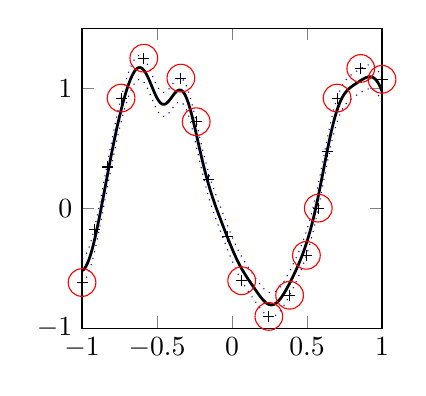
\begin{tikzpicture}

\begin{axis}[%
width=1.5in,
height=1.5in,
scale only axis,
xmin=-1,
xmax=1,
ymin=-1,
ymax=1.5,
]
\addplot [color=black,solid,line width=1.0pt,forget plot]
  table[row sep=crcr]{%
-1	-0.519478094668077\\
-0.993333333333333	-0.514825507574742\\
-0.986666666666667	-0.507262094265251\\
-0.98	-0.496773788492693\\
-0.973333333333333	-0.483374036442919\\
-0.966666666666667	-0.467102700679731\\
-0.96	-0.44802449180788\\
-0.953333333333333	-0.426226996583418\\
-0.946666666666667	-0.401818381592594\\
-0.94	-0.374924858241789\\
-0.933333333333333	-0.345687997429841\\
-0.926666666666667	-0.314261980903266\\
-0.92	-0.280810871133675\\
-0.913333333333333	-0.245505973018918\\
-0.906666666666667	-0.208523349390497\\
-0.9	-0.170041538950641\\
-0.893333333333333	-0.130239510707106\\
-0.886666666666667	-0.0892948741173161\\
-0.88	-0.0473823498889232\\
-0.873333333333333	-0.0046724935464809\\
-0.866666666666667	0.0386693468097557\\
-0.86	0.0824838650853762\\
-0.853333333333333	0.12661845549901\\
-0.846666666666667	0.170927727583658\\
-0.84	0.215273909227987\\
-0.833333333333333	0.259527164564083\\
-0.826666666666667	0.303565846549517\\
-0.82	0.347276695387817\\
-0.813333333333333	0.390554984291195\\
-0.806666666666667	0.433304604402104\\
-0.8	0.475438071866985\\
-0.793333333333333	0.516876432966788\\
-0.786666666666667	0.557549038621734\\
-0.78	0.597393158110438\\
-0.773333333333333	0.636353403876038\\
-0.766666666666667	0.674380944990661\\
-0.76	0.711432496105813\\
-0.753333333333333	0.747469081151547\\
-0.746666666666667	0.782454586026612\\
-0.74	0.816354131184007\\
-0.733333333333333	0.849132312320434\\
-0.726666666666667	0.88075137416338\\
-0.72	0.911169397405715\\
-0.713333333333333	0.94033859098118\\
-0.706666666666667	0.968203790025453\\
-0.7	0.994701263125414\\
-0.693333333333333	1.01975793016568\\
-0.686666666666667	1.04329108387454\\
-0.68	1.06520869402101\\
-0.673333333333333	1.08541035343889\\
-0.666666666666667	1.10378890031529\\
-0.66	1.12023272246109\\
-0.653333333333333	1.13462871783435\\
-0.646666666666667	1.14686585288109\\
-0.64	1.15683922789175\\
-0.633333333333333	1.16445452819591\\
-0.626666666666667	1.16963271324102\\
-0.62	1.17231477390253\\
-0.613333333333333	1.17246637301973\\
-0.606666666666667	1.17008217612957\\
-0.6	1.16518967932675\\
-0.593333333333333	1.15785234938695\\
-0.586666666666667	1.14817190763488\\
-0.58	1.13628961302065\\
-0.573333333333333	1.12238643062681\\
-0.566666666666667	1.10668200819173\\
-0.56	1.08943242377215\\
-0.553333333333333	1.07092671076492\\
-0.546666666666667	1.0514822104433\\
-0.54	1.03143884518773\\
-0.533333333333333	1.0111524460085\\
-0.526666666666667	0.990987304195452\\
-0.52	0.971308147603792\\
-0.513333333333333	0.952471766050984\\
-0.506666666666667	0.934818526691282\\
-0.5	0.918664028488233\\
-0.493333333333333	0.904291144770123\\
-0.486666666666667	0.891942694387121\\
-0.48	0.8818149655445\\
-0.473333333333333	0.874052292586399\\
-0.466666666666667	0.868742855708956\\
-0.46	0.865915837849192\\
-0.453333333333333	0.865540033042672\\
-0.446666666666667	0.867523957697591\\
-0.44	0.871717471892851\\
-0.433333333333333	0.877914873394389\\
-0.426666666666667	0.885859384000753\\
-0.42	0.895248907419515\\
-0.413333333333333	0.905742901386963\\
-0.406666666666667	0.916970175288169\\
-0.4	0.928537399061029\\
-0.393333333333333	0.940038090431452\\
-0.386666666666667	0.951061836065378\\
-0.38	0.961203498339904\\
-0.373333333333333	0.970072163186622\\
-0.366666666666667	0.977299595650559\\
-0.36	0.982547987995267\\
-0.353333333333333	0.985516809691437\\
-0.346666666666667	0.985948598561891\\
-0.34	0.983633566646007\\
-0.333333333333333	0.978412931772933\\
-0.326666666666667	0.97018092507787\\
-0.32	0.958885464393412\\
-0.313333333333333	0.944527522238603\\
-0.306666666666667	0.927159253712247\\
-0.3	0.906880982787093\\
-0.293333333333333	0.883837174270839\\
-0.286666666666667	0.858211542221693\\
-0.28	0.830221463284399\\
-0.273333333333333	0.800111874900607\\
-0.266666666666667	0.76814884355565\\
-0.26	0.734612987312948\\
-0.253333333333333	0.699792930251523\\
-0.246666666666667	0.663978954659455\\
-0.24	0.627457000710937\\
-0.233333333333333	0.590503143752884\\
-0.226666666666667	0.553378657208214\\
-0.22	0.516325745449658\\
-0.213333333333333	0.479564006769197\\
-0.206666666666667	0.443287662655236\\
-0.2	0.407663566779669\\
-0.193333333333333	0.372829986045469\\
-0.186666666666667	0.338896127256662\\
-0.18	0.30594236679228\\
-0.173333333333333	0.274021127281851\\
-0.166666666666667	0.243158334733012\\
-0.16	0.213355381763914\\
-0.153333333333333	0.184591517351692\\
-0.146666666666667	0.156826580554573\\
-0.14	0.130003994684364\\
-0.133333333333333	0.104053939066646\\
-0.126666666666667	0.0788966175079007\\
-0.12	0.0544455456059252\\
-0.113333333333333	0.0306107828586425\\
-0.106666666666667	0.00730203997693778\\
-0.1	-0.0155684032123372\\
-0.0933333333333333	-0.0380830284118963\\
-0.0866666666666666	-0.0603167111951857\\
-0.08	-0.0823347016170069\\
-0.0733333333333333	-0.104190992422378\\
-0.0666666666666667	-0.125927106171843\\
-0.0599999999999999	-0.147571323750008\\
-0.0533333333333332	-0.169138366996416\\
-0.0466666666666666	-0.190629537617701\\
-0.0399999999999999	-0.212033303205099\\
-0.0333333333333333	-0.233326309273542\\
-0.0266666666666666	-0.254474784026777\\
-0.0199999999999999	-0.275436290389981\\
-0.0133333333333333	-0.296161768163145\\
-0.0066666666666666	-0.316597798416668\\
1.11022302462516e-16	-0.336689012988835\\
0.00666666666666682	-0.356380564670765\\
0.0133333333333335	-0.37562056886769\\
0.0200000000000001	-0.394362425634874\\
0.0266666666666668	-0.412566932337916\\
0.0333333333333335	-0.43020410199355\\
0.0400000000000001	-0.447254610674344\\
0.0466666666666669	-0.463710809109887\\
0.0533333333333335	-0.479577248515177\\
0.0600000000000002	-0.494870688277101\\
0.0666666666666669	-0.50961957282215\\
0.0733333333333335	-0.523862986020261\\
0.0800000000000002	-0.537649112986104\\
0.0866666666666668	-0.551033260181912\\
0.0933333333333335	-0.564075504338108\\
0.1	-0.57683805794353\\
0.106666666666667	-0.589382453041292\\
0.113333333333334	-0.601766655045772\\
0.12	-0.614042223682689\\
0.126666666666667	-0.626251638563514\\
0.133333333333334	-0.63842590218416\\
0.14	-0.650582523380542\\
0.146666666666667	-0.662723969824937\\
0.153333333333334	-0.674836659591712\\
0.16	-0.686890539958641\\
0.166666666666667	-0.698839277418844\\
0.173333333333333	-0.710621057466641\\
0.18	-0.722159967270987\\
0.186666666666667	-0.733367910058109\\
0.193333333333333	-0.744146978035601\\
0.2	-0.754392192037305\\
0.206666666666667	-0.763994501618336\\
0.213333333333333	-0.772843929735327\\
0.22	-0.780832741812112\\
0.226666666666667	-0.787858520049519\\
0.233333333333334	-0.793827030147799\\
0.24	-0.79865477876357\\
0.246666666666667	-0.802271175371397\\
0.253333333333334	-0.804620230892196\\
0.26	-0.805661746483169\\
0.266666666666667	-0.805371968159174\\
0.273333333333334	-0.803743705303894\\
0.28	-0.800785932533307\\
0.286666666666667	-0.796522913788245\\
0.293333333333334	-0.790992904097646\\
0.3	-0.784246497499239\\
0.306666666666667	-0.776344698680521\\
0.313333333333333	-0.767356800798843\\
0.32	-0.757358152684601\\
0.326666666666667	-0.746427895484158\\
0.333333333333333	-0.73464674222067\\
0.34	-0.722094864369505\\
0.346666666666667	-0.708849938110029\\
0.353333333333333	-0.694985390246883\\
0.36	-0.680568870728866\\
0.366666666666667	-0.665660966035102\\
0.373333333333334	-0.650314156167704\\
0.38	-0.634572008187398\\
0.386666666666667	-0.618468591601073\\
0.393333333333334	-0.602028095733454\\
0.4	-0.585264626584119\\
0.406666666666667	-0.568182160504194\\
0.413333333333334	-0.550774634079151\\
0.42	-0.533026153490408\\
0.426666666666667	-0.514911311854692\\
0.433333333333334	-0.496395609038609\\
0.44	-0.477435974613652\\
0.446666666666667	-0.457981400354884\\
0.453333333333333	-0.437973693436389\\
0.46	-0.41734836475391\\
0.466666666666667	-0.396035668227456\\
0.473333333333333	-0.373961806244625\\
0.48	-0.351050313476832\\
0.486666666666667	-0.327223626156935\\
0.493333333333334	-0.302404836711895\\
0.5	-0.276519624696457\\
0.506666666666667	-0.249498344691474\\
0.513333333333334	-0.221278240731125\\
0.52	-0.191805745499527\\
0.526666666666667	-0.161038811628112\\
0.533333333333334	-0.128949212585845\\
0.54	-0.0955247425240781\\
0.546666666666667	-0.0607712386079747\\
0.553333333333333	-0.0247143463500237\\
0.56	0.0125990513358689\\
0.566666666666667	0.0510998169448625\\
0.573333333333333	0.0906960213297685\\
0.58	0.131272944179338\\
0.586666666666667	0.172693655185291\\
0.593333333333333	0.214800201868154\\
0.6	0.257415410447664\\
0.606666666666667	0.300345284875012\\
0.613333333333334	0.34338196702762\\
0.62	0.386307199030501\\
0.626666666666667	0.428896207691445\\
0.633333333333334	0.470921912106654\\
0.64	0.512159339552569\\
0.646666666666667	0.552390122679563\\
0.653333333333334	0.591406943473821\\
0.66	0.629017786979937\\
0.666666666666667	0.665049870681707\\
0.673333333333334	0.69935312377759\\
0.68	0.731803104152811\\
0.686666666666667	0.762303259172008\\
0.693333333333334	0.790786458776182\\
0.7	0.817215754827647\\
0.706666666666667	0.841584348092912\\
0.713333333333334	0.863914772450805\\
0.72	0.884257333569713\\
0.726666666666667	0.902687865133765\\
0.733333333333334	0.919304888517337\\
0.74	0.934226280566196\\
0.746666666666667	0.947585568010347\\
0.753333333333334	0.959527975438559\\
0.76	0.970206356434441\\
0.766666666666667	0.979777134448876\\
0.773333333333334	0.988396371614879\\
0.78	0.996216070639469\\
0.786666666666667	1.00338079802393\\
0.793333333333334	1.01002469725387\\
0.8	1.01626893947473\\
0.806666666666667	1.02221963778673\\
0.813333333333334	1.02796623088548\\
0.82	1.03358032346127\\
0.826666666666667	1.03911495549464\\
0.833333333333333	1.04460426105335\\
0.84	1.05006346983408\\
0.846666666666667	1.05548920162571\\
0.853333333333333	1.06086000492194\\
0.86	1.0661370956154\\
0.866666666666667	1.07126525935204\\
0.873333333333334	1.07617389081144\\
0.88	1.08077815387846\\
0.886666666666667	1.08498025731003\\
0.893333333333334	1.08867085003511\\
0.9	1.09173054771923\\
0.906666666666667	1.09403160691782\\
0.913333333333334	1.09543976450411\\
0.92	1.09581625782508\\
0.926666666666667	1.09502003523908\\
0.933333333333334	1.09291015763019\\
0.94	1.08934837975161\\
0.946666666666667	1.08420188661785\\
0.953333333333334	1.07734614560593\\
0.96	1.0686678204974\\
0.966666666666667	1.05806768048134\\
0.973333333333334	1.04546342617451\\
0.98	1.03079234690829\\
0.986666666666667	1.01401371960773\\
0.993333333333334	0.995110860033359\\
1	0.974092742194648\\
};
\addplot [color=blue,dotted,forget plot]
  table[row sep=crcr]{%
-1	-0.419478094668077\\
-0.993333333333333	-0.414825507574742\\
-0.986666666666667	-0.407262094265251\\
-0.98	-0.396773788492693\\
-0.973333333333333	-0.383374036442919\\
-0.966666666666667	-0.367102700679731\\
-0.96	-0.34802449180788\\
-0.953333333333333	-0.326226996583418\\
-0.946666666666667	-0.301818381592594\\
-0.94	-0.274924858241789\\
-0.933333333333333	-0.245687997429841\\
-0.926666666666667	-0.214261980903266\\
-0.92	-0.180810871133675\\
-0.913333333333333	-0.145505973018918\\
-0.906666666666667	-0.108523349390497\\
-0.9	-0.0700415389506414\\
-0.893333333333333	-0.0302395107071056\\
-0.886666666666667	0.0107051258826839\\
-0.88	0.0526176501110768\\
-0.873333333333333	0.0953275064535191\\
-0.866666666666667	0.138669346809756\\
-0.86	0.182483865085376\\
-0.853333333333333	0.22661845549901\\
-0.846666666666667	0.270927727583658\\
-0.84	0.315273909227987\\
-0.833333333333333	0.359527164564083\\
-0.826666666666667	0.403565846549517\\
-0.82	0.447276695387817\\
-0.813333333333333	0.490554984291195\\
-0.806666666666667	0.533304604402104\\
-0.8	0.575438071866985\\
-0.793333333333333	0.616876432966788\\
-0.786666666666667	0.657549038621734\\
-0.78	0.697393158110438\\
-0.773333333333333	0.736353403876038\\
-0.766666666666667	0.774380944990661\\
-0.76	0.811432496105813\\
-0.753333333333333	0.847469081151547\\
-0.746666666666667	0.882454586026612\\
-0.74	0.916354131184007\\
-0.733333333333333	0.949132312320434\\
-0.726666666666667	0.98075137416338\\
-0.72	1.01116939740571\\
-0.713333333333333	1.04033859098118\\
-0.706666666666667	1.06820379002545\\
-0.7	1.09470126312541\\
-0.693333333333333	1.11975793016568\\
-0.686666666666667	1.14329108387454\\
-0.68	1.16520869402101\\
-0.673333333333333	1.18541035343889\\
-0.666666666666667	1.20378890031529\\
-0.66	1.22023272246109\\
-0.653333333333333	1.23462871783435\\
-0.646666666666667	1.24686585288109\\
-0.64	1.25683922789175\\
-0.633333333333333	1.26445452819591\\
-0.626666666666667	1.26963271324102\\
-0.62	1.27231477390253\\
-0.613333333333333	1.27246637301973\\
-0.606666666666667	1.27008217612957\\
-0.6	1.26518967932675\\
-0.593333333333333	1.25785234938695\\
-0.586666666666667	1.24817190763488\\
-0.58	1.23628961302065\\
-0.573333333333333	1.22238643062681\\
-0.566666666666667	1.20668200819173\\
-0.56	1.18943242377215\\
-0.553333333333333	1.17092671076492\\
-0.546666666666667	1.1514822104433\\
-0.54	1.13143884518773\\
-0.533333333333333	1.1111524460085\\
-0.526666666666667	1.09098730419545\\
-0.52	1.07130814760379\\
-0.513333333333333	1.05247176605098\\
-0.506666666666667	1.03481852669128\\
-0.5	1.01866402848823\\
-0.493333333333333	1.00429114477012\\
-0.486666666666667	0.991942694387121\\
-0.48	0.9818149655445\\
-0.473333333333333	0.974052292586399\\
-0.466666666666667	0.968742855708956\\
-0.46	0.965915837849192\\
-0.453333333333333	0.965540033042672\\
-0.446666666666667	0.967523957697591\\
-0.44	0.971717471892851\\
-0.433333333333333	0.977914873394389\\
-0.426666666666667	0.985859384000753\\
-0.42	0.995248907419515\\
-0.413333333333333	1.00574290138696\\
-0.406666666666667	1.01697017528817\\
-0.4	1.02853739906103\\
-0.393333333333333	1.04003809043145\\
-0.386666666666667	1.05106183606538\\
-0.38	1.0612034983399\\
-0.373333333333333	1.07007216318662\\
-0.366666666666667	1.07729959565056\\
-0.36	1.08254798799527\\
-0.353333333333333	1.08551680969144\\
-0.346666666666667	1.08594859856189\\
-0.34	1.08363356664601\\
-0.333333333333333	1.07841293177293\\
-0.326666666666667	1.07018092507787\\
-0.32	1.05888546439341\\
-0.313333333333333	1.0445275222386\\
-0.306666666666667	1.02715925371225\\
-0.3	1.00688098278709\\
-0.293333333333333	0.983837174270839\\
-0.286666666666667	0.958211542221693\\
-0.28	0.930221463284399\\
-0.273333333333333	0.900111874900607\\
-0.266666666666667	0.86814884355565\\
-0.26	0.834612987312948\\
-0.253333333333333	0.799792930251523\\
-0.246666666666667	0.763978954659455\\
-0.24	0.727457000710937\\
-0.233333333333333	0.690503143752884\\
-0.226666666666667	0.653378657208214\\
-0.22	0.616325745449658\\
-0.213333333333333	0.579564006769197\\
-0.206666666666667	0.543287662655236\\
-0.2	0.507663566779669\\
-0.193333333333333	0.472829986045469\\
-0.186666666666667	0.438896127256662\\
-0.18	0.40594236679228\\
-0.173333333333333	0.374021127281851\\
-0.166666666666667	0.343158334733012\\
-0.16	0.313355381763914\\
-0.153333333333333	0.284591517351692\\
-0.146666666666667	0.256826580554573\\
-0.14	0.230003994684364\\
-0.133333333333333	0.204053939066646\\
-0.126666666666667	0.178896617507901\\
-0.12	0.154445545605925\\
-0.113333333333333	0.130610782858643\\
-0.106666666666667	0.107302039976938\\
-0.1	0.0844315967876628\\
-0.0933333333333333	0.0619169715881037\\
-0.0866666666666666	0.0396832888048143\\
-0.08	0.0176652983829931\\
-0.0733333333333333	-0.00419099242237794\\
-0.0666666666666667	-0.0259271061718427\\
-0.0599999999999999	-0.0475713237500079\\
-0.0533333333333332	-0.0691383669964158\\
-0.0466666666666666	-0.0906295376177006\\
-0.0399999999999999	-0.112033303205099\\
-0.0333333333333333	-0.133326309273542\\
-0.0266666666666666	-0.154474784026777\\
-0.0199999999999999	-0.175436290389981\\
-0.0133333333333333	-0.196161768163145\\
-0.0066666666666666	-0.216597798416668\\
1.11022302462516e-16	-0.236689012988835\\
0.00666666666666682	-0.256380564670765\\
0.0133333333333335	-0.27562056886769\\
0.0200000000000001	-0.294362425634874\\
0.0266666666666668	-0.312566932337916\\
0.0333333333333335	-0.33020410199355\\
0.0400000000000001	-0.347254610674344\\
0.0466666666666669	-0.363710809109887\\
0.0533333333333335	-0.379577248515177\\
0.0600000000000002	-0.394870688277101\\
0.0666666666666669	-0.40961957282215\\
0.0733333333333335	-0.423862986020261\\
0.0800000000000002	-0.437649112986104\\
0.0866666666666668	-0.451033260181912\\
0.0933333333333335	-0.464075504338108\\
0.1	-0.47683805794353\\
0.106666666666667	-0.489382453041292\\
0.113333333333334	-0.501766655045772\\
0.12	-0.514042223682689\\
0.126666666666667	-0.526251638563514\\
0.133333333333334	-0.53842590218416\\
0.14	-0.550582523380542\\
0.146666666666667	-0.562723969824937\\
0.153333333333334	-0.574836659591712\\
0.16	-0.586890539958641\\
0.166666666666667	-0.598839277418844\\
0.173333333333333	-0.610621057466641\\
0.18	-0.622159967270987\\
0.186666666666667	-0.633367910058109\\
0.193333333333333	-0.644146978035601\\
0.2	-0.654392192037305\\
0.206666666666667	-0.663994501618336\\
0.213333333333333	-0.672843929735327\\
0.22	-0.680832741812112\\
0.226666666666667	-0.687858520049519\\
0.233333333333334	-0.693827030147799\\
0.24	-0.69865477876357\\
0.246666666666667	-0.702271175371397\\
0.253333333333334	-0.704620230892196\\
0.26	-0.705661746483169\\
0.266666666666667	-0.705371968159174\\
0.273333333333334	-0.703743705303894\\
0.28	-0.700785932533307\\
0.286666666666667	-0.696522913788245\\
0.293333333333334	-0.690992904097646\\
0.3	-0.684246497499239\\
0.306666666666667	-0.676344698680521\\
0.313333333333333	-0.667356800798844\\
0.32	-0.657358152684601\\
0.326666666666667	-0.646427895484158\\
0.333333333333333	-0.63464674222067\\
0.34	-0.622094864369505\\
0.346666666666667	-0.608849938110029\\
0.353333333333333	-0.594985390246883\\
0.36	-0.580568870728866\\
0.366666666666667	-0.565660966035102\\
0.373333333333334	-0.550314156167704\\
0.38	-0.534572008187398\\
0.386666666666667	-0.518468591601073\\
0.393333333333334	-0.502028095733454\\
0.4	-0.485264626584119\\
0.406666666666667	-0.468182160504194\\
0.413333333333334	-0.450774634079151\\
0.42	-0.433026153490408\\
0.426666666666667	-0.414911311854692\\
0.433333333333334	-0.396395609038609\\
0.44	-0.377435974613652\\
0.446666666666667	-0.357981400354884\\
0.453333333333333	-0.337973693436389\\
0.46	-0.31734836475391\\
0.466666666666667	-0.296035668227456\\
0.473333333333333	-0.273961806244625\\
0.48	-0.251050313476832\\
0.486666666666667	-0.227223626156935\\
0.493333333333334	-0.202404836711895\\
0.5	-0.176519624696457\\
0.506666666666667	-0.149498344691474\\
0.513333333333334	-0.121278240731125\\
0.52	-0.0918057454995274\\
0.526666666666667	-0.0610388116281118\\
0.533333333333334	-0.0289492125858445\\
0.54	0.00447525747592188\\
0.546666666666667	0.0392287613920253\\
0.553333333333333	0.0752856536499763\\
0.56	0.112599051335869\\
0.566666666666667	0.151099816944862\\
0.573333333333333	0.190696021329769\\
0.58	0.231272944179338\\
0.586666666666667	0.272693655185291\\
0.593333333333333	0.314800201868154\\
0.6	0.357415410447664\\
0.606666666666667	0.400345284875012\\
0.613333333333334	0.44338196702762\\
0.62	0.486307199030501\\
0.626666666666667	0.528896207691445\\
0.633333333333334	0.570921912106654\\
0.64	0.612159339552569\\
0.646666666666667	0.652390122679563\\
0.653333333333334	0.691406943473821\\
0.66	0.729017786979937\\
0.666666666666667	0.765049870681707\\
0.673333333333334	0.79935312377759\\
0.68	0.831803104152811\\
0.686666666666667	0.862303259172008\\
0.693333333333334	0.890786458776182\\
0.7	0.917215754827647\\
0.706666666666667	0.941584348092912\\
0.713333333333334	0.963914772450805\\
0.72	0.984257333569713\\
0.726666666666667	1.00268786513377\\
0.733333333333334	1.01930488851734\\
0.74	1.0342262805662\\
0.746666666666667	1.04758556801035\\
0.753333333333334	1.05952797543856\\
0.76	1.07020635643444\\
0.766666666666667	1.07977713444888\\
0.773333333333334	1.08839637161488\\
0.78	1.09621607063947\\
0.786666666666667	1.10338079802393\\
0.793333333333334	1.11002469725387\\
0.8	1.11626893947473\\
0.806666666666667	1.12221963778673\\
0.813333333333334	1.12796623088548\\
0.82	1.13358032346127\\
0.826666666666667	1.13911495549464\\
0.833333333333333	1.14460426105335\\
0.84	1.15006346983408\\
0.846666666666667	1.15548920162571\\
0.853333333333333	1.16086000492194\\
0.86	1.1661370956154\\
0.866666666666667	1.17126525935204\\
0.873333333333334	1.17617389081144\\
0.88	1.18077815387846\\
0.886666666666667	1.18498025731003\\
0.893333333333334	1.18867085003511\\
0.9	1.19173054771923\\
0.906666666666667	1.19403160691782\\
0.913333333333334	1.19543976450411\\
0.92	1.19581625782508\\
0.926666666666667	1.19502003523908\\
0.933333333333334	1.19291015763019\\
0.94	1.18934837975161\\
0.946666666666667	1.18420188661785\\
0.953333333333334	1.17734614560593\\
0.96	1.1686678204974\\
0.966666666666667	1.15806768048134\\
0.973333333333334	1.14546342617451\\
0.98	1.13079234690829\\
0.986666666666667	1.11401371960773\\
0.993333333333334	1.09511086003336\\
1	1.07409274219465\\
};
\addplot [color=blue,dotted,forget plot]
  table[row sep=crcr]{%
-1	-0.619478094668077\\
-0.993333333333333	-0.614825507574742\\
-0.986666666666667	-0.607262094265251\\
-0.98	-0.596773788492693\\
-0.973333333333333	-0.583374036442919\\
-0.966666666666667	-0.567102700679731\\
-0.96	-0.54802449180788\\
-0.953333333333333	-0.526226996583418\\
-0.946666666666667	-0.501818381592594\\
-0.94	-0.474924858241789\\
-0.933333333333333	-0.445687997429841\\
-0.926666666666667	-0.414261980903266\\
-0.92	-0.380810871133675\\
-0.913333333333333	-0.345505973018918\\
-0.906666666666667	-0.308523349390497\\
-0.9	-0.270041538950641\\
-0.893333333333333	-0.230239510707106\\
-0.886666666666667	-0.189294874117316\\
-0.88	-0.147382349888923\\
-0.873333333333333	-0.104672493546481\\
-0.866666666666667	-0.0613306531902443\\
-0.86	-0.0175161349146238\\
-0.853333333333333	0.0266184554990097\\
-0.846666666666667	0.0709277275836581\\
-0.84	0.115273909227987\\
-0.833333333333333	0.159527164564083\\
-0.826666666666667	0.203565846549517\\
-0.82	0.247276695387817\\
-0.813333333333333	0.290554984291195\\
-0.806666666666667	0.333304604402104\\
-0.8	0.375438071866985\\
-0.793333333333333	0.416876432966788\\
-0.786666666666667	0.457549038621734\\
-0.78	0.497393158110438\\
-0.773333333333333	0.536353403876038\\
-0.766666666666667	0.574380944990661\\
-0.76	0.611432496105813\\
-0.753333333333333	0.647469081151547\\
-0.746666666666667	0.682454586026612\\
-0.74	0.716354131184007\\
-0.733333333333333	0.749132312320434\\
-0.726666666666667	0.78075137416338\\
-0.72	0.811169397405715\\
-0.713333333333333	0.84033859098118\\
-0.706666666666667	0.868203790025453\\
-0.7	0.894701263125414\\
-0.693333333333333	0.919757930165678\\
-0.686666666666667	0.943291083874541\\
-0.68	0.965208694021012\\
-0.673333333333333	0.985410353438887\\
-0.666666666666667	1.00378890031529\\
-0.66	1.02023272246109\\
-0.653333333333333	1.03462871783435\\
-0.646666666666667	1.04686585288109\\
-0.64	1.05683922789175\\
-0.633333333333333	1.06445452819591\\
-0.626666666666667	1.06963271324102\\
-0.62	1.07231477390253\\
-0.613333333333333	1.07246637301973\\
-0.606666666666667	1.07008217612957\\
-0.6	1.06518967932675\\
-0.593333333333333	1.05785234938695\\
-0.586666666666667	1.04817190763488\\
-0.58	1.03628961302065\\
-0.573333333333333	1.02238643062681\\
-0.566666666666667	1.00668200819173\\
-0.56	0.98943242377215\\
-0.553333333333333	0.970926710764923\\
-0.546666666666667	0.951482210443305\\
-0.54	0.931438845187733\\
-0.533333333333333	0.911152446008501\\
-0.526666666666667	0.890987304195452\\
-0.52	0.871308147603792\\
-0.513333333333333	0.852471766050984\\
-0.506666666666667	0.834818526691282\\
-0.5	0.818664028488233\\
-0.493333333333333	0.804291144770123\\
-0.486666666666667	0.791942694387121\\
-0.48	0.7818149655445\\
-0.473333333333333	0.774052292586399\\
-0.466666666666667	0.768742855708956\\
-0.46	0.765915837849192\\
-0.453333333333333	0.765540033042672\\
-0.446666666666667	0.767523957697591\\
-0.44	0.771717471892851\\
-0.433333333333333	0.777914873394389\\
-0.426666666666667	0.785859384000754\\
-0.42	0.795248907419515\\
-0.413333333333333	0.805742901386963\\
-0.406666666666667	0.816970175288169\\
-0.4	0.828537399061029\\
-0.393333333333333	0.840038090431452\\
-0.386666666666667	0.851061836065378\\
-0.38	0.861203498339904\\
-0.373333333333333	0.870072163186622\\
-0.366666666666667	0.877299595650559\\
-0.36	0.882547987995267\\
-0.353333333333333	0.885516809691437\\
-0.346666666666667	0.885948598561891\\
-0.34	0.883633566646007\\
-0.333333333333333	0.878412931772933\\
-0.326666666666667	0.87018092507787\\
-0.32	0.858885464393412\\
-0.313333333333333	0.844527522238603\\
-0.306666666666667	0.827159253712247\\
-0.3	0.806880982787093\\
-0.293333333333333	0.783837174270839\\
-0.286666666666667	0.758211542221693\\
-0.28	0.730221463284399\\
-0.273333333333333	0.700111874900607\\
-0.266666666666667	0.66814884355565\\
-0.26	0.634612987312948\\
-0.253333333333333	0.599792930251523\\
-0.246666666666667	0.563978954659455\\
-0.24	0.527457000710937\\
-0.233333333333333	0.490503143752884\\
-0.226666666666667	0.453378657208214\\
-0.22	0.416325745449658\\
-0.213333333333333	0.379564006769197\\
-0.206666666666667	0.343287662655236\\
-0.2	0.307663566779669\\
-0.193333333333333	0.272829986045469\\
-0.186666666666667	0.238896127256662\\
-0.18	0.20594236679228\\
-0.173333333333333	0.174021127281851\\
-0.166666666666667	0.143158334733012\\
-0.16	0.113355381763914\\
-0.153333333333333	0.0845915173516917\\
-0.146666666666667	0.0568265805545735\\
-0.14	0.0300039946843644\\
-0.133333333333333	0.00405393906664567\\
-0.126666666666667	-0.0211033824920993\\
-0.12	-0.0455544543940748\\
-0.113333333333333	-0.0693892171413575\\
-0.106666666666667	-0.0926979600230622\\
-0.1	-0.115568403212337\\
-0.0933333333333333	-0.138083028411896\\
-0.0866666666666666	-0.160316711195186\\
-0.08	-0.182334701617007\\
-0.0733333333333333	-0.204190992422378\\
-0.0666666666666667	-0.225927106171843\\
-0.0599999999999999	-0.247571323750008\\
-0.0533333333333332	-0.269138366996416\\
-0.0466666666666666	-0.290629537617701\\
-0.0399999999999999	-0.312033303205099\\
-0.0333333333333333	-0.333326309273542\\
-0.0266666666666666	-0.354474784026777\\
-0.0199999999999999	-0.375436290389981\\
-0.0133333333333333	-0.396161768163145\\
-0.0066666666666666	-0.416597798416668\\
1.11022302462516e-16	-0.436689012988835\\
0.00666666666666682	-0.456380564670765\\
0.0133333333333335	-0.47562056886769\\
0.0200000000000001	-0.494362425634874\\
0.0266666666666668	-0.512566932337916\\
0.0333333333333335	-0.530204101993551\\
0.0400000000000001	-0.547254610674344\\
0.0466666666666669	-0.563710809109887\\
0.0533333333333335	-0.579577248515177\\
0.0600000000000002	-0.594870688277101\\
0.0666666666666669	-0.60961957282215\\
0.0733333333333335	-0.623862986020261\\
0.0800000000000002	-0.637649112986104\\
0.0866666666666668	-0.651033260181912\\
0.0933333333333335	-0.664075504338108\\
0.1	-0.67683805794353\\
0.106666666666667	-0.689382453041292\\
0.113333333333334	-0.701766655045772\\
0.12	-0.714042223682689\\
0.126666666666667	-0.726251638563514\\
0.133333333333334	-0.73842590218416\\
0.14	-0.750582523380542\\
0.146666666666667	-0.762723969824937\\
0.153333333333334	-0.774836659591712\\
0.16	-0.786890539958641\\
0.166666666666667	-0.798839277418844\\
0.173333333333333	-0.810621057466641\\
0.18	-0.822159967270987\\
0.186666666666667	-0.833367910058109\\
0.193333333333333	-0.844146978035601\\
0.2	-0.854392192037305\\
0.206666666666667	-0.863994501618336\\
0.213333333333333	-0.872843929735327\\
0.22	-0.880832741812112\\
0.226666666666667	-0.887858520049518\\
0.233333333333334	-0.893827030147799\\
0.24	-0.89865477876357\\
0.246666666666667	-0.902271175371397\\
0.253333333333334	-0.904620230892196\\
0.26	-0.905661746483169\\
0.266666666666667	-0.905371968159174\\
0.273333333333334	-0.903743705303894\\
0.28	-0.900785932533307\\
0.286666666666667	-0.896522913788245\\
0.293333333333334	-0.890992904097646\\
0.3	-0.884246497499239\\
0.306666666666667	-0.876344698680521\\
0.313333333333333	-0.867356800798843\\
0.32	-0.857358152684601\\
0.326666666666667	-0.846427895484158\\
0.333333333333333	-0.83464674222067\\
0.34	-0.822094864369505\\
0.346666666666667	-0.808849938110029\\
0.353333333333333	-0.794985390246883\\
0.36	-0.780568870728866\\
0.366666666666667	-0.765660966035102\\
0.373333333333334	-0.750314156167704\\
0.38	-0.734572008187398\\
0.386666666666667	-0.718468591601073\\
0.393333333333334	-0.702028095733454\\
0.4	-0.685264626584119\\
0.406666666666667	-0.668182160504194\\
0.413333333333334	-0.650774634079151\\
0.42	-0.633026153490408\\
0.426666666666667	-0.614911311854692\\
0.433333333333334	-0.596395609038609\\
0.44	-0.577435974613652\\
0.446666666666667	-0.557981400354884\\
0.453333333333333	-0.537973693436389\\
0.46	-0.51734836475391\\
0.466666666666667	-0.496035668227456\\
0.473333333333333	-0.473961806244625\\
0.48	-0.451050313476832\\
0.486666666666667	-0.427223626156935\\
0.493333333333334	-0.402404836711895\\
0.5	-0.376519624696457\\
0.506666666666667	-0.349498344691474\\
0.513333333333334	-0.321278240731125\\
0.52	-0.291805745499527\\
0.526666666666667	-0.261038811628112\\
0.533333333333334	-0.228949212585845\\
0.54	-0.195524742524078\\
0.546666666666667	-0.160771238607975\\
0.553333333333333	-0.124714346350024\\
0.56	-0.0874009486641311\\
0.566666666666667	-0.0489001830551375\\
0.573333333333333	-0.0093039786702315\\
0.58	0.0312729441793378\\
0.586666666666667	0.0726936551852912\\
0.593333333333333	0.114800201868154\\
0.6	0.157415410447664\\
0.606666666666667	0.200345284875012\\
0.613333333333334	0.24338196702762\\
0.62	0.286307199030501\\
0.626666666666667	0.328896207691445\\
0.633333333333334	0.370921912106654\\
0.64	0.412159339552569\\
0.646666666666667	0.452390122679563\\
0.653333333333334	0.491406943473821\\
0.66	0.529017786979937\\
0.666666666666667	0.565049870681707\\
0.673333333333334	0.59935312377759\\
0.68	0.631803104152811\\
0.686666666666667	0.662303259172008\\
0.693333333333334	0.690786458776182\\
0.7	0.717215754827647\\
0.706666666666667	0.741584348092912\\
0.713333333333334	0.763914772450805\\
0.72	0.784257333569713\\
0.726666666666667	0.802687865133765\\
0.733333333333334	0.819304888517337\\
0.74	0.834226280566196\\
0.746666666666667	0.847585568010347\\
0.753333333333334	0.859527975438559\\
0.76	0.870206356434441\\
0.766666666666667	0.879777134448876\\
0.773333333333334	0.888396371614879\\
0.78	0.89621607063947\\
0.786666666666667	0.90338079802393\\
0.793333333333334	0.910024697253871\\
0.8	0.916268939474728\\
0.806666666666667	0.922219637786728\\
0.813333333333334	0.927966230885479\\
0.82	0.933580323461274\\
0.826666666666667	0.939114955494644\\
0.833333333333333	0.944604261053352\\
0.84	0.950063469834083\\
0.846666666666667	0.955489201625707\\
0.853333333333333	0.960860004921936\\
0.86	0.966137095615399\\
0.866666666666667	0.971265259352041\\
0.873333333333334	0.976173890811445\\
0.88	0.98077815387846\\
0.886666666666667	0.984980257310029\\
0.893333333333334	0.988670850035113\\
0.9	0.991730547719227\\
0.906666666666667	0.994031606917818\\
0.913333333333334	0.995439764504106\\
0.92	0.99581625782508\\
0.926666666666667	0.99502003523908\\
0.933333333333334	0.992910157630194\\
0.94	0.989348379751606\\
0.946666666666667	0.984201886617849\\
0.953333333333334	0.977346145605931\\
0.96	0.968667820497397\\
0.966666666666667	0.958067680481341\\
0.973333333333334	0.945463426174507\\
0.98	0.930792346908292\\
0.986666666666667	0.914013719607729\\
0.993333333333334	0.895110860033359\\
1	0.874092742194648\\
};
\addplot [color=black,only marks,mark=+,mark options={solid},forget plot]
  table[row sep=crcr]{%
-1	-0.61945564516129\\
};
\addplot [color=red,mark size=5.0pt,only marks,mark=o,mark options={solid},forget plot]
  table[row sep=crcr]{%
-1	-0.61945564516129\\
};
\addplot [color=black,only marks,mark=+,mark options={solid},forget plot]
  table[row sep=crcr]{%
-0.917627677100494	-0.175907258064516\\
};
\addplot [color=black,only marks,mark=+,mark options={solid},forget plot]
  table[row sep=crcr]{%
-0.828665568369028	0.343245967741936\\
};
\addplot [color=black,only marks,mark=+,mark options={solid},forget plot]
  table[row sep=crcr]{%
-0.739703459637562	0.917842741935484\\
};
\addplot [color=red,mark size=5.0pt,only marks,mark=o,mark options={solid},forget plot]
  table[row sep=crcr]{%
-0.739703459637562	0.917842741935484\\
};
\addplot [color=black,only marks,mark=+,mark options={solid},forget plot]
  table[row sep=crcr]{%
-0.588138385502471	1.25050403225806\\
};
\addplot [color=red,mark size=5.0pt,only marks,mark=o,mark options={solid},forget plot]
  table[row sep=crcr]{%
-0.588138385502471	1.25050403225806\\
};
\addplot [color=black,only marks,mark=+,mark options={solid},forget plot]
  table[row sep=crcr]{%
-0.341021416803954	1.08417338709677\\
};
\addplot [color=red,mark size=5.0pt,only marks,mark=o,mark options={solid},forget plot]
  table[row sep=crcr]{%
-0.341021416803954	1.08417338709677\\
};
\addplot [color=black,only marks,mark=+,mark options={solid},forget plot]
  table[row sep=crcr]{%
-0.238879736408567	0.721270161290323\\
};
\addplot [color=red,mark size=5.0pt,only marks,mark=o,mark options={solid},forget plot]
  table[row sep=crcr]{%
-0.238879736408567	0.721270161290323\\
};
\addplot [color=black,only marks,mark=+,mark options={solid},forget plot]
  table[row sep=crcr]{%
-0.156507413509061	0.237399193548388\\
};
\addplot [color=black,only marks,mark=+,mark options={solid},forget plot]
  table[row sep=crcr]{%
-0.0280065897858319	-0.236391129032258\\
};
\addplot [color=black,only marks,mark=+,mark options={solid},forget plot]
  table[row sep=crcr]{%
0.0642504118616145	-0.604334677419354\\
};
\addplot [color=red,mark size=5.0pt,only marks,mark=o,mark options={solid},forget plot]
  table[row sep=crcr]{%
0.0642504118616145	-0.604334677419354\\
};
\addplot [color=black,only marks,mark=+,mark options={solid},forget plot]
  table[row sep=crcr]{%
0.245469522240527	-0.901713709677419\\
};
\addplot [color=red,mark size=5.0pt,only marks,mark=o,mark options={solid},forget plot]
  table[row sep=crcr]{%
0.245469522240527	-0.901713709677419\\
};
\addplot [color=black,only marks,mark=+,mark options={solid},forget plot]
  table[row sep=crcr]{%
0.383855024711697	-0.725302419354838\\
};
\addplot [color=red,mark size=5.0pt,only marks,mark=o,mark options={solid},forget plot]
  table[row sep=crcr]{%
0.383855024711697	-0.725302419354838\\
};
\addplot [color=black,only marks,mark=+,mark options={solid},forget plot]
  table[row sep=crcr]{%
0.495881383855025	-0.392641129032258\\
};
\addplot [color=red,mark size=5.0pt,only marks,mark=o,mark options={solid},forget plot]
  table[row sep=crcr]{%
0.495881383855025	-0.392641129032258\\
};
\addplot [color=black,only marks,mark=+,mark options={solid},forget plot]
  table[row sep=crcr]{%
0.574958813838551	0.000504032258065168\\
};
\addplot [color=red,mark size=5.0pt,only marks,mark=o,mark options={solid},forget plot]
  table[row sep=crcr]{%
0.574958813838551	0.000504032258065168\\
};
\addplot [color=black,only marks,mark=+,mark options={solid},forget plot]
  table[row sep=crcr]{%
0.634266886326194	0.469254032258065\\
};
\addplot [color=black,only marks,mark=+,mark options={solid},forget plot]
  table[row sep=crcr]{%
0.700164744645799	0.917842741935484\\
};
\addplot [color=red,mark size=5.0pt,only marks,mark=o,mark options={solid},forget plot]
  table[row sep=crcr]{%
0.700164744645799	0.917842741935484\\
};
\addplot [color=black,only marks,mark=+,mark options={solid},forget plot]
  table[row sep=crcr]{%
0.85831960461285	1.1648185483871\\
};
\addplot [color=red,mark size=5.0pt,only marks,mark=o,mark options={solid},forget plot]
  table[row sep=crcr]{%
0.85831960461285	1.1648185483871\\
};
\addplot [color=black,only marks,mark=+,mark options={solid},forget plot]
  table[row sep=crcr]{%
1	1.07409274193548\\
};
\addplot [color=red,mark size=5.0pt,only marks,mark=o,mark options={solid},forget plot]
  table[row sep=crcr]{%
1	1.07409274193548\\
};
\end{axis}
\end{tikzpicture}%
\end{document}
% This file was created by matlab2tikz.
% Minimal pgfplots version: 1.3
%
%The latest updates can be retrieved from
%  http://www.mathworks.com/matlabcentral/fileexchange/22022-matlab2tikz
%where you can also make suggestions and rate matlab2tikz.
%
\documentclass[tikz]{standalone}
\usepackage{pgfplots}
\usepackage{grffile}
\pgfplotsset{compat=newest}
\usetikzlibrary{plotmarks}
\usepackage{amsmath}

\begin{document}
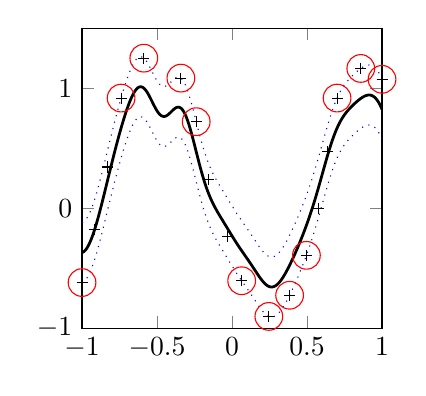
\begin{tikzpicture}

\begin{axis}[%
width=1.5in,
height=1.5in,
scale only axis,
xmin=-1,
xmax=1,
ymin=-1,
ymax=1.5,
]
\addplot [color=black,solid,line width=1.0pt,forget plot]
  table[row sep=crcr]{%
-1	-0.369455646991128\\
-0.993333333333333	-0.365916868887091\\
-0.986666666666667	-0.360266343254397\\
-0.98	-0.352489752410029\\
-0.973333333333333	-0.342592114305454\\
-0.966666666666667	-0.330597015339957\\
-0.96	-0.316545511363422\\
-0.953333333333333	-0.300494745649599\\
-0.946666666666667	-0.282516339807201\\
-0.94	-0.26269461808719\\
-0.933333333333333	-0.241124727195289\\
-0.926666666666667	-0.217910712539615\\
-0.92	-0.193163608000539\\
-0.913333333333333	-0.166999590116738\\
-0.906666666666667	-0.139538239479913\\
-0.9	-0.110900942665605\\
-0.893333333333333	-0.0812094578139336\\
-0.886666666666667	-0.0505846566592942\\
-0.88	-0.0191454460319063\\
-0.873333333333333	0.0129921367913413\\
-0.866666666666667	0.0457156675181953\\
-0.86	0.0789169346711418\\
-0.853333333333333	0.112492416153036\\
-0.846666666666667	0.146343653261192\\
-0.84	0.18037754098664\\
-0.833333333333333	0.214506549564685\\
-0.826666666666667	0.248648886788117\\
-0.82	0.282728604092392\\
-0.813333333333333	0.316675642502783\\
-0.806666666666667	0.350425807878081\\
-0.8	0.383920659179892\\
-0.793333333333333	0.417107289383629\\
-0.786666666666667	0.44993797667844\\
-0.78	0.482369684196\\
-0.773333333333333	0.514363389908993\\
-0.766666666666667	0.545883234599376\\
-0.76	0.576895484752555\\
-0.753333333333333	0.607367318512542\\
-0.746666666666667	0.637265455861439\\
-0.74	0.666554668217902\\
-0.733333333333333	0.695196216803771\\
-0.726666666666667	0.723146282442732\\
-0.72	0.750354460941233\\
-0.713333333333333	0.776762406908424\\
-0.706666666666667	0.80230271394709\\
-0.7	0.826898119899598\\
-0.693333333333333	0.850461121781538\\
-0.686666666666667	0.872894075953906\\
-0.68	0.894089845025592\\
-0.673333333333333	0.913933034286156\\
-0.666666666666667	0.932301837774219\\
-0.66	0.949070488280854\\
-0.653333333333333	0.964112277783129\\
-0.646666666666667	0.977303086280926\\
-0.64	0.988525329152485\\
-0.633333333333333	0.997672207361961\\
-0.626666666666667	1.00465212250947\\
-0.62	1.00939310105274\\
-0.613333333333333	1.01184706010154\\
-0.606666666666667	1.01199374179367\\
-0.6	1.00984414491347\\
-0.593333333333333	1.00544329129455\\
-0.586666666666667	0.998872180507151\\
-0.58	0.990248808887341\\
-0.573333333333333	0.979728157333298\\
-0.566666666666667	0.967501085419764\\
-0.56	0.953792105995657\\
-0.553333333333333	0.938856053107213\\
-0.546666666666667	0.922973695317668\\
-0.54	0.906446384743018\\
-0.533333333333333	0.889589867909146\\
-0.526666666666667	0.872727416486134\\
-0.52	0.856182462863697\\
-0.513333333333333	0.840270946398944\\
-0.506666666666667	0.825293590237865\\
-0.5	0.81152833539144\\
-0.493333333333333	0.799223158014341\\
-0.486666666666667	0.788589487636635\\
-0.48	0.779796428742335\\
-0.473333333333333	0.772965966115978\\
-0.466666666666667	0.768169306543109\\
-0.46	0.765424476685067\\
-0.453333333333333	0.764695260328823\\
-0.446666666666667	0.76589151892175\\
-0.44	0.768870898591188\\
-0.433333333333333	0.773441886002464\\
-0.426666666666667	0.779368135703839\\
-0.42	0.786373954277393\\
-0.413333333333333	0.794150792818768\\
-0.406666666666667	0.80236457005336\\
-0.4	0.810663624668186\\
-0.393333333333333	0.818687077934171\\
-0.386666666666667	0.826073376956041\\
-0.38	0.832468785245476\\
-0.373333333333333	0.837535590868356\\
-0.366666666666667	0.840959813033002\\
-0.36	0.842458205290835\\
-0.353333333333333	0.841784376912744\\
-0.346666666666667	0.838733882670808\\
-0.34	0.833148164197502\\
-0.333333333333333	0.824917262163055\\
-0.326666666666667	0.813981256447309\\
-0.32	0.800330429964389\\
-0.313333333333333	0.784004189496788\\
-0.306666666666667	0.765088812523892\\
-0.3	0.743714121399066\\
-0.293333333333333	0.720049214294634\\
-0.286666666666667	0.694297405238646\\
-0.28	0.666690542675461\\
-0.273333333333333	0.637482886902178\\
-0.266666666666667	0.606944731328784\\
-0.26	0.575355950899215\\
-0.253333333333333	0.542999653552084\\
-0.246666666666667	0.51015609786784\\
-0.24	0.477097022799074\\
-0.233333333333333	0.444080514506777\\
-0.226666666666667	0.411346511813126\\
-0.22	0.379113026657734\\
-0.213333333333333	0.347573130228364\\
-0.206666666666667	0.316892730093856\\
-0.2	0.287209139566922\\
-0.193333333333333	0.258630418410546\\
-0.186666666666667	0.231235444465565\\
-0.18	0.205074659244595\\
-0.173333333333333	0.180171417265326\\
-0.166666666666667	0.156523858976259\\
-0.16	0.13410722050201\\
-0.153333333333333	0.112876489915214\\
-0.146666666666667	0.0927693190366628\\
-0.14	0.0737091015088996\\
-0.133333333333333	0.0556081316720626\\
-0.126666666666667	0.0383707641709359\\
-0.12	0.0218965008286168\\
-0.113333333333333	0.00608293875994748\\
-0.106666666666667	-0.00917147835506454\\
-0.1	-0.0239649557191899\\
-0.0933333333333333	-0.0383901312076778\\
-0.0866666666666666	-0.0525321809178015\\
-0.08	-0.0664672718130549\\
-0.0733333333333333	-0.0802613788437899\\
-0.0666666666666667	-0.093969476080758\\
-0.0599999999999999	-0.107635103621248\\
-0.0533333333333332	-0.121290304281687\\
-0.0466666666666666	-0.134955916356869\\
-0.0399999999999999	-0.148642201019206\\
-0.0333333333333333	-0.162349775311614\\
-0.0266666666666666	-0.176070814267171\\
-0.0199999999999999	-0.189790478633963\\
-0.0133333333333333	-0.203488518211763\\
-0.0066666666666666	-0.21714099517731\\
1.11022302462516e-16	-0.230722067273828\\
0.00666666666666682	-0.244205767665052\\
0.0133333333333335	-0.25756771689014\\
0.0200000000000001	-0.270786702955746\\
0.0266666666666668	-0.28384606836076\\
0.0333333333333335	-0.296734847885613\\
0.0400000000000001	-0.30944860831328\\
0.0466666666666669	-0.321989950795084\\
0.0533333333333335	-0.334368648125421\\
0.0600000000000002	-0.346601402421134\\
0.0666666666666669	-0.358711223176598\\
0.0733333333333335	-0.370726440849085\\
0.0800000000000002	-0.382679386407061\\
0.0866666666666668	-0.394604781982371\\
0.0933333333333335	-0.406537901222665\\
0.1	-0.418512569476267\\
0.106666666666667	-0.430559082944915\\
0.113333333333334	-0.442702131886592\\
0.12	-0.454958815439704\\
0.126666666666667	-0.467336834420064\\
0.133333333333334	-0.479832943433581\\
0.14	-0.492431734953528\\
0.146666666666667	-0.505104815920746\\
0.153333333333334	-0.517810422404856\\
0.16	-0.530493500540563\\
0.166666666666667	-0.54308626308313\\
0.173333333333333	-0.555509211364055\\
0.18	-0.56767259307742\\
0.186666666666667	-0.579478248100559\\
0.193333333333333	-0.590821778318217\\
0.2	-0.601594963956027\\
0.206666666666667	-0.611688338883039\\
0.213333333333333	-0.620993831191501\\
0.22	-0.629407373386266\\
0.226666666666667	-0.636831388785271\\
0.233333333333334	-0.643177067098782\\
0.24	-0.648366352262378\\
0.246666666666667	-0.652333578902213\\
0.253333333333334	-0.655026709608258\\
0.26	-0.656408142661476\\
0.266666666666667	-0.656455078112181\\
0.273333333333334	-0.655159448225932\\
0.28	-0.652527435416733\\
0.286666666666667	-0.648578616069991\\
0.293333333333334	-0.643344781436244\\
0.3	-0.636868496524567\\
0.306666666666667	-0.629201464297882\\
0.313333333333333	-0.62040276532322\\
0.32	-0.61053704240901\\
0.326666666666667	-0.5996726959076\\
0.333333333333333	-0.587880148681057\\
0.34	-0.575230230765744\\
0.346666666666667	-0.561792723170179\\
0.353333333333333	-0.547635088702902\\
0.36	-0.532821405968366\\
0.366666666666667	-0.517411511375727\\
0.373333333333334	-0.501460343795992\\
0.38	-0.485017477893309\\
0.386666666666667	-0.468126825534055\\
0.393333333333334	-0.45082648028582\\
0.4	-0.433148677947711\\
0.406666666666667	-0.415119846243752\\
0.413333333333334	-0.396760719063093\\
0.42	-0.378086494624338\\
0.426666666666667	-0.359107022260896\\
0.433333333333334	-0.339827008687905\\
0.44	-0.320246241102503\\
0.446666666666667	-0.30035983076933\\
0.453333333333333	-0.280158486361953\\
0.46	-0.259628830834498\\
0.466666666666667	-0.238753778632455\\
0.473333333333333	-0.217512991361087\\
0.48	-0.195883429468821\\
0.486666666666667	-0.173840015041794\\
0.493333333333334	-0.151356416531541\\
0.5	-0.128405960348157\\
0.506666666666667	-0.10496266704324\\
0.513333333333334	-0.0810024016618745\\
0.52	-0.0565041192071555\\
0.526666666666667	-0.0314511775237598\\
0.533333333333334	-0.00583268177773459\\
0.54	0.0203551824084937\\
0.546666666666667	0.0471078757405399\\
0.553333333333333	0.0744113442604782\\
0.56	0.102241024367281\\
0.566666666666667	0.130561066627672\\
0.573333333333333	0.159323827518895\\
0.58	0.188469671970799\\
0.586666666666667	0.217927120785007\\
0.593333333333333	0.247613365957531\\
0.6	0.277435163999839\\
0.606666666666667	0.307290103039584\\
0.613333333333334	0.337068224382003\\
0.62	0.366653963996227\\
0.626666666666667	0.395928364771834\\
0.633333333333334	0.42477149709508\\
0.64	0.453065014019739\\
0.646666666666667	0.480694758689093\\
0.653333333333334	0.507553336236089\\
0.66	0.533542560546115\\
0.666666666666667	0.558575688245229\\
0.673333333333334	0.582579358125563\\
0.68	0.605495163791844\\
0.686666666666667	0.627280800264065\\
0.693333333333334	0.647910741069203\\
0.7	0.667376420302363\\
0.706666666666667	0.685685913404258\\
0.713333333333334	0.702863130066613\\
0.72	0.718946551777001\\
0.726666666666667	0.733987564099086\\
0.733333333333334	0.74804844897006\\
0.74	0.761200114320554\\
0.746666666666667	0.773519646587634\\
0.753333333333334	0.785087775807802\\
0.76	0.795986342785677\\
0.766666666666667	0.806295853420873\\
0.773333333333334	0.816093196968411\\
0.78	0.825449593358249\\
0.786666666666667	0.834428820450208\\
0.793333333333334	0.843085756140336\\
0.8	0.851465253542597\\
0.806666666666667	0.859601351052836\\
0.813333333333334	0.867516803931313\\
0.82	0.875222910987471\\
0.826666666666667	0.882719599732721\\
0.833333333333333	0.88999572649837\\
0.84	0.897029544776192\\
0.846666666666667	0.903789295456215\\
0.853333333333333	0.910233876485411\\
0.86	0.916313556292647\\
0.866666666666667	0.921970704458163\\
0.873333333333334	0.927140523734425\\
0.88	0.931751778737475\\
0.886666666666667	0.935727527480216\\
0.893333333333334	0.938985871503016\\
0.9	0.941440747863384\\
0.906666666666667	0.943002791023196\\
0.913333333333334	0.943580294269381\\
0.92	0.943080298507678\\
0.926666666666667	0.941409831114605\\
0.933333333333334	0.938477309303977\\
0.94	0.93419411167368\\
0.946666666666667	0.928476308952177\\
0.953333333333334	0.92124653131367\\
0.96	0.912435935914314\\
0.966666666666667	0.90198622548085\\
0.973333333333334	0.889851657777066\\
0.98	0.876000977398872\\
0.986666666666667	0.860419196264065\\
0.993333333333334	0.843109147826117\\
1	0.824092742680947\\
};
\addplot [color=blue,dotted,forget plot]
  table[row sep=crcr]{%
-1	-0.119455646991128\\
-0.993333333333333	-0.115916868887091\\
-0.986666666666667	-0.110266343254397\\
-0.98	-0.102489752410029\\
-0.973333333333333	-0.0925921143054538\\
-0.966666666666667	-0.0805970153399572\\
-0.96	-0.066545511363422\\
-0.953333333333333	-0.0504947456495987\\
-0.946666666666667	-0.0325163398072013\\
-0.94	-0.01269461808719\\
-0.933333333333333	0.00887527280471137\\
-0.926666666666667	0.0320892874603855\\
-0.92	0.0568363919994614\\
-0.913333333333333	0.0830004098832621\\
-0.906666666666667	0.110461760520087\\
-0.9	0.139099057334395\\
-0.893333333333333	0.168790542186066\\
-0.886666666666667	0.199415343340706\\
-0.88	0.230854553968094\\
-0.873333333333333	0.262992136791341\\
-0.866666666666667	0.295715667518195\\
-0.86	0.328916934671142\\
-0.853333333333333	0.362492416153036\\
-0.846666666666667	0.396343653261192\\
-0.84	0.43037754098664\\
-0.833333333333333	0.464506549564685\\
-0.826666666666667	0.498648886788117\\
-0.82	0.532728604092392\\
-0.813333333333333	0.566675642502783\\
-0.806666666666667	0.600425807878081\\
-0.8	0.633920659179892\\
-0.793333333333333	0.667107289383629\\
-0.786666666666667	0.69993797667844\\
-0.78	0.732369684196\\
-0.773333333333333	0.764363389908993\\
-0.766666666666667	0.795883234599376\\
-0.76	0.826895484752555\\
-0.753333333333333	0.857367318512542\\
-0.746666666666667	0.887265455861439\\
-0.74	0.916554668217902\\
-0.733333333333333	0.945196216803771\\
-0.726666666666667	0.973146282442732\\
-0.72	1.00035446094123\\
-0.713333333333333	1.02676240690842\\
-0.706666666666667	1.05230271394709\\
-0.7	1.0768981198996\\
-0.693333333333333	1.10046112178154\\
-0.686666666666667	1.12289407595391\\
-0.68	1.14408984502559\\
-0.673333333333333	1.16393303428616\\
-0.666666666666667	1.18230183777422\\
-0.66	1.19907048828085\\
-0.653333333333333	1.21411227778313\\
-0.646666666666667	1.22730308628093\\
-0.64	1.23852532915248\\
-0.633333333333333	1.24767220736196\\
-0.626666666666667	1.25465212250947\\
-0.62	1.25939310105274\\
-0.613333333333333	1.26184706010154\\
-0.606666666666667	1.26199374179367\\
-0.6	1.25984414491347\\
-0.593333333333333	1.25544329129455\\
-0.586666666666667	1.24887218050715\\
-0.58	1.24024880888734\\
-0.573333333333333	1.2297281573333\\
-0.566666666666667	1.21750108541976\\
-0.56	1.20379210599566\\
-0.553333333333333	1.18885605310721\\
-0.546666666666667	1.17297369531767\\
-0.54	1.15644638474302\\
-0.533333333333333	1.13958986790915\\
-0.526666666666667	1.12272741648613\\
-0.52	1.1061824628637\\
-0.513333333333333	1.09027094639894\\
-0.506666666666667	1.07529359023786\\
-0.5	1.06152833539144\\
-0.493333333333333	1.04922315801434\\
-0.486666666666667	1.03858948763663\\
-0.48	1.02979642874234\\
-0.473333333333333	1.02296596611598\\
-0.466666666666667	1.01816930654311\\
-0.46	1.01542447668507\\
-0.453333333333333	1.01469526032882\\
-0.446666666666667	1.01589151892175\\
-0.44	1.01887089859119\\
-0.433333333333333	1.02344188600246\\
-0.426666666666667	1.02936813570384\\
-0.42	1.03637395427739\\
-0.413333333333333	1.04415079281877\\
-0.406666666666667	1.05236457005336\\
-0.4	1.06066362466819\\
-0.393333333333333	1.06868707793417\\
-0.386666666666667	1.07607337695604\\
-0.38	1.08246878524548\\
-0.373333333333333	1.08753559086836\\
-0.366666666666667	1.090959813033\\
-0.36	1.09245820529084\\
-0.353333333333333	1.09178437691274\\
-0.346666666666667	1.08873388267081\\
-0.34	1.0831481641975\\
-0.333333333333333	1.07491726216305\\
-0.326666666666667	1.06398125644731\\
-0.32	1.05033042996439\\
-0.313333333333333	1.03400418949679\\
-0.306666666666667	1.01508881252389\\
-0.3	0.993714121399066\\
-0.293333333333333	0.970049214294634\\
-0.286666666666667	0.944297405238646\\
-0.28	0.916690542675461\\
-0.273333333333333	0.887482886902178\\
-0.266666666666667	0.856944731328784\\
-0.26	0.825355950899215\\
-0.253333333333333	0.792999653552084\\
-0.246666666666667	0.76015609786784\\
-0.24	0.727097022799074\\
-0.233333333333333	0.694080514506777\\
-0.226666666666667	0.661346511813126\\
-0.22	0.629113026657734\\
-0.213333333333333	0.597573130228364\\
-0.206666666666667	0.566892730093856\\
-0.2	0.537209139566922\\
-0.193333333333333	0.508630418410546\\
-0.186666666666667	0.481235444465565\\
-0.18	0.455074659244595\\
-0.173333333333333	0.430171417265326\\
-0.166666666666667	0.406523858976259\\
-0.16	0.38410722050201\\
-0.153333333333333	0.362876489915214\\
-0.146666666666667	0.342769319036663\\
-0.14	0.3237091015089\\
-0.133333333333333	0.305608131672063\\
-0.126666666666667	0.288370764170936\\
-0.12	0.271896500828617\\
-0.113333333333333	0.256082938759947\\
-0.106666666666667	0.240828521644935\\
-0.1	0.22603504428081\\
-0.0933333333333333	0.211609868792322\\
-0.0866666666666666	0.197467819082198\\
-0.08	0.183532728186945\\
-0.0733333333333333	0.16973862115621\\
-0.0666666666666667	0.156030523919242\\
-0.0599999999999999	0.142364896378752\\
-0.0533333333333332	0.128709695718313\\
-0.0466666666666666	0.115044083643131\\
-0.0399999999999999	0.101357798980794\\
-0.0333333333333333	0.0876502246883862\\
-0.0266666666666666	0.0739291857328287\\
-0.0199999999999999	0.0602095213660369\\
-0.0133333333333333	0.0465114817882368\\
-0.0066666666666666	0.0328590048226903\\
1.11022302462516e-16	0.0192779327261722\\
0.00666666666666682	0.00579423233494777\\
0.0133333333333335	-0.00756771689014041\\
0.0200000000000001	-0.0207867029557461\\
0.0266666666666668	-0.0338460683607599\\
0.0333333333333335	-0.0467348478856132\\
0.0400000000000001	-0.0594486083132801\\
0.0466666666666669	-0.071989950795084\\
0.0533333333333335	-0.0843686481254213\\
0.0600000000000002	-0.0966014024211342\\
0.0666666666666669	-0.108711223176598\\
0.0733333333333335	-0.120726440849085\\
0.0800000000000002	-0.132679386407061\\
0.0866666666666668	-0.144604781982371\\
0.0933333333333335	-0.156537901222665\\
0.1	-0.168512569476267\\
0.106666666666667	-0.180559082944915\\
0.113333333333334	-0.192702131886592\\
0.12	-0.204958815439704\\
0.126666666666667	-0.217336834420064\\
0.133333333333334	-0.229832943433581\\
0.14	-0.242431734953528\\
0.146666666666667	-0.255104815920746\\
0.153333333333334	-0.267810422404856\\
0.16	-0.280493500540563\\
0.166666666666667	-0.29308626308313\\
0.173333333333333	-0.305509211364055\\
0.18	-0.31767259307742\\
0.186666666666667	-0.329478248100559\\
0.193333333333333	-0.340821778318217\\
0.2	-0.351594963956027\\
0.206666666666667	-0.361688338883039\\
0.213333333333333	-0.370993831191501\\
0.22	-0.379407373386266\\
0.226666666666667	-0.386831388785271\\
0.233333333333334	-0.393177067098782\\
0.24	-0.398366352262378\\
0.246666666666667	-0.402333578902213\\
0.253333333333334	-0.405026709608258\\
0.26	-0.406408142661476\\
0.266666666666667	-0.406455078112181\\
0.273333333333334	-0.405159448225932\\
0.28	-0.402527435416733\\
0.286666666666667	-0.398578616069991\\
0.293333333333334	-0.393344781436244\\
0.3	-0.386868496524567\\
0.306666666666667	-0.379201464297882\\
0.313333333333333	-0.37040276532322\\
0.32	-0.36053704240901\\
0.326666666666667	-0.3496726959076\\
0.333333333333333	-0.337880148681057\\
0.34	-0.325230230765744\\
0.346666666666667	-0.311792723170179\\
0.353333333333333	-0.297635088702902\\
0.36	-0.282821405968366\\
0.366666666666667	-0.267411511375727\\
0.373333333333334	-0.251460343795992\\
0.38	-0.235017477893309\\
0.386666666666667	-0.218126825534055\\
0.393333333333334	-0.20082648028582\\
0.4	-0.183148677947711\\
0.406666666666667	-0.165119846243752\\
0.413333333333334	-0.146760719063093\\
0.42	-0.128086494624338\\
0.426666666666667	-0.109107022260896\\
0.433333333333334	-0.0898270086879053\\
0.44	-0.0702462411025025\\
0.446666666666667	-0.0503598307693305\\
0.453333333333333	-0.030158486361953\\
0.46	-0.00962883083449834\\
0.466666666666667	0.0112462213675452\\
0.473333333333333	0.0324870086389134\\
0.48	0.0541165705311789\\
0.486666666666667	0.0761599849582055\\
0.493333333333334	0.098643583468459\\
0.5	0.121594039651843\\
0.506666666666667	0.14503733295676\\
0.513333333333334	0.168997598338125\\
0.52	0.193495880792844\\
0.526666666666667	0.21854882247624\\
0.533333333333334	0.244167318222265\\
0.54	0.270355182408494\\
0.546666666666667	0.29710787574054\\
0.553333333333333	0.324411344260478\\
0.56	0.352241024367281\\
0.566666666666667	0.380561066627672\\
0.573333333333333	0.409323827518895\\
0.58	0.438469671970799\\
0.586666666666667	0.467927120785007\\
0.593333333333333	0.497613365957531\\
0.6	0.527435163999839\\
0.606666666666667	0.557290103039584\\
0.613333333333334	0.587068224382003\\
0.62	0.616653963996227\\
0.626666666666667	0.645928364771834\\
0.633333333333334	0.67477149709508\\
0.64	0.703065014019739\\
0.646666666666667	0.730694758689093\\
0.653333333333334	0.757553336236089\\
0.66	0.783542560546115\\
0.666666666666667	0.808575688245229\\
0.673333333333334	0.832579358125563\\
0.68	0.855495163791844\\
0.686666666666667	0.877280800264065\\
0.693333333333334	0.897910741069203\\
0.7	0.917376420302363\\
0.706666666666667	0.935685913404258\\
0.713333333333334	0.952863130066613\\
0.72	0.968946551777001\\
0.726666666666667	0.983987564099086\\
0.733333333333334	0.99804844897006\\
0.74	1.01120011432055\\
0.746666666666667	1.02351964658763\\
0.753333333333334	1.0350877758078\\
0.76	1.04598634278568\\
0.766666666666667	1.05629585342087\\
0.773333333333334	1.06609319696841\\
0.78	1.07544959335825\\
0.786666666666667	1.08442882045021\\
0.793333333333334	1.09308575614034\\
0.8	1.1014652535426\\
0.806666666666667	1.10960135105284\\
0.813333333333334	1.11751680393131\\
0.82	1.12522291098747\\
0.826666666666667	1.13271959973272\\
0.833333333333333	1.13999572649837\\
0.84	1.14702954477619\\
0.846666666666667	1.15378929545622\\
0.853333333333333	1.16023387648541\\
0.86	1.16631355629265\\
0.866666666666667	1.17197070445816\\
0.873333333333334	1.17714052373443\\
0.88	1.18175177873747\\
0.886666666666667	1.18572752748022\\
0.893333333333334	1.18898587150302\\
0.9	1.19144074786338\\
0.906666666666667	1.1930027910232\\
0.913333333333334	1.19358029426938\\
0.92	1.19308029850768\\
0.926666666666667	1.19140983111461\\
0.933333333333334	1.18847730930398\\
0.94	1.18419411167368\\
0.946666666666667	1.17847630895218\\
0.953333333333334	1.17124653131367\\
0.96	1.16243593591431\\
0.966666666666667	1.15198622548085\\
0.973333333333334	1.13985165777707\\
0.98	1.12600097739887\\
0.986666666666667	1.11041919626407\\
0.993333333333334	1.09310914782612\\
1	1.07409274268095\\
};
\addplot [color=blue,dotted,forget plot]
  table[row sep=crcr]{%
-1	-0.619455646991128\\
-0.993333333333333	-0.615916868887091\\
-0.986666666666667	-0.610266343254397\\
-0.98	-0.602489752410029\\
-0.973333333333333	-0.592592114305454\\
-0.966666666666667	-0.580597015339957\\
-0.96	-0.566545511363422\\
-0.953333333333333	-0.550494745649599\\
-0.946666666666667	-0.532516339807201\\
-0.94	-0.51269461808719\\
-0.933333333333333	-0.491124727195289\\
-0.926666666666667	-0.467910712539615\\
-0.92	-0.443163608000539\\
-0.913333333333333	-0.416999590116738\\
-0.906666666666667	-0.389538239479913\\
-0.9	-0.360900942665605\\
-0.893333333333333	-0.331209457813934\\
-0.886666666666667	-0.300584656659294\\
-0.88	-0.269145446031906\\
-0.873333333333333	-0.237007863208659\\
-0.866666666666667	-0.204284332481805\\
-0.86	-0.171083065328858\\
-0.853333333333333	-0.137507583846964\\
-0.846666666666667	-0.103656346738808\\
-0.84	-0.0696224590133599\\
-0.833333333333333	-0.0354934504353152\\
-0.826666666666667	-0.00135111321188261\\
-0.82	0.0327286040923924\\
-0.813333333333333	0.0666756425027826\\
-0.806666666666667	0.100425807878081\\
-0.8	0.133920659179892\\
-0.793333333333333	0.167107289383629\\
-0.786666666666667	0.19993797667844\\
-0.78	0.232369684196\\
-0.773333333333333	0.264363389908993\\
-0.766666666666667	0.295883234599376\\
-0.76	0.326895484752555\\
-0.753333333333333	0.357367318512542\\
-0.746666666666667	0.387265455861439\\
-0.74	0.416554668217902\\
-0.733333333333333	0.445196216803771\\
-0.726666666666667	0.473146282442732\\
-0.72	0.500354460941233\\
-0.713333333333333	0.526762406908424\\
-0.706666666666667	0.55230271394709\\
-0.7	0.576898119899598\\
-0.693333333333333	0.600461121781538\\
-0.686666666666667	0.622894075953906\\
-0.68	0.644089845025592\\
-0.673333333333333	0.663933034286156\\
-0.666666666666667	0.682301837774219\\
-0.66	0.699070488280854\\
-0.653333333333333	0.714112277783129\\
-0.646666666666667	0.727303086280926\\
-0.64	0.738525329152485\\
-0.633333333333333	0.747672207361961\\
-0.626666666666667	0.754652122509468\\
-0.62	0.759393101052742\\
-0.613333333333333	0.761847060101543\\
-0.606666666666667	0.761993741793667\\
-0.6	0.759844144913467\\
-0.593333333333333	0.755443291294549\\
-0.586666666666667	0.748872180507151\\
-0.58	0.740248808887341\\
-0.573333333333333	0.729728157333298\\
-0.566666666666667	0.717501085419764\\
-0.56	0.703792105995657\\
-0.553333333333333	0.688856053107213\\
-0.546666666666667	0.672973695317668\\
-0.54	0.656446384743018\\
-0.533333333333333	0.639589867909146\\
-0.526666666666667	0.622727416486134\\
-0.52	0.606182462863697\\
-0.513333333333333	0.590270946398944\\
-0.506666666666667	0.575293590237865\\
-0.5	0.56152833539144\\
-0.493333333333333	0.549223158014341\\
-0.486666666666667	0.538589487636635\\
-0.48	0.529796428742335\\
-0.473333333333333	0.522965966115978\\
-0.466666666666667	0.518169306543109\\
-0.46	0.515424476685067\\
-0.453333333333333	0.514695260328823\\
-0.446666666666667	0.51589151892175\\
-0.44	0.518870898591188\\
-0.433333333333333	0.523441886002464\\
-0.426666666666667	0.529368135703839\\
-0.42	0.536373954277393\\
-0.413333333333333	0.544150792818768\\
-0.406666666666667	0.55236457005336\\
-0.4	0.560663624668186\\
-0.393333333333333	0.568687077934171\\
-0.386666666666667	0.576073376956041\\
-0.38	0.582468785245476\\
-0.373333333333333	0.587535590868356\\
-0.366666666666667	0.590959813033002\\
-0.36	0.592458205290835\\
-0.353333333333333	0.591784376912744\\
-0.346666666666667	0.588733882670808\\
-0.34	0.583148164197502\\
-0.333333333333333	0.574917262163055\\
-0.326666666666667	0.563981256447309\\
-0.32	0.550330429964389\\
-0.313333333333333	0.534004189496788\\
-0.306666666666667	0.515088812523892\\
-0.3	0.493714121399066\\
-0.293333333333333	0.470049214294634\\
-0.286666666666667	0.444297405238646\\
-0.28	0.416690542675461\\
-0.273333333333333	0.387482886902178\\
-0.266666666666667	0.356944731328784\\
-0.26	0.325355950899215\\
-0.253333333333333	0.292999653552084\\
-0.246666666666667	0.26015609786784\\
-0.24	0.227097022799074\\
-0.233333333333333	0.194080514506777\\
-0.226666666666667	0.161346511813126\\
-0.22	0.129113026657734\\
-0.213333333333333	0.0975731302283636\\
-0.206666666666667	0.0668927300938563\\
-0.2	0.0372091395669217\\
-0.193333333333333	0.00863041841054568\\
-0.186666666666667	-0.0187645555344353\\
-0.18	-0.0449253407554046\\
-0.173333333333333	-0.069828582734674\\
-0.166666666666667	-0.0934761410237407\\
-0.16	-0.11589277949799\\
-0.153333333333333	-0.137123510084786\\
-0.146666666666667	-0.157230680963337\\
-0.14	-0.1762908984911\\
-0.133333333333333	-0.194391868327937\\
-0.126666666666667	-0.211629235829064\\
-0.12	-0.228103499171383\\
-0.113333333333333	-0.243917061240053\\
-0.106666666666667	-0.259171478355065\\
-0.1	-0.27396495571919\\
-0.0933333333333333	-0.288390131207678\\
-0.0866666666666666	-0.302532180917802\\
-0.08	-0.316467271813055\\
-0.0733333333333333	-0.33026137884379\\
-0.0666666666666667	-0.343969476080758\\
-0.0599999999999999	-0.357635103621248\\
-0.0533333333333332	-0.371290304281687\\
-0.0466666666666666	-0.384955916356869\\
-0.0399999999999999	-0.398642201019206\\
-0.0333333333333333	-0.412349775311614\\
-0.0266666666666666	-0.426070814267171\\
-0.0199999999999999	-0.439790478633963\\
-0.0133333333333333	-0.453488518211763\\
-0.0066666666666666	-0.46714099517731\\
1.11022302462516e-16	-0.480722067273828\\
0.00666666666666682	-0.494205767665052\\
0.0133333333333335	-0.50756771689014\\
0.0200000000000001	-0.520786702955746\\
0.0266666666666668	-0.53384606836076\\
0.0333333333333335	-0.546734847885613\\
0.0400000000000001	-0.55944860831328\\
0.0466666666666669	-0.571989950795084\\
0.0533333333333335	-0.584368648125421\\
0.0600000000000002	-0.596601402421134\\
0.0666666666666669	-0.608711223176598\\
0.0733333333333335	-0.620726440849085\\
0.0800000000000002	-0.632679386407061\\
0.0866666666666668	-0.644604781982371\\
0.0933333333333335	-0.656537901222665\\
0.1	-0.668512569476267\\
0.106666666666667	-0.680559082944915\\
0.113333333333334	-0.692702131886592\\
0.12	-0.704958815439704\\
0.126666666666667	-0.717336834420064\\
0.133333333333334	-0.729832943433581\\
0.14	-0.742431734953528\\
0.146666666666667	-0.755104815920746\\
0.153333333333334	-0.767810422404856\\
0.16	-0.780493500540563\\
0.166666666666667	-0.79308626308313\\
0.173333333333333	-0.805509211364055\\
0.18	-0.81767259307742\\
0.186666666666667	-0.829478248100559\\
0.193333333333333	-0.840821778318217\\
0.2	-0.851594963956027\\
0.206666666666667	-0.861688338883039\\
0.213333333333333	-0.870993831191501\\
0.22	-0.879407373386266\\
0.226666666666667	-0.886831388785271\\
0.233333333333334	-0.893177067098782\\
0.24	-0.898366352262378\\
0.246666666666667	-0.902333578902213\\
0.253333333333334	-0.905026709608258\\
0.26	-0.906408142661476\\
0.266666666666667	-0.906455078112181\\
0.273333333333334	-0.905159448225932\\
0.28	-0.902527435416733\\
0.286666666666667	-0.898578616069991\\
0.293333333333334	-0.893344781436244\\
0.3	-0.886868496524567\\
0.306666666666667	-0.879201464297882\\
0.313333333333333	-0.87040276532322\\
0.32	-0.86053704240901\\
0.326666666666667	-0.8496726959076\\
0.333333333333333	-0.837880148681057\\
0.34	-0.825230230765744\\
0.346666666666667	-0.811792723170179\\
0.353333333333333	-0.797635088702902\\
0.36	-0.782821405968366\\
0.366666666666667	-0.767411511375727\\
0.373333333333334	-0.751460343795992\\
0.38	-0.735017477893309\\
0.386666666666667	-0.718126825534055\\
0.393333333333334	-0.70082648028582\\
0.4	-0.683148677947711\\
0.406666666666667	-0.665119846243752\\
0.413333333333334	-0.646760719063093\\
0.42	-0.628086494624338\\
0.426666666666667	-0.609107022260896\\
0.433333333333334	-0.589827008687905\\
0.44	-0.570246241102503\\
0.446666666666667	-0.55035983076933\\
0.453333333333333	-0.530158486361953\\
0.46	-0.509628830834498\\
0.466666666666667	-0.488753778632455\\
0.473333333333333	-0.467512991361087\\
0.48	-0.445883429468821\\
0.486666666666667	-0.423840015041794\\
0.493333333333334	-0.401356416531541\\
0.5	-0.378405960348157\\
0.506666666666667	-0.35496266704324\\
0.513333333333334	-0.331002401661875\\
0.52	-0.306504119207155\\
0.526666666666667	-0.28145117752376\\
0.533333333333334	-0.255832681777735\\
0.54	-0.229644817591506\\
0.546666666666667	-0.20289212425946\\
0.553333333333333	-0.175588655739522\\
0.56	-0.147758975632719\\
0.566666666666667	-0.119438933372328\\
0.573333333333333	-0.0906761724811053\\
0.58	-0.061530328029201\\
0.586666666666667	-0.0320728792149933\\
0.593333333333333	-0.002386634042469\\
0.6	0.0274351639998394\\
0.606666666666667	0.0572901030395838\\
0.613333333333334	0.0870682243820032\\
0.62	0.116653963996227\\
0.626666666666667	0.145928364771834\\
0.633333333333334	0.17477149709508\\
0.64	0.203065014019739\\
0.646666666666667	0.230694758689093\\
0.653333333333334	0.257553336236089\\
0.66	0.283542560546115\\
0.666666666666667	0.308575688245229\\
0.673333333333334	0.332579358125563\\
0.68	0.355495163791844\\
0.686666666666667	0.377280800264065\\
0.693333333333334	0.397910741069203\\
0.7	0.417376420302363\\
0.706666666666667	0.435685913404258\\
0.713333333333334	0.452863130066613\\
0.72	0.468946551777001\\
0.726666666666667	0.483987564099086\\
0.733333333333334	0.49804844897006\\
0.74	0.511200114320554\\
0.746666666666667	0.523519646587634\\
0.753333333333334	0.535087775807802\\
0.76	0.545986342785677\\
0.766666666666667	0.556295853420873\\
0.773333333333334	0.566093196968411\\
0.78	0.575449593358249\\
0.786666666666667	0.584428820450208\\
0.793333333333334	0.593085756140336\\
0.8	0.601465253542597\\
0.806666666666667	0.609601351052836\\
0.813333333333334	0.617516803931313\\
0.82	0.625222910987471\\
0.826666666666667	0.632719599732721\\
0.833333333333333	0.63999572649837\\
0.84	0.647029544776192\\
0.846666666666667	0.653789295456215\\
0.853333333333333	0.660233876485411\\
0.86	0.666313556292647\\
0.866666666666667	0.671970704458163\\
0.873333333333334	0.677140523734425\\
0.88	0.681751778737475\\
0.886666666666667	0.685727527480216\\
0.893333333333334	0.688985871503016\\
0.9	0.691440747863384\\
0.906666666666667	0.693002791023196\\
0.913333333333334	0.693580294269381\\
0.92	0.693080298507678\\
0.926666666666667	0.691409831114605\\
0.933333333333334	0.688477309303977\\
0.94	0.68419411167368\\
0.946666666666667	0.678476308952177\\
0.953333333333334	0.67124653131367\\
0.96	0.662435935914314\\
0.966666666666667	0.65198622548085\\
0.973333333333334	0.639851657777066\\
0.98	0.626000977398872\\
0.986666666666667	0.610419196264065\\
0.993333333333334	0.593109147826117\\
1	0.574092742680947\\
};
\addplot [color=black,only marks,mark=+,mark options={solid},forget plot]
  table[row sep=crcr]{%
-1	-0.61945564516129\\
};
\addplot [color=red,mark size=5.0pt,only marks,mark=o,mark options={solid},forget plot]
  table[row sep=crcr]{%
-1	-0.61945564516129\\
};
\addplot [color=black,only marks,mark=+,mark options={solid},forget plot]
  table[row sep=crcr]{%
-0.917627677100494	-0.175907258064516\\
};
\addplot [color=black,only marks,mark=+,mark options={solid},forget plot]
  table[row sep=crcr]{%
-0.828665568369028	0.343245967741936\\
};
\addplot [color=black,only marks,mark=+,mark options={solid},forget plot]
  table[row sep=crcr]{%
-0.739703459637562	0.917842741935484\\
};
\addplot [color=red,mark size=5.0pt,only marks,mark=o,mark options={solid},forget plot]
  table[row sep=crcr]{%
-0.739703459637562	0.917842741935484\\
};
\addplot [color=black,only marks,mark=+,mark options={solid},forget plot]
  table[row sep=crcr]{%
-0.588138385502471	1.25050403225806\\
};
\addplot [color=red,mark size=5.0pt,only marks,mark=o,mark options={solid},forget plot]
  table[row sep=crcr]{%
-0.588138385502471	1.25050403225806\\
};
\addplot [color=black,only marks,mark=+,mark options={solid},forget plot]
  table[row sep=crcr]{%
-0.341021416803954	1.08417338709677\\
};
\addplot [color=red,mark size=5.0pt,only marks,mark=o,mark options={solid},forget plot]
  table[row sep=crcr]{%
-0.341021416803954	1.08417338709677\\
};
\addplot [color=black,only marks,mark=+,mark options={solid},forget plot]
  table[row sep=crcr]{%
-0.238879736408567	0.721270161290323\\
};
\addplot [color=red,mark size=5.0pt,only marks,mark=o,mark options={solid},forget plot]
  table[row sep=crcr]{%
-0.238879736408567	0.721270161290323\\
};
\addplot [color=black,only marks,mark=+,mark options={solid},forget plot]
  table[row sep=crcr]{%
-0.156507413509061	0.237399193548388\\
};
\addplot [color=black,only marks,mark=+,mark options={solid},forget plot]
  table[row sep=crcr]{%
-0.0280065897858319	-0.236391129032258\\
};
\addplot [color=black,only marks,mark=+,mark options={solid},forget plot]
  table[row sep=crcr]{%
0.0642504118616145	-0.604334677419354\\
};
\addplot [color=red,mark size=5.0pt,only marks,mark=o,mark options={solid},forget plot]
  table[row sep=crcr]{%
0.0642504118616145	-0.604334677419354\\
};
\addplot [color=black,only marks,mark=+,mark options={solid},forget plot]
  table[row sep=crcr]{%
0.245469522240527	-0.901713709677419\\
};
\addplot [color=red,mark size=5.0pt,only marks,mark=o,mark options={solid},forget plot]
  table[row sep=crcr]{%
0.245469522240527	-0.901713709677419\\
};
\addplot [color=black,only marks,mark=+,mark options={solid},forget plot]
  table[row sep=crcr]{%
0.383855024711697	-0.725302419354838\\
};
\addplot [color=red,mark size=5.0pt,only marks,mark=o,mark options={solid},forget plot]
  table[row sep=crcr]{%
0.383855024711697	-0.725302419354838\\
};
\addplot [color=black,only marks,mark=+,mark options={solid},forget plot]
  table[row sep=crcr]{%
0.495881383855025	-0.392641129032258\\
};
\addplot [color=red,mark size=5.0pt,only marks,mark=o,mark options={solid},forget plot]
  table[row sep=crcr]{%
0.495881383855025	-0.392641129032258\\
};
\addplot [color=black,only marks,mark=+,mark options={solid},forget plot]
  table[row sep=crcr]{%
0.574958813838551	0.000504032258065168\\
};
\addplot [color=black,only marks,mark=+,mark options={solid},forget plot]
  table[row sep=crcr]{%
0.634266886326194	0.469254032258065\\
};
\addplot [color=black,only marks,mark=+,mark options={solid},forget plot]
  table[row sep=crcr]{%
0.700164744645799	0.917842741935484\\
};
\addplot [color=red,mark size=5.0pt,only marks,mark=o,mark options={solid},forget plot]
  table[row sep=crcr]{%
0.700164744645799	0.917842741935484\\
};
\addplot [color=black,only marks,mark=+,mark options={solid},forget plot]
  table[row sep=crcr]{%
0.85831960461285	1.1648185483871\\
};
\addplot [color=red,mark size=5.0pt,only marks,mark=o,mark options={solid},forget plot]
  table[row sep=crcr]{%
0.85831960461285	1.1648185483871\\
};
\addplot [color=black,only marks,mark=+,mark options={solid},forget plot]
  table[row sep=crcr]{%
1	1.07409274193548\\
};
\addplot [color=red,mark size=5.0pt,only marks,mark=o,mark options={solid},forget plot]
  table[row sep=crcr]{%
1	1.07409274193548\\
};
\end{axis}
\end{tikzpicture}%
\end{document}
% This file was created by matlab2tikz.
% Minimal pgfplots version: 1.3
%
%The latest updates can be retrieved from
%  http://www.mathworks.com/matlabcentral/fileexchange/22022-matlab2tikz
%where you can also make suggestions and rate matlab2tikz.
%
\documentclass[tikz]{standalone}
\usepackage{pgfplots}
\usepackage{grffile}
\pgfplotsset{compat=newest}
\usetikzlibrary{plotmarks}
\usepackage{amsmath}

\begin{document}
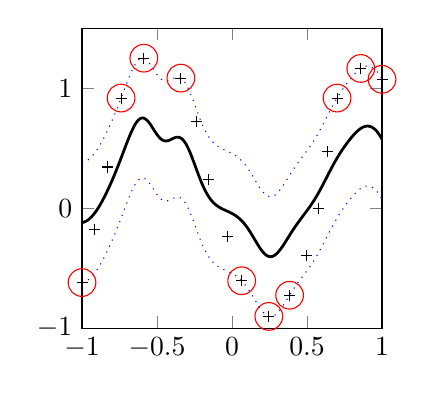
\begin{tikzpicture}

\begin{axis}[%
width=1.5in,
height=1.5in,
scale only axis,
xmin=-1,
xmax=1,
ymin=-1,
ymax=1.5,
]
\addplot [color=black,solid,line width=1.0pt,forget plot]
  table[row sep=crcr]{%
-1	-0.119455645186418\\
-0.993333333333333	-0.117782315701881\\
-0.986666666666667	-0.115330439070124\\
-0.98	-0.112085410918312\\
-0.973333333333333	-0.108038333412802\\
-0.966666666666667	-0.103185792949165\\
-0.96	-0.0975295395652418\\
-0.953333333333333	-0.091076083602175\\
-0.946666666666667	-0.0838362270005101\\
-0.94	-0.075824547580335\\
-0.933333333333333	-0.0670588546991235\\
-0.926666666666667	-0.057559633847747\\
-0.92	-0.0473494961282862\\
-0.913333333333333	-0.0364526463011332\\
-0.906666666666667	-0.0248943803794624\\
-0.9	-0.01270062080266\\
-0.893333333333333	0.000102505730774013\\
-0.886666666666667	0.0134890454130289\\
-0.88	0.0274335493789692\\
-0.873333333333333	0.0419113622268442\\
-0.866666666666667	0.0568988694534322\\
-0.86	0.0723737062824397\\
-0.853333333333333	0.0883149295425906\\
-0.846666666666667	0.104703152638042\\
-0.84	0.121520641386153\\
-0.833333333333333	0.138751365782292\\
-0.826666666666667	0.156380999852549\\
-0.82	0.174396858980029\\
-0.813333333333333	0.19278776176988\\
-0.806666666666667	0.211543801984328\\
-0.8	0.230656015640675\\
-0.793333333333333	0.250115929283309\\
-0.786666666666667	0.26991497790457\\
-0.78	0.290043785095808\\
-0.773333333333333	0.310491303747913\\
-0.766666666666667	0.331243822860176\\
-0.76	0.352283854506237\\
-0.753333333333333	0.373588924377962\\
-0.746666666666667	0.395130299110457\\
-0.74	0.416871693228989\\
-0.733333333333333	0.438768007441051\\
-0.726666666666667	0.460764157492252\\
-0.72	0.482794058297092\\
-0.713333333333333	0.504779830984181\\
-0.706666666666667	0.526631300393405\\
-0.7	0.548245847092743\\
-0.693333333333333	0.569508670967361\\
-0.686666666666667	0.590293512877499\\
-0.68	0.610463866983062\\
-0.673333333333333	0.629874699486165\\
-0.666666666666667	0.648374670328512\\
-0.66	0.665808833543377\\
-0.653333333333333	0.68202177037964\\
-0.646666666666667	0.696861087956775\\
-0.64	0.710181196087799\\
-0.633333333333333	0.721847257026299\\
-0.626666666666667	0.73173918819677\\
-0.62	0.739755587284916\\
-0.613333333333333	0.745817443067874\\
-0.606666666666667	0.749871494528023\\
-0.6	0.751893105367408\\
-0.593333333333333	0.751888531030694\\
-0.586666666666667	0.749896470515271\\
-0.58	0.745988815124161\\
-0.573333333333333	0.740270530212236\\
-0.566666666666667	0.732878633017899\\
-0.56	0.723980258848051\\
-0.553333333333333	0.713769838086412\\
-0.546666666666667	0.702465436573026\\
-0.54	0.690304340712338\\
-0.533333333333333	0.677537995122203\\
-0.526666666666667	0.664426423751577\\
-0.52	0.651232284326113\\
-0.513333333333333	0.638214720054022\\
-0.506666666666667	0.625623181257031\\
-0.5	0.613691392704012\\
-0.493333333333333	0.602631639845737\\
-0.486666666666667	0.592629539006687\\
-0.48	0.583839443201083\\
-0.473333333333333	0.576380617091588\\
-0.466666666666667	0.570334292333024\\
-0.46	0.565741688892053\\
-0.453333333333333	0.562603059750499\\
-0.446666666666667	0.560877786590215\\
-0.44	0.560485523559982\\
-0.433333333333333	0.561308355983594\\
-0.426666666666667	0.563193911805313\\
-0.42	0.565959336559459\\
-0.413333333333333	0.569396018500052\\
-0.406666666666667	0.573274929947028\\
-0.4	0.577352434499204\\
-0.393333333333333	0.581376398004014\\
-0.386666666666667	0.585092434390099\\
-0.38	0.588250115837417\\
-0.373333333333333	0.590608980295124\\
-0.366666666666667	0.591944177910489\\
-0.36	0.59205161119024\\
-0.353333333333333	0.59075244121201\\
-0.346666666666667	0.58789685332892\\
-0.34	0.583366999833418\\
-0.333333333333333	0.577079063137188\\
-0.326666666666667	0.568984410283569\\
-0.32	0.559069837102688\\
-0.313333333333333	0.547356927112577\\
-0.306666666666667	0.533900575463401\\
-0.3	0.518786750989972\\
-0.293333333333333	0.502129589058734\\
-0.286666666666667	0.484067923781589\\
-0.28	0.464761379889162\\
-0.273333333333333	0.44438615185095\\
-0.266666666666667	0.423130600619132\\
-0.26	0.401190796754664\\
-0.253333333333333	0.378766132935151\\
-0.246666666666667	0.356055119361915\\
-0.24	0.333251462923946\\
-0.233333333333333	0.310540515782379\\
-0.226666666666667	0.288096162019318\\
-0.22	0.266078192888303\\
-0.213333333333333	0.244630202745744\\
-0.206666666666667	0.223878019632282\\
-0.2	0.203928667344473\\
-0.193333333333333	0.184869840236246\\
-0.186666666666667	0.166769858355629\\
-0.18	0.149678059177721\\
-0.173333333333333	0.133625573340254\\
-0.166666666666667	0.118626425504298\\
-0.16	0.104678897718808\\
-0.153333333333333	0.0917670913338046\\
-0.146666666666667	0.0798626243704002\\
-0.14	0.0689264040407239\\
-0.133333333333333	0.0589104184974292\\
-0.126666666666667	0.0497594975386065\\
-0.12	0.0414129985527661\\
-0.113333333333333	0.033806381126231\\
-0.106666666666667	0.026872641144493\\
-0.1	0.0205435826297871\\
-0.0933333333333333	0.0147509127434772\\
-0.0866666666666666	0.00942715216551302\\
-0.08	0.00450635931335585\\
-0.0733333333333333	-7.53275069385247e-05\\
-0.0666666666666667	-0.00437932096168202\\
-0.0599999999999999	-0.00846437522626724\\
-0.0533333333333332	-0.012386519255251\\
-0.0466666666666666	-0.016199112888494\\
-0.0399999999999999	-0.019953003562107\\
-0.0333333333333333	-0.0236967596502722\\
-0.0266666666666666	-0.0274769552890359\\
-0.0199999999999999	-0.0313384809125136\\
-0.0133333333333333	-0.0353248536643514\\
-0.0066666666666666	-0.039478502343322\\
1.11022302462516e-16	-0.0438410026217969\\
0.00666666666666682	-0.048453239965113\\
0.0133333333333335	-0.0533554800038981\\
0.0200000000000001	-0.0585873290885842\\
0.0266666666666668	-0.0641875713896833\\
0.0333333333333335	-0.0701938731815121\\
0.0400000000000001	-0.0766423498154645\\
0.0466666666666669	-0.0835669962728895\\
0.0533333333333335	-0.0909989879716797\\
0.0600000000000002	-0.0989658645315155\\
0.0666666666666669	-0.107490615290716\\
0.0733333333333335	-0.11659069129129\\
0.0800000000000002	-0.126276973961771\\
0.0866666666666668	-0.136552735568586\\
0.0933333333333335	-0.147412630412485\\
0.1	-0.158841758464281\\
0.106666666666667	-0.170814844438098\\
0.113333333333334	-0.183295575005668\\
0.12	-0.196236134833465\\
0.126666666666667	-0.209576978315352\\
0.133333333333334	-0.223246868295215\\
0.14	-0.237163205829566\\
0.146666666666667	-0.251232666318994\\
0.153333333333334	-0.265352147413087\\
0.16	-0.279410023315757\\
0.166666666666667	-0.293287688900044\\
0.173333333333333	-0.306861365843147\\
0.18	-0.320004132298875\\
0.186666666666667	-0.332588127923231\\
0.193333333333333	-0.344486877823518\\
0.2	-0.355577672628233\\
0.206666666666667	-0.365743937718119\\
0.213333333333333	-0.374877522969758\\
0.22	-0.382880845284468\\
0.226666666666667	-0.38966881973005\\
0.233333333333334	-0.395170521209322\\
0.24	-0.399330526963874\\
0.246666666666667	-0.402109900587271\\
0.253333333333334	-0.403486790125066\\
0.26	-0.403456625769356\\
0.266666666666667	-0.402031916053096\\
0.273333333333334	-0.399241654732547\\
0.28	-0.395130363142559\\
0.286666666666667	-0.389756804185485\\
0.293333333333334	-0.383192413802803\\
0.3	-0.375519503401868\\
0.306666666666667	-0.366829291999517\\
0.313333333333333	-0.357219829650788\\
0.32	-0.346793874031548\\
0.326666666666667	-0.335656779938179\\
0.333333333333333	-0.32391445716986\\
0.34	-0.311671446082329\\
0.346666666666667	-0.299029152438093\\
0.353333333333333	-0.286084274472674\\
0.36	-0.272927445823898\\
0.366666666666667	-0.259642108606388\\
0.373333333333334	-0.246303621906713\\
0.38	-0.23297860272834\\
0.386666666666667	-0.219724489264122\\
0.393333333333334	-0.2065893105698\\
0.4	-0.193611642415562\\
0.406666666666667	-0.180820726369247\\
0.413333333333334	-0.168236727986531\\
0.42	-0.155871110236275\\
0.426666666666667	-0.14372709978475\\
0.433333333333334	-0.13180022625309\\
0.44	-0.120078917758941\\
0.446666666666667	-0.108545139644633\\
0.453333333333333	-0.0971750669658272\\
0.46	-0.0859397847678603\\
0.466666666666667	-0.0748060131455951\\
0.473333333333333	-0.0637368563468336\\
0.48	-0.0526925765775723\\
0.486666666666667	-0.0416313936033107\\
0.493333333333334	-0.0305103106874898\\
0.5	-0.0192859659088004\\
0.506666666666667	-0.00791550556255729\\
0.513333333333334	0.00364252665392176\\
0.52	0.0154272944278601\\
0.526666666666667	0.0274747809962504\\
0.533333333333334	0.0398169256633196\\
0.54	0.052480804839584\\
0.546666666666667	0.0654878803178186\\
0.553333333333333	0.0788533391427194\\
0.56	0.0925855499527725\\
0.566666666666667	0.106685659912984\\
0.573333333333333	0.121147354218852\\
0.58	0.135956796612448\\
0.586666666666667	0.151092764467514\\
0.593333333333333	0.166526985910058\\
0.6	0.182224679360812\\
0.606666666666667	0.198145288104737\\
0.613333333333334	0.214243394359575\\
0.62	0.230469789224617\\
0.626666666666667	0.246772667262835\\
0.633333333333334	0.263098907729213\\
0.64	0.279395399011366\\
0.646666666666667	0.295610359057875\\
0.653333333333334	0.311694602731365\\
0.66	0.327602707345628\\
0.666666666666667	0.343294030232874\\
0.673333333333334	0.358733537024888\\
0.68	0.373892406283911\\
0.686666666666667	0.38874838492615\\
0.693333333333334	0.403285879169928\\
0.7	0.41749577703963\\
0.706666666666667	0.431375010218186\\
0.713333333333334	0.444925874669432\\
0.72	0.458155140337119\\
0.726666666666667	0.471072989779814\\
0.733333333333334	0.483691833287046\\
0.74	0.496025053398214\\
0.746666666666667	0.508085734488526\\
0.753333333333334	0.519885433014964\\
0.76	0.531433041108075\\
0.766666666666667	0.542733790594668\\
0.773333333333334	0.553788436544347\\
0.78	0.564592649496857\\
0.786666666666667	0.57513663421551\\
0.793333333333334	0.585404980780561\\
0.8	0.595376741789799\\
0.806666666666667	0.605025718081221\\
0.813333333333334	0.614320925404148\\
0.82	0.623227206427373\\
0.826666666666667	0.631705946851464\\
0.833333333333333	0.639715851500517\\
0.84	0.647213736245744\\
0.846666666666667	0.654155294414668\\
0.853333333333333	0.660495801738131\\
0.86	0.666190731487306\\
0.866666666666667	0.671196260715724\\
0.873333333333334	0.67546965880019\\
0.88	0.678969560057188\\
0.886666666666667	0.681656132367196\\
0.893333333333334	0.683491162768021\\
0.9	0.684438088256166\\
0.906666666666667	0.684462005057513\\
0.913333333333334	0.683529692042348\\
0.92	0.681609683587682\\
0.926666666666667	0.678672424041594\\
0.933333333333334	0.67469053021575\\
0.94	0.669639180391259\\
0.946666666666667	0.663496638685388\\
0.953333333333334	0.656244912920512\\
0.96	0.647870533061431\\
0.966666666666667	0.638365426566807\\
0.973333333333334	0.627727857336638\\
0.98	0.615963386964431\\
0.986666666666667	0.603085811246548\\
0.993333333333334	0.589118021748848\\
1	0.574092741906371\\
};
\addplot [color=blue,dotted,forget plot]
  table[row sep=crcr]{%
-1	0.380544354813582\\
-0.993333333333333	0.382217684298119\\
-0.986666666666667	0.384669560929876\\
-0.98	0.387914589081688\\
-0.973333333333333	0.391961666587198\\
-0.966666666666667	0.396814207050835\\
-0.96	0.402470460434758\\
-0.953333333333333	0.408923916397825\\
-0.946666666666667	0.41616377299949\\
-0.94	0.424175452419665\\
-0.933333333333333	0.432941145300877\\
-0.926666666666667	0.442440366152253\\
-0.92	0.452650503871714\\
-0.913333333333333	0.463547353698867\\
-0.906666666666667	0.475105619620538\\
-0.9	0.48729937919734\\
-0.893333333333333	0.500102505730774\\
-0.886666666666667	0.513489045413029\\
-0.88	0.527433549378969\\
-0.873333333333333	0.541911362226844\\
-0.866666666666667	0.556898869453432\\
-0.86	0.57237370628244\\
-0.853333333333333	0.588314929542591\\
-0.846666666666667	0.604703152638042\\
-0.84	0.621520641386153\\
-0.833333333333333	0.638751365782292\\
-0.826666666666667	0.656380999852549\\
-0.82	0.674396858980029\\
-0.813333333333333	0.69278776176988\\
-0.806666666666667	0.711543801984328\\
-0.8	0.730656015640675\\
-0.793333333333333	0.750115929283309\\
-0.786666666666667	0.76991497790457\\
-0.78	0.790043785095808\\
-0.773333333333333	0.810491303747913\\
-0.766666666666667	0.831243822860176\\
-0.76	0.852283854506237\\
-0.753333333333333	0.873588924377962\\
-0.746666666666667	0.895130299110457\\
-0.74	0.91687169322899\\
-0.733333333333333	0.93876800744105\\
-0.726666666666667	0.960764157492252\\
-0.72	0.982794058297092\\
-0.713333333333333	1.00477983098418\\
-0.706666666666667	1.02663130039341\\
-0.7	1.04824584709274\\
-0.693333333333333	1.06950867096736\\
-0.686666666666667	1.0902935128775\\
-0.68	1.11046386698306\\
-0.673333333333333	1.12987469948617\\
-0.666666666666667	1.14837467032851\\
-0.66	1.16580883354338\\
-0.653333333333333	1.18202177037964\\
-0.646666666666667	1.19686108795677\\
-0.64	1.2101811960878\\
-0.633333333333333	1.2218472570263\\
-0.626666666666667	1.23173918819677\\
-0.62	1.23975558728492\\
-0.613333333333333	1.24581744306787\\
-0.606666666666667	1.24987149452802\\
-0.6	1.25189310536741\\
-0.593333333333333	1.25188853103069\\
-0.586666666666667	1.24989647051527\\
-0.58	1.24598881512416\\
-0.573333333333333	1.24027053021224\\
-0.566666666666667	1.2328786330179\\
-0.56	1.22398025884805\\
-0.553333333333333	1.21376983808641\\
-0.546666666666667	1.20246543657303\\
-0.54	1.19030434071234\\
-0.533333333333333	1.1775379951222\\
-0.526666666666667	1.16442642375158\\
-0.52	1.15123228432611\\
-0.513333333333333	1.13821472005402\\
-0.506666666666667	1.12562318125703\\
-0.5	1.11369139270401\\
-0.493333333333333	1.10263163984574\\
-0.486666666666667	1.09262953900669\\
-0.48	1.08383944320108\\
-0.473333333333333	1.07638061709159\\
-0.466666666666667	1.07033429233302\\
-0.46	1.06574168889205\\
-0.453333333333333	1.0626030597505\\
-0.446666666666667	1.06087778659022\\
-0.44	1.06048552355998\\
-0.433333333333333	1.06130835598359\\
-0.426666666666667	1.06319391180531\\
-0.42	1.06595933655946\\
-0.413333333333333	1.06939601850005\\
-0.406666666666667	1.07327492994703\\
-0.4	1.0773524344992\\
-0.393333333333333	1.08137639800401\\
-0.386666666666667	1.0850924343901\\
-0.38	1.08825011583742\\
-0.373333333333333	1.09060898029512\\
-0.366666666666667	1.09194417791049\\
-0.36	1.09205161119024\\
-0.353333333333333	1.09075244121201\\
-0.346666666666667	1.08789685332892\\
-0.34	1.08336699983342\\
-0.333333333333333	1.07707906313719\\
-0.326666666666667	1.06898441028357\\
-0.32	1.05906983710269\\
-0.313333333333333	1.04735692711258\\
-0.306666666666667	1.0339005754634\\
-0.3	1.01878675098997\\
-0.293333333333333	1.00212958905873\\
-0.286666666666667	0.984067923781589\\
-0.28	0.964761379889162\\
-0.273333333333333	0.94438615185095\\
-0.266666666666667	0.923130600619132\\
-0.26	0.901190796754664\\
-0.253333333333333	0.878766132935151\\
-0.246666666666667	0.856055119361915\\
-0.24	0.833251462923946\\
-0.233333333333333	0.810540515782379\\
-0.226666666666667	0.788096162019318\\
-0.22	0.766078192888303\\
-0.213333333333333	0.744630202745745\\
-0.206666666666667	0.723878019632282\\
-0.2	0.703928667344473\\
-0.193333333333333	0.684869840236246\\
-0.186666666666667	0.666769858355629\\
-0.18	0.649678059177721\\
-0.173333333333333	0.633625573340254\\
-0.166666666666667	0.618626425504298\\
-0.16	0.604678897718808\\
-0.153333333333333	0.591767091333805\\
-0.146666666666667	0.5798626243704\\
-0.14	0.568926404040724\\
-0.133333333333333	0.558910418497429\\
-0.126666666666667	0.549759497538606\\
-0.12	0.541412998552766\\
-0.113333333333333	0.533806381126231\\
-0.106666666666667	0.526872641144493\\
-0.1	0.520543582629787\\
-0.0933333333333333	0.514750912743477\\
-0.0866666666666666	0.509427152165513\\
-0.08	0.504506359313356\\
-0.0733333333333333	0.499924672493061\\
-0.0666666666666667	0.495620679038318\\
-0.0599999999999999	0.491535624773733\\
-0.0533333333333332	0.487613480744749\\
-0.0466666666666666	0.483800887111506\\
-0.0399999999999999	0.480046996437893\\
-0.0333333333333333	0.476303240349728\\
-0.0266666666666666	0.472523044710964\\
-0.0199999999999999	0.468661519087486\\
-0.0133333333333333	0.464675146335649\\
-0.0066666666666666	0.460521497656678\\
1.11022302462516e-16	0.456158997378203\\
0.00666666666666682	0.451546760034887\\
0.0133333333333335	0.446644519996102\\
0.0200000000000001	0.441412670911416\\
0.0266666666666668	0.435812428610317\\
0.0333333333333335	0.429806126818488\\
0.0400000000000001	0.423357650184535\\
0.0466666666666669	0.41643300372711\\
0.0533333333333335	0.40900101202832\\
0.0600000000000002	0.401034135468485\\
0.0666666666666669	0.392509384709284\\
0.0733333333333335	0.38340930870871\\
0.0800000000000002	0.373723026038229\\
0.0866666666666668	0.363447264431414\\
0.0933333333333335	0.352587369587515\\
0.1	0.341158241535719\\
0.106666666666667	0.329185155561902\\
0.113333333333334	0.316704424994331\\
0.12	0.303763865166535\\
0.126666666666667	0.290423021684648\\
0.133333333333334	0.276753131704785\\
0.14	0.262836794170434\\
0.146666666666667	0.248767333681006\\
0.153333333333334	0.234647852586913\\
0.16	0.220589976684243\\
0.166666666666667	0.206712311099956\\
0.173333333333333	0.193138634156853\\
0.18	0.179995867701125\\
0.186666666666667	0.167411872076769\\
0.193333333333333	0.155513122176482\\
0.2	0.144422327371767\\
0.206666666666667	0.134256062281881\\
0.213333333333333	0.125122477030242\\
0.22	0.117119154715532\\
0.226666666666667	0.11033118026995\\
0.233333333333334	0.104829478790678\\
0.24	0.100669473036126\\
0.246666666666667	0.0978900994127292\\
0.253333333333334	0.0965132098749337\\
0.26	0.0965433742306445\\
0.266666666666667	0.0979680839469035\\
0.273333333333334	0.100758345267453\\
0.28	0.104869636857441\\
0.286666666666667	0.110243195814515\\
0.293333333333334	0.116807586197197\\
0.3	0.124480496598132\\
0.306666666666667	0.133170708000483\\
0.313333333333333	0.142780170349212\\
0.32	0.153206125968452\\
0.326666666666667	0.164343220061821\\
0.333333333333333	0.17608554283014\\
0.34	0.188328553917671\\
0.346666666666667	0.200970847561907\\
0.353333333333333	0.213915725527326\\
0.36	0.227072554176102\\
0.366666666666667	0.240357891393612\\
0.373333333333334	0.253696378093287\\
0.38	0.26702139727166\\
0.386666666666667	0.280275510735878\\
0.393333333333334	0.2934106894302\\
0.4	0.306388357584438\\
0.406666666666667	0.319179273630753\\
0.413333333333334	0.331763272013469\\
0.42	0.344128889763725\\
0.426666666666667	0.35627290021525\\
0.433333333333334	0.36819977374691\\
0.44	0.379921082241059\\
0.446666666666667	0.391454860355367\\
0.453333333333333	0.402824933034173\\
0.46	0.41406021523214\\
0.466666666666667	0.425193986854405\\
0.473333333333333	0.436263143653166\\
0.48	0.447307423422428\\
0.486666666666667	0.458368606396689\\
0.493333333333334	0.46948968931251\\
0.5	0.4807140340912\\
0.506666666666667	0.492084494437443\\
0.513333333333334	0.503642526653922\\
0.52	0.51542729442786\\
0.526666666666667	0.52747478099625\\
0.533333333333334	0.53981692566332\\
0.54	0.552480804839584\\
0.546666666666667	0.565487880317819\\
0.553333333333333	0.578853339142719\\
0.56	0.592585549952773\\
0.566666666666667	0.606685659912984\\
0.573333333333333	0.621147354218852\\
0.58	0.635956796612448\\
0.586666666666667	0.651092764467514\\
0.593333333333333	0.666526985910058\\
0.6	0.682224679360812\\
0.606666666666667	0.698145288104737\\
0.613333333333334	0.714243394359575\\
0.62	0.730469789224617\\
0.626666666666667	0.746772667262835\\
0.633333333333334	0.763098907729213\\
0.64	0.779395399011366\\
0.646666666666667	0.795610359057875\\
0.653333333333334	0.811694602731365\\
0.66	0.827602707345628\\
0.666666666666667	0.843294030232874\\
0.673333333333334	0.858733537024888\\
0.68	0.873892406283911\\
0.686666666666667	0.88874838492615\\
0.693333333333334	0.903285879169928\\
0.7	0.91749577703963\\
0.706666666666667	0.931375010218186\\
0.713333333333334	0.944925874669432\\
0.72	0.958155140337119\\
0.726666666666667	0.971072989779814\\
0.733333333333334	0.983691833287046\\
0.74	0.996025053398214\\
0.746666666666667	1.00808573448853\\
0.753333333333334	1.01988543301496\\
0.76	1.03143304110808\\
0.766666666666667	1.04273379059467\\
0.773333333333334	1.05378843654435\\
0.78	1.06459264949686\\
0.786666666666667	1.07513663421551\\
0.793333333333334	1.08540498078056\\
0.8	1.0953767417898\\
0.806666666666667	1.10502571808122\\
0.813333333333334	1.11432092540415\\
0.82	1.12322720642737\\
0.826666666666667	1.13170594685146\\
0.833333333333333	1.13971585150052\\
0.84	1.14721373624574\\
0.846666666666667	1.15415529441467\\
0.853333333333333	1.16049580173813\\
0.86	1.16619073148731\\
0.866666666666667	1.17119626071572\\
0.873333333333334	1.17546965880019\\
0.88	1.17896956005719\\
0.886666666666667	1.1816561323672\\
0.893333333333334	1.18349116276802\\
0.9	1.18443808825617\\
0.906666666666667	1.18446200505751\\
0.913333333333334	1.18352969204235\\
0.92	1.18160968358768\\
0.926666666666667	1.17867242404159\\
0.933333333333334	1.17469053021575\\
0.94	1.16963918039126\\
0.946666666666667	1.16349663868539\\
0.953333333333334	1.15624491292051\\
0.96	1.14787053306143\\
0.966666666666667	1.13836542656681\\
0.973333333333334	1.12772785733664\\
0.98	1.11596338696443\\
0.986666666666667	1.10308581124655\\
0.993333333333334	1.08911802174885\\
1	1.07409274190637\\
};
\addplot [color=blue,dotted,forget plot]
  table[row sep=crcr]{%
-1	-0.619455645186418\\
-0.993333333333333	-0.617782315701881\\
-0.986666666666667	-0.615330439070124\\
-0.98	-0.612085410918312\\
-0.973333333333333	-0.608038333412802\\
-0.966666666666667	-0.603185792949165\\
-0.96	-0.597529539565242\\
-0.953333333333333	-0.591076083602175\\
-0.946666666666667	-0.58383622700051\\
-0.94	-0.575824547580335\\
-0.933333333333333	-0.567058854699124\\
-0.926666666666667	-0.557559633847747\\
-0.92	-0.547349496128286\\
-0.913333333333333	-0.536452646301133\\
-0.906666666666667	-0.524894380379462\\
-0.9	-0.51270062080266\\
-0.893333333333333	-0.499897494269226\\
-0.886666666666667	-0.486510954586971\\
-0.88	-0.472566450621031\\
-0.873333333333333	-0.458088637773156\\
-0.866666666666667	-0.443101130546568\\
-0.86	-0.42762629371756\\
-0.853333333333333	-0.411685070457409\\
-0.846666666666667	-0.395296847361958\\
-0.84	-0.378479358613847\\
-0.833333333333333	-0.361248634217708\\
-0.826666666666667	-0.343619000147451\\
-0.82	-0.325603141019971\\
-0.813333333333333	-0.30721223823012\\
-0.806666666666667	-0.288456198015672\\
-0.8	-0.269343984359325\\
-0.793333333333333	-0.249884070716691\\
-0.786666666666667	-0.23008502209543\\
-0.78	-0.209956214904192\\
-0.773333333333333	-0.189508696252087\\
-0.766666666666667	-0.168756177139824\\
-0.76	-0.147716145493763\\
-0.753333333333333	-0.126411075622038\\
-0.746666666666667	-0.104869700889543\\
-0.74	-0.0831283067710105\\
-0.733333333333333	-0.0612319925589495\\
-0.726666666666667	-0.0392358425077485\\
-0.72	-0.017205941702908\\
-0.713333333333333	0.00477983098418133\\
-0.706666666666667	0.0266313003934053\\
-0.7	0.0482458470927433\\
-0.693333333333333	0.069508670967361\\
-0.686666666666667	0.0902935128774985\\
-0.68	0.110463866983062\\
-0.673333333333333	0.129874699486165\\
-0.666666666666667	0.148374670328512\\
-0.66	0.165808833543377\\
-0.653333333333333	0.18202177037964\\
-0.646666666666667	0.196861087956775\\
-0.64	0.210181196087799\\
-0.633333333333333	0.221847257026299\\
-0.626666666666667	0.23173918819677\\
-0.62	0.239755587284916\\
-0.613333333333333	0.245817443067874\\
-0.606666666666667	0.249871494528023\\
-0.6	0.251893105367408\\
-0.593333333333333	0.251888531030694\\
-0.586666666666667	0.249896470515271\\
-0.58	0.245988815124161\\
-0.573333333333333	0.240270530212236\\
-0.566666666666667	0.232878633017899\\
-0.56	0.223980258848051\\
-0.553333333333333	0.213769838086412\\
-0.546666666666667	0.202465436573026\\
-0.54	0.190304340712338\\
-0.533333333333333	0.177537995122203\\
-0.526666666666667	0.164426423751577\\
-0.52	0.151232284326113\\
-0.513333333333333	0.138214720054022\\
-0.506666666666667	0.125623181257031\\
-0.5	0.113691392704012\\
-0.493333333333333	0.102631639845737\\
-0.486666666666667	0.092629539006687\\
-0.48	0.0838394432010826\\
-0.473333333333333	0.0763806170915878\\
-0.466666666666667	0.0703342923330237\\
-0.46	0.0657416888920531\\
-0.453333333333333	0.0626030597504994\\
-0.446666666666667	0.0608777865902153\\
-0.44	0.0604855235599816\\
-0.433333333333333	0.061308355983594\\
-0.426666666666667	0.0631939118053134\\
-0.42	0.0659593365594591\\
-0.413333333333333	0.0693960185000522\\
-0.406666666666667	0.0732749299470277\\
-0.4	0.0773524344992043\\
-0.393333333333333	0.0813763980040139\\
-0.386666666666667	0.0850924343900987\\
-0.38	0.0882501158374168\\
-0.373333333333333	0.0906089802951244\\
-0.366666666666667	0.0919441779104887\\
-0.36	0.0920516111902403\\
-0.353333333333333	0.0907524412120104\\
-0.346666666666667	0.0878968533289203\\
-0.34	0.0833669998334177\\
-0.333333333333333	0.0770790631371876\\
-0.326666666666667	0.0689844102835695\\
-0.32	0.0590698371026884\\
-0.313333333333333	0.0473569271125772\\
-0.306666666666667	0.033900575463401\\
-0.3	0.0187867509899718\\
-0.293333333333333	0.00212958905873384\\
-0.286666666666667	-0.0159320762184114\\
-0.28	-0.0352386201108378\\
-0.273333333333333	-0.0556138481490497\\
-0.266666666666667	-0.0768693993808683\\
-0.26	-0.0988092032453363\\
-0.253333333333333	-0.121233867064849\\
-0.246666666666667	-0.143944880638085\\
-0.24	-0.166748537076054\\
-0.233333333333333	-0.189459484217621\\
-0.226666666666667	-0.211903837980682\\
-0.22	-0.233921807111697\\
-0.213333333333333	-0.255369797254256\\
-0.206666666666667	-0.276121980367718\\
-0.2	-0.296071332655527\\
-0.193333333333333	-0.315130159763754\\
-0.186666666666667	-0.333230141644371\\
-0.18	-0.350321940822279\\
-0.173333333333333	-0.366374426659746\\
-0.166666666666667	-0.381373574495702\\
-0.16	-0.395321102281192\\
-0.153333333333333	-0.408232908666195\\
-0.146666666666667	-0.4201373756296\\
-0.14	-0.431073595959276\\
-0.133333333333333	-0.441089581502571\\
-0.126666666666667	-0.450240502461394\\
-0.12	-0.458587001447234\\
-0.113333333333333	-0.466193618873769\\
-0.106666666666667	-0.473127358855507\\
-0.1	-0.479456417370213\\
-0.0933333333333333	-0.485249087256523\\
-0.0866666666666666	-0.490572847834487\\
-0.08	-0.495493640686644\\
-0.0733333333333333	-0.500075327506939\\
-0.0666666666666667	-0.504379320961682\\
-0.0599999999999999	-0.508464375226267\\
-0.0533333333333332	-0.512386519255251\\
-0.0466666666666666	-0.516199112888494\\
-0.0399999999999999	-0.519953003562107\\
-0.0333333333333333	-0.523696759650272\\
-0.0266666666666666	-0.527476955289036\\
-0.0199999999999999	-0.531338480912514\\
-0.0133333333333333	-0.535324853664351\\
-0.0066666666666666	-0.539478502343322\\
1.11022302462516e-16	-0.543841002621797\\
0.00666666666666682	-0.548453239965113\\
0.0133333333333335	-0.553355480003898\\
0.0200000000000001	-0.558587329088584\\
0.0266666666666668	-0.564187571389683\\
0.0333333333333335	-0.570193873181512\\
0.0400000000000001	-0.576642349815465\\
0.0466666666666669	-0.58356699627289\\
0.0533333333333335	-0.59099898797168\\
0.0600000000000002	-0.598965864531515\\
0.0666666666666669	-0.607490615290716\\
0.0733333333333335	-0.616590691291291\\
0.0800000000000002	-0.626276973961771\\
0.0866666666666668	-0.636552735568586\\
0.0933333333333335	-0.647412630412485\\
0.1	-0.658841758464281\\
0.106666666666667	-0.670814844438098\\
0.113333333333334	-0.683295575005669\\
0.12	-0.696236134833465\\
0.126666666666667	-0.709576978315352\\
0.133333333333334	-0.723246868295215\\
0.14	-0.737163205829566\\
0.146666666666667	-0.751232666318994\\
0.153333333333334	-0.765352147413087\\
0.16	-0.779410023315757\\
0.166666666666667	-0.793287688900044\\
0.173333333333333	-0.806861365843147\\
0.18	-0.820004132298875\\
0.186666666666667	-0.832588127923231\\
0.193333333333333	-0.844486877823518\\
0.2	-0.855577672628233\\
0.206666666666667	-0.865743937718119\\
0.213333333333333	-0.874877522969758\\
0.22	-0.882880845284468\\
0.226666666666667	-0.88966881973005\\
0.233333333333334	-0.895170521209322\\
0.24	-0.899330526963874\\
0.246666666666667	-0.902109900587271\\
0.253333333333334	-0.903486790125066\\
0.26	-0.903456625769355\\
0.266666666666667	-0.902031916053097\\
0.273333333333334	-0.899241654732547\\
0.28	-0.895130363142558\\
0.286666666666667	-0.889756804185485\\
0.293333333333334	-0.883192413802803\\
0.3	-0.875519503401868\\
0.306666666666667	-0.866829291999517\\
0.313333333333333	-0.857219829650788\\
0.32	-0.846793874031548\\
0.326666666666667	-0.83565677993818\\
0.333333333333333	-0.82391445716986\\
0.34	-0.811671446082329\\
0.346666666666667	-0.799029152438093\\
0.353333333333333	-0.786084274472674\\
0.36	-0.772927445823898\\
0.366666666666667	-0.759642108606388\\
0.373333333333334	-0.746303621906713\\
0.38	-0.73297860272834\\
0.386666666666667	-0.719724489264122\\
0.393333333333334	-0.7065893105698\\
0.4	-0.693611642415562\\
0.406666666666667	-0.680820726369247\\
0.413333333333334	-0.668236727986531\\
0.42	-0.655871110236275\\
0.426666666666667	-0.64372709978475\\
0.433333333333334	-0.63180022625309\\
0.44	-0.620078917758941\\
0.446666666666667	-0.608545139644633\\
0.453333333333333	-0.597175066965827\\
0.46	-0.58593978476786\\
0.466666666666667	-0.574806013145595\\
0.473333333333333	-0.563736856346834\\
0.48	-0.552692576577572\\
0.486666666666667	-0.541631393603311\\
0.493333333333334	-0.53051031068749\\
0.5	-0.5192859659088\\
0.506666666666667	-0.507915505562557\\
0.513333333333334	-0.496357473346078\\
0.52	-0.48457270557214\\
0.526666666666667	-0.47252521900375\\
0.533333333333334	-0.46018307433668\\
0.54	-0.447519195160416\\
0.546666666666667	-0.434512119682181\\
0.553333333333333	-0.421146660857281\\
0.56	-0.407414450047227\\
0.566666666666667	-0.393314340087016\\
0.573333333333333	-0.378852645781148\\
0.58	-0.364043203387552\\
0.586666666666667	-0.348907235532486\\
0.593333333333333	-0.333473014089942\\
0.6	-0.317775320639188\\
0.606666666666667	-0.301854711895263\\
0.613333333333334	-0.285756605640425\\
0.62	-0.269530210775383\\
0.626666666666667	-0.253227332737165\\
0.633333333333334	-0.236901092270787\\
0.64	-0.220604600988634\\
0.646666666666667	-0.204389640942125\\
0.653333333333334	-0.188305397268635\\
0.66	-0.172397292654372\\
0.666666666666667	-0.156705969767126\\
0.673333333333334	-0.141266462975112\\
0.68	-0.126107593716089\\
0.686666666666667	-0.11125161507385\\
0.693333333333334	-0.096714120830072\\
0.7	-0.0825042229603701\\
0.706666666666667	-0.0686249897818144\\
0.713333333333334	-0.055074125330568\\
0.72	-0.0418448596628813\\
0.726666666666667	-0.0289270102201855\\
0.733333333333334	-0.0163081667129535\\
0.74	-0.00397494660178643\\
0.746666666666667	0.00808573448852601\\
0.753333333333334	0.0198854330149638\\
0.76	0.0314330411080752\\
0.766666666666667	0.0427337905946682\\
0.773333333333334	0.053788436544347\\
0.78	0.0645926494968569\\
0.786666666666667	0.0751366342155102\\
0.793333333333334	0.0854049807805614\\
0.8	0.095376741789799\\
0.806666666666667	0.105025718081221\\
0.813333333333334	0.114320925404148\\
0.82	0.123227206427373\\
0.826666666666667	0.131705946851464\\
0.833333333333333	0.139715851500517\\
0.84	0.147213736245744\\
0.846666666666667	0.154155294414668\\
0.853333333333333	0.160495801738131\\
0.86	0.166190731487306\\
0.866666666666667	0.171196260715724\\
0.873333333333334	0.17546965880019\\
0.88	0.178969560057188\\
0.886666666666667	0.181656132367196\\
0.893333333333334	0.183491162768021\\
0.9	0.184438088256166\\
0.906666666666667	0.184462005057513\\
0.913333333333334	0.183529692042348\\
0.92	0.181609683587682\\
0.926666666666667	0.178672424041594\\
0.933333333333334	0.17469053021575\\
0.94	0.169639180391259\\
0.946666666666667	0.163496638685388\\
0.953333333333334	0.156244912920512\\
0.96	0.147870533061431\\
0.966666666666667	0.138365426566807\\
0.973333333333334	0.127727857336638\\
0.98	0.115963386964431\\
0.986666666666667	0.103085811246548\\
0.993333333333334	0.0891180217488478\\
1	0.0740927419063715\\
};
\addplot [color=black,only marks,mark=+,mark options={solid},forget plot]
  table[row sep=crcr]{%
-1	-0.61945564516129\\
};
\addplot [color=red,mark size=5.0pt,only marks,mark=o,mark options={solid},forget plot]
  table[row sep=crcr]{%
-1	-0.61945564516129\\
};
\addplot [color=black,only marks,mark=+,mark options={solid},forget plot]
  table[row sep=crcr]{%
-0.917627677100494	-0.175907258064516\\
};
\addplot [color=black,only marks,mark=+,mark options={solid},forget plot]
  table[row sep=crcr]{%
-0.828665568369028	0.343245967741936\\
};
\addplot [color=black,only marks,mark=+,mark options={solid},forget plot]
  table[row sep=crcr]{%
-0.739703459637562	0.917842741935484\\
};
\addplot [color=red,mark size=5.0pt,only marks,mark=o,mark options={solid},forget plot]
  table[row sep=crcr]{%
-0.739703459637562	0.917842741935484\\
};
\addplot [color=black,only marks,mark=+,mark options={solid},forget plot]
  table[row sep=crcr]{%
-0.588138385502471	1.25050403225806\\
};
\addplot [color=red,mark size=5.0pt,only marks,mark=o,mark options={solid},forget plot]
  table[row sep=crcr]{%
-0.588138385502471	1.25050403225806\\
};
\addplot [color=black,only marks,mark=+,mark options={solid},forget plot]
  table[row sep=crcr]{%
-0.341021416803954	1.08417338709677\\
};
\addplot [color=red,mark size=5.0pt,only marks,mark=o,mark options={solid},forget plot]
  table[row sep=crcr]{%
-0.341021416803954	1.08417338709677\\
};
\addplot [color=black,only marks,mark=+,mark options={solid},forget plot]
  table[row sep=crcr]{%
-0.238879736408567	0.721270161290323\\
};
\addplot [color=black,only marks,mark=+,mark options={solid},forget plot]
  table[row sep=crcr]{%
-0.156507413509061	0.237399193548388\\
};
\addplot [color=black,only marks,mark=+,mark options={solid},forget plot]
  table[row sep=crcr]{%
-0.0280065897858319	-0.236391129032258\\
};
\addplot [color=black,only marks,mark=+,mark options={solid},forget plot]
  table[row sep=crcr]{%
0.0642504118616145	-0.604334677419354\\
};
\addplot [color=red,mark size=5.0pt,only marks,mark=o,mark options={solid},forget plot]
  table[row sep=crcr]{%
0.0642504118616145	-0.604334677419354\\
};
\addplot [color=black,only marks,mark=+,mark options={solid},forget plot]
  table[row sep=crcr]{%
0.245469522240527	-0.901713709677419\\
};
\addplot [color=red,mark size=5.0pt,only marks,mark=o,mark options={solid},forget plot]
  table[row sep=crcr]{%
0.245469522240527	-0.901713709677419\\
};
\addplot [color=black,only marks,mark=+,mark options={solid},forget plot]
  table[row sep=crcr]{%
0.383855024711697	-0.725302419354838\\
};
\addplot [color=red,mark size=5.0pt,only marks,mark=o,mark options={solid},forget plot]
  table[row sep=crcr]{%
0.383855024711697	-0.725302419354838\\
};
\addplot [color=black,only marks,mark=+,mark options={solid},forget plot]
  table[row sep=crcr]{%
0.495881383855025	-0.392641129032258\\
};
\addplot [color=black,only marks,mark=+,mark options={solid},forget plot]
  table[row sep=crcr]{%
0.574958813838551	0.000504032258065168\\
};
\addplot [color=black,only marks,mark=+,mark options={solid},forget plot]
  table[row sep=crcr]{%
0.634266886326194	0.469254032258065\\
};
\addplot [color=black,only marks,mark=+,mark options={solid},forget plot]
  table[row sep=crcr]{%
0.700164744645799	0.917842741935484\\
};
\addplot [color=red,mark size=5.0pt,only marks,mark=o,mark options={solid},forget plot]
  table[row sep=crcr]{%
0.700164744645799	0.917842741935484\\
};
\addplot [color=black,only marks,mark=+,mark options={solid},forget plot]
  table[row sep=crcr]{%
0.85831960461285	1.1648185483871\\
};
\addplot [color=red,mark size=5.0pt,only marks,mark=o,mark options={solid},forget plot]
  table[row sep=crcr]{%
0.85831960461285	1.1648185483871\\
};
\addplot [color=black,only marks,mark=+,mark options={solid},forget plot]
  table[row sep=crcr]{%
1	1.07409274193548\\
};
\addplot [color=red,mark size=5.0pt,only marks,mark=o,mark options={solid},forget plot]
  table[row sep=crcr]{%
1	1.07409274193548\\
};
\end{axis}
\end{tikzpicture}%
\end{document}
\caption{RBF kernel based funtion esimation with $\sigma^2 = 0.1$, $\epsilon = 0.1$, $\epsilon = 0.25$ and $\epsilon = 0.5$.}
\label{fig:ebfEstEps}
\end{figure}
\begin{figure}
\centering
% This file was created by matlab2tikz.
% Minimal pgfplots version: 1.3
%
%The latest updates can be retrieved from
%  http://www.mathworks.com/matlabcentral/fileexchange/22022-matlab2tikz
%where you can also make suggestions and rate matlab2tikz.
%
\documentclass[tikz]{standalone}
\usepackage{pgfplots}
\usepackage{grffile}
\pgfplotsset{compat=newest}
\usetikzlibrary{plotmarks}
\usepackage{amsmath}

\begin{document}
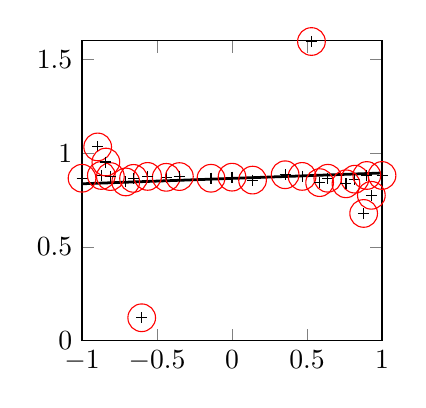
\begin{tikzpicture}

\begin{axis}[%
width=1.5in,
height=1.5in,
scale only axis,
xmin=-1,
xmax=1,
ymin=0,
ymax=1.6,
]
\addplot [color=black,solid,line width=1.0pt,forget plot]
  table[row sep=crcr]{%
-1	0.837249994277954\\
-0.993333333333333	0.837440013885498\\
-0.986666666666667	0.837631940841675\\
-0.98	0.837823987007141\\
-0.973333333333333	0.838015794754028\\
-0.966666666666667	0.838206052780151\\
-0.96	0.838399052619934\\
-0.953333333333333	0.838591694831848\\
-0.946666666666667	0.838783144950867\\
-0.94	0.838975548744202\\
-0.933333333333333	0.839166045188904\\
-0.926666666666667	0.839356899261475\\
-0.92	0.839550018310547\\
-0.913333333333333	0.839741468429565\\
-0.906666666666667	0.839932918548584\\
-0.9	0.840123414993286\\
-0.893333333333333	0.840316414833069\\
-0.886666666666667	0.840508222579956\\
-0.88	0.840698719024658\\
-0.873333333333333	0.840892553329468\\
-0.866666666666667	0.841084241867065\\
-0.86	0.841273903846741\\
-0.853333333333333	0.841467022895813\\
-0.846666666666667	0.841659426689148\\
-0.84	0.841850638389587\\
-0.833333333333333	0.842040181159973\\
-0.826666666666667	0.842234015464783\\
-0.82	0.842426896095276\\
-0.813333333333333	0.842616558074951\\
-0.806666666666667	0.84280800819397\\
-0.8	0.843000292778015\\
-0.793333333333333	0.843191742897034\\
-0.786666666666667	0.843384146690369\\
-0.78	0.843575119972229\\
-0.773333333333333	0.843768000602722\\
-0.766666666666667	0.843960046768188\\
-0.76	0.844151973724365\\
-0.753333333333333	0.844341993331909\\
-0.746666666666667	0.844535350799561\\
-0.74	0.844726920127869\\
-0.733333333333333	0.844918370246887\\
-0.726666666666667	0.845108270645142\\
-0.72	0.845302581787109\\
-0.713333333333333	0.845494151115417\\
-0.706666666666667	0.845685243606567\\
-0.7	0.845876216888428\\
-0.693333333333333	0.846069097518921\\
-0.686666666666667	0.846260190010071\\
-0.68	0.8464515209198\\
-0.673333333333333	0.846644401550293\\
-0.666666666666667	0.846835374832153\\
-0.66	0.847026467323303\\
-0.653333333333333	0.847220182418823\\
-0.646666666666667	0.847411394119263\\
-0.64	0.847602725028992\\
-0.633333333333333	0.847794413566589\\
-0.626666666666667	0.847987055778503\\
-0.62	0.848177075386047\\
-0.613333333333333	0.848368763923645\\
-0.606666666666667	0.848563432693481\\
-0.6	0.848753333091736\\
-0.593333333333333	0.848945379257202\\
-0.586666666666667	0.849136352539062\\
-0.58	0.849329352378845\\
-0.573333333333333	0.849520087242126\\
-0.566666666666667	0.849710881710052\\
-0.56	0.849902927875519\\
-0.553333333333333	0.850095212459564\\
-0.546666666666667	0.85028737783432\\
-0.54	0.850478827953339\\
-0.533333333333333	0.850669205188751\\
-0.526666666666667	0.850863456726074\\
-0.52	0.851053357124329\\
-0.513333333333333	0.851246416568756\\
-0.506666666666667	0.851436614990234\\
-0.5	0.851629853248596\\
-0.493333333333333	0.851821601390839\\
-0.486666666666667	0.852013051509857\\
-0.48	0.852204859256744\\
-0.473333333333333	0.852396428585052\\
-0.466666666666667	0.852588355541229\\
-0.46	0.852779626846313\\
-0.453333333333333	0.852970957756042\\
-0.446666666666667	0.853162586688995\\
-0.44	0.853354513645172\\
-0.433333333333333	0.853546500205994\\
-0.426666666666667	0.853738367557526\\
-0.42	0.853930413722992\\
-0.413333333333333	0.85412186384201\\
-0.406666666666667	0.854313433170319\\
-0.4	0.854504644870758\\
-0.393333333333333	0.854696452617645\\
-0.386666666666667	0.854889094829559\\
-0.38	0.855080842971802\\
-0.373333333333333	0.855272531509399\\
-0.366666666666667	0.855464279651642\\
-0.36	0.855655670166016\\
-0.353333333333333	0.855847716331482\\
-0.346666666666667	0.856038928031921\\
-0.34	0.856230616569519\\
-0.333333333333333	0.856422364711761\\
-0.326666666666667	0.856615424156189\\
-0.32	0.856806218624115\\
-0.313333333333333	0.856998205184937\\
-0.306666666666667	0.857189238071442\\
-0.3	0.857381463050842\\
-0.293333333333333	0.85757303237915\\
-0.286666666666667	0.857764899730682\\
-0.28	0.85795584321022\\
-0.273333333333333	0.858148545026779\\
-0.266666666666667	0.85833939909935\\
-0.26	0.858531892299652\\
-0.253333333333333	0.858723163604736\\
-0.246666666666667	0.858915656805038\\
-0.24	0.859106808900833\\
-0.233333333333333	0.859299063682556\\
-0.226666666666667	0.859490811824799\\
-0.22	0.859682112932205\\
-0.213333333333333	0.859874218702316\\
-0.206666666666667	0.860065788030624\\
-0.2	0.860257178544998\\
-0.193333333333333	0.860449343919754\\
-0.186666666666667	0.860641121864319\\
-0.18	0.860832810401917\\
-0.173333333333333	0.86102432012558\\
-0.166666666666667	0.8612160384655\\
-0.16	0.861407965421677\\
-0.153333333333333	0.86159947514534\\
-0.146666666666667	0.861791342496872\\
-0.14	0.861982792615891\\
-0.133333333333333	0.862174555659294\\
-0.126666666666667	0.862366363406181\\
-0.12	0.862558260560036\\
-0.113333333333333	0.862750023603439\\
-0.106666666666667	0.862941771745682\\
-0.1	0.863133445382118\\
-0.0933333333333333	0.863325208425522\\
-0.0866666666666666	0.863516807556152\\
-0.08	0.863708838820457\\
-0.0733333333333333	0.863900601863861\\
-0.0666666666666667	0.864092133939266\\
-0.0599999999999999	0.864284060895443\\
-0.0533333333333332	0.864475630223751\\
-0.0466666666666666	0.86466746032238\\
-0.0399999999999999	0.864859253168106\\
-0.0333333333333333	0.865050863474607\\
-0.0266666666666666	0.865242671221495\\
-0.0199999999999999	0.865434389561415\\
-0.0133333333333333	0.865626161918044\\
-0.0066666666666666	0.865817894227803\\
0	0.866009637648942\\
0.0066666666666666	0.866201381199062\\
0.0133333333333333	0.866393113508821\\
0.0199999999999999	0.86658488586545\\
0.0266666666666666	0.866776634007692\\
0.0333333333333333	0.866968411952257\\
0.0399999999999999	0.867159992456436\\
0.0466666666666666	0.867351844906807\\
0.0533333333333332	0.867543555796146\\
0.0599999999999999	0.867735244333744\\
0.0666666666666667	0.867927171289921\\
0.0733333333333333	0.868118703365326\\
0.08	0.86831034719944\\
0.0866666666666666	0.868502378463745\\
0.0933333333333333	0.868693977594376\\
0.1	0.868885859847069\\
0.106666666666667	0.869077414274216\\
0.113333333333333	0.869269162416458\\
0.12	0.869460925459862\\
0.126666666666667	0.869652822613716\\
0.133333333333333	0.869844630360603\\
0.14	0.870036393404007\\
0.146666666666667	0.870227843523026\\
0.153333333333333	0.870419949293137\\
0.16	0.870611220598221\\
0.166666666666667	0.870803147554398\\
0.173333333333333	0.870995104312897\\
0.18	0.87118661403656\\
0.186666666666667	0.871378302574158\\
0.193333333333333	0.871570080518723\\
0.2	0.871762007474899\\
0.206666666666667	0.871953397989273\\
0.213333333333333	0.87214520573616\\
0.22	0.872337311506271\\
0.226666666666667	0.872528612613678\\
0.233333333333333	0.87272036075592\\
0.24	0.872912138700485\\
0.246666666666667	0.873103767633438\\
0.253333333333333	0.87329626083374\\
0.26	0.873487293720245\\
0.266666666666667	0.873679786920547\\
0.273333333333333	0.873870879411697\\
0.28	0.874063342809677\\
0.286666666666667	0.874254286289215\\
0.293333333333333	0.874446392059326\\
0.3	0.874637961387634\\
0.306666666666667	0.874830186367035\\
0.313333333333333	0.87502121925354\\
0.32	0.875213205814362\\
0.326666666666667	0.875404000282288\\
0.333333333333333	0.875596582889557\\
0.34	0.875788807868958\\
0.346666666666667	0.875980496406555\\
0.353333333333333	0.876171708106995\\
0.36	0.876363277435303\\
0.366666666666667	0.876555144786835\\
0.373333333333333	0.876746892929077\\
0.38	0.876938581466675\\
0.386666666666667	0.877130329608917\\
0.393333333333333	0.877322971820831\\
0.4	0.87751430273056\\
0.406666666666667	0.877705991268158\\
0.413333333333333	0.877897083759308\\
0.42	0.878089010715485\\
0.426666666666667	0.878281056880951\\
0.433333333333333	0.878472924232483\\
0.44	0.878664910793304\\
0.446666666666667	0.878856837749481\\
0.453333333333333	0.879048466682434\\
0.46	0.879239320755005\\
0.466666666666667	0.879431068897247\\
0.473333333333333	0.879622519016266\\
0.48	0.879814565181732\\
0.486666666666667	0.880006372928619\\
0.493333333333333	0.880197823047638\\
0.5	0.88038957118988\\
0.506666666666667	0.880582809448242\\
0.513333333333333	0.880772531032562\\
0.52	0.880966067314148\\
0.526666666666667	0.881155967712402\\
0.533333333333333	0.881349742412567\\
0.54	0.88154011964798\\
0.546666666666667	0.881732046604156\\
0.553333333333333	0.881924211978912\\
0.56	0.882116496562958\\
0.566666666666667	0.882308542728424\\
0.573333333333333	0.882498860359192\\
0.58	0.882690072059631\\
0.586666666666667	0.882883071899414\\
0.593333333333333	0.883074045181274\\
0.6	0.883266091346741\\
0.606666666666667	0.883455991744995\\
0.613333333333333	0.883650660514832\\
0.62	0.883841395378113\\
0.626666666666667	0.884032368659973\\
0.633333333333333	0.884225010871887\\
0.64	0.884416699409485\\
0.646666666666667	0.884607076644897\\
0.653333333333333	0.884798288345337\\
0.66	0.884992957115173\\
0.666666666666667	0.885184049606323\\
0.673333333333333	0.885375022888184\\
0.68	0.885567903518677\\
0.686666666666667	0.885759234428406\\
0.693333333333333	0.885950326919556\\
0.7	0.886143207550049\\
0.706666666666667	0.886333227157593\\
0.713333333333333	0.886525273323059\\
0.72	0.886716842651367\\
0.726666666666667	0.886911153793335\\
0.733333333333333	0.887101054191589\\
0.74	0.887291550636292\\
0.746666666666667	0.887484073638916\\
0.753333333333333	0.887677431106567\\
0.76	0.887866497039795\\
0.766666666666667	0.888058423995972\\
0.773333333333333	0.888251423835754\\
0.78	0.888443350791931\\
0.786666666666667	0.888635277748108\\
0.793333333333333	0.888826727867126\\
0.8	0.889019131660461\\
0.806666666666667	0.889211416244507\\
0.813333333333333	0.889402866363525\\
0.82	0.889592528343201\\
0.826666666666667	0.889785408973694\\
0.833333333333333	0.889978289604187\\
0.84	0.890168786048889\\
0.846666666666667	0.890359997749329\\
0.853333333333333	0.890551447868347\\
0.86	0.890745520591736\\
0.866666666666667	0.890935182571411\\
0.873333333333333	0.891126871109009\\
0.88	0.891320705413818\\
0.886666666666667	0.891511201858521\\
0.893333333333333	0.891703009605408\\
0.9	0.891895055770874\\
0.906666666666667	0.892086505889893\\
0.913333333333333	0.892277956008911\\
0.92	0.89246940612793\\
0.926666666666667	0.892662525177002\\
0.933333333333333	0.892853379249573\\
0.94	0.893043875694275\\
0.946666666666667	0.89323627948761\\
0.953333333333333	0.893427729606628\\
0.96	0.893620371818542\\
0.966666666666667	0.893813371658325\\
0.973333333333333	0.894003629684448\\
0.98	0.894195437431335\\
0.986666666666667	0.894387483596802\\
0.993333333333333	0.894579410552979\\
1	0.894769430160522\\
};
\addplot [color=black,only marks,mark=+,mark options={solid},forget plot]
  table[row sep=crcr]{%
0.818827708703375	0.861888122983872\\
};
\addplot [color=red,mark size=5.0pt,only marks,mark=o,mark options={solid},forget plot]
  table[row sep=crcr]{%
0.818827708703375	0.861888122983872\\
};
\addplot [color=black,only marks,mark=+,mark options={solid},forget plot]
  table[row sep=crcr]{%
0.136767317939609	0.856960457661291\\
};
\addplot [color=red,mark size=5.0pt,only marks,mark=o,mark options={solid},forget plot]
  table[row sep=crcr]{%
0.136767317939609	0.856960457661291\\
};
\addplot [color=black,only marks,mark=+,mark options={solid},forget plot]
  table[row sep=crcr]{%
-0.438721136767318	0.871743453629032\\
};
\addplot [color=red,mark size=5.0pt,only marks,mark=o,mark options={solid},forget plot]
  table[row sep=crcr]{%
-0.438721136767318	0.871743453629032\\
};
\addplot [color=black,only marks,mark=+,mark options={solid},forget plot]
  table[row sep=crcr]{%
-1	0.866815788306452\\
};
\addplot [color=red,mark size=5.0pt,only marks,mark=o,mark options={solid},forget plot]
  table[row sep=crcr]{%
-1	0.866815788306452\\
};
\addplot [color=black,only marks,mark=+,mark options={solid},forget plot]
  table[row sep=crcr]{%
-0.708703374777975	0.847105127016129\\
};
\addplot [color=red,mark size=5.0pt,only marks,mark=o,mark options={solid},forget plot]
  table[row sep=crcr]{%
-0.708703374777975	0.847105127016129\\
};
\addplot [color=black,only marks,mark=+,mark options={solid},forget plot]
  table[row sep=crcr]{%
-0.140319715808171	0.866815788306452\\
};
\addplot [color=red,mark size=5.0pt,only marks,mark=o,mark options={solid},forget plot]
  table[row sep=crcr]{%
-0.140319715808171	0.866815788306452\\
};
\addplot [color=black,only marks,mark=+,mark options={solid},forget plot]
  table[row sep=crcr]{%
0.467140319715808	0.876671118951613\\
};
\addplot [color=red,mark size=5.0pt,only marks,mark=o,mark options={solid},forget plot]
  table[row sep=crcr]{%
0.467140319715808	0.876671118951613\\
};
\addplot [color=black,only marks,mark=+,mark options={solid},forget plot]
  table[row sep=crcr]{%
1	0.881598784274194\\
};
\addplot [color=red,mark size=5.0pt,only marks,mark=o,mark options={solid},forget plot]
  table[row sep=crcr]{%
1	0.881598784274194\\
};
\addplot [color=black,only marks,mark=+,mark options={solid},forget plot]
  table[row sep=crcr]{%
0.529500756429652	1.59611025604839\\
};
\addplot [color=red,mark size=5.0pt,only marks,mark=o,mark options={solid},forget plot]
  table[row sep=crcr]{%
0.529500756429652	1.59611025604839\\
};
\addplot [color=black,only marks,mark=+,mark options={solid},forget plot]
  table[row sep=crcr]{%
-0.602118003025719	0.122738324596774\\
};
\addplot [color=red,mark size=5.0pt,only marks,mark=o,mark options={solid},forget plot]
  table[row sep=crcr]{%
-0.602118003025719	0.122738324596774\\
};
\addplot [color=black,only marks,mark=+,mark options={solid},forget plot]
  table[row sep=crcr]{%
0.638426626323752	0.866815788306452\\
};
\addplot [color=red,mark size=5.0pt,only marks,mark=o,mark options={solid},forget plot]
  table[row sep=crcr]{%
0.638426626323752	0.866815788306452\\
};
\addplot [color=black,only marks,mark=+,mark options={solid},forget plot]
  table[row sep=crcr]{%
-0.871406959152799	0.881598784274194\\
};
\addplot [color=red,mark size=5.0pt,only marks,mark=o,mark options={solid},forget plot]
  table[row sep=crcr]{%
-0.871406959152799	0.881598784274194\\
};
\addplot [color=black,only marks,mark=+,mark options={solid},forget plot]
  table[row sep=crcr]{%
-0.562783661119516	0.876671118951613\\
};
\addplot [color=red,mark size=5.0pt,only marks,mark=o,mark options={solid},forget plot]
  table[row sep=crcr]{%
-0.562783661119516	0.876671118951613\\
};
\addplot [color=black,only marks,mark=+,mark options={solid},forget plot]
  table[row sep=crcr]{%
0.898638426626323	0.881598784274194\\
};
\addplot [color=red,mark size=5.0pt,only marks,mark=o,mark options={solid},forget plot]
  table[row sep=crcr]{%
0.898638426626323	0.881598784274194\\
};
\addplot [color=black,only marks,mark=+,mark options={solid},forget plot]
  table[row sep=crcr]{%
0.75945537065053	0.837096774193548\\
};
\addplot [color=red,mark size=5.0pt,only marks,mark=o,mark options={solid},forget plot]
  table[row sep=crcr]{%
0.75945537065053	0.837096774193548\\
};
\addplot [color=black,only marks,mark=+,mark options={solid},forget plot]
  table[row sep=crcr]{%
-0.81089258698941	0.875806451612903\\
};
\addplot [color=red,mark size=5.0pt,only marks,mark=o,mark options={solid},forget plot]
  table[row sep=crcr]{%
-0.81089258698941	0.875806451612903\\
};
\addplot [color=black,only marks,mark=+,mark options={solid},forget plot]
  table[row sep=crcr]{%
0.583963691376702	0.843548387096774\\
};
\addplot [color=red,mark size=5.0pt,only marks,mark=o,mark options={solid},forget plot]
  table[row sep=crcr]{%
0.583963691376702	0.843548387096774\\
};
\addplot [color=black,only marks,mark=+,mark options={solid},forget plot]
  table[row sep=crcr]{%
-0.656580937972769	0.866129032258065\\
};
\addplot [color=red,mark size=5.0pt,only marks,mark=o,mark options={solid},forget plot]
  table[row sep=crcr]{%
-0.656580937972769	0.866129032258065\\
};
\addplot [color=black,only marks,mark=+,mark options={solid},forget plot]
  table[row sep=crcr]{%
-0.350983358547655	0.875806451612903\\
};
\addplot [color=red,mark size=5.0pt,only marks,mark=o,mark options={solid},forget plot]
  table[row sep=crcr]{%
-0.350983358547655	0.875806451612903\\
};
\addplot [color=black,only marks,mark=+,mark options={solid},forget plot]
  table[row sep=crcr]{%
0	0.87258064516129\\
};
\addplot [color=red,mark size=5.0pt,only marks,mark=o,mark options={solid},forget plot]
  table[row sep=crcr]{%
0	0.87258064516129\\
};
\addplot [color=black,only marks,mark=+,mark options={solid},forget plot]
  table[row sep=crcr]{%
0.354009077155824	0.885483870967742\\
};
\addplot [color=red,mark size=5.0pt,only marks,mark=o,mark options={solid},forget plot]
  table[row sep=crcr]{%
0.354009077155824	0.885483870967742\\
};
\addplot [color=black,only marks,mark=+,mark options={solid},forget plot]
  table[row sep=crcr]{%
0.877458396369138	0.679032258064516\\
};
\addplot [color=red,mark size=5.0pt,only marks,mark=o,mark options={solid},forget plot]
  table[row sep=crcr]{%
0.877458396369138	0.679032258064516\\
};
\addplot [color=black,only marks,mark=+,mark options={solid},forget plot]
  table[row sep=crcr]{%
-0.895612708018154	1.03387096774194\\
};
\addplot [color=red,mark size=5.0pt,only marks,mark=o,mark options={solid},forget plot]
  table[row sep=crcr]{%
-0.895612708018154	1.03387096774194\\
};
\addplot [color=black,only marks,mark=+,mark options={solid},forget plot]
  table[row sep=crcr]{%
0.928895612708018	0.775806451612903\\
};
\addplot [color=red,mark size=5.0pt,only marks,mark=o,mark options={solid},forget plot]
  table[row sep=crcr]{%
0.928895612708018	0.775806451612903\\
};
\addplot [color=black,only marks,mark=+,mark options={solid},forget plot]
  table[row sep=crcr]{%
-0.841149773071104	0.953225806451613\\
};
\addplot [color=red,mark size=5.0pt,only marks,mark=o,mark options={solid},forget plot]
  table[row sep=crcr]{%
-0.841149773071104	0.953225806451613\\
};
\end{axis}
\end{tikzpicture}%
\end{document}
% This file was created by matlab2tikz.
% Minimal pgfplots version: 1.3
%
%The latest updates can be retrieved from
%  http://www.mathworks.com/matlabcentral/fileexchange/22022-matlab2tikz
%where you can also make suggestions and rate matlab2tikz.
%
\documentclass[tikz]{standalone}
\usepackage{pgfplots}
\usepackage{grffile}
\pgfplotsset{compat=newest}
\usetikzlibrary{plotmarks}
\usepackage{amsmath}

\begin{document}
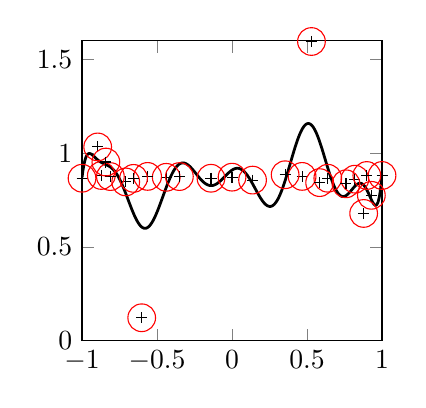
\begin{tikzpicture}

\begin{axis}[%
width=1.5in,
height=1.5in,
scale only axis,
xmin=-1,
xmax=1,
ymin=0,
ymax=1.6,
]
\addplot [color=black,solid,line width=1.0pt,forget plot]
  table[row sep=crcr]{%
-1	0.871080860495567\\
-0.993333333333333	0.911502629518509\\
-0.986666666666667	0.942155033349991\\
-0.98	0.964632302522659\\
-0.973333333333333	0.980349034070969\\
-0.966666666666667	0.990556582808495\\
-0.96	0.9963508695364\\
-0.953333333333333	0.998680248856544\\
-0.946666666666667	0.998367384076118\\
-0.94	0.996106117963791\\
-0.933333333333333	0.992481872439384\\
-0.926666666666667	0.987978920340538\\
-0.92	0.982987523078918\\
-0.913333333333333	0.977815002202988\\
-0.906666666666667	0.972697615623474\\
-0.9	0.96780252456665\\
-0.893333333333333	0.963245391845703\\
-0.886666666666667	0.959086954593658\\
-0.88	0.95534884929657\\
-0.873333333333333	0.952018141746521\\
-0.866666666666667	0.949049085378647\\
-0.86	0.946376800537109\\
-0.853333333333333	0.943917810916901\\
-0.846666666666667	0.941576242446899\\
-0.84	0.9392469227314\\
-0.833333333333333	0.93682137131691\\
-0.826666666666667	0.934192031621933\\
-0.82	0.931251436471939\\
-0.813333333333333	0.92789962887764\\
-0.806666666666667	0.9240443110466\\
-0.8	0.919603675603867\\
-0.793333333333333	0.914504885673523\\
-0.786666666666667	0.908692896366119\\
-0.78	0.902121216058731\\
-0.773333333333333	0.894760251045227\\
-0.766666666666667	0.886597096920013\\
-0.76	0.877629578113556\\
-0.753333333333333	0.867873221635818\\
-0.746666666666667	0.857357293367386\\
-0.74	0.846123650670052\\
-0.733333333333333	0.834228068590164\\
-0.726666666666667	0.821737840771675\\
-0.72	0.808730319142342\\
-0.713333333333333	0.795296087861061\\
-0.706666666666667	0.781528398394585\\
-0.7	0.767531737685204\\
-0.693333333333333	0.753416746854782\\
-0.686666666666667	0.739292293787003\\
-0.68	0.725278481841087\\
-0.673333333333333	0.711488783359528\\
-0.666666666666667	0.698043018579483\\
-0.66	0.685054257512093\\
-0.653333333333333	0.672637715935707\\
-0.646666666666667	0.660898894071579\\
-0.64	0.649943292140961\\
-0.633333333333333	0.639865696430206\\
-0.626666666666667	0.630756840109825\\
-0.62	0.622696757316589\\
-0.613333333333333	0.615755975246429\\
-0.606666666666667	0.609998196363449\\
-0.6	0.605473458766937\\
-0.593333333333333	0.60222239792347\\
-0.586666666666667	0.600273624062538\\
-0.58	0.599646255373955\\
-0.573333333333333	0.600346460938454\\
-0.566666666666667	0.602367475628853\\
-0.56	0.605694100260735\\
-0.553333333333333	0.610296815633774\\
-0.546666666666667	0.616138964891434\\
-0.54	0.623170450329781\\
-0.533333333333333	0.631334185600281\\
-0.526666666666667	0.640562996268272\\
-0.52	0.650778338313103\\
-0.513333333333333	0.661899149417877\\
-0.506666666666667	0.673834100365639\\
-0.5	0.686486691236496\\
-0.493333333333333	0.699757725000381\\
-0.486666666666667	0.713542088866234\\
-0.48	0.727729886770248\\
-0.473333333333333	0.742213517427444\\
-0.466666666666667	0.756881728768349\\
-0.46	0.771623402833939\\
-0.453333333333333	0.786330074071884\\
-0.446666666666667	0.800893738865852\\
-0.44	0.815209925174713\\
-0.433333333333333	0.829179733991623\\
-0.426666666666667	0.84270504117012\\
-0.42	0.855695381760597\\
-0.413333333333333	0.86806845664978\\
-0.406666666666667	0.879745975136757\\
-0.4	0.890659108757973\\
-0.393333333333333	0.900742694735527\\
-0.386666666666667	0.909945920109749\\
-0.38	0.918224185705185\\
-0.373333333333333	0.925541177392006\\
-0.366666666666667	0.931869179010391\\
-0.36	0.937193647027016\\
-0.353333333333333	0.941503748297691\\
-0.346666666666667	0.944800466299057\\
-0.34	0.947096586227417\\
-0.333333333333333	0.948407918214798\\
-0.326666666666667	0.948765575885773\\
-0.32	0.948200985789299\\
-0.313333333333333	0.946759149432182\\
-0.306666666666667	0.94449208676815\\
-0.3	0.941452398896217\\
-0.293333333333333	0.937706157565117\\
-0.286666666666667	0.933319866657257\\
-0.28	0.928366214036942\\
-0.273333333333333	0.922920152544975\\
-0.266666666666667	0.917060032486916\\
-0.26	0.910868540406227\\
-0.253333333333333	0.904427960515022\\
-0.246666666666667	0.897821091115475\\
-0.24	0.891130410134792\\
-0.233333333333333	0.884435974061489\\
-0.226666666666667	0.877819575369358\\
-0.22	0.871357694268227\\
-0.213333333333333	0.865123048424721\\
-0.206666666666667	0.859186753630638\\
-0.2	0.853613950312138\\
-0.193333333333333	0.848463349044323\\
-0.186666666666667	0.843789294362068\\
-0.18	0.839641496539116\\
-0.173333333333333	0.836059704422951\\
-0.166666666666667	0.833075359463692\\
-0.16	0.830720953643322\\
-0.153333333333333	0.829012244939804\\
-0.146666666666667	0.827961318194866\\
-0.14	0.827573850750923\\
-0.133333333333333	0.827842928469181\\
-0.126666666666667	0.82876156270504\\
-0.12	0.830307520925999\\
-0.113333333333333	0.832457154989243\\
-0.106666666666667	0.835175640881062\\
-0.1	0.838425040245056\\
-0.0933333333333333	0.842160582542419\\
-0.0866666666666666	0.846328571438789\\
-0.08	0.85087513178587\\
-0.0733333333333333	0.85573810338974\\
-0.0666666666666667	0.860852085053921\\
-0.0599999999999999	0.866150192916393\\
-0.0533333333333332	0.871560797095299\\
-0.0466666666666666	0.877013586461544\\
-0.0399999999999999	0.882432840764523\\
-0.0333333333333333	0.887744709849358\\
-0.0266666666666666	0.892876751720905\\
-0.0199999999999999	0.897755928337574\\
-0.0133333333333333	0.90231179445982\\
-0.0066666666666666	0.906478516757488\\
0	0.910189259797335\\
0.0066666666666666	0.913385834544897\\
0.0133333333333333	0.916010562330484\\
0.0199999999999999	0.91801467910409\\
0.0266666666666666	0.919353485107422\\
0.0333333333333333	0.919989462941885\\
0.0399999999999999	0.919890467077494\\
0.0466666666666666	0.919034343212843\\
0.0533333333333332	0.91740246117115\\
0.0599999999999999	0.914986532181501\\
0.0666666666666667	0.911790367215872\\
0.0733333333333333	0.907816376537085\\
0.08	0.90308354049921\\
0.0866666666666666	0.897616751492023\\
0.0933333333333333	0.891445942223072\\
0.1	0.884612485766411\\
0.106666666666667	0.877163052558899\\
0.113333333333333	0.869156200438738\\
0.12	0.860649693757296\\
0.126666666666667	0.85171477496624\\
0.133333333333333	0.842425398528576\\
0.14	0.832860797643661\\
0.146666666666667	0.823106683790684\\
0.153333333333333	0.813250411301851\\
0.16	0.803384441882372\\
0.166666666666667	0.793602962046862\\
0.173333333333333	0.784001410007477\\
0.18	0.774678912013769\\
0.186666666666667	0.765729982405901\\
0.193333333333333	0.757250688970089\\
0.2	0.749335628002882\\
0.206666666666667	0.74207784421742\\
0.213333333333333	0.735562892630696\\
0.22	0.729876494035125\\
0.226666666666667	0.725096607580781\\
0.233333333333333	0.721294661983848\\
0.24	0.718539644032717\\
0.246666666666667	0.716888803988695\\
0.253333333333333	0.716390825808048\\
0.26	0.717090347781777\\
0.266666666666667	0.719019865617156\\
0.273333333333333	0.722202422097325\\
0.28	0.726652130484581\\
0.286666666666667	0.732371956110001\\
0.293333333333333	0.739354087039828\\
0.3	0.747583108022809\\
0.306666666666667	0.757028132677078\\
0.313333333333333	0.76765276864171\\
0.32	0.779406264424324\\
0.326666666666667	0.792227491736412\\
0.333333333333333	0.806052768602967\\
0.34	0.820799851790071\\
0.346666666666667	0.836381698958576\\
0.353333333333333	0.852702875621617\\
0.36	0.869661035016179\\
0.366666666666667	0.887145509943366\\
0.373333333333333	0.905039585195482\\
0.38	0.923223889432847\\
0.386666666666667	0.941570690833032\\
0.393333333333333	0.959950605407357\\
0.4	0.97823385708034\\
0.406666666666667	0.996289753355086\\
0.413333333333333	1.013980303891\\
0.42	1.0311810048297\\
0.426666666666667	1.04775645956397\\
0.433333333333333	1.06358524225652\\
0.44	1.07854454126209\\
0.446666666666667	1.09251660481095\\
0.453333333333333	1.10539527703077\\
0.46	1.11707504559308\\
0.466666666666667	1.12746537663043\\
0.473333333333333	1.13647929020226\\
0.48	1.14404658041894\\
0.486666666666667	1.15010186750442\\
0.493333333333333	1.15459522744641\\
0.5	1.15748983668163\\
0.506666666666667	1.15875590825453\\
0.513333333333333	1.15838513476774\\
0.52	1.15637653833255\\
0.526666666666667	1.15274527110159\\
0.533333333333333	1.14752023573965\\
0.54	1.14074295014143\\
0.546666666666667	1.13246828131378\\
0.553333333333333	1.12276478391141\\
0.56	1.11171564180404\\
0.566666666666667	1.09941092459485\\
0.573333333333333	1.08595735626295\\
0.58	1.07146791135892\\
0.586666666666667	1.05606869980693\\
0.593333333333333	1.0398910632357\\
0.6	1.02307299943641\\
0.606666666666667	1.00576433446258\\
0.613333333333333	0.988112322287634\\
0.62	0.970271246973425\\
0.626666666666667	0.952398091787472\\
0.633333333333333	0.934646362205967\\
0.64	0.917167344130576\\
0.646666666666667	0.900116100674495\\
0.653333333333333	0.883634599624202\\
0.66	0.867865458829328\\
0.666666666666667	0.852937435498461\\
0.673333333333333	0.83897241554223\\
0.68	0.826080629369244\\
0.686666666666667	0.814359018811956\\
0.693333333333333	0.803892683237791\\
0.7	0.79474739311263\\
0.706666666666667	0.78697609109804\\
0.713333333333333	0.780612038681284\\
0.72	0.775671270559542\\
0.726666666666667	0.772151695215143\\
0.733333333333333	0.770026609883644\\
0.74	0.769256696337834\\
0.746666666666667	0.76977717585396\\
0.753333333333333	0.771506590070203\\
0.76	0.774344218429178\\
0.766666666666667	0.77817104884889\\
0.773333333333333	0.782848771777935\\
0.78	0.788225708296522\\
0.786666666666667	0.794133519404568\\
0.793333333333333	0.800392117584124\\
0.8	0.806813869741745\\
0.806666666666667	0.813201332115568\\
0.813333333333333	0.819351937971078\\
0.82	0.825063803815283\\
0.826666666666667	0.830138723133132\\
0.833333333333333	0.83437842753483\\
0.84	0.837607907014899\\
0.846666666666667	0.839651910820976\\
0.853333333333333	0.840369191719219\\
0.86	0.839634875650518\\
0.866666666666667	0.837361696409062\\
0.873333333333333	0.833497695683036\\
0.88	0.828032078105025\\
0.886666666666667	0.821004733617883\\
0.893333333333333	0.812513404875062\\
0.9	0.802719077037182\\
0.906666666666667	0.791851329617202\\
0.913333333333333	0.780216799757909\\
0.92	0.76820944721112\\
0.926666666666667	0.756314025842585\\
0.933333333333333	0.745112903183326\\
0.94	0.735300561675103\\
0.946666666666667	0.727681809483329\\
0.953333333333333	0.723186431045178\\
0.96	0.722874706989387\\
0.966666666666667	0.727942201192491\\
0.973333333333333	0.739730050147045\\
0.98	0.759731092053698\\
0.986666666666667	0.789598370873136\\
0.993333333333333	0.831147338292794\\
1	0.886367861414328\\
};
\addplot [color=black,only marks,mark=+,mark options={solid},forget plot]
  table[row sep=crcr]{%
0.818827708703375	0.861888122983872\\
};
\addplot [color=red,mark size=5.0pt,only marks,mark=o,mark options={solid},forget plot]
  table[row sep=crcr]{%
0.818827708703375	0.861888122983872\\
};
\addplot [color=black,only marks,mark=+,mark options={solid},forget plot]
  table[row sep=crcr]{%
0.136767317939609	0.856960457661291\\
};
\addplot [color=red,mark size=5.0pt,only marks,mark=o,mark options={solid},forget plot]
  table[row sep=crcr]{%
0.136767317939609	0.856960457661291\\
};
\addplot [color=black,only marks,mark=+,mark options={solid},forget plot]
  table[row sep=crcr]{%
-0.438721136767318	0.871743453629032\\
};
\addplot [color=red,mark size=5.0pt,only marks,mark=o,mark options={solid},forget plot]
  table[row sep=crcr]{%
-0.438721136767318	0.871743453629032\\
};
\addplot [color=black,only marks,mark=+,mark options={solid},forget plot]
  table[row sep=crcr]{%
-1	0.866815788306452\\
};
\addplot [color=red,mark size=5.0pt,only marks,mark=o,mark options={solid},forget plot]
  table[row sep=crcr]{%
-1	0.866815788306452\\
};
\addplot [color=black,only marks,mark=+,mark options={solid},forget plot]
  table[row sep=crcr]{%
-0.708703374777975	0.847105127016129\\
};
\addplot [color=red,mark size=5.0pt,only marks,mark=o,mark options={solid},forget plot]
  table[row sep=crcr]{%
-0.708703374777975	0.847105127016129\\
};
\addplot [color=black,only marks,mark=+,mark options={solid},forget plot]
  table[row sep=crcr]{%
-0.140319715808171	0.866815788306452\\
};
\addplot [color=red,mark size=5.0pt,only marks,mark=o,mark options={solid},forget plot]
  table[row sep=crcr]{%
-0.140319715808171	0.866815788306452\\
};
\addplot [color=black,only marks,mark=+,mark options={solid},forget plot]
  table[row sep=crcr]{%
0.467140319715808	0.876671118951613\\
};
\addplot [color=red,mark size=5.0pt,only marks,mark=o,mark options={solid},forget plot]
  table[row sep=crcr]{%
0.467140319715808	0.876671118951613\\
};
\addplot [color=black,only marks,mark=+,mark options={solid},forget plot]
  table[row sep=crcr]{%
1	0.881598784274194\\
};
\addplot [color=red,mark size=5.0pt,only marks,mark=o,mark options={solid},forget plot]
  table[row sep=crcr]{%
1	0.881598784274194\\
};
\addplot [color=black,only marks,mark=+,mark options={solid},forget plot]
  table[row sep=crcr]{%
0.529500756429652	1.59611025604839\\
};
\addplot [color=red,mark size=5.0pt,only marks,mark=o,mark options={solid},forget plot]
  table[row sep=crcr]{%
0.529500756429652	1.59611025604839\\
};
\addplot [color=black,only marks,mark=+,mark options={solid},forget plot]
  table[row sep=crcr]{%
-0.602118003025719	0.122738324596774\\
};
\addplot [color=red,mark size=5.0pt,only marks,mark=o,mark options={solid},forget plot]
  table[row sep=crcr]{%
-0.602118003025719	0.122738324596774\\
};
\addplot [color=black,only marks,mark=+,mark options={solid},forget plot]
  table[row sep=crcr]{%
0.638426626323752	0.866815788306452\\
};
\addplot [color=red,mark size=5.0pt,only marks,mark=o,mark options={solid},forget plot]
  table[row sep=crcr]{%
0.638426626323752	0.866815788306452\\
};
\addplot [color=black,only marks,mark=+,mark options={solid},forget plot]
  table[row sep=crcr]{%
-0.871406959152799	0.881598784274194\\
};
\addplot [color=red,mark size=5.0pt,only marks,mark=o,mark options={solid},forget plot]
  table[row sep=crcr]{%
-0.871406959152799	0.881598784274194\\
};
\addplot [color=black,only marks,mark=+,mark options={solid},forget plot]
  table[row sep=crcr]{%
-0.562783661119516	0.876671118951613\\
};
\addplot [color=red,mark size=5.0pt,only marks,mark=o,mark options={solid},forget plot]
  table[row sep=crcr]{%
-0.562783661119516	0.876671118951613\\
};
\addplot [color=black,only marks,mark=+,mark options={solid},forget plot]
  table[row sep=crcr]{%
0.898638426626323	0.881598784274194\\
};
\addplot [color=red,mark size=5.0pt,only marks,mark=o,mark options={solid},forget plot]
  table[row sep=crcr]{%
0.898638426626323	0.881598784274194\\
};
\addplot [color=black,only marks,mark=+,mark options={solid},forget plot]
  table[row sep=crcr]{%
0.75945537065053	0.837096774193548\\
};
\addplot [color=red,mark size=5.0pt,only marks,mark=o,mark options={solid},forget plot]
  table[row sep=crcr]{%
0.75945537065053	0.837096774193548\\
};
\addplot [color=black,only marks,mark=+,mark options={solid},forget plot]
  table[row sep=crcr]{%
-0.81089258698941	0.875806451612903\\
};
\addplot [color=red,mark size=5.0pt,only marks,mark=o,mark options={solid},forget plot]
  table[row sep=crcr]{%
-0.81089258698941	0.875806451612903\\
};
\addplot [color=black,only marks,mark=+,mark options={solid},forget plot]
  table[row sep=crcr]{%
0.583963691376702	0.843548387096774\\
};
\addplot [color=red,mark size=5.0pt,only marks,mark=o,mark options={solid},forget plot]
  table[row sep=crcr]{%
0.583963691376702	0.843548387096774\\
};
\addplot [color=black,only marks,mark=+,mark options={solid},forget plot]
  table[row sep=crcr]{%
-0.656580937972769	0.866129032258065\\
};
\addplot [color=red,mark size=5.0pt,only marks,mark=o,mark options={solid},forget plot]
  table[row sep=crcr]{%
-0.656580937972769	0.866129032258065\\
};
\addplot [color=black,only marks,mark=+,mark options={solid},forget plot]
  table[row sep=crcr]{%
-0.350983358547655	0.875806451612903\\
};
\addplot [color=red,mark size=5.0pt,only marks,mark=o,mark options={solid},forget plot]
  table[row sep=crcr]{%
-0.350983358547655	0.875806451612903\\
};
\addplot [color=black,only marks,mark=+,mark options={solid},forget plot]
  table[row sep=crcr]{%
0	0.87258064516129\\
};
\addplot [color=red,mark size=5.0pt,only marks,mark=o,mark options={solid},forget plot]
  table[row sep=crcr]{%
0	0.87258064516129\\
};
\addplot [color=black,only marks,mark=+,mark options={solid},forget plot]
  table[row sep=crcr]{%
0.354009077155824	0.885483870967742\\
};
\addplot [color=red,mark size=5.0pt,only marks,mark=o,mark options={solid},forget plot]
  table[row sep=crcr]{%
0.354009077155824	0.885483870967742\\
};
\addplot [color=black,only marks,mark=+,mark options={solid},forget plot]
  table[row sep=crcr]{%
0.877458396369138	0.679032258064516\\
};
\addplot [color=red,mark size=5.0pt,only marks,mark=o,mark options={solid},forget plot]
  table[row sep=crcr]{%
0.877458396369138	0.679032258064516\\
};
\addplot [color=black,only marks,mark=+,mark options={solid},forget plot]
  table[row sep=crcr]{%
-0.895612708018154	1.03387096774194\\
};
\addplot [color=red,mark size=5.0pt,only marks,mark=o,mark options={solid},forget plot]
  table[row sep=crcr]{%
-0.895612708018154	1.03387096774194\\
};
\addplot [color=black,only marks,mark=+,mark options={solid},forget plot]
  table[row sep=crcr]{%
0.928895612708018	0.775806451612903\\
};
\addplot [color=red,mark size=5.0pt,only marks,mark=o,mark options={solid},forget plot]
  table[row sep=crcr]{%
0.928895612708018	0.775806451612903\\
};
\addplot [color=black,only marks,mark=+,mark options={solid},forget plot]
  table[row sep=crcr]{%
-0.841149773071104	0.953225806451613\\
};
\addplot [color=red,mark size=5.0pt,only marks,mark=o,mark options={solid},forget plot]
  table[row sep=crcr]{%
-0.841149773071104	0.953225806451613\\
};
\end{axis}
\end{tikzpicture}%
\end{document}
\caption{On this data set the linear kernel is able to outperform a radial basis function kernel, which is more susceptible to the noisy outliers.}
\label{fig:linearKing}
\end{figure}
Figure~\ref{fig:linearKing} shows an example of an approximately line-like function with some outliers. In this case a simple linear kernel is a good choice, as it is unable to track the added complexity of the noise. An rbf-function kernel is able to integrate the noise into the model, but in this example one would like to avoid this. However it is possible to fundamentally improve the rbf kernel results if changes the parameters $\sigma, c$ and $\epsilon$ are changed more towards regularization. Most notably the parameter $c$, which determines the tolerance for deviation from the desired $\epsilon$-accuracy can be used to improve the performance of the rbf-kernel. If $c$ is set to a comparatively large value with $\epsilon$ kept small results improve. A good choice will use a moderate value for $\epsilon$ to reduce the amount of support vectors and thereby increases the sparsity of the solution vector\footnote{Support Vector Machines: Methods and Applications, Suykens et al., page 33}, while using $c$ to make sure the solution is not to prone to deviations introduced by outliers.
 
\subsection{Sum of cosines}
As an initial example noise free function:
\begin{equation}
f(x) = \cos(x) + \cos(2x)
\end{equation}
will be considered. Finding a good set of hyper-parameters by hand can be tricky as figure~\ref{fig:estParamsTricky} illustrates. To make a good choice a hundred by hundred grid in $\sigma^2 \in [10^{-5},10^{0}]$ and $\gamma \in [10^{0},10^{10}]$  has been searched using the two norm of the error vector $(\mathbf{y}_{est} - \mathbf{y})$ as cost function. The error function on the described input space as well as the estimator with the lowest error is shown in figure~\ref{fig:cosEst}. The grid search led to optimal the parameter pair $\sigma^2 = 0.0019$ and $\gamma = 10.2353$. Estimation results are shown in the middle of figure~\ref{fig:cosEst} training set performance is plotted on the left.
Next a noisy version of $f(x)$ is considered:
\begin{equation}
f(x)_n = \cos(x) + \cos(2x) + x_n
\end{equation}
With the values for $x_n$ drawn from the normal distribution $\mathcal{N}(0,0.1^2)$. The changed situation is shown in figure~\ref{fig:cosEstNoise}. When noise is added on average the optimal values for $\sigma^2$ must be chosen larger to avoid 
over-fitting.

\begin{figure}
\centering
% This file was created by matlab2tikz.
% Minimal pgfplots version: 1.3
%
%The latest updates can be retrieved from
%  http://www.mathworks.com/matlabcentral/fileexchange/22022-matlab2tikz
%where you can also make suggestions and rate matlab2tikz.
%
\documentclass[tikz]{standalone}
\usepackage{pgfplots}
\usepackage{grffile}
\pgfplotsset{compat=newest}
\usetikzlibrary{plotmarks}
\usepackage{amsmath}

\begin{document}
\definecolor{mycolor1}{rgb}{0.00000,0.44700,0.74100}%
\definecolor{mycolor2}{rgb}{0.85000,0.32500,0.09800}%
\definecolor{mycolor3}{rgb}{0.92900,0.69400,0.12500}%
\definecolor{mycolor4}{rgb}{0.49400,0.18400,0.55600}%
\definecolor{mycolor5}{rgb}{0.46600,0.67400,0.18800}%
\definecolor{mycolor6}{rgb}{0.30100,0.74500,0.93300}%
%
\begin{tikzpicture}

\begin{axis}[%
width=4.5in,
height=1.5in,
scale only axis,
xmin=-10,
xmax=10,
ymin=-1.5,
ymax=2.5
]
\addplot [color=mycolor1,solid,forget plot]
  table[row sep=crcr]{%
-10	-0.281314540932569\\
-9.99	-0.281514963345573\\
-9.98	-0.281312785960784\\
-9.97	-0.280712312116697\\
-9.96	-0.279719972322067\\
-9.95	-0.278344290785733\\
-9.94	-0.276595834672387\\
-9.93	-0.274487146397842\\
-9.92	-0.272032659456664\\
-9.91	-0.269248598451292\\
-9.9	-0.266152864161493\\
-9.89	-0.262764904656628\\
-9.88	-0.2591055736026\\
-9.87	-0.255196977058975\\
-9.86	-0.251062310185644\\
-9.85	-0.246725685391245\\
-9.84	-0.24221195355025\\
-9.83	-0.237546519991719\\
-9.82	-0.232755157022512\\
-9.81	-0.22786381478573\\
-9.8	-0.222898432273032\\
-9.79	-0.217884750309779\\
-9.78	-0.21284812830903\\
-9.77	-0.207813366546944\\
-9.76	-0.20280453565507\\
-9.75	-0.197844814937499\\
-9.74	-0.192956341029585\\
-9.73	-0.188160068293018\\
-9.72	-0.183475642214507\\
-9.71	-0.178921286929833\\
-9.7	-0.174513707835273\\
-9.69	-0.170268010082537\\
-9.68	-0.166197633575948\\
-9.67	-0.162314304907495\\
-9.66	-0.15862800647759\\
-9.65	-0.155146962861875\\
-9.64	-0.151877644293432\\
-9.63	-0.148824786943972\\
-9.62	-0.145991429507214\\
-9.61	-0.143378965410722\\
-9.6	-0.14098720981927\\
-9.59	-0.138814480435887\\
-9.58	-0.136857690968655\\
-9.57	-0.135112456000846\\
-9.56	-0.133573205895139\\
-9.55	-0.132233310266855\\
-9.54	-0.131085208489584\\
-9.53	-0.130120545639723\\
-9.52	-0.129330312253576\\
-9.51	-0.128704986255606\\
-9.5	-0.128234675423641\\
-9.49	-0.127909258782426\\
-9.48	-0.127718525364703\\
-9.47	-0.127652308843286\\
-9.46	-0.127700616620711\\
-9.45	-0.127853752063886\\
-9.44	-0.128102428684805\\
-9.43	-0.128437875197141\\
-9.42	-0.128851930517542\\
-9.41	-0.129337127929298\\
-9.4	-0.129886767781683\\
-9.39	-0.130494978258281\\
-9.38	-0.131156763911118\\
-9.37	-0.131868041818931\\
-9.36	-0.132625665389351\\
-9.35	-0.133427435980262\\
-9.34	-0.134272102663186\\
-9.33	-0.135159350594363\\
-9.32	-0.136089778585651\\
-9.31	-0.137064866585421\\
-9.3	-0.138086933884269\\
-9.29	-0.13915908894532\\
-9.28	-0.140285171834718\\
-9.27	-0.141469690279986\\
-9.26	-0.142717750426185\\
-9.25	-0.144034983378473\\
-9.24	-0.145427468627122\\
-9.23	-0.14690165543898\\
-9.22	-0.148464283272134\\
-9.21	-0.150122302231171\\
-9.2	-0.151882794525531\\
-9.19	-0.153752897826963\\
-9.18	-0.155739731347624\\
-9.17	-0.157850325375415\\
-9.16	-0.160091554911523\\
-9.15	-0.162470077960965\\
-9.14	-0.164992278928175\\
-9.13	-0.167664217469019\\
-9.12	-0.170491583054297\\
-9.11	-0.173479655402364\\
-9.1	-0.176633270847273\\
-9.09	-0.179956794622555\\
-9.08	-0.183454098961386\\
-9.07	-0.187128546842724\\
-9.06	-0.19098298114927\\
-9.05	-0.195019718950958\\
-9.04	-0.199240550582902\\
-9.03	-0.203646743152962\\
-9.02	-0.208239048090579\\
-9.01	-0.213017712333237\\
-9	-0.217982492741302\\
-8.99	-0.223132673335565\\
-8.98	-0.22846708496061\\
-8.97	-0.233984126995501\\
-8.96	-0.239681790754383\\
-8.95	-0.245557684246793\\
-8.94	-0.251609057997815\\
-8.93	-0.257832831658442\\
-8.92	-0.264225621171866\\
-8.91	-0.270783766290651\\
-8.9	-0.277503358273526\\
-8.89	-0.284380267618095\\
-8.88	-0.291410171709968\\
-8.87	-0.298588582294157\\
-8.86	-0.305910872687579\\
-8.85	-0.313372304667875\\
-8.84	-0.320968054978654\\
-8.83	-0.32869324139594\\
-8.82	-0.336542948296551\\
-8.81	-0.344512251664149\\
-8.8	-0.352596243457\\
-8.79	-0.360790055245653\\
-8.78	-0.36908888101529\\
-8.77	-0.3774879990028\\
-8.76	-0.385982792424163\\
-8.75	-0.394568768921073\\
-8.74	-0.403241578541732\\
-8.73	-0.41199703004568\\
-8.72	-0.420831105314727\\
-8.71	-0.429739971630995\\
-8.7	-0.438719991583566\\
-8.69	-0.447767730355128\\
-8.68	-0.456879960147055\\
-8.67	-0.466053661507391\\
-8.66	-0.475286021342631\\
-8.65	-0.484574427413347\\
-8.64	-0.49391645914403\\
-8.63	-0.503309874609057\\
-8.62	-0.512752593598883\\
-8.61	-0.522242676713917\\
-8.6	-0.531778300486991\\
-8.59	-0.541357728586389\\
-8.58	-0.550979279213143\\
-8.57	-0.560641288862703\\
-8.56	-0.570342072687978\\
-8.55	-0.580079881755022\\
-8.54	-0.589852857552549\\
-8.53	-0.599658984166897\\
-8.52	-0.609496038595417\\
-8.51	-0.61936153971896\\
-8.5	-0.629252696502169\\
-8.49	-0.639166356027477\\
-8.48	-0.64909895200175\\
-8.47	-0.659046454399172\\
-8.46	-0.669004320916868\\
-8.45	-0.67896745092842\\
-8.44	-0.688930142612978\\
-8.43	-0.698886053928962\\
-8.42	-0.708828168073238\\
-8.41	-0.718748764035016\\
-8.4	-0.728639392814604\\
-8.39	-0.738490859816404\\
-8.38	-0.748293213877337\\
-8.37	-0.758035743312854\\
-8.36	-0.767706979294461\\
-8.35	-0.777294706789622\\
-8.34	-0.786785983209126\\
-8.33	-0.796167164817734\\
-8.32	-0.805423940872025\\
-8.31	-0.814541375354869\\
-8.3	-0.823503956085401\\
-8.29	-0.832295650886574\\
-8.28	-0.840899970408256\\
-8.27	-0.849300037112269\\
-8.26	-0.857478659851089\\
-8.25	-0.865418413390653\\
-8.24	-0.87310172216653\\
-8.23	-0.880510947496865\\
-8.22	-0.887628477432233\\
-8.21	-0.894436818375163\\
-8.2	-0.900918687576228\\
-8.19	-0.907057105592265\\
-8.18	-0.912835487785392\\
-8.17	-0.918237733942317\\
-8.16	-0.923248315111488\\
-8.15	-0.927852356777898\\
-8.14	-0.932035717535055\\
-8.13	-0.935785062459456\\
-8.12	-0.939087930452624\\
-8.11	-0.941932794879106\\
-8.1	-0.944309116909194\\
-8.09	-0.946207391054955\\
-8.08	-0.947619182478503\\
-8.07	-0.948537155747513\\
-8.06	-0.948955094812854\\
-8.05	-0.948867914081857\\
-8.04	-0.948271660570243\\
-8.03	-0.947163507212938\\
-8.02	-0.945541737523398\\
-8.01	-0.943405721884041\\
-8	-0.940755885852049\\
-7.99	-0.937593670951805\\
-7.98	-0.933921488510176\\
-7.97	-0.929742667165982\\
-7.96	-0.925061394755145\\
-7.95	-0.919882655324897\\
-7.94	-0.91421216208403\\
-7.93	-0.908056287124502\\
-7.92	-0.901421988780443\\
-7.91	-0.894316737496068\\
-7.9	-0.886748441078347\\
-7.89	-0.878725370193867\\
-7.88	-0.870256084947569\\
-7.87	-0.86134936334294\\
-7.86	-0.852014132377324\\
-7.85	-0.842259402469203\\
-7.84	-0.832094205845757\\
-7.83	-0.821527539449023\\
-7.82	-0.810568312833133\\
-7.81	-0.799225301441638\\
-7.8	-0.787507105562497\\
-7.79	-0.775422115164543\\
-7.78	-0.762978480725116\\
-7.77	-0.750184090065739\\
-7.76	-0.737046551119681\\
-7.75	-0.723573180467586\\
-7.74	-0.709770997395478\\
-7.73	-0.695646723150377\\
-7.72	-0.68120678500114\\
-7.71	-0.666457324651573\\
-7.7	-0.651404210500774\\
-7.69	-0.636053053205922\\
-7.68	-0.620409223972816\\
-7.67	-0.604477874980455\\
-7.66	-0.588263961339533\\
-7.65	-0.571772263988078\\
-7.64	-0.555007412944064\\
-7.63	-0.537973910360081\\
-7.62	-0.520676152861217\\
-7.61	-0.503118452692647\\
-7.6	-0.485305057257609\\
-7.59	-0.467240166686225\\
-7.58	-0.448927949141973\\
-7.57	-0.430372553644808\\
-7.56	-0.411578120261673\\
-7.55	-0.392548787593278\\
-7.54	-0.373288697559621\\
-7.53	-0.353801997562412\\
-7.52	-0.334092840173472\\
-7.51	-0.314165380566233\\
-7.5	-0.294023771968495\\
-7.49	-0.273672159471775\\
-7.48	-0.253114672578441\\
-7.47	-0.2323554169094\\
-7.46	-0.211398465523416\\
-7.45	-0.190247850321002\\
-7.44	-0.168907554015679\\
-7.43	-0.147381503156238\\
-7.42	-0.125673562671971\\
-7.41	-0.103787532395554\\
-7.4	-0.081727145985703\\
-7.39	-0.0594960726354438\\
-7.38	-0.0370979219024517\\
-7.37	-0.014536251945899\\
-7.36	0.00818541860952005\\
-7.35	0.0310635950262849\\
-7.34	0.0540947869395819\\
-7.33	0.0772754849642756\\
-7.32	0.100602133489423\\
-7.31	0.124071099800748\\
-7.3	0.147678639747935\\
-7.29	0.171420860246294\\
-7.28	0.195293678972361\\
-7.27	0.219292781677734\\
-7.26	0.243413577606523\\
-7.25	0.267651153552968\\
-7.24	0.292000227143247\\
-7.23	0.316455099961497\\
-7.22	0.341009611169387\\
-7.21	0.365657092287297\\
-7.2	0.390390323814951\\
-7.19	0.415201494368224\\
-7.18	0.440082162999537\\
-7.17	0.465023225347215\\
-7.16	0.490014884231525\\
-7.15	0.515046625273302\\
-7.14	0.540107198065992\\
-7.13	0.565184603372934\\
-7.12	0.590266086761479\\
-7.11	0.615338139012603\\
-7.1	0.640386503572531\\
-7.09	0.665396191228827\\
-7.08	0.690351502115142\\
-7.07	0.71523605505707\\
-7.06	0.74003282419111\\
-7.05	0.764724182695079\\
-7.04	0.789291953389035\\
-7.03	0.813717465876064\\
-7.02	0.83798161981788\\
-7.01	0.862064953860476\\
-7	0.885947719657401\\
-6.99	0.909609960374326\\
-6.98	0.933031593002477\\
-6.97	0.956192493759894\\
-6.96	0.979072585822421\\
-6.95	1.00165192859446\\
-6.94	1.02391080771015\\
-6.93	1.04582982494701\\
-6.92	1.06738998723202\\
-6.91	1.08857279393298\\
-6.9	1.10936032164508\\
-6.89	1.129735305717\\
-6.88	1.14968121779428\\
-6.87	1.1691823387131\\
-6.86	1.18822382612574\\
-6.85	1.20679177630779\\
-6.84	1.22487327966438\\
-6.83	1.24245646952676\\
-6.82	1.25953056391095\\
-6.81	1.2760858999901\\
-6.8	1.29211396111709\\
-6.79	1.30760739631739\\
-6.78	1.32256003225648\\
-6.77	1.3369668777651\\
-6.76	1.35082412108912\\
-6.75	1.36412912009894\\
-6.74	1.37688038576846\\
-6.73	1.38907755929277\\
-6.72	1.40072138327115\\
-6.71	1.41181366743089\\
-6.7	1.42235724940616\\
-6.69	1.43235595111837\\
-6.68	1.44181453132712\\
-6.67	1.45073863493157\\
-6.66	1.45913473961042\\
-6.65	1.46701010037799\\
-6.64	1.47437269262552\\
-6.63	1.48123115419184\\
-6.62	1.48759472698007\\
-6.61	1.49347319859947\\
-6.6	1.49887684447215\\
-6.59	1.503816370794\\
-6.58	1.50830285869428\\
-6.57	1.51234770987897\\
-6.56	1.51596259399186\\
-6.55	1.51915939787049\\
-6.54	1.52195017682036\\
-6.53	1.52434710797621\\
-6.52	1.52636244576968\\
-6.51	1.52800847947626\\
-6.5	1.52929749277103\\
-6.49	1.53024172518802\\
-6.48	1.53085333534571\\
-6.47	1.53114436577686\\
-6.46	1.53112670918534\\
-6.45	1.53081207593989\\
-6.44	1.53021196261406\\
-6.43	1.5293376213836\\
-6.42	1.52820003010529\\
-6.41	1.52680986291739\\
-6.4	1.52517746122477\\
-6.39	1.52331280496319\\
-6.38	1.52122548406772\\
-6.37	1.51892467010896\\
-6.36	1.51641908810097\\
-6.35	1.51371698852689\\
-6.34	1.51082611967142\\
-6.33	1.5077537003922\\
-6.32	1.50450639350565\\
-6.31	1.50109027999985\\
-6.3	1.49751083433072\\
-6.29	1.49377290108148\\
-6.28	1.48988067330471\\
-6.27	1.48583767288221\\
-6.26	1.48164673325779\\
-6.25	1.47730998491015\\
-6.24	1.47282884393468\\
-6.23	1.46820400410295\\
-6.22	1.46343543275331\\
-6.21	1.45852237085393\\
-6.2	1.45346333754922\\
-6.19	1.44825613947191\\
-6.18	1.44289788506287\\
-6.17	1.43738500409565\\
-6.16	1.43171327255221\\
-6.15	1.42587784294068\\
-6.14	1.41987328008836\\
-6.13	1.41369360237578\\
-6.12	1.40733232831487\\
-6.11	1.40078252830907\\
-6.1	1.39403688136068\\
-6.09	1.3870877364269\\
-6.08	1.37992717805974\\
-6.07	1.37254709589979\\
-6.06	1.36493925753344\\
-6.05	1.35709538417038\\
-6.04	1.34900722854113\\
-6.03	1.34066665437154\\
-6.02	1.33206571675534\\
-6.01	1.3231967427063\\
-6	1.3140524111539\\
-5.99	1.30462583162648\\
-5.98	1.29491062086009\\
-5.97	1.28490097656797\\
-5.96	1.27459174762166\\
-5.95	1.26397849990781\\
-5.94	1.2530575771523\\
-5.93	1.24182615604537\\
-5.92	1.23028229503566\\
-5.91	1.21842497622218\\
-5.9	1.20625413982814\\
-5.89	1.19377071080794\\
-5.88	1.18097661721189\\
-5.87	1.16787480001057\\
-5.86	1.15446921416393\\
-5.85	1.1407648208061\\
-5.84	1.12676757050811\\
-5.83	1.11248437766752\\
-5.82	1.09792308617118\\
-5.81	1.08309242656454\\
-5.8	1.06800196505408\\
-5.79	1.05266204475504\\
-5.78	1.03708371968461\\
-5.77	1.02127868207688\\
-5.76	1.0052591836742\\
-5.75	0.989037951717485\\
-5.74	0.972628100418822\\
-5.73	0.956043038754482\\
-5.72	0.939296375461636\\
-5.71	0.922401822159938\\
-5.7	0.905373095541684\\
-5.69	0.888223819596886\\
-5.68	0.87096742884108\\
-5.67	0.853617073513083\\
-5.66	0.836185527693535\\
-5.65	0.818685101272714\\
-5.64	0.801127556658907\\
-5.63	0.783524031076072\\
-5.62	0.765884965244753\\
-5.61	0.748220039177383\\
-5.6	0.730538115748937\\
-5.59	0.712847192624678\\
-5.58	0.695154363042676\\
-5.57	0.677465785857362\\
-5.56	0.659786665156061\\
-5.55	0.642121239660755\\
-5.54	0.624472782025538\\
-5.53	0.606843608038456\\
-5.52	0.58923509563115\\
-5.51	0.571647713498395\\
-5.5	0.554081059028767\\
-5.49	0.5365339051479\\
-5.48	0.51900425558532\\
-5.47	0.501489407983197\\
-5.46	0.483986024185902\\
-5.45	0.466490206970957\\
-5.44	0.448997582415065\\
-5.43	0.431503387029309\\
-5.42	0.414002558746177\\
-5.41	0.396489830801186\\
-5.4	0.378959827521022\\
-5.39	0.361407161009626\\
-5.38	0.34382652771445\\
-5.37	0.326212803856716\\
-5.36	0.308561138721663\\
-5.35	0.290867044827572\\
-5.34	0.27312648402618\\
-5.33	0.255335948631243\\
-5.32	0.237492536724132\\
-5.31	0.219594020849614\\
-5.3	0.201638909384987\\
-5.29	0.183626499944995\\
-5.28	0.165556924270749\\
-5.27	0.147431184142892\\
-5.26	0.129251177955468\\
-5.25	0.111019717688646\\
-5.24	0.0927405361210486\\
-5.23	0.0744182842287807\\
-5.22	0.05605851882372\\
-5.21	0.0376676805885767\\
-5.2	0.0192530627709896\\
-5.19	0.000822770898105968\\
-5.18	-0.017614326029123\\
-5.17	-0.0360486523118261\\
-5.16	-0.0544699896637891\\
-5.15	-0.0728675479427999\\
-5.14	-0.0912300417191619\\
-5.13	-0.10954577183545\\
-5.12	-0.127802711060652\\
-5.11	-0.145988592899063\\
-5.1	-0.164091002583435\\
-5.09	-0.182097469260622\\
-5.08	-0.199995558368886\\
-5.07	-0.217772963207346\\
-5.06	-0.235417594709854\\
-5.05	-0.252917668460067\\
-5.04	-0.270261788016724\\
-5.03	-0.287439023663399\\
-5.02	-0.304438985748869\\
-5.01	-0.321251891847398\\
-5	-0.337868627037696\\
-4.99	-0.354280796676384\\
-4.98	-0.370480771126056\\
-4.97	-0.386461721985632\\
-4.96	-0.402217649464498\\
-4.95	-0.417743400637209\\
-4.94	-0.433034678413902\\
-4.93	-0.448088041160227\\
-4.92	-0.462900892999271\\
-4.91	-0.477471464925495\\
-4.9	-0.491798786955484\\
-4.89	-0.505882651632447\\
-4.88	-0.519723569288921\\
-4.87	-0.533322715554573\\
-4.86	-0.546681871672822\\
-4.85	-0.559803358260143\\
-4.84	-0.572689963205215\\
-4.83	-0.58534486446044\\
-4.82	-0.597771548525402\\
-4.81	-0.609973725462068\\
-4.8	-0.621955241310853\\
-4.79	-0.633719988799497\\
-4.78	-0.645271817249603\\
-4.77	-0.656614442590529\\
-4.76	-0.667751358386293\\
-4.75	-0.678685748769202\\
-4.74	-0.689420404154019\\
-4.73	-0.69995764057853\\
-4.72	-0.710299223481894\\
-4.71	-0.720446296690093\\
-4.7	-0.730399317330695\\
-4.69	-0.740157997344513\\
-4.68	-0.749721252204029\\
-4.67	-0.759087157384419\\
-4.66	-0.768252913065506\\
-4.65	-0.777214817472567\\
-4.64	-0.785968249190068\\
-4.63	-0.794507658705571\\
-4.62	-0.802826569365026\\
-4.61	-0.81091758783994\\
-4.6	-0.818772424128871\\
-4.59	-0.82638192103619\\
-4.58	-0.83373609299137\\
-4.57	-0.840824173995492\\
-4.56	-0.847634674404737\\
-4.55	-0.854155446186696\\
-4.54	-0.860373756213914\\
-4.53	-0.866276367090639\\
-4.52	-0.871849624943159\\
-4.51	-0.877079553544174\\
-4.5	-0.881951954082839\\
-4.49	-0.886452509842699\\
-4.48	-0.890566894999695\\
-4.47	-0.894280886713917\\
-4.46	-0.897580479650827\\
-4.45	-0.900452002039328\\
-4.44	-0.902882232350713\\
-4.43	-0.904858515665931\\
-4.42	-0.906368878790045\\
-4.41	-0.907402143169391\\
-4.4	-0.907948034672817\\
-4.39	-0.907997289311249\\
-4.38	-0.907541753989039\\
-4.37	-0.906574481408766\\
-4.36	-0.90508981828697\\
-4.35	-0.903083486079009\\
-4.34	-0.900552653463604\\
-4.33	-0.897495999891985\\
-4.32	-0.893913769572355\\
-4.31	-0.889807815328491\\
-4.3	-0.885181631848237\\
-4.29	-0.880040377918625\\
-4.28	-0.874390887329683\\
-4.27	-0.868241668220295\\
-4.26	-0.861602890731572\\
-4.25	-0.854486362930464\\
-4.24	-0.84690549506358\\
-4.23	-0.838875252299924\\
-4.22	-0.830412096220529\\
-4.21	-0.821533915409905\\
-4.2	-0.812259945600741\\
-4.19	-0.802610679915701\\
-4.18	-0.792607769838984\\
-4.17	-0.782273917635043\\
-4.16	-0.771632761009509\\
-4.15	-0.760708750879298\\
-4.14	-0.749527023183232\\
-4.13	-0.738113265720263\\
-4.12	-0.726493581049817\\
-4.11	-0.714694346526213\\
-4.1	-0.702742072567037\\
-4.09	-0.690663260272802\\
-4.08	-0.678484259522014\\
-4.07	-0.6662311286624\\
-4.06	-0.653929496904211\\
-4.05	-0.641604430496697\\
-4.04	-0.629280303733667\\
-4.03	-0.616980675788502\\
-4.02	-0.60472817432441\\
-4.01	-0.592544386761944\\
-4	-0.580449760013983\\
-3.99	-0.568463509418841\\
-3.98	-0.556603537516835\\
-3.97	-0.54488636322333\\
-3.96	-0.533327061856288\\
-3.95	-0.521939216375478\\
-3.94	-0.510734880089614\\
-3.93	-0.499724550983112\\
-3.92	-0.48891715771106\\
-3.91	-0.478320057207735\\
-3.9	-0.467939043752857\\
-3.89	-0.45777836924154\\
-3.88	-0.447840774309594\\
-3.87	-0.438127529876156\\
-3.86	-0.428638488581711\\
-3.85	-0.41937214552196\\
-3.84	-0.410325707607551\\
-3.83	-0.401495170816868\\
-3.82	-0.392875404554278\\
-3.81	-0.384460242280295\\
-3.8	-0.376242577542709\\
-3.79	-0.368214464509434\\
-3.78	-0.360367222084683\\
-3.77	-0.352691540679998\\
-3.76	-0.345177590710408\\
-3.75	-0.337815131893749\\
-3.74	-0.330593622447114\\
-3.73	-0.323502327298662\\
-3.72	-0.316530424464782\\
-3.71	-0.309667108781521\\
-3.7	-0.302901692224618\\
-3.69	-0.296223700103895\\
-3.68	-0.2896229624744\\
-3.67	-0.283089700167608\\
-3.66	-0.2766146049112\\
-3.65	-0.270188913073651\\
-3.64	-0.263804472640184\\
-3.63	-0.257453803098296\\
-3.62	-0.251130147983695\\
-3.61	-0.244827519909572\\
-3.6	-0.238540737974423\\
-3.59	-0.232265457513386\\
-3.58	-0.225998192226677\\
-3.57	-0.219736328784061\\
-3.56	-0.213478134066667\\
-3.55	-0.207222755265826\\
-3.54	-0.20097021311285\\
-3.53	-0.194721388563404\\
-3.52	-0.188478003304348\\
-3.51	-0.182242594490633\\
-3.5	-0.176018484153185\\
-3.49	-0.169809743747329\\
-3.48	-0.163621154333396\\
-3.47	-0.157458162898203\\
-3.46	-0.15132683533689\\
-3.45	-0.14523380662045\\
-3.44	-0.139186228674186\\
-3.43	-0.133191716487511\\
-3.42	-0.127258292965552\\
-3.41	-0.121394333018731\\
-3.4	-0.115608507367829\\
-3.39	-0.109909726519701\\
-3.38	-0.104307085343143\\
-3.37	-0.0988098086457477\\
-3.36	-0.093427198121481\\
-3.35	-0.088168581005654\\
-3.34	-0.0830432607394405\\
-3.33	-0.0780604699102974\\
-3.32	-0.0732293256985987\\
-3.31	-0.0685587880241654\\
-3.3	-0.0640576205503924\\
-3.29	-0.0597343546679856\\
-3.28	-0.0555972565459033\\
-3.27	-0.0516542973037115\\
-3.26	-0.0479131263280612\\
-3.25	-0.0443810477260791\\
-3.24	-0.0410649998807455\\
-3.23	-0.037971538047808\\
-3.22	-0.0351068199105107\\
-3.21	-0.032476593987719\\
-3.2	-0.0300861907726818\\
-3.19	-0.0279405164638545\\
-3.18	-0.026044049135917\\
-3.17	-0.0244008371882307\\
-3.16	-0.0230144998993996\\
-3.15	-0.0218882299103781\\
-3.14	-0.0210247974544259\\
-3.13	-0.0204265561501093\\
-3.12	-0.0200954501733423\\
-3.11	-0.0200330226259824\\
-3.1	-0.0202404249215774\\
-3.09	-0.0207184270134275\\
-3.08	-0.021467428295942\\
-3.07	-0.0224874690172161\\
-3.06	-0.0237782420487438\\
-3.05	-0.0253391048670083\\
-3.04	-0.0271690916113032\\
-3.03	-0.0292669250923407\\
-3.02	-0.03163102863704\\
-3.01	-0.0342595376660568\\
-3	-0.0371503109122951\\
-2.99	-0.0403009412004923\\
-2.98	-0.0437087657201349\\
-2.97	-0.0473708757363006\\
-2.96	-0.051284125695398\\
-2.95	-0.0554451416953246\\
-2.94	-0.059850329302003\\
-2.93	-0.0644958807067287\\
-2.92	-0.0693777812310446\\
-2.91	-0.0744918151979987\\
-2.9	-0.0798335712004854\\
-2.89	-0.0853984468088658\\
-2.88	-0.0911816527711687\\
-2.87	-0.0971782167696142\\
-2.86	-0.103382986807184\\
-2.85	-0.109790634306931\\
-2.84	-0.116395657015056\\
-2.83	-0.123192381805923\\
-2.82	-0.130174967493192\\
-2.81	-0.137337407756199\\
-2.8	-0.144673534293878\\
-2.79	-0.152177020320628\\
-2.78	-0.159841384518637\\
-2.77	-0.167659995559786\\
-2.76	-0.175626077307061\\
-2.75	-0.183732714800199\\
-2.74	-0.191972861123505\\
-2.73	-0.200339345244749\\
-2.72	-0.208824880903442\\
-2.71	-0.217422076614332\\
-2.7	-0.226123446837501\\
-2.69	-0.234921424350867\\
-2.68	-0.243808373843418\\
-2.67	-0.25277660672897\\
-2.66	-0.261818397160786\\
-2.65	-0.270925999206824\\
-2.64	-0.280091665124596\\
-2.63	-0.289307664653555\\
-2.62	-0.298566305221798\\
-2.61	-0.307859952943462\\
-2.6	-0.317181054263329\\
-2.59	-0.326522158086624\\
-2.58	-0.335875938214732\\
-2.57	-0.345235215892357\\
-2.56	-0.354592982258273\\
-2.55	-0.363942420481258\\
-2.54	-0.373276927354382\\
-2.53	-0.38259013411596\\
-2.52	-0.391875926263111\\
-2.51	-0.401128462125071\\
-2.5	-0.410342189967954\\
-2.49	-0.419511863410194\\
-2.48	-0.428632554939373\\
-2.47	-0.437699667335125\\
-2.46	-0.446708942820615\\
-2.45	-0.455656469785271\\
-2.44	-0.464538686944715\\
-2.43	-0.47335238482902\\
-2.42	-0.482094704518264\\
-2.41	-0.490763133573125\\
-2.4	-0.499355499138844\\
-2.39	-0.507869958232035\\
-2.38	-0.51630498525106\\
-2.37	-0.524659356782423\\
-2.36	-0.532932133805846\\
-2.35	-0.541122641430771\\
-2.34	-0.549230446324824\\
-2.33	-0.557255332020976\\
-2.32	-0.565197272313941\\
-2.31	-0.573056402977422\\
-2.3	-0.580832992051745\\
-2.29	-0.588527408966542\\
-2.28	-0.596140092774069\\
-2.27	-0.603671519776981\\
-2.26	-0.611122170838192\\
-2.25	-0.618492498661214\\
-2.24	-0.625782895326066\\
-2.23	-0.632993660359556\\
-2.22	-0.640124969608766\\
-2.21	-0.647176845173778\\
-2.2	-0.654149126640319\\
-2.19	-0.661041443834652\\
-2.18	-0.667853191303417\\
-2.17	-0.674583504699304\\
-2.16	-0.681231239230455\\
-2.15	-0.687794950308086\\
-2.14	-0.694272876502366\\
-2.13	-0.700662924893012\\
-2.12	-0.706962658877028\\
-2.11	-0.713169288473428\\
-2.1	-0.719279663143217\\
-2.09	-0.725290267122487\\
-2.08	-0.731197217248177\\
-2.07	-0.736996263239381\\
-2.06	-0.742682790382629\\
-2.05	-0.748251824557185\\
-2.04	-0.753698039526333\\
-2.03	-0.759015766412528\\
-2.02	-0.764199005268677\\
-2.01	-0.769241438653709\\
-2	-0.774136447118853\\
-1.99	-0.77887712651043\\
-1.98	-0.78345630699597\\
-1.97	-0.787866573722625\\
-1.96	-0.792100289019502\\
-1.95	-0.796149616058939\\
-1.94	-0.800006543895139\\
-1.93	-0.803662913801899\\
-1.92	-0.807110446833798\\
-1.91	-0.810340772537505\\
-1.9	-0.813345458740463\\
-1.89	-0.816116042344314\\
-1.88	-0.818644061048392\\
-1.87	-0.820921085925453\\
-1.86	-0.822938754766662\\
-1.85	-0.824688806106156\\
-1.84	-0.826163113826922\\
-1.83	-0.827353722239544\\
-1.82	-0.82825288151366\\
-1.81	-0.82885308332871\\
-1.8	-0.829147096596322\\
-1.79	-0.829128003091443\\
-1.78	-0.82878923281339\\
-1.77	-0.82812459888203\\
-1.76	-0.827128331758178\\
-1.75	-0.825795112561936\\
-1.74	-0.824120105248077\\
-1.73	-0.822098987384369\\
-1.72	-0.819727979267258\\
-1.71	-0.817003871100122\\
-1.7	-0.813924047952388\\
-1.69	-0.810486512214273\\
-1.68	-0.806689903261041\\
-1.67	-0.802533514044027\\
-1.66	-0.798017304332249\\
-1.65	-0.793141910339452\\
-1.64	-0.787908650486442\\
-1.63	-0.782319527067739\\
-1.62	-0.776377223615253\\
-1.61	-0.770085097779354\\
-1.6	-0.763447169579653\\
-1.59	-0.756468104913551\\
-1.58	-0.749153194250164\\
-1.57	-0.741508326479929\\
-1.56	-0.733539957936191\\
-1.55	-0.725255076653203\\
-1.54	-0.716661161975478\\
-1.53	-0.707766139685154\\
-1.52	-0.698578332866837\\
-1.51	-0.689106408782167\\
-1.5	-0.679359322079006\\
-1.49	-0.669346254711341\\
-1.48	-0.659076552995591\\
-1.47	-0.648559662275803\\
-1.46	-0.637805059713958\\
-1.45	-0.626822185761104\\
-1.44	-0.615620374900047\\
-1.43	-0.604208786279865\\
-1.42	-0.592596334886225\\
-1.41	-0.580791623908577\\
-1.4	-0.568802878975577\\
-1.39	-0.556637884932793\\
-1.38	-0.544303925831913\\
-1.37	-0.531807728787721\\
-1.36	-0.519155412338107\\
-1.35	-0.506352439913284\\
-1.34	-0.493403578983131\\
-1.33	-0.480312866406456\\
-1.32	-0.467083580453388\\
-1.31	-0.453718219912115\\
-1.3	-0.440218490624865\\
-1.29	-0.426585299725482\\
-1.28	-0.412818757773317\\
-1.27	-0.398918188896114\\
-1.26	-0.384882148969183\\
-1.25	-0.370708451770238\\
-1.24	-0.35639420296029\\
-1.23	-0.341935841651712\\
-1.22	-0.327329189236444\\
-1.21	-0.312569505061477\\
-1.2	-0.297651548456408\\
-1.19	-0.282569646540108\\
-1.18	-0.267317767161925\\
-1.17	-0.251889596267844\\
-1.16	-0.23627861892534\\
-1.15	-0.220478203192692\\
-1.14	-0.204481685980446\\
-1.13	-0.188282460024985\\
-1.12	-0.171874061077485\\
-1.11	-0.155250254406147\\
-1.1	-0.138405119715901\\
-1.09	-0.12133313360759\\
-1.08	-0.104029248727979\\
-1.07	-0.0864889688024465\\
-1.06	-0.0687084187933309\\
-1.05	-0.0506844094879889\\
-1.04	-0.0324144958908777\\
-1.03	-0.0138970288722007\\
-1.02	0.00486880038891729\\
-1.01	0.0238829235378818\\
-1	0.0431443660304336\\
-0.99	0.0626512261483035\\
-0.98	0.0824006621225262\\
-0.970000000000001	0.102388887342645\\
-0.959999999999999	0.122611173532077\\
-0.949999999999999	0.143061861675021\\
-0.94	0.163734380390045\\
-0.93	0.184621271360917\\
-0.92	0.205714221358074\\
-0.91	0.227004100314992\\
-0.9	0.248481004863894\\
-0.890000000000001	0.270134306685442\\
-0.879999999999999	0.291952704987849\\
-0.869999999999999	0.313924282402743\\
-0.859999999999999	0.336036563568347\\
-0.85	0.358276575664971\\
-0.84	0.380630910173539\\
-0.83	0.403085785144335\\
-0.82	0.425627107289798\\
-0.81	0.448240533251428\\
-0.799999999999999	0.470911529435669\\
-0.789999999999999	0.493625429866024\\
-0.779999999999999	0.516367491557616\\
-0.77	0.539122946984339\\
-0.76	0.561877053276942\\
-0.75	0.584615137860835\\
-0.74	0.60732264031432\\
-0.73	0.629985150299592\\
-0.720000000000001	0.652588441489172\\
-0.709999999999999	0.675118501478044\\
-0.699999999999999	0.697561557735576\\
-0.69	0.719904099710345\\
-0.68	0.74213289725409\\
-0.67	0.764235015577829\\
-0.66	0.786197826992665\\
-0.65	0.808009019719812\\
-0.640000000000001	0.829656604078454\\
-0.629999999999999	0.851128916376228\\
-0.619999999999999	0.872414620835281\\
-0.609999999999999	0.893502709887473\\
-0.6	0.914382503165406\\
-0.59	0.935043645502423\\
-0.58	0.95547610423499\\
-0.57	0.975670166075628\\
-0.56	0.995616433794872\\
-0.549999999999999	1.0153058229173\\
-0.539999999999999	1.03472955860053\\
-0.529999999999999	1.05387917282824\\
-0.52	1.07274650200956\\
-0.51	1.09132368503887\\
-0.5	1.10960316183264\\
-0.49	1.12757767232466\\
-0.48	1.1452402558686\\
-0.470000000000001	1.16258425096752\\
-0.459999999999999	1.17960329522543\\
-0.449999999999999	1.19629132539503\\
-0.44	1.21264257738098\\
-0.43	1.22865158604696\\
-0.42	1.2443131846705\\
-0.41	1.25962250388925\\
-0.4	1.27457496998786\\
-0.390000000000001	1.28916630238513\\
-0.379999999999999	1.30339251019531\\
-0.369999999999999	1.3172498877567\\
-0.359999999999999	1.33073500904282\\
-0.35	1.34384472089661\\
-0.34	1.35657613505576\\
-0.33	1.36892661896616\\
-0.32	1.38089378541063\\
-0.31	1.39247548100966\\
-0.299999999999999	1.40366977368072\\
-0.289999999999999	1.41447493917051\\
-0.279999999999999	1.42488944680067\\
-0.27	1.43491194459112\\
-0.26	1.44454124394552\\
-0.25	1.45377630410026\\
-0.24	1.46261621655126\\
-0.23	1.47106018968139\\
-0.220000000000001	1.47910753381563\\
-0.209999999999999	1.48675764693045\\
-0.199999999999999	1.4940100012388\\
-0.19	1.50086413086265\\
-0.18	1.50731962079085\\
-0.17	1.5133760973019\\
-0.16	1.5190332200094\\
-0.15	1.52429067566257\\
-0.140000000000001	1.52914817380577\\
-0.129999999999999	1.53360544437054\\
-0.119999999999999	1.53766223724076\\
-0.109999999999999	1.5413183237981\\
-0.0999999999999996	1.5445735004201\\
-0.0899999999999999	1.54742759386905\\
-0.0800000000000001	1.54988046847589\\
-0.0700000000000003	1.55193203499075\\
-0.0600000000000005	1.55358226094123\\
-0.0499999999999989	1.55483118231101\\
-0.0399999999999991	1.55567891632619\\
-0.0299999999999994	1.55612567511494\\
-0.0199999999999996	1.55617177998789\\
-0.00999999999999979	1.55581767607313\\
0	1.55506394703024\\
0.00999999999999979	1.5539113295635\\
0.0199999999999996	1.55236072745471\\
0.0299999999999994	1.5504132248415\\
0.0399999999999991	1.54807009847724\\
0.0499999999999989	1.54533282872403\\
0.0600000000000005	1.54220310904966\\
0.0700000000000003	1.53868285382418\\
0.0800000000000001	1.53477420423942\\
0.0899999999999999	1.53047953220719\\
0.0999999999999996	1.52580144212665\\
0.109999999999999	1.52074277044916\\
0.119999999999999	1.51530658300876\\
0.129999999999999	1.50949617012736\\
0.140000000000001	1.50331503954584\\
0.15	1.49676690727387\\
0.16	1.48985568649274\\
0.17	1.48258547468492\\
0.18	1.47496053920202\\
0.19	1.46698530151712\\
0.199999999999999	1.45866432043915\\
0.209999999999999	1.45000227459356\\
0.220000000000001	1.44100394449596\\
0.23	1.43167419456256\\
0.24	1.422017955412\\
0.25	1.41204020681868\\
0.26	1.40174596167619\\
0.27	1.39114025132163\\
0.279999999999999	1.38022811255693\\
0.289999999999999	1.36901457668237\\
0.299999999999999	1.35750466082961\\
0.31	1.34570336184787\\
0.32	1.33361565295705\\
0.33	1.32124648333664\\
0.34	1.30860078076944\\
0.35	1.29568345740506\\
0.359999999999999	1.28249941865122\\
0.369999999999999	1.26905357514102\\
0.379999999999999	1.25535085766347\\
0.390000000000001	1.24139623488272\\
0.4	1.22719473361058\\
0.41	1.21275146133723\\
0.42	1.19807163066831\\
0.43	1.18316058526335\\
0.44	1.16802382682206\\
0.449999999999999	1.15266704262224\\
0.459999999999999	1.13709613307685\\
0.470000000000001	1.12131723874923\\
0.48	1.10533676624457\\
0.49	1.089161412384\\
0.5	1.07279818606518\\
0.51	1.05625442722005\\
0.52	1.0395378222972\\
0.529999999999999	1.02265641572307\\
0.539999999999999	1.00561861683223\\
0.549999999999999	0.988433201803076\\
0.56	0.971109310189738\\
0.57	0.953656435704601\\
0.58	0.936084410976443\\
0.59	0.918403386087273\\
0.6	0.900623800774506\\
0.609999999999999	0.882756350273558\\
0.619999999999999	0.86481194486796\\
0.629999999999999	0.846801663308373\\
0.640000000000001	0.828736700357103\\
0.65	0.810628308809548\\
0.66	0.792487736436917\\
0.67	0.774326158384492\\
0.68	0.756154605644717\\
0.69	0.737983890303845\\
0.699999999999999	0.719824528332945\\
0.709999999999999	0.701686660757905\\
0.720000000000001	0.683579974097482\\
0.73	0.665513621002517\\
0.74	0.647496142062257\\
0.75	0.629535389764852\\
0.76	0.611638455607621\\
0.77	0.593811601348674\\
0.779999999999999	0.576060195374401\\
0.789999999999999	0.55838865512739\\
0.799999999999999	0.540800396496538\\
0.81	0.523297791015906\\
0.82	0.505882131651638\\
0.83	0.488553607877656\\
0.84	0.471311290651925\\
0.85	0.454153127806295\\
0.859999999999999	0.437075950255987\\
0.869999999999999	0.420075489320335\\
0.879999999999999	0.403146405326182\\
0.890000000000001	0.38628232754047\\
0.9	0.36947590535068\\
0.91	0.352718870482354\\
0.92	0.336002109913667\\
0.93	0.319315749019207\\
0.94	0.302649244350752\\
0.949999999999999	0.285991485343158\\
0.959999999999999	0.26933090412021\\
0.970000000000001	0.252655592469825\\
0.98	0.235953424961833\\
0.99	0.219212187095787\\
1	0.202419707292459\\
1.01	0.185563991481426\\
1.02	0.168633358989772\\
1.03	0.151616578403991\\
1.04	0.134503002059291\\
1.05	0.117282697808098\\
1.06	0.0999465767328138\\
1.07	0.0824865154969344\\
1.08	0.064895472073048\\
1.09	0.0471675936459928\\
1.1	0.0292983155635531\\
1.11	0.0112844502950693\\
1.12	-0.00687573454091841\\
1.13	-0.0251824499065651\\
1.14	-0.0436343315360373\\
1.15	-0.0622283991607176\\
1.16	-0.080960029202172\\
1.17	-0.0998229412225752\\
1.18	-0.118809198274742\\
1.19	-0.137909221144407\\
1.2	-0.157111816328224\\
1.21	-0.176404217443956\\
1.22	-0.195772139626367\\
1.23	-0.215199846325356\\
1.24	-0.234670227793822\\
1.25	-0.254164890432938\\
1.26	-0.273664256054071\\
1.27	-0.293147670020464\\
1.28	-0.312593517149383\\
1.29	-0.331979344187973\\
1.3	-0.351281987623954\\
1.31	-0.370477705556511\\
1.32	-0.389542312333392\\
1.33	-0.408451314657478\\
1.34	-0.427180047879739\\
1.35	-0.445703811225176\\
1.36	-0.463998000743417\\
1.37	-0.482038238834969\\
1.38	-0.499800499277128\\
1.39	-0.517261226758217\\
1.4	-0.534397450024364\\
1.41	-0.551186887847379\\
1.42	-0.56760804713374\\
1.43	-0.583640312611759\\
1.44	-0.599264027654343\\
1.45	-0.614460565916748\\
1.46	-0.629212393590449\\
1.47	-0.643503122193743\\
1.48	-0.657317551935345\\
1.49	-0.670641705797232\\
1.5	-0.683462854585926\\
1.51	-0.695769533295803\\
1.52	-0.707551549212873\\
1.53	-0.718799982261505\\
1.54	-0.729507178159357\\
1.55	-0.739666734996482\\
1.56	-0.749273483893033\\
1.57	-0.758323464415975\\
1.58	-0.766813895449072\\
1.59	-0.774743142212141\\
1.6	-0.782110680116033\\
1.61	-0.788917056119484\\
1.62	-0.79516384822398\\
1.63	-0.800853623703808\\
1.64	-0.805989896622141\\
1.65	-0.810577085131041\\
1.66	-0.814620468995424\\
1.67	-0.818126147719355\\
1.68	-0.821100999589032\\
1.69	-0.823552641881797\\
1.7	-0.825489392425803\\
1.71	-0.826920232631677\\
1.72	-0.827854772056952\\
1.73	-0.828303214507324\\
1.74	-0.82827632562635\\
1.75	-0.827785401878732\\
1.76	-0.826842240791315\\
1.77	-0.825459112282083\\
1.78	-0.823648730880006\\
1.79	-0.821424228618616\\
1.8	-0.818799128373142\\
1.81	-0.815787317405152\\
1.82	-0.812403020879403\\
1.83	-0.808660775125027\\
1.84	-0.804575400426229\\
1.85	-0.800161973146522\\
1.86	-0.795435797013677\\
1.87	-0.790412373420103\\
1.88	-0.78510737062404\\
1.89	-0.779536591770126\\
1.9	-0.773715941682831\\
1.91	-0.767661392422156\\
1.92	-0.761388947627002\\
1.93	-0.754914605707243\\
1.94	-0.74825432197979\\
1.95	-0.741423969876625\\
1.96	-0.734439301382741\\
1.97	-0.727315906889656\\
1.98	-0.720069174674017\\
1.99	-0.712714250231756\\
2	-0.705265995715068\\
2.01	-0.697738949732605\\
2.02	-0.690147287782371\\
2.03	-0.682504783592086\\
2.04	-0.674824771642943\\
2.05	-0.66712011115036\\
2.06	-0.659403151769371\\
2.07	-0.651685701282809\\
2.08	-0.643978995518247\\
2.09	-0.636293670724263\\
2.1	-0.628639738619082\\
2.11	-0.621026564304723\\
2.12	-0.613462847218058\\
2.13	-0.60595660526699\\
2.14	-0.59851516227541\\
2.15	-0.591145138835162\\
2.16	-0.583852446637151\\
2.17	-0.576642286327039\\
2.18	-0.569519148904195\\
2.19	-0.562486820655932\\
2.2	-0.555548391592075\\
2.21	-0.548706267318954\\
2.22	-0.541962184265787\\
2.23	-0.535317228151399\\
2.24	-0.528771855554664\\
2.25	-0.522325918428277\\
2.26	-0.515978691373057\\
2.27	-0.509728901468104\\
2.28	-0.503574760431841\\
2.29	-0.497513998869917\\
2.3	-0.491543902348188\\
2.31	-0.485661349013144\\
2.32	-0.479862848467776\\
2.33	-0.474144581598773\\
2.34	-0.468502441040626\\
2.35	-0.462932071954776\\
2.36	-0.457428912796477\\
2.37	-0.451988235739871\\
2.38	-0.446605186432325\\
2.39	-0.441274822752881\\
2.4	-0.435992152256889\\
2.41	-0.430752167999759\\
2.42	-0.425549882446883\\
2.43	-0.420380359195447\\
2.44	-0.415238742255351\\
2.45	-0.410120282662694\\
2.46	-0.405020362228581\\
2.47	-0.399934514259119\\
2.48	-0.394858441119214\\
2.49	-0.389788028551981\\
2.5	-0.384719356708263\\
2.51	-0.379648707885005\\
2.52	-0.374572571017788\\
2.53	-0.369487643019999\\
2.54	-0.364390827109407\\
2.55	-0.359279228310247\\
2.56	-0.35415014636587\\
2.57	-0.349001066341727\\
2.58	-0.343829647240681\\
2.59	-0.338633708991465\\
2.6	-0.333411218205204\\
2.61	-0.328160273124463\\
2.62	-0.322879088212288\\
2.63	-0.317565978845652\\
2.64	-0.31221934658693\\
2.65	-0.306837665508922\\
2.66	-0.301419470042284\\
2.67	-0.295963344799363\\
2.68	-0.29046791680477\\
2.69	-0.28493185053104\\
2.7	-0.279353846096946\\
2.71	-0.273732640937531\\
2.72	-0.268067015198793\\
2.73	-0.262355801046627\\
2.74	-0.25659789601075\\
2.75	-0.250792280410076\\
2.76	-0.244938038827741\\
2.77	-0.23903438552349\\
2.78	-0.233080693588744\\
2.79	-0.227076527567829\\
2.8	-0.221021679188496\\
2.81	-0.214916205767501\\
2.82	-0.208760470784526\\
2.83	-0.202555186051196\\
2.84	-0.196301454843019\\
2.85	-0.190000815312212\\
2.86	-0.183655283459189\\
2.87	-0.17726739491203\\
2.88	-0.170840244746273\\
2.89	-0.164377524573488\\
2.9	-0.157883556136355\\
2.91	-0.151363320670232\\
2.92	-0.144822483327645\\
2.93	-0.138267412010808\\
2.94	-0.131705190019299\\
2.95	-0.125143621993401\\
2.96	-0.118591232718081\\
2.97	-0.112057258446573\\
2.98	-0.105551630504503\\
2.99	-0.0990849510445344\\
3	-0.0926684609344796\\
3.01	-0.0863139998786231\\
3.02	-0.0800339589888212\\
3.03	-0.0738412261383302\\
3.04	-0.0677491245441518\\
3.05	-0.0617713451313221\\
3.06	-0.0559218733334425\\
3.07	-0.0502149110753439\\
3.08	-0.0446647947648981\\
3.09	-0.0392859101900203\\
3.1	-0.0340926052725443\\
3.11	-0.0290991016714992\\
3.12	-0.0243194062546279\\
3.13	-0.0197672234665523\\
3.14	-0.0154558696163044\\
3.15	-0.0113981900849463\\
3.16	-0.00760648041642498\\
3.17	-0.00409241220194668\\
3.18	-0.000866964602138647\\
3.19	0.0020596377292692\\
3.2	0.00467797964677532\\
3.21	0.00697950286784156\\
3.22	0.00895654521833795\\
3.23	0.010602371421719\\
3.24	0.011911195205033\\
3.25	0.0128781926167637\\
3.26	0.0134995065739858\\
3.27	0.0137722427765881\\
3.28	0.0136944572427941\\
3.29	0.0132651358309874\\
3.3	0.0124841662154583\\
3.31	0.0113523028780661\\
3.32	0.00987112576051865\\
3.33	0.00804299329358017\\
3.34	0.00587099057802788\\
3.35	0.00335887353714232\\
3.36	0.00051100989178519\\
3.37	-0.00266768217412088\\
3.38	-0.00617179678690611\\
3.39	-0.00999550373543557\\
3.4	-0.0141326115666368\\
3.41	-0.0185766296250064\\
3.42	-0.0233208282848532\\
3.43	-0.0283582966821807\\
3.44	-0.0336819973201586\\
3.45	-0.0392848169969274\\
3.46	-0.0451596135846966\\
3.47	-0.0512992582743312\\
3.48	-0.0576966729869274\\
3.49	-0.0643448627426948\\
3.5	-0.0712369428656833\\
3.51	-0.0783661609891516\\
3.52	-0.0857259139089071\\
3.53	-0.0933097594103848\\
3.54	-0.10111142326692\\
3.55	-0.109124801672269\\
3.56	-0.117343959427429\\
3.57	-0.125763124251048\\
3.58	-0.134376677622496\\
3.59	-0.143179142597435\\
3.6	-0.152165169057013\\
3.61	-0.161329516863752\\
3.62	-0.170667037400171\\
3.63	-0.180172653960279\\
3.64	-0.189841341450008\\
3.65	-0.199668105831178\\
3.66	-0.209647963715442\\
3.67	-0.219775922480156\\
3.68	-0.230046961239413\\
3.69	-0.240456012960243\\
3.7	-0.250997947968012\\
3.71	-0.261667559037349\\
3.72	-0.272459548216091\\
3.73	-0.283368515481182\\
3.74	-0.294388949277947\\
3.75	-0.305515218948699\\
3.76	-0.316741569013649\\
3.77	-0.328062115228097\\
3.78	-0.339470842304542\\
3.79	-0.350961603158024\\
3.8	-0.362528119507567\\
3.81	-0.374163983646723\\
3.82	-0.385862661181728\\
3.83	-0.397617494527217\\
3.84	-0.409421706946379\\
3.85	-0.421268406924774\\
3.86	-0.433150592675092\\
3.87	-0.445061156582642\\
3.88	-0.456992889418703\\
3.89	-0.468938484170304\\
3.9	-0.48089053935989\\
3.91	-0.492841561756077\\
3.92	-0.504783968406842\\
3.93	-0.51671008795828\\
3.94	-0.528612161254592\\
3.95	-0.540482341247844\\
3.96	-0.552312692278438\\
3.97	-0.564095188818427\\
3.98	-0.575821713799298\\
3.99	-0.587484056672447\\
4	-0.599073911375307\\
4.01	-0.61058287439555\\
4.02	-0.622002443143319\\
4.03	-0.633324014852603\\
4.04	-0.644538886241279\\
4.05	-0.65563825416116\\
4.06	-0.666613217467515\\
4.07	-0.677454780329727\\
4.08	-0.688153857192417\\
4.09	-0.698701279578675\\
4.1	-0.709087804905075\\
4.11	-0.719304127451398\\
4.12	-0.729340891597443\\
4.13	-0.739188707405134\\
4.14	-0.748838168586696\\
4.15	-0.758279872860034\\
4.16	-0.767504444650901\\
4.17	-0.776502560058478\\
4.18	-0.78526497395818\\
4.19	-0.793782549072147\\
4.2	-0.80204628679644\\
4.21	-0.810047359533697\\
4.22	-0.817777144242432\\
4.23	-0.825227256880466\\
4.24	-0.832389587388482\\
4.25	-0.839256334834947\\
4.26	-0.845820042322234\\
4.27	-0.852073631238519\\
4.28	-0.858010434431058\\
4.29	-0.863624227872741\\
4.3	-0.868909260397596\\
4.31	-0.873860281090837\\
4.32	-0.878472563934592\\
4.33	-0.882741929334633\\
4.34	-0.886664762180654\\
4.35	-0.890238026128998\\
4.36	-0.89345927383593\\
4.37	-0.896326652914677\\
4.38	-0.898838907439745\\
4.39	-0.900995374873166\\
4.4	-0.902795978345209\\
4.41	-0.904241214277231\\
4.42	-0.905332135395777\\
4.43	-0.906070329243935\\
4.44	-0.906457892355227\\
4.45	-0.906497400312443\\
4.46	-0.906191873967442\\
4.47	-0.905544742149198\\
4.48	-0.904559801235332\\
4.49	-0.903241172003316\\
4.5	-0.901593254215295\\
4.51	-0.899620679421028\\
4.52	-0.897328262487569\\
4.53	-0.894720952383015\\
4.54	-0.891803782749822\\
4.55	-0.888581822809478\\
4.56	-0.885060129133157\\
4.57	-0.88124369880459\\
4.58	-0.877137424481065\\
4.59	-0.872746051835019\\
4.6	-0.868074139826945\\
4.61	-0.863126024223588\\
4.62	-0.857905784733479\\
4.63	-0.852417216085453\\
4.64	-0.846663803324679\\
4.65	-0.840648701548408\\
4.66	-0.834374720247175\\
4.67	-0.827844312359803\\
4.68	-0.821059568094238\\
4.69	-0.814022213506589\\
4.7	-0.806733613776088\\
4.71	-0.799194781057741\\
4.72	-0.791406386742202\\
4.73	-0.783368777903456\\
4.74	-0.775081997669467\\
4.75	-0.766545809208818\\
4.76	-0.757759722991165\\
4.77	-0.748723026946559\\
4.78	-0.739434819123509\\
4.79	-0.729894042424604\\
4.8	-0.720099520984056\\
4.81	-0.710049997742201\\
4.82	-0.699744172768569\\
4.83	-0.689180741887542\\
4.84	-0.678358435167954\\
4.85	-0.667276054850587\\
4.86	-0.655932512304803\\
4.87	-0.644326863628177\\
4.88	-0.632458343527356\\
4.89	-0.620326397149127\\
4.9	-0.607930709562293\\
4.91	-0.595271232626093\\
4.92	-0.582348209017913\\
4.93	-0.569162193231391\\
4.94	-0.555714069395934\\
4.95	-0.542005065808082\\
4.96	-0.528036766105325\\
4.97	-0.513811117052863\\
4.98	-0.49933043295161\\
4.99	-0.484597396713629\\
5	-0.46961505768632\\
5.01	-0.454386826340047\\
5.02	-0.438916465965187\\
5.03	-0.423208081552446\\
5.04	-0.407266106056423\\
5.05	-0.391095284264012\\
5.06	-0.374700654508995\\
5.07	-0.358087528489846\\
5.08	-0.341261469459928\\
5.09	-0.324228269068842\\
5.1	-0.30699392313871\\
5.11	-0.289564606662177\\
5.12	-0.271946648307027\\
5.13	-0.254146504708989\\
5.14	-0.236170734826833\\
5.15	-0.218025974623338\\
5.16	-0.199718912323901\\
5.17	-0.181256264488741\\
5.18	-0.162644753117601\\
5.19	-0.143891083986218\\
5.2	-0.125001926393136\\
5.21	-0.105983894472649\\
5.22	-0.0868435302062038\\
5.23	-0.0675872882398097\\
5.24	-0.0482215225900445\\
5.25	-0.0287524752961552\\
5.26	-0.00918626704934119\\
5.27	0.0104711101933244\\
5.28	0.0302137986287801\\
5.29	0.0500360781031741\\
5.3	0.0699323677461621\\
5.31	0.0898972258300656\\
5.32	0.109925347958539\\
5.33	0.130011563707583\\
5.34	0.150150831857227\\
5.35	0.170338234365831\\
5.36	0.190568969249952\\
5.37	0.210838342541794\\
5.38	0.231141759501266\\
5.39	0.251474715264165\\
5.4	0.271832785107884\\
5.41	0.29221161451364\\
5.42	0.312606909199927\\
5.43	0.333014425293855\\
5.44	0.353429959796758\\
5.45	0.373849341487725\\
5.46	0.394268422394139\\
5.47	0.414683069940493\\
5.48	0.435089159867768\\
5.49	0.455482569995573\\
5.5	0.475859174876506\\
5.51	0.496214841368922\\
5.52	0.516545425131926\\
5.53	0.536846768019833\\
5.54	0.557114696332542\\
5.55	0.57734501985121\\
5.56	0.597533531568851\\
5.57	0.617676008002707\\
5.58	0.637768209955155\\
5.59	0.657805883573849\\
5.6	0.677784761544906\\
5.61	0.697700564241765\\
5.62	0.71754900064307\\
5.63	0.737325768826534\\
5.64	0.75702655584456\\
5.65	0.776647036788435\\
5.66	0.796182872854781\\
5.67	0.815629708236743\\
5.68	0.834983165677478\\
5.69	0.854238840541423\\
5.7	0.873392293280133\\
5.71	0.892439040197289\\
5.72	0.911374542444594\\
5.73	0.930194193214698\\
5.74	0.948893303130989\\
5.75	0.967467083874442\\
5.76	0.98591063012241\\
5.77	1.0042188999205\\
5.78	1.02238669364557\\
5.79	1.04040863176072\\
5.8	1.05827913160288\\
5.81	1.07599238348348\\
5.82	1.09354232641813\\
5.83	1.11092262383444\\
5.84	1.12812663963997\\
5.85	1.14514741505453\\
5.86	1.1619776466352\\
5.87	1.17860966593544\\
5.88	1.19503542125232\\
5.89	1.21124646191513\\
5.9	1.22723392556953\\
5.91	1.24298852889823\\
5.92	1.2585005622025\\
5.93	1.27375988824449\\
5.94	1.28875594571871\\
5.95	1.30347775768178\\
5.96	1.31791394522516\\
5.97	1.33205274662465\\
5.98	1.34588204213899\\
5.99	1.3593893845761\\
6	1.3725620356688\\
6.01	1.38538700823738\\
6.02	1.39785111404356\\
6.03	1.40994101715883\\
6.04	1.42164329260104\\
6.05	1.4329444899123\\
6.06	1.44383120127795\\
6.07	1.45429013370965\\
6.08	1.46430818475276\\
6.09	1.47387252110398\\
6.1	1.48297065946811\\
6.11	1.49159054893154\\
6.12	1.49972065407537\\
6.13	1.50735003801587\\
6.14	1.51446844452839\\
6.15	1.52106637838705\\
6.16	1.52713518303991\\
6.17	1.53266711474123\\
6.18	1.53765541226467\\
6.19	1.54209436134347\\
6.2	1.54597935301522\\
6.21	1.54930693508531\\
6.22	1.55207485597558\\
6.23	1.55428210028631\\
6.24	1.5559289154693\\
6.25	1.5570168290896\\
6.26	1.5575486562402\\
6.27	1.55752849677201\\
6.28	1.55696172209791\\
6.29	1.55585495144296\\
6.3	1.55421601751856\\
6.31	1.55205392171587\\
6.32	1.54937877902703\\
6.33	1.54620175302026\\
6.34	1.54253498131174\\
6.35	1.53839149208205\\
6.36	1.53378511230412\\
6.37	1.52873036844236\\
6.38	1.52324238048508\\
6.39	1.51733675025805\\
6.4	1.51102944504519\\
6.41	1.50433667761187\\
6.42	1.49727478378208\\
6.43	1.48986009876339\\
6.44	1.48210883344665\\
6.45	1.47403695192287\\
6.46	1.46566005146065\\
6.47	1.4569932461773\\
6.48	1.44805105560878\\
6.49	1.43884729934036\\
6.5	1.42939499880638\\
6.51	1.41970628729406\\
6.52	1.409792329107\\
6.53	1.39966324874429\\
6.54	1.38932807084888\\
6.55	1.37879467156004\\
6.56	1.36806974178009\\
6.57	1.35715876273572\\
6.58	1.34606599407607\\
6.59	1.3347944746103\\
6.6	1.3233460356466\\
6.61	1.31172132675257\\
6.62	1.29991985361847\\
6.63	1.28794002756985\\
6.64	1.27577922615027\\
6.65	1.26343386406897\\
6.66	1.25089947370163\\
6.67	1.23817079422889\\
6.68	1.22524186841066\\
6.69	1.21210614591774\\
6.7	1.19875659208361\\
6.71	1.18518580088964\\
6.72	1.17138611097208\\
6.73	1.15734972341888\\
6.74	1.14306882012982\\
6.75	1.12853568152685\\
6.76	1.11374280243429\\
6.77	1.09868300499355\\
6.78	1.08334954753507\\
6.79	1.06773622840127\\
6.8	1.05183748379614\\
6.81	1.03564847882506\\
6.82	1.0191651909907\\
6.83	1.00238448551054\\
6.84	0.985304181933184\\
6.85	0.967923111639927\\
6.86	0.950241165929893\\
6.87	0.932259334497416\\
6.88	0.913979734219243\\
6.89	0.895405628271957\\
6.9	0.876541435699638\\
6.91	0.857392731643066\\
6.92	0.837966238524637\\
6.93	0.818269808562586\\
6.94	0.798312398048607\\
6.95	0.778104033885313\\
6.96	0.757655772921703\\
6.97	0.736979654665456\\
6.98	0.716088647974629\\
6.99	0.694996592351003\\
7	0.673718134464117\\
7.01	0.652268660535975\\
7.02	0.630664225209932\\
7.03	0.608921477511943\\
7.04	0.587057584494169\\
7.05	0.565090153127168\\
7.06	0.543037150979047\\
7.07	0.520916826190351\\
7.08	0.498747627223844\\
7.09	0.476548122833764\\
7.1	0.454336922672478\\
7.11	0.43213259891763\\
7.12	0.409953609280123\\
7.13	0.387818221722469\\
7.14	0.365744441198832\\
7.15	0.343749938703899\\
7.16	0.321851982904508\\
7.17	0.30006737461043\\
7.18	0.278412384332345\\
7.19	0.25690269316286\\
7.2	0.235553337212133\\
7.21	0.214378655821204\\
7.22	0.193392243772374\\
7.23	0.172606907709585\\
7.24	0.152034626976469\\
7.25	0.13168651907105\\
7.26	0.111572809907355\\
7.27	0.0917028090605846\\
7.28	0.0720848901571985\\
7.29	0.0527264765513516\\
7.3	0.0336340324045755\\
7.31	0.0148130592577927\\
7.32	-0.00373190184846498\\
7.33	-0.0219972626870998\\
7.34	-0.0399803746136036\\
7.35	-0.0576795098596899\\
7.36	-0.0750938374677743\\
7.37	-0.0922233940343505\\
7.38	-0.109069049482305\\
7.39	-0.125632468136506\\
7.4	-0.141916065429223\\
7.41	-0.15792296061483\\
7.42	-0.173656925921236\\
7.43	-0.189122332612548\\
7.44	-0.204324094476645\\
7.45	-0.219267609287418\\
7.46	-0.233958698818275\\
7.47	-0.248403548004177\\
7.48	-0.262608643860146\\
7.49	-0.276580714766357\\
7.5	-0.290326670722487\\
7.51	-0.303853545155784\\
7.52	-0.317168438839441\\
7.53	-0.330278466441252\\
7.54	-0.343190706174099\\
7.55	-0.355912152965615\\
7.56	-0.368449675499189\\
7.57	-0.380809977408963\\
7.58	-0.392999562834759\\
7.59	-0.405024706462821\\
7.6	-0.416891428093919\\
7.61	-0.428605471697989\\
7.62	-0.44017228882839\\
7.63	-0.451597026189808\\
7.64	-0.462884517074593\\
7.65	-0.474039276311721\\
7.66	-0.485065498308412\\
7.67	-0.495967057708002\\
7.68	-0.50674751214315\\
7.69	-0.517410106528987\\
7.7	-0.527957778319107\\
7.71	-0.538393163137714\\
7.72	-0.548718600205398\\
7.73	-0.558936136993921\\
7.74	-0.569047532575437\\
7.75	-0.579054259175469\\
7.76	-0.588957501493792\\
7.77	-0.598758153424711\\
7.78	-0.608456811884085\\
7.79	-0.618053767534763\\
7.8	-0.627548992294812\\
7.81	-0.636942123607965\\
7.82	-0.646232445555061\\
7.83	-0.65541886698638\\
7.84	-0.664499896952265\\
7.85	-0.673473617805578\\
7.86	-0.682337656440073\\
7.87	-0.691089154210699\\
7.88	-0.699724736155305\\
7.89	-0.708240480202254\\
7.9	-0.716631887094678\\
7.91	-0.724893851803548\\
7.92	-0.733020637220755\\
7.93	-0.74100585093217\\
7.94	-0.748842425862114\\
7.95	-0.756522605555661\\
7.96	-0.764037934827582\\
7.97	-0.771379256450077\\
7.98	-0.77853671448623\\
7.99	-0.785499764790746\\
8	-0.79225719311187\\
8.01	-0.798797141120596\\
8.02	-0.805107140586953\\
8.03	-0.811174155803153\\
8.04	-0.816984634233581\\
8.05	-0.82252456524882\\
8.06	-0.827779546677721\\
8.07	-0.832734858790125\\
8.08	-0.837375545209561\\
8.09	-0.84168650014188\\
8.1	-0.845652561209166\\
8.11	-0.849258607082203\\
8.12	-0.852489659030111\\
8.13	-0.855330985435801\\
8.14	-0.857768208273925\\
8.15	-0.859787410510724\\
8.16	-0.861375243361706\\
8.17	-0.86251903233397\\
8.18	-0.863206880990323\\
8.19	-0.863427771392485\\
8.2	-0.863171660218927\\
8.21	-0.86242956960155\\
8.22	-0.86119367179147\\
8.23	-0.859457366833553\\
8.24	-0.857215352517423\\
8.25	-0.854463685961638\\
8.26	-0.851199836288442\\
8.27	-0.847422727947079\\
8.28	-0.843132774354951\\
8.29	-0.838331901627903\\
8.3	-0.833023562284448\\
8.31	-0.827212738909305\\
8.32	-0.8209059378695\\
8.33	-0.814111173267423\\
8.34	-0.806837941413758\\
8.35	-0.799097186179602\\
8.36	-0.790901255670754\\
8.37	-0.782263850728292\\
8.38	-0.773199965820817\\
8.39	-0.763725822939551\\
8.4	-0.753858799147542\\
8.41	-0.743617348459989\\
8.42	-0.733020918753471\\
8.43	-0.722089864406284\\
8.44	-0.710845355381719\\
8.45	-0.699309283443738\\
8.46	-0.687504166193914\\
8.47	-0.675453049585431\\
8.48	-0.663179409546943\\
8.49	-0.650707053317112\\
8.5	-0.638060021050452\\
8.51	-0.625262488219986\\
8.52	-0.612338669299028\\
8.53	-0.599312723162659\\
8.54	-0.586208660609003\\
8.55	-0.573050254356031\\
8.56	-0.55986095183442\\
8.57	-0.54666379105519\\
8.58	-0.533481319799241\\
8.59	-0.520335518340342\\
8.6	-0.507247725890477\\
8.61	-0.494238570923408\\
8.62	-0.481327905519707\\
8.63	-0.468534743852055\\
8.64	-0.455877204920059\\
8.65	-0.44337245962951\\
8.66	-0.431036682307595\\
8.67	-0.418885006735798\\
8.68	-0.406931486783812\\
8.69	-0.395189061723281\\
8.7	-0.383669526303918\\
8.71	-0.372383505671953\\
8.72	-0.361340435215626\\
8.73	-0.350548545420285\\
8.74	-0.34001485181846\\
8.75	-0.329745150114992\\
8.76	-0.319744016569431\\
8.77	-0.310014813705127\\
8.78	-0.300559701413795\\
8.79	-0.291379653505133\\
8.8	-0.28247447974301\\
8.81	-0.273842853386284\\
8.82	-0.26548234423464\\
8.83	-0.257389457150228\\
8.84	-0.24955967600176\\
8.85	-0.241987512940932\\
8.86	-0.234666562888711\\
8.87	-0.227589563069919\\
8.88	-0.22074845739316\\
8.89	-0.21413446543229\\
8.9	-0.207738155719474\\
8.91	-0.201549523017791\\
8.92	-0.195558069193153\\
8.93	-0.189752887264295\\
8.94	-0.184122748162907\\
8.95	-0.178656189696729\\
8.96	-0.173341607169781\\
8.97	-0.16816734507598\\
8.98	-0.163121789255143\\
8.99	-0.158193458869594\\
9	-0.153371097541755\\
9.01	-0.148643762976768\\
9.02	-0.144000914384738\\
9.03	-0.139432497017655\\
9.04	-0.134929023140078\\
9.05	-0.130481648766547\\
9.06	-0.126082245520384\\
9.07	-0.121723466995885\\
9.08	-0.117398809044644\\
9.09	-0.113102663447986\\
9.1	-0.108830364491366\\
9.11	-0.104578228012627\\
9.12	-0.100343582560562\\
9.13	-0.0961247923697\\
9.14	-0.0919212719314381\\
9.15	-0.0877334920192107\\
9.16	-0.0835629771056578\\
9.17	-0.0794122941930748\\
9.18	-0.0752850331605011\\
9.19	-0.0711857788135438\\
9.2	-0.0671200749040028\\
9.21	-0.0630943804638833\\
9.22	-0.0591160188733017\\
9.23	-0.0551931201493125\\
9.24	-0.0513345570073282\\
9.25	-0.0475498753012534\\
9.26	-0.0438492194973839\\
9.27	-0.0402432538763095\\
9.28	-0.0367430801876565\\
9.29	-0.0333601525029612\\
9.3	-0.0301061900234994\\
9.31	-0.0269930886007775\\
9.32	-0.0240328317182753\\
9.33	-0.0212374016658971\\
9.34	-0.0186186916098729\\
9.35	-0.0161884192258257\\
9.36	-0.0139580425186317\\
9.37	-0.0119386784020632\\
9.38	-0.0101410245556679\\
9.39	-0.00857528501333333\\
9.4	-0.00725109987543914\\
9.41	-0.00617747946854809\\
9.42	-0.00536274320853225\\
9.43	-0.00481446335724477\\
9.44	-0.00453941379525856\\
9.45	-0.00454352387276082\\
9.46	-0.00483183734034954\\
9.47	-0.00540847630995356\\
9.48	-0.00627661014790654\\
9.49	-0.00743842916319085\\
9.5	-0.00889512292087236\\
9.51	-0.0106468629864119\\
9.52	-0.0126927898914618\\
9.53	-0.0150310041028816\\
9.54	-0.017658560778336\\
9.55	-0.0205714680995733\\
9.56	-0.0237646889910105\\
9.57	-0.0272321460528371\\
9.58	-0.0309667295664296\\
9.59	-0.0349603084623891\\
9.6	-0.0392037441774203\\
9.61	-0.043686907365044\\
9.62	-0.0483986974638288\\
9.63	-0.0533270651658771\\
9.64	-0.0584590378645512\\
9.65	-0.0637807481944861\\
9.66	-0.069277465805512\\
9.67	-0.0749336325351606\\
9.68	-0.0807329011614245\\
9.69	-0.0866581779255328\\
9.7	-0.0926916690146719\\
9.71	-0.0988149311867019\\
9.72	-0.105008926699457\\
9.73	-0.111254082680596\\
9.74	-0.11753035503688\\
9.75	-0.123817296955747\\
9.76	-0.130094131997746\\
9.77	-0.136339831717356\\
9.78	-0.142533197680981\\
9.79	-0.148652947676582\\
9.8	-0.15467780583435\\
9.81	-0.160586596294333\\
9.82	-0.166358339980465\\
9.83	-0.171972353956387\\
9.84	-0.177408352764115\\
9.85	-0.182646551072988\\
9.86	-0.187667766898107\\
9.87	-0.19245352458983\\
9.88	-0.196986156744792\\
9.89	-0.201248904148376\\
9.9	-0.205226012831534\\
9.91	-0.208902827308166\\
9.92	-0.212265879056867\\
9.93	-0.215302969323062\\
9.94	-0.218003245341059\\
9.95	-0.220357269117195\\
9.96	-0.222357077966433\\
9.97	-0.223996236062109\\
9.98	-0.22526987633679\\
9.99	-0.226174732162378\\
10	-0.226709158337321\\
};
\addplot [color=mycolor2,solid,forget plot]
  table[row sep=crcr]{%
-10	-0.271074048172908\\
-9.99	-0.267453556203219\\
-9.98	-0.256533124812155\\
-9.97	-0.239370867899171\\
-9.96	-0.217550086367491\\
-9.95	-0.192988463702595\\
-9.94	-0.167717972620272\\
-9.93	-0.143670395122972\\
-9.92	-0.122497249117188\\
-9.91	-0.105441914938938\\
-9.9	-0.0932695369346147\\
-9.89	-0.0862502563611191\\
-9.88	-0.0841856063212761\\
-9.87	-0.0864667443781347\\
-9.86	-0.0921552725376808\\
-9.85	-0.10008048551812\\
-9.84	-0.108948886261984\\
-9.83	-0.117461527251831\\
-9.82	-0.124432305600088\\
-9.81	-0.128897046861476\\
-9.8	-0.130200904570546\\
-9.79	-0.128051893905882\\
-9.78	-0.122531973520638\\
-9.77	-0.11406347805235\\
-9.76	-0.103336321441217\\
-9.75	-0.0912081782034446\\
-9.74	-0.0785939728838524\\
-9.73	-0.0663614731323884\\
-9.72	-0.0552467195089644\\
-9.71	-0.0457975659404105\\
-9.7	-0.0383474270587659\\
-9.69	-0.0330160693678265\\
-9.68	-0.0297310346073926\\
-9.67	-0.028262341303511\\
-9.66	-0.0282640239364538\\
-9.65	-0.0293179350877725\\
-9.64	-0.0309770938558\\
-9.63	-0.0328070411615059\\
-9.62	-0.0344239553819795\\
-9.61	-0.0355279320183178\\
-9.6	-0.0359293385943512\\
-9.59	-0.0355660171409192\\
-9.58	-0.0345095899842244\\
-9.57	-0.0329601671538779\\
-9.56	-0.0312300117942853\\
-9.55	-0.0297177445317061\\
-9.54	-0.0288751271465914\\
-9.53	-0.0291683188177609\\
-9.52	-0.0310350387414434\\
-9.51	-0.0348388149388854\\
-9.5	-0.0408219570250698\\
-9.49	-0.0490602855023349\\
-9.48	-0.0594247322486323\\
-9.47	-0.0715569540414666\\
-9.46	-0.0848670344052686\\
-9.45	-0.0985602233776826\\
-9.44	-0.111696011699713\\
-9.43	-0.123276998685839\\
-9.42	-0.13235820292646\\
-9.41	-0.138161492713223\\
-9.4	-0.140176548944481\\
-9.39	-0.138230508986492\\
-9.38	-0.13251338648736\\
-9.37	-0.12355448778277\\
-9.36	-0.112154341102421\\
-9.35	-0.099284747895574\\
-9.34	-0.0859744690642606\\
-9.33	-0.0731987805109357\\
-9.32	-0.0617879299984579\\
-9.31	-0.052363732275391\\
-9.3	-0.045307035915964\\
-9.29	-0.0407533657560518\\
-9.28	-0.0386108221834212\\
-9.27	-0.0385935255443049\\
-9.26	-0.0402649274227019\\
-9.25	-0.0430870986700696\\
-9.24	-0.0464735771104639\\
-9.23	-0.0498438502608847\\
-9.22	-0.0526769958589847\\
-9.21	-0.0545608846866704\\
-9.2	-0.0552324237189987\\
-9.19	-0.0546042652541814\\
-9.18	-0.052774537398618\\
-9.17	-0.0500182678034332\\
-9.16	-0.0467616634083234\\
-9.15	-0.0435425050762621\\
-9.14	-0.0409610188027213\\
-9.13	-0.039625524251862\\
-9.12	-0.040096274416632\\
-9.11	-0.0428298946758495\\
-9.1	-0.0481264724240024\\
-9.09	-0.0560821022644768\\
-9.08	-0.0665514444252823\\
-9.07	-0.0791268665456721\\
-9.06	-0.093141859269444\\
-9.05	-0.107705507841224\\
-9.04	-0.121771242966295\\
-9.03	-0.134237151877096\\
-9.02	-0.1440680427942\\
-9.01	-0.150423142183515\\
-9	-0.152769770273733\\
-8.99	-0.150963972973268\\
-8.98	-0.145284104524488\\
-8.97	-0.136411633997826\\
-8.96	-0.125362840417642\\
-8.95	-0.11338308511382\\
-8.94	-0.101820028917116\\
-8.93	-0.0919926838555609\\
-8.92	-0.0850701392764124\\
-8.91	-0.0819688775636347\\
-8.9	-0.0832729103817091\\
-8.89	-0.0891782206800297\\
-8.88	-0.0994628128797639\\
-8.87	-0.113485377935752\\
-8.86	-0.130217492245244\\
-8.85	-0.148314420635348\\
-8.84	-0.166226589369074\\
-8.83	-0.182347496249852\\
-8.82	-0.195185566526439\\
-8.81	-0.203539693160792\\
-8.8	-0.206653640527788\\
-8.79	-0.204325121393263\\
-8.78	-0.196951607294244\\
-8.77	-0.185505414999873\\
-8.76	-0.171442531674301\\
-8.75	-0.156559753680759\\
-8.74	-0.14282047460529\\
-8.73	-0.132169928320752\\
-8.72	-0.12635683687558\\
-8.71	-0.126772660613172\\
-8.7	-0.13431488111904\\
-8.69	-0.149279093046865\\
-8.68	-0.171286583006014\\
-8.67	-0.199258024814011\\
-8.66	-0.231446991961473\\
-8.65	-0.265546002717113\\
-8.64	-0.298870739777004\\
-8.63	-0.328615119073108\\
-8.62	-0.352153742646984\\
-8.61	-0.367353531145155\\
-8.6	-0.372847933770244\\
-8.59	-0.368228583695076\\
-8.58	-0.354121304314167\\
-8.57	-0.332133384349528\\
-8.56	-0.304681867401056\\
-8.55	-0.274732201629459\\
-8.54	-0.24548808722015\\
-8.53	-0.220074650601463\\
-8.52	-0.201249460472907\\
-8.51	-0.191163409594853\\
-8.5	-0.191181236921626\\
-8.49	-0.201763672377074\\
-8.48	-0.222411580600753\\
-8.47	-0.251675730181782\\
-8.46	-0.287240181319586\\
-8.45	-0.32608824429969\\
-8.44	-0.364754192794919\\
-8.43	-0.399650881142614\\
-8.42	-0.427445892458542\\
-8.41	-0.44544216088004\\
-8.4	-0.451909191828839\\
-8.39	-0.446312509655643\\
-8.38	-0.429402877651005\\
-8.37	-0.403150234271192\\
-8.36	-0.370534083199323\\
-8.35	-0.335225063651664\\
-8.34	-0.301205800150334\\
-8.33	-0.272380458863057\\
-8.32	-0.252213397679567\\
-8.31	-0.243422849911204\\
-8.3	-0.24774192881749\\
-8.29	-0.265751352668839\\
-8.28	-0.296787960446098\\
-8.27	-0.33893826124984\\
-8.26	-0.389131916213914\\
-8.25	-0.443350328076191\\
-8.24	-0.496956280884349\\
-8.23	-0.545131463678998\\
-8.22	-0.583383778480702\\
-8.21	-0.608062970722526\\
-8.2	-0.616809572800763\\
-8.19	-0.608864464913535\\
-8.18	-0.585185943602841\\
-8.17	-0.548353977395701\\
-8.16	-0.502278914106086\\
-8.15	-0.451764315389424\\
-8.14	-0.40199268052813\\
-8.13	-0.358004970554289\\
-8.12	-0.324232012941297\\
-8.11	-0.304114561531536\\
-8.1	-0.29982741097225\\
-8.09	-0.312108586643241\\
-8.08	-0.340190389154054\\
-8.07	-0.381833199725428\\
-8.06	-0.433469749309167\\
-8.05	-0.490469921114436\\
-8.04	-0.547528713060487\\
-8.03	-0.599161572755162\\
-8.02	-0.64026588573437\\
-8.01	-0.666682891719646\\
-8	-0.675679873336209\\
-7.99	-0.666275018161833\\
-7.98	-0.639348779274571\\
-7.97	-0.597521662986087\\
-7.96	-0.54482007030029\\
-7.95	-0.486188114360143\\
-7.94	-0.426925014921799\\
-7.93	-0.372130310871708\\
-7.92	-0.326224336691269\\
-7.91	-0.2925858559952\\
-7.9	-0.273321502245362\\
-7.89	-0.269160854773313\\
-7.88	-0.27946099383526\\
-7.87	-0.302304783100412\\
-7.86	-0.334683340054977\\
-7.85	-0.372758704398491\\
-7.84	-0.41220208499671\\
-7.83	-0.448594035702312\\
-7.82	-0.477857520932676\\
-7.81	-0.496678641119781\\
-7.8	-0.502859706645511\\
-7.79	-0.495550896889949\\
-7.78	-0.475321780293407\\
-7.77	-0.444059789907239\\
-7.76	-0.404712859840969\\
-7.75	-0.360919778195837\\
-7.74	-0.31658755437557\\
-7.73	-0.275476877135631\\
-7.72	-0.240845648212114\\
-7.71	-0.215181488248452\\
-7.7	-0.200033708958712\\
-7.69	-0.19593954638421\\
-7.68	-0.202431775293042\\
-7.67	-0.21811491756532\\
-7.66	-0.240801803588483\\
-7.65	-0.267706510399466\\
-7.64	-0.295689607115118\\
-7.63	-0.321545489798571\\
-7.62	-0.342310789994601\\
-7.61	-0.355561379332797\\
-7.6	-0.359658378247398\\
-7.59	-0.353904864010965\\
-7.58	-0.338586103912101\\
-7.57	-0.314885249358148\\
-7.56	-0.284688871096905\\
-7.55	-0.250316606511731\\
-7.54	-0.214221353244586\\
-7.53	-0.178708068855775\\
-7.52	-0.145710638052666\\
-7.51	-0.116650550787306\\
-7.5	-0.0923829714058868\\
-7.49	-0.0732198329528913\\
-7.48	-0.059009145107709\\
-7.47	-0.0492459473253037\\
-7.46	-0.0431924281753578\\
-7.45	-0.0399904801442413\\
-7.44	-0.0387567943151173\\
-7.43	-0.0386564314534364\\
-7.42	-0.0389545383350047\\
-7.41	-0.0390474776156706\\
-7.4	-0.0384748458731856\\
-7.39	-0.0369137064922728\\
-7.38	-0.0341567393271556\\
-7.37	-0.0300773206345597\\
-7.36	-0.0245866554792119\\
-7.35	-0.0175904021735245\\
-7.34	-0.00895393382810331\\
-7.33	0.00151432987821489\\
-7.32	0.014053792228522\\
-7.31	0.0289129042070683\\
-7.3	0.0462826516325129\\
-7.29	0.0662109972353897\\
-7.28	0.0885134647908043\\
-7.27	0.112699627952112\\
-7.26	0.137936327525019\\
-7.25	0.163064892459151\\
-7.24	0.186681367751513\\
-7.23	0.207276932125529\\
-7.22	0.223422732988422\\
-7.21	0.233972422156584\\
-7.2	0.23824974346647\\
-7.19	0.236189466443849\\
-7.18	0.228407772311817\\
-7.17	0.216190853979397\\
-7.16	0.201404515216815\\
-7.15	0.186339164603093\\
-7.14	0.173511029875295\\
-7.13	0.165440908672368\\
-7.12	0.164427825496763\\
-7.11	0.172329717776068\\
-7.1	0.190360176963169\\
-7.09	0.218911564978566\\
-7.08	0.257420412765916\\
-7.07	0.304298200325029\\
-7.06	0.356954974859786\\
-7.05	0.411940281761503\\
-7.04	0.465212973644064\\
-7.03	0.512529449371498\\
-7.02	0.549913343624603\\
-7.01	0.574145890356095\\
-7	0.583202754501158\\
-6.99	0.576565366607911\\
-6.98	0.555353552526565\\
-6.97	0.522257275426398\\
-6.96	0.481280447768384\\
-6.95	0.43733965542218\\
-6.94	0.395777885070744\\
-6.93	0.361855091567068\\
-6.92	0.340266178861114\\
-6.91	0.334719385038418\\
-6.9	0.347592282722067\\
-6.89	0.379674893303828\\
-6.88	0.430011606843366\\
-6.87	0.495862304405462\\
-6.86	0.572810978696894\\
-6.85	0.655049013478379\\
-6.84	0.735844585498309\\
-6.83	0.80817939354618\\
-6.82	0.865495472403718\\
-6.81	0.902459339030696\\
-6.8	0.915630344375751\\
-6.79	0.903923695954605\\
-6.78	0.868788089005809\\
-6.77	0.814067035537476\\
-6.76	0.74556921866074\\
-6.75	0.670421660775112\\
-6.74	0.596308054094821\\
-6.73	0.53069789453752\\
-6.72	0.480152997763054\\
-6.71	0.449766228204198\\
-6.7	0.442755335679213\\
-6.69	0.460213195728078\\
-6.68	0.501009203776658\\
-6.67	0.561842527530312\\
-6.66	0.637457990733133\\
-6.65	0.721039063698277\\
-6.64	0.804781798379779\\
-6.63	0.880626794471228\\
-6.62	0.94108916372153\\
-6.61	0.980090586511416\\
-6.6	0.993676307909862\\
-6.59	0.980503382434843\\
-6.58	0.942017338225307\\
-6.57	0.882286495624899\\
-6.56	0.807523131341646\\
-6.55	0.725372549026493\\
-6.54	0.64408172147522\\
-6.53	0.571662547596513\\
-6.52	0.515143890780652\\
-6.51	0.479971754027372\\
-6.5	0.469581665622069\\
-6.49	0.485143043701773\\
-6.48	0.525467257870164\\
-6.47	0.587076820121333\\
-6.46	0.664443838525459\\
-6.45	0.750410441635112\\
-6.44	0.836793759134468\\
-6.43	0.915151126291286\\
-6.42	0.977643272217027\\
-6.41	1.01789636952964\\
-6.4	1.03174191318863\\
-6.39	1.01771704346865\\
-6.38	0.977240056354214\\
-6.37	0.914430122077971\\
-6.36	0.835602874842836\\
-6.35	0.748527898758874\\
-6.34	0.661566375195288\\
-6.33	0.582810840716321\\
-6.32	0.519326934631232\\
-6.31	0.476559672611522\\
-6.3	0.457928079276651\\
-6.29	0.46460403628684\\
-6.28	0.495459963577075\\
-6.27	0.54717366439153\\
-6.26	0.614489110989438\\
-6.25	0.690638290183387\\
-6.24	0.767922769745112\\
-6.23	0.838431697046545\\
-6.22	0.894840295641988\\
-6.21	0.931200365058733\\
-6.2	0.943614618202981\\
-6.19	0.930689792355109\\
-6.18	0.893692269417799\\
-6.17	0.836378871543743\\
-6.16	0.764532112744052\\
-6.15	0.685278358213758\\
-6.14	0.606296461115966\\
-6.13	0.535027652474849\\
-6.12	0.47797733174962\\
-6.11	0.440165533605031\\
-6.1	0.424747931160652\\
-6.09	0.432804267502641\\
-6.08	0.463281460120543\\
-6.07	0.513082495815327\\
-6.06	0.577301927373362\\
-6.05	0.649614246566193\\
-6.04	0.722814650562789\\
-6.03	0.789490389852567\\
-6.02	0.842769631323574\\
-6.01	0.877063808767188\\
-6	0.888700837641675\\
-5.99	0.876349631377136\\
-5.98	0.841163798510437\\
-5.97	0.786618944307705\\
-5.96	0.718071876166802\\
-5.95	0.642116893046355\\
-5.94	0.565842226162223\\
-5.93	0.496092904256321\\
-5.92	0.438827080557912\\
-5.91	0.398620060639627\\
-5.9	0.378335837145209\\
-5.89	0.378960378198015\\
-5.88	0.399579684748809\\
-5.87	0.437487618838231\\
-5.86	0.488417110747646\\
-5.85	0.546894622468718\\
-5.84	0.606714297996206\\
-5.83	0.661512480272209\\
-5.82	0.705398704204623\\
-5.81	0.733574292825123\\
-5.8	0.742854471833799\\
-5.79	0.732012470204534\\
-5.78	0.701886935354412\\
-5.77	0.65523296467955\\
-5.76	0.596342406646157\\
-5.75	0.530498794180027\\
-5.74	0.463356107663159\\
-5.73	0.400333436672062\\
-5.72	0.346100999445\\
-5.71	0.304203985252141\\
-5.7	0.276839173236654\\
-5.69	0.264774298717818\\
-5.68	0.267386940428235\\
-5.67	0.282798425409462\\
-5.66	0.308084564492735\\
-5.65	0.33955238896947\\
-5.64	0.373074559590931\\
-5.63	0.404467920578114\\
-5.62	0.429891049968318\\
-5.61	0.446222391845711\\
-5.6	0.45137192983175\\
-5.59	0.444480586295614\\
-5.58	0.425974588251784\\
-5.57	0.397464759576034\\
-5.56	0.361507421127154\\
-5.55	0.321267120070449\\
-5.54	0.280135552127556\\
-5.53	0.241362621576161\\
-5.52	0.207745397861018\\
-5.51	0.181402987450258\\
-5.5	0.163645975797309\\
-5.49	0.1549335974406\\
-5.48	0.154903414117154\\
-5.47	0.162457215037411\\
-5.46	0.175890604166043\\
-5.45	0.193058435143939\\
-5.44	0.211570348475094\\
-5.43	0.229008363094863\\
-5.42	0.243152378261495\\
-5.41	0.252192218794603\\
-5.4	0.254900098003877\\
-5.39	0.250738108882666\\
-5.38	0.239882802085088\\
-5.37	0.223161920290573\\
-5.36	0.20191376351586\\
-5.35	0.177793356365738\\
-5.34	0.152557942435099\\
-5.33	0.127865363901137\\
-5.32	0.105112822201535\\
-5.31	0.0853325546550698\\
-5.3	0.0691483968302843\\
-5.29	0.0567862907200266\\
-5.28	0.0481247933892421\\
-5.27	0.0427692751588745\\
-5.26	0.0401350591391932\\
-5.25	0.0395286068861668\\
-5.24	0.0402201528365024\\
-5.23	0.0415045224487372\\
-5.22	0.0427486246685798\\
-5.21	0.0434244967155074\\
-5.2	0.0431265604744905\\
-5.19	0.0415718341983721\\
-5.18	0.0385829003089508\\
-5.17	0.0340556463008033\\
-5.16	0.0279168256497861\\
-5.15	0.0200795751653793\\
-5.14	0.0104072373754894\\
-5.13	-0.00130370033134158\\
-5.12	-0.015312615663883\\
-5.11	-0.0318911479287418\\
-5.1	-0.051248897394155\\
-5.09	-0.0734379642524751\\
-5.08	-0.0982531351618739\\
-5.07	-0.125149628572512\\
-5.06	-0.153201470911467\\
-5.05	-0.181119581051467\\
-5.04	-0.207339371069917\\
-5.03	-0.2301744457146\\
-5.02	-0.248018504022214\\
-5.01	-0.259565345738269\\
-5	-0.264010349862471\\
-4.99	-0.261198063439813\\
-4.98	-0.251689680963025\\
-4.97	-0.236739004498033\\
-4.96	-0.218182069137558\\
-4.95	-0.198259658500599\\
-4.94	-0.17940005932099\\
-4.93	-0.163990341254692\\
-4.92	-0.154159374750942\\
-4.91	-0.151587793216066\\
-4.9	-0.157352884119273\\
-4.89	-0.171812821243094\\
-4.88	-0.194535577869631\\
-4.87	-0.224281761184686\\
-4.86	-0.259054172855108\\
-4.85	-0.296226403909225\\
-4.84	-0.332755707436348\\
-4.83	-0.365471750994969\\
-4.82	-0.391415503557767\\
-4.81	-0.40818647491201\\
-4.8	-0.414247295521002\\
-4.79	-0.409136170045836\\
-4.78	-0.393550899626579\\
-4.77	-0.369290126948455\\
-4.76	-0.339062529104667\\
-4.75	-0.30619619464802\\
-4.74	-0.274292991177507\\
-4.73	-0.246874081374104\\
-4.72	-0.227054366888596\\
-4.71	-0.217270044165346\\
-4.7	-0.219070334533957\\
-4.69	-0.232976431470045\\
-4.68	-0.258409587529522\\
-4.67	-0.293694380688257\\
-4.66	-0.336148196874464\\
-4.65	-0.382268658548021\\
-4.64	-0.428023384566472\\
-4.63	-0.469230604399927\\
-4.62	-0.501998142169647\\
-4.61	-0.52316844346872\\
-4.6	-0.530705729533082\\
-4.59	-0.523963256653064\\
-4.58	-0.503785285047396\\
-4.57	-0.472426256493076\\
-4.56	-0.433301650910825\\
-4.55	-0.390612512474288\\
-4.54	-0.34890176658325\\
-4.53	-0.312602179799726\\
-4.52	-0.285624937863174\\
-4.51	-0.271020015670965\\
-4.5	-0.27072203730831\\
-4.49	-0.285384159309196\\
-4.48	-0.314300126119686\\
-4.47	-0.355419177342495\\
-4.46	-0.405464644340232\\
-4.45	-0.460168451407967\\
-4.44	-0.51462561963301\\
-4.43	-0.563754480707028\\
-4.42	-0.602823568060018\\
-4.41	-0.627982612933382\\
-4.4	-0.636721301994283\\
-4.39	-0.628181839553857\\
-4.38	-0.603271530440513\\
-4.37	-0.564555497618683\\
-4.36	-0.515948660789197\\
-4.35	-0.462259906246273\\
-4.34	-0.408661426935399\\
-4.33	-0.360158557023279\\
-4.32	-0.321121831915791\\
-4.31	-0.294919975177294\\
-4.3	-0.283668656426181\\
-4.29	-0.288092645712672\\
-4.28	-0.307492107063278\\
-4.27	-0.339806098187415\\
-4.26	-0.381772768368812\\
-4.25	-0.429189555431618\\
-4.24	-0.477272498096766\\
-4.23	-0.521099960922795\\
-4.22	-0.556105630113841\\
-4.21	-0.578565319945491\\
-4.2	-0.586009939034263\\
-4.19	-0.577499104468431\\
-4.18	-0.553708237359031\\
-4.17	-0.516813100000785\\
-4.16	-0.470191879837216\\
-4.15	-0.417996554724847\\
-4.14	-0.364664284444633\\
-4.13	-0.31444193058703\\
-4.12	-0.270983662565136\\
-4.11	-0.237058551996367\\
-4.1	-0.214379883236357\\
-4.09	-0.203547791972312\\
-4.08	-0.204086012710619\\
-4.07	-0.214552190001315\\
-4.06	-0.232706096402398\\
-4.05	-0.255726129547588\\
-4.04	-0.280467003577423\\
-4.03	-0.303748291172007\\
-4.02	-0.322655244031979\\
-4.01	-0.33482365132312\\
-4	-0.338674103504278\\
-3.99	-0.333561858854174\\
-3.98	-0.319818095053878\\
-3.97	-0.298675086838959\\
-3.96	-0.272087579766671\\
-3.95	-0.242479983643146\\
-3.94	-0.212459380987183\\
-3.93	-0.184535434000699\\
-3.92	-0.160880752183428\\
-3.91	-0.143152374370651\\
-3.9	-0.132381184545111\\
-3.89	-0.128925366449907\\
-3.88	-0.132478673074919\\
-3.87	-0.142124229274606\\
-3.86	-0.156427638814929\\
-3.85	-0.173566201915679\\
-3.84	-0.191491341164761\\
-3.83	-0.208117700765816\\
-3.82	-0.221525670680028\\
-3.81	-0.230156826911922\\
-3.8	-0.232977183035793\\
-3.79	-0.229583813230099\\
-3.78	-0.220237245429712\\
-3.77	-0.205813822681954\\
-3.76	-0.187686019332017\\
-3.75	-0.167550768174566\\
-3.74	-0.147233050064826\\
-3.73	-0.12849277927846\\
-3.72	-0.112857907562445\\
-3.71	-0.101497935323178\\
-3.7	-0.0951427536477439\\
-3.69	-0.0940447120363878\\
-3.68	-0.0979785055365051\\
-3.67	-0.106273714922465\\
-3.66	-0.117877005297577\\
-3.65	-0.131442841008879\\
-3.64	-0.145451203811273\\
-3.63	-0.158347463298354\\
-3.62	-0.16869399596467\\
-3.61	-0.175317364735863\\
-3.6	-0.177431307600543\\
-3.59	-0.174716400887871\\
-3.58	-0.167342724622976\\
-3.57	-0.155931208117159\\
-3.56	-0.141460268994041\\
-3.55	-0.125133992848878\\
-3.54	-0.108233937249908\\
-3.53	-0.0919773834480462\\
-3.52	-0.0774007576055447\\
-3.51	-0.0652796146459541\\
-3.5	-0.0560883530933849\\
-3.49	-0.0499959367621836\\
-3.48	-0.0468897722635868\\
-3.47	-0.0464188333330239\\
-3.46	-0.0480484029009458\\
-3.45	-0.051121094760176\\
-3.44	-0.054920778505024\\
-3.43	-0.0587368126700595\\
-3.42	-0.0619254810404248\\
-3.41	-0.0639642972838766\\
-3.4	-0.0644938322652352\\
-3.39	-0.0633418045720079\\
-3.38	-0.0605258019300533\\
-3.37	-0.0562339979863347\\
-3.36	-0.0507868734720459\\
-3.35	-0.0445862410133236\\
-3.34	-0.0380598881694621\\
-3.33	-0.0316103668258873\\
-3.32	-0.0255748891937508\\
-3.31	-0.0202004624282463\\
-3.3	-0.0156351182761557\\
-3.29	-0.0119331974861433\\
-3.28	-0.00907072715651324\\
-3.27	-0.0069662172839479\\
-3.26	-0.00550257767037075\\
-3.25	-0.00454695018826237\\
-3.24	-0.00396661248768693\\
-3.23	-0.00364034915028381\\
-3.22	-0.00346556981114567\\
-3.21	-0.00336191779649773\\
-3.2	-0.00327222793805931\\
-3.19	-0.00316159518300907\\
-3.18	-0.00301514304322541\\
-3.17	-0.00283492543311514\\
-3.16	-0.00263629214579576\\
-3.15	-0.00244398715332438\\
-3.14	-0.00228820123765827\\
-3.13	-0.00220074437136328\\
-3.12	-0.00221143902307676\\
-3.11	-0.00234478504097265\\
-3.1	-0.00261693994990306\\
-3.09	-0.00303311422489212\\
-3.08	-0.00358559140193347\\
-3.07	-0.00425270857724646\\
-3.06	-0.00499921363714608\\
-3.05	-0.0057783919404304\\
-3.04	-0.00653619412669073\\
-3.03	-0.00721731062362166\\
-3.02	-0.00777278784630425\\
-3.01	-0.00816845766688054\\
-3	-0.00839324535326312\\
-2.99	-0.0084663831962859\\
-2.98	-0.00844267543946981\\
-2.97	-0.00841515985189521\\
-2.96	-0.00851468466063959\\
-2.95	-0.00890597884724815\\
-2.94	-0.00977972645991982\\
-2.93	-0.0113400567108893\\
-2.92	-0.0137869220037508\\
-2.91	-0.0172932778947025\\
-2.9	-0.0219779525830994\\
-2.89	-0.0278765686750164\\
-2.88	-0.0349145792587399\\
-2.87	-0.0428878968122549\\
-2.86	-0.0514571120243062\\
-2.85	-0.0601604021981983\\
-2.84	-0.0684477216483013\\
-2.83	-0.0757350405480513\\
-2.82	-0.0814730424863268\\
-2.81	-0.0852209156018129\\
-2.8	-0.086713782474242\\
-2.79	-0.0859126296342824\\
-2.78	-0.0830283662311597\\
-2.77	-0.0785161688753487\\
-2.76	-0.0730413182516505\\
-2.75	-0.0674219345176447\\
-2.74	-0.0625563559403755\\
-2.73	-0.0593430795494946\\
-2.72	-0.0585997123435378\\
-2.71	-0.0609853831964926\\
-2.7	-0.0669297842430414\\
-2.69	-0.0765722745519519\\
-2.68	-0.0897162922921303\\
-2.67	-0.105806770055535\\
-2.66	-0.123939786569721\\
-2.65	-0.142912734371482\\
-2.64	-0.161318911953467\\
-2.63	-0.177682919883677\\
-2.62	-0.190624123384566\\
-2.61	-0.199027241145095\\
-2.6	-0.202194472168753\\
-2.59	-0.199954314392262\\
-2.58	-0.192708653926217\\
-2.57	-0.181410341196458\\
-2.56	-0.167475502917686\\
-2.55	-0.152645039243765\\
-2.54	-0.138815602538338\\
-2.53	-0.127860906598391\\
-2.52	-0.121460397205573\\
-2.51	-0.120946493383705\\
-2.5	-0.127176611979159\\
-2.49	-0.140434139271323\\
-2.48	-0.160363930357322\\
-2.47	-0.185951443216925\\
-2.46	-0.215557512923732\\
-2.45	-0.247020032995954\\
-2.44	-0.277827474691705\\
-2.43	-0.305357355120002\\
-2.42	-0.32715794465078\\
-2.41	-0.341237912513449\\
-2.4	-0.346320840097286\\
-2.39	-0.342022876583421\\
-2.38	-0.328922941754889\\
-2.37	-0.308513407691356\\
-2.36	-0.283040334724343\\
-2.35	-0.255260493889768\\
-2.34	-0.228153048992876\\
-2.33	-0.204624956197046\\
-2.32	-0.187242072813247\\
-2.31	-0.178006392326002\\
-2.3	-0.178188492416723\\
-2.29	-0.188217105597664\\
-2.28	-0.207626291533936\\
-2.27	-0.235063752839719\\
-2.26	-0.268367898886395\\
-2.25	-0.304722108423551\\
-2.24	-0.340889183142953\\
-2.23	-0.373516732580707\\
-2.22	-0.399487797277546\\
-2.21	-0.416275392527683\\
-2.2	-0.42225048339721\\
-2.19	-0.416894366809754\\
-2.18	-0.400879565206698\\
-2.17	-0.376005401125243\\
-2.16	-0.344999723326165\\
-2.15	-0.311220028185304\\
-2.14	-0.278299962923612\\
-2.13	-0.249788535976518\\
-2.12	-0.228820742675783\\
-2.11	-0.217844280394449\\
-2.1	-0.218413346180013\\
-2.09	-0.231051919648228\\
-2.08	-0.255187344378326\\
-2.07	-0.289158866093868\\
-2.06	-0.330310768893252\\
-2.05	-0.375180703528108\\
-2.04	-0.419786953740824\\
-2.03	-0.46000316923411\\
-2.02	-0.491988749991131\\
-2.01	-0.512623764178962\\
-2	-0.519885990525239\\
-1.99	-0.513109566851056\\
-1.98	-0.493081080617797\\
-1.97	-0.461956403463914\\
-1.96	-0.423013115454042\\
-1.95	-0.380280601866425\\
-1.94	-0.338105956605739\\
-1.93	-0.30071561774092\\
-1.92	-0.271821804142334\\
-1.91	-0.254304767263491\\
-1.9	-0.249983686849686\\
-1.89	-0.259476692687804\\
-1.88	-0.282146677976961\\
-1.87	-0.316132867450042\\
-1.86	-0.35847379477631\\
-1.85	-0.405329512623615\\
-1.84	-0.452304990460249\\
-1.83	-0.494861723088652\\
-1.82	-0.528783788081916\\
-1.81	-0.550644476882732\\
-1.8	-0.558207713071352\\
-1.79	-0.550700449822546\\
-1.78	-0.528909643603558\\
-1.77	-0.49508676964774\\
-1.76	-0.452676700227929\\
-1.75	-0.4059171088248\\
-1.74	-0.359371933362164\\
-1.73	-0.317464398607048\\
-1.72	-0.284063236390458\\
-1.71	-0.262155772044554\\
-1.7	-0.253621008182903\\
-1.69	-0.259101233471224\\
-1.68	-0.277965161192273\\
-1.67	-0.308358035019942\\
-1.66	-0.347339902367112\\
-1.65	-0.391116345381899\\
-1.64	-0.43536163056315\\
-1.63	-0.475621137705853\\
-1.62	-0.507760903752168\\
-1.61	-0.528413351399603\\
-1.6	-0.535357052257006\\
-1.59	-0.527770301921873\\
-1.58	-0.506315002586975\\
-1.57	-0.473035671668262\\
-1.56	-0.431091209791992\\
-1.55	-0.384365687472445\\
-1.54	-0.337021528931653\\
-1.53	-0.293060530455904\\
-1.52	-0.255946354663137\\
-1.51	-0.228321724149819\\
-1.5	-0.211831653955339\\
-1.49	-0.207047159058416\\
-1.48	-0.213475526050573\\
-1.47	-0.2296432152049\\
-1.46	-0.253242270474681\\
-1.45	-0.281335746003797\\
-1.44	-0.310617771579206\\
-1.43	-0.337717638951723\\
-1.42	-0.359526127166398\\
-1.41	-0.37351034770034\\
-1.4	-0.377975911247318\\
-1.39	-0.372236424286936\\
-1.38	-0.356661701660755\\
-1.37	-0.332595660454749\\
-1.36	-0.302157787178631\\
-1.35	-0.267962249840979\\
-1.34	-0.232800898906393\\
-1.33	-0.199337867954471\\
-1.32	-0.169854865512986\\
-1.31	-0.146071040407446\\
-1.3	-0.129044478052524\\
-1.29	-0.119148615405116\\
-1.28	-0.116109024655621\\
-1.27	-0.11908449446828\\
-1.26	-0.126779285700603\\
-1.25	-0.137577803079656\\
-1.24	-0.149695786782969\\
-1.23	-0.161341842403299\\
-1.22	-0.170879860113824\\
-1.21	-0.176978392329438\\
-1.2	-0.178729910075606\\
-1.19	-0.175723273587374\\
-1.18	-0.168057716956095\\
-1.17	-0.156295470128821\\
-1.16	-0.141360680415402\\
-1.15	-0.12440171069604\\
-1.14	-0.106639638085293\\
-1.13	-0.0892264480993824\\
-1.12	-0.0731321452115701\\
-1.11	-0.0590722925522589\\
-1.1	-0.047478642176332\\
-1.09	-0.038507802402385\\
-1.08	-0.0320778968884319\\
-1.07	-0.0279214393203078\\
-1.06	-0.0256437067772605\\
-1.05	-0.0247786185203255\\
-1.04	-0.0248372298668388\\
-1.03	-0.0253464325451451\\
-1.02	-0.02587685642223\\
-1.01	-0.0260594048577894\\
-1	-0.0255898404849657\\
-0.99	-0.0242210157910424\\
-0.98	-0.0217432259849087\\
-0.970000000000001	-0.0179549445472366\\
-0.959999999999999	-0.012628690506805\\
-0.949999999999999	-0.00547942594796377\\
-0.94	0.00385508856725781\\
-0.93	0.0158119998537467\\
-0.92	0.0308708104829246\\
-0.91	0.0494865369356512\\
-0.9	0.071991314482632\\
-0.890000000000001	0.09847557619105\\
-0.879999999999999	0.128668317406783\\
-0.869999999999999	0.161842132068366\\
-0.859999999999999	0.196770368772542\\
-0.85	0.231759200493716\\
-0.84	0.264766279492031\\
-0.83	0.293601455626738\\
-0.82	0.316187090470548\\
-0.81	0.330840242917618\\
-0.799999999999999	0.33653074697917\\
-0.789999999999999	0.333070704739756\\
-0.779999999999999	0.321202299158287\\
-0.77	0.302569324163586\\
-0.76	0.279578530204922\\
-0.75	0.255174324777918\\
-0.74	0.232560358555241\\
-0.73	0.214902574116519\\
-0.720000000000001	0.205042036475868\\
-0.709999999999999	0.205236337438938\\
-0.699999999999999	0.216940334005486\\
-0.69	0.240633974309383\\
-0.68	0.275707771290613\\
-0.67	0.320422714048293\\
-0.66	0.371966349355546\\
-0.65	0.426625286389674\\
-0.640000000000001	0.480083171840567\\
-0.629999999999999	0.527832520314445\\
-0.619999999999999	0.565662999889384\\
-0.609999999999999	0.590165175573421\\
-0.6	0.599175206061099\\
-0.59	0.592088197435844\\
-0.58	0.569986927748978\\
-0.57	0.53556428573616\\
-0.56	0.492853748281939\\
-0.549999999999999	0.446812944128548\\
-0.539999999999999	0.402823162783493\\
-0.529999999999999	0.36616948299203\\
-0.52	0.34155441019849\\
-0.51	0.33267925612926\\
-0.5	0.341910258056347\\
-0.49	0.370037145775932\\
-0.48	0.416132674183323\\
-0.470000000000001	0.477529468341216\\
-0.459999999999999	0.549938316620057\\
-0.449999999999999	0.627731703318915\\
-0.44	0.704402323111645\\
-0.43	0.773178304381486\\
-0.42	0.827740806199806\\
-0.41	0.862956104636992\\
-0.4	0.875514920107734\\
-0.390000000000001	0.864375056555898\\
-0.379999999999999	0.830931329320734\\
-0.369999999999999	0.778883389430008\\
-0.359999999999999	0.713825426356303\\
-0.35	0.642627693318366\\
-0.34	0.572706820624845\\
-0.33	0.51128491170749\\
-0.32	0.464719323249321\\
-0.31	0.437955127079124\\
-0.299999999999999	0.434122496922665\\
-0.289999999999999	0.454281638107333\\
-0.279999999999999	0.497312692946057\\
-0.27	0.559954574757387\\
-0.26	0.637006565852651\\
-0.25	0.721709483726262\\
-0.24	0.806311579593664\\
-0.23	0.882796576100327\\
-0.220000000000001	0.943713318788027\\
-0.209999999999999	0.983010127842587\\
-0.199999999999999	0.996755491152825\\
-0.19	0.98363027189211\\
-0.18	0.945107716955063\\
-0.17	0.885289947892803\\
-0.16	0.810429888230447\\
-0.15	0.72821968406655\\
-0.140000000000001	0.64695740142611\\
-0.129999999999999	0.574707189455852\\
-0.119999999999999	0.518547208763797\\
-0.109999999999999	0.483964830004819\\
-0.0999999999999996	0.474423433682782\\
-0.0899999999999999	0.491101054266814\\
-0.0800000000000001	0.532793349926994\\
-0.0700000000000003	0.59597935564755\\
-0.0600000000000005	0.675059286690495\\
-0.0499999999999989	0.762778072777467\\
-0.0399999999999991	0.850837699773763\\
-0.0299999999999994	0.930673766267208\\
-0.0199999999999996	0.994332887598834\\
-0.00999999999999979	1.03534993872878\\
0	1.0495017932348\\
0.00999999999999979	1.03531792198909\\
0.0199999999999996	0.994260897726764\\
0.0299999999999994	0.930545038631398\\
0.0399999999999991	0.850625079865828\\
0.0499999999999989	0.762441963962274\\
0.0600000000000005	0.674545543564582\\
0.0700000000000003	0.595217702694173\\
0.0800000000000001	0.53169703971245\\
0.0899999999999999	0.489568531234581\\
0.0999999999999996	0.472342678125135\\
0.109999999999999	0.481220774201081\\
0.119999999999999	0.5150321314992\\
0.129999999999999	0.570333349131701\\
0.140000000000001	0.641670466323191\\
0.15	0.722010914060676\\
0.16	0.803344682571184\\
0.17	0.877430431564849\\
0.18	0.936627545179567\\
0.19	0.974720730829189\\
0.199999999999999	0.987623102702743\\
0.209999999999999	0.973847109656858\\
0.220000000000001	0.934663201999354\\
0.23	0.873917921458402\\
0.24	0.797543061035811\\
0.25	0.712839743065918\\
0.26	0.627652343264942\\
0.27	0.549550786212559\\
0.279999999999999	0.485118297190764\\
0.289999999999999	0.439405048843921\\
0.299999999999999	0.415569533818927\\
0.31	0.414700640848218\\
0.32	0.435800461425767\\
0.33	0.475909708671865\\
0.34	0.530367105338828\\
0.35	0.593201359175866\\
0.359999999999999	0.657651223351689\\
0.369999999999999	0.716792674017608\\
0.379999999999999	0.764226084529058\\
0.390000000000001	0.794749480153387\\
0.4	0.804927524693683\\
0.41	0.793468478983232\\
0.42	0.761345744592116\\
0.43	0.711642238202567\\
0.44	0.649144235400337\\
0.449999999999999	0.579753558547327\\
0.459999999999999	0.509812155330428\\
0.470000000000001	0.445435964694906\\
0.48	0.391937386898267\\
0.49	0.353385587030941\\
0.5	0.33232201279963\\
0.51	0.329624464375914\\
0.52	0.344501926674934\\
0.529999999999999	0.374603430348258\\
0.539999999999999	0.416231779924241\\
0.549999999999999	0.464659210502053\\
0.56	0.514540298244934\\
0.57	0.560405238879265\\
0.58	0.597196657863985\\
0.59	0.620792463907766\\
0.6	0.628444559106279\\
0.609999999999999	0.61906534777146\\
0.619999999999999	0.593313225389732\\
0.629999999999999	0.553461138594611\\
0.640000000000001	0.503070710468005\\
0.65	0.446528149055148\\
0.66	0.388518473095533\\
0.67	0.333517070719778\\
0.68	0.285363361788341\\
0.69	0.246956245649907\\
0.699999999999999	0.220083388141038\\
0.709999999999999	0.205373978530194\\
0.720000000000001	0.202352062950433\\
0.73	0.209565429798223\\
0.74	0.224770048145196\\
0.75	0.2451570343968\\
0.76	0.267613152306283\\
0.77	0.289004291169868\\
0.779999999999999	0.306464713845199\\
0.789999999999999	0.317666363420222\\
0.799999999999999	0.32103669310802\\
0.81	0.315894233188721\\
0.82	0.302480066876332\\
0.83	0.281879205763414\\
0.84	0.25584463103216\\
0.85	0.2265534207472\\
0.859999999999999	0.196334446443155\\
0.869999999999999	0.167408233672945\\
0.879999999999999	0.141672170080226\\
0.890000000000001	0.120551189456806\\
0.9	0.104919530066876\\
0.91	0.095087127962263\\
0.92	0.0908371684281081\\
0.93	0.0914997239756711\\
0.94	0.0960488244204131\\
0.949999999999999	0.103214252611738\\
0.959999999999999	0.111602396338465\\
0.970000000000001	0.119821142734161\\
0.98	0.126602035160551\\
0.99	0.130909975408446\\
1	0.132028563935945\\
1.01	0.129609469059772\\
1.02	0.123677837621541\\
1.03	0.114592283347051\\
1.04	0.102965875138621\\
1.05	0.0895616841326327\\
1.06	0.0751808803881692\\
1.07	0.0605619332174632\\
1.08	0.0463061126628429\\
1.09	0.0328382079248124\\
1.1	0.0204038241177225\\
1.11	0.00909757176148038\\
1.12	-0.00108864621325772\\
1.13	-0.010210426725794\\
1.14	-0.0183214767241978\\
1.15	-0.0254400079844998\\
1.16	-0.0315366269251192\\
1.17	-0.0365446777262833\\
1.18	-0.0403896858723561\\
1.19	-0.0430314143747353\\
1.2	-0.0445105064338097\\
1.21	-0.0449917778228481\\
1.22	-0.044797576497002\\
1.23	-0.0444265797097656\\
1.24	-0.044555183776943\\
1.25	-0.0460196702971022\\
1.26	-0.0497774645808626\\
1.27	-0.0568454907050394\\
1.28	-0.0682138441208881\\
1.29	-0.0847349029120506\\
1.3	-0.106992399738915\\
1.31	-0.135161811636834\\
1.32	-0.168881406379148\\
1.33	-0.207159982574506\\
1.34	-0.248349774401113\\
1.35	-0.290208628684348\\
1.36	-0.330063431111066\\
1.37	-0.365068243973502\\
1.38	-0.392529534649314\\
1.39	-0.410252637017247\\
1.4	-0.416853630796325\\
1.41	-0.411982760798777\\
1.42	-0.396419729798291\\
1.43	-0.372024436698317\\
1.44	-0.341552991592446\\
1.45	-0.308371261701399\\
1.46	-0.276111335121192\\
1.47	-0.248317872453323\\
1.48	-0.228122907879453\\
1.49	-0.217973867533416\\
1.5	-0.219426177989099\\
1.51	-0.233003548239064\\
1.52	-0.258127675710129\\
1.53	-0.293123117673207\\
1.54	-0.335308031214764\\
1.55	-0.381182221314663\\
1.56	-0.42671668981243\\
1.57	-0.467733139165775\\
1.58	-0.500340997851994\\
1.59	-0.521379788715701\\
1.6	-0.52880313833921\\
1.61	-0.52194266093252\\
1.62	-0.501606619923427\\
1.63	-0.469996242003187\\
1.64	-0.430454662786761\\
1.65	-0.387091189542902\\
1.66	-0.344339885333145\\
1.67	-0.306513299571994\\
1.68	-0.277401151442877\\
1.69	-0.259945474269365\\
1.7	-0.256005346343218\\
1.71	-0.266211927391735\\
1.72	-0.289910796764419\\
1.73	-0.32519206151316\\
1.74	-0.369014514906755\\
1.75	-0.417432218077405\\
1.76	-0.465925644949478\\
1.77	-0.509823960856877\\
1.78	-0.544783442808022\\
1.79	-0.567266242341503\\
1.8	-0.574951419415221\\
1.81	-0.567012315710934\\
1.82	-0.544212487053177\\
1.83	-0.50880301512635\\
1.84	-0.464239346507528\\
1.85	-0.414766527236725\\
1.86	-0.364940010822143\\
1.87	-0.31915140953863\\
1.88	-0.281216059253259\\
1.89	-0.254057809222982\\
1.9	-0.239503758196226\\
1.91	-0.238184589029719\\
1.92	-0.249528339014052\\
1.93	-0.271836313077766\\
1.94	-0.302435294536537\\
1.95	-0.3379045642025\\
1.96	-0.374374762585926\\
1.97	-0.407886550771364\\
1.98	-0.434782367526858\\
1.99	-0.452089465102008\\
2	-0.457843100807592\\
2.01	-0.451300214136362\\
2.02	-0.433007731354028\\
2.03	-0.404713262414394\\
2.04	-0.36913343467783\\
2.05	-0.329619102921015\\
2.06	-0.289770979473341\\
2.07	-0.253060842563701\\
2.08	-0.222503469441594\\
2.09	-0.200407299458276\\
2.1	-0.18821366840937\\
2.11	-0.186420714328466\\
2.12	-0.194581657351877\\
2.13	-0.211367708848051\\
2.14	-0.234690170841219\\
2.15	-0.261879893469623\\
2.16	-0.289921412635457\\
2.17	-0.31573234509841\\
2.18	-0.336467488735114\\
2.19	-0.349815503183716\\
2.2	-0.354248883492742\\
2.21	-0.349189034493725\\
2.22	-0.335058869583135\\
2.23	-0.313213544315409\\
2.24	-0.285761103012458\\
2.25	-0.255303298604265\\
2.26	-0.224637852419994\\
2.27	-0.19646464371169\\
2.28	-0.173130594945705\\
2.29	-0.156434836749838\\
2.3	-0.147501821556511\\
2.31	-0.146719604925797\\
2.32	-0.153735753140258\\
2.33	-0.167503909258006\\
2.34	-0.186377427380139\\
2.35	-0.208249177516192\\
2.36	-0.23073571494125\\
2.37	-0.251398411521522\\
2.38	-0.267985111911549\\
2.39	-0.278666560745326\\
2.4	-0.28223610675778\\
2.41	-0.27824207023281\\
2.42	-0.267030642053145\\
2.43	-0.249691690754763\\
2.44	-0.227916719645691\\
2.45	-0.203792924229785\\
2.46	-0.17956604658692\\
2.47	-0.157405690309636\\
2.48	-0.139200638722217\\
2.49	-0.126401310689341\\
2.5	-0.119915564585539\\
2.51	-0.120055950524698\\
2.52	-0.126532943671301\\
2.53	-0.138489318560092\\
2.54	-0.154573556732721\\
2.55	-0.173052180002744\\
2.56	-0.191959829119477\\
2.57	-0.209280939487495\\
2.58	-0.223149102258752\\
2.59	-0.232042302219059\\
2.6	-0.234947420117976\\
2.61	-0.231468213438633\\
2.62	-0.221858259708773\\
2.63	-0.206972739190378\\
2.64	-0.188147369027528\\
2.65	-0.167025464291143\\
2.66	-0.145361729410001\\
2.67	-0.124832327215622\\
2.68	-0.106875455112276\\
2.69	-0.0925772865041705\\
2.7	-0.0826078209694099\\
2.71	-0.0772028253076525\\
2.72	-0.0761833913000987\\
2.73	-0.0790038627775845\\
2.74	-0.0848207761825646\\
2.75	-0.0925780614366872\\
2.76	-0.101105231951385\\
2.77	-0.109224668264878\\
2.78	-0.115861563006383\\
2.79	-0.120146866962315\\
2.8	-0.121501353680619\\
2.81	-0.119689153419248\\
2.82	-0.114832390935051\\
2.83	-0.107384369877085\\
2.84	-0.0980656061549725\\
2.85	-0.0877730366343677\\
2.86	-0.0774762984397653\\
2.87	-0.0681153007901869\\
2.88	-0.0605106784908942\\
2.89	-0.0552943112624674\\
2.9	-0.0528625193876493\\
2.91	-0.0533512111814259\\
2.92	-0.0566308732798569\\
2.93	-0.0623196707727025\\
2.94	-0.0698141210206454\\
2.95	-0.0783375711407977\\
2.96	-0.0870060311166409\\
2.97	-0.0949084661928214\\
2.98	-0.101194972478786\\
2.99	-0.105162588148562\\
3	-0.106326321964661\\
3.01	-0.104463491157233\\
3.02	-0.0996230481328769\\
3.03	-0.0920976538738324\\
3.04	-0.0823634057554302\\
3.05	-0.0709985354758234\\
3.06	-0.0585964162020236\\
3.07	-0.045688871473527\\
3.08	-0.0326929822744248\\
3.09	-0.0198891223805824\\
3.1	-0.00743116704905541\\
3.11	0.00461675743393636\\
3.12	0.0162276528582162\\
3.13	0.0273564287840108\\
3.14	0.0378951683556396\\
3.15	0.0476491643770966\\
3.16	0.0563392193319547\\
3.17	0.0636298911770972\\
3.18	0.0691776986004775\\
3.19	0.0726889465109006\\
3.2	0.0739747392733536\\
3.21	0.0729913993560995\\
3.22	0.0698577658710638\\
3.23	0.064845942954356\\
3.24	0.0583477747997148\\
3.25	0.0508242770164825\\
3.26	0.0427483221473201\\
3.27	0.0345514653047599\\
3.28	0.0265839730260953\\
3.29	0.0190935415646293\\
3.3	0.0122238653107265\\
3.31	0.00603018906104344\\
3.32	0.000506070446956519\\
3.33	-0.00438576988560188\\
3.34	-0.00868538939251095\\
3.35	-0.0124156927298966\\
3.36	-0.0155736143261932\\
3.37	-0.0181327963536765\\
3.38	-0.020055805620775\\
3.39	-0.021312263117059\\
3.4	-0.0218984967475604\\
3.41	-0.0218545129194135\\
3.42	-0.0212750579858221\\
3.43	-0.0203129836687611\\
3.44	-0.0191746347809432\\
3.45	-0.0181081650345035\\
3.46	-0.0173863238821893\\
3.47	-0.017285331370281\\
3.48	-0.0180611797784503\\
3.49	-0.0199244228207756\\
3.5	-0.0230145827761225\\
3.51	-0.0273759040433725\\
3.52	-0.0329372094400881\\
3.53	-0.0394996826333083\\
3.54	-0.0467369351423631\\
3.55	-0.0542111761106786\\
3.56	-0.061407410556004\\
3.57	-0.0677845120504876\\
3.58	-0.0728383860121937\\
3.59	-0.0761692182463005\\
3.6	-0.0775429689349781\\
3.61	-0.0769374746999997\\
3.62	-0.0745658159385651\\
3.63	-0.0708733894924691\\
3.64	-0.0665093173951404\\
3.65	-0.0622762431920805\\
3.66	-0.059064383032735\\
3.67	-0.0577757443446967\\
3.68	-0.0592432788685343\\
3.69	-0.0641484897532572\\
3.7	-0.0729407993648742\\
3.71	-0.0857634503161804\\
3.72	-0.102393623914093\\
3.73	-0.12220764516106\\
3.74	-0.144183825645656\\
3.75	-0.166953951158533\\
3.76	-0.18890873436439\\
3.77	-0.208353182896112\\
3.78	-0.223696725977763\\
3.79	-0.233653078175299\\
3.8	-0.23741928864661\\
3.81	-0.234804343661407\\
3.82	-0.226285354302335\\
3.83	-0.212981998922612\\
3.84	-0.196554161185338\\
3.85	-0.179039799464776\\
3.86	-0.162657029744647\\
3.87	-0.149595088142982\\
3.88	-0.141814339688013\\
3.89	-0.140868592479192\\
3.9	-0.14775698566894\\
3.91	-0.162810154931478\\
3.92	-0.185616880127385\\
3.93	-0.215001438096034\\
3.94	-0.249065253869853\\
3.95	-0.285305669887673\\
3.96	-0.320817442712288\\
3.97	-0.352569034794946\\
3.98	-0.377728741141848\\
3.99	-0.39400004616492\\
4	-0.399916638653311\\
4.01	-0.3950490167366\\
4.02	-0.380087358674582\\
4.03	-0.356786560637473\\
4.04	-0.327783540784697\\
4.05	-0.296317639822908\\
4.06	-0.265897038264249\\
4.07	-0.239955400252223\\
4.08	-0.221534926026032\\
4.09	-0.213019045657379\\
4.1	-0.215925622605222\\
4.11	-0.230764197330373\\
4.12	-0.256960145575906\\
4.13	-0.292852929946657\\
4.14	-0.335780546546636\\
4.15	-0.382262701094264\\
4.16	-0.428287555973234\\
4.17	-0.469690683826018\\
4.18	-0.502593583042953\\
4.19	-0.523849099817193\\
4.2	-0.531429452335307\\
4.21	-0.524694474832559\\
4.22	-0.504494414539348\\
4.23	-0.473089626465303\\
4.24	-0.433901597770157\\
4.25	-0.391137346866536\\
4.26	-0.349345430589528\\
4.27	-0.31296354195887\\
4.28	-0.285906788647397\\
4.29	-0.271227902492531\\
4.3	-0.270863106446174\\
4.31	-0.285466155060392\\
4.32	-0.314330646834995\\
4.33	-0.355405219680216\\
4.34	-0.405412396523478\\
4.35	-0.460083235086017\\
4.36	-0.514511834239785\\
4.37	-0.563615374954841\\
4.38	-0.602660647919059\\
4.39	-0.627794491247129\\
4.4	-0.636501801765839\\
4.41	-0.627917187109248\\
4.42	-0.602936530413167\\
4.43	-0.56410869003904\\
4.44	-0.515326644081062\\
4.45	-0.461371282257087\\
4.46	-0.407381175831638\\
4.47	-0.358324034980014\\
4.48	-0.318531913093449\\
4.49	-0.291339004314583\\
4.5	-0.27883670064689\\
4.51	-0.281742927061702\\
4.52	-0.299375439621532\\
4.53	-0.329720755137697\\
4.54	-0.369596722338191\\
4.55	-0.41491084399699\\
4.56	-0.461012974163022\\
4.57	-0.503128218021486\\
4.58	-0.536836558182425\\
4.59	-0.558546362963737\\
4.6	-0.565897197068419\\
4.61	-0.558029223931114\\
4.62	-0.535673767534121\\
4.63	-0.501048991785866\\
4.64	-0.457578711144015\\
4.65	-0.409481980267356\\
4.66	-0.361298711434277\\
4.67	-0.31741854312123\\
4.68	-0.281667985144281\\
4.69	-0.256990169417794\\
4.7	-0.245229933862476\\
4.71	-0.247021114330118\\
4.72	-0.261766207038458\\
4.73	-0.287700167236784\\
4.74	-0.322035696909934\\
4.75	-0.36119114175612\\
4.76	-0.40109933853187\\
4.77	-0.437584856257628\\
4.78	-0.466780456173336\\
4.79	-0.485536853405833\\
4.8	-0.491769720428694\\
4.81	-0.48468957170771\\
4.82	-0.464875337435489\\
4.83	-0.434178247252347\\
4.84	-0.395472633565457\\
4.85	-0.352296476358269\\
4.86	-0.308440208067583\\
4.87	-0.267544169264264\\
4.88	-0.232754203631269\\
4.89	-0.20646596099227\\
4.9	-0.190168089798255\\
4.91	-0.184378588703835\\
4.92	-0.188660507576832\\
4.93	-0.201702844363479\\
4.94	-0.221456801472946\\
4.95	-0.245322041903087\\
4.96	-0.270378268789871\\
4.97	-0.293652582180195\\
4.98	-0.312403781801405\\
4.99	-0.324394656085488\\
5	-0.328116899410795\\
5.01	-0.322934371015458\\
5.02	-0.309120320804047\\
5.03	-0.287781311681741\\
5.04	-0.260680676591986\\
5.05	-0.229992141184266\\
5.06	-0.19802506518464\\
5.07	-0.166964125415272\\
5.08	-0.138658557294465\\
5.09	-0.114482191530172\\
5.1	-0.0952697460221333\\
5.11	-0.0813213280638923\\
5.12	-0.0724586628640058\\
5.13	-0.0681139755515567\\
5.14	-0.0674346147065934\\
5.15	-0.0693911607678187\\
5.16	-0.0728814927227813\\
5.17	-0.0768263766322011\\
5.18	-0.0802530481985309\\
5.19	-0.0823625883833865\\
5.2	-0.0825759334703848\\
5.21	-0.0805534767734697\\
5.22	-0.0761852483294206\\
5.23	-0.0695526025774658\\
5.24	-0.0608673818419356\\
5.25	-0.0503993198557665\\
5.26	-0.0384056065389424\\
5.27	-0.0250770206623634\\
5.28	-0.0105124591429205\\
5.29	0.00527162942576454\\
5.3	0.0222975333831432\\
5.31	0.040556523263951\\
5.32	0.0599278607770787\\
5.33	0.0801054780042403\\
5.34	0.100551746366416\\
5.35	0.12049415394105\\
5.36	0.13897328439866\\
5.37	0.154940460329377\\
5.38	0.167392812580142\\
5.39	0.175524814677055\\
5.4	0.178870703426747\\
5.41	0.177412997570299\\
5.42	0.171638404787871\\
5.43	0.162532151088741\\
5.44	0.151512499274062\\
5.45	0.140316076881118\\
5.46	0.130849535382292\\
5.47	0.1250234675334\\
5.48	0.124581583179295\\
5.49	0.130934272922402\\
5.5	0.14500348319613\\
5.51	0.167086963752483\\
5.52	0.196754323582434\\
5.53	0.23279287392035\\
5.54	0.273224550619285\\
5.55	0.315412861515673\\
5.56	0.356268838215577\\
5.57	0.392548037992063\\
5.58	0.42121026549476\\
5.59	0.439795424590066\\
5.6	0.446758610248691\\
5.61	0.44170925944575\\
5.62	0.425513536297239\\
5.63	0.400242865782268\\
5.64	0.36897840458459\\
5.65	0.335504074594809\\
5.66	0.303933947748984\\
5.67	0.278321088866285\\
5.68	0.262286376823995\\
5.69	0.258692481886935\\
5.7	0.269376309076319\\
5.71	0.294947600995969\\
5.72	0.334663383650096\\
5.73	0.386394852776849\\
5.74	0.446709439116396\\
5.75	0.51108978347023\\
5.76	0.574298941918729\\
5.77	0.630877377987891\\
5.78	0.675727184896483\\
5.79	0.704711197601753\\
5.8	0.715178692512305\\
5.81	0.706332072470464\\
5.82	0.679371733174436\\
5.83	0.637394321237581\\
5.84	0.585062993606688\\
5.85	0.528105538056354\\
5.86	0.472718002649862\\
5.87	0.424953850687655\\
5.88	0.390164147800331\\
5.89	0.372530669180683\\
5.9	0.374710908100663\\
5.91	0.397599790155195\\
5.92	0.440210616927514\\
5.93	0.499684604300475\\
5.94	0.57144692554256\\
5.95	0.649528549620259\\
5.96	0.727060957747412\\
5.97	0.796924136994938\\
5.98	0.852492766211174\\
5.99	0.888391924704418\\
6	0.901154012726498\\
6.01	0.889671775288715\\
6.02	0.855370519013144\\
6.03	0.802069946536707\\
6.04	0.735560304081195\\
6.05	0.662964269294802\\
6.06	0.591983406744908\\
6.07	0.53013095915636\\
6.08	0.484034247188775\\
6.09	0.458859653011744\\
6.1	0.457883367830779\\
6.11	0.482211965172754\\
6.12	0.530652645671608\\
6.13	0.599740565243327\\
6.14	0.6839410829793\\
6.15	0.776047209894358\\
6.16	0.86777901211264\\
6.17	0.950560867786199\\
6.18	1.01641088337449\\
6.19	1.05883715366807\\
6.2	1.0736123407182\\
6.21	1.05930201923137\\
6.22	1.01745613675289\\
6.23	0.952429921498889\\
6.24	0.87086613248055\\
6.25	0.780927311935411\\
6.26	0.691400310924526\\
6.27	0.610799236120216\\
6.28	0.546570172378795\\
6.29	0.504462607632229\\
6.3	0.488092957374444\\
6.31	0.498697476604917\\
6.32	0.535061216466797\\
6.33	0.593614364954172\\
6.34	0.668698403262945\\
6.35	0.753010456614951\\
6.36	0.838225888372712\\
6.37	0.915773976196255\\
6.38	0.977704894790475\\
6.39	1.01755010451373\\
6.4	1.03105661372215\\
6.41	1.01667919866019\\
6.42	0.975746657077022\\
6.43	0.912272383683984\\
6.44	0.832442300061501\\
6.45	0.743867794179134\\
6.46	0.654723860275918\\
6.47	0.572896424344198\\
6.48	0.505240430397846\\
6.49	0.457011902701059\\
6.5	0.431496718527904\\
6.51	0.429828475961782\\
6.52	0.450974087914928\\
6.53	0.491867496213066\\
6.54	0.547681751572126\\
6.55	0.612237435922637\\
6.56	0.67854250147017\\
6.57	0.739441928274462\\
6.58	0.788328871211048\\
6.59	0.819841468255803\\
6.6	0.830452546688396\\
6.61	0.818862009202003\\
6.62	0.78612655077491\\
6.63	0.735503882595636\\
6.64	0.672038021181475\\
6.65	0.601955187981091\\
6.66	0.531965344040869\\
6.67	0.468567129580317\\
6.68	0.417436165219998\\
6.69	0.382946655117381\\
6.7	0.36784514477244\\
6.71	0.373072817421126\\
6.72	0.397723684185817\\
6.73	0.43912900150832\\
6.74	0.493066634151511\\
6.75	0.554099167419211\\
6.76	0.616039369900587\\
6.77	0.672523955786852\\
6.78	0.717650354697281\\
6.79	0.746605054061797\\
6.8	0.756196372426685\\
6.81	0.745207267806955\\
6.82	0.714507422673951\\
6.83	0.666903969880834\\
6.84	0.606756824653595\\
6.85	0.539425369389873\\
6.86	0.470637746635814\\
6.87	0.405877046734368\\
6.88	0.349861717374406\\
6.89	0.306167786887673\\
6.9	0.277008035394592\\
6.91	0.263157324859001\\
6.92	0.263999355325589\\
6.93	0.277668421281138\\
6.94	0.301266038047695\\
6.95	0.331140035713908\\
6.96	0.36321690247049\\
6.97	0.393373822922423\\
6.98	0.41782610151475\\
6.99	0.433493085041594\\
7	0.438297443293555\\
7.01	0.431353884035427\\
7.02	0.413016093405543\\
7.03	0.38477288069023\\
7.04	0.349010704954108\\
7.05	0.308682957290142\\
7.06	0.26694042107381\\
7.07	0.22677898708219\\
7.08	0.190750530129754\\
7.09	0.160764782910504\\
7.1	0.13798977968115\\
7.11	0.122841460289497\\
7.12	0.115042852610545\\
7.13	0.113730640252828\\
7.14	0.117590077727968\\
7.15	0.125004871923457\\
7.16	0.134213504964182\\
7.17	0.143465428151362\\
7.18	0.151169334484689\\
7.19	0.156022730297832\\
7.2	0.157109606483346\\
7.21	0.15395335518744\\
7.22	0.146516330367805\\
7.23	0.135145230148821\\
7.24	0.120471013229859\\
7.25	0.103280816593533\\
7.26	0.0843848844492076\\
7.27	0.0645022866911498\\
7.28	0.0441849320441244\\
7.29	0.0237910782153615\\
7.3	0.00350912083087177\\
7.31	-0.0165778372733109\\
7.32	-0.0364042027716175\\
7.33	-0.0558328110080132\\
7.34	-0.074586355531406\\
7.35	-0.0922166495791291\\
7.36	-0.108121043962417\\
7.37	-0.121605359786589\\
7.38	-0.131982759870008\\
7.39	-0.13869018716875\\
7.4	-0.141400090433555\\
7.41	-0.140106047450525\\
7.42	-0.135166331468717\\
7.43	-0.127298014742387\\
7.44	-0.117523616899767\\
7.45	-0.107080186835916\\
7.46	-0.0973052595508791\\
7.47	-0.0895147305373695\\
7.48	-0.0848850510344893\\
7.49	-0.0843479909566406\\
7.5	-0.0885025790010593\\
7.51	-0.0975472415022386\\
7.52	-0.111236019672635\\
7.53	-0.128865126057074\\
7.54	-0.149298110138352\\
7.55	-0.171037445188796\\
7.56	-0.192346048948326\\
7.57	-0.211414168125674\\
7.58	-0.226556886205847\\
7.59	-0.236418153013392\\
7.6	-0.240151822832941\\
7.61	-0.237550955948179\\
7.62	-0.229104001390127\\
7.63	-0.215968753186698\\
7.64	-0.19986886866503\\
7.65	-0.18292947790789\\
7.66	-0.167475070218062\\
7.67	-0.155813380173618\\
7.68	-0.150024598961642\\
7.69	-0.151768786454862\\
7.7	-0.162119225821788\\
7.71	-0.181428080308514\\
7.72	-0.209233492350011\\
7.73	-0.24422229381825\\
7.74	-0.284266186838731\\
7.75	-0.326547770459446\\
7.76	-0.367783726785689\\
7.77	-0.404536171562104\\
7.78	-0.433583035277736\\
7.79	-0.452300038739107\\
7.8	-0.458996459431086\\
7.81	-0.453148794453339\\
7.82	-0.43549146834079\\
7.83	-0.407948706976716\\
7.84	-0.373420220264248\\
7.85	-0.335457909043986\\
7.86	-0.297885325219789\\
7.87	-0.264413350201762\\
7.88	-0.238295949581527\\
7.89	-0.222053740979309\\
7.9	-0.217276747313715\\
7.91	-0.224506420243107\\
7.92	-0.243193262897399\\
7.93	-0.271729009875271\\
7.94	-0.307557276543706\\
7.95	-0.347368727316898\\
7.96	-0.387382167625712\\
7.97	-0.423700560560971\\
7.98	-0.452713479207401\\
7.99	-0.47150046034526\\
8	-0.47817953230352\\
8.01	-0.472146684757133\\
8.02	-0.454166519213327\\
8.03	-0.42629879174527\\
8.04	-0.391673672430205\\
8.05	-0.354152714198041\\
8.06	-0.317926591756791\\
8.07	-0.287102034132259\\
8.08	-0.265320759978155\\
8.09	-0.255437839157746\\
8.1	-0.259272285910058\\
8.11	-0.277434104601872\\
8.12	-0.309231397796147\\
8.13	-0.352666405130004\\
8.14	-0.404535241040401\\
8.15	-0.460646503112413\\
8.16	-0.516164481639536\\
8.17	-0.566062984500331\\
8.18	-0.60564998405879\\
8.19	-0.631099088084927\\
8.2	-0.639909842553637\\
8.21	-0.631221441964713\\
8.22	-0.605925097546121\\
8.23	-0.566554924295081\\
8.24	-0.516977019295362\\
8.25	-0.46193095666007\\
8.26	-0.406498522649338\\
8.27	-0.355577056931008\\
8.28	-0.313420880524278\\
8.29	-0.28329039883201\\
8.3	-0.267223201256803\\
8.31	-0.265922479457596\\
8.32	-0.278749398122473\\
8.33	-0.303807028691474\\
8.34	-0.338109506684456\\
8.35	-0.377834869197148\\
8.36	-0.418658286184379\\
8.37	-0.456152154347594\\
8.38	-0.486223055994571\\
8.39	-0.50553863990205\\
8.4	-0.511887081377956\\
8.41	-0.504413475163824\\
8.42	-0.483693115429873\\
8.43	-0.451628280089356\\
8.44	-0.411186192416129\\
8.45	-0.366023026179411\\
8.46	-0.320055123069758\\
8.47	-0.277040517830437\\
8.48	-0.240222460217538\\
8.49	-0.212066789111516\\
8.5	-0.194103550112344\\
8.51	-0.1868663580405\\
8.52	-0.189914248220294\\
8.53	-0.201920136778584\\
8.54	-0.220814437108164\\
8.55	-0.243977264123589\\
8.56	-0.268473913849032\\
8.57	-0.291324034666515\\
8.58	-0.309786129724337\\
8.59	-0.321629236324653\\
8.6	-0.325357344369775\\
8.61	-0.320353067615546\\
8.62	-0.306916655651642\\
8.63	-0.286193028643389\\
8.64	-0.259999018627777\\
8.65	-0.230580196922296\\
8.66	-0.200337036973553\\
8.67	-0.171561374688694\\
8.68	-0.146216702059974\\
8.69	-0.125782758562299\\
8.7	-0.111170436643784\\
8.71	-0.102701203545313\\
8.72	-0.100138531380267\\
8.73	-0.10275754751649\\
8.74	-0.10944167586836\\
8.75	-0.118798808491554\\
8.76	-0.129292015004345\\
8.77	-0.139379550146745\\
8.78	-0.147656100996976\\
8.79	-0.152983344164144\\
8.8	-0.154595141976611\\
8.81	-0.152162998779576\\
8.82	-0.145811548767581\\
8.83	-0.136081242308608\\
8.84	-0.123844191627817\\
8.85	-0.110186918936484\\
8.86	-0.0962784117950609\\
8.87	-0.0832423502055995\\
8.88	-0.0720488938139113\\
8.89	-0.0634354387165587\\
8.9	-0.0578592873873792\\
8.91	-0.0554800764810216\\
8.92	-0.0561671495141187\\
8.93	-0.0595268591676874\\
8.94	-0.0649461281757079\\
8.95	-0.07165012196178\\
8.96	-0.0787723660281461\\
8.97	-0.0854344949798175\\
8.98	-0.0908303290874453\\
8.99	-0.0943061502625213\\
9	-0.0954272144347478\\
9.01	-0.0940207817469264\\
9.02	-0.0901886759681406\\
9.03	-0.0842871325819588\\
9.04	-0.0768772640662655\\
9.05	-0.0686543533874602\\
9.06	-0.0603670944025709\\
9.07	-0.0527382001642033\\
9.08	-0.0463957086640134\\
9.09	-0.0418207563838489\\
9.1	-0.039313826487869\\
9.11	-0.0389786375759695\\
9.12	-0.040721522983833\\
9.13	-0.0442642722520993\\
9.14	-0.0491692948327745\\
9.15	-0.054876690595512\\
9.16	-0.0607525902819432\\
9.17	-0.0661466655361006\\
9.18	-0.0704543307389914\\
9.19	-0.0731767104465401\\
9.2	-0.0739699681160153\\
9.21	-0.0726759214055309\\
9.22	-0.0693283031766998\\
9.23	-0.0641331767111348\\
9.24	-0.0574269061014855\\
9.25	-0.0496194682541042\\
9.26	-0.041133639117013\\
9.27	-0.0323510189331632\\
9.28	-0.0235739352797292\\
9.29	-0.0150085288246069\\
9.3	-0.00676972539563715\\
9.31	0.00109562257601063\\
9.32	0.00857448443913711\\
9.33	0.0156510344878136\\
9.34	0.0222762458400949\\
9.35	0.0283504055648591\\
9.36	0.0337221456626821\\
9.37	0.0382038632578264\\
9.38	0.04159982100773\\
9.39	0.0437404998134929\\
9.4	0.0445154888825666\\
9.41	0.0438976227347906\\
9.42	0.0419531129603754\\
9.43	0.038835596802161\\
9.44	0.0347655813865594\\
9.45	0.0299998626079323\\
9.46	0.0247974378877878\\
9.47	0.0193888243409295\\
9.48	0.0139545473279518\\
9.49	0.00861624859941065\\
9.5	0.0034409783774929\\
9.51	-0.00154355827150132\\
9.52	-0.00632716808754824\\
9.53	-0.0108942272919085\\
9.54	-0.0152050539771003\\
9.55	-0.0191858837349044\\
9.56	-0.0227297899071445\\
9.57	-0.0257085336094261\\
9.58	-0.0279930371837307\\
9.59	-0.0294784131024661\\
9.6	-0.0301086105221552\\
9.61	-0.0298959310785458\\
9.62	-0.0289318292028447\\
9.63	-0.0273872201297277\\
9.64	-0.0255024804818139\\
9.65	-0.0235689373786027\\
9.66	-0.0219045453719846\\
9.67	-0.0208265544553027\\
9.68	-0.0206234762579234\\
9.69	-0.0215279660119329\\
9.7	-0.0236918014347623\\
9.71	-0.0271642504204442\\
9.72	-0.0318757771862918\\
9.73	-0.0376299158009857\\
9.74	-0.0441066933319536\\
9.75	-0.0508806531709618\\
9.76	-0.0574549870363526\\
9.77	-0.0633106249527405\\
9.78	-0.0679659095690582\\
9.79	-0.0710395708301148\\
9.8	-0.0723080344137864\\
9.81	-0.0717482624550555\\
9.82	-0.0695594074724535\\
9.83	-0.0661600135453558\\
9.84	-0.0621613284539687\\
9.85	-0.0583204094794413\\
9.86	-0.05547834583492\\
9.87	-0.0544889403753768\\
9.88	-0.056142143934586\\
9.89	-0.0610854431560923\\
9.9	-0.0697463246826452\\
9.91	-0.0822604596905715\\
9.92	-0.0984131196231975\\
9.93	-0.11760440048117\\
9.94	-0.138850384477683\\
9.95	-0.160830750345521\\
9.96	-0.181987690795145\\
9.97	-0.200671774614125\\
9.98	-0.215319516506984\\
9.99	-0.224637823367939\\
10	-0.227765240135411\\
};
\addplot [color=mycolor3,solid,forget plot]
  table[row sep=crcr]{%
-10	-0.48530988012777\\
-9.99	-0.479622553809352\\
-9.98	-0.473022854744975\\
-9.97	-0.465542581273192\\
-9.96	-0.45721945836522\\
-9.95	-0.448096956812726\\
-9.94	-0.438224056570605\\
-9.93	-0.427654955083084\\
-9.92	-0.416448722041645\\
-9.91	-0.404668902660676\\
-9.9	-0.392383072181175\\
-9.89	-0.379662344933783\\
-9.88	-0.366580841883709\\
-9.87	-0.353215121158961\\
-9.86	-0.339643576587922\\
-9.85	-0.325945809770659\\
-9.84	-0.312201981644742\\
-9.83	-0.298492149887099\\
-9.82	-0.284895598812581\\
-9.81	-0.271490168672773\\
-9.8	-0.258351591425794\\
-9.79	-0.245552840135188\\
-9.78	-0.233163499159191\\
-9.77	-0.221249162196743\\
-9.76	-0.209870865093517\\
-9.75	-0.199084560024746\\
-9.74	-0.18894063733605\\
-9.73	-0.179483500860035\\
-9.72	-0.170751202009041\\
-9.71	-0.162775137334173\\
-9.7	-0.155579813555485\\
-9.69	-0.149182683320923\\
-9.68	-0.143594054147859\\
-9.67	-0.138817072143241\\
-9.66	-0.134847781204294\\
-9.65	-0.131675257487188\\
-9.64	-0.129281817993948\\
-9.63	-0.127643301193516\\
-9.62	-0.12672941667434\\
-9.61	-0.126504159926644\\
-9.6	-0.126926287496027\\
-9.59	-0.127949846941366\\
-9.58	-0.129524755304072\\
-9.57	-0.131597419114011\\
-9.56	-0.13411138840379\\
-9.55	-0.137008036713796\\
-9.54	-0.140227258717346\\
-9.53	-0.143708176830546\\
-9.52	-0.147389848051266\\
-9.51	-0.151211962257546\\
-9.5	-0.155115523318597\\
-9.49	-0.159043504610513\\
-9.48	-0.162941470902418\\
-9.47	-0.166758159059639\\
-9.46	-0.170446010604757\\
-9.45	-0.173961649886642\\
-9.44	-0.177266302393468\\
-9.43	-0.180326148621589\\
-9.42	-0.18311260985497\\
-9.41	-0.185602563199424\\
-9.4	-0.187778484250881\\
-9.39	-0.189628516816297\\
-9.38	-0.19114647016786\\
-9.37	-0.192331745333974\\
-9.36	-0.193189192943314\\
-9.35	-0.193728906088849\\
-9.34	-0.193965952558729\\
-9.33	-0.193920051610265\\
-9.32	-0.193615201156389\\
-9.31	-0.193079261857633\\
-9.3	-0.192343505115135\\
-9.29	-0.1914421323211\\
-9.28	-0.190411772988768\\
-9.27	-0.189290969486151\\
-9.26	-0.188119656104884\\
-9.25	-0.186938640039908\\
-9.24	-0.185789091602951\\
-9.23	-0.184712050610015\\
-9.22	-0.183747955389872\\
-9.21	-0.182936200280392\\
-9.2	-0.182314726808295\\
-9.19	-0.181919652998926\\
-9.18	-0.181784944473545\\
-9.17	-0.181942130155469\\
-9.16	-0.182420064535318\\
-9.15	-0.183244737596735\\
-9.14	-0.184439132642034\\
-9.13	-0.186023131424974\\
-9.12	-0.188013465227842\\
-9.11	-0.190423709777998\\
-9.1	-0.19326432125419\\
-9.09	-0.196542710044966\\
-9.08	-0.200263348440661\\
-9.07	-0.204427908052422\\
-9.06	-0.209035422452564\\
-9.05	-0.214082470363947\\
-9.04	-0.219563374627196\\
-9.03	-0.225470412218359\\
-9.02	-0.231794030696307\\
-9.01	-0.238523066689703\\
-9	-0.245644962315784\\
-8.99	-0.253145975823454\\
-8.98	-0.261011383165868\\
-8.97	-0.269225667718837\\
-8.96	-0.277772695882551\\
-8.95	-0.286635876855217\\
-8.94	-0.295798305441522\\
-8.93	-0.305242887309164\\
-8.92	-0.314952446659566\\
-8.91	-0.32490981679315\\
-8.9	-0.335097914517861\\
-8.89	-0.345499799786354\\
-8.88	-0.356098722287603\\
-8.87	-0.36687815704015\\
-8.86	-0.377821831226067\\
-8.85	-0.388913744672569\\
-8.84	-0.400138186432385\\
-8.83	-0.411479749911517\\
-8.82	-0.422923348890427\\
-8.81	-0.434454236627132\\
-8.8	-0.446058029993918\\
-8.79	-0.457720740298273\\
-8.78	-0.469428812111402\\
-8.77	-0.481169171015089\\
-8.76	-0.492929280786826\\
-8.75	-0.504697210076099\\
-8.74	-0.51646170820075\\
-8.73	-0.528212289231393\\
-8.72	-0.539939323116224\\
-8.71	-0.551634132181791\\
-8.7	-0.563289090992075\\
-8.69	-0.57489772722112\\
-8.68	-0.586454820929719\\
-8.67	-0.597956499436096\\
-8.66	-0.609400324833301\\
-8.65	-0.620785371144557\\
-8.64	-0.632112288114166\\
-8.63	-0.643383348723836\\
-8.62	-0.654602477679438\\
-8.61	-0.665775258349208\\
-8.6	-0.676908915931752\\
-8.59	-0.688012274997568\\
-8.58	-0.699095689964108\\
-8.57	-0.710170947527713\\
-8.56	-0.721251140585746\\
-8.55	-0.732350513702962\\
-8.54	-0.743484280737244\\
-8.53	-0.754668415787373\\
-8.52	-0.765919419181276\\
-8.51	-0.777254060758038\\
-8.5	-0.788689103208775\\
-8.49	-0.800241008717185\\
-8.48	-0.811925632559598\\
-8.47	-0.823757907717651\\
-8.46	-0.835751524843248\\
-8.45	-0.847918612181639\\
-8.44	-0.860269420209271\\
-8.43	-0.872812015847455\\
-8.42	-0.885551991112703\\
-8.41	-0.898492190997868\\
-8.4	-0.911632465227161\\
-8.39	-0.924969448289001\\
-8.38	-0.938496371848402\\
-8.37	-0.952202913254843\\
-8.36	-0.966075083413622\\
-8.35	-0.98009515678544\\
-8.34	-0.994241645711354\\
-8.33	-1.00848932066415\\
-8.32	-1.02280927738518\\
-8.31	-1.0371690512034\\
-8.3	-1.05153277815865\\
-8.29	-1.06586140186977\\
-8.28	-1.08011292441296\\
-8.27	-1.09424269881958\\
-8.26	-1.10820376017704\\
-8.25	-1.12194719171463\\
-8.24	-1.13542252172123\\
-8.23	-1.14857814663829\\
-8.22	-1.16136177525449\\
-8.21	-1.17372088855987\\
-8.2	-1.18560320953581\\
-8.19	-1.19695717695517\\
-8.18	-1.20773241714509\\
-8.17	-1.21788020762882\\
-8.16	-1.22735392662046\\
-8.15	-1.23610948248345\\
-8.14	-1.24410571749125\\
-8.13	-1.25130478053971\\
-8.12	-1.25767246384995\\
-8.11	-1.26317849916036\\
-8.1	-1.26779680944611\\
-8.09	-1.27150571279162\\
-8.08	-1.27428807568953\\
-8.07	-1.2761314137307\\
-8.06	-1.27702793837473\\
-8.05	-1.27697454923272\\
-8.04	-1.27597277206374\\
-8.03	-1.2740286434373\\
-8.02	-1.27115254377785\\
-8.01	-1.26735898122585\\
-8	-1.26266632945972\\
-7.99	-1.25709652326971\\
-7.98	-1.25067471628018\\
-7.97	-1.24342890575227\\
-7.96	-1.23538952987094\\
-7.95	-1.22658904329724\\
-7.94	-1.21706147707762\\
-7.93	-1.20684198920112\\
-7.92	-1.19596641221796\\
-7.91	-1.18447080433842\\
-7.9	-1.17239101035629\\
-7.89	-1.15976223855341\\
-7.88	-1.14661865946752\\
-7.87	-1.13299303203531\\
-7.86	-1.11891636216768\\
-7.85	-1.10441759827781\\
-7.84	-1.08952336767687\\
-7.83	-1.0742577570863\\
-7.82	-1.05864213979234\\
-7.81	-1.04269505121626\\
-7.8	-1.0264321138844\\
-7.79	-1.00986601198703\\
-7.78	-0.993006514913765\\
-7.77	-0.975860548369215\\
-7.76	-0.958432310911712\\
-7.75	-0.940723433035919\\
-7.74	-0.92273317525373\\
-7.73	-0.904458661017348\\
-7.72	-0.885895139795064\\
-7.71	-0.867036275160592\\
-7.7	-0.847874452391098\\
-7.69	-0.828401099804177\\
-7.68	-0.808607017898674\\
-7.67	-0.788482710298181\\
-7.66	-0.768018710540291\\
-7.65	-0.747205898893562\\
-7.64	-0.72603580363091\\
-7.63	-0.704500881525518\\
-7.62	-0.682594772761277\\
-7.61	-0.660312525960412\\
-7.6	-0.637650789610186\\
-7.59	-0.614607966813518\\
-7.58	-0.591184330977968\\
-7.57	-0.567382100788705\\
-7.56	-0.543205473561079\\
-7.55	-0.518660616834494\\
-7.54	-0.493755618829988\\
-7.53	-0.468500399137643\\
-7.52	-0.442906581716258\\
-7.51	-0.416987332963933\\
-7.5	-0.39075716823601\\
-7.49	-0.364231730748677\\
-7.48	-0.337427547287306\\
-7.47	-0.310361765547119\\
-7.46	-0.283051878246851\\
-7.45	-0.255515439383304\\
-7.44	-0.227769778122797\\
-7.43	-0.199831715861317\\
-7.42	-0.171717291915017\\
-7.41	-0.14344150315364\\
-7.4	-0.115018062630407\\
-7.39	-0.0864591819343191\\
-7.38	-0.0577753815681126\\
-7.37	-0.0289753331746712\\
-7.36	-6.57368781929457e-05\\
-7.35	0.0289487635946568\\
-7.34	0.0580656259961001\\
-7.33	0.0872844135015011\\
-7.32	0.116606756878887\\
-7.31	0.146036274949813\\
-7.3	0.175578454115113\\
-7.29	0.205240488407906\\
-7.28	0.235031082201699\\
-7.27	0.264960218326929\\
-7.26	0.295038894936912\\
-7.25	0.325278834985639\\
-7.24	0.355692172651083\\
-7.23	0.386291121426484\\
-7.22	0.417087628927338\\
-7.21	0.44809302369929\\
-7.2	0.479317659469485\\
-7.19	0.510770562357012\\
-7.18	0.54245908654503\\
-7.17	0.574388583817483\\
-7.16	0.606562092187385\\
-7.15	0.638980048578247\\
-7.14	0.671640030189881\\
-7.13	0.704536528772453\\
-7.12	0.737660761566011\\
-7.11	0.771000522138163\\
-7.1	0.804540073781441\\
-7.09	0.838260087517964\\
-7.08	0.872137626122829\\
-7.07	0.906146174908268\\
-7.06	0.940255719346334\\
-7.05	0.974432868925989\\
-7.04	1.00864102598377\\
-7.03	1.04284059759478\\
-7.02	1.07698924799988\\
-7.01	1.11104218846041\\
-7	1.14495250090061\\
-6.99	1.17867149121717\\
-6.98	1.21214906771625\\
-6.97	1.2453341397843\\
-6.96	1.27817503162245\\
-6.95	1.31061990566598\\
-6.94	1.34261719018821\\
-6.93	1.37411600554516\\
-6.92	1.40506658355313\\
-6.91	1.43542067461452\\
-6.9	1.46513193740119\\
-6.89	1.4941563061867\\
-6.88	1.52245233125799\\
-6.87	1.54998148826169\\
-6.86	1.57670845280486\\
-6.85	1.60260133716527\\
-6.84	1.62763188653677\\
-6.83	1.65177563284375\\
-6.82	1.67501200479483\\
-6.81	1.69732439349675\\
-6.8	1.718700173607\\
-6.79	1.73913068065737\\
-6.78	1.75861114581689\\
-6.77	1.7771405899755\\
-6.76	1.79472167960951\\
-6.75	1.81136054741725\\
-6.74	1.82706658119977\\
-6.73	1.84185218487521\\
-6.72	1.85573251586914\\
-6.71	1.86872520340094\\
-6.7	1.88085005238748\\
-6.69	1.89212873780498\\
-6.68	1.9025844943899\\
-6.67	1.91224180651192\\
-6.66	1.92112610293475\\
-6.65	1.92926346096584\\
-6.64	1.93668032423098\\
-6.63	1.94340323795305\\
-6.62	1.94945860521192\\
-6.61	1.95487246719432\\
-6.6	1.95967030993734\\
-6.59	1.96387689951535\\
-6.58	1.96751614705924\\
-6.57	1.9706110043946\\
-6.56	1.97318339049877\\
-6.55	1.97525414838613\\
-6.54	1.97684303145789\\
-6.53	1.97796871780537\\
-6.52	1.97864885044465\\
-6.51	1.97890010099785\\
-6.5	1.97873825392049\\
-6.49	1.97817830802435\\
-6.48	1.97723459176202\\
-6.47	1.97592088851762\\
-6.46	1.97425056801781\\
-6.45	1.97223671990389\\
-6.44	1.9698922855256\\
-6.43	1.96723018410134\\
-6.42	1.96426342955516\\
-6.41	1.96100523457142\\
-6.4	1.95746909870551\\
-6.39	1.95366887774944\\
-6.38	1.94961883195524\\
-6.37	1.94533365117689\\
-6.36	1.94082845547909\\
-6.35	1.93611877027801\\
-6.34	1.93122047561219\\
-6.33	1.92614972968183\\
-6.32	1.92092286733558\\
-6.31	1.91555627470401\\
-6.3	1.91006624169632\\
-6.29	1.90446879453446\\
-6.28	1.89877951095437\\
-6.27	1.89301332108148\\
-6.26	1.88718429733334\\
-6.25	1.88130543698304\\
-6.24	1.87538844123508\\
-6.23	1.8694434948213\\
-6.22	1.86347905020574\\
-6.21	1.85750162051084\\
-6.2	1.85151558521755\\
-6.19	1.84552301257692\\
-6.18	1.8395235024838\\
-6.17	1.83351405331194\\
-6.16	1.82748895590581\\
-6.15	1.82143971756342\\
-6.14	1.81535501843847\\
-6.13	1.80922070233724\\
-6.12	1.80301980340575\\
-6.11	1.79673260969586\\
-6.1	1.79033676406376\\
-6.09	1.78380740232072\\
-6.08	1.7771173280098\\
-6.07	1.7702372226451\\
-6.06	1.76313588972288\\
-6.05	1.75578053031226\\
-6.04	1.74813704754738\\
-6.03	1.74017037690108\\
-6.02	1.73184483871806\\
-6.01	1.72312450911526\\
-6	1.71397360505594\\
-5.99	1.70435687914164\\
-5.98	1.69424001947126\\
-5.97	1.68359004977122\\
-5.96	1.67237572493329\\
-5.95	1.66056791707466\\
-5.94	1.64813998728539\\
-5.93	1.63506813834774\\
-5.92	1.62133174387177\\
-5.91	1.60691364953574\\
-5.9	1.59180044240189\\
-5.89	1.57598268461949\\
-5.88	1.55945510821813\\
-5.87	1.54221676812571\\
-5.86	1.5242711510172\\
-5.85	1.50562623810417\\
-5.84	1.48629452050794\\
-5.83	1.46629296640382\\
-5.82	1.44564293969566\\
-5.81	1.42437007054433\\
-5.8	1.40250407864766\\
-5.79	1.38007855072958\\
-5.78	1.35713067424869\\
-5.77	1.33370092986034\\
-5.76	1.30983274567034\\
-5.75	1.28557211678614\\
-5.74	1.26096719409769\\
-5.73	1.23606784660689\\
-5.72	1.21092520195924\\
-5.71	1.18559117011569\\
-5.7	1.16011795532376\\
-5.69	1.13455756172102\\
-5.68	1.10896129800221\\
-5.67	1.08337928662845\\
-5.66	1.05785998303241\\
-5.65	1.03244971019184\\
-5.64	1.00719221379375\\
-5.63	0.982128243005772\\
-5.62	0.957295161603659\\
-5.61	0.932726593882273\\
-5.6	0.908452109403441\\
-5.59	0.884496950212586\\
-5.58	0.860881803692795\\
-5.57	0.837622623721916\\
-5.56	0.814730502267622\\
-5.55	0.792211592995356\\
-5.54	0.77006708788657\\
-5.53	0.748293247276295\\
-5.52	0.726881483121905\\
-5.51	0.705818494721163\\
-5.5	0.68508645551228\\
-5.49	0.664663249013674\\
-5.48	0.64452275141488\\
-5.47	0.624635157801969\\
-5.46	0.604967348514268\\
-5.45	0.585483291675714\\
-5.44	0.566144477537689\\
-5.43	0.546910379911875\\
-5.42	0.52773893966427\\
-5.41	0.508587064993383\\
-5.4	0.489411143023344\\
-5.39	0.470167557114356\\
-5.38	0.450813204224841\\
-5.37	0.43130600665773\\
-5.36	0.411605412582984\\
-5.35	0.391672879852989\\
-5.34	0.371472337811354\\
-5.33	0.350970622043783\\
-5.32	0.330137877318608\\
-5.31	0.308947924323592\\
-5.3	0.287378586210116\\
-5.29	0.265411971407229\\
-5.28	0.243034709659384\\
-5.27	0.220238138767802\\
-5.26	0.197018440068254\\
-5.25	0.173376721256121\\
-5.24	0.149319045759537\\
-5.23	0.124856408463163\\
-5.22	0.100004658185459\\
-5.21	0.0747843679087952\\
-5.2	0.0492206543461735\\
-5.19	0.0233429489899504\\
-5.18	-0.00281527667154741\\
-5.17	-0.0292168285811394\\
-5.16	-0.0558211465272452\\
-5.15	-0.0825846954670761\\
-5.14	-0.109461387308731\\
-5.13	-0.136403028379159\\
-5.12	-0.163359787546172\\
-5.11	-0.190280679757923\\
-5.1	-0.217114059624019\\
-5.09	-0.243808119586142\\
-5.08	-0.270311387212943\\
-5.07	-0.296573216207298\\
-5.06	-0.32254426582521\\
-5.05	-0.348176963584766\\
-5.04	-0.373425946371427\\
-5.03	-0.398248475338437\\
-5.02	-0.422604820333542\\
-5.01	-0.446458609970481\\
-5	-0.469777143883523\\
-4.99	-0.492531664161045\\
-4.98	-0.514697583440483\\
-4.97	-0.536254667650763\\
-4.96	-0.557187171911987\\
-4.95	-0.577483928629333\\
-4.94	-0.59713838734974\\
-4.93	-0.616148606474769\\
-4.92	-0.634517197437326\\
-4.91	-0.652251222445462\\
-4.9	-0.66936204736962\\
-4.89	-0.685865151795984\\
-4.88	-0.701779898678599\\
-4.87	-0.71712926640042\\
-4.86	-0.731939546387785\\
-4.85	-0.746240009715339\\
-4.84	-0.760062546388722\\
-4.83	-0.773441281192493\\
-4.82	-0.786412170147885\\
-4.81	-0.799012581735946\\
-4.8	-0.811280867103632\\
-4.79	-0.823255923492732\\
-4.78	-0.834976755107601\\
-4.77	-0.846482035575684\\
-4.76	-0.857809676054874\\
-4.75	-0.868996402906296\\
-4.74	-0.880077348686296\\
-4.73	-0.89108566001646\\
-4.72	-0.902052125673248\\
-4.71	-0.913004827998939\\
-4.7	-0.923968820479975\\
-4.69	-0.934965834067624\\
-4.68	-0.946014014535592\\
-4.67	-0.957127692880087\\
-4.66	-0.96831719047354\\
-4.65	-0.97958866038854\\
-4.64	-0.990943966011185\\
-4.63	-1.00238059776857\\
-4.62	-1.0138916285055\\
-4.61	-1.02546570775726\\
-4.6	-1.03708709488652\\
-4.59	-1.0487357307783\\
-4.58	-1.06038734751944\\
-4.57	-1.07201361523217\\
-4.56	-1.08358232497901\\
-4.55	-1.09505760641471\\
-4.54	-1.10640017862635\\
-4.53	-1.11756763237812\\
-4.52	-1.12851474175923\\
-4.51	-1.13919380302788\\
-4.5	-1.14955499824346\\
-4.49	-1.1595467810944\\
-4.48	-1.16911628214826\\
-4.47	-1.17820973058894\\
-4.46	-1.18677288935004\\
-4.45	-1.19475150041665\\
-4.44	-1.20209173694459\\
-4.43	-1.20874065874006\\
-4.42	-1.21464666755699\\
-4.41	-1.21975995860268\\
-4.4	-1.22403296460002\\
-4.39	-1.2274207887376\\
-4.38	-1.22988162284608\\
-4.37	-1.23137714717835\\
-4.36	-1.2318729082381\\
-4.35	-1.23133867119979\\
-4.34	-1.22974874359721\\
-4.33	-1.22708226712105\\
-4.32	-1.22332347456776\\
-4.31	-1.21846190921383\\
-4.3	-1.21249260415787\\
-4.29	-1.20541621947173\\
-4.28	-1.19723913533207\\
-4.27	-1.18797349966351\\
-4.26	-1.17763722920855\\
-4.25	-1.166253963348\\
-4.24	-1.15385297042281\\
-4.23	-1.14046900674945\\
-4.22	-1.12614212897472\\
-4.21	-1.11091746087167\\
-4.2	-1.09484491613843\\
-4.19	-1.07797887921183\\
-4.18	-1.06037784655068\\
-4.17	-1.04210403126679\\
-4.16	-1.02322293438462\\
-4.15	-1.00380288638324\\
-4.14	-0.98391456301572\\
-4.13	-0.963630479702493\\
-4.12	-0.94302446905469\\
-4.11	-0.922171146295728\\
-4.1	-0.90114536751084\\
-4.09	-0.880021685763188\\
-4.08	-0.858873810167258\\
-4.07	-0.837774073007945\\
-4.06	-0.816792909930884\\
-4.05	-0.795998358111882\\
-4.04	-0.775455577138899\\
-4.03	-0.755226397110279\\
-4.02	-0.73536889817222\\
-4.01	-0.715937025389318\\
-4	-0.696980242467615\\
-3.99	-0.678543227435688\\
-3.98	-0.660665612941268\\
-3.97	-0.64338177334199\\
-3.96	-0.626720660270018\\
-3.95	-0.610705687830474\\
-3.94	-0.595354668068353\\
-3.93	-0.580679796805622\\
-3.92	-0.566687689422872\\
-3.91	-0.553379465641376\\
-3.9	-0.540750881858158\\
-3.89	-0.528792509106017\\
-3.88	-0.517489954257188\\
-3.87	-0.506824121668397\\
-3.86	-0.496771512081805\\
-3.85	-0.487304555254871\\
-3.84	-0.478391972494739\\
-3.83	-0.469999165024563\\
-3.82	-0.46208862390974\\
-3.81	-0.454620357124835\\
-3.8	-0.447552329246944\\
-3.79	-0.440840909218418\\
-3.78	-0.434441321631066\\
-3.77	-0.428308097043724\\
-3.76	-0.422395516953587\\
-3.75	-0.416658049196853\\
-3.74	-0.411050769752617\\
-3.73	-0.405529767162654\\
-3.72	-0.40005252605516\\
-3.71	-0.394578286567308\\
-3.7	-0.389068376797487\\
-3.69	-0.383486515775905\\
-3.68	-0.37779908481999\\
-3.67	-0.371975365530881\\
-3.66	-0.365987743087398\\
-3.65	-0.359811873896471\\
-3.64	-0.353426817061769\\
-3.63	-0.346815129528521\\
-3.62	-0.339962925149752\\
-3.61	-0.332859898290949\\
-3.6	-0.325499312945483\\
-3.59	-0.317877958664853\\
-3.58	-0.309996074916307\\
-3.57	-0.301857245759854\\
-3.56	-0.293468266986924\\
-3.55	-0.284838988080033\\
-3.54	-0.275982131536619\\
-3.53	-0.266913092249639\\
-3.52	-0.257649719749724\\
-3.51	-0.248212086192395\\
-3.5	-0.23862224301459\\
-3.49	-0.228903969192862\\
-3.48	-0.219082514007966\\
-3.47	-0.209184337162006\\
-3.46	-0.199236849004058\\
-3.45	-0.189268153502577\\
-3.44	-0.179306796458577\\
-3.43	-0.169381521286212\\
-3.42	-0.159521034500173\\
-3.41	-0.149753782844069\\
-3.4	-0.140107743775667\\
-3.39	-0.130610230794981\\
-3.38	-0.121287714864919\\
-3.37	-0.112165662933165\\
-3.36	-0.103268394322583\\
-3.35	-0.0946189555183587\\
-3.34	-0.0862390136466619\\
-3.33	-0.0781487687138245\\
-3.32	-0.0703668844610246\\
-3.31	-0.0629104374874418\\
-3.3	-0.0557948841090613\\
-3.29	-0.0490340442505692\\
-3.28	-0.0426401015169978\\
-3.27	-0.0366236184595453\\
-3.26	-0.0309935659385458\\
-3.25	-0.0257573653950346\\
-3.24	-0.0209209427710434\\
-3.23	-0.0164887927681568\\
-3.22	-0.0124640521019179\\
-3.21	-0.00884858039701142\\
-3.2	-0.00564304737246593\\
-3.19	-0.00284702498652048\\
-3.18	-0.000459083246107272\\
-3.17	0.00152311156642679\\
-3.16	0.00310269743772139\\
-3.15	0.00428351705903457\\
-3.14	0.00507001919788981\\
-3.13	0.00546716196912059\\
-3.12	0.00548031888426491\\
-3.11	0.00511518847099626\\
-3.1	0.00437770816712352\\
-3.09	0.0032739731070112\\
-3.08	0.00181016033370918\\
-3.07	-7.54111118873857e-06\\
-3.06	-0.00217299384551539\\
-3.05	-0.00468016925102274\\
-3.04	-0.00752319779112977\\
-3.03	-0.0106964123719196\\
-3.02	-0.014194384634662\\
-3.01	-0.0180119541213855\\
-3	-0.0221442503042937\\
-2.99	-0.0265867075149149\\
-2.98	-0.0313350728508015\\
-2.97	-0.0363854071770545\\
-2.96	-0.0417340793774796\\
-2.95	-0.0473777540466387\\
-2.94	-0.0533133728501963\\
-2.93	-0.0595381298173072\\
-2.92	-0.0660494408660188\\
-2.91	-0.0728449079011272\\
-2.9	-0.0799222778639281\\
-2.89	-0.0872793971550647\\
-2.88	-0.0949141618950344\\
-2.87	-0.102824464531606\\
-2.86	-0.111008137349234\\
-2.85	-0.119462893481527\\
-2.84	-0.128186266073533\\
-2.83	-0.137175546284818\\
-2.82	-0.146427720865966\\
-2.81	-0.155939410079308\\
-2.8	-0.165706806767412\\
-2.79	-0.175725617399735\\
-2.78	-0.18599100594652\\
-2.77	-0.196497541438939\\
-2.76	-0.207239150074072\\
-2.75	-0.218209072711195\\
-2.74	-0.229399828581819\\
-2.73	-0.240803185998109\\
-2.72	-0.252410140793222\\
-2.71	-0.26421090316186\\
-2.7	-0.276194893489782\\
-2.69	-0.28835074766834\\
-2.68	-0.300666332283763\\
-2.67	-0.313128769952857\\
-2.66	-0.325724474947889\\
-2.65	-0.338439199115018\\
-2.64	-0.351258087945409\\
-2.63	-0.364165746507386\\
-2.62	-0.377146314794671\\
-2.61	-0.390183551892191\\
-2.6	-0.403260928210077\\
-2.59	-0.416361724890831\\
-2.58	-0.429469139357324\\
-2.57	-0.442566395843048\\
-2.56	-0.455636859633358\\
-2.55	-0.468664153650498\\
-2.54	-0.481632275937185\\
-2.53	-0.494525716537172\\
-2.52	-0.507329572236424\\
-2.51	-0.520029657617973\\
-2.5	-0.532612610897896\\
-2.49	-0.545065993048692\\
-2.48	-0.557378378781311\\
-2.47	-0.56953943804587\\
-2.46	-0.581540006824242\\
-2.45	-0.593372146122658\\
-2.44	-0.605029188227968\\
-2.43	-0.616505769464163\\
-2.42	-0.627797848874529\\
-2.41	-0.638902712454576\\
-2.4	-0.649818962769958\\
-2.39	-0.660546494007068\\
-2.38	-0.671086452718499\\
-2.37	-0.681441184737453\\
-2.36	-0.691614168939852\\
-2.35	-0.701609938727472\\
-2.34	-0.711433992285389\\
-2.33	-0.721092692829466\\
-2.32	-0.730593160201403\\
-2.31	-0.739943155287166\\
-2.3	-0.749150958827155\\
-2.29	-0.758225246251968\\
-2.28	-0.767174960213659\\
-2.27	-0.776009182490304\\
-2.26	-0.784737006919005\\
-2.25	-0.793367414962169\\
-2.24	-0.801909155432829\\
-2.23	-0.810370629800657\\
-2.22	-0.818759784371742\\
-2.21	-0.827084010485799\\
-2.2	-0.835350053707588\\
-2.19	-0.843563932806881\\
-2.18	-0.851730869129636\\
-2.17	-0.859855226763798\\
-2.16	-0.867940463701529\\
-2.15	-0.875989094000438\\
-2.14	-0.884002660751821\\
-2.13	-0.891981719480648\\
-2.12	-0.899925831430684\\
-2.11	-0.907833566035296\\
-2.1	-0.91570251174092\\
-2.09	-0.923529294239485\\
-2.08	-0.931309601080496\\
-2.07	-0.93903821157409\\
-2.06	-0.946709030864695\\
-2.05	-0.954315127050757\\
-2.04	-0.961848770249983\\
-2.03	-0.969301472559676\\
-2.02	-0.976664027938085\\
-2.01	-0.983926551131753\\
-2	-0.991078514894538\\
-1.99	-0.998108784882255\\
-1.98	-1.00500565176011\\
-1.97	-1.01175686022448\\
-1.96	-1.01834963481187\\
-1.95	-1.02477070254243\\
-1.94	-1.03100631261879\\
-1.93	-1.03704225356937\\
-1.92	-1.04286386838364\\
-1.91	-1.04845606833336\\
-1.9	-1.05380334630159\\
-1.89	-1.05888979055111\\
-1.88	-1.06369909994859\\
-1.87	-1.06821460172175\\
-1.86	-1.07241927285897\\
-1.85	-1.07629576626522\\
-1.84	-1.07982644276194\\
-1.83	-1.0829934099634\\
-1.82	-1.08577856897654\\
-1.81	-1.08816366975803\\
-1.8	-1.09013037582134\\
-1.79	-1.09166033882151\\
-1.78	-1.09273528335735\\
-1.77	-1.09333710212416\\
-1.76	-1.09344796132748\\
-1.75	-1.09305041603451\\
-1.74	-1.09212753489775\\
-1.73	-1.09066303344103\\
-1.72	-1.08864141485435\\
-1.71	-1.08604811700677\\
-1.7	-1.08286966415975\\
-1.69	-1.07909382165208\\
-1.68	-1.07470975163522\\
-1.67	-1.0697081677701\\
-1.66	-1.0640814866556\\
-1.65	-1.05782397364947\\
-1.64	-1.05093188066722\\
-1.63	-1.04340357350571\\
-1.62	-1.03523964623841\\
-1.61	-1.02644302026975\\
-1.6	-1.01701902571742\\
-1.59	-1.00697546291459\\
-1.58	-0.996322641987883\\
-1.57	-0.985073398670673\\
-1.56	-0.973243084753914\\
-1.55	-0.960849531854168\\
-1.54	-0.947912987489923\\
-1.53	-0.934456022797354\\
-1.52	-0.920503411582417\\
-1.51	-0.906081980791902\\
-1.5	-0.891220432887864\\
-1.49	-0.875949141020847\\
-1.48	-0.860299918312696\\
-1.47	-0.844305762972667\\
-1.46	-0.828000581375116\\
-1.45	-0.811418891616413\\
-1.44	-0.79459551043686\\
-1.43	-0.77756522673361\\
-1.42	-0.760362465196973\\
-1.41	-0.743020943868955\\
-1.4	-0.725573329644336\\
-1.39	-0.70805089590551\\
-1.38	-0.690483186599034\\
-1.37	-0.672897691119995\\
-1.36	-0.655319534367424\\
-1.35	-0.637771186268091\\
-1.34	-0.620272194935503\\
-1.33	-0.602838947436055\\
-1.32	-0.585484461876083\\
-1.31	-0.568218214203064\\
-1.3	-0.551046002735698\\
-1.29	-0.533969853003801\\
-1.28	-0.51698796499583\\
-1.27	-0.500094704384811\\
-1.26	-0.483280638739926\\
-1.25	-0.466532619138192\\
-1.24	-0.44983390697745\\
-1.23	-0.433164345167254\\
-1.22	-0.416500572247407\\
-1.21	-0.399816277365188\\
-1.2	-0.38308249344136\\
-1.19	-0.366267925281864\\
-1.18	-0.349339308856786\\
-1.17	-0.332261797479505\\
-1.16	-0.314999370186467\\
-1.15	-0.297515257249233\\
-1.14	-0.279772377452878\\
-1.13	-0.261733781554612\\
-1.12	-0.243363096198288\\
-1.11	-0.224624962508244\\
-1.1	-0.205485463621756\\
-1.09	-0.18591253554375\\
-1.08	-0.165876355919872\\
-1.07	-0.145349705621992\\
-1.06	-0.124308298419447\\
-1.05	-0.102731074465209\\
-1.04	-0.0806004538507589\\
-1.03	-0.0579025470694345\\
-1.02	-0.0346273198655881\\
-1.01	-0.0107687106256574\\
-1	0.0136753008240218\\
-0.99	0.038702673420961\\
-0.98	0.0643073337477299\\
-0.970000000000001	0.090479252540816\\
-0.959999999999999	0.117204567071241\\
-0.949999999999999	0.144465746966221\\
-0.94	0.172241800410055\\
-0.93	0.200508517085179\\
-0.92	0.229238743701779\\
-0.91	0.258402687524494\\
-0.9	0.287968242945654\\
-0.890000000000001	0.317901335882048\\
-0.879999999999999	0.348166280590263\\
-0.869999999999999	0.378726143407627\\
-0.859999999999999	0.409543107932033\\
-0.85	0.440578836253488\\
-0.84	0.471794821040952\\
-0.83	0.50315272356499\\
-0.82	0.534614693094196\\
-0.81	0.566143663533868\\
-0.799999999999999	0.597703623669864\\
-0.789999999999999	0.629259857929322\\
-0.779999999999999	0.660779155161862\\
-0.77	0.692229983568059\\
-0.76	0.723582630545037\\
-0.75	0.754809306868423\\
-0.74	0.785884215274466\\
-0.73	0.816783584132671\\
-0.720000000000001	0.847485667497033\\
-0.709999999999999	0.877970713381522\\
-0.699999999999999	0.908220902613147\\
-0.69	0.938220261064956\\
-0.68	0.96795454845406\\
-0.67	0.99741112720052\\
-0.66	1.02657881507688\\
-0.65	1.0554477255326\\
-0.640000000000001	1.08400909965139\\
-0.629999999999999	1.11225513369302\\
-0.619999999999999	1.14017880608639\\
-0.609999999999999	1.16777370758134\\
-0.6	1.19503387803772\\
-0.59	1.22195365303842\\
-0.58	1.24852752316495\\
-0.57	1.27475000837946\\
-0.56	1.30061554952429\\
-0.549999999999999	1.32611841848909\\
-0.539999999999999	1.35125264811708\\
-0.529999999999999	1.37601198243595\\
-0.52	1.40038984731532\\
-0.51	1.42437934118265\\
-0.5	1.44797324498112\\
-0.49	1.47116405013599\\
-0.48	1.49394400291843\\
-0.470000000000001	1.51630516326356\\
-0.459999999999999	1.53823947582005\\
-0.449999999999999	1.55973885078517\\
-0.44	1.58079525191603\\
-0.43	1.60140078900642\\
-0.42	1.62154781208022\\
-0.41	1.64122900457574\\
-0.4	1.66043747287926\\
-0.390000000000001	1.67916682970706\\
-0.379999999999999	1.69741126902877\\
-0.369999999999999	1.71516563046696\\
-0.359999999999999	1.73242545139099\\
-0.35	1.7491870052415\\
-0.34	1.76544732496782\\
-0.33	1.78120421082632\\
-0.32	1.79645622216523\\
-0.31	1.81120265320275\\
-0.299999999999999	1.82544349318243\\
-0.289999999999999	1.83917937165459\\
-0.279999999999999	1.85241148997881\\
-0.27	1.86514154046145\\
-0.26	1.87737161482982\\
-0.25	1.88910410399384\\
-0.24	1.90034159125278\\
-0.23	1.91108674126559\\
-0.220000000000001	1.92134218721529\\
-0.209999999999999	1.93111041865867\\
-0.199999999999999	1.94039367256239\\
-0.19	1.94919382998502\\
-0.18	1.95751232077246\\
-0.17	1.96535003849426\\
-0.16	1.97270726766362\\
-0.15	1.9795836250568\\
-0.140000000000001	1.98597801668454\\
-0.129999999999999	1.99188861167254\\
-0.119999999999999	1.99731283398596\\
-0.109999999999999	2.00224737259115\\
-0.0999999999999996	2.00668821029123\\
-0.0899999999999999	2.01063067110853\\
-0.0800000000000001	2.01406948572232\\
-0.0700000000000003	2.01699887411097\\
-0.0600000000000005	2.0194126442013\\
-0.0499999999999989	2.02130430499886\\
-0.0399999999999991	2.02266719236915\\
-0.0299999999999994	2.02349460536525\\
-0.0199999999999996	2.02377995075764\\
-0.00999999999999979	2.02351689322205\\
0	2.02269950848345\\
0.00999999999999979	2.0213224366037\\
0.0199999999999996	2.01938103253738\\
0.0299999999999994	2.01687151106822\\
0.0399999999999991	2.01379108327674\\
0.0499999999999989	2.01013808177937\\
0.0600000000000005	2.00591207211855\\
0.0700000000000003	2.00111394787105\\
0.0800000000000001	1.99574600727599\\
0.0899999999999999	1.98981200945987\\
0.0999999999999996	1.98331720865198\\
0.109999999999999	1.97626836513245\\
0.119999999999999	1.96867373203419\\
0.129999999999999	1.96054301752142\\
0.140000000000001	1.95188732228605\\
0.15	1.94271905273247\\
0.16	1.93305181065336\\
0.17	1.922900260628\\
0.18	1.9122799767925\\
0.19	1.90120727103108\\
0.199999999999999	1.88969900501227\\
0.209999999999999	1.87777238883739\\
0.220000000000001	1.86544476937283\\
0.23	1.85273341159911\\
0.24	1.83965527652067\\
0.25	1.82622679933754\\
0.26	1.81246367167971\\
0.27	1.79838063174289\\
0.279999999999999	1.78399126613989\\
0.289999999999999	1.7693078271927\\
0.299999999999999	1.75434106923717\\
0.31	1.73910010729574\\
0.32	1.72359230119555\\
0.33	1.70782316787366\\
0.34	1.69179632422083\\
0.35	1.67551346237652\\
0.359999999999999	1.65897435890589\\
0.369999999999999	1.64217691877191\\
0.379999999999999	1.62511725446957\\
0.390000000000001	1.60778980012306\\
0.4	1.59018745976928\\
0.41	1.57230178847184\\
0.42	1.55412320433725\\
0.43	1.53564122894973\\
0.44	1.51684475321191\\
0.449999999999999	1.49772232508448\\
0.459999999999999	1.47826245526824\\
0.470000000000001	1.45845393647376\\
0.48	1.43828617158628\\
0.49	1.41774950576107\\
0.5	1.39683555728507\\
0.51	1.37553754191657\\
0.52	1.35385058537185\\
0.529999999999999	1.33177201866576\\
0.539999999999999	1.30930165113503\\
0.549999999999999	1.28644201617747\\
0.56	1.26319858502474\\
0.57	1.23957994422985\\
0.58	1.21559793298622\\
0.59	1.19126773689992\\
0.6	1.16660793540193\\
0.609999999999999	1.14164050060675\\
0.619999999999999	1.11639074608762\\
0.629999999999999	1.09088722473886\\
0.640000000000001	1.0651615756213\\
0.65	1.03924832042736\\
0.66	1.01318461094772\\
0.67	0.98700992965982\\
0.68	0.960765746279365\\
0.69	0.934495133808541\\
0.699999999999999	0.90824234826836\\
0.709999999999999	0.882052376907443\\
0.720000000000001	0.855970460226418\\
0.73	0.83004159363726\\
0.74	0.804310014982828\\
0.75	0.778818684466959\\
0.76	0.753608763784002\\
0.77	0.728719101384598\\
0.779999999999999	0.704185730868558\\
0.789999999999999	0.680041389454056\\
0.799999999999999	0.656315063334681\\
0.81	0.633031566502807\\
0.82	0.610211159291714\\
0.83	0.587869212472871\\
0.84	0.566015922244137\\
0.85	0.544656080864467\\
0.859999999999999	0.523788907038641\\
0.869999999999999	0.503407939439202\\
0.879999999999999	0.483500995981301\\
0.890000000000001	0.464050200649286\\
0.9	0.44503207882198\\
0.91	0.426417721167855\\
0.92	0.408173015293254\\
0.93	0.390258943437982\\
0.94	0.372631943635152\\
0.949999999999999	0.355244330898018\\
0.959999999999999	0.338044774177251\\
0.970000000000001	0.3209788240594\\
0.98	0.303989485461991\\
0.99	0.287017828933054\\
1	0.270003633592959\\
1.01	0.252886054272139\\
1.02	0.235604305008148\\
1.03	0.218098350775157\\
1.04	0.200309599134371\\
1.05	0.182181583418187\\
1.06	0.163660629096855\\
1.07	0.144696495124798\\
1.08	0.125242982323694\\
1.09	0.105258501228639\\
1.1	0.0847065922983968\\
1.11	0.063556391964998\\
1.12	0.0417830386654958\\
1.13	0.019368013749781\\
1.14	-0.00370058701534559\\
1.15	-0.0274278547366335\\
1.16	-0.0518119439298532\\
1.17	-0.0768440257722826\\
1.18	-0.102508318542207\\
1.19	-0.128782194703322\\
1.2	-0.155636363085123\\
1.21	-0.183035123623824\\
1.22	-0.210936691176106\\
1.23	-0.239293584015142\\
1.24	-0.268053071778214\\
1.25	-0.297157676870493\\
1.26	-0.326545722652531\\
1.27	-0.356151921159566\\
1.28	-0.385907992628004\\
1.29	-0.415743308746337\\
1.3	-0.445585551308245\\
1.31	-0.475361377830414\\
1.32	-0.504997085706098\\
1.33	-0.534419266598844\\
1.34	-0.563555443035524\\
1.35	-0.592334679529808\\
1.36	-0.620688161049958\\
1.37	-0.648549732229467\\
1.38	-0.675856391396484\\
1.39	-0.702548734255415\\
1.4	-0.728571342879592\\
1.41	-0.753873116553178\\
1.42	-0.778407541917904\\
1.43	-0.802132900822019\\
1.44	-0.825012415217391\\
1.45	-0.847014329391691\\
1.46	-0.868111930739857\\
1.47	-0.888283511158023\\
1.48	-0.907512271969555\\
1.49	-0.925786176053971\\
1.5	-0.94309775153377\\
1.51	-0.959443851971077\\
1.52	-0.974825378527722\\
1.53	-0.989246969941835\\
1.54	-1.00271666646674\\
1.55	-1.01524555410165\\
1.56	-1.02684739551685\\
1.57	-1.03753825404128\\
1.58	-1.0473361169399\\
1.59	-1.05626052396795\\
1.6	-1.064332206855\\
1.61	-1.07157274495367\\
1.62	-1.07800424179346\\
1.63	-1.08364902672264\\
1.64	-1.08852938520996\\
1.65	-1.09266732072776\\
1.66	-1.09608435046005\\
1.67	-1.09880133638656\\
1.68	-1.1008383526005\\
1.69	-1.10221458903483\\
1.7	-1.10294829111207\\
1.71	-1.1030567342067\\
1.72	-1.10255623122747\\
1.73	-1.1014621710978\\
1.74	-1.099789085444\\
1.75	-1.09755074039925\\
1.76	-1.09476025010081\\
1.77	-1.09143020820191\\
1.78	-1.08757283354047\\
1.79	-1.08320012600309\\
1.8	-1.07832402859484\\
1.81	-1.07295659176969\\
1.82	-1.06711013618889\\
1.83	-1.06079741025131\\
1.84	-1.05403173897314\\
1.85	-1.04682716107944\\
1.86	-1.03919855149706\\
1.87	-1.03116172680233\\
1.88	-1.0227335315669\\
1.89	-1.01393190395443\\
1.9	-1.00477591934117\\
1.91	-0.995285811155999\\
1.92	-0.985482968554203\\
1.93	-0.975389910945142\\
1.94	-0.965030239782759\\
1.95	-0.954428568392182\\
1.96	-0.943610430941365\\
1.97	-0.932602171970311\\
1.98	-0.921430818157235\\
1.99	-0.910123934230859\\
2	-0.898709465127525\\
2.01	-0.887215566641887\\
2.02	-0.875670426930035\\
2.03	-0.864102081295319\\
2.04	-0.85253822272115\\
2.05	-0.841006010614187\\
2.06	-0.82953188018792\\
2.07	-0.818141354853285\\
2.08	-0.806858863893818\\
2.09	-0.795707567589728\\
2.1	-0.784709191823052\\
2.11	-0.77388387404687\\
2.12	-0.763250022339097\\
2.13	-0.752824189088594\\
2.14	-0.74262096068075\\
2.15	-0.732652864363862\\
2.16	-0.722930293288708\\
2.17	-0.713461450523044\\
2.18	-0.704252312652303\\
2.19	-0.69530661338835\\
2.2	-0.686625847420051\\
2.21	-0.67820929455424\\
2.22	-0.670054064012438\\
2.23	-0.662155158568506\\
2.24	-0.654505558034755\\
2.25	-0.647096321428807\\
2.26	-0.639916706981438\\
2.27	-0.632954308975639\\
2.28	-0.626195210240489\\
2.29	-0.619624148960144\\
2.3	-0.6132246982987\\
2.31	-0.606979457187612\\
2.32	-0.600870250474176\\
2.33	-0.59487833648955\\
2.34	-0.588984619964309\\
2.35	-0.583169868101435\\
2.36	-0.577414927512396\\
2.37	-0.571700939635451\\
2.38	-0.566009552188482\\
2.39	-0.560323124164586\\
2.4	-0.554624921860741\\
2.41	-0.548899303440604\\
2.42	-0.543131889573763\\
2.43	-0.537309717770381\\
2.44	-0.53142137814032\\
2.45	-0.52545712845514\\
2.46	-0.519408986577324\\
2.47	-0.513270798545841\\
2.48	-0.507038280870174\\
2.49	-0.500709035883101\\
2.5	-0.494282539336695\\
2.51	-0.487760099789792\\
2.52	-0.481144789727543\\
2.53	-0.474441348767445\\
2.54	-0.467656059738157\\
2.55	-0.460796598858514\\
2.56	-0.453871861689522\\
2.57	-0.446891766973174\\
2.58	-0.439867040900368\\
2.59	-0.432808984758433\\
2.6	-0.425729229287285\\
2.61	-0.41863947941498\\
2.62	-0.411551253338235\\
2.63	-0.404475620156069\\
2.64	-0.397422940444726\\
2.65	-0.390402614277101\\
2.66	-0.383422841230008\\
2.67	-0.376490396887941\\
2.68	-0.369610430236252\\
2.69	-0.362786286140539\\
2.7	-0.356019356830629\\
2.71	-0.349308965950776\\
2.72	-0.342652288303792\\
2.73	-0.336044307910815\\
2.74	-0.329477816438998\\
2.75	-0.322943453421923\\
2.76	-0.316429789022121\\
2.77	-0.309923449375033\\
2.78	-0.303409283816215\\
2.79	-0.296870572546778\\
2.8	-0.290289272544701\\
2.81	-0.283646298799617\\
2.82	-0.276921837246897\\
2.83	-0.270095685119791\\
2.84	-0.263147613837864\\
2.85	-0.256057749020442\\
2.86	-0.2488069617647\\
2.87	-0.241377264973412\\
2.88	-0.233752208262718\\
2.89	-0.225917264835415\\
2.9	-0.217860203675223\\
2.91	-0.209571440502585\\
2.92	-0.20104436114033\\
2.93	-0.192275611258493\\
2.94	-0.183265346905278\\
2.95	-0.174017440775471\\
2.96	-0.164539639812338\\
2.97	-0.154843670473499\\
2.98	-0.144945288802265\\
2.99	-0.134864273324119\\
3	-0.124624359709432\\
3.01	-0.114253117103161\\
3.02	-0.103781766991333\\
3.03	-0.0932449464446463\\
3.04	-0.0826804185267662\\
3.05	-0.0721287335633076\\
3.06	-0.0616328458222195\\
3.07	-0.0512376909370793\\
3.08	-0.0409897300988635\\
3.09	-0.0309364676359865\\
3.1	-0.021125949084736\\
3.11	-0.0116062472099772\\
3.12	-0.00242494367121693\\
3.13	0.00637138587652686\\
3.14	0.0147376754937893\\
3.15	0.0226308538989093\\
3.16	0.0300103033662722\\
3.17	0.0368382857390506\\
3.18	0.043080329260061\\
3.19	0.0487055705896882\\
3.2	0.0536870471273272\\
3.21	0.0580019355939987\\
3.22	0.0616317337328725\\
3.23	0.0645623829359743\\
3.24	0.0667843305892462\\
3.25	0.0682925319214447\\
3.26	0.0690863921348115\\
3.27	0.0691696505615382\\
3.28	0.068550209516471\\
3.29	0.0672399113870763\\
3.3	0.0652542682948827\\
3.31	0.0626121493774263\\
3.32	0.0593354313481262\\
3.33	0.0554486184974519\\
3.34	0.0509784386875543\\
3.35	0.0459534221588394\\
3.36	0.040403470112266\\
3.37	0.0343594200489977\\
3.38	0.0278526147471907\\
3.39	0.0209144815328749\\
3.4	0.0135761281689349\\
3.41	0.00586796124884947\\
3.42	-0.00218066754944424\\
3.43	-0.0105417826064997\\
3.44	-0.0191890688389685\\
3.45	-0.0280981161874875\\
3.46	-0.0372466215637201\\
3.47	-0.0466145465093843\\
3.48	-0.0561842296270858\\
3.49	-0.0659404536495337\\
3.5	-0.0758704677967788\\
3.51	-0.0859639668218841\\
3.52	-0.0962130288475496\\
3.53	-0.106612014742517\\
3.54	-0.117157432360355\\
3.55	-0.127847769463923\\
3.56	-0.138683299571563\\
3.57	-0.149665865286838\\
3.58	-0.160798643906333\\
3.59	-0.172085900237264\\
3.6	-0.18353273160243\\
3.61	-0.195144809962338\\
3.62	-0.206928125949035\\
3.63	-0.218888739389514\\
3.64	-0.231032540600909\\
3.65	-0.243365026379474\\
3.66	-0.255891094182124\\
3.67	-0.268614857528424\\
3.68	-0.281539485139249\\
3.69	-0.294667065788462\\
3.7	-0.307998500284216\\
3.71	-0.32153342143183\\
3.72	-0.335270142265062\\
3.73	-0.349205632284571\\
3.74	-0.363335520913374\\
3.75	-0.377654126884695\\
3.76	-0.392154511821015\\
3.77	-0.406828555854026\\
3.78	-0.421667052778887\\
3.79	-0.436659821936669\\
3.8	-0.451795833782106\\
3.81	-0.467063345919325\\
3.82	-0.482450046280326\\
3.83	-0.497943200077534\\
3.84	-0.513529797183944\\
3.85	-0.529196696677283\\
3.86	-0.544930765429393\\
3.87	-0.560719007819861\\
3.88	-0.576548683903281\\
3.89	-0.592407413654177\\
3.9	-0.608283265247488\\
3.91	-0.624164825699052\\
3.92	-0.640041252581729\\
3.93	-0.655902305943057\\
3.94	-0.671738359970075\\
3.95	-0.687540394370426\\
3.96	-0.703299965857771\\
3.97	-0.719009160536852\\
3.98	-0.734660528372383\\
3.99	-0.750247001289269\\
4	-0.765761796785298\\
4.01	-0.781198309232272\\
4.02	-0.796549991297452\\
4.03	-0.811810228125376\\
4.04	-0.826972207081532\\
4.05	-0.842028785967521\\
4.06	-0.856972362673927\\
4.07	-0.871794749238868\\
4.08	-0.886487053228931\\
4.09	-0.90103956925398\\
4.1	-0.915441683272115\\
4.11	-0.929681792136324\\
4.12	-0.943747240585323\\
4.13	-0.957624277589971\\
4.14	-0.971298033640779\\
4.15	-0.984752520203451\\
4.16	-0.997970652188039\\
4.17	-1.0109342938752\\
4.18	-1.02362432833171\\
4.19	-1.0360207499281\\
4.2	-1.0481027791572\\
4.21	-1.05984899854539\\
4.22	-1.07123750805805\\
4.23	-1.08224609803496\\
4.24	-1.09285243735114\\
4.25	-1.10303427419798\\
4.26	-1.11276964661654\\
4.27	-1.12203709969813\\
4.28	-1.1308159062002\\
4.29	-1.13908628721029\\
4.3	-1.14682962943077\\
4.31	-1.1540286956546\\
4.32	-1.16066782505271\\
4.33	-1.16673312000636\\
4.34	-1.17221261637809\\
4.35	-1.17709643433439\\
4.36	-1.18137690709639\\
4.37	-1.18504868530616\\
4.38	-1.18810881504585\\
4.39	-1.19055678793116\\
4.4	-1.19239456211315\\
4.41	-1.19362655345481\\
4.42	-1.19425959659789\\
4.43	-1.19430287608766\\
4.44	-1.19376782817747\\
4.45	-1.1926680143802\\
4.46	-1.19101896826156\\
4.47	-1.18883801737712\\
4.48	-1.18614408263308\\
4.49	-1.18295745769008\\
4.5	-1.17929957133173\\
4.51	-1.17519273597287\\
4.52	-1.17065988568817\\
4.53	-1.16572430729445\\
4.54	-1.16040936811505\\
4.55	-1.15473824409865\\
4.56	-1.1487336519466\\
4.57	-1.14241758883423\\
4.58	-1.1358110831848\\
4.59	-1.12893395977879\\
4.6	-1.12180462225718\\
4.61	-1.11443985580751\\
4.62	-1.10685465251494\\
4.63	-1.09906206151895\\
4.64	-1.09107306574604\\
4.65	-1.08289648659948\\
4.66	-1.07453891758006\\
4.67	-1.0660046873974\\
4.68	-1.05729585271549\\
4.69	-1.04841222026327\\
4.7	-1.0393513976411\\
4.71	-1.03010887176857\\
4.72	-1.02067811355788\\
4.73	-1.01105070706167\\
4.74	-1.00121650104217\\
4.75	-0.991163780639903\\
4.76	-0.980879456592816\\
4.77	-0.970349269268264\\
4.78	-0.959558004626291\\
4.79	-0.948489719131061\\
4.8	-0.937127970571418\\
4.81	-0.925456051737638\\
4.82	-0.913457223930951\\
4.83	-0.901114947352706\\
4.84	-0.888413105528997\\
4.85	-0.875336221069885\\
4.86	-0.861869660240291\\
4.87	-0.847999824025784\\
4.88	-0.833714323605677\\
4.89	-0.819002138399948\\
4.9	-0.80385375512413\\
4.91	-0.788261286567854\\
4.92	-0.772218569102701\\
4.93	-0.755721238218404\\
4.94	-0.738766781681122\\
4.95	-0.721354570196763\\
4.96	-0.703485865745176\\
4.97	-0.685163808023798\\
4.98	-0.666393379696062\\
4.99	-0.647181351382759\\
5	-0.627536207556257\\
5.01	-0.607468054699747\\
5.02	-0.586988513272833\\
5.03	-0.566110595179691\\
5.04	-0.544848568567597\\
5.05	-0.523217811887667\\
5.06	-0.501234659230179\\
5.07	-0.478916239000777\\
5.08	-0.456280308031876\\
5.09	-0.433345083229042\\
5.1	-0.410129072830653\\
5.11	-0.386650909318252\\
5.12	-0.362929185948805\\
5.13	-0.338982298796644\\
5.14	-0.314828296088862\\
5.15	-0.290484736495945\\
5.16	-0.265968557904117\\
5.17	-0.241295958044046\\
5.18	-0.216482288188153\\
5.19	-0.191541960954672\\
5.2	-0.166488373075539\\
5.21	-0.141333843795531\\
5.22	-0.11608956937693\\
5.23	-0.0907655939868467\\
5.24	-0.0653707970463477\\
5.25	-0.0399128969237751\\
5.26	-0.0143984706581174\\
5.27	0.011167010790495\\
5.28	0.0367791324526472\\
5.29	0.0624344712896126\\
5.3	0.0881305191943712\\
5.31	0.113865594244017\\
5.32	0.139638741536536\\
5.33	0.165449625074888\\
5.34	0.191298412274172\\
5.35	0.217185652763897\\
5.36	0.243112153234641\\
5.37	0.269078850136364\\
5.38	0.295086682071015\\
5.39	0.321136463738468\\
5.4	0.347228763285818\\
5.41	0.373363784879254\\
5.42	0.399541258263964\\
5.43	0.425760336999248\\
5.44	0.452019506954871\\
5.45	0.478316506530843\\
5.46	0.504648259917353\\
5.47	0.531010824544098\\
5.48	0.557399353681878\\
5.49	0.583808074956081\\
5.5	0.610230285311011\\
5.51	0.636658362730377\\
5.52	0.663083794777378\\
5.53	0.689497223762662\\
5.54	0.715888508096639\\
5.55	0.742246799120309\\
5.56	0.768560632457851\\
5.57	0.794818032683441\\
5.58	0.821006629855333\\
5.59	0.847113786247514\\
5.6	0.8731267313992\\
5.61	0.899032703418176\\
5.62	0.924819094312801\\
5.63	0.950473596993533\\
5.64	0.975984351484747\\
5.65	1.00134008781908\\
5.66	1.02653026305665\\
5.67	1.05154518987715\\
5.68	1.07637615424022\\
5.69	1.10101551969639\\
5.7	1.12545681605587\\
5.71	1.14969481029232\\
5.72	1.17372555776087\\
5.73	1.19754643205377\\
5.74	1.22115613209196\\
5.75	1.24455466536129\\
5.76	1.26774330653226\\
5.77	1.29072453106699\\
5.78	1.31350192378889\\
5.79	1.33608006278406\\
5.8	1.35846437939952\\
5.81	1.38066099550502\\
5.82	1.40267653958045\\
5.83	1.42451794357385\\
5.84	1.44619222284818\\
5.85	1.4677062418758\\
5.86	1.48906646866026\\
5.87	1.51027872114521\\
5.88	1.53134790911573\\
5.89	1.55227777529224\\
5.9	1.5730706394706\\
5.91	1.59372714965721\\
5.92	1.61424604419075\\
5.93	1.63462392882757\\
5.94	1.65485507269437\\
5.95	1.67493122687802\\
5.96	1.69484146923362\\
5.97	1.71457207874342\\
5.98	1.73410644245029\\
5.99	1.75342499764646\\
6	1.77250521158131\\
6.01	1.79132160051245\\
6.02	1.80984578944246\\
6.03	1.82804661335483\\
6.04	1.84589026023291\\
6.05	1.86334045557599\\
6.06	1.88035868755806\\
6.07	1.89690447139387\\
6.08	1.91293565091508\\
6.09	1.92840873479025\\
6.1	1.94327926428734\\
6.11	1.957502208974\\
6.12	1.97103238626634\\
6.13	1.98382490031139\\
6.14	1.99583559530951\\
6.15	2.00702151805312\\
6.16	2.01734138419728\\
6.17	2.02675604258507\\
6.18	2.03522893181815\\
6.19	2.04272652321578\\
6.2	2.04921874433185\\
6.21	2.05467937729947\\
6.22	2.05908642645219\\
6.23	2.06242244993367\\
6.24	2.06467485033706\\
6.25	2.06583611982448\\
6.26	2.06590403565044\\
6.27	2.06488180255665\\
6.28	2.06277813909737\\
6.29	2.05960730561223\\
6.3	2.05538907225063\\
6.31	2.05014862618514\\
6.32	2.04391641790449\\
6.33	2.03672794725038\\
6.34	2.02862349064681\\
6.35	2.01964777173171\\
6.36	2.00984957838189\\
6.37	1.99928132983815\\
6.38	1.98799859834935\\
6.39	1.97605959040208\\
6.4	1.96352459319735\\
6.41	1.95045539256875\\
6.42	1.93691466898916\\
6.43	1.92296537868359\\
6.44	1.90867012715066\\
6.45	1.89409054258114\\
6.46	1.87928665674639\\
6.47	1.8643163009166\\
6.48	1.84923452424785\\
6.49	1.83409304184987\\
6.5	1.81893971942476\\
6.51	1.80381810093355\\
6.52	1.78876698523611\\
6.53	1.77382005702958\\
6.54	1.75900557673608\\
6.55	1.74434613322009\\
6.56	1.72985846240334\\
6.57	1.71555333397955\\
6.58	1.70143550752601\\
6.59	1.68750375838888\\
6.6	1.67375097278861\\
6.61	1.66016431066794\\
6.62	1.64672543390049\\
6.63	1.63341079661166\\
6.64	1.62019199355284\\
6.65	1.60703616169926\\
6.66	1.59390642957563\\
6.67	1.58076240820697\\
6.68	1.56756071709603\\
6.69	1.55425553822339\\
6.7	1.54079919078318\\
6.71	1.52714271917641\\
6.72	1.51323648673368\\
6.73	1.4990307676782\\
6.74	1.48447633001053\\
6.75	1.46952500226708\\
6.76	1.45413021748094\\
6.77	1.4382475281449\\
6.78	1.42183508653506\\
6.79	1.40485408538557\\
6.8	1.38726915460371\\
6.81	1.36904871045548\\
6.82	1.35016525443948\\
6.83	1.33059561986613\\
6.84	1.31032116496895\\
6.85	1.28932791217817\\
6.86	1.26760663396381\\
6.87	1.24515288639971\\
6.88	1.2219669922946\\
6.89	1.19805397637103\\
6.9	1.17342345553982\\
6.91	1.14808948780291\\
6.92	1.12207038372092\\
6.93	1.09538848469994\\
6.94	1.06806991256664\\
6.95	1.04014429504081\\
6.96	1.01164447174425\\
6.97	0.982606185347318\\
6.98	0.953067762315958\\
6.99	0.923069787523439\\
7	0.892654776715795\\
7.01	0.861866850490311\\
7.02	0.830751413072138\\
7.03	0.799354838761944\\
7.04	0.767724168489735\\
7.05	0.735906818467078\\
7.06	0.703950302479546\\
7.07	0.671901968927627\\
7.08	0.639808753312242\\
7.09	0.607716946476828\\
7.1	0.575671978582501\\
7.11	0.543718218494691\\
7.12	0.511898788027497\\
7.13	0.480255390302833\\
7.14	0.448828151366346\\
7.15	0.417655474134639\\
7.16	0.386773903750212\\
7.17	0.356218003466417\\
7.18	0.326020240295587\\
7.19	0.296210879792598\\
7.2	0.266817889537904\\
7.21	0.237866851094644\\
7.22	0.209380880444336\\
7.23	0.181380557152161\\
7.24	0.153883862750531\\
7.25	0.126906129057649\\
7.26	0.100459997359254\\
7.27	0.0745553895553681\\
7.28	0.0491994925127264\\
7.29	0.0243967569595406\\
7.3	0.000148912288578495\\
7.31	-0.0235450013731788\\
7.32	-0.0466885825574024\\
7.33	-0.0692879981715832\\
7.34	-0.0913518926079002\\
7.35	-0.112891275565979\\
7.36	-0.133919388225034\\
7.37	-0.154451547758259\\
7.38	-0.174504970583111\\
7.39	-0.19409857516893\\
7.4	-0.213252765671652\\
7.41	-0.231989198126976\\
7.42	-0.250330531384087\\
7.43	-0.26830016540425\\
7.44	-0.285921969959418\\
7.45	-0.303220007135162\\
7.46	-0.320218251365101\\
7.47	-0.336940310975764\\
7.48	-0.353409155411607\\
7.49	-0.369646852407578\\
7.5	-0.385674319400909\\
7.51	-0.401511093397474\\
7.52	-0.417175123342911\\
7.53	-0.432682588790505\\
7.54	-0.448047748307044\\
7.55	-0.463282820620877\\
7.56	-0.478397900999289\\
7.57	-0.493400914752241\\
7.58	-0.508297609112215\\
7.59	-0.523091584040256\\
7.6	-0.537784361772057\\
7.61	-0.552375494171015\\
7.62	-0.566862706191729\\
7.63	-0.581242073017038\\
7.64	-0.595508227713182\\
7.65	-0.609654595576836\\
7.66	-0.623673650740423\\
7.67	-0.637557190062672\\
7.68	-0.651296618888726\\
7.69	-0.664883242915562\\
7.7	-0.678308560163519\\
7.71	-0.691564546935968\\
7.72	-0.70464393164807\\
7.73	-0.71754045054004\\
7.74	-0.730249079534864\\
7.75	-0.742766236879693\\
7.76	-0.755089951695167\\
7.77	-0.767219994155014\\
7.78	-0.779157963713456\\
7.79	-0.790907332572577\\
7.8	-0.80247344243165\\
7.81	-0.813863453461153\\
7.82	-0.825086245375656\\
7.83	-0.836152271437469\\
7.84	-0.847073367168213\\
7.85	-0.857862516473693\\
7.86	-0.868533578776668\\
7.87	-0.879100981574582\\
7.88	-0.889579383592844\\
7.89	-0.899983314365414\\
7.9	-0.910326796616722\\
7.91	-0.920622958267032\\
7.92	-0.930883641177635\\
7.93	-0.941119013932876\\
7.94	-0.951337195987699\\
7.95	-0.961543900404186\\
7.96	-0.971742102159486\\
7.97	-0.981931738630566\\
7.98	-0.992109448359567\\
7.99	-1.00226835358206\\
8	-1.01239789128274\\
8.01	-1.02248369672341\\
8.02	-1.03250754250217\\
8.03	-1.04244733525813\\
8.04	-1.05227717114831\\
8.05	-1.06196745022302\\
8.06	-1.07148504881487\\
8.07	-1.080793548076\\
8.08	-1.08985351584389\\
8.09	-1.09862283812244\\
8.1	-1.1070570956435\\
8.11	-1.11510998023067\\
8.12	-1.12273374505553\\
8.13	-1.12987968234111\\
8.14	-1.13649862165968\\
8.15	-1.14254144168573\\
8.16	-1.14795958810459\\
8.17	-1.1527055903477\\
8.18	-1.15673356992436\\
8.19	-1.15999973333889\\
8.2	-1.16246284291933\\
8.21	-1.16408465932887\\
8.22	-1.16483035007807\\
8.23	-1.16466885897952\\
8.24	-1.16357323219037\\
8.25	-1.16152089724913\\
8.26	-1.15849389230773\\
8.27	-1.15447904359286\\
8.28	-1.14946808996477\\
8.29	-1.14345775427269\\
8.3	-1.13644976202155\\
8.31	-1.12845080863596\\
8.32	-1.11947247734162\\
8.33	-1.10953111034833\\
8.34	-1.09864763662147\\
8.35	-1.08684736004365\\
8.36	-1.07415971220761\\
8.37	-1.06061797441965\\
8.38	-1.04625897374537\\
8.39	-1.0311227580828\\
8.4	-1.01525225530954\\
8.41	-0.998692921517463\\
8.42	-0.981492383237638\\
8.43	-0.963700078345262\\
8.44	-0.945366900083235\\
8.45	-0.926544848281804\\
8.46	-0.907286691473127\\
8.47	-0.887645643155612\\
8.48	-0.867675054982808\\
8.49	-0.847428129159569\\
8.5	-0.826957651808199\\
8.51	-0.806315748557336\\
8.52	-0.785553663094414\\
8.53	-0.76472155893728\\
8.54	-0.743868344213657\\
8.55	-0.723041518811874\\
8.56	-0.702287042883\\
8.57	-0.681649225334149\\
8.58	-0.661170630674961\\
8.59	-0.640892002346773\\
8.6	-0.620852200507133\\
8.61	-0.601088152125878\\
8.62	-0.581634811212697\\
8.63	-0.562525127003762\\
8.64	-0.543790018008482\\
8.65	-0.52545834993709\\
8.66	-0.507556915703884\\
8.67	-0.490110415913149\\
8.68	-0.473141438484241\\
8.69	-0.456670436356088\\
8.7	-0.440715702512574\\
8.71	-0.425293341889263\\
8.72	-0.410417240051256\\
8.73	-0.396099028856766\\
8.74	-0.382348049643508\\
8.75	-0.369171314777669\\
8.76	-0.356573468695588\\
8.77	-0.344556749817269\\
8.78	-0.333120954943449\\
8.79	-0.32226340792496\\
8.8	-0.311978934541779\\
8.81	-0.302259845620881\\
8.82	-0.293095930473062\\
8.83	-0.284474462720373\\
8.84	-0.27638022053629\\
8.85	-0.268795523210853\\
8.86	-0.261700285797393\\
8.87	-0.255072093395254\\
8.88	-0.248886296370163\\
8.89	-0.243116127527806\\
8.9	-0.23773284192429\\
8.91	-0.232705879644907\\
8.92	-0.228003051493397\\
8.93	-0.223590747138878\\
8.94	-0.219434164848588\\
8.95	-0.215497561522089\\
8.96	-0.211744521329106\\
8.97	-0.208138240847293\\
8.98	-0.204641828221179\\
8.99	-0.20121861349999\\
9	-0.19783246699555\\
9.01	-0.194448122221481\\
9.02	-0.191031499734844\\
9.03	-0.18755002802995\\
9.04	-0.183972957505648\\
9.05	-0.1802716634666\\
9.06	-0.176419934127387\\
9.07	-0.172394239652437\\
9.08	-0.168173978410493\\
9.09	-0.163741696818061\\
9.1	-0.159083279426068\\
9.11	-0.154188106229923\\
9.12	-0.149049174577167\\
9.13	-0.143663183490945\\
9.14	-0.138030578718965\\
9.15	-0.132155557349179\\
9.16	-0.126046031391801\\
9.17	-0.11971355031721\\
9.18	-0.113173183130643\\
9.19	-0.106443361168442\\
9.2	-0.0995456833872138\\
9.21	-0.0925046864913079\\
9.22	-0.085347582791482\\
9.23	-0.0781039691830334\\
9.24	-0.0708055110951694\\
9.25	-0.0634856056572312\\
9.26	-0.0561790286580601\\
9.27	-0.0489215701354455\\
9.28	-0.0417496636133101\\
9.29	-0.0347000140987102\\
9.3	-0.0278092299642771\\
9.31	-0.0211134637678507\\
9.32	-0.0146480668911708\\
9.33	-0.00844726264410434\\
9.34	-0.00254384213932002\\
9.35	0.00303111315141624\\
9.36	0.00824847873012391\\
9.37	0.0130813013943003\\
9.38	0.0175049782320009\\
9.39	0.0214973986123671\\
9.4	0.025039048134252\\
9.41	0.028113074180642\\
9.42	0.0307053134007074\\
9.43	0.0328042821061433\\
9.44	0.0344011312250667\\
9.45	0.0354895680598877\\
9.46	0.0360657476744155\\
9.47	0.0361281372375984\\
9.48	0.0356773571020146\\
9.49	0.0347160027588583\\
9.5	0.0332484521004485\\
9.51	0.0312806626172111\\
9.52	0.0288199632553604\\
9.53	0.0258748456789368\\
9.54	0.0224547595883301\\
9.55	0.0185699165709171\\
9.56	0.014231106690775\\
9.57	0.00944953167344065\\
9.58	0.00423665811309437\\
9.59	-0.00139590637066267\\
9.6	-0.00743651164548231\\
9.61	-0.0138735364791012\\
9.62	-0.0206954317079614\\
9.63	-0.0278907346814217\\
9.64	-0.0354480551571497\\
9.65	-0.0433560334890383\\
9.66	-0.0516032725825609\\
9.67	-0.0601782456990958\\
9.68	-0.069069182754384\\
9.69	-0.0782639382610473\\
9.7	-0.0877498445032038\\
9.71	-0.097513553898724\\
9.72	-0.10754087478407\\
9.73	-0.117816605053284\\
9.74	-0.128324368185751\\
9.75	-0.139046456206216\\
9.76	-0.149963684039741\\
9.77	-0.161055259548092\\
9.78	-0.172298673274488\\
9.79	-0.183669611578587\\
9.8	-0.19514189642728\\
9.81	-0.206687454621315\\
9.82	-0.218276318703439\\
9.83	-0.229876661198026\\
9.84	-0.241454863224773\\
9.85	-0.25297561788439\\
9.86	-0.264402068162909\\
9.87	-0.275695978462487\\
9.88	-0.286817938235286\\
9.89	-0.297727595595301\\
9.9	-0.308383918225899\\
9.91	-0.318745478387329\\
9.92	-0.328770758374754\\
9.93	-0.338418472395756\\
9.94	-0.347647900517738\\
9.95	-0.35641923010543\\
9.96	-0.364693900011544\\
9.97	-0.372434942715942\\
9.98	-0.379607319617065\\
9.99	-0.386178244778584\\
10	-0.392117492600704\\
};
\addplot [color=mycolor4,solid,forget plot]
  table[row sep=crcr]{%
-10	-0.493596887916574\\
-9.99	-0.487003107629193\\
-9.98	-0.467116077803064\\
-9.97	-0.435862106467175\\
-9.96	-0.396123669888957\\
-9.95	-0.351391964515338\\
-9.94	-0.305366147540593\\
-9.93	-0.261562830533996\\
-9.92	-0.222988264734808\\
-9.91	-0.191905621986972\\
-9.9	-0.169707518325405\\
-9.89	-0.156885672126621\\
-9.88	-0.153079150754401\\
-9.87	-0.157180546832027\\
-9.86	-0.167483198998956\\
-9.85	-0.181858207552496\\
-9.84	-0.19795365082491\\
-9.83	-0.213407923114819\\
-9.82	-0.226064717738844\\
-9.81	-0.234171206970262\\
-9.8	-0.236536781287061\\
-9.79	-0.232630238205759\\
-9.78	-0.22259983915407\\
-9.77	-0.207212254458135\\
-9.76	-0.187720252217091\\
-9.75	-0.165681315126536\\
-9.74	-0.142756859169881\\
-9.73	-0.120522572878906\\
-9.72	-0.100314831030125\\
-9.71	-0.083128215280644\\
-9.7	-0.0695679448859574\\
-9.69	-0.0598514575851675\\
-9.68	-0.0538474700036927\\
-9.67	-0.0511391279408057\\
-9.66	-0.0510995144474807\\
-9.65	-0.0529711789113428\\
-9.64	-0.0559447392312242\\
-9.63	-0.0592337680074049\\
-9.62	-0.0621437279403275\\
-9.61	-0.0641321052335488\\
-9.6	-0.0648560049599975\\
-9.59	-0.0642032170795581\\
-9.58	-0.0623036233094071\\
-9.57	-0.0595196820788607\\
-9.56	-0.0564169830376314\\
-9.55	-0.0537176959574283\\
-9.54	-0.0522405556395132\\
-9.53	-0.0528307537995849\\
-9.52	-0.056282285812061\\
-9.51	-0.0632548626486276\\
-9.5	-0.0741883611320757\\
-9.49	-0.0892203508145312\\
-9.48	-0.108116043785064\\
-9.47	-0.130223711010799\\
-9.46	-0.15447030515162\\
-9.45	-0.179409970645852\\
-9.44	-0.203331458644227\\
-9.43	-0.224419825436353\\
-9.42	-0.240955385906768\\
-9.41	-0.251522015665389\\
-9.4	-0.255190951577746\\
-9.39	-0.251647581291964\\
-9.38	-0.241237721074088\\
-9.37	-0.22492467872223\\
-9.36	-0.204165326020116\\
-9.35	-0.180728143461135\\
-9.34	-0.156485130362791\\
-9.33	-0.133210788710281\\
-9.32	-0.112415557448165\\
-9.31	-0.0952305184702307\\
-9.3	-0.0823483462701097\\
-9.29	-0.0740155760068775\\
-9.28	-0.0700653847056993\\
-9.27	-0.0699786264818055\\
-9.26	-0.0729627410602659\\
-9.25	-0.0780414172815149\\
-9.24	-0.0841505932292571\\
-9.23	-0.0902372981129679\\
-9.22	-0.0953568653995126\\
-9.21	-0.0987620366661324\\
-9.2	-0.0999758028830553\\
-9.19	-0.0988397313467384\\
-9.18	-0.0955315624874523\\
-9.17	-0.0905496802764391\\
-9.16	-0.0846665563710869\\
-9.15	-0.0788570511125778\\
-9.14	-0.0742094422871035\\
-9.13	-0.0718269387574781\\
-9.12	-0.0727258340797811\\
-9.11	-0.0777346472285451\\
-9.1	-0.087397972050969\\
-9.09	-0.101890148889787\\
-9.08	-0.120947072837144\\
-9.07	-0.143828117803516\\
-9.06	-0.169322190139893\\
-9.05	-0.195810266377162\\
-9.04	-0.221390288682894\\
-9.03	-0.244059477738407\\
-9.02	-0.26193622859514\\
-9.01	-0.273492271275909\\
-9	-0.277759351349053\\
-8.99	-0.274475837134849\\
-8.98	-0.264147783156892\\
-8.97	-0.248014035087976\\
-8.96	-0.227922040753763\\
-8.95	-0.206135623713841\\
-8.94	-0.185104485700362\\
-8.93	-0.167226154419974\\
-8.92	-0.154625547270133\\
-8.91	-0.148968363844181\\
-8.9	-0.151315997030785\\
-8.89	-0.162024652040388\\
-8.88	-0.180691021586938\\
-8.87	-0.206149957397449\\
-8.86	-0.236533053036969\\
-8.85	-0.26939733278433\\
-8.84	-0.301927791072823\\
-8.83	-0.331206092528431\\
-8.82	-0.354522747553533\\
-8.81	-0.369695968072387\\
-8.8	-0.375352127223664\\
-8.79	-0.371123891380658\\
-8.78	-0.357733442906028\\
-8.77	-0.336947248247574\\
-8.76	-0.311410472347172\\
-8.75	-0.284387503437463\\
-8.74	-0.259445512155682\\
-8.73	-0.240118821643108\\
-8.72	-0.229584863366783\\
-8.71	-0.230372051395934\\
-8.7	-0.244111260520074\\
-8.69	-0.271339602566086\\
-8.68	-0.311368665022752\\
-8.67	-0.362236564051911\\
-8.66	-0.420768746352148\\
-8.65	-0.482770676386779\\
-8.64	-0.543362676953921\\
-8.63	-0.597443607570776\\
-8.62	-0.640240715829522\\
-8.61	-0.667876196094054\\
-8.6	-0.677865721195995\\
-8.59	-0.669466886698168\\
-8.58	-0.643817394575606\\
-8.57	-0.603839190920045\\
-8.56	-0.553926278090587\\
-8.55	-0.4994695595556\\
-8.54	-0.446292971499979\\
-8.53	-0.400077504067414\\
-8.52	-0.365835871214773\\
-8.51	-0.34747787427936\\
-8.5	-0.347484226994195\\
-8.49	-0.366692433426679\\
-8.48	-0.404195380825821\\
-8.47	-0.457359210998084\\
-8.46	-0.521974970081561\\
-8.45	-0.592560286233822\\
-8.44	-0.66281685087942\\
-8.43	-0.726225800745712\\
-8.42	-0.776731263371424\\
-8.41	-0.809432015804615\\
-8.4	-0.821183363925758\\
-8.39	-0.811014084412826\\
-8.38	-0.780288555490014\\
-8.37	-0.732586718218971\\
-8.36	-0.673323194344226\\
-8.35	-0.609168656912569\\
-8.34	-0.547360847321682\\
-8.33	-0.494995044219083\\
-8.32	-0.458367364271044\\
-8.31	-0.442418026846511\\
-8.3	-0.450296914072246\\
-8.29	-0.483059435897183\\
-8.28	-0.539500122248134\\
-8.27	-0.616140773165741\\
-8.26	-0.707400277776849\\
-8.25	-0.805973709095173\\
-8.24	-0.903431508984547\\
-8.23	-0.99101483140149\\
-8.22	-1.06055777840038\\
-8.21	-1.10542478880798\\
-8.2	-1.12132680975481\\
-8.19	-1.10688408743609\\
-8.18	-1.06383902125869\\
-8.17	-0.996882135117319\\
-8.16	-0.913122547850296\\
-8.15	-0.821293246369976\\
-8.14	-0.730816162640717\\
-8.13	-0.650855962590318\\
-8.12	-0.589468130038683\\
-8.11	-0.552908198679915\\
-8.1	-0.545130129860025\\
-8.09	-0.567475700302731\\
-8.08	-0.618549058045801\\
-8.07	-0.694278112302543\\
-8.06	-0.788176779940614\\
-8.05	-0.891826410690335\\
-8.04	-0.995581173656732\\
-8.03	-1.089468699955\\
-8.02	-1.16421102885937\\
-8.01	-1.2122463426813\\
-8	-1.22860573596144\\
-7.99	-1.21150391380905\\
-7.98	-1.16254167250723\\
-7.97	-1.08648366614567\\
-7.96	-0.99065078640901\\
-7.95	-0.884032483151703\\
-7.94	-0.776263774887935\\
-7.93	-0.676616499655076\\
-7.92	-0.593127453063311\\
-7.91	-0.531939592746765\\
-7.9	-0.49688294426501\\
-7.89	-0.489283972544994\\
-7.88	-0.507974017750664\\
-7.87	-0.549468122403596\\
-7.86	-0.608296869826801\\
-7.85	-0.677483950656942\\
-7.84	-0.749161043960161\\
-7.83	-0.815295200908085\\
-7.82	-0.868475959870228\\
-7.81	-0.902680002021901\\
-7.8	-0.913912835888012\\
-7.79	-0.900629811197103\\
-7.78	-0.863866091732394\\
-7.77	-0.80705213578684\\
-7.76	-0.735545952617959\\
-7.75	-0.655961288659499\\
-7.74	-0.575399504633386\\
-7.73	-0.5006961356185\\
-7.72	-0.437772969283431\\
-7.71	-0.39115179047595\\
-7.7	-0.36364886718978\\
-7.69	-0.356240730700533\\
-7.68	-0.368077864400895\\
-7.67	-0.396623092294991\\
-7.66	-0.437899722807961\\
-7.65	-0.48684224885485\\
-7.64	-0.537742221679078\\
-7.63	-0.584770720902322\\
-7.62	-0.622539195528839\\
-7.61	-0.64663959976568\\
-7.6	-0.654091807199039\\
-7.59	-0.64362862892714\\
-7.58	-0.615769006910941\\
-7.57	-0.57266471169122\\
-7.56	-0.517746695577264\\
-7.55	-0.455233429540825\\
-7.54	-0.389585674740684\\
-7.53	-0.324995096585584\\
-7.52	-0.264978491838364\\
-7.51	-0.212120811722894\\
-7.5	-0.167977128905913\\
-7.49	-0.133114692348646\\
-7.48	-0.107257213442187\\
-7.47	-0.0894866915766008\\
-7.46	-0.0784618864078572\\
-7.45	-0.0726230001466748\\
-7.44	-0.0703645689183439\\
-7.43	-0.0701691761593593\\
-7.42	-0.0707013969763542\\
-7.41	-0.0708642981919573\\
-7.4	-0.0698211976048513\\
-7.39	-0.0669851156062786\\
-7.38	-0.0619790283228003\\
-7.37	-0.0545724062326821\\
-7.36	-0.0446033449515181\\
-7.35	-0.0318997982002023\\
-7.34	-0.0162165173856931\\
-7.33	0.00279517552903514\\
-7.32	0.0255707504979219\\
-7.31	0.0525619860071342\\
-7.3	0.0841161074002385\\
-7.29	0.120320339042797\\
-7.28	0.160839460035561\\
-7.27	0.204782265690607\\
-7.26	0.25063476541557\\
-7.25	0.296291501691862\\
-7.24	0.339201346593309\\
-7.23	0.376622656837872\\
-7.22	0.405959130097965\\
-7.21	0.425127820963688\\
-7.2	0.432899996029967\\
-7.19	0.429157220591854\\
-7.18	0.415019262866649\\
-7.17	0.392823394736095\\
-7.16	0.365960146710655\\
-7.15	0.338591668675335\\
-7.14	0.315290529559482\\
-7.13	0.300637679337621\\
-7.12	0.298811127702217\\
-7.11	0.31318736365562\\
-7.1	0.345971919345368\\
-7.09	0.397877841546034\\
-7.08	0.467880993440717\\
-7.07	0.553094184993142\\
-7.06	0.648810049492212\\
-7.05	0.748757161203511\\
-7.04	0.845590420770664\\
-7.03	0.93159671944677\\
-7.02	0.999548666119187\\
-7.01	1.04359590476356\\
-7	1.06005914019763\\
-6.99	1.04799606185339\\
-6.98	1.00944244943345\\
-6.97	0.949288136235194\\
-6.96	0.874811377214279\\
-6.95	0.794949486490769\\
-6.94	0.719414959692705\\
-6.93	0.657769468557341\\
-6.92	0.618547644499059\\
-6.91	0.608490612765783\\
-6.9	0.631920565880069\\
-6.89	0.690273656909468\\
-6.88	0.781812491457042\\
-6.87	0.901555328681146\\
-6.86	1.0414734620696\\
-6.85	1.19100618048525\\
-6.84	1.33791416244268\\
-6.83	1.46943713177785\\
-6.82	1.57365169288009\\
-6.81	1.64086069496665\\
-6.8	1.66480842986528\\
-6.79	1.64352249939158\\
-6.78	1.57963677841358\\
-6.77	1.48013927088722\\
-6.76	1.35559091266812\\
-6.75	1.21894949125631\\
-6.74	1.08418478351518\\
-6.73	0.96487700012772\\
-6.72	0.872955964878428\\
-6.71	0.817680727360733\\
-6.7	0.804901232172716\\
-6.69	0.83660438568549\\
-6.68	0.910734947408848\\
-6.67	1.02129248992662\\
-6.66	1.15872397566236\\
-6.65	1.31063823674078\\
-6.64	1.46284931935201\\
-6.63	1.60070703914813\\
-6.62	1.71060563102695\\
-6.61	1.78149617522557\\
-6.6	1.80618986305192\\
-6.59	1.78224545740991\\
-6.58	1.71229039722801\\
-6.57	1.60371962826451\\
-6.56	1.46782522108622\\
-6.55	1.3185041171269\\
-6.54	1.17074697097756\\
-6.53	1.03911719629569\\
-6.52	0.936391376305317\\
-6.51	0.872468925877547\\
-6.5	0.85359476474952\\
-6.49	0.881894586122778\\
-6.48	0.955207676657432\\
-6.47	1.06721263371305\\
-6.46	1.20786077809568\\
-6.45	1.36414037317783\\
-6.44	1.52117635576797\\
-6.43	1.66362134673759\\
-6.42	1.77722479538368\\
-6.41	1.85040006236814\\
-6.4	1.87556941643577\\
-6.39	1.85007355086057\\
-6.38	1.7764906320472\\
-6.37	1.66230856391385\\
-6.36	1.51900802940484\\
-6.35	1.36071269562803\\
-6.34	1.20262157924777\\
-6.33	1.05944526646472\\
-6.32	0.944027560378186\\
-6.31	0.866266241531682\\
-6.3	0.832376264078138\\
-6.29	0.844487845521437\\
-6.28	0.900551469652424\\
-6.27	0.994528566320832\\
-6.26	1.11686561978785\\
-6.25	1.25526099096592\\
-6.24	1.39572200931372\\
-6.23	1.52387000407631\\
-6.22	1.62639161642021\\
-6.21	1.69247555824482\\
-6.2	1.71503823231072\\
-6.19	1.69154726461339\\
-6.18	1.62430434182638\\
-6.17	1.52013767599277\\
-6.16	1.38955731371377\\
-6.15	1.24551587401399\\
-6.14	1.10197021970214\\
-6.13	0.972445393042031\\
-6.12	0.868765564123138\\
-6.11	0.800055179847315\\
-6.1	0.772050046911697\\
-6.09	0.786712707438685\\
-6.08	0.842128938341146\\
-6.07	0.932669249378592\\
-6.06	1.04941687493593\\
-6.05	1.1808736808488\\
-6.04	1.31394311725158\\
-6.03	1.43515056994495\\
-6.02	1.53200464305623\\
-6.01	1.59434662076393\\
-6	1.61550155172782\\
-5.99	1.59304996356371\\
-5.98	1.52908910035103\\
-5.97	1.42993718655563\\
-5.96	1.30533215776028\\
-5.95	1.16726152009181\\
-5.94	1.02861069379941\\
-5.93	0.901823024509715\\
-5.92	0.797729678211012\\
-5.91	0.724648016580667\\
-5.9	0.6877844581542\\
-5.89	0.688931372006703\\
-5.88	0.726427137059599\\
-5.87	0.795352114252523\\
-5.86	0.887948923729817\\
-5.85	0.994266813897344\\
-5.84	1.10302363819885\\
-5.83	1.20265031599451\\
-5.82	1.28243798087459\\
-5.81	1.33366259910619\\
-5.8	1.35053418482526\\
-5.79	1.33082237968679\\
-5.78	1.27605172807415\\
-5.77	1.19123083602666\\
-5.76	1.08416205504965\\
-5.75	0.964450527930936\\
-5.74	0.842374767844031\\
-5.73	0.727786163956827\\
-5.72	0.629174607779959\\
-5.71	0.552984718913191\\
-5.7	0.503209853038683\\
-5.69	0.481245647090886\\
-5.68	0.485960853835856\\
-5.67	0.513940889882674\\
-5.66	0.55987100211535\\
-5.65	0.617039339077383\\
-5.64	0.677944772701339\\
-5.63	0.734984883748534\\
-5.62	0.78117841749861\\
-5.61	0.810852416666328\\
-5.6	0.820208565480366\\
-5.59	0.807685503741947\\
-5.58	0.774057592084413\\
-5.57	0.722251888904992\\
-5.56	0.65691365341674\\
-5.55	0.583793461324276\\
-5.54	0.509054716429692\\
-5.53	0.438603213657144\\
-5.52	0.377521899966985\\
-5.51	0.329661744727924\\
-5.5	0.297404447201624\\
-5.49	0.281584552511918\\
-5.48	0.281543326962004\\
-5.47	0.295284809901909\\
-5.46	0.31971127584727\\
-5.45	0.35092387159385\\
-5.44	0.384577993213676\\
-5.43	0.416278776486633\\
-5.42	0.441990988462475\\
-5.41	0.458424475720061\\
-5.4	0.463347673860597\\
-5.39	0.455783021332787\\
-5.38	0.436051660035234\\
-5.37	0.405658456886398\\
-5.36	0.367036383387943\\
-5.35	0.323194186912717\\
-5.34	0.277326473086977\\
-5.33	0.232447195971667\\
-5.32	0.191096533913059\\
-5.31	0.155151206328612\\
-5.3	0.125745449807565\\
-5.29	0.103290045087712\\
-5.28	0.0875640570906987\\
-5.27	0.0778496537408037\\
-5.26	0.0730832110261126\\
-5.25	0.0720029127296751\\
-5.24	0.0732808588162733\\
-5.23	0.0756337434650009\\
-5.22	0.0779093436971337\\
-5.21	0.0791467539673536\\
-5.2	0.0786078994317978\\
-5.19	0.07577801564089\\
-5.18	0.0703347124960253\\
-5.17	0.0620892828119467\\
-5.16	0.0509094396039148\\
-5.15	0.0366382967016303\\
-5.14	0.0190284376681096\\
-5.13	-0.00228923833672464\\
-5.12	-0.0277856241190317\\
-5.11	-0.0579541547180954\\
-5.1	-0.093175682785948\\
-5.09	-0.133544829976756\\
-5.08	-0.178688396046592\\
-5.07	-0.227615691554771\\
-5.06	-0.278642770624456\\
-5.05	-0.329425271510441\\
-5.04	-0.37711770901564\\
-5.03	-0.418653003513035\\
-5.02	-0.451109693206427\\
-5.01	-0.472112083051659\\
-5	-0.480196696522086\\
-4.99	-0.475080708531485\\
-4.98	-0.457784667941477\\
-4.97	-0.43058875728661\\
-4.96	-0.396832023204644\\
-4.95	-0.360589550909462\\
-4.94	-0.326277335364158\\
-4.93	-0.298236307185827\\
-4.92	-0.280337742370847\\
-4.91	-0.275637717621095\\
-4.9	-0.286095130388917\\
-4.89	-0.312361294912449\\
-4.88	-0.35365080209294\\
-4.87	-0.407710417345059\\
-4.86	-0.470909271674844\\
-4.85	-0.538472703259562\\
-4.84	-0.604869271859605\\
-4.83	-0.664335677850181\\
-4.82	-0.711492790061534\\
-4.81	-0.741976838502731\\
-4.8	-0.75299305138925\\
-4.79	-0.74370182421381\\
-4.78	-0.715371432349271\\
-4.77	-0.671271212977652\\
-4.76	-0.61632471358946\\
-4.75	-0.556581405699884\\
-4.74	-0.498588410993861\\
-4.73	-0.448746143740876\\
-4.72	-0.412716543121081\\
-4.71	-0.394927855804044\\
-4.7	-0.398196076218837\\
-4.69	-0.423468573373572\\
-4.68	-0.469693395041403\\
-4.67	-0.533825223053998\\
-4.66	-0.610988036498132\\
-4.65	-0.694815800373671\\
-4.64	-0.777979148989309\\
-4.63	-0.852877203467923\\
-4.62	-0.912435480207556\\
-4.61	-0.950914781830568\\
-4.6	-0.964614899112398\\
-4.59	-0.952360393298811\\
-4.58	-0.915685947474946\\
-4.57	-0.85868947659706\\
-4.56	-0.787579294670003\\
-4.55	-0.709991656988728\\
-4.54	-0.634184313288963\\
-4.53	-0.568214852897845\\
-4.52	-0.519192853845565\\
-4.51	-0.492662495287838\\
-4.5	-0.492140533692514\\
-4.49	-0.518814256763819\\
-4.48	-0.571399702794011\\
-4.47	-0.646168673609573\\
-4.46	-0.737164263817717\\
-4.45	-0.836627129122655\\
-4.44	-0.935639952712312\\
-4.43	-1.02496412641844\\
-4.42	-1.09599767919463\\
-4.41	-1.14174068510759\\
-4.4	-1.15762934499057\\
-4.39	-1.14210427509579\\
-4.38	-1.09681521370011\\
-4.37	-1.0264259879348\\
-4.36	-0.938054512159227\\
-4.35	-0.840444048963606\\
-4.34	-0.742998414619896\\
-4.33	-0.654818074992207\\
-4.32	-0.58384936406652\\
-4.31	-0.536217188157476\\
-4.3	-0.515768205294843\\
-4.29	-0.523820166426581\\
-4.28	-0.559100593870536\\
-4.27	-0.617862200221257\\
-4.26	-0.694174132813269\\
-4.25	-0.780395052177791\\
-4.24	-0.86782644102122\\
-4.23	-0.947519409867509\\
-4.22	-1.01117109897127\\
-4.21	-1.05200982943147\\
-4.2	-1.06554599003869\\
-4.19	-1.05006953613124\\
-4.18	-1.00680833628388\\
-4.17	-0.939718202978089\\
-4.16	-0.85494116926958\\
-4.15	-0.760026088549592\\
-4.14	-0.663040204049383\\
-4.13	-0.571704621898612\\
-4.12	-0.492662719348204\\
-4.11	-0.430948592350487\\
-4.1	-0.389676862443153\\
-4.09	-0.369938573712857\\
-4.08	-0.370868203474008\\
-4.07	-0.389844389295008\\
-4.06	-0.422795860197527\\
-4.05	-0.464595030176187\\
-4.04	-0.509526354009316\\
-4.03	-0.55181064615949\\
-4.02	-0.58615163172615\\
-4.01	-0.608253443946112\\
-4	-0.615246173608693\\
-3.99	-0.605958081598948\\
-3.98	-0.580990493822929\\
-3.97	-0.542581836754362\\
-3.96	-0.494283107297635\\
-3.95	-0.440498591742196\\
-3.94	-0.385964487897011\\
-3.93	-0.335240060036061\\
-3.92	-0.292272292932351\\
-3.91	-0.260071562770044\\
-3.9	-0.240510712798159\\
-3.89	-0.234240460281339\\
-3.88	-0.240704383249316\\
-3.87	-0.258236632563481\\
-3.86	-0.284231061768129\\
-3.85	-0.315375979083557\\
-3.84	-0.347949252854608\\
-3.83	-0.378161897389339\\
-3.82	-0.40252606506538\\
-3.81	-0.418210176741201\\
-3.8	-0.423335570496104\\
-3.79	-0.417170257439117\\
-3.78	-0.400187799278937\\
-3.77	-0.37398076286051\\
-3.76	-0.341043261330077\\
-3.75	-0.304459022169628\\
-3.74	-0.267544496209751\\
-3.73	-0.233497942096467\\
-3.72	-0.205096135493896\\
-3.71	-0.184464483059302\\
-3.7	-0.172929489882862\\
-3.69	-0.170949761672804\\
-3.68	-0.178115729146365\\
-3.67	-0.193208721685118\\
-3.66	-0.214313964538441\\
-3.65	-0.238985437343049\\
-3.64	-0.264459850980659\\
-3.63	-0.287910924676921\\
-3.62	-0.306725044639925\\
-3.61	-0.318768865238587\\
-3.6	-0.322612934163043\\
-3.59	-0.317676545324941\\
-3.58	-0.30426895580833\\
-3.57	-0.28351910700012\\
-3.56	-0.257205874574313\\
-3.55	-0.22751839070007\\
-3.54	-0.196786595317398\\
-3.53	-0.167223518747465\\
-3.52	-0.140713339829433\\
-3.51	-0.118665936757049\\
-3.5	-0.101943690375244\\
-3.49	-0.0908537637176933\\
-3.48	-0.0851915739834879\\
-3.47	-0.0843192465302547\\
-3.46	-0.0872651667427931\\
-3.45	-0.0928349131559256\\
-3.44	-0.0997274275604257\\
-3.43	-0.106651706159889\\
-3.42	-0.112438377391258\\
-3.41	-0.116138303400752\\
-3.4	-0.117098508340227\\
-3.39	-0.115005892463562\\
-3.38	-0.109892143671771\\
-3.37	-0.102098697478303\\
-3.36	-0.0922072121707951\\
-3.35	-0.0809469991099346\\
-3.34	-0.0690945069036285\\
-3.33	-0.0573803457324107\\
-3.32	-0.0464164908509161\\
-3.31	-0.036651167901202\\
-3.3	-0.0283529730849373\\
-3.29	-0.0216205188649977\\
-3.28	-0.0164104037613198\\
-3.27	-0.0125750097199734\\
-3.26	-0.00990231048013242\\
-3.25	-0.00815186227965283\\
-3.24	-0.00708362423021807\\
-3.23	-0.00647851396996205\\
-3.22	-0.00615121620792835\\
-3.21	-0.00595661099940966\\
-3.2	-0.00579140121808469\\
-3.19	-0.00559234174217617\\
-3.18	-0.00533215428906931\\
-3.17	-0.00501392096102878\\
-3.16	-0.0046645523415489\\
-3.15	-0.00432780682328729\\
-3.14	-0.00405724637859384\\
-3.13	-0.00390941150648776\\
-3.12	-0.00393738457116426\\
-3.11	-0.00418482430841526\\
-3.1	-0.00468054728685615\\
-3.09	-0.00543383702775732\\
-3.08	-0.00643086302660273\\
-3.07	-0.00763281932045286\\
-3.06	-0.00897653737033883\\
-3.05	-0.0103782845093074\\
-3.04	-0.0117411683960895\\
-3.03	-0.0129660525979618\\
-3.02	-0.01396525769128\\
-3.01	-0.0146777406649527\\
-3	-0.0150840739549978\\
-2.99	-0.0152194757241271\\
-2.98	-0.0151833526818104\\
-2.97	-0.0151441704780718\\
-2.96	-0.0153387710874166\\
-2.95	-0.0160653549700447\\
-2.94	-0.0176692177235482\\
-2.93	-0.0205201504806281\\
-2.92	-0.0249805269069737\\
-2.91	-0.0313639095909093\\
-2.9	-0.0398857856972779\\
-2.89	-0.0506107290191293\\
-2.88	-0.0634033775164723\\
-2.87	-0.0778931905262319\\
-2.86	-0.0934638909674218\\
-2.85	-0.109276864887989\\
-2.84	-0.124333232567889\\
-2.83	-0.137572352012746\\
-2.82	-0.147996599930172\\
-2.81	-0.154805415697078\\
-2.8	-0.157517797335188\\
-2.79	-0.156063012099151\\
-2.78	-0.150824314063133\\
-2.77	-0.142628685720101\\
-2.76	-0.132684791579561\\
-2.75	-0.122478963574952\\
-2.74	-0.11364328384263\\
-2.73	-0.107810147021491\\
-2.72	-0.106465013944335\\
-2.71	-0.110805439746219\\
-2.7	-0.121612133989633\\
-2.69	-0.139138292974463\\
-2.68	-0.163026741602071\\
-2.67	-0.192268872284556\\
-2.66	-0.225222164010999\\
-2.65	-0.259701330679795\\
-2.64	-0.293150203364944\\
-2.63	-0.32288776814059\\
-2.62	-0.34640521261096\\
-2.61	-0.361675927663559\\
-2.6	-0.367431964348887\\
-2.59	-0.363361793886607\\
-2.58	-0.350195894352412\\
-2.57	-0.329666017549872\\
-2.56	-0.304345854610669\\
-2.55	-0.277399354113206\\
-2.54	-0.252273570949486\\
-2.53	-0.232373927586158\\
-2.52	-0.220752832112988\\
-2.51	-0.219832021041128\\
-2.5	-0.231169918935914\\
-2.49	-0.255281589385823\\
-2.48	-0.291521432903657\\
-2.47	-0.338045199806758\\
-2.46	-0.391873154824635\\
-2.45	-0.449074884866158\\
-2.44	-0.505084718630103\\
-2.43	-0.555135234745559\\
-2.42	-0.59476938915334\\
-2.41	-0.62036708151714\\
-2.4	-0.62960785537368\\
-2.39	-0.621793872627029\\
-2.38	-0.597977538766161\\
-2.37	-0.560871838398645\\
-2.36	-0.514559881426589\\
-2.35	-0.464053170875294\\
-2.34	-0.414767449712456\\
-2.33	-0.371987138485954\\
-2.32	-0.340376528595909\\
-2.31	-0.323574851213267\\
-2.3	-0.32389173969392\\
-2.29	-0.34210655031319\\
-2.28	-0.377372400174567\\
-2.27	-0.42723134507134\\
-2.26	-0.487754504903776\\
-2.25	-0.553822485624773\\
-2.24	-0.619551530195442\\
-2.23	-0.678848568332185\\
-2.22	-0.726048471049543\\
-2.21	-0.756558420994278\\
-2.2	-0.767417641123311\\
-2.19	-0.757683386540579\\
-2.18	-0.728577963815446\\
-2.17	-0.68337164214972\\
-2.16	-0.627022302758163\\
-2.15	-0.565632242618955\\
-2.14	-0.505805706990633\\
-2.13	-0.453993157643939\\
-2.12	-0.415892623140554\\
-2.11	-0.395952973287439\\
-2.1	-0.396999098428405\\
-2.09	-0.419983366166661\\
-2.08	-0.463864843668788\\
-2.07	-0.525624765279152\\
-2.06	-0.600435782519214\\
-2.05	-0.682004262714672\\
-2.04	-0.763092450552979\\
-2.03	-0.836199640967051\\
-2.02	-0.894344527769239\\
-2.01	-0.931855802588269\\
-2	-0.94505755259499\\
-1.99	-0.932739442892191\\
-1.98	-0.89633139902863\\
-1.97	-0.839752434287325\\
-1.96	-0.768960607893955\\
-1.95	-0.691280612919579\\
-1.94	-0.614614671258786\\
-1.93	-0.546645669687082\\
-1.92	-0.494121735836334\\
-1.91	-0.46227863227082\\
-1.9	-0.45442328919651\\
-1.89	-0.471679352151486\\
-1.88	-0.512888683073713\\
-1.87	-0.574668747353272\\
-1.86	-0.651636165370665\\
-1.85	-0.736810649698301\\
-1.84	-0.822202881895669\\
-1.83	-0.899562739378798\\
-1.82	-0.961226500227589\\
-1.81	-1.00096509160123\\
-1.8	-1.01471379506322\\
-1.79	-1.00106741850036\\
-1.78	-0.961456582930394\\
-1.77	-0.899974158122799\\
-1.76	-0.822882422905953\\
-1.75	-0.737884863379705\\
-1.74	-0.653278096959782\\
-1.73	-0.577102985380763\\
-1.72	-0.516392438480567\\
-1.71	-0.476577110103017\\
-1.7	-0.461072857411197\\
-1.69	-0.471047292219768\\
-1.68	-0.505352717285939\\
-1.67	-0.560617165431458\\
-1.66	-0.631495736158325\\
-1.65	-0.711090038804083\\
-1.64	-0.791535676458222\\
-1.63	-0.864733883208507\\
-1.62	-0.923168834421461\\
-1.61	-0.960718029760758\\
-1.6	-0.973342748737373\\
-1.59	-0.959549083572478\\
-1.58	-0.92054045089229\\
-1.57	-0.860033979430691\\
-1.56	-0.783772833541502\\
-1.55	-0.698818578976331\\
-1.54	-0.612738822858592\\
-1.53	-0.532809103560334\\
-1.52	-0.465326559288628\\
-1.51	-0.415095780823172\\
-1.5	-0.385107464030795\\
-1.49	-0.376399743033799\\
-1.48	-0.388076906149775\\
-1.47	-0.417460152884483\\
-1.46	-0.46035379713098\\
-1.45	-0.511418742979334\\
-1.44	-0.564645270300257\\
-1.43	-0.613905826883857\\
-1.42	-0.65354823309726\\
-1.41	-0.678968006885301\\
-1.4	-0.68708492222525\\
-1.39	-0.676651106814928\\
-1.38	-0.64833866744717\\
-1.37	-0.604590422037965\\
-1.36	-0.549258993353787\\
-1.35	-0.487096202192116\\
-1.34	-0.423176825051538\\
-1.33	-0.362343447836607\\
-1.32	-0.308743478394105\\
-1.31	-0.265501732107774\\
-1.3	-0.234541418007769\\
-1.29	-0.216541319048581\\
-1.28	-0.211002709547108\\
-1.27	-0.216396784827309\\
-1.26	-0.230368736512124\\
-1.25	-0.249982542828707\\
-1.24	-0.271995751736452\\
-1.23	-0.293153023175814\\
-1.22	-0.310481265037895\\
-1.21	-0.321561057933027\\
-1.2	-0.324743342999524\\
-1.19	-0.319281100594146\\
-1.18	-0.305354765218684\\
-1.17	-0.283986150657123\\
-1.16	-0.256854804266621\\
-1.15	-0.226047812552408\\
-1.14	-0.193784518679857\\
-1.13	-0.162158831168524\\
-1.12	-0.132934038435076\\
-1.11	-0.107411043097509\\
-1.1	-0.086374855338648\\
-1.09	-0.0701101772713092\\
-1.08	-0.0584678510393415\\
-1.07	-0.0509608068299001\\
-1.06	-0.0468700738513241\\
-1.05	-0.045346360124639\\
-1.04	-0.0454983296718559\\
-1.03	-0.0464631925560469\\
-1.02	-0.0474577484005567\\
-1.01	-0.04780879749475\\
-1	-0.0469617944040284\\
-0.99	-0.0444669449029326\\
-0.98	-0.0399435699057138\\
-0.970000000000001	-0.033026829291275\\
-0.959999999999999	-0.0233054545949073\\
-0.949999999999999	-0.0102639839944734\\
-0.94	0.00675330079061851\\
-0.93	0.0285385274833845\\
-0.92	0.0559613003229736\\
-0.91	0.0898473181528835\\
-0.9	0.130799512653249\\
-0.890000000000001	0.178981952580817\\
-0.879999999999999	0.233902018145732\\
-0.869999999999999	0.29423758301954\\
-0.859999999999999	0.357758960390227\\
-0.85	0.421387081383002\\
-0.84	0.481409140664109\\
-0.83	0.533843490575406\\
-0.82	0.57491292741768\\
-0.81	0.601557768397546\\
-0.799999999999999	0.611905106665143\\
-0.789999999999999	0.605613364584612\\
-0.779999999999999	0.584031963228649\\
-0.77	0.550149554674659\\
-0.76	0.508341907193217\\
-0.75	0.463962250259329\\
-0.74	0.422835055666935\\
-0.73	0.390716134763104\\
-0.720000000000001	0.372770552195143\\
-0.709999999999999	0.373102529337596\\
-0.699999999999999	0.39435689922974\\
-0.69	0.437406198241675\\
-0.68	0.501142573057692\\
-0.67	0.582405001299447\\
-0.66	0.676081308665184\\
-0.65	0.775421780839815\\
-0.640000000000001	0.872580806804108\\
-0.629999999999999	0.959365440912734\\
-0.619999999999999	1.02812290959152\\
-0.609999999999999	1.07265620195138\\
-0.6	1.08903233396196\\
-0.59	1.07615188865231\\
-0.58	1.03598298513726\\
-0.57	0.973420314696815\\
-0.56	0.895795277271287\\
-0.549999999999999	0.812119089420253\\
-0.539999999999999	0.732173105890417\\
-0.529999999999999	0.665563895654229\\
-0.52	0.620839194646074\\
-0.51	0.604726952331223\\
-0.5	0.621528369065135\\
-0.49	0.672678945391528\\
-0.48	0.756493045140747\\
-0.470000000000001	0.868121710578536\\
-0.459999999999999	0.999767626225574\\
-0.449999999999999	1.1412004976475\\
-0.44	1.28059056443447\\
-0.43	1.40562702932675\\
-0.42	1.50482262014799\\
-0.41	1.56884450681125\\
-0.4	1.59167659139396\\
-0.390000000000001	1.57142422405271\\
-0.379999999999999	1.51062313205721\\
-0.369999999999999	1.41599912584884\\
-0.359999999999999	1.29772218220271\\
-0.35	1.16828206518449\\
-0.34	1.0411617718211\\
-0.33	0.929490597030869\\
-0.32	0.844825718357376\\
-0.31	0.796156834029711\\
-0.299999999999999	0.789174290296603\\
-0.289999999999999	0.825805450623914\\
-0.279999999999999	0.904014626831695\\
-0.27	1.01787374168244\\
-0.26	1.15792885718163\\
-0.25	1.31189310327871\\
-0.24	1.46567538774319\\
-0.23	1.60470381680842\\
-0.220000000000001	1.71543380845372\\
-0.209999999999999	1.78686473791471\\
-0.199999999999999	1.81184997313825\\
-0.19	1.78799157806119\\
-0.18	1.71796751628513\\
-0.17	1.60923442778252\\
-0.16	1.47315860960536\\
-0.15	1.32372254051288\\
-0.140000000000001	1.1760101417445\\
-0.129999999999999	1.04468015635244\\
-0.119999999999999	0.942599057392219\\
-0.109999999999999	0.879741649139002\\
-0.0999999999999996	0.862403589433737\\
-0.0899999999999999	0.892726277711989\\
-0.0800000000000001	0.968520446494184\\
-0.0700000000000003	1.08338565949225\\
-0.0600000000000005	1.22714256844138\\
-0.0499999999999989	1.38660280206162\\
-0.0399999999999991	1.54668208296229\\
-0.0299999999999994	1.69181186795005\\
-0.0199999999999996	1.80753431942928\\
-0.00999999999999979	1.88209698923339\\
0	1.90782299622584\\
0.00999999999999979	1.88203921648771\\
0.0199999999999996	1.80740441699011\\
0.0299999999999994	1.69157958480408\\
0.0399999999999991	1.54629842003509\\
0.0499999999999989	1.38599630902297\\
0.0600000000000005	1.2262155423571\\
0.0700000000000003	1.0820112913359\\
0.0800000000000001	0.966542204321913\\
0.0899999999999999	0.88996090877419\\
0.0999999999999996	0.85864895838669\\
0.109999999999999	0.874790119511152\\
0.119999999999999	0.936256246738752\\
0.129999999999999	1.03678772956094\\
0.140000000000001	1.16647004037612\\
0.15	1.31251895492468\\
0.16	1.46037338648998\\
0.17	1.595051708647\\
0.18	1.70266431528998\\
0.19	1.77191262671952\\
0.199999999999999	1.79536719619636\\
0.209999999999999	1.77032378692206\\
0.220000000000001	1.69909179814029\\
0.23	1.58866356694183\\
0.24	1.44982207720991\\
0.25	1.29583950401405\\
0.26	1.14097552114457\\
0.27	0.998990839964172\\
0.279999999999999	0.881852471058998\\
0.289999999999999	0.798740579597615\\
0.299999999999999	0.755396618587969\\
0.31	0.753799967061638\\
0.32	0.792136753050908\\
0.33	0.865027908355753\\
0.34	0.964000725863615\\
0.35	1.07820139313154\\
0.359999999999999	1.19534031064705\\
0.369999999999999	1.30283208181247\\
0.379999999999999	1.38904453202607\\
0.390000000000001	1.44452241362883\\
0.4	1.46302158705712\\
0.41	1.44219417262333\\
0.42	1.38380946612029\\
0.43	1.2934710787618\\
0.44	1.1798787180688\\
0.449999999999999	1.05375979104881\\
0.459999999999999	0.926641761154323\\
0.470000000000001	0.809641370028323\\
0.48	0.712414882878049\\
0.49	0.642358832990349\\
0.5	0.604092858671162\\
0.51	0.599212532491847\\
0.52	0.626279864691607\\
0.529999999999999	0.681021087155541\\
0.539999999999999	0.756715088956329\\
0.549999999999999	0.844767181323772\\
0.56	0.93545970448248\\
0.57	1.01884877974792\\
0.58	1.08574023234628\\
0.59	1.12864015998441\\
0.6	1.14255253457362\\
0.609999999999999	1.12550009585909\\
0.619999999999999	1.07867977663103\\
0.629999999999999	1.00622373402701\\
0.640000000000001	0.914606884945715\\
0.65	0.811803158579193\\
0.66	0.706329617634128\\
0.67	0.606322112855347\\
0.68	0.518760235848697\\
0.69	0.44891371802966\\
0.699999999999999	0.400032187320353\\
0.709999999999999	0.373259418624242\\
0.720000000000001	0.36773043506844\\
0.73	0.380805935441355\\
0.74	0.408407657915344\\
0.75	0.445430974728928\\
0.76	0.486218351970993\\
0.77	0.525074491000369\\
0.779999999999999	0.556791893462289\\
0.789999999999999	0.577140151401044\\
0.799999999999999	0.583261684804118\\
0.81	0.573918008720311\\
0.82	0.549546883565509\\
0.83	0.512119437595398\\
0.84	0.464820458066978\\
0.85	0.411605301839267\\
0.859999999999999	0.356705156492165\\
0.869999999999999	0.304154401428397\\
0.879999999999999	0.257400354001747\\
0.890000000000001	0.21903196814964\\
0.9	0.190637656254325\\
0.91	0.172780537271139\\
0.92	0.165066630487016\\
0.93	0.166278618694508\\
0.94	0.174552196619607\\
0.949999999999999	0.187579192304129\\
0.959999999999999	0.202827164110721\\
0.970000000000001	0.217766363585324\\
0.98	0.230091740923157\\
0.99	0.237922329792869\\
1	0.239956367110176\\
1.01	0.235561045244121\\
1.02	0.224782376248162\\
1.03	0.208272503831475\\
1.04	0.187146130255489\\
1.05	0.162790694276724\\
1.06	0.136662989829378\\
1.07	0.110105938085216\\
1.08	0.0842131265850264\\
1.09	0.0597573165140296\\
1.1	0.0371853964329074\\
1.11	0.0166694625982672\\
1.12	-0.00180557067366652\\
1.13	-0.0183417479731719\\
1.14	-0.0330383560449601\\
1.15	-0.0459308000741336\\
1.16	-0.0569684383669887\\
1.17	-0.0660331250584143\\
1.18	-0.0729923985761487\\
1.19	-0.0777755760518896\\
1.2	-0.0804582281078539\\
1.21	-0.0813406679040936\\
1.22	-0.0810085319956931\\
1.23	-0.0803670510279671\\
1.24	-0.0806438190700999\\
1.25	-0.0833567102913\\
1.26	-0.0902438125293215\\
1.27	-0.103151677755774\\
1.28	-0.123878595320048\\
1.29	-0.153973072939608\\
1.3	-0.194495742222851\\
1.31	-0.245765362152482\\
1.32	-0.307124128100456\\
1.33	-0.376769684418758\\
1.34	-0.451705662808824\\
1.35	-0.527854623360641\\
1.36	-0.600355198110626\\
1.37	-0.66403154923005\\
1.38	-0.713984896401363\\
1.39	-0.746223691002363\\
1.4	-0.758230901741523\\
1.41	-0.749370401101465\\
1.42	-0.721060295568306\\
1.43	-0.676683315612883\\
1.44	-0.621252151486231\\
1.45	-0.56088841050201\\
1.46	-0.502197763072031\\
1.47	-0.451626725870101\\
1.48	-0.414871234267054\\
1.49	-0.39638206060692\\
1.5	-0.398987760368371\\
1.51	-0.42364073742221\\
1.52	-0.469289581836639\\
1.53	-0.532888082400542\\
1.54	-0.609560338125077\\
1.55	-0.692942739644411\\
1.56	-0.7757104285284\\
1.57	-0.850267241886315\\
1.58	-0.909540188060104\\
1.59	-0.947783609476162\\
1.6	-0.961277242750934\\
1.61	-0.948805903434331\\
1.62	-0.911838823093818\\
1.63	-0.854377511125043\\
1.64	-0.782499371162213\\
1.65	-0.703674664843037\\
1.66	-0.625964078876931\\
1.67	-0.557207460250425\\
1.68	-0.504294254983491\\
1.69	-0.472572924570351\\
1.7	-0.465423201290551\\
1.71	-0.483992495600574\\
1.72	-0.527091005670341\\
1.73	-0.591246394519773\\
1.74	-0.67092946723863\\
1.75	-0.758966081355031\\
1.76	-0.847139187032534\\
1.77	-0.926956580729569\\
1.78	-0.990520748011639\\
1.79	-1.03139933815228\\
1.8	-1.04537249887002\\
1.81	-1.03093719100371\\
1.82	-0.989481607006613\\
1.83	-0.925098456761563\\
1.84	-0.844070119343738\\
1.85	-0.754114516868912\\
1.86	-0.663513858855979\\
1.87	-0.580252391666038\\
1.88	-0.511266559923112\\
1.89	-0.461871967533986\\
1.9	-0.435390265617983\\
1.91	-0.432968052725736\\
1.92	-0.453565656211396\\
1.93	-0.494095239784977\\
1.94	-0.54969758516005\\
1.95	-0.614154819973409\\
1.96	-0.680433690442403\\
1.97	-0.74133748453469\\
1.98	-0.790218077052262\\
1.99	-0.821672100165043\\
2	-0.832128331684502\\
2.01	-0.820236032949133\\
2.02	-0.786989070134511\\
2.03	-0.735563585516342\\
2.04	-0.67089692773552\\
2.05	-0.599079159848255\\
2.06	-0.526654461419104\\
2.07	-0.459932674499296\\
2.08	-0.404393047214456\\
2.09	-0.364231073949423\\
2.1	-0.342066317724784\\
2.11	-0.338804125090483\\
2.12	-0.353632515366192\\
2.13	-0.384136529621436\\
2.14	-0.426520150432437\\
2.15	-0.475932459253817\\
2.16	-0.526893162920926\\
2.17	-0.573800364203528\\
2.18	-0.611483225966455\\
2.19	-0.635741147661241\\
2.2	-0.64379805603166\\
2.21	-0.634602402007668\\
2.22	-0.608922748543546\\
2.23	-0.569221885678068\\
2.24	-0.519330878361598\\
2.25	-0.46397804087742\\
2.26	-0.408247834356432\\
2.27	-0.357046906575513\\
2.28	-0.314640456379231\\
2.29	-0.284298148346744\\
2.3	-0.268063515024905\\
2.31	-0.266641792514715\\
2.32	-0.279392483834067\\
2.33	-0.304413986903706\\
2.34	-0.338713762292022\\
2.35	-0.378462409402883\\
2.36	-0.419328368863387\\
2.37	-0.45687979832899\\
2.38	-0.4870237500211\\
2.39	-0.506435846488922\\
2.4	-0.512923219105552\\
2.41	-0.505665073727921\\
2.42	-0.485290662127627\\
2.43	-0.453780803559227\\
2.44	-0.414209750838217\\
2.45	-0.370370924308831\\
2.46	-0.326345931584736\\
2.47	-0.286078047906586\\
2.48	-0.253000208736776\\
2.49	-0.229748652229044\\
2.5	-0.217973500029398\\
2.51	-0.218242829379181\\
2.52	-0.230030310797789\\
2.53	-0.251777628600641\\
2.54	-0.281027868167571\\
2.55	-0.314629686136135\\
2.56	-0.34901012434223\\
2.57	-0.380504890407955\\
2.58	-0.40572080897448\\
2.59	-0.421890787481129\\
2.6	-0.427172905708058\\
2.61	-0.420846741413774\\
2.62	-0.403373264250154\\
2.63	-0.37630716433402\\
2.64	-0.342076729892262\\
2.65	-0.303669414752852\\
2.66	-0.264275107271792\\
2.67	-0.226940828889782\\
2.68	-0.194280921166319\\
2.69	-0.168269738530988\\
2.7	-0.150125105266195\\
2.71	-0.140275586324702\\
2.72	-0.138396148819229\\
2.73	-0.14349537988375\\
2.74	-0.154040864295786\\
2.75	-0.168114061092474\\
2.76	-0.183588722661387\\
2.77	-0.198325778903691\\
2.78	-0.210373012744692\\
2.79	-0.218151997940073\\
2.8	-0.22061073666611\\
2.81	-0.217320856588709\\
2.82	-0.20850418566007\\
2.83	-0.194984064172238\\
2.84	-0.178069203449036\\
2.85	-0.1593888335426\\
2.86	-0.140704358804436\\
2.87	-0.123723331779594\\
2.88	-0.109936777064915\\
2.89	-0.100492904145123\\
2.9	-0.0961119531293698\\
2.91	-0.0970408742949045\\
2.92	-0.103044041311733\\
2.93	-0.113426890575478\\
2.94	-0.127091554976078\\
2.95	-0.142624944330586\\
2.96	-0.158418475536287\\
2.97	-0.17281418345157\\
2.98	-0.184265232430208\\
2.99	-0.191492156728553\\
3	-0.193612203543782\\
3.01	-0.190220083105928\\
3.02	-0.181404966226908\\
3.03	-0.167699642474946\\
3.04	-0.149970776098743\\
3.05	-0.129270869292879\\
3.06	-0.10667987165986\\
3.07	-0.0831655658356884\\
3.08	-0.0594867666818962\\
3.09	-0.0361534139933389\\
3.1	-0.0134452772010614\\
3.11	0.0085209950604074\\
3.12	0.0296959284193027\\
3.13	0.0499965726564924\\
3.14	0.0692250039886866\\
3.15	0.0870247299076815\\
3.16	0.102885011713246\\
3.17	0.116192519238052\\
3.18	0.126319391228033\\
3.19	0.132728831641605\\
3.2	0.135075551518617\\
3.21	0.133279552222624\\
3.22	0.127557690183804\\
3.23	0.118406764373778\\
3.24	0.106542285405909\\
3.25	0.092806126593798\\
3.26	0.0780618581183195\\
3.27	0.0630976386609458\\
3.28	0.0485532105958708\\
3.29	0.0348810146843195\\
3.3	0.022343543874074\\
3.31	0.011041705154538\\
3.32	0.000963652137270894\\
3.33	-0.00795890969925554\\
3.34	-0.0157994980641632\\
3.35	-0.0226004469213091\\
3.36	-0.0283567650488408\\
3.37	-0.033020958028975\\
3.38	-0.0365252468239512\\
3.39	-0.0388145715369119\\
3.4	-0.0398823780256726\\
3.41	-0.0398015233002097\\
3.42	-0.0387444145696488\\
3.43	-0.0369891286121558\\
3.44	-0.0349110016205878\\
3.45	-0.0329613461751584\\
3.46	-0.0316361153987784\\
3.47	-0.0314374704113787\\
3.48	-0.0328306990007896\\
3.49	-0.0361984220657839\\
3.5	-0.0417941424036847\\
3.51	-0.0496982682684633\\
3.52	-0.0597816040184819\\
3.53	-0.0716832342953785\\
3.54	-0.0848106997608856\\
3.55	-0.098369384883016\\
3.56	-0.111424608019796\\
3.57	-0.122994319453929\\
3.58	-0.132163729669479\\
3.59	-0.138207346350909\\
3.6	-0.140700570351975\\
3.61	-0.139603367224238\\
3.62	-0.135302692216403\\
3.63	-0.128607207395593\\
3.64	-0.120695429514769\\
3.65	-0.113024649992713\\
3.66	-0.107211259519607\\
3.67	-0.104893191197491\\
3.68	-0.107583118819381\\
3.69	-0.116518790945374\\
3.7	-0.132516506711758\\
3.71	-0.155836414708992\\
3.72	-0.186073615879078\\
3.73	-0.222094843072236\\
3.74	-0.262043546140155\\
3.75	-0.30343340020925\\
3.76	-0.343339914138769\\
3.77	-0.378682781028836\\
3.78	-0.406571421171334\\
3.79	-0.424668236698797\\
3.8	-0.431514045166804\\
3.81	-0.426761830650674\\
3.82	-0.411278881500193\\
3.83	-0.3871003539984\\
3.84	-0.357243240124055\\
3.85	-0.32541170079536\\
3.86	-0.295637351229871\\
3.87	-0.271899328313267\\
3.88	-0.257760792231907\\
3.89	-0.256045960863341\\
3.9	-0.268570888482422\\
3.91	-0.295936540536271\\
3.92	-0.337395446239054\\
3.93	-0.390810515350209\\
3.94	-0.452730731609769\\
3.95	-0.518607028001347\\
3.96	-0.583158541899884\\
3.97	-0.640874831435997\\
3.98	-0.686608681839552\\
3.99	-0.71618569243474\\
4	-0.726940534599417\\
4.01	-0.718092504862252\\
4.02	-0.690896162675252\\
4.03	-0.648541424672927\\
4.04	-0.595821473288947\\
4.05	-0.538624521055029\\
4.06	-0.483327448572903\\
4.07	-0.436171678480329\\
4.08	-0.402687055281885\\
4.09	-0.387205962031457\\
4.1	-0.392487429755488\\
4.11	-0.419457655771252\\
4.12	-0.467072154584985\\
4.13	-0.532312588093333\\
4.14	-0.610340270603244\\
4.15	-0.694829131096841\\
4.16	-0.77848693250907\\
4.17	-0.853744091480453\\
4.18	-0.913550762011764\\
4.19	-0.952186473861436\\
4.2	-0.965965442274439\\
4.21	-0.953724159139719\\
4.22	-0.917008257863057\\
4.23	-0.859926559571744\\
4.24	-0.788698530041625\\
4.25	-0.710971567175791\\
4.26	-0.635013962276911\\
4.27	-0.568892557244059\\
4.28	-0.519724321940475\\
4.29	-0.493058652133218\\
4.3	-0.49241534086479\\
4.31	-0.518982806401154\\
4.32	-0.571476772465025\\
4.33	-0.646167805086016\\
4.34	-0.737097301239547\\
4.35	-0.83650404148858\\
4.36	-0.935468682463857\\
4.37	-1.02475015115002\\
4.38	-1.09574294227779\\
4.39	-1.14144153820372\\
4.4	-1.15727315191549\\
4.41	-1.14166436502259\\
4.42	-1.09624396992037\\
4.43	-1.02564605610604\\
4.44	-0.936948451071704\\
4.45	-0.838843252031109\\
4.46	-0.740672783119686\\
4.47	-0.651468638553002\\
4.48	-0.579106653294543\\
4.49	-0.529648433760711\\
4.5	-0.506896111982768\\
4.51	-0.512154892139681\\
4.52	-0.544184617152914\\
4.53	-0.599325183404771\\
4.54	-0.671792159738758\\
4.55	-0.754146424716493\\
4.56	-0.837935309996882\\
4.57	-0.914479487201713\\
4.58	-0.975744755905931\\
4.59	-1.01520269078171\\
4.6	-1.02856277745637\\
4.61	-1.01426206263796\\
4.62	-0.973629747097788\\
4.63	-0.91069756669137\\
4.64	-0.831688702713478\\
4.65	-0.744271822941403\\
4.66	-0.656698844224394\\
4.67	-0.576948595876302\\
4.68	-0.511976392828925\\
4.69	-0.467131912168029\\
4.7	-0.445768507497849\\
4.71	-0.449038286401544\\
4.72	-0.47585508045305\\
4.73	-0.52301035464539\\
4.74	-0.585437259126187\\
4.75	-0.656624871390581\\
4.76	-0.729179619758767\\
4.77	-0.795511062805199\\
4.78	-0.848588983807482\\
4.79	-0.88268832098812\\
4.8	-0.894020014252393\\
4.81	-0.881148938746161\\
4.82	-0.845127672226554\\
4.83	-0.78932177130923\\
4.84	-0.718956750873005\\
4.85	-0.640464614415797\\
4.86	-0.560736319438334\\
4.87	-0.486389965585984\\
4.88	-0.423144673562006\\
4.89	-0.375355727768312\\
4.9	-0.345729492785831\\
4.91	-0.335207687624856\\
4.92	-0.342995914747616\\
4.93	-0.366710716353376\\
4.94	-0.402627279208517\\
4.95	-0.446018046949153\\
4.96	-0.491573739853521\\
4.97	-0.533889426685529\\
4.98	-0.56798141098915\\
4.99	-0.589782278907828\\
5	-0.596549822654855\\
5.01	-0.587127501971822\\
5.02	-0.562012126837134\\
5.03	-0.523215542644902\\
5.04	-0.473943658831728\\
5.05	-0.418148511275687\\
5.06	-0.360028724771972\\
5.07	-0.303556232556085\\
5.08	-0.252093099301646\\
5.09	-0.208137058357278\\
5.1	-0.173205690006779\\
5.11	-0.147844613772321\\
5.12	-0.131729724236844\\
5.13	-0.123828792720201\\
5.14	-0.122591685740857\\
5.15	-0.126146915283882\\
5.16	-0.132490836253915\\
5.17	-0.1396614256333\\
5.18	-0.14589023094602\\
5.19	-0.149724852553094\\
5.2	-0.150112583713327\\
5.21	-0.146436042679234\\
5.22	-0.1384953193767\\
5.23	-0.12643832773263\\
5.24	-0.110650212229955\\
5.25	-0.0916213760253923\\
5.26	-0.0698194365564414\\
5.27	-0.0455912968247532\\
5.28	-0.0191168344276902\\
5.29	0.00957396221313445\\
5.3	0.0405215487238904\\
5.31	0.0737100384634501\\
5.32	0.108919989536934\\
5.33	0.145595130940137\\
5.34	0.18275832598075\\
5.35	0.219005525677995\\
5.36	0.252592968257852\\
5.37	0.281614649206164\\
5.38	0.304247817619243\\
5.39	0.31902840052903\\
5.4	0.325109863301665\\
5.41	0.32246045153062\\
5.42	0.311964807875408\\
5.43	0.29541366728244\\
5.44	0.275384841401625\\
5.45	0.255034795264184\\
5.46	0.23782902783678\\
5.47	0.227240204399235\\
5.48	0.226437669474085\\
5.49	0.237984933555236\\
5.5	0.263557717836567\\
5.51	0.303697208921449\\
5.52	0.357621127756157\\
5.53	0.42312529145291\\
5.54	0.496614369544523\\
5.55	0.57329627081507\\
5.56	0.647556482145513\\
5.57	0.713497901847208\\
5.58	0.7655946743719\\
5.59	0.799375344875394\\
5.6	0.812031929968806\\
5.61	0.802854607210819\\
5.62	0.773417819601804\\
5.63	0.72748673919531\\
5.64	0.670661879893474\\
5.65	0.609821157339485\\
5.66	0.55244261848341\\
5.67	0.505893458684754\\
5.68	0.476755338183228\\
5.69	0.47023175997934\\
5.7	0.489661702825838\\
5.71	0.536153498333281\\
5.72	0.60835656246963\\
5.73	0.702401161751111\\
5.74	0.812047557076702\\
5.75	0.929084034566482\\
5.76	1.04399076968419\\
5.77	1.1468432696669\\
5.78	1.2283743950718\\
5.79	1.2810634538949\\
5.8	1.30009184507139\\
5.81	1.28400963628211\\
5.82	1.23499890641026\\
5.83	1.15868878827678\\
5.84	1.06355604280533\\
5.85	0.960012712310421\\
5.86	0.859322009478774\\
5.87	0.772487904900187\\
5.88	0.709237498561922\\
5.89	0.677172323425829\\
5.9	0.681123084458854\\
5.91	0.722716560817407\\
5.92	0.800159248152592\\
5.93	0.908254751350821\\
5.94	1.0386874703927\\
5.95	1.18060763385976\\
5.96	1.32153054984067\\
5.97	1.44851444571028\\
5.98	1.54951677509642\\
5.99	1.61476782726211\\
6	1.6379647737179\\
6.01	1.61709510712741\\
6.02	1.55474967980848\\
6.03	1.45787158402311\\
6.04	1.33698575831012\\
6.05	1.20503914192452\\
6.06	1.07603100079039\\
6.07	0.96361839260521\\
6.08	0.879848122409584\\
6.09	0.834111474407924\\
6.1	0.83236385657168\\
6.11	0.876616754000774\\
6.12	0.964701733743917\\
6.13	1.09032000391584\\
6.14	1.24340998004585\\
6.15	1.41086974991347\\
6.16	1.57764672616814\\
6.17	1.72815067380346\\
6.18	1.84787067466352\\
6.19	1.92500455475453\\
6.2	1.95186710381389\\
6.21	1.92585063928156\\
6.22	1.84977310147254\\
6.23	1.7315524689694\\
6.24	1.58326547916017\\
6.25	1.41975184217378\\
6.26	1.25698624344449\\
6.27	1.11044747949999\\
6.28	0.993672632010598\\
6.29	0.917114320395634\\
6.3	0.887347205731096\\
6.31	0.90661881229589\\
6.32	0.972720403682942\\
6.33	1.07916216073075\\
6.34	1.21565707387747\\
6.35	1.36892877602223\\
6.36	1.52384340084295\\
6.37	1.66481972338673\\
6.38	1.77740527906621\\
6.39	1.84984048469\\
6.4	1.87439346112366\\
6.41	1.84825483106557\\
6.42	1.77383992614661\\
6.43	1.65844439264959\\
6.44	1.51331325257668\\
6.45	1.35228277949314\\
6.46	1.19021369832886\\
6.47	1.04144111731235\\
6.48	0.91842585847108\\
6.49	0.830722111880064\\
6.5	0.78430273863553\\
6.51	0.781228361067306\\
6.52	0.819621363420181\\
6.53	0.89390912094977\\
6.54	0.995318682813888\\
6.55	1.11261919505685\\
6.56	1.23310309220364\\
6.57	1.34376680284348\\
6.58	1.43260314921081\\
6.59	1.48986765480343\\
6.6	1.50915020007135\\
6.61	1.4880880899055\\
6.62	1.42860178526694\\
6.63	1.33661182497015\\
6.64	1.22128519664084\\
6.65	1.09393752842375\\
6.66	0.966763770691597\\
6.67	0.851575023848255\\
6.68	0.758686799523925\\
6.69	0.696049462356374\\
6.7	0.668655118765874\\
6.71	0.67821440486072\\
6.72	0.723080236292661\\
6.73	0.798401009366033\\
6.74	0.896500984213244\\
6.75	1.00749481230278\\
6.76	1.12013369112535\\
6.77	1.22284851254395\\
6.78	1.30490764229358\\
6.79	1.35755942380529\\
6.8	1.37500093730865\\
6.81	1.35501953967419\\
6.82	1.29919669532743\\
6.83	1.21263656992997\\
6.84	1.1032665991129\\
6.85	0.98083140318361\\
6.86	0.855745986566388\\
6.87	0.737979673774541\\
6.88	0.636111395449334\\
6.89	0.556642865849757\\
6.9	0.503597168064365\\
6.91	0.478383118189908\\
6.92	0.479880416389201\\
6.93	0.504697506713504\\
6.94	0.547565513471199\\
6.95	0.601845677974677\\
6.96	0.660133522104603\\
6.97	0.714935098823699\\
6.98	0.759371153638738\\
6.99	0.787842171179403\\
7	0.79657228040519\\
7.01	0.783952202782031\\
7.02	0.750624533063283\\
7.03	0.699294963384087\\
7.04	0.634300671793019\\
7.05	0.561009251153536\\
7.06	0.485147084908051\\
7.07	0.412159082296881\\
7.08	0.346683202157623\\
7.09	0.292190352754809\\
7.1	0.250803430111739\\
7.11	0.223278395572549\\
7.12	0.209111807677232\\
7.13	0.206734479256418\\
7.14	0.213756665648825\\
7.15	0.22724046942119\\
7.16	0.243983970207861\\
7.17	0.260805136785153\\
7.18	0.27481135300376\\
7.19	0.283634957022689\\
7.2	0.285610793274294\\
7.21	0.279872405242269\\
7.22	0.266351229541272\\
7.23	0.245677296670639\\
7.24	0.218997279066552\\
7.25	0.187741645530867\\
7.26	0.153382759327859\\
7.27	0.117227154885182\\
7.28	0.0802774587901691\\
7.29	0.0431843232304887\\
7.3	0.00628979002554164\\
7.31	-0.0302551935106312\\
7.32	-0.0663310612129938\\
7.33	-0.101687586305668\\
7.34	-0.135819185066932\\
7.35	-0.167909079003462\\
7.36	-0.196859278144872\\
7.37	-0.221405212381664\\
7.38	-0.240295757112057\\
7.39	-0.25250521040468\\
7.4	-0.257436665194344\\
7.41	-0.255077840868926\\
7.42	-0.246080334436298\\
7.43	-0.231748816021007\\
7.44	-0.213943835073544\\
7.45	-0.19491625567538\\
7.46	-0.177099631593659\\
7.47	-0.162887927571987\\
7.48	-0.154421185065257\\
7.49	-0.153394153760869\\
7.5	-0.160896271768146\\
7.51	-0.17728846475387\\
7.52	-0.202123773834977\\
7.53	-0.234123139786563\\
7.54	-0.271221323692428\\
7.55	-0.310697123112261\\
7.56	-0.349394246913059\\
7.57	-0.384024543772101\\
7.58	-0.411526815521894\\
7.59	-0.429437448750678\\
7.6	-0.436219269819633\\
7.61	-0.431496421637805\\
7.62	-0.416156430209226\\
7.63	-0.392302918469372\\
7.64	-0.363067659431868\\
7.65	-0.332311979663673\\
7.66	-0.304259610238734\\
7.67	-0.283104055034631\\
7.68	-0.27262556238908\\
7.69	-0.275841079037725\\
7.7	-0.294701256329374\\
7.71	-0.329846089212048\\
7.72	-0.380435841149019\\
7.73	-0.444083059244568\\
7.74	-0.516918192690752\\
7.75	-0.593818619729465\\
7.76	-0.668814397735796\\
7.77	-0.735654382114025\\
7.78	-0.788479727978887\\
7.79	-0.822518500721017\\
7.8	-0.834696266385886\\
7.81	-0.824061006824103\\
7.82	-0.791948063564495\\
7.83	-0.741856233384208\\
7.84	-0.679058011352974\\
7.85	-0.6100116690599\\
7.86	-0.541669253250396\\
7.87	-0.480777749140916\\
7.88	-0.433253179498503\\
7.89	-0.403678086674907\\
7.9	-0.394943072233123\\
7.91	-0.408032525168257\\
7.92	-0.44194782221101\\
7.93	-0.493766050678655\\
7.94	-0.55884130935458\\
7.95	-0.631159540022561\\
7.96	-0.703849420158076\\
7.97	-0.769829327563659\\
7.98	-0.822538622910964\\
7.99	-0.856670533820952\\
8	-0.868805406699143\\
8.01	-0.857845806520279\\
8.02	-0.825181231606396\\
8.03	-0.774554667741836\\
8.04	-0.711654276092666\\
8.05	-0.643497412793298\\
8.06	-0.577699732001146\\
8.07	-0.521724597882217\\
8.08	-0.482190565702099\\
8.09	-0.464286748294945\\
8.1	-0.471319342194282\\
8.11	-0.504397014277142\\
8.12	-0.562261763638929\\
8.13	-0.641281446881015\\
8.14	-0.735630879551898\\
8.15	-0.837689146710925\\
8.16	-0.93866356791793\\
8.17	-1.0294148887635\\
8.18	-1.1014113253103\\
8.19	-1.14769506224069\\
8.2	-1.16371935387083\\
8.21	-1.14791904861595\\
8.22	-1.10191496011913\\
8.23	-1.03031545531587\\
8.24	-0.940151034971609\\
8.25	-0.840040523694504\\
8.26	-0.739224948976237\\
8.27	-0.646609813803894\\
8.28	-0.569931214766452\\
8.29	-0.515117804232099\\
8.3	-0.48587463888843\\
8.31	-0.483480396448351\\
8.32	-0.506773633214683\\
8.33	-0.552305524181287\\
8.34	-0.614647527935578\\
8.35	-0.686851145055561\\
8.36	-0.761053781247212\\
8.37	-0.829206113712341\\
8.38	-0.883866434154728\\
8.39	-0.918976642907398\\
8.4	-0.930515665181857\\
8.41	-0.916929143548231\\
8.42	-0.879262617923404\\
8.43	-0.820973870620385\\
8.44	-0.7474565659434\\
8.45	-0.665356745014097\\
8.46	-0.581793371040775\\
8.47	-0.503597622248404\\
8.48	-0.436664894725575\\
8.49	-0.385477422294513\\
8.5	-0.352816401250747\\
8.51	-0.339651802766205\\
8.52	-0.345182133645362\\
8.53	-0.366995270490227\\
8.54	-0.401329539053341\\
8.55	-0.443423091085737\\
8.56	-0.487941917699637\\
8.57	-0.529469079483866\\
8.58	-0.563021785121857\\
8.59	-0.584545152455762\\
8.6	-0.591320066177361\\
8.61	-0.582224275847378\\
8.62	-0.557803278190757\\
8.63	-0.520137686407205\\
8.64	-0.472529232889129\\
8.65	-0.41905880471069\\
8.66	-0.364088758392529\\
8.67	-0.311783964715288\\
8.68	-0.265712536820785\\
8.69	-0.228563436205385\\
8.7	-0.201991888675281\\
8.71	-0.186582065864097\\
8.72	-0.181904287029269\\
8.73	-0.186641665662463\\
8.74	-0.198765774313336\\
8.75	-0.215747753551334\\
8.76	-0.234795784173568\\
8.77	-0.253109403540628\\
8.78	-0.268136036298444\\
8.79	-0.277808084606588\\
8.8	-0.280733946469545\\
8.81	-0.276316860290969\\
8.82	-0.264783008186617\\
8.83	-0.247113737640693\\
8.84	-0.224892727682547\\
8.85	-0.200093055728735\\
8.86	-0.174837585258581\\
8.87	-0.151166928700814\\
8.88	-0.130842927637945\\
8.89	-0.115204735948446\\
8.9	-0.105082851024869\\
8.91	-0.10076718084513\\
8.92	-0.102020410025905\\
8.93	-0.108127561968434\\
8.94	-0.117975095663364\\
8.95	-0.130155642850617\\
8.96	-0.143095360655096\\
8.97	-0.155198790642475\\
8.98	-0.16500158853462\\
8.99	-0.171316357767606\\
9	-0.173353486453448\\
9.01	-0.170799331240608\\
9.02	-0.163839050742758\\
9.03	-0.153120016130533\\
9.04	-0.139661842464853\\
9.05	-0.124727952869694\\
9.06	-0.109678868742088\\
9.07	-0.0958279679846043\\
9.08	-0.0843166547528178\\
9.09	-0.0760194212213514\\
9.1	-0.0714824495229458\\
9.11	-0.0708942471568674\\
9.12	-0.0740844248768274\\
9.13	-0.0805469518134204\\
9.14	-0.089485837885652\\
9.15	-0.0998825060444811\\
9.16	-0.110583705616493\\
9.17	-0.120406146040776\\
9.18	-0.128249696613935\\
9.19	-0.133206537402158\\
9.2	-0.134650954774905\\
9.21	-0.132295075909953\\
9.22	-0.12620026925417\\
9.23	-0.116741494105046\\
9.24	-0.104530791483085\\
9.25	-0.0903140943523943\\
9.26	-0.0748605363404028\\
9.27	-0.0588642257173784\\
9.28	-0.0428749444483\\
9.29	-0.0272674321845952\\
9.3	-0.0122505337202593\\
9.31	0.00209056543324785\\
9.32	0.0157318820388932\\
9.33	0.0286438976045584\\
9.34	0.040736175232502\\
9.35	0.0518255661322137\\
9.36	0.0616345589634497\\
9.37	0.0698195363483693\\
9.38	0.0760221651502483\\
9.39	0.079932183565053\\
9.4	0.0813474976911507\\
9.41	0.0802182749380662\\
9.42	0.0766654435400321\\
9.43	0.0709698046580763\\
9.44	0.0635344597322536\\
9.45	0.0548289180716993\\
9.46	0.0453267931340087\\
9.47	0.0354497119579218\\
9.48	0.0255279676196877\\
9.49	0.0157842150915352\\
9.5	0.0063412431415601\\
9.51	-0.00275024555041598\\
9.52	-0.011471814767236\\
9.53	-0.0197954297488131\\
9.54	-0.0276494402811933\\
9.55	-0.0349002336229395\\
9.56	-0.0413538279016928\\
9.57	-0.0467773814121024\\
9.58	-0.0509364176596197\\
9.59	-0.0536403570338904\\
9.6	-0.0547873622401516\\
9.61	-0.0543998502390379\\
9.62	-0.0526441433156486\\
9.63	-0.0498310247975567\\
9.64	-0.046397538048109\\
9.65	-0.0428733022176472\\
9.66	-0.0398362645414377\\
9.67	-0.0378629991589234\\
9.68	-0.037477758441444\\
9.69	-0.0391032240946971\\
9.7	-0.0430151041856521\\
9.71	-0.0493029146635474\\
9.72	-0.0578404713322137\\
9.73	-0.0682712109514395\\
9.74	-0.0800144648591652\\
9.75	-0.092298210257517\\
9.76	-0.104221031635251\\
9.77	-0.114841205685404\\
9.78	-0.123284980450293\\
9.79	-0.128860842318757\\
9.8	-0.131163512572008\\
9.81	-0.130151712763799\\
9.82	-0.12618751136132\\
9.83	-0.120031321373875\\
9.84	-0.11279355715607\\
9.85	-0.10584960722887\\
9.86	-0.100727747786795\\
9.87	-0.0989796542470349\\
9.88	-0.102041269821279\\
9.89	-0.111089824196738\\
9.9	-0.126902681244116\\
9.91	-0.149726489950508\\
9.92	-0.179170350911936\\
9.93	-0.21414230223264\\
9.94	-0.252851251525483\\
9.95	-0.292893525605683\\
9.96	-0.331432902385407\\
9.97	-0.365466184341267\\
9.98	-0.392146559340072\\
9.99	-0.40911951583035\\
10	-0.414816524383724\\
};
\addplot [color=mycolor5,solid,forget plot]
  table[row sep=crcr]{%
-10	-0.541838636894814\\
-9.99	-0.5465446218099\\
-9.98	-0.549051511808884\\
-9.97	-0.549298285457892\\
-9.96	-0.54724481136271\\
-9.95	-0.542873160958266\\
-9.94	-0.536188679638761\\
-9.93	-0.527220788199192\\
-9.92	-0.516023489496955\\
-9.91	-0.502675558777286\\
-9.9	-0.487280400223995\\
-9.89	-0.469965556937548\\
-9.88	-0.450881866626211\\
-9.87	-0.430202260817371\\
-9.86	-0.408120211180071\\
-9.85	-0.384847832590077\\
-9.84	-0.360613658695739\\
-9.83	-0.335660111898407\\
-9.82	-0.310240695685589\\
-9.81	-0.284616943053519\\
-9.8	-0.259055160221607\\
-9.79	-0.233823009781596\\
-9.78	-0.209185981846678\\
-9.77	-0.185403805445441\\
-9.76	-0.162726855306451\\
-9.75	-0.141392611139548\\
-9.74	-0.121622227673967\\
-9.73	-0.103617273623019\\
-9.72	-0.0875566967872371\\
-9.71	-0.0735940703966538\\
-9.7	-0.0618551725721127\\
-9.69	-0.0524359465633176\\
-9.68	-0.0454008841687035\\
-9.67	-0.0407818685269348\\
-9.66	-0.0385775054101299\\
-9.65	-0.0387529643488521\\
-9.64	-0.0412403424912001\\
-9.63	-0.0459395551697349\\
-9.62	-0.0527197479552442\\
-9.61	-0.0614212156016781\\
-9.6	-0.0718578039338117\\
-9.59	-0.0838197615794699\\
-9.58	-0.0970769998537158\\
-9.57	-0.111382710773937\\
-9.56	-0.126477285987756\\
-9.55	-0.142092472788921\\
-9.54	-0.157955698160819\\
-9.53	-0.173794487449341\\
-9.52	-0.189340901529466\\
-9.51	-0.204335914796586\\
-9.5	-0.218533656324\\
-9.49	-0.231705437994009\\
-9.48	-0.243643496414363\\
-9.47	-0.254164379845546\\
-9.46	-0.263111917121471\\
-9.45	-0.270359712794599\\
-9.44	-0.275813120961127\\
-9.43	-0.279410659568303\\
-9.42	-0.281124837261428\\
-9.41	-0.280962375633358\\
-9.4	-0.278963821178625\\
-9.39	-0.27520255267264\\
-9.38	-0.26978320145237\\
-9.37	-0.262839513229945\\
-9.36	-0.254531691093373\\
-9.35	-0.245043269473829\\
-9.34	-0.234577578023345\\
-9.33	-0.223353862779867\\
-9.32	-0.2116031385439\\
-9.31	-0.199563852009188\\
-9.3	-0.187477439091936\\
-9.29	-0.175583861944023\\
-9.28	-0.164117211803795\\
-9.27	-0.153301462414476\\
-9.26	-0.143346455966633\\
-9.25	-0.134444198692179\\
-9.24	-0.126765537120352\\
-9.23	-0.120457278300883\\
-9.22	-0.115639808229894\\
-9.21	-0.112405252655265\\
-9.2	-0.110816213414072\\
-9.19	-0.110905101582976\\
-9.18	-0.112674076690169\\
-9.17	-0.116095588858553\\
-9.16	-0.121113508269133\\
-9.15	-0.12764481463055\\
-9.14	-0.135581807817516\\
-9.13	-0.144794790206685\\
-9.12	-0.155135161971561\\
-9.11	-0.166438862083464\\
-9.1	-0.178530081185091\\
-9.09	-0.191225167039193\\
-9.08	-0.204336639822806\\
-9.07	-0.217677232746578\\
-9.06	-0.231063873252694\\
-9.05	-0.244321522159414\\
-9.04	-0.25728679122081\\
-9.03	-0.269811265142966\\
-9.02	-0.281764460515007\\
-9.01	-0.29303636250674\\
-9	-0.303539489195323\\
-8.99	-0.313210444232833\\
-8.98	-0.322010929170208\\
-8.97	-0.329928198880012\\
-8.96	-0.336974955294362\\
-8.95	-0.343188686672111\\
-8.94	-0.348630471565183\\
-8.93	-0.353383277715803\\
-8.92	-0.357549796869446\\
-8.91	-0.36124986608597\\
-8.9	-0.364617534470213\\
-8.89	-0.367797841695154\\
-8.88	-0.370943379922\\
-8.87	-0.374210715382564\\
-8.86	-0.377756747738346\\
-8.85	-0.381735086618889\\
-8.84	-0.386292523334422\\
-8.83	-0.39156567344574\\
-8.82	-0.397677861420021\\
-8.81	-0.40473631305596\\
-8.8	-0.412829714207412\\
-8.79	-0.422026185938655\\
-8.78	-0.432371717303392\\
-8.77	-0.443889086400555\\
-8.76	-0.456577290230571\\
-8.75	-0.470411492396391\\
-8.74	-0.485343486987604\\
-8.73	-0.501302665829394\\
-8.72	-0.518197465802466\\
-8.71	-0.535917262862647\\
-8.7	-0.554334670272562\\
-8.69	-0.573308190364289\\
-8.68	-0.59268516199765\\
-8.67	-0.612304940195864\\
-8.66	-0.632002239991202\\
-8.65	-0.651610573680872\\
-8.64	-0.670965709117063\\
-8.63	-0.689909076957582\\
-8.62	-0.708291056247436\\
-8.61	-0.72597407087367\\
-8.6	-0.742835433721815\\
-8.59	-0.758769881182349\\
-8.58	-0.773691747296031\\
-8.57	-0.787536734651146\\
-8.56	-0.80026324767641\\
-8.55	-0.811853263068976\\
-8.54	-0.822312721659323\\
-8.53	-0.831671435798098\\
-8.52	-0.839982516015462\\
-8.51	-0.847321330314109\\
-8.5	-0.853784018603117\\
-8.49	-0.859485593431424\\
-8.48	-0.86455766586333\\
-8.47	-0.869145842703278\\
-8.46	-0.873406846806312\\
-8.45	-0.877505417545407\\
-8.44	-0.881611051924127\\
-8.43	-0.885894649490013\\
-8.42	-0.890525125339272\\
-8.41	-0.895666055523108\\
-8.4	-0.901472417880385\\
-8.39	-0.908087488933541\\
-8.38	-0.915639953801719\\
-8.37	-0.92424128164048\\
-8.36	-0.933983413475795\\
-8.35	-0.944936803116647\\
-8.34	-0.95714884473933\\
-8.33	-0.970642713369562\\
-8.32	-0.985416636588199\\
-8.31	-1.00144360773914\\
-8.3	-1.01867154279373\\
-8.29	-1.03702387509472\\
-8.28	-1.05640057428107\\
-8.27	-1.07667956844354\\
-8.26	-1.09771854159688\\
-8.25	-1.11935707226325\\
-8.24	-1.14141907346172\\
-8.23	-1.1637154895755\\
-8.22	-1.18604720171583\\
-8.21	-1.20820809023051\\
-8.2	-1.22998820090632\\
-8.19	-1.25117696044776\\
-8.18	-1.27156638661687\\
-8.17	-1.29095423929631\\
-8.16	-1.30914706044722\\
-8.15	-1.32596305353645\\
-8.14	-1.34123475634884\\
-8.13	-1.35481146524178\\
-8.12	-1.36656137357301\\
-8.11	-1.37637339231177\\
-8.1	-1.3841586265544\\
-8.09	-1.38985148767269\\
-8.08	-1.39341042711509\\
-8.07	-1.39481828424168\\
-8.06	-1.39408224700459\\
-8.05	-1.39123343056418\\
-8.04	-1.38632608510279\\
-8.03	-1.37943644990041\\
-8.02	-1.37066127624996\\
-8.01	-1.36011604679057\\
-8	-1.34793292337188\\
-7.99	-1.33425845946782\\
-7.98	-1.31925111647004\\
-7.97	-1.30307862580823\\
-7.96	-1.28591524077637\\
-7.95	-1.26793892313112\\
-7.94	-1.24932851002013\\
-7.93	-1.23026090654071\\
-7.92	-1.21090834828422\\
-7.91	-1.19143577656449\\
-7.9	-1.17199836676038\\
-7.89	-1.15273924730066\\
-7.88	-1.13378744336483\\
-7.87	-1.11525607545276\\
-7.86	-1.09724083859209\\
-7.85	-1.07981878323831\\
-7.84	-1.06304741391865\\
-7.83	-1.0469641164731\\
-7.82	-1.03158591941353\\
-7.81	-1.01690958959184\\
-7.8	-1.00291205702801\\
-7.79	-0.98955115860262\\
-7.78	-0.976766685321526\\
-7.77	-0.964481713189858\\
-7.76	-0.952604193385513\\
-7.75	-0.941028773508898\\
-7.74	-0.929638818243825\\
-7.73	-0.918308594850305\\
-7.72	-0.906905586549851\\
-7.71	-0.895292895136005\\
-7.7	-0.883331693003922\\
-7.69	-0.87088368431807\\
-7.68	-0.857813535195283\\
-7.67	-0.843991233574149\\
-7.66	-0.829294340866584\\
-7.65	-0.813610099487769\\
-7.64	-0.796837362941322\\
-7.63	-0.778888318229206\\
-7.62	-0.759689973893527\\
-7.61	-0.739185390972721\\
-7.6	-0.717334638440678\\
-7.59	-0.694115459277495\\
-7.58	-0.669523638076769\\
-7.57	-0.643573065984227\\
-7.56	-0.616295503682352\\
-7.55	-0.587740048018408\\
-7.54	-0.557972312654695\\
-7.53	-0.527073337675884\\
-7.52	-0.495138247409733\\
-7.51	-0.462274679701916\\
-7.5	-0.428601013454754\\
-7.49	-0.394244424391415\\
-7.48	-0.359338801631797\\
-7.47	-0.324022559785117\\
-7.46	-0.288436382788328\\
-7.45	-0.252720936677243\\
-7.44	-0.217014588822001\\
-7.43	-0.181451170924864\\
-7.42	-0.146157822201473\\
-7.41	-0.111252947792637\\
-7.4	-0.0768443254377203\\
-7.39	-0.0430273909913619\\
-7.38	-0.00988373037154184\\
-7.37	0.0225201978294884\\
-7.36	0.0541340886178951\\
-7.35	0.08492454935674\\
-7.34	0.114875578917475\\
-7.33	0.143988759616527\\
-7.32	0.172283158924835\\
-7.31	0.199794942544555\\
-7.3	0.226576705038578\\
-7.29	0.252696528669145\\
-7.28	0.278236785399423\\
-7.27	0.303292701050875\\
-7.26	0.327970704380881\\
-7.25	0.352386587205708\\
-7.24	0.376663504697633\\
-7.23	0.40092984747479\\
-7.22	0.425317019156257\\
-7.21	0.44995715454668\\
-7.2	0.474980814570565\\
-7.19	0.500514694485058\\
-7.18	0.526679381725547\\
-7.17	0.553587199007966\\
-7.16	0.581340167042034\\
-7.15	0.610028119377227\\
-7.14	0.639726999588653\\
-7.13	0.670497368218309\\
-7.12	0.702383143645334\\
-7.11	0.735410597464031\\
-7.1	0.769587620987652\\
-7.09	0.804903275292641\\
-7.08	0.841327632792314\\
-7.07	0.878811913754751\\
-7.06	0.917288916552517\\
-7.05	0.956673735782305\\
-7.04	0.996864757826319\\
-7.03	1.03774491899855\\
-7.02	1.07918320720391\\
-7.01	1.12103638409857\\
-7	1.1631509011501\\
-6.99	1.20536497980746\\
-6.98	1.24751082325803\\
-6.97	1.28941692502643\\
-6.96	1.33091043799387\\
-6.95	1.37181956630873\\
-6.94	1.41197594217427\\
-6.93	1.45121694961259\\
-6.92	1.48938795804305\\
-6.91	1.5263444298795\\
-6.9	1.56195386829338\\
-6.89	1.5960975738334\\
-6.88	1.62867218164702\\
-6.87	1.65959095461896\\
-6.86	1.68878481172449\\
-6.85	1.71620307526922\\
-6.84	1.74181392535765\\
-6.83	1.76560455482851\\
-6.82	1.7875810229233\\
-6.81	1.80776781106567\\
-6.8	1.82620708917933\\
-6.79	1.84295770592986\\
-6.78	1.85809392098631\\
-6.77	1.87170390188158\\
-6.76	1.88388801206811\\
-6.75	1.89475692041186\\
-6.74	1.90442956544925\\
-6.73	1.91303101024324\\
-6.72	1.92069022556094\\
-6.71	1.92753784029816\\
-6.7	1.93370389860827\\
-6.69	1.93931566298393\\
-6.68	1.94449550164277\\
-6.67	1.94935889695133\\
-6.66	1.95401260937659\\
-6.65	1.95855302848182\\
-6.64	1.9630647390662\\
-6.63	1.96761932646274\\
-6.62	1.97227444059186\\
-6.61	1.97707313353003\\
-6.6	1.98204348025981\\
-6.59	1.98719848697181\\
-6.58	1.99253628598815\\
-6.57	1.99804061099971\\
-6.56	2.00368154113017\\
-6.55	2.00941649739069\\
-6.54	2.01519147041689\\
-6.53	2.02094245416275\\
-6.52	2.02659705647636\\
-6.51	2.0320762543407\\
-6.5	2.0372962590019\\
-6.49	2.04217045433532\\
-6.48	2.04661137071088\\
-6.47	2.05053265610348\\
-6.46	2.0538510066264\\
-6.45	2.05648801963012\\
-6.44	2.05837193431953\\
-6.43	2.05943922724656\\
-6.42	2.05963603308204\\
-6.41	2.0589193646641\\
-6.4	2.05725811040061\\
-6.39	2.0546337915648\\
-6.38	2.05104106678147\\
-6.37	2.04648797599782\\
-6.36	2.04099592129194\\
-6.35	2.03459938695673\\
-6.34	2.02734540628363\\
-6.33	2.01929278723646\\
-6.32	2.0105111137212\\
-6.31	2.00107954322676\\
-6.3	1.9910854253329\\
-6.29	1.98062276862836\\
-6.28	1.96979058621894\\
-6.27	1.95869115185817\\
-6.26	1.94742820006828\\
-6.25	1.93610510417732\\
-6.24	1.92482306617415\\
-6.23	1.91367935151617\\
-6.22	1.90276560070608\\
-6.21	1.89216624749005\\
-6.2	1.8819570710147\\
-6.19	1.87220390633158\\
-6.18	1.86296153424984\\
-6.17	1.85427276776245\\
-6.16	1.84616774835273\\
-6.15	1.83866346130251\\
-6.14	1.83176347491019\\
-6.13	1.82545790429562\\
-6.12	1.81972359636407\\
-6.11	1.81452452853617\\
-6.1	1.80981241015586\\
-6.09	1.80552747212603\\
-6.08	1.80159942728489\\
-6.07	1.79794858150411\\
-6.06	1.79448707337514\\
-6.05	1.79112021871861\\
-6.04	1.78774793510089\\
-6.03	1.78426622093052\\
-6.02	1.78056866365719\\
-6.01	1.77654795202711\\
-6	1.77209736822181\\
-5.99	1.76711223706036\\
-5.98	1.76149131110793\\
-5.97	1.75513807260949\\
-5.96	1.74796193543381\\
-5.95	1.73987933276388\\
-5.94	1.73081467890566\\
-5.93	1.72070119635282\\
-5.92	1.70948160199673\\
-5.91	1.69710864909765\\
-5.9	1.68354552424728\\
-5.89	1.66876610102359\\
-5.88	1.65275505430409\\
-5.87	1.63550784121818\\
-5.86	1.61703055648588\\
-5.85	1.59733967133773\\
-5.84	1.57646166637744\\
-5.83	1.55443256954953\\
-5.82	1.53129741093224\\
-5.81	1.5071096062694\\
-5.8	1.48193028109914\\
-5.79	1.45582754701225\\
-5.78	1.42887574102274\\
-5.77	1.40115463828717\\
-5.76	1.37274864751316\\
-5.75	1.34374599739785\\
-5.74	1.31423792135937\\
-5.73	1.28431784671819\\
-5.72	1.25408059341449\\
-5.71	1.22362158632164\\
-5.7	1.19303608426083\\
-5.69	1.16241842803186\\
-5.68	1.13186130908318\\
-5.67	1.1014550599533\\
-5.66	1.07128696727298\\
-5.65	1.041440607982\\
-5.64	1.01199520943926\\
-5.63	0.983025034308077\\
-5.62	0.954598791462966\\
-5.61	0.926779074655207\\
-5.6	0.89962183127897\\
-5.59	0.873175864260927\\
-5.58	0.847482370823355\\
-5.57	0.822574522595716\\
-5.56	0.798477092257211\\
-5.55	0.775206132509365\\
-5.54	0.752768713715025\\
-5.53	0.731162726902754\\
-5.52	0.710376759051521\\
-5.51	0.690390047570538\\
-5.5	0.671172520671273\\
-5.49	0.652684929869912\\
-5.48	0.634879080162347\\
-5.47	0.617698162451928\\
-5.46	0.601077191629581\\
-5.45	0.584943552279388\\
-5.44	0.569217652355576\\
-5.43	0.553813683380993\\
-5.42	0.538640483758646\\
-5.41	0.523602499755729\\
-5.4	0.508600836593612\\
-5.39	0.493534389994164\\
-5.38	0.478301046434899\\
-5.37	0.462798938427777\\
-5.36	0.446927739299\\
-5.35	0.430589980351304\\
-5.34	0.413692371917929\\
-5.33	0.396147108769977\\
-5.32	0.377873139602996\\
-5.31	0.358797379981849\\
-5.3	0.338855848155283\\
-5.29	0.317994703615231\\
-5.28	0.296171169133801\\
-5.27	0.273354318308947\\
-5.26	0.24952571233567\\
-5.25	0.22467987179896\\
-5.24	0.198824571715883\\
-5.23	0.171980950795\\
-5.22	0.144183428879995\\
-5.21	0.115479429770599\\
-5.2	0.0859289099644024\\
-5.19	0.0556036973047904\\
-5.18	0.0245866469774673\\
-5.17	-0.00702937432851776\\
-5.16	-0.0391426620145073\\
-5.15	-0.0716439877956719\\
-5.14	-0.104418034669784\\
-5.13	-0.137344930284677\\
-5.12	-0.170301854337286\\
-5.11	-0.203164694024862\\
-5.1	-0.235809720442873\\
-5.09	-0.268115258239813\\
-5.08	-0.29996332073103\\
-5.07	-0.331241183175735\\
-5.06	-0.361842867885918\\
-5.05	-0.391670516395037\\
-5.04	-0.420635625893819\\
-5.03	-0.448660129650297\\
-5.02	-0.475677303973324\\
-5.01	-0.501632487547023\\
-5	-0.526483602445901\\
-4.99	-0.550201469881968\\
-4.98	-0.572769917598755\\
-4.97	-0.594185679725126\\
-4.96	-0.614458093807429\\
-4.95	-0.633608603487947\\
-4.94	-0.651670078903239\\
-4.93	-0.668685970169993\\
-4.92	-0.68470931232821\\
-4.91	-0.699801602664556\\
-4.9	-0.714031573478926\\
-4.89	-0.727473884994347\\
-4.88	-0.740207764176632\\
-4.87	-0.752315615815842\\
-4.86	-0.763881632183541\\
-4.85	-0.774990427014853\\
-4.84	-0.7857257184824\\
-4.83	-0.796169084180575\\
-4.82	-0.806398809086199\\
-4.81	-0.816488844947014\\
-4.8	-0.826507896679757\\
-4.79	-0.836518648243361\\
-4.78	-0.846577137047827\\
-4.77	-0.856732282485428\\
-4.76	-0.867025570611137\\
-4.75	-0.877490893456433\\
-4.74	-0.888154538054904\\
-4.73	-0.899035317018866\\
-4.72	-0.910144829535153\\
-4.71	-0.921487838997481\\
-4.7	-0.933062751241777\\
-4.69	-0.944862175520283\\
-4.68	-0.956873548997892\\
-4.67	-0.96907980471322\\
-4.66	-0.981460062592071\\
-4.65	-0.993990323308823\\
-4.64	-1.00664414546062\\
-4.63	-1.01939328769463\\
-4.62	-1.03220829907946\\
-4.61	-1.04505904300745\\
-4.6	-1.05791514232941\\
-4.59	-1.0707463360891\\
-4.58	-1.08352274111561\\
-4.57	-1.09621501477937\\
-4.56	-1.10879441832819\\
-4.55	-1.12123278331456\\
-4.54	-1.13350238663389\\
-4.53	-1.14557574254581\\
-4.52	-1.15742532264351\\
-4.51	-1.16902321705243\\
-4.5	-1.18034075206143\\
-4.49	-1.19134808093905\\
-4.48	-1.20201376574548\\
-4.47	-1.21230436856104\\
-4.46	-1.22218407064627\\
-4.45	-1.23161433765846\\
-4.44	-1.24055364814836\\
-4.43	-1.24895730120796\\
-4.42	-1.25677731732747\\
-4.41	-1.26396244432066\\
-4.4	-1.27045827762386\\
-4.39	-1.27620750143648\\
-4.38	-1.28115025411\\
-4.37	-1.28522461799385\\
-4.36	-1.28836723066467\\
-4.35	-1.29051401119939\\
-4.34	-1.29160099198131\\
-4.33	-1.29156524349436\\
-4.32	-1.29034587680442\\
-4.31	-1.28788510592814\\
-4.3	-1.28412935020177\\
-4.29	-1.27903035505374\\
-4.28	-1.27254630837524\\
-4.27	-1.26464292892928\\
-4.26	-1.25529450303921\\
-4.25	-1.24448484609105\\
-4.24	-1.23220816622616\\
-4.23	-1.2184698089391\\
-4.22	-1.20328686312143\\
-4.21	-1.18668861136719\\
-4.2	-1.16871681003589\\
-4.19	-1.14942578758848\\
-4.18	-1.12888235302676\\
-4.17	-1.10716550977868\\
-4.16	-1.08436597404832\\
-4.15	-1.06058550036993\\
-4.14	-1.0359360208198\\
-4.13	-1.01053860797281\\
-4.12	-0.98452227512986\\
-4.11	-0.958022630579867\\
-4.1	-0.931180405556595\\
-4.09	-0.904139878111813\\
-4.08	-0.877047217243734\\
-4.07	-0.850048773311136\\
-4.06	-0.823289341926116\\
-4.05	-0.796910429193829\\
-4.04	-0.771048546307885\\
-4.03	-0.745833561118479\\
-4.02	-0.721387133385953\\
-4.01	-0.697821259036785\\
-4	-0.675236946865519\\
-3.99	-0.653723048834783\\
-3.98	-0.633355262454069\\
-3.97	-0.614195320717029\\
-3.96	-0.596290381823317\\
-3.95	-0.579672627441335\\
-3.94	-0.564359074687947\\
-3.93	-0.550351603345439\\
-3.92	-0.537637196191834\\
-3.91	-0.526188386761967\\
-3.9	-0.515963905428506\\
-3.89	-0.506909511477532\\
-3.88	-0.49895899589986\\
-3.87	-0.492035336974649\\
-3.86	-0.486051988433854\\
-3.85	-0.480914278108113\\
-3.84	-0.47652089347094\\
-3.83	-0.472765429470476\\
-3.82	-0.469537973449087\\
-3.81	-0.466726701812003\\
-3.8	-0.464219463422323\\
-3.79	-0.461905325428914\\
-3.78	-0.459676058384279\\
-3.77	-0.457427539023142\\
-3.76	-0.455061050936171\\
-3.75	-0.452484465529962\\
-3.74	-0.449613288077743\\
-3.73	-0.446371556275873\\
-3.72	-0.4426925814965\\
-3.71	-0.438519525782277\\
-3.7	-0.433805810552244\\
-3.69	-0.428515355883597\\
-3.68	-0.422622652086372\\
-3.67	-0.416112668029632\\
-3.66	-0.408980603261146\\
-3.65	-0.4012314933674\\
-3.64	-0.39287968018121\\
-3.63	-0.38394816035562\\
-3.62	-0.37446782744126\\
-3.61	-0.364476623919642\\
-3.6	-0.354018620637675\\
-3.59	-0.343143041755483\\
-3.58	-0.331903253650207\\
-3.57	-0.320355736229618\\
-3.56	-0.308559054794096\\
-3.55	-0.296572849972579\\
-3.54	-0.284456862355148\\
-3.53	-0.272270007284819\\
-3.52	-0.260069513872393\\
-3.51	-0.247910140698026\\
-3.5	-0.235843478888573\\
-3.49	-0.223917351352642\\
-3.48	-0.212175314942812\\
-3.47	-0.200656270244035\\
-3.46	-0.189394181584908\\
-3.45	-0.178417907783064\\
-3.44	-0.167751142091188\\
-3.43	-0.157412457849636\\
-3.42	-0.14741545450276\\
-3.41	-0.137768996928081\\
-3.4	-0.128477539491247\\
-3.39	-0.119541524893023\\
-3.38	-0.110957846742286\\
-3.37	-0.102720363883631\\
-3.36	-0.0948204538437431\\
-3.35	-0.0872475923437839\\
-3.34	-0.079989945659232\\
-3.33	-0.0730349626949794\\
-3.32	-0.0663699539731204\\
-3.31	-0.0599826452995613\\
-3.3	-0.053861694665931\\
-3.29	-0.047997161940566\\
-3.28	-0.042380922087357\\
-3.27	-0.0370070139969022\\
-3.26	-0.0318719184979851\\
-3.25	-0.0269747607103118\\
-3.24	-0.0223174335656152\\
-3.23	-0.0179046410427815\\
-3.22	-0.0137438613885644\\
-3.21	-0.00984523230454\\
-3.2	-0.00622136173820882\\
-3.19	-0.00288706948651891\\
-3.18	0.000140933719534541\\
-3.17	0.00284442166824854\\
-3.16	0.00520407352934076\\
-3.15	0.0071999300405327\\
-3.14	0.00881187419279421\\
-3.13	0.0100201250646192\\
-3.12	0.0108057331829773\\
-3.11	0.0111510657429951\\
-3.1	0.0110402702346541\\
-3.09	0.0104597054738633\\
-3.08	0.00939832972278569\\
-3.07	0.0078480364950863\\
-3.06	0.00580392976101989\\
-3.05	0.00326453156199717\\
-3.04	0.000231916510498408\\
-3.03	-0.00328823076348834\\
-3.02	-0.00728663746926379\\
-3.01	-0.011750544314027\\
-3	-0.0166638856835944\\
-2.99	-0.0220075452979716\\
-2.98	-0.0277596825724201\\
-2.97	-0.0338961232790106\\
-2.96	-0.0403908065891888\\
-2.95	-0.0472162792142386\\
-2.94	-0.0543442261880026\\
-2.93	-0.0617460268689545\\
-2.92	-0.069393324017363\\
-2.91	-0.0772585933287045\\
-2.9	-0.0853157006032391\\
-2.89	-0.0935404338074771\\
-2.88	-0.101910997636244\\
-2.87	-0.110408458814666\\
-2.86	-0.11901713127396\\
-2.85	-0.12772489148302\\
-2.84	-0.136523415591116\\
-2.83	-0.145408331616576\\
-2.82	-0.154379281666641\\
-2.81	-0.163439891059888\\
-2.8	-0.172597643207685\\
-2.79	-0.18186366115067\\
-2.78	-0.191252398702009\\
-2.77	-0.200781246170041\\
-2.76	-0.210470057582799\\
-2.75	-0.220340608163533\\
-2.74	-0.230415992480491\\
-2.73	-0.2407199751637\\
-2.72	-0.251276307325614\\
-2.71	-0.262108022799405\\
-2.7	-0.273236729004692\\
-2.69	-0.284681907636618\\
-2.68	-0.296460240445154\\
-2.67	-0.308584975121798\\
-2.66	-0.321065345732593\\
-2.65	-0.333906061250518\\
-2.64	-0.347106874553616\\
-2.63	-0.36066224278747\\
-2.62	-0.374561088278355\\
-2.61	-0.388786667249374\\
-2.6	-0.403316551483533\\
-2.59	-0.418122725827487\\
-2.58	-0.433171802096057\\
-2.57	-0.448425347553009\\
-2.56	-0.463840323772295\\
-2.55	-0.479369629364209\\
-2.54	-0.494962737837617\\
-2.53	-0.51056641980748\\
-2.52	-0.526125536890718\\
-2.51	-0.54158389300098\\
-2.5	-0.556885127397201\\
-2.49	-0.571973632779532\\
-2.48	-0.58679548099632\\
-2.47	-0.601299338537558\\
-2.46	-0.615437353953348\\
-2.45	-0.629165999659712\\
-2.44	-0.642446851266479\\
-2.43	-0.655247288579878\\
-2.42	-0.667541103769989\\
-2.41	-0.679309003831085\\
-2.4	-0.690538996367021\\
-2.39	-0.701226649867316\\
-2.38	-0.71137522196577\\
-2.37	-0.72099565163743\\
-2.36	-0.730106413857884\\
-2.35	-0.73873323785417\\
-2.34	-0.746908692683777\\
-2.33	-0.754671646425507\\
-2.32	-0.76206660770764\\
-2.31	-0.769142960588369\\
-2.3	-0.775954105893364\\
-2.29	-0.78255652396646\\
-2.28	-0.789008775364077\\
-2.27	-0.795370457295748\\
-2.26	-0.801701134548148\\
-2.25	-0.808059264223055\\
-2.24	-0.814501133843755\\
-2.23	-0.821079832248508\\
-2.22	-0.827844272186043\\
-2.21	-0.834838282669795\\
-2.2	-0.842099787951895\\
-2.19	-0.849660088459664\\
-2.18	-0.857543257233341\\
-2.17	-0.865765663339607\\
-2.16	-0.874335631451114\\
-2.15	-0.883253244322383\\
-2.14	-0.892510292293852\\
-2.13	-0.902090371276836\\
-2.12	-0.911969127947801\\
-2.11	-0.922114648173665\\
-2.1	-0.932487982038014\\
-2.09	-0.943043796296079\\
-2.08	-0.953731142697919\\
-2.07	-0.964494328426698\\
-2.06	-0.975273872944579\\
-2.05	-0.986007533855018\\
-2.04	-0.996631383013468\\
-2.03	-1.00708091306792\\
-2.02	-1.01729215391473\\
-2.01	-1.02720277822114\\
-2	-1.03675317520855\\
-1.99	-1.04588747230734\\
-1.98	-1.05455448508475\\
-1.97	-1.06270857699883\\
-1.96	-1.07031041202927\\
-1.95	-1.07732758505712\\
-1.94	-1.08373511698031\\
-1.93	-1.08951580393175\\
-1.92	-1.09466041256679\\
-1.91	-1.09916771617201\\
-1.9	-1.10304436926574\\
-1.89	-1.10630462136764\\
-1.88	-1.10896987365555\\
-1.87	-1.11106808525311\\
-1.86	-1.11263303884496\\
-1.85	-1.1137034781464\\
-1.84	-1.11432213240769\\
-1.83	-1.1145346455593\\
-1.82	-1.11438842975597\\
-1.81	-1.11393146490881\\
-1.8	-1.11321106726725\\
-1.79	-1.11227265119068\\
-1.78	-1.11115850890355\\
-1.77	-1.1099066332365\\
-1.76	-1.10854960810266\\
-1.75	-1.10711359073683\\
-1.74	-1.10561740853401\\
-1.73	-1.10407179167345\\
-1.72	-1.10247876062148\\
-1.71	-1.10083118509507\\
-1.7	-1.09911252817717\\
-1.69	-1.09729678603975\\
-1.68	-1.09534863020816\\
-1.67	-1.09322375554284\\
-1.66	-1.09086943318799\\
-1.65	-1.08822526370792\\
-1.64	-1.08522412157535\\
-1.63	-1.08179327816881\\
-1.62	-1.07785568655127\\
-1.61	-1.07333140762543\\
-1.6	-1.06813915386426\\
-1.59	-1.06219792377352\\
-1.58	-1.05542869762936\\
-1.57	-1.04775616291143\\
-1.56	-1.03911043627649\\
-1.55	-1.02942874794061\\
-1.54	-1.01865705399662\\
-1.53	-1.00675154251536\\
-1.52	-0.993680000280197\\
-1.51	-0.979423008686401\\
-1.5	-0.963974939687812\\
-1.49	-0.947344725672107\\
-1.48	-0.92955638074744\\
-1.47	-0.910649255082166\\
-1.46	-0.890678008584362\\
-1.45	-0.869712295265964\\
-1.44	-0.847836155017401\\
-1.43	-0.825147115123792\\
-1.42	-0.801755009579991\\
-1.41	-0.77778052999628\\
-1.4	-0.753353527512804\\
-1.39	-0.728611090545713\\
-1.38	-0.703695428251868\\
-1.37	-0.678751594213963\\
-1.36	-0.65392508890232\\
-1.35	-0.629359382873016\\
-1.34	-0.605193405319339\\
-1.33	-0.581559044436039\\
-1.32	-0.558578707023775\\
-1.31	-0.53636298480698\\
-1.3	-0.515008474044958\\
-1.29	-0.494595793170516\\
-1.28	-0.475187840411245\\
-1.27	-0.456828329667404\\
-1.26	-0.439540638392474\\
-1.25	-0.423326995918966\\
-1.24	-0.408168034683573\\
-1.23	-0.394022720243648\\
-1.22	-0.380828668955525\\
-1.21	-0.36850285484687\\
-1.2	-0.356942699698827\\
-1.19	-0.346027532810945\\
-1.18	-0.335620399510146\\
-1.17	-0.325570190334856\\
-1.16	-0.315714056133041\\
-1.15	-0.305880068203289\\
-1.14	-0.295890077213674\\
-1.13	-0.285562720086215\\
-1.12	-0.274716520432442\\
-1.11	-0.26317302556734\\
-1.1	-0.250759921678286\\
-1.09	-0.237314068429885\\
-1.08	-0.222684395170045\\
-1.07	-0.206734602964501\\
-1.06	-0.189345619894137\\
-1.05	-0.170417761362536\\
-1.04	-0.14987255248777\\
-1.03	-0.127654175908958\\
-1.02	-0.103730515393796\\
-1.01	-0.0780937733574785\\
-1	-0.0507606486354551\\
-0.99	-0.0217720694323359\\
-0.98	0.00880751488629798\\
-0.970000000000001	0.0408912707560826\\
-0.959999999999999	0.074371525192248\\
-0.949999999999999	0.109121689280071\\
-0.94	0.14499852366262\\
-0.93	0.181844702408059\\
-0.92	0.219491625600517\\
-0.91	0.257762425950077\\
-0.9	0.296475110774557\\
-0.890000000000001	0.33544577795689\\
-0.879999999999999	0.374491842981627\\
-0.869999999999999	0.413435213951333\\
-0.859999999999999	0.452105352575559\\
-0.85	0.490342161497383\\
-0.84	0.527998641927482\\
-0.83	0.564943270318103\\
-0.82	0.601062048630046\\
-0.81	0.636260189504743\\
-0.799999999999999	0.670463405202588\\
-0.789999999999999	0.703618777355295\\
-0.779999999999999	0.735695193222634\\
-0.77	0.766683343063708\\
-0.76	0.796595282238847\\
-0.75	0.825463570555424\\
-0.74	0.853340009977396\\
-0.73	0.880294009942762\\
-0.720000000000001	0.906410617011863\\
-0.709999999999999	0.931788252240736\\
-0.699999999999999	0.956536205399763\\
-0.69	0.980771939820371\\
-0.68	1.00461826515776\\
-0.67	1.02820043763585\\
-0.66	1.05164324835009\\
-0.65	1.07506815992999\\
-0.640000000000001	1.09859055032271\\
-0.629999999999999	1.12231711968853\\
-0.619999999999999	1.14634351247254\\
-0.609999999999999	1.17075220172183\\
-0.6	1.19561067677343\\
-0.59	1.22096996867819\\
-0.58	1.24686354030309\\
-0.57	1.27330656013368\\
-0.56	1.30029557055534\\
-0.549999999999999	1.32780855300526\\
-0.539999999999999	1.35580538404021\\
-0.529999999999999	1.38422866823607\\
-0.52	1.41300492609556\\
-0.51	1.44204610795504\\
-0.5	1.47125139839458\\
-0.49	1.50050927000176\\
-0.48	1.52969974062822\\
-0.470000000000001	1.55869678459974\\
-0.459999999999999	1.58737084575996\\
-0.449999999999999	1.6155913987868\\
-0.44	1.64322950493381\\
-0.43	1.67016030920643\\
-0.42	1.69626542795004\\
-0.41	1.72143517884518\\
-0.4	1.74557060929303\\
-0.390000000000001	1.76858528403223\\
-0.379999999999999	1.79040679843666\\
-0.369999999999999	1.810977990172\\
-0.359999999999999	1.83025782859127\\
-0.35	1.84822196827544\\
-0.34	1.86486296031833\\
-0.33	1.88019012215739\\
-0.32	1.89422907381117\\
-0.31	1.90702095514965\\
-0.299999999999999	1.91862134515826\\
-0.289999999999999	1.92909890993229\\
-0.279999999999999	1.93853381124316\\
-0.27	1.94701591185757\\
-0.26	1.95464281728689\\
-0.25	1.96151779624188\\
-0.24	1.96774762373037\\
-0.23	1.97344039144858\\
-0.220000000000001	1.97870332988689\\
-0.209999999999999	1.98364068542397\\
-0.199999999999999	1.98835169366606\\
-0.19	1.99292868746422\\
-0.18	1.99745537449065\\
-0.17	2.00200531507051\\
-0.16	2.00664062625068\\
-0.15	2.0114109329571\\
-0.140000000000001	2.01635258166521\\
-0.129999999999999	2.02148812640729\\
-0.119999999999999	2.02682609128778\\
-0.109999999999999	2.03236100809386\\
-0.0999999999999996	2.0380737221889\\
-0.0899999999999999	2.0439319547673\\
-0.0800000000000001	2.04989110483107\\
-0.0700000000000003	2.05589527000475\\
-0.0600000000000005	2.06187846161239\\
-0.0499999999999989	2.06776598635439\\
-0.0399999999999991	2.07347596448953\\
-0.0299999999999994	2.07892095267462\\
-0.0199999999999996	2.08400963855461\\
-0.00999999999999979	2.08864857382628\\
0	2.09274391280098\\
0.00999999999999979	2.09620312443428\\
0.0199999999999996	2.09893664732918\\
0.0299999999999994	2.10085945929835\\
0.0399999999999991	2.10189253562493\\
0.0499999999999989	2.1019641731185\\
0.0600000000000005	2.10101116034377\\
0.0700000000000003	2.09897977792343\\
0.0800000000000001	2.09582661649917\\
0.0899999999999999	2.09151920369306\\
0.0999999999999996	2.08603643516567\\
0.109999999999999	2.07936880853889\\
0.119999999999999	2.07151846247137\\
0.129999999999999	2.06249902647769\\
0.140000000000001	2.05233529011393\\
0.15	2.04106270286517\\
0.16	2.02872671842882\\
0.17	2.01538199906437\\
0.18	2.00109149725948\\
0.19	1.98592543313835\\
0.199999999999999	1.96996018681422\\
0.209999999999999	1.95327712527714\\
0.220000000000001	1.93596138343106\\
0.23	1.91810061857962\\
0.24	1.89978375704103\\
0.25	1.88109975068879\\
0.26	1.86213636010842\\
0.27	1.84297897977469\\
0.279999999999999	1.82370951923464\\
0.289999999999999	1.80440535277171\\
0.299999999999999	1.78513834846918\\
0.31	1.76597398602394\\
0.32	1.7469705711209\\
0.33	1.72817855269292\\
0.34	1.70963994798598\\
0.35	1.6913878790426\\
0.359999999999999	1.67344622302096\\
0.369999999999999	1.65582937768805\\
0.379999999999999	1.63854214246366\\
0.390000000000001	1.62157971454176\\
0.4	1.60492779886642\\
0.41	1.58856283007638\\
0.42	1.57245230393709\\
0.43	1.55655521523033\\
0.44	1.54082259854863\\
0.449999999999999	1.52519816791975\\
0.459999999999999	1.50961905064676\\
0.470000000000001	1.49401661016873\\
0.48	1.47831735211212\\
0.49	1.46244390699704\\
0.5	1.44631608228098\\
0.51	1.42985197555862\\
0.52	1.4129691397955\\
0.529999999999999	1.39558579046253\\
0.539999999999999	1.3776220433736\\
0.549999999999999	1.35900117092994\\
0.56	1.3396508633699\\
0.57	1.3195044805428\\
0.58	1.29850227870629\\
0.59	1.27659259592875\\
0.6	1.25373297890299\\
0.609999999999999	1.22989123338743\\
0.619999999999999	1.20504638013062\\
0.629999999999999	1.17918949804283\\
0.640000000000001	1.15232443659529\\
0.65	1.12446837998454\\
0.66	1.09565224652524\\
0.67	1.06592090804918\\
0.68	1.03533321580306\\
0.69	1.00396182145494\\
0.699999999999999	0.971892784332073\\
0.709999999999999	0.939224958901341\\
0.720000000000001	0.906069159739024\\
0.73	0.872547104778148\\
0.74	0.838790141417653\\
0.75	0.804937764066729\\
0.76	0.771135935809376\\
0.77	0.737535231029255\\
0.779999999999999	0.704288819948044\\
0.789999999999999	0.671550320011717\\
0.799999999999999	0.639471542816281\\
0.81	0.608200168699934\\
0.82	0.577877384156112\\
0.83	0.54863551974561\\
0.84	0.520595728128704\\
0.85	0.493865743123153\\
0.859999999999999	0.468537761256244\\
0.869999999999999	0.44468648707134\\
0.879999999999999	0.422367382429769\\
0.890000000000001	0.401615158201592\\
0.9	0.382442544056797\\
0.91	0.364839368568601\\
0.92	0.348771977555465\\
0.93	0.334183013570625\\
0.94	0.320991573766964\\
0.949999999999999	0.3090937571131\\
0.959999999999999	0.298363605210957\\
0.970000000000001	0.288654433892779\\
0.98	0.279800545484104\\
0.99	0.271619304249214\\
1	0.263913550240419\\
1.01	0.256474319700111\\
1.02	0.249083833474712\\
1.03	0.241518708735082\\
1.04	0.233553343815176\\
1.05	0.224963421304162\\
1.06	0.215529470787532\\
1.07	0.205040429931866\\
1.08	0.193297141037361\\
1.09	0.180115719801979\\
1.1	0.165330733902079\\
1.11	0.148798131102287\\
1.12	0.130397859967374\\
1.13	0.110036130804884\\
1.14	0.0876472701775518\\
1.15	0.0631951290800927\\
1.16	0.0366740125725079\\
1.17	0.00810910716013595\\
1.18	-0.0224436086509031\\
1.19	-0.0548979755898263\\
1.2	-0.089138781732709\\
1.21	-0.125023392621056\\
1.22	-0.162383858690324\\
1.23	-0.201029465826743\\
1.24	-0.240749685925772\\
1.25	-0.281317476120718\\
1.26	-0.322492868068611\\
1.27	-0.364026782490464\\
1.28	-0.405664999207854\\
1.29	-0.447152209328957\\
1.3	-0.488236074091875\\
1.31	-0.528671214259875\\
1.32	-0.568223054888426\\
1.33	-0.606671452768179\\
1.34	-0.643814037841455\\
1.35	-0.679469205332513\\
1.36	-0.713478702117364\\
1.37	-0.745709758858599\\
1.38	-0.776056728481887\\
1.39	-0.804442201491327\\
1.4	-0.83081757919971\\
1.41	-0.85516309697227\\
1.42	-0.877487300801803\\
1.43	-0.89782599172424\\
1.44	-0.916240663484857\\
1.45	-0.932816469259418\\
1.46	-0.947659762871791\\
1.47	-0.960895268635785\\
1.48	-0.972662941475655\\
1.49	-0.983114585186652\\
1.5	-0.992410301442973\\
1.51	-1.00071484533252\\
1.52	-1.00819396472724\\
1.53	-1.01501080065015\\
1.54	-1.02132242396373\\
1.55	-1.02727658024167\\
1.56	-1.03300870964064\\
1.57	-1.03863930211313\\
1.58	-1.04427164049968\\
1.59	-1.04998997512122\\
1.6	-1.05585816363478\\
1.61	-1.06191879936151\\
1.62	-1.06819284026886\\
1.63	-1.07467973955259\\
1.64	-1.08135806756605\\
1.65	-1.08818660394339\\
1.66	-1.09510586841242\\
1.67	-1.10204004921464\\
1.68	-1.10889927947752\\
1.69	-1.11558220450609\\
1.7	-1.12197877693441\\
1.71	-1.1279732121539\\
1.72	-1.13344703350341\\
1.73	-1.13828213542442\\
1.74	-1.14236379318996\\
1.75	-1.1455835498724\\
1.76	-1.1478419148898\\
1.77	-1.14905081363971\\
1.78	-1.14913573429736\\
1.79	-1.14803752562967\\
1.8	-1.14571380848354\\
1.81	-1.14213997322927\\
1.82	-1.13730974563377\\
1.83	-1.13123531417436\\
1.84	-1.12394702240127\\
1.85	-1.11549264039236\\
1.86	-1.10593623933158\\
1.87	-1.09535670257232\\
1.88	-1.08384591497714\\
1.89	-1.07150667966162\\
1.9	-1.05845041734458\\
1.91	-1.04479470816\\
1.92	-1.03066073894036\\
1.93	-1.01617072052952\\
1.94	-1.00144533963409\\
1.95	-0.986601308049881\\
1.96	-0.971749068883241\\
1.97	-0.956990714694094\\
1.98	-0.94241816644567\\
1.99	-0.928111654924276\\
2	-0.914138538060669\\
2.01	-0.900552478563459\\
2.02	-0.887392996696441\\
2.03	-0.874685403133732\\
2.04	-0.86244110686286\\
2.05	-0.85065828333558\\
2.06	-0.83932287873002\\
2.07	-0.828409917524223\\
2.08	-0.817885072816086\\
2.09	-0.807706452150672\\
2.1	-0.797826546192354\\
2.11	-0.788194283579703\\
2.12	-0.778757132770398\\
2.13	-0.76946319074802\\
2.14	-0.760263199097764\\
2.15	-0.751112430176978\\
2.16	-0.741972389842875\\
2.17	-0.732812288347809\\
2.18	-0.723610237480283\\
2.19	-0.714354139579864\\
2.2	-0.705042242586171\\
2.21	-0.695683344482028\\
2.22	-0.686296640204464\\
2.23	-0.676911214003571\\
2.24	-0.667565190123952\\
2.25	-0.658304564281032\\
2.26	-0.649181747445407\\
2.27	-0.640253861732454\\
2.28	-0.631580835450524\\
2.29	-0.623223350428077\\
2.3	-0.615240699447796\\
2.31	-0.607688614800981\\
2.32	-0.600617130604491\\
2.33	-0.594068541455492\\
2.34	-0.588075518311087\\
2.35	-0.582659439129838\\
2.36	-0.577828986909694\\
2.37	-0.573579061403113\\
2.38	-0.569890043130446\\
2.39	-0.566727439530794\\
2.4	-0.564041933406113\\
2.41	-0.561769843474146\\
2.42	-0.559833996060078\\
2.43	-0.558144996094104\\
2.44	-0.556602874783149\\
2.45	-0.555099081012163\\
2.46	-0.553518773844932\\
2.47	-0.55174336477748\\
2.48	-0.54965325084175\\
2.49	-0.547130673467958\\
2.5	-0.544062633397164\\
2.51	-0.540343788976049\\
2.52	-0.535879264022121\\
2.53	-0.530587292108333\\
2.54	-0.524401626653305\\
2.55	-0.517273650525386\\
2.56	-0.50917412491199\\
2.57	-0.500094524879717\\
2.58	-0.490047918111817\\
2.59	-0.479069353629651\\
2.6	-0.467215738601503\\
2.61	-0.454565193369493\\
2.62	-0.441215887287626\\
2.63	-0.427284370591899\\
2.64	-0.412903429949871\\
2.65	-0.398219507359212\\
2.66	-0.383389733256845\\
2.67	-0.36857863491171\\
2.68	-0.35395459004182\\
2.69	-0.339686102964315\\
2.7	-0.325937986195395\\
2.71	-0.312867534182363\\
2.72	-0.30062077759715\\
2.73	-0.289328906292262\\
2.74	-0.27910494666267\\
2.75	-0.270040774709486\\
2.76	-0.262204539699365\\
2.77	-0.255638565106402\\
2.78	-0.250357783603228\\
2.79	-0.246348751555182\\
2.8	-0.243569275908939\\
2.81	-0.241948672940637\\
2.82	-0.24138866423791\\
2.83	-0.241764900952632\\
2.84	-0.242929093030877\\
2.85	-0.244711706197155\\
2.86	-0.246925176203895\\
2.87	-0.249367577632999\\
2.88	-0.251826673588266\\
2.89	-0.254084263240589\\
2.9	-0.255920736604455\\
2.91	-0.257119740282441\\
2.92	-0.257472854449048\\
2.93	-0.256784180025868\\
2.94	-0.25487473597909\\
2.95	-0.251586569872142\\
2.96	-0.246786490207224\\
2.97	-0.240369336552824\\
2.98	-0.232260712824605\\
2.99	-0.222419120221126\\
3	-0.210837438826673\\
3.01	-0.197543720701354\\
3.02	-0.182601271878536\\
3.03	-0.166108015925438\\
3.04	-0.148195147137574\\
3.05	-0.129025096726547\\
3.06	-0.108788850219828\\
3.07	-0.0877026683222049\\
3.08	-0.066004276411178\\
3.09	-0.0439485993769467\\
3.1	-0.0218031284053844\\
3.11	0.000156985748819881\\
3.12	0.0216540124290993\\
3.13	0.0424127894148895\\
3.14	0.0621658341334949\\
3.15	0.0806583127238304\\
3.16	0.0976527649984113\\
3.17	0.112933488642472\\
3.18	0.126310493223187\\
3.19	0.13762294394526\\
3.2	0.146742025896213\\
3.21	0.153573172002932\\
3.22	0.15805761142083\\
3.23	0.160173209508244\\
3.24	0.159934585534181\\
3.25	0.157392509410908\\
3.26	0.152632593855305\\
3.27	0.145773312988954\\
3.28	0.136963392252881\\
3.29	0.126378627352857\\
3.3	0.114218201369255\\
3.31	0.100700579167995\\
3.32	0.0860590663217628\\
3.33	0.070537125998971\\
3.34	0.0543835514572563\\
3.35	0.0378475937997677\\
3.36	0.0211741445971185\\
3.37	0.00459907074268877\\
3.38	-0.0116552053043542\\
3.39	-0.0273837929469601\\
3.4	-0.0424030095301831\\
3.41	-0.0565535755925205\\
3.42	-0.0697032706938821\\
3.43	-0.0817490031995263\\
3.44	-0.0926182601995898\\
3.45	-0.102269917126844\\
3.46	-0.110694400169791\\
3.47	-0.117913208186067\\
3.48	-0.123977813949487\\
3.49	-0.128967977192875\\
3.5	-0.132989513569136\\
3.51	-0.136171574248692\\
3.52	-0.138663500091447\\
3.53	-0.140631322112558\\
3.54	-0.142253986015195\\
3.55	-0.143719382962377\\
3.56	-0.145220271278379\\
3.57	-0.146950174499075\\
3.58	-0.14909934011763\\
3.59	-0.151850840499542\\
3.6	-0.155376892977483\\
3.61	-0.159835470102483\\
3.62	-0.165367263620908\\
3.63	-0.172093057212242\\
3.64	-0.180111553417682\\
3.65	-0.189497689951574\\
3.66	-0.200301469716086\\
3.67	-0.212547317783766\\
3.68	-0.226233967458276\\
3.69	-0.241334866622985\\
3.7	-0.257799085052886\\
3.71	-0.275552693556897\\
3.72	-0.294500576722122\\
3.73	-0.314528633082079\\
3.74	-0.335506309587318\\
3.75	-0.35728941167608\\
3.76	-0.379723125973017\\
3.77	-0.402645189756759\\
3.78	-0.425889139935144\\
3.79	-0.449287574208418\\
3.8	-0.472675358506322\\
3.81	-0.495892717435108\\
3.82	-0.518788148399255\\
3.83	-0.5412211050624\\
3.84	-0.563064401833628\\
3.85	-0.584206297845739\\
3.86	-0.604552226415553\\
3.87	-0.624026143899853\\
3.88	-0.642571480172643\\
3.89	-0.660151681338848\\
3.9	-0.676750343656675\\
3.91	-0.692370945815652\\
3.92	-0.707036194457047\\
3.93	-0.720787005110092\\
3.94	-0.733681147305241\\
3.95	-0.7457915884701\\
3.96	-0.757204576200776\\
3.97	-0.768017502560136\\
3.98	-0.77833659711727\\
3.99	-0.788274497518233\\
4	-0.797947747423576\\
4.01	-0.807474271679221\\
4.02	-0.8169708776733\\
4.03	-0.826550829967294\\
4.04	-0.836321542592762\\
4.05	-0.84638242992932\\
4.06	-0.856822952925968\\
4.07	-0.867720892712935\\
4.08	-0.87914087845887\\
4.09	-0.891133190806944\\
4.1	-0.903732856474747\\
4.11	-0.916959043733755\\
4.12	-0.930814762638984\\
4.13	-0.9452868681497\\
4.14	-0.960346358762368\\
4.15	-0.975948958093729\\
4.16	-0.99203596205847\\
4.17	-1.00853532997843\\
4.18	-1.02536299418078\\
4.19	-1.04242435946969\\
4.2	-1.05961596128869\\
4.21	-1.07682724948322\\
4.22	-1.09394246332005\\
4.23	-1.11084256281774\\
4.24	-1.12740718149146\\
4.25	-1.14351656626199\\
4.26	-1.15905347152528\\
4.27	-1.17390497614385\\
4.28	-1.18796419437849\\
4.29	-1.20113185445953\\
4.3	-1.21331772153577\\
4.31	-1.2244418450803\\
4.32	-1.23443561438992\\
4.33	-1.24324260954021\\
4.34	-1.25081923896223\\
4.35	-1.25713515863051\\
4.36	-1.26217347163739\\
4.37	-1.26593071059736\\
4.38	-1.26841660883311\\
4.39	-1.26965366958823\\
4.4	-1.26967654554002\\
4.41	-1.26853124361159\\
4.42	-1.26627417247067\\
4.43	-1.26297105213784\\
4.44	-1.25869570676487\\
4.45	-1.25352876290289\\
4.46	-1.24755627642742\\
4.47	-1.2408683117423\\
4.48	-1.23355749694162\\
4.49	-1.22571757828909\\
4.5	-1.21744199669235\\
4.51	-1.2088225078254\\
4.52	-1.19994786622019\\
4.53	-1.19090259203922\\
4.54	-1.18176583737478\\
4.55	-1.17261036685885\\
4.56	-1.16350166512802\\
4.57	-1.15449718132052\\
4.58	-1.14564571832725\\
4.59	-1.13698697201677\\
4.6	-1.12855122314062\\
4.61	-1.12035918215197\\
4.62	-1.11242198475583\\
4.63	-1.10474133371253\\
4.64	-1.0973097802468\\
4.65	-1.09011113641972\\
4.66	-1.08312100801935\\
4.67	-1.07630743594566\\
4.68	-1.06963163270849\\
4.69	-1.06304879957435\\
4.7	-1.05650900905649\\
4.71	-1.04995813687808\\
4.72	-1.04333882724847\\
4.73	-1.03659147525946\\
4.74	-1.02965521044773\\
4.75	-1.02246886605057\\
4.76	-1.01497191920537\\
4.77	-1.0071053882824\\
4.78	-0.998812674676429\\
4.79	-0.990040337693296\\
4.8	-0.980738792626979\\
4.81	-0.970862923701811\\
4.82	-0.96037260521884\\
4.83	-0.94923312598007\\
4.84	-0.937415513824279\\
4.85	-0.924896758859699\\
4.86	-0.911659935719683\\
4.87	-0.897694226832181\\
4.88	-0.882994850279019\\
4.89	-0.867562897304956\\
4.9	-0.851405085870991\\
4.91	-0.834533437846762\\
4.92	-0.816964888455848\\
4.93	-0.798720837428165\\
4.94	-0.779826651971061\\
4.95	-0.760311132112533\\
4.96	-0.740205949228929\\
4.97	-0.719545068620493\\
4.98	-0.698364166849497\\
4.99	-0.676700054232433\\
5	-0.654590112363959\\
5.01	-0.632071755885988\\
5.02	-0.609181926894569\\
5.03	-0.585956629437923\\
5.04	-0.56243051050629\\
5.05	-0.538636492780682\\
5.06	-0.514605463211385\\
5.07	-0.490366020259932\\
5.08	-0.465944281393813\\
5.09	-0.441363751179753\\
5.1	-0.416645249118702\\
5.11	-0.3918068952097\\
5.12	-0.366864150156944\\
5.13	-0.34182990614537\\
5.14	-0.316714623244212\\
5.15	-0.291526505740323\\
5.16	-0.266271712099584\\
5.17	-0.240954591782468\\
5.18	-0.215577941826587\\
5.19	-0.19014327595092\\
5.2	-0.164651098928916\\
5.21	-0.139101179130412\\
5.22	-0.113492812427827\\
5.23	-0.0878250710975822\\
5.24	-0.0620970319181478\\
5.25	-0.0363079783462631\\
5.26	-0.0104575724393543\\
5.27	0.0154540069352474\\
5.28	0.0414259621299228\\
5.29	0.0674568125220536\\
5.3	0.0935443686214768\\
5.31	0.119685743988109\\
5.32	0.145877403464399\\
5.33	0.172115245259029\\
5.34	0.198394713507877\\
5.35	0.224710937102987\\
5.36	0.25105888983892\\
5.37	0.277433566296467\\
5.38	0.303830167378854\\
5.39	0.330244289049853\\
5.4	0.356672107608546\\
5.41	0.383110554771544\\
5.42	0.409557475937719\\
5.43	0.436011765272112\\
5.44	0.462473471671147\\
5.45	0.488943870251497\\
5.46	0.515425494736381\\
5.47	0.541922126977708\\
5.48	0.568438740843205\\
5.49	0.594981398792165\\
5.5	0.621557100642142\\
5.51	0.648173585272057\\
5.52	0.674839087285712\\
5.53	0.701562051949193\\
5.54	0.72835081298795\\
5.55	0.75521323905406\\
5.56	0.782156355823756\\
5.57	0.809185951727094\\
5.58	0.836306176223451\\
5.59	0.863519140282602\\
5.6	0.890824529295482\\
5.61	0.918219238993261\\
5.62	0.94569704507957\\
5.63	0.973248317168393\\
5.64	1.00085978725251\\
5.65	1.02851438230194\\
5.66	1.05619112970813\\
5.67	1.08386514315235\\
5.68	1.11150769510014\\
5.69	1.1390863805129\\
5.7	1.166565374569\\
5.71	1.19390578520213\\
5.72	1.22106609914274\\
5.73	1.24800271794052\\
5.74	1.27467057815434\\
5.75	1.3010238476364\\
5.76	1.32701668756804\\
5.77	1.35260406778746\\
5.78	1.37774262093747\\
5.79	1.40239151916375\\
5.8	1.42651335556652\\
5.81	1.45007501136589\\
5.82	1.47304848884466\\
5.83	1.49541168964505\\
5.84	1.51714911791385\\
5.85	1.53825248816582\\
5.86	1.55872121857179\\
5.87	1.57856279169711\\
5.88	1.5977929665114\\
5.89	1.61643582771336\\
5.9	1.63452366114661\\
5.91	1.65209664713038\\
5.92	1.66920236699946\\
5.93	1.68589512187793\\
5.94	1.70223506671041\\
5.95	1.7182871666991\\
5.96	1.73411998751229\\
5.97	1.7498043348397\\
5.98	1.76541176296006\\
5.99	1.78101297588862\\
6	1.79667614825918\\
6.01	1.81246519631502\\
6.02	1.82843803207957\\
6.03	1.84464483596321\\
6.04	1.861126384522\\
6.05	1.87791247093866\\
6.06	1.89502045576734\\
6.07	1.91245398476676\\
6.08	1.93020190901501\\
6.09	1.94823744008844\\
6.1	1.96651756986092\\
6.11	1.98498278040217\\
6.12	2.00355706476251\\
6.13	2.02214827395565\\
6.14	2.04064879943998\\
6.15	2.05893659397425\\
6.16	2.07687652684152\\
6.17	2.09432206240506\\
6.18	2.11111724383957\\
6.19	2.1270989568004\\
6.2	2.14209944099293\\
6.21	2.15594901115945\\
6.22	2.16847894310791\\
6.23	2.17952447515805\\
6.24	2.18892787109801\\
6.25	2.19654148725836\\
6.26	2.20223078397119\\
6.27	2.20587722054846\\
6.28	2.2073809729363\\
6.29	2.20666341449441\\
6.3	2.20366930305281\\
6.31	2.19836862121028\\
6.32	2.19075802207321\\
6.33	2.18086183886608\\
6.34	2.16873262437143\\
6.35	2.15445119436593\\
6.36	2.13812615857816\\
6.37	2.11989293231506\\
6.38	2.09991223230621\\
6.39	2.0783680707238\\
6.4	2.05546527188844\\
6.41	2.03142654646352\\
6.42	2.00648916781841\\
6.43	1.98090130446272\\
6.44	1.9549180707556\\
6.45	1.92879736539135\\
6.46	1.90279557312944\\
6.47	1.87716320978029\\
6.48	1.85214059346702\\
6.49	1.82795362649285\\
6.5	1.80480977174635\\
6.51	1.78289430532925\\
6.52	1.762366923253\\
6.53	1.74335877416397\\
6.54	1.72596998301335\\
6.55	1.71026772149252\\
6.56	1.6962848710419\\
6.57	1.6840193128539\\
6.58	1.67343386695415\\
6.59	1.66445688954277\\
6.6	1.6569835243462\\
6.61	1.65087759025527\\
6.62	1.64597407408233\\
6.63	1.64208218440972\\
6.64	1.63898891042372\\
6.65	1.63646301829351\\
6.66	1.63425940802159\\
6.67	1.63212374523224\\
6.68	1.62979727585603\\
6.69	1.62702172689968\\
6.7	1.62354419398655\\
6.71	1.61912191562836\\
6.72	1.61352683603411\\
6.73	1.60654986190493\\
6.74	1.59800472462348\\
6.75	1.5877313671425\\
6.76	1.57559878457834\\
6.77	1.56150725890336\\
6.78	1.54538994093239\\
6.79	1.52721374669648\\
6.8	1.50697955011009\\
6.81	1.48472166903799\\
6.82	1.46050665738597\\
6.83	1.4344314311056\\
6.84	1.40662077070182\\
6.85	1.37722425679583\\
6.86	1.34641270795069\\
6.87	1.31437420120804\\
6.88	1.28130976523798\\
6.89	1.24742884348379\\
6.9	1.21294463000594\\
6.91	1.17806938367375\\
6.92	1.14300982700671\\
6.93	1.10796273409646\\
6.94	1.07311080777665\\
6.95	1.03861893972734\\
6.96	1.0046309383005\\
6.97	0.971266798267557\\
6.98	0.938620574010166\\
6.99	0.90675890378861\\
7	0.875720217502636\\
7.01	0.845514644363643\\
7.02	0.816124620441613\\
7.03	0.787506179637308\\
7.04	0.75959089528801\\
7.05	0.732288424255234\\
7.06	0.705489590854928\\
7.07	0.679069935017168\\
7.08	0.652893637768479\\
7.09	0.626817727900491\\
7.1	0.600696466610532\\
7.11	0.574385802347685\\
7.12	0.547747786022853\\
7.13	0.520654837240912\\
7.14	0.492993755415487\\
7.15	0.46466937529912\\
7.16	0.435607774614876\\
7.17	0.40575895176444\\
7.18	0.375098904150942\\
7.19	0.343631051579678\\
7.2	0.311386964864365\\
7.21	0.278426376365356\\
7.22	0.244836466234471\\
7.23	0.210730435860665\\
7.24	0.176245397183809\\
7.25	0.14153962326845\\
7.26	0.106789221397648\\
7.27	0.0721843042140441\\
7.28	0.037924747131278\\
7.29	0.00421563105437876\\
7.3	-0.0287375225326657\\
7.31	-0.0607336108383905\\
7.32	-0.0915807872427373\\
7.33	-0.121101160134622\\
7.34	-0.149135238814075\\
7.35	-0.175546017106221\\
7.36	-0.20022259313437\\
7.37	-0.223083233791812\\
7.38	-0.244077804969543\\
7.39	-0.263189502908951\\
7.4	-0.280435838018882\\
7.41	-0.295868839867843\\
7.42	-0.309574470041802\\
7.43	-0.321671248176109\\
7.44	-0.332308115007031\\
7.45	-0.341661574300332\\
7.46	-0.34993217287235\\
7.47	-0.357340393657189\\
7.48	-0.364122051286408\\
7.49	-0.370523291651395\\
7.5	-0.376795307066935\\
7.51	-0.383188885964742\\
7.52	-0.38994892070297\\
7.53	-0.397308998913637\\
7.54	-0.405486202709625\\
7.55	-0.414676236017115\\
7.56	-0.425048993551307\\
7.57	-0.436744675366001\\
7.58	-0.449870539081225\\
7.59	-0.464498367699783\\
7.6	-0.480662714887757\\
7.61	-0.49835997223321\\
7.62	-0.517548284305406\\
7.63	-0.538148318145616\\
7.64	-0.560044874342197\\
7.65	-0.583089307587081\\
7.66	-0.607102706108499\\
7.67	-0.631879761847358\\
7.68	-0.657193247375496\\
7.69	-0.6827990014229\\
7.7	-0.708441313089061\\
7.71	-0.733858585463821\\
7.72	-0.758789152606426\\
7.73	-0.782977120198964\\
7.74	-0.8061780991642\\
7.75	-0.828164703775791\\
7.76	-0.848731690738411\\
7.77	-0.867700623553645\\
7.78	-0.884923957003373\\
7.79	-0.900288449326855\\
7.8	-0.913717824637999\\
7.81	-0.925174624831065\\
7.82	-0.934661208161575\\
7.83	-0.942219870758752\\
7.84	-0.947932086787748\\
7.85	-0.951916882528043\\
7.86	-0.954328378913349\\
7.87	-0.955352555370446\\
7.88	-0.955203305078214\\
7.89	-0.954117867311531\\
7.9	-0.952351736097278\\
7.91	-0.950173155955863\\
7.92	-0.947857324209\\
7.93	-0.945680425673274\\
7.94	-0.943913628893437\\
7.95	-0.942817173597511\\
7.96	-0.942634676707417\\
7.97	-0.94358777911722\\
7.98	-0.945871247564782\\
7.99	-0.949648635671927\\
8	-0.95504859569273\\
8.01	-0.962161918022901\\
8.02	-0.971039359413879\\
8.03	-0.981690303601457\\
8.04	-0.994082279836214\\
8.05	-1.00814134630034\\
8.06	-1.02375332668899\\
8.07	-1.04076587020529\\
8.08	-1.05899128765464\\
8.09	-1.07821010022795\\
8.1	-1.09817522281296\\
8.11	-1.11861669079208\\
8.12	-1.13924682856875\\
8.13	-1.15976574953211\\
8.14	-1.17986707124992\\
8.15	-1.19924372621823\\
8.16	-1.21759374771236\\
8.17	-1.23462591210634\\
8.18	-1.25006512334993\\
8.19	-1.26365743208259\\
8.2	-1.27517459076707\\
8.21	-1.28441805728462\\
8.22	-1.29122237208114\\
8.23	-1.29545784815922\\
8.24	-1.29703252832574\\
8.25	-1.29589338032761\\
8.26	-1.29202671659671\\
8.27	-1.28545784207772\\
8.28	-1.27624994942598\\
8.29	-1.26450229646954\\
8.3	-1.25034771520108\\
8.31	-1.23394951471092\\
8.32	-1.21549785205473\\
8.33	-1.19520565496664\\
8.34	-1.17330418799014\\
8.35	-1.15003835963598\\
8.36	-1.12566187154049\\
8.37	-1.10043231213328\\
8.38	-1.07460629643686\\
8.39	-1.0484347507479\\
8.4	-1.02215843583017\\
8.41	-0.996003795506923\\
8.42	-0.970179208956648\\
8.43	-0.944871714836868\\
8.44	-0.920244264214613\\
8.45	-0.896433547021413\\
8.46	-0.873548423598351\\
8.47	-0.85166897990343\\
8.48	-0.830846211169629\\
8.49	-0.811102325774943\\
8.5	-0.792431648172215\\
8.51	-0.774802087755351\\
8.52	-0.758157129227898\\
8.53	-0.742418290456614\\
8.54	-0.727487984764007\\
8.55	-0.713252717962705\\
8.56	-0.699586544696986\\
8.57	-0.68635470501537\\
8.58	-0.673417360057759\\
8.59	-0.660633345411418\\
8.6	-0.647863862126874\\
8.61	-0.634976028393687\\
8.62	-0.621846219408083\\
8.63	-0.60836312892908\\
8.64	-0.594430493169639\\
8.65	-0.579969425936575\\
8.66	-0.564920322903161\\
8.67	-0.549244302836728\\
8.68	-0.532924163508742\\
8.69	-0.515964840699029\\
8.7	-0.49839336881618\\
8.71	-0.480258352064361\\
8.72	-0.461628964724113\\
8.73	-0.442593508384558\\
8.74	-0.423257562294598\\
8.75	-0.403741770634401\\
8.76	-0.384179316896256\\
8.77	-0.364713140935447\\
8.78	-0.345492958409388\\
8.79	-0.326672145189005\\
8.8	-0.308404550917354\\
8.81	-0.290841306161885\\
8.82	-0.274127686808858\\
8.83	-0.258400097006181\\
8.84	-0.243783228867305\\
8.85	-0.230387452731654\\
8.86	-0.21830648657064\\
8.87	-0.20761538710609\\
8.88	-0.19836889840278\\
8.89	-0.190600186537363\\
8.9	-0.184319981200478\\
8.91	-0.179516137324259\\
8.92	-0.176153621704096\\
8.93	-0.174174921882599\\
8.94	-0.173500866617602\\
8.95	-0.174031840136954\\
8.96	-0.175649365264971\\
8.97	-0.178218024300664\\
8.98	-0.1815876808042\\
8.99	-0.185595960521808\\
9	-0.190070945624861\\
9.01	-0.19483403320813\\
9.02	-0.199702906632638\\
9.03	-0.20449456703008\\
9.04	-0.209028371714682\\
9.05	-0.213129026872998\\
9.06	-0.216629483141689\\
9.07	-0.219373685041119\\
9.08	-0.221219128202483\\
9.09	-0.222039182135045\\
9.1	-0.22172514068916\\
9.11	-0.220187967460137\\
9.12	-0.217359708761622\\
9.13	-0.213194552810482\\
9.14	-0.207669519841302\\
9.15	-0.200784774268847\\
9.16	-0.192563556415365\\
9.17	-0.183051737707836\\
9.18	-0.172317009520635\\
9.19	-0.160447721831326\\
9.2	-0.14755139354555\\
9.21	-0.133752921619629\\
9.22	-0.119192520875772\\
9.23	-0.104023430575437\\
9.24	-0.0884094274064067\\
9.25	-0.0725221873883495\\
9.26	-0.056538541359525\\
9.27	-0.0406376700962735\\
9.28	-0.0249982857433953\\
9.29	-0.00979584607335589\\
9.3	0.00480015283236572\\
9.31	0.0186287615275002\\
9.32	0.0315399982580508\\
9.33	0.0433970675904395\\
9.34	0.05407834182368\\
9.35	0.0634790745522231\\
9.36	0.0715128204975989\\
9.37	0.0781125407931595\\
9.38	0.0832313783164604\\
9.39	0.086843093348448\\
9.4	0.0889421555137585\\
9.41	0.0895434938090992\\
9.42	0.0886819122111121\\
9.43	0.0864111838944516\\
9.44	0.0828028424161484\\
9.45	0.0779446931143681\\
9.46	0.0719390725355735\\
9.47	0.0649008876660719\\
9.48	0.0569554702150778\\
9.49	0.0482362839841172\\
9.5	0.0388825255213198\\
9.51	0.0290366596923989\\
9.52	0.0188419324877804\\
9.53	0.00843990341896632\\
9.54	-0.00203196091772824\\
9.55	-0.0124425919772966\\
9.56	-0.0226694850824779\\
9.57	-0.0326006906717389\\
9.58	-0.0421365990530847\\
9.59	-0.0511914906322693\\
9.6	-0.0596948278146022\\
9.61	-0.067592269531482\\
9.62	-0.0748463942055687\\
9.63	-0.0814371221661361\\
9.64	-0.0873618336864067\\
9.65	-0.0926351841041005\\
9.66	-0.0972886225912691\\
9.67	-0.101369626088252\\
9.68	-0.10494066462886\\
9.69	-0.10807791861898\\
9.7	-0.110869772548223\\
9.71	-0.113415113069372\\
9.72	-0.115821462282317\\
9.73	-0.118202979387684\\
9.74	-0.120678365595769\\
9.75	-0.123368708260305\\
9.76	-0.126395300661224\\
9.77	-0.129877473661535\\
9.78	-0.133930474667576\\
9.79	-0.138663427922127\\
9.8	-0.144177408179871\\
9.81	-0.15056365738234\\
9.82	-0.15790197101281\\
9.83	-0.166259277473079\\
9.84	-0.175688430225093\\
9.85	-0.186227228527043\\
9.86	-0.197897678509342\\
9.87	-0.210705502190513\\
9.88	-0.224639897820695\\
9.89	-0.239673550790668\\
9.9	-0.255762890329384\\
9.91	-0.272848583368828\\
9.92	-0.29085625336492\\
9.93	-0.309697408596248\\
9.94	-0.329270561524017\\
9.95	-0.349462518272484\\
9.96	-0.370149815180109\\
9.97	-0.39120027772341\\
9.98	-0.412474675903354\\
9.99	-0.433828449481253\\
10	-0.455113476160106\\
};
\addplot [color=mycolor6,solid,forget plot]
  table[row sep=crcr]{%
-10	-0.541697341707302\\
-9.99	-0.534460708282521\\
-9.98	-0.512635214164472\\
-9.97	-0.478334787986813\\
-9.96	-0.434722670633184\\
-9.95	-0.385630105538183\\
-9.94	-0.33511652737868\\
-9.93	-0.287041010479637\\
-9.92	-0.244702527842808\\
-9.91	-0.210584583494183\\
-9.9	-0.186215352853478\\
-9.89	-0.172134428996322\\
-9.88	-0.167945814593968\\
-9.87	-0.172434478364378\\
-9.86	-0.183727935654777\\
-9.85	-0.199490499095762\\
-9.84	-0.217141861024706\\
-9.83	-0.23409114313678\\
-9.82	-0.247972729843807\\
-9.81	-0.256863653874817\\
-9.8	-0.259457708186918\\
-9.79	-0.255172036894842\\
-9.78	-0.244169117737831\\
-9.77	-0.227289773411731\\
-9.76	-0.205908024721653\\
-9.75	-0.181732121026342\\
-9.74	-0.15658429895203\\
-9.73	-0.1321927469051\\
-9.72	-0.110023148486221\\
-9.71	-0.0911662942802305\\
-9.7	-0.0762859324875105\\
-9.69	-0.0656205371084789\\
-9.68	-0.0590261867504159\\
-9.67	-0.0560458599181235\\
-9.66	-0.0559922703510043\\
-9.65	-0.0580350915920755\\
-9.64	-0.0612871404493903\\
-9.63	-0.0648864617965713\\
-9.62	-0.0680718704353162\\
-9.61	-0.0702488341201274\\
-9.6	-0.0710416136204839\\
-9.59	-0.0703272949665532\\
-9.58	-0.0682482900719763\\
-9.57	-0.0652019234462997\\
-9.56	-0.0618081879487323\\
-9.55	-0.0588587569168511\\
-9.54	-0.0572512316890155\\
-9.53	-0.0579123058556627\\
-9.52	-0.0617126274882199\\
-9.51	-0.0693756663240966\\
-9.5	-0.0813838466041509\\
-9.49	-0.0978880274549555\\
-9.48	-0.118630595755394\\
-9.47	-0.142896495460038\\
-9.46	-0.169508378196091\\
-9.45	-0.196879797920046\\
-9.44	-0.223133057180992\\
-9.43	-0.246276634485472\\
-9.42	-0.26442350450461\\
-9.41	-0.276019724199661\\
-9.4	-0.280046134720849\\
-9.39	-0.27615750076032\\
-9.38	-0.264733296040468\\
-9.37	-0.246830583454386\\
-9.36	-0.22404801601371\\
-9.35	-0.198326159650368\\
-9.34	-0.171719139976385\\
-9.33	-0.146174058784505\\
-9.32	-0.123348226071845\\
-9.31	-0.104482668482769\\
-9.3	-0.0903373693798685\\
-9.29	-0.081182831556732\\
-9.28	-0.0768360977180354\\
-9.27	-0.0767277660015551\\
-9.26	-0.0799885984190595\\
-9.25	-0.0855479019620568\\
-9.24	-0.0922388293732593\\
-9.23	-0.0989067664515048\\
-9.22	-0.10451590928289\\
-9.21	-0.10824693513262\\
-9.2	-0.109576838332584\\
-9.19	-0.108331893673964\\
-9.18	-0.104706939217941\\
-9.17	-0.0992483539689594\\
-9.16	-0.0928030311437104\\
-9.15	-0.0864397913603799\\
-9.14	-0.0813518567645493\\
-9.13	-0.0787488815356879\\
-9.12	-0.0797452792121232\\
-9.11	-0.0852496085438594\\
-9.1	-0.0958590989971873\\
-9.09	-0.111764929047557\\
-9.08	-0.132677385641027\\
-9.07	-0.157784055101223\\
-9.06	-0.185756427306152\\
-9.05	-0.214818472823009\\
-9.04	-0.242883640028079\\
-9.03	-0.267754853048122\\
-9.02	-0.287367943500906\\
-9.01	-0.300046349189505\\
-9	-0.304727862089399\\
-8.99	-0.301125471463357\\
-8.98	-0.289794357315198\\
-8.97	-0.272093607672647\\
-8.96	-0.25004997167974\\
-8.95	-0.226146970029889\\
-8.94	-0.20307202088035\\
-8.93	-0.18345528213105\\
-8.92	-0.169627826268883\\
-8.91	-0.163416935691157\\
-8.9	-0.165986954299617\\
-8.89	-0.177728643178229\\
-8.88	-0.198199611865873\\
-8.87	-0.22612178729221\\
-8.86	-0.259445694161937\\
-8.85	-0.295491628610062\\
-8.84	-0.33117183042287\\
-8.83	-0.363285218678387\\
-8.82	-0.38885980940825\\
-8.81	-0.405502457586611\\
-8.8	-0.41170648306438\\
-8.79	-0.40706899525715\\
-8.78	-0.392382180105038\\
-8.77	-0.369583691890776\\
-8.76	-0.341575034396091\\
-8.75	-0.311936956506987\\
-8.74	-0.284582359504485\\
-8.73	-0.263388148279443\\
-8.72	-0.251839779070027\\
-8.71	-0.25271080445112\\
-8.7	-0.267790233993616\\
-8.69	-0.297667251663191\\
-8.68	-0.341586640371552\\
-8.67	-0.397396150963899\\
-8.66	-0.461613176807225\\
-8.65	-0.529636121122639\\
-8.64	-0.59611172438745\\
-8.63	-0.655443744194397\\
-8.62	-0.702396179901514\\
-8.61	-0.732714830905105\\
-8.6	-0.743674226099909\\
-8.59	-0.734459895832202\\
-8.58	-0.706319970372859\\
-8.57	-0.662460010061733\\
-8.56	-0.607700508403518\\
-8.55	-0.547955607806185\\
-8.54	-0.489614492702319\\
-8.53	-0.438909501869247\\
-8.52	-0.401339813590452\\
-8.51	-0.381194637340669\\
-8.5	-0.381195403895305\\
-8.49	-0.402260891032711\\
-8.48	-0.443396005794917\\
-8.47	-0.501711417075031\\
-8.46	-0.572589938483192\\
-8.45	-0.650017482207959\\
-8.44	-0.72708491710527\\
-8.43	-0.796641191830665\\
-8.42	-0.852043164036352\\
-8.41	-0.887914325373299\\
-8.4	-0.900805040007072\\
-8.39	-0.889649913825621\\
-8.38	-0.855945646577615\\
-8.37	-0.803619356276762\\
-8.36	-0.738610768955362\\
-8.35	-0.668237486205482\\
-8.34	-0.600439195571733\\
-8.33	-0.542999334188812\\
-8.32	-0.5028246983962\\
-8.31	-0.485334700231893\\
-8.3	-0.493984768428188\\
-8.29	-0.529932683660663\\
-8.28	-0.591855995982117\\
-8.27	-0.675938995540436\\
-8.26	-0.776058985034122\\
-8.25	-0.88420214516366\\
-8.24	-0.991120859769518\\
-8.23	-1.08720624665933\\
-8.22	-1.16349990481006\\
-8.21	-1.21272229046911\\
-8.2	-1.23016811400984\\
-8.19	-1.21432376394251\\
-8.18	-1.16710082877182\\
-8.17	-1.0936451832005\\
-8.16	-1.00175606587\\
-8.15	-0.901014216452038\\
-8.14	-0.801756205419935\\
-8.13	-0.714036375944872\\
-8.12	-0.64669222852433\\
-8.11	-0.606586590133331\\
-8.1	-0.598057283873156\\
-8.09	-0.622576346127522\\
-8.08	-0.678612385722254\\
-8.07	-0.761697916780081\\
-8.06	-0.864717053659401\\
-8.05	-0.978433672319246\\
-8.04	-1.09226528673302\\
-8.03	-1.19527114783342\\
-8.02	-1.27727233280127\\
-8.01	-1.32997270216179\\
-8	-1.34792081413003\\
-7.99	-1.32915798660283\\
-7.98	-1.2754404393441\\
-7.97	-1.19199547580722\\
-7.96	-1.08685485167074\\
-7.95	-0.969880887983744\\
-7.94	-0.851644137281191\\
-7.93	-0.742316678873286\\
-7.92	-0.650715602825854\\
-7.91	-0.583580260856274\\
-7.9	-0.545112504979291\\
-7.89	-0.536767583627738\\
-7.88	-0.557263433221714\\
-7.87	-0.602776899910303\\
-7.86	-0.667307815638454\\
-7.85	-0.743202931252054\\
-7.84	-0.821830472820811\\
-7.83	-0.894378101324119\\
-7.82	-0.952716387196201\\
-7.81	-0.990237639229317\\
-7.8	-1.00255983001805\\
-7.79	-0.987988444487056\\
-7.78	-0.947659057384395\\
-7.77	-0.885334914462371\\
-7.76	-0.806893818392276\\
-7.75	-0.719591149548866\\
-7.74	-0.631217233271712\\
-7.73	-0.549270809195673\\
-7.72	-0.48024824652638\\
-7.71	-0.429110098609698\\
-7.7	-0.398945922755985\\
-7.69	-0.390827004799828\\
-7.68	-0.403821340062003\\
-7.67	-0.435145417776155\\
-7.66	-0.480436422944336\\
-7.65	-0.534136964828308\\
-7.64	-0.589984236711662\\
-7.63	-0.64158322566199\\
-7.62	-0.683022032022528\\
-7.61	-0.709464480294454\\
-7.6	-0.717641005080641\\
-7.59	-0.706161365651239\\
-7.58	-0.675594956052572\\
-7.57	-0.628302613380882\\
-7.56	-0.568048615741393\\
-7.55	-0.499461254058268\\
-7.54	-0.427434634414523\\
-7.53	-0.356567612076374\\
-7.52	-0.290718601593591\\
-7.51	-0.232723641978382\\
-7.5	-0.184288850642491\\
-7.49	-0.146036577129911\\
-7.48	-0.117663720198581\\
-7.47	-0.0981631717889839\\
-7.46	-0.0860635194469076\\
-7.45	-0.0796536111734534\\
-7.44	-0.0771722318014142\\
-7.43	-0.0769547868788217\\
-7.42	-0.0775363482270301\\
-7.41	-0.0777136160835709\\
-7.4	-0.0765687691943734\\
-7.39	-0.0734578772559688\\
-7.38	-0.0679672902805129\\
-7.37	-0.059844022459897\\
-7.36	-0.0489103393386272\\
-7.35	-0.0349773661468067\\
-7.34	-0.0177759284622351\\
-7.33	0.00307659102061871\\
-7.32	0.0280579907287994\\
-7.31	0.0576639271995185\\
-7.3	0.0922753350650608\\
-7.29	0.131987912534832\\
-7.28	0.176433935399079\\
-7.27	0.224635780610742\\
-7.26	0.274932655978491\\
-7.25	0.32501496204825\\
-7.24	0.372084227667087\\
-7.23	0.413133003913855\\
-7.22	0.445313281375474\\
-7.21	0.466340184031736\\
-7.2	0.474865869214169\\
-7.19	0.470760442056018\\
-7.18	0.455252261935295\\
-7.17	0.430905240054132\\
-7.16	0.401438675440718\\
-7.15	0.371418314857134\\
-7.14	0.345860135676399\\
-7.13	0.329789327187454\\
-7.12	0.327789082009905\\
-7.11	0.343563356202313\\
-7.1	0.379531592302983\\
-7.09	0.436475990359963\\
-7.08	0.51327305815631\\
-7.07	0.606755516630804\\
-7.06	0.711759323994792\\
-7.05	0.821404632652053\\
-7.04	0.927633746912224\\
-7.03	1.02198525063258\\
-7.02	1.09653056696919\\
-7.01	1.14485175878171\\
-7	1.16291259995238\\
-6.99	1.14967941474809\\
-6.98	1.10738558443147\\
-6.97	1.04139548350999\\
-6.96	0.959693676099444\\
-6.95	0.872084790247175\\
-6.94	0.789223880139955\\
-6.93	0.721600565744071\\
-6.92	0.678577782894674\\
-6.91	0.667550922428644\\
-6.9	0.693261683982849\\
-6.89	0.757285605385946\\
-6.88	0.85771661760952\\
-6.87	0.989089344837126\\
-6.86	1.14259562358519\\
-6.85	1.30664944219907\\
-6.84	1.46782318073755\\
-6.83	1.61211766186003\\
-6.82	1.72645182380281\\
-6.81	1.80018698750163\\
-6.8	1.82646004764643\\
-6.79	1.80310708354412\\
-6.78	1.73301767981263\\
-6.77	1.62385829680941\\
-6.76	1.48721521716782\\
-6.75	1.33730426808925\\
-6.74	1.18945149307132\\
-6.73	1.05855551616383\\
-6.72	0.957704315281845\\
-6.71	0.897055784927411\\
-6.7	0.883027751972081\\
-6.69	0.917800009200087\\
-6.68	0.999117857556697\\
-6.67	1.12039851312076\\
-6.66	1.27116181577832\\
-6.65	1.43781407037922\\
-6.64	1.6047926538174\\
-6.63	1.7560256919734\\
-6.62	1.87658710320003\\
-6.61	1.95435577817329\\
-6.6	1.98144530049625\\
-6.59	1.95517751452973\\
-6.58	1.87843478311086\\
-6.57	1.75932959276789\\
-6.56	1.61024971585253\\
-6.55	1.44644056654575\\
-6.54	1.28434741204178\\
-6.53	1.13994683495427\\
-6.52	1.027255214732\\
-6.51	0.957132582845916\\
-6.5	0.936429857556988\\
-6.49	0.967479003436961\\
-6.48	1.04790961427219\\
-6.47	1.170786816759\\
-6.46	1.32508673252636\\
-6.45	1.49653485463228\\
-6.44	1.66881250184033\\
-6.43	1.82508282604661\\
-6.42	1.94971224503383\\
-6.41	2.02998961573957\\
-6.4	2.05760176782465\\
-6.39	2.02963129176877\\
-6.38	1.94890655115829\\
-6.37	1.82364213699488\\
-6.36	1.66643291247058\\
-6.35	1.49277321376482\\
-6.34	1.31933707135855\\
-6.33	1.16226266427694\\
-6.32	1.03564020393545\\
-6.31	0.9503279677812\\
-6.3	0.913144009182681\\
-6.29	0.926425267209467\\
-6.28	0.987923376189136\\
-6.27	1.09101387211894\\
-6.26	1.22521632358432\\
-6.25	1.37703556876195\\
-6.24	1.53112137463307\\
-6.23	1.67170008101767\\
-6.22	1.78416670995964\\
-6.21	1.85666110546621\\
-6.2	1.88141244952628\\
-6.19	1.85564268318427\\
-6.18	1.7818767804773\\
-6.17	1.66760537870041\\
-6.16	1.52435814460818\\
-6.15	1.36634429187853\\
-6.14	1.20887471913029\\
-6.13	1.06678662876467\\
-6.12	0.953051355828687\\
-6.11	0.877678604334726\\
-6.1	0.846960679361505\\
-6.09	0.863050528200888\\
-6.08	0.923848177410386\\
-6.07	1.02317788096381\\
-6.06	1.15125762443063\\
-6.05	1.29547351856306\\
-6.04	1.44145813102618\\
-6.03	1.5744292616655\\
-6.02	1.68068333159751\\
-6.01	1.74907580837971\\
-6	1.77228400452335\\
-5.99	1.74765369034061\\
-5.98	1.67748568932608\\
-5.97	1.56871144622271\\
-5.96	1.43201399974227\\
-5.95	1.28054428409123\\
-5.94	1.12843829674927\\
-5.93	0.989347063628221\\
-5.92	0.875152971839502\\
-5.91	0.794980635198813\\
-5.9	0.754541792665277\\
-5.89	0.755802773081787\\
-5.88	0.796940665728378\\
-5.87	0.872558301698161\\
-5.86	0.974145314505819\\
-5.85	1.09078504839716\\
-5.84	1.21010020201501\\
-5.83	1.31939867439895\\
-5.82	1.40693206978878\\
-5.81	1.46312948735932\\
-5.8	1.48163888106356\\
-5.79	1.46001336656961\\
-5.78	1.39992545086921\\
-5.77	1.30686989627295\\
-5.76	1.18940638837016\\
-5.75	1.05807238263292\\
-5.74	0.924144045717896\\
-5.73	0.798428936589451\\
-5.72	0.6902409417198\\
-5.71	0.606650144703174\\
-5.7	0.552037451171116\\
-5.69	0.527933949926808\\
-5.68	0.533098656251303\\
-5.67	0.563785727438273\\
-5.66	0.61416483560877\\
-5.65	0.676873064627704\\
-5.64	0.743681702402671\\
-5.63	0.806250956693501\\
-5.62	0.856922471798437\\
-5.61	0.889473088718786\\
-5.6	0.899736099168835\\
-5.59	0.885998684102975\\
-5.58	0.849110249208762\\
-5.57	0.792281650585836\\
-5.56	0.720608564725391\\
-5.55	0.640399175425755\\
-5.54	0.558414538160444\\
-5.53	0.481133132869135\\
-5.52	0.414130812573115\\
-5.51	0.361631995212313\\
-5.5	0.326249351435749\\
-5.49	0.308898355640813\\
-5.48	0.308856372174162\\
-5.47	0.32393382815302\\
-5.46	0.35073250201548\\
-5.45	0.384975314672913\\
-5.44	0.421896177566362\\
-5.43	0.456673852458985\\
-5.42	0.484881615096259\\
-5.41	0.502910107772065\\
-5.4	0.508311275096635\\
-5.39	0.500012745782084\\
-5.38	0.478366876657362\\
-5.37	0.445024622216415\\
-5.36	0.402655113324507\\
-5.35	0.354559141373389\\
-5.34	0.304241403357446\\
-5.33	0.25500842283316\\
-5.32	0.209646973779742\\
-5.31	0.170215978934872\\
-5.3	0.137959801989444\\
-5.29	0.113329103269276\\
-5.28	0.0960814650144124\\
-5.27	0.0854292798452958\\
-5.26	0.0802055137470031\\
-5.25	0.0790256345858333\\
-5.24	0.0804325585308874\\
-5.23	0.0830180981211682\\
-5.22	0.085517881536597\\
-5.21	0.0868774721198995\\
-5.2	0.0862869742583717\\
-5.19	0.0831815821883504\\
-5.18	0.0772076477106849\\
-5.17	0.0681582809125053\\
-5.16	0.0558885616377928\\
-5.15	0.0402266197514907\\
-5.14	0.0209012659197085\\
-5.13	-0.00249221941483746\\
-5.12	-0.0304702834070022\\
-5.11	-0.0635741632712795\\
-5.1	-0.102221633935737\\
-5.09	-0.146516479184013\\
-5.08	-0.196049242498936\\
-5.07	-0.249733000796204\\
-5.06	-0.305720219704641\\
-5.05	-0.361438773222953\\
-5.04	-0.41376670705753\\
-5.03	-0.459338926580415\\
-5.02	-0.494950091885739\\
-5.01	-0.517993651987038\\
-5	-0.526863907614718\\
-4.99	-0.521250529077899\\
-4.98	-0.502273202343531\\
-4.97	-0.472433634313363\\
-4.96	-0.435395268382971\\
-4.95	-0.395629083961985\\
-4.94	-0.357980069818519\\
-4.93	-0.327210832444615\\
-4.92	-0.307568674469806\\
-4.91	-0.302406494086646\\
-4.9	-0.313873434720959\\
-4.89	-0.342684071482585\\
-4.88	-0.387976757937252\\
-4.87	-0.44727952975288\\
-4.86	-0.516609072161235\\
-4.85	-0.590727274274539\\
-4.84	-0.663565814468442\\
-4.83	-0.728802026401136\\
-4.82	-0.780534709425587\\
-4.81	-0.813976571241573\\
-4.8	-0.82606158623141\\
-4.79	-0.815868633650452\\
-4.78	-0.784789024822591\\
-4.77	-0.736409315676997\\
-4.76	-0.676130794304371\\
-4.75	-0.610589928759013\\
-4.74	-0.5469691259896\\
-4.73	-0.492289847755436\\
-4.72	-0.452763421223974\\
-4.71	-0.43324777039357\\
-4.7	-0.436832126721871\\
-4.69	-0.464555783769765\\
-4.68	-0.515264724518993\\
-4.67	-0.585618158804911\\
-4.66	-0.670266972689975\\
-4.65	-0.762227474932319\\
-4.64	-0.853459182684252\\
-4.63	-0.935623761871075\\
-4.62	-1.00096035093146\\
-4.61	-1.04317293235504\\
-4.6	-1.05820230989079\\
-4.59	-1.04475902396172\\
-4.58	-1.0045266887503\\
-4.57	-0.942000854076141\\
-4.56	-0.863992241407836\\
-4.55	-0.778878075268842\\
-4.54	-0.695717393309572\\
-4.53	-0.623349668575834\\
-4.52	-0.569574390590969\\
-4.51	-0.540473761114157\\
-4.5	-0.539905821525139\\
-4.49	-0.569173075747556\\
-4.48	-0.626866928328029\\
-4.47	-0.708897298591991\\
-4.46	-0.808729052842002\\
-4.45	-0.917849638251838\\
-4.44	-1.02647610356096\\
-4.43	-1.12447300124238\\
-4.42	-1.20240331330253\\
-4.41	-1.25258758661521\\
-4.4	-1.27001899460412\\
-4.39	-1.2529868026319\\
-4.38	-1.2033009531699\\
-4.37	-1.12607810190651\\
-4.36	-1.02912725138079\\
-4.35	-0.922040555451458\\
-4.34	-0.81513485751286\\
-4.33	-0.718394203569187\\
-4.32	-0.640536458151668\\
-4.31	-0.588281217301687\\
-4.3	-0.565848628745998\\
-4.29	-0.574684388022162\\
-4.28	-0.613392454045488\\
-4.27	-0.677861666299216\\
-4.26	-0.761585261990157\\
-4.25	-0.8561798866247\\
-4.24	-0.952102339613543\\
-4.23	-1.03953472495796\\
-4.22	-1.10936790067058\\
-4.21	-1.15417258562427\\
-4.2	-1.16902316343872\\
-4.19	-1.15204349067782\\
-4.18	-1.10458061619706\\
-4.17	-1.03097441597672\\
-4.16	-0.937963257153341\\
-4.15	-0.833828906225804\\
-4.14	-0.727421823722523\\
-4.13	-0.627212691370732\\
-4.12	-0.54048979401827\\
-4.11	-0.472775878204743\\
-4.1	-0.427487876617633\\
-4.09	-0.405822742327643\\
-4.08	-0.406831012691384\\
-4.07	-0.427637064337723\\
-4.06	-0.463774767997127\\
-4.05	-0.509619289287487\\
-4.04	-0.558900878456281\\
-4.03	-0.60528002637289\\
-4.02	-0.64294698926952\\
-4.01	-0.667189431575849\\
-4	-0.674859202922684\\
-3.99	-0.664670916722373\\
-3.98	-0.637284091432892\\
-3.97	-0.595154002655948\\
-3.96	-0.542175700706162\\
-3.95	-0.483180222626539\\
-3.94	-0.423362691744666\\
-3.93	-0.367724164555521\\
-3.92	-0.320594097513736\\
-3.91	-0.285274586134466\\
-3.9	-0.263819964472222\\
-3.89	-0.256944006713599\\
-3.88	-0.26403635747354\\
-3.87	-0.283269704911306\\
-3.86	-0.311785295358739\\
-3.85	-0.345950433827339\\
-3.84	-0.381682192021759\\
-3.83	-0.414824300065578\\
-3.82	-0.441550813630416\\
-3.81	-0.458755674847156\\
-3.8	-0.464378123517435\\
-3.79	-0.457615241058937\\
-3.78	-0.438986540322409\\
-3.77	-0.410239033611862\\
-3.76	-0.374108694672142\\
-3.75	-0.333978287034889\\
-3.74	-0.293485872359016\\
-3.73	-0.256139870423668\\
-3.72	-0.224986357191173\\
-3.71	-0.202356880041887\\
-3.7	-0.189706606927425\\
-3.69	-0.187538622024377\\
-3.68	-0.195403606655072\\
-3.67	-0.211964627310757\\
-3.66	-0.235121082769488\\
-3.65	-0.262189551244118\\
-3.64	-0.290138530160806\\
-3.63	-0.315867394715303\\
-3.62	-0.336508818866578\\
-3.61	-0.349722359946767\\
-3.6	-0.353939799131152\\
-3.59	-0.348524061456629\\
-3.58	-0.333814436477531\\
-3.57	-0.311049476058633\\
-3.56	-0.282180761684378\\
-3.55	-0.249609953906169\\
-3.54	-0.215893180934907\\
-3.53	-0.183458299584504\\
-3.52	-0.154372379382833\\
-3.51	-0.130182139153355\\
-3.5	-0.111833654860404\\
-3.49	-0.099663903356352\\
-3.48	-0.0934484691490657\\
-3.47	-0.092487626896109\\
-3.46	-0.0957155642857375\\
-3.45	-0.101822082653307\\
-3.44	-0.109380033173991\\
-3.43	-0.116973315367736\\
-3.42	-0.123319259093055\\
-3.41	-0.127376767956422\\
-3.4	-0.128429591123303\\
-3.39	-0.126134261257362\\
-3.38	-0.12052547430176\\
-3.37	-0.11197765204283\\
-3.36	-0.101128684045571\\
-3.35	-0.088778396519904\\
-3.34	-0.0757783084439019\\
-3.33	-0.0629296602628437\\
-3.32	-0.0509035775904786\\
-3.31	-0.040191598621292\\
-3.3	-0.0310882681317704\\
-3.29	-0.0237017286428153\\
-3.28	-0.0179844085323346\\
-3.27	-0.0137744858891799\\
-3.26	-0.0108395524672808\\
-3.25	-0.00891608282049979\\
-3.24	-0.00774103040068021\\
-3.23	-0.00707435086138916\\
-3.22	-0.00671302266182009\\
-3.21	-0.00649806805569136\\
-3.2	-0.00631631160973994\\
-3.19	-0.00609841914659265\\
-3.18	-0.00581440935350759\\
-3.17	-0.00546750925539012\\
-3.16	-0.00508700615296447\\
-3.15	-0.00472061597474563\\
-3.14	-0.00442678650932065\\
-3.13	-0.00426724143914633\\
-3.12	-0.00429994733415717\\
-3.11	-0.00457259221386906\\
-3.1	-0.00511665789714784\\
-3.09	-0.00594228431265722\\
-3.08	-0.00703434528611728\\
-3.07	-0.00835040453397825\\
-3.06	-0.00982137939088388\\
-3.05	-0.0113556919190748\\
-3.04	-0.0128473684760751\\
-3.03	-0.0141879846183532\\
-3.02	-0.0152816618248125\\
-3.01	-0.0160616859707498\\
-3	-0.0165069108537457\\
-2.99	-0.0166560334332457\\
-2.98	-0.0166180561645151\\
-2.97	-0.0165776376657745\\
-2.96	-0.0167943643265608\\
-2.95	-0.0175950811556055\\
-2.94	-0.0193582783277362\\
-2.93	-0.0224893317508796\\
-2.92	-0.0273855215085532\\
-2.91	-0.0343906421646743\\
-2.9	-0.0437409701824617\\
-2.89	-0.0555073031165972\\
-2.88	-0.0695411779601973\\
-2.87	-0.0854362010764892\\
-2.86	-0.102516454263187\\
-2.85	-0.119862149652728\\
-2.84	-0.136377705568213\\
-2.83	-0.150899787617009\\
-2.82	-0.162334176072575\\
-2.81	-0.169802796101795\\
-2.8	-0.172778082978939\\
-2.79	-0.171182483617144\\
-2.78	-0.165436412910882\\
-2.77	-0.156447004894373\\
-2.76	-0.145540058198438\\
-2.75	-0.134345946445863\\
-2.74	-0.124654921241198\\
-2.73	-0.118257582650408\\
-2.72	-0.116783363198906\\
-2.71	-0.121545891310893\\
-2.7	-0.133401549923049\\
-2.69	-0.152628076020552\\
-2.68	-0.178833664213664\\
-2.67	-0.210911919295415\\
-2.66	-0.247061069362852\\
-2.65	-0.284883948702036\\
-2.64	-0.321576544525781\\
-2.63	-0.354197891489523\\
-2.62	-0.379995922587185\\
-2.61	-0.396747532788378\\
-2.6	-0.4030618460417\\
-2.59	-0.398597155053037\\
-2.58	-0.384154810909012\\
-2.57	-0.361634543847388\\
-2.56	-0.333859681543314\\
-2.55	-0.304301063615267\\
-2.54	-0.276740105501667\\
-2.53	-0.254912565482024\\
-2.52	-0.242166958853016\\
-2.51	-0.241159961839474\\
-2.5	-0.253601192886364\\
-2.49	-0.2800556822642\\
-2.48	-0.319815173735676\\
-2.47	-0.37085643739933\\
-2.46	-0.429910552761372\\
-2.45	-0.492665644519392\\
-2.44	-0.554112911413178\\
-2.43	-0.609022209433941\\
-2.42	-0.652503888414773\\
-2.41	-0.680586471032888\\
-2.4	-0.690724266942556\\
-2.39	-0.682151698194075\\
-2.38	-0.656023312440022\\
-2.37	-0.615315413665888\\
-2.36	-0.56450741279691\\
-2.35	-0.509097215986308\\
-2.34	-0.455026192990064\\
-2.33	-0.408091631790119\\
-2.32	-0.373410491389537\\
-2.31	-0.354975176539707\\
-2.3	-0.355319455219665\\
-2.29	-0.375298318399424\\
-2.28	-0.413982721431138\\
-2.27	-0.468676249466949\\
-2.26	-0.535068850685863\\
-2.25	-0.607544472787268\\
-2.24	-0.679648560858357\\
-2.23	-0.744696953546216\\
-2.22	-0.796474954676007\\
-2.21	-0.829944208587218\\
-2.2	-0.841856722315662\\
-2.19	-0.831178298128324\\
-2.18	-0.799249813494558\\
-2.17	-0.749658774919597\\
-2.16	-0.687844013878464\\
-2.15	-0.620499800742368\\
-2.14	-0.554871056874239\\
-2.13	-0.498034013456618\\
-2.12	-0.456239486058743\\
-2.11	-0.434367956300423\\
-2.1	-0.435518379726612\\
-2.09	-0.460735517977106\\
-2.08	-0.5088774301602\\
-2.07	-0.576632428909711\\
-2.06	-0.658704742756493\\
-2.05	-0.748190022777651\\
-2.04	-0.837148170266602\\
-2.03	-0.917350610536133\\
-2.02	-0.981138564167189\\
-2.01	-1.02229037139286\\
-2	-1.03677340711612\\
-1.99	-1.02325989510581\\
-1.98	-0.983318544858434\\
-1.97	-0.921248709520416\\
-1.96	-0.84358666980996\\
-1.95	-0.758367966736325\\
-1.94	-0.674261716328506\\
-1.93	-0.599696412295124\\
-1.92	-0.542075072118147\\
-1.91	-0.507141576225887\\
-1.9	-0.498523784022538\\
-1.89	-0.517454388155068\\
-1.88	-0.562662857085082\\
-1.87	-0.630438391936268\\
-1.86	-0.714875173522496\\
-1.85	-0.808315500792168\\
-1.84	-0.901994719505996\\
-1.83	-0.986862062389605\\
-1.82	-1.05451007275868\\
-1.81	-1.09810517321466\\
-1.8	-1.11318818735205\\
-1.79	-1.09821756777614\\
-1.78	-1.05476279266624\\
-1.77	-0.987313959493188\\
-1.76	-0.902741118689193\\
-1.75	-0.80949540340732\\
-1.74	-0.716678650254112\\
-1.73	-0.633112127970267\\
-1.72	-0.566511337402532\\
-1.71	-0.522834023167133\\
-1.7	-0.505827585264494\\
-1.69	-0.5167729612069\\
-1.68	-0.554411040528025\\
-1.67	-0.615042528592806\\
-1.66	-0.692803670356717\\
-1.65	-0.780126403460636\\
-1.64	-0.868382869727744\\
-1.63	-0.94868807878894\\
-1.62	-1.01279656548134\\
-1.61	-1.05399144964665\\
-1.6	-1.06784192635473\\
-1.59	-1.05270905995259\\
-1.58	-1.00991310345062\\
-1.57	-0.943532060292767\\
-1.56	-0.859866660980898\\
-1.55	-0.766664027029075\\
-1.54	-0.672226442293431\\
-1.53	-0.584535759061139\\
-1.52	-0.510500437082335\\
-1.51	-0.455391485876612\\
-1.5	-0.422489927259693\\
-1.49	-0.412934675698775\\
-1.48	-0.425743081018305\\
-1.47	-0.457976329375137\\
-1.46	-0.505031494343541\\
-1.45	-0.561051269143599\\
-1.44	-0.619442643161852\\
-1.43	-0.67348334585247\\
-1.42	-0.71697262179789\\
-1.41	-0.744859097229851\\
-1.4	-0.753763584418596\\
-1.39	-0.742317075761997\\
-1.38	-0.711256869146346\\
-1.37	-0.66326281049053\\
-1.36	-0.602561359930912\\
-1.35	-0.534365430761314\\
-1.34	-0.464242224956819\\
-1.33	-0.397504214415532\\
-1.32	-0.338701227601573\\
-1.31	-0.291261269193379\\
-1.3	-0.257294144677264\\
-1.29	-0.237544497832331\\
-1.28	-0.231465234617207\\
-1.27	-0.237379269789944\\
-1.26	-0.252703410829206\\
-1.25	-0.274216900285739\\
-1.24	-0.29836285279559\\
-1.23	-0.321570263601801\\
-1.22	-0.340577760056225\\
-1.21	-0.352731339811492\\
-1.2	-0.356222064244423\\
-1.19	-0.350230502064183\\
-1.18	-0.334954609113439\\
-1.17	-0.311515311945649\\
-1.16	-0.281755062675714\\
-1.15	-0.247963392845913\\
-1.14	-0.212574943780339\\
-1.13	-0.177886787351492\\
-1.12	-0.14583333417565\\
-1.11	-0.117841769424771\\
-1.1	-0.0947733255076866\\
-1.09	-0.0769403381668647\\
-1.08	-0.0641790977295468\\
-1.07	-0.0559550686020465\\
-1.06	-0.051479164322674\\
-1.05	-0.0498191859818579\\
-1.04	-0.0499966959960721\\
-1.03	-0.0510645157221155\\
-1.02	-0.0521627994237826\\
-1.01	-0.0525524805244881\\
-1	-0.0516248404497671\\
-0.99	-0.0488863086307906\\
-0.98	-0.0439193867521883\\
-0.970000000000001	-0.0363241835257592\\
-0.959999999999999	-0.0256500521476804\\
-0.949999999999999	-0.0113321439006448\\
-0.94	0.00734823860733592\\
-0.93	0.031259497870549\\
-0.92	0.0613551462189948\\
-0.91	0.0985406735443812\\
-0.9	0.143477327931614\\
-0.890000000000001	0.196345024226977\\
-0.879999999999999	0.256603338848822\\
-0.869999999999999	0.322801874668546\\
-0.859999999999999	0.392494591336197\\
-0.85	0.462303601673025\\
-0.84	0.528155734047672\\
-0.83	0.585682844744666\\
-0.82	0.630741055488058\\
-0.81	0.659973650906209\\
-0.799999999999999	0.671325901647567\\
-0.789999999999999	0.664423077215949\\
-0.779999999999999	0.640745621027908\\
-0.77	0.603572355254187\\
-0.76	0.557703882940934\\
-0.75	0.509013152573763\\
-0.74	0.463890084645273\\
-0.73	0.428649248665976\\
-0.720000000000001	0.408957094089937\\
-0.709999999999999	0.409316227782788\\
-0.699999999999999	0.432628198709158\\
-0.69	0.479850239802208\\
-0.68	0.54976700257502\\
-0.67	0.638910737175085\\
-0.66	0.741673227053768\\
-0.65	0.850649843386541\\
-0.640000000000001	0.957233748757564\\
-0.629999999999999	1.05243708889034\\
-0.619999999999999	1.12786460449657\\
-0.609999999999999	1.17671804877772\\
-0.6	1.19468286497863\\
-0.59	1.18055298032556\\
-0.58	1.13648747440959\\
-0.57	1.06785594174736\\
-0.56	0.982701106898908\\
-0.549999999999999	0.890908504542709\\
-0.539999999999999	0.80320854791398\\
-0.529999999999999	0.730139927536871\\
-0.52	0.681079785920642\\
-0.51	0.663408920435524\\
-0.5	0.681845909453712\\
-0.49	0.737965545851373\\
-0.48	0.82991858841722\\
-0.470000000000001	0.952385460824186\\
-0.459999999999999	1.09681206022378\\
-0.449999999999999	1.25197514491689\\
-0.44	1.40489674217327\\
-0.43	1.54207113413364\\
-0.42	1.65089604893575\\
-0.41	1.72113276845121\\
-0.4	1.74618124228083\\
-0.390000000000001	1.72396291838999\\
-0.379999999999999	1.65725966048235\\
-0.369999999999999	1.55345012864706\\
-0.359999999999999	1.42369145587205\\
-0.35	1.28168572539144\\
-0.34	1.14222464914317\\
-0.33	1.01971189002422\\
-0.32	0.926826383433995\\
-0.31	0.873430368585828\\
-0.299999999999999	0.865766490250964\\
-0.289999999999999	0.905949183175125\\
-0.279999999999999	0.991745201952865\\
-0.27	1.11665115779268\\
-0.26	1.27029563189136\\
-0.25	1.43919936049587\\
-0.24	1.60790378121857\\
-0.23	1.76042288436841\\
-0.220000000000001	1.88189767557259\\
-0.209999999999999	1.96025999579985\\
-0.199999999999999	1.98766968041894\\
-0.19	1.9614960819851\\
-0.18	1.88467702387471\\
-0.17	1.76539273359989\\
-0.16	1.61611249404665\\
-0.15	1.45217564998303\\
-0.140000000000001	1.29012987913182\\
-0.129999999999999	1.14605642789227\\
-0.119999999999999	1.03407035496981\\
-0.109999999999999	0.965114442940312\\
-0.0999999999999996	0.946095297822417\\
-0.0899999999999999	0.979362124983584\\
-0.0800000000000001	1.06251319455246\\
-0.0700000000000003	1.18852692965222\\
-0.0600000000000005	1.34623610655964\\
-0.0499999999999989	1.5211724552955\\
-0.0399999999999991	1.69678780018336\\
-0.0299999999999994	1.85600269743439\\
-0.0199999999999996	1.98295619782814\\
-0.00999999999999979	2.06475529520203\\
0	2.09297808114747\\
0.00999999999999979	2.06469201769401\\
0.0199999999999996	1.9828139178907\\
0.0299999999999994	1.8557482816457\\
0.0399999999999991	1.69636758068789\\
0.0499999999999989	1.52050817375676\\
0.0600000000000005	1.34522075060582\\
0.0700000000000003	1.18702160749316\\
0.0800000000000001	1.06034645936816\\
0.0899999999999999	0.976333263055194\\
0.0999999999999996	0.941982913523594\\
0.109999999999999	0.959691115082209\\
0.119999999999999	1.02712317869642\\
0.129999999999999	1.13741197918589\\
0.140000000000001	1.27968075161012\\
0.15	1.43990451837784\\
0.16	1.6021089858529\\
0.17	1.74985850268651\\
0.18	1.86791541924575\\
0.19	1.94388457769371\\
0.199999999999999	1.96961546307321\\
0.209999999999999	1.94214136461148\\
0.220000000000001	1.86399579270962\\
0.23	1.74284968266001\\
0.24	1.59053250067163\\
0.25	1.42160447511662\\
0.26	1.25170915906101\\
0.27	1.0959427055105\\
0.279999999999999	0.967433477083785\\
0.289999999999999	0.8762525249127\\
0.299999999999999	0.828698472020498\\
0.31	0.826942786885944\\
0.32	0.868995599139507\\
0.33	0.948955902312233\\
0.34	1.05752888368777\\
0.35	1.18280760635595\\
0.359999999999999	1.31131005519053\\
0.369999999999999	1.42922973569972\\
0.379999999999999	1.52380587496619\\
0.390000000000001	1.58466584915282\\
0.4	1.60495969825691\\
0.41	1.58211174907001\\
0.42	1.51806296337245\\
0.43	1.4189606361474\\
0.44	1.29434855730752\\
0.449999999999999	1.1559949620632\\
0.459999999999999	1.01654578329298\\
0.470000000000001	0.888196401112367\\
0.48	0.781540032971352\\
0.49	0.704690919770396\\
0.5	0.6627169669057\\
0.51	0.657368568344411\\
0.52	0.687068163967688\\
0.529999999999999	0.747127192980105\\
0.539999999999999	0.830172206524346\\
0.549999999999999	0.926774305551384\\
0.56	1.02627259513627\\
0.57	1.11775797927192\\
0.58	1.19114381881593\\
0.59	1.23820877851399\\
0.6	1.25347185978434\\
0.609999999999999	1.23476386337815\\
0.619999999999999	1.18339790351339\\
0.629999999999999	1.10390723949128\\
0.640000000000001	1.00339529366109\\
0.65	0.890609992863244\\
0.66	0.774895095659246\\
0.67	0.665176119080241\\
0.68	0.569110064393059\\
0.69	0.492478094746681\\
0.699999999999999	0.438845202796169\\
0.709999999999999	0.409466170180903\\
0.720000000000001	0.40339212808565\\
0.73	0.41772776802985\\
0.74	0.447999272978107\\
0.75	0.48860695607637\\
0.76	0.533344649368066\\
0.77	0.575964798235614\\
0.779999999999999	0.610754975608904\\
0.789999999999999	0.63307459488015\\
0.799999999999999	0.63978899657669\\
0.81	0.629539575098114\\
0.82	0.602806459405966\\
0.83	0.561751780811915\\
0.84	0.509868973168759\\
0.85	0.451496736374207\\
0.859999999999999	0.391276345601269\\
0.869999999999999	0.33363320245261\\
0.879999999999999	0.282348754926854\\
0.890000000000001	0.240262897157065\\
0.9	0.209118005284835\\
0.91	0.189531779351485\\
0.92	0.181072039007127\\
0.93	0.182403445042217\\
0.94	0.191480936603691\\
0.949999999999999	0.20577254066411\\
0.959999999999999	0.222500259151308\\
0.970000000000001	0.238889040883338\\
0.98	0.252410319488341\\
0.99	0.261000740072012\\
1	0.263232329886895\\
1.01	0.258410962697299\\
1.02	0.246587187110211\\
1.03	0.22847649521857\\
1.04	0.205301829288267\\
1.05	0.17858535079167\\
1.06	0.149925330517853\\
1.07	0.120795140529834\\
1.08	0.0923946385179251\\
1.09	0.0655717164186375\\
1.1	0.0408167329758446\\
1.11	0.0183185125420481\\
1.12	-0.00193958176371915\\
1.13	-0.020069730579681\\
1.14	-0.036181250166999\\
1.15	-0.0503135283114749\\
1.16	-0.062411671964471\\
1.17	-0.0723467878679025\\
1.18	-0.0799742533264665\\
1.19	-0.0852171107639495\\
1.2	-0.0881586661896543\\
1.21	-0.089128545852374\\
1.22	-0.0887691418820348\\
1.23	-0.0880732328840215\\
1.24	-0.0883870797937707\\
1.25	-0.0913753086233393\\
1.26	-0.098944129492717\\
1.27	-0.113118815665985\\
1.28	-0.135871814502259\\
1.29	-0.168901684881408\\
1.3	-0.213371874491991\\
1.31	-0.269632023418042\\
1.32	-0.336960431091494\\
1.33	-0.41337970051356\\
1.34	-0.495602427180079\\
1.35	-0.579155080473839\\
1.36	-0.658703999711193\\
1.37	-0.728570462377889\\
1.38	-0.783379694368246\\
1.39	-0.818752289318284\\
1.4	-0.83192663032972\\
1.41	-0.822204775016654\\
1.42	-0.791142632060222\\
1.43	-0.742451640217506\\
1.44	-0.681631574986562\\
1.45	-0.615398863367986\\
1.46	-0.551001001733216\\
1.47	-0.495510833298773\\
1.48	-0.4551776583675\\
1.49	-0.434884614429005\\
1.5	-0.437735017291635\\
1.51	-0.464773793784785\\
1.52	-0.51484745868076\\
1.53	-0.584614039283048\\
1.54	-0.668724249367928\\
1.55	-0.760196693436215\\
1.56	-0.850995444366516\\
1.57	-0.932786963630086\\
1.58	-0.997811689295004\\
1.59	-1.03976624527288\\
1.6	-1.05456924680366\\
1.61	-1.04088753558062\\
1.62	-1.00033291830533\\
1.63	-0.937295260899288\\
1.64	-0.858441810957543\\
1.65	-0.771967871008218\\
1.66	-0.686716486707908\\
1.67	-0.611288443924764\\
1.68	-0.55324189551476\\
1.69	-0.518444449805906\\
1.7	-0.510603897987758\\
1.71	-0.530979022462049\\
1.72	-0.578264509857225\\
1.73	-0.64865092159149\\
1.74	-0.736072267690441\\
1.75	-0.832657898369764\\
1.76	-0.929392989725987\\
1.77	-1.01696083670726\\
1.78	-1.08669715084362\\
1.79	-1.13154505323697\\
1.8	-1.14687497224923\\
1.81	-1.13103792478154\\
1.82	-1.08555686906434\\
1.83	-1.01492185942293\\
1.84	-0.926025206192776\\
1.85	-0.827334125600227\\
1.86	-0.72793488971633\\
1.87	-0.636586859939013\\
1.88	-0.560899852794612\\
1.89	-0.506705478178783\\
1.9	-0.477647822340205\\
1.91	-0.474984790244313\\
1.92	-0.497575823324769\\
1.93	-0.542033436498069\\
1.94	-0.603026882339198\\
1.95	-0.673734944935711\\
1.96	-0.746441935013927\\
1.97	-0.813252867400948\\
1.98	-0.866874585371879\\
1.99	-0.901379464915624\\
2	-0.912849780505639\\
2.01	-0.899803709447535\\
2.02	-0.863331488467533\\
2.03	-0.806917333207677\\
2.04	-0.735977518156358\\
2.05	-0.657192854417538\\
2.06	-0.577742321957903\\
2.07	-0.504547831058126\\
2.08	-0.443620126392811\\
2.09	-0.39956167015156\\
2.1	-0.375246124584057\\
2.11	-0.371666656133856\\
2.12	-0.387932526576694\\
2.13	-0.421394537321152\\
2.14	-0.467888477761334\\
2.15	-0.52209292046941\\
2.16	-0.577996022115725\\
2.17	-0.629452543974213\\
2.18	-0.670790119115542\\
2.19	-0.697400722948286\\
2.2	-0.706239024488387\\
2.21	-0.696151478820934\\
2.22	-0.667981185115433\\
2.23	-0.624429791621875\\
2.24	-0.569699929352881\\
2.25	-0.508978502068367\\
2.26	-0.447843102851241\\
2.27	-0.391676265816261\\
2.28	-0.345156863227571\\
2.29	-0.31187167805759\\
2.3	-0.29406244104496\\
2.31	-0.292502787812663\\
2.32	-0.306490101156231\\
2.33	-0.333938347137129\\
2.34	-0.371564747253956\\
2.35	-0.41516849714824\\
2.36	-0.459997931285218\\
2.37	-0.501191376128503\\
2.38	-0.534258923026463\\
2.39	-0.555553778046924\\
2.4	-0.562670402236195\\
2.41	-0.554708410825545\\
2.42	-0.53235810897195\\
2.43	-0.497792464373532\\
2.44	-0.454383939565606\\
2.45	-0.406293927859879\\
2.46	-0.357999972763748\\
2.47	-0.313827878002844\\
2.48	-0.277543613369258\\
2.49	-0.252039173644448\\
2.5	-0.239124774284403\\
2.51	-0.23942360389066\\
2.52	-0.252358247471893\\
2.53	-0.276219149120182\\
2.54	-0.308310931316397\\
2.55	-0.345176372038046\\
2.56	-0.382895694379081\\
2.57	-0.41744890673791\\
2.58	-0.445113440952511\\
2.59	-0.462853580859327\\
2.6	-0.468648590836608\\
2.61	-0.461708103110709\\
2.62	-0.442537826399053\\
2.63	-0.412843361099065\\
2.64	-0.375288703354147\\
2.65	-0.333151282936858\\
2.66	-0.289930597894078\\
2.67	-0.248969392348068\\
2.68	-0.213135715465043\\
2.69	-0.184595502675206\\
2.7	-0.16468473895996\\
2.71	-0.153873576858846\\
2.72	-0.151805484797389\\
2.73	-0.157392951936476\\
2.74	-0.168955046846258\\
2.75	-0.1843873238851\\
2.76	-0.201357540281411\\
2.77	-0.217519420604482\\
2.78	-0.230731666514555\\
2.79	-0.239262989071776\\
2.8	-0.24195951749475\\
2.81	-0.238351400960043\\
2.82	-0.22868195433204\\
2.83	-0.213854258935766\\
2.84	-0.195303782891831\\
2.85	-0.174817575373364\\
2.86	-0.154327691525089\\
2.87	-0.135707153250505\\
2.88	-0.12059151019262\\
2.89	-0.110240300449363\\
2.9	-0.105443614988934\\
2.91	-0.106472344860153\\
2.92	-0.113067950290216\\
2.93	-0.124468352669377\\
2.94	-0.13946893756298\\
2.95	-0.156519173000013\\
2.96	-0.173853972923583\\
2.97	-0.189654024518693\\
2.98	-0.202221930517083\\
2.99	-0.210153672283395\\
3	-0.21248055920517\\
3.01	-0.208757851613236\\
3.02	-0.199083418234704\\
3.03	-0.184041942099541\\
3.04	-0.164584483107945\\
3.05	-0.14186601642542\\
3.06	-0.117071610101991\\
3.07	-0.0912632127993792\\
3.08	-0.0652734334116053\\
3.09	-0.039661765631131\\
3.1	-0.0147351428417616\\
3.11	0.00937844692627771\\
3.12	0.0326246337815496\\
3.13	0.0549121838406423\\
3.14	0.0760235496977828\\
3.15	0.0955670365101202\\
3.16	0.112981577591121\\
3.17	0.127593475497501\\
3.18	0.138713111097624\\
3.19	0.145750901818746\\
3.2	0.148327595202615\\
3.21	0.146355286185973\\
3.22	0.140072073440074\\
3.23	0.130023483002836\\
3.24	0.116995226476988\\
3.25	0.101911788999831\\
3.26	0.0857214921293981\\
3.27	0.069289855127762\\
3.28	0.0533194233773167\\
3.29	0.0383070621175053\\
3.3	0.0245410431041535\\
3.31	0.012132180559962\\
3.32	0.0010674465114047\\
3.33	-0.00872820607724651\\
3.34	-0.0173355950253548\\
3.35	-0.0248013269614347\\
3.36	-0.0311200626542141\\
3.37	-0.0362397961869374\\
3.38	-0.0400862325045663\\
3.39	-0.0425990056439027\\
3.4	-0.0437709531815216\\
3.41	-0.0436820339392301\\
3.42	-0.0425214289852916\\
3.43	-0.040594255221179\\
3.44	-0.0383123327576111\\
3.45	-0.0361708259295428\\
3.46	-0.0347138553477094\\
3.47	-0.0344923280028783\\
3.48	-0.0360166743262229\\
3.49	-0.0397066186816314\\
3.5	-0.0458402372045821\\
3.51	-0.054505737106401\\
3.52	-0.0655614299274562\\
3.53	-0.0786114917109895\\
3.54	-0.0930061686995646\\
3.55	-0.107874015832738\\
3.56	-0.122189994552479\\
3.57	-0.134877133146728\\
3.58	-0.144932234138068\\
3.59	-0.151559705222111\\
3.6	-0.154293940559278\\
3.61	-0.153091080731381\\
3.62	-0.148375542516033\\
3.63	-0.141034232438545\\
3.64	-0.132359691339196\\
3.65	-0.123950218204975\\
3.66	-0.117578629811964\\
3.67	-0.115041401658998\\
3.68	-0.117997658187358\\
3.69	-0.127805008016393\\
3.7	-0.145358811819227\\
3.71	-0.170944408056324\\
3.72	-0.204117637307791\\
3.73	-0.243635360194308\\
3.74	-0.287461016314238\\
3.75	-0.332867186706656\\
3.76	-0.376645777314059\\
3.77	-0.415417752014116\\
3.78	-0.446012192652889\\
3.79	-0.465864792364994\\
3.8	-0.473374861135817\\
3.81	-0.468161756118267\\
3.82	-0.451176931371974\\
3.83	-0.424653000321913\\
3.84	-0.391899659667066\\
3.85	-0.356980439305435\\
3.86	-0.324318092895357\\
3.87	-0.29827780755854\\
3.88	-0.282768440357009\\
3.89	-0.280888217758633\\
3.9	-0.294629391536514\\
3.91	-0.32465123310328\\
3.92	-0.370133743544285\\
3.93	-0.428732470174615\\
3.94	-0.496661540941161\\
3.95	-0.568930483916921\\
3.96	-0.639746019880674\\
3.97	-0.703063010269445\\
3.98	-0.753234786494877\\
3.99	-0.785681888876208\\
4	-0.79748036131773\\
4.01	-0.787773747030917\\
4.02	-0.757938343918762\\
4.03	-0.711473604489637\\
4.04	-0.653637819570923\\
4.05	-0.590890565297031\\
4.06	-0.530227502109438\\
4.07	-0.47849568634638\\
4.08	-0.441761546528094\\
4.09	-0.424777853353922\\
4.1	-0.43057135629705\\
4.11	-0.460158125341555\\
4.12	-0.5123923280546\\
4.13	-0.583962754220054\\
4.14	-0.669561217382021\\
4.15	-0.762247826025941\\
4.16	-0.854022777895075\\
4.17	-0.936582016671682\\
4.18	-1.00219165725442\\
4.19	-1.04457618415275\\
4.2	-1.05969219875186\\
4.21	-1.04626332359878\\
4.22	-1.00598520182272\\
4.23	-0.943365385113702\\
4.24	-0.865226883993217\\
4.25	-0.779959214075284\\
4.26	-0.696633050014289\\
4.27	-0.624098086033963\\
4.28	-0.570161983306948\\
4.29	-0.540912715278046\\
4.3	-0.540211685598571\\
4.31	-0.569362648821343\\
4.32	-0.626956652593824\\
4.33	-0.708902226514936\\
4.34	-0.80866231989046\\
4.35	-0.91772225092341\\
4.36	-1.02629676119426\\
4.37	-1.12424760968499\\
4.38	-1.2021338133995\\
4.39	-1.2522697051798\\
4.4	-1.26963853120182\\
4.41	-1.25251410646658\\
4.42	-1.20268335138233\\
4.43	-1.12523025766791\\
4.44	-1.0279198034914\\
4.45	-0.920287947771579\\
4.46	-0.812583985951277\\
4.47	-0.714716295614239\\
4.48	-0.635325271356873\\
4.49	-0.581060940238082\\
4.5	-0.556094509493557\\
4.51	-0.561857885707486\\
4.52	-0.596990566193541\\
4.53	-0.657477251862792\\
4.54	-0.736972177845486\\
4.55	-0.827314341074857\\
4.56	-0.919230866268994\\
4.57	-1.00320024754259\\
4.58	-1.07040872134456\\
4.59	-1.1136944127335\\
4.6	-1.12835049958406\\
4.61	-1.11266236458071\\
4.62	-1.06808815402147\\
4.63	-0.999050760731533\\
4.64	-0.912377148835094\\
4.65	-0.816480022978054\\
4.66	-0.720411937227904\\
4.67	-0.632925875245834\\
4.68	-0.561652012259461\\
4.69	-0.512459105169533\\
4.7	-0.489025889937197\\
4.71	-0.492616262270527\\
4.72	-0.522038639680345\\
4.73	-0.573773104235417\\
4.74	-0.642261066927272\\
4.75	-0.720359703362425\\
4.76	-0.79995786110168\\
4.77	-0.872728398187883\\
4.78	-0.930958763014835\\
4.79	-0.968368232346332\\
4.8	-0.980799994140018\\
4.81	-0.966679651430557\\
4.82	-0.927161977187465\\
4.83	-0.865939233536139\\
4.84	-0.788744180161478\\
4.85	-0.702633175939796\\
4.86	-0.615166084125474\\
4.87	-0.533603425488194\\
4.88	-0.464219480277327\\
4.89	-0.411792306288446\\
4.9	-0.379290980027366\\
4.91	-0.367748634207691\\
4.92	-0.376293752491796\\
4.93	-0.402311497424912\\
4.94	-0.441715458211168\\
4.95	-0.489319132386523\\
4.96	-0.539297816640366\\
4.97	-0.585721866572238\\
4.98	-0.623123763678628\\
4.99	-0.647041224559879\\
5	-0.654465824958161\\
5.01	-0.644128748621633\\
5.02	-0.616575041552314\\
5.03	-0.574011869391659\\
5.04	-0.519956384948709\\
5.05	-0.458744302932808\\
5.06	-0.394981865226743\\
5.07	-0.333026612531841\\
5.08	-0.27656700744912\\
5.09	-0.228343268347734\\
5.1	-0.190020304527306\\
5.11	-0.162196705509682\\
5.12	-0.144516904016297\\
5.13	-0.135848467971248\\
5.14	-0.134490786852608\\
5.15	-0.13839070360114\\
5.16	-0.145350078772453\\
5.17	-0.153216438519764\\
5.18	-0.160049671814843\\
5.19	-0.164256400708701\\
5.2	-0.164681737961316\\
5.21	-0.160648377076805\\
5.22	-0.151937005920126\\
5.23	-0.138709899211552\\
5.24	-0.121389591351238\\
5.25	-0.10051409585396\\
5.26	-0.0765964331305787\\
5.27	-0.0500171962020968\\
5.28	-0.0209737430423053\\
5.29	0.0105010070268224\\
5.3	0.0444514215744381\\
5.31	0.080860067964514\\
5.32	0.119486216955775\\
5.33	0.159719637271294\\
5.34	0.200488404171309\\
5.35	0.240252264504669\\
5.36	0.27709829461851\\
5.37	0.308935586971033\\
5.38	0.333764563108759\\
5.39	0.349979118461002\\
5.4	0.35665059649936\\
5.41	0.353744166581081\\
5.42	0.342230299673641\\
5.43	0.324073464305395\\
5.44	0.302101564993715\\
5.45	0.279777298854178\\
5.46	0.26090237890813\\
5.47	0.249286380372956\\
5.48	0.248406130965789\\
5.49	0.261073848253909\\
5.5	0.289127829159753\\
5.51	0.333161765197705\\
5.52	0.392317480863796\\
5.53	0.46417694446934\\
5.54	0.54479600792554\\
5.55	0.628917652740149\\
5.56	0.710382647263031\\
5.57	0.782721755044719\\
5.58	0.839873005368459\\
5.59	0.876931128643316\\
5.6	0.890815720757469\\
5.61	0.880748108039197\\
5.62	0.848455509725611\\
5.63	0.798068428788186\\
5.64	0.735730786792037\\
5.65	0.668987853218339\\
5.66	0.606043265347577\\
5.67	0.554979062410043\\
5.68	0.523015537700089\\
5.69	0.515861110232328\\
5.7	0.5371787572958\\
5.71	0.588184355411165\\
5.72	0.66739625076826\\
5.73	0.77056917052472\\
5.74	0.890857832226766\\
5.75	1.01925359659228\\
5.76	1.14531275538397\\
5.77	1.2581476514361\\
5.78	1.34759177013845\\
5.79	1.40539453216987\\
5.8	1.42626968440448\\
5.81	1.40862657046715\\
5.82	1.35485903045461\\
5.83	1.27114249179794\\
5.84	1.1667763661571\\
5.85	1.05318315621197\\
5.86	0.942719129518942\\
5.87	0.847456140934389\\
5.88	0.778065247511158\\
5.89	0.742885654816118\\
5.9	0.747216846309842\\
5.91	0.792843469088776\\
5.92	0.877797994604045\\
5.93	0.996379812162108\\
5.94	1.13946645259689\\
5.95	1.2951553957561\\
5.96	1.4497505791375\\
5.97	1.58905452214757\\
5.98	1.69985623063009\\
5.99	1.77143808101119\\
6	1.79688571931663\\
6.01	1.77399139509944\\
6.02	1.70559737484012\\
6.03	1.59932046112467\\
6.04	1.46670685590936\\
6.05	1.32195978429057\\
6.06	1.18043692790936\\
6.07	1.05712057965256\\
6.08	0.965226553725387\\
6.09	0.915057477990447\\
6.1	0.913146694187153\\
6.11	0.961700882704896\\
6.12	1.05834113513263\\
6.13	1.19615729482473\\
6.14	1.3641111749737\\
6.15	1.5478291313315\\
6.16	1.73079747450066\\
6.17	1.89591265637934\\
6.18	2.02725519760333\\
6.19	2.11187729254058\\
6.2	2.14134773553706\\
6.21	2.11280573613236\\
6.22	2.02934280932909\\
6.23	1.89964558709871\\
6.24	1.73696316485638\\
6.25	1.55757581901431\\
6.26	1.37900897104855\\
6.27	1.21824400733257\\
6.28	1.09013210156094\\
6.29	1.00614053935397\\
6.3	0.973482199974787\\
6.31	0.994622781868168\\
6.32	1.06713915228399\\
6.33	1.18391153726527\\
6.34	1.3336543910483\\
6.35	1.50180264741359\\
6.36	1.67175344528321\\
6.37	1.82641314499968\\
6.38	1.94992643080788\\
6.39	2.02939224837883\\
6.4	2.05632818536575\\
6.41	2.0276521150385\\
6.42	1.94601372920031\\
6.43	1.819416708073\\
6.44	1.66019741451288\\
6.45	1.48353494184953\\
6.46	1.30573223618156\\
6.47	1.1425155827969\\
6.48	1.00755504971096\\
6.49	0.911331969498004\\
6.5	0.860398794344503\\
6.51	0.857016113350632\\
6.52	0.89912417475542\\
6.53	0.980609758261065\\
6.54	1.09184888755038\\
6.55	1.22052130050311\\
6.56	1.35268683077517\\
6.57	1.47408063820387\\
6.58	1.57153095327522\\
6.59	1.63434819107082\\
6.6	1.65550053225174\\
6.61	1.63239614025333\\
6.62	1.56714175355176\\
6.63	1.46623215769965\\
6.64	1.33972347511254\\
6.65	1.20002889661692\\
6.66	1.06052626501714\\
6.67	0.934172390900007\\
6.68	0.832283473669066\\
6.69	0.763581173492005\\
6.7	0.733541924990218\\
6.71	0.744042315417626\\
6.72	0.793275375749173\\
6.73	0.87591858915595\\
6.74	0.983551141901794\\
6.75	1.10532806599747\\
6.76	1.22890851821695\\
6.77	1.34160020028825\\
6.78	1.43162955754228\\
6.79	1.48939522984621\\
6.8	1.50853089206318\\
6.81	1.48660910126079\\
6.82	1.42536492822415\\
6.83	1.33039819903089\\
6.84	1.21040614378352\\
6.85	1.07607961114504\\
6.86	0.938844904096266\\
6.87	0.809639341116171\\
6.88	0.697874813693615\\
6.89	0.610684286899996\\
6.9	0.55248143093675\\
6.91	0.52481184606218\\
6.92	0.526446514686265\\
6.93	0.553664727032545\\
6.94	0.600686283695627\\
6.95	0.660228200650724\\
6.96	0.724167511347039\\
6.97	0.784283134676371\\
6.98	0.833028349172058\\
6.99	0.864260349135591\\
7	0.873836903202718\\
7.01	0.859992560842498\\
7.02	0.823432197974242\\
7.03	0.767123924083333\\
7.04	0.695825600855289\\
7.05	0.615425465382386\\
7.06	0.532205357514367\\
7.07	0.452138348417556\\
7.08	0.380312291138736\\
7.09	0.320534786992865\\
7.1	0.27513466510675\\
7.11	0.244941217707139\\
7.12	0.229402155534974\\
7.13	0.22679604378002\\
7.14	0.234501270301678\\
7.15	0.249294874198525\\
7.16	0.267664241218465\\
7.17	0.286118564266157\\
7.18	0.301484524881412\\
7.19	0.31116469161987\\
7.2	0.313332304046549\\
7.21	0.307036800898961\\
7.22	0.292202934307639\\
7.23	0.269521830325999\\
7.24	0.240251374492307\\
7.25	0.205960765292072\\
7.26	0.168265135301417\\
7.27	0.128597673299173\\
7.28	0.088058157035855\\
7.29	0.0473602425494113\\
7.3	0.00687906509685138\\
7.31	-0.0332198068653228\\
7.32	-0.0728051253058621\\
7.33	-0.111602169062995\\
7.34	-0.149055934573777\\
7.35	-0.184269888352445\\
7.36	-0.216038892980527\\
7.37	-0.242975018067086\\
7.38	-0.263705107195515\\
7.39	-0.277103401479598\\
7.4	-0.282514714032076\\
7.41	-0.279925428444407\\
7.42	-0.270050454269661\\
7.43	-0.254321353574618\\
7.44	-0.234779664734274\\
7.45	-0.2138952006074\\
7.46	-0.194338199112411\\
7.47	-0.178735407114913\\
7.48	-0.169434901122691\\
7.49	-0.168296131085613\\
7.5	-0.176514384588695\\
7.51	-0.194485667272561\\
7.52	-0.221719679433968\\
7.53	-0.256813302961204\\
7.54	-0.297501019890447\\
7.55	-0.340797785802916\\
7.56	-0.383241333488789\\
7.57	-0.42122479648539\\
7.58	-0.451390292165829\\
7.59	-0.47103546119695\\
7.6	-0.47847418029625\\
7.61	-0.473294192885485\\
7.62	-0.456469065890986\\
7.63	-0.430306328046597\\
7.64	-0.398241322240007\\
7.65	-0.364509686886656\\
7.66	-0.333744636898386\\
7.67	-0.310546281223677\\
7.68	-0.299061457393215\\
7.69	-0.302599724600963\\
7.7	-0.323300950027325\\
7.71	-0.361867197482935\\
7.72	-0.417377196739808\\
7.73	-0.48721171350444\\
7.74	-0.567125499885333\\
7.75	-0.651498532109865\\
7.76	-0.733781146963981\\
7.77	-0.807115134778414\\
7.78	-0.865072654589866\\
7.79	-0.90241831444088\\
7.8	-0.915779072681222\\
7.81	-0.904110428015198\\
7.82	-0.868877383603892\\
7.83	-0.813918502816523\\
7.84	-0.745018287366578\\
7.85	-0.669262143241483\\
7.86	-0.594277162671629\\
7.87	-0.527465416727167\\
7.88	-0.475317282058174\\
7.89	-0.442860151071891\\
7.9	-0.433265207083156\\
7.91	-0.44761240266517\\
7.92	-0.484806262505723\\
7.93	-0.541640358866052\\
7.94	-0.613018186539814\\
7.95	-0.692342442255786\\
7.96	-0.772075479130104\\
7.97	-0.844449008230691\\
7.98	-0.902266278622645\\
7.99	-0.939706005572483\\
8	-0.953017004812289\\
8.01	-0.940995467253473\\
8.02	-0.90516564202364\\
8.03	-0.849633460394795\\
8.04	-0.780638651455302\\
8.05	-0.705879057351452\\
8.06	-0.633708885287317\\
8.07	-0.572315346296036\\
8.08	-0.528958973369011\\
8.09	-0.509332261537597\\
8.1	-0.517062162092285\\
8.11	-0.553364885762923\\
8.12	-0.616860284098333\\
8.13	-0.703563584160469\\
8.14	-0.80708401706485\\
8.15	-0.919060667767743\\
8.16	-1.02984701178911\\
8.17	-1.12941624229429\\
8.18	-1.20840798147567\\
8.19	-1.25918866587052\\
8.2	-1.27676997053551\\
8.21	-1.25943476264464\\
8.22	-1.20896133165897\\
8.23	-1.13040570660101\\
8.24	-1.03148131139073\\
8.25	-0.921644156566039\\
8.26	-0.811032868388173\\
8.27	-0.709417930961236\\
8.28	-0.625286810941764\\
8.29	-0.565143958826125\\
8.3	-0.533054258459911\\
8.31	-0.53042057643743\\
8.32	-0.555968716002668\\
8.33	-0.605915019243846\\
8.34	-0.674303930111992\\
8.35	-0.753512406087944\\
8.36	-0.834914605047306\\
8.37	-0.90967985727123\\
8.38	-0.969644105189812\\
8.39	-1.00816120664861\\
8.4	-1.02081975982692\\
8.41	-1.0059144900826\\
8.42	-0.964592347714349\\
8.43	-0.900646634942348\\
8.44	-0.819994410451872\\
8.45	-0.729926647964263\\
8.46	-0.638253135658588\\
8.47	-0.552467945069364\\
8.48	-0.479038550746078\\
8.49	-0.422882127521389\\
8.5	-0.387049745856214\\
8.51	-0.372605500283086\\
8.52	-0.378670138074841\\
8.53	-0.402597508958324\\
8.54	-0.440260984190881\\
8.55	-0.486436736019528\\
8.56	-0.535273278046882\\
8.57	-0.58082815657037\\
8.58	-0.61763518816581\\
8.59	-0.641246114996326\\
8.6	-0.648678021992684\\
8.61	-0.638699757314992\\
8.62	-0.611909685499655\\
8.63	-0.570590186851264\\
8.64	-0.518363198374454\\
8.65	-0.45970537617964\\
8.66	-0.399402134756166\\
8.67	-0.342022236641152\\
8.68	-0.291479799043276\\
8.69	-0.25072452024754\\
8.7	-0.22157211773947\\
8.71	-0.20466340912079\\
8.72	-0.199527081274414\\
8.73	-0.204718636067461\\
8.74	-0.218013100400366\\
8.75	-0.236636606330382\\
8.76	-0.257526877794467\\
8.77	-0.277612182348527\\
8.78	-0.294092702924346\\
8.79	-0.304700580537618\\
8.8	-0.307909420973822\\
8.81	-0.303064639047437\\
8.82	-0.290414277251958\\
8.83	-0.271034661780937\\
8.84	-0.246662770481271\\
8.85	-0.219462684597112\\
8.86	-0.191762779206868\\
8.87	-0.165801222079018\\
8.88	-0.143510427390217\\
8.89	-0.12635920351616\\
8.9	-0.115258457432177\\
8.91	-0.110526165158588\\
8.92	-0.111902026396317\\
8.93	-0.118601820348789\\
8.94	-0.129404157624788\\
8.95	-0.142765357941233\\
8.96	-0.15695913647219\\
8.97	-0.170235495074355\\
8.98	-0.180988248948819\\
8.99	-0.187914990880198\\
9	-0.190149638492527\\
9.01	-0.187348196886256\\
9.02	-0.179713808656441\\
9.03	-0.167956623784356\\
9.04	-0.153195117822778\\
9.05	-0.13681521432885\\
9.06	-0.120309360046705\\
9.07	-0.105118303212181\\
9.08	-0.0924941590296028\\
9.09	-0.0833962578061713\\
9.1	-0.0784237779694147\\
9.11	-0.0777835133008211\\
9.12	-0.081288509907218\\
9.13	-0.0883835572061119\\
9.14	-0.0981952893268469\\
9.15	-0.10960609211985\\
9.16	-0.121350557688336\\
9.17	-0.132130294320108\\
9.18	-0.140738142587739\\
9.19	-0.146177952751044\\
9.2	-0.147763124532586\\
9.21	-0.145177769962627\\
9.22	-0.138489224790506\\
9.23	-0.12810892663445\\
9.24	-0.114708455320758\\
9.25	-0.0991062950723186\\
9.26	-0.0821463667997696\\
9.27	-0.0645902432638071\\
9.28	-0.0470411112153647\\
9.29	-0.0299100817734259\\
9.3	-0.0134262515305356\\
9.31	0.0023169229223558\\
9.32	0.0172930605897625\\
9.33	0.0314696002330248\\
9.34	0.0447470161332404\\
9.35	0.0569239368874259\\
9.36	0.0676953608525482\\
9.37	0.0766837084129975\\
9.38	0.0834952729288499\\
9.39	0.0877891819684403\\
9.4	0.0893433993845752\\
9.41	0.088103149375384\\
9.42	0.0842012307697233\\
9.43	0.0779460560143714\\
9.44	0.0697803832409619\\
9.45	0.0602199279924784\\
9.46	0.04978493246021\\
9.47	0.0389385562626715\\
9.48	0.0280436524646169\\
9.49	0.0173448478647944\\
9.5	0.00697706201149545\\
9.51	-0.00300400116032411\\
9.52	-0.0125781381960886\\
9.53	-0.0217146801283619\\
9.54	-0.0303351373788638\\
9.55	-0.0382930425701388\\
9.56	-0.0453756797685055\\
9.57	-0.0513276737771333\\
9.58	-0.0558918298755393\\
9.59	-0.0588590924320675\\
9.6	-0.0601177527436952\\
9.61	-0.059692415941084\\
9.62	-0.0577655634738019\\
9.63	-0.0546781617131687\\
9.64	-0.0509096887754906\\
9.65	-0.0470411728431578\\
9.66	-0.043706642338718\\
9.67	-0.0415385972446906\\
9.68	-0.0411121186381545\\
9.69	-0.0428908513628966\\
9.7	-0.0471772140432783\\
9.71	-0.0540693996074224\\
9.72	-0.0634290301266787\\
9.73	-0.0748650757202181\\
9.74	-0.0877407492303322\\
9.75	-0.101209433185831\\
9.76	-0.114282634387869\\
9.77	-0.125927678190748\\
9.78	-0.135186448746992\\
9.79	-0.141300695435206\\
9.8	-0.143826079183966\\
9.81	-0.142717458267558\\
9.82	-0.138372049540867\\
9.83	-0.131623960905549\\
9.84	-0.123691197101758\\
9.85	-0.116082432742418\\
9.86	-0.110474099044199\\
9.87	-0.108568365835611\\
9.88	-0.111940519971743\\
9.89	-0.12188208937452\\
9.9	-0.13924594324211\\
9.91	-0.164302672700606\\
9.92	-0.196623309004872\\
9.93	-0.235009574632151\\
9.94	-0.277495960025361\\
9.95	-0.321444673348953\\
9.96	-0.363743195805369\\
9.97	-0.401095728800091\\
9.98	-0.430378071880115\\
9.99	-0.449006286313183\\
10	-0.455259012206201\\
};
\end{axis}
\end{tikzpicture}%
\end{document}
\caption{Estimation results using all combinations of $\sigma^2 \in \{0.0018738, 0.0001\}$ and $\gamma \in \{10.2353 ,10000 \}$ as inputs to function estimation svms.}
\label{fig:estParamsTricky}
\end{figure}

\begin{figure}
\centering
% This file was created by matlab2tikz.
% Minimal pgfplots version: 1.3
%
%The latest updates can be retrieved from
%  http://www.mathworks.com/matlabcentral/fileexchange/22022-matlab2tikz
%where you can also make suggestions and rate matlab2tikz.
%
\documentclass[tikz]{standalone}
\usepackage{pgfplots}
\usepackage{grffile}
\pgfplotsset{compat=newest}
\usetikzlibrary{plotmarks}
\usepackage{amsmath}

\begin{document}
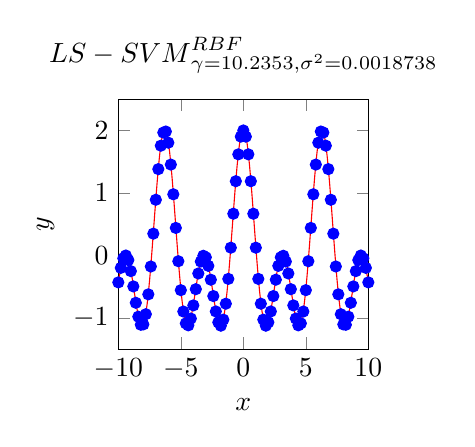
\begin{tikzpicture}

\begin{axis}[%
width=1.25in,
height=1.25in,
scale only axis,
xmin=-10,
xmax=10,
ymin=-1.5,
ymax=2.5,
xlabel={$x$},
ylabel={$y$},
title={$\text{LS-SVM}_{\gamma\text{=10.2353,}\sigma{}^\text{2}\text{=0.0018738}}^{\text{RBF}}$}
]
\addplot [color=red,solid,forget plot]
  table[row sep=crcr]{%
-10	-0.382794158226064\\
-9.9	-0.31542840514059\\
-9.8	-0.209290617485432\\
-9.7	-0.104436022691509\\
-9.6	-0.0297589748378465\\
-9.5	0.00663716354359287\\
-9.4	0.0096355322687327\\
-9.3	-0.0149546002203966\\
-9.2	-0.0652342563197698\\
-9.1	-0.140837854254202\\
-9	-0.239461306292531\\
-8.9	-0.356018924144576\\
-8.8	-0.483820578485325\\
-8.7	-0.615793609533385\\
-8.6	-0.744898148294766\\
-8.5	-0.864093769334848\\
-8.4	-0.966407044022721\\
-8.3	-1.0452424072567\\
-8.2	-1.09477353299107\\
-8.1	-1.11025545510458\\
-8	-1.08822758507005\\
-7.9	-1.02665004337803\\
-7.8	-0.925003225144367\\
-7.7	-0.784344808013278\\
-7.6	-0.607305745057128\\
-7.5	-0.398016940131312\\
-7.4	-0.161971365179353\\
-7.3	0.0941685724729631\\
-7.2	0.362809341644915\\
-7.1	0.635702051778293\\
-7	0.904246204539089\\
-6.9	1.15980985134934\\
-6.8	1.39405324457815\\
-6.7	1.5992429595825\\
-6.6	1.76854412486773\\
-6.5	1.89627939379904\\
-6.4	1.97814454725007\\
-6.3	2.0113722309383\\
-6.2	1.99483734071776\\
-6.1	1.92909988617777\\
-6	1.81638364981747\\
-5.9	1.66049149332931\\
-5.8	1.46666065143462\\
-5.7	1.24136371057889\\
-5.6	0.992063106422413\\
-5.5	0.726928801642829\\
-5.4	0.454530248655517\\
-5.3	0.183514741825927\\
-5.2	-0.077715217428287\\
-5.1	-0.321312901377876\\
-5	-0.540274524746607\\
-4.9	-0.728691409255073\\
-4.8	-0.881957361232854\\
-4.7	-0.996923276280318\\
-4.6	-1.07199309754855\\
-4.5	-1.10715759762228\\
-4.4	-1.10396493557649\\
-4.3	-1.06542946074504\\
-4.2	-0.99588269352447\\
-4.1	-0.900772712260995\\
-4	-0.786420223182846\\
-3.9	-0.659741305127812\\
-3.8	-0.527948134891837\\
-3.7	-0.39823985962466\\
-3.6	-0.277496156059067\\
-3.5	-0.171985887578727\\
-3.4	-0.0871026445990545\\
-3.3	-0.0271378567542622\\
-3.2	0.00489935934604218\\
-3.1	0.00740834402301428\\
-3	-0.0197360605220089\\
-2.9	-0.0751782694699391\\
-2.8	-0.156138730201734\\
-2.7	-0.258530422037382\\
-2.6	-0.377130379499935\\
-2.5	-0.505799315297361\\
-2.4	-0.637740473378351\\
-2.3	-0.765787251583269\\
-2.2	-0.8827079608175\\
-2.1	-0.981515380634931\\
-2	-1.05576855790684\\
-1.9	-1.09985458457369\\
-1.8	-1.1092388711787\\
-1.7	-1.08067367367067\\
-1.6	-1.01235628301824\\
-1.5	-0.904030284131657\\
-1.4	-0.757025553665023\\
-1.3	-0.574235104495459\\
-1.2	-0.360029401752693\\
-1.1	-0.12011126997515\\
-1	0.138683115310734\\
-0.9	0.40862950105121\\
-0.799999999999999	0.681397589224331\\
-0.699999999999999	0.948358843672728\\
-0.6	1.20090804265209\\
-0.5	1.43078598202661\\
-0.399999999999999	1.63039066740169\\
-0.299999999999999	1.79306476951503\\
-0.199999999999999	1.91334803900266\\
-0.0999999999999996	1.98718474728669\\
0	2.01207798600701\\
0.0999999999999996	1.98718474728669\\
0.199999999999999	1.91334803900266\\
0.299999999999999	1.79306476951503\\
0.399999999999999	1.63039066740169\\
0.5	1.43078598202661\\
0.6	1.20090804265209\\
0.699999999999999	0.948358843672728\\
0.799999999999999	0.681397589224331\\
0.9	0.40862950105121\\
1	0.138683115310734\\
1.1	-0.12011126997515\\
1.2	-0.360029401752693\\
1.3	-0.574235104495459\\
1.4	-0.757025553665023\\
1.5	-0.904030284131658\\
1.6	-1.01235628301824\\
1.7	-1.08067367367067\\
1.8	-1.1092388711787\\
1.9	-1.09985458457369\\
2	-1.05576855790684\\
2.1	-0.981515380634931\\
2.2	-0.8827079608175\\
2.3	-0.765787251583269\\
2.4	-0.637740473378351\\
2.5	-0.505799315297361\\
2.6	-0.377130379499935\\
2.7	-0.258530422037382\\
2.8	-0.156138730201734\\
2.9	-0.0751782694699391\\
3	-0.0197360605220089\\
3.1	0.00740834402301428\\
3.2	0.00489935934604217\\
3.3	-0.0271378567542622\\
3.4	-0.0871026445990545\\
3.5	-0.171985887578727\\
3.6	-0.277496156059067\\
3.7	-0.39823985962466\\
3.8	-0.527948134891836\\
3.9	-0.659741305127812\\
4	-0.786420223182846\\
4.1	-0.900772712260995\\
4.2	-0.99588269352447\\
4.3	-1.06542946074504\\
4.4	-1.10396493557649\\
4.5	-1.10715759762228\\
4.6	-1.07199309754855\\
4.7	-0.996923276280318\\
4.8	-0.881957361232854\\
4.9	-0.728691409255073\\
5	-0.540274524746607\\
5.1	-0.321312901377876\\
5.2	-0.0777152174282869\\
5.3	0.183514741825927\\
5.4	0.454530248655517\\
5.5	0.726928801642829\\
5.6	0.992063106422413\\
5.7	1.24136371057889\\
5.8	1.46666065143462\\
5.9	1.66049149332931\\
6	1.81638364981747\\
6.1	1.92909988617777\\
6.2	1.99483734071777\\
6.3	2.0113722309383\\
6.4	1.97814454725007\\
6.5	1.89627939379904\\
6.6	1.76854412486773\\
6.7	1.59924295958251\\
6.8	1.39405324457815\\
6.9	1.15980985134934\\
7	0.904246204539089\\
7.1	0.635702051778293\\
7.2	0.362809341644915\\
7.3	0.094168572472963\\
7.4	-0.161971365179353\\
7.5	-0.398016940131312\\
7.6	-0.607305745057127\\
7.7	-0.784344808013277\\
7.8	-0.925003225144366\\
7.9	-1.02665004337803\\
8	-1.08822758507005\\
8.1	-1.11025545510458\\
8.2	-1.09477353299107\\
8.3	-1.0452424072567\\
8.4	-0.966407044022721\\
8.5	-0.864093769334848\\
8.6	-0.744898148294766\\
8.7	-0.615793609533385\\
8.8	-0.483820578485325\\
8.9	-0.356018924144576\\
9	-0.239461306292531\\
9.1	-0.140837854254202\\
9.2	-0.0652342563197698\\
9.3	-0.0149546002203966\\
9.4	0.00963553226873268\\
9.5	0.00663716354359287\\
9.6	-0.0297589748378465\\
9.7	-0.104436022691509\\
9.8	-0.209290617485432\\
9.9	-0.31542840514059\\
10	-0.382794158226064\\
};
\addplot [color=blue,only marks,mark=*,mark options={solid},forget plot]
  table[row sep=crcr]{%
-10	-0.43098946726306\\
-9.8	-0.199040176459257\\
-9.6	-0.0454675090972562\\
-9.4	-0.000920685447996283\\
-9.2	-0.0742034490193951\\
-9	-0.250813553640597\\
-8.8	-0.495349259142413\\
-8.6	-0.757398242051853\\
-8.4	-0.979967241528048\\
-8.2	-1.10910282152591\\
-8	-1.103159514132\\
-7.8	-0.940222204621165\\
-7.6	-0.622477140428825\\
-7.4	-0.17680515538033\\
-7.2	0.348533958318501\\
-7	0.890639472551138\\
-6.8	1.38110148280297\\
-6.6	1.75611654959898\\
-6.4	1.96601748445563\\
-6.2	1.98273439930208\\
-6	1.80402424538286\\
-5.8	1.45380914670929\\
-5.6	0.978570742329\\
-5.4	0.440362969487297\\
-5.2	-0.0924675861268539\\
-5	-0.555409343613226\\
-4.8	-0.897188872354681\\
-4.6	-1.08699614833922\\
-4.4	-1.11842588404008\\
-4.2	-1.00954947545738\\
-4	-0.799143654672225\\
-3.8	-0.539707869332161\\
-3.6	-0.288407101801892\\
-3.4	-0.0974007022296354\\
-3.2	-0.00510985703656031\\
-3	-0.0298222099500793\\
-2.8	-0.166656462158408\\
-2.6	-0.388372082068571\\
-2.4	-0.6498947321018\\
-2.2	-0.895833987233766\\
-2	-1.06979045741075\\
-1.8	-1.12396051102723\\
-1.6	-1.02749429809604\\
-1.4	-0.772255197768418\\
-1.2	-0.37503596106457\\
-1	0.124155469320997\\
-0.799999999999999	0.66750718704588\\
-0.6	1.18769336938635\\
-0.399999999999999	1.61776770335005\\
-0.199999999999999	1.90112757184413\\
0	2\\
0.199999999999999	1.90112757184413\\
0.399999999999999	1.61776770335005\\
0.6	1.18769336938635\\
0.799999999999999	0.66750718704588\\
1	0.124155469320997\\
1.2	-0.37503596106457\\
1.4	-0.772255197768418\\
1.6	-1.02749429809604\\
1.8	-1.12396051102723\\
2	-1.06979045741075\\
2.2	-0.895833987233766\\
2.4	-0.6498947321018\\
2.6	-0.388372082068571\\
2.8	-0.166656462158408\\
3	-0.0298222099500793\\
3.2	-0.00510985703656031\\
3.4	-0.0974007022296354\\
3.6	-0.288407101801892\\
3.8	-0.539707869332161\\
4	-0.799143654672225\\
4.2	-1.00954947545738\\
4.4	-1.11842588404008\\
4.6	-1.08699614833922\\
4.8	-0.897188872354681\\
5	-0.555409343613226\\
5.2	-0.0924675861268539\\
5.4	0.440362969487297\\
5.6	0.978570742329\\
5.8	1.45380914670929\\
6	1.80402424538286\\
6.2	1.98273439930208\\
6.4	1.96601748445563\\
6.6	1.75611654959898\\
6.8	1.38110148280297\\
7	0.890639472551138\\
7.2	0.348533958318501\\
7.4	-0.17680515538033\\
7.6	-0.622477140428825\\
7.8	-0.940222204621165\\
8	-1.103159514132\\
8.2	-1.10910282152591\\
8.4	-0.979967241528048\\
8.6	-0.757398242051853\\
8.8	-0.495349259142413\\
9	-0.250813553640597\\
9.2	-0.0742034490193951\\
9.4	-0.000920685447996283\\
9.6	-0.0454675090972562\\
9.8	-0.199040176459257\\
10	-0.43098946726306\\
};
\end{axis}
\end{tikzpicture}%
\end{document}
% This file was created by matlab2tikz.
% Minimal pgfplots version: 1.3
%
%The latest updates can be retrieved from
%  http://www.mathworks.com/matlabcentral/fileexchange/22022-matlab2tikz
%where you can also make suggestions and rate matlab2tikz.
%
\documentclass[tikz]{standalone}
\usepackage{pgfplots}
\usepackage{grffile}
\pgfplotsset{compat=newest}
\usetikzlibrary{plotmarks}
\usepackage{amsmath}

\begin{document}
\definecolor{mycolor1}{rgb}{0.00000,0.44700,0.74100}%
\definecolor{mycolor2}{rgb}{0.85000,0.32500,0.09800}%
%
\begin{tikzpicture}

\begin{axis}[%
width=1.25in,
height=1.25in,
scale only axis,
xmin=-10,
xmax=10,
ymin=-1.5,
ymax=2.5,
xlabel={$x$},
ylabel={$y$},
legend style={legend cell align=left,align=left,draw=white!15!black}
]
\addplot [color=mycolor1,only marks,mark=*,mark options={solid}]
  table[row sep=crcr]{%
-9.9	-0.307869340810925\\
-9.7	-0.110072555965846\\
-9.5	-0.00846753800970923\\
-9.3	-0.0232031325135535\\
-9.1	-0.151369131839189\\
-8.9	-0.367479006452697\\
-8.7	-0.627703045668925\\
-8.5	-0.877175240736421\\
-8.3	-1.05920488021701\\
-8.1	-1.12491664409803\\
-7.9	-1.04176973451283\\
-7.7	-0.799579054849314\\
-7.5	-0.413052595023795\\
-7.3	0.0795926259688397\\
-7.1	0.621754943518725\\
-6.9	1.1465399780744\\
-6.7	1.58657623178879\\
-6.5	1.88403440717822\\
-6.3	1.99929322188442\\
-6.1	1.91690208251722\\
-5.9	1.64791090973487\\
-5.7	1.22820365118705\\
-5.5	0.713095472279311\\
-5.3	0.169036145407331\\
-5.1	-0.33628790931422\\
-4.9	-0.743913902682179\\
-4.7	-1.0120817054981\\
-4.5	-1.12192606131546\\
-4.3	-1.07951921939999\\
-4.1	-0.913978807517104\\
-3.9	-0.67197688363749\\
-3.7	-0.409552704136017\\
-3.5	-0.182554432947492\\
-3.3	-0.0372471779503353\\
-3.1	-0.00259305325006209\\
-2.9	-0.085438648208272\\
-2.7	-0.269379266074428\\
-2.5	-0.517481430083707\\
-2.3	-0.778428548214879\\
-2.1	-0.995106925940557\\
-1.9	-1.11425727877792\\
-1.7	-1.09564268687499\\
-1.5	-0.919255294932742\\
-1.3	-0.589389924744358\\
-1.1	-0.134904995829767\\
-0.9	0.394407873577576\\
-0.699999999999999	0.934809330184731\\
-0.5	1.41788486775851\\
-0.299999999999999	1.78067210403529\\
-0.0999999999999996	1.97507074311927\\
0.0999999999999996	1.97507074311927\\
0.299999999999999	1.78067210403529\\
0.5	1.41788486775851\\
0.699999999999999	0.934809330184731\\
0.9	0.394407873577576\\
1.1	-0.134904995829767\\
1.3	-0.589389924744358\\
1.5	-0.919255294932742\\
1.7	-1.09564268687499\\
1.9	-1.11425727877792\\
2.1	-0.995106925940557\\
2.3	-0.778428548214879\\
2.5	-0.517481430083707\\
2.7	-0.269379266074428\\
2.9	-0.085438648208272\\
3.1	-0.00259305325006209\\
3.3	-0.0372471779503353\\
3.5	-0.182554432947492\\
3.7	-0.409552704136017\\
3.9	-0.67197688363749\\
4.1	-0.913978807517104\\
4.3	-1.07951921939999\\
4.5	-1.12192606131546\\
4.7	-1.0120817054981\\
4.9	-0.743913902682179\\
5.1	-0.33628790931422\\
5.3	0.169036145407331\\
5.5	0.713095472279311\\
5.7	1.22820365118705\\
5.9	1.64791090973487\\
6.1	1.91690208251722\\
6.3	1.99929322188442\\
6.5	1.88403440717822\\
6.7	1.58657623178879\\
6.9	1.1465399780744\\
7.1	0.621754943518725\\
7.3	0.0795926259688397\\
7.5	-0.413052595023795\\
7.7	-0.799579054849314\\
7.9	-1.04176973451283\\
8.1	-1.12491664409803\\
8.3	-1.05920488021701\\
8.5	-0.877175240736421\\
8.7	-0.627703045668925\\
8.9	-0.367479006452697\\
9.1	-0.151369131839189\\
9.3	-0.0232031325135535\\
9.5	-0.00846753800970923\\
9.7	-0.110072555965846\\
9.9	-0.307869340810925\\
};

\addplot [color=mycolor2,only marks,mark=+,mark options={solid}]
  table[row sep=crcr]{%
-9.9	-0.31542840514059\\
-9.7	-0.104436022691509\\
-9.5	0.00663716354359287\\
-9.3	-0.0149546002203966\\
-9.1	-0.140837854254202\\
-8.9	-0.356018924144576\\
-8.7	-0.615793609533385\\
-8.5	-0.864093769334848\\
-8.3	-1.0452424072567\\
-8.1	-1.11025545510458\\
-7.9	-1.02665004337803\\
-7.7	-0.784344808013278\\
-7.5	-0.398016940131312\\
-7.3	0.0941685724729631\\
-7.1	0.635702051778293\\
-6.9	1.15980985134934\\
-6.7	1.5992429595825\\
-6.5	1.89627939379904\\
-6.3	2.0113722309383\\
-6.1	1.92909988617777\\
-5.9	1.66049149332931\\
-5.7	1.24136371057889\\
-5.5	0.726928801642829\\
-5.3	0.183514741825927\\
-5.1	-0.321312901377876\\
-4.9	-0.728691409255073\\
-4.7	-0.996923276280318\\
-4.5	-1.10715759762228\\
-4.3	-1.06542946074504\\
-4.1	-0.900772712260995\\
-3.9	-0.659741305127812\\
-3.7	-0.39823985962466\\
-3.5	-0.171985887578727\\
-3.3	-0.0271378567542622\\
-3.1	0.00740834402301428\\
-2.9	-0.0751782694699391\\
-2.7	-0.258530422037382\\
-2.5	-0.505799315297361\\
-2.3	-0.765787251583269\\
-2.1	-0.981515380634931\\
-1.9	-1.09985458457369\\
-1.7	-1.08067367367067\\
-1.5	-0.904030284131657\\
-1.3	-0.574235104495459\\
-1.1	-0.12011126997515\\
-0.9	0.40862950105121\\
-0.699999999999999	0.948358843672728\\
-0.5	1.43078598202661\\
-0.299999999999999	1.79306476951503\\
-0.0999999999999996	1.98718474728669\\
0.0999999999999996	1.98718474728669\\
0.299999999999999	1.79306476951503\\
0.5	1.43078598202661\\
0.699999999999999	0.948358843672728\\
0.9	0.40862950105121\\
1.1	-0.12011126997515\\
1.3	-0.574235104495459\\
1.5	-0.904030284131658\\
1.7	-1.08067367367067\\
1.9	-1.09985458457369\\
2.1	-0.981515380634931\\
2.3	-0.765787251583269\\
2.5	-0.505799315297361\\
2.7	-0.258530422037382\\
2.9	-0.0751782694699391\\
3.1	0.00740834402301428\\
3.3	-0.0271378567542622\\
3.5	-0.171985887578727\\
3.7	-0.39823985962466\\
3.9	-0.659741305127812\\
4.1	-0.900772712260995\\
4.3	-1.06542946074504\\
4.5	-1.10715759762228\\
4.7	-0.996923276280318\\
4.9	-0.728691409255073\\
5.1	-0.321312901377876\\
5.3	0.183514741825927\\
5.5	0.726928801642829\\
5.7	1.24136371057889\\
5.9	1.66049149332931\\
6.1	1.92909988617777\\
6.3	2.0113722309383\\
6.5	1.89627939379904\\
6.7	1.59924295958251\\
6.9	1.15980985134934\\
7.1	0.635702051778293\\
7.3	0.094168572472963\\
7.5	-0.398016940131312\\
7.7	-0.784344808013277\\
7.9	-1.02665004337803\\
8.1	-1.11025545510458\\
8.3	-1.0452424072567\\
8.5	-0.864093769334848\\
8.7	-0.615793609533385\\
8.9	-0.356018924144576\\
9.1	-0.140837854254202\\
9.3	-0.0149546002203966\\
9.5	0.00663716354359287\\
9.7	-0.104436022691509\\
9.9	-0.31542840514059\\
};
\end{axis}
\end{tikzpicture}%
\end{document}
% This file was created by matlab2tikz.
% Minimal pgfplots version: 1.3
%
%The latest updates can be retrieved from
%  http://www.mathworks.com/matlabcentral/fileexchange/22022-matlab2tikz
%where you can also make suggestions and rate matlab2tikz.
%
\documentclass[tikz]{standalone}
\usepackage{pgfplots}
\usepackage{grffile}
\pgfplotsset{compat=newest}
\usetikzlibrary{plotmarks}
\usepackage{amsmath}

\begin{document}
\begin{tikzpicture}

\begin{axis}[%
width=1.25in,
height=1.25in,
scale only axis,
xmin=-5,
xmax=0,
xlabel={$\sigma^2$},
xmajorgrids,
ymin=0,
ymax=10,
ylabel={$\gamma$},
ymajorgrids,
zmin=0,
zmax=10,
zmajorgrids,
view={90}{90},
axis x line*=bottom,
axis y line*=left,
axis z line*=left
]

\addplot3[%
surf,
shader=flat,
colormap={mymap}{[1pt] rgb(0pt)=(0.2081,0.1663,0.5292); rgb(1pt)=(0.211624,0.189781,0.577676); rgb(2pt)=(0.212252,0.213771,0.626971); rgb(3pt)=(0.2081,0.2386,0.677086); rgb(4pt)=(0.195905,0.264457,0.7279); rgb(5pt)=(0.170729,0.291938,0.779248); rgb(6pt)=(0.125271,0.324243,0.830271); rgb(7pt)=(0.0591333,0.359833,0.868333); rgb(8pt)=(0.0116952,0.38751,0.881957); rgb(9pt)=(0.00595714,0.408614,0.882843); rgb(10pt)=(0.0165143,0.4266,0.878633); rgb(11pt)=(0.0328524,0.443043,0.871957); rgb(12pt)=(0.0498143,0.458571,0.864057); rgb(13pt)=(0.0629333,0.47369,0.855438); rgb(14pt)=(0.0722667,0.488667,0.8467); rgb(15pt)=(0.0779429,0.503986,0.838371); rgb(16pt)=(0.0793476,0.520024,0.831181); rgb(17pt)=(0.0749429,0.537543,0.826271); rgb(18pt)=(0.0640571,0.556986,0.823957); rgb(19pt)=(0.0487714,0.577224,0.822829); rgb(20pt)=(0.0343429,0.596581,0.819852); rgb(21pt)=(0.0265,0.6137,0.8135); rgb(22pt)=(0.0238905,0.628662,0.803762); rgb(23pt)=(0.0230905,0.641786,0.791267); rgb(24pt)=(0.0227714,0.653486,0.776757); rgb(25pt)=(0.0266619,0.664195,0.760719); rgb(26pt)=(0.0383714,0.674271,0.743552); rgb(27pt)=(0.0589714,0.683757,0.725386); rgb(28pt)=(0.0843,0.692833,0.706167); rgb(29pt)=(0.113295,0.7015,0.685857); rgb(30pt)=(0.145271,0.709757,0.664629); rgb(31pt)=(0.180133,0.717657,0.642433); rgb(32pt)=(0.217829,0.725043,0.619262); rgb(33pt)=(0.258643,0.731714,0.595429); rgb(34pt)=(0.302171,0.737605,0.571186); rgb(35pt)=(0.348167,0.742433,0.547267); rgb(36pt)=(0.395257,0.7459,0.524443); rgb(37pt)=(0.44201,0.748081,0.503314); rgb(38pt)=(0.487124,0.749062,0.483976); rgb(39pt)=(0.530029,0.749114,0.466114); rgb(40pt)=(0.570857,0.748519,0.44939); rgb(41pt)=(0.609852,0.747314,0.433686); rgb(42pt)=(0.6473,0.7456,0.4188); rgb(43pt)=(0.683419,0.743476,0.404433); rgb(44pt)=(0.71841,0.741133,0.390476); rgb(45pt)=(0.752486,0.7384,0.376814); rgb(46pt)=(0.785843,0.735567,0.363271); rgb(47pt)=(0.818505,0.732733,0.34979); rgb(48pt)=(0.850657,0.7299,0.336029); rgb(49pt)=(0.882433,0.727433,0.3217); rgb(50pt)=(0.913933,0.725786,0.306276); rgb(51pt)=(0.944957,0.726114,0.288643); rgb(52pt)=(0.973895,0.731395,0.266648); rgb(53pt)=(0.993771,0.745457,0.240348); rgb(54pt)=(0.999043,0.765314,0.216414); rgb(55pt)=(0.995533,0.786057,0.196652); rgb(56pt)=(0.988,0.8066,0.179367); rgb(57pt)=(0.978857,0.827143,0.163314); rgb(58pt)=(0.9697,0.848138,0.147452); rgb(59pt)=(0.962586,0.870514,0.1309); rgb(60pt)=(0.958871,0.8949,0.113243); rgb(61pt)=(0.959824,0.921833,0.0948381); rgb(62pt)=(0.9661,0.951443,0.0755333); rgb(63pt)=(0.9763,0.9831,0.0538)},
mesh/rows=100]
table[row sep=crcr,header=false] {%
%
-5	0	9.71913607767262\\
-5	0.101010101010101	9.71911750564431\\
-5	0.202020202020202	9.71904418634401\\
-5	0.303030303030303	9.71879791694858\\
-5	0.404040404040404	9.7180818123259\\
-5	0.505050505050505	9.7162509394907\\
-5	0.606060606060606	9.71207761892269\\
-5	0.707070707070707	9.70349079909844\\
-5	0.808080808080808	9.68736500946506\\
-5	0.909090909090909	9.65944957142862\\
-5	1.01010101010101	9.61450894316157\\
-5	1.11111111111111	9.54669336749995\\
-5	1.21212121212121	9.45009473822307\\
-5	1.31313131313131	9.31939083107305\\
-5	1.41414141414141	9.15046009897336\\
-5	1.51515151515152	8.9408640471654\\
-5	1.61616161616162	8.69013698312136\\
-5	1.71717171717172	8.39987770380502\\
-5	1.81818181818182	8.07368504121225\\
-5	1.91919191919192	7.71700099733868\\
-5	2.02020202020202	7.33691091130872\\
-5	2.12121212121212	6.94190387004145\\
-5	2.22222222222222	6.54154058932441\\
-5	2.32323232323232	6.14594517349589\\
-5	2.42424242424242	5.76506363860231\\
-5	2.52525252525253	5.40772353151497\\
-5	2.62626262626263	5.08065291162341\\
-5	2.72727272727273	4.7877076396922\\
-5	2.82828282828283	4.52954980553097\\
-5	2.92929292929293	4.30390056437419\\
-5	3.03030303030303	4.10630624653053\\
-5	3.13131313131313	3.93119429348256\\
-5	3.23232323232323	3.77292749194009\\
-5	3.33333333333333	3.62660953115934\\
-5	3.43434343434343	3.4885161490052\\
-5	3.53535353535354	3.35616259586319\\
-5	3.63636363636364	3.22811616900113\\
-5	3.73737373737374	3.10369662354881\\
-5	3.83838383838384	2.9826835158267\\
-5	3.93939393939394	2.86509571613909\\
-5	4.04040404040404	2.75105602808426\\
-5	4.14141414141414	2.64072259193151\\
-5	4.24242424242424	2.53426060975256\\
-5	4.34343434343434	2.43183363775986\\
-5	4.44444444444444	2.33360273365613\\
-5	4.54545454545455	2.2397284093262\\
-5	4.64646464646465	2.15037372580039\\
-5	4.74747474747475	2.06570816729336\\
-5	4.84848484848485	1.98591233528186\\
-5	4.94949494949495	1.91118362604005\\
-5	5.05050505050505	1.84174311369983\\
-5	5.15151515151515	1.77784391698977\\
-5	5.25252525252525	1.71978139767602\\
-5	5.35353535353535	1.66790562786053\\
-5	5.45454545454545	1.62263667549202\\
-5	5.55555555555556	1.58448339741348\\
-5	5.65656565656566	1.55406660283488\\
-5	5.75757575757576	1.53214766307313\\
-5	5.85858585858586	1.51966389791168\\
-5	5.95959595959596	1.5177723543103\\
-5	6.06060606060606	1.52790386459116\\
-5	6.16161616161616	1.55182940492681\\
-5	6.26262626262626	1.59174048221436\\
-5	6.36363636363636	1.65034395125362\\
-5	6.46464646464646	1.7309681302233\\
-5	6.56565656565657	1.83766924237365\\
-5	6.66666666666667	1.97531165568672\\
-5	6.76767676767677	2.14956735369417\\
-5	6.86868686868687	2.36673489197302\\
-5	6.96969696969697	2.63321700746984\\
-5	7.07070707070707	2.95444100975846\\
-5	7.17171717171717	3.33302583056566\\
-5	7.27272727272727	3.76622725461807\\
-5	7.37373737373737	4.2432604247124\\
-5	7.47474747474747	4.74388776505789\\
-5	7.57575757575758	5.24001570264461\\
-5	7.67676767676768	5.70110740936049\\
-5	7.77777777777778	6.10205980317231\\
-5	7.87878787878788	6.43023673373301\\
-5	7.97979797979798	6.68822881517376\\
-5	8.08080808080808	6.89114742998409\\
-5	8.18181818181818	7.06055550358695\\
-5	8.28282828282828	7.21869414860415\\
-5	8.38383838383838	7.3849216894615\\
-5	8.48484848484848	7.57344650989021\\
-5	8.58585858585859	7.79104669628234\\
-5	8.68686868686869	8.03552862169154\\
-5	8.78787878787879	8.29668877762188\\
-5	8.88888888888889	8.55976448412853\\
-5	8.98989898989899	8.80934281835338\\
-5	9.09090909090909	9.03210457300771\\
-5	9.19191919191919	9.21848909899515\\
-5	9.29292929292929	9.36388121975823\\
-5	9.39393939393939	9.46911977743927\\
-5	9.49494949494949	9.53971958832904\\
-5	9.5959595959596	9.58389607753167\\
-5	9.6969696969697	9.61029331846618\\
-5	9.7979797979798	9.62630675103364\\
-5	9.8989898989899	9.63729997148607\\
-5	10	9.64653377687649\\
-4.94949494949495	0	9.71913553273757\\
-4.94949494949495	0.101010101010101	9.71911481061148\\
-4.94949494949495	0.202020202020202	9.71903300308032\\
-4.94949494949495	0.303030303030303	9.71875822289079\\
-4.94949494949495	0.404040404040404	9.71795921429561\\
-4.94949494949495	0.505050505050505	9.71591637993825\\
-4.94949494949495	0.606060606060606	9.71125991095614\\
-4.94949494949495	0.707070707070707	9.70167898881465\\
-4.94949494949495	0.808080808080808	9.68368630554105\\
-4.94949494949495	0.909090909090909	9.65253908025972\\
-4.94949494949495	1.01010101010101	9.60239565369832\\
-4.94949494949495	1.11111111111111	9.52672905067613\\
-4.94949494949495	1.21212121212121	9.41894721417478\\
-4.94949494949495	1.31313131313131	9.27311188457066\\
-4.94949494949495	1.41414141414141	9.08462484731077\\
-4.94949494949495	1.51515151515152	8.85076714226605\\
-4.94949494949495	1.61616161616162	8.57102524209201\\
-4.94949494949495	1.71717171717172	8.24720023534336\\
-4.94949494949495	1.81818181818182	7.88334941093546\\
-4.94949494949495	1.91919191919192	7.48563294404459\\
-4.94949494949495	2.02020202020202	7.06211886753633\\
-4.94949494949495	2.12121212121212	6.62254210478146\\
-4.94949494949495	2.22222222222222	6.17794517386064\\
-4.94949494949495	2.32323232323232	5.74009233085246\\
-4.94949494949495	2.42424242424242	5.32058513170202\\
-4.94949494949495	2.52525252525253	4.92972455142994\\
-4.94949494949495	2.62626262626263	4.57532077638409\\
-4.94949494949495	2.72727272727273	4.26176254315805\\
-4.94949494949495	2.82828282828283	3.98964400231237\\
-4.94949494949495	2.92929292929293	3.75609148106349\\
-4.94949494949495	3.03030303030303	3.55570186650517\\
-4.94949494949495	3.13131313131313	3.38181012420421\\
-4.94949494949495	3.23232323232323	3.22773193977893\\
-4.94949494949495	3.33333333333333	3.08769329720255\\
-4.94949494949495	3.43434343434343	2.95731076749716\\
-4.94949494949495	3.53535353535354	2.83364778363676\\
-4.94949494949495	3.63636363636364	2.71498197901506\\
-4.94949494949495	3.73737373737374	2.60045171368628\\
-4.94949494949495	3.83838383838384	2.48971753942583\\
-4.94949494949495	3.93939393939394	2.38271036093417\\
-4.94949494949495	4.04040404040404	2.27947830970724\\
-4.94949494949495	4.14141414141414	2.18010980645011\\
-4.94949494949495	4.24242424242424	2.08470210181173\\
-4.94949494949495	4.34343434343434	1.99335166557609\\
-4.94949494949495	4.44444444444444	1.90615322624955\\
-4.94949494949495	4.54545454545455	1.82320179315828\\
-4.94949494949495	4.64646464646465	1.74459577940731\\
-4.94949494949495	4.74747474747475	1.6704407914925\\
-4.94949494949495	4.84848484848485	1.60085410245284\\
-4.94949494949495	4.94949494949495	1.53596995927731\\
-4.94949494949495	5.05050505050505	1.47594593215319\\
-4.94949494949495	5.15151515151515	1.42097056294369\\
-4.94949494949495	5.25252525252525	1.37127263308959\\
-4.94949494949495	5.35353535353535	1.32713245401412\\
-4.94949494949495	5.45454545454545	1.28889569158744\\
-4.94949494949495	5.55555555555556	1.256990378643\\
-4.94949494949495	5.65656565656566	1.23194795897116\\
-4.94949494949495	5.75757575757576	1.21442946109189\\
-4.94949494949495	5.85858585858586	1.20525824322488\\
-4.94949494949495	5.95959595959596	1.20546120328296\\
-4.94949494949495	6.06060606060606	1.21632091115499\\
-4.94949494949495	6.16161616161616	1.23944173762753\\
-4.94949494949495	6.26262626262626	1.2768335295036\\
-4.94949494949495	6.36363636363636	1.33101623630578\\
-4.94949494949495	6.46464646464646	1.40514712296662\\
-4.94949494949495	6.56565656565657	1.50316686038676\\
-4.94949494949495	6.66666666666667	1.62994837788941\\
-4.94949494949495	6.76767676767677	1.79140714109273\\
-4.94949494949495	6.86868686868687	1.99448544042693\\
-4.94949494949495	6.96969696969697	2.24684919009047\\
-4.94949494949495	7.07070707070707	2.5560401053974\\
-4.94949494949495	7.17171717171717	2.9277609708921\\
-4.94949494949495	7.27272727272727	3.36308373726255\\
-4.94949494949495	7.37373737373737	3.85490051519954\\
-4.94949494949495	7.47474747474747	4.38498686651481\\
-4.94949494949495	7.57575757575758	4.9240219345931\\
-4.94949494949495	7.67676767676768	5.43644206200377\\
-4.94949494949495	7.77777777777778	5.88947467138068\\
-4.94949494949495	7.87878787878788	6.26269807226185\\
-4.94949494949495	7.97979797979798	6.55343083232698\\
-4.94949494949495	8.08080808080808	6.77527100568702\\
-4.94949494949495	8.18181818181818	6.95129218606767\\
-4.94949494949495	8.28282828282828	7.10659801011641\\
-4.94949494949495	8.38383838383838	7.26382796134848\\
-4.94949494949495	8.48484848484848	7.44101601201917\\
-4.94949494949495	8.58585858585859	7.64921727998253\\
-4.94949494949495	8.68686868686869	7.8897921063615\\
-4.94949494949495	8.78787878787879	8.15406603098111\\
-4.94949494949495	8.88888888888889	8.4267717417977\\
-4.94949494949495	8.98989898989899	8.69106342277354\\
-4.94949494949495	9.09090909090909	8.93209679159825\\
-4.94949494949495	9.19191919191919	9.13864394726706\\
-4.94949494949495	9.29292929292929	9.30402843257122\\
-4.94949494949495	9.39393939393939	9.42694011194893\\
-4.94949494949495	9.49494949494949	9.51136793066104\\
-4.94949494949495	9.5959595959596	9.56506664489687\\
-4.94949494949495	9.6969696969697	9.59716189769916\\
-4.94949494949495	9.7979797979798	9.61603621477622\\
-4.94949494949495	9.8989898989899	9.62814215753041\\
-4.94949494949495	10	9.63768962713475\\
-4.8989898989899	0	9.71913500221671\\
-4.8989898989899	0.101010101010101	9.71911218686555\\
-4.8989898989899	0.202020202020202	9.71902211562753\\
-4.8989898989899	0.303030303030303	9.71871957878905\\
-4.8989898989899	0.404040404040404	9.71783985913242\\
-4.8989898989899	0.505050505050505	9.71559066989481\\
-4.8989898989899	0.606060606060606	9.71046383237399\\
-4.8989898989899	0.707070707070707	9.69991510319084\\
-4.8989898989899	0.808080808080808	9.68010490812664\\
-4.8989898989899	0.909090909090909	9.64581138113\\
-4.8989898989899	1.01010101010101	9.59060277908702\\
-4.8989898989899	1.11111111111111	9.50729282469058\\
-4.8989898989899	1.21212121212121	9.3886236087947\\
-4.8989898989899	1.31313131313131	9.22805715671073\\
-4.8989898989899	1.41414141414141	9.02053129449421\\
-4.8989898989899	1.51515151515152	8.76305438819433\\
-4.8989898989899	1.61616161616162	8.45506756508768\\
-4.8989898989899	1.71717171717172	8.09857230529498\\
-4.8989898989899	1.81818181818182	7.69808059350674\\
-4.8989898989899	1.91919191919192	7.26046934555759\\
-4.8989898989899	2.02020202020202	6.79479543332712\\
-4.8989898989899	2.12121212121212	6.31205803965328\\
-4.8989898989899	2.22222222222222	5.82481375791959\\
-4.8989898989899	2.32323232323232	5.34650886083604\\
-4.8989898989899	2.42424242424242	4.89044069410452\\
-4.8989898989899	2.52525252525253	4.46840638917059\\
-4.8989898989899	2.62626262626263	4.08928874303176\\
-4.8989898989899	2.72727272727273	3.7579611384186\\
-4.8989898989899	2.82828282828283	3.47486864563114\\
-4.8989898989899	2.92929292929293	3.23644481207714\\
-4.8989898989899	3.03030303030303	3.03624176143919\\
-4.8989898989899	3.13131313131313	2.86642442072518\\
-4.8989898989899	3.23232323232323	2.71920817127184\\
-4.8989898989899	3.33333333333333	2.58791100088749\\
-4.8989898989899	3.43434343434343	2.46747691781386\\
-4.8989898989899	3.53535353535354	2.35451428955391\\
-4.8989898989899	3.63636363636364	2.24701292192957\\
-4.8989898989899	3.73737373737374	2.14393394811496\\
-4.8989898989899	3.83838383838384	2.04482443194713\\
-4.8989898989899	3.93939393939394	1.94953408616323\\
-4.8989898989899	4.04040404040404	1.85804453525792\\
-4.8989898989899	4.14141414141414	1.77038408828967\\
-4.8989898989899	4.24242424242424	1.68659301191633\\
-4.8989898989899	4.34343434343434	1.6067128511373\\
-4.8989898989899	4.44444444444444	1.53078517092259\\
-4.8989898989899	4.54545454545455	1.45885346123121\\
-4.8989898989899	4.64646464646465	1.39096611119105\\
-4.8989898989899	4.74747474747475	1.32717994549041\\
-4.8989898989899	4.84848484848485	1.26756431453702\\
-4.8989898989899	4.94949494949495	1.21220587585179\\
-4.8989898989899	5.05050505050505	1.16121425720008\\
-4.8989898989899	5.15151515151515	1.11472883119383\\
-4.8989898989899	5.25252525252525	1.07292688126098\\
-4.8989898989899	5.35353535353535	1.03603350876238\\
-4.8989898989899	5.45454545454545	1.00433372756166\\
-4.8989898989899	5.55555555555556	0.97818732734845\\
-4.8989898989899	5.65656565656566	0.958047280662063\\
-4.8989898989899	5.75757575757576	0.944482751555488\\
-4.8989898989899	5.85858585858586	0.938208177613322\\
-4.8989898989899	5.95959595959596	0.940120488556353\\
-4.8989898989899	6.06060606060606	0.951347329904991\\
-4.8989898989899	6.16161616161616	0.973310168444557\\
-4.8989898989899	6.26262626262626	1.00780724510245\\
-4.8989898989899	6.36363636363636	1.05712216405507\\
-4.8989898989899	6.46464646464646	1.12416369530319\\
-4.8989898989899	6.56565656565657	1.21263955541044\\
-4.8989898989899	6.66666666666667	1.32725845433844\\
-4.8989898989899	6.76767676767677	1.4739348290182\\
-4.8989898989899	6.86868686868687	1.65992963860437\\
-4.8989898989899	6.96969696969697	1.89378462957333\\
-4.8989898989899	7.07070707070707	2.18478646838136\\
-4.8989898989899	7.17171717171717	2.54155366426639\\
-4.8989898989899	7.27272727272727	2.96929720323054\\
-4.8989898989899	7.37373737373737	3.46566992752722\\
-4.8989898989899	7.47474747474747	4.01626158343736\\
-4.8989898989899	7.57575757575758	4.59246036115006\\
-4.8989898989899	7.67676767676768	5.15486535117437\\
-4.8989898989899	7.77777777777778	5.66288394840956\\
-4.8989898989899	7.87878787878788	6.08688094758102\\
-4.8989898989899	7.97979797979798	6.41689292321638\\
-4.8989898989899	8.08080808080808	6.66339160385317\\
-4.8989898989899	8.18181818181818	6.85029675103639\\
-4.8989898989899	8.28282828282828	7.00551070875907\\
-4.8989898989899	8.38383838383838	7.15479506664699\\
-4.8989898989899	8.48484848484848	7.31970967502042\\
-4.8989898989899	8.58585858585859	7.51579032590981\\
-4.8989898989899	8.68686868686869	7.74894584369092\\
-4.8989898989899	8.78787878787879	8.01313181292901\\
-4.8989898989899	8.88888888888889	8.29294887064217\\
-4.8989898989899	8.98989898989899	8.56983951164602\\
-4.8989898989899	9.09090909090909	8.82725504406192\\
-4.8989898989899	9.19191919191919	9.05261854476681\\
-4.8989898989899	9.29292929292929	9.23766519023997\\
-4.8989898989899	9.39393939393939	9.37902546920063\\
-4.8989898989899	9.49494949494949	9.47876405123677\\
-4.8989898989899	9.5959595959596	9.54360682075034\\
-4.8989898989899	9.6969696969697	9.58274248372131\\
-4.8989898989899	9.7979797979798	9.60535889302269\\
-4.8989898989899	9.8989898989899	9.61898681650335\\
-4.8989898989899	10	9.62887059828238\\
-4.84848484848485	0	9.71913449903844\\
-4.84848484848485	0.101010101010101	9.71910969834527\\
-4.84848484848485	0.202020202020202	9.71901178930486\\
-4.84848484848485	0.303030303030303	9.71868292637169\\
-4.84848484848485	0.404040404040404	9.71772665543382\\
-4.84848484848485	0.505050505050505	9.71528174667421\\
-4.84848484848485	0.606060606060606	9.70970878302377\\
-4.84848484848485	0.707070707070707	9.69824212681299\\
-4.84848484848485	0.808080808080808	9.6767080932048\\
-4.84848484848485	0.909090909090909	9.63943042298607\\
-4.84848484848485	1.01010101010101	9.57941770259748\\
-4.84848484848485	1.11111111111111	9.48885833492314\\
-4.84848484848485	1.21212121212121	9.35986288292659\\
-4.84848484848485	1.31313131313131	9.18532458909983\\
-4.84848484848485	1.41414141414141	8.95974132374454\\
-4.84848484848485	1.51515151515152	8.67986317417171\\
-4.84848484848485	1.61616161616162	8.34508937927569\\
-4.84848484848485	1.71717171717172	7.95761463666502\\
-4.84848484848485	1.81818181818182	7.5223898320039\\
-4.84848484848485	1.91919191919192	7.04698770594614\\
-4.84848484848485	2.02020202020202	6.54143227632964\\
-4.84848484848485	2.12121212121212	6.0179684651004\\
-4.84848484848485	2.22222222222222	5.49065337682448\\
-4.84848484848485	2.32323232323232	4.97460458794607\\
-4.84848484848485	2.42424242424242	4.48480089795317\\
-4.84848484848485	2.52525252525253	4.03450876917756\\
-4.84848484848485	2.62626262626263	3.63363745947794\\
-4.84848484848485	2.72727272727273	3.28747946083526\\
-4.84848484848485	2.82828282828283	2.99625429562963\\
-4.84848484848485	2.92929292929293	2.75562926784923\\
-4.84848484848485	3.03030303030303	2.55805451184075\\
-4.84848484848485	3.13131313131313	2.39449106688403\\
-4.84848484848485	3.23232323232323	2.25604295631529\\
-4.84848484848485	3.33333333333333	2.13512580731946\\
-4.84848484848485	3.43434343434343	2.02602562012569\\
-4.84848484848485	3.53535353535354	1.92491290672922\\
-4.84848484848485	3.63636363636364	1.82950607451244\\
-4.84848484848485	3.73737373737374	1.7386037387537\\
-4.84848484848485	3.83838383838384	1.65165292433966\\
-4.84848484848485	3.93939393939394	1.56843516992358\\
-4.84848484848485	4.04040404040404	1.48887880409852\\
-4.84848484848485	4.14141414141414	1.41296570804594\\
-4.84848484848485	4.24242424242424	1.34069334282366\\
-4.84848484848485	4.34343434343434	1.27206290005158\\
-4.84848484848485	4.44444444444444	1.20707761472571\\
-4.84848484848485	4.54545454545455	1.14574443435818\\
-4.84848484848485	4.64646464646465	1.08807674471976\\
-4.84848484848485	4.74747474747475	1.03409756784158\\
-4.84848484848485	4.84848484848485	0.983843194345212\\
-4.84848484848485	4.94949494949495	0.937367371865609\\
-4.84848484848485	5.05050505050505	0.894746218879445\\
-4.84848484848485	5.15151515151515	0.856084057547101\\
-4.84848484848485	5.25252525252525	0.821520391258001\\
-4.84848484848485	5.35353535353535	0.791238303789002\\
-4.84848484848485	5.45454545454545	0.765474636314097\\
-4.84848484848485	5.55555555555556	0.744532422436358\\
-4.84848484848485	5.65656565656566	0.728796258947673\\
-4.84848484848485	5.75757575757576	0.718751604825176\\
-4.84848484848485	5.85858585858586	0.715009489680698\\
-4.84848484848485	5.95959595959596	0.718338835762744\\
-4.84848484848485	6.06060606060606	0.729709598333124\\
-4.84848484848485	6.16161616161616	0.750351204102741\\
-4.84848484848485	6.26262626262626	0.781832227338623\\
-4.84848484848485	6.36363636363636	0.826168661913397\\
-4.84848484848485	6.46464646464646	0.885969049529278\\
-4.84848484848485	6.56565656565657	0.964624089992851\\
-4.84848484848485	6.66666666666667	1.0665439237865\\
-4.84848484848485	6.76767676767677	1.19743312704297\\
-4.84848484848485	6.86868686868687	1.36456173815348\\
-4.84848484848485	6.96969696969697	1.57692302310794\\
-4.84848484848485	7.07070707070707	1.84504176017116\\
-4.84848484848485	7.17171717171717	2.18000005967786\\
-4.84848484848485	7.27272727272727	2.59105142976785\\
-4.84848484848485	7.37373737373737	3.08128980936087\\
-4.84848484848485	7.47474747474747	3.64181784788564\\
-4.84848484848485	7.57575757575758	4.24705144706713\\
-4.84848484848485	7.67676767676768	4.85564814955163\\
-4.84848484848485	7.77777777777778	5.41971451057828\\
-4.84848484848485	7.87878787878788	5.89933599160219\\
-4.84848484848485	7.97979797979798	6.27517804445775\\
-4.84848484848485	8.08080808080808	6.55254469882411\\
-4.84848484848485	8.18181818181818	6.7551647263361\\
-4.84848484848485	8.28282828282828	6.91367998148507\\
-4.84848484848485	8.38383838383838	7.05697591488317\\
-4.84848484848485	8.48484848484848	7.20968197007742\\
-4.84848484848485	8.58585858585859	7.39154577462511\\
-4.84848484848485	8.68686868686869	7.61380112060538\\
-4.84848484848485	8.78787878787879	7.87450783206655\\
-4.84848484848485	8.88888888888889	8.1590189610203\\
-4.84848484848485	8.98989898989899	8.44681225783448\\
-4.84848484848485	9.09090909090909	8.71901540834906\\
-4.84848484848485	9.19191919191919	8.96165284776\\
-4.84848484848485	9.29292929292929	9.16541950186427\\
-4.84848484848485	9.39393939393939	9.32535223691445\\
-4.84848484848485	9.49494949494949	9.44149171543349\\
-4.84848484848485	9.5959595959596	9.51901480145763\\
-4.84848484848485	9.6969696969697	9.56664909600433\\
-4.84848484848485	9.7979797979798	9.59408928428821\\
-4.84848484848485	9.8989898989899	9.60985568598822\\
-4.84848484848485	10	9.62025963288485\\
-4.7979797979798	0	9.71913403347363\\
-4.7979797979798	0.101010101010101	9.71910739584617\\
-4.7979797979798	0.202020202020202	9.71900223489267\\
-4.7979797979798	0.303030303030303	9.71864901378594\\
-4.7979797979798	0.404040404040404	9.71762191390768\\
-4.7979797979798	0.505050505050505	9.71499591600056\\
-4.7979797979798	0.606060606060606	9.70901017493048\\
-4.7979797979798	0.707070707070707	9.69669420837375\\
-4.7979797979798	0.808080808080808	9.67356519632826\\
-4.7979797979798	0.909090909090909	9.63352645341447\\
-4.7979797979798	1.01010101010101	9.56906873281059\\
-4.7979797979798	1.11111111111111	9.47180186346878\\
-4.7979797979798	1.21212121212121	9.33325209421822\\
-4.7979797979798	1.31313131313131	9.14578642277979\\
-4.7979797979798	1.41414141414141	8.90349573116528\\
-4.7979797979798	1.51515151515152	8.60289143256427\\
-4.7979797979798	1.61616161616162	8.24333498337934\\
-4.7979797979798	1.71717171717172	7.82720259767014\\
-4.7979797979798	1.81818181818182	7.35985789157264\\
-4.7979797979798	1.91919191919192	6.84953132788466\\
-4.7979797979798	2.02020202020202	6.30716714821243\\
-4.7979797979798	2.12121212121212	5.74620320582822\\
-4.7979797979798	2.22222222222222	5.18214037005077\\
-4.7979797979798	2.32323232323232	4.63170720045918\\
-4.7979797979798	2.42424242424242	4.11149900367167\\
-4.7979797979798	2.52525252525253	3.63618097580166\\
-4.7979797979798	2.62626262626263	3.2166140338776\\
-4.7979797979798	2.72727272727273	2.85843658855902\\
-4.7979797979798	2.82828282828283	2.56158062508321\\
-4.7979797979798	2.92929292929293	2.3209062376986\\
-4.7979797979798	3.03030303030303	2.12774717834956\\
-4.7979797979798	3.13131313131313	1.97187154832229\\
-4.7979797979798	3.23232323232323	1.84330120894803\\
-4.7979797979798	3.33333333333333	1.73358728214315\\
-4.7979797979798	3.43434343434343	1.6363958565534\\
-4.7979797979798	3.53535353535354	1.54749286166664\\
-4.7979797979798	3.63636363636364	1.46435225552649\\
-4.7979797979798	3.73737373737374	1.38563167146589\\
-4.7979797979798	3.83838383838384	1.31069604565878\\
-4.7979797979798	3.93939393939394	1.23927477313245\\
-4.7979797979798	4.04040404040404	1.17125806647763\\
-4.7979797979798	4.14141414141414	1.10659621336542\\
-4.7979797979798	4.24242424242424	1.04525851062802\\
-4.7979797979798	4.34343434343434	0.987220241179646\\
-4.7979797979798	4.44444444444444	0.932460515500621\\
-4.7979797979798	4.54545454545455	0.88096367145589\\
-4.7979797979798	4.64646464646465	0.83272173436532\\
-4.7979797979798	4.74747474747475	0.787737268210567\\
-4.7979797979798	4.84848484848485	0.746026543173411\\
-4.7979797979798	4.94949494949495	0.707623119978975\\
-4.7979797979798	5.05050505050505	0.672581991282205\\
-4.7979797979798	5.15151515151515	0.640984424196941\\
-4.7979797979798	5.25252525252525	0.612943656285612\\
-4.7979797979798	5.35353535353535	0.588611626446573\\
-4.7979797979798	5.45454545454545	0.568186986289586\\
-4.7979797979798	5.55555555555556	0.551924762373899\\
-4.7979797979798	5.65656565656566	0.5401482672845\\
-4.7979797979798	5.75757575757576	0.533264244233597\\
-4.7979797979798	5.85858585858586	0.531782834448138\\
-4.7979797979798	5.95959595959596	0.536344818631822\\
-4.7979797979798	6.06060606060606	0.547759700091813\\
-4.7979797979798	6.16161616161616	0.567059515321349\\
-4.7979797979798	6.26262626262626	0.595574703078735\\
-4.7979797979798	6.36363636363636	0.63503987690412\\
-4.7979797979798	6.46464646464646	0.687738848987571\\
-4.7979797979798	6.56565656565657	0.756699375891504\\
-4.7979797979798	6.66666666666667	0.845947479279894\\
-4.7979797979798	6.76767676767677	0.960825076579385\\
-4.7979797979798	6.86868686868687	1.10835431444561\\
-4.7979797979798	6.96969696969697	1.29757969630632\\
-4.7979797979798	7.07070707070707	1.53970405780203\\
-4.7979797979798	7.17171717171717	1.84761888355842\\
-4.7979797979798	7.27272727272727	2.23411692277635\\
-4.7979797979798	7.37373737373737	2.70786979340984\\
-4.7979797979798	7.47474747474747	3.26681198938247\\
-4.7979797979798	7.57575757575758	3.89086432696212\\
-4.7979797979798	7.67676767676768	4.53933292000475\\
-4.7979797979798	7.77777777777778	5.15834117801946\\
-4.7979797979798	7.87878787878788	5.69715891525203\\
-4.7979797979798	7.97979797979798	6.12509719922371\\
-4.7979797979798	8.08080808080808	6.43989654607838\\
-4.7979797979798	8.18181818181818	6.66354391033537\\
-4.7979797979798	8.28282828282828	6.82921271265987\\
-4.7979797979798	8.38383838383838	6.96917497206035\\
-4.7979797979798	8.48484848484848	7.1107592400707\\
-4.7979797979798	8.58585858585859	7.27718072431223\\
-4.7979797979798	8.68686868686869	7.48521454773423\\
-4.7979797979798	8.78787878787879	7.73862678699919\\
-4.7979797979798	8.88888888888889	8.02513187186201\\
-4.7979797979798	8.98989898989899	8.32242789535296\\
-4.7979797979798	9.09090909090909	8.6084002114824\\
-4.7979797979798	9.19191919191919	8.86702193432879\\
-4.7979797979798	9.29292929292929	9.08824261122645\\
-4.7979797979798	9.39393939393939	9.26623214254529\\
-4.7979797979798	9.49494949494949	9.39932244799523\\
-4.7979797979798	9.5959595959596	9.49082219362479\\
-4.7979797979798	9.6969696969697	9.54843198218348\\
-4.7979797979798	9.7979797979798	9.58193458452621\\
-4.7979797979798	9.8989898989899	9.60066008205484\\
-4.7979797979798	10	9.61196164602542\\
-4.74747474747475	0	9.71913361248287\\
-4.74747474747475	0.101010101010101	9.71910531379269\\
-4.74747474747475	0.202020202020202	9.71899359523794\\
-4.74747474747475	0.303030303030303	9.71861834805516\\
-4.74747474747475	0.404040404040404	9.71752720053317\\
-4.74747474747475	0.505050505050505	9.71473745129677\\
-4.74747474747475	0.606060606060606	9.70837845290487\\
-4.74747474747475	0.707070707070707	9.69529449061844\\
-4.74747474747475	0.808080808080808	9.67072320654295\\
-4.74747474747475	0.909090909090909	9.62818774179355\\
-4.74747474747475	1.01010101010101	9.55971059532689\\
-4.74747474747475	1.11111111111111	9.45637841771093\\
-4.74747474747475	1.21212121212121	9.30918909196405\\
-4.74747474747475	1.31313131313131	9.11003377188677\\
-4.74747474747475	1.41414141414141	8.85263538373207\\
-4.74747474747475	1.51515151515152	8.53328976540135\\
-4.74747474747475	1.61616161616162	8.15132501771038\\
-4.74747474747475	1.71717171717172	7.70928376829335\\
-4.74747474747475	1.81818181818182	7.21290835394152\\
-4.74747474747475	1.91919191919192	6.6710355187023\\
-4.74747474747475	2.02020202020202	6.09546263073846\\
-4.74747474747475	2.12121212121212	5.50073956070054\\
-4.74747474747475	2.22222222222222	4.90371829003466\\
-4.74747474747475	2.32323232323232	4.32263680695674\\
-4.74747474747475	2.42424242424242	3.77560080558747\\
-4.74747474747475	2.52525252525253	3.27857010963823\\
-4.74747474747475	2.62626262626263	2.84326424901847\\
-4.74747474747475	2.72727272727273	2.47559599985135\\
-4.74747474747475	2.82828282828283	2.1751688260679\\
-4.74747474747475	2.92929292929293	1.9360294945841\\
-4.74747474747475	3.03030303030303	1.74842158561699\\
-4.74747474747475	3.13131313131313	1.60097012237251\\
-4.74747474747475	3.23232323232323	1.482676481464\\
-4.74747474747475	3.33333333333333	1.38428945208679\\
-4.74747474747475	3.43434343434343	1.29890989632079\\
-4.74747474747475	3.53535353535354	1.2219428431867\\
-4.74747474747475	3.63636363636364	1.15065079829325\\
-4.74747474747475	3.73737373737374	1.08357520113669\\
-4.74747474747475	3.83838383838384	1.02001840587889\\
-4.74747474747475	3.93939393939394	0.959674206036234\\
-4.74747474747475	4.04040404040404	0.902409681053716\\
-4.74747474747475	4.14141414141414	0.848157626949316\\
-4.74747474747475	4.24242424242424	0.796872666518585\\
-4.74747474747475	4.34343434343434	0.748517153672108\\
-4.74747474747475	4.44444444444444	0.70305859877091\\
-4.74747474747475	4.54545454545455	0.660470850140589\\
-4.74747474747475	4.64646464646465	0.620736337681603\\
-4.74747474747475	4.74747474747475	0.583848612945518\\
-4.74747474747475	4.84848484848485	0.549815060456486\\
-4.74747474747475	4.94949494949495	0.518659844859639\\
-4.74747474747475	5.05050505050505	0.490427184627514\\
-4.74747474747475	5.15151515151515	0.465185018375817\\
-4.74747474747475	5.25252525252525	0.443029110367087\\
-4.74747474747475	5.35353535353535	0.424087657390381\\
-4.74747474747475	5.45454545454545	0.408526539282094\\
-4.74747474747475	5.55555555555556	0.396555544627209\\
-4.74747474747475	5.65656565656566	0.388436258134919\\
-4.74747474747475	5.75757575757576	0.384492862062902\\
-4.74747474747475	5.85858585858586	0.385127878963472\\
-4.74747474747475	5.95959595959596	0.390845791602423\\
-4.74747474747475	6.06060606060606	0.402288392765115\\
-4.74747474747475	6.16161616161616	0.420286565784461\\
-4.74747474747475	6.26262626262626	0.445934078574511\\
-4.74747474747475	6.36363636363636	0.480690217825157\\
-4.74747474747475	6.46464646464646	0.526520097463325\\
-4.74747474747475	6.56565656565657	0.586084350051028\\
-4.74747474747475	6.66666666666667	0.662992861660373\\
-4.74747474747475	6.76767676767677	0.762137505695888\\
-4.74747474747475	6.86868686868687	0.890109584264227\\
-4.74747474747475	6.96969696969697	1.05567335682918\\
-4.74747474747475	7.07070707070707	1.27017592091893\\
-4.74747474747475	7.17171717171717	1.5475721473447\\
-4.74747474747475	7.27272727272727	1.90337618230104\\
-4.74747474747475	7.37373737373737	2.35139050325456\\
-4.74747474747475	7.47474747474747	2.89705927564609\\
-4.74747474747475	7.57575757575758	3.52810624443577\\
-4.74747474747475	7.67676767676768	4.20765788392986\\
-4.74747474747475	7.77777777777778	4.87810184567542\\
-4.74747474747475	7.87878787878788	5.47804656579515\\
-4.74747474747475	7.97979797979798	5.96373654642691\\
-4.74747474747475	8.08080808080808	6.32275179331608\\
-4.74747474747475	8.18181818181818	6.57321458281292\\
-4.74747474747475	8.28282828282828	6.75023933881116\\
-4.74747474747475	8.38383838383838	6.88996550361705\\
-4.74747474747475	8.48484848484848	7.0224172070892\\
-4.74747474747475	8.58585858585859	7.17327890576052\\
-4.74747474747475	8.68686868686869	7.36427638827314\\
-4.74747474747475	8.78787878787879	7.60613301786592\\
-4.74747474747475	8.88888888888889	7.89120125680114\\
-4.74747474747475	8.98989898989899	8.19647176257731\\
-4.74747474747475	9.09090909090909	8.49577014668822\\
-4.74747474747475	9.19191919191919	8.76972781324751\\
-4.74747474747475	9.29292929292929	9.00723936670135\\
-4.74747474747475	9.39393939393939	9.20230911283832\\
-4.74747474747475	9.49494949494949	9.35228996277204\\
-4.74747474747475	9.5959595959596	9.45866768727264\\
-4.74747474747475	9.6969696969697	9.52762594383776\\
-4.74747474747475	9.7979797979798	9.56851824400033\\
-4.74747474747475	9.8989898989899	9.59119941923858\\
-4.74747474747475	10	9.60397635212596\\
-4.6969696969697	0	9.71913323962491\\
-4.6969696969697	0.101010101010101	9.71910346978496\\
-4.6969696969697	0.202020202020202	9.71898594337389\\
-4.6969696969697	0.303030303030303	9.71859118840471\\
-4.6969696969697	0.404040404040404	9.71744331594681\\
-4.6969696969697	0.505050505050505	9.71450853743119\\
-4.6969696969697	0.606060606060606	9.70781895705312\\
-4.6969696969697	0.707070707070707	9.69405480570668\\
-4.6969696969697	0.808080808080808	9.668206147856\\
-4.6969696969697	0.909090909090909	9.62345941739403\\
-4.6969696969697	1.01010101010101	9.5514223961524\\
-4.6969696969697	1.11111111111111	9.44271837387755\\
-4.6969696969697	1.21212121212121	9.287877280996\\
-4.6969696969697	1.31313131313131	9.07836884542596\\
-4.6969696969697	1.41414141414141	8.80759016011791\\
-4.6969696969697	1.51515151515152	8.47164633228739\\
-4.6969696969697	1.61616161616162	8.06983656508739\\
-4.6969696969697	1.71717171717172	7.60485268335956\\
-4.6969696969697	1.81818181818182	7.08277682151649\\
-4.6969696969697	1.91919191919192	6.51299184955931\\
-4.6969696969697	2.02020202020202	5.9080674007066\\
-4.6969696969697	2.12121212121212	5.28356462035242\\
-4.6969696969697	2.22222222222222	4.65756814762811\\
-4.6969696969697	2.32323232323232	4.04969423622847\\
-4.6969696969697	2.42424242424242	3.4794241306353\\
-4.6969696969697	2.52525252525253	2.963886854253\\
-4.6969696969697	2.62626262626263	2.51555978059791\\
-4.6969696969697	2.72727272727273	2.14056750659681\\
-4.6969696969697	2.82828282828283	1.83816790245722\\
-4.6969696969697	2.92929292929293	1.60162078284333\\
-4.6969696969697	3.03030303030303	1.42013899181872\\
-4.6969696969697	3.13131313131313	1.2812824899499\\
-4.6969696969697	3.23232323232323	1.17311476570674\\
-4.6969696969697	3.33333333333333	1.08565863823865\\
-4.6969696969697	3.43434343434343	1.01151334847427\\
-4.6969696969697	3.53535353535354	0.945771809341343\\
-4.6969696969697	3.63636363636364	0.885520573999705\\
-4.6969696969697	3.73737373737374	0.829210545879\\
-4.6969696969697	3.83838383838384	0.776100933452384\\
-4.6969696969697	3.93939393939394	0.725865885087907\\
-4.6969696969697	4.04040404040404	0.678363440980597\\
-4.6969696969697	4.14141414141414	0.633521912504372\\
-4.6969696969697	4.24242424242424	0.591293515443341\\
-4.6969696969697	4.34343434343434	0.551639404244026\\
-4.6969696969697	4.44444444444444	0.514526847304936\\
-4.6969696969697	4.54545454545455	0.479930327127691\\
-4.6969696969697	4.64646464646465	0.447833651517463\\
-4.6969696969697	4.74747474747475	0.418232183093699\\
-4.6969696969697	4.84848484848485	0.391134974453128\\
-4.6969696969697	4.94949494949495	0.366566788794616\\
-4.6969696969697	5.05050505050505	0.344569984060767\\
-4.6969696969697	5.15151515151515	0.325206181984242\\
-4.6969696969697	5.25252525252525	0.308557626252112\\
-4.6969696969697	5.35353535353535	0.294728227140757\\
-4.6969696969697	5.45454545454545	0.283844559522592\\
-4.6969696969697	5.55555555555556	0.276057578801354\\
-4.6969696969697	5.65656565656566	0.27154652977461\\
-4.6969696969697	5.75757575757576	0.270527303551457\\
-4.6969696969697	5.85858585858586	0.273268084613774\\
-4.6969696969697	5.95959595959596	0.280115286850922\\
-4.6969696969697	6.06060606060606	0.291532532176138\\
-4.6969696969697	6.16161616161616	0.308155209185712\\
-4.6969696969697	6.26262626262626	0.330863651912095\\
-4.6969696969697	6.36363636363636	0.360879800030682\\
-4.6969696969697	6.46464646464646	0.39989558764444\\
-4.6969696969697	6.56565656565657	0.450246111673866\\
-4.6969696969697	6.66666666666667	0.515146269252567\\
-4.6969696969697	6.76767676767677	0.599014428733931\\
-4.6969696969697	6.86868686868687	0.707906347361287\\
-4.6969696969697	6.96969696969697	0.85006524325639\\
-4.6969696969697	7.07070707070707	1.03653194797102\\
-4.6969696969697	7.17171717171717	1.28159472015144\\
-4.6969696969697	7.27272727272727	1.60249986416255\\
-4.6969696969697	7.37373737373737	2.01723148974439\\
-4.6969696969697	7.47474747474747	2.53861919166446\\
-4.6969696969697	7.57575757575758	3.16389479104749\\
-4.6969696969697	7.67676767676768	3.86347022183811\\
-4.6969696969697	7.77777777777778	4.57927507994484\\
-4.6969696969697	7.87878787878788	5.24031768393807\\
-4.6969696969697	7.97979797979798	5.78846764042206\\
-4.6969696969697	8.08080808080808	6.19851058244393\\
-4.6969696969697	8.18181818181818	6.48207326110369\\
-4.6969696969697	8.28282828282828	6.6750154286134\\
-4.6969696969697	8.38383838383838	6.81782604861854\\
-4.6969696969697	8.48484848484848	6.94376932663637\\
-4.6969696969697	8.58585858585859	7.08015164822851\\
-4.6969696969697	8.68686868686869	7.2522753451195\\
-4.6969696969697	8.78787878787879	7.47817547008497\\
-4.6969696969697	8.88888888888889	7.75735916096047\\
-4.6969696969697	8.98989898989899	8.06834217727448\\
-4.6969696969697	9.09090909090909	8.38075722445054\\
-4.6969696969697	9.19191919191919	8.67021460065499\\
-4.6969696969697	9.29292929292929	8.92341178722426\\
-4.6969696969697	9.39393939393939	9.13446925402492\\
-4.6969696969697	9.49494949494949	9.30072928003142\\
-4.6969696969697	9.5959595959596	9.42237053022858\\
-4.6969696969697	9.6969696969697	9.50380855408232\\
-4.6969696969697	9.7979797979798	9.55341689302851\\
-4.6969696969697	9.8989898989899	9.58117805183497\\
-4.6969696969697	10	9.59619022833258\\
-4.64646464646465	0	9.71913291542361\\
-4.64646464646465	0.101010101010101	9.71910186641384\\
-4.64646464646465	0.202020202020202	9.71897929005156\\
-4.64646464646465	0.303030303030303	9.71856757299445\\
-4.64646464646465	0.404040404040404	9.71737037800815\\
-4.64646464646465	0.505050505050505	9.71430949603211\\
-4.64646464646465	0.606060606060606	9.70733247347569\\
-4.64646464646465	0.707070707070707	9.69297689540706\\
-4.64646464646465	0.808080808080808	9.66601755672629\\
-4.64646464646465	0.909090909090909	9.61934812339091\\
-4.64646464646465	1.01010101010101	9.54421577968635\\
-4.64646464646465	1.11111111111111	9.43084092261738\\
-4.64646464646465	1.21212121212121	9.26934659928909\\
-4.64646464646465	1.31313131313131	9.05083611694839\\
-4.64646464646465	1.41414141414141	8.76842329628488\\
-4.64646464646465	1.51515151515152	8.41804755491439\\
-4.64646464646465	1.61616161616162	7.99898346296257\\
-4.64646464646465	1.71717171717172	7.5140539586012\\
-4.64646464646465	1.81818181818182	6.96963998145576\\
-4.64646464646465	1.91919191919192	6.37560627047684\\
-4.64646464646465	2.02020202020202	5.74520670203167\\
-4.64646464646465	2.12121212121212	5.09490190078925\\
-4.64646464646465	2.22222222222222	4.44387579641408\\
-4.64646464646465	2.32323232323232	3.81297460540275\\
-4.64646464646465	2.42424242424242	3.22290447599978\\
-4.64646464646465	2.52525252525253	2.69182860543987\\
-4.64646464646465	2.62626262626263	2.23288259357225\\
-4.64646464646465	2.72727272727273	1.85235418621996\\
-4.64646464646465	2.82828282828283	1.549162861905\\
-4.64646464646465	2.92929292929293	1.31583600739837\\
-4.64646464646465	3.03030303030303	1.14063931278607\\
-4.64646464646465	3.13131313131313	1.01016112664335\\
-4.64646464646465	3.23232323232323	0.911617032487281\\
-4.64646464646465	3.33333333333333	0.834383232363299\\
-4.64646464646465	3.43434343434343	0.770622496927198\\
-4.64646464646465	3.53535353535354	0.71516556655222\\
-4.64646464646465	3.63636363636364	0.664959369394432\\
-4.64646464646465	3.73737373737374	0.618390407170626\\
-4.64646464646465	3.83838383838384	0.574694470932894\\
-4.64646464646465	3.93939393939394	0.533542362566996\\
-4.64646464646465	4.04040404040404	0.494797726936727\\
-4.64646464646465	4.14141414141414	0.458398209188216\\
-4.64646464646465	4.24242424242424	0.424306993045027\\
-4.64646464646465	4.34343434343434	0.392497263338126\\
-4.64646464646465	4.44444444444444	0.362949428414941\\
-4.64646464646465	4.54545454545455	0.335652334152963\\
-4.64646464646465	4.64646464646465	0.310605195718967\\
-4.64646464646465	4.74747474747475	0.287819091150869\\
-4.64646464646465	4.84848484848485	0.267317563593442\\
-4.64646464646465	4.94949494949495	0.249136051806093\\
-4.64646464646465	5.05050505050505	0.233319871412001\\
-4.64646464646465	5.15151515151515	0.21992055149544\\
-4.64646464646465	5.25252525252525	0.208990704347911\\
-4.64646464646465	5.35353535353535	0.200578378813123\\
-4.64646464646465	5.45454545454545	0.194722914319717\\
-4.64646464646465	5.55555555555556	0.19145525930749\\
-4.64646464646465	5.65656565656566	0.190805925763003\\
-4.64646464646465	5.75757575757576	0.192822830138748\\
-4.64646464646465	5.85858585858586	0.197599549115258\\
-4.64646464646465	5.95959595959596	0.205313020082953\\
-4.64646464646465	6.06060606060606	0.216269459590891\\
-4.64646464646465	6.16161616161616	0.230958565123889\\
-4.64646464646465	6.26262626262626	0.2501185134017\\
-4.64646464646465	6.36363636363636	0.274817394660017\\
-4.64646464646465	6.46464646464646	0.306560495311449\\
-4.64646464646465	6.56565656565657	0.347437698274991\\
-4.64646464646465	6.66666666666667	0.40033168569103\\
-4.64646464646465	6.76767676767677	0.469215332290983\\
-4.64646464646465	6.86868686868687	0.559573197258907\\
-4.64646464646465	6.96969696969697	0.67897932126247\\
-4.64646464646465	7.07070707070707	0.837830096126417\\
-4.64646464646465	7.17171717171717	1.0501148013867\\
-4.64646464646465	7.27272727272727	1.33380319971435\\
-4.64646464646465	7.37373737373737	1.70978635282661\\
-4.64646464646465	7.47474747474747	2.19736135227096\\
-4.64646464646465	7.57575757575758	2.80400267131081\\
-4.64646464646465	7.67676767676768	3.51066421024928\\
-4.64646464646465	7.77777777777778	4.26307460999548\\
-4.64646464646465	7.87878787878788	4.98291880847037\\
-4.64646464646465	7.97979797979798	5.59695988438408\\
-4.64646464646465	8.08080808080808	6.06462401632305\\
-4.64646464646465	8.18181818181818	6.3880526492117\\
-4.64646464646465	8.28282828282828	6.60194104389553\\
-4.64646464646465	8.38383838383838	6.75127967610934\\
-4.64646464646465	8.48484848484848	6.87363088321866\\
-4.64646464646465	8.58585858585859	6.9976636488858\\
-4.64646464646465	8.68686868686869	7.15045701027638\\
-4.64646464646465	8.78787878787879	7.35646359214178\\
-4.64646464646465	8.88888888888889	7.62436937820348\\
-4.64646464646465	8.98989898989899	7.93749530280653\\
-4.64646464646465	9.09090909090909	8.26242423359268\\
-4.64646464646465	9.19191919191919	8.56820363290226\\
-4.64646464646465	9.29292929292929	8.83737334739507\\
-4.64646464646465	9.39393939393939	9.06365928231155\\
-4.64646464646465	9.49494949494949	9.24525557496956\\
-4.64646464646465	9.5959595959596	9.38198943851636\\
-4.64646464646465	9.6969696969697	9.47666269651532\\
-4.64646464646465	9.7979797979798	9.5362052000454\\
-4.64646464646465	9.8989898989899	9.57023485930874\\
-4.64646464646465	10	9.58838772435604\\
-4.5959595959596	0	9.71913263801361\\
-4.5959595959596	0.101010101010101	9.7191004944539\\
-4.5959595959596	0.202020202020202	9.7189735969893\\
-4.5959595959596	0.303030303030303	9.71854736594685\\
-4.5959595959596	0.404040404040404	9.71730796704937\\
-4.5959595959596	0.505050505050505	9.71413918186164\\
-4.5959595959596	0.606060606060606	9.70691620305769\\
-4.5959595959596	0.707070707070707	9.692054557664\\
-4.5959595959596	0.808080808080808	9.66414484046118\\
-4.5959595959596	0.909090909090909	9.61583020417369\\
-4.5959595959596	1.01010101010101	9.53804928014923\\
-4.5959595959596	1.11111111111111	9.42067772213327\\
-4.5959595959596	1.21212121212121	9.25349042081992\\
-4.5959595959596	1.31313131313131	9.02727715539628\\
-4.5959595959596	1.41414141414141	8.73490938877688\\
-4.5959595959596	1.51515151515152	8.37218487486863\\
-4.5959595959596	1.61616161616162	7.93835747166391\\
-4.5959595959596	1.71717171717172	7.43636333352201\\
-4.5959595959596	1.81818181818182	6.87284155937504\\
-4.5959595959596	1.91919191919192	6.25807439936343\\
-4.5959595959596	2.02020202020202	5.60591065897506\\
-4.5959595959596	2.12121212121212	4.93359555136561\\
-4.5959595959596	2.22222222222222	4.26127399025139\\
-4.5959595959596	2.32323232323232	3.61086806345187\\
-4.5959595959596	2.42424242424242	3.00415376027016\\
-4.5959595959596	2.52525252525253	2.46019345586281\\
-4.5959595959596	2.62626262626263	1.99268878265971\\
-4.5959595959596	2.72727272727273	1.60805828534923\\
-4.5959595959596	2.82828282828283	1.30491405070081\\
-4.5959595959596	2.92929292929293	1.07513113944583\\
-4.5959595959596	3.03030303030303	0.90612997431577\\
-4.5959595959596	3.13131313131313	0.783625189484171\\
-4.5959595959596	3.23232323232323	0.694067257432127\\
-4.5959595959596	3.33333333333333	0.626255039196599\\
-4.5959595959596	3.43434343434343	0.57197383578155\\
-4.5959595959596	3.53535353535354	0.525841080288848\\
-4.5959595959596	3.63636363636364	0.484702477964253\\
-4.5959595959596	3.73737373737374	0.446909700860089\\
-4.5959595959596	3.83838383838384	0.411699010361556\\
-4.5959595959596	3.93939393939394	0.378759179221419\\
-4.5959595959596	4.04040404040404	0.34798028114196\\
-4.5959595959596	4.14141414141414	0.319330572162496\\
-4.5959595959596	4.24242424242424	0.292806235866079\\
-4.5959595959596	4.34343434343434	0.268415404112915\\
-4.5959595959596	4.44444444444444	0.246175365225319\\
-4.5959595959596	4.54545454545455	0.226113124333882\\
-4.5959595959596	4.64646464646465	0.208264994525603\\
-4.5959595959596	4.74747474747475	0.192673202582978\\
-4.5959595959596	4.84848484848485	0.179378522367028\\
-4.5959595959596	4.94949494949495	0.16840883295827\\
-4.5959595959596	5.05050505050505	0.15976488453615\\
-4.5959595959596	5.15151515151515	0.153406522672654\\
-4.5959595959596	5.25252525252525	0.149244331790192\\
-4.5959595959596	5.35353535353535	0.147141586409791\\
-4.5959595959596	5.45454545454545	0.146928683326036\\
-4.5959595959596	5.55555555555556	0.148428062577449\\
-4.5959595959596	5.65656565656566	0.151484707033837\\
-4.5959595959596	5.75757575757576	0.155997448048096\\
-4.5959595959596	5.85858585858586	0.161948943566884\\
-4.5959595959596	5.95959595959596	0.169435410155905\\
-4.5959595959596	6.06060606060606	0.178699508960899\\
-4.5959595959596	6.16161616161616	0.190170889418936\\
-4.5959595959596	6.26262626262626	0.204519222718371\\
-4.5959595959596	6.36363636363636	0.222724823384554\\
-4.5959595959596	6.46464646464646	0.246173108096\\
-4.5959595959596	6.56565656565657	0.276782548971143\\
-4.5959595959596	6.66666666666667	0.317183071882839\\
-4.5959595959596	6.76767676767677	0.370973825705449\\
-4.5959595959596	6.86868686868687	0.443103979248585\\
-4.5959595959596	6.96969696969697	0.540430860684114\\
-4.5959595959596	7.07070707070707	0.672499879915882\\
-4.5959595959596	7.17171717171717	0.852520666434962\\
-4.5959595959596	7.27272727272727	1.09828628801572\\
-4.5959595959596	7.37373737373737	1.43221075894155\\
-4.5959595959596	7.47474747474747	1.87853089991519\\
-4.5959595959596	7.57575757575758	2.45453234629144\\
-4.5959595959596	7.67676767676768	3.15412184515411\\
-4.5959595959596	7.77777777777778	3.93170424574877\\
-4.5959595959596	7.87878787878788	4.70544998521037\\
-4.5959595959596	7.97979797979798	5.3871980983665\\
-4.5959595959596	8.08080808080808	5.91857683009858\\
-4.5959595959596	8.18181818181818	6.28902564164533\\
-4.5959595959596	8.28282828282828	6.5294984047651\\
-4.5959595959596	8.38383838383838	6.68899189147305\\
-4.5959595959596	8.48484848484848	6.81066476365582\\
-4.5959595959596	8.58585858585859	6.92515777521575\\
-4.5959595959596	8.68686868686869	7.0596912837787\\
-4.5959595959596	8.78787878787879	7.24305016117874\\
-4.5959595959596	8.88888888888889	7.49384830359299\\
-4.5959595959596	8.98989898989899	7.80393462193499\\
-4.5959595959596	9.09090909090909	8.13962567049741\\
-4.5959595959596	9.19191919191919	8.46271648229604\\
-4.5959595959596	9.29292929292929	8.74911664255365\\
-4.5959595959596	9.39393939393939	8.99064022863003\\
-4.5959595959596	9.49494949494949	9.1866648598075\\
-4.5959595959596	9.5959595959596	9.33784801121482\\
-4.5959595959596	9.6969696969697	9.4460363914957\\
-4.5959595959596	9.7979797979798	9.51650473502134\\
-4.5959595959596	9.8989898989899	9.55797911542639\\
-4.5959595959596	10	9.58027621278896\\
-4.54545454545455	0	9.71913240388001\\
-4.54545454545455	0.101010101010101	9.71909933652186\\
-4.54545454545455	0.202020202020202	9.71896879205363\\
-4.54545454545455	0.303030303030303	9.71853031123021\\
-4.54545454545455	0.404040404040404	9.71725529229758\\
-4.54545454545455	0.505050505050505	9.71399543696797\\
-4.54545454545455	0.606060606060606	9.70656487147751\\
-4.54545454545455	0.707070707070707	9.69127610606397\\
-4.54545454545455	0.808080808080808	9.66256427092295\\
-4.54545454545455	0.909090909090909	9.61286108608728\\
-4.54545454545455	1.01010101010101	9.53284476493742\\
-4.54545454545455	1.11111111111111	9.41209999903579\\
-4.54545454545455	1.21212121212121	9.24010783726662\\
-4.54545454545455	1.31313131313131	9.00739344731891\\
-4.54545454545455	1.41414141414141	8.70662376444287\\
-4.54545454545455	1.51515151515152	8.33347705944717\\
-4.54545454545455	1.61616161616162	7.88718997247028\\
-4.54545454545455	1.71717171717172	7.37079495038258\\
-4.54545454545455	1.81818181818182	6.79115076207289\\
-4.54545454545455	1.91919191919192	6.15889576936515\\
-4.54545454545455	2.02020202020202	5.48838768969256\\
-4.54545454545455	2.12121212121212	4.79754467439639\\
-4.54545454545455	2.22222222222222	4.1073373839079\\
-4.54545454545455	2.32323232323232	3.44061295430634\\
-4.54545454545455	2.42424242424242	2.82006654643594\\
-4.54545454545455	2.52525252525253	2.2655315742634\\
-4.54545454545455	2.62626262626263	1.7911943878359\\
-4.54545454545455	2.72727272727273	1.40358864079316\\
-4.54545454545455	2.82828282828283	1.10107388949714\\
-4.54545454545455	2.92929292929293	0.874981894873907\\
-4.54545454545455	3.03030303030303	0.712013041269678\\
-4.54545454545455	3.13131313131313	0.59710852377156\\
-4.54545454545455	3.23232323232323	0.516014863507805\\
-4.54545454545455	3.33333333333333	0.456993627256625\\
-4.54545454545455	3.43434343434343	0.411493383656179\\
-4.54545454545455	3.53535353535354	0.373964857749257\\
-4.54545454545455	3.63636363636364	0.341199568952472\\
-4.54545454545455	3.73737373737374	0.311557623821066\\
-4.54545454545455	3.83838383838384	0.284315683955591\\
-4.54545454545455	3.93939393939394	0.259219872327625\\
-4.54545454545455	4.04040404040404	0.23622771051935\\
-4.54545454545455	4.14141414141414	0.215380668377515\\
-4.54545454545455	4.24242424242424	0.196749407028072\\
-4.54545454545455	4.34343434343434	0.180411974763106\\
-4.54545454545455	4.44444444444444	0.166442353579125\\
-4.54545454545455	4.54545454545455	0.154897582143178\\
-4.54545454545455	4.64646464646465	0.145799008095878\\
-4.54545454545455	4.74747474747475	0.139109826406591\\
-4.54545454545455	4.84848484848485	0.134716599090124\\
-4.54545454545455	4.94949494949495	0.132424174169035\\
-4.54545454545455	5.05050505050505	0.131969052694915\\
-4.54545454545455	5.15151515151515	0.133047841913739\\
-4.54545454545455	5.25252525252525	0.135351069614884\\
-4.54545454545455	5.35353535353535	0.138592601304848\\
-4.54545454545455	5.45454545454545	0.142529732945242\\
-4.54545454545455	5.55555555555556	0.146974328784377\\
-4.54545454545455	5.65656565656566	0.151798398328598\\
-4.54545454545455	5.75757575757576	0.156938264748307\\
-4.54545454545455	5.85858585858586	0.162401175942202\\
-4.54545454545455	5.95959595959596	0.168277876252932\\
-4.54545454545455	6.06060606060606	0.174764762779117\\
-4.54545454545455	6.16161616161616	0.182199832114237\\
-4.54545454545455	6.26262626262626	0.191117406509717\\
-4.54545454545455	6.36363636363636	0.20232704443249\\
-4.54545454545455	6.46464646464646	0.217021379664416\\
-4.54545454545455	6.56565656565657	0.236915916682922\\
-4.54545454545455	6.66666666666667	0.264423859547699\\
-4.54545454545455	6.76767676767677	0.302878185883275\\
-4.54545454545455	6.86868686868687	0.356839119847166\\
-4.54545454545455	6.96969696969697	0.432563151614652\\
-4.54545454545455	7.07070707070707	0.538732929681249\\
-4.54545454545455	7.17171717171717	0.687513228753664\\
-4.54545454545455	7.27272727272727	0.895833315379513\\
-4.54545454545455	7.37373737373737	1.18634031170628\\
-4.54545454545455	7.47474747474747	1.58636805556447\\
-4.54545454545455	7.57575757575758	2.12149602791435\\
-4.54545454545455	7.67676767676768	2.79958041643481\\
-4.54545454545455	7.77777777777778	3.58846971829642\\
-4.54545454545455	7.87878787878788	4.40825694255799\\
-4.54545454545455	7.97979797979798	5.15751275627842\\
-4.54545454545455	8.08080808080808	5.75789972359464\\
-4.54545454545455	8.18181818181818	6.18273668360398\\
-4.54545454545455	8.28282828282828	6.45613762548213\\
-4.54545454545455	8.38383838383838	6.62978825912078\\
-4.54545454545455	8.48484848484848	6.75355798070695\\
-4.54545454545455	8.58585858585859	6.86153134484175\\
-4.54545454545455	8.68686868686869	6.9802026488619\\
-4.54545454545455	8.78787878787879	7.13991501672773\\
-4.54545454545455	8.88888888888889	7.36819957325162\\
-4.54545454545455	8.98989898989899	7.66860078839355\\
-4.54545454545455	9.09090909090909	8.0114866388515\\
-4.54545454545455	9.19191919191919	8.35229883211117\\
-4.54545454545455	9.29292929292929	8.6579118989292\\
-4.54545454545455	9.39393939393939	8.91573458355987\\
-4.54545454545455	9.49494949494949	9.12575769448227\\
-4.54545454545455	9.5959595959596	9.29050633978699\\
-4.54545454545455	9.6969696969697	9.41198923222385\\
-4.54545454545455	9.7979797979798	9.49403403527442\\
-4.54545454545455	9.8989898989899	9.54402824067964\\
-4.54545454545455	10	9.57151710378385\\
-4.49494949494949	0	9.7191322085518\\
-4.49494949494949	0.101010101010101	9.71909837050596\\
-4.49494949494949	0.202020202020202	9.71896478349001\\
-4.49494949494949	0.303030303030303	9.71851608316946\\
-4.49494949494949	0.404040404040404	9.71721134788129\\
-4.49494949494949	0.505050505050505	9.71387551641365\\
-4.49494949494949	0.606060606060606	9.70627176974314\\
-4.49494949494949	0.707070707070707	9.69062667537016\\
-4.49494949494949	0.808080808080808	9.66124566569092\\
-4.49494949494949	0.909090909090909	9.61038407105015\\
-4.49494949494949	1.01010101010101	9.52850284880635\\
-4.49494949494949	1.11111111111111	9.40494395294849\\
-4.49494949494949	1.21212121212121	9.22894329318397\\
-4.49494949494949	1.31313131313131	8.99080528653579\\
-4.49494949494949	1.41414141414141	8.68302625450842\\
-4.49494949494949	1.51515151515152	8.30118484479592\\
-4.49494949494949	1.61616161616162	7.844503518148\\
-4.49494949494949	1.71717171717172	7.31609557257201\\
-4.49494949494949	1.81818181818182	6.7230042908443\\
-4.49494949494949	1.91919191919192	6.07616774484256\\
-4.49494949494949	2.02020202020202	5.39037298695483\\
-4.49494949494949	2.12121212121212	4.68410712846058\\
-4.49494949494949	2.22222222222222	3.97904006753044\\
-4.49494949494949	2.32323232323232	3.29880279910183\\
-4.49494949494949	2.42424242424242	2.66686935641866\\
-4.49494949494949	2.52525252525253	2.10372700225213\\
-4.49494949494949	2.62626262626263	1.62397734839207\\
-4.49494949494949	2.72727272727273	1.23426858767836\\
-4.49494949494949	2.82828282828283	0.932787375717524\\
-4.49494949494949	2.92929292929293	0.710473276756649\\
-4.49494949494949	3.03030303030303	0.553484777959999\\
-4.49494949494949	3.13131313131313	0.446119131981324\\
-4.49494949494949	3.23232323232323	0.37345248307216\\
-4.49494949494949	3.33333333333333	0.323183593136288\\
-4.49494949494949	3.43434343434343	0.286414224885267\\
-4.49494949494949	3.53535353535354	0.257465628391477\\
-4.49494949494949	3.63636363636364	0.233144670873405\\
-4.49494949494949	3.73737373737374	0.211898197263769\\
-4.49494949494949	3.83838383838384	0.19311714823814\\
-4.49494949494949	3.93939393939394	0.176667836158886\\
-4.49494949494949	4.04040404040404	0.162617496109912\\
-4.49494949494949	4.14141414141414	0.1510839775641\\
-4.49494949494949	4.24242424242424	0.142150088349075\\
-4.49494949494949	4.34343434343434	0.135811677923693\\
-4.49494949494949	4.44444444444444	0.131951651048006\\
-4.49494949494949	4.54545454545455	0.130340835887684\\
-4.49494949494949	4.64646464646465	0.130663746067821\\
-4.49494949494949	4.74747474747475	0.132559660686695\\
-4.49494949494949	4.84848484848485	0.135664855021228\\
-4.49494949494949	4.94949494949495	0.139644573394004\\
-4.49494949494949	5.05050505050505	0.144210640939619\\
-4.49494949494949	5.15151515151515	0.149126798525878\\
-4.49494949494949	5.25252525252525	0.154206325997872\\
-4.49494949494949	5.35353535353535	0.159306189918836\\
-4.49494949494949	5.45454545454545	0.164320613952774\\
-4.49494949494949	5.55555555555556	0.169175755082887\\
-4.49494949494949	5.65656565656566	0.17382644491331\\
-4.49494949494949	5.75757575757576	0.17825571683761\\
-4.49494949494949	5.85858585858586	0.182478006322767\\
-4.49494949494949	5.95959595959596	0.186547457044942\\
-4.49494949494949	6.06060606060606	0.190573754411435\\
-4.49494949494949	6.16161616161616	0.194749487040136\\
-4.49494949494949	6.26262626262626	0.19939537255702\\
-4.49494949494949	6.36363636363636	0.205032750476108\\
-4.49494949494949	6.46464646464646	0.212495779643537\\
-4.49494949494949	6.56565656565657	0.223096332976581\\
-4.49494949494949	6.66666666666667	0.238848196223064\\
-4.49494949494949	6.76767676767677	0.262741849321457\\
-4.49494949494949	6.86868686868687	0.2990517174989\\
-4.49494949494949	6.96969696969697	0.353695344184168\\
-4.49494949494949	7.07070707070707	0.434769271514764\\
-4.49494949494949	7.17171717171717	0.553471177725001\\
-4.49494949494949	7.27272727272727	0.725520843852785\\
-4.49494949494949	7.37373737373737	0.972785774780508\\
-4.49494949494949	7.47474747474747	1.32385656447311\\
-4.49494949494949	7.57575757575758	1.81033677508778\\
-4.49494949494949	7.67676767676768	2.45334650961236\\
-4.49494949494949	7.77777777777778	3.23787613750155\\
-4.49494949494949	7.87878787878788	4.09261975651632\\
-4.49494949494949	7.97979797979798	4.90665194685513\\
-4.49494949494949	8.08080808080808	5.5802000482799\\
-4.49494949494949	8.18181818181818	6.06678045628936\\
-4.49494949494949	8.28282828282828	6.38015827785607\\
-4.49494949494949	8.38383838383838	6.57258529511457\\
-4.49494949494949	8.48484848484848	6.70115722607329\\
-4.49494949494949	8.58585858585859	6.80543482819104\\
-4.49494949494949	8.68686868686869	6.91147945446081\\
-4.49494949494949	8.78787878787879	7.04850545469173\\
-4.49494949494949	8.88888888888889	7.2502606948478\\
-4.49494949494949	8.98989898989899	7.53353695942688\\
-4.49494949494949	9.09090909090909	7.87788622261716\\
-4.49494949494949	9.19191919191919	8.23540331675084\\
-4.49494949494949	9.29292929292929	8.5623780465823\\
-4.49494949494949	9.39393939393939	8.8386391632377\\
-4.49494949494949	9.49494949494949	9.06311476868109\\
-4.49494949494949	9.5959595959596	9.24066509373394\\
-4.49494949494949	9.6969696969697	9.37481029999765\\
-4.49494949494949	9.7979797979798	9.4686559748104\\
-4.49494949494949	9.8989898989899	9.52804584719079\\
-4.49494949494949	10	9.56175719967874\\
-4.44444444444444	0	9.71913204716906\\
-4.44444444444444	0.101010101010101	9.71909757237087\\
-4.44444444444444	0.202020202020202	9.71896147156181\\
-4.44444444444444	0.303030303030303	9.71850432775778\\
-4.44444444444444	0.404040404040404	9.71717504042425\\
-4.44444444444444	0.505050505050505	9.71377643646826\\
-4.44444444444444	0.606060606060606	9.70602960522107\\
-4.44444444444444	0.707070707070707	9.69009010716241\\
-4.44444444444444	0.808080808080808	9.66015621666753\\
-4.44444444444444	0.909090909090909	9.60833752863304\\
-4.44444444444444	1.01010101010101	9.52491550073465\\
-4.44444444444444	1.11111111111111	9.3990315342586\\
-4.44444444444444	1.21212121212121	9.21971900249286\\
-4.44444444444444	1.31313131313131	8.97709993811084\\
-4.44444444444444	1.41414141414141	8.66352970990556\\
-4.44444444444444	1.51515151515152	8.27450469472506\\
-4.44444444444444	1.61616161616162	7.80923576519351\\
-4.44444444444444	1.71717171717172	7.2709033758911\\
-4.44444444444444	1.81818181818182	6.66670411833884\\
-4.44444444444444	1.91919191919192	6.00782549096566\\
-4.44444444444444	2.02020202020202	5.30941255070262\\
-4.44444444444444	2.12121212121212	4.59042769638384\\
-4.44444444444444	2.22222222222222	3.87312570613562\\
-4.44444444444444	2.32323232323232	3.18179371422069\\
-4.44444444444444	2.42424242424242	2.54055814150221\\
-4.44444444444444	2.52525252525253	1.97045574483101\\
-4.44444444444444	2.62626262626263	1.48644498955637\\
-4.44444444444444	2.72727272727273	1.09529993474504\\
-4.44444444444444	2.82828282828283	0.795139431291839\\
-4.44444444444444	2.92929292929293	0.576729503970943\\
-4.44444444444444	3.03030303030303	0.425996937162419\\
-4.44444444444444	3.13131313131313	0.326866067666864\\
-4.44444444444444	3.23232323232323	0.263786144167375\\
-4.44444444444444	3.33333333333333	0.223703181569602\\
-4.44444444444444	3.43434343434343	0.197169639733578\\
-4.44444444444444	3.53535353535354	0.178320900876939\\
-4.44444444444444	3.63636363636364	0.164034259495433\\
-4.44444444444444	3.73737373737374	0.152903539351492\\
-4.44444444444444	3.83838383838384	0.144419777624742\\
-4.44444444444444	3.93939393939394	0.138439904755343\\
-4.44444444444444	4.04040404040404	0.134887300791755\\
-4.44444444444444	4.14141414141414	0.133609659463796\\
-4.44444444444444	4.24242424242424	0.134341086912196\\
-4.44444444444444	4.34343434343434	0.136730382593333\\
-4.44444444444444	4.44444444444444	0.140397711369178\\
-4.44444444444444	4.54545454545455	0.144985584590974\\
-4.44444444444444	4.64646464646465	0.15018727524896\\
-4.44444444444444	4.74747474747475	0.155754258424651\\
-4.44444444444444	4.84848484848485	0.161491748850064\\
-4.44444444444444	4.94949494949495	0.167249895731193\\
-4.44444444444444	5.05050505050505	0.17291459158931\\
-4.44444444444444	5.15151515151515	0.178399418444854\\
-4.44444444444444	5.25252525252525	0.183639120873243\\
-4.44444444444444	5.35353535353535	0.188584570130796\\
-4.44444444444444	5.45454545454545	0.193199070560972\\
-4.44444444444444	5.55555555555556	0.197455885212146\\
-4.44444444444444	5.65656565656566	0.20133696010219\\
-4.44444444444444	5.75757575757576	0.204832997056839\\
-4.44444444444444	5.85858585858586	0.207945291242309\\
-4.44444444444444	5.95959595959596	0.210690179961347\\
-4.44444444444444	6.06060606060606	0.213107673609613\\
-4.44444444444444	6.16161616161616	0.215277087380295\\
-4.44444444444444	6.26262626262626	0.217344650253894\\
-4.44444444444444	6.36363636363636	0.21957172950597\\
-4.44444444444444	6.46464646464646	0.222418181018788\\
-4.44444444444444	6.56565656565657	0.226683551384538\\
-4.44444444444444	6.66666666666667	0.233736629312879\\
-4.44444444444444	6.76767676767677	0.245860517184855\\
-4.44444444444444	6.86868686868687	0.266705771222206\\
-4.44444444444444	6.96969696969697	0.301778122102711\\
-4.44444444444444	7.07070707070707	0.35888927300751\\
-4.44444444444444	7.17171717171717	0.448724586818804\\
-4.44444444444444	7.27272727272727	0.585965958478961\\
-4.44444444444444	7.37373737373737	0.791174902077368\\
-4.44444444444444	7.47474747474747	1.09265726357089\\
-4.44444444444444	7.57575757575758	1.52548584369084\\
-4.44444444444444	7.67676767676768	2.12183396481553\\
-4.44444444444444	7.77777777777778	2.88559438219488\\
-4.44444444444444	7.87878787878788	3.76101277600035\\
-4.44444444444444	7.97979797979798	4.63393976121556\\
-4.44444444444444	8.08080808080808	5.38320908881739\\
-4.44444444444444	8.18181818181818	5.93862074053236\\
-4.44444444444444	8.28282828282828	6.29962885276129\\
-4.44444444444444	8.38383838383838	6.51626536126894\\
-4.44444444444444	8.48484848484848	6.65251226084685\\
-4.44444444444444	8.58585858585859	6.75550949334245\\
-4.44444444444444	8.68686868686869	6.85238953784281\\
-4.44444444444444	8.78787878787879	6.96940427635167\\
-4.44444444444444	8.88888888888889	7.14276122860884\\
-4.44444444444444	8.98989898989899	7.40175558554631\\
-4.44444444444444	9.09090909090909	7.73982766487938\\
-4.44444444444444	9.19191919191919	8.11085520475569\\
-4.44444444444444	9.29292929292929	8.46072006264688\\
-4.44444444444444	9.39393939393939	8.75836234672453\\
-4.44444444444444	9.49494949494949	8.99887768735454\\
-4.44444444444444	9.5959595959596	9.18900534209028\\
-4.44444444444444	9.6969696969697	9.33499073735202\\
-4.44444444444444	9.7979797979798	9.44041493756166\\
-4.44444444444444	9.8989898989899	9.5097798488404\\
-4.44444444444444	10	9.55065786520476\\
-4.39393939393939	0	9.71913191489682\\
-4.39393939393939	0.101010101010101	9.71909691820478\\
-4.39393939393939	0.202020202020202	9.71895875704502\\
-4.39393939393939	0.303030303030303	9.71849469280781\\
-4.39393939393939	0.404040404040404	9.71714528216985\\
-4.39393939393939	0.505050505050505	9.71369522873692\\
-4.39393939393939	0.606060606060606	9.70583112276017\\
-4.39393939393939	0.707070707070707	9.6896503260719\\
-4.39393939393939	0.808080808080808	9.65926328438693\\
-4.39393939393939	0.909090909090909	9.60666014519694\\
-4.39393939393939	1.01010101010101	9.52197524503701\\
-4.39393939393939	1.11111111111111	9.39418560873174\\
-4.39393939393939	1.21212121212121	9.21215860756929\\
-4.39393939393939	1.31313131313131	8.96586679055504\\
-4.39393939393939	1.41414141414141	8.64755000625349\\
-4.39393939393939	1.51515151515152	8.2526372272585\\
-4.39393939393939	1.61616161616162	7.78032991425302\\
-4.39393939393939	1.71717171717172	7.23386380537673\\
-4.39393939393939	1.81818181818182	6.62056172868676\\
-4.39393939393939	1.91919191919192	5.95181683549348\\
-4.39393939393939	2.02020202020202	5.24306983009312\\
-4.39393939393939	2.12121212121212	4.51367619216976\\
-4.39393939393939	2.22222222222222	3.78637495127309\\
-4.39393939393939	2.32323232323232	3.08599690192699\\
-4.39393939393939	2.42424242424242	2.43720964352924\\
-4.39393939393939	2.52525252525253	1.86150826721493\\
-4.39393939393939	2.62626262626263	1.37415894062922\\
-4.39393939393939	2.72727272727273	0.982080284872172\\
-4.39393939393939	2.82828282828283	0.683452363831741\\
-4.39393939393939	2.92929292929293	0.469190804385374\\
-4.39393939393939	3.03030303030303	0.325601940176731\\
-4.39393939393939	3.13131313131313	0.236971609330885\\
-4.39393939393939	3.23232323232323	0.187253242243808\\
-4.39393939393939	3.33333333333333	0.161704675505776\\
-4.39393939393939	3.43434343434343	0.149181840802222\\
-4.39393939393939	3.53535353535354	0.143127453558888\\
-4.39393939393939	3.63636363636364	0.140445187641378\\
-4.39393939393939	3.73737373737374	0.139878110526401\\
-4.39393939393939	3.83838383838384	0.140932366349136\\
-4.39393939393939	3.93939393939394	0.143357688899636\\
-4.39393939393939	4.04040404040404	0.146947571718823\\
-4.39393939393939	4.14141414141414	0.151483214211211\\
-4.39393939393939	4.24242424242424	0.156731787929101\\
-4.39393939393939	4.34343434343434	0.162463244655879\\
-4.39393939393939	4.44444444444444	0.168470589088294\\
-4.39393939393939	4.54545454545455	0.174583535044371\\
-4.39393939393939	4.64646464646465	0.180671164089501\\
-4.39393939393939	4.74747474747475	0.186636538373355\\
-4.39393939393939	4.84848484848485	0.192408748743357\\
-4.39393939393939	4.94949494949495	0.197935787150698\\
-4.39393939393939	5.05050505050505	0.203179132098622\\
-4.39393939393939	5.15151515151515	0.208109814690177\\
-4.39393939393939	5.25252525252525	0.212705548229505\\
-4.39393939393939	5.35353535353535	0.216948605164313\\
-4.39393939393939	5.45454545454545	0.220824244633167\\
-4.39393939393939	5.55555555555556	0.224319587309606\\
-4.39393939393939	5.65656565656566	0.227422916624622\\
-4.39393939393939	5.75757575757576	0.230123480585429\\
-4.39393939393939	5.85858585858586	0.232412006574486\\
-4.39393939393939	5.95959595959596	0.234282370803645\\
-4.39393939393939	6.06060606060606	0.235735270887726\\
-4.39393939393939	6.16161616161616	0.236785496533619\\
-4.39393939393939	6.26262626262626	0.237475788501972\\
-4.39393939393939	6.36363636363636	0.237902903791364\\
-4.39393939393939	6.46464646464646	0.238266429961247\\
-4.39393939393939	6.56565656565657	0.238959865503413\\
-4.39393939393939	6.66666666666667	0.240738608492449\\
-4.39393939393939	6.76767676767677	0.245020176918637\\
-4.39393939393939	6.86868686868687	0.254383699183235\\
-4.39393939393939	6.96969696969697	0.273289403175658\\
-4.39393939393939	7.07070707070707	0.308875700970235\\
-4.39393939393939	7.17171717171717	0.371565078130311\\
-4.39393939393939	7.27272727272727	0.475617697211176\\
-4.39393939393939	7.37373737373737	0.640478359645529\\
-4.39393939393939	7.47474747474747	0.893234225105975\\
-4.39393939393939	7.57575757575758	1.27006682264798\\
-4.39393939393939	7.67676767676768	1.81099390553021\\
-4.39393939393939	7.77777777777778	2.53819699328692\\
-4.39393939393939	7.87878787878788	3.41733915313809\\
-4.39393939393939	7.97979797979798	4.33954993790184\\
-4.39393939393939	8.08080808080808	5.16486998167679\\
-4.39393939393939	8.18181818181818	5.79562956359728\\
-4.39393939393939	8.28282828282828	6.21236123166181\\
-4.39393939393939	8.38383838383838	6.45954593522934\\
-4.39393939393939	8.48484848484848	6.60681941198935\\
-4.39393939393939	8.58585858585859	6.71057470226285\\
-4.39393939393939	8.68686868686869	6.80144103534336\\
-4.39393939393939	8.78787878787879	6.90223618685451\\
-4.39393939393939	8.88888888888889	7.04776578521494\\
-4.39393939393939	8.98989898989899	7.27681137587968\\
-4.39393939393939	9.09090909090909	7.59959145244437\\
-4.39393939393939	9.19191919191919	7.97831279352269\\
-4.39393939393939	9.29292929292929	8.35108915202975\\
-4.39393939393939	9.39393939393939	8.67330877021519\\
-4.39393939393939	9.49494949494949	8.93259530959777\\
-4.39393939393939	9.5959595959596	9.1359908802643\\
-4.39393939393939	9.6969696969697	9.29313947981892\\
-4.39393939393939	9.7979797979798	9.40955179480768\\
-4.39393939393939	9.8989898989899	9.48909919833332\\
-4.39393939393939	10	9.53792261060499\\
-4.34343434343434	0	9.71913180719437\\
-4.34343434343434	0.101010101010101	9.71909638555114\\
-4.34343434343434	0.202020202020202	9.71895654675428\\
-4.34343434343434	0.303030303030303	9.718486847566\\
-4.34343434343434	0.404040404040404	9.71712105156123\\
-4.34343434343434	0.505050505050505	9.71362910547826\\
-4.34343434343434	0.606060606060606	9.70566950875067\\
-4.34343434343434	0.707070707070707	9.68929223506159\\
-4.34343434343434	0.808080808080808	9.65853621579289\\
-4.34343434343434	0.909090909090909	9.60529433860622\\
-4.34343434343434	1.01010101010101	9.51958114694549\\
-4.34343434343434	1.11111111111111	9.39023982250684\\
-4.34343434343434	1.21212121212121	9.20600257009366\\
-4.34343434343434	1.31313131313131	8.95672022313658\\
-4.34343434343434	1.41414141414141	8.63453857284182\\
-4.34343434343434	1.51515151515152	8.23483172562422\\
-4.34343434343434	1.61616161616162	7.75679353575441\\
-4.34343434343434	1.71717171717172	7.20370491637894\\
-4.34343434343434	1.81818181818182	6.5829918712042\\
-4.34343434343434	1.91919191919192	5.90621581612426\\
-4.34343434343434	2.02020202020202	5.18905966663781\\
-4.34343434343434	2.12121212121212	4.45120132355046\\
-4.34343434343434	2.22222222222222	3.71577738789333\\
-4.34343434343434	2.32323232323232	3.0080653350465\\
-4.34343434343434	2.42424242424242	2.35317807457935\\
-4.34343434343434	2.52525252525253	1.7729905133165\\
-4.34343434343434	2.62626262626263	1.28303459492225\\
-4.34343434343434	2.72727272727273	0.890394447554542\\
-4.34343434343434	2.82828282828283	0.593458488907456\\
-4.34343434343434	2.92929292929293	0.383760877423376\\
-4.34343434343434	3.03030303030303	0.249197805811376\\
-4.34343434343434	3.13131313131313	0.176166586530711\\
-4.34343434343434	3.23232323232323	0.147267351335071\\
-4.34343434343434	3.33333333333333	0.141580902664853\\
-4.34343434343434	3.43434343434343	0.144162248998796\\
-4.34343434343434	3.53535353535354	0.148819796700088\\
-4.34343434343434	3.63636363636364	0.153850748110042\\
-4.34343434343434	3.73737373737374	0.158988450642063\\
-4.34343434343434	3.83838383838384	0.164278005690114\\
-4.34343434343434	3.93939393939394	0.169770964962454\\
-4.34343434343434	4.04040404040404	0.175472329902306\\
-4.34343434343434	4.14141414141414	0.181345105068185\\
-4.34343434343434	4.24242424242424	0.187321429732297\\
-4.34343434343434	4.34343434343434	0.193315378529034\\
-4.34343434343434	4.44444444444444	0.1992387823126\\
-4.34343434343434	4.54545454545455	0.205015377049234\\
-4.34343434343434	4.64646464646465	0.210587326297406\\
-4.34343434343434	4.74747474747475	0.215914127149\\
-4.34343434343434	4.84848484848485	0.22096821474952\\
-4.34343434343434	4.94949494949495	0.225730677489047\\
-4.34343434343434	5.05050505050505	0.230188126443174\\
-4.34343434343434	5.15151515151515	0.234330557100636\\
-4.34343434343434	5.25252525252525	0.23814984093548\\
-4.34343434343434	5.35353535353535	0.241638590667286\\
-4.34343434343434	5.45454545454545	0.244789252787132\\
-4.34343434343434	5.55555555555556	0.247593349823167\\
-4.34343434343434	5.65656565656566	0.250040841754349\\
-4.34343434343434	5.75757575757576	0.252119621764121\\
-4.34343434343434	5.85858585858586	0.253815225812084\\
-4.34343434343434	5.95959595959596	0.255110945687838\\
-4.34343434343434	6.06060606060606	0.255988740143579\\
-4.34343434343434	6.16161616161616	0.256431733366714\\
-4.34343434343434	6.26262626262626	0.256429865296604\\
-4.34343434343434	6.36363636363636	0.255991803757016\\
-4.34343434343434	6.46464646464646	0.255169343701376\\
-4.34343434343434	6.56565656565657	0.254106824689676\\
-4.34343434343434	6.66666666666667	0.253140712683144\\
-4.34343434343434	6.76767676767677	0.252998532986319\\
-4.34343434343434	6.86868686868687	0.255186096638116\\
-4.34343434343434	6.96969696969697	0.262692274884519\\
-4.34343434343434	7.07070707070707	0.281090325875839\\
-4.34343434343434	7.17171717171717	0.319794151748019\\
-4.34343434343434	7.27272727272727	0.392840391697198\\
-4.34343434343434	7.37373737373737	0.519330599004579\\
-4.34343434343434	7.47474747474747	0.725128603238249\\
-4.34343434343434	7.57575757575758	1.0458179634441\\
-4.34343434343434	7.67676767676768	1.52577265971297\\
-4.34343434343434	7.77777777777778	2.20264711690878\\
-4.34343434343434	7.87878787878788	3.06700071813955\\
-4.34343434343434	7.97979797979798	4.0248689465819\\
-4.34343434343434	8.08080808080808	4.92351051673856\\
-4.34343434343434	8.18181818181818	5.63513670307458\\
-4.34343434343434	8.28282828282828	6.11592975363083\\
-4.34343434343434	8.38383838383838	6.40088691604173\\
-4.34343434343434	8.48484848484848	6.56329828272051\\
-4.34343434343434	8.58585858585859	6.66970930947002\\
-4.34343434343434	8.68686868686869	6.75708204036467\\
-4.34343434343434	8.78787878787879	6.84581976581413\\
-4.34343434343434	8.88888888888889	6.96628323778964\\
-4.34343434343434	8.98989898989899	7.16217933038072\\
-4.34343434343434	9.09090909090909	7.4606001891476\\
-4.34343434343434	9.19191919191919	7.83863314852718\\
-4.34343434343434	9.29292929292929	8.23200664245333\\
-4.34343434343434	9.39393939393939	8.58149632666913\\
-4.34343434343434	9.49494949494949	8.86317929271407\\
-4.34343434343434	9.5959595959596	9.0816792157174\\
-4.34343434343434	9.6969696969697	9.2498449143801\\
-4.34343434343434	9.7979797979798	9.3764824881332\\
-4.34343434343434	9.8989898989899	9.46602425317206\\
-4.34343434343434	10	9.52332470653807\\
-4.29292929292929	0	9.71913171996624\\
-4.29292929292929	0.101010101010101	9.71909595415537\\
-4.29292929292929	0.202020202020202	9.71895475664154\\
-4.29292929292929	0.303030303030303	9.71848049371081\\
-4.29292929292929	0.404040404040404	9.71710142721032\\
-4.29292929292929	0.505050505050505	9.71357555230298\\
-4.29292929292929	0.606060606060606	9.70553861769152\\
-4.29292929292929	0.707070707070707	9.68900221743532\\
-4.29292929292929	0.808080808080808	9.65794736351814\\
-4.29292929292929	0.909090909090909	9.60418817295382\\
-4.29292929292929	1.01010101010101	9.51764216888875\\
-4.29292929292929	1.11111111111111	9.38704413365944\\
-4.29292929292929	1.21212121212121	9.20101680107971\\
-4.29292929292929	1.31313131313131	8.94931242805663\\
-4.29292929292929	1.41414141414141	8.62400063197575\\
-4.29292929292929	1.51515151515152	8.22041109478748\\
-4.29292929292929	1.61616161616162	7.73773154804374\\
-4.29292929292929	1.71717171717172	7.17927959778377\\
-4.29292929292929	1.81818181818182	6.5525650650105\\
-4.29292929292929	1.91919191919192	5.86928617801063\\
-4.29292929292929	2.02020202020202	5.14532299517072\\
-4.29292929292929	2.12121212121212	4.40061610125377\\
-4.29292929292929	2.22222222222222	3.65862625940606\\
-4.29292929292929	2.32323232323232	2.94499540986578\\
-4.29292929292929	2.42424242424242	2.28520042037927\\
-4.29292929292929	2.52525252525253	1.70142911716135\\
-4.29292929292929	2.62626262626263	1.20944275846037\\
-4.29292929292929	2.72727272727273	0.816509410091386\\
-4.29292929292929	2.82828282828283	0.521380310188618\\
-4.29292929292929	2.92929292929293	0.316852949409343\\
-4.29292929292929	3.03030303030303	0.194589247588658\\
-4.29292929292929	3.13131313131313	0.145278876865207\\
-4.29292929292929	3.23232323232323	0.142583599226798\\
-4.29292929292929	3.33333333333333	0.15384616582376\\
-4.29292929292929	3.43434343434343	0.165251784748901\\
-4.29292929292929	3.53535353535354	0.174454672564402\\
-4.29292929292929	3.63636363636364	0.181940989615031\\
-4.29292929292929	3.73737373737374	0.188429315916227\\
-4.29292929292929	3.83838383838384	0.194395963048609\\
-4.29292929292929	3.93939393939394	0.200098994056696\\
-4.29292929292929	4.04040404040404	0.205664934236835\\
-4.29292929292929	4.14141414141414	0.211145820557785\\
-4.29292929292929	4.24242424242424	0.21654649370001\\
-4.29292929292929	4.34343434343434	0.221840007875983\\
-4.29292929292929	4.44444444444444	0.226983261754377\\
-4.29292929292929	4.54545454545455	0.231932919286006\\
-4.29292929292929	4.64646464646465	0.236655355125342\\
-4.29292929292929	4.74747474747475	0.241128446647117\\
-4.29292929292929	4.84848484848485	0.245338835016126\\
-4.29292929292929	4.94949494949495	0.249278586370273\\
-4.29292929292929	5.05050505050505	0.252942744046638\\
-4.29292929292929	5.15151515151515	0.256327743112512\\
-4.29292929292929	5.25252525252525	0.259430340691125\\
-4.29292929292929	5.35353535353535	0.262246810172178\\
-4.29292929292929	5.45454545454545	0.264772258463106\\
-4.29292929292929	5.55555555555556	0.266999987973808\\
-4.29292929292929	5.65656565656566	0.268920857970953\\
-4.29292929292929	5.75757575757576	0.27052262293511\\
-4.29292929292929	5.85858585858586	0.271789252528008\\
-4.29292929292929	5.95959595959596	0.272700284115852\\
-4.29292929292929	6.06060606060606	0.273230350390099\\
-4.29292929292929	6.16161616161616	0.273349212564631\\
-4.29292929292929	6.26262626262626	0.273023020005156\\
-4.29292929292929	6.36363636363636	0.272218335854774\\
-4.29292929292929	6.46464646464646	0.27091220490773\\
-4.29292929292929	6.56565656565657	0.269115269330313\\
-4.29292929292929	6.66666666666667	0.266923020211877\\
-4.29292929292929	6.76767676767677	0.264627755282579\\
-4.29292929292929	6.86868686868687	0.262960449277519\\
-4.29292929292929	6.96969696969697	0.263600315281255\\
-4.29292929292929	7.07070707070707	0.270177051227229\\
-4.29292929292929	7.17171717171717	0.289934391601874\\
-4.29292929292929	7.27272727272727	0.335600241431286\\
-4.29292929292929	7.37373737373737	0.426215319973245\\
-4.29292929292929	7.47474747474747	0.587297082383284\\
-4.29292929292929	7.57575757575758	0.85323518920389\\
-4.29292929292929	7.67676767676768	1.26973846860437\\
-4.29292929292929	7.77777777777778	1.88563156821587\\
-4.29292929292929	7.87878787878788	2.71668715438941\\
-4.29292929292929	7.97979797979798	3.69285079318715\\
-4.29292929292929	8.08080808080808	4.65813685258623\\
-4.29292929292929	8.18181818181818	5.45450543566363\\
-4.29292929292929	8.28282828282828	6.0077109797394\\
-4.29292929292929	8.38383838383838	6.3384541249658\\
-4.29292929292929	8.48484848484848	6.52105432693823\\
-4.29292929292929	8.58585858585859	6.63222028004996\\
-4.29292929292929	8.68686868686869	6.717940890383\\
-4.29292929292929	8.78787878787879	6.79848113227364\\
-4.29292929292929	8.88888888888889	6.89815485936218\\
-4.29292929292929	8.98989898989899	7.06061374037698\\
-4.29292929292929	9.09090909090909	7.32698466896932\\
-4.29292929292929	9.19191919191919	7.69405541883389\\
-4.29292929292929	9.29292929292929	8.10279113877619\\
-4.29292929292929	9.39393939393939	8.48086755456184\\
-4.29292929292929	9.49494949494949	8.78898045475024\\
-4.29292929292929	9.5959595959596	9.02559079048793\\
-4.29292929292929	9.6969696969697	9.20550494322612\\
-4.29292929292929	9.7979797979798	9.34172974104382\\
-4.29292929292929	9.8989898989899	9.44074137534171\\
-4.29292929292929	10	9.50673506192568\\
-4.24242424242424	0	9.71913164962616\\
-4.24242424242424	0.101010101010101	9.71909560628123\\
-4.24242424242424	0.202020202020202	9.71895331310871\\
-4.24242424242424	0.303030303030303	9.71847537001197\\
-4.24242424242424	0.404040404040404	9.71708560228811\\
-4.24242424242424	0.505050505050505	9.71353236744375\\
-4.24242424242424	0.606060606060606	9.70543306817135\\
-4.24242424242424	0.707070707070707	9.68876834950439\\
-4.24242424242424	0.808080808080808	9.65747251768223\\
-4.24242424242424	0.909090909090909	9.603296169696\\
-4.24242424242424	1.01010101010101	9.51607859230896\\
-4.24242424242424	1.11111111111111	9.38446715552239\\
-4.24242424242424	1.21212121212121	9.19699631676239\\
-4.24242424242424	1.31313131313131	8.94333884214177\\
-4.24242424242424	1.41414141414141	8.61550292513964\\
-4.24242424242424	1.51515151515152	8.20878243174574\\
-4.24242424242424	1.61616161616162	7.72236018080554\\
-4.24242424242424	1.71717171717172	7.15958343617845\\
-4.24242424242424	1.81818181818182	6.52802977514073\\
-4.24242424242424	1.91919191919192	5.83950809961241\\
-4.24242424242424	2.02020202020202	5.11005807993522\\
-4.24242424242424	2.12121212121212	4.35983314423375\\
-4.24242424242424	2.22222222222222	3.61255688204835\\
-4.24242424242424	2.32323232323232	2.89416693281941\\
-4.24242424242424	2.42424242424242	2.23043596223597\\
-4.24242424242424	2.52525252525253	1.64380823645252\\
-4.24242424242424	2.62626262626263	1.15024207693398\\
-4.24242424242424	2.72727272727273	0.757201868570969\\
-4.24242424242424	2.82828282828283	0.463948971946978\\
-4.24242424242424	2.92929292929293	0.265360747356962\\
-4.24242424242424	3.03030303030303	0.160028031069028\\
-4.24242424242424	3.13131313131313	0.140646470161928\\
-4.24242424242424	3.23232323232323	0.159060525102917\\
-4.24242424242424	3.33333333333333	0.179058242152776\\
-4.24242424242424	3.43434343434343	0.193621655526001\\
-4.24242424242424	3.53535353535354	0.203795083397864\\
-4.24242424242424	3.63636363636364	0.211350152308054\\
-4.24242424242424	3.73737373737374	0.217495405560039\\
-4.24242424242424	3.83838383838384	0.222899089200486\\
-4.24242424242424	3.93939393939394	0.227900940104495\\
-4.24242424242424	4.04040404040404	0.232671239345578\\
-4.24242424242424	4.14141414141414	0.237294174905845\\
-4.24242424242424	4.24242424242424	0.241802696648084\\
-4.24242424242424	4.34343434343434	0.246193818500924\\
-4.24242424242424	4.44444444444444	0.250442223449119\\
-4.24242424242424	4.54545454545455	0.254516069866223\\
-4.24242424242424	4.64646464646465	0.258389068569169\\
-4.24242424242424	4.74747474747475	0.262044392157039\\
-4.24242424242424	4.84848484848485	0.265472893597083\\
-4.24242424242424	4.94949494949495	0.268670028429691\\
-4.24242424242424	5.05050505050505	0.271633523099165\\
-4.24242424242424	5.15151515151515	0.274361921543019\\
-4.24242424242424	5.25252525252525	0.276853655178367\\
-4.24242424242424	5.35353535353535	0.279106361566213\\
-4.24242424242424	5.45454545454545	0.28111629990717\\
-4.24242424242424	5.55555555555556	0.28287777829429\\
-4.24242424242424	5.65656565656566	0.284382537200297\\
-4.24242424242424	5.75757575757576	0.285619047017032\\
-4.24242424242424	5.85858585858586	0.286571686351528\\
-4.24242424242424	5.95959595959596	0.287219781334825\\
-4.24242424242424	6.06060606060606	0.287536517489717\\
-4.24242424242424	6.16161616161616	0.287487810368584\\
-4.24242424242424	6.26262626262626	0.287031394184723\\
-4.24242424242424	6.36363636363636	0.286116780485267\\
-4.24242424242424	6.46464646464646	0.284687625261317\\
-4.24242424242424	6.56565656565657	0.282690051078745\\
-4.24242424242424	6.66666666666667	0.28009506788744\\
-4.24242424242424	6.76767676767677	0.27695388143906\\
-4.24242424242424	6.86868686868687	0.273529607219107\\
-4.24242424242424	6.96969696969697	0.27060502239491\\
-4.24242424242424	7.07070707070707	0.27018148660178\\
-4.24242424242424	7.17171717171717	0.27694631032001\\
-4.24242424242424	7.27272727272727	0.300780803725653\\
-4.24242424242424	7.37373737373737	0.359334667332016\\
-4.24242424242424	7.47474747474747	0.478399356837018\\
-4.24242424242424	7.57575757575758	0.691874207402177\\
-4.24242424242424	7.67676767676768	1.0449615178333\\
-4.24242424242424	7.77777777777778	1.59290246081783\\
-4.24242424242424	7.87878787878788	2.37385832015479\\
-4.24242424242424	7.97979797979798	3.34821717329809\\
-4.24242424242424	8.08080808080808	4.36883956944518\\
-4.24242424242424	8.18181818181818	5.25127428295871\\
-4.24242424242424	8.28282828282828	5.8849272097312\\
-4.24242424242424	8.38383838383838	6.27012975252808\\
-4.24242424242424	8.48484848484848	6.4789731860981\\
-4.24242424242424	8.58585858585859	6.59753213510818\\
-4.24242424242424	8.68686868686869	6.68295121900665\\
-4.24242424242424	8.78787878787879	6.75840750274192\\
-4.24242424242424	8.88888888888889	6.84222165816244\\
-4.24242424242424	8.98989898989899	6.97368093728438\\
-4.24242424242424	9.09090909090909	7.20292800291956\\
-4.24242424242424	9.19191919191919	7.54812516930033\\
-4.24242424242424	9.29292929292929	7.96392683500064\\
-4.24242424242424	9.39393939393939	8.3696541569758\\
-4.24242424242424	9.49494949494949	8.70796800244923\\
-4.24242424242424	9.5959595959596	8.96666959763192\\
-4.24242424242424	9.6969696969697	9.16016392279282\\
-4.24242424242424	9.7979797979798	9.30580880272328\\
-4.24242424242424	9.8989898989899	9.41358972752802\\
-4.24242424242424	10	9.48814727494613\\
-4.19191919191919	0	9.71913159310271\\
-4.19191919191919	0.101010101010101	9.71909532673862\\
-4.19191919191919	0.202020202020202	9.71895215312336\\
-4.19191919191919	0.303030303030303	9.71847125274113\\
-4.19191919191919	0.404040404040404	9.71707288579314\\
-4.19191919191919	0.505050505050505	9.71349766521658\\
-4.19191919191919	0.606060606060606	9.70534825132844\\
-4.19191919191919	0.707070707070707	9.68858041933219\\
-4.19191919191919	0.808080808080808	9.65709094395015\\
-4.19191919191919	0.909090909090909	9.60257937914415\\
-4.19191919191919	1.01010101010101	9.51482214297331\\
-4.19191919191919	1.11111111111111	9.38239636320091\\
-4.19191919191919	1.21212121212121	9.19376556075078\\
-4.19191919191919	1.31313131313131	8.93853862535478\\
-4.19191919191919	1.41414141414141	8.60867439317868\\
-4.19191919191919	1.51515151515152	8.19943795434776\\
-4.19191919191919	1.61616161616162	7.71000819591792\\
-4.19191919191919	1.71717171717172	7.14375625865238\\
-4.19191919191919	1.81818181818182	6.50831427492574\\
-4.19191919191919	1.91919191919192	5.81558030726985\\
-4.19191919191919	2.02020202020202	5.08172269910946\\
-4.19191919191919	2.12121212121212	4.32706657383255\\
-4.19191919191919	2.22222222222222	3.57554764926168\\
-4.19191919191919	2.32323232323232	2.85334236696179\\
-4.19191919191919	2.42424242424242	2.18646267267086\\
-4.19191919191919	2.52525252525253	1.59756196970471\\
-4.19191919191919	2.62626262626263	1.10276685171337\\
-4.19191919191919	2.72727272727273	0.70974253706511\\
-4.19191919191919	2.82828282828283	0.418385568222617\\
-4.19191919191919	2.92929292929293	0.226581073584993\\
-4.19191919191919	3.03030303030303	0.142907274388319\\
-4.19191919191919	3.13131313131313	0.151606745188784\\
-4.19191919191919	3.23232323232323	0.182100858984832\\
-4.19191919191919	3.33333333333333	0.205641661532133\\
-4.19191919191919	3.43434343434343	0.220898601399273\\
-4.19191919191919	3.53535353535354	0.23076272096586\\
-4.19191919191919	3.63636363636364	0.237637554072653\\
-4.19191919191919	3.73737373737374	0.242962853118308\\
-4.19191919191919	3.83838383838384	0.247491651233581\\
-4.19191919191919	3.93939393939394	0.251595207621222\\
-4.19191919191919	4.04040404040404	0.25545846552286\\
-4.19191919191919	4.14141414141414	0.259176944580719\\
-4.19191919191919	4.24242424242424	0.262795388611324\\
-4.19191919191919	4.34343434343434	0.266322218579109\\
-4.19191919191919	4.44444444444444	0.269740519038281\\
-4.19191919191919	4.54545454545455	0.273022617374975\\
-4.19191919191919	4.64646464646465	0.276143542944137\\
-4.19191919191919	4.74747474747475	0.279086917369254\\
-4.19191919191919	4.84848484848485	0.281844061271365\\
-4.19191919191919	4.94949494949495	0.284410980794268\\
-4.19191919191919	5.05050505050505	0.286785938861548\\
-4.19191919191919	5.15151515151515	0.28896797121442\\
-4.19191919191919	5.25252525252525	0.290955984364148\\
-4.19191919191919	5.35353535353535	0.292748125470716\\
-4.19191919191919	5.45454545454545	0.294341254015591\\
-4.19191919191919	5.55555555555556	0.295730422109378\\
-4.19191919191919	5.65656565656566	0.296908301896957\\
-4.19191919191919	5.75757575757576	0.297864508909741\\
-4.19191919191919	5.85858585858586	0.298584771162903\\
-4.19191919191919	5.95959595959596	0.299049891517802\\
-4.19191919191919	6.06060606060606	0.299234451615404\\
-4.19191919191919	6.16161616161616	0.299105221173119\\
-4.19191919191919	6.26262626262626	0.298619292736826\\
-4.19191919191919	6.36363636363636	0.297722119923377\\
-4.19191919191919	6.46464646464646	0.296346040260337\\
-4.19191919191919	6.56565656565657	0.294410855042352\\
-4.19191919191919	6.66666666666667	0.291830453642002\\
-4.19191919191919	6.76767676767677	0.288535380511588\\
-4.19191919191919	6.86868686868687	0.284535856981923\\
-4.19191919191919	6.96969696969697	0.280086194439713\\
-4.19191919191919	7.07070707070707	0.276100466260514\\
-4.19191919191919	7.17171717171717	0.275164144351936\\
-4.19191919191919	7.27272727272727	0.283769286692352\\
-4.19191919191919	7.37373737373737	0.316067636619351\\
-4.19191919191919	7.47474747474747	0.396873103127674\\
-4.19191919191919	7.57575757575758	0.560706534091205\\
-4.19191919191919	7.67676767676768	0.852148293814224\\
-4.19191919191919	7.77777777777778	1.32879381759124\\
-4.19191919191919	7.87878787878788	2.04601029681862\\
-4.19191919191919	7.97979797979798	2.99736675310259\\
-4.19191919191919	8.08080808080808	4.05723675016645\\
-4.19191919191919	8.18181818181818	5.02340774691884\\
-4.19191919191919	8.28282828282828	5.74469859152445\\
-4.19191919191919	8.38383838383838	6.19354582569997\\
-4.19191919191919	8.48484848484848	6.43566815543836\\
-4.19191919191919	8.58585858585859	6.56504977040225\\
-4.19191919191919	8.68686868686869	6.65135540100378\\
-4.19191919191919	8.78787878787879	6.72393692530975\\
-4.19191919191919	8.88888888888889	6.79667436817403\\
-4.19191919191919	8.98989898989899	6.90159453462241\\
-4.19191919191919	9.09090909090909	7.09195187615508\\
-4.19191919191919	9.19191919191919	7.40532147336534\\
-4.19191919191919	9.29292929292929	7.81730157752368\\
-4.19191919191919	9.39393939393939	8.24675876470041\\
-4.19191919191919	9.49494949494949	8.61798053084305\\
-4.19191919191919	9.5959595959596	8.90334069911613\\
-4.19191919191919	9.6969696969697	9.11339730072878\\
-4.19191919191919	9.7979797979798	9.26908447653484\\
-4.19191919191919	9.8989898989899	9.3850103166916\\
-4.19191919191919	10	9.46769270644355\\
-4.14141414141414	0	9.71913154780958\\
-4.14141414141414	0.101010101010101	9.71909510273676\\
-4.14141414141414	0.202020202020202	9.71895122360892\\
-4.14141414141414	0.303030303030303	9.71846795350751\\
-4.14141414141414	0.404040404040404	9.7170626958665\\
-4.14141414141414	0.505050505050505	9.71346985777834\\
-4.14141414141414	0.606060606060606	9.70528028626364\\
-4.14141414141414	0.707070707070707	9.6884298279418\\
-4.14141414141414	0.808080808080808	9.65678518294369\\
-4.14141414141414	0.909090909090909	9.60200500365548\\
-4.14141414141414	1.01010101010101	9.51381533046782\\
-4.14141414141414	1.11111111111111	9.38073700496147\\
-4.14141414141414	1.21212121212121	9.19117670559535\\
-4.14141414141414	1.31313131313131	8.93469213718157\\
-4.14141414141414	1.41414141414141	8.60320258595806\\
-4.14141414141414	1.51515151515152	8.19195008665819\\
-4.14141414141414	1.61616161616162	7.70011038598733\\
-4.14141414141414	1.71717171717172	7.13107378638139\\
-4.14141414141414	1.81818181818182	6.49251620552606\\
-4.14141414141414	1.91919191919192	5.79640729732567\\
-4.14141414141414	2.02020202020202	5.05901877896043\\
-4.14141414141414	2.12121212121212	4.30081378132123\\
-4.14141414141414	2.22222222222222	3.5458986040978\\
-4.14141414141414	2.32323232323232	2.82064182055712\\
-4.14141414141414	2.42424242424242	2.15124818911648\\
-4.14141414141414	2.52525252525253	1.5605409245565\\
-4.14141414141414	2.62626262626263	1.06478918390982\\
-4.14141414141414	2.72727272727273	0.671855548036187\\
-4.14141414141414	2.82828282828283	0.382362548221975\\
-4.14141414141414	2.92929292929293	0.198121329087493\\
-4.14141414141414	3.03030303030303	0.13870123205264\\
-4.14141414141414	3.13131313131313	0.168129262421279\\
-4.14141414141414	3.23232323232323	0.204735974015488\\
-4.14141414141414	3.33333333333333	0.229549979935868\\
-4.14141414141414	3.43434343434343	0.244617108714883\\
-4.14141414141414	3.53535353535354	0.253801182960574\\
-4.14141414141414	3.63636363636364	0.259836689380503\\
-4.14141414141414	3.73737373737374	0.26428347271731\\
-4.14141414141414	3.83838383838384	0.267935993651019\\
-4.14141414141414	3.93939393939394	0.271178202875982\\
-4.14141414141414	4.04040404040404	0.274199263668166\\
-4.14141414141414	4.14141414141414	0.277098306838965\\
-4.14141414141414	4.24242424242424	0.279925453305289\\
-4.14141414141414	4.34343434343434	0.282695607743705\\
-4.14141414141414	4.44444444444444	0.28539694808763\\
-4.14141414141414	4.54545454545455	0.288003580334524\\
-4.14141414141414	4.64646464646465	0.290489697933625\\
-4.14141414141414	4.74747474747475	0.292837444583547\\
-4.14141414141414	4.84848484848485	0.295037077627979\\
-4.14141414141414	4.94949494949495	0.297084012386522\\
-4.14141414141414	5.05050505050505	0.298976203929779\\
-4.14141414141414	5.15151515151515	0.300712551814115\\
-4.14141414141414	5.25252525252525	0.302291972678658\\
-4.14141414141414	5.35353535353535	0.303712787970976\\
-4.14141414141414	5.45454545454545	0.304972233034725\\
-4.14141414141414	5.55555555555556	0.306065985190155\\
-4.14141414141414	5.65656565656566	0.30698764544239\\
-4.14141414141414	5.75757575757576	0.307728119526423\\
-4.14141414141414	5.85858585858586	0.3082748424329\\
-4.14141414141414	5.95959595959596	0.308610781622556\\
-4.14141414141414	6.06060606060606	0.308713140779588\\
-4.14141414141414	6.16161616161616	0.308551672435346\\
-4.14141414141414	6.26262626262626	0.308086504559567\\
-4.14141414141414	6.36363636363636	0.307265420435371\\
-4.14141414141414	6.46464646464646	0.306020672292399\\
-4.14141414141414	6.56565656565657	0.304265833486374\\
-4.14141414141414	6.66666666666667	0.301894350389364\\
-4.14141414141414	6.76767676767677	0.298784502899881\\
-4.14141414141414	6.86868686868687	0.294823487732948\\
-4.14141414141414	6.96969696969697	0.28998456130843\\
-4.14141414141414	7.07070707070707	0.284547521146394\\
-4.14141414141414	7.17171717171717	0.279700193696271\\
-4.14141414141414	7.27272727272727	0.279099247593244\\
-4.14141414141414	7.37373737373737	0.292392872784105\\
-4.14141414141414	7.47474747474747	0.340624780799554\\
-4.14141414141414	7.57575757575758	0.458387486995406\\
-4.14141414141414	7.67676767676768	0.690958143251876\\
-4.14141414141414	7.77777777777778	1.09601541803664\\
-4.14141414141414	7.87878787878788	1.73990150314498\\
-4.14141414141414	7.97979797979798	2.64793448156551\\
-4.14141414141414	8.08080808080808	3.72682072414641\\
-4.14141414141414	8.18181818181818	4.76967217216447\\
-4.14141414141414	8.28282828282828	5.58413253177118\\
-4.14141414141414	8.38383838383838	6.10611961726867\\
-4.14141414141414	8.48484848484848	6.38947540731779\\
-4.14141414141414	8.58585858585859	6.53404219394856\\
-4.14141414141414	8.68686868686869	6.62261769098597\\
-4.14141414141414	8.78787878787879	6.69372865238779\\
-4.14141414141414	8.88888888888889	6.75945193280365\\
-4.14141414141414	8.98989898989899	6.8433643479571\\
-4.14141414141414	9.09090909090909	6.9963480184039\\
-4.14141414141414	9.19191919191919	7.27042415671168\\
-4.14141414141414	9.29292929292929	7.66623468452619\\
-4.14141414141414	9.39393939393939	8.1121171746981\\
-4.14141414141414	9.49494949494949	8.51702161984206\\
-4.14141414141414	9.5959595959596	8.83364684179728\\
-4.14141414141414	9.6969696969697	9.06427046766468\\
-4.14141414141414	9.7979797979798	9.23163051108604\\
-4.14141414141414	9.8989898989899	9.35545586644144\\
-4.14141414141414	10	9.44563553303132\\
-4.09090909090909	0	9.71913151159726\\
-4.09090909090909	0.101010101010101	9.71909492364499\\
-4.09090909090909	0.202020202020202	9.71895048045269\\
-4.09090909090909	0.303030303030303	9.71846531573672\\
-4.09090909090909	0.404040404040404	9.71705454891665\\
-4.09090909090909	0.505050505050505	9.71344762544903\\
-4.09090909090909	0.606060606060606	9.70522594750406\\
-4.09090909090909	0.707070707070707	9.68830942859596\\
-4.09090909090909	0.808080808080808	9.65654072391495\\
-4.09090909090909	0.909090909090909	9.60154578462417\\
-4.09090909090909	1.01010101010101	9.51301037366235\\
-4.09090909090909	1.11111111111111	9.3794103312505\\
-4.09090909090909	1.21212121212121	9.1891068897615\\
-4.09090909090909	1.31313131313131	8.93161683128833\\
-4.09090909090909	1.41414141414141	8.59882782205121\\
-4.09090909090909	1.51515151515152	8.18596346578664\\
-4.09090909090909	1.61616161616162	7.69219700502441\\
-4.09090909090909	1.71717171717172	7.12093408055357\\
-4.09090909090909	1.81818181818182	6.47988566133997\\
-4.09090909090909	1.91919191919192	5.78107873255722\\
-4.09090909090909	2.02020202020202	5.04086783018043\\
-4.09090909090909	2.12121212121212	4.27982669631419\\
-4.09090909090909	2.22222222222222	3.52219839857959\\
-4.09090909090909	2.32323232323232	2.79450562533078\\
-4.09090909090909	2.42424242424242	2.12310800912937\\
-4.09090909090909	2.52525252525253	1.53096610489764\\
-4.09090909090909	2.62626262626263	1.03446883329655\\
-4.09090909090909	2.72727272727273	0.641665846089996\\
-4.09090909090909	2.82828282828283	0.353955942126145\\
-4.09090909090909	2.92929292929293	0.177832091651512\\
-4.09090909090909	3.03030303030303	0.142053857998257\\
-4.09090909090909	3.13131313131313	0.184973091292169\\
-4.09090909090909	3.23232323232323	0.224667129203047\\
-4.09090909090909	3.33333333333333	0.249822608683033\\
-4.09090909090909	3.43434343434343	0.26442076195826\\
-4.09090909090909	3.53535353535354	0.272875205646953\\
-4.09090909090909	3.63636363636364	0.278110813382566\\
-4.09090909090909	3.73737373737374	0.281756365473518\\
-4.09090909090909	3.83838383838384	0.284628651682705\\
-4.09090909090909	3.93939393939394	0.28711675162121\\
-4.09090909090909	4.04040404040404	0.289410144305106\\
-4.09090909090909	4.14141414141414	0.291608496961195\\
-4.09090909090909	4.24242424242424	0.293764432347206\\
-4.09090909090909	4.34343434343434	0.295897070484996\\
-4.09090909090909	4.44444444444444	0.29799848281171\\
-4.09090909090909	4.54545454545455	0.300044030783837\\
-4.09090909090909	4.64646464646465	0.30200647960101\\
-4.09090909090909	4.74747474747475	0.303865736322508\\
-4.09090909090909	4.84848484848485	0.305610327253159\\
-4.09090909090909	4.94949494949495	0.307234595521502\\
-4.09090909090909	5.05050505050505	0.308735854233097\\
-4.09090909090909	5.15151515151515	0.310112628275723\\
-4.09090909090909	5.25252525252525	0.311363668021138\\
-4.09090909090909	5.35353535353535	0.312487334776003\\
-4.09090909090909	5.45454545454545	0.313481135316249\\
-4.09090909090909	5.55555555555556	0.314341292199156\\
-4.09090909090909	5.65656565656566	0.315062281319173\\
-4.09090909090909	5.75757575757576	0.315636282044812\\
-4.09090909090909	5.85858585858586	0.31605248410974\\
-4.09090909090909	5.95959595959596	0.316296184734595\\
-4.09090909090909	6.06060606060606	0.316347590786699\\
-4.09090909090909	6.16161616161616	0.31618021475688\\
-4.09090909090909	6.26262626262626	0.315758722245911\\
-4.09090909090909	6.36363636363636	0.315036061649583\\
-4.09090909090909	6.46464646464646	0.313949712728488\\
-4.09090909090909	6.56565656565657	0.312417012308626\\
-4.09090909090909	6.66666666666667	0.310329978939406\\
-4.09090909090909	6.76767676767677	0.307551481904732\\
-4.09090909090909	6.86868686868687	0.303918692790888\\
-4.09090909090909	6.96969696969697	0.299271283379595\\
-4.09090909090909	7.07070707070707	0.293554428306259\\
-4.09090909090909	7.17171717171717	0.287140336299147\\
-4.09090909090909	7.27272727272727	0.281768575172141\\
-4.09090909090909	7.37373737373737	0.283103260177648\\
-4.09090909090909	7.47474747474747	0.306411308066301\\
-4.09090909090909	7.57575757575758	0.383252164899894\\
-4.09090909090909	7.67676767676768	0.560381205514466\\
-4.09090909090909	7.77777777777778	0.895733379812903\\
-4.09090909090909	7.87878787878788	1.46092898374546\\
-4.09090909090909	7.97979797979798	2.30805862642279\\
-4.09090909090909	8.08080808080808	3.38305840407522\\
-4.09090909090909	8.18181818181818	4.49010087696333\\
-4.09090909090909	8.28282828282828	5.40049169730546\\
-4.09090909090909	8.38383838383838	6.00508562611945\\
-4.09090909090909	8.48484848484848	6.33847573867961\\
-4.09090909090909	8.58585858585859	6.50357304693085\\
-4.09090909090909	8.68686868686869	6.59629633959249\\
-4.09090909090909	8.78787878787879	6.66680772354338\\
-4.09090909090909	8.88888888888889	6.72857730100716\\
-4.09090909090909	8.98989898989899	6.79716154316645\\
-4.09090909090909	9.09090909090909	6.91691341849901\\
-4.09090909090909	9.19191919191919	7.14775451960153\\
-4.09090909090909	9.29292929292929	7.51522769503886\\
-4.09090909090909	9.39393939393939	7.96698962754162\\
-4.09090909090909	9.49494949494949	8.40358276721418\\
-4.09090909090909	9.5959595959596	8.7554385366255\\
-4.09090909090909	9.6969696969697	9.0113749009773\\
-4.09090909090909	9.7979797979798	9.19312525899497\\
-4.09090909090909	9.8989898989899	9.32527340341912\\
-4.09090909090909	10	9.42233836459081\\
-4.04040404040404	0	9.71913148269732\\
-4.04040404040404	0.101010101010101	9.71909478071736\\
-4.04040404040404	0.202020202020202	9.71894988736256\\
-4.04040404040404	0.303030303030303	9.718463210613\\
-4.04040404040404	0.404040404040404	9.7170480470866\\
-4.04040404040404	0.505050505050505	9.71342988251095\\
-4.04040404040404	0.606060606060606	9.70518258141172\\
-4.04040404040404	0.707070707070707	9.68821334158215\\
-4.04040404040404	0.808080808080808	9.6563456286855\\
-4.04040404040404	0.909090909090909	9.60117929604612\\
-4.04040404040404	1.01010101010101	9.51236796241116\\
-4.04040404040404	1.11111111111111	9.37835155381024\\
-4.04040404040404	1.21212121212121	9.18745503351985\\
-4.04040404040404	1.31313131313131	8.92916252456173\\
-4.04040404040404	1.41414141414141	8.59533645854442\\
-4.04040404040404	1.51515151515152	8.18118573128342\\
-4.04040404040404	1.61616161616162	7.68588159099144\\
-4.04040404040404	1.71717171717172	7.11284193126222\\
-4.04040404040404	1.81818181818182	6.46980572278124\\
-4.04040404040404	1.91919191919192	5.76884576452513\\
-4.04040404040404	2.02020202020202	5.02638279635456\\
-4.04040404040404	2.12121212121212	4.26307901000667\\
-4.04040404040404	2.22222222222222	3.50328687048867\\
-4.04040404040404	2.32323232323232	2.77365238586383\\
-4.04040404040404	2.42424242424242	2.10065926431679\\
-4.04040404040404	2.52525252525253	1.50737875640522\\
-4.04040404040404	2.62626262626263	1.01029955141549\\
-4.04040404040404	2.72727272727273	0.617643121898836\\
-4.04040404040404	2.82828282828283	0.33159447377955\\
-4.04040404040404	2.92929292929293	0.163793899722625\\
-4.04040404040404	3.03030303030303	0.148753048432423\\
-4.04040404040404	3.13131313131313	0.200133491995697\\
-4.04040404040404	3.23232323232323	0.241435989359462\\
-4.04040404040404	3.33333333333333	0.266555423055123\\
-4.04040404040404	3.43434343434343	0.280633292546044\\
-4.04040404040404	3.53535353535354	0.288418543570451\\
-4.04040404040404	3.63636363636364	0.292954567001002\\
-4.04040404040404	3.73737373737374	0.295912973849763\\
-4.04040404040404	3.83838383838384	0.298123572946157\\
-4.04040404040404	3.93939393939394	0.299977329427421\\
-4.04040404040404	4.04040404040404	0.30166258331573\\
-4.04040404040404	4.14141414141414	0.303278265777114\\
-4.04040404040404	4.24242424242424	0.304878037882127\\
-4.04040404040404	4.34343434343434	0.306483944865556\\
-4.04040404040404	4.44444444444444	0.308091441409852\\
-4.04040404040404	4.54545454545455	0.309677333157916\\
-4.04040404040404	4.64646464646465	0.311213081623655\\
-4.04040404040404	4.74747474747475	0.312676137423954\\
-4.04040404040404	4.84848484848485	0.314052995764575\\
-4.04040404040404	4.94949494949495	0.315336716994984\\
-4.04040404040404	5.05050505050505	0.316523847344901\\
-4.04040404040404	5.15151515151515	0.317612458782585\\
-4.04040404040404	5.25252525252525	0.318601077453082\\
-4.04040404040404	5.35353535353535	0.319488051574508\\
-4.04040404040404	5.45454545454545	0.32027110168971\\
-4.04040404040404	5.55555555555556	0.32094692669379\\
-4.04040404040404	5.65656565656566	0.321510793613911\\
-4.04040404040404	5.75757575757576	0.321956057123077\\
-4.04040404040404	5.85858585858586	0.322273555568002\\
-4.04040404040404	5.95959595959596	0.322450820384197\\
-4.04040404040404	6.06060606060606	0.322471016432426\\
-4.04040404040404	6.16161616161616	0.322311501065021\\
-4.04040404040404	6.26262626262626	0.321941847977806\\
-4.04040404040404	6.36363636363636	0.321321128071481\\
-4.04040404040404	6.46464646464646	0.320394181118127\\
-4.04040404040404	6.56565656565657	0.319086580745995\\
-4.04040404040404	6.66666666666667	0.317298094414329\\
-4.04040404040404	6.76767676767677	0.314894979816545\\
-4.04040404040404	6.86868686868687	0.311703341987044\\
-4.04040404040404	6.96969696969697	0.307511628814068\\
-4.04040404040404	7.07070707070707	0.302108215017472\\
-4.04040404040404	7.17171717171717	0.295434330000216\\
-4.04040404040404	7.27272727272727	0.288095314497753\\
-4.04040404040404	7.37373737373737	0.282954115684862\\
-4.04040404040404	7.47474747474747	0.289557537274\\
-4.04040404040404	7.57575757575758	0.332899620593452\\
-4.04040404040404	7.67676767676768	0.45901807131999\\
-4.04040404040404	7.77777777777778	0.727865596190421\\
-4.04040404040404	7.87878787878788	1.21278566823467\\
-4.04040404040404	7.97979797979798	1.98551829938688\\
-4.04040404040404	8.08080808080808	3.03313856936557\\
-4.04040404040404	8.18181818181818	4.1864533027114\\
-4.04040404040404	8.28282828282828	5.19147433699737\\
-4.04040404040404	8.38383838383838	5.88753846262897\\
-4.04040404040404	8.48484848484848	6.28052084634342\\
-4.04040404040404	8.58585858585859	6.47247833562806\\
-4.04040404040404	8.68686868686869	6.5719220478254\\
-4.04040404040404	8.78787878787879	6.64251135997861\\
-4.04040404040404	8.88888888888889	6.70237264570774\\
-4.04040404040404	8.98989898989899	6.76075486629173\\
-4.04040404040404	9.09090909090909	6.8530328734077\\
-4.04040404040404	9.19191919191919	7.04049178557249\\
-4.04040404040404	9.29292929292929	7.36942563241275\\
-4.04040404040404	9.39393939393939	7.81410739198384\\
-4.04040404040404	9.49494949494949	8.27697854036452\\
-4.04040404040404	9.5959595959596	8.66659924697417\\
-4.04040404040404	9.6969696969697	8.95292535437112\\
-4.04040404040404	9.7979797979798	9.15280625624903\\
-4.04040404040404	9.8989898989899	9.29458374759402\\
-4.04040404040404	10	9.39819487212868\\
-3.98989898989899	0	9.71913145966636\\
-3.98989898989899	0.101010101010101	9.71909466681534\\
-3.98989898989899	0.202020202020202	9.71894941471662\\
-3.98989898989899	0.303030303030303	9.71846153299583\\
-3.98989898989899	0.404040404040404	9.71704286564211\\
-3.98989898989899	0.505050505050505	9.71341574279211\\
-3.98989898989899	0.606060606060606	9.7051480220648\\
-3.98989898989899	0.707070707070707	9.68813676782922\\
-3.98989898989899	0.808080808080808	9.65619015321307\\
-3.98989898989899	0.909090909090909	9.60088723362749\\
-3.98989898989899	1.01010101010101	9.5118560114426\\
-3.98989898989899	1.11111111111111	9.37750779192306\\
-3.98989898989899	1.21212121212121	9.18613863476011\\
-3.98989898989899	1.31313131313131	8.92720663633634\\
-3.98989898989899	1.41414141414141	8.59255411849356\\
-3.98989898989899	1.51515151515152	8.17737825681776\\
-3.98989898989899	1.61616161616162	7.6808487128717\\
-3.98989898989899	1.71717171717172	7.10639315222821\\
-3.98989898989899	1.81818181818182	6.46177287876887\\
-3.98989898989899	1.91919191919192	5.75909723927277\\
-3.98989898989899	2.02020202020202	5.01483980203588\\
-3.98989898989899	2.12121212121212	4.24973335704915\\
-3.98989898989899	2.22222222222222	3.48821770798353\\
-3.98989898989899	2.32323232323232	2.7570373477787\\
-3.98989898989899	2.42424242424242	2.08277517457759\\
-3.98989898989899	2.52525252525253	1.48859139386902\\
-3.98989898989899	2.62626262626263	0.991057155515244\\
-3.98989898989899	2.72727272727273	0.598547562718735\\
-3.98989898989899	2.82828282828283	0.314008939772925\\
-3.98989898989899	2.92929292929293	0.154351583122329\\
-3.98989898989899	3.03030303030303	0.156324401048331\\
-3.98989898989899	3.13131313131313	0.213064246637695\\
-3.98989898989899	3.23232323232323	0.255230935889612\\
-3.98989898989899	3.33333333333333	0.280171506813005\\
-3.98989898989899	3.43434343434343	0.293762740783864\\
-3.98989898989899	3.53535353535354	0.300971250880592\\
-3.98989898989899	3.63636363636364	0.304918753812983\\
-3.98989898989899	3.73737373737374	0.307305094815817\\
-3.98989898989899	3.83838383838384	0.30896815022131\\
-3.98989898989899	3.93939393939394	0.310299330952422\\
-3.98989898989899	4.04040404040404	0.311485371335292\\
-3.98989898989899	4.14141414141414	0.312623966329467\\
-3.98989898989899	4.24242424242424	0.313768999420386\\
-3.98989898989899	4.34343434343434	0.314944549247803\\
-3.98989898989899	4.44444444444444	0.31614909807079\\
-3.98989898989899	4.54545454545455	0.317361290072569\\
-3.98989898989899	4.64646464646465	0.318551761203433\\
-3.98989898989899	4.74747474747475	0.319695580588681\\
-3.98989898989899	4.84848484848485	0.320777086085375\\
-3.98989898989899	4.94949494949495	0.321787957544142\\
-3.98989898989899	5.05050505050505	0.322723934799607\\
-3.98989898989899	5.15151515151515	0.323582624397659\\
-3.98989898989899	5.25252525252525	0.324362319073389\\
-3.98989898989899	5.35353535353535	0.325061334747093\\
-3.98989898989899	5.45454545454545	0.325677567753606\\
-3.98989898989899	5.55555555555556	0.326208129605928\\
-3.98989898989899	5.65656565656566	0.326648982861477\\
-3.98989898989899	5.75757575757576	0.32699452476028\\
-3.98989898989899	5.85858585858586	0.327237068903021\\
-3.98989898989899	5.95959595959596	0.32736616737963\\
-3.98989898989899	6.06060606060606	0.327367698068961\\
-3.98989898989899	6.16161616161616	0.327222612923833\\
-3.98989898989899	6.26262626262626	0.326905199666267\\
-3.98989898989899	6.36363636363636	0.32638064710721\\
-3.98989898989899	6.46464646464646	0.325601620083384\\
-3.98989898989899	6.56565656565657	0.324503449116761\\
-3.98989898989899	6.66666666666667	0.322997459478615\\
-3.98989898989899	6.76767676767677	0.320962042975369\\
-3.98989898989899	6.86868686868687	0.318231759912195\\
-3.98989898989899	6.96969696969697	0.314587467096609\\
-3.98989898989899	7.07070707070707	0.309759717436794\\
-3.98989898989899	7.17171717171717	0.303487239955174\\
-3.98989898989899	7.27272727272727	0.295768504237833\\
-3.98989898989899	7.37373737373737	0.287760180479675\\
-3.98989898989899	7.47474747474747	0.284670880087438\\
-3.98989898989899	7.57575757575758	0.303596882195507\\
-3.98989898989899	7.67676767676768	0.385066955511397\\
-3.98989898989899	7.77777777777778	0.591466833921586\\
-3.98989898989899	7.87878787878788	0.997431626016784\\
-3.98989898989899	7.97979797979798	1.68694891181822\\
-3.98989898989899	8.08080808080808	2.68535664766266\\
-3.98989898989899	8.18181818181818	3.86253034232345\\
-3.98989898989899	8.28282828282828	4.95561134111234\\
-3.98989898989899	8.38383838383838	5.75051635434648\\
-3.98989898989899	8.48484848484848	6.21325244308076\\
-3.98989898989899	8.58585858585859	6.43937445747423\\
-3.98989898989899	8.68686868686869	6.54891335562678\\
-3.98989898989899	8.78787878787879	6.62038072575487\\
-3.98989898989899	8.88888888888889	6.679546929374\\
-3.98989898989899	8.98989898989899	6.73189330552757\\
-3.98989898989899	9.09090909090909	6.80302786582981\\
-3.98989898989899	9.19191919191919	6.95025903003699\\
-3.98989898989899	9.29292929292929	7.2338697496177\\
-3.98989898989899	9.39393939393939	7.65759014573715\\
-3.98989898989899	9.49494949494949	8.13766522958303\\
-3.98989898989899	9.5959595959596	8.56529999641732\\
-3.98989898989899	9.6969696969697	8.88689611149568\\
-3.98989898989899	9.7979797979798	9.1094867885955\\
-3.98989898989899	9.8989898989899	9.26318614127678\\
-3.98989898989899	10	9.37353630960358\\
-3.93939393939394	0	9.71913144133356\\
-3.93939393939394	0.101010101010101	9.71909457614855\\
-3.93939393939394	0.202020202020202	9.7189490384872\\
-3.93939393939394	0.303030303030303	9.71846019760101\\
-3.93939393939394	0.404040404040404	9.71703874117663\\
-3.93939393939394	0.505050505050505	9.71340448747859\\
-3.93939393939394	0.606060606060606	9.70512051258681\\
-3.93939393939394	0.707070707070707	9.68807581459495\\
-3.93939393939394	0.808080808080808	9.65606639366736\\
-3.93939393939394	0.909090909090909	9.60065474993362\\
-3.93939393939394	1.01010101010101	9.51144849495297\\
-3.93939393939394	1.11111111111111	9.37683615166794\\
-3.93939393939394	1.21212121212121	9.18509077232785\\
-3.93939393939394	1.31313131313131	8.92564973596846\\
-3.93939393939394	1.41414141414141	8.59033935706078\\
-3.93939393939394	1.51515151515152	8.1743474823279\\
-3.93939393939394	1.61616161616162	7.67684251203734\\
-3.93939393939394	1.71717171717172	7.10125989505728\\
-3.93939393939394	1.81818181818182	6.45537872408824\\
-3.93939393939394	1.91919191919192	5.75133746220231\\
-3.93939393939394	2.02020202020202	5.00565177337717\\
-3.93939393939394	2.12121212121212	4.23911071468689\\
-3.93939393939394	2.22222222222222	3.47622371218128\\
-3.93939393939394	2.32323232323232	2.74381378695626\\
-3.93939393939394	2.42424242424242	2.06854299554533\\
-3.93939393939394	2.52525252525253	1.47364284661981\\
-3.93939393939394	2.62626262626263	0.975752164680465\\
-3.93939393939394	2.72727272727273	0.58338035298101\\
-3.93939393939394	2.82828282828283	0.300183970098597\\
-3.93939393939394	2.92929292929293	0.148155801597067\\
-3.93939393939394	3.03030303030303	0.163567671919073\\
-3.93939393939394	3.13131313131313	0.223797195853608\\
-3.93939393939394	3.23232323232323	0.266438744641672\\
-3.93939393939394	3.33333333333333	0.291159720711581\\
-3.93939393939394	3.43434343434343	0.30432607820432\\
-3.93939393939394	3.53535353535354	0.311052613656244\\
-3.93939393939394	3.63636363636364	0.314515151767671\\
-3.93939393939394	3.73737373737374	0.316432984430213\\
-3.93939393939394	3.83838383838384	0.317649230303323\\
-3.93939393939394	3.93939393939394	0.31855511403365\\
-3.93939393939394	4.04040404040404	0.319335713780993\\
-3.93939393939394	4.14141414141414	0.320087346549639\\
-3.93939393939394	4.24242424242424	0.320863648308791\\
-3.93939393939394	4.34343434343434	0.321690043805294\\
-3.93939393939394	4.44444444444444	0.322567656785765\\
-3.93939393939394	4.54545454545455	0.323477322401078\\
-3.93939393939394	4.64646464646465	0.324389488735657\\
-3.93939393939394	4.74747474747475	0.325277110253591\\
-3.93939393939394	4.84848484848485	0.326122338868603\\
-3.93939393939394	4.94949494949495	0.32691542232704\\
-3.93939393939394	5.05050505050505	0.327651286186939\\
-3.93939393939394	5.15151515151515	0.328327083821556\\
-3.93939393939394	5.25252525252525	0.328940884239001\\
-3.93939393939394	5.35353535353535	0.329490965635261\\
-3.93939393939394	5.45454545454545	0.329975371508591\\
-3.93939393939394	5.55555555555556	0.330391567243807\\
-3.93939393939394	5.65656565656566	0.33073611503975\\
-3.93939393939394	5.75757575757576	0.331004314056871\\
-3.93939393939394	5.85858585858586	0.331189759520022\\
-3.93939393939394	5.95959595959596	0.331283769263819\\
-3.93939393939394	6.06060606060606	0.331274611206024\\
-3.93939393939394	6.16161616161616	0.331146439280033\\
-3.93939393939394	6.26262626262626	0.330877804800769\\
-3.93939393939394	6.36363636363636	0.330439549129321\\
-3.93939393939394	6.46464646464646	0.329791793924408\\
-3.93939393939394	6.56565656565657	0.328879619759973\\
-3.93939393939394	6.66666666666667	0.327626865309235\\
-3.93939393939394	6.76767676767677	0.325927334197838\\
-3.93939393939394	6.86868686868687	0.323632766931455\\
-3.93939393939394	6.96969696969697	0.320537953206026\\
-3.93939393939394	7.07070707070707	0.316367689089854\\
-3.93939393939394	7.17171717171717	0.310785640552549\\
-3.93939393939394	7.27272727272727	0.303500012130522\\
-3.93939393939394	7.37373737373737	0.294727733219381\\
-3.93939393939394	7.47474747474747	0.286896832012393\\
-3.93939393939394	7.57575757575758	0.290272223147515\\
-3.93939393939394	7.67676767676768	0.335901239937507\\
-3.93939393939394	7.77777777777778	0.485042639873342\\
-3.93939393939394	7.87878787878788	0.815319971203581\\
-3.93939393939394	7.97979797979798	1.41730882876002\\
-3.93939393939394	8.08080808080808	2.34824476222187\\
-3.93939393939394	8.18181818181818	3.524205265405\\
-3.93939393939394	8.28282828282828	4.69273913313954\\
-3.93939393939394	8.38383838383838	5.59116023373085\\
-3.93939393939394	8.48484848484848	6.13411685919173\\
-3.93939393939394	8.58585858585859	6.40267532103901\\
-3.93939393939394	8.68686868686869	6.52653701969316\\
-3.93939393939394	8.78787878787879	6.60004217909426\\
-3.93939393939394	8.88888888888889	6.6591807997156\\
-3.93939393939394	8.98989898989899	6.70856800289885\\
-3.93939393939394	9.09090909090909	6.76462074205737\\
-3.93939393939394	9.19191919191919	6.87707598863751\\
-3.93939393939394	9.29292929292929	7.11271846265798\\
-3.93939393939394	9.39393939393939	7.50257438201003\\
-3.93939393939394	9.49494949494949	7.98748710353981\\
-3.93939393939394	9.5959595959596	8.45028396790972\\
-3.93939393939394	9.6969696969697	8.81118210002218\\
-3.93939393939394	9.7979797979798	9.06162063271231\\
-3.93939393939394	9.8989898989899	9.23050847688362\\
-3.93939393939394	10	9.34852974971759\\
-3.88888888888889	0	9.71913142675384\\
-3.88888888888889	0.101010101010101	9.71909450404307\\
-3.88888888888889	0.202020202020202	9.71894873927948\\
-3.88888888888889	0.303030303030303	9.71845913558829\\
-3.88888888888889	0.404040404040404	9.71703546107192\\
-3.88888888888889	0.505050505050505	9.71339553635339\\
-3.88888888888889	0.606060606060606	9.70509863485045\\
-3.88888888888889	0.707070707070707	9.68802733970969\\
-3.88888888888889	0.808080808080808	9.65596797018187\\
-3.88888888888889	0.909090909090909	9.60046986031334\\
-3.88888888888889	1.01010101010101	9.51112440526116\\
-3.88888888888889	1.11111111111111	9.37630200964622\\
-3.88888888888889	1.21212121212121	9.1842574283673\\
-3.88888888888889	1.31313131313131	8.92441156439308\\
-3.88888888888889	1.41414141414141	8.58857800194325\\
-3.88888888888889	1.51515151515152	8.17193716901272\\
-3.88888888888889	1.61616161616162	7.67365646385522\\
-3.88888888888889	1.71717171717172	7.09717752823325\\
-3.88888888888889	1.81818181818182	6.45029360918003\\
-3.88888888888889	1.91919191919192	5.74516634055767\\
-3.88888888888889	2.02020202020202	4.99834489197809\\
-3.88888888888889	2.12121212121212	4.23066311317995\\
-3.88888888888889	2.22222222222222	3.46668586304697\\
-3.88888888888889	2.32323232323232	2.73329869961482\\
-3.88888888888889	2.42424242424242	2.05722676327062\\
-3.88888888888889	2.52525252525253	1.46175859531144\\
-3.88888888888889	2.62626262626263	0.963588218171658\\
-3.88888888888889	2.72727272727273	0.571340256591175\\
-3.88888888888889	2.82828282828283	0.289313693683145\\
-3.88888888888889	2.92929292929293	0.144173172848013\\
-3.88888888888889	3.03030303030303	0.169996921900676\\
-3.88888888888889	3.13131313131313	0.232570269937513\\
-3.88888888888889	3.23232323232323	0.275476170376377\\
-3.88888888888889	3.33333333333333	0.299980999077661\\
-3.88888888888889	3.43434343434343	0.312789079530389\\
-3.88888888888889	3.53535353535354	0.319119766883299\\
-3.88888888888889	3.63636363636364	0.322187508915026\\
-3.88888888888889	3.73737373737374	0.323725436315877\\
-3.88888888888889	3.83838383838384	0.324580204792186\\
-3.88888888888889	3.93939393939394	0.325142599103558\\
-3.88888888888889	4.04040404040404	0.325596164097786\\
-3.88888888888889	4.14141414141414	0.326035870168565\\
-3.88888888888889	4.24242424242424	0.326514845284787\\
-3.88888888888889	4.34343434343434	0.327059318919633\\
-3.88888888888889	4.44444444444444	0.327672607007448\\
-3.88888888888889	4.54545454545455	0.328337928715428\\
-3.88888888888889	4.64646464646465	0.329026211675843\\
-3.88888888888889	4.74747474747475	0.329708701963638\\
-3.88888888888889	4.84848484848485	0.330365408132865\\
-3.88888888888889	4.94949494949495	0.330985112807942\\
-3.88888888888889	5.05050505050505	0.331561927129135\\
-3.88888888888889	5.15151515151515	0.332092570037456\\
-3.88888888888889	5.25252525252525	0.332574902218391\\
-3.88888888888889	5.35353535353535	0.333007163953494\\
-3.88888888888889	5.45454545454545	0.333387522554494\\
-3.88888888888889	5.55555555555556	0.333713744249208\\
-3.88888888888889	5.65656565656566	0.333982901167584\\
-3.88888888888889	5.75757575757576	0.334191059762845\\
-3.88888888888889	5.85858585858586	0.334332907395164\\
-3.88888888888889	5.95959595959596	0.334401271357979\\
-3.88888888888889	6.06060606060606	0.334386472661573\\
-3.88888888888889	6.16161616161616	0.334275434713938\\
-3.88888888888889	6.26262626262626	0.334050431261778\\
-3.88888888888889	6.36363636363636	0.33368730242105\\
-3.88888888888889	6.46464646464646	0.333152882882148\\
-3.88888888888889	6.56565656565657	0.332401259549776\\
-3.88888888888889	6.66666666666667	0.331368293519516\\
-3.88888888888889	6.76767676767677	0.329963604042418\\
-3.88888888888889	6.86868686868687	0.328058992771549\\
-3.88888888888889	6.96969696969697	0.325472417062212\\
-3.88888888888889	7.07070707070707	0.32194827294964\\
-3.88888888888889	7.17171717171717	0.317142381452141\\
-3.88888888888889	7.27272727272727	0.310649929522467\\
-3.88888888888889	7.37373737373737	0.302219034103948\\
-3.88888888888889	7.47474747474747	0.292683785026071\\
-3.88888888888889	7.57575757575758	0.287506699243688\\
-3.88888888888889	7.67676767676768	0.307531871119509\\
-3.88888888888889	7.77777777777778	0.406608959228522\\
-3.88888888888889	7.87878787878788	0.66575681962045\\
-3.88888888888889	7.97979797979798	1.17967850162564\\
-3.88888888888889	8.08080808080808	2.02964277590153\\
-3.88888888888889	8.18181818181818	3.17908017090451\\
-3.88888888888889	8.28282828282828	4.40445775385405\\
-3.88888888888889	8.38383838383838	5.40697539058345\\
-3.88888888888889	8.48484848484848	6.04039060449278\\
-3.88888888888889	8.58585858585859	6.36060355831933\\
-3.88888888888889	8.68686868686869	6.50390296335322\\
-3.88888888888889	8.78787878787879	6.58111123920734\\
-3.88888888888889	8.88888888888889	6.64064696429988\\
-3.88888888888889	8.98989898989899	6.68914269344739\\
-3.88888888888889	9.09090909090909	6.7353696316825\\
-3.88888888888889	9.19191919191919	6.81963974343372\\
-3.88888888888889	9.29292929292929	7.00865327301282\\
-3.88888888888889	9.39393939393939	7.35456622388346\\
-3.88888888888889	9.49494949494949	7.82976684146754\\
-3.88888888888889	9.5959595959596	8.32117367253692\\
-3.88888888888889	9.6969696969697	8.72378419545978\\
-3.88888888888889	9.7979797979798	9.00739549915008\\
-3.88888888888889	9.8989898989899	9.19560765998332\\
-3.88888888888889	10	9.32309122839602\\
-3.83838383838384	0	9.71913141516731\\
-3.83838383838384	0.101010101010101	9.71909444674068\\
-3.83838383838384	0.202020202020202	9.71894850149843\\
-3.83838383838384	0.303030303030303	9.71845829160438\\
-3.83838383838384	0.404040404040404	9.71703285436528\\
-3.83838383838384	0.505050505050505	9.71338842287395\\
-3.83838383838384	0.606060606060606	9.70508124856389\\
-3.83838383838384	0.707070707070707	9.6879888166088\\
-3.83838383838384	0.808080808080808	9.65588975281556\\
-3.83838383838384	0.909090909090909	9.60032292811464\\
-3.83838383838384	1.01010101010101	9.51086685045222\\
-3.83838383838384	1.11111111111111	9.37587752577951\\
-3.83838383838384	1.21212121212121	9.18359516805381\\
-3.83838383838384	1.31313131313131	8.92342758669087\\
-3.83838383838384	1.41414141414141	8.58717824920762\\
-3.83838383838384	1.51515151515152	8.17002168812714\\
-3.83838383838384	1.61616161616162	7.67112450607606\\
-3.83838383838384	1.71717171717172	7.09393326821696\\
-3.83838383838384	1.81818181818182	6.44625247463947\\
-3.83838383838384	1.91919191919192	5.74026218268187\\
-3.83838383838384	2.02020202020202	4.99253820651926\\
-3.83838383838384	2.12121212121212	4.22395002090986\\
-3.83838383838384	2.22222222222222	3.45910657756271\\
-3.83838383838384	2.32323232323232	2.7249431868104\\
-3.83838383838384	2.42424242424242	2.04823520591289\\
-3.83838383838384	2.52525252525253	1.4523167137413\\
-3.83838383838384	2.62626262626263	0.953926517341266\\
-3.83838383838384	2.72727272727273	0.561786581908113\\
-3.83838383838384	2.82828282828283	0.280762375752006\\
-3.83838383838384	2.92929292929293	0.141656134979275\\
-3.83838383838384	3.03030303030303	0.175480830553327\\
-3.83838383838384	3.13131313131313	0.239674546246836\\
-3.83838383838384	3.23232323232323	0.282728145108171\\
-3.83838383838384	3.33333333333333	0.307038109168305\\
-3.83838383838384	3.43434343434343	0.319550028386751\\
-3.83838383838384	3.53535353535354	0.325559047149587\\
-3.83838383838384	3.63636363636364	0.328307863995255\\
-3.83838383838384	3.73737373737374	0.329539702328965\\
-3.83838383838384	3.83838383838384	0.330103677539281\\
-3.83838383838384	3.93939393939394	0.330390061301068\\
-3.83838383838384	4.04040404040404	0.330581051677479\\
-3.83838383838384	4.14141414141414	0.330770385501887\\
-3.83838383838384	4.24242424242424	0.331010557846796\\
-3.83838383838384	4.34343434343434	0.331328189299163\\
-3.83838383838384	4.44444444444444	0.331728305751394\\
-3.83838383838384	4.54545454545455	0.332196507935215\\
-3.83838383838384	4.64646464646465	0.33270480211792\\
-3.83838383838384	4.74747474747475	0.333223232231545\\
-3.83838383838384	4.84848484848485	0.333729772079515\\
-3.83838383838384	4.94949494949495	0.334211715546785\\
-3.83838383838384	5.05050505050505	0.334662356591452\\
-3.83838383838384	5.15151515151515	0.335077996856079\\
-3.83838383838384	5.25252525252525	0.3354563040917\\
-3.83838383838384	5.35353535353535	0.335795482045882\\
-3.83838383838384	5.45454545454545	0.336093802094113\\
-3.83838383838384	5.55555555555556	0.336349284462751\\
-3.83838383838384	5.65656565656566	0.33655943075749\\
-3.83838383838384	5.75757575757576	0.336720952708964\\
-3.83838383838384	5.85858585858586	0.336829456176058\\
-3.83838383838384	5.95959595959596	0.336879039807916\\
-3.83838383838384	6.06060606060606	0.336861758827271\\
-3.83838383838384	6.16161616161616	0.336766886136601\\
-3.83838383838384	6.26262626262626	0.33657987253331\\
-3.83838383838384	6.36363636363636	0.336280859585153\\
-3.83838383838384	6.46464646464646	0.335842523308848\\
-3.83838383838384	6.56565656565657	0.335226909909397\\
-3.83838383838384	6.66666666666667	0.334380746698932\\
-3.83838383838384	6.76767676767677	0.333228451530221\\
-3.83838383838384	6.86868686868687	0.331661726335755\\
-3.83838383838384	6.96969696969697	0.329524317331768\\
-3.83838383838384	7.07070707070707	0.32659083460578\\
-3.83838383838384	7.17171717171717	0.32254196390249\\
-3.83838383838384	7.27272727272727	0.316953453283646\\
-3.83838383838384	7.37373737373737	0.309373618236293\\
-3.83838383838384	7.47474747474747	0.299801767483288\\
-3.83838383838384	7.57575757575758	0.29074196347128\\
-3.83838383838384	7.67676767676768	0.29472771065555\\
-3.83838383838384	7.77777777777778	0.353389940606317\\
-3.83838383838384	7.87878787878788	0.547244023506333\\
-3.83838383838384	7.97979797979798	0.975367818906144\\
-3.83838383838384	8.08080808080808	1.73592490682589\\
-3.83838383838384	8.18181818181818	2.83577578847411\\
-3.83838383838384	8.28282828282828	4.09444548717129\\
-3.83838383838384	8.38383838383838	5.19620079299784\\
-3.83838383838384	8.48484848484848	5.9292409060048\\
-3.83838383838384	8.58585858585859	6.31119140768568\\
-3.83838383838384	8.68686868686869	6.4799749979047\\
-3.83838383838384	8.78787878787879	6.56313520310538\\
-3.83838383838384	8.88888888888889	6.62350470032054\\
-3.83838383838384	8.98989898989899	6.67237674964179\\
-3.83838383838384	9.09090909090909	6.71298665972352\\
-3.83838383838384	9.19191919191919	6.77579189322438\\
-3.83838383838384	9.29292929292929	6.92263230927633\\
-3.83838383838384	9.39393939393939	7.21863713437775\\
-3.83838383838384	9.49494949494949	7.66915080118275\\
-3.83838383838384	9.5959595959596	8.17876967209285\\
-3.83838383838384	9.6969696969697	8.62302776255517\\
-3.83838383838384	9.7979797979798	8.94484207474548\\
-3.83838383838384	9.8989898989899	9.15720946495188\\
-3.83838383838384	10	9.29683276172545\\
-3.78787878787879	0	9.71913140596479\\
-3.78787878787879	0.101010101010101	9.71909440122863\\
-3.78787878787879	0.202020202020202	9.71894831264239\\
-3.78787878787879	0.303030303030303	9.71845762127569\\
-3.78787878787879	0.404040404040404	9.71703078400566\\
-3.78787878787879	0.505050505050505	9.71338277303961\\
-3.78787878787879	0.606060606060606	9.70506743961998\\
-3.78787878787879	0.707070707070707	9.68795821988894\\
-3.78787878787879	0.808080808080808	9.65582762918613\\
-3.78787878787879	0.909090909090909	9.60020622818113\\
-3.78787878787879	1.01010101010101	9.51066228923784\\
-3.78787878787879	1.11111111111111	9.37554038225963\\
-3.78787878787879	1.21212121212121	9.18306917215924\\
-3.78787878787879	1.31313131313131	8.92264606889336\\
-3.78787878787879	1.41414141414141	8.58606650489005\\
-3.78787878787879	1.51515151515152	8.16850033036395\\
-3.78787878787879	1.61616161616162	7.66911351644648\\
-3.78787878787879	1.71717171717172	7.09135653987307\\
-3.78787878787879	1.81818181818182	6.44304284128766\\
-3.78787878787879	1.91919191919192	5.73636711681066\\
-3.78787878787879	2.02020202020202	4.98792635397059\\
-3.78787878787879	2.12121212121212	4.21861834026132\\
-3.78787878787879	2.22222222222222	3.45308707325098\\
-3.78787878787879	2.32323232323232	2.71830741296797\\
-3.78787878787879	2.42424242424242	2.04109465480025\\
-3.78787878787879	2.52525252525253	1.44481918411184\\
-3.78787878787879	2.62626262626263	0.946255983149112\\
-3.78787878787879	2.72727272727273	0.554208222413566\\
-3.78787878787879	2.82828282828283	0.274030585928415\\
-3.78787878787879	2.92929292929293	0.140088184982462\\
-3.78787878787879	3.03030303030303	0.180050319518402\\
-3.78787878787879	3.13131313131313	0.245392713711797\\
-3.78787878787879	3.23232323232323	0.288528299012983\\
-3.78787878787879	3.33333333333333	0.31267030048921\\
-3.78787878787879	3.43434343434343	0.324940415617972\\
-3.78787878787879	3.53535353535354	0.330689852353572\\
-3.78787878787879	3.63636363636364	0.333182355512618\\
-3.78787878787879	3.73737373737374	0.334168647391278\\
-3.78787878787879	3.83838383838384	0.334499596334199\\
-3.78787878787879	3.93939393939394	0.334564972195995\\
-3.78787878787879	4.04040404040404	0.334545825467171\\
-3.78787878787879	4.14141414141414	0.334534805864112\\
-3.78787878787879	4.24242424242424	0.334583739151353\\
-3.78787878787879	4.34343434343434	0.334719338903627\\
-3.78787878787879	4.44444444444444	0.334947872698365\\
-3.78787878787879	4.54545454545455	0.335257143160526\\
-3.78787878787879	4.64646464646465	0.335620694842644\\
-3.78787878787879	4.74747474747475	0.336007933812059\\
-3.78787878787879	4.84848484848485	0.336394976210036\\
-3.78787878787879	4.94949494949495	0.336767613072446\\
-3.78787878787879	5.05050505050505	0.337118311913829\\
-3.78787878787879	5.15151515151515	0.337442969207759\\
-3.78787878787879	5.25252525252525	0.337739072772184\\
-3.78787878787879	5.35353535353535	0.33800479124616\\
-3.78787878787879	5.45454545454545	0.338238483145956\\
-3.78787878787879	5.55555555555556	0.338438382056041\\
-3.78787878787879	5.65656565656566	0.338602348869871\\
-3.78787878787879	5.75757575757576	0.338727633628379\\
-3.78787878787879	5.85858585858586	0.338810607561302\\
-3.78787878787879	5.95959595959596	0.338846429034454\\
-3.78787878787879	6.06060606060606	0.338828601014162\\
-3.78787878787879	6.16161616161616	0.338748363099564\\
-3.78787878787879	6.26262626262626	0.338593835994329\\
-3.78787878787879	6.36363636363636	0.338348795616354\\
-3.78787878787879	6.46464646464646	0.337990889405724\\
-3.78787878787879	6.56565656565657	0.337489005078391\\
-3.78787878787879	6.66666666666667	0.336799341123806\\
-3.78787878787879	6.76767676767677	0.335859479898747\\
-3.78787878787879	6.86868686868687	0.33457939786628\\
-3.78787878787879	6.96969696969697	0.332827873747627\\
-3.78787878787879	7.07070707070707	0.330412447391679\\
-3.78787878787879	7.17171717171717	0.327052186405992\\
-3.78787878787879	7.27272727272727	0.322349316881373\\
-3.78787878787879	7.37373737373737	0.315797569259239\\
-3.78787878787879	7.47474747474747	0.307003839312319\\
-3.78787878787879	7.57575757575758	0.296809248186513\\
-3.78787878787879	7.67676767676768	0.292073512884219\\
-3.78787878787879	7.77777777777778	0.321390963773285\\
-3.78787878787879	7.87878787878788	0.457648267064476\\
-3.78787878787879	7.97979797979798	0.804227395035321\\
-3.78787878787879	8.08080808080808	1.47153921599462\\
-3.78787878787879	8.18181818181818	2.50297726203303\\
-3.78787878787879	8.28282828282828	3.76849411355629\\
-3.78787878787879	8.38383838383838	4.9582569590439\\
-3.78787878787879	8.48484848484848	5.79784828456046\\
-3.78787878787879	8.58585858585859	6.25227675585378\\
-3.78787878787879	8.68686868686869	6.45358015939953\\
-3.78787878787879	8.78787878787879	6.54557310121293\\
-3.78787878787879	8.88888888888889	6.60740023849676\\
-3.78787878787879	8.98989898989899	6.65737722363675\\
-3.78787878787879	9.09090909090909	6.69551685019534\\
-3.78787878787879	9.19191919191919	6.74300735752823\\
-3.78787878787879	9.29292929292929	6.85402461833022\\
-3.78787878787879	9.39393939393939	7.09866778599308\\
-3.78787878787879	9.49494949494949	7.51115756684087\\
-3.78787878787879	9.5959595959596	8.02527688624213\\
-3.78787878787879	9.6969696969697	8.50782241424336\\
-3.78787878787879	9.7979797979798	8.87195822826433\\
-3.78787878787879	9.8989898989899	9.11377066184279\\
-3.78787878787879	10	9.26904993630829\\
-3.73737373737374	0	9.71913139865909\\
-3.73737373737374	0.101010101010101	9.71909436509757\\
-3.73737373737374	0.202020202020202	9.71894816271352\\
-3.73737373737374	0.303030303030303	9.71845708911571\\
-3.73737373737374	0.404040404040404	9.71702914039026\\
-3.73737373737374	0.505050505050505	9.71337828775378\\
-3.73737373737374	0.606060606060606	9.70505647698693\\
-3.73737373737374	0.707070707070707	9.68793392979011\\
-3.73737373737374	0.808080808080808	9.65577831053029\\
-3.73737373737374	0.909090909090909	9.60011358253401\\
-3.73737373737374	1.01010101010101	9.51049989234976\\
-3.73737373737374	1.11111111111111	9.37527273104125\\
-3.73737373737374	1.21212121212121	9.18265159497695\\
-3.73737373737374	1.31313131313131	8.92202563820544\\
-3.73737373737374	1.41414141414141	8.58518391428759\\
-3.73737373737374	1.51515151515152	8.16729255633375\\
-3.73737373737374	1.61616161616162	7.66751703441323\\
-3.73737373737374	1.71717171717172	7.08931093133091\\
-3.73737373737374	1.81818181818182	6.44049478727159\\
-3.73737373737374	1.91919191919192	5.73327492359905\\
-3.73737373737374	2.02020202020202	4.98426514391549\\
-3.73737373737374	2.12121212121212	4.2143857238313\\
-3.73737373737374	2.22222222222222	3.44830849913795\\
-3.73737373737374	2.32323232323232	2.71303974922043\\
-3.73737373737374	2.42424242424242	2.03542650973304\\
-3.73737373737374	2.52525252525253	1.43886807831501\\
-3.73737373737374	2.62626262626263	0.940168550951642\\
-3.73737373737374	2.72727272727273	0.548198153948194\\
-3.73737373737374	2.82828282828283	0.268726943698489\\
-3.73737373737374	2.92929292929293	0.139124505581914\\
-3.73737373737374	3.03030303030303	0.18380231851248\\
-3.73737373737374	3.13131313131313	0.24997637459491\\
-3.73737373737374	3.23232323232323	0.29315660078001\\
-3.73737373737374	3.33333333333333	0.317157566400458\\
-3.73737373737374	3.43434343434343	0.329231859730623\\
-3.73737373737374	3.53535353535354	0.334772806143825\\
-3.73737373737374	3.63636363636364	0.337060048878869\\
-3.73737373737374	3.73737373737374	0.337849961719179\\
-3.73737373737374	3.83838383838384	0.337994687583836\\
-3.73737373737374	3.93939393939394	0.337883542383288\\
-3.73737373737374	4.04040404040404	0.337696617568559\\
-3.73737373737374	4.14141414141414	0.337525629260136\\
-3.73737373737374	4.24242424242424	0.337421753038673\\
-3.73737373737374	4.34343434343434	0.337411596814741\\
-3.73737373737374	4.44444444444444	0.337502255150042\\
-3.73737373737374	4.54545454545455	0.33768342586912\\
-3.73737373737374	4.64646464646465	0.337930471294187\\
-3.73737373737374	4.74747474747475	0.338212733543017\\
-3.73737373737374	4.84848484848485	0.338504718807688\\
-3.73737373737374	4.94949494949495	0.338790715799119\\
-3.73737373737374	5.05050505050505	0.339062349283932\\
-3.73737373737374	5.15151515151515	0.33931511650474\\
-3.73737373737374	5.25252525252525	0.339546335132523\\
-3.73737373737374	5.35353535353535	0.339754139587314\\
-3.73737373737374	5.45454545454545	0.339936960991742\\
-3.73737373737374	5.55555555555556	0.340093211528111\\
-3.73737373737374	5.65656565656566	0.340221051298038\\
-3.73737373737374	5.75757575757576	0.340318176902906\\
-3.73737373737374	5.85858585858586	0.340381593167696\\
-3.73737373737374	5.95959595959596	0.340407335176274\\
-3.73737373737374	6.06060606060606	0.340390104293895\\
-3.73737373737374	6.16161616161616	0.340322770626332\\
-3.73737373737374	6.26262626262626	0.340195673961891\\
-3.73737373737374	6.36363636363636	0.339995621666263\\
-3.73737373737374	6.46464646464646	0.33970442796798\\
-3.73737373737374	6.56565656565657	0.33929675236331\\
-3.73737373737374	6.66666666666667	0.33873685572262\\
-3.73737373737374	6.76767676767677	0.33797367049896\\
-3.73737373737374	6.86868686868687	0.336933233903445\\
-3.73737373737374	6.96969696969697	0.335507028464161\\
-3.73737373737374	7.07070707070707	0.333534199795564\\
-3.73737373737374	7.17171717171717	0.330775473867345\\
-3.73737373737374	7.27272727272727	0.326879222789608\\
-3.73737373737374	7.37373737373737	0.32135768210887\\
-3.73737373737374	7.47474747474747	0.313668161850584\\
-3.73737373737374	7.57575757575758	0.303791812428073\\
-3.73737373737374	7.67676767676768	0.295118089027558\\
-3.73737373737374	7.77777777777778	0.305493993506041\\
-3.73737373737374	7.87878787878788	0.394101728914921\\
-3.73737373737374	7.97979797979798	0.665020740455243\\
-3.73737373737374	8.08080808080808	1.23891305955262\\
-3.73737373737374	8.18181818181818	2.18844399599975\\
-3.73737373737374	8.28282828282828	3.43416855118759\\
-3.73737373737374	8.38383838383838	4.69420124004453\\
-3.73737373737374	8.48484848484848	5.64361470220847\\
-3.73737373737374	8.58585858585859	6.18150698648607\\
-3.73737373737374	8.68686868686869	6.42340689285676\\
-3.73737373737374	8.78787878787879	6.52780017076532\\
-3.73737373737374	8.88888888888889	6.59199344933108\\
-3.73737373737374	8.98989898989899	6.64351481420987\\
-3.73737373737374	9.09090909090909	6.68139891514609\\
-3.73737373737374	9.19191919191919	6.71878553662664\\
-3.73737373737374	9.29292929292929	6.8010239501323\\
-3.73737373737374	9.39393939393939	6.99685486998278\\
-3.73737373737374	9.49494949494949	7.36146553594232\\
-3.73737373737374	9.5959595959596	7.86436696259751\\
-3.73737373737374	9.6969696969697	8.37795601013345\\
-3.73737373737374	9.7979797979798	8.78685936943664\\
-3.73737373737374	9.8989898989899	9.0635501135069\\
-3.73737373737374	10	9.23874319344693\\
-3.68686868686869	0	9.71913139286137\\
-3.68686868686869	0.101010101010101	9.71909433642431\\
-3.68686868686869	0.202020202020202	9.71894804373144\\
-3.68686868686869	0.303030303030303	9.71845666679881\\
-3.68686868686869	0.404040404040404	9.71702783603333\\
-3.68686868686869	0.505050505050505	9.71337472827529\\
-3.68686868686869	0.606060606060606	9.70504777714976\\
-3.68686868686869	0.707070707070707	9.68791465340792\\
-3.68686868686869	0.808080808080808	9.65573917173281\\
-3.68686868686869	0.909090909090909	9.60004005986485\\
-3.68686868686869	1.01010101010101	9.51037101578595\\
-3.68686868686869	1.11111111111111	9.37506032568283\\
-3.68686868686869	1.21212121212121	9.18232020985896\\
-3.68686868686869	1.31313131313131	8.92153327055965\\
-3.68686868686869	1.41414141414141	8.58448349915406\\
-3.68686868686869	1.51515151515152	8.16633407894755\\
-3.68686868686869	1.61616161616162	7.66625008254083\\
-3.68686868686869	1.71717171717172	7.08768755815927\\
-3.68686868686869	1.81818181818182	6.43847268126024\\
-3.68686868686869	1.91919191919192	5.7308210012917\\
-3.68686868686869	2.02020202020202	4.98135967132903\\
-3.68686868686869	2.12121212121212	4.21102682040312\\
-3.68686868686869	2.22222222222222	3.44451638656119\\
-3.68686868686869	2.32323232323232	2.70885959697299\\
-3.68686868686869	2.42424242424242	2.03092869779251\\
-3.68686868686869	2.52525252525253	1.43414598840846\\
-3.68686868686869	2.62626262626263	0.935338924944865\\
-3.68686868686869	2.72727272727273	0.54343265015353\\
-3.68686868686869	2.82828282828283	0.264545075889887\\
-3.68686868686869	2.92929292929293	0.138540490573789\\
-3.68686868686869	3.03030303030303	0.186853280289512\\
-3.68686868686869	3.13131313131313	0.253640071677252\\
-3.68686868686869	3.23232323232323	0.296843681671967\\
-3.68686868686869	3.33333333333333	0.320728163334519\\
-3.68686868686869	3.43434343434343	0.332644757915037\\
-3.68686868686869	3.53535353535354	0.338018807357261\\
-3.68686868686869	3.63636363636364	0.340142092725656\\
-3.68686868686869	3.73737373737374	0.340775293901274\\
-3.68686868686869	3.83838383838384	0.340771495872106\\
-3.68686868686869	3.93939393939394	0.340519621054042\\
-3.68686868686869	4.04040404040404	0.340198969968917\\
-3.68686868686869	4.14141414141414	0.339900471654943\\
-3.68686868686869	4.24242424242424	0.339674702655846\\
-3.68686868686869	4.34343434343434	0.339548046464217\\
-3.68686868686869	4.44444444444444	0.339528086538959\\
-3.68686868686869	4.54545454545455	0.339606043782294\\
-3.68686868686869	4.64646464646465	0.339759189501522\\
-3.68686868686869	4.74747474747475	0.339957333733695\\
-3.68686868686869	4.84848484848485	0.340173687739475\\
-3.68686868686869	4.94949494949495	0.340391060828988\\
-3.68686868686869	5.05050505050505	0.340600213019245\\
-3.68686868686869	5.15151515151515	0.340796241926812\\
-3.68686868686869	5.25252525252525	0.340976301509856\\
-3.68686868686869	5.35353535353535	0.341138492151268\\
-3.68686868686869	5.45454545454545	0.341281305117423\\
-3.68686868686869	5.55555555555556	0.341403301781067\\
-3.68686868686869	5.65656565656566	0.341502890713686\\
-3.68686868686869	5.75757575757576	0.341578137555836\\
-3.68686868686869	5.85858585858586	0.341626569193045\\
-3.68686868686869	5.95959595959596	0.34164494207963\\
-3.68686868686869	6.06060606060606	0.341628943403509\\
-3.68686868686869	6.16161616161616	0.341572785479987\\
-3.68686868686869	6.26262626262626	0.341468637545389\\
-3.68686868686869	6.36363636363636	0.341305811855208\\
-3.68686868686869	6.46464646464646	0.34106957662849\\
-3.68686868686869	6.56565656565657	0.340739396470374\\
-3.68686868686869	6.66666666666667	0.340286283943634\\
-3.68686868686869	6.76767676767677	0.339668755415221\\
-3.68686868686869	6.86868686868687	0.338826577342705\\
-3.68686868686869	6.96969696969697	0.33767101552518\\
-3.68686868686869	7.07070707070707	0.336069633802961\\
-3.68686868686869	7.17171717171717	0.333822982839392\\
-3.68686868686869	7.27272727272727	0.330631188891433\\
-3.68686868686869	7.37373737373737	0.326057535096589\\
-3.68686868686869	7.47474747474747	0.319536224282213\\
-3.68686868686869	7.57575757575758	0.310651527994711\\
-3.68686868686869	7.67676767676768	0.300814751057001\\
-3.68686868686869	7.77777777777778	0.300368189224346\\
-3.68686868686869	7.87878787878788	0.352761764025864\\
-3.68686868686869	7.97979797979798	0.555714425668181\\
-3.68686868686869	8.08080808080808	1.03867183292391\\
-3.68686868686869	8.18181818181818	1.89820930180257\\
-3.68686868686869	8.28282828282828	3.10008332293174\\
-3.68686868686869	8.38383838383838	4.40707926788954\\
-3.68686868686869	8.48484848484848	5.46446901091461\\
-3.68686868686869	8.58585858585859	6.09636783321557\\
-3.68686868686869	8.68686868686869	6.38799070080519\\
-3.68686868686869	8.78787878787879	6.50912047139804\\
-3.68686868686869	8.88888888888889	6.5769183108913\\
-3.68686868686869	8.98989898989899	6.63033175558169\\
-3.68686868686869	9.09090909090909	6.66944603704854\\
-3.68686868686869	9.19191919191919	6.70089574883502\\
-3.68686868686869	9.29292929292929	6.76117117854809\\
-3.68686868686869	9.39393939393939	6.9136064329868\\
-3.68686868686869	9.49494949494949	7.22508530287439\\
-3.68686868686869	9.5959595959596	7.70098478574497\\
-3.68686868686869	9.6969696969697	8.23438804167787\\
-3.68686868686869	9.7979797979798	8.68797041619117\\
-3.68686868686869	9.8989898989899	9.00468609496007\\
-3.68686868686869	10	9.20465821897817\\
-3.63636363636364	0	9.71913138826168\\
-3.63636363636364	0.101010101010101	9.71909431367607\\
-3.63636363636364	0.202020202020202	9.71894794933574\\
-3.63636363636364	0.303030303030303	9.71845633174915\\
-3.63636363636364	0.404040404040404	9.71702680120771\\
-3.63636363636364	0.505050505050505	9.71337190432469\\
-3.63636363636364	0.606060606060606	9.70504087504021\\
-3.63636363636364	0.707070707070707	9.68789936028242\\
-3.63636363636364	0.808080808080808	9.65570812054616\\
-3.63636363636364	0.909090909090909	9.59998172986321\\
-3.63636363636364	1.01010101010101	9.51026877017578\\
-3.63636363636364	1.11111111111111	9.37489181160407\\
-3.63636363636364	1.21212121212121	9.18205730190768\\
-3.63636363636364	1.31313131313131	8.92114264539049\\
-3.63636363636364	1.41414141414141	8.58392781728636\\
-3.63636363636364	1.51515151515152	8.16557366067389\\
-3.63636363636364	1.61616161616162	7.66524493292442\\
-3.63636363636364	1.71717171717172	7.08639963852996\\
-3.63636363636364	1.81818181818182	6.4368684244743\\
-3.63636363636364	1.91919191919192	5.72887416292018\\
-3.63636363636364	2.02020202020202	4.97905460066391\\
-3.63636363636364	2.12121212121212	4.20836203539423\\
-3.63636363636364	2.22222222222222	3.4415079465949\\
-3.63636363636364	2.32323232323232	2.70554336267036\\
-3.63636363636364	2.42424242424242	2.02736054457391\\
-3.63636363636364	2.52525252525253	1.43040007693128\\
-3.63636363636364	2.62626262626263	0.931508113464513\\
-3.63636363636364	2.72727272727273	0.539654473814462\\
-3.63636363636364	2.82828282828283	0.261245166520137\\
-3.63636363636364	2.92929292929293	0.138192368172651\\
-3.63636363636364	3.03030303030303	0.189317667474578\\
-3.63636363636364	3.13131313131313	0.256562392856435\\
-3.63636363636364	3.23232323232323	0.299777364311361\\
-3.63636363636364	3.33333333333333	0.323566696545125\\
-3.63636363636364	3.43434343434343	0.33535679645715\\
-3.63636363636364	3.53535353535354	0.340597566543699\\
-3.63636363636364	3.63636363636364	0.342590130543105\\
-3.63636363636364	3.73737373737374	0.343098477265653\\
-3.63636363636364	3.83838383838384	0.342976397411638\\
-3.63636363636364	3.93939393939394	0.342612481084158\\
-3.63636363636364	4.04040404040404	0.342185382662216\\
-3.63636363636364	4.14141414141414	0.341785376664617\\
-3.63636363636364	4.24242424242424	0.34146250739894\\
-3.63636363636364	4.34343434343434	0.341242874825471\\
-3.63636363636364	4.44444444444444	0.341134296132249\\
-3.63636363636364	4.54545454545455	0.341129134481675\\
-3.63636363636364	4.64646464646465	0.341206494450324\\
-3.63636363636364	4.74747474747475	0.341337096144104\\
-3.63636363636364	4.84848484848485	0.341493226313919\\
-3.63636363636364	4.94949494949495	0.341656268861212\\
-3.63636363636364	5.05050505050505	0.341816093952285\\
-3.63636363636364	5.15151515151515	0.341967393207193\\
-3.63636363636364	5.25252525252525	0.3421071601059\\
-3.63636363636364	5.35353535353535	0.342233460463892\\
-3.63636363636364	5.45454545454545	0.342344835029916\\
-3.63636363636364	5.55555555555556	0.342439969694254\\
-3.63636363636364	5.65656565656566	0.34251747906674\\
-3.63636363636364	5.75757575757576	0.342575733027895\\
-3.63636363636364	5.85858585858586	0.342612687220301\\
-3.63636363636364	5.95959595959596	0.342625689281209\\
-3.63636363636364	6.06060606060606	0.342611233573721\\
-3.63636363636364	6.16161616161616	0.34256463138741\\
-3.63636363636364	6.26262626262626	0.342479550939324\\
-3.63636363636364	6.36363636363636	0.342347359664989\\
-3.63636363636364	6.46464646464646	0.342156165356266\\
-3.63636363636364	6.56565656565657	0.341889393994526\\
-3.63636363636364	6.66666666666667	0.341523645782931\\
-3.63636363636364	6.76767676767677	0.341025412090475\\
-3.63636363636364	6.86868686868687	0.34034597536911\\
-3.63636363636364	6.96969696969697	0.339413393238637\\
-3.63636363636364	7.07070707070707	0.338119813123267\\
-3.63636363636364	7.17171717171717	0.336301502753048\\
-3.63636363636364	7.27272727272727	0.333708722573685\\
-3.63636363636364	7.37373737373737	0.329966494659088\\
-3.63636363636364	7.47474747474747	0.324547274121549\\
-3.63636363636364	7.57575757575758	0.316890988075507\\
-3.63636363636364	7.67676767676768	0.307341733603455\\
-3.63636363636364	7.77777777777778	0.301532016111712\\
-3.63636363636364	7.87878787878788	0.32885246157394\\
-3.63636363636364	7.97979797979798	0.47358811372653\\
-3.63636363636364	8.08080808080808	0.870046359409096\\
-3.63636363636364	8.18181818181818	1.63613790295789\\
-3.63636363636364	8.28282828282828	2.77490389143818\\
-3.63636363636364	8.38383838383838	4.1020396804589\\
-3.63636363636364	8.48484848484848	5.25925936415691\\
-3.63636363636364	8.58585858585859	5.9942570089244\\
-3.63636363636364	8.68686868686869	6.3456925397989\\
-3.63636363636364	8.78787878787879	6.4887739959819\\
-3.63636363636364	8.88888888888889	6.56177341860034\\
-3.63636363636364	8.98989898989899	6.61746140225145\\
-3.63636363636364	9.09090909090909	6.65878318214859\\
-3.63636363636364	9.19191919191919	6.6874864424759\\
-3.63636363636364	9.29292929292929	6.73182931562685\\
-3.63636363636364	9.39393939393939	6.84780614099289\\
-3.63636363636364	9.49494949494949	7.10563770313562\\
-3.63636363636364	9.5959595959596	7.54085397477326\\
-3.63636363636364	9.6969696969697	8.07947322142937\\
-3.63636363636364	9.7979797979798	8.57426909297813\\
-3.63636363636364	9.8989898989899	8.93528839780532\\
-3.63636363636364	10	9.16533196415033\\
-3.58585858585859	0	9.7191313846133\\
-3.58585858585859	0.101010101010101	9.71909429563265\\
-3.58585858585859	0.202020202020202	9.71894787446305\\
-3.58585858585859	0.303030303030303	9.71845606599484\\
-3.58585858585859	0.404040404040404	9.7170259804059\\
-3.58585858585859	0.505050505050505	9.71336966442674\\
-3.58585858585859	0.606060606060606	9.70503540043275\\
-3.58585858585859	0.707070707070707	9.68788723009841\\
-3.58585858585859	0.808080808080808	9.65568349140102\\
-3.58585858585859	0.909090909090909	9.59993546373846\\
-3.58585858585859	1.01010101010101	9.51018767111841\\
-3.58585858585859	1.11111111111111	9.37475814979801\\
-3.58585858585859	1.21212121212121	9.1818487688775\\
-3.58585858585859	1.31313131313131	8.92083280976493\\
-3.58585858585859	1.41414141414141	8.58348706218609\\
-3.58585858585859	1.51515151515152	8.16497051302188\\
-3.58585858585859	1.61616161616162	7.66444766967742\\
-3.58585858585859	1.71717171717172	7.0853780885021\\
-3.58585858585859	1.81818181818182	6.43559596365441\\
-3.58585858585859	1.91919191919192	5.72732997647293\\
-3.58585858585859	2.02020202020202	4.97722627821429\\
-3.58585858585859	2.12121212121212	4.20624840765069\\
-3.58585858585859	2.22222222222222	3.43912176177563\\
-3.58585858585859	2.32323232323232	2.70291308036156\\
-3.58585858585859	2.42424242424242	2.02453050839389\\
-3.58585858585859	2.52525252525253	1.42742915721821\\
-3.58585858585859	2.62626262626263	0.928470116476213\\
-3.58585858585859	2.72727272727273	0.536659359164214\\
-3.58585858585859	2.82828282828283	0.258639377428789\\
-3.58585858585859	2.92929292929293	0.137989270379128\\
-3.58585858585859	3.03030303030303	0.19129885349787\\
-3.58585858585859	3.13131313131313	0.258889819096886\\
-3.58585858585859	3.23232323232323	0.302109462946049\\
-3.58585858585859	3.33333333333333	0.325821667227052\\
-3.58585858585859	3.43434343434343	0.33751059424945\\
-3.58585858585859	3.53535353535354	0.342645120477355\\
-3.58585858585859	3.63636363636364	0.344533606369506\\
-3.58585858585859	3.73737373737374	0.344942600242427\\
-3.58585858585859	3.83838383838384	0.344726427273804\\
-3.58585858585859	3.93939393939394	0.344273401690517\\
-3.58585858585859	4.04040404040404	0.343761653675219\\
-3.58585858585859	4.14141414141414	0.34328091911567\\
-3.58585858585859	4.24242424242424	0.342880781693607\\
-3.58585858585859	4.34343434343434	0.34258704002172\\
-3.58585858585859	4.44444444444444	0.342407566730581\\
-3.58585858585859	4.54545454545455	0.342335519798314\\
-3.58585858585859	4.64646464646465	0.342351636428994\\
-3.58585858585859	4.74747474747475	0.342427863873333\\
-3.58585858585859	4.84848484848485	0.342535968824437\\
-3.58585858585859	4.94949494949495	0.342656002744431\\
-3.58585858585859	5.05050505050505	0.342776921319481\\
-3.58585858585859	5.15151515151515	0.342892998441918\\
-3.58585858585859	5.25252525252525	0.343001067400286\\
-3.58585858585859	5.35353535353535	0.343099158253727\\
-3.58585858585859	5.45454545454545	0.343185852126193\\
-3.58585858585859	5.55555555555556	0.343259938853105\\
-3.58585858585859	5.65656565656566	0.343320203853405\\
-3.58585858585859	5.75757575757576	0.343365267506046\\
-3.58585858585859	5.85858585858586	0.343393436819655\\
-3.58585858585859	5.95959595959596	0.343402542523234\\
-3.58585858585859	6.06060606060606	0.34338973756244\\
-3.58585858585859	6.16161616161616	0.343351229352227\\
-3.58585858585859	6.26262626262626	0.343281908504429\\
-3.58585858585859	6.36363636363636	0.343174819468635\\
-3.58585858585859	6.46464646464646	0.34302038973757\\
-3.58585858585859	6.56565656565657	0.34280528691907\\
-3.58585858585859	6.66666666666667	0.342510694804839\\
-3.58585858585859	6.76767676767677	0.342109669689949\\
-3.58585858585859	6.86868686868687	0.341563021612706\\
-3.58585858585859	6.96969696969697	0.340812804388616\\
-3.58585858585859	7.07070707070707	0.339771913040485\\
-3.58585858585859	7.17171717171717	0.338307451907343\\
-3.58585858585859	7.27272727272727	0.336214813422446\\
-3.58585858585859	7.37373737373737	0.333180387718411\\
-3.58585858585859	7.47474747474747	0.328740693849526\\
-3.58585858585859	7.57575757575758	0.322320364537304\\
-3.58585858585859	7.67676767676768	0.313724308341778\\
-3.58585858585859	7.77777777777778	0.30582749208665\\
-3.58585858585859	7.87878787878788	0.317292846758662\\
-3.58585858585859	7.97979797979798	0.415186172809766\\
-3.58585858585859	8.08080808080808	0.731318906943515\\
-3.58585858585859	8.18181818181818	1.40390266254506\\
-3.58585858585859	8.28282828282828	2.46628054516659\\
-3.58585858585859	8.38383838383838	3.78609621148033\\
-3.58585858585859	8.48484848484848	5.02818925043766\\
-3.58585858585859	8.58585858585859	5.87262272984702\\
-3.58585858585859	8.68686868686869	6.29467969851029\\
-3.58585858585859	8.78787878787879	6.465930230687\\
-3.58585858585859	8.88888888888889	6.54613200735203\\
-3.58585858585859	8.98989898989899	6.60457095036432\\
-3.58585858585859	9.09090909090909	6.64876836643008\\
-3.58585858585859	9.19191919191919	6.67709613508546\\
-3.58585858585859	9.29292929292929	6.71052210284737\\
-3.58585858585859	9.39393939393939	6.79730587752642\\
-3.58585858585859	9.49494949494949	7.00494336882806\\
-3.58585858585859	9.5959595959596	7.38973151048697\\
-3.58585858585859	9.6969696969697	7.91701945764953\\
-3.58585858585859	9.7979797979798	8.44557292185396\\
-3.58585858585859	9.8989898989899	8.85356125218903\\
-3.58585858585859	10	9.11913860779718\\
-3.53535353535354	0	9.71913138172001\\
-3.53535353535354	0.101010101010101	9.7190942813236\\
-3.53535353535354	0.202020202020202	9.71894781508643\\
-3.53535353535354	0.303030303030303	9.71845585524247\\
-3.53535353535354	0.404040404040404	9.71702532948164\\
-3.53535353535354	0.505050505050505	9.71336788811013\\
-3.53535353535354	0.606060606060606	9.70503105887954\\
-3.53535353535354	0.707070707070707	9.68787761044263\\
-3.53535353535354	0.808080808080808	9.65566395963642\\
-3.53535353535354	0.909090909090909	9.59989877310011\\
-3.53535353535354	1.01010101010101	9.51012335675888\\
-3.53535353535354	1.11111111111111	9.37465215135961\\
-3.53535353535354	1.21212121212121	9.18168339496743\\
-3.53535353535354	1.31313131313131	8.92058709939224\\
-3.53535353535354	1.41414141414141	8.58313752814522\\
-3.53535353535354	1.51515151515152	8.16449219609124\\
-3.53535353535354	1.61616161616162	7.66381541244576\\
-3.53535353535354	1.71717171717172	7.084567964353\\
-3.53535353535354	1.81818181818182	6.43458685928965\\
-3.53535353535354	1.91919191919192	5.72610538607136\\
-3.53535353535354	2.02020202020202	4.9757763620802\\
-3.53535353535354	2.12121212121212	4.20457224242025\\
-3.53535353535354	2.22222222222222	3.43722946367721\\
-3.53535353535354	2.32323232323232	2.70082722871331\\
-3.53535353535354	2.42424242424242	2.02228628460704\\
-3.53535353535354	2.52525252525253	1.42507327765334\\
-3.53535353535354	2.62626262626263	0.926061209402279\\
-3.53535353535354	2.72727272727273	0.534285184289641\\
-3.53535353535354	2.82828282828283	0.256580427474755\\
-3.53535353535354	2.92929292929293	0.137874329312978\\
-3.53535353535354	3.03030303030303	0.192886122026081\\
-3.53535353535354	3.13131313131313	0.260741348934465\\
-3.53535353535354	3.23232323232323	0.30396205735259\\
-3.53535353535354	3.33333333333333	0.327612084631887\\
-3.53535353535354	3.43434343434343	0.339220264136584\\
-3.53535353535354	3.53535353535354	0.344270210857226\\
-3.53535353535354	3.63636363636364	0.346075918277548\\
-3.53535353535354	3.73737373737374	0.346405924757274\\
-3.53535353535354	3.83838383838384	0.346114963888672\\
-3.53535353535354	3.93939393939394	0.345591123563491\\
-3.53535353535354	4.04040404040404	0.345012110920157\\
-3.53535353535354	4.14141414141414	0.344467222142543\\
-3.53535353535354	4.24242424242424	0.344005650005346\\
-3.53535353535354	4.34343434343434	0.343652900273342\\
-3.53535353535354	4.44444444444444	0.343416786747179\\
-3.53535353535354	4.54545454545455	0.343290972424452\\
-3.53535353535354	4.64646464646465	0.343257552473317\\
-3.53535353535354	4.74747474747475	0.343289876512662\\
-3.53535353535354	4.84848484848485	0.343359600441859\\
-3.53535353535354	4.94949494949495	0.343445580629529\\
-3.53535353535354	5.05050505050505	0.343535838517226\\
-3.53535353535354	5.15151515151515	0.343624213961471\\
-3.53535353535354	5.25252525252525	0.343707377663567\\
-3.53535353535354	5.35353535353535	0.343783322142549\\
-3.53535353535354	5.45454545454545	0.34385066111676\\
-3.53535353535354	5.55555555555556	0.343908271290839\\
-3.53535353535354	5.65656565656566	0.343955079799621\\
-3.53535353535354	5.75757575757576	0.343989913208126\\
-3.53535353535354	5.85858585858586	0.344011366102288\\
-3.53535353535354	5.95959595959596	0.344017663174497\\
-3.53535353535354	6.06060606060606	0.344006493298265\\
-3.53535353535354	6.16161616161616	0.3439747922861\\
-3.53535353535354	6.26262626262626	0.343918443893397\\
-3.53535353535354	6.36363636363636	0.343831855129471\\
-3.53535353535354	6.46464646464646	0.343707339090522\\
-3.53535353535354	6.56565656565657	0.343534200707683\\
-3.53535353535354	6.66666666666667	0.343297358059459\\
-3.53535353535354	6.76767676767677	0.342975226929341\\
-3.53535353535354	6.86868686868687	0.342536419085466\\
-3.53535353535354	6.96969696969697	0.341934504860531\\
-3.53535353535354	7.07070707070707	0.341099595427645\\
-3.53535353535354	7.17171717171717	0.339924747384015\\
-3.53535353535354	7.27272727272727	0.338244263652201\\
-3.53535353535354	7.37373737373737	0.335800476221964\\
-3.53535353535354	7.47474747474747	0.332200819692346\\
-3.53535353535354	7.57575757575758	0.32691414587605\\
-3.53535353535354	7.67676767676768	0.319504183757694\\
-3.53535353535354	7.77777777777778	0.311304965781918\\
-3.53535353535354	7.87878787878788	0.313580353136736\\
-3.53535353535354	7.97979797979798	0.3763159103377\\
-3.53535353535354	8.08080808080808	0.620175493992207\\
-3.53535353535354	8.18181818181818	1.20132779634775\\
-3.53535353535354	8.28282828282828	2.17996285291921\\
-3.53535353535354	8.38383838383838	3.46748967084052\\
-3.53535353535354	8.48484848484848	4.77321368568266\\
-3.53535353535354	8.58585858585859	5.72918363291342\\
-3.53535353535354	8.68686868686869	6.23292175243207\\
-3.53535353535354	8.78787878787879	6.4396659443631\\
-3.53535353535354	8.88888888888889	6.52955906679217\\
-3.53535353535354	8.98989898989899	6.59133090742217\\
-3.53535353535354	9.09090909090909	6.63891577884051\\
-3.53535353535354	9.19191919191919	6.66860784596332\\
-3.53535353535354	9.29292929292929	6.69511866849928\\
-3.53535353535354	9.39393939393939	6.75946662288036\\
-3.53535353535354	9.49494949494949	6.92301819496674\\
-3.53535353535354	9.5959595959596	7.25257282376205\\
-3.53535353535354	9.6969696969697	7.75208649966578\\
-3.53535353535354	9.7979797979798	8.30283399266537\\
-3.53535353535354	9.8989898989899	8.75797411158912\\
-3.53535353535354	10	9.06433969493322\\
-3.48484848484848	0	9.71913137942586\\
-3.48484848484848	0.101010101010101	9.71909426997765\\
-3.48484848484848	0.202020202020202	9.7189477680055\\
-3.48484848484848	0.303030303030303	9.71845568813265\\
-3.48484848484848	0.404040404040404	9.71702481335064\\
-3.48484848484848	0.505050505050505	9.71336647963276\\
-3.48484848484848	0.606060606060606	9.70502761637417\\
-3.48484848484848	0.707070707070707	9.68786998282295\\
-3.48484848484848	0.808080808080808	9.65564847250515\\
-3.48484848484848	0.909090909090909	9.59986968035073\\
-3.48484848484848	1.01010101010101	9.51007236060219\\
-3.48484848484848	1.11111111111111	9.37456810305366\\
-3.48484848484848	1.21212121212121	9.18155226664922\\
-3.48484848484848	1.31313131313131	8.92039227066887\\
-3.48484848484848	1.41414141414141	8.58286037553932\\
-3.48484848484848	1.51515151515152	8.16411292894232\\
-3.48484848484848	1.61616161616162	7.66331408297132\\
-3.48484848484848	1.71717171717172	7.08392560076696\\
-3.48484848484848	1.81818181818182	6.43378672072261\\
-3.48484848484848	1.91919191919192	5.72513438539271\\
-3.48484848484848	2.02020202020202	4.97462669855515\\
-3.48484848484848	2.12121212121212	4.20324318636303\\
-3.48484848484848	2.22222222222222	3.43572904050649\\
-3.48484848484848	2.32323232323232	2.69917334824367\\
-3.48484848484848	2.42424242424242	2.02050685258141\\
-3.48484848484848	2.52525252525253	1.42320535545412\\
-3.48484848484848	2.62626262626263	0.92415134633168\\
-3.48484848484848	2.72727272727273	0.532403323189051\\
-3.48484848484848	2.82828282828283	0.254952691294298\\
-3.48484848484848	2.92929292929293	0.137812256530385\\
-3.48484848484848	3.03030303030303	0.194154573269305\\
-3.48484848484848	3.13131313131313	0.262213025968362\\
-3.48484848484848	3.23232323232323	0.305432960697708\\
-3.48484848484848	3.33333333333333	0.329033065128773\\
-3.48484848484848	3.43434343434343	0.340576902133892\\
-3.48484848484848	3.53535353535354	0.3455595842072\\
-3.48484848484848	3.63636363636364	0.34729950635049\\
-3.48484848484848	3.73737373737374	0.347566760460587\\
-3.48484848484848	3.83838383838384	0.347216394478148\\
-3.48484848484848	3.93939393939394	0.346636312162273\\
-3.48484848484848	4.04040404040404	0.346003880600382\\
-3.48484848484848	4.14141414141414	0.345408039276728\\
-3.48484848484848	4.24242424242424	0.344897654143921\\
-3.48484848484848	4.34343434343434	0.344497961665622\\
-3.48484848484848	4.44444444444444	0.344216651498794\\
-3.48484848484848	4.54545454545455	0.344047667897393\\
-3.48484848484848	4.64646464646465	0.343974163891688\\
-3.48484848484848	4.74747474747475	0.34397092867398\\
-3.48484848484848	4.84848484848485	0.344009888371059\\
-3.48484848484848	4.94949494949495	0.344068887142637\\
-3.48484848484848	5.05050505050505	0.344135002333191\\
-3.48484848484848	5.15151515151515	0.344201619826394\\
-3.48484848484848	5.25252525252525	0.344265242902576\\
-3.48484848484848	5.35353535353535	0.344323824217195\\
-3.48484848484848	5.45454545454545	0.344376003420628\\
-3.48484848484848	5.55555555555556	0.344420729957217\\
-3.48484848484848	5.65656565656566	0.344457048746604\\
-3.48484848484848	5.75757575757576	0.344483956160431\\
-3.48484848484848	5.85858585858586	0.344500282033017\\
-3.48484848484848	5.95959595959596	0.344504571909306\\
-3.48484848484848	6.06060606060606	0.344494949927695\\
-3.48484848484848	6.16161616161616	0.344468942501482\\
-3.48484848484848	6.26262626262626	0.344423237894441\\
-3.48484848484848	6.36363636363636	0.34435334637837\\
-3.48484848484848	6.46464646464646	0.344253107684534\\
-3.48484848484848	6.56565656565657	0.344113962477781\\
-3.48484848484848	6.66666666666667	0.343923854611426\\
-3.48484848484848	6.76767676767677	0.343665546851584\\
-3.48484848484848	6.86868686868687	0.343313989838164\\
-3.48484848484848	6.96969696969697	0.342832140494797\\
-3.48484848484848	7.07070707070707	0.342164217414662\\
-3.48484848484848	7.17171717171717	0.341224723104869\\
-3.48484848484848	7.27272727272727	0.339880599498624\\
-3.48484848484848	7.37373737373737	0.337922828960017\\
-3.48484848484848	7.47474747474747	0.335026892208287\\
-3.48484848484848	7.57575757575758	0.330728073728921\\
-3.48484848484848	7.67676767676768	0.324513631587426\\
-3.48484848484848	7.77777777777778	0.316882197314393\\
-3.48484848484848	7.87878787878788	0.314328850161741\\
-3.48484848484848	7.97979797979798	0.352355967126766\\
-3.48484848484848	8.08080808080808	0.533887776870707\\
-3.48484848484848	8.18181818181818	1.0269593868395\\
-3.48484848484848	8.28282828282828	1.91930389841082\\
-3.48484848484848	8.38383838383838	3.15471397875802\\
-3.48484848484848	8.48484848484848	4.49827656168864\\
-3.48484848484848	8.58585858585859	5.56223594296594\\
-3.48484848484848	8.68686868686869	6.15821616288569\\
-3.48484848484848	8.78787878787879	6.40893008012725\\
-3.48484848484848	8.88888888888889	6.51162451462005\\
-3.48484848484848	8.98989898989899	6.57740868260582\\
-3.48484848484848	9.09090909090909	6.62883133639292\\
-3.48484848484848	9.19191919191919	6.66117973278545\\
-3.48484848484848	9.29292929292929	6.68389279241122\\
-3.48484848484848	9.39393939393939	6.7316079857318\\
-3.48484848484848	9.49494949494949	6.85841914691625\\
-3.48484848484848	9.5959595959596	7.13283513363664\\
-3.48484848484848	9.6969696969697	7.59048154003131\\
-3.48484848484848	9.7979797979798	8.14837165771679\\
-3.48484848484848	9.8989898989899	8.64749024597029\\
-3.48484848484848	10	8.99915092312374\\
-3.43434343434343	0	9.719131377607\\
-3.43434343434343	0.101010101010101	9.71909426098225\\
-3.43434343434343	0.202020202020202	9.71894773067834\\
-3.43434343434343	0.303030303030303	9.71845555564305\\
-3.43434343434343	0.404040404040404	9.71702440414673\\
-3.43434343434343	0.505050505050505	9.71336536295029\\
-3.43434343434343	0.606060606060606	9.70502488705421\\
-3.43434343434343	0.707070707070707	9.68786393542072\\
-3.43434343434343	0.808080808080808	9.65563619384994\\
-3.43434343434343	0.909090909090909	9.59984661475955\\
-3.43434343434343	1.01010101010101	9.51003192934261\\
-3.43434343434343	1.11111111111111	9.37450146707376\\
-3.43434343434343	1.21212121212121	9.18144830424498\\
-3.43434343434343	1.31313131313131	8.92023780470227\\
-3.43434343434343	1.41414141414141	8.58264064076925\\
-3.43434343434343	1.51515151515152	8.16381223475555\\
-3.43434343434343	1.61616161616162	7.66291661420029\\
-3.43434343434343	1.71717171717172	7.0834163160897\\
-3.43434343434343	1.81818181818182	6.43315234766674\\
-3.43434343434343	1.91919191919192	5.72436454851495\\
-3.43434343434343	2.02020202020202	4.97371521405684\\
-3.43434343434343	2.12121212121212	4.20218947727936\\
-3.43434343434343	2.22222222222222	3.43453947217691\\
-3.43434343434343	2.32323232323232	2.69786212400776\\
-3.43434343434343	2.42424242424242	2.01909610303576\\
-3.43434343434343	2.52525252525253	1.42172447596395\\
-3.43434343434343	2.62626262626263	0.922637281660491\\
-3.43434343434343	2.72727272727273	0.530911752955002\\
-3.43434343434343	2.82828282828283	0.25366527791998\\
-3.43434343434343	2.92929292929293	0.137781335794194\\
-3.43434343434343	3.03030303030303	0.195166318370498\\
-3.43434343434343	3.13131313131313	0.263382012268344\\
-3.43434343434343	3.23232323232323	0.306600337316036\\
-3.43434343434343	3.33333333333333	0.330160477974887\\
-3.43434343434343	3.43434343434343	0.341653106998167\\
-3.43434343434343	3.53535353535354	0.346582336073513\\
-3.43434343434343	3.63636363636364	0.348270009756981\\
-3.43434343434343	3.73737373737374	0.348487436571434\\
-3.43434343434343	3.83838383838384	0.348089907821908\\
-3.43434343434343	3.93939393939394	0.3474651783883\\
-3.43434343434343	4.04040404040404	0.346790342857586\\
-3.43434343434343	4.14141414141414	0.346154052769561\\
-3.43434343434343	4.24242424242424	0.345604903962689\\
-3.43434343434343	4.34343434343434	0.34516789431222\\
-3.43434343434343	4.44444444444444	0.344850558777074\\
-3.43434343434343	4.54545454545455	0.344646962139048\\
-3.43434343434343	4.64646464646465	0.344541028125749\\
-3.43434343434343	4.74747474747475	0.344508906397797\\
-3.43434343434343	4.84848484848485	0.344523114746944\\
-3.43434343434343	4.94949494949495	0.344560709105327\\
-3.43434343434343	5.05050505050505	0.344607828191496\\
-3.43434343434343	5.15151515151515	0.344657381500825\\
-3.43434343434343	5.25252525252525	0.344705697837813\\
-3.43434343434343	5.35353535353535	0.344750687171208\\
-3.43434343434343	5.45454545454545	0.344791009352923\\
-3.43434343434343	5.55555555555556	0.344825674897879\\
-3.43434343434343	5.65656565656566	0.344853826882043\\
-3.43434343434343	5.75757575757576	0.344874601713246\\
-3.43434343434343	5.85858585858586	0.344887021699386\\
-3.43434343434343	5.95959595959596	0.344889893503812\\
-3.43434343434343	6.06060606060606	0.344881694280986\\
-3.43434343434343	6.16161616161616	0.344860428398103\\
-3.43434343434343	6.26262626262626	0.34482343427859\\
-3.43434343434343	6.36363636363636	0.344767113004104\\
-3.43434343434343	6.46464646464646	0.344686536282215\\
-3.43434343434343	6.56565656565657	0.344574867770494\\
-3.43434343434343	6.66666666666667	0.344422492203034\\
-3.43434343434343	6.76767676767677	0.344215679988044\\
-3.43434343434343	6.86868686868687	0.343934501026409\\
-3.43434343434343	6.96969696969697	0.343549506175504\\
-3.43434343434343	7.07070707070707	0.343016360829982\\
-3.43434343434343	7.17171717171717	0.342267054823604\\
-3.43434343434343	7.27272727272727	0.341195416380702\\
-3.43434343434343	7.37373737373737	0.339633522247289\\
-3.43434343434343	7.47474747474747	0.337317483210025\\
-3.43434343434343	7.57575757575758	0.333852679139669\\
-3.43434343434343	7.67676767676768	0.328737326468934\\
-3.43434343434343	7.77777777777778	0.322024019943576\\
-3.43434343434343	7.87878787878788	0.317294817274567\\
-3.43434343434343	7.97979797979798	0.33886950960806\\
-3.43434343434343	8.08080808080808	0.469340550805188\\
-3.43434343434343	8.18181818181818	0.878684827027029\\
-3.43434343434343	8.28282828282828	1.68525783350841\\
-3.43434343434343	8.38383838383838	2.85539062001577\\
-3.43434343434343	8.48484848484848	4.20925905597327\\
-3.43434343434343	8.58585858585859	5.37103281808279\\
-3.43434343434343	8.68686868686869	6.06825938001603\\
-3.43434343434343	8.78787878787879	6.37250301396745\\
-3.43434343434343	8.88888888888889	6.49190397322953\\
-3.43434343434343	8.98989898989899	6.56247993855878\\
-3.43434343434343	9.09090909090909	6.61816604560287\\
-3.43434343434343	9.19191919191919	6.65417261217209\\
-3.43434343434343	9.29292929292929	6.67550130033809\\
-3.43434343434343	9.39393939393939	6.71130284436582\\
-3.43434343434343	9.49494949494949	6.80877841975476\\
-3.43434343434343	9.5959595959596	7.03211707659061\\
-3.43434343434343	9.6969696969697	7.43800593770392\\
-3.43434343434343	9.7979797979798	7.98594653304775\\
-3.43434343434343	9.8989898989899	8.52184641440456\\
-3.43434343434343	10	8.92184255697213\\
-3.38383838383838	0	9.71913137616508\\
-3.38383838383838	0.101010101010101	9.71909425385109\\
-3.38383838383838	0.202020202020202	9.71894770108696\\
-3.38383838383838	0.303030303030303	9.71845545061091\\
-3.38383838383838	0.404040404040404	9.71702407974719\\
-3.38383838383838	0.505050505050505	9.71336447769171\\
-3.38383838383838	0.606060606060606	9.70502272336493\\
-3.38383838383838	0.707070707070707	9.68785914129634\\
-3.38383838383838	0.808080808080808	9.65562645985208\\
-3.38383838383838	0.909090909090909	9.59982832933566\\
-3.38383838383838	1.01010101010101	9.50999987715228\\
-3.38383838383838	1.11111111111111	9.37444864089097\\
-3.38383838383838	1.21212121212121	9.18136588725387\\
-3.38383838383838	1.31313131313131	8.92011535062622\\
-3.38383838383838	1.41414141414141	8.58246644435161\\
-3.38383838383838	1.51515151515152	8.16357385714709\\
-3.38383838383838	1.61616161616162	7.66260151782087\\
-3.38383838383838	1.71717171717172	7.08301257686052\\
-3.38383838383838	1.81818181818182	6.43264944384913\\
-3.38383838383838	1.91919191919192	5.72375425516114\\
-3.38383838383838	2.02020202020202	4.97299262945012\\
-3.38383838383838	2.12121212121212	4.20135414500171\\
-3.38383838383838	2.22222222222222	3.43359644000304\\
-3.38383838383838	2.32323232323232	2.69682265420176\\
-3.38383838383838	2.42424242424242	2.01797774363447\\
-3.38383838383838	2.52525252525253	1.42055053793437\\
-3.38383838383838	2.62626262626263	0.921437077960827\\
-3.38383838383838	2.72727272727273	0.529729568044564\\
-3.38383838383838	2.82828282828283	0.252646651003792\\
-3.38383838383838	2.92929292929293	0.137768325431366\\
-3.38383838383838	3.03030303030303	0.195972145608316\\
-3.38383838383838	3.13131313131313	0.264310095737605\\
-3.38383838383838	3.23232323232323	0.307526528643113\\
-3.38383838383838	3.33333333333333	0.33105475022273\\
-3.38383838383838	3.43434343434343	0.342506662612728\\
-3.38383838383838	3.53535353535354	0.347393439726727\\
-3.38383838383838	3.63636363636364	0.34903963595719\\
-3.38383838383838	3.73737373737374	0.349217514985414\\
-3.38383838383838	3.83838383838384	0.348782557414109\\
-3.38383838383838	3.93939393939394	0.348122398299089\\
-3.38383838383838	4.04040404040404	0.347413914378825\\
-3.38383838383838	4.14141414141414	0.34674552564838\\
-3.38383838383838	4.24242424242424	0.346165606690211\\
-3.38383838383838	4.34343434343434	0.345698949532534\\
-3.38383838383838	4.44444444444444	0.345352926824295\\
-3.38383838383838	4.54545454545455	0.345121616750941\\
-3.38383838383838	4.64646464646465	0.344989464232249\\
-3.38383838383838	4.74747474747475	0.344933817175748\\
-3.38383838383838	4.84848484848485	0.344928022930723\\
-3.38383838383838	4.94949494949495	0.344948603668199\\
-3.38383838383838	5.05050505050505	0.344980785573025\\
-3.38383838383838	5.15151515151515	0.345016978270025\\
-3.38383838383838	5.25252525252525	0.345053327007498\\
-3.38383838383838	5.35353535353535	0.345087695769253\\
-3.38383838383838	5.45454545454545	0.345118759645038\\
-3.38383838383838	5.55555555555556	0.345145580591193\\
-3.38383838383838	5.65656565656566	0.345167383772799\\
-3.38383838383838	5.75757575757576	0.345183421329485\\
-3.38383838383838	5.85858585858586	0.345192873171776\\
-3.38383838383838	5.95959595959596	0.345194758424808\\
-3.38383838383838	6.06060606060606	0.34518784028739\\
-3.38383838383838	6.16161616161616	0.345170509352641\\
-3.38383838383838	6.26262626262626	0.345140628465204\\
-3.38383838383838	6.36363636363636	0.345095316316825\\
-3.38383838383838	6.46464646464646	0.345030636118929\\
-3.38383838383838	6.56565656565657	0.344941137197259\\
-3.38383838383838	6.66666666666667	0.344819166242734\\
-3.38383838383838	6.76767676767677	0.344653812272437\\
-3.38383838383838	6.86868686868687	0.344429259198576\\
-3.38383838383838	6.96969696969697	0.344122164086162\\
-3.38383838383838	7.07070707070707	0.343697408489606\\
-3.38383838383838	7.17171717171717	0.343101103945376\\
-3.38383838383838	7.27272727272727	0.342248950636868\\
-3.38383838383838	7.37373737373737	0.341007045387469\\
-3.38383838383838	7.47474747474747	0.33916309006896\\
-3.38383838383838	7.57575757575758	0.336388113880557\\
-3.38383838383838	7.67676767676768	0.332232927526915\\
-3.38383838383838	7.77777777777778	0.326513899463178\\
-3.38383838383838	7.87878787878788	0.321123523907988\\
-3.38383838383838	7.97979797979798	0.332179298188482\\
-3.38383838383838	8.08080808080808	0.423029521062938\\
-3.38383838383838	8.18181818181818	0.754236356346025\\
-3.38383838383838	8.28282828282828	1.47683650890078\\
-3.38383838383838	8.38383838383838	2.57525552794133\\
-3.38383838383838	8.48484848484848	3.91354367986597\\
-3.38383838383838	8.58585858585859	5.15618846834555\\
-3.38383838383838	8.68686868686869	5.96077931949899\\
-3.38383838383838	8.78787878787879	6.32896106163254\\
-3.38383838383838	8.88888888888889	6.46996151418413\\
-3.38383838383838	8.98989898989899	6.54624996380447\\
-3.38383838383838	9.09090909090909	6.60658881639849\\
-3.38383838383838	9.19191919191919	6.64708520424333\\
-3.38383838383838	9.29292929292929	6.66892200232092\\
-3.38383838383838	9.39393939393939	6.69651985646695\\
-3.38383838383838	9.49494949494949	6.77134622752264\\
-3.38383838383838	9.5959595959596	6.95020985300977\\
-3.38383838383838	9.6969696969697	7.29961877880319\\
-3.38383838383838	9.7979797979798	7.82057986854095\\
-3.38383838383838	9.8989898989899	8.38185029484508\\
-3.38383838383838	10	8.83089018564396\\
-3.33333333333333	0	9.71913137502207\\
-3.33333333333333	0.101010101010101	9.7190942481982\\
-3.33333333333333	0.202020202020202	9.71894767762985\\
-3.33333333333333	0.303030303030303	9.71845536735186\\
-3.33333333333333	0.404040404040404	9.71702382259547\\
-3.33333333333333	0.505050505050505	9.71336377594666\\
-3.33333333333333	0.606060606060606	9.705021008207\\
-3.33333333333333	0.707070707070707	9.68785534099077\\
-3.33333333333333	0.808080808080808	9.65561874370554\\
-3.33333333333333	0.909090909090909	9.59981383446807\\
-3.33333333333333	1.01010101010101	9.50997446935983\\
-3.33333333333333	1.11111111111111	9.374406765541\\
-3.33333333333333	1.21212121212121	9.18130055525067\\
-3.33333333333333	1.31313131313131	8.92001828119963\\
-3.33333333333333	1.41414141414141	8.5823283587377\\
-3.33333333333333	1.51515151515152	8.16338489506464\\
-3.33333333333333	1.61616161616162	7.66235174073118\\
-3.33333333333333	1.71717171717172	7.08269253256631\\
-3.33333333333333	1.81818181818182	6.43225079183366\\
-3.33333333333333	1.91919191919192	5.72327047566896\\
-3.33333333333333	2.02020202020202	4.97241983722459\\
-3.33333333333333	2.12121212121212	4.20069197885283\\
-3.33333333333333	2.22222222222222	3.43284890231271\\
-3.33333333333333	2.32323232323232	2.69599867411916\\
-3.33333333333333	2.42424242424242	2.01709123391319\\
-3.33333333333333	2.52525252525253	1.41961998195819\\
-3.33333333333333	2.62626262626263	0.920485727731373\\
-3.33333333333333	2.72727272727273	0.528792619102337\\
-3.33333333333333	2.82828282828283	0.251840443651533\\
-3.33333333333333	2.92929292929293	0.137765241028834\\
-3.33333333333333	3.03030303030303	0.196613256654339\\
-3.33333333333333	3.13131313131313	0.265046633159082\\
-3.33333333333333	3.23232323232323	0.308261183983413\\
-3.33333333333333	3.33333333333333	0.331763955769827\\
-3.33333333333333	3.43434343434343	0.343183516765226\\
-3.33333333333333	3.53535353535354	0.348036594478277\\
-3.33333333333333	3.63636363636364	0.349649875976484\\
-3.33333333333333	3.73737373737374	0.349796376299108\\
-3.33333333333333	3.83838383838384	0.349331723848767\\
-3.33333333333333	3.93939393939394	0.348643457575692\\
-3.33333333333333	4.04040404040404	0.347908280384576\\
-3.33333333333333	4.14141414141414	0.347214426645297\\
-3.33333333333333	4.24242424242424	0.346610090968726\\
-3.33333333333333	4.34343434343434	0.346119891213532\\
-3.33333333333333	4.44444444444444	0.345751044046613\\
-3.33333333333333	4.54545454545455	0.345497575738129\\
-3.33333333333333	4.64646464646465	0.345344252088812\\
-3.33333333333333	4.74747474747475	0.345269410762901\\
-3.33333333333333	4.84848484848485	0.345247370629899\\
-3.33333333333333	4.94949494949495	0.345254388886497\\
-3.33333333333333	5.05050505050505	0.345274830392692\\
-3.33333333333333	5.15151515151515	0.345300582084801\\
-3.33333333333333	5.25252525252525	0.345327594738802\\
-3.33333333333333	5.35353535353535	0.345353682591021\\
-3.33333333333333	5.45454545454545	0.345377531627972\\
-3.33333333333333	5.55555555555556	0.345398247300085\\
-3.33333333333333	5.65656565656566	0.345415123726385\\
-3.33333333333333	5.75757575757576	0.345427508969867\\
-3.33333333333333	5.85858585858586	0.345434712173124\\
-3.33333333333333	5.95959595959596	0.345435925382498\\
-3.33333333333333	6.06060606060606	0.3454301434551\\
-3.33333333333333	6.16161616161616	0.345416068747162\\
-3.33333333333333	6.26262626262626	0.345391986457233\\
-3.33333333333333	6.36363636363636	0.345355592259318\\
-3.33333333333333	6.46464646464646	0.345303745528796\\
-3.33333333333333	6.56565656565657	0.345232107056076\\
-3.33333333333333	6.66666666666667	0.345134595785974\\
-3.33333333333333	6.76767676767677	0.345002557751813\\
-3.33333333333333	6.86868686868687	0.344823469269169\\
-3.33333333333333	6.96969696969697	0.344578872629489\\
-3.33333333333333	7.07070707070707	0.344241025133214\\
-3.33333333333333	7.17171717171717	0.343767360794038\\
-3.33333333333333	7.27272727272727	0.343091210360432\\
-3.33333333333333	7.37373737373737	0.342106404428248\\
-3.33333333333333	7.47474747474747	0.34064322014526\\
-3.33333333333333	7.57575757575758	0.338431115156238\\
-3.33333333333333	7.67676767676768	0.335087612608636\\
-3.33333333333333	7.77777777777778	0.330308773398616\\
-3.33333333333333	7.87878787878788	0.325056603144314\\
-3.33333333333333	7.97979797979798	0.329606587968398\\
-3.33333333333333	8.08080808080808	0.391196797541268\\
-3.33333333333333	8.18181818181818	0.651472207361861\\
-3.33333333333333	8.28282828282828	1.29186476405594\\
-3.33333333333333	8.38383838383838	2.31752138679254\\
-3.33333333333333	8.48484848484848	3.61918795848496\\
-3.33333333333333	8.58585858585859	4.92002043101166\\
-3.33333333333333	8.68686868686869	5.83374208090143\\
-3.33333333333333	8.78787878787879	6.27665941709146\\
-3.33333333333333	8.88888888888889	6.4453122328415\\
-3.33333333333333	8.98989898989899	6.52847710719082\\
-3.33333333333333	9.09090909090909	6.59377781359545\\
-3.33333333333333	9.19191919191919	6.63950165855138\\
-3.33333333333333	9.29292929292929	6.66337946704331\\
-3.33333333333333	9.39393939393939	6.68565214015305\\
-3.33333333333333	9.49494949494949	6.74341769350467\\
-3.33333333333333	9.5959595959596	6.88548483605042\\
-3.33333333333333	9.6969696969697	7.17874692640924\\
-3.33333333333333	9.7979797979798	7.6580698847437\\
-3.33333333333333	9.8989898989899	8.22962947394897\\
-3.33333333333333	10	8.7251862023505\\
-3.28282828282828	0	9.71913137411605\\
-3.28282828282828	0.101010101010101	9.71909424371741\\
-3.28282828282828	0.202020202020202	9.71894765903644\\
-3.28282828282828	0.303030303030303	9.71845530135612\\
-3.28282828282828	0.404040404040404	9.71702361876275\\
-3.28282828282828	0.505050505050505	9.71336321970459\\
-3.28282828282828	0.606060606060606	9.70501964867766\\
-3.28282828282828	0.707070707070707	9.6878523286577\\
-3.28282828282828	0.808080808080808	9.65561262745964\\
-3.28282828282828	0.909090909090909	9.59980234503172\\
-3.28282828282828	1.01010101010101	9.5099543297337\\
-3.28282828282828	1.11111111111111	9.37437357281504\\
-3.28282828282828	1.21212121212121	9.18124876947987\\
-3.28282828282828	1.31313131313131	8.91994133858617\\
-3.28282828282828	1.41414141414141	8.58221890441893\\
-3.28282828282828	1.51515151515152	8.16323511323628\\
-3.28282828282828	1.61616161616162	7.66215375356189\\
-3.28282828282828	1.71717171717172	7.08243884773753\\
-3.28282828282828	1.81818181818182	6.43193479823454\\
-3.28282828282828	1.91919191919192	5.72288700548392\\
-3.28282828282828	2.02020202020202	4.97196581099566\\
-3.28282828282828	2.12121212121212	4.20016711066589\\
-3.28282828282828	2.22222222222222	3.43225636531084\\
-3.28282828282828	2.32323232323232	2.69534554701243\\
-3.28282828282828	2.42424242424242	2.0163885462393\\
-3.28282828282828	2.52525252525253	1.41888238767168\\
-3.28282828282828	2.62626262626263	0.919731667495915\\
-3.28282828282828	2.72727272727273	0.528050048534206\\
-3.28282828282828	2.82828282828283	0.251202197378523\\
-3.28282828282828	2.92929292929293	0.137767337950441\\
-3.28282828282828	3.03030303030303	0.197122886552081\\
-3.28282828282828	3.13131313131313	0.265630979634582\\
-3.28282828282828	3.23232323232323	0.308843800918291\\
-3.28282828282828	3.33333333333333	0.332326307944949\\
-3.28282828282828	3.43434343434343	0.343720178523339\\
-3.28282828282828	3.53535353535354	0.348546514488593\\
-3.28282828282828	3.63636363636364	0.350133683790956\\
-3.28282828282828	3.73737373737374	0.350255293428394\\
-3.28282828282828	3.83838383838384	0.349767087552637\\
-3.28282828282828	3.93939393939394	0.349056528235616\\
-3.28282828282828	4.04040404040404	0.348300179871956\\
-3.28282828282828	4.14141414141414	0.347586128377008\\
-3.28282828282828	4.24242424242424	0.346962422772575\\
-3.28282828282828	4.34343434343434	0.346453535693217\\
-3.28282828282828	4.44444444444444	0.346066541702616\\
-3.28282828282828	4.54545454545455	0.345795380161432\\
-3.28282828282828	4.64646464646465	0.345624987886924\\
-3.28282828282828	4.74747474747475	0.345534471059018\\
-3.28282828282828	4.84848484848485	0.345499166864281\\
-3.28282828282828	4.94949494949495	0.345495330833382\\
-3.28282828282828	5.05050505050505	0.345506545677126\\
-3.28282828282828	5.15151515151515	0.345524155576608\\
-3.28282828282828	5.25252525252525	0.345543904288711\\
-3.28282828282828	5.35353535353535	0.345563552075111\\
-3.28282828282828	5.45454545454545	0.345581791975859\\
-3.28282828282828	5.55555555555556	0.345597766368294\\
-3.28282828282828	5.65656565656566	0.345610827594504\\
-3.28282828282828	5.75757575757576	0.345620403514928\\
-3.28282828282828	5.85858585858586	0.345625909455879\\
-3.28282828282828	5.95959595959596	0.345626678309917\\
-3.28282828282828	6.06060606060606	0.345621892520703\\
-3.28282828282828	6.16161616161616	0.345610505907384\\
-3.28282828282828	6.26262626262626	0.345591143405502\\
-3.28282828282828	6.36363636363636	0.345561963866858\\
-3.28282828282828	6.46464646464646	0.345520464750342\\
-3.28282828282828	6.56565656565657	0.34546319636999\\
-3.28282828282828	6.66666666666667	0.345385334359427\\
-3.28282828282828	6.76767676767677	0.345280026612118\\
-3.28282828282828	6.86868686868687	0.345137375017166\\
-3.28282828282828	6.96969696969697	0.34494281435422\\
-3.28282828282828	7.07070707070707	0.344674477372942\\
-3.28282828282828	7.17171717171717	0.344298826437057\\
-3.28282828282828	7.27272727272727	0.343763302384297\\
-3.28282828282828	7.37373737373737	0.342984061080484\\
-3.28282828282828	7.47474747474747	0.341825840719294\\
-3.28282828282828	7.57575757575758	0.340068828352563\\
-3.28282828282828	7.67676767676768	0.337395549167956\\
-3.28282828282828	7.77777777777778	0.333451762224367\\
-3.28282828282828	7.87878787878788	0.328705045879205\\
-3.28282828282828	7.97979797979798	0.329382917849539\\
-3.28282828282828	8.08080808080808	0.370160147837294\\
-3.28282828282828	8.18181818181818	0.568412199020858\\
-3.28282828282828	8.28282828282828	1.1278021699962\\
-3.28282828282828	8.38383838383838	2.08278538601182\\
-3.28282828282828	8.48484848484848	3.33382889812303\\
-3.28282828282828	8.58585858585859	4.6667105741007\\
-3.28282828282828	8.68686868686869	5.68563681631405\\
-3.28282828282828	8.78787878787879	6.21374724999759\\
-3.28282828282828	8.88888888888889	6.41736750005868\\
-3.28282828282828	8.98989898989899	6.50899003920537\\
-3.28282828282828	9.09090909090909	6.57942795324708\\
-3.28282828282828	9.19191919191919	6.63105263196408\\
-3.28282828282828	9.29292929292929	6.65827475208057\\
-3.28282828282828	9.39393939393939	6.6774776842032\\
-3.28282828282828	9.49494949494949	6.7225980415424\\
-3.28282828282828	9.5959595959596	6.83544605688467\\
-3.28282828282828	9.6969696969697	7.07693738298524\\
-3.28282828282828	9.7979797979798	7.50425256153075\\
-3.28282828282828	9.8989898989899	8.06873772558373\\
-3.28282828282828	10	8.60430804900328\\
-3.23232323232323	0	9.71913137339792\\
-3.23232323232323	0.101010101010101	9.71909424016585\\
-3.23232323232323	0.202020202020202	9.71894764429894\\
-3.23232323232323	0.303030303030303	9.71845524904659\\
-3.23232323232323	0.404040404040404	9.71702345720091\\
-3.23232323232323	0.505050505050505	9.71336277881617\\
-3.23232323232323	0.606060606060606	9.70501857108795\\
-3.23232323232323	0.707070707070707	9.68784994102322\\
-3.23232323232323	0.808080808080808	9.65560777960275\\
-3.23232323232323	0.909090909090909	9.59979323827832\\
-3.23232323232323	1.01010101010101	9.50993836666963\\
-3.23232323232323	1.11111111111111	9.37434726360712\\
-3.23232323232323	1.21212121212121	9.18120772305867\\
-3.23232323232323	1.31313131313131	8.91988035235643\\
-3.23232323232323	1.41414141414141	8.58213214877204\\
-3.23232323232323	1.51515151515152	8.16311639321304\\
-3.23232323232323	1.61616161616162	7.66199682504181\\
-3.23232323232323	1.71717171717172	7.08223777217243\\
-3.23232323232323	1.81818181818182	6.43168433555646\\
-3.23232323232323	1.91919191919192	5.72258305964606\\
-3.23232323232323	2.02020202020202	4.97160594129223\\
-3.23232323232323	2.12121212121212	4.19975109071768\\
-3.23232323232323	2.22222222222222	3.43178671061131\\
-3.23232323232323	2.32323232323232	2.69482786889666\\
-3.23232323232323	2.42424242424242	2.01583158788962\\
-3.23232323232323	2.52525252525253	1.41829776598758\\
-3.23232323232323	2.62626262626263	0.919134005108051\\
-3.23232323232323	2.72727272727273	0.527461540032759\\
-3.23232323232323	2.82828282828283	0.250696816167838\\
-3.23232323232323	2.92929292929293	0.137771852998237\\
-3.23232323232323	3.03030303030303	0.197527732597599\\
-3.23232323232323	3.13131313131313	0.2660944722239\\
-3.23232323232323	3.23232323232323	0.309305774501697\\
-3.23232323232323	3.33333333333333	0.332772161998276\\
-3.23232323232323	3.43434343434343	0.344145640574979\\
-3.23232323232323	3.53535353535354	0.348950761943263\\
-3.23232323232323	3.63636363636364	0.350517220371636\\
-3.23232323232323	3.73737373737374	0.350619089804835\\
-3.23232323232323	3.83838383838384	0.350112205262869\\
-3.23232323232323	3.93939393939394	0.349383967445123\\
-3.23232323232323	4.04040404040404	0.348610830508042\\
-3.23232323232323	4.14141414141414	0.347880761865513\\
-3.23232323232323	4.24242424242424	0.347241693271635\\
-3.23232323232323	4.34343434343434	0.346717977616192\\
-3.23232323232323	4.44444444444444	0.346316564535975\\
-3.23232323232323	4.54545454545455	0.346031292053204\\
-3.23232323232323	4.64646464646465	0.345847163304745\\
-3.23232323232323	4.74747474747475	0.345743844605829\\
-3.23232323232323	4.84848484848485	0.345697655646038\\
-3.23232323232323	4.94949494949495	0.345685087645067\\
-3.23232323232323	5.05050505050505	0.345689048651982\\
-3.23232323232323	5.15151515151515	0.345700325208969\\
-3.23232323232323	5.25252525252525	0.345714440122825\\
-3.23232323232323	5.35353535353535	0.345729094980339\\
-3.23232323232323	5.45454545454545	0.345742986422315\\
-3.23232323232323	5.55555555555556	0.345755288314058\\
-3.23232323232323	5.65656565656566	0.34576540245523\\
-3.23232323232323	5.75757575757576	0.345772823384374\\
-3.23232323232323	5.85858585858586	0.345777053905742\\
-3.23232323232323	5.95959595959596	0.345777541773692\\
-3.23232323232323	6.06060606060606	0.34577362136518\\
-3.23232323232323	6.16161616161616	0.345764449228507\\
-3.23232323232323	6.26262626262626	0.345748923314421\\
-3.23232323232323	6.36363636363636	0.345725573798764\\
-3.23232323232323	6.46464646464646	0.345692408689101\\
-3.23232323232323	6.56565656565657	0.345646688812063\\
-3.23232323232323	6.66666666666667	0.345584591985471\\
-3.23232323232323	6.76767676767677	0.345500700849019\\
-3.23232323232323	6.86868686868687	0.345387204932062\\
-3.23232323232323	6.96969696969697	0.345232630331802\\
-3.23232323232323	7.07070707070707	0.345019772679665\\
-3.23232323232323	7.17171717171717	0.344722261558472\\
-3.23232323232323	7.27272727272727	0.344298762785156\\
-3.23232323232323	7.37373737373737	0.343683215975005\\
-3.23232323232323	7.47474747474747	0.342767985532459\\
-3.23232323232323	7.57575757575758	0.341376503241761\\
-3.23232323232323	7.67676767676768	0.339247008806942\\
-3.23232323232323	7.77777777777778	0.336021683184981\\
-3.23232323232323	7.87878787878788	0.331899082728533\\
-3.23232323232323	7.97979797979798	0.330414277269793\\
-3.23232323232323	8.08080808080808	0.356700510988914\\
-3.23232323232323	8.18181818181818	0.50308999897763\\
-3.23232323232323	8.28282828282828	0.982408690865416\\
-3.23232323232323	8.38383838383838	1.86949257128938\\
-3.23232323232323	8.48484848484848	3.06355933530192\\
-3.23232323232323	8.58585858585859	4.40216041347104\\
-3.23232323232323	8.68686868686869	5.5158243604581\\
-3.23232323232323	8.78787878787879	6.13822776186495\\
-3.23232323232323	8.88888888888889	6.38537194012714\\
-3.23232323232323	8.98989898989899	6.48769007598481\\
-3.23232323232323	9.09090909090909	6.56327140362958\\
-3.23232323232323	9.19191919191919	6.62138983663607\\
-3.23232323232323	9.29292929292929	6.65312627655842\\
-3.23232323232323	9.39393939393939	6.6710884476062\\
-3.23232323232323	9.49494949494949	6.70692095350953\\
-3.23232323232323	9.5959595959596	6.79727041937476\\
-3.23232323232323	9.6969696969697	6.99392208182184\\
-3.23232323232323	9.7979797979798	7.36416652132362\\
-3.23232323232323	9.8989898989899	7.90402017082953\\
-3.23232323232323	10	8.46881553149531\\
-3.18181818181818	0	9.71913137282875\\
-3.18181818181818	0.101010101010101	9.71909423735092\\
-3.18181818181818	0.202020202020202	9.71894763261812\\
-3.18181818181818	0.303030303030303	9.71845520758651\\
-3.18181818181818	0.404040404040404	9.71702332914841\\
-3.18181818181818	0.505050505050505	9.71336242937185\\
-3.18181818181818	0.606060606060606	9.70501771699971\\
-3.18181818181818	0.707070707070707	9.68784804860489\\
-3.18181818181818	0.808080808080808	9.65560393723353\\
-3.18181818181818	0.909090909090909	9.59978602034476\\
-3.18181818181818	1.01010101010101	9.50992571448385\\
-3.18181818181818	1.11111111111111	9.37432641115771\\
-3.18181818181818	1.21212121212121	9.18117519002217\\
-3.18181818181818	1.31313131313131	8.91983201520115\\
-3.18181818181818	1.41414141414141	8.58206338700106\\
-3.18181818181818	1.51515151515152	8.16302229675626\\
-3.18181818181818	1.61616161616162	7.66187244486595\\
-3.18181818181818	1.71717171717172	7.08207840144276\\
-3.18181818181818	1.81818181818182	6.43148582105864\\
-3.18181818181818	1.91919191919192	5.72234215493019\\
-3.18181818181818	2.02020202020202	4.97132071195982\\
-3.18181818181818	2.12121212121212	4.19942135749455\\
-3.18181818181818	2.22222222222222	3.43141446750559\\
-3.18181818181818	2.32323232323232	2.69441756378709\\
-3.18181818181818	2.42424242424242	2.01539015114586\\
-3.18181818181818	2.52525252525253	1.41783440624964\\
-3.18181818181818	2.62626262626263	0.918660316048036\\
-3.18181818181818	2.72727272727273	0.526995135859353\\
-3.18181818181818	2.82828282828283	0.250296574757983\\
-3.18181818181818	2.92929292929293	0.137777223531663\\
-3.18181818181818	3.03030303030303	0.197849173877108\\
-3.18181818181818	3.13131313131313	0.266462037320693\\
-3.18181818181818	3.23232323232323	0.309672043177439\\
-3.18181818181818	3.33333333333333	0.333125618695399\\
-3.18181818181818	3.43434343434343	0.344482916458043\\
-3.18181818181818	3.53535353535354	0.349271211719433\\
-3.18181818181818	3.63636363636364	0.350821246240318\\
-3.18181818181818	3.73737373737374	0.350907462657088\\
-3.18181818181818	3.83838383838384	0.350385767463412\\
-3.18181818181818	3.93939393939394	0.349643512441736\\
-3.18181818181818	4.04040404040404	0.348857064090402\\
-3.18181818181818	4.14141414141414	0.348114295373627\\
-3.18181818181818	4.24242424242424	0.34746304391068\\
-3.18181818181818	4.34343434343434	0.346927564700674\\
-3.18181818181818	4.44444444444444	0.346514700276588\\
-3.18181818181818	4.54545454545455	0.346218185886877\\
-3.18181818181818	4.64646464646465	0.346023023062487\\
-3.18181818181818	4.74747474747475	0.345909258730659\\
-3.18181818181818	4.84848484848485	0.345854097330741\\
-3.18181818181818	4.94949494949495	0.345834459383405\\
-3.18181818181818	5.05050505050505	0.345832711253151\\
-3.18181818181818	5.15151515151515	0.34583907483244\\
-3.18181818181818	5.25252525252525	0.345848836980659\\
-3.18181818181818	5.35353535353535	0.345859635422933\\
-3.18181818181818	5.45454545454545	0.345870167246356\\
-3.18181818181818	5.55555555555556	0.345879633284444\\
-3.18181818181818	5.65656565656566	0.345887477631772\\
-3.18181818181818	5.75757575757576	0.345893250834347\\
-3.18181818181818	5.85858585858586	0.345896528002352\\
-3.18181818181818	5.95959595959596	0.345896850721802\\
-3.18181818181818	6.06060606060606	0.345893676496941\\
-3.18181818181818	6.16161616161616	0.34588632528538\\
-3.18181818181818	6.26262626262626	0.345873914273236\\
-3.18181818181818	6.36363636363636	0.345855270984564\\
-3.18181818181818	6.46464646464646	0.345828811345158\\
-3.18181818181818	6.56565656565657	0.345792362740539\\
-3.18181818181818	6.66666666666667	0.345742900637496\\
-3.18181818181818	6.76767676767677	0.345676147570485\\
-3.18181818181818	6.86868686868687	0.345585948913468\\
-3.18181818181818	6.96969696969697	0.345463279095577\\
-3.18181818181818	7.07070707070707	0.34529462272877\\
-3.18181818181818	7.17171717171717	0.345059278076536\\
-3.18181818181818	7.27272727272727	0.34472479367414\\
-3.18181818181818	7.37373737373737	0.344239162227117\\
-3.18181818181818	7.47474747474747	0.343516855180415\\
-3.18181818181818	7.57575757575758	0.342417358580546\\
-3.18181818181818	7.67676767676768	0.340723587117453\\
-3.18181818181818	7.77777777777778	0.338105463434772\\
-3.18181818181818	7.87878787878788	0.334595200960423\\
-3.18181818181818	7.97979797979798	0.332046138419665\\
-3.18181818181818	8.08080808080808	0.348310496653709\\
-3.18181818181818	8.18181818181818	0.45335250084069\\
-3.18181818181818	8.28282828282828	0.854115181060313\\
-3.18181818181818	8.38383838383838	1.67479534954719\\
-3.18181818181818	8.48484848484848	2.8120728966137\\
-3.18181818181818	8.58585858585859	4.13346079215279\\
-3.18181818181818	8.68686868686869	5.32490599344362\\
-3.18181818181818	8.78787878787879	6.04807430412112\\
-3.18181818181818	8.88888888888889	6.34834663442903\\
-3.18181818181818	8.98989898989899	6.46453022203759\\
-3.18181818181818	9.09090909090909	6.54510715890039\\
-3.18181818181818	9.19191919191919	6.61017368208745\\
-3.18181818181818	9.29292929292929	6.64752367881733\\
-3.18181818181818	9.39393939393939	6.66581208604763\\
-3.18181818181818	9.49494949494949	6.6948629267522\\
-3.18181818181818	9.5959595959596	6.76822077814231\\
-3.18181818181818	9.6969696969697	6.9280151813847\\
-3.18181818181818	9.7979797979798	7.24134980777577\\
-3.18181818181818	9.8989898989899	7.74117895558543\\
-3.18181818181818	10	8.32051831098601\\
-3.13131313131313	0	9.71913137237764\\
-3.13131313131313	0.101010101010101	9.71909423511988\\
-3.13131313131313	0.202020202020202	9.71894762336027\\
-3.13131313131313	0.303030303030303	9.71845517472655\\
-3.13131313131313	0.404040404040404	9.717023227658\\
-3.13131313131313	0.505050505050505	9.71336215241318\\
-3.13131313131313	0.606060606060606	9.705017040076\\
-3.13131313131313	0.707070707070707	9.68784654873314\\
-3.13131313131313	0.808080808080808	9.65560089189152\\
-3.13131313131313	0.909090909090909	9.59978029963573\\
-3.13131313131313	1.01010101010101	9.50991568675599\\
-3.13131313131313	1.11111111111111	9.37430988415663\\
-3.13131313131313	1.21212121212121	9.18114940535209\\
-3.13131313131313	1.31313131313131	8.91979370467945\\
-3.13131313131313	1.41414141414141	8.58200888856611\\
-3.13131313131313	1.51515151515152	8.16294771884007\\
-3.13131313131313	1.61616161616162	7.66177386502057\\
-3.13131313131313	1.71717171717172	7.08195208918207\\
-3.13131313131313	1.81818181818182	6.43132848468579\\
-3.13131313131313	1.91919191919192	5.72215122143613\\
-3.13131313131313	2.02020202020202	4.9710946482532\\
-3.13131313131313	2.12121212121212	4.19916002158371\\
-3.13131313131313	2.22222222222222	3.4311194399362\\
-3.13131313131313	2.32323232323232	2.69409237004995\\
-3.13131313131313	2.42424242424242	2.01504028441244\\
-3.13131313131313	2.52525252525253	1.41746716574677\\
-3.13131313131313	2.62626262626263	0.918284893014288\\
-3.13131313131313	2.72727272727273	0.526625505241524\\
-3.13131313131313	2.82828282828283	0.249979557443134\\
-3.13131313131313	2.92929292929293	0.137782605490379\\
-3.13131313131313	3.03030303030303	0.198104290570477\\
-3.13131313131313	3.13131313131313	0.266753486073683\\
-3.13131313131313	3.23232323232323	0.309962406632927\\
-3.13131313131313	3.33333333333333	0.333405805402742\\
-3.13131313131313	3.43434343434343	0.344750267315422\\
-3.13131313131313	3.53535353535354	0.349525219470323\\
-3.13131313131313	3.63636363636364	0.351062231501965\\
-3.13131313131313	3.73737373737374	0.351136037380797\\
-3.13131313131313	3.83838383838384	0.350602599905712\\
-3.13131313131313	3.93939393939394	0.349849231917807\\
-3.13131313131313	4.04040404040404	0.349052230261712\\
-3.13131313131313	4.14141414141414	0.348299392711653\\
-3.13131313131313	4.24242424242424	0.347638481524261\\
-3.13131313131313	4.34343434343434	0.347093672205263\\
-3.13131313131313	4.44444444444444	0.346671717129758\\
-3.13131313131313	4.54545454545455	0.346366254857713\\
-3.13131313131313	4.64646464646465	0.346162245144224\\
-3.13131313131313	4.74747474747475	0.34603997192746\\
-3.13131313131313	4.84848484848485	0.345977388733417\\
-3.13131313131313	4.94949494949495	0.345951983084556\\
-3.13131313131313	5.05050505050505	0.345945731911741\\
-3.13131313131313	5.15151515151515	0.34594829608068\\
-3.13131313131313	5.25252525252525	0.34595471086196\\
-3.13131313131313	5.35353535353535	0.345962544430672\\
-3.13131313131313	5.45454545454545	0.345970491385065\\
-3.13131313131313	5.55555555555556	0.345977775753624\\
-3.13131313131313	5.65656565656566	0.345983878068056\\
-3.13131313131313	5.75757575757576	0.345988396201823\\
-3.13131313131313	5.85858585858586	0.345990965268527\\
-3.13131313131313	5.95959595959596	0.34599120367662\\
-3.13131313131313	6.06060606060606	0.345988668806243\\
-3.13131313131313	6.16161616161616	0.345982812340541\\
-3.13131313131313	6.26262626262626	0.345972927427752\\
-3.13131313131313	6.36363636363636	0.345958079480415\\
-3.13131313131313	6.46464646464646	0.345937009934867\\
-3.13131313131313	6.56565656565657	0.345907997271709\\
-3.13131313131313	6.66666666666667	0.345868650730136\\
-3.13131313131313	6.76767676767677	0.34581559675451\\
-3.13131313131313	6.86868686868687	0.345743991295727\\
-3.13131313131313	6.96969696969697	0.345646743256282\\
-3.13131313131313	7.07070707070707	0.3455132478996\\
-3.13131313131313	7.17171717171717	0.345327272653003\\
-3.13131313131313	7.27272727272727	0.345063362573782\\
-3.13131313131313	7.37373737373737	0.34468056350191\\
-3.13131313131313	7.47474747474747	0.344111073617081\\
-3.13131313131313	7.57575757575758	0.343243592343316\\
-3.13131313131313	7.67676767676768	0.341896413113679\\
-3.13131313131313	7.77777777777778	0.339784715545169\\
-3.13131313131313	7.87878787878788	0.336818983103076\\
-3.13131313131313	7.97979797979798	0.333890617943823\\
-3.13131313131313	8.08080808080808	0.343224422668159\\
-3.13131313131313	8.18181818181818	0.416760554201986\\
-3.13131313131313	8.28282828282828	0.742073276625208\\
-3.13131313131313	8.38383838383838	1.49554039105728\\
-3.13131313131313	8.48484848484848	2.58032470105034\\
-3.13131313131313	8.58585858585859	3.86799664969665\\
-3.13131313131313	8.68686868686869	5.11503221845304\\
-3.13131313131313	8.78787878787879	5.94141101975657\\
-3.13131313131313	8.88888888888889	6.30505511774078\\
-3.13131313131313	8.98989898989899	6.43946589733006\\
-3.13131313131313	9.09090909090909	6.52483408343348\\
-3.13131313131313	9.19191919191919	6.59707382275317\\
-3.13131313131313	9.29292929292929	6.64109392247447\\
-3.13131313131313	9.39393939393939	6.66113920095429\\
-3.13131313131313	9.49494949494949	6.68529813008\\
-3.13131313131313	9.5959595959596	6.74589605691183\\
-3.13131313131313	9.6969696969697	6.87666923441528\\
-3.13131313131313	9.7979797979798	7.13746871481303\\
-3.13131313131313	9.8989898989899	7.5860705480484\\
-3.13131313131313	10	8.1626248669985\\
-3.08080808080808	0	9.7191313720201\\
-3.08080808080808	0.101010101010101	9.71909423335168\\
-3.08080808080808	0.202020202020202	9.71894761602296\\
-3.08080808080808	0.303030303030303	9.71845514868336\\
-3.08080808080808	0.404040404040404	9.71702314722166\\
-3.08080808080808	0.505050505050505	9.71336193290931\\
-3.08080808080808	0.606060606060606	9.70501650357946\\
-3.08080808080808	0.707070707070707	9.68784536000831\\
-3.08080808080808	0.808080808080808	9.65559847830271\\
-3.08080808080808	0.909090909090909	9.59977576568215\\
-3.08080808080808	1.01010101010101	9.50990773927038\\
-3.08080808080808	1.11111111111111	9.37429678566564\\
-3.08080808080808	1.21212121212121	9.18112896968638\\
-3.08080808080808	1.31313131313131	8.91976334163773\\
-3.08080808080808	1.41414141414141	8.58196569577789\\
-3.08080808080808	1.51515151515152	8.16288861203955\\
-3.08080808080808	1.61616161616162	7.66169573546867\\
-3.08080808080808	1.71717171717172	7.0818519802811\\
-3.08080808080808	1.81818181818182	6.43120378760523\\
-3.08080808080808	1.91919191919192	5.72199989695137\\
-3.08080808080808	2.02020202020202	4.97091548134419\\
-3.08080808080808	2.12121212121212	4.19895289977482\\
-3.08080808080808	2.22222222222222	3.43088561598907\\
-3.08080808080808	2.32323232323232	2.69383463824709\\
-3.08080808080808	2.42424242424242	2.01476299860894\\
-3.08080808080808	2.52525252525253	1.41717611142096\\
-3.08080808080808	2.62626262626263	0.917987356236006\\
-3.08080808080808	2.72727272727273	0.526332570983352\\
-3.08080808080808	2.82828282828283	0.249728432127133\\
-3.08080808080808	2.92929292929293	0.137787577782463\\
-3.08080808080808	3.03030303030303	0.198306703988707\\
-3.08080808080808	3.13131313131313	0.266984554254937\\
-3.08080808080808	3.23232323232323	0.310192578502234\\
-3.08080808080808	3.33333333333333	0.333627897677103\\
-3.08080808080808	3.43434343434343	0.344962179361405\\
-3.08080808080808	3.53535353535354	0.349726551878836\\
-3.08080808080808	3.63636363636364	0.351253239534231\\
-3.08080808080808	3.73737373737374	0.351317206644693\\
-3.08080808080808	3.83838383838384	0.350774460419429\\
-3.08080808080808	3.93939393939394	0.350012282729195\\
-3.08080808080808	4.04040404040404	0.349206915102277\\
-3.08080808080808	4.14141414141414	0.348446095511658\\
-3.08080808080808	4.24242424242424	0.347777526007824\\
-3.08080808080808	4.34343434343434	0.347225317877483\\
-3.08080808080808	4.44444444444444	0.346796148632098\\
-3.08080808080808	4.54545454545455	0.346483570027468\\
-3.08080808080808	4.64646464646465	0.346272479479147\\
-3.08080808080808	4.74747474747475	0.346143290500784\\
-3.08080808080808	4.84848484848485	0.346074555020881\\
-3.08080808080808	4.94949494949495	0.34604440457781\\
-3.08080808080808	5.05050505050505	0.346034588970937\\
-3.08080808080808	5.15151515151515	0.346034224830672\\
-3.08080808080808	5.25252525252525	0.346038080113128\\
-3.08080808080808	5.35353535353535	0.346043647240806\\
-3.08080808080808	5.45454545454545	0.34604961553939\\
-3.08080808080808	5.55555555555556	0.346055229063494\\
-3.08080808080808	5.65656565656566	0.346059999985084\\
-3.08080808080808	5.75757575757576	0.346063566441093\\
-3.08080808080808	5.85858585858586	0.346065613572543\\
-3.08080808080808	5.95959595959596	0.346065822857928\\
-3.08080808080808	6.06060606060606	0.346063832799931\\
-3.08080808080808	6.16161616161616	0.346059201301111\\
-3.08080808080808	6.26262626262626	0.346051362698248\\
-3.08080808080808	6.36363636363636	0.346039572585981\\
-3.08080808080808	6.46464646464646	0.346022831875865\\
-3.08080808080808	6.56565656565657	0.34599977773787\\
-3.08080808080808	6.66666666666667	0.34596852221309\\
-3.08080808080808	6.76767676767677	0.345926407310117\\
-3.08080808080808	6.86868686868687	0.345869624321338\\
-3.08080808080808	6.96969696969697	0.345792607411555\\
-3.08080808080808	7.07070707070707	0.34568704307648\\
-3.08080808080808	7.17171717171717	0.345540212358172\\
-3.08080808080808	7.27272727272727	0.345332150517017\\
-3.08080808080808	7.37373737373737	0.345030588950868\\
-3.08080808080808	7.47474747474747	0.344581946288763\\
-3.08080808080808	7.57575757575758	0.343897882763689\\
-3.08080808080808	7.67676767676768	0.342825774488463\\
-3.08080808080808	7.77777777777778	0.34113075777396\\
-3.08080808080808	7.87878787878788	0.338629158052371\\
-3.08080808080808	7.97979797979798	0.335719256891001\\
-3.08080808080808	8.08080808080808	0.340288842581224\\
-3.08080808080808	8.18181818181818	0.390686674654767\\
-3.08080808080808	8.28282828282828	0.645950959539677\\
-3.08080808080808	8.38383838383838	1.32911026953384\\
-3.08080808080808	8.48484848484848	2.36680308251379\\
-3.08080808080808	8.58585858585859	3.61234173625692\\
-3.08080808080808	8.68686868686869	4.89004003302454\\
-3.08080808080808	8.78787878787879	5.81676071471558\\
-3.08080808080808	8.88888888888889	6.2540062927106\\
-3.08080808080808	8.98989898989899	6.41237962733643\\
-3.08080808080808	9.09090909090909	6.50247901263399\\
-3.08080808080808	9.19191919191919	6.58178264654431\\
-3.08080808080808	9.29292929292929	6.63347813402532\\
-3.08080808080808	9.39393939393939	6.65666187777919\\
-3.08080808080808	9.49494949494949	6.67742691315907\\
-3.08080808080808	9.5959595959596	6.72833960880513\\
-3.08080808080808	9.6969696969697	6.83701420187276\\
-3.08080808080808	9.7979797979798	7.0523574820213\\
-3.08080808080808	9.8989898989899	7.44387802901075\\
-3.08080808080808	10	7.99967314479788\\
-3.03030303030303	0	9.71913137173675\\
-3.03030303030303	0.101010101010101	9.71909423195031\\
-3.03030303030303	0.202020202020202	9.71894761020786\\
-3.03030303030303	0.303030303030303	9.71845512804316\\
-3.03030303030303	0.404040404040404	9.71702308347291\\
-3.03030303030303	0.505050505050505	9.7133617589444\\
-3.03030303030303	0.606060606060606	9.70501607838617\\
-3.03030303030303	0.707070707070707	9.68784441790007\\
-3.03030303030303	0.808080808080808	9.65559656544461\\
-3.03030303030303	0.909090909090909	9.59977217235682\\
-3.03030303030303	1.01010101010101	9.5099014405951\\
-3.03030303030303	1.11111111111111	9.37428640462873\\
-3.03030303030303	1.21212121212121	9.18111277366809\\
-3.03030303030303	1.31313131313131	8.91973927780804\\
-3.03030303030303	1.41414141414141	8.58193146390128\\
-3.03030303030303	1.51515151515152	8.16284176772187\\
-3.03030303030303	1.61616161616162	7.66163381492018\\
-3.03030303030303	1.71717171717172	7.08177264029086\\
-3.03030303030303	1.81818181818182	6.43110496058336\\
-3.03030303030303	1.91919191919192	5.72187996674741\\
-3.03030303030303	2.02020202020202	4.97077348503071\\
-3.03030303030303	2.12121212121212	4.19878874824841\\
-3.03030303030303	2.22222222222222	3.43070030217145\\
-3.03030303030303	2.32323232323232	2.69363037680518\\
-3.03030303030303	2.42424242424242	2.01454324028204\\
-3.03030303030303	2.52525252525253	1.41694544170855\\
-3.03030303030303	2.62626262626263	0.917751550588327\\
-3.03030303030303	2.72727272727273	0.526100420386222\\
-3.03030303030303	2.82828282828283	0.249529486108443\\
-3.03030303030303	2.92929292929293	0.137791962403412\\
-3.03030303030303	3.03030303030303	0.198467262093412\\
-3.03030303030303	3.13131313131313	0.267167734525325\\
-3.03030303030303	3.23232323232323	0.310375025772467\\
-3.03030303030303	3.33333333333333	0.333803932799962\\
-3.03030303030303	3.43434343434343	0.345130141790838\\
-3.03030303030303	3.53535353535354	0.349886126707791\\
-3.03030303030303	3.63636363636364	0.35140462979049\\
-3.03030303030303	3.73737373737374	0.351460797569476\\
-3.03030303030303	3.83838383838384	0.350910672316443\\
-3.03030303030303	3.93939393939394	0.350141511289729\\
-3.03030303030303	4.04040404040404	0.34932951210686\\
-3.03030303030303	4.14141414141414	0.348562365214287\\
-3.03030303030303	4.24242424242424	0.347887724645235\\
-3.03030303030303	4.34343434343434	0.347329650017402\\
-3.03030303030303	4.44444444444444	0.346894757318579\\
-3.03030303030303	4.54545454545455	0.346576522799173\\
-3.03030303030303	4.64646464646465	0.346359773956954\\
-3.03030303030303	4.74747474747475	0.346224978580361\\
-3.03030303030303	4.84848484848485	0.346151139807234\\
-3.03030303030303	4.94949494949495	0.346117052341431\\
-3.03030303030303	5.05050505050505	0.346104400013941\\
-3.03030303030303	5.15151515151515	0.346101787097997\\
-3.03030303030303	5.25252525252525	0.346103699151243\\
-3.03030303030303	5.35353535353535	0.346107546121519\\
-3.03030303030303	5.45454545454545	0.346112009370972\\
-3.03030303030303	5.55555555555556	0.346116350299217\\
-3.03030303030303	5.65656565656566	0.346120108783389\\
-3.03030303030303	5.75757575757576	0.34612295747057\\
-3.03030303030303	5.85858585858586	0.346124623437131\\
-3.03030303030303	5.95959595959596	0.346124840113378\\
-3.03030303030303	6.06060606060606	0.346123312006542\\
-3.03030303030303	6.16161616161616	0.346119682724269\\
-3.03030303030303	6.26262626262626	0.346113499874897\\
-3.03030303030303	6.36363636363636	0.34610417100973\\
-3.03030303030303	6.46464646464646	0.346090903694539\\
-3.03030303030303	6.56565656565657	0.346072619983434\\
-3.03030303030303	6.66666666666667	0.34604783026969\\
-3.03030303030303	6.76767676767677	0.34601444215312\\
-3.03030303030303	6.86868686868687	0.345969463447643\\
-3.03030303030303	6.96969696969697	0.345908528736023\\
-3.03030303030303	7.07070707070707	0.345825124555088\\
-3.03030303030303	7.17171717171717	0.345709287669934\\
-3.03030303030303	7.27272727272727	0.345545351511367\\
-3.03030303030303	7.37373737373737	0.345307885971949\\
-3.03030303030303	7.47474747474747	0.344954654108762\\
-3.03030303030303	7.57575757575758	0.344414957190071\\
-3.03030303030303	7.67676767676768	0.343561492090963\\
-3.03030303030303	7.77777777777778	0.34220413328782\\
-3.03030303030303	7.87878787878788	0.340094767655731\\
-3.03030303030303	7.97979797979798	0.337402977192122\\
-3.03030303030303	8.08080808080808	0.338777143432109\\
-3.03030303030303	8.18181818181818	0.372572397878545\\
-3.03030303030303	8.28282828282828	0.565582746296689\\
-3.03030303030303	8.38383838383838	1.17393837922216\\
-3.03030303030303	8.48484848484848	2.16831142117618\\
-3.03030303030303	8.58585858585859	3.37121186202116\\
-3.03030303030303	8.68686868686869	4.65530173343318\\
-3.03030303030303	8.78787878787879	5.67335001753861\\
-3.03030303030303	8.88888888888889	6.19350313446043\\
-3.03030303030303	8.98989898989899	6.38299188201429\\
-3.03030303030303	9.09090909090909	6.47820841869344\\
-3.03030303030303	9.19191919191919	6.56404150471473\\
-3.03030303030303	9.29292929292929	6.62431794010096\\
-3.03030303030303	9.39393939393939	6.65202546309168\\
-3.03030303030303	9.49494949494949	6.67069755815881\\
-3.03030303030303	9.5959595959596	6.71405081855132\\
-3.03030303030303	9.6969696969697	6.80626723731176\\
-3.03030303030303	9.7979797979798	6.98439729874472\\
-3.03030303030303	9.8989898989899	7.31837957746057\\
-3.03030303030303	10	7.83717163294433\\
-2.97979797979798	0	9.71913137151218\\
-2.97979797979798	0.101010101010101	9.71909423083969\\
-2.97979797979798	0.202020202020202	9.71894760559925\\
-2.97979797979798	0.303030303030303	9.71845511168528\\
-2.97979797979798	0.404040404040404	9.71702303295038\\
-2.97979797979798	0.505050505050505	9.71336162107275\\
-2.97979797979798	0.606060606060606	9.70501574140957\\
-2.97979797979798	0.707070707070707	9.68784367125511\\
-2.97979797979798	0.808080808080808	9.65559504945549\\
-2.97979797979798	0.909090909090909	9.59976932455428\\
-2.97979797979798	1.01010101010101	9.50989644873331\\
-2.97979797979798	1.11111111111111	9.37427817739059\\
-2.97979797979798	1.21212121212121	9.18109993790798\\
-2.97979797979798	1.31313131313131	8.91972020660551\\
-2.97979797979798	1.41414141414141	8.58190433426066\\
-2.97979797979798	1.51515151515152	8.16280464239819\\
-2.97979797979798	1.61616161616162	7.66158474129722\\
-2.97979797979798	1.71717171717172	7.08170976131488\\
-2.97979797979798	1.81818181818182	6.43102663763911\\
-2.97979797979798	1.91919191919192	5.7217849190006\\
-2.97979797979798	2.02020202020202	4.97066094934968\\
-2.97979797979798	2.12121212121212	4.19865865404007\\
-2.97979797979798	2.22222222222222	3.43055343639066\\
-2.97979797979798	2.32323232323232	2.69346849469199\\
-2.97979797979798	2.42424242424242	2.0143690767293\\
-2.97979797979798	2.52525252525253	1.41676263102743\\
-2.97979797979798	2.62626262626263	0.917564670581982\\
-2.97979797979798	2.72727272727273	0.525916441745257\\
-2.97979797979798	2.82828282828283	0.24937186668059\\
-2.97979797979798	2.92929292929293	0.137795716102742\\
-2.97979797979798	3.03030303030303	0.198594594973949\\
-2.97979797979798	3.13131313131313	0.267312941061255\\
-2.97979797979798	3.23232323232323	0.310519637202479\\
-2.97979797979798	3.33333333333333	0.333943456942274\\
-2.97979797979798	3.43434343434343	0.345263265303939\\
-2.97979797979798	3.53535353535354	0.350012601047088\\
-2.97979797979798	3.63636363636364	0.351524616314335\\
-2.97979797979798	3.73737373737374	0.351574601828978\\
-2.97979797979798	3.83838383838384	0.351018627566444\\
-2.97979797979798	3.93939393939394	0.350243931236905\\
-2.97979797979798	4.04040404040404	0.349426675613189\\
-2.97979797979798	4.14141414141414	0.34865451339275\\
-2.97979797979798	4.24242424242424	0.347975060363524\\
-2.97979797979798	4.34343434343434	0.347412334704102\\
-2.97979797979798	4.44444444444444	0.346972902241116\\
-2.97979797979798	4.54545454545455	0.34665017500362\\
-2.97979797979798	4.64646464646465	0.346428911002617\\
-2.97979797979798	4.74747474747475	0.346289583103949\\
-2.97979797979798	4.84848484848485	0.346211514532754\\
-2.97979797979798	4.94949494949495	0.346174133566719\\
-2.97979797979798	5.05050505050505	0.346159206477002\\
-2.97979797979798	5.15151515151515	0.346154873016818\\
-2.97979797979798	5.25252525252525	0.346155322811655\\
-2.97979797979798	5.35353535353535	0.346157876101099\\
-2.97979797979798	5.45454545454545	0.346161203634581\\
-2.97979797979798	5.55555555555556	0.346164581867557\\
-2.97979797979798	5.65656565656566	0.346167575146905\\
-2.97979797979798	5.75757575757576	0.346169885938872\\
-2.97979797979798	5.85858585858586	0.346171276687195\\
-2.97979797979798	5.95959595959596	0.346171523784293\\
-2.97979797979798	6.06060606060606	0.34617038555684\\
-2.97979797979798	6.16161616161616	0.346167574830427\\
-2.97979797979798	6.26262626262626	0.346162730095553\\
-2.97979797979798	6.36363636363636	0.34615538026035\\
-2.97979797979798	6.46464646464646	0.346144897349925\\
-2.97979797979798	6.56565656565657	0.346130429456204\\
-2.97979797979798	6.66666666666667	0.346110802187815\\
-2.97979797979798	6.76767676767677	0.346084369576333\\
-2.97979797979798	6.86868686868687	0.346048782421804\\
-2.97979797979798	6.96969696969697	0.346000618575201\\
-2.97979797979798	7.07070707070707	0.345934776313959\\
-2.97979797979798	7.17171717171717	0.345843449679113\\
-2.97979797979798	7.27272727272727	0.345714335234489\\
-2.97979797979798	7.37373737373737	0.345527400033396\\
-2.97979797979798	7.47474747474747	0.345249348502559\\
-2.97979797979798	7.57575757575758	0.344822988999542\\
-2.97979797979798	7.67676767676768	0.34414380731836\\
-2.97979797979798	7.77777777777778	0.343055949219076\\
-2.97979797979798	7.87878787878788	0.341281455747385\\
-2.97979797979798	7.97979797979798	0.338878973713254\\
-2.97979797979798	8.08080808080808	0.338223772175745\\
-2.97979797979798	8.18181818181818	0.360200585373054\\
-2.97979797979798	8.28282828282828	0.500586989669351\\
-2.97979797979798	8.38383838383838	1.02964653743123\\
-2.97979797979798	8.48484848484848	1.98100811776121\\
-2.97979797979798	8.58585858585859	3.14677444163183\\
-2.97979797979798	8.68686868686869	4.41721083451175\\
-2.97979797979798	8.78787878787879	5.51143926086058\\
-2.97979797979798	8.88888888888889	6.12174132247147\\
-2.97979797979798	8.98989898989899	6.35077850580983\\
-2.97979797979798	9.09090909090909	6.45231098523995\\
-2.97979797979798	9.19191919191919	6.54367820144275\\
-2.97979797979798	9.29292929292929	6.61325092277221\\
-2.97979797979798	9.39393939393939	6.6468936071335\\
-2.97979797979798	9.49494949494949	6.66473072407504\\
-2.97979797979798	9.5959595959596	6.70194362145008\\
-2.97979797979798	9.6969696969697	6.78198019780839\\
-2.97979797979798	9.7979797979798	6.93106491992999\\
-2.97979797979798	9.8989898989899	7.21152223782201\\
-2.97979797979798	10	7.68095800189325\\
-2.92929292929293	0	9.7191313713342\\
-2.92929292929293	0.101010101010101	9.7190942299595\\
-2.92929292929293	0.202020202020202	9.71894760194685\\
-2.92929292929293	0.303030303030303	9.71845509872139\\
-2.92929292929293	0.404040404040404	9.71702299291043\\
-2.92929292929293	0.505050505050505	9.71336151180715\\
-2.92929292929293	0.606060606060606	9.70501547434997\\
-2.92929292929293	0.707070707070707	9.68784307952644\\
-2.92929292929293	0.808080808080808	9.65559384800865\\
-2.92929292929293	0.909090909090909	9.59976706762296\\
-2.92929292929293	1.01010101010101	9.50989249259904\\
-2.92929292929293	1.11111111111111	9.37427165716624\\
-2.92929292929293	1.21212121212121	9.1810897653526\\
-2.92929292929293	1.31313131313131	8.91970509235734\\
-2.92929292929293	1.41414141414141	8.58188283356505\\
-2.92929292929293	1.51515151515152	8.16277521995604\\
-2.92929292929293	1.61616161616162	7.6615458496276\\
-2.92929292929293	1.71717171717172	7.08165992867222\\
-2.92929292929293	1.81818181818182	6.43096456539508\\
-2.92929292929293	1.91919191919192	5.72170959207653\\
-2.92929292929293	2.02020202020202	4.9705717629591\\
-2.92929292929293	2.12121212121212	4.19855555225165\\
-2.92929292929293	2.22222222222222	3.43043704290376\\
-2.92929292929293	2.32323232323232	2.69334020060134\\
-2.92929292929293	2.42424242424242	2.01423104954203\\
-2.92929292929293	2.52525252525253	1.41661775111252\\
-2.92929292929293	2.62626262626263	0.91741656630907\\
-2.92929292929293	2.72727272727273	0.525770639773107\\
-2.92929292929293	2.82828282828283	0.249246982350361\\
-2.92929292929293	2.92929292929293	0.137798866047502\\
-2.92929292929293	3.03030303030303	0.198695562615052\\
-2.92929292929293	3.13131313131313	0.267428039409296\\
-2.92929292929293	3.23232323232323	0.310634255027717\\
-2.92929292929293	3.33333333333333	0.334054039560597\\
-2.92929292929293	3.43434343434343	0.345368773552594\\
-2.92929292929293	3.53535353535354	0.350112838594386\\
-2.92929292929293	3.63636363636364	0.351619711323883\\
-2.92929292929293	3.73737373737374	0.351664796604094\\
-2.92929292929293	3.83838383838384	0.351104186313337\\
-2.92929292929293	3.93939393939394	0.35032510264306\\
-2.92929292929293	4.04040404040404	0.349503680723263\\
-2.92929292929293	4.14141414141414	0.348727543282465\\
-2.92929292929293	4.24242424242424	0.348044275678547\\
-2.92929292929293	4.34343434343434	0.347477862938805\\
-2.92929292929293	4.44444444444444	0.347034830242724\\
-2.92929292929293	4.54545454545455	0.346708535884658\\
-2.92929292929293	4.64646464646465	0.346483673318843\\
-2.92929292929293	4.74747474747475	0.346340691015555\\
-2.92929292929293	4.84848484848485	0.346259123873949\\
-2.92929292929293	4.94949494949495	0.346218968510037\\
-2.92929292929293	5.05050505050505	0.346202198979937\\
-2.92929292929293	5.15151515151515	0.346196553760661\\
-2.92929292929293	5.25252525252525	0.346195915647765\\
-2.92929292929293	5.35353535353535	0.346197507456271\\
-2.92929292929293	5.45454545454545	0.346199986670941\\
-2.92929292929293	5.55555555555556	0.346202642827394\\
-2.92929292929293	5.65656565656566	0.346205062074692\\
-2.92929292929293	5.75757575757576	0.346206972868023\\
-2.92929292929293	5.85858585858586	0.346208167682845\\
-2.92929292929293	5.95959595959596	0.346208458602057\\
-2.92929292929293	6.06060606060606	0.346207647951458\\
-2.92929292929293	6.16161616161616	0.346205504528001\\
-2.92929292929293	6.26262626262626	0.346201739767259\\
-2.92929292929293	6.36363636363636	0.34619597946645\\
-2.92929292929293	6.46464646464646	0.346187726437833\\
-2.92929292929293	6.56565656565657	0.346176307957213\\
-2.92929292929293	6.66666666666667	0.346160798794434\\
-2.92929292929293	6.76767676767677	0.346139904931152\\
-2.92929292929293	6.86868686868687	0.346111782843339\\
-2.92929292929293	6.96969696969697	0.346073750586075\\
-2.92929292929293	7.07070707070707	0.34602181209811\\
-2.92929292929293	7.17171717171717	0.345949848344038\\
-2.92929292929293	7.27272727272727	0.345848189928637\\
-2.92929292929293	7.37373737373737	0.345701063042461\\
-2.92929292929293	7.47474747474747	0.345482118905509\\
-2.92929292929293	7.57575757575758	0.34514473690017\\
-2.92929292929293	7.67676767676768	0.344604655316218\\
-2.92929292929293	7.77777777777778	0.343729439662394\\
-2.92929292929293	7.87878787878788	0.342244686668791\\
-2.92929292929293	7.97979797979798	0.340130095376237\\
-2.92929292929293	8.08080808080808	0.338309655746526\\
-2.92929292929293	8.18181818181818	0.351850287402056\\
-2.92929292929293	8.28282828282828	0.450057026106212\\
-2.92929292929293	8.38383838383838	0.896866474238024\\
-2.92929292929293	8.48484848484848	1.80141205733702\\
-2.92929292929293	8.58585858585859	2.938521094564\\
-2.92929292929293	8.68686868686869	4.18232892179795\\
-2.92929292929293	8.78787878787879	5.3326131691502\\
-2.92929292929293	8.88888888888889	6.03695970181077\\
-2.92929292929293	8.98989898989899	6.31491694839227\\
-2.92929292929293	9.09090909090909	6.42514196010352\\
-2.92929292929293	9.19191919191919	6.52065142581318\\
-2.92929292929293	9.29292929292929	6.59991583696122\\
-2.92929292929293	9.39393939393939	6.64092544428498\\
-2.92929292929293	9.49494949494949	6.65925078895212\\
-2.92929292929293	9.5959595959596	6.69128252637276\\
-2.92929292929293	9.6969696969697	6.76214802050357\\
-2.92929292929293	9.7979797979798	6.88947361295227\\
-2.92929292929293	9.8989898989899	7.12340060461306\\
-2.92929292929293	10	7.53639236789568\\
-2.87878787878788	0	9.71913137119316\\
-2.87878787878788	0.101010101010101	9.71909422926195\\
-2.87878787878788	0.202020202020202	9.71894759905228\\
-2.87878787878788	0.303030303030303	9.71845508844737\\
-2.87878787878788	0.404040404040404	9.71702296117838\\
-2.87878787878788	0.505050505050505	9.71336142521309\\
-2.87878787878788	0.606060606060606	9.70501526270262\\
-2.87878787878788	0.707070707070707	9.6878426105757\\
-2.87878787878788	0.808080808080808	9.65559289585031\\
-2.87878787878788	0.909090909090909	9.59976527898287\\
-2.87878787878788	1.01010101010101	9.50988935732403\\
-2.87878787878788	1.11111111111111	9.37426648982483\\
-2.87878787878788	1.21212121212121	9.18108170350322\\
-2.87878787878788	1.31313131313131	8.91969311416821\\
-2.87878787878788	1.41414141414141	8.58186579405403\\
-2.87878787878788	1.51515151515152	8.16275190238366\\
-2.87878787878788	1.61616161616162	7.66151502760028\\
-2.87878787878788	1.71717171717172	7.08162043581764\\
-2.87878787878788	1.81818181818182	6.43091537253874\\
-2.87878787878788	1.91919191919192	5.72164989476121\\
-2.87878787878788	2.02020202020202	4.97050108189076\\
-2.87878787878788	2.12121212121212	4.19847384311348\\
-2.87878787878788	2.22222222222222	3.43034479999896\\
-2.87878787878788	2.32323232323232	2.69323852640959\\
-2.87878787878788	2.42424242424242	2.01412166187074\\
-2.87878787878788	2.52525252525253	1.41650293275529\\
-2.87878787878788	2.62626262626263	0.91729919302543\\
-2.87878787878788	2.72727272727273	0.525655092920819\\
-2.87878787878788	2.82828282828283	0.24914803024737\\
-2.87878787878788	2.92929292929293	0.137801472359429\\
-2.87878787878788	3.03030303030303	0.198775614439743\\
-2.87878787878788	3.13131313131313	0.267519268347425\\
-2.87878787878788	3.23232323232323	0.310725097571191\\
-2.87878787878788	3.33333333333333	0.334141682001948\\
-2.87878787878788	3.43434343434343	0.345452393400286\\
-2.87878787878788	3.53535353535354	0.350192280657584\\
-2.87878787878788	3.63636363636364	0.351695077351869\\
-2.87878787878788	3.73737373737374	0.351736278718021\\
-2.87878787878788	3.83838383838384	0.3511719939595\\
-2.87878787878788	3.93939393939394	0.350389432952412\\
-2.87878787878788	4.04040404040404	0.349564708902063\\
-2.87878787878788	4.14141414141414	0.348785420753461\\
-2.87878787878788	4.24242424242424	0.348099129672755\\
-2.87878787878788	4.34343434343434	0.34752979421862\\
-2.87878787878788	4.44444444444444	0.347083906789471\\
-2.87878787878788	4.54545454545455	0.346754781267514\\
-2.87878787878788	4.64646464646465	0.34652705364106\\
-2.87878787878788	4.74747474747475	0.346381132493887\\
-2.87878787878788	4.84848484848485	0.346296680436235\\
-2.87878787878788	4.94949494949495	0.346254175938507\\
-2.87878787878788	5.05050505050505	0.346235895649489\\
-2.87878787878788	5.15151515151515	0.346229253221773\\
-2.87878787878788	5.25252525252525	0.346227817582135\\
-2.87878787878788	5.35353535353535	0.346228705980844\\
-2.87878787878788	5.45454545454545	0.346230559944034\\
-2.87878787878788	5.55555555555556	0.346232680360888\\
-2.87878787878788	5.65656565656566	0.34623467297597\\
-2.87878787878788	5.75757575757576	0.346236289100631\\
-2.87878787878788	5.85858585858586	0.346237346902477\\
-2.87878787878788	5.95959595959596	0.346237688268889\\
-2.87878787878788	6.06060606060606	0.346237151609924\\
-2.87878787878788	6.16161616161616	0.346235551052551\\
-2.87878787878788	6.26262626262626	0.346232656614526\\
-2.87878787878788	6.36363636363636	0.346228171444507\\
-2.87878787878788	6.46464646464646	0.346221702304893\\
-2.87878787878788	6.56565656565657	0.346212718394076\\
-2.87878787878788	6.66666666666667	0.346200491241136\\
-2.87878787878788	6.76767676767677	0.346184004000151\\
-2.87878787878788	6.86868686868687	0.346161810393798\\
-2.87878787878788	6.96969696969697	0.346131808680802\\
-2.87878787878788	7.07070707070707	0.346090867870246\\
-2.87878787878788	7.17171717171717	0.34603418771686\\
-2.87878787878788	7.27272727272727	0.345954164624605\\
-2.87878787878788	7.37373737373737	0.345838371928571\\
-2.87878787878788	7.47474747474747	0.345665809578277\\
-2.87878787878788	7.57575757575758	0.345398451323338\\
-2.87878787878788	7.67676767676768	0.344969154445282\\
-2.87878787878788	7.77777777777778	0.344261068903541\\
-2.87878787878788	7.87878787878788	0.343028066621414\\
-2.87878787878788	7.97979797979798	0.341169053619657\\
-2.87878787878788	8.08080808080808	0.33879867992106\\
-2.87878787878788	8.18181818181818	0.346300324311785\\
-2.87878787878788	8.28282828282828	0.412428777401032\\
-2.87878787878788	8.38383838383838	0.776867275643058\\
-2.87878787878788	8.48484848484848	1.62714765894448\\
-2.87878787878788	8.58585858585859	2.74372660076797\\
-2.87878787878788	8.68686868686869	3.95634812528837\\
-2.87878787878788	8.78787878787879	5.13993758184321\\
-2.87878787878788	8.88888888888889	5.93764320040963\\
-2.87878787878788	8.98989898989899	6.27427714687226\\
-2.87878787878788	9.09090909090909	6.39702990899036\\
-2.87878787878788	9.19191919191919	6.49509339812429\\
-2.87878787878788	9.29292929292929	6.58396904008504\\
-2.87878787878788	9.39393939393939	6.63376301655297\\
-2.87878787878788	9.49494949494949	6.65402686898236\\
-2.87878787878788	9.5959595959596	6.68161216122178\\
-2.87878787878788	9.6969696969697	6.74522405798855\\
-2.87878787878788	9.7979797979798	6.85679022516962\\
-2.87878787878788	9.8989898989899	7.05259003769371\\
-2.87878787878788	10	7.40759238441475\\
-2.82828282828283	0	9.71913137108138\\
-2.82828282828283	0.101010101010101	9.71909422870913\\
-2.82828282828283	0.202020202020202	9.71894759675833\\
-2.82828282828283	0.303030303030303	9.71845508030517\\
-2.82828282828283	0.404040404040404	9.7170229360306\\
-2.82828282828283	0.505050505050505	9.71336135658695\\
-2.82828282828283	0.606060606060606	9.70501509497122\\
-2.82828282828283	0.707070707070707	9.68784223893027\\
-2.82828282828283	0.808080808080808	9.65559214126085\\
-2.82828282828283	0.909090909090909	9.59976386147812\\
-2.82828282828283	1.01010101010101	9.50988687260547\\
-2.82828282828283	1.11111111111111	9.37426239468515\\
-2.82828282828283	1.21212121212121	9.18107531445387\\
-2.82828282828283	1.31313131313131	8.91968362140323\\
-2.82828282828283	1.41414141414141	8.58185229017029\\
-2.82828282828283	1.51515151515152	8.16273342311006\\
-2.82828282828283	1.61616161616162	7.66149060101488\\
-2.82828282828283	1.71717171717172	7.08158913756577\\
-2.82828282828283	1.81818181818182	6.43087638699597\\
-2.82828282828283	1.91919191919192	5.72160258439344\\
-2.82828282828283	2.02020202020202	4.97044506685867\\
-2.82828282828283	2.12121212121212	4.1984090883017\\
-2.82828282828283	2.22222222222222	3.43027169715447\\
-2.82828282828283	2.32323232323232	2.69315794926694\\
-2.82828282828283	2.42424242424242	2.01403497182264\\
-2.82828282828283	2.52525252525253	1.41641193897112\\
-2.82828282828283	2.62626262626263	0.917206174708197\\
-2.82828282828283	2.72727272727273	0.52556352321169\\
-2.82828282828283	2.82828282828283	0.249069622834507\\
-2.82828282828283	2.92929292929293	0.137803606923035\\
-2.82828282828283	3.03030303030303	0.198839077162639\\
-2.82828282828283	3.13131313131313	0.267591575425553\\
-2.82828282828283	3.23232323232323	0.31079709493244\\
-2.82828282828283	3.33333333333333	0.334211141912985\\
-2.82828282828283	3.43434343434343	0.345518664694988\\
-2.82828282828283	3.53535353535354	0.350255240599977\\
-2.82828282828283	3.63636363636364	0.35175480669059\\
-2.82828282828283	3.73737373737374	0.351792929768486\\
-2.82828282828283	3.83838383838384	0.3512257327466\\
-2.82828282828283	3.93939393939394	0.35044041573066\\
-2.82828282828283	4.04040404040404	0.349613074539575\\
-2.82828282828283	4.14141414141414	0.34883128924918\\
-2.82828282828283	4.24242424242424	0.348142601805967\\
-2.82828282828283	4.34343434343434	0.347570949668507\\
-2.82828282828283	4.44444444444444	0.347122798896175\\
-2.82828282828283	4.54545454545455	0.346791427004365\\
-2.82828282828283	4.64646464646465	0.346561420298263\\
-2.82828282828283	4.74747474747475	0.346413141299095\\
-2.82828282828283	4.84848484848485	0.346326319181535\\
-2.82828282828283	4.94949494949495	0.34628181986024\\
-2.82828282828283	5.05050505050505	0.346262283188774\\
-2.82828282828283	5.15151515151515	0.346254883839329\\
-2.82828282828283	5.25252525252525	0.346252874967323\\
-2.82828282828283	5.35353535353535	0.34625325979381\\
-2.82828282828283	5.45454545454545	0.346254661115775\\
-2.82828282828283	5.55555555555556	0.34625638964548\\
-2.82828282828283	5.65656565656566	0.346258068890427\\
-2.82828282828283	5.75757575757576	0.346259470450618\\
-2.82828282828283	5.85858585858586	0.346260434651116\\
-2.82828282828283	5.95959595959596	0.346260828415227\\
-2.82828282828283	6.06060606060606	0.34626051985524\\
-2.82828282828283	6.16161616161616	0.346259359882641\\
-2.82828282828283	6.26262626262626	0.346257165597188\\
-2.82828282828283	6.36363636363636	0.346253701910384\\
-2.82828282828283	6.46464646464646	0.346248658178873\\
-2.82828282828283	6.56565656565657	0.346241615931689\\
-2.82828282828283	6.66666666666667	0.346232001940236\\
-2.82828282828283	6.76767676767677	0.346219017438276\\
-2.82828282828283	6.86868686868687	0.346201527922305\\
-2.82828282828283	6.96969696969697	0.34617788604226\\
-2.82828282828283	7.07070707070707	0.34614563725154\\
-2.82828282828283	7.17171717171717	0.346101012682092\\
-2.82828282828283	7.27272727272727	0.346038029319763\\
-2.82828282828283	7.37373737373737	0.345946872973892\\
-2.82828282828283	7.47474747474747	0.345810677491327\\
-2.82828282828283	7.57575757575758	0.345598623600609\\
-2.82828282828283	7.67676767676768	0.34525709305232\\
-2.82828282828283	7.77777777777778	0.34468113718899\\
-2.82828282828283	7.87878787878788	0.343664835855598\\
-2.82828282828283	7.97979797979798	0.342024873420059\\
-2.82828282828283	8.08080808080808	0.339510099415771\\
-2.82828282828283	8.18181818181818	0.342730945396265\\
-2.82828282828283	8.28282828282828	0.385589940169327\\
-2.82828282828283	8.38383838383838	0.671116798708955\\
-2.82828282828283	8.48484848484848	1.45732053354435\\
-2.82828282828283	8.58585858585859	2.55832917722109\\
-2.82828282828283	8.68686868686869	3.74313086821242\\
-2.82828282828283	8.78787878787879	4.93787528605088\\
-2.82828282828283	8.88888888888889	5.82277392941746\\
-2.82828282828283	8.98989898989899	6.22746198329113\\
-2.82828282828283	9.09090909090909	6.36816050516917\\
-2.82828282828283	9.19191919191919	6.46733704639211\\
-2.82828282828283	9.29292929292929	6.56511370035217\\
-2.82828282828283	9.39393939393939	6.62502686601889\\
-2.82828282828283	9.49494949494949	6.64882643705563\\
-2.82828282828283	9.5959595959596	6.67268575204212\\
-2.82828282828283	9.6969696969697	6.7300865338036\\
-2.82828282828283	9.7979797979798	6.83049127985219\\
-2.82828282828283	9.8989898989899	6.9966754256949\\
-2.82828282828283	10	7.29692850895549\\
-2.77777777777778	0	9.7191313709928\\
-2.77777777777778	0.101010101010101	9.71909422827103\\
-2.77777777777778	0.202020202020202	9.71894759494037\\
-2.77777777777778	0.303030303030303	9.71845507385249\\
-2.77777777777778	0.404040404040404	9.71702291610098\\
-2.77777777777778	0.505050505050505	9.71336130220074\\
-2.77777777777778	0.606060606060606	9.70501496204412\\
-2.77777777777778	0.707070707070707	9.68784194440136\\
-2.77777777777778	0.808080808080808	9.65559154324887\\
-2.77777777777778	0.909090909090909	9.59976273810593\\
-2.77777777777778	1.01010101010101	9.50988490346659\\
-2.77777777777778	1.11111111111111	9.37425914928791\\
-2.77777777777778	1.21212121212121	9.18107025113375\\
-2.77777777777778	1.31313131313131	8.91967609838921\\
-2.77777777777778	1.41414141414141	8.5818415883456\\
-2.77777777777778	1.51515151515152	8.16271877829009\\
-2.77777777777778	1.61616161616162	7.66147124295178\\
-2.77777777777778	1.71717171717172	7.08156433370884\\
-2.77777777777778	1.81818181818182	6.43084549096349\\
-2.77777777777778	1.91919191919192	5.72156509094076\\
-2.77777777777778	2.02020202020202	4.97040067496528\\
-2.77777777777778	2.12121212121212	4.19835777014233\\
-2.77777777777778	2.22222222222222	3.43021376319457\\
-2.77777777777778	2.32323232323232	2.69309409195023\\
-2.77777777777778	2.42424242424242	2.01396627006706\\
-2.77777777777778	2.52525252525253	1.41633982657182\\
-2.77777777777778	2.62626262626263	0.917132458028253\\
-2.77777777777778	2.72727272727273	0.525490955278254\\
-2.77777777777778	2.82828282828283	0.249007492862934\\
-2.77777777777778	2.92929292929293	0.137805341929211\\
-2.77777777777778	3.03030303030303	0.198889384730452\\
-2.77777777777778	3.13131313131313	0.267648883639306\\
-2.77777777777778	3.23232323232323	0.310854155501181\\
-2.77777777777778	3.33333333333333	0.334266190702203\\
-2.77777777777778	3.43434343434343	0.345571186070975\\
-2.77777777777778	3.53535353535354	0.350305137453513\\
-2.77777777777778	3.63636363636364	0.35180214308517\\
-2.77777777777778	3.73737373737374	0.351837826450812\\
-2.77777777777778	3.83838383838384	0.351268321315098\\
-2.77777777777778	3.93939393939394	0.350480820034185\\
-2.77777777777778	4.04040404040404	0.349651404641382\\
-2.77777777777778	4.14141414141414	0.348867640245715\\
-2.77777777777778	4.24242424242424	0.348177053532158\\
-2.77777777777778	4.34343434343434	0.347603565159533\\
-2.77777777777778	4.44444444444444	0.347153620085826\\
-2.77777777777778	4.54545454545455	0.346820466259462\\
-2.77777777777778	4.64646464646465	0.346588647916244\\
-2.77777777777778	4.74747474747475	0.346438481136294\\
-2.77777777777778	4.84848484848485	0.346349719829773\\
-2.77777777777778	4.94949494949495	0.346303525641627\\
-2.77777777777778	5.05050505050505	0.346282928435304\\
-2.77777777777778	5.15151515151515	0.346274954031041\\
-2.77777777777778	5.25252525252525	0.346272544248108\\
-2.77777777777778	5.35353535353535	0.346272579641892\\
-2.77777777777778	5.45454545454545	0.346273661402847\\
-2.77777777777778	5.55555555555556	0.346275108688242\\
-2.77777777777778	5.65656565656566	0.346276561239799\\
-2.77777777777778	5.75757575757576	0.346277808836987\\
-2.77777777777778	5.85858585858586	0.34627871107815\\
-2.77777777777778	5.95959595959596	0.346279156054836\\
-2.77777777777778	6.06060606060606	0.346279036431907\\
-2.77777777777778	6.16161616161616	0.346278233043342\\
-2.77777777777778	6.26262626262626	0.346276600867535\\
-2.77777777777778	6.36363636363636	0.346273954141011\\
-2.77777777777778	6.46464646464646	0.346270047837939\\
-2.77777777777778	6.56565656565657	0.346264552354187\\
-2.77777777777778	6.66666666666667	0.34625701685648\\
-2.77777777777778	6.76767676767677	0.346246814024007\\
-2.77777777777778	6.86868686868687	0.346233053854435\\
-2.77777777777778	6.96969696969697	0.346214444637303\\
-2.77777777777778	7.07070707070707	0.346189060672106\\
-2.77777777777778	7.17171717171717	0.346153940047562\\
-2.77777777777778	7.27272727272727	0.346104368991967\\
-2.77777777777778	7.37373737373737	0.346032561198398\\
-2.77777777777778	7.47474747474747	0.345924903995459\\
-2.77777777777778	7.57575757575758	0.345756648307791\\
-2.77777777777778	7.67676767676768	0.345484213845468\\
-2.77777777777778	7.77777777777778	0.345014171273173\\
-2.77777777777778	7.87878787878788	0.344180674588788\\
-2.77777777777778	7.97979797979798	0.342731755061064\\
-2.77777777777778	8.08080808080808	0.340309407063929\\
-2.77777777777778	8.18181818181818	0.340594489426753\\
-2.77777777777778	8.28282828282828	0.367191675845381\\
-2.77777777777778	8.38383838383838	0.580869656641249\\
-2.77777777777778	8.48484848484848	1.29252374471487\\
-2.77777777777778	8.58585858585859	2.37796580182055\\
-2.77777777777778	8.68686868686869	3.54410561771495\\
-2.77777777777778	8.78787878787879	4.73188248846274\\
-2.77777777777778	8.88888888888889	5.69211278947569\\
-2.77777777777778	8.98989898989899	6.17289321893388\\
-2.77777777777778	9.09090909090909	6.33846414820881\\
-2.77777777777778	9.19191919191919	6.43791101224951\\
-2.77777777777778	9.29292929292929	6.54314221784959\\
-2.77777777777778	9.39393939393939	6.61431838940662\\
-2.77777777777778	9.49494949494949	6.64338401507253\\
-2.77777777777778	9.5959595959596	6.6643931283679\\
-2.77777777777778	9.6969696969697	6.7159865594868\\
-2.77777777777778	9.7979797979798	6.80847905916548\\
-2.77777777777778	9.8989898989899	6.95279583882008\\
-2.77777777777778	10	7.20490882542869\\
-2.72727272727273	0	9.71913137092259\\
-2.72727272727273	0.101010101010101	9.71909422792383\\
-2.72727272727273	0.202020202020202	9.71894759349964\\
-2.72727272727273	0.303030303030303	9.71845506873875\\
-2.72727272727273	0.404040404040404	9.71702290030684\\
-2.72727272727273	0.505050505050505	9.71336125909987\\
-2.72727272727273	0.606060606060606	9.70501485669989\\
-2.72727272727273	0.707070707070707	9.6878417109883\\
-2.72727272727273	0.808080808080808	9.65559106932661\\
-2.72727272727273	0.909090909090909	9.59976184783767\\
-2.72727272727273	1.01010101010101	9.50988334293138\\
-2.72727272727273	1.11111111111111	9.37425657732272\\
-2.72727272727273	1.21212121212121	9.18106623847146\\
-2.72727272727273	1.31313131313131	8.91967013642869\\
-2.72727272727273	1.41414141414141	8.58183310718949\\
-2.72727272727273	1.51515151515152	8.16270717232498\\
-2.72727272727273	1.61616161616162	7.66145590175912\\
-2.72727272727273	1.71717171717172	7.08154467674507\\
-2.72727272727273	1.81818181818182	6.43082100597377\\
-2.72727272727273	1.91919191919192	5.72153537752123\\
-2.72727272727273	2.02020202020202	4.97036549455956\\
-2.72727272727273	2.12121212121212	4.19831710070133\\
-2.72727272727273	2.22222222222222	3.43016785076481\\
-2.72727272727273	2.32323232323232	2.69304348529659\\
-2.72727272727273	2.42424242424242	2.01391182423712\\
-2.72727272727273	2.52525252525253	1.416282677861\\
-2.72727272727273	2.62626262626263	0.917074038032344\\
-2.72727272727273	2.72727272727273	0.525433446115148\\
-2.72727272727273	2.82828282828283	0.24895826004814\\
-2.72727272727273	2.92929292929293	0.137806744149241\\
-2.72727272727273	3.03030303030303	0.198929261683397\\
-2.72727272727273	3.13131313131313	0.267694303241908\\
-2.72727272727273	3.23232323232323	0.310899377468883\\
-2.72727272727273	3.33333333333333	0.334309817808165\\
-2.72727272727273	3.43434343434343	0.345612809938029\\
-2.72727272727273	3.53535353535354	0.350344681222764\\
-2.72727272727273	3.63636363636364	0.351839657570769\\
-2.72727272727273	3.73737373737374	0.351873407367147\\
-2.72727272727273	3.83838383838384	0.351302072968326\\
-2.72727272727273	3.93939393939394	0.350512840584852\\
-2.72727272727273	4.04040404040404	0.349681781320663\\
-2.72727272727273	4.14141414141414	0.34889644841549\\
-2.72727272727273	4.24242424242424	0.348204356440772\\
-2.72727272727273	4.34343434343434	0.34762941269251\\
-2.72727272727273	4.44444444444444	0.347178045262078\\
-2.72727272727273	4.54545454545455	0.346843478191691\\
-2.72727272727273	4.64646464646465	0.346610220635564\\
-2.72727272727273	4.74747474747475	0.346458545160115\\
-2.72727272727273	4.84848484848485	0.346368203746347\\
-2.72727272727273	4.94949494949495	0.346320571943042\\
-2.72727272727273	5.05050505050505	0.346299066550117\\
-2.72727272727273	5.15151515151515	0.346290653141538\\
-2.72727272727273	5.25252525252525	0.346287973930415\\
-2.72727272727273	5.35353535353535	0.346287778214625\\
-2.72727272727273	5.45454545454545	0.346288642567826\\
-2.72727272727273	5.55555555555556	0.346289893330459\\
-2.72727272727273	5.65656565656566	0.346291185196588\\
-2.72727272727273	5.75757575757576	0.346292324387955\\
-2.72727272727273	5.85858585858586	0.346293187417961\\
-2.72727272727273	5.95959595959596	0.346293680404538\\
-2.72727272727273	6.06060606060606	0.34629371640708\\
-2.72727272727273	6.16161616161616	0.346293200668385\\
-2.72727272727273	6.26262626262626	0.346292018686122\\
-2.72727272727273	6.36363636363636	0.346290024101548\\
-2.72727272727273	6.46464646464646	0.346287024011757\\
-2.72727272727273	6.56565656565657	0.346282759096109\\
-2.72727272727273	6.66666666666667	0.346276874968481\\
-2.72727272727273	6.76767676767677	0.346268879002676\\
-2.72727272727273	6.86868686868687	0.346258072823339\\
-2.72727272727273	6.96969696969697	0.34624344295838\\
-2.72727272727273	7.07070707070707	0.346223477163487\\
-2.72727272727273	7.17171717171717	0.346195844847436\\
-2.72727272727273	7.27272727272727	0.346156823478694\\
-2.72727272727273	7.37373737373737	0.346100201822505\\
-2.72727272727273	7.47474747474747	0.346014990279964\\
-2.72727272727273	7.57575757575758	0.345881431252668\\
-2.72727272727273	7.67676767676768	0.345663183502816\\
-2.72727272727273	7.77777777777778	0.34527940682338\\
-2.72727272727273	7.87878787878788	0.344596408719452\\
-2.72727272727273	7.97979797979798	0.343321280942513\\
-2.72727272727273	8.08080808080808	0.34110468619353\\
-2.72727272727273	8.18181818181818	0.339505377961048\\
-2.72727272727273	8.28282828282828	0.355011807689427\\
-2.72727272727273	8.38383838383838	0.506823939854616\\
-2.72727272727273	8.48484848484848	1.13455037759494\\
-2.72727272727273	8.58585858585859	2.19891199759499\\
-2.72727272727273	8.68686868686869	3.35819488598729\\
-2.72727272727273	8.78787878787879	4.5276883964173\\
-2.72727272727273	8.88888888888889	5.54647037512322\\
-2.72727272727273	8.98989898989899	6.10893613043499\\
-2.72727272727273	9.09090909090909	6.30753718880753\\
-2.72727272727273	9.19191919191919	6.40748820944163\\
-2.72727272727273	9.29292929292929	6.51798936085769\\
-2.72727272727273	9.39393939393939	6.60122894917615\\
-2.72727272727273	9.49494949494949	6.63738543372797\\
-2.72727272727273	9.5959595959596	6.65668930528663\\
-2.72727272727273	9.6969696969697	6.70249250578718\\
-2.72727272727273	9.7979797979798	6.78910374633673\\
-2.72727272727273	9.8989898989899	6.91807864816933\\
-2.72727272727273	10	7.13043685925008\\
-2.67676767676768	0	9.71913137086696\\
-2.67676767676768	0.101010101010101	9.71909422764868\\
-2.67676767676768	0.202020202020202	9.71894759235788\\
-2.67676767676768	0.303030303030303	9.71845506468615\\
-2.67676767676768	0.404040404040404	9.71702288779008\\
-2.67676767676768	0.505050505050505	9.71336122494272\\
-2.67676767676768	0.606060606060606	9.70501477321527\\
-2.67676767676768	0.707070707070707	9.68784152600997\\
-2.67676767676768	0.808080808080808	9.65559069374631\\
-2.67676767676768	0.909090909090909	9.59976114230586\\
-2.67676767676768	1.01010101010101	9.50988210621739\\
-2.67676767676768	1.11111111111111	9.37425453905704\\
-2.67676767676768	1.21212121212121	9.18106305846272\\
-2.67676767676768	1.31313131313131	8.91966541161377\\
-2.67676767676768	1.41414141414141	8.58182638592848\\
-2.67676767676768	1.51515151515152	8.16269797467316\\
-2.67676767676768	1.61616161616162	7.66144374396383\\
-2.67676767676768	1.71717171717172	7.08152909872935\\
-2.67676767676768	1.81818181818182	6.43080160177918\\
-2.67676767676768	1.91919191919192	5.7215118298307\\
-2.67676767676768	2.02020202020202	4.97033761431952\\
-2.67676767676768	2.12121212121212	4.19828487043947\\
-2.67676767676768	2.22222222222222	3.43013146547377\\
-2.67676767676768	2.32323232323232	2.69300337987265\\
-2.67676767676768	2.42424242424242	2.01386867630564\\
-2.67676767676768	2.52525252525253	1.4162373879401\\
-2.67676767676768	2.62626262626263	0.917027740689948\\
-2.67676767676768	2.72727272727273	0.525387870887983\\
-2.67676767676768	2.82828282828283	0.248919246477028\\
-2.67676767676768	2.92929292929293	0.137807872503107\\
-2.67676767676768	3.03030303030303	0.198960869177129\\
-2.67676767676768	3.13131313131313	0.267730299900351\\
-2.67676767676768	3.23232323232323	0.310935216638577\\
-2.67676767676768	3.33333333333333	0.334344392725131\\
-2.67676767676768	3.43434343434343	0.345645797129605\\
-2.67676767676768	3.53535353535354	0.350376019841418\\
-2.67676767676768	3.63636363636364	0.351869387914047\\
-2.67676767676768	3.73737373737374	0.351901605302564\\
-2.67676767676768	3.83838383838384	0.351328821167182\\
-2.67676767676768	3.93939393939394	0.350538216845513\\
-2.67676767676768	4.04040404040404	0.349705854777319\\
-2.67676767676768	4.14141414141414	0.348919278790871\\
-2.67676767676768	4.24242424242424	0.348225993845854\\
-2.67676767676768	4.34343434343434	0.347649896617429\\
-2.67676767676768	4.44444444444444	0.347197401739536\\
-2.67676767676768	4.54545454545455	0.346861714007951\\
-2.67676767676768	4.64646464646465	0.346627313656035\\
-2.67676767676768	4.74747474747475	0.346474434301046\\
-2.67676767676768	4.84848484848485	0.346382810491802\\
-2.67676767676768	4.94949494949495	0.346333963562397\\
-2.67676767676768	5.05050505050505	0.346311670709371\\
-2.67676767676768	5.15151515151515	0.346302918595519\\
-2.67676767676768	5.25252525252525	0.346300069380323\\
-2.67676767676768	5.35353535353535	0.346299732847356\\
-2.67676767676768	5.45454545454545	0.346300457789016\\
-2.67676767676768	5.55555555555556	0.346301576553119\\
-2.67676767676768	5.65656565656566	0.346302757704908\\
-2.67676767676768	5.75757575757576	0.346303822473426\\
-2.67676767676768	5.85858585858586	0.346304662354315\\
-2.67676767676768	5.95959595959596	0.346305198935058\\
-2.67676767676768	6.06060606060606	0.34630536230885\\
-2.67676767676768	6.16161616161616	0.346305077694392\\
-2.67676767676768	6.26262626262626	0.346304255222884\\
-2.67676767676768	6.36363636363636	0.346302780038509\\
-2.67676767676768	6.46464646464646	0.346300500636433\\
-2.67676767676768	6.56565656565657	0.346297213265484\\
-2.67676767676768	6.66666666666667	0.346292639512562\\
-2.67676767676768	6.76767676767677	0.346286392524686\\
-2.67676767676768	6.86868686868687	0.346277924048505\\
-2.67676767676768	6.96969696969697	0.346266438243302\\
-2.67676767676768	7.07070707070707	0.346250746103195\\
-2.67676767676768	7.17171717171717	0.346229010586385\\
-2.67676767676768	7.27272727272727	0.346198281797114\\
-2.67676767676768	7.37373737373737	0.346153582760079\\
-2.67676767676768	7.47474747474747	0.346086072339362\\
-2.67676767676768	7.57575757575758	0.345979936442205\\
-2.67676767676768	7.67676767676768	0.345804245109062\\
-2.67676767676768	7.77777777777778	0.345491513203605\\
-2.67676767676768	7.87878787878788	0.344929858423225\\
-2.67676767676768	7.97979797979798	0.343818407189982\\
-2.67676767676768	8.08080808080808	0.341841746913908\\
-2.67676767676768	8.18181818181818	0.339169190225972\\
-2.67676767676768	8.28282828282828	0.347209084736562\\
-2.67676767676768	8.38383838383838	0.448860262357049\\
-2.67676767676768	8.48484848484848	0.985930122628857\\
-2.67676767676768	8.58585858585859	2.01876412423063\\
-2.67676767676768	8.68686868686869	3.18227091834148\\
-2.67676767676768	8.78787878787879	4.33037822862487\\
-2.67676767676768	8.88888888888889	5.38789726086573\\
-2.67676767676768	8.98989898989899	6.03405886703405\\
-2.67676767676768	9.09090909090909	6.27461730382635\\
-2.67676767676768	9.19191919191919	6.37678413857122\\
-2.67676767676768	9.29292929292929	6.48978866789279\\
-2.67676767676768	9.39393939393939	6.58535733229715\\
-2.67676767676768	9.49494949494949	6.63046535402558\\
-2.67676767676768	9.5959595959596	6.64952815979685\\
-2.67676767676768	9.6969696969697	6.68943320611263\\
-2.67676767676768	9.7979797979798	6.77113735970348\\
-2.67676767676768	9.8989898989899	6.88991530754153\\
-2.67676767676768	10	7.07130339987875\\
-2.62626262626263	0	9.71913137082287\\
-2.62626262626263	0.101010101010101	9.71909422743062\\
-2.62626262626263	0.202020202020202	9.71894759145304\\
-2.62626262626263	0.303030303030303	9.7184550614745\\
-2.62626262626263	0.404040404040404	9.71702287787067\\
-2.62626262626263	0.505050505050505	9.71336119787347\\
-2.62626262626263	0.606060606060606	9.70501470705444\\
-2.62626262626263	0.707070707070707	9.68784137941625\\
-2.62626262626263	0.808080808080808	9.65559039610218\\
-2.62626262626263	0.909090909090909	9.59976058317805\\
-2.62626262626263	1.01010101010101	9.50988112613231\\
-2.62626262626263	1.11111111111111	9.37425292374923\\
-2.62626262626263	1.21212121212121	9.18106053833347\\
-2.62626262626263	1.31313131313131	8.9196616672391\\
-2.62626262626263	1.41414141414141	8.58182105938764\\
-2.62626262626263	1.51515151515152	8.16269068561419\\
-2.62626262626263	1.61616161616162	7.66143410901693\\
-2.62626262626263	1.71717171717172	7.08151675328761\\
-2.62626262626263	1.81818181818182	6.43078622412416\\
-2.62626262626263	1.91919191919192	5.72149316849165\\
-2.62626262626263	2.02020202020202	4.97031551947361\\
-2.62626262626263	2.12121212121212	4.19825932824097\\
-2.62626262626263	2.22222222222222	3.43010263045416\\
-2.62626262626263	2.32323232323232	2.69297159668574\\
-2.62626262626263	2.42424242424242	2.01383448196723\\
-2.62626262626263	2.52525252525253	1.4162014961101\\
-2.62626262626263	2.62626262626263	0.916991050527166\\
-2.62626262626263	2.72727272727273	0.525351753175004\\
-2.62626262626263	2.82828282828283	0.24888833051834\\
-2.62626262626263	2.92929292929293	0.137808777455189\\
-2.62626262626263	3.03030303030303	0.198985921147621\\
-2.62626262626263	3.13131313131313	0.267758828143426\\
-2.62626262626263	3.23232323232323	0.310963619530588\\
-2.62626262626263	3.33333333333333	0.334371793497449\\
-2.62626262626263	3.43434343434343	0.345671939535652\\
-2.62626262626263	3.53535353535354	0.350400855699376\\
-2.62626262626263	3.63636363636364	0.351892949176737\\
-2.62626262626263	3.73737373737374	0.351923952103425\\
-2.62626262626263	3.83838383838384	0.351350019028372\\
-2.62626262626263	3.93939393939394	0.350558327425809\\
-2.62626262626263	4.04040404040404	0.349724932867506\\
-2.62626262626263	4.14141414141414	0.348937371720013\\
-2.62626262626263	4.24242424242424	0.34824314131834\\
-2.62626262626263	4.34343434343434	0.347666129901282\\
-2.62626262626263	4.44444444444444	0.347212741380676\\
-2.62626262626263	4.54545454545455	0.346876165109199\\
-2.62626262626263	4.64646464646465	0.346640857685224\\
-2.62626262626263	4.74747474747475	0.346487018922417\\
-2.62626262626263	4.84848484848485	0.346394358175053\\
-2.62626262626263	4.94949494949495	0.346344489196636\\
-2.62626262626263	5.05050505050505	0.346321507161543\\
-2.62626262626263	5.15151515151515	0.346312488970131\\
-2.62626262626263	5.25252525252525	0.34630954403748\\
-2.62626262626263	5.35353535353535	0.346309135079489\\
-2.62626262626263	5.45454545454545	0.346309779772923\\
-2.62626262626263	5.55555555555556	0.346310815357782\\
-2.62626262626263	5.65656565656566	0.34631192335266\\
-2.62626262626263	5.75757575757576	0.346312938804841\\
-2.62626262626263	5.85858585858586	0.346313766603748\\
-2.62626262626263	5.95959595959596	0.346314341721455\\
-2.62626262626263	6.06060606060606	0.346314608564267\\
-2.62626262626263	6.16161616161616	0.346314508762101\\
-2.62626262626263	6.26262626262626	0.346313972367918\\
-2.62626262626263	6.36363636363636	0.346312909739928\\
-2.62626262626263	6.46464646464646	0.346311202259787\\
-2.62626262626263	6.56565656565657	0.346308690097183\\
-2.62626262626263	6.66666666666667	0.346305154664894\\
-2.62626262626263	6.76767676767677	0.346300292147678\\
-2.62626262626263	6.86868686868687	0.346293671869268\\
-2.62626262626263	6.96969696969697	0.346284668194896\\
-2.62626262626263	7.07070707070707	0.34627234479294\\
-2.62626262626263	7.17171717171717	0.346255250160909\\
-2.62626262626263	7.27272727272727	0.346231037493324\\
-2.62626262626263	7.37373737373737	0.346195710574161\\
-2.62626262626263	7.47474747474747	0.346142184352562\\
-2.62626262626263	7.57575757575758	0.346057646963111\\
-2.62626262626263	7.67676767676768	0.345915634456047\\
-2.62626262626263	7.77777777777778	0.345661518372934\\
-2.62626262626263	7.87878787878788	0.345196691989125\\
-2.62626262626263	7.97979797979798	0.344240752394185\\
-2.62626262626263	8.08080808080808	0.342496369925351\\
-2.62626262626263	8.18181818181818	0.339347884889578\\
-2.62626262626263	8.28282828282828	0.342406020127098\\
-2.62626262626263	8.38383838383838	0.405898733434372\\
-2.62626262626263	8.48484848484848	0.849418686059304\\
-2.62626262626263	8.58585858585859	1.83679725355034\\
-2.62626262626263	8.68686868686869	3.01197012358062\\
-2.62626262626263	8.78787878787879	4.14350500205536\\
-2.62626262626263	8.88888888888889	5.21970325231916\\
-2.62626262626263	8.98989898989899	5.9470254566479\\
-2.62626262626263	9.09090909090909	6.23861672082659\\
-2.62626262626263	9.19191919191919	6.34641844627727\\
-2.62626262626263	9.29292929292929	6.4589183857821\\
-2.62626262626263	9.39393939393939	6.5663381929165\\
-2.62626262626263	9.49494949494949	6.62221377737395\\
-2.62626262626263	9.5959595959596	6.64280881104395\\
-2.62626262626263	9.6969696969697	6.67683576409651\\
-2.62626262626263	9.7979797979798	6.75373222021802\\
-2.62626262626263	9.8989898989899	6.86609305078461\\
-2.62626262626263	10	7.02473221487589\\
-2.57575757575758	0	9.71913137078793\\
-2.57575757575758	0.101010101010101	9.71909422725781\\
-2.57575757575758	0.202020202020202	9.71894759073596\\
-2.57575757575758	0.303030303030303	9.7184550589293\\
-2.57575757575758	0.404040404040404	9.71702287000963\\
-2.57575757575758	0.505050505050505	9.71336117642137\\
-2.57575757575758	0.606060606060606	9.70501465462267\\
-2.57575757575758	0.707070707070707	9.68784126324226\\
-2.57575757575758	0.808080808080808	9.65559016022233\\
-2.57575757575758	0.909090909090909	9.5997601400751\\
-2.57575757575758	1.01010101010101	9.50988034942513\\
-2.57575757575758	1.11111111111111	9.37425164363468\\
-2.57575757575758	1.21212121212121	9.18105854115738\\
-2.57575757575758	1.31313131313131	8.91965869986128\\
-2.57575757575758	1.41414141414141	8.58181683815969\\
-2.57575757575758	1.51515151515152	8.16268490911111\\
-2.57575757575758	1.61616161616162	7.66142647342221\\
-2.57575757575758	1.71717171717172	7.08150696965408\\
-2.57575757575758	1.81818181818182	6.4307740374934\\
-2.57575757575758	1.91919191919192	5.72147837957585\\
-2.57575757575758	2.02020202020202	4.97029800954009\\
-2.57575757575758	2.12121212121212	4.19823908631769\\
-2.57575757575758	2.22222222222222	3.43007977900664\\
-2.57575757575758	2.32323232323232	2.69294640884997\\
-2.57575757575758	2.42424242424242	2.0138073833249\\
-2.57575757575758	2.52525252525253	1.4161730522337\\
-2.57575757575758	2.62626262626263	0.916961974005501\\
-2.57575757575758	2.72727272727273	0.525323130426753\\
-2.57575757575758	2.82828282828283	0.248863831173473\\
-2.57575757575758	2.92929292929293	0.137809501366161\\
-2.57575757575758	3.03030303030303	0.199005776648515\\
-2.57575757575758	3.13131313131313	0.267781437234289\\
-2.57575757575758	3.23232323232323	0.310986128941401\\
-2.57575757575758	3.33333333333333	0.334393508606774\\
-2.57575757575758	3.43434343434343	0.345692657335223\\
-2.57575757575758	3.53535353535354	0.350420538030295\\
-2.57575757575758	3.63636363636364	0.351911621372183\\
-2.57575757575758	3.73737373737374	0.351941661824229\\
-2.57575757575758	3.83838383838384	0.351366818203841\\
-2.57575757575758	3.93939393939394	0.350574264922551\\
-2.57575757575758	4.04040404040404	0.349740052108241\\
-2.57575757575758	4.14141414141414	0.348951710212101\\
-2.57575757575758	4.24242424242424	0.348256730521987\\
-2.57575757575758	4.34343434343434	0.347678994578736\\
-2.57575757575758	4.44444444444444	0.347224897760995\\
-2.57575757575758	4.54545454545455	0.346887617062597\\
-2.57575757575758	4.64646464646465	0.346651589895633\\
-2.57575757575758	4.74747474747475	0.346496987371184\\
-2.57575757575758	4.84848484848485	0.346403490939482\\
-2.57575757575758	4.94949494949495	0.346352767265971\\
-2.57575757575758	5.05050505050505	0.346329178714567\\
-2.57575757575758	5.15151515151515	0.346319945928412\\
-2.57575757575758	5.25252525252525	0.346316959882045\\
-2.57575757575758	5.35353535353535	0.346316529814624\\
-2.57575757575758	5.45454545454545	0.346317138774323\\
-2.57575757575758	5.55555555555556	0.34631812781722\\
-2.57575757575758	5.65656565656566	0.346319190630399\\
-2.57575757575758	5.75757575757576	0.346320175090814\\
-2.57575757575758	5.85858585858586	0.346320998172288\\
-2.57575757575758	5.95959595959596	0.346321606527086\\
-2.57575757575758	6.06060606060606	0.346321956668239\\
-2.57575757575758	6.16161616161616	0.346322003768074\\
-2.57575757575758	6.26262626262626	0.346321694028724\\
-2.57575757575758	6.36363636363636	0.346320958012626\\
-2.57575757575758	6.46464646464646	0.346319703244075\\
-2.57575757575758	6.56565656565657	0.346317804602964\\
-2.57575757575758	6.66666666666667	0.346315090596613\\
-2.57575757575758	6.76767676767677	0.346311322584883\\
-2.57575757575758	6.86868686868687	0.346306161970267\\
-2.57575757575758	6.96969696969697	0.346299116233917\\
-2.57575757575758	7.07070707070707	0.346289446547452\\
-2.57575757575758	7.17171717171717	0.346276002655855\\
-2.57575757575758	7.27272727272727	0.346256911144807\\
-2.57575757575758	7.37373737373737	0.346228964119201\\
-2.57575757575758	7.47474747474747	0.346186485758241\\
-2.57575757575758	7.57575757575758	0.346118920964831\\
-2.57575757575758	7.67676767676768	0.346003871425458\\
-2.57575757575758	7.77777777777778	0.345797772879454\\
-2.57575757575758	7.87878787878788	0.345410555987801\\
-2.57575757575758	7.97979797979798	0.34460000681714\\
-2.57575757575758	8.08080808080808	0.343064797835384\\
-2.57575757575758	8.18181818181818	0.339848029264713\\
-2.57575757575758	8.28282828282828	0.339639845348623\\
-2.57575757575758	8.38383838383838	0.375955207209719\\
-2.57575757575758	8.48484848484848	0.727548144980904\\
-2.57575757575758	8.58585858585859	1.65399781617365\\
-2.57575757575758	8.68686868686869	2.84262950900225\\
-2.57575757575758	8.78787878787879	3.96848377784544\\
-2.57575757575758	8.88888888888889	5.04622253729053\\
-2.57575757575758	8.98989898989899	5.84711805277467\\
-2.57575757575758	9.09090909090909	6.19820208486095\\
-2.57575757575758	9.19191919191919	6.31677049425197\\
-2.57575757575758	9.29292929292929	6.42601787511826\\
-2.57575757575758	9.39393939393939	6.54388387006643\\
-2.57575757575758	9.49494949494949	6.61218735746211\\
-2.57575757575758	9.5959595959596	6.63634203114714\\
-2.57575757575758	9.6969696969697	6.66485335197742\\
-2.57575757575758	9.7979797979798	6.73638074851473\\
-2.57575757575758	9.8989898989899	6.84482666927562\\
-2.57575757575758	10	6.98783877238575\\
-2.52525252525253	0	9.71913137076023\\
-2.52525252525253	0.101010101010101	9.71909422712087\\
-2.52525252525253	0.202020202020202	9.71894759016769\\
-2.52525252525253	0.303030303030303	9.71845505691226\\
-2.52525252525253	0.404040404040404	9.71702286377985\\
-2.52525252525253	0.505050505050505	9.71336115942084\\
-2.52525252525253	0.606060606060606	9.70501461307111\\
-2.52525252525253	0.707070707070707	9.68784117117575\\
-2.52525252525253	0.808080808080808	9.65558997329033\\
-2.52525252525253	0.909090909090909	9.59975978892126\\
-2.52525252525253	1.01010101010101	9.50987973389388\\
-2.52525252525253	1.11111111111111	9.37425062915904\\
-2.52525252525253	1.21212121212121	9.18105695841894\\
-2.52525252525253	1.31313131313131	8.91965634824947\\
-2.52525252525253	1.41414141414141	8.58181349288647\\
-2.52525252525253	1.51515151515152	8.16268033130076\\
-2.52525252525253	1.61616161616162	7.66142042230372\\
-2.52525252525253	1.71717171717172	7.08149921624027\\
-2.52525252525253	1.81818181818182	6.43076437973277\\
-2.52525252525253	1.91919191919192	5.72146665953529\\
-2.52525252525253	2.02020202020202	4.97028413312553\\
-2.52525252525253	2.12121212121212	4.19822304483429\\
-2.52525252525253	2.22222222222222	3.43006166950746\\
-2.52525252525253	2.32323232323232	2.69292644779296\\
-2.52525252525253	2.42424242424242	2.01378590797993\\
-2.52525252525253	2.52525252525253	1.41615051081311\\
-2.52525252525253	2.62626262626263	0.916938931236791\\
-2.52525252525253	2.72727272727273	0.525300447339042\\
-2.52525252525253	2.82828282828283	0.248844416504782\\
-2.52525252525253	2.92929292929293	0.137810079293638\\
-2.52525252525253	3.03030303030303	0.199021513201519\\
-2.52525252525253	3.13131313131313	0.267799355146206\\
-2.52525252525253	3.23232323232323	0.311003967644187\\
-2.52525252525253	3.33333333333333	0.334410717752086\\
-2.52525252525253	3.43434343434343	0.345709076081888\\
-2.52525252525253	3.53535353535354	0.350436136153337\\
-2.52525252525253	3.63636363636364	0.351926418954692\\
-2.52525252525253	3.73737373737374	0.351955696640435\\
-2.52525252525253	3.83838383838384	0.351380131409419\\
-2.52525252525253	3.93939393939394	0.350586895245385\\
-2.52525252525253	4.04040404040404	0.349752033961327\\
-2.52525252525253	4.14141414141414	0.348963073319305\\
-2.52525252525253	4.24242424242424	0.348267499811941\\
-2.52525252525253	4.34343434343434	0.347689189664329\\
-2.52525252525253	4.44444444444444	0.347234531469985\\
-2.52525252525253	4.54545454545455	0.346896692352549\\
-2.52525252525253	4.64646464646465	0.346660094229691\\
-2.52525252525253	4.74747474747475	0.346504884228429\\
-2.52525252525253	4.84848484848485	0.346410716261704\\
-2.52525252525253	4.94949494949495	0.346359282259896\\
-2.52525252525253	5.05050505050505	0.346335159084609\\
-2.52525252525253	5.15151515151515	0.346325747342816\\
-2.52525252525253	5.25252525252525	0.346322759402959\\
-2.52525252525253	5.35353535353535	0.346322346257269\\
-2.52525252525253	5.45454545454545	0.34632295263432\\
-2.52525252525253	5.55555555555556	0.346323922350612\\
-2.52525252525253	5.65656565656566	0.34632496058525\\
-2.52525252525253	5.75757575757576	0.346325927220099\\
-2.52525252525253	5.85858585858586	0.346326750230503\\
-2.52525252525253	5.95959595959596	0.346327386551517\\
-2.52525252525253	6.06060606060606	0.346327803010483\\
-2.52525252525253	6.16161616161616	0.34632796600916\\
-2.52525252525253	6.26262626262626	0.346327834879969\\
-2.52525252525253	6.36363636363636	0.346327356394469\\
-2.52525252525253	6.46464646464646	0.346326458875733\\
-2.52525252525253	6.56565656565657	0.346325044645082\\
-2.52525252525253	6.66666666666667	0.346322979276116\\
-2.52525252525253	6.76767676767677	0.346320075275103\\
-2.52525252525253	6.86868686868687	0.346316066157098\\
-2.52525252525253	6.96969696969697	0.346310563532612\\
-2.52525252525253	7.07070707070707	0.346302983018998\\
-2.52525252525253	7.17171717171717	0.346292410267063\\
-2.52525252525253	7.27272727272727	0.346277346375049\\
-2.52525252525253	7.37373737373737	0.346255218563216\\
-2.52525252525253	7.47474747474747	0.346221454985157\\
-2.52525252525253	7.57575757575758	0.346167244387527\\
-2.52525252525253	7.67676767676768	0.346074016923279\\
-2.52525252525253	7.77777777777778	0.345906782244416\\
-2.52525252525253	7.87878787878788	0.345582902283607\\
-2.52525252525253	7.97979797979798	0.344904138372579\\
-2.52525252525253	8.08080808080808	0.343554510653081\\
-2.52525252525253	8.18181818181818	0.340518650508563\\
-2.52525252525253	8.28282828282828	0.338257235132958\\
-2.52525252525253	8.38383838383838	0.356449805935956\\
-2.52525252525253	8.48484848484848	0.622296966168223\\
-2.52525252525253	8.58585858585859	1.47281155169274\\
-2.52525252525253	8.68686868686869	2.67014481722368\\
-2.52525252525253	8.78787878787879	3.80444046332038\\
-2.52525252525253	8.88888888888889	4.87229336160793\\
-2.52525252525253	8.98989898989899	5.73437053763632\\
-2.52525252525253	9.09090909090909	6.15190434973207\\
-2.52525252525253	9.19191919191919	6.2878671130563\\
-2.52525252525253	9.29292929292929	6.39195488574823\\
-2.52525252525253	9.39393939393939	6.51783978046663\\
-2.52525252525253	9.49494949494949	6.59992339905016\\
-2.52525252525253	9.5959595959596	6.62983962796483\\
-2.52525252525253	9.6969696969697	6.65368356744802\\
-2.52525252525253	9.7979797979798	6.71887948987744\\
-2.52525252525253	9.8989898989899	6.82473775045588\\
-2.52525252525253	10	6.95793703088888\\
-2.47474747474747	0	9.71913137073829\\
-2.47474747474747	0.101010101010101	9.71909422701234\\
-2.47474747474747	0.202020202020202	9.71894758971734\\
-2.47474747474747	0.303030303030303	9.71845505531378\\
-2.47474747474747	0.404040404040404	9.71702285884283\\
-2.47474747474747	0.505050505050505	9.71336114594814\\
-2.47474747474747	0.606060606060606	9.70501458014204\\
-2.47474747474747	0.707070707070707	9.68784109821422\\
-2.47474747474747	0.808080808080808	9.65558982514914\\
-2.47474747474747	0.909090909090909	9.59975951063637\\
-2.47474747474747	1.01010101010101	9.50987924609331\\
-2.47474747474747	1.11111111111111	9.3742498252002\\
-2.47474747474747	1.21212121212121	9.18105570411919\\
-2.47474747474747	1.31313131313131	8.9196544846275\\
-2.47474747474747	1.41414141414141	8.58181084180068\\
-2.47474747474747	1.51515151515152	8.16267670344522\\
-2.47474747474747	1.61616161616162	7.66141562687053\\
-2.47474747474747	1.71717171717172	7.08149307176005\\
-2.47474747474747	1.81818181818182	6.43075672608235\\
-2.47474747474747	1.91919191919192	5.72145737155477\\
-2.47474747474747	2.02020202020202	4.97027313624671\\
-2.47474747474747	2.12121212121212	4.19821033216684\\
-2.47474747474747	2.22222222222222	3.43004731796507\\
-2.47474747474747	2.32323232323232	2.69291062891632\\
-2.47474747474747	2.42424242424242	2.01376888905193\\
-2.47474747474747	2.52525252525253	1.41613264703802\\
-2.47474747474747	2.62626262626263	0.916920670159699\\
-2.47474747474747	2.72727272727273	0.525282471349048\\
-2.47474747474747	2.82828282828283	0.248829031115899\\
-2.47474747474747	2.92929292929293	0.137810539954387\\
-2.47474747474747	3.03030303030303	0.199033985034793\\
-2.47474747474747	3.13131313131313	0.267813555158001\\
-2.47474747474747	3.23232323232323	0.311018104749484\\
-2.47474747474747	3.33333333333333	0.334424355889141\\
-2.47474747474747	3.43434343434343	0.345722087811565\\
-2.47474747474747	3.53535353535354	0.350448497532467\\
-2.47474747474747	3.63636363636364	0.351938145903162\\
-2.47474747474747	3.73737373737374	0.351966819096085\\
-2.47474747474747	3.83838383838384	0.351390681989043\\
-2.47474747474747	3.93939393939394	0.350596904641382\\
-2.47474747474747	4.04040404040404	0.349761529446178\\
-2.47474747474747	4.14141414141414	0.348972078448625\\
-2.47474747474747	4.24242424242424	0.348276034339328\\
-2.47474747474747	4.34343434343434	0.347697269125892\\
-2.47474747474747	4.44444444444444	0.347242166010439\\
-2.47474747474747	4.54545454545455	0.346903884246717\\
-2.47474747474747	4.64646464646465	0.346666833289798\\
-2.47474747474747	4.74747474747475	0.346511140464017\\
-2.47474747474747	4.84848484848485	0.346416434214758\\
-2.47474747474747	4.94949494949495	0.346364413530488\\
-2.47474747474747	5.05050505050505	0.346339820036389\\
-2.47474747474747	5.15151515151515	0.346330253452128\\
-2.47474747474747	5.25252525252525	0.346327290846807\\
-2.47474747474747	5.35353535353535	0.346326922347663\\
-2.47474747474747	5.45454545454545	0.346327550506891\\
-2.47474747474747	5.55555555555556	0.346328520850052\\
-2.47474747474747	5.65656565656566	0.346329549460141\\
-2.47474747474747	5.75757575757576	0.346330507533412\\
-2.47474747474747	5.85858585858586	0.346331333147943\\
-2.47474747474747	5.95959595959596	0.34633199237227\\
-2.47474747474747	6.06060606060606	0.346332460888491\\
-2.47474747474747	6.16161616161616	0.346332714459761\\
-2.47474747474747	6.26262626262626	0.346332723131306\\
-2.47474747474747	6.36363636363636	0.346332446700472\\
-2.47474747474747	6.46464646464646	0.346331830047747\\
-2.47474747474747	6.56565656565657	0.346330797204148\\
-2.47474747474747	6.66666666666667	0.34632924292454\\
-2.47474747474747	6.76767676767677	0.34632701985347\\
-2.47474747474747	6.86868686868687	0.346323917993026\\
-2.47474747474747	6.96969696969697	0.346319630451889\\
-2.47474747474747	7.07070707070707	0.346313693781996\\
-2.47474747474747	7.17171717171717	0.346305379106778\\
-2.47474747474747	7.27272727272727	0.346293485648579\\
-2.47474747474747	7.37373737373737	0.346275948347131\\
-2.47474747474747	7.47474747474747	0.34624904715062\\
-2.47474747474747	7.57575757575758	0.34620540210207\\
-2.47474747474747	7.67676767676768	0.346129937892184\\
-2.47474747474747	7.77777777777778	0.345993805616327\\
-2.47474747474747	7.87878787878788	0.345722869191759\\
-2.47474747474747	7.97979797979798	0.345159387470958\\
-2.47474747474747	8.08080808080808	0.343976977551915\\
-2.47474747474747	8.18181818181818	0.341249978576518\\
-2.47474747474747	8.28282828282828	0.337810954249954\\
-2.47474747474747	8.38383838383838	0.344676945885529\\
-2.47474747474747	8.48484848484848	0.534875833005012\\
-2.47474747474747	8.58585858585859	1.29668061733337\\
-2.47474747474747	8.68686868686869	2.49163463583072\\
-2.47474747474747	8.78787878787879	3.64852931967715\\
-2.47474747474747	8.88888888888889	4.70251442019084\\
-2.47474747474747	8.98989898989899	5.60977296937288\\
-2.47474747474747	9.09090909090909	6.09824670141539\\
-2.47474747474747	9.19191919191919	6.25933211999885\\
-2.47474747474747	9.29292929292929	6.35773238881627\\
-2.47474747474747	9.39393939393939	6.48824902689314\\
-2.47474747474747	9.49494949494949	6.58495737089939\\
-2.47474747474747	9.5959595959596	6.62292345542589\\
-2.47474747474747	9.6969696969697	6.64348581720328\\
-2.47474747474747	9.7979797979798	6.70129055174436\\
-2.47474747474747	9.8989898989899	6.80481776841795\\
-2.47474747474747	10	6.93269658866368\\
-2.42424242424242	0	9.7191313707209\\
-2.42424242424242	0.101010101010101	9.71909422692633\\
-2.42424242424242	0.202020202020202	9.71894758936044\\
-2.42424242424242	0.303030303030303	9.71845505404701\\
-2.42424242424242	0.404040404040404	9.71702285493031\\
-2.42424242424242	0.505050505050505	9.7133611352712\\
-2.42424242424242	0.606060606060606	9.70501455404621\\
-2.42424242424242	0.707070707070707	9.68784104039323\\
-2.42424242424242	0.808080808080808	9.65558970774929\\
-2.42424242424242	0.909090909090909	9.59975929009944\\
-2.42424242424242	1.01010101010101	9.50987885951809\\
-2.42424242424242	1.11111111111111	9.37424918807391\\
-2.42424242424242	1.21212121212121	9.18105471010394\\
-2.42424242424242	1.31313131313131	8.91965300773279\\
-2.42424242424242	1.41414141414141	8.58180874085174\\
-2.42424242424242	1.51515151515152	8.16267382841973\\
-2.42424242424242	1.61616161616162	7.66141182655586\\
-2.42424242424242	1.71717171717172	7.08148820234422\\
-2.42424242424242	1.81818181818182	6.43075066066998\\
-2.42424242424242	1.91919191919192	5.7214500109584\\
-2.42424242424242	2.02020202020202	4.97026442137215\\
-2.42424242424242	2.12121212121212	4.19820025755374\\
-2.42424242424242	2.22222222222222	3.43003594456668\\
-2.42424242424242	2.32323232323232	2.69289809267665\\
-2.42424242424242	2.42424242424242	2.01375540178955\\
-2.42424242424242	2.52525252525253	1.41611849024852\\
-2.42424242424242	2.62626262626263	0.916906198520066\\
-2.42424242424242	2.72727272727273	0.525268225664993\\
-2.42424242424242	2.82828282828283	0.248816838712125\\
-2.42424242424242	2.92929292929293	0.137810906692662\\
-2.42424242424242	3.03030303030303	0.199043869304547\\
-2.42424242424242	3.13131313131313	0.267824808658743\\
-2.42424242424242	3.23232323232323	0.311029308313377\\
-2.42424242424242	3.33333333333333	0.334435163994882\\
-2.42424242424242	3.43434343434343	0.345732399481353\\
-2.42424242424242	3.53535353535354	0.350458293797785\\
-2.42424242424242	3.63636363636364	0.351947439382999\\
-2.42424242424242	3.73737373737374	0.351975633517178\\
-2.42424242424242	3.83838383838384	0.351399043200664\\
-2.42424242424242	3.93939393939394	0.350604836967495\\
-2.42424242424242	4.04040404040404	0.349769054500244\\
-2.42424242424242	4.14141414141414	0.348979214898035\\
-2.42424242424242	4.24242424242424	0.348282797837267\\
-2.42424242424242	4.34343434343434	0.347703671980211\\
-2.42424242424242	4.44444444444444	0.347248216247402\\
-2.42424242424242	4.54545454545455	0.346909583625642\\
-2.42424242424242	4.64646464646465	0.34667217357752\\
-2.42424242424242	4.74747474747475	0.346516097224965\\
-2.42424242424242	4.84848484848485	0.346420960414338\\
-2.42424242424242	4.94949494949495	0.346368458051025\\
-2.42424242424242	5.05050505050505	0.346343452845247\\
-2.42424242424242	5.15151515151515	0.346333747510227\\
-2.42424242424242	5.25252525252525	0.346330828155116\\
-2.42424242424242	5.35353535353535	0.346330524056872\\
-2.42424242424242	5.45454545454545	0.34633119159608\\
-2.42424242424242	5.55555555555556	0.346332176945932\\
-2.42424242424242	5.65656565656566	0.346333206577206\\
-2.42424242424242	5.75757575757576	0.346334162420395\\
-2.42424242424242	5.85858585858586	0.346334991907496\\
-2.42424242424242	5.95959595959596	0.34633566929197\\
-2.42424242424242	6.06060606060606	0.346336177918411\\
-2.42424242424242	6.16161616161616	0.346336501401093\\
-2.42424242424242	6.26262626262626	0.346336618557494\\
-2.42424242424242	6.36363636363636	0.346336499677658\\
-2.42424242424242	6.46464646464646	0.346336102832074\\
-2.42424242424242	6.56565656565657	0.346335369236182\\
-2.42424242424242	6.66666666666667	0.3463342166342\\
-2.42424242424242	6.76767676767677	0.346332529183625\\
-2.42424242424242	6.86868686868687	0.346330141155763\\
-2.42424242424242	6.96969696969697	0.346326809508116\\
-2.42424242424242	7.07070707070707	0.346322165697593\\
-2.42424242424242	7.17171717171717	0.346315627297515\\
-2.42424242424242	7.27272727272727	0.346306231158365\\
-2.42424242424242	7.37373737373737	0.346292313101762\\
-2.42424242424242	7.47474747474747	0.346270814453519\\
-2.42424242424242	7.57575757575758	0.346235598503555\\
-2.42424242424242	7.67676767676768	0.346174577172108\\
-2.42424242424242	7.77777777777778	0.346063209709447\\
-2.42424242424242	7.87878787878788	0.345837397519996\\
-2.42424242424242	7.97979797979798	0.345371547277911\\
-2.42424242424242	8.08080808080808	0.344343157476391\\
-2.42424242424242	8.18181818181818	0.34196951684594\\
-2.42424242424242	8.28282828282828	0.337984349118798\\
-2.42424242424242	8.38383838383838	0.338229056792276\\
-2.42424242424242	8.48484848484848	0.465580274415637\\
-2.42424242424242	8.58585858585859	1.12947302101717\\
-2.42424242424242	8.68686868686869	2.30586538320139\\
-2.42424242424242	8.78787878787879	3.496584985955\\
-2.42424242424242	8.88888888888889	4.54044215367194\\
-2.42424242424242	8.98989898989899	5.47538211102335\\
-2.42424242424242	9.09090909090909	6.03588745019875\\
-2.42424242424242	9.19191919191919	6.23040599029552\\
-2.42424242424242	9.29292929292929	6.32434161424641\\
-2.42424242424242	9.39393939393939	6.45541513270768\\
-2.42424242424242	9.49494949494949	6.5668472208864\\
-2.42424242424242	9.5959595959596	6.61514608015675\\
-2.42424242424242	9.6969696969697	6.63431209656791\\
-2.42424242424242	9.7979797979798	6.68388942637688\\
-2.42424242424242	9.8989898989899	6.78439626712617\\
-2.42424242424242	10	6.9101895378871\\
-2.37373737373737	0	9.71913137070712\\
-2.37373737373737	0.101010101010101	9.71909422685817\\
-2.37373737373737	0.202020202020202	9.71894758907761\\
-2.37373737373737	0.303030303030303	9.71845505304311\\
-2.37373737373737	0.404040404040404	9.71702285182969\\
-2.37373737373737	0.505050505050505	9.71336112680989\\
-2.37373737373737	0.606060606060606	9.70501453336564\\
-2.37373737373737	0.707070707070707	9.68784099457092\\
-2.37373737373737	0.808080808080808	9.65558961471161\\
-2.37373737373737	0.909090909090909	9.59975911532711\\
-2.37373737373737	1.01010101010101	9.50987855316283\\
-2.37373737373737	1.11111111111111	9.37424868316054\\
-2.37373737373737	1.21212121212121	9.18105392236124\\
-2.37373737373737	1.31313131313131	8.91965183731511\\
-2.37373737373737	1.41414141414141	8.58180707588013\\
-2.37373737373737	1.51515151515152	8.16267155000366\\
-2.37373737373737	1.61616161616162	7.66140881486151\\
-2.37373737373737	1.71717171717172	7.08148434340268\\
-2.37373737373737	1.81818181818182	6.43074585391851\\
-2.37373737373737	1.91919191919192	5.72144417779241\\
-2.37373737373737	2.02020202020202	4.97025751496038\\
-2.37373737373737	2.12121212121212	4.19819227356905\\
-2.37373737373737	2.22222222222222	3.43002693131378\\
-2.37373737373737	2.32323232323232	2.69288815788941\\
-2.37373737373737	2.42424242424242	2.01374471333149\\
-2.37373737373737	2.52525252525253	1.41610727120151\\
-2.37373737373737	2.62626262626263	0.91689472996279\\
-2.37373737373737	2.72727272727273	0.525256936191819\\
-2.37373737373737	2.82828282828283	0.248807176600067\\
-2.37373737373737	2.92929292929293	0.13781119837686\\
-2.37373737373737	3.03030303030303	0.199051702767906\\
-2.37373737373737	3.13131313131313	0.267833727012726\\
-2.37373737373737	3.23232323232323	0.31103818704018\\
-2.37373737373737	3.33333333333333	0.33444372930629\\
-2.37373737373737	3.43434343434343	0.345740571363943\\
-2.37373737373737	3.53535353535354	0.350466057223117\\
-2.37373737373737	3.63636363636364	0.351954804353133\\
-2.37373737373737	3.73737373737374	0.3519826188361\\
-2.37373737373737	3.83838383838384	0.35140566935412\\
-2.37373737373737	3.93939393939394	0.350611123232288\\
-2.37373737373737	4.04040404040404	0.349775018004977\\
-2.37373737373737	4.14141414141414	0.348984870436277\\
-2.37373737373737	4.24242424242424	0.348288157813148\\
-2.37373737373737	4.34343434343434	0.347708746144815\\
-2.37373737373737	4.44444444444444	0.347253010953079\\
-2.37373737373737	4.54545454545455	0.34691410023929\\
-2.37373737373737	4.64646464646465	0.346676405473836\\
-2.37373737373737	4.74747474747475	0.346520024614023\\
-2.37373737373737	4.84848484848485	0.346424544012115\\
-2.37373737373737	4.94949494949495	0.346371648349761\\
-2.37373737373737	5.05050505050505	0.346346285290449\\
-2.37373737373737	5.15151515151515	0.346336452080644\\
-2.37373737373737	5.25252525252525	0.346333586703834\\
-2.37373737373737	5.35353535353535	0.346333360619821\\
-2.37373737373737	5.45454545454545	0.346334079949695\\
-2.37373737373737	5.55555555555556	0.346335090429886\\
-2.37373737373737	5.65656565656566	0.346336128461518\\
-2.37373737373737	5.75757575757576	0.346337086220293\\
-2.37373737373737	5.85858585858586	0.346337919865826\\
-2.37373737373737	5.95959595959596	0.346338611050467\\
-2.37373737373737	6.06060606060606	0.346339149804275\\
-2.37373737373737	6.16161616161616	0.346339526369206\\
-2.37373737373737	6.26262626262626	0.34633972677476\\
-2.37373737373737	6.36363636363636	0.346339729785723\\
-2.37373737373737	6.46464646464646	0.346339503994354\\
-2.37373737373737	6.56565656565657	0.346339004222886\\
-2.37373737373737	6.66666666666667	0.346338166340188\\
-2.37373737373737	6.76767676767677	0.346336899266765\\
-2.37373737373737	6.86868686868687	0.346335072000418\\
-2.37373737373737	6.96969696969697	0.346332491593982\\
-2.37373737373737	7.07070707070707	0.346328864177075\\
-2.37373737373737	7.17171717171717	0.346323723283569\\
-2.37373737373737	7.27272727272727	0.346316294501142\\
-2.37373737373737	7.37373737373737	0.346305227651179\\
-2.37373737373737	7.47474747474747	0.346287993066333\\
-2.37373737373737	7.57575757575758	0.346259555087651\\
-2.37373737373737	7.67676767676768	0.34621020086203\\
-2.37373737373737	7.77777777777778	0.346118636415942\\
-2.37373737373737	7.87878787878788	0.345931580712132\\
-2.37373737373737	7.97979797979798	0.345546470951483\\
-2.37373737373737	8.08080808080808	0.344661576450818\\
-2.37373737373737	8.18181818181818	0.342635348078535\\
-2.37373737373737	8.28282828282828	0.3385457070898\\
-2.37373737373737	8.38383838383838	0.335220816094994\\
-2.37373737373737	8.48484848484848	0.413674179329616\\
-2.37373737373737	8.58585858585859	0.974920661512509\\
-2.37373737373737	8.68686868686869	2.11342494260423\\
-2.37373737373737	8.78787878787879	3.34391108410296\\
-2.37373737373737	8.88888888888889	4.38794752630502\\
-2.37373737373737	8.98989898989899	5.33426175183197\\
-2.37373737373737	9.09090909090909	5.96378050945449\\
-2.37373737373737	9.19191919191919	6.20002190246827\\
-2.37373737373737	9.29292929292929	6.29259012632424\\
-2.37373737373737	9.39393939393939	6.41994446339379\\
-2.37373737373737	9.49494949494949	6.54520877580233\\
-2.37373737373737	9.5959595959596	6.60601452822427\\
-2.37373737373737	9.6969696969697	6.62606512134579\\
-2.37373737373737	9.7979797979798	6.66709059313045\\
-2.37373737373737	9.8989898989899	6.76312114616298\\
-2.37373737373737	10	6.88887503038119\\
-2.32323232323232	0	9.7191313706962\\
-2.32323232323232	0.101010101010101	9.71909422680416\\
-2.32323232323232	0.202020202020202	9.71894758885347\\
-2.32323232323232	0.303030303030303	9.71845505224753\\
-2.32323232323232	0.404040404040404	9.7170228493725\\
-2.32323232323232	0.505050505050505	9.71336112010443\\
-2.32323232323232	0.606060606060606	9.70501451697659\\
-2.32323232323232	0.707070707070707	9.68784095825743\\
-2.32323232323232	0.808080808080808	9.65558954098064\\
-2.32323232323232	0.909090909090909	9.59975897682267\\
-2.32323232323232	1.01010101010101	9.50987831038088\\
-2.32323232323232	1.11111111111111	9.37424828302429\\
-2.32323232323232	1.21212121212121	9.18105329808698\\
-2.32323232323232	1.31313131313131	8.91965090977668\\
-2.32323232323232	1.41414141414141	8.58180575641514\\
-2.32323232323232	1.51515151515152	8.16266974439315\\
-2.32323232323232	1.61616161616162	7.66140642813897\\
-2.32323232323232	1.71717171717172	7.08148128524948\\
-2.32323232323232	1.81818181818182	6.4307420446402\\
-2.32323232323232	1.91919191919192	5.72143955509602\\
-2.32323232323232	2.02020202020202	4.9702520417329\\
-2.32323232323232	2.12121212121212	4.19818594638132\\
-2.32323232323232	2.22222222222222	3.43001978844667\\
-2.32323232323232	2.32323232323232	2.69288028472053\\
-2.32323232323232	2.42424242424242	2.01373624289036\\
-2.32323232323232	2.52525252525253	1.41609838027762\\
-2.32323232323232	2.62626262626263	0.916885641308213\\
-2.32323232323232	2.72727272727273	0.525247989469744\\
-2.32323232323232	2.82828282828283	0.248799519641638\\
-2.32323232323232	2.92929292929293	0.137811430191272\\
-2.32323232323232	3.03030303030303	0.199057910872573\\
-2.32323232323232	3.13131313131313	0.267840794748112\\
-2.32323232323232	3.23232323232323	0.311045223338373\\
-2.32323232323232	3.33333333333333	0.334450517214595\\
-2.32323232323232	3.43434343434343	0.345747047479218\\
-2.32323232323232	3.53535353535354	0.350472209637957\\
-2.32323232323232	3.63636363636364	0.351960640995089\\
-2.32323232323232	3.73737373737374	0.3519881546076\\
-2.32323232323232	3.83838383838384	0.351410920490173\\
-2.32323232323232	3.93939393939394	0.350616105009731\\
-2.32323232323232	4.04040404040404	0.349779743998125\\
-2.32323232323232	4.14141414141414	0.348989352368771\\
-2.32323232323232	4.24242424242424	0.348292405514571\\
-2.32323232323232	4.34343434343434	0.347712767341058\\
-2.32323232323232	4.44444444444444	0.347256810673036\\
-2.32323232323232	4.54545454545455	0.34691767954901\\
-2.32323232323232	4.64646464646465	0.346679759059427\\
-2.32323232323232	4.74747474747475	0.346523136522665\\
-2.32323232323232	4.84848484848485	0.346427381811945\\
-2.32323232323232	4.94949494949495	0.346374166593704\\
-2.32323232323232	5.05050505050505	0.34634849513048\\
-2.32323232323232	5.15151515151515	0.346338541889943\\
-2.32323232323232	5.25252525252525	0.346335735725834\\
-2.32323232323232	5.35353535353535	0.346335596558629\\
-2.32323232323232	5.45454545454545	0.346336376136897\\
-2.32323232323232	5.55555555555556	0.346337418641223\\
-2.32323232323232	5.65656565656566	0.346338469993336\\
-2.32323232323232	5.75757575757576	0.346339432200668\\
-2.32323232323232	5.85858585858586	0.346340269624552\\
-2.32323232323232	5.95959595959596	0.346340970661992\\
-2.32323232323232	6.06060606060606	0.34634153122527\\
-2.32323232323232	6.16161616161616	0.346341947189517\\
-2.32323232323232	6.26262626262626	0.346342210541677\\
-2.32323232323232	6.36363636363636	0.346342306908668\\
-2.32323232323232	6.46464646464646	0.346342213293411\\
-2.32323232323232	6.56565656565657	0.34634189529886\\
-2.32323232323232	6.66666666666667	0.34634130309058\\
-2.32323232323232	6.76767676767677	0.346340365069397\\
-2.32323232323232	6.86868686868687	0.346338977511374\\
-2.32323232323232	6.96969696969697	0.346336986844778\\
-2.32323232323232	7.07070707070707	0.346334158085376\\
-2.32323232323232	7.17171717171717	0.346330116625868\\
-2.32323232323232	7.27272727272727	0.346324237228466\\
-2.32323232323232	7.37373737373737	0.346315416672229\\
-2.32323232323232	7.47474747474747	0.346301564865365\\
-2.32323232323232	7.57575757575758	0.346278600723869\\
-2.32323232323232	7.67676767676768	0.34623859616067\\
-2.32323232323232	7.77777777777778	0.346163070789932\\
-2.32323232323232	7.87878787878788	0.34600913720484\\
-2.32323232323232	7.97979797979798	0.345690015636083\\
-2.32323232323232	8.08080808080808	0.344938206416126\\
-2.32323232323232	8.18181818181818	0.34322809248437\\
-2.32323232323232	8.28282828282828	0.339323779388683\\
-2.32323232323232	8.38383838383838	0.334310733904559\\
-2.32323232323232	8.48484848484848	0.377356459362242\\
-2.32323232323232	8.58585858585859	0.836165174391406\\
-2.32323232323232	8.68686868686869	1.9166426590398\\
-2.32323232323232	8.78787878787879	3.1860382043798\\
-2.32323232323232	8.88888888888889	4.24491416340645\\
-2.32323232323232	8.98989898989899	5.19019492645999\\
-2.32323232323232	9.09090909090909	5.8813531413721\\
-2.32323232323232	9.19191919191919	6.16691280375635\\
-2.32323232323232	9.29292929292929	6.26294896791356\\
-2.32323232323232	9.39393939393939	6.38274540137811\\
-2.32323232323232	9.49494949494949	6.51976544935042\\
-2.32323232323232	9.5959595959596	6.59501166801281\\
-2.32323232323232	9.6969696969697	6.61849022416056\\
-2.32323232323232	9.7979797979798	6.65135119623355\\
-2.32323232323232	9.8989898989899	6.74094643272178\\
-2.32323232323232	10	6.86756164300539\\
-2.27272727272727	0	9.71913137068754\\
-2.27272727272727	0.101010101010101	9.71909422676135\\
-2.27272727272727	0.202020202020202	9.71894758867584\\
-2.27272727272727	0.303030303030303	9.71845505161705\\
-2.27272727272727	0.404040404040404	9.71702284742522\\
-2.27272727272727	0.505050505050505	9.71336111479045\\
-2.27272727272727	0.606060606060606	9.70501450398853\\
-2.27272727272727	0.707070707070707	9.68784092947955\\
-2.27272727272727	0.808080808080808	9.65558948254999\\
-2.27272727272727	0.909090909090909	9.59975886706004\\
-2.27272727272727	1.01010101010101	9.50987811797994\\
-2.27272727272727	1.11111111111111	9.37424796592249\\
-2.27272727272727	1.21212121212121	9.18105280335928\\
-2.27272727272727	1.31313131313131	8.91965017471681\\
-2.27272727272727	1.41414141414141	8.58180471075952\\
-2.27272727272727	1.51515151515152	8.16266831347472\\
-2.27272727272727	1.61616161616162	7.66140453669825\\
-2.27272727272727	1.71717171717172	7.08147886171034\\
-2.27272727272727	1.81818181818182	6.43073902584601\\
-2.27272727272727	1.91919191919192	5.7214358916806\\
-2.27272727272727	2.02020202020202	4.97024770428477\\
-2.27272727272727	2.12121212121212	4.19818093218296\\
-2.27272727272727	2.22222222222222	3.43001412783512\\
-2.27272727272727	2.32323232323232	2.69287404535634\\
-2.27272727272727	2.42424242424242	2.0137295301975\\
-2.27272727272727	2.52525252525253	1.4160913343593\\
-2.27272727272727	2.62626262626263	0.916878438692925\\
-2.27272727272727	2.72727272727273	0.5252408993407\\
-2.27272727272727	2.82828282828283	0.248793451695925\\
-2.27272727272727	2.92929292929293	0.137811614314523\\
-2.27272727272727	3.03030303030303	0.199062830826826\\
-2.27272727272727	3.13131313131313	0.267846395865541\\
-2.27272727272727	3.23232323232323	0.311050799521435\\
-2.27272727272727	3.33333333333333	0.334455896544412\\
-2.27272727272727	3.43434343434343	0.34575217971373\\
-2.27272727272727	3.53535353535354	0.350477085342246\\
-2.27272727272727	3.63636363636364	0.351965266452279\\
-2.27272727272727	3.73737373737374	0.351992541627991\\
-2.27272727272727	3.83838383838384	0.351415081939982\\
-2.27272727272727	3.93939393939394	0.350620052995779\\
-2.27272727272727	4.04040404040404	0.349783489277946\\
-2.27272727272727	4.14141414141414	0.348992904233141\\
-2.27272727272727	4.24242424242424	0.348295771752969\\
-2.27272727272727	4.34343434343434	0.347715954075063\\
-2.27272727272727	4.44444444444444	0.347259821884676\\
-2.27272727272727	4.54545454545455	0.346920516072296\\
-2.27272727272727	4.64646464646465	0.346682416643224\\
-2.27272727272727	4.74747474747475	0.34652560235396\\
-2.27272727272727	4.84848484848485	0.346429629353231\\
-2.27272727272727	4.94949494949495	0.346376155613311\\
-2.27272727272727	5.05050505050505	0.346350220802066\\
-2.27272727272727	5.15151515151515	0.346340153962659\\
-2.27272727272727	5.25252525252525	0.346337408113019\\
-2.27272727272727	5.35353535353535	0.346337361170266\\
-2.27272727272727	5.45454545454545	0.34633820646391\\
-2.27272727272727	5.55555555555556	0.346339285454136\\
-2.27272727272727	5.65656565656566	0.346340353212153\\
-2.27272727272727	5.75757575757576	0.34634132122666\\
-2.27272727272727	5.85858585858586	0.346342161617345\\
-2.27272727272727	5.95959595959596	0.346342868978877\\
-2.27272727272727	6.06060606060606	0.346343444442691\\
-2.27272727272727	6.16161616161616	0.346343888705931\\
-2.27272727272727	6.26262626262626	0.346344198703013\\
-2.27272727272727	6.36363636363636	0.346344365632313\\
-2.27272727272727	6.46464646464646	0.346344373233867\\
-2.27272727272727	6.56565656565657	0.346344195664574\\
-2.27272727272727	6.66666666666667	0.346343794372811\\
-2.27272727272727	6.76767676767677	0.346343113099494\\
-2.27272727272727	6.86868686868687	0.346342069582502\\
-2.27272727272727	6.96969696969697	0.346340541257638\\
-2.27272727272727	7.07070707070707	0.346338339646044\\
-2.27272727272727	7.17171717171717	0.346335162839032\\
-2.27272727272727	7.27272727272727	0.346330503366635\\
-2.27272727272727	7.37373737373737	0.346323455634566\\
-2.27272727272727	7.47474747474747	0.34631230368644\\
-2.27272727272727	7.57575757575758	0.346293757669023\\
-2.27272727272727	7.67676767676768	0.346261207949228\\
-2.27272727272727	7.77777777777778	0.346198885973065\\
-2.27272727272727	7.87878787878788	0.346072871567143\\
-2.27272727272727	7.97979797979798	0.345807720814816\\
-2.27272727272727	8.08080808080808	0.345177224386813\\
-2.27272727272727	8.18181818181818	0.343743108508779\\
-2.27272727272727	8.28282828282828	0.340194567514846\\
-2.27272727272727	8.38383838383838	0.33460714944458\\
-2.27272727272727	8.48484848484848	0.353944506453017\\
-2.27272727272727	8.58585858585859	0.715463401448052\\
-2.27272727272727	8.68686868686869	1.7192675378025\\
-2.27272727272727	8.78787878787879	3.01936004502033\\
-2.27272727272727	8.88888888888889	4.10934070790749\\
-2.27272727272727	8.98989898989899	5.04716799534432\\
-2.27272727272727	9.09090909090909	5.78868752915033\\
-2.27272727272727	9.19191919191919	6.12972682231412\\
-2.27272727272727	9.29292929292929	6.23546063316434\\
-2.27272727272727	9.39393939393939	6.34496451696919\\
-2.27272727272727	9.49494949494949	6.49041199089557\\
-2.27272727272727	9.5959595959596	6.58161457440722\\
-2.27272727272727	9.6969696969697	6.6111965956989\\
-2.27272727272727	9.7979797979798	6.63706538314206\\
-2.27272727272727	9.8989898989899	6.71811462066735\\
-2.27272727272727	10	6.84537397852755\\
-2.22222222222222	0	9.71913137068068\\
-2.22222222222222	0.101010101010101	9.71909422672742\\
-2.22222222222222	0.202020202020202	9.71894758853507\\
-2.22222222222222	0.303030303030303	9.71845505111741\\
-2.22222222222222	0.404040404040404	9.71702284588202\\
-2.22222222222222	0.505050505050505	9.71336111057921\\
-2.22222222222222	0.606060606060606	9.7050144936957\\
-2.22222222222222	0.707070707070707	9.68784090667354\\
-2.22222222222222	0.808080808080808	9.65558943624462\\
-2.22222222222222	0.909090909090909	9.59975878007488\\
-2.22222222222222	1.01010101010101	9.50987796550524\\
-2.22222222222222	1.11111111111111	9.37424771462433\\
-2.22222222222222	1.21212121212121	9.18105241129539\\
-2.22222222222222	1.31313131313131	8.91964959219348\\
-2.22222222222222	1.41414141414141	8.58180388209397\\
-2.22222222222222	1.51515151515152	8.16266717949447\\
-2.22222222222222	1.61616161616162	7.66140303776135\\
-2.22222222222222	1.71717171717172	7.08147694109386\\
-2.22222222222222	1.81818181818182	6.43073663349931\\
-2.22222222222222	1.91919191919192	5.72143298848176\\
-2.22222222222222	2.02020202020202	4.97024426692567\\
-2.22222222222222	2.12121212121212	4.19817695851004\\
-2.22222222222222	2.22222222222222	3.43000964189005\\
-2.22222222222222	2.32323232323232	2.69286910075907\\
-2.22222222222222	2.42424242424242	2.01372421049497\\
-2.22222222222222	2.52525252525253	1.41608575058124\\
-2.22222222222222	2.62626262626263	0.916872730735963\\
-2.22222222222222	2.72727272727273	0.525235280531668\\
-2.22222222222222	2.82828282828283	0.248788642992224\\
-2.22222222222222	2.92929292929293	0.13781176048924\\
-2.22222222222222	3.03030303030303	0.199066729892767\\
-2.22222222222222	3.13131313131313	0.267850834691747\\
-2.22222222222222	3.23232323232323	0.311055218574436\\
-2.22222222222222	3.33333333333333	0.33446015958924\\
-2.22222222222222	3.43434343434343	0.345756246936828\\
-2.22222222222222	3.53535353535354	0.350480949267539\\
-2.22222222222222	3.63636363636364	0.351968932059469\\
-2.22222222222222	3.73737373737374	0.351996018276769\\
-2.22222222222222	3.83838383838384	0.351418379826763\\
-2.22222222222222	3.93939393939394	0.350623181715132\\
-2.22222222222222	4.04040404040404	0.349786457355107\\
-2.22222222222222	4.14141414141414	0.348995719030887\\
-2.22222222222222	4.24242424242424	0.348298439444143\\
-2.22222222222222	4.34343434343434	0.34771847951025\\
-2.22222222222222	4.44444444444444	0.347262208217495\\
-2.22222222222222	4.54545454545455	0.346922763956889\\
-2.22222222222222	4.64646464646465	0.346684522685486\\
-2.22222222222222	4.74747474747475	0.346527556291939\\
-2.22222222222222	4.84848484848485	0.346431409621546\\
-2.22222222222222	4.94949494949495	0.346377727510035\\
-2.22222222222222	5.05050505050505	0.346351569917847\\
-2.22222222222222	5.15151515151515	0.346341395610325\\
-2.22222222222222	5.25252525252525	0.346338708148618\\
-2.22222222222222	5.35353535353535	0.346338756011387\\
-2.22222222222222	5.45454545454545	0.346339670245106\\
-2.22222222222222	5.55555555555556	0.346340788369655\\
-2.22222222222222	5.65656565656566	0.346341874265597\\
-2.22222222222222	5.75757575757576	0.346342848605329\\
-2.22222222222222	5.85858585858586	0.346343690891697\\
-2.22222222222222	5.95959595959596	0.34634440145755\\
-2.22222222222222	6.06060606060606	0.346344986103423\\
-2.22222222222222	6.16161616161616	0.34634544968509\\
-2.22222222222222	6.26262626262626	0.346345793268311\\
-2.22222222222222	6.36363636363636	0.346346012590919\\
-2.22222222222222	6.46464646464646	0.346346096798487\\
-2.22222222222222	6.56565656565657	0.346346026848727\\
-2.22222222222222	6.66666666666667	0.34634577310362\\
-2.22222222222222	6.76767676767677	0.346345291394636\\
-2.22222222222222	6.86868686868687	0.346344516371412\\
-2.22222222222222	6.96969696969697	0.346343349930781\\
-2.22222222222222	7.07070707070707	0.346341640359335\\
-2.22222222222222	7.17171717171717	0.346339143286958\\
-2.22222222222222	7.27272727272727	0.346335444773177\\
-2.22222222222222	7.37373737373737	0.34632980096912\\
-2.22222222222222	7.47474747474747	0.346320813738841\\
-2.22222222222222	7.57575757575758	0.346305818585952\\
-2.22222222222222	7.67676767676768	0.34627922013066\\
-2.22222222222222	7.77777777777778	0.346227908961079\\
-2.22222222222222	7.87878787878788	0.3461250317635\\
-2.22222222222222	7.97979797979798	0.345904477079782\\
-2.22222222222222	8.08080808080808	0.34538192813022\\
-2.22222222222222	8.18181818181818	0.344184062520566\\
-2.22222222222222	8.28282828282828	0.341072559046132\\
-2.22222222222222	8.38383838383838	0.335543987399779\\
-2.22222222222222	8.48484848484848	0.340326383721881\\
-2.22222222222222	8.58585858585859	0.614044784144782\\
-2.22222222222222	8.68686868686869	1.52594874770485\\
-2.22222222222222	8.78787878787879	2.84161916581917\\
-2.22222222222222	8.88888888888889	3.97777338386699\\
-2.22222222222222	8.98989898989899	4.90871196388304\\
-2.22222222222222	9.09090909090909	5.68667223336621\\
-2.22222222222222	9.19191919191919	6.08714023836649\\
-2.22222222222222	9.29292929292929	6.20972873838609\\
-2.22222222222222	9.39393939393939	6.3078543809047\\
-2.22222222222222	9.49494949494949	6.45728591996957\\
-2.22222222222222	9.5959595959596	6.56531339923097\\
-2.22222222222222	9.6969696969697	6.60369525347072\\
-2.22222222222222	9.7979797979798	6.62447133246926\\
-2.22222222222222	9.8989898989899	6.69511715194821\\
-2.22222222222222	10	6.8217364596972\\
-2.17171717171717	0	9.71913137067524\\
-2.17171717171717	0.101010101010101	9.71909422670054\\
-2.17171717171717	0.202020202020202	9.71894758842351\\
-2.17171717171717	0.303030303030303	9.71845505072145\\
-2.17171717171717	0.404040404040404	9.71702284465907\\
-2.17171717171717	0.505050505050505	9.71336110724187\\
-2.17171717171717	0.606060606060606	9.70501448553879\\
-2.17171717171717	0.707070707070707	9.68784088860014\\
-2.17171717171717	0.808080808080808	9.65558939954837\\
-2.17171717171717	0.909090909090909	9.59975871114055\\
-2.17171717171717	1.01010101010101	9.50987784467148\\
-2.17171717171717	1.11111111111111	9.37424751547456\\
-2.17171717171717	1.21212121212121	9.18105210059106\\
-2.17171717171717	1.31313131313131	8.91964913055309\\
-2.17171717171717	1.41414141414141	8.58180322538983\\
-2.17171717171717	1.51515151515152	8.16266628083334\\
-2.17171717171717	1.61616161616162	7.66140184987795\\
-2.17171717171717	1.71717171717172	7.08147541903615\\
-2.17171717171717	1.81818181818182	6.43073473760298\\
-2.17171717171717	1.91919191919192	5.72143068774334\\
-2.17171717171717	2.02020202020202	4.97024154287384\\
-2.17171717171717	2.12121212121212	4.19817380943815\\
-2.17171717171717	2.22222222222222	3.43000608685076\\
-2.17171717171717	2.32323232323232	2.69286518224536\\
-2.17171717171717	2.42424242424242	2.01371999471651\\
-2.17171717171717	2.52525252525253	1.41608132552742\\
-2.17171717171717	2.62626262626263	0.916868207272965\\
-2.17171717171717	2.72727272727273	0.525230827719707\\
-2.17171717171717	2.82828282828283	0.248784832201591\\
-2.17171717171717	2.92929292929293	0.137811876493609\\
-2.17171717171717	3.03030303030303	0.199069819890059\\
-2.17171717171717	3.13131313131313	0.267854352408481\\
-2.17171717171717	3.23232323232323	0.31105872061299\\
-2.17171717171717	3.33333333333333	0.334463537990629\\
-2.17171717171717	3.43434343434343	0.345759470151007\\
-2.17171717171717	3.53535353535354	0.350484011370437\\
-2.17171717171717	3.63636363636364	0.351971836997679\\
-2.17171717171717	3.73737373737374	0.351998773467837\\
-2.17171717171717	3.83838383838384	0.351420993351276\\
-2.17171717171717	3.93939393939394	0.350625661176692\\
-2.17171717171717	4.04040404040404	0.349788809509866\\
-2.17171717171717	4.14141414141414	0.348997949713718\\
-2.17171717171717	4.24242424242424	0.348300553546798\\
-2.17171717171717	4.34343434343434	0.34772048087632\\
-2.17171717171717	4.44444444444444	0.347264099344872\\
-2.17171717171717	4.54545454545455	0.346924545359698\\
-2.17171717171717	4.64646464646465	0.346686191658123\\
-2.17171717171717	4.74747474747475	0.346529104633915\\
-2.17171717171717	4.84848484848485	0.346432819901699\\
-2.17171717171717	4.94949494949495	0.346378970365114\\
-2.17171717171717	5.05050505050505	0.346352626007764\\
-2.17171717171717	5.15151515151515	0.346342350728565\\
-2.17171717171717	5.25252525252525	0.346339717604979\\
-2.17171717171717	5.35353535353535	0.346339860801528\\
-2.17171717171717	5.45454545454545	0.346340845538366\\
-2.17171717171717	5.55555555555556	0.346342004110669\\
-2.17171717171717	5.65656565656566	0.34634310889286\\
-2.17171717171717	5.75757575757576	0.346344089488147\\
-2.17171717171717	5.85858585858586	0.346344932463928\\
-2.17171717171717	5.95959595959596	0.346345643503302\\
-2.17171717171717	6.06060606060606	0.346346232617337\\
-2.17171717171717	6.16161616161616	0.34634670827606\\
-2.17171717171717	6.26262626262626	0.346347075014368\\
-2.17171717171717	6.36363636363636	0.346347332284316\\
-2.17171717171717	6.46464646464646	0.346347473576003\\
-2.17171717171717	6.56565656565657	0.34634748526415\\
-2.17171717171717	6.66666666666667	0.346347344765844\\
-2.17171717171717	6.76767676767677	0.346347017452974\\
-2.17171717171717	6.86868686868687	0.346346451320862\\
-2.17171717171717	6.96969696969697	0.34634556759676\\
-2.17171717171717	7.07070707070707	0.346344243678718\\
-2.17171717171717	7.17171717171717	0.346342280885408\\
-2.17171717171717	7.27272727272727	0.346339340458097\\
-2.17171717171717	7.37373737373737	0.346334812947102\\
-2.17171717171717	7.47474747474747	0.346327564002434\\
-2.17171717171717	7.57575757575758	0.346315408568902\\
-2.17171717171717	7.67676767676768	0.346293599286493\\
-2.17171717171717	7.77777777777778	0.346251515697864\\
-2.17171717171717	7.87878787878788	0.34616753047631\\
-2.17171717171717	7.97979797979798	0.345984334544728\\
-2.17171717171717	8.08080808080808	0.34555541266829\\
-2.17171717171717	8.18181818181818	0.344558357853581\\
-2.17171717171717	8.28282828282828	0.341903173736847\\
-2.17171717171717	8.38383838383838	0.336772711035408\\
-2.17171717171717	8.48484848484848	0.333513652464645\\
-2.17171717171717	8.58585858585859	0.532070743701263\\
-2.17171717171717	8.68686868686869	1.34160400648875\\
-2.17171717171717	8.78787878787879	2.65223565153628\\
-2.17171717171717	8.88888888888889	3.84591408961128\\
-2.17171717171717	8.98989898989899	4.77726120343158\\
-2.17171717171717	9.09090909090909	5.57706949048241\\
-2.17171717171717	9.19191919191919	6.03796964100466\\
-2.17171717171717	9.29292929292929	6.18498150118701\\
-2.17171717171717	9.39393939393939	6.27259143938849\\
-2.17171717171717	9.49494949494949	6.42083226218457\\
-2.17171717171717	9.5959595959596	6.54563656893276\\
-2.17171717171717	9.6969696969697	6.59543941350955\\
-2.17171717171717	9.7979797979798	6.61359331436231\\
-2.17171717171717	9.8989898989899	6.67262005376502\\
-2.17171717171717	10	6.79637566557149\\
-2.12121212121212	0	9.71913137067094\\
-2.12121212121212	0.101010101010101	9.71909422667924\\
-2.12121212121212	0.202020202020202	9.71894758833511\\
-2.12121212121212	0.303030303030303	9.71845505040765\\
-2.12121212121212	0.404040404040404	9.71702284368989\\
-2.12121212121212	0.505050505050505	9.71336110459708\\
-2.12121212121212	0.606060606060606	9.70501447907458\\
-2.12121212121212	0.707070707070707	9.68784087427726\\
-2.12121212121212	0.808080808080808	9.65558937046717\\
-2.12121212121212	0.909090909090909	9.59975865651121\\
-2.12121212121212	1.01010101010101	9.5098777489127\\
-2.12121212121212	1.11111111111111	9.37424735765163\\
-2.12121212121212	1.21212121212121	9.18105185436293\\
-2.12121212121212	1.31313131313131	8.9196487647106\\
-2.12121212121212	1.41414141414141	8.58180270496249\\
-2.12121212121212	1.51515151515152	8.16266556865903\\
-2.12121212121212	1.61616161616162	7.66140090849969\\
-2.12121212121212	1.71717171717172	7.08147421283019\\
-2.12121212121212	1.81818181818182	6.43073323513602\\
-2.12121212121212	1.91919191919192	5.7214288644456\\
-2.12121212121212	2.02020202020202	4.97023938410713\\
-2.12121212121212	2.12121212121212	4.19817131384998\\
-2.12121212121212	2.22222222222222	3.43000326954006\\
-2.12121212121212	2.32323232323232	2.69286207688717\\
-2.12121212121212	2.42424242424242	2.01371665378092\\
-2.12121212121212	2.52525252525253	1.41607781874468\\
-2.12121212121212	2.62626262626263	0.916864622502931\\
-2.12121212121212	2.72727272727273	0.525227298941185\\
-2.12121212121212	2.82828282828283	0.248781812230766\\
-2.12121212121212	2.92929292929293	0.137811968527712\\
-2.12121212121212	3.03030303030303	0.199072268694119\\
-2.12121212121212	3.13131313131313	0.267857140153203\\
-2.12121212121212	3.23232323232323	0.311061495927836\\
-2.12121212121212	3.33333333333333	0.334466215323031\\
-2.12121212121212	3.43434343434343	0.345762024499045\\
-2.12121212121212	3.53535353535354	0.350486438039754\\
-2.12121212121212	3.63636363636364	0.351974139116055\\
-2.12121212121212	3.73737373737374	0.352000956913642\\
-2.12121212121212	3.83838383838384	0.351423064528295\\
-2.12121212121212	3.93939393939394	0.350627626110702\\
-2.12121212121212	4.04040404040404	0.349790673555031\\
-2.12121212121212	4.14141414141414	0.34899971749407\\
-2.12121212121212	4.24242424242424	0.348302228938897\\
-2.12121212121212	4.34343434343434	0.347722066925882\\
-2.12121212121212	4.44444444444444	0.347265598030617\\
-2.12121212121212	4.54545454545455	0.346925957086379\\
-2.12121212121212	4.64646464646465	0.34668751427164\\
-2.12121212121212	4.74747474747475	0.346530331592599\\
-2.12121212121212	4.84848484848485	0.346433937174952\\
-2.12121212121212	4.94949494949495	0.346379953464525\\
-2.12121212121212	5.05050505050505	0.346353453851342\\
-2.12121212121212	5.15151515151515	0.346343084762567\\
-2.12121212121212	5.25252525252525	0.346340500550837\\
-2.12121212121212	5.35353535353535	0.346340738077635\\
-2.12121212121212	5.45454545454545	0.346341793667876\\
-2.12121212121212	5.55555555555556	0.346342993034966\\
-2.12121212121212	5.65656565656566	0.346344116750805\\
-2.12121212121212	5.75757575757576	0.346345103134562\\
-2.12121212121212	5.85858585858586	0.346345945546898\\
-2.12121212121212	5.95959595959596	0.346346654691862\\
-2.12121212121212	6.06060606060606	0.34634724440691\\
-2.12121212121212	6.16161616161616	0.346347726327381\\
-2.12121212121212	6.26262626262626	0.346348107918666\\
-2.12121212121212	6.36363636363636	0.34634839168467\\
-2.12121212121212	6.46464646464646	0.346348574615997\\
-2.12121212121212	6.56565656565657	0.346348647407774\\
-2.12121212121212	6.66666666666667	0.346348593074459\\
-2.12121212121212	6.76767676767677	0.346348384530474\\
-2.12121212121212	6.86868686868687	0.346347980320536\\
-2.12121212121212	6.96969696969697	0.346347316980521\\
-2.12121212121212	7.07070707070707	0.346346295031269\\
-2.12121212121212	7.17171717171717	0.346344752318667\\
-2.12121212121212	7.27272727272727	0.346342411288297\\
-2.12121212121212	7.37373737373737	0.346338774197455\\
-2.12121212121212	7.47474747474747	0.346332919007054\\
-2.12121212121212	7.57575757575758	0.346323029417874\\
-2.12121212121212	7.67676767676768	0.346305120593002\\
-2.12121212121212	7.77777777777778	0.346270740621277\\
-2.12121212121212	7.87878787878788	0.346202047414522\\
-2.12121212121212	7.97979797979798	0.34605048663074\\
-2.12121212121212	8.08080808080808	0.345700897642879\\
-2.12121212121212	8.18181818181818	0.344874363628779\\
-2.12121212121212	8.28282828282828	0.342655571801613\\
-2.12121212121212	8.38383838383838	0.338084030271579\\
-2.12121212121212	8.48484848484848	0.331039609232239\\
-2.12121212121212	8.58585858585859	0.468649686757091\\
-2.12121212121212	8.68686868686869	1.17078834551365\\
-2.12121212121212	8.78787878787879	2.45246156079242\\
-2.12121212121212	8.88888888888889	3.7092536125246\\
-2.12121212121212	8.98989898989899	4.65370675066071\\
-2.12121212121212	9.09090909090909	5.46243717013748\\
-2.12121212121212	9.19191919191919	5.98129104310279\\
-2.12121212121212	9.29292929292929	6.16018002396934\\
-2.12121212121212	9.39393939393939	6.24008596342982\\
-2.12121212121212	9.49494949494949	6.38183947402147\\
-2.12121212121212	9.5959595959596	6.52218820126738\\
-2.12121212121212	9.6969696969697	6.58585727682802\\
-2.12121212121212	9.7979797979798	6.60423065374642\\
-2.12121212121212	9.8989898989899	6.65135315196609\\
-2.12121212121212	10	6.76933266303869\\
-2.07070707070707	0	9.71913137066752\\
-2.07070707070707	0.101010101010101	9.71909422666235\\
-2.07070707070707	0.202020202020202	9.71894758826505\\
-2.07070707070707	0.303030303030303	9.71845505015898\\
-2.07070707070707	0.404040404040404	9.71702284292184\\
-2.07070707070707	0.505050505050505	9.71336110250113\\
-2.07070707070707	0.606060606060606	9.70501447395179\\
-2.07070707070707	0.707070707070707	9.68784086292662\\
-2.07070707070707	0.808080808080808	9.65558934742081\\
-2.07070707070707	0.909090909090909	9.59975861321836\\
-2.07070707070707	1.01010101010101	9.50987767302544\\
-2.07070707070707	1.11111111111111	9.37424723257954\\
-2.07070707070707	1.21212121212121	9.1810516592312\\
-2.07070707070707	1.31313131313131	8.91964847478645\\
-2.07070707070707	1.41414141414141	8.58180229253238\\
-2.07070707070707	1.51515151515152	8.1626650042726\\
-2.07070707070707	1.61616161616162	7.66140016247291\\
-2.07070707070707	1.71717171717172	7.08147325693182\\
-2.07070707070707	1.81818181818182	6.43073204445567\\
-2.07070707070707	1.91919191919192	5.72142741951215\\
-2.07070707070707	2.02020202020202	4.97023767332004\\
-2.07070707070707	2.12121212121212	4.19816933613743\\
-2.07070707070707	2.22222222222222	3.43000103686773\\
-2.07070707070707	2.32323232323232	2.69285961594196\\
-2.07070707070707	2.42424242424242	2.01371400614456\\
-2.07070707070707	2.52525252525253	1.41607503967727\\
-2.07070707070707	2.62626262626263	0.916861781632123\\
-2.07070707070707	2.72727272727273	0.525224502443809\\
-2.07070707070707	2.82828282828283	0.248779418965323\\
-2.07070707070707	2.92929292929293	0.137812041527617\\
-2.07070707070707	3.03030303030303	0.19907420935084\\
-2.07070707070707	3.13131313131313	0.267859349402241\\
-2.07070707070707	3.23232323232323	0.311063695323158\\
-2.07070707070707	3.33333333333333	0.334468337067617\\
-2.07070707070707	3.43434343434343	0.345764048779901\\
-2.07070707070707	3.53535353535354	0.350488361136916\\
-2.07070707070707	3.63636363636364	0.351975963508337\\
-2.07070707070707	3.73737373737374	0.352002687259612\\
-2.07070707070707	3.83838383838384	0.351424705902886\\
-2.07070707070707	3.93939393939394	0.350629183289265\\
-2.07070707070707	4.04040404040404	0.349792150780667\\
-2.07070707070707	4.14141414141414	0.349001118431249\\
-2.07070707070707	4.24242424242424	0.348303556659675\\
-2.07070707070707	4.34343434343434	0.347723323843775\\
-2.07070707070707	4.44444444444444	0.347266785713214\\
-2.07070707070707	4.54545454545455	0.346927075852753\\
-2.07070707070707	4.64646464646465	0.346688562408444\\
-2.07070707070707	4.74747474747475	0.346531303888634\\
-2.07070707070707	4.84848484848485	0.346434822373819\\
-2.07070707070707	4.94949494949495	0.346380731368763\\
-2.07070707070707	5.05050505050505	0.346354103676046\\
-2.07070707070707	5.15151515151515	0.346343648626588\\
-2.07070707070707	5.25252525252525	0.346341107139756\\
-2.07070707070707	5.35353535353535	0.346341436862884\\
-2.07070707070707	5.45454545454545	0.34634256278972\\
-2.07070707070707	5.55555555555556	0.346343802615044\\
-2.07070707070707	5.65656565656566	0.34634494482618\\
-2.07070707070707	5.75757575757576	0.346345936276083\\
-2.07070707070707	5.85858585858586	0.346346776887072\\
-2.07070707070707	5.95959595959596	0.346347482103304\\
-2.07070707070707	6.06060606060606	0.346348069265057\\
-2.07070707070707	6.16161616161616	0.346348552800547\\
-2.07070707070707	6.26262626262626	0.346348942666778\\
-2.07070707070707	6.36363636363636	0.346349243885037\\
-2.07070707070707	6.46464646464646	0.346349456275614\\
-2.07070707070707	6.56565656565657	0.34634957398363\\
-2.07070707070707	6.66666666666667	0.346349584474054\\
-2.07070707070707	6.76767676767677	0.346349466641153\\
-2.07070707070707	6.86868686868687	0.346349187389308\\
-2.07070707070707	6.96969696969697	0.346348695414259\\
-2.07070707070707	7.07070707070707	0.346347909691386\\
-2.07070707070707	7.17171717171717	0.346346697510594\\
-2.07070707070707	7.27272727272727	0.346344831490964\\
-2.07070707070707	7.37373737373737	0.346341905560904\\
-2.07070707070707	7.47474747474747	0.346337164717539\\
-2.07070707070707	7.57575757575758	0.346329087872725\\
-2.07070707070707	7.67676767676768	0.346314390911459\\
-2.07070707070707	7.77777777777778	0.346286379153329\\
-2.07070707070707	7.87878787878788	0.346230054650783\\
-2.07070707070707	7.97979797979798	0.346105385952462\\
-2.07070707070707	8.08080808080808	0.345821765896644\\
-2.07070707070707	8.18181818181818	0.345140043053138\\
-2.07070707070707	8.28282828282828	0.34331603020012\\
-2.07070707070707	8.38383838383838	0.339356435847979\\
-2.07070707070707	8.48484848484848	0.331094854040223\\
-2.07070707070707	8.58585858585859	0.421916907978337\\
-2.07070707070707	8.68686868686869	1.01716862328409\\
-2.07070707070707	8.78787878787879	2.24532864821489\\
-2.07070707070707	8.88888888888889	3.56364018095845\\
-2.07070707070707	8.98989898989899	4.53725971059165\\
-2.07070707070707	9.09090909090909	5.34586371503563\\
-2.07070707070707	9.19191919191919	5.9165706492606\\
-2.07070707070707	9.29292929292929	6.13413800895119\\
-2.07070707070707	9.39393939393939	6.2108357512154\\
-2.07070707070707	9.49494949494949	6.34142137546589\\
-2.07070707070707	9.5959595959596	6.49470138868666\\
-2.07070707070707	9.6969696969697	6.57437425855056\\
-2.07070707070707	9.7979797979798	6.59598936093034\\
-2.07070707070707	9.8989898989899	6.63197787103392\\
-2.07070707070707	10	6.74096875925129\\
-2.02020202020202	0	9.71913137066482\\
-2.02020202020202	0.101010101010101	9.71909422664897\\
-2.02020202020202	0.202020202020202	9.71894758820952\\
-2.02020202020202	0.303030303030303	9.71845504996191\\
-2.02020202020202	0.404040404040404	9.71702284231317\\
-2.02020202020202	0.505050505050505	9.71336110084012\\
-2.02020202020202	0.606060606060606	9.70501446989207\\
-2.02020202020202	0.707070707070707	9.68784085393142\\
-2.02020202020202	0.808080808080808	9.65558932915695\\
-2.02020202020202	0.909090909090909	9.59975857890949\\
-2.02020202020202	1.01010101010101	9.50987761288605\\
-2.02020202020202	1.11111111111111	9.37424713346199\\
-2.02020202020202	1.21212121212121	9.18105150459253\\
-2.02020202020202	1.31313131313131	8.91964824502636\\
-2.02020202020202	1.41414141414141	8.58180196568836\\
-2.02020202020202	1.51515151515152	8.16266455700572\\
-2.02020202020202	1.61616161616162	7.66139957125906\\
-2.02020202020202	1.71717171717172	7.08147249939822\\
-2.02020202020202	1.81818181818182	6.43073110086124\\
-2.02020202020202	1.91919191919192	5.72142627442635\\
-2.02020202020202	2.02020202020202	4.97023631754965\\
-2.02020202020202	2.12121212121212	4.19816776883305\\
-2.02020202020202	2.22222222222222	3.42999926751196\\
-2.02020202020202	2.32323232323232	2.69285766568375\\
-2.02020202020202	2.42424242424242	2.01371190793674\\
-2.02020202020202	2.52525252525253	1.41607283731259\\
-2.02020202020202	2.62626262626263	0.916859530289421\\
-2.02020202020202	2.72727272727273	0.525222286266994\\
-2.02020202020202	2.82828282828283	0.248777522349534\\
-2.02020202020202	2.92929292929293	0.137812099419268\\
-2.02020202020202	3.03030303030303	0.199075747301532\\
-2.02020202020202	3.13131313131313	0.267861100199991\\
-2.02020202020202	3.23232323232323	0.311065438309958\\
-2.02020202020202	3.33333333333333	0.334470018516707\\
-2.02020202020202	3.43434343434343	0.345765652990197\\
-2.02020202020202	3.53535353535354	0.350489885160554\\
-2.02020202020202	3.63636363636364	0.351977409309806\\
-2.02020202020202	3.73737373737374	0.35200405853078\\
-2.02020202020202	3.83838383838384	0.351426006665575\\
-2.02020202020202	3.93939393939394	0.350630417327879\\
-2.02020202020202	4.04040404040404	0.349793321457803\\
-2.02020202020202	4.14141414141414	0.349002228650933\\
-2.02020202020202	4.24242424242424	0.348304608856434\\
-2.02020202020202	4.34343434343434	0.347724319930174\\
-2.02020202020202	4.44444444444444	0.347267726931219\\
-2.02020202020202	4.54545454545455	0.346927962454162\\
-2.02020202020202	4.64646464646465	0.346689393031526\\
-2.02020202020202	4.74747474747475	0.346532074386582\\
-2.02020202020202	4.84848484848485	0.346435523739192\\
-2.02020202020202	4.94949494949495	0.346381347085529\\
-2.02020202020202	5.05050505050505	0.346354614444429\\
-2.02020202020202	5.15151515151515	0.346344081803342\\
-2.02020202020202	5.25252525252525	0.346341576594587\\
-2.02020202020202	5.35353535353535	0.346341995557645\\
-2.02020202020202	5.45454545454545	0.346343190701975\\
-2.02020202020202	5.55555555555556	0.346344470181362\\
-2.02020202020202	5.65656565656566	0.346345630126397\\
-2.02020202020202	5.75757575757576	0.346346625769992\\
-2.02020202020202	5.85858585858586	0.346347463398192\\
-2.02020202020202	5.95959595959596	0.346348162954548\\
-2.02020202020202	6.06060606060606	0.346348745007878\\
-2.02020202020202	6.16161616161616	0.346349226468878\\
-2.02020202020202	6.26262626262626	0.346349619426997\\
-2.02020202020202	6.36363636363636	0.346349930988325\\
-2.02020202020202	6.46464646464646	0.346350163268124\\
-2.02020202020202	6.56565656565657	0.346350313171488\\
-2.02020202020202	6.66666666666667	0.346350371707726\\
-2.02020202020202	6.76767676767677	0.346350322527771\\
-2.02020202020202	6.86868686868687	0.346350139184004\\
-2.02020202020202	6.96969696969697	0.346349780069588\\
-2.02020202020202	7.07070707070707	0.346349178970987\\
-2.02020202020202	7.17171717171717	0.346348227062335\\
-2.02020202020202	7.27272727272727	0.346346738036328\\
-2.02020202020202	7.37373737373737	0.34634437977098\\
-2.02020202020202	7.47474747474747	0.346340528394685\\
-2.02020202020202	7.57575757575758	0.346333912620764\\
-2.02020202020202	7.67676767676768	0.346321875703466\\
-2.02020202020202	7.77777777777778	0.346299067425594\\
-2.02020202020202	7.87878787878788	0.346252809841219\\
-2.02020202020202	7.97979797979798	0.346150919356249\\
-2.02020202020202	8.08080808080808	0.345921435824737\\
-2.02020202020202	8.18181818181818	0.345362472981877\\
-2.02020202020202	8.28282828282828	0.343882285648028\\
-2.02020202020202	8.38383838383838	0.34052385974521\\
-2.02020202020202	8.48484848484848	0.332466906915053\\
-2.02020202020202	8.58585858585859	0.389246586786785\\
-2.02020202020202	8.68686868686869	0.883169199876592\\
-2.02020202020202	8.78787878787879	2.03536220782982\\
-2.02020202020202	8.88888888888889	3.40575860422217\\
-2.02020202020202	8.98989898989899	4.42562903915668\\
-2.02020202020202	9.09090909090909	5.23052583223596\\
-2.02020202020202	9.19191919191919	5.84380009639675\\
-2.02020202020202	9.29292929292929	6.10563003191204\\
-2.02020202020202	9.39393939393939	6.18486263779959\\
-2.02020202020202	9.49494949494949	6.30092675402047\\
-2.02020202020202	9.5959595959596	6.463106391583\\
-2.02020202020202	9.6969696969697	6.56042790651258\\
-2.02020202020202	9.7979797979798	6.58833914676427\\
-2.02020202020202	9.8989898989899	6.6149628868925\\
-2.02020202020202	10	6.71194376201738\\
-1.96969696969697	0	9.71913137066267\\
-1.96969696969697	0.101010101010101	9.71909422663837\\
-1.96969696969697	0.202020202020202	9.71894758816552\\
-1.96969696969697	0.303030303030303	9.71845504980573\\
-1.96969696969697	0.404040404040404	9.71702284183081\\
-1.96969696969697	0.505050505050505	9.7133610995238\\
-1.96969696969697	0.606060606060606	9.70501446667481\\
-1.96969696969697	0.707070707070707	9.68784084680288\\
-1.96969696969697	0.808080808080808	9.65558931468314\\
-1.96969696969697	0.909090909090909	9.59975855172029\\
-1.96969696969697	1.01010101010101	9.50987756522658\\
-1.96969696969697	1.11111111111111	9.37424705491298\\
-1.96969696969697	1.21212121212121	9.18105138204397\\
-1.96969696969697	1.31313131313131	8.91964806294533\\
-1.96969696969697	1.41414141414141	8.58180170666994\\
-1.96969696969697	1.51515151515152	8.16266420255418\\
-1.96969696969697	1.61616161616162	7.66139910273195\\
-1.96969696969697	1.71717171717172	7.08147189906548\\
-1.96969696969697	1.81818181818182	6.43073035307841\\
-1.96969696969697	1.91919191919192	5.72142536696497\\
-1.96969696969697	2.02020202020202	4.97023524312425\\
-1.96969696969697	2.12121212121212	4.19816652677051\\
-1.96969696969697	2.22222222222222	3.42999786532707\\
-1.96969696969697	2.32323232323232	2.69285612013671\\
-1.96969696969697	2.42424242424242	2.01371024514212\\
-1.96969696969697	2.52525252525253	1.41607109197544\\
-1.96969696969697	2.62626262626263	0.916857746138097\\
-1.96969696969697	2.72727272727273	0.525220529984474\\
-1.96969696969697	2.82828282828283	0.248776019317818\\
-1.96969696969697	2.92929292929293	0.137812145322834\\
-1.96969696969697	3.03030303030303	0.199076966109587\\
-1.96969696969697	3.13131313131313	0.267862487680823\\
-1.96969696969697	3.23232323232323	0.311066819599465\\
-1.96969696969697	3.33333333333333	0.334471351038108\\
-1.96969696969697	3.43434343434343	0.345766924300888\\
-1.96969696969697	3.53535353535354	0.350491092924497\\
-1.96969696969697	3.63636363636364	0.351978555083864\\
-1.96969696969697	3.73737373737374	0.352005145240721\\
-1.96969696969697	3.83838383838384	0.351427037498638\\
-1.96969696969697	3.93939393939394	0.35063139528315\\
-1.96969696969697	4.04040404040404	0.349794249200092\\
-1.96969696969697	4.14141414141414	0.349003108481631\\
-1.96969696969697	4.24242424242424	0.34830544270484\\
-1.96969696969697	4.34343434343434	0.3477251093119\\
-1.96969696969697	4.44444444444444	0.347268472830303\\
-1.96969696969697	4.54545454545455	0.346928665069482\\
-1.96969696969697	4.64646464646465	0.346690051281458\\
-1.96969696969697	4.74747474747475	0.346532684974141\\
-1.96969696969697	4.84848484848485	0.34643607947121\\
-1.96969696969697	4.94949494949495	0.34638183454631\\
-1.96969696969697	5.05050505050505	0.346355016412887\\
-1.96969696969697	5.15151515151515	0.346344414800363\\
-1.96969696969697	5.25252525252525	0.346341939557373\\
-1.96969696969697	5.35353535353535	0.346342444216716\\
-1.96969696969697	5.45454545454545	0.346343707058731\\
-1.96969696969697	5.55555555555556	0.346345025084262\\
-1.96969696969697	5.65656565656566	0.346346201800866\\
-1.96969696969697	5.75757575757576	0.346347200692413\\
-1.96969696969697	5.85858585858586	0.346348034239416\\
-1.96969696969697	5.95959595959596	0.346348726677597\\
-1.96969696969697	6.06060606060606	0.346349301570416\\
-1.96969696969697	6.16161616161616	0.346349778050984\\
-1.96969696969697	6.26262626262626	0.346350170045498\\
-1.96969696969697	6.36363636363636	0.346350486394296\\
-1.96969696969697	6.46464646464646	0.346350731078965\\
-1.96969696969697	6.56565656565657	0.34635090321848\\
-1.96969696969697	6.66666666666667	0.346350996648444\\
-1.96969696969697	6.76767676767677	0.346350998815004\\
-1.96969696969697	6.86868686868687	0.346350888580319\\
-1.96969696969697	6.96969696969697	0.346350632107088\\
-1.96969696969697	7.07070707070707	0.346350175126322\\
-1.96969696969697	7.17171717171717	0.34634942822933\\
-1.96969696969697	7.27272727272727	0.346348238491555\\
-1.96969696969697	7.37373737373737	0.346346332783444\\
-1.96969696969697	7.47474747474747	0.34634319245951\\
-1.96969696969697	7.57575757575758	0.346337765597937\\
-1.96969696969697	7.67676767676768	0.346327929259693\\
-1.96969696969697	7.77777777777778	0.346309333996724\\
-1.96969696969697	7.87878787878788	0.346271350351913\\
-1.96969696969697	7.97979797979798	0.346188579020695\\
-1.96969696969697	8.08080808080808	0.346003183391167\\
-1.96969696969697	8.18181818181818	0.34554781390742\\
-1.96969696969697	8.28282828282828	0.344359074931087\\
-1.96969696969697	8.38383838383838	0.341555434961294\\
-1.96969696969697	8.48484848484848	0.334399940306259\\
-1.96969696969697	8.58585858585859	0.367631340958207\\
-1.96969696969697	8.68686868686869	0.769804780424306\\
-1.96969696969697	8.78787878787879	1.82806966426861\\
-1.96969696969697	8.88888888888889	3.23352837029968\\
-1.96969696969697	8.98989898989899	4.31541956676155\\
-1.96969696969697	9.09090909090909	5.11914846775427\\
-1.96969696969697	9.19191919191919	5.76361146449282\\
-1.96969696969697	9.29292929292929	6.0734817379114\\
-1.96969696969697	9.39393939393939	6.16174081105177\\
-1.96969696969697	9.49494949494949	6.26177760775793\\
-1.96969696969697	9.5959595959596	6.42760566695776\\
-1.96969696969697	9.6969696969697	6.54348241792474\\
-1.96969696969697	9.7979797979798	6.58067467174095\\
-1.96969696969697	9.8989898989899	6.60049996893309\\
-1.96969696969697	10	6.68314843410416\\
-1.91919191919192	0	9.71913137066097\\
-1.91919191919192	0.101010101010101	9.71909422662996\\
-1.91919191919192	0.202020202020202	9.71894758813065\\
-1.91919191919192	0.303030303030303	9.71845504968196\\
-1.91919191919192	0.404040404040404	9.71702284144855\\
-1.91919191919192	0.505050505050505	9.71336109848063\\
-1.91919191919192	0.606060606060606	9.70501446412518\\
-1.91919191919192	0.707070707070707	9.68784084115363\\
-1.91919191919192	0.808080808080808	9.6555893032129\\
-1.91919191919192	0.909090909090909	9.5997585301733\\
-1.91919191919192	1.01010101010101	9.50987752745725\\
-1.91919191919192	1.11111111111111	9.37424699266421\\
-1.91919191919192	1.21212121212121	9.18105128492629\\
-1.91919191919192	1.31313131313131	8.91964791864917\\
-1.91919191919192	1.41414141414141	8.58180150140218\\
-1.91919191919192	1.51515151515152	8.16266392165728\\
-1.91919191919192	1.61616161616162	7.66139873143207\\
-1.91919191919192	1.71717171717172	7.08147142331187\\
-1.91919191919192	1.81818181818182	6.43072976047306\\
-1.91919191919192	1.91919191919192	5.72142464781706\\
-1.91919191919192	2.02020202020202	4.97023439166015\\
-1.91919191919192	2.12121212121212	4.19816554245678\\
-1.91919191919192	2.22222222222222	3.42999675411908\\
-1.91919191919192	2.32323232323232	2.69285489531662\\
-1.91919191919192	2.42424242424242	2.01370892740532\\
-1.91919191919192	2.52525252525253	1.41606970882508\\
-1.91919191919192	2.62626262626263	0.916856332228223\\
-1.91919191919192	2.72727272727273	0.525219138160426\\
-1.91919191919192	2.82828282828283	0.248774828193311\\
-1.91919191919192	2.92929292929293	0.137812181716589\\
-1.91919191919192	3.03030303030303	0.199077931999423\\
-1.91919191919192	3.13131313131313	0.26786358723789\\
-1.91919191919192	3.23232323232323	0.311067914249204\\
-1.91919191919192	3.33333333333333	0.334472407039631\\
-1.91919191919192	3.43434343434343	0.34576793179379\\
-1.91919191919192	3.53535353535354	0.350492050057567\\
-1.91919191919192	3.63636363636364	0.351979463090915\\
-1.91919191919192	3.73737373737374	0.352006006440387\\
-1.91919191919192	3.83838383838384	0.351427854416762\\
-1.91919191919192	3.93939393939394	0.350632170296465\\
-1.91919191919192	4.04040404040404	0.349794984420417\\
-1.91919191919192	4.14141414141414	0.34900380573278\\
-1.91919191919192	4.24242424242424	0.348306103515739\\
-1.91919191919192	4.34343434343434	0.347725734883604\\
-1.91919191919192	4.44444444444444	0.347269063942515\\
-1.91919191919192	4.54545454545455	0.346929221879394\\
-1.91919191919192	4.64646464646465	0.346690572930348\\
-1.91919191919192	4.74747474747475	0.346533168842468\\
-1.91919191919192	4.84848484848485	0.346436519823851\\
-1.91919191919192	4.94949494949495	0.346382220542694\\
-1.91919191919192	5.05050505050505	0.346355333113128\\
-1.91919191919192	5.15151515151515	0.346344671100894\\
-1.91919191919192	5.25252525252525	0.346342219938879\\
-1.91919191919192	5.35353535353535	0.346342806342549\\
-1.91919191919192	5.45454545454545	0.34634413511389\\
-1.91919191919192	5.55555555555556	0.346345490397302\\
-1.91919191919192	5.65656565656566	0.346346682812981\\
-1.91919191919192	5.75757575757576	0.346347683988648\\
-1.91919191919192	5.85858585858586	0.346348512454821\\
-1.91919191919192	5.95959595959596	0.346349196560111\\
-1.91919191919192	6.06060606060606	0.346349762662059\\
-1.91919191919192	6.16161616161616	0.34635023189702\\
-1.91919191919192	6.26262626262626	0.346350619782929\\
-1.91919191919192	6.36363636363636	0.346350936609885\\
-1.91919191919192	6.46464646464646	0.346351187880212\\
-1.91919191919192	6.56565656565657	0.346351374494187\\
-1.91919191919192	6.66666666666667	0.34635149254478\\
-1.91919191919192	6.76767676767677	0.34635153251299\\
-1.91919191919192	6.86868686868687	0.346351477519959\\
-1.91919191919192	6.96969696969697	0.346351299981409\\
-1.91919191919192	7.07070707070707	0.346350955291399\\
-1.91919191919192	7.17171717171717	0.346350369805556\\
-1.91919191919192	7.27272727272727	0.346349417538438\\
-1.91919191919192	7.37373737373737	0.346347872534649\\
-1.91919191919192	7.47474747474747	0.346345303580952\\
-1.91919191919192	7.57575757575758	0.346340851741726\\
-1.91919191919192	7.67676767676768	0.346332824112472\\
-1.91919191919192	7.77777777777778	0.346317627268296\\
-1.91919191919192	7.87878787878788	0.346286503990736\\
-1.91919191919192	7.97979797979798	0.346219594253556\\
-1.91919191919192	8.08080808080808	0.346069992214335\\
-1.91919191919192	8.18181818181818	0.345701437149002\\
-1.91919191919192	8.28282828282828	0.344754879155872\\
-1.91919191919192	8.38383838383838	0.342442501168959\\
-1.91919191919192	8.48484848484848	0.336452999866195\\
-1.91919191919192	8.58585858585859	0.354136506728055\\
-1.91919191919192	8.68686868686869	0.676686999421793\\
-1.91919191919192	8.78787878787879	1.62926680159819\\
-1.91919191919192	8.88888888888889	3.04642341345271\\
-1.91919191919192	8.98989898989899	4.20261951489654\\
-1.91919191919192	9.09090909090909	5.01350087650344\\
-1.91919191919192	9.19191919191919	5.67733036886606\\
-1.91919191919192	9.29292929292929	6.03664841520519\\
-1.91919191919192	9.39393939393939	6.14069465126885\\
-1.91919191919192	9.49494949494949	6.22526431893629\\
-1.91919191919192	9.5959595959596	6.3887389453227\\
-1.91919191919192	9.6969696969697	6.52305059716474\\
-1.91919191919192	9.7979797979798	6.57236501409741\\
-1.91919191919192	9.8989898989899	6.58848040067445\\
-1.91919191919192	10	6.65558501116067\\
-1.86868686868687	0	9.71913137065963\\
-1.86868686868687	0.101010101010101	9.71909422662331\\
-1.86868686868687	0.202020202020202	9.71894758810302\\
-1.86868686868687	0.303030303030303	9.71845504958388\\
-1.86868686868687	0.404040404040404	9.71702284114561\\
-1.86868686868687	0.505050505050505	9.71336109765395\\
-1.86868686868687	0.606060606060606	9.70501446210465\\
-1.86868686868687	0.707070707070707	9.6878408366767\\
-1.86868686868687	0.808080808080808	9.65558929412292\\
-1.86868686868687	0.909090909090909	9.59975851309768\\
-1.86868686868687	1.01010101010101	9.50987749752569\\
-1.86868686868687	1.11111111111111	9.37424694333311\\
-1.86868686868687	1.21212121212121	9.18105120796217\\
-1.86868686868687	1.31313131313131	8.9196478042969\\
-1.86868686868687	1.41414141414141	8.58180133873094\\
-1.86868686868687	1.51515151515152	8.16266369905122\\
-1.86868686868687	1.61616161616162	7.66139843718318\\
-1.86868686868687	1.71717171717172	7.08147104628514\\
-1.86868686868687	1.81818181818182	6.43072929084331\\
-1.86868686868687	1.91919191919192	5.72142407790446\\
-1.86868686868687	2.02020202020202	4.9702337168892\\
-1.86868686868687	2.12121212121212	4.19816476240474\\
-1.86868686868687	2.22222222222222	3.42999587350547\\
-1.86868686868687	2.32323232323232	2.69285392466735\\
-1.86868686868687	2.42424242424242	2.01370788312112\\
-1.86868686868687	2.52525252525253	1.41606861270176\\
-1.86868686868687	2.62626262626263	0.916855211728539\\
-1.86868686868687	2.72727272727273	0.525218035163556\\
-1.86868686868687	2.82828282828283	0.248773884249033\\
-1.86868686868687	2.92929292929293	0.137812210568044\\
-1.86868686868687	3.03030303030303	0.199078697453926\\
-1.86868686868687	3.13131313131313	0.267864458619465\\
-1.86868686868687	3.23232323232323	0.3110687817413\\
-1.86868686868687	3.33333333333333	0.334473243903469\\
-1.86868686868687	3.43434343434343	0.345768730215265\\
-1.86868686868687	3.53535353535354	0.350492808569658\\
-1.86868686868687	3.63636363636364	0.351980182671415\\
-1.86868686868687	3.73737373737374	0.352006688926784\\
-1.86868686868687	3.83838383838384	0.35142850181075\\
-1.86868686868687	3.93939393939394	0.350632784481568\\
-1.86868686868687	4.04040404040404	0.349795567070218\\
-1.86868686868687	4.14141414141414	0.349004358292619\\
-1.86868686868687	4.24242424242424	0.348306627197259\\
-1.86868686868687	4.34343434343434	0.347726230638595\\
-1.86868686868687	4.44444444444444	0.347269532388797\\
-1.86868686868687	4.54545454545455	0.346929663141278\\
-1.86868686868687	4.64646464646465	0.346690986326334\\
-1.86868686868687	4.74747474747475	0.346533552292378\\
-1.86868686868687	4.84848484848485	0.346436868760848\\
-1.86868686868687	4.94949494949495	0.34638252624288\\
-1.86868686868687	5.05050505050505	0.346355582880512\\
-1.86868686868687	5.15151515151515	0.346344868714691\\
-1.86868686868687	5.25252525252525	0.346342436373277\\
-1.86868686868687	5.35353535353535	0.346343100296739\\
-1.86868686868687	5.45454545454545	0.346344493093991\\
-1.86868686868687	5.55555555555556	0.346345884258804\\
-1.86868686868687	5.65656565656566	0.346347091257547\\
-1.86868686868687	5.75757575757576	0.346348093774251\\
-1.86868686868687	5.85858585858586	0.346348916266503\\
-1.86868686868687	5.95959595959596	0.346349591040234\\
-1.86868686868687	6.06060606060606	0.346350147074009\\
-1.86868686868687	6.16161616161616	0.346350607321507\\
-1.86868686868687	6.26262626262626	0.346350988688277\\
-1.86868686868687	6.36363636363636	0.346351302682281\\
-1.86868686868687	6.46464646464646	0.346351556047244\\
-1.86868686868687	6.56565656565657	0.346351751120354\\
-1.86868686868687	6.66666666666667	0.346351885802181\\
-1.86868686868687	6.76767676767677	0.346351953004262\\
-1.86868686868687	6.86868686868687	0.346351939274975\\
-1.86868686868687	6.96969696969697	0.34635182208154\\
-1.86868686868687	7.07070707070707	0.346351564648546\\
-1.86868686868687	7.17171717171717	0.346351106104382\\
-1.86868686868687	7.27272727272727	0.346350342177772\\
-1.86868686868687	7.37373737373737	0.34634908525501\\
-1.86868686868687	7.47474747474747	0.346346978784628\\
-1.86868686868687	7.57575757575758	0.346343329083744\\
-1.86868686868687	7.67676767676768	0.346336775469315\\
-1.86868686868687	7.77777777777778	0.346324327027874\\
-1.86868686868687	7.87878787878788	0.346298916912204\\
-1.86868686868687	7.97979797979798	0.346245015350766\\
-1.86868686868687	8.08080808080808	0.346124467160222\\
-1.86868686868687	8.18181818181818	0.34582806069101\\
-1.86868686868687	8.28282828282828	0.34507972141026\\
-1.86868686868687	8.38383838383838	0.343189949381999\\
-1.86868686868687	8.48484848484848	0.338387908819429\\
-1.86868686868687	8.58585858585859	0.346256099778362\\
-1.86868686868687	8.68686868686869	0.602192428073442\\
-1.86868686868687	8.78787878787879	1.44435051491863\\
-1.86868686868687	8.88888888888889	2.84568680653161\\
-1.86868686868687	8.98989898989899	4.08307503393006\\
-1.86868686868687	9.09090909090909	4.91406533795903\\
-1.86868686868687	9.19191919191919	5.58691873924843\\
-1.86868686868687	9.29292929292929	5.99429379053589\\
-1.86868686868687	9.39393939393939	6.12072707122029\\
-1.86868686868687	9.49494949494949	6.19234879783644\\
-1.86868686868687	9.5959595959596	6.34741386693096\\
-1.86868686868687	9.6969696969697	6.49872991767317\\
-1.86868686868687	9.7979797979798	6.56278484287218\\
-1.86868686868687	9.8989898989899	6.57853093073419\\
-1.86868686868687	10	6.63020982210231\\
-1.81818181818182	0	9.71913137065856\\
-1.81818181818182	0.101010101010101	9.71909422661803\\
-1.81818181818182	0.202020202020202	9.71894758808112\\
-1.81818181818182	0.303030303030303	9.71845504950615\\
-1.81818181818182	0.404040404040404	9.71702284090554\\
-1.81818181818182	0.505050505050505	9.71336109699881\\
-1.81818181818182	0.606060606060606	9.70501446050341\\
-1.81818181818182	0.707070707070707	9.6878408331288\\
-1.81818181818182	0.808080808080808	9.65558928691926\\
-1.81818181818182	0.909090909090909	9.59975849956553\\
-1.81818181818182	1.01010101010101	9.50987747380544\\
-1.81818181818182	1.11111111111111	9.37424690423905\\
-1.81818181818182	1.21212121212121	9.1810511469694\\
-1.81818181818182	1.31313131313131	8.91964771367465\\
-1.81818181818182	1.41414141414141	8.58180120981673\\
-1.81818181818182	1.51515151515152	8.16266352263968\\
-1.81818181818182	1.61616161616162	7.6613982039959\\
-1.81818181818182	1.71717171717172	7.08147074749782\\
-1.81818181818182	1.81818181818182	6.43072891866966\\
-1.81818181818182	1.91919191919192	5.72142362625835\\
-1.81818181818182	2.02020202020202	4.97023318214462\\
-1.81818181818182	2.12121212121212	4.19816414422668\\
-1.81818181818182	2.22222222222222	3.42999517563406\\
-1.81818181818182	2.32323232323232	2.69285315544421\\
-1.81818181818182	2.42424242424242	2.01370705554355\\
-1.81818181818182	2.52525252525253	1.41606774404258\\
-1.81818181818182	2.62626262626263	0.916854323751519\\
-1.81818181818182	2.72727272727273	0.525217161057325\\
-1.81818181818182	2.82828282828283	0.248773136190291\\
-1.81818181818182	2.92929292929293	0.137812233438626\\
-1.81818181818182	3.03030303030303	0.199079304065619\\
-1.81818181818182	3.13131313131313	0.267865149175342\\
-1.81818181818182	3.23232323232323	0.311069469214514\\
-1.81818181818182	3.33333333333333	0.334473907104184\\
-1.81818181818182	3.43434343434343	0.345769362950991\\
-1.81818181818182	3.53535353535354	0.350493409677833\\
-1.81818181818182	3.63636363636364	0.351980752926933\\
-1.81818181818182	3.73737373737374	0.352007229785829\\
-1.81818181818182	3.83838383838384	0.351429014859633\\
-1.81818181818182	3.93939393939394	0.350633271212951\\
-1.81818181818182	4.04040404040404	0.34979602881039\\
-1.81818181818182	4.14141414141414	0.349004796186988\\
-1.81818181818182	4.24242424242424	0.348307042206025\\
-1.81818181818182	4.34343434343434	0.347726623516019\\
-1.81818181818182	4.44444444444444	0.347269903624444\\
-1.81818181818182	4.54545454545455	0.346930012833494\\
-1.81818181818182	4.64646464646465	0.346691313934429\\
-1.81818181818182	4.74747474747475	0.346533856165183\\
-1.81818181818182	4.84848484848485	0.346437145265463\\
-1.81818181818182	4.94949494949495	0.34638276838138\\
-1.81818181818182	5.05050505050505	0.346355780029933\\
-1.81818181818182	5.15151515151515	0.346345021409415\\
-1.81818181818182	5.25252525252525	0.346342603361855\\
-1.81818181818182	5.35353535353535	0.346343340410698\\
-1.81818181818182	5.45454545454545	0.346344795278745\\
-1.81818181818182	5.55555555555556	0.34634622092815\\
-1.81818181818182	5.65656565656566	0.346347441398542\\
-1.81818181818182	5.75757575757576	0.346348444360458\\
-1.81818181818182	5.85858585858586	0.346349260094476\\
-1.81818181818182	5.95959595959596	0.346349924728454\\
-1.81818181818182	6.06060606060606	0.346350469711806\\
-1.81818181818182	6.16161616161616	0.346350919656662\\
-1.81818181818182	6.26262626262626	0.346351292685434\\
-1.81818181818182	6.36363636363636	0.346351601333495\\
-1.81818181818182	6.46464646464646	0.346351853360245\\
-1.81818181818182	6.56565656565657	0.346352052263197\\
-1.81818181818182	6.66666666666667	0.346352197395808\\
-1.81818181818182	6.76767676767677	0.346352283619426\\
-1.81818181818182	6.86868686868687	0.346352300246039\\
-1.81818181818182	6.96969696969697	0.34635222883535\\
-1.81818181818182	7.07070707070707	0.346352038967536\\
-1.81818181818182	7.17171717171717	0.346351680128163\\
-1.81818181818182	7.27272727272727	0.34635106567725\\
-1.81818181818182	7.37373737373737	0.346350039846919\\
-1.81818181818182	7.47474747474747	0.346348310214963\\
-1.81818181818182	7.57575757575758	0.346345319096368\\
-1.81818181818182	7.67676767676768	0.346339958549664\\
-1.81818181818182	7.77777777777778	0.346329748998252\\
-1.81818181818182	7.87878787878788	0.346309090820605\\
-1.81818181818182	7.97979797979798	0.346265757642829\\
-1.81818181818182	8.08080808080808	0.346168812739688\\
-1.81818181818182	8.18181818181818	0.345931844879718\\
-1.81818181818182	8.28282828282828	0.345343795691958\\
-1.81818181818182	8.38383838383838	0.343810288594497\\
-1.81818181818182	8.48484848484848	0.340090755941056\\
-1.81818181818182	8.58585858585859	0.342066683565416\\
-1.81818181818182	8.68686868686869	0.543787093525645\\
-1.81818181818182	8.78787878787879	1.2776408795393\\
-1.81818181818182	8.88888888888889	2.63438432071282\\
-1.81818181818182	8.98989898989899	3.95290795108905\\
-1.81818181818182	9.09090909090909	4.81995638765062\\
-1.81818181818182	9.19191919191919	5.4947729067996\\
-1.81818181818182	9.29292929292929	5.94587776793475\\
-1.81818181818182	9.39393939393939	6.10074223277431\\
-1.81818181818182	9.49494949494949	6.16353033690695\\
-1.81818181818182	9.5959595959596	6.30487588841205\\
-1.81818181818182	9.6969696969697	6.47025622728245\\
-1.81818181818182	9.7979797979798	6.55132955363852\\
-1.81818181818182	9.8989898989899	6.57008873999209\\
-1.81818181818182	10	6.60777223105742\\
-1.76767676767677	0	9.71913137065771\\
-1.76767676767677	0.101010101010101	9.71909422661385\\
-1.76767676767677	0.202020202020202	9.71894758806377\\
-1.76767676767677	0.303030303030303	9.71845504944455\\
-1.76767676767677	0.404040404040404	9.71702284071529\\
-1.76767676767677	0.505050505050505	9.71336109647963\\
-1.76767676767677	0.606060606060606	9.70501445923446\\
-1.76767676767677	0.707070707070707	9.68784083031715\\
-1.76767676767677	0.808080808080808	9.65558928121049\\
-1.76767676767677	0.909090909090909	9.59975848884154\\
-1.76767676767677	1.01010101010101	9.50987745500754\\
-1.76767676767677	1.11111111111111	9.37424687325766\\
-1.76767676767677	1.21212121212121	9.18105109863366\\
-1.76767676767677	1.31313131313131	8.91964764185805\\
-1.76767676767677	1.41414141414141	8.5818011076544\\
-1.76767676767677	1.51515151515152	8.16266338283653\\
-1.76767676767677	1.61616161616162	7.66139801919894\\
-1.76767676767677	1.71717171717172	7.08147051071394\\
-1.76767676767677	1.81818181818182	6.43072862372836\\
-1.76767676767677	1.91919191919192	5.72142326833646\\
-1.76767676767677	2.02020202020202	4.9702327583686\\
-1.76767676767677	2.12121212121212	4.19816365433104\\
-1.76767676767677	2.22222222222222	3.42999462258281\\
-1.76767676767677	2.32323232323232	2.69285254584791\\
-1.76767676767677	2.42424242424242	2.01370639970235\\
-1.76767676767677	2.52525252525253	1.4160670556449\\
-1.76767676767677	2.62626262626263	0.916853620044804\\
-1.76767676767677	2.72727272727273	0.52521646834304\\
-1.76767676767677	2.82828282828283	0.248772543367134\\
-1.76767676767677	2.92929292929293	0.137812251567126\\
-1.76767676767677	3.03030303030303	0.199079784796322\\
-1.76767676767677	3.13131313131313	0.267865696429619\\
-1.76767676767677	3.23232323232323	0.311070014025633\\
-1.76767676767677	3.33333333333333	0.334474432679681\\
-1.76767676767677	3.43434343434343	0.345769864383463\\
-1.76767676767677	3.53535353535354	0.35049388604598\\
-1.76767676767677	3.63636363636364	0.351981204844852\\
-1.76767676767677	3.73737373737374	0.352007658407525\\
-1.76767676767677	3.83838383838384	0.351429421442233\\
-1.76767676767677	3.93939393939394	0.350633656939368\\
-1.76767676767677	4.04040404040404	0.349796394731686\\
-1.76767676767677	4.14141414141414	0.349005143210878\\
-1.76767676767677	4.24242424242424	0.348307371093448\\
-1.76767676767677	4.34343434343434	0.347726934864704\\
-1.76767676767677	4.44444444444444	0.34727019782233\\
-1.76767676767677	4.54545454545455	0.346930289958417\\
-1.76767676767677	4.64646464646465	0.346691573557517\\
-1.76767676767677	4.74747474747475	0.346534096976238\\
-1.76767676767677	4.84848484848485	0.346437364376806\\
-1.76767676767677	4.94949494949495	0.346382960193837\\
-1.76767676767677	5.05050505050505	0.346355935759783\\
-1.76767676767677	5.15151515151515	0.346345139684456\\
-1.76767676767677	5.25252525252525	0.346342732171576\\
-1.76767676767677	5.35353535353535	0.34634353785931\\
-1.76767676767677	5.45454545454545	0.346345052850988\\
-1.76767676767677	5.55555555555556	0.346346511617127\\
-1.76767676767677	5.65656565656566	0.346347744486458\\
-1.76767676767677	5.75757575757576	0.346348747062244\\
-1.76767676767677	5.85858585858586	0.346349555360798\\
-1.76767676767677	5.95959595959596	0.346350209213816\\
-1.76767676767677	6.06060606060606	0.346350742410616\\
-1.76767676767677	6.16161616161616	0.346351181084933\\
-1.76767676767677	6.26262626262626	0.346351544432695\\
-1.76767676767677	6.36363636363636	0.346351845858689\\
-1.76767676767677	6.46464646464646	0.346352093955855\\
-1.76767676767677	6.56565656565657	0.346352293158214\\
-1.76767676767677	6.66666666666667	0.346352443991419\\
-1.76767676767677	6.76767676767677	0.346352542886124\\
-1.76767676767677	6.86868686868687	0.34635258138642\\
-1.76767676767677	6.96969696969697	0.346352544375679\\
-1.76767676767677	7.07070707070707	0.346352406608157\\
-1.76767676767677	7.17171717171717	0.346352126013074\\
-1.76767676767677	7.27272727272727	0.346351630455899\\
-1.76767676767677	7.37373737373737	0.346350791019353\\
-1.76767676767677	7.47474747474747	0.346349369528151\\
-1.76767676767677	7.57575757575758	0.346346916223054\\
-1.76767676767677	7.67676767676768	0.346342519056009\\
-1.76767676767677	7.77777777777778	0.346334148860219\\
-1.76767676767677	7.87878787878788	0.346317420107083\\
-1.76767676767677	7.97979797979798	0.346282620140738\\
-1.76767676767677	8.08080808080808	0.346204858476904\\
-1.76767676767677	8.18181818181818	0.346016449422432\\
-1.76767676767677	8.28282828282828	0.34555669794727\\
-1.76767676767677	8.38383838383838	0.344319549538157\\
-1.76767676767677	8.48484848484848	0.341520692807401\\
-1.76767676767677	8.58585858585859	0.3402037233251\\
-1.76767676767677	8.68686868686869	0.498476320129121\\
-1.76767676767677	8.78787878787879	1.13189446286145\\
-1.76767676767677	8.88888888888889	2.41723416455085\\
-1.76767676767677	8.98989898989899	3.80888245962858\\
-1.76767676767677	9.09090909090909	4.72907847942491\\
-1.76767676767677	9.19191919191919	5.40338184356477\\
-1.76767676767677	9.29292929292929	5.89125216225561\\
-1.76767676767677	9.39393939393939	6.07964223322961\\
-1.76767676767677	9.49494949494949	6.13880816475987\\
-1.76767676767677	9.5959595959596	6.26260061761698\\
-1.76767676767677	9.6969696969697	6.43757350288163\\
-1.76767676767677	9.7979797979798	6.5374218569058\\
-1.76767676767677	9.8989898989899	6.56248685965493\\
-1.76767676767677	10	6.58869280984468\\
-1.71717171717172	0	9.71913137065705\\
-1.71717171717172	0.101010101010101	9.71909422661053\\
-1.71717171717172	0.202020202020202	9.71894758805001\\
-1.71717171717172	0.303030303030303	9.71845504939574\\
-1.71717171717172	0.404040404040404	9.71702284056452\\
-1.71717171717172	0.505050505050505	9.71336109606818\\
-1.71717171717172	0.606060606060606	9.70501445822883\\
-1.71717171717172	0.707070707070707	9.68784082808897\\
-1.71717171717172	0.808080808080808	9.65558927668639\\
-1.71717171717172	0.909090909090909	9.59975848034295\\
-1.71717171717172	1.01010101010101	9.50987744011053\\
-1.71717171717172	1.11111111111111	9.37424684870544\\
-1.71717171717172	1.21212121212121	9.18105106032842\\
-1.71717171717172	1.31313131313131	8.91964758494462\\
-1.71717171717172	1.41414141414141	8.58180102669249\\
-1.71717171717172	1.51515151515152	8.1626632720449\\
-1.71717171717172	1.61616161616162	7.66139787275048\\
-1.71717171717172	1.71717171717172	7.08147032306673\\
-1.71717171717172	1.81818181818182	6.43072838999238\\
-1.71717171717172	1.91919191919192	5.72142298468943\\
-1.71717171717172	2.02020202020202	4.9702324225333\\
-1.71717171717172	2.12121212121212	4.19816326609706\\
-1.71717171717172	2.22222222222222	3.42999418429907\\
-1.71717171717172	2.32323232323232	2.69285206275319\\
-1.71717171717172	2.42424242424242	2.01370587995934\\
-1.71717171717172	2.52525252525253	1.41606651010144\\
-1.71717171717172	2.62626262626263	0.916853062369194\\
-1.71717171717172	2.72727272727273	0.525215919378788\\
-1.71717171717172	2.82828282828283	0.248772073565296\\
-1.71717171717172	2.92929292929293	0.137812265936135\\
-1.71717171717172	3.03030303030303	0.199080165768006\\
-1.71717171717172	3.13131313131313	0.267866130119622\\
-1.71717171717172	3.23232323232323	0.311070445779349\\
-1.71717171717172	3.33333333333333	0.334474849189446\\
-1.71717171717172	3.43434343434343	0.345770261760264\\
-1.71717171717172	3.53535353535354	0.350494263559713\\
-1.71717171717172	3.63636363636364	0.351981562982185\\
-1.71717171717172	3.73737373737374	0.352007998082987\\
-1.71717171717172	3.83838383838384	0.351429743652077\\
-1.71717171717172	3.93939393939394	0.350633962621032\\
-1.71717171717172	4.04040404040404	0.34979668471812\\
-1.71717171717172	4.14141414141414	0.349005418221432\\
-1.71717171717172	4.24242424242424	0.348307631731152\\
-1.71717171717172	4.34343434343434	0.34772718160324\\
-1.71717171717172	4.44444444444444	0.347270430969115\\
-1.71717171717172	4.54545454545455	0.346930509575069\\
-1.71717171717172	4.64646464646465	0.346691779303919\\
-1.71717171717172	4.74747474747475	0.346534287813028\\
-1.71717171717172	4.84848484848485	0.3464375380101\\
-1.71717171717172	4.94949494949495	0.346383112152591\\
-1.71717171717172	5.05050505050505	0.346356058847198\\
-1.71717171717172	5.15151515151515	0.346345231535991\\
-1.71717171717172	5.25252525252525	0.346342831540886\\
-1.71717171717172	5.35353535353535	0.346343701347906\\
-1.71717171717172	5.45454545454545	0.346345274565054\\
-1.71717171717172	5.55555555555556	0.346346765144018\\
-1.71717171717172	5.65656565656566	0.346348009401591\\
-1.71717171717172	5.75757575757576	0.346349010834798\\
-1.71717171717172	5.85858585858586	0.346349811123535\\
-1.71717171717172	5.95959595959596	0.346350453700154\\
-1.71717171717172	6.06060606060606	0.346350974578962\\
-1.71717171717172	6.16161616161616	0.346351401296998\\
-1.71717171717172	6.26262626262626	0.346351754002339\\
-1.71717171717172	6.36363636363636	0.346352046837383\\
-1.71717171717172	6.46464646464646	0.346352289081044\\
-1.71717171717172	6.56565656565657	0.346352485922429\\
-1.71717171717172	6.66666666666667	0.346352638834872\\
-1.71717171717172	6.76767676767677	0.346352745518951\\
-1.71717171717172	6.86868686868687	0.346352799326747\\
-1.71717171717172	6.96969696969697	0.34635278784888\\
-1.71717171717172	7.07070707070707	0.346352690072944\\
-1.71717171717172	7.17171717171717	0.346352470872471\\
-1.71717171717172	7.27272727272727	0.346352070195266\\
-1.71717171717172	7.37373737373737	0.346351381788671\\
-1.71717171717172	7.47474747474747	0.346350212171091\\
-1.71717171717172	7.57575757575758	0.346348195556225\\
-1.71717171717172	7.67676767676768	0.346344578626106\\
-1.71717171717172	7.77777777777778	0.346337728734287\\
-1.71717171717172	7.87878787878788	0.346324222456389\\
-1.71717171717172	7.97979797979798	0.346296292410933\\
-1.71717171717172	8.08080808080808	0.346234108405947\\
-1.71717171717172	8.18181818181818	0.346085068690744\\
-1.71717171717172	8.28282828282828	0.345727060236218\\
-1.71717171717172	8.38383838383838	0.344734526425339\\
-1.71717171717172	8.48484848484848	0.342678098463122\\
-1.71717171717172	8.58585858585859	0.339748346836588\\
-1.71717171717172	8.68686868686869	0.463288056865257\\
-1.71717171717172	8.78787878787879	1.00805443650064\\
-1.71717171717172	8.88888888888889	2.20017873795156\\
-1.71717171717172	8.98989898989899	3.64874530630759\\
-1.71717171717172	9.09090909090909	4.63843886310999\\
-1.71717171717172	9.19191919191919	5.31490449538618\\
-1.71717171717172	9.29292929292929	5.8307492160047\\
-1.71717171717172	9.39393939393939	6.05639533282146\\
-1.71717171717172	9.49494949494949	6.11773931418839\\
-1.71717171717172	9.5959595959596	6.22211409474763\\
-1.71717171717172	9.6969696969697	6.4009105536991\\
-1.71717171717172	9.7979797979798	6.52051915031796\\
-1.71717171717172	9.8989898989899	6.55502624282818\\
-1.71717171717172	10	6.57301327718715\\
-1.66666666666667	0	9.71913137065651\\
-1.66666666666667	0.101010101010101	9.7190942266079\\
-1.66666666666667	0.202020202020202	9.71894758803911\\
-1.66666666666667	0.303030303030303	9.71845504935705\\
-1.66666666666667	0.404040404040404	9.71702284044503\\
-1.66666666666667	0.505050505050505	9.71336109574212\\
-1.66666666666667	0.606060606060606	9.70501445743188\\
-1.66666666666667	0.707070707070707	9.68784082632317\\
-1.66666666666667	0.808080808080808	9.65558927310111\\
-1.66666666666667	0.909090909090909	9.59975847360797\\
-1.66666666666667	1.01010101010101	9.5098774283049\\
-1.66666666666667	1.11111111111111	9.37424682924823\\
-1.66666666666667	1.21212121212121	9.18105102997215\\
-1.66666666666667	1.31313131313131	8.91964753984169\\
-1.66666666666667	1.41414141414141	8.58180096253156\\
-1.66666666666667	1.51515151515152	8.16266318424442\\
-1.66666666666667	1.61616161616162	7.66139775669257\\
-1.66666666666667	1.71717171717172	7.08147017435951\\
-1.66666666666667	1.81818181818182	6.43072820476058\\
-1.66666666666667	1.91919191919192	5.72142275990399\\
-1.66666666666667	2.02020202020202	4.97023215638954\\
-1.66666666666667	2.12121212121212	4.19816295842824\\
-1.66666666666667	2.22222222222222	3.42999383696667\\
-1.66666666666667	2.32323232323232	2.69285167990884\\
-1.66666666666667	2.42424242424242	2.01370546807185\\
-1.66666666666667	2.52525252525253	1.41606607776752\\
-1.66666666666667	2.62626262626263	0.916852620420765\\
-1.66666666666667	2.72727272727273	0.525215484333987\\
-1.66666666666667	2.82828282828283	0.24877170125561\\
-1.66666666666667	2.92929292929293	0.137812277324889\\
-1.66666666666667	3.03030303030303	0.199080467682069\\
-1.66666666666667	3.13131313131313	0.267866473811751\\
-1.66666666666667	3.23232323232323	0.311070787936925\\
-1.66666666666667	3.33333333333333	0.334475179266419\\
-1.66666666666667	3.43434343434343	0.345770576674674\\
-1.66666666666667	3.53535353535354	0.35049456273297\\
-1.66666666666667	3.63636363636364	0.351981846799965\\
-1.66666666666667	3.73737373737374	0.352008267270042\\
-1.66666666666667	3.83838383838384	0.351429998997921\\
-1.66666666666667	3.93939393939394	0.350634204868571\\
-1.66666666666667	4.04040404040404	0.349796914527453\\
-1.66666666666667	4.14141414141414	0.34900563616263\\
-1.66666666666667	4.24242424242424	0.348307838282104\\
-1.66666666666667	4.34343434343434	0.34772737713933\\
-1.66666666666667	4.44444444444444	0.34727061573395\\
-1.66666666666667	4.54545454545455	0.34693068361744\\
-1.66666666666667	4.64646464646465	0.346691942354137\\
-1.66666666666667	4.74747474747475	0.346534439046758\\
-1.66666666666667	4.84848484848485	0.346437675606046\\
-1.66666666666667	4.94949494949495	0.346383232546194\\
-1.66666666666667	5.05050505050505	0.346356156183646\\
-1.66666666666667	5.15151515151515	0.346345303052845\\
-1.66666666666667	5.25252525252525	0.346342908233832\\
-1.66666666666667	5.35353535353535	0.346343837652513\\
-1.66666666666667	5.45454545454545	0.346345467272122\\
-1.66666666666667	5.55555555555556	0.346346988448013\\
-1.66666666666667	5.65656565656566	0.3463482431605\\
-1.66666666666667	5.75757575757576	0.346349242774988\\
-1.66666666666667	5.85858585858586	0.346350034576434\\
-1.66666666666667	5.95959595959596	0.346350665507763\\
-1.66666666666667	6.06060606060606	0.346351173707009\\
-1.66666666666667	6.16161616161616	0.346351588011746\\
-1.66666666666667	6.26262626262626	0.346351929418162\\
-1.66666666666667	6.36363636363636	0.346352212696603\\
-1.66666666666667	6.46464646464646	0.346352447690497\\
-1.66666666666667	6.56565656565657	0.346352640198166\\
-1.66666666666667	6.66666666666667	0.346352792458075\\
-1.66666666666667	6.76767676767677	0.346352903205042\\
-1.66666666666667	6.86868686868687	0.346352967263795\\
-1.66666666666667	6.96969696969697	0.346352974439392\\
-1.66666666666667	7.07070707070707	0.346352907204472\\
-1.66666666666667	7.17171717171717	0.346352736193544\\
-1.66666666666667	7.27272727272727	0.346352411473256\\
-1.66666666666667	7.37373737373737	0.34635184570571\\
-1.66666666666667	7.47474747474747	0.34635088131995\\
-1.66666666666667	7.57575757575758	0.346349218205325\\
-1.66666666666667	7.67676767676768	0.346346237584064\\
-1.66666666666667	7.77777777777778	0.346340646139452\\
-1.66666666666667	7.87878787878788	0.346329760536559\\
-1.66666666666667	7.97979797979798	0.346307359197854\\
-1.66666666666667	8.08080808080808	0.346257796334355\\
-1.66666666666667	8.18181818181818	0.346140460798405\\
-1.66666666666667	8.28282828282828	0.345862433362189\\
-1.66666666666667	8.38383838383838	0.345071048132827\\
-1.66666666666667	8.48484848484848	0.343585460037733\\
-1.66666666666667	8.58585858585859	0.340099728597628\\
-1.66666666666667	8.68686868686869	0.435661806656225\\
-1.66666666666667	8.78787878787879	0.90527182296685\\
-1.66666666666667	8.88888888888889	1.98972285608142\\
-1.66666666666667	8.98989898989899	3.47155093424953\\
-1.66666666666667	9.09090909090909	4.54451319886886\\
-1.66666666666667	9.19191919191919	5.23076832730661\\
-1.66666666666667	9.29292929292929	5.76523349134203\\
-1.66666666666667	9.39393939393939	6.03008543221843\\
-1.66666666666667	9.49494949494949	6.09955942316296\\
-1.66666666666667	9.5959595959596	6.18477566097752\\
-1.66666666666667	9.6969696969697	6.36084679532093\\
-1.66666666666667	9.7979797979798	6.50013026204\\
-1.66666666666667	9.8989898989899	6.54702258084313\\
-1.66666666666667	10	6.5604251777677\\
-1.61616161616162	0	9.71913137065609\\
-1.61616161616162	0.101010101010101	9.71909422660583\\
-1.61616161616162	0.202020202020202	9.71894758803048\\
-1.61616161616162	0.303030303030303	9.71845504932639\\
-1.61616161616162	0.404040404040404	9.71702284035034\\
-1.61616161616162	0.505050505050505	9.71336109548372\\
-1.61616161616162	0.606060606060606	9.70501445680032\\
-1.61616161616162	0.707070707070707	9.6878408249238\\
-1.61616161616162	0.808080808080808	9.65558927025983\\
-1.61616161616162	0.909090909090909	9.59975846827061\\
-1.61616161616162	1.01010101010101	9.50987741894913\\
-1.61616161616162	1.11111111111111	9.37424681382871\\
-1.61616161616162	1.21212121212121	9.18105100591534\\
-1.61616161616162	1.31313131313131	8.91964750409839\\
-1.61616161616162	1.41414141414141	8.58180091168511\\
-1.61616161616162	1.51515151515152	8.16266311466403\\
-1.61616161616162	1.61616161616162	7.66139766471864\\
-1.61616161616162	1.71717171717172	7.08147005651157\\
-1.61616161616162	1.81818181818182	6.43072805796754\\
-1.61616161616162	1.91919191919192	5.72142258176535\\
-1.61616161616162	2.02020202020202	4.97023194547513\\
-1.61616161616162	2.12121212121212	4.19816271460593\\
-1.61616161616162	2.22222222222222	3.42999356171165\\
-1.61616161616162	2.32323232323232	2.69285137651121\\
-1.61616161616162	2.42424242424242	2.01370514165802\\
-1.61616161616162	2.52525252525253	1.41606573515026\\
-1.61616161616162	2.62626262626263	0.916852270184164\\
-1.61616161616162	2.72727272727273	0.525215139568412\\
-1.61616161616162	2.82828282828283	0.248771406206701\\
-1.61616161616162	2.92929292929293	0.137812286351261\\
-1.61616161616162	3.03030303030303	0.199080706944126\\
-1.61616161616162	3.13131313131313	0.267866746182022\\
-1.61616161616162	3.23232323232323	0.311071059091041\\
-1.61616161616162	3.33333333333333	0.334475440846842\\
-1.61616161616162	3.43434343434343	0.345770826239014\\
-1.61616161616162	3.53535353535354	0.350494799822709\\
-1.61616161616162	3.63636363636364	0.351982071720746\\
-1.61616161616162	3.73737373737374	0.352008480596217\\
-1.61616161616162	3.83838383838384	0.35143020135517\\
-1.61616161616162	3.93939393939394	0.350634396845632\\
-1.61616161616162	4.04040404040404	0.349797096647445\\
-1.61616161616162	4.14141414141414	0.349005808877324\\
-1.61616161616162	4.24242424242424	0.348308001970219\\
-1.61616161616162	4.34343434343434	0.347727532098347\\
-1.61616161616162	4.44444444444444	0.347270762156919\\
-1.61616161616162	4.54545454545455	0.346930821542997\\
-1.61616161616162	4.64646464646465	0.346692071568467\\
-1.61616161616162	4.74747474747475	0.346534558896171\\
-1.61616161616162	4.84848484848485	0.346437784645043\\
-1.61616161616162	4.94949494949495	0.346383327936464\\
-1.61616161616162	5.05050505050505	0.346356233188509\\
-1.61616161616162	5.15151515151515	0.346345358876169\\
-1.61616161616162	5.25252525252525	0.346342967475153\\
-1.61616161616162	5.35353535353535	0.346343952044392\\
-1.61616161616162	5.45454545454545	0.346345636332745\\
-1.61616161616162	5.55555555555556	0.346347186993625\\
-1.61616161616162	5.65656565656566	0.346348451314351\\
-1.61616161616162	5.75757575757576	0.346349448515974\\
-1.61616161616162	5.85858585858586	0.346350231442626\\
-1.61616161616162	5.95959595959596	0.346350850469188\\
-1.61616161616162	6.06060606060606	0.346351345767999\\
-1.61616161616162	6.16161616161616	0.346351747387005\\
-1.61616161616162	6.26262626262626	0.346352077080829\\
-1.61616161616162	6.36363636363636	0.346352350156423\\
-1.61616161616162	6.46464646464646	0.346352576920232\\
-1.61616161616162	6.56565656565657	0.34635276366314\\
-1.61616161616162	6.66666666666667	0.346352913239099\\
-1.61616161616162	6.76767676767677	0.346353025228688\\
-1.61616161616162	6.86868686868687	0.346353095665666\\
-1.61616161616162	6.96969696969697	0.346353116177263\\
-1.61616161616162	7.07070707070707	0.346353072121446\\
-1.61616161616162	7.17171717171717	0.346352938935005\\
-1.61616161616162	7.27272727272727	0.346352675133652\\
-1.61616161616162	7.37373737373737	0.346352208900876\\
-1.61616161616162	7.47474747474747	0.346351411144777\\
-1.61616161616162	7.57575757575758	0.346350034572226\\
-1.61616161616162	7.67676767676768	0.346347576942687\\
-1.61616161616162	7.77777777777778	0.346343023881557\\
-1.61616161616162	7.87878787878788	0.346334255537744\\
-1.61616161616162	7.97979797979798	0.346316307525951\\
-1.61616161616162	8.08080808080808	0.346276936112324\\
-1.61616161616162	8.18181818181818	0.346184979069586\\
-1.61616161616162	8.28282828282828	0.345969307308831\\
-1.61616161616162	8.38383838383838	0.345343052474842\\
-1.61616161616162	8.48484848484848	0.344276130818565\\
-1.61616161616162	8.58585858585859	0.340870321890472\\
-1.61616161616162	8.68686868686869	0.413652213529363\\
-1.61616161616162	8.78787878787879	0.821202156941933\\
-1.61616161616162	8.88888888888889	1.79212922689351\\
-1.61616161616162	8.98989898989899	3.27794914043593\\
-1.61616161616162	9.09090909090909	4.4435907271044\\
-1.61616161616162	9.19191919191919	5.1513953293659\\
-1.61616161616162	9.29292929292929	5.69607982461808\\
-1.61616161616162	9.39393939393939	5.9999568395186\\
-1.61616161616162	9.49494949494949	6.08332219204846\\
-1.61616161616162	9.5959595959596	6.15157946271304\\
-1.61616161616162	9.6969696969697	6.31834139736912\\
-1.61616161616162	9.7979797979798	6.47584813510849\\
-1.61616161616162	9.8989898989899	6.53782789886316\\
-1.61616161616162	10	6.55035701058266\\
-1.56565656565657	0	9.71913137065576\\
-1.56565656565657	0.101010101010101	9.71909422660417\\
-1.56565656565657	0.202020202020202	9.71894758802363\\
-1.56565656565657	0.303030303030303	9.7184550493021\\
-1.56565656565657	0.404040404040404	9.7170228402753\\
-1.56565656565657	0.505050505050505	9.71336109527894\\
-1.56565656565657	0.606060606060606	9.70501445629982\\
-1.56565656565657	0.707070707070707	9.68784082381483\\
-1.56565656565657	0.808080808080808	9.65558926800818\\
-1.56565656565657	0.909090909090909	9.59975846404084\\
-1.56565656565657	1.01010101010101	9.50987741153486\\
-1.56565656565657	1.11111111111111	9.37424680160901\\
-1.56565656565657	1.21212121212121	9.18105098685072\\
-1.56565656565657	1.31313131313131	8.91964747577243\\
-1.56565656565657	1.41414141414141	8.58180087139016\\
-1.56565656565657	1.51515151515152	8.16266305952276\\
-1.56565656565657	1.61616161616162	7.66139759183088\\
-1.56565656565657	1.71717171717172	7.08146996311908\\
-1.56565656565657	1.81818181818182	6.43072794163656\\
-1.56565656565657	1.91919191919192	5.72142244059352\\
-1.56565656565657	2.02020202020202	4.97023177832906\\
-1.56565656565657	2.12121212121212	4.1981625213809\\
-1.56565656565657	2.22222222222222	3.42999334357673\\
-1.56565656565657	2.32323232323232	2.69285113607376\\
-1.56565656565657	2.42424242424242	2.01370488298062\\
-1.56565656565657	2.52525252525253	1.41606546363191\\
-1.56565656565657	2.62626262626263	0.91685199262763\\
-1.56565656565657	2.72727272727273	0.52521486634758\\
-1.56565656565657	2.82828282828283	0.248771172385579\\
-1.56565656565657	2.92929292929293	0.137812293505123\\
-1.56565656565657	3.03030303030303	0.199080896555419\\
-1.56565656565657	3.13131313131313	0.267866962030891\\
-1.56565656565657	3.23232323232323	0.311071273976096\\
-1.56565656565657	3.33333333333333	0.334475648144899\\
-1.56565656565657	3.43434343434343	0.345771024014522\\
-1.56565656565657	3.53535353535354	0.350494987712304\\
-1.56565656565657	3.63636363636364	0.351982249966645\\
-1.56565656565657	3.73737373737374	0.352008649653587\\
-1.56565656565657	3.83838383838384	0.351430361719851\\
-1.56565656565657	3.93939393939394	0.35063454898419\\
-1.56565656565657	4.04040404040404	0.349797240974442\\
-1.56565656565657	4.14141414141414	0.34900594575078\\
-1.56565656565657	4.24242424242424	0.348308131690263\\
-1.56565656565657	4.34343434343434	0.347727654900727\\
-1.56565656565657	4.44444444444444	0.347270878194615\\
-1.56565656565657	4.54545454545455	0.346930930846618\\
-1.56565656565657	4.64646464646465	0.346692173968501\\
-1.56565656565657	4.74747474747475	0.346534653874323\\
-1.56565656565657	4.84848484848485	0.346437871054423\\
-1.56565656565657	4.94949494949495	0.34638340351928\\
-1.56565656565657	5.05050505050505	0.346356294129331\\
-1.56565656565657	5.15151515151515	0.346345402550929\\
-1.56565656565657	5.25252525252525	0.346343013291895\\
-1.56565656565657	5.35353535353535	0.346344048624111\\
-1.56565656565657	5.45454545454545	0.346345785940973\\
-1.56565656565657	5.55555555555556	0.346347365088417\\
-1.56565656565657	5.65656565656566	0.346348638262213\\
-1.56565656565657	5.75757575757576	0.346349632538064\\
-1.56565656565657	5.85858585858586	0.346350406285028\\
-1.56565656565657	5.95959595959596	0.346351013241539\\
-1.56565656565657	6.06060606060606	0.34635149553498\\
-1.56565656565657	6.16161616161616	0.346351884344091\\
-1.56565656565657	6.26262626262626	0.34635220210442\\
-1.56565656565657	6.36363636363636	0.346352464582633\\
-1.56565656565657	6.46464646464646	0.346352682462979\\
-1.56565656565657	6.56565656565657	0.346352862434904\\
-1.56565656565657	6.66666666666667	0.346353007846082\\
-1.56565656565657	6.76767676767677	0.346353118967878\\
-1.56565656565657	6.86868686868687	0.346353192834696\\
-1.56565656565657	6.96969696969697	0.346353222583283\\
-1.56565656565657	7.07070707070707	0.346353195970321\\
-1.56565656565657	7.17171717171717	0.346353092434681\\
-1.56565656565657	7.27272727272727	0.346352877486067\\
-1.56565656565657	7.37373737373737	0.346352491874047\\
-1.56565656565657	7.47474747474747	0.346351829202507\\
-1.56565656565657	7.57575757575758	0.346350686171581\\
-1.56565656565657	7.67676767676768	0.346348660721631\\
-1.56565656565657	7.77777777777778	0.34634495910019\\
-1.56565656565657	7.87878787878788	0.346337894863235\\
-1.56565656565657	7.97979797979798	0.346323537196773\\
-1.56565656565657	8.08080808080808	0.346292362917534\\
-1.56565656565657	8.18181818181818	0.34622060867684\\
-1.56565656565657	8.28282828282828	0.346053195711258\\
-1.56565656565657	8.38383838383838	0.345562259904099\\
-1.56565656565657	8.48484848484848	0.344787686363505\\
-1.56565656565657	8.58585858585859	0.341812218834568\\
-1.56565656565657	8.68686868686869	0.395938976829403\\
-1.56565656565657	8.78787878787879	0.752530202285467\\
-1.56565656565657	8.88888888888889	1.61260841119815\\
-1.56565656565657	8.98989898989899	3.07037476345555\\
-1.56565656565657	9.09090909090909	4.33207475568533\\
-1.56565656565657	9.19191919191919	5.0761181565634\\
-1.56565656565657	9.29292929292929	5.62504626806547\\
-1.56565656565657	9.39393939393939	5.96546556002716\\
-1.56565656565657	9.49494949494949	6.06802112600961\\
-1.56565656565657	9.5959595959596	6.12303017782348\\
-1.56565656565657	9.6969696969697	6.27469910010494\\
-1.56565656565657	9.7979797979798	6.44740160537019\\
-1.56565656565657	9.8989898989899	6.52683447229334\\
-1.56565656565657	10	6.54208458372127\\
-1.51515151515152	0	9.71913137065549\\
-1.51515151515152	0.101010101010101	9.71909422660287\\
-1.51515151515152	0.202020202020202	9.7189475880182\\
-1.51515151515152	0.303030303030303	9.71845504928284\\
-1.51515151515152	0.404040404040404	9.71702284021583\\
-1.51515151515152	0.505050505050505	9.71336109511666\\
-1.51515151515152	0.606060606060606	9.70501445590318\\
-1.51515151515152	0.707070707070707	9.68784082293599\\
-1.51515151515152	0.808080808080808	9.65558926622378\\
-1.51515151515152	0.909090909090909	9.59975846068882\\
-1.51515151515152	1.01010101010101	9.50987740565916\\
-1.51515151515152	1.11111111111111	9.37424679192511\\
-1.51515151515152	1.21212121212121	9.18105097174233\\
-1.51515151515152	1.31313131313131	8.91964745332459\\
-1.51515151515152	1.41414141414141	8.5818008394571\\
-1.51515151515152	1.51515151515152	8.16266301582424\\
-1.51515151515152	1.61616161616162	7.66139753406857\\
-1.51515151515152	1.71717171717172	7.08146988910713\\
-1.51515151515152	1.81818181818182	6.43072784944624\\
-1.51515151515152	1.91919191919192	5.72142232871724\\
-1.51515151515152	2.02020202020202	4.97023164586865\\
-1.51515151515152	2.12121212121212	4.19816236825337\\
-1.51515151515152	2.22222222222222	3.42999317070853\\
-1.51515151515152	2.32323232323232	2.69285094553118\\
-1.51515151515152	2.42424242424242	2.0137046779832\\
-1.51515151515152	2.52525252525253	1.41606524845826\\
-1.51515151515152	2.62626262626263	0.916851772668813\\
-1.51515151515152	2.72727272727273	0.525214649824742\\
-1.51515151515152	2.82828282828283	0.248770987086398\\
-1.51515151515152	2.92929292929293	0.137812299174822\\
-1.51515151515152	3.03030303030303	0.199081046819253\\
-1.51515151515152	3.13131313131313	0.267867133087482\\
-1.51515151515152	3.23232323232323	0.311071444268862\\
-1.51515151515152	3.33333333333333	0.334475812425087\\
-1.51515151515152	3.43434343434343	0.345771180748251\\
-1.51515151515152	3.53535353535354	0.350495136611612\\
-1.51515151515152	3.63636363636364	0.351982391223488\\
-1.51515151515152	3.73737373737374	0.352008783628677\\
-1.51515151515152	3.83838383838384	0.351430488806131\\
-1.51515151515152	3.93939393939394	0.350634669551407\\
-1.51515151515152	4.04040404040404	0.349797355351127\\
-1.51515151515152	4.14141414141414	0.349006054220661\\
-1.51515151515152	4.24242424242424	0.348308234491186\\
-1.51515151515152	4.34343434343434	0.347727752219516\\
-1.51515151515152	4.44444444444444	0.347270970152504\\
-1.51515151515152	4.54545454545455	0.346931017467848\\
-1.51515151515152	4.64646464646465	0.346692255118707\\
-1.51515151515152	4.74747474747475	0.346534729142596\\
-1.51515151515152	4.84848484848485	0.34643793953102\\
-1.51515151515152	4.94949494949495	0.346383463409603\\
-1.51515151515152	5.05050505050505	0.346356342370526\\
-1.51515151515152	5.15151515151515	0.346345436792459\\
-1.51515151515152	5.25252525252525	0.346343048781584\\
-1.51515151515152	5.35353535353535	0.346344130584309\\
-1.51515151515152	5.45454545454545	0.346345919378463\\
-1.51515151515152	5.55555555555556	0.34634752613258\\
-1.51515151515152	5.65656565656566	0.34634880749745\\
-1.51515151515152	5.75757575757576	0.346349798413284\\
-1.51515151515152	5.85858585858586	0.346350562750723\\
-1.51515151515152	5.95959595959596	0.346351157552646\\
-1.51515151515152	6.06060606060606	0.346351626830909\\
-1.51515151515152	6.16161616161616	0.346352002824455\\
-1.51515151515152	6.26262626262626	0.346352308582631\\
-1.51515151515152	6.36363636363636	0.346352560265783\\
-1.51515151515152	6.46464646464646	0.346352768865707\\
-1.51515151515152	6.56565656565657	0.34635294139187\\
-1.51515151515152	6.66666666666667	0.346353081588973\\
-1.51515151515152	6.76767676767677	0.346353190289057\\
-1.51515151515152	6.86868686868687	0.346353265357745\\
-1.51515151515152	6.96969696969697	0.346353301190738\\
-1.51515151515152	7.07070707070707	0.346353287542963\\
-1.51515151515152	7.17171717171717	0.346353207176853\\
-1.51515151515152	7.27272727272727	0.346353031342893\\
-1.51515151515152	7.37373737373737	0.346352710927777\\
-1.51515151515152	7.47474747474747	0.346352157994012\\
-1.51515151515152	7.57575757575758	0.346351206723613\\
-1.51515151515152	7.67676767676768	0.346349538808294\\
-1.51515151515152	7.77777777777778	0.346346530405233\\
-1.51515151515152	7.87878787878788	0.346340836513897\\
-1.51515151515152	7.97979797979798	0.346329373441771\\
-1.51515151515152	8.08080808080808	0.346304765666546\\
-1.51515151515152	8.18181818181818	0.346249007485343\\
-1.51515151515152	8.28282828282828	0.3461187388269\\
-1.51515151515152	8.38383838383838	0.345738248559665\\
-1.51515151515152	8.48484848484848	0.345157802579945\\
-1.51515151515152	8.58585858585859	0.342769459943983\\
-1.51515151515152	8.68686868686869	0.381700688909137\\
-1.51515151515152	8.78787878787879	0.695604730425647\\
-1.51515151515152	8.88888888888889	1.45465189114708\\
-1.51515151515152	8.98989898989899	2.85305523525565\\
-1.51515151515152	9.09090909090909	4.20675424317506\\
-1.51515151515152	9.19191919191919	5.0032804035516\\
-1.51515151515152	9.29292929292929	5.55403644813631\\
-1.51515151515152	9.39393939393939	5.9263408884514\\
-1.51515151515152	9.49494949494949	6.05267605376225\\
-1.51515151515152	9.5959595959596	6.09912280429682\\
-1.51515151515152	9.6969696969697	6.23145625948632\\
-1.51515151515152	9.7979797979798	6.41472438921001\\
-1.51515151515152	9.8989898989899	6.51347161139504\\
-1.51515151515152	10	6.53483118087051\\
-1.46464646464646	0	9.71913137065528\\
-1.46464646464646	0.101010101010101	9.71909422660183\\
-1.46464646464646	0.202020202020202	9.71894758801391\\
-1.46464646464646	0.303030303030303	9.71845504926758\\
-1.46464646464646	0.404040404040404	9.71702284016871\\
-1.46464646464646	0.505050505050505	9.71336109498805\\
-1.46464646464646	0.606060606060606	9.70501445558885\\
-1.46464646464646	0.707070707070707	9.68784082223953\\
-1.46464646464646	0.808080808080808	9.65558926480967\\
-1.46464646464646	0.909090909090909	9.59975845803241\\
-1.46464646464646	1.01010101010101	9.50987740100277\\
-1.46464646464646	1.11111111111111	9.37424678425078\\
-1.46464646464646	1.21212121212121	9.1810509597692\\
-1.46464646464646	1.31313131313131	8.91964743553506\\
-1.46464646464646	1.41414141414141	8.5818008141507\\
-1.46464646464646	1.51515151515152	8.16266298119391\\
-1.46464646464646	1.61616161616162	7.66139748829292\\
-1.46464646464646	1.71717171717172	7.08146983045392\\
-1.46464646464646	1.81818181818182	6.43072777638698\\
-1.46464646464646	1.91919191919192	5.72142224005721\\
-1.46464646464646	2.02020202020202	4.97023154089603\\
-1.46464646464646	2.12121212121212	4.19816224690241\\
-1.46464646464646	2.22222222222222	3.42999303371344\\
-1.46464646464646	2.32323232323232	2.69285079452944\\
-1.46464646464646	2.42424242424242	2.01370451552624\\
-1.46464646464646	2.52525252525253	1.41606507793681\\
-1.46464646464646	2.62626262626263	0.916851598355206\\
-1.46464646464646	2.72727272727273	0.525214478234092\\
-1.46464646464646	2.82828282828283	0.248770840240002\\
-1.46464646464646	2.92929292929293	0.137812303668203\\
-1.46464646464646	3.03030303030303	0.199081165900852\\
-1.46464646464646	3.13131313131313	0.267867268646938\\
-1.46464646464646	3.23232323232323	0.311071579222986\\
-1.46464646464646	3.33333333333333	0.334475942614345\\
-1.46464646464646	3.43434343434343	0.345771304957065\\
-1.46464646464646	3.53535353535354	0.35049525461178\\
-1.46464646464646	3.63636363636364	0.351982503167131\\
-1.46464646464646	3.73737373737374	0.352008889801654\\
-1.46464646464646	3.83838383838384	0.351430589519843\\
-1.46464646464646	3.93939393939394	0.35063476509887\\
-1.46464646464646	4.04040404040404	0.349797445992701\\
-1.46464646464646	4.14141414141414	0.349006140181193\\
-1.46464646464646	4.24242424242424	0.348308315959163\\
-1.46464646464646	4.34343434343434	0.347727829342994\\
-1.46464646464646	4.44444444444444	0.347271043027557\\
-1.46464646464646	4.54545454545455	0.346931086113683\\
-1.46464646464646	4.64646464646465	0.346692319428811\\
-1.46464646464646	4.74747474747475	0.346534788791233\\
-1.46464646464646	4.84848484848485	0.3464379937967\\
-1.46464646464646	4.94949494949495	0.346383510866776\\
-1.46464646464646	5.05050505050505	0.346356380567098\\
-1.46464646464646	5.15151515151515	0.346345463687658\\
-1.46464646464646	5.25252525252525	0.346343076322463\\
-1.46464646464646	5.35353535353535	0.346344200416638\\
-1.46464646464646	5.45454545454545	0.34634603921399\\
-1.46464646464646	5.55555555555556	0.346347672814838\\
-1.46464646464646	5.65656565656566	0.346348961801273\\
-1.46464646464646	5.75757575757576	0.346349948997776\\
-1.46464646464646	5.85858585858586	0.346350703763586\\
-1.46464646464646	5.95959595959596	0.346351286395253\\
-1.46464646464646	6.06060606060606	0.346351742726043\\
-1.46464646464646	6.16161616161616	0.346352105992551\\
-1.46464646464646	6.26262626262626	0.346352399799287\\
-1.46464646464646	6.36363636363636	0.346352640642712\\
-1.46464646464646	6.46464646464646	0.346352839764793\\
-1.46464646464646	6.56565656565657	0.346353004428132\\
-1.46464646464646	6.66666666666667	0.346353138698125\\
-1.46464646464646	6.76767676767677	0.346353243859233\\
-1.46464646464646	6.86868686868687	0.346353318465274\\
-1.46464646464646	6.96969696969697	0.346353357966296\\
-1.46464646464646	7.07070707070707	0.346353353784325\\
-1.46464646464646	7.17171717171717	0.346353291433415\\
-1.46464646464646	7.27272727272727	0.346353146860428\\
-1.46464646464646	7.37373737373737	0.346352879201148\\
-1.46464646464646	7.47474747474747	0.346352415897494\\
-1.46464646464646	7.57575757575758	0.34635162308028\\
-1.46464646464646	7.67676767676768	0.346350250045498\\
-1.46464646464646	7.77777777777778	0.346347802788991\\
-1.46464646464646	7.87878787878788	0.346343212148354\\
-1.46464646464646	7.97979797979798	0.346334079821264\\
-1.46464646464646	8.08080808080808	0.346314712292703\\
-1.46464646464646	8.18181818181818	0.346271548807174\\
-1.46464646464646	8.28282828282828	0.346169801392735\\
-1.46464646464646	8.38383838383838	0.345878749296012\\
-1.46464646464646	8.48484848484848	0.345421478145518\\
-1.46464646464646	8.58585858585859	0.34364803191132\\
-1.46464646464646	8.68686868686869	0.370432052510758\\
-1.46464646464646	8.78787878787879	0.647025391183378\\
-1.46464646464646	8.88888888888889	1.31963734314463\\
-1.46464646464646	8.98989898989899	2.63175931722224\\
-1.46464646464646	9.09090909090909	4.06507825856006\\
-1.46464646464646	9.19191919191919	4.9304585276743\\
-1.46464646464646	9.29292929292929	5.48478549326108\\
-1.46464646464646	9.39393939393939	5.88265047590356\\
-1.46464646464646	9.49494949494949	6.03638479335467\\
-1.46464646464646	9.5959595959596	6.07941852218428\\
-1.46464646464646	9.6969696969697	6.19019434446764\\
-1.46464646464646	9.7979797979798	6.37803223269899\\
-1.46464646464646	9.8989898989899	6.49720543547948\\
-1.46464646464646	10	6.52783782237653\\
-1.41414141414141	0	9.71913137065512\\
-1.41414141414141	0.101010101010101	9.71909422660101\\
-1.41414141414141	0.202020202020202	9.7189475880105\\
-1.41414141414141	0.303030303030303	9.71845504925549\\
-1.41414141414141	0.404040404040404	9.71702284013136\\
-1.41414141414141	0.505050505050505	9.71336109488614\\
-1.41414141414141	0.606060606060606	9.70501445533975\\
-1.41414141414141	0.707070707070707	9.68784082168759\\
-1.41414141414141	0.808080808080808	9.65558926368901\\
-1.41414141414141	0.909090909090909	9.59975845592724\\
-1.41414141414141	1.01010101010101	9.50987739731267\\
-1.41414141414141	1.11111111111111	9.374246778169\\
-1.41414141414141	1.21212121212121	9.18105095028069\\
-1.41414141414141	1.31313131313131	8.91964742143716\\
-1.41414141414141	1.41414141414141	8.58180079409581\\
-1.41414141414141	1.51515151515152	8.16266295374996\\
-1.41414141414141	1.61616161616162	7.66139745201651\\
-1.41414141414141	1.71717171717172	7.08146978397225\\
-1.41414141414141	1.81818181818182	6.43072771848877\\
-1.41414141414141	1.91919191919192	5.72142216979564\\
-1.41414141414141	2.02020202020202	4.97023145770703\\
-1.41414141414141	2.12121212121212	4.19816215073384\\
-1.41414141414141	2.22222222222222	3.42999292514716\\
-1.41414141414141	2.32323232323232	2.69285067486313\\
-1.41414141414141	2.42424242424242	2.01370438678187\\
-1.41414141414141	2.52525252525253	1.41606494280147\\
-1.41414141414141	2.62626262626263	0.916851460214647\\
-1.41414141414141	2.72727272727273	0.525214342251434\\
-1.41414141414141	2.82828282828283	0.248770723866768\\
-1.41414141414141	2.92929292929293	0.137812307229284\\
-1.41414141414141	3.03030303030303	0.199081260271034\\
-1.41414141414141	3.13131313131313	0.267867376075511\\
-1.41414141414141	3.23232323232323	0.311071686171837\\
-1.41414141414141	3.33333333333333	0.334476045787116\\
-1.41414141414141	3.43434343434343	0.345771403390436\\
-1.41414141414141	3.53535353535354	0.350495348124903\\
-1.41414141414141	3.63636363636364	0.351982591880561\\
-1.41414141414141	3.73737373737374	0.352008973941928\\
-1.41414141414141	3.83838383838384	0.351430669333742\\
-1.41414141414141	3.93939393939394	0.350634840818607\\
-1.41414141414141	4.04040404040404	0.349797517824602\\
-1.41414141414141	4.14141414141414	0.349006208303448\\
-1.41414141414141	4.24242424242424	0.348308380521146\\
-1.41414141414141	4.34343434343434	0.347727890462034\\
-1.41414141414141	4.44444444444444	0.34727110077979\\
-1.41414141414141	4.54545454545455	0.346931140514326\\
-1.41414141414141	4.64646464646465	0.346692370393442\\
-1.41414141414141	4.74747474747475	0.346534836061645\\
-1.41414141414141	4.84848484848485	0.346438036800788\\
-1.41414141414141	4.94949494949495	0.3463835484727\\
-1.41414141414141	5.05050505050505	0.34635641081591\\
-1.41414141414141	5.15151515151515	0.346345484846157\\
-1.41414141414141	5.25252525252525	0.346343097738291\\
-1.41414141414141	5.35353535353535	0.34634426007475\\
-1.41414141414141	5.45454545454545	0.346346147459652\\
-1.41414141414141	5.55555555555556	0.346347807266116\\
-1.41414141414141	5.65656565656566	0.346349103394839\\
-1.41414141414141	5.75757575757576	0.34635008658319\\
-1.41414141414141	5.85858585858586	0.346350831675958\\
-1.41414141414141	5.95959595959596	0.346351402179955\\
-1.41414141414141	6.06060606060606	0.346351845693939\\
-1.41414141414141	6.16161616161616	0.346352196396264\\
-1.41414141414141	6.26262626262626	0.346352478394573\\
-1.41414141414141	6.36363636363636	0.346352708471899\\
-1.41414141414141	6.46464646464646	0.346352898072562\\
-1.41414141414141	6.56565656565657	0.34635305465559\\
-1.41414141414141	6.66666666666667	0.346353182545355\\
-1.41414141414141	6.76767676767677	0.346353283391984\\
-1.41414141414141	6.86868686868687	0.346353356314334\\
-1.41414141414141	6.96969696969697	0.346353397645138\\
-1.41414141414141	7.07070707070707	0.346353400200071\\
-1.41414141414141	7.17171717171717	0.346353351772261\\
-1.41414141414141	7.27272727272727	0.34635323216894\\
-1.41414141414141	7.37373737373737	0.346353007346524\\
-1.41414141414141	7.47474747474747	0.346352617753474\\
-1.41414141414141	7.57575757575758	0.3463519562492\\
-1.41414141414141	7.67676767676768	0.346350825074901\\
-1.41414141414141	7.77777777777778	0.346348830679723\\
-1.41414141414141	7.87878787878788	0.346345129986655\\
-1.41414141414141	7.97979797979798	0.346337869972291\\
-1.41414141414141	8.08080808080808	0.346322669898894\\
-1.41414141414141	8.18181818181818	0.346289363516918\\
-1.41414141414141	8.28282828282828	0.346209557581767\\
-1.41414141414141	8.38383838383838	0.345990016968912\\
-1.41414141414141	8.48484848484848	0.345609091160095\\
-1.41414141414141	8.58585858585859	0.344396713869351\\
-1.41414141414141	8.68686868686869	0.361772787212979\\
-1.41414141414141	8.78787878787879	0.604056750696464\\
-1.41414141414141	8.88888888888889	1.2067921355005\\
-1.41414141414141	8.98989898989899	2.41325591111311\\
-1.41414141414141	9.09090909090909	3.90545637205643\\
-1.41414141414141	9.19191919191919	4.85472607502642\\
-1.41414141414141	9.29292929292929	5.41854027760153\\
-1.41414141414141	9.39393939393939	5.83485055339907\\
-1.41414141414141	9.49494949494949	6.01835133925528\\
-1.41414141414141	9.5959595959596	6.06317858511333\\
-1.41414141414141	9.6969696969697	6.15231797643848\\
-1.41414141414141	9.7979797979798	6.33789037624577\\
-1.41414141414141	9.8989898989899	6.47754972818232\\
-1.41414141414141	10	6.52039902662381\\
-1.36363636363636	0	9.71913137065499\\
-1.36363636363636	0.101010101010101	9.71909422660036\\
-1.36363636363636	0.202020202020202	9.7189475880078\\
-1.36363636363636	0.303030303030303	9.71845504924591\\
-1.36363636363636	0.404040404040404	9.71702284010176\\
-1.36363636363636	0.505050505050505	9.71336109480537\\
-1.36363636363636	0.606060606060606	9.70501445514234\\
-1.36363636363636	0.707070707070707	9.68784082125019\\
-1.36363636363636	0.808080808080808	9.65558926280091\\
-1.36363636363636	0.909090909090909	9.59975845425894\\
-1.36363636363636	1.01010101010101	9.50987739438832\\
-1.36363636363636	1.11111111111111	9.3742467733493\\
-1.36363636363636	1.21212121212121	9.18105094276121\\
-1.36363636363636	1.31313131313131	8.91964741026482\\
-1.36363636363636	1.41414141414141	8.58180077820265\\
-1.36363636363636	1.51515151515152	8.16266293200111\\
-1.36363636363636	1.61616161616162	7.66139742326806\\
-1.36363636363636	1.71717171717172	7.08146974713632\\
-1.36363636363636	1.81818181818182	6.43072767260542\\
-1.36363636363636	1.91919191919192	5.72142211411455\\
-1.36363636363636	2.02020202020202	4.97023139178116\\
-1.36363636363636	2.12121212121212	4.1981620745219\\
-1.36363636363636	2.22222222222222	3.42999283911024\\
-1.36363636363636	2.32323232323232	2.69285058002963\\
-1.36363636363636	2.42424242424242	2.01370428475416\\
-1.36363636363636	2.52525252525253	1.41606483570902\\
-1.36363636363636	2.62626262626263	0.916851350740615\\
-1.36363636363636	2.72727272727273	0.525214234487503\\
-1.36363636363636	2.82828282828283	0.248770631642985\\
-1.36363636363636	2.92929292929293	0.137812310051476\\
-1.36363636363636	3.03030303030303	0.19908133505782\\
-1.36363636363636	3.13131313131313	0.267867461210831\\
-1.36363636363636	3.23232323232323	0.31107177092698\\
-1.36363636363636	3.33333333333333	0.334476127549779\\
-1.36363636363636	3.43434343434343	0.345771481397203\\
-1.36363636363636	3.53535353535354	0.350495422232459\\
-1.36363636363636	3.63636363636364	0.351982662184441\\
-1.36363636363636	3.73737373737374	0.35200904062166\\
-1.36363636363636	3.83838383838384	0.351430732584896\\
-1.36363636363636	3.93939393939394	0.350634900825205\\
-1.36363636363636	4.04040404040404	0.349797574750158\\
-1.36363636363636	4.14141414141414	0.349006262289172\\
-1.36363636363636	4.24242424242424	0.348308431685414\\
-1.36363636363636	4.34343434343434	0.347727938897829\\
-1.36363636363636	4.44444444444444	0.347271146547446\\
-1.36363636363636	4.54545454545455	0.346931183625899\\
-1.36363636363636	4.64646464646465	0.346692410782022\\
-1.36363636363636	4.74747474747475	0.346534873522565\\
-1.36363636363636	4.84848484848485	0.346438070880454\\
-1.36363636363636	4.94949494949495	0.34638357827282\\
-1.36363636363636	5.05050505050505	0.346356434774131\\
-1.36363636363636	5.15151515151515	0.346345501513995\\
-1.36363636363636	5.25252525252525	0.346343114426632\\
-1.36363636363636	5.35353535353535	0.34634431110292\\
-1.36363636363636	5.45454545454545	0.346346245693371\\
-1.36363636363636	5.55555555555556	0.346347931180104\\
-1.36363636363636	5.65656565656566	0.346349234058831\\
-1.36363636363636	5.75757575757576	0.34635021301585\\
-1.36363636363636	5.85858585858586	0.346350948387975\\
-1.36363636363636	5.95959595959596	0.346351506856195\\
-1.36363636363636	6.06060606060606	0.34635193773469\\
-1.36363636363636	6.16161616161616	0.346352276093505\\
-1.36363636363636	6.26262626262626	0.346352546497021\\
-1.36363636363636	6.36363636363636	0.346352765972543\\
-1.36363636363636	6.46464646464646	0.346352946125192\\
-1.36363636363636	6.56565656565657	0.346353094564156\\
-1.36363636363636	6.66666666666667	0.346353215819969\\
-1.36363636363636	6.76767676767677	0.346353311841734\\
-1.36363636363636	6.86868686868687	0.346353382209119\\
-1.36363636363636	6.96969696969697	0.346353423990601\\
-1.36363636363636	7.07070707070707	0.346353431169843\\
-1.36363636363636	7.17171717171717	0.346353393437998\\
-1.36363636363636	7.27272727272727	0.346353293809634\\
-1.36363636363636	7.37373737373737	0.346353103964513\\
-1.36363636363636	7.47474747474747	0.346352775340112\\
-1.36363636363636	7.57575757575758	0.346352222540979\\
-1.36363636363636	7.67676767676768	0.346351288611127\\
-1.36363636363636	7.77777777777778	0.346349659717388\\
-1.36363636363636	7.87878787878788	0.346346677946873\\
-1.36363636363636	7.97979797979798	0.346340917428506\\
-1.36363636363636	8.08080808080808	0.346329021299944\\
-1.36363636363636	8.18181818181818	0.34630337943858\\
-1.36363636363636	8.28282828282828	0.346240566379995\\
-1.36363636363636	8.38383838383838	0.346077185018759\\
-1.36363636363636	8.48484848484848	0.345745192338813\\
-1.36363636363636	8.58585858585859	0.344994302940476\\
-1.36363636363636	8.68686868686869	0.355390229422645\\
-1.36363636363636	8.78787878787879	0.564826477348286\\
-1.36363636363636	8.88888888888889	1.11352982215344\\
-1.36363636363636	8.98989898989899	2.20452602423448\\
-1.36363636363636	9.09090909090909	3.72757990957563\\
-1.36363636363636	9.19191919191919	4.77290140753861\\
-1.36363636363636	9.29292929292929	5.35581638952767\\
-1.36363636363636	9.39393939393939	5.78379464503018\\
-1.36363636363636	9.49494949494949	5.99790513144266\\
-1.36363636363636	9.5959595959596	6.04950947213767\\
-1.36363636363636	9.6969696969697	6.11885540617901\\
-1.36363636363636	9.7979797979798	6.29524579274095\\
-1.36363636363636	9.8989898989899	6.45409398450434\\
-1.36363636363636	10	6.51187114450765\\
-1.31313131313131	0	9.71913137065488\\
-1.31313131313131	0.101010101010101	9.71909422659984\\
-1.31313131313131	0.202020202020202	9.71894758800566\\
-1.31313131313131	0.303030303030303	9.71845504923831\\
-1.31313131313131	0.404040404040404	9.71702284007831\\
-1.31313131313131	0.505050505050505	9.71336109474136\\
-1.31313131313131	0.606060606060606	9.7050144549859\\
-1.31313131313131	0.707070707070707	9.68784082090355\\
-1.31313131313131	0.808080808080808	9.65558926209711\\
-1.31313131313131	0.909090909090909	9.59975845293683\\
-1.31313131313131	1.01010101010101	9.50987739207083\\
-1.31313131313131	1.11111111111111	9.37424676952976\\
-1.31313131313131	1.21212121212121	9.18105093680215\\
-1.31313131313131	1.31313131313131	8.91964740141093\\
-1.31313131313131	1.41414141414141	8.58180076560759\\
-1.31313131313131	1.51515151515152	8.16266291476551\\
-1.31313131313131	1.61616161616162	7.66139740048541\\
-1.31313131313131	1.71717171717172	7.08146971794448\\
-1.31313131313131	1.81818181818182	6.43072763624365\\
-1.31313131313131	1.91919191919192	5.72142206998824\\
-1.31313131313131	2.02020202020202	4.97023133953604\\
-1.31313131313131	2.12121212121212	4.19816201412523\\
-1.31313131313131	2.22222222222222	3.42999277092745\\
-1.31313131313131	2.32323232323232	2.6928505048757\\
-1.31313131313131	2.42424242424242	2.01370420389894\\
-1.31313131313131	2.52525252525253	1.41606475084008\\
-1.31313131313131	2.62626262626263	0.916851263984313\\
-1.31313131313131	2.72727272727273	0.525214149086428\\
-1.31313131313131	2.82828282828283	0.248770558557222\\
-1.31313131313131	2.92929292929293	0.137812312288074\\
-1.31313131313131	3.03030303030303	0.199081394325091\\
-1.31313131313131	3.13131313131313	0.267867528679125\\
-1.31313131313131	3.23232323232323	0.311071838093989\\
-1.31313131313131	3.33333333333333	0.334476192345297\\
-1.31313131313131	3.43434343434343	0.345771543216236\\
-1.31313131313131	3.53535353535354	0.350495480961432\\
-1.31313131313131	3.63636363636364	0.351982717899067\\
-1.31313131313131	3.73737373737374	0.352009093464211\\
-1.31313131313131	3.83838383838384	0.351430782710356\\
-1.31313131313131	3.93939393939394	0.350634948379412\\
-1.31313131313131	4.04040404040404	0.349797619862691\\
-1.31313131313131	4.14141414141414	0.349006305071937\\
-1.31313131313131	4.24242424242424	0.348308472232223\\
-1.31313131313131	4.34343434343434	0.347727977282369\\
-1.31313131313131	4.44444444444444	0.347271182817531\\
-1.31313131313131	4.54545454545455	0.346931217791082\\
-1.31313131313131	4.64646464646465	0.346692442789271\\
-1.31313131313131	4.74747474747475	0.346534903209661\\
-1.31313131313131	4.84848484848485	0.346438097887797\\
-1.31313131313131	4.94949494949495	0.346383601887693\\
-1.31313131313131	5.05050505050505	0.346356453752132\\
-1.31313131313131	5.15151515151515	0.346345514659055\\
-1.31313131313131	5.25252525252525	0.346343127458742\\
-1.31313131313131	5.35353535353535	0.34634435473696\\
-1.31313131313131	5.45454545454545	0.346346335154923\\
-1.31313131313131	5.55555555555556	0.346348045907774\\
-1.31313131313131	5.65656565656566	0.34634935522702\\
-1.31313131313131	5.75757575757576	0.346350329790175\\
-1.31313131313131	5.85858585858586	0.346351055441894\\
-1.31313131313131	5.95959595959596	0.346351602007489\\
-1.31313131313131	6.06060606060606	0.346352020472105\\
-1.31313131313131	6.16161616161616	0.3463523467524\\
-1.31313131313131	6.26262626262626	0.346352605827943\\
-1.31313131313131	6.36363636363636	0.346352814934317\\
-1.31313131313131	6.46464646464646	0.346352985800255\\
-1.31313131313131	6.56565656565657	0.346353126148561\\
-1.31313131313131	6.66666666666667	0.346353240668813\\
-1.31313131313131	6.76767676767677	0.346353331557924\\
-1.31313131313131	6.86868686868687	0.346353398772987\\
-1.31313131313131	6.96969696969697	0.346353439992487\\
-1.31313131313131	7.07070707070707	0.346353450180511\\
-1.31313131313131	7.17171717171717	0.346353420622908\\
-1.31313131313131	7.27272727272727	0.346353337028892\\
-1.31313131313131	7.37373737373737	0.346353175911029\\
-1.31313131313131	7.47474747474747	0.346352897851607\\
-1.31313131313131	7.57575757575758	0.346352434692637\\
-1.31313131313131	7.67676767676768	0.346351661021359\\
-1.31313131313131	7.77777777777778	0.346350327861698\\
-1.31313131313131	7.87878787878788	0.346347926939882\\
-1.31313131313131	7.97979797979798	0.346343363478305\\
-1.31313131313131	8.08080808080808	0.346334078929708\\
-1.31313131313131	8.18181818181818	0.346314356485265\\
-1.31313131313131	8.28282828282828	0.34626484489829\\
-1.31313131313131	8.38383838383838	0.346144556691487\\
-1.31313131313131	8.48484848484848	0.345848094385547\\
-1.31313131313131	8.58585858585859	0.345440609585543\\
-1.31313131313131	8.68686868686869	0.350927498790274\\
-1.31313131313131	8.78787878787879	0.528334314972957\\
-1.31313131313131	8.88888888888889	1.03607441180838\\
-1.31313131313131	8.98989898989899	2.01184907699256\\
-1.31313131313131	9.09090909090909	3.53272088013049\\
-1.31313131313131	9.19191919191919	4.68175870487858\\
-1.31313131313131	9.29292929292929	5.29628972656488\\
-1.31313131313131	9.39393939393939	5.73067343919139\\
-1.31313131313131	9.49494949494949	5.97452378879588\\
-1.31313131313131	9.5959595959596	6.03748364732129\\
-1.31313131313131	9.6969696969697	6.09033744967575\\
-1.31313131313131	9.7979797979798	6.25139722207548\\
-1.31313131313131	9.8989898989899	6.42655141945476\\
-1.31313131313131	10	6.50166450152491\\
-1.26262626262626	0	9.7191313706548\\
-1.26262626262626	0.101010101010101	9.71909422659943\\
-1.26262626262626	0.202020202020202	9.71894758800397\\
-1.26262626262626	0.303030303030303	9.7184550492323\\
-1.26262626262626	0.404040404040404	9.71702284005972\\
-1.26262626262626	0.505050505050505	9.71336109469063\\
-1.26262626262626	0.606060606060606	9.70501445486192\\
-1.26262626262626	0.707070707070707	9.68784082062885\\
-1.26262626262626	0.808080808080808	9.65558926153936\\
-1.26262626262626	0.909090909090909	9.59975845188908\\
-1.26262626262626	1.01010101010101	9.50987739023425\\
-1.26262626262626	1.11111111111111	9.37424676650285\\
-1.26262626262626	1.21212121212121	9.1810509320797\\
-1.26262626262626	1.31313131313131	8.91964739439437\\
-1.26262626262626	1.41414141414141	8.58180075562622\\
-1.26262626262626	1.51515151515152	8.16266290110659\\
-1.26262626262626	1.61616161616162	7.66139738243055\\
-1.26262626262626	1.71717171717172	7.08146969481044\\
-1.26262626262626	1.81818181818182	6.43072760742758\\
-1.26262626262626	1.91919191919192	5.72142203501889\\
-1.26262626262626	2.02020202020202	4.97023129813267\\
-1.26262626262626	2.12121212121212	4.19816196626191\\
-1.26262626262626	2.22222222222222	3.42999271689375\\
-1.26262626262626	2.32323232323232	2.69285044531749\\
-1.26262626262626	2.42424242424242	2.01370413982256\\
-1.26262626262626	2.52525252525253	1.4160646835829\\
-1.26262626262626	2.62626262626263	0.916851195231429\\
-1.26262626262626	2.72727272727273	0.525214081407537\\
-1.26262626262626	2.82828282828283	0.248770500638011\\
-1.26262626262626	2.92929292929293	0.137812314060578\\
-1.26262626262626	3.03030303030303	0.199081441293402\\
-1.26262626262626	3.13131313131313	0.2678675821466\\
-1.26262626262626	3.23232323232323	0.311071891322698\\
-1.26262626262626	3.33333333333333	0.334476243694638\\
-1.26262626262626	3.43434343434343	0.345771592206766\\
-1.26262626262626	3.53535353535354	0.350495527503142\\
-1.26262626262626	3.63636363636364	0.351982762051956\\
-1.26262626262626	3.73737373737374	0.35200913534103\\
-1.26262626262626	3.83838383838384	0.351430822433927\\
-1.26262626262626	3.93939393939394	0.350634986065307\\
-1.26262626262626	4.04040404040404	0.349797655613601\\
-1.26262626262626	4.14141414141414	0.349006338976548\\
-1.26262626262626	4.24242424242424	0.348308504364877\\
-1.26262626262626	4.34343434343434	0.347728007701462\\
-1.26262626262626	4.44444444444444	0.347271211560953\\
-1.26262626262626	4.54545454545455	0.346931244866405\\
-1.26262626262626	4.64646464646465	0.346692468154461\\
-1.26262626262626	4.74747474747475	0.346534926736147\\
-1.26262626262626	4.84848484848485	0.346438119290521\\
-1.26262626262626	4.94949494949495	0.346383620601313\\
-1.26262626262626	5.05050505050505	0.346356468786537\\
-1.26262626262626	5.15151515151515	0.34634552503555\\
-1.26262626262626	5.25252525252525	0.346343137656439\\
-1.26262626262626	5.35353535353535	0.3463443919829\\
-1.26262626262626	5.45454545454545	0.346346416821252\\
-1.26262626262626	5.55555555555556	0.346348152531241\\
-1.26262626262626	5.65656565656566	0.346349468060172\\
-1.26262626262626	5.75757575757576	0.346350438122623\\
-1.26262626262626	5.85858585858586	0.346351154096061\\
-1.26262626262626	5.95959595959596	0.346351688926518\\
-1.26262626262626	6.06060606060606	0.346352095230412\\
-1.26262626262626	6.16161616161616	0.346352409730242\\
-1.26262626262626	6.26262626262626	0.346352657784268\\
-1.26262626262626	6.36363636363636	0.346352856804151\\
-1.26262626262626	6.46464646464646	0.346353018610188\\
-1.26262626262626	6.56565656565657	0.346353151008793\\
-1.26262626262626	6.66666666666667	0.346353258807701\\
-1.26262626262626	6.76767676767677	0.346353344408928\\
-1.26262626262626	6.86868686868687	0.346353408084876\\
-1.26262626262626	6.96969696969697	0.346353448018631\\
-1.26262626262626	7.07070707070707	0.346353459999135\\
-1.26262626262626	7.17171717171717	0.34635343665911\\
-1.26262626262626	7.27272727272727	0.346353365989153\\
-1.26262626262626	7.37373737373737	0.346353228561608\\
-1.26262626262626	7.47474747474747	0.346352992411278\\
-1.26262626262626	7.57575757575758	0.346352602838138\\
-1.26262626262626	7.67676767676768	0.346351959314678\\
-1.26262626262626	7.77777777777778	0.346350866276496\\
-1.26262626262626	7.87878787878788	0.346348934025058\\
-1.26262626262626	7.97979797979798	0.346345323298903\\
-1.26262626262626	8.08080808080808	0.346338096785136\\
-1.26262626262626	8.18181818181818	0.346322916605194\\
-1.26262626262626	8.28282828282828	0.346283945878023\\
-1.26262626262626	8.38383838383838	0.346195818653582\\
-1.26262626262626	8.48484848484848	0.345930251356254\\
-1.26262626262626	8.58585858585859	0.34574970550794\\
-1.26262626262626	8.68686868686869	0.348004256123587\\
-1.26262626262626	8.78787878787879	0.494324908053585\\
-1.26262626262626	8.88888888888889	0.970197826808511\\
-1.26262626262626	8.98989898989899	1.83993971904186\\
-1.26262626262626	9.09090909090909	3.3239285044822\\
-1.26262626262626	9.19191919191919	4.57821585460978\\
-1.26262626262626	9.29292929292929	5.23883108519194\\
-1.26262626262626	9.39393939393939	5.67687199047557\\
-1.26262626262626	9.49494949494949	5.94786570253328\\
-1.26262626262626	9.5959595959596	6.02621981125722\\
-1.26262626262626	9.6969696969697	6.06678324647362\\
-1.26262626262626	9.7979797979798	6.20788567768521\\
-1.26262626262626	9.8989898989899	6.39482497847584\\
-1.26262626262626	10	6.48923108873444\\
-1.21212121212121	0	9.71913137065474\\
-1.21212121212121	0.101010101010101	9.71909422659911\\
-1.21212121212121	0.202020202020202	9.71894758800262\\
-1.21212121212121	0.303030303030303	9.71845504922753\\
-1.21212121212121	0.404040404040404	9.71702284004499\\
-1.21212121212121	0.505050505050505	9.71336109465044\\
-1.21212121212121	0.606060606060606	9.70501445476367\\
-1.21212121212121	0.707070707070707	9.68784082041115\\
-1.21212121212121	0.808080808080808	9.65558926109735\\
-1.21212121212121	0.909090909090909	9.59975845105876\\
-1.21212121212121	1.01010101010101	9.5098773887788\\
-1.21212121212121	1.11111111111111	9.37424676410407\\
-1.21212121212121	1.21212121212121	9.18105092833723\\
-1.21212121212121	1.31313131313131	8.91964738883387\\
-1.21212121212121	1.41414141414141	8.58180074771616\\
-1.21212121212121	1.51515151515152	8.16266289028214\\
-1.21212121212121	1.61616161616162	7.66139736812239\\
-1.21212121212121	1.71717171717172	7.08146967647711\\
-1.21212121212121	1.81818181818182	6.43072758459132\\
-1.21212121212121	1.91919191919192	5.72142200730628\\
-1.21212121212121	2.02020202020202	4.97023126532121\\
-1.21212121212121	2.12121212121212	4.19816192833104\\
-1.21212121212121	2.22222222222222	3.42999267407297\\
-1.21212121212121	2.32323232323232	2.69285039811863\\
-1.21212121212121	2.42424242424242	2.01370408904312\\
-1.21212121212121	2.52525252525253	1.41606463028274\\
-1.21212121212121	2.62626262626263	0.916851140745942\\
-1.21212121212121	2.72727272727273	0.525214027773172\\
-1.21212121212121	2.82828282828283	0.24877045473803\\
-1.21212121212121	2.92929292929293	0.137812315465281\\
-1.21212121212121	3.03030303030303	0.199081478514991\\
-1.21212121212121	3.13131313131313	0.267867624518662\\
-1.21212121212121	3.23232323232323	0.31107193350554\\
-1.21212121212121	3.33333333333333	0.334476284388114\\
-1.21212121212121	3.43434343434343	0.345771631030923\\
-1.21212121212121	3.53535353535354	0.350495564386651\\
-1.21212121212121	3.63636363636364	0.351982797042367\\
-1.21212121212121	3.73737373737374	0.352009168527693\\
-1.21212121212121	3.83838383838384	0.351430853914178\\
-1.21212121212121	3.93939393939394	0.350635015930736\\
-1.21212121212121	4.04040404040404	0.349797683945586\\
-1.21212121212121	4.14141414141414	0.349006365845372\\
-1.21212121212121	4.24242424242424	0.348308529829455\\
-1.21212121212121	4.34343434343434	0.347728031808072\\
-1.21212121212121	4.44444444444444	0.347271234339622\\
-1.21212121212121	4.54545454545455	0.346931266323133\\
-1.21212121212121	4.64646464646465	0.346692488255936\\
-1.21212121212121	4.74747474747475	0.346534945380468\\
-1.21212121212121	4.84848484848485	0.34643813625173\\
-1.21212121212121	4.94949494949495	0.346383635431057\\
-1.21212121212121	5.05050505050505	0.346356480697685\\
-1.21212121212121	5.15151515151515	0.346345533232848\\
-1.21212121212121	5.25252525252525	0.346343145651445\\
-1.21212121212121	5.35353535353535	0.346344423677664\\
-1.21212121212121	5.45454545454545	0.346346491465364\\
-1.21212121212121	5.55555555555556	0.346348251921588\\
-1.21212121212121	5.65656565656566	0.34634957350344\\
-1.21212121212121	5.75757575757576	0.346350539009367\\
-1.21212121212121	5.85858585858586	0.34635124538337\\
-1.21212121212121	5.95959595959596	0.346351768674396\\
-1.21212121212121	6.06060606060606	0.346352163094947\\
-1.21212121212121	6.16161616161616	0.346352466136847\\
-1.21212121212121	6.26262626262626	0.346352703504273\\
-1.21212121212121	6.36363636363636	0.346352892755481\\
-1.21212121212121	6.46464646464646	0.346353045776353\\
-1.21212121212121	6.56565656565657	0.34635317043005\\
-1.21212121212121	6.66666666666667	0.346353271609457\\
-1.21212121212121	6.76767676767677	0.346353351881957\\
-1.21212121212121	6.86868686868687	0.346353411788855\\
-1.21212121212121	6.96969696969697	0.346353449936056\\
-1.21212121212121	7.07070707070707	0.346353462804731\\
-1.21212121212121	7.17171717171717	0.346353444170122\\
-1.21212121212121	7.27272727272727	0.346353383948833\\
-1.21212121212121	7.37373737373737	0.346353266083246\\
-1.21212121212121	7.47474747474747	0.346353064570503\\
-1.21212121212121	7.57575757575758	0.346352735235858\\
-1.21212121212121	7.67676767676768	0.346352197709259\\
-1.21212121212121	7.77777777777778	0.346351300202562\\
-1.21212121212121	7.87878787878788	0.346349745204056\\
-1.21212121212121	7.97979797979798	0.346346890782374\\
-1.21212121212121	8.08080808080808	0.346341280627857\\
-1.21212121212121	8.18181818181818	0.346329568200177\\
-1.21212121212121	8.28282828282828	0.346299039777675\\
-1.21212121212121	8.38383838383838	0.34623417945733\\
-1.21212121212121	8.48484848484848	0.345999253521713\\
-1.21212121212121	8.58585858585859	0.345944508121204\\
-1.21212121212121	8.68686868686869	0.346244737601026\\
-1.21212121212121	8.78787878787879	0.463074170108162\\
-1.21212121212121	8.88888888888889	0.911879570125732\\
-1.21212121212121	8.98989898989899	1.69132468934184\\
-1.21212121212121	9.09090909090909	3.10602409957923\\
-1.21212121212121	9.19191919191919	4.45953075982071\\
-1.21212121212121	9.29292929292929	5.18164519196666\\
-1.21212121212121	9.39393939393939	5.62375527071895\\
-1.21212121212121	9.49494949494949	5.91781192010846\\
-1.21212121212121	9.5959595959596	6.01492474538832\\
-1.21212121212121	9.6969696969697	6.04778286874265\\
-1.21212121212121	9.7979797979798	6.16631128596741\\
-1.21212121212121	9.8989898989899	6.35908375173915\\
-1.21212121212121	10	6.47405730250925\\
-1.16161616161616	0	9.71913137065468\\
-1.16161616161616	0.101010101010101	9.71909422659886\\
-1.16161616161616	0.202020202020202	9.71894758800156\\
-1.16161616161616	0.303030303030303	9.71845504922375\\
-1.16161616161616	0.404040404040404	9.71702284003331\\
-1.16161616161616	0.505050505050505	9.71336109461858\\
-1.16161616161616	0.606060606060606	9.70501445468581\\
-1.16161616161616	0.707070707070707	9.68784082023863\\
-1.16161616161616	0.808080808080808	9.65558926074706\\
-1.16161616161616	0.909090909090909	9.59975845040075\\
-1.16161616161616	1.01010101010101	9.50987738762538\\
-1.16161616161616	1.11111111111111	9.37424676220308\\
-1.16161616161616	1.21212121212121	9.1810509253714\\
-1.16161616161616	1.31313131313131	8.91964738442726\\
-1.16161616161616	1.41414141414141	8.58180074144757\\
-1.16161616161616	1.51515151515152	8.16266288170394\\
-1.16161616161616	1.61616161616162	7.66139735678341\\
-1.16161616161616	1.71717171717172	7.08146966194826\\
-1.16161616161616	1.81818181818182	6.43072756649399\\
-1.16161616161616	1.91919191919192	5.7214219853445\\
-1.16161616161616	2.02020202020202	4.97023123931869\\
-1.16161616161616	2.12121212121212	4.19816189827148\\
-1.16161616161616	2.22222222222222	3.42999264013824\\
-1.16161616161616	2.32323232323232	2.69285036071434\\
-1.16161616161616	2.42424242424242	2.01370404880128\\
-1.16161616161616	2.52525252525253	1.41606458804327\\
-1.16161616161616	2.62626262626263	0.916851097567125\\
-1.16161616161616	2.72727272727273	0.525213985268857\\
-1.16161616161616	2.82828282828283	0.248770418363084\\
-1.16161616161616	2.92929292929293	0.137812316578499\\
-1.16161616161616	3.03030303030303	0.19908150801247\\
-1.16161616161616	3.13131313131313	0.267867658097799\\
-1.16161616161616	3.23232323232323	0.311071966934722\\
-1.16161616161616	3.33333333333333	0.334476316636999\\
-1.16161616161616	3.43434343434343	0.345771661798404\\
-1.16161616161616	3.53535353535354	0.350495593616202\\
-1.16161616161616	3.63636363636364	0.35198282477167\\
-1.16161616161616	3.73737373737374	0.352009194827557\\
-1.16161616161616	3.83838383838384	0.35143087886174\\
-1.16161616161616	3.93939393939394	0.350635039598577\\
-1.16161616161616	4.04040404040404	0.349797706398201\\
-1.16161616161616	4.14141414141414	0.349006387138456\\
-1.16161616161616	4.24242424242424	0.348308550009698\\
-1.16161616161616	4.34343434343434	0.347728050912148\\
-1.16161616161616	4.44444444444444	0.34727125239133\\
-1.16161616161616	4.54545454545455	0.346931283327222\\
-1.16161616161616	4.64646464646465	0.346692504186009\\
-1.16161616161616	4.74747474747475	0.346534960155763\\
-1.16161616161616	4.84848484848485	0.346438149693145\\
-1.16161616161616	4.94949494949495	0.346383647183075\\
-1.16161616161616	5.05050505050505	0.346356490134954\\
-1.16161616161616	5.15151515151515	0.346345539712661\\
-1.16161616161616	5.25252525252525	0.346343151930342\\
-1.16161616161616	5.35353535353535	0.346344450534435\\
-1.16161616161616	5.45454545454545	0.346346559703054\\
-1.16161616161616	5.55555555555556	0.346348344784575\\
-1.16161616161616	5.65656565656566	0.346349672331956\\
-1.16161616161616	5.75757575757576	0.346350633271774\\
-1.16161616161616	5.85858585858586	0.346351330157124\\
-1.16161616161616	5.95959595959596	0.346351842127504\\
-1.16161616161616	6.06060606060606	0.346352224960368\\
-1.16161616161616	6.16161616161616	0.346352516883993\\
-1.16161616161616	6.26262626262626	0.346352743918722\\
-1.16161616161616	6.36363636363636	0.346352923743236\\
-1.16161616161616	6.46464646464646	0.346353068287372\\
-1.16161616161616	6.56565656565657	0.346353185446395\\
-1.16161616161616	6.66666666666667	0.346353280173355\\
-1.16161616161616	6.76767676767677	0.346353355162382\\
-1.16161616161616	6.86868686868687	0.34635341118622\\
-1.16161616161616	6.96969696969697	0.346353447211333\\
-1.16161616161616	7.07070707070707	0.346353460302217\\
-1.16161616161616	7.17171717171717	0.34635344519809\\
-1.16161616161616	7.27272727272727	0.346353393432807\\
-1.16161616161616	7.37373737373737	0.346353291703487\\
-1.16161616161616	7.47474747474747	0.346353118740593\\
-1.16161616161616	7.57575757575758	0.346352838741001\\
-1.16161616161616	7.67676767676768	0.346352387976895\\
-1.16161616161616	7.77777777777778	0.346351649892244\\
-1.16161616161616	7.87878787878788	0.346350397697192\\
-1.16161616161616	7.97979797979798	0.346348142355777\\
-1.16161616161616	8.08080808080808	0.346343796774093\\
-1.16161616161616	8.18181818181818	0.346334725216048\\
-1.16161616161616	8.28282828282828	0.346310997525857\\
-1.16161616161616	8.38383838383838	0.34626244353733\\
-1.16161616161616	8.48484848484848	0.346059133337361\\
-1.16161616161616	8.58585858585859	0.346052170138501\\
-1.16161616161616	8.68686868686869	0.345309436378211\\
-1.16161616161616	8.78787878787879	0.435131110309505\\
-1.16161616161616	8.88888888888889	0.857768553662891\\
-1.16161616161616	8.98989898989899	1.56611280363698\\
-1.16161616161616	9.09090909090909	2.8853090009215\\
-1.16161616161616	9.19191919191919	4.32353697583111\\
-1.16161616161616	9.29292929292929	5.12245433797793\\
-1.16161616161616	9.39393939393939	5.57242455790452\\
-1.16161616161616	9.49494949494949	5.88450791316047\\
-1.16161616161616	9.5959595959596	6.00290872429066\\
-1.16161616161616	9.6969696969697	6.03263602552929\\
-1.16161616161616	9.7979797979798	6.12811203253645\\
-1.16161616161616	9.8989898989899	6.31983273124955\\
-1.16161616161616	10	6.45566919750495\\
-1.11111111111111	0	9.71913137065464\\
-1.11111111111111	0.101010101010101	9.71909422659865\\
-1.11111111111111	0.202020202020202	9.71894758800071\\
-1.11111111111111	0.303030303030303	9.71845504922075\\
-1.11111111111111	0.404040404040404	9.71702284002406\\
-1.11111111111111	0.505050505050505	9.71336109459333\\
-1.11111111111111	0.606060606060606	9.7050144546241\\
-1.11111111111111	0.707070707070707	9.68784082010192\\
-1.11111111111111	0.808080808080808	9.65558926046946\\
-1.11111111111111	0.909090909090909	9.59975844987928\\
-1.11111111111111	1.01010101010101	9.50987738671131\\
-1.11111111111111	1.11111111111111	9.37424676069658\\
-1.11111111111111	1.21212121212121	9.18105092302102\\
-1.11111111111111	1.31313131313131	8.91964738093511\\
-1.11111111111111	1.41414141414141	8.58180073647982\\
-1.11111111111111	1.51515151515152	8.16266287490586\\
-1.11111111111111	1.61616161616162	7.66139734779746\\
-1.11111111111111	1.71717171717172	7.0814696504344\\
-1.11111111111111	1.81818181818182	6.43072755215215\\
-1.11111111111111	1.91919191919192	5.72142196794018\\
-1.11111111111111	2.02020202020202	4.97023121871213\\
-1.11111111111111	2.12121212121212	4.19816187444979\\
-1.11111111111111	2.22222222222222	3.42999261324554\\
-1.11111111111111	2.32323232323232	2.69285033107208\\
-1.11111111111111	2.42424242424242	2.01370401691032\\
-1.11111111111111	2.52525252525253	1.41606455456921\\
-1.11111111111111	2.62626262626263	0.916851063348653\\
-1.11111111111111	2.72727272727273	0.525213951584914\\
-1.11111111111111	2.82828282828283	0.248770389536562\\
-1.11111111111111	2.92929292929293	0.137812317460714\\
-1.11111111111111	3.03030303030303	0.19908153138872\\
-1.11111111111111	3.13131313131313	0.267867684708689\\
-1.11111111111111	3.23232323232323	0.311071993426778\\
-1.11111111111111	3.33333333333333	0.334476342193688\\
-1.11111111111111	3.43434343434343	0.345771686181108\\
-1.11111111111111	3.53535353535354	0.350495616780122\\
-1.11111111111111	3.63636363636364	0.351982846746669\\
-1.11111111111111	3.73737373737374	0.352009215669748\\
-1.11111111111111	3.83838383838384	0.351430898632255\\
-1.11111111111111	3.93939393939394	0.350635058354937\\
-1.11111111111111	4.04040404040404	0.349797724191514\\
-1.11111111111111	4.14141414141414	0.34900640401286\\
-1.11111111111111	4.24242424242424	0.348308566002195\\
-1.11111111111111	4.34343434343434	0.347728066051802\\
-1.11111111111111	4.44444444444444	0.347271266696998\\
-1.11111111111111	4.54545454545455	0.346931296802672\\
-1.11111111111111	4.64646464646465	0.346692516810315\\
-1.11111111111111	4.74747474747475	0.346534971864922\\
-1.11111111111111	4.84848484848485	0.346438160345204\\
-1.11111111111111	4.94949494949495	0.346383656496158\\
-1.11111111111111	5.05050505050505	0.346356497612496\\
-1.11111111111111	5.15151515151515	0.346345544837417\\
-1.11111111111111	5.25252525252525	0.34634315686902\\
-1.11111111111111	5.35353535353535	0.346344473174914\\
-1.11111111111111	5.45454545454545	0.34634662202973\\
-1.11111111111111	5.55555555555556	0.346348431695454\\
-1.11111111111111	5.65656565656566	0.346349765186338\\
-1.11111111111111	5.75757575757576	0.346350721592482\\
-1.11111111111111	5.85858585858586	0.346351409127463\\
-1.11111111111111	5.95959595959596	0.346351910014547\\
-1.11111111111111	6.06060606060606	0.346352281568593\\
-1.11111111111111	6.16161616161616	0.34635256272472\\
-1.11111111111111	6.26262626262626	0.346352779792382\\
-1.11111111111111	6.36363636363636	0.346352950547642\\
-1.11111111111111	6.46464646464646	0.346353086945514\\
-1.11111111111111	6.56565656565657	0.346353196891496\\
-1.11111111111111	6.66666666666667	0.346353285379713\\
-1.11111111111111	6.76767676767677	0.346353355196381\\
-1.11111111111111	6.86868686868687	0.346353407308898\\
-1.11111111111111	6.96969696969697	0.346353440997153\\
-1.11111111111111	7.07070707070707	0.346353453820266\\
-1.11111111111111	7.17171717171717	0.346353441327869\\
-1.11111111111111	7.27272727272727	0.346353396394558\\
-1.11111111111111	7.37373737373737	0.346353307952433\\
-1.11111111111111	7.47474747474747	0.346353158506698\\
-1.11111111111111	7.57575757575758	0.346352919082527\\
-1.11111111111111	7.67676767676768	0.346352539710704\\
-1.11111111111111	7.77777777777778	0.346351931528308\\
-1.11111111111111	7.87878787878788	0.346350921739044\\
-1.11111111111111	7.97979797979798	0.346349140100222\\
-1.11111111111111	8.08080808080808	0.346345779482457\\
-1.11111111111111	8.18181818181818	0.34633872194695\\
-1.11111111111111	8.28282828282828	0.346320466654845\\
-1.11111111111111	8.38383838383838	0.346283035231602\\
-1.11111111111111	8.48484848484848	0.346111666154039\\
-1.11111111111111	8.58585858585859	0.346100103629132\\
-1.11111111111111	8.68686868686869	0.344916573281018\\
-1.11111111111111	8.78787878787879	0.411057881437734\\
-1.11111111111111	8.88888888888889	0.805427831952108\\
-1.11111111111111	8.98989898989899	1.4622177313085\\
-1.11111111111111	9.09090909090909	2.66895389481199\\
-1.11111111111111	9.19191919191919	4.16893365272767\\
-1.11111111111111	9.29292929292929	5.05867577926957\\
-1.11111111111111	9.39393939393939	5.52350318488217\\
-1.11111111111111	9.49494949494949	5.84838867878737\\
-1.11111111111111	9.5959595959596	5.98958802201013\\
-1.11111111111111	9.6969696969697	6.02050035797375\\
-1.11111111111111	9.7979797979798	6.09436221304439\\
-1.11111111111111	9.8989898989899	6.27795194662806\\
-1.11111111111111	10	6.43365506698786\\
-1.06060606060606	0	9.71913137065461\\
-1.06060606060606	0.101010101010101	9.71909422659849\\
-1.06060606060606	0.202020202020202	9.71894758800004\\
-1.06060606060606	0.303030303030303	9.71845504921838\\
-1.06060606060606	0.404040404040404	9.71702284001673\\
-1.06060606060606	0.505050505050505	9.71336109457332\\
-1.06060606060606	0.606060606060606	9.7050144545752\\
-1.06060606060606	0.707070707070707	9.68784081999356\\
-1.06060606060606	0.808080808080808	9.65558926024947\\
-1.06060606060606	0.909090909090909	9.59975844946603\\
-1.06060606060606	1.01010101010101	9.50987738598693\\
-1.06060606060606	1.11111111111111	9.3742467595027\\
-1.06060606060606	1.21212121212121	9.18105092115839\\
-1.06060606060606	1.31313131313131	8.91964737816763\\
-1.06060606060606	1.41414141414141	8.58180073254296\\
-1.06060606060606	1.51515151515152	8.1626628695185\\
-1.06060606060606	1.61616161616162	7.66139734067625\\
-1.06060606060606	1.71717171717172	7.08146964130985\\
-1.06060606060606	1.81818181818182	6.4307275407865\\
-1.06060606060606	1.91919191919192	5.72142195414755\\
-1.06060606060606	2.02020202020202	4.97023120238179\\
-1.06060606060606	2.12121212121212	4.19816185557151\\
-1.06060606060606	2.22222222222222	3.42999259193353\\
-1.06060606060606	2.32323232323232	2.6928503075811\\
-1.06060606060606	2.42424242424242	2.01370399163727\\
-1.06060606060606	2.52525252525253	1.41606452804159\\
-1.06060606060606	2.62626262626263	0.916851036231097\\
-1.06060606060606	2.72727272727273	0.525213924890964\\
-1.06060606060606	2.82828282828283	0.248770366692038\\
-1.06060606060606	2.92929292929293	0.13781231815986\\
-1.06060606060606	3.03030303030303	0.199081549914001\\
-1.06060606060606	3.13131313131313	0.267867705797368\\
-1.06060606060606	3.23232323232323	0.311072014421281\\
-1.06060606060606	3.33333333333333	0.33447636244693\\
-1.06060606060606	3.43434343434343	0.345771705503983\\
-1.06060606060606	3.53535353535354	0.350495635137133\\
-1.06060606060606	3.63636363636364	0.351982864161479\\
-1.06060606060606	3.73737373737374	0.35200923218683\\
-1.06060606060606	3.83838383838384	0.351430914300051\\
-1.06060606060606	3.93939393939394	0.350635073219032\\
-1.06060606060606	4.04040404040404	0.34979773829241\\
-1.06060606060606	4.14141414141414	0.349006417385538\\
-1.06060606060606	4.24242424242424	0.348308578675977\\
-1.06060606060606	4.34343434343434	0.347728078049719\\
-1.06060606060606	4.44444444444444	0.347271278033996\\
-1.06060606060606	4.54545454545455	0.346931307481734\\
-1.06060606060606	4.64646464646465	0.346692526814863\\
-1.06060606060606	4.74747474747475	0.346534981144228\\
-1.06060606060606	4.84848484848485	0.346438168786758\\
-1.06060606060606	4.94949494949495	0.346383663876499\\
-1.06060606060606	5.05050505050505	0.346356503537485\\
-1.06060606060606	5.15151515151515	0.346345548892126\\
-1.06060606060606	5.25252525252525	0.346343160758697\\
-1.06060606060606	5.35353535353535	0.346344492151658\\
-1.06060606060606	5.45454545454545	0.346346678849539\\
-1.06060606060606	5.55555555555556	0.346348513127255\\
-1.06060606060606	5.65656565656566	0.346349852600217\\
-1.06060606060606	5.75757575757576	0.346350804543196\\
-1.06060606060606	5.85858585858586	0.346351482889941\\
-1.06060606060606	5.95959595959596	0.346351972945652\\
-1.06060606060606	6.06060606060606	0.346352333538812\\
-1.06060606060606	6.16161616161616	0.346352604284529\\
-1.06060606060606	6.26262626262626	0.346352811756545\\
-1.06060606060606	6.36363636363636	0.34635297380884\\
-1.06060606060606	6.46464646464646	0.346353102403609\\
-1.06060606060606	6.56565656565657	0.346353205439066\\
-1.06060606060606	6.66666666666667	0.346353287933439\\
-1.06060606060606	6.76767676767677	0.346353352738811\\
-1.06060606060606	6.86868686868687	0.346353400977665\\
-1.06060606060606	6.96969696969697	0.346353432203067\\
-1.06060606060606	7.07070707070707	0.346353444398575\\
-1.06060606060606	7.17171717171717	0.346353433792376\\
-1.06060606060606	7.27272727272727	0.346353394365948\\
-1.06060606060606	7.37373737373737	0.346353316859413\\
-1.06060606060606	7.47474747474747	0.346353186846222\\
-1.06060606060606	7.57575757575758	0.34635298101109\\
-1.06060606060606	7.67676767676768	0.346352660611836\\
-1.06060606060606	7.77777777777778	0.346352158068996\\
-1.06060606060606	7.87878787878788	0.346351341954888\\
-1.06060606060606	7.97979797979798	0.346349934305965\\
-1.06060606060606	8.08080808080808	0.346347337135583\\
-1.06060606060606	8.18181818181818	0.346341824733897\\
-1.06060606060606	8.28282828282828	0.346327935632967\\
-1.06060606060606	8.38383838383838	0.346297994783073\\
-1.06060606060606	8.48484848484848	0.346157438619968\\
-1.06060606060606	8.58585858585859	0.34611276695146\\
-1.06060606060606	8.68686868686869	0.34484983900627\\
-1.06060606060606	8.78787878787879	0.391215903255123\\
-1.06060606060606	8.88888888888889	0.753407671072856\\
-1.06060606060606	8.98989898989899	1.37595823692778\\
-1.06060606060606	9.09090909090909	2.4641261051513\\
-1.06060606060606	9.19191919191919	3.99561606831245\\
-1.06060606060606	9.29292929292929	4.98756939419455\\
-1.06060606060606	9.39393939393939	5.47700573640669\\
-1.06060606060606	9.49494949494949	5.81016619938295\\
-1.06060606060606	9.5959595959596	5.97448736301935\\
-1.06060606060606	9.6969696969697	6.01051235336501\\
-1.06060606060606	9.7979797979798	6.06564647253025\\
-1.06060606060606	9.8989898989899	6.23467758653695\\
-1.06060606060606	10	6.40770780813465\\
-1.01010101010101	0	9.71913137065458\\
-1.01010101010101	0.101010101010101	9.71909422659837\\
-1.01010101010101	0.202020202020202	9.71894758799951\\
-1.01010101010101	0.303030303030303	9.71845504921649\\
-1.01010101010101	0.404040404040404	9.71702284001092\\
-1.01010101010101	0.505050505050505	9.71336109455747\\
-1.01010101010101	0.606060606060606	9.70501445453645\\
-1.01010101010101	0.707070707070707	9.68784081990771\\
-1.01010101010101	0.808080808080808	9.65558926007514\\
-1.01010101010101	0.909090909090909	9.59975844913853\\
-1.01010101010101	1.01010101010101	9.50987738541287\\
-1.01010101010101	1.11111111111111	9.37424675855658\\
-1.01010101010101	1.21212121212121	9.18105091968228\\
-1.01010101010101	1.31313131313131	8.91964737597446\\
-1.01010101010101	1.41414141414141	8.58180072942307\\
-1.01010101010101	1.51515151515152	8.16266286524911\\
-1.01010101010101	1.61616161616162	7.66139733503282\\
-1.01010101010101	1.71717171717172	7.08146963407881\\
-1.01010101010101	1.81818181818182	6.43072753177941\\
-1.01010101010101	1.91919191919192	5.72142194321712\\
-1.01010101010101	2.02020202020202	4.97023118944027\\
-1.01010101010101	2.12121212121212	4.19816184061079\\
-1.01010101010101	2.22222222222222	3.42999257504413\\
-1.01010101010101	2.32323232323232	2.69285028896489\\
-1.01010101010101	2.42424242424242	2.01370397160882\\
-1.01010101010101	2.52525252525253	1.41606450701891\\
-1.01010101010101	2.62626262626263	0.916851014740896\\
-1.01010101010101	2.72727272727273	0.525213903736465\\
-1.01010101010101	2.82828282828283	0.248770348588142\\
-1.01010101010101	2.92929292929293	0.137812318713926\\
-1.01010101010101	3.03030303030303	0.199081564594971\\
-1.01010101010101	3.13131313131313	0.267867722509787\\
-1.01010101010101	3.23232323232323	0.311072031059065\\
-1.01010101010101	3.33333333333333	0.334476378497277\\
-1.01010101010101	3.43434343434343	0.345771720817033\\
-1.01010101010101	3.53535353535354	0.35049564968475\\
-1.01010101010101	3.63636363636364	0.35198287796242\\
-1.01010101010101	3.73737373737374	0.352009245276335\\
-1.01010101010101	3.83838383838384	0.351430926716512\\
-1.01010101010101	3.93939393939394	0.350635084998574\\
-1.01010101010101	4.04040404040404	0.34979774946713\\
-1.01010101010101	4.14141414141414	0.349006427983156\\
-1.01010101010101	4.24242424242424	0.348308588719732\\
-1.01010101010101	4.34343434343434	0.347728087557864\\
-1.01010101010101	4.44444444444444	0.347271287018373\\
-1.01010101010101	4.54545454545455	0.34693131594471\\
-1.01010101010101	4.64646464646465	0.346692534743296\\
-1.01010101010101	4.74747474747475	0.346534988497916\\
-1.01010101010101	4.84848484848485	0.346438175476532\\
-1.01010101010101	4.94949494949495	0.346383669725218\\
-1.01010101010101	5.05050505050505	0.346356508232411\\
-1.01010101010101	5.15151515151515	0.346345552101284\\
-1.01010101010101	5.25252525252525	0.346343163825617\\
-1.01010101010101	5.35353535353535	0.346344507961144\\
-1.01010101010101	5.45454545454545	0.346346730499558\\
-1.01010101010101	5.55555555555556	0.346348589471936\\
-1.01010101010101	5.65656565656566	0.346349935022586\\
-1.01010101010101	5.75757575757576	0.34635088260704\\
-1.01010101010101	5.85858585858586	0.346351551948034\\
-1.01010101010101	5.95959595959596	0.346352031435732\\
-1.01010101010101	6.06060606060606	0.346352381391285\\
-1.01010101010101	6.16161616161616	0.346352642085837\\
-1.01010101010101	6.26262626262626	0.346352840335398\\
-1.01010101010101	6.36363636363636	0.346352994054042\\
-1.01010101010101	6.46464646464646	0.346353115194737\\
-1.01010101010101	6.56565656565657	0.346353211634742\\
-1.01010101010101	6.66666666666667	0.346353288399451\\
-1.01010101010101	6.76767676767677	0.34635334839\\
-1.01010101010101	6.86868686868687	0.346353392845559\\
-1.01010101010101	6.96969696969697	0.346353421551726\\
-1.01010101010101	7.07070707070707	0.346353432859666\\
-1.01010101010101	7.17171717171717	0.346353423568244\\
-1.01010101010101	7.27272727272727	0.346353388569457\\
-1.01010101010101	7.37373737373737	0.346353320089072\\
-1.01010101010101	7.47474747474747	0.346353206233455\\
-1.01010101010101	7.57575757575758	0.346353028404108\\
-1.01010101010101	7.67676767676768	0.34635275679037\\
-1.01010101010101	7.77777777777778	0.346352339950733\\
-1.01010101010101	7.87878787878788	0.346351678419187\\
-1.01010101010101	7.97979797979798	0.346350565603655\\
-1.01010101010101	8.08080808080808	0.3463485572947\\
-1.01010101010101	8.18181818181818	0.346344242027589\\
-1.01010101010101	8.28282828282828	0.346333783341933\\
-1.01010101010101	8.38383838383838	0.346308967401333\\
-1.01010101010101	8.48484848484848	0.346196595834179\\
-1.01010101010101	8.58585858585859	0.34610949614484\\
-1.01010101010101	8.68686868686869	0.34495517271678\\
-1.01010101010101	8.78787878787879	0.375642303316937\\
-1.01010101010101	8.88888888888889	0.701203261355297\\
-1.01010101010101	8.98989898989899	1.30284075138755\\
-1.01010101010101	9.09090909090909	2.27700305267631\\
-1.01010101010101	9.19191919191919	3.80499647753886\\
-1.01010101010101	9.29292929292929	4.9063601176774\\
-1.01010101010101	9.39393939393939	5.43231359510758\\
-1.01010101010101	9.49494949494949	5.77076182370489\\
-1.01010101010101	9.5959595959596	5.95724999641361\\
-1.01010101010101	9.6969696969697	6.00186620372971\\
-1.01010101010101	9.7979797979798	6.04204057086175\\
-1.01010101010101	9.8989898989899	6.19150689650083\\
-1.01010101010101	10	6.37768621283925\\
-0.959595959595959	0	9.71913137065456\\
-0.959595959595959	0.101010101010101	9.71909422659826\\
-0.959595959595959	0.202020202020202	9.71894758799909\\
-0.959595959595959	0.303030303030303	9.718455049215\\
-0.959595959595959	0.404040404040404	9.71702284000632\\
-0.959595959595959	0.505050505050505	9.71336109454491\\
-0.959595959595959	0.606060606060606	9.70501445450574\\
-0.959595959595959	0.707070707070707	9.68784081983966\\
-0.959595959595959	0.808080808080808	9.65558925993698\\
-0.959595959595959	0.909090909090909	9.599758448879\\
-0.959595959595959	1.01010101010101	9.50987738495794\\
-0.959595959595959	1.11111111111111	9.37424675780678\\
-0.959595959595959	1.21212121212121	9.1810509185125\\
-0.959595959595959	1.31313131313131	8.9196473742364\\
-0.959595959595959	1.41414141414141	8.5818007269506\\
-0.959595959595959	1.51515151515152	8.16266286186569\\
-0.959595959595959	1.61616161616162	7.66139733056049\\
-0.959595959595959	1.71717171717172	7.08146962834833\\
-0.959595959595959	1.81818181818182	6.43072752464145\\
-0.959595959595959	1.91919191919192	5.72142193455494\\
-0.959595959595959	2.02020202020202	4.97023117918434\\
-0.959595959595959	2.12121212121212	4.19816182875468\\
-0.959595959595959	2.22222222222222	3.42999256165957\\
-0.959595959595959	2.32323232323232	2.69285027421187\\
-0.959595959595959	2.42424242424242	2.01370395573661\\
-0.959595959595959	2.52525252525253	1.41606449035879\\
-0.959595959595959	2.62626262626263	0.91685099771028\\
-0.959595959595959	2.72727272727273	0.525213886971887\\
-0.959595959595959	2.82828282828283	0.248770334241115\\
-0.959595959595959	2.92929292929293	0.137812319153015\\
-0.959595959595959	3.03030303030303	0.199081576229389\\
-0.959595959595959	3.13131313131313	0.267867735754092\\
-0.959595959595959	3.23232323232323	0.311072044244226\\
-0.959595959595959	3.33333333333333	0.334476391216903\\
-0.959595959595959	3.43434343434343	0.345771732952362\\
-0.959595959595959	3.53535353535354	0.350495661213489\\
-0.959595959595959	3.63636363636364	0.351982888899429\\
-0.959595959595959	3.73737373737374	0.352009255649544\\
-0.959595959595959	3.83838383838384	0.351430936556345\\
-0.959595959595959	3.93939393939394	0.350635094333659\\
-0.959595959595959	4.04040404040404	0.349797758322905\\
-0.959595959595959	4.14141414141414	0.349006436381588\\
-0.959595959595959	4.24242424242424	0.348308596679236\\
-0.959595959595959	4.34343434343434	0.347728095092905\\
-0.959595959595959	4.44444444444444	0.347271294138337\\
-0.959595959595959	4.54545454545455	0.346931322651472\\
-0.959595959595959	4.64646464646465	0.346692541026442\\
-0.959595959595959	4.74747474747475	0.346534994325587\\
-0.959595959595959	4.84848484848485	0.346438180778056\\
-0.959595959595959	4.94949494949495	0.346383674360181\\
-0.959595959595959	5.05050505050505	0.346356511952731\\
-0.959595959595959	5.15151515151515	0.346345554641872\\
-0.959595959595959	5.25252525252525	0.346343166246096\\
-0.959595959595959	5.35353535353535	0.346344521051755\\
-0.959595959595959	5.45454545454545	0.346346777269122\\
-0.959595959595959	5.55555555555556	0.346348661057516\\
-0.959595959595959	5.65656565656566	0.346350012834425\\
-0.959595959595959	5.75757575757576	0.346350956196079\\
-0.959595959595959	5.85858585858586	0.346351616730769\\
-0.959595959595959	5.95959595959596	0.346352085922068\\
-0.959595959595959	6.06060606060606	0.346352425566117\\
-0.959595959595959	6.16161616161616	0.346352676568046\\
-0.959595959595959	6.26262626262626	0.346352865966729\\
-0.959595959595959	6.36363636363636	0.346353011719341\\
-0.959595959595959	6.46464646464646	0.346353125755742\\
-0.959595959595959	6.56565656565657	0.346353215921268\\
-0.959595959595959	6.66666666666667	0.346353287231235\\
-0.959595959595959	6.76767676767677	0.346353342625872\\
-0.959595959595959	6.86868686868687	0.346353383430105\\
-0.959595959595959	6.96969696969697	0.346353409618727\\
-0.959595959595959	7.07070707070707	0.346353419859926\\
-0.959595959595959	7.17171717171717	0.346353411437944\\
-0.959595959595959	7.27272727272727	0.346353380005742\\
-0.959595959595959	7.37373737373737	0.346353319018819\\
-0.959595959595959	7.47474747474747	0.346353218710245\\
-0.959595959595959	7.57575757575758	0.346353064359521\\
-0.959595959595959	7.67676767676768	0.346352833075336\\
-0.959595959595959	7.77777777777778	0.346352485648415\\
-0.959595959595959	7.87878787878788	0.346351947484301\\
-0.959595959595959	7.97979797979798	0.346351066745439\\
-0.959595959595959	8.08080808080808	0.34634951072015\\
-0.959595959595959	8.18181818181818	0.346346133845154\\
-0.959595959595959	8.28282828282828	0.346338314659525\\
-0.959595959595959	8.38383838383838	0.346317207980212\\
-0.959595959595959	8.48484848484848	0.346229277021031\\
-0.959595959595959	8.58585858585859	0.346103593740301\\
-0.959595959595959	8.68686868686869	0.345131284859739\\
-0.959595959595959	8.78787878787879	0.364037672607091\\
-0.959595959595959	8.88888888888889	0.649133586550403\\
-0.959595959595959	8.98989898989899	1.23829911041603\\
-0.959595959595959	9.09090909090909	2.11188674503212\\
-0.959595959595959	9.19191919191919	3.60022889271179\\
-0.959595959595959	9.29292929292929	4.81235972296691\\
-0.959595959595959	9.39393939393939	5.38824068656282\\
-0.959595959595959	9.49494949494949	5.73118006165405\\
-0.959595959595959	9.5959595959596	5.93765782686504\\
-0.959595959595959	9.6969696969697	5.99385176909909\\
-0.959595959595959	9.7979797979798	6.02318961758776\\
-0.959595959595959	9.8989898989899	6.15002659964739\\
-0.959595959595959	10	6.34368924597856\\
-0.909090909090909	0	9.71913137065455\\
-0.909090909090909	0.101010101010101	9.71909422659818\\
-0.909090909090909	0.202020202020202	9.71894758799876\\
-0.909090909090909	0.303030303030303	9.71845504921382\\
-0.909090909090909	0.404040404040404	9.71702284000267\\
-0.909090909090909	0.505050505050505	9.71336109453495\\
-0.909090909090909	0.606060606060606	9.7050144544814\\
-0.909090909090909	0.707070707070707	9.68784081978573\\
-0.909090909090909	0.808080808080808	9.65558925982749\\
-0.909090909090909	0.909090909090909	9.59975844867332\\
-0.909090909090909	1.01010101010101	9.50987738459741\\
-0.909090909090909	1.11111111111111	9.37424675721259\\
-0.909090909090909	1.21212121212121	9.18105091758546\\
-0.909090909090909	1.31313131313131	8.91964737285902\\
-0.909090909090909	1.41414141414141	8.58180072499122\\
-0.909090909090909	1.51515151515152	8.16266285918439\\
-0.909090909090909	1.61616161616162	7.66139732701625\\
-0.909090909090909	1.71717171717172	7.08146962380703\\
-0.909090909090909	1.81818181818182	6.43072751898473\\
-0.909090909090909	1.91919191919192	5.72142192769032\\
-0.909090909090909	2.02020202020202	4.97023117105669\\
-0.909090909090909	2.12121212121212	4.19816181935891\\
-0.909090909090909	2.22222222222222	3.42999255105254\\
-0.909090909090909	2.32323232323232	2.69285026252035\\
-0.909090909090909	2.42424242424242	2.01370394315815\\
-0.909090909090909	2.52525252525253	1.41606447715593\\
-0.909090909090909	2.62626262626263	0.916850984213809\\
-0.909090909090909	2.72727272727273	0.525213873686245\\
-0.909090909090909	2.82828282828283	0.248770322871342\\
-0.909090909090909	2.92929292929293	0.137812319500988\\
-0.909090909090909	3.03030303030303	0.199081585449466\\
-0.909090909090909	3.13131313131313	0.267867746249978\\
-0.909090909090909	3.23232323232323	0.311072054693239\\
-0.909090909090909	3.33333333333333	0.334476401296989\\
-0.909090909090909	3.43434343434343	0.345771742569404\\
-0.909090909090909	3.53535353535354	0.350495670349816\\
-0.909090909090909	3.63636363636364	0.351982897566821\\
-0.909090909090909	3.73737373737374	0.352009263870134\\
-0.909090909090909	3.83838383838384	0.351430944354244\\
-0.909090909090909	3.93939393939394	0.350635101731554\\
-0.909090909090909	4.04040404040404	0.349797765340954\\
-0.909090909090909	4.14141414141414	0.349006443037201\\
-0.909090909090909	4.24242424242424	0.348308602987008\\
-0.909090909090909	4.34343434343434	0.347728101064296\\
-0.909090909090909	4.44444444444444	0.347271299780788\\
-0.909090909090909	4.54545454545455	0.346931327966467\\
-0.909090909090909	4.64646464646465	0.346692546005728\\
-0.909090909090909	4.74747474747475	0.346534998943914\\
-0.909090909090909	4.84848484848485	0.346438184979418\\
-0.909090909090909	4.94949494949495	0.346383678033281\\
-0.909090909090909	5.05050505050505	0.346356514900813\\
-0.909090909090909	5.15151515151515	0.346345556653596\\
-0.909090909090909	5.25252525252525	0.346343168157927\\
-0.909090909090909	5.35353535353535	0.346344531826936\\
-0.909090909090909	5.45454545454545	0.34634681941568\\
-0.909090909090909	5.55555555555556	0.346348728161213\\
-0.909090909090909	5.65656565656566	0.346350086362291\\
-0.909090909090909	5.75757575757576	0.346351025664901\\
-0.909090909090909	5.85858585858586	0.346351677607349\\
-0.909090909090909	5.95959595959596	0.346352136779876\\
-0.909090909090909	6.06060606060606	0.34635246643844\\
-0.909090909090909	6.16161616161616	0.346352708103298\\
-0.909090909090909	6.26262626262626	0.346352889017958\\
-0.909090909090909	6.36363636363636	0.346353027167049\\
-0.909090909090909	6.46464646464646	0.346353134446124\\
-0.909090909090909	6.56565656565657	0.346353218658447\\
-0.909090909090909	6.66666666666667	0.346353284794056\\
-0.909090909090909	6.76767676767677	0.346353335822738\\
-0.909090909090909	6.86868686868687	0.346353373137036\\
-0.909090909090909	6.96969696969697	0.346353396858444\\
-0.909090909090909	7.07070707070707	0.346353405924067\\
-0.909090909090909	7.17171717171717	0.346353398035938\\
-0.909090909090909	7.27272727272727	0.346353369487892\\
-0.909090909090909	7.37373737373737	0.346353314778711\\
-0.909090909090909	7.47474747474747	0.346353225917886\\
-0.909090909090909	7.57575757575758	0.346353091302918\\
-0.909090909090909	7.67676767676768	0.346352893303997\\
-0.909090909090909	7.77777777777778	0.346352602080291\\
-0.909090909090909	7.87878787878788	0.346352162432333\\
-0.909090909090909	7.97979797979798	0.346351464075914\\
-0.909090909090909	8.08080808080808	0.346350254502901\\
-0.909090909090909	8.18181818181818	0.346347620879157\\
-0.909090909090909	8.28282828282828	0.346341783212584\\
-0.909090909090909	8.38383838383838	0.346323612890284\\
-0.909090909090909	8.48484848484848	0.346255815375224\\
-0.909090909090909	8.58585858585859	0.346102603236148\\
-0.909090909090909	8.68686868686869	0.345317961762279\\
-0.909090909090909	8.78787878787879	0.35584838806268\\
-0.909090909090909	8.88888888888889	0.598157411956449\\
-0.909090909090909	8.98989898989899	1.17824121643806\\
-0.909090909090909	9.09090909090909	1.97064324546318\\
-0.909090909090909	9.19191919191919	3.38623057653882\\
-0.909090909090909	9.29292929292929	4.70311807889986\\
-0.909090909090909	9.39393939393939	5.34315137520494\\
-0.909090909090909	9.49494949494949	5.69234024404793\\
-0.909090909090909	9.5959595959596	5.91565896241145\\
-0.909090909090909	9.6969696969697	5.98586445929941\\
-0.909090909090909	9.7979797979798	6.0084458350032\\
-0.909090909090909	9.8989898989899	6.11169915963484\\
-0.909090909090909	10	6.30612699079993\\
-0.858585858585859	0	9.71913137065454\\
-0.858585858585859	0.101010101010101	9.71909422659812\\
-0.858585858585859	0.202020202020202	9.7189475879985\\
-0.858585858585859	0.303030303030303	9.71845504921288\\
-0.858585858585859	0.404040404040404	9.71702283999977\\
-0.858585858585859	0.505050505050505	9.71336109452706\\
-0.858585858585859	0.606060606060606	9.70501445446212\\
-0.858585858585859	0.707070707070707	9.687840819743\\
-0.858585858585859	0.808080808080808	9.65558925974072\\
-0.858585858585859	0.909090909090909	9.59975844851033\\
-0.858585858585859	1.01010101010101	9.50987738431169\\
-0.858585858585859	1.11111111111111	9.3742467567417\\
-0.858585858585859	1.21212121212121	9.18105091685079\\
-0.858585858585859	1.31313131313131	8.91964737176747\\
-0.858585858585859	1.41414141414141	8.58180072343844\\
-0.858585858585859	1.51515151515152	8.16266285705951\\
-0.858585858585859	1.61616161616162	7.66139732420749\\
-0.858585858585859	1.71717171717172	7.08146962020812\\
-0.858585858585859	1.81818181818182	6.43072751450188\\
-0.858585858585859	1.91919191919192	5.72142192225022\\
-0.858585858585859	2.02020202020202	4.97023116461567\\
-0.858585858585859	2.12121212121212	4.19816181191293\\
-0.858585858585859	2.22222222222222	3.42999254264665\\
-0.858585858585859	2.32323232323232	2.69285025325502\\
-0.858585858585859	2.42424242424242	2.01370393318994\\
-0.858585858585859	2.52525252525253	1.41606446669289\\
-0.858585858585859	2.62626262626263	0.916850973518088\\
-0.858585858585859	2.72727272727273	0.525213863157602\\
-0.858585858585859	2.82828282828283	0.248770313860992\\
-0.858585858585859	2.92929292929293	0.137812319776751\\
-0.858585858585859	3.03030303030303	0.19908159275622\\
-0.858585858585859	3.13131313131313	0.267867754567788\\
-0.858585858585859	3.23232323232323	0.311072062973903\\
-0.858585858585859	3.33333333333333	0.334476409285284\\
-0.858585858585859	3.43434343434343	0.345771750190745\\
-0.858585858585859	3.53535353535354	0.350495677590199\\
-0.858585858585859	3.63636363636364	0.351982904435582\\
-0.858585858585859	3.73737373737374	0.352009270384812\\
-0.858585858585859	3.83838383838384	0.351430950533945\\
-0.858585858585859	3.93939393939394	0.350635107594259\\
-0.858585858585859	4.04040404040404	0.349797770902639\\
-0.858585858585859	4.14141414141414	0.349006448311661\\
-0.858585858585859	4.24242424242424	0.348308607985807\\
-0.858585858585859	4.34343434343434	0.347728105796522\\
-0.858585858585859	4.44444444444444	0.347271304252333\\
-0.858585858585859	4.54545454545455	0.346931332178508\\
-0.858585858585859	4.64646464646465	0.346692549951726\\
-0.858585858585859	4.74747474747475	0.34653500260386\\
-0.858585858585859	4.84848484848485	0.346438188308922\\
-0.858585858585859	4.94949494949495	0.34638368094413\\
-0.858585858585859	5.05050505050505	0.346356517236988\\
-0.858585858585859	5.15151515151515	0.346345558246818\\
-0.858585858585859	5.25252525252525	0.346343169668934\\
-0.858585858585859	5.35353535353535	0.346344540647136\\
-0.858585858585859	5.45454545454545	0.346346857179055\\
-0.858585858585859	5.55555555555556	0.346348791019674\\
-0.858585858585859	5.65656565656566	0.346350155889351\\
-0.858585858585859	5.75757575757576	0.346351091321413\\
-0.858585858585859	5.85858585858586	0.346351734897319\\
-0.858585858585859	5.95959595959596	0.346352184332818\\
-0.858585858585859	6.06060606060606	0.346352504330697\\
-0.858585858585859	6.16161616161616	0.346352737008629\\
-0.858585858585859	6.26262626262626	0.346352909799132\\
-0.858585858585859	6.36363636363636	0.346353040699921\\
-0.858585858585859	6.46464646464646	0.346353141562778\\
-0.858585858585859	6.56565656565657	0.346353220139053\\
-0.858585858585859	6.66666666666667	0.346353281382447\\
-0.858585858585859	6.76767676767677	0.346353328278654\\
-0.858585858585859	6.86868686868687	0.346353362281262\\
-0.858585858585859	6.96969696969697	0.346353383623575\\
-0.858585858585859	7.07070707070707	0.346353391466367\\
-0.858585858585859	7.17171717171717	0.346353383868684\\
-0.858585858585859	7.27272727272727	0.346353357677346\\
-0.858585858585859	7.37373737373737	0.346353308274618\\
-0.858585858585859	7.47474747474747	0.346353229140529\\
-0.858585858585859	7.57575757575758	0.346353111120479\\
-0.858585858585859	7.67676767676768	0.346352940561712\\
-0.858585858585859	7.77777777777778	0.346352694917364\\
-0.858585858585859	7.87878787878788	0.346352334037775\\
-0.858585858585859	7.97979797979798	0.346351778752929\\
-0.858585858585859	8.08080808080808	0.346350834566486\\
-0.858585858585859	8.18181818181818	0.346348793165351\\
-0.858585858585859	8.28282828282828	0.346344405489925\\
-0.858585858585859	8.38383838383838	0.346328776699727\\
-0.858585858585859	8.48484848484848	0.346276782195394\\
-0.858585858585859	8.58585858585859	0.346109442816884\\
-0.858585858585859	8.68686868686869	0.345484631457333\\
-0.858585858585859	8.78787878787879	0.350395383226848\\
-0.858585858585859	8.88888888888889	0.549634777589397\\
-0.858585858585859	8.98989898989899	1.11936960723624\\
-0.858585858585859	9.09090909090909	1.85261827294015\\
-0.858585858585859	9.19191919191919	3.16940544835077\\
-0.858585858585859	9.29292929292929	4.57663108262266\\
-0.858585858585859	9.39393939393939	5.2950855517079\\
-0.858585858585859	9.49494949494949	5.65490310946\\
-0.858585858585859	9.5959595959596	5.89139307203807\\
-0.858585858585859	9.6969696969697	5.97739853174559\\
-0.858585858585859	9.7979797979798	5.99701693864966\\
-0.858585858585859	9.8989898989899	6.07765708787317\\
-0.858585858585859	10	6.26576958749013\\
-0.808080808080808	0	9.71913137065452\\
-0.808080808080808	0.101010101010101	9.71909422659807\\
-0.808080808080808	0.202020202020202	9.71894758799829\\
-0.808080808080808	0.303030303030303	9.71845504921214\\
-0.808080808080808	0.404040404040404	9.71702283999748\\
-0.808080808080808	0.505050505050505	9.71336109452081\\
-0.808080808080808	0.606060606060606	9.70501445444683\\
-0.808080808080808	0.707070707070707	9.68784081970913\\
-0.808080808080808	0.808080808080808	9.65558925967196\\
-0.808080808080808	0.909090909090909	9.59975844838116\\
-0.808080808080808	1.01010101010101	9.50987738408527\\
-0.808080808080808	1.11111111111111	9.37424675636853\\
-0.808080808080808	1.21212121212121	9.18105091626859\\
-0.808080808080808	1.31313131313131	8.91964737090244\\
-0.808080808080808	1.41414141414141	8.58180072220789\\
-0.808080808080808	1.51515151515152	8.16266285537557\\
-0.808080808080808	1.61616161616162	7.66139732198161\\
-0.808080808080808	1.71717171717172	7.08146961735605\\
-0.808080808080808	1.81818181818182	6.4307275109493\\
-0.808080808080808	1.91919191919192	5.72142191793903\\
-0.808080808080808	2.02020202020202	4.97023115951127\\
-0.808080808080808	2.12121212121212	4.19816180601211\\
-0.808080808080808	2.22222222222222	3.42999253598512\\
-0.808080808080808	2.32323232323232	2.69285024591241\\
-0.808080808080808	2.42424242424242	2.01370392529031\\
-0.808080808080808	2.52525252525253	1.41606445840111\\
-0.808080808080808	2.62626262626263	0.91685096504191\\
-0.808080808080808	2.72727272727273	0.525213854813832\\
-0.808080808080808	2.82828282828283	0.248770306720444\\
-0.808080808080808	2.92929292929293	0.137812319995289\\
-0.808080808080808	3.03030303030303	0.199081598546697\\
-0.808080808080808	3.13131313131313	0.267867761159509\\
-0.808080808080808	3.23232323232323	0.311072069536188\\
-0.808080808080808	3.33333333333333	0.334476415615872\\
-0.808080808080808	3.43434343434343	0.345771756230526\\
-0.808080808080808	3.53535353535354	0.35049568332808\\
-0.808080808080808	3.63636363636364	0.351982909878956\\
-0.808080808080808	3.73737373737374	0.352009275547582\\
-0.808080808080808	3.83838383838384	0.351430955431254\\
-0.808080808080808	3.93939393939394	0.350635112240352\\
-0.808080808080808	4.04040404040404	0.349797775310178\\
-0.808080808080808	4.14141414141414	0.34900645249158\\
-0.808080808080808	4.24242424242424	0.348308611947271\\
-0.808080808080808	4.34343434343434	0.34772810954673\\
-0.808080808080808	4.44444444444444	0.347271307795956\\
-0.808080808080808	4.54545454545455	0.34693133551648\\
-0.808080808080808	4.64646464646465	0.346692553078862\\
-0.808080808080808	4.74747474747475	0.346535005504303\\
-0.808080808080808	4.84848484848485	0.346438190947495\\
-0.808080808080808	4.94949494949495	0.346383683250917\\
-0.808080808080808	5.05050505050505	0.346356519088285\\
-0.808080808080808	5.15151515151515	0.346345559508772\\
-0.808080808080808	5.25252525252525	0.346343170863823\\
-0.808080808080808	5.35353535353535	0.346344547830425\\
-0.808080808080808	5.45454545454545	0.346346890792535\\
-0.808080808080808	5.55555555555556	0.346348849837308\\
-0.808080808080808	5.65656565656566	0.346350221662497\\
-0.808080808080808	5.75757575757576	0.346351153435368\\
-0.808080808080808	5.85858585858586	0.346351788880889\\
-0.808080808080808	5.95959595959596	0.346352228862979\\
-0.808080808080808	6.06060606060606	0.346352539521416\\
-0.808080808080808	6.16161616161616	0.346352763556263\\
-0.808080808080808	6.26262626262626	0.346352928573505\\
-0.808080808080808	6.36363636363636	0.346353052572286\\
-0.808080808080808	6.46464646464646	0.346353147351779\\
-0.808080808080808	6.56565656565657	0.346353220602026\\
-0.808080808080808	6.66666666666667	0.346353277233532\\
-0.808080808080808	6.76767676767677	0.346353320230596\\
-0.808080808080808	6.86868686868687	0.346353351104828\\
-0.808080808080808	6.96969696969697	0.346353370183197\\
-0.808080808080808	7.07070707070707	0.346353376802275\\
-0.808080808080808	7.17171717171717	0.346353369329519\\
-0.808080808080808	7.27272727272727	0.346353345087196\\
-0.808080808080808	7.37373737373737	0.34635330020392\\
-0.808080808080808	7.47474747474747	0.346353229363137\\
-0.808080808080808	7.57575757575758	0.346353125282738\\
-0.808080808080808	7.67676767676768	0.346352977356038\\
-0.808080808080808	7.77777777777778	0.346352768806969\\
-0.808080808080808	7.87878787878788	0.346352471001891\\
-0.808080808080808	7.97979797979798	0.346352027783673\\
-0.808080808080808	8.08080808080808	0.346351287449622\\
-0.808080808080808	8.18181818181818	0.346349717850211\\
-0.808080808080808	8.28282828282828	0.346346367395817\\
-0.808080808080808	8.38383838383838	0.346333065003343\\
-0.808080808080808	8.48484848484848	0.346292941315335\\
-0.808080808080808	8.58585858585859	0.346123920960838\\
-0.808080808080808	8.68686868686869	0.345620406495752\\
-0.808080808080808	8.78787878787879	0.346996836522201\\
-0.808080808080808	8.88888888888889	0.505050197385352\\
-0.808080808080808	8.98989898989899	1.05932503144139\\
-0.808080808080808	9.09090909090909	1.75503624583587\\
-0.808080808080808	9.19191919191919	2.95702744475572\\
-0.808080808080808	9.29292929292929	4.43161592022059\\
-0.808080808080808	9.39393939393939	5.24186526978056\\
-0.808080808080808	9.49494949494949	5.61913364474123\\
-0.808080808080808	9.5959595959596	5.86520391164023\\
-0.808080808080808	9.6969696969697	5.96803768665093\\
-0.808080808080808	9.7979797979798	5.98808954773488\\
-0.808080808080808	9.8989898989899	6.04856650026904\\
-0.808080808080808	10	6.22374341113135\\
-0.757575757575758	0	9.71913137065452\\
-0.757575757575758	0.101010101010101	9.71909422659803\\
-0.757575757575758	0.202020202020202	9.71894758799812\\
-0.757575757575758	0.303030303030303	9.71845504921156\\
-0.757575757575758	0.404040404040404	9.71702283999567\\
-0.757575757575758	0.505050505050505	9.71336109451585\\
-0.757575757575758	0.606060606060606	9.70501445443472\\
-0.757575757575758	0.707070707070707	9.68784081968229\\
-0.757575757575758	0.808080808080808	9.65558925961746\\
-0.757575757575758	0.909090909090909	9.59975844827879\\
-0.757575757575758	1.01010101010101	9.50987738390584\\
-0.757575757575758	1.11111111111111	9.37424675607279\\
-0.757575757575758	1.21212121212121	9.1810509158072\\
-0.757575757575758	1.31313131313131	8.91964737021691\\
-0.757575757575758	1.41414141414141	8.58180072123271\\
-0.757575757575758	1.51515151515152	8.16266285404108\\
-0.757575757575758	1.61616161616162	7.66139732021763\\
-0.757575757575758	1.71717171717172	7.08146961509583\\
-0.757575757575758	1.81818181818182	6.43072750813394\\
-0.757575757575758	1.91919191919192	5.72142191452249\\
-0.757575757575758	2.02020202020202	4.97023115546612\\
-0.757575757575758	2.12121212121212	4.19816180133582\\
-0.757575757575758	2.22222222222222	3.42999253070597\\
-0.757575757575758	2.32323232323232	2.69285024009351\\
-0.757575757575758	2.42424242424242	2.01370391902998\\
-0.757575757575758	2.52525252525253	1.41606445183001\\
-0.757575757575758	2.62626262626263	0.916850958324683\\
-0.757575757575758	2.72727272727273	0.525213848201536\\
-0.757575757575758	2.82828282828283	0.24877030106168\\
-0.757575757575758	2.92929292929293	0.137812320168477\\
-0.757575757575758	3.03030303030303	0.199081603135553\\
-0.757575757575758	3.13131313131313	0.267867766383338\\
-0.757575757575758	3.23232323232323	0.311072074736688\\
-0.757575757575758	3.33333333333333	0.334476420632756\\
-0.757575757575758	3.43434343434343	0.345771761016951\\
-0.757575757575758	3.53535353535354	0.350495687875252\\
-0.757575757575758	3.63636363636364	0.351982914192739\\
-0.757575757575758	3.73737373737374	0.35200927963899\\
-0.757575757575758	3.83838383838384	0.351430959312287\\
-0.757575757575758	3.93939393939394	0.350635115922303\\
-0.757575757575758	4.04040404040404	0.349797778803078\\
-0.757575757575758	4.14141414141414	0.349006455804095\\
-0.757575757575758	4.24242424242424	0.348308615086664\\
-0.757575757575758	4.34343434343434	0.347728112518706\\
-0.757575757575758	4.44444444444444	0.347271310604218\\
-0.757575757575758	4.54545454545455	0.346931338161766\\
-0.757575757575758	4.64646464646465	0.346692555557065\\
-0.757575757575758	4.74747474747475	0.346535007802854\\
-0.757575757575758	4.84848484848485	0.346438193038518\\
-0.757575757575758	4.94949494949495	0.346383685079\\
-0.757575757575758	5.05050505050505	0.346356520555354\\
-0.757575757575758	5.15151515151515	0.346345560508438\\
-0.757575757575758	5.25252525252525	0.346343171809092\\
-0.757575757575758	5.35353535353535	0.346344553654368\\
-0.757575757575758	5.45454545454545	0.346346920491719\\
-0.757575757575758	5.55555555555556	0.346348904792458\\
-0.757575757575758	5.65656565656566	0.346350283900166\\
-0.757575757575758	5.75757575757576	0.346351212245715\\
-0.757575757575758	5.85858585858586	0.346351839804507\\
-0.757575757575758	5.95959595959596	0.346352270617444\\
-0.757575757575758	6.06060606060606	0.346352572253502\\
-0.757575757575758	6.16161616161616	0.346352787980883\\
-0.757575757575758	6.26262626262626	0.346352945566157\\
-0.757575757575758	6.36363636363636	0.346353062999237\\
-0.757575757575758	6.46464646464646	0.346353152017631\\
-0.757575757575758	6.56565656565657	0.346353220242927\\
-0.757575757575758	6.66666666666667	0.346353272537856\\
-0.757575757575758	6.76767676767677	0.346353311868557\\
-0.757575757575758	6.86868686868687	0.346353339796877\\
-0.757575757575758	6.96969696969697	0.34635335673502\\
-0.757575757575758	7.07070707070707	0.346353362165487\\
-0.757575757575758	7.17171717171717	0.346353354710486\\
-0.757575757575758	7.27272727272727	0.346353332100163\\
-0.757575757575758	7.37373737373737	0.346353291091551\\
-0.757575757575758	7.47474747474747	0.346353227319723\\
-0.757575757575758	7.57575757575758	0.346353134952346\\
-0.757575757575758	7.67676767676768	0.346353005760292\\
-0.757575757575758	7.77777777777778	0.34635282753501\\
-0.757575757575758	7.87878787878788	0.346352580328695\\
-0.757575757575758	7.97979797979798	0.346352224806988\\
-0.757575757575758	8.08080808080808	0.346351641962791\\
-0.757575757575758	8.18181818181818	0.346350445654404\\
-0.757575757575758	8.28282828282828	0.346347827003122\\
-0.757575757575758	8.38383838383838	0.346336686880711\\
-0.757575757575758	8.48484848484848	0.346305161003036\\
-0.757575757575758	8.58585858585859	0.346144181305112\\
-0.757575757575758	8.68686868686869	0.34572600605474\\
-0.757575757575758	8.78787878787879	0.34505189256063\\
-0.757575757575758	8.88888888888889	0.465727550257832\\
-0.757575757575758	8.98989898989899	0.996722787981907\\
-0.757575757575758	9.09090909090909	1.67372793273562\\
-0.757575757575758	9.19191919191919	2.75634010571278\\
-0.757575757575758	9.29292929292929	4.26784221407022\\
-0.757575757575758	9.39393939393939	5.18117475250256\\
-0.757575757575758	9.49494949494949	5.58483456485195\\
-0.757575757575758	9.5959595959596	5.83762115716043\\
-0.757575757575758	9.6969696969697	5.95744999676247\\
-0.757575757575758	9.7979797979798	5.98091036576875\\
-0.757575757575758	9.8989898989899	6.02459240065904\\
-0.757575757575758	10	6.18145780648265\\
-0.707070707070707	0	9.71913137065451\\
-0.707070707070707	0.101010101010101	9.719094226598\\
-0.707070707070707	0.202020202020202	9.71894758799799\\
-0.707070707070707	0.303030303030303	9.71845504921109\\
-0.707070707070707	0.404040404040404	9.71702283999423\\
-0.707070707070707	0.505050505050505	9.71336109451192\\
-0.707070707070707	0.606060606060606	9.70501445442512\\
-0.707070707070707	0.707070707070707	9.68784081966102\\
-0.707070707070707	0.808080808080808	9.65558925957428\\
-0.707070707070707	0.909090909090909	9.59975844819767\\
-0.707070707070707	1.01010101010101	9.50987738376364\\
-0.707070707070707	1.11111111111111	9.37424675583843\\
-0.707070707070707	1.21212121212121	9.18105091544156\\
-0.707070707070707	1.31313131313131	8.91964736967365\\
-0.707070707070707	1.41414141414141	8.58180072045988\\
-0.707070707070707	1.51515151515152	8.16266285298352\\
-0.707070707070707	1.61616161616162	7.6613973188197\\
-0.707070707070707	1.71717171717172	7.08146961330465\\
-0.707070707070707	1.81818181818182	6.43072750590282\\
-0.707070707070707	1.91919191919192	5.72142191181494\\
-0.707070707070707	2.02020202020202	4.97023115226041\\
-0.707070707070707	2.12121212121212	4.19816179762993\\
-0.707070707070707	2.22222222222222	3.42999252652234\\
-0.707070707070707	2.32323232323232	2.69285023548214\\
-0.707070707070707	2.42424242424242	2.01370391406878\\
-0.707070707070707	2.52525252525253	1.41606444662254\\
-0.707070707070707	2.62626262626263	0.916850953001397\\
-0.707070707070707	2.72727272727273	0.525213842961405\\
-0.707070707070707	2.82828282828283	0.248770296577208\\
-0.707070707070707	2.92929292929293	0.137812320305726\\
-0.707070707070707	3.03030303030303	0.199081606772143\\
-0.707070707070707	3.13131313131313	0.267867770523131\\
-0.707070707070707	3.23232323232323	0.311072078857995\\
-0.707070707070707	3.33333333333333	0.334476424608549\\
-0.707070707070707	3.43434343434343	0.34577176481011\\
-0.707070707070707	3.53535353535354	0.350495691478808\\
-0.707070707070707	3.63636363636364	0.351982917611337\\
-0.707070707070707	3.73737373737374	0.35200928288136\\
-0.707070707070707	3.83838383838384	0.351430962387939\\
-0.707070707070707	3.93939393939394	0.350635118840185\\
-0.707070707070707	4.04040404040404	0.349797781571141\\
-0.707070707070707	4.14141414141414	0.349006458429206\\
-0.707070707070707	4.24242424242424	0.348308617574579\\
-0.707070707070707	4.34343434343434	0.347728114873946\\
-0.707070707070707	4.44444444444444	0.347271312829716\\
-0.707070707070707	4.54545454545455	0.346931340258109\\
-0.707070707070707	4.64646464646465	0.346692557520997\\
-0.707070707070707	4.74747474747475	0.346535009624417\\
-0.707070707070707	4.84848484848485	0.346438194695616\\
-0.707070707070707	4.94949494949495	0.346383686527719\\
-0.707070707070707	5.05050505050505	0.346356521717948\\
-0.707070707070707	5.15151515151515	0.346345561300398\\
-0.707070707070707	5.25252525252525	0.346343172557195\\
-0.707070707070707	5.35353535353535	0.346344558357511\\
-0.707070707070707	5.45454545454545	0.346346946522086\\
-0.707070707070707	5.55555555555556	0.346348956042637\\
-0.707070707070707	5.65656565656566	0.346350342796251\\
-0.707070707070707	5.75757575757576	0.346351267964959\\
-0.707070707070707	5.85858585858586	0.346351887887246\\
-0.707070707070707	5.95959595959596	0.346352309814736\\
-0.707070707070707	6.06060606060606	0.346352602739785\\
-0.707070707070707	6.16161616161616	0.346352810486261\\
-0.707070707070707	6.26262626262626	0.346352960970679\\
-0.707070707070707	6.36363636363636	0.346353072163061\\
-0.707070707070707	6.46464646464646	0.346353155731098\\
-0.707070707070707	6.56565656565657	0.34635321922263\\
-0.707070707070707	6.66666666666667	0.346353267447693\\
-0.707070707070707	6.76767676767677	0.346353303342695\\
-0.707070707070707	6.86868686868687	0.346353328504282\\
-0.707070707070707	6.96969696969697	0.346353343428769\\
-0.707070707070707	7.07070707070707	0.346353347722975\\
-0.707070707070707	7.17171717171717	0.346353340219793\\
-0.707070707070707	7.27272727272727	0.346353318992749\\
-0.707070707070707	7.37373737373737	0.346353281312829\\
-0.707070707070707	7.47474747474747	0.346353223575947\\
-0.707070707070707	7.57575757575758	0.34635314107349\\
-0.707070707070707	7.67676767676768	0.346353027490671\\
-0.707070707070707	7.77777777777778	0.346352874188839\\
-0.707070707070707	7.87878787878788	0.346352667660293\\
-0.707070707070707	7.97979797979798	0.346352380716521\\
-0.707070707070707	8.08080808080808	0.346351920458946\\
-0.707070707070707	8.18181818181818	0.346351015582031\\
-0.707070707070707	8.28282828282828	0.346348915240021\\
-0.707070707070707	8.38383838383838	0.346339758060544\\
-0.707070707070707	8.48484848484848	0.346314318490749\\
-0.707070707070707	8.58585858585859	0.346167816115876\\
-0.707070707070707	8.68686868686869	0.345807662263726\\
-0.707070707070707	8.78787878787879	0.344079011691826\\
-0.707070707070707	8.88888888888889	0.432583143396637\\
-0.707070707070707	8.98989898989899	0.931130141528483\\
-0.707070707070707	9.09090909090909	1.60393770453753\\
-0.707070707070707	9.19191919191919	2.57353233786647\\
-0.707070707070707	9.29292929292929	4.08647290191216\\
-0.707070707070707	9.39393939393939	5.11062849662695\\
-0.707070707070707	9.49494949494949	5.55135007814711\\
-0.707070707070707	9.5959595959596	5.80930159416063\\
-0.707070707070707	9.6969696969697	5.94538863283625\\
-0.707070707070707	9.7979797979798	5.97482494531103\\
-0.707070707070707	9.8989898989899	6.00546286086861\\
-0.707070707070707	10	6.14045527213129\\
-0.656565656565657	0	9.71913137065451\\
-0.656565656565657	0.101010101010101	9.71909422659797\\
-0.656565656565657	0.202020202020202	9.71894758799789\\
-0.656565656565657	0.303030303030303	9.71845504921072\\
-0.656565656565657	0.404040404040404	9.71702283999309\\
-0.656565656565657	0.505050505050505	9.71336109450881\\
-0.656565656565657	0.606060606060606	9.70501445441751\\
-0.656565656565657	0.707070707070707	9.68784081964417\\
-0.656565656565657	0.808080808080808	9.65558925954006\\
-0.656565656565657	0.909090909090909	9.59975844813338\\
-0.656565656565657	1.01010101010101	9.50987738365095\\
-0.656565656565657	1.11111111111111	9.3742467556527\\
-0.656565656565657	1.21212121212121	9.18105091515179\\
-0.656565656565657	1.31313131313131	8.91964736924312\\
-0.656565656565657	1.41414141414141	8.58180071984743\\
-0.656565656565657	1.51515151515152	8.16266285214542\\
-0.656565656565657	1.61616161616162	7.66139731771187\\
-0.656565656565657	1.71717171717172	7.08146961188516\\
-0.656565656565657	1.81818181818182	6.43072750413469\\
-0.656565656565657	1.91919191919192	5.72142190966926\\
-0.656565656565657	2.02020202020202	4.97023114971993\\
-0.656565656565657	2.12121212121212	4.19816179469308\\
-0.656565656565657	2.22222222222222	3.42999252320688\\
-0.656565656565657	2.32323232323232	2.6928502318277\\
-0.656565656565657	2.42424242424242	2.01370391013711\\
-0.656565656565657	2.52525252525253	1.4160644424957\\
-0.656565656565657	2.62626262626263	0.916850948782784\\
-0.656565656565657	2.72727272727273	0.525213838808691\\
-0.656565656565657	2.82828282828283	0.24877029302334\\
-0.656565656565657	2.92929292929293	0.137812320414493\\
-0.656565656565657	3.03030303030303	0.199081609654077\\
-0.656565656565657	3.13131313131313	0.267867773803847\\
-0.656565656565657	3.23232323232323	0.311072082124059\\
-0.656565656565657	3.33333333333333	0.334476427759297\\
-0.656565656565657	3.43434343434343	0.345771767816123\\
-0.656565656565657	3.53535353535354	0.350495694334564\\
-0.656565656565657	3.63636363636364	0.351982920320518\\
-0.656565656565657	3.73737373737374	0.352009285450883\\
-0.656565656565657	3.83838383838384	0.351430964825341\\
-0.656565656565657	3.93939393939394	0.350635121152557\\
-0.656565656565657	4.04040404040404	0.349797783764785\\
-0.656565656565657	4.14141414141414	0.349006460509561\\
-0.656565656565657	4.24242424242424	0.348308619546209\\
-0.656565656565657	4.34343434343434	0.347728116740433\\
-0.656565656565657	4.44444444444444	0.347271314593385\\
-0.656565656565657	4.54545454545455	0.346931341919426\\
-0.656565656565657	4.64646464646465	0.346692559077381\\
-0.656565656565657	4.74747474747475	0.346535011067975\\
-0.656565656565657	4.84848484848485	0.346438196008839\\
-0.656565656565657	4.94949494949495	0.346383687675801\\
-0.656565656565657	5.05050505050505	0.346356522639265\\
-0.656565656565657	5.15151515151515	0.34634556192785\\
-0.656565656565657	5.25252525252525	0.346343173149396\\
-0.656565656565657	5.35353535353535	0.346344562142872\\
-0.656565656565657	5.45454545454545	0.346346969141941\\
-0.656565656565657	5.55555555555556	0.346349003728453\\
-0.656565656565657	5.65656565656566	0.346350398525409\\
-0.656565656565657	5.75757575757576	0.346351320784044\\
-0.656565656565657	5.85858585858586	0.34635193332525\\
-0.656565656565657	5.95959595959596	0.346352346648839\\
-0.656565656565657	6.06060606060606	0.346352631167907\\
-0.656565656565657	6.16161616161616	0.346352831251246\\
-0.656565656565657	6.26262626262626	0.346352974954745\\
-0.656565656565657	6.36363636363636	0.346353080219099\\
-0.656565656565657	6.46464646464646	0.346353158635469\\
-0.656565656565657	6.56565656565657	0.346353217673596\\
-0.656565656565657	6.66666666666667	0.34635326208473\\
-0.656565656565657	6.76767676767677	0.346353294771559\\
-0.656565656565657	6.86868686868687	0.346353317342997\\
-0.656565656565657	6.96969696969697	0.346353330377986\\
-0.656565656565657	7.07070707070707	0.346353333593513\\
-0.656565656565657	7.17171717171717	0.346353326000904\\
-0.656565656565657	7.27272727272727	0.346353305953275\\
-0.656565656565657	7.37373737373737	0.346353271145885\\
-0.656565656565657	7.47474747474747	0.346353218575583\\
-0.656565656565657	7.57575757575758	0.346353144429801\\
-0.656565656565657	7.67676767676768	0.346353043952792\\
-0.656565656565657	7.77777777777778	0.346352911252209\\
-0.656565656565657	7.87878787878788	0.346352737502177\\
-0.656565656565657	7.97979797979798	0.346352504255707\\
-0.656565656565657	8.08080808080808	0.346352140112817\\
-0.656565656565657	8.18181818181818	0.346351458884039\\
-0.656565656565657	8.28282828282828	0.346349735687399\\
-0.656565656565657	8.38383838383838	0.346342345577034\\
-0.656565656565657	8.48484848484848	0.346321213775161\\
-0.656565656565657	8.58585858585859	0.346192574910932\\
-0.656565656565657	8.68686868686869	0.345872929417997\\
-0.656565656565657	8.78787878787879	0.343719606168785\\
-0.656565656565657	8.88888888888889	0.405968138849497\\
-0.656565656565657	8.98989898989899	0.862998762339796\\
-0.656565656565657	9.09090909090909	1.54099870882843\\
-0.656565656565657	9.19191919191919	2.41282954444333\\
-0.656565656565657	9.29292929292929	3.89033198232561\\
-0.656565656565657	9.39393939393939	5.02784844283554\\
-0.656565656565657	9.49494949494949	5.51762677119268\\
-0.656565656565657	9.5959595959596	5.78093252048948\\
-0.656565656565657	9.6969696969697	5.93170706595921\\
-0.656565656565657	9.7979797979798	5.96928869103015\\
-0.656565656565657	9.8989898989899	5.99059924782937\\
-0.656565656565657	10	6.10220780203391\\
-0.606060606060606	0	9.7191313706545\\
-0.606060606060606	0.101010101010101	9.71909422659795\\
-0.606060606060606	0.202020202020202	9.71894758799781\\
-0.606060606060606	0.303030303030303	9.71845504921043\\
-0.606060606060606	0.404040404040404	9.71702283999218\\
-0.606060606060606	0.505050505050505	9.71336109450634\\
-0.606060606060606	0.606060606060606	9.70501445441148\\
-0.606060606060606	0.707070707070707	9.68784081963081\\
-0.606060606060606	0.808080808080808	9.65558925951294\\
-0.606060606060606	0.909090909090909	9.59975844808243\\
-0.606060606060606	1.01010101010101	9.50987738356164\\
-0.606060606060606	1.11111111111111	9.37424675550552\\
-0.606060606060606	1.21212121212121	9.18105091492216\\
-0.606060606060606	1.31313131313131	8.91964736890193\\
-0.606060606060606	1.41414141414141	8.58180071936208\\
-0.606060606060606	1.51515151515152	8.16266285148124\\
-0.606060606060606	1.61616161616162	7.66139731683394\\
-0.606060606060606	1.71717171717172	7.08146961076025\\
-0.606060606060606	1.81818181818182	6.43072750273348\\
-0.606060606060606	1.91919191919192	5.72142190796883\\
-0.606060606060606	2.02020202020202	4.97023114770665\\
-0.606060606060606	2.12121212121212	4.19816179236568\\
-0.606060606060606	2.22222222222222	3.42999252057944\\
-0.606060606060606	2.32323232323232	2.69285022893162\\
-0.606060606060606	2.42424242424242	2.01370390702133\\
-0.606060606060606	2.52525252525253	1.41606443922525\\
-0.606060606060606	2.62626262626263	0.916850945439604\\
-0.606060606060606	2.72727272727273	0.525213835517736\\
-0.606060606060606	2.82828282828283	0.24877029020696\\
-0.606060606060606	2.92929292929293	0.13781232050069\\
-0.606060606060606	3.03030303030303	0.199081611937962\\
-0.606060606060606	3.13131313131313	0.267867776403758\\
-0.606060606060606	3.23232323232323	0.31107208471236\\
-0.606060606060606	3.33333333333333	0.334476430256212\\
-0.606060606060606	3.43434343434343	0.345771770198339\\
-0.606060606060606	3.53535353535354	0.350495696597702\\
-0.606060606060606	3.63636363636364	0.351982922467497\\
-0.606060606060606	3.73737373737374	0.352009287487186\\
-0.606060606060606	3.83838383838384	0.35143096675694\\
-0.606060606060606	3.93939393939394	0.350635122985072\\
-0.606060606060606	4.04040404040404	0.349797785503209\\
-0.606060606060606	4.14141414141414	0.349006462158208\\
-0.606060606060606	4.24242424242424	0.348308621108692\\
-0.606060606060606	4.34343434343434	0.347728118219593\\
-0.606060606060606	4.44444444444444	0.347271315991064\\
-0.606060606060606	4.54545454545455	0.346931343235991\\
-0.606060606060606	4.64646464646465	0.346692560310787\\
-0.606060606060606	4.74747474747475	0.346535012211969\\
-0.606060606060606	4.84848484848485	0.346438197049544\\
-0.606060606060606	4.94949494949495	0.346383688585636\\
-0.606060606060606	5.05050505050505	0.34635652336938\\
-0.606060606060606	5.15151515151515	0.346345562424994\\
-0.606060606060606	5.25252525252525	0.346343173618269\\
-0.606060606060606	5.35353535353535	0.346344565180734\\
-0.606060606060606	5.45454545454545	0.346346988624384\\
-0.606060606060606	5.55555555555556	0.346349047977677\\
-0.606060606060606	5.65656565656566	0.346350451244912\\
-0.606060606060606	5.75757575757576	0.346351370876057\\
-0.606060606060606	5.85858585858586	0.346351976294492\\
-0.606060606060606	5.95959595959596	0.346352381293419\\
-0.606060606060606	6.06060606060606	0.346352657705023\\
-0.606060606060606	6.16161616161616	0.346352850433168\\
-0.606060606060606	6.26262626262626	0.346352987664025\\
-0.606060606060606	6.36363636363636	0.346353087300637\\
-0.606060606060606	6.46464646464646	0.346353160851389\\
-0.606060606060606	6.56565656565657	0.346353215705254\\
-0.606060606060606	6.66666666666667	0.346353256546098\\
-0.606060606060606	6.76767676767677	0.346353286245499\\
-0.606060606060606	6.86868686868687	0.346353306404999\\
-0.606060606060606	6.96969696969697	0.346353317668443\\
-0.606060606060606	7.07070707070707	0.346353319865422\\
-0.606060606060606	7.17171717171717	0.346353312153025\\
-0.606060606060606	7.27272727272727	0.346353293119109\\
-0.606060606060606	7.37373737373737	0.346353260799807\\
-0.606060606060606	7.47474747474747	0.346353212679147\\
-0.606060606060606	7.57575757575758	0.346353145682605\\
-0.606060606060606	7.67676767676768	0.346353056311788\\
-0.606060606060606	7.77777777777778	0.346352940717872\\
-0.606060606060606	7.87878787878788	0.346352793474518\\
-0.606060606060606	7.97979797979798	0.346352602370021\\
-0.606060606060606	8.08080808080808	0.34635231396105\\
-0.606060606060606	8.18181818181818	0.346351800995739\\
-0.606060606060606	8.28282828282828	0.346350366561007\\
-0.606060606060606	8.38383838383838	0.346344497590041\\
-0.606060606060606	8.48484848484848	0.346326511078897\\
-0.606060606060606	8.58585858585859	0.346216697994294\\
-0.606060606060606	8.68686868686869	0.345928262635851\\
-0.606060606060606	8.78787878787879	0.34372218364373\\
-0.606060606060606	8.88888888888889	0.385643157077538\\
-0.606060606060606	8.98989898989899	0.793545671085721\\
-0.606060606060606	9.09090909090909	1.48077749581496\\
-0.606060606060606	9.19191919191919	2.27594912474751\\
-0.606060606060606	9.29292929292929	3.68399202536368\\
-0.606060606060606	9.39393939393939	4.93057957110722\\
-0.606060606060606	9.49494949494949	5.48229578316759\\
-0.606060606060606	9.5959595959596	5.75310923745416\\
-0.606060606060606	9.6969696969697	5.91637123959968\\
-0.606060606060606	9.7979797979798	5.96385521659688\\
-0.606060606060606	9.8989898989899	5.97926244975921\\
-0.606060606060606	10	6.06791320074968\\
-0.555555555555555	0	9.7191313706545\\
-0.555555555555555	0.101010101010101	9.71909422659794\\
-0.555555555555555	0.202020202020202	9.71894758799774\\
-0.555555555555555	0.303030303030303	9.7184550492102\\
-0.555555555555555	0.404040404040404	9.71702283999147\\
-0.555555555555555	0.505050505050505	9.71336109450439\\
-0.555555555555555	0.606060606060606	9.70501445440671\\
-0.555555555555555	0.707070707070707	9.68784081962023\\
-0.555555555555555	0.808080808080808	9.65558925949144\\
-0.555555555555555	0.909090909090909	9.59975844804206\\
-0.555555555555555	1.01010101010101	9.50987738349087\\
-0.555555555555555	1.11111111111111	9.37424675538887\\
-0.555555555555555	1.21212121212121	9.18105091474018\\
-0.555555555555555	1.31313131313131	8.91964736863154\\
-0.555555555555555	1.41414141414141	8.58180071897745\\
-0.555555555555555	1.51515151515152	8.16266285095489\\
-0.555555555555555	1.61616161616162	7.66139731613819\\
-0.555555555555555	1.71717171717172	7.08146960986877\\
-0.555555555555555	1.81818181818182	6.43072750162304\\
-0.555555555555555	1.91919191919192	5.72142190662128\\
-0.555555555555555	2.02020202020202	4.97023114611116\\
-0.555555555555555	2.12121212121212	4.19816179052126\\
-0.555555555555555	2.22222222222222	3.42999251849723\\
-0.555555555555555	2.32323232323232	2.69285022663653\\
-0.555555555555555	2.42424242424242	2.01370390455213\\
-0.555555555555555	2.52525252525253	1.41606443663347\\
-0.555555555555555	2.62626262626263	0.916850942790193\\
-0.555555555555555	2.72727272727273	0.525213832909712\\
-0.555555555555555	2.82828282828283	0.248770287975028\\
-0.555555555555555	2.92929292929293	0.137812320568999\\
-0.555555555555555	3.03030303030303	0.1990816137479\\
-0.555555555555555	3.13131313131313	0.267867778464143\\
-0.555555555555555	3.23232323232323	0.311072086763544\\
-0.555555555555555	3.33333333333333	0.334476432234972\\
-0.555555555555555	3.43434343434343	0.345771772086202\\
-0.555555555555555	3.53535353535354	0.350495698391201\\
-0.555555555555555	3.63636363636364	0.351982924168941\\
-0.555555555555555	3.73737373737374	0.352009289100922\\
-0.555555555555555	3.83838383838384	0.351430968287698\\
-0.555555555555555	3.93939393939394	0.350635124437308\\
-0.555555555555555	4.04040404040404	0.349797786880881\\
-0.555555555555555	4.14141414141414	0.349006463464731\\
-0.555555555555555	4.24242424242424	0.348308622346932\\
-0.555555555555555	4.34343434343434	0.347728119391801\\
-0.555555555555555	4.44444444444444	0.3472713170987\\
-0.555555555555555	4.54545454545455	0.346931344279345\\
-0.555555555555555	4.64646464646465	0.346692561288241\\
-0.555555555555555	4.74747474747475	0.346535013118564\\
-0.555555555555555	4.84848484848485	0.346438197874286\\
-0.555555555555555	4.94949494949495	0.346383689306662\\
-0.555555555555555	5.05050505050505	0.346356523947973\\
-0.555555555555555	5.15151515151515	0.346345562818911\\
-0.555555555555555	5.25252525252525	0.346343173989617\\
-0.555555555555555	5.35353535353535	0.346344567612961\\
-0.555555555555555	5.45454545454545	0.346347005254018\\
-0.555555555555555	5.55555555555556	0.346349088907378\\
-0.555555555555555	5.65656565656566	0.34635050109784\\
-0.555555555555555	5.75757575757576	0.346351418397999\\
-0.555555555555555	5.85858585858586	0.346352016955404\\
-0.555555555555555	5.95959595959596	0.346352413905192\\
-0.555555555555555	6.06060606060606	0.346352682500537\\
-0.555555555555555	6.16161616161616	0.346352868171003\\
-0.555555555555555	6.26262626262626	0.346352999225875\\
-0.555555555555555	6.36363636363636	0.346353093522089\\
-0.555555555555555	6.46464646464646	0.346353162481064\\
-0.555555555555555	6.56565656565657	0.346353213407487\\
-0.555555555555555	6.66666666666667	0.346353250911018\\
-0.555555555555555	6.76767676767677	0.346353277832288\\
-0.555555555555555	6.86868686868687	0.346353295758261\\
-0.555555555555555	6.96969696969697	0.346353305372956\\
-0.555555555555555	7.07070707070707	0.346353306607346\\
-0.555555555555555	7.17171717171717	0.346353298756435\\
-0.555555555555555	7.27272727272727	0.346353280598638\\
-0.555555555555555	7.37373737373737	0.346353250450851\\
-0.555555555555555	7.47474747474747	0.346353206193361\\
-0.555555555555555	7.57575757575758	0.346353145376398\\
-0.555555555555555	7.67676767676768	0.346353065496234\\
-0.555555555555555	7.77777777777778	0.34635296417774\\
-0.555555555555555	7.87878787878788	0.346352838447922\\
-0.555555555555555	7.97979797979798	0.34635268052518\\
-0.555555555555555	8.08080808080808	0.346352452003599\\
-0.555555555555555	8.18181818181818	0.346352063153785\\
-0.555555555555555	8.28282828282828	0.346350863770113\\
-0.555555555555555	8.38383838383838	0.346346257995656\\
-0.555555555555555	8.48484848484848	0.346330714985518\\
-0.555555555555555	8.58585858585859	0.346239008827558\\
-0.555555555555555	8.68686868686869	0.345978026248367\\
-0.555555555555555	8.78787878787879	0.34391936102817\\
-0.555555555555555	8.88888888888889	0.370887992876191\\
-0.555555555555555	8.98989898989899	0.724568411060988\\
-0.555555555555555	9.09090909090909	1.41990517798908\\
-0.555555555555555	9.19191919191919	2.16206810263625\\
-0.555555555555555	9.29292929292929	3.47357717263781\\
-0.555555555555555	9.39393939393939	4.8168619877137\\
-0.555555555555555	9.49494949494949	5.44374997824567\\
-0.555555555555555	9.5959595959596	5.72621772419107\\
-0.555555555555555	9.6969696969697	5.8994798974901\\
-0.555555555555555	9.7979797979798	5.95816319388093\\
-0.555555555555555	9.8989898989899	5.97068116658008\\
-0.555555555555555	10	6.03834007221959\\
-0.505050505050505	0	9.7191313706545\\
-0.505050505050505	0.101010101010101	9.71909422659792\\
-0.505050505050505	0.202020202020202	9.71894758799769\\
-0.505050505050505	0.303030303030303	9.71845504921001\\
-0.505050505050505	0.404040404040404	9.7170228399909\\
-0.505050505050505	0.505050505050505	9.71336109450284\\
-0.505050505050505	0.606060606060606	9.70501445440292\\
-0.505050505050505	0.707070707070707	9.68784081961184\\
-0.505050505050505	0.808080808080808	9.6555892594744\\
-0.505050505050505	0.909090909090909	9.59975844801006\\
-0.505050505050505	1.01010101010101	9.50987738343478\\
-0.505050505050505	1.11111111111111	9.37424675529643\\
-0.505050505050505	1.21212121212121	9.18105091459596\\
-0.505050505050505	1.31313131313131	8.91964736841727\\
-0.505050505050505	1.41414141414141	8.58180071867263\\
-0.505050505050505	1.51515151515152	8.16266285053777\\
-0.505050505050505	1.61616161616162	7.66139731558682\\
-0.505050505050505	1.71717171717172	7.08146960916229\\
-0.505050505050505	1.81818181818182	6.43072750074304\\
-0.505050505050505	1.91919191919192	5.72142190555337\\
-0.505050505050505	2.02020202020202	4.97023114484676\\
-0.505050505050505	2.12121212121212	4.19816178905958\\
-0.505050505050505	2.22222222222222	3.42999251684712\\
-0.505050505050505	2.32323232323232	2.69285022481771\\
-0.505050505050505	2.42424242424242	2.01370390259533\\
-0.505050505050505	2.52525252525253	1.41606443457954\\
-0.505050505050505	2.62626262626263	0.916850940690578\\
-0.505050505050505	2.72727272727273	0.525213830842896\\
-0.505050505050505	2.82828282828283	0.24877028620626\\
-0.505050505050505	2.92929292929293	0.137812320623133\\
-0.505050505050505	3.03030303030303	0.199081615182247\\
-0.505050505050505	3.13131313131313	0.267867780096964\\
-0.505050505050505	3.23232323232323	0.311072088389071\\
-0.505050505050505	3.33333333333333	0.334476433803108\\
-0.505050505050505	3.43434343434343	0.345771773582303\\
-0.505050505050505	3.53535353535354	0.350495699812518\\
-0.505050505050505	3.63636363636364	0.351982925517308\\
-0.505050505050505	3.73737373737374	0.35200929037978\\
-0.505050505050505	3.83838383838384	0.3514309695008\\
-0.505050505050505	3.93939393939394	0.350635125588182\\
-0.505050505050505	4.04040404040404	0.349797787972662\\
-0.505050505050505	4.14141414141414	0.349006464500129\\
-0.505050505050505	4.24242424242424	0.348308623328218\\
-0.505050505050505	4.34343434343434	0.347728120320757\\
-0.505050505050505	4.44444444444444	0.347271317976482\\
-0.505050505050505	4.54545454545455	0.346931345106186\\
-0.505050505050505	4.64646464646465	0.346692562062856\\
-0.505050505050505	4.74747474747475	0.346535013837027\\
-0.505050505050505	4.84848484848485	0.346438198527879\\
-0.505050505050505	4.94949494949495	0.346383689878063\\
-0.505050505050505	5.05050505050505	0.346356524406497\\
-0.505050505050505	5.15151515151515	0.346345563131037\\
-0.505050505050505	5.25252525252525	0.346343174283721\\
-0.505050505050505	5.35353535353535	0.346344569556485\\
-0.505050505050505	5.45454545454545	0.346347019323897\\
-0.505050505050505	5.55555555555556	0.346349126627342\\
-0.505050505050505	5.65656565656566	0.3463505482154\\
-0.505050505050505	5.75757575757576	0.346351463493709\\
-0.505050505050505	5.85858585858586	0.346352055453414\\
-0.505050505050505	5.95959595959596	0.346352444625999\\
-0.505050505050505	6.06060606060606	0.346352705688354\\
-0.505050505050505	6.16161616161616	0.346352884588641\\
-0.505050505050505	6.26262626262626	0.346353009751819\\
-0.505050505050505	6.36363636363636	0.346353098983294\\
-0.505050505050505	6.46464646464646	0.346353163611401\\
-0.505050505050505	6.56565656565657	0.346353210854273\\
-0.505050505050505	6.66666666666667	0.346353245243273\\
-0.505050505050505	6.76767676767677	0.346353269583451\\
-0.505050505050505	6.86868686868687	0.346353285448789\\
-0.505050505050505	6.96969696969697	0.346353293540832\\
-0.505050505050505	7.07070707070707	0.346353293874477\\
-0.505050505050505	7.17171717171717	0.346353285874656\\
-0.505050505050505	7.27272727272727	0.346353268479329\\
-0.505050505050505	7.37373737373737	0.346353240241345\\
-0.505050505050505	7.47474747474747	0.346353199381708\\
-0.505050505050505	7.57575757575758	0.346353143962801\\
-0.505050505050505	7.67676767676768	0.346353072249823\\
-0.505050505050505	7.77777777777778	0.346352982899932\\
-0.505050505050505	7.87878787878788	0.346352874710642\\
-0.505050505050505	7.97979797979798	0.346352743075291\\
-0.505050505050505	8.08080808080808	0.346352561752554\\
-0.505050505050505	8.18181818181818	0.346352263114859\\
-0.505050505050505	8.28282828282828	0.346351264763418\\
-0.505050505050505	8.38383838383838	0.346347673451586\\
-0.505050505050505	8.48484848484848	0.346334174597766\\
-0.505050505050505	8.58585858585859	0.346258853753453\\
-0.505050505050505	8.68686868686869	0.346024500080557\\
-0.505050505050505	8.78787878787879	0.344205259073343\\
-0.505050505050505	8.88888888888889	0.360701429997845\\
-0.505050505050505	8.98989898989899	0.658195531636232\\
-0.505050505050505	9.09090909090909	1.35587318340082\\
-0.505050505050505	9.19191919191919	2.06827963657544\\
-0.505050505050505	9.29292929292929	3.26621244943874\\
-0.505050505050505	9.39393939393939	4.68527857722719\\
-0.505050505050505	9.49494949494949	5.40020337484512\\
-0.505050505050505	9.5959595959596	5.70034588510854\\
-0.505050505050505	9.6969696969697	5.8812693818451\\
-0.505050505050505	9.7979797979798	5.95192016678207\\
-0.505050505050505	9.8989898989899	5.96413460269884\\
-0.505050505050505	10	6.0137739746299\\
-0.454545454545454	0	9.71913137065449\\
-0.454545454545454	0.101010101010101	9.71909422659791\\
-0.454545454545454	0.202020202020202	9.71894758799765\\
-0.454545454545454	0.303030303030303	9.71845504920987\\
-0.454545454545454	0.404040404040404	9.71702283999045\\
-0.454545454545454	0.505050505050505	9.71336109450161\\
-0.454545454545454	0.606060606060606	9.70501445439992\\
-0.454545454545454	0.707070707070707	9.68784081960519\\
-0.454545454545454	0.808080808080808	9.65558925946091\\
-0.454545454545454	0.909090909090909	9.5997584479847\\
-0.454545454545454	1.01010101010101	9.50987738339033\\
-0.454545454545454	1.11111111111111	9.37424675522318\\
-0.454545454545454	1.21212121212121	9.18105091448167\\
-0.454545454545454	1.31313131313131	8.91964736824746\\
-0.454545454545454	1.41414141414141	8.58180071843107\\
-0.454545454545454	1.51515151515152	8.16266285020721\\
-0.454545454545454	1.61616161616162	7.66139731514987\\
-0.454545454545454	1.71717171717172	7.08146960860241\\
-0.454545454545454	1.81818181818182	6.43072750004566\\
-0.454545454545454	1.91919191919192	5.72142190470707\\
-0.454545454545454	2.02020202020202	4.97023114384475\\
-0.454545454545454	2.12121212121212	4.19816178790122\\
-0.454545454545454	2.22222222222222	3.42999251553944\\
-0.454545454545454	2.32323232323232	2.69285022337632\\
-0.454545454545454	2.42424242424242	2.0137039010446\\
-0.454545454545454	2.52525252525253	1.41606443295183\\
-0.454545454545454	2.62626262626263	0.916850939026671\\
-0.454545454545454	2.72727272727273	0.52521382920498\\
-0.454545454545454	2.82828282828283	0.248770284804542\\
-0.454545454545454	2.92929292929293	0.137812320666033\\
-0.454545454545454	3.03030303030303	0.19908161631894\\
-0.454545454545454	3.13131313131313	0.267867781390944\\
-0.454545454545454	3.23232323232323	0.311072089677275\\
-0.454545454545454	3.33333333333333	0.334476435045828\\
-0.454545454545454	3.43434343434343	0.345771774767936\\
-0.454545454545454	3.53535353535354	0.350495700938886\\
-0.454545454545454	3.63636363636364	0.351982926585863\\
-0.454545454545454	3.73737373737374	0.352009291393251\\
-0.454545454545454	3.83838383838384	0.351430970462161\\
-0.454545454545454	3.93939393939394	0.350635126500228\\
-0.454545454545454	4.04040404040404	0.34979778883788\\
-0.454545454545454	4.14141414141414	0.349006465320664\\
-0.454545454545454	4.24242424242424	0.348308624105869\\
-0.454545454545454	4.34343434343434	0.347728121056937\\
-0.454545454545454	4.44444444444444	0.34727131867211\\
-0.454545454545454	4.54545454545455	0.346931345761444\\
-0.454545454545454	4.64646464646465	0.346692562676726\\
-0.454545454545454	4.74747474747475	0.346535014406395\\
-0.454545454545454	4.84848484848485	0.34643819904584\\
-0.454545454545454	4.94949494949495	0.346383690330886\\
-0.454545454545454	5.05050505050505	0.346356524769863\\
-0.454545454545454	5.15151515151515	0.34634556337837\\
-0.454545454545454	5.25252525252525	0.346343174516689\\
-0.454545454545454	5.35353535353535	0.346344571106999\\
-0.454545454545454	5.45454545454545	0.346347031126333\\
-0.454545454545454	5.55555555555556	0.346349161242392\\
-0.454545454545454	5.65656565656566	0.34635059271795\\
-0.454545454545454	5.75757575757576	0.346351506295628\\
-0.454545454545454	5.85858585858586	0.34635209192191\\
-0.454545454545454	5.95959595959596	0.346352473584002\\
-0.454545454545454	6.06060606060606	0.346352727389268\\
-0.454545454545454	6.16161616161616	0.34635289979636\\
-0.454545454545454	6.26262626262626	0.346353019340834\\
-0.454545454545454	6.36363636363636	0.346353103770564\\
-0.454545454545454	6.46464646464646	0.346353164316213\\
-0.454545454545454	6.56565656565657	0.346353208106304\\
-0.454545454545454	6.66666666666667	0.34635323959513\\
-0.454545454545454	6.76767676767677	0.346353261537324\\
-0.454545454545454	6.86868686868687	0.346353275506513\\
-0.454545454545454	6.96969696969697	0.346353282204784\\
-0.454545454545454	7.07070707070707	0.34635328170872\\
-0.454545454545454	7.17171717171717	0.346353273559063\\
-0.454545454545454	7.27272727272727	0.346353256837421\\
-0.454545454545454	7.37373737373737	0.34635323030034\\
-0.454545454545454	7.47474747474747	0.346353192460351\\
-0.454545454545454	7.57575757575758	0.346353141804132\\
-0.454545454545454	7.67676767676768	0.346353077145907\\
-0.454545454545454	7.77777777777778	0.346352997880661\\
-0.454545454545454	7.87878787878788	0.3463529040786\\
-0.454545454545454	7.97979797979798	0.346352793381719\\
-0.454545454545454	8.08080808080808	0.346352649190948\\
-0.454545454545454	8.18181818181818	0.346352415891472\\
-0.454545454545454	8.28282828282828	0.346351593988046\\
-0.454545454545454	8.38383838383838	0.346348793484872\\
-0.454545454545454	8.48484848484848	0.346337107898529\\
-0.454545454545454	8.58585858585859	0.346275991336826\\
-0.454545454545454	8.68686868686869	0.34606839630406\\
-0.454545454545454	8.78787878787879	0.3445164992966\\
-0.454545454545454	8.88888888888889	0.35401335808773\\
-0.454545454545454	8.98989898989899	0.59658902585199\\
-0.454545454545454	9.09090909090909	1.28706454471155\\
-0.454545454545454	9.19191919191919	1.99035026542289\\
-0.454545454545454	9.29292929292929	3.06916544642488\\
-0.454545454545454	9.39393939393939	4.53526766822131\\
-0.454545454545454	9.49494949494949	5.34972785868864\\
-0.454545454545454	9.5959595959596	5.67524607254477\\
-0.454545454545454	9.6969696969697	5.86209433484104\\
-0.454545454545454	9.7979797979798	5.94489432945002\\
-0.454545454545454	9.8989898989899	5.95900359786119\\
-0.454545454545454	10	5.99405278121054\\
-0.404040404040404	0	9.71913137065449\\
-0.404040404040404	0.101010101010101	9.7190942265979\\
-0.404040404040404	0.202020202020202	9.71894758799762\\
-0.404040404040404	0.303030303030303	9.71845504920975\\
-0.404040404040404	0.404040404040404	9.7170228399901\\
-0.404040404040404	0.505050505050505	9.71336109450064\\
-0.404040404040404	0.606060606060606	9.70501445439754\\
-0.404040404040404	0.707070707070707	9.68784081959992\\
-0.404040404040404	0.808080808080808	9.65558925945021\\
-0.404040404040404	0.909090909090909	9.59975844796461\\
-0.404040404040404	1.01010101010101	9.50987738335511\\
-0.404040404040404	1.11111111111111	9.37424675516512\\
-0.404040404040404	1.21212121212121	9.1810509143911\\
-0.404040404040404	1.31313131313131	8.91964736811289\\
-0.404040404040404	1.41414141414141	8.58180071823963\\
-0.404040404040404	1.51515151515152	8.16266284994524\\
-0.404040404040404	1.61616161616162	7.66139731480359\\
-0.404040404040404	1.71717171717172	7.08146960815872\\
-0.404040404040404	1.81818181818182	6.43072749949299\\
-0.404040404040404	1.91919191919192	5.72142190403639\\
-0.404040404040404	2.02020202020202	4.97023114305067\\
-0.404040404040404	2.12121212121212	4.19816178698325\\
-0.404040404040404	2.22222222222222	3.42999251450312\\
-0.404040404040404	2.32323232323232	2.69285022223405\\
-0.404040404040404	2.42424242424242	2.01370389981567\\
-0.404040404040404	2.52525252525253	1.41606443166189\\
-0.404040404040404	2.62626262626263	0.916850937708052\\
-0.404040404040404	2.72727272727273	0.525213827906959\\
-0.404040404040404	2.82828282828283	0.248770283693703\\
-0.404040404040404	2.92929292929293	0.137812320700032\\
-0.404040404040404	3.03030303030303	0.199081617219751\\
-0.404040404040404	3.13131313131313	0.267867782416403\\
-0.404040404040404	3.23232323232323	0.311072090698154\\
-0.404040404040404	3.33333333333333	0.334476436030664\\
-0.404040404040404	3.43434343434343	0.345771775707531\\
-0.404040404040404	3.53535353535354	0.350495701831515\\
-0.404040404040404	3.63636363636364	0.351982927432677\\
-0.404040404040404	3.73737373737374	0.352009292196412\\
-0.404040404040404	3.83838383838384	0.351430971224024\\
-0.404040404040404	3.93939393939394	0.35063512722301\\
-0.404040404040404	4.04040404040404	0.34979778952355\\
-0.404040404040404	4.14141414141414	0.349006465970924\\
-0.404040404040404	4.24242424242424	0.348308624722144\\
-0.404040404040404	4.34343434343434	0.347728121640348\\
-0.404040404040404	4.44444444444444	0.347271319223383\\
-0.404040404040404	4.54545454545455	0.346931346280723\\
-0.404040404040404	4.64646464646465	0.346692563163207\\
-0.404040404040404	4.74747474747475	0.346535014857609\\
-0.404040404040404	4.84848484848485	0.346438199456316\\
-0.404040404040404	4.94949494949495	0.346383690689743\\
-0.404040404040404	5.05050505050505	0.346356525057823\\
-0.404040404040404	5.15151515151515	0.34634556357436\\
-0.404040404040404	5.25252525252525	0.346343174701252\\
-0.404040404040404	5.35353535353535	0.346344572342269\\
-0.404040404040404	5.45454545454545	0.346347040948642\\
-0.404040404040404	5.55555555555556	0.346349192854896\\
-0.404040404040404	5.65656565656566	0.346350634716744\\
-0.404040404040404	5.75757575757576	0.346351546925225\\
-0.404040404040404	5.85858585858586	0.346352126483542\\
-0.404040404040404	5.95959595959596	0.346352500896723\\
-0.404040404040404	6.06060606060606	0.34635274771246\\
-0.404040404040404	6.16161616161616	0.346352913893496\\
-0.404040404040404	6.26262626262626	0.346353028080693\\
-0.404040404040404	6.36363636363636	0.346353107959658\\
-0.404040404040404	6.46464646464646	0.346353164658691\\
-0.404040404040404	6.56565656565657	0.346353205214433\\
-0.404040404040404	6.66666666666667	0.346353234005202\\
-0.404040404040404	6.76767676767677	0.346353253724613\\
-0.404040404040404	6.86868686868687	0.346353265947842\\
-0.404040404040404	6.96969696969697	0.346353271381724\\
-0.404040404040404	7.07070707070707	0.346353270134489\\
-0.404040404040404	7.17171717171717	0.346353261845227\\
-0.404040404040404	7.27272727272727	0.346353245734856\\
-0.404040404040404	7.37373737373737	0.346353220732678\\
-0.404040404040404	7.47474747474747	0.346353185602244\\
-0.404040404040404	7.57575757575758	0.346353139163123\\
-0.404040404040404	7.67676767676768	0.346353080631316\\
-0.404040404040404	7.77777777777778	0.346353009916649\\
-0.404040404040404	7.87878787878788	0.346352927992056\\
-0.404040404040404	7.97979797979798	0.346352834077825\\
-0.404040404040404	8.08080808080808	0.346352718882047\\
-0.404040404040404	8.18181818181818	0.346352533269899\\
-0.404040404040404	8.28282828282828	0.346351866769824\\
-0.404040404040404	8.38383838383838	0.346349669642681\\
-0.404040404040404	8.48484848484848	0.346339644296434\\
-0.404040404040404	8.58585858585859	0.34629046529787\\
-0.404040404040404	8.68686868686869	0.346109524623519\\
-0.404040404040404	8.78787878787879	0.34481777387408\\
-0.404040404040404	8.88888888888889	0.349845275627436\\
-0.404040404040404	8.98989898989899	0.541637285927089\\
-0.404040404040404	9.09090909090909	1.21276745567272\\
-0.404040404040404	9.19191919191919	1.92351234739148\\
-0.404040404040404	9.29292929292929	2.88881656409053\\
-0.404040404040404	9.39393939393939	4.36746976987722\\
-0.404040404040404	9.49494949494949	5.29028693787306\\
-0.404040404040404	9.5959595959596	5.65034640989187\\
-0.404040404040404	9.6969696969697	5.84239291636166\\
-0.404040404040404	9.7979797979798	5.93691580973144\\
-0.404040404040404	9.8989898989899	5.95477293481866\\
-0.404040404040404	10	5.97868800668345\\
-0.353535353535354	0	9.71913137065449\\
-0.353535353535354	0.101010101010101	9.7190942265979\\
-0.353535353535354	0.202020202020202	9.71894758799759\\
-0.353535353535354	0.303030303030303	9.71845504920966\\
-0.353535353535354	0.404040404040404	9.71702283998981\\
-0.353535353535354	0.505050505050505	9.71336109449987\\
-0.353535353535354	0.606060606060606	9.70501445439566\\
-0.353535353535354	0.707070707070707	9.68784081959575\\
-0.353535353535354	0.808080808080808	9.65558925944173\\
-0.353535353535354	0.909090909090909	9.59975844794868\\
-0.353535353535354	1.01010101010101	9.5098773833272\\
-0.353535353535354	1.11111111111111	9.37424675511912\\
-0.353535353535354	1.21212121212121	9.18105091431932\\
-0.353535353535354	1.31313131313131	8.91964736800624\\
-0.353535353535354	1.41414141414141	8.58180071808793\\
-0.353535353535354	1.51515151515152	8.16266284973764\\
-0.353535353535354	1.61616161616162	7.66139731452918\\
-0.353535353535354	1.71717171717172	7.08146960780711\\
-0.353535353535354	1.81818181818182	6.43072749905501\\
-0.353535353535354	1.91919191919192	5.72142190350488\\
-0.353535353535354	2.02020202020202	4.97023114242137\\
-0.353535353535354	2.12121212121212	4.19816178625577\\
-0.353535353535354	2.22222222222222	3.42999251368186\\
-0.353535353535354	2.32323232323232	2.69285022132882\\
-0.353535353535354	2.42424242424242	2.01370389884177\\
-0.353535353535354	2.52525252525253	1.41606443063964\\
-0.353535353535354	2.62626262626263	0.916850936663069\\
-0.353535353535354	2.72727272727273	0.5252138268783\\
-0.353535353535354	2.82828282828283	0.248770282813383\\
-0.353535353535354	2.92929292929293	0.137812320726974\\
-0.353535353535354	3.03030303030303	0.199081617933628\\
-0.353535353535354	3.13131313131313	0.267867783229062\\
-0.353535353535354	3.23232323232323	0.311072091507183\\
-0.353535353535354	3.33333333333333	0.334476436811127\\
-0.353535353535354	3.43434343434343	0.345771776452143\\
-0.353535353535354	3.53535353535354	0.350495702538908\\
-0.353535353535354	3.63636363636364	0.351982928103762\\
-0.353535353535354	3.73737373737374	0.352009292832903\\
-0.353535353535354	3.83838383838384	0.351430971827787\\
-0.353535353535354	3.93939393939394	0.350635127795802\\
-0.353535353535354	4.04040404040404	0.349797790066932\\
-0.353535353535354	4.14141414141414	0.349006466486244\\
-0.353535353535354	4.24242424242424	0.348308625210533\\
-0.353535353535354	4.34343434343434	0.347728122102691\\
-0.353535353535354	4.44444444444444	0.347271319660258\\
-0.353535353535354	4.54545454545455	0.346931346692244\\
-0.353535353535354	4.64646464646465	0.346692563548735\\
-0.353535353535354	4.74747474747475	0.346535015215191\\
-0.353535353535354	4.84848484848485	0.34643819978161\\
-0.353535353535354	4.94949494949495	0.34638369097413\\
-0.353535353535354	5.05050505050505	0.346356525286027\\
-0.353535353535354	5.15151515151515	0.34634556372967\\
-0.353535353535354	5.25252525252525	0.346343174847472\\
-0.353535353535354	5.35353535353535	0.346344573325415\\
-0.353535353535354	5.45454545454545	0.346347049062659\\
-0.353535353535354	5.55555555555556	0.346349221568564\\
-0.353535353535354	5.65656565656566	0.346350674314348\\
-0.353535353535354	5.75757575757576	0.346351585496277\\
-0.353535353535354	5.85858585858586	0.346352159250661\\
-0.353535353535354	5.95959595959596	0.346352526672003\\
-0.353535353535354	6.06060606060606	0.346352766758118\\
-0.353535353535354	6.16161616161616	0.346352926969469\\
-0.353535353535354	6.26262626262626	0.346353036049695\\
-0.353535353535354	6.36363636363636	0.346353111616801\\
-0.353535353535354	6.46464646464646	0.346353164692668\\
-0.353535353535354	6.56565656565657	0.346353202220886\\
-0.353535353535354	6.66666666666667	0.34635322850504\\
-0.353535353535354	6.76767676767677	0.346353246168047\\
-0.353535353535354	6.86868686868687	0.346353256784069\\
-0.353535353535354	6.96969696969697	0.346353261071053\\
-0.353535353535354	7.07070707070707	0.346353259156746\\
-0.353535353535354	7.17171717171717	0.346353250758501\\
-0.353535353535354	7.27272727272727	0.346353235208863\\
-0.353535353535354	7.37373737373737	0.346353211608164\\
-0.353535353535354	7.47474747474747	0.346353178926773\\
-0.353535353535354	7.57575757575758	0.346353136241666\\
-0.353535353535354	7.67676767676768	0.346353083039817\\
-0.353535353535354	7.77777777777778	0.346353019633022\\
-0.353535353535354	7.87878787878788	0.346352947559578\\
-0.353535353535354	7.97979797979798	0.346352867260185\\
-0.353535353535354	8.08080808080808	0.346352774614477\\
-0.353535353535354	8.18181818181818	0.346352624753802\\
-0.353535353535354	8.28282828282828	0.346352093000713\\
-0.353535353535354	8.38383838383838	0.346350350133225\\
-0.353535353535354	8.48484848484848	0.346341852058727\\
-0.353535353535354	8.58585858585859	0.34630248649363\\
-0.353535353535354	8.68686868686869	0.346147366374889\\
-0.353535353535354	8.78787878787879	0.345091487892711\\
-0.353535353535354	8.88888888888889	0.347395239422235\\
-0.353535353535354	8.98989898989899	0.494684347459922\\
-0.353535353535354	9.09090909090909	1.13317556534079\\
-0.353535353535354	9.19191919191919	1.86309344780768\\
-0.353535353535354	9.29292929292929	2.72970550106387\\
-0.353535353535354	9.39393939393939	4.18404192100992\\
-0.353535353535354	9.49494949494949	5.21977970510057\\
-0.353535353535354	9.5959595959596	5.62478867063759\\
-0.353535353535354	9.6969696969697	5.82261334492356\\
-0.353535353535354	9.7979797979798	5.92787223598425\\
-0.353535353535354	9.8989898989899	5.95103747886763\\
-0.353535353535354	10	5.9670054838335\\
-0.303030303030303	0	9.71913137065449\\
-0.303030303030303	0.101010101010101	9.71909422659789\\
-0.303030303030303	0.202020202020202	9.71894758799757\\
-0.303030303030303	0.303030303030303	9.71845504920959\\
-0.303030303030303	0.404040404040404	9.71702283998959\\
-0.303030303030303	0.505050505050505	9.71336109449925\\
-0.303030303030303	0.606060606060606	9.70501445439416\\
-0.303030303030303	0.707070707070707	9.68784081959244\\
-0.303030303030303	0.808080808080808	9.65558925943502\\
-0.303030303030303	0.909090909090909	9.59975844793606\\
-0.303030303030303	1.01010101010101	9.50987738330508\\
-0.303030303030303	1.11111111111111	9.37424675508266\\
-0.303030303030303	1.21212121212121	9.18105091426244\\
-0.303030303030303	1.31313131313131	8.91964736792173\\
-0.303030303030303	1.41414141414141	8.5818007179677\\
-0.303030303030303	1.51515151515152	8.16266284957312\\
-0.303030303030303	1.61616161616162	7.6613973143117\\
-0.303030303030303	1.71717171717172	7.08146960752846\\
-0.303030303030303	1.81818181818182	6.43072749870792\\
-0.303030303030303	1.91919191919192	5.72142190308367\\
-0.303030303030303	2.02020202020202	4.97023114192267\\
-0.303030303030303	2.12121212121212	4.19816178567925\\
-0.303030303030303	2.22222222222222	3.42999251303102\\
-0.303030303030303	2.32323232323232	2.69285022061144\\
-0.303030303030303	2.42424242424242	2.01370389806996\\
-0.303030303030303	2.52525252525253	1.41606442982953\\
-0.303030303030303	2.62626262626263	0.916850935834938\\
-0.303030303030303	2.72727272727273	0.525213826063106\\
-0.303030303030303	2.82828282828283	0.248770282115745\\
-0.303030303030303	2.92929292929293	0.137812320748325\\
-0.303030303030303	3.03030303030303	0.199081618499364\\
-0.303030303030303	3.13131313131313	0.267867783873079\\
-0.303030303030303	3.23232323232323	0.311072092148325\\
-0.303030303030303	3.33333333333333	0.334476437429632\\
-0.303030303030303	3.43434343434343	0.345771777042237\\
-0.303030303030303	3.53535353535354	0.350495703099504\\
-0.303030303030303	3.63636363636364	0.351982928635585\\
-0.303030303030303	3.73737373737374	0.35200929333731\\
-0.303030303030303	3.83838383838384	0.351430972306259\\
-0.303030303030303	3.93939393939394	0.350635128249731\\
-0.303030303030303	4.04040404040404	0.349797790497554\\
-0.303030303030303	4.14141414141414	0.349006466894627\\
-0.303030303030303	4.24242424242424	0.348308625597572\\
-0.303030303030303	4.34343434343434	0.34772812246909\\
-0.303030303030303	4.44444444444444	0.347271320006474\\
-0.303030303030303	4.54545454545455	0.346931347018367\\
-0.303030303030303	4.64646464646465	0.346692563854259\\
-0.303030303030303	4.74747474747475	0.346535015498567\\
-0.303030303030303	4.84848484848485	0.346438200039401\\
-0.303030303030303	4.94949494949495	0.346383691199501\\
-0.303030303030303	5.05050505050505	0.346356525466872\\
-0.303030303030303	5.15151515151515	0.346345563852744\\
-0.303030303030303	5.25252525252525	0.346343174963325\\
-0.303030303030303	5.35353535353535	0.346344574107167\\
-0.303030303030303	5.45454545454545	0.346347055721377\\
-0.303030303030303	5.55555555555556	0.3463492474893\\
-0.303030303030303	5.65656565656566	0.346350711606313\\
-0.303030303030303	5.75757575757576	0.3463516221135\\
-0.303030303030303	5.85858585858586	0.346352190328332\\
-0.303030303030303	5.95959595959596	0.346352551008443\\
-0.303030303030303	6.06060606060606	0.346352784616596\\
-0.303030303030303	6.16161616161616	0.346352939105623\\
-0.303030303030303	6.26262626262626	0.346353043317687\\
-0.303030303030303	6.36363636363636	0.346353114800218\\
-0.303030303030303	6.46464646464646	0.346353164464542\\
-0.303030303030303	6.56565656565657	0.346353199161348\\
-0.303030303030303	6.66666666666667	0.346353223116587\\
-0.303030303030303	6.76767676767677	0.34635323888584\\
-0.303030303030303	6.86868686868687	0.346353248020526\\
-0.303030303030303	6.96969696969697	0.34635325126897\\
-0.303030303030303	7.07070707070707	0.346353248773453\\
-0.303030303030303	7.17171717171717	0.346353240298067\\
-0.303030303030303	7.27272727272727	0.346353225290219\\
-0.303030303030303	7.37373737373737	0.346353202975028\\
-0.303030303030303	7.47474747474747	0.346353172519462\\
-0.303030303030303	7.57575757575758	0.346353133174868\\
-0.303030303030303	7.67676767676768	0.346353084641566\\
-0.303030303030303	7.77777777777778	0.346353027525415\\
-0.303030303030303	7.87878787878788	0.346352963700226\\
-0.303030303030303	7.97979797979798	0.346352894500527\\
-0.303030303030303	8.08080808080808	0.346352819389672\\
-0.303030303030303	8.18181818181818	0.346352697216095\\
-0.303030303030303	8.28282828282828	0.346352279956189\\
-0.303030303030303	8.38383838383838	0.346350879603434\\
-0.303030303030303	8.48484848484848	0.346343769900416\\
-0.303030303030303	8.58585858585859	0.346312357412131\\
-0.303030303030303	8.68686868686869	0.346181419574615\\
-0.303030303030303	8.78787878787879	0.345330657645086\\
-0.303030303030303	8.88888888888889	0.346057496079372\\
-0.303030303030303	8.98989898989899	0.456344933856026\\
-0.303030303030303	9.09090909090909	1.04935425504871\\
-0.303030303030303	9.19191919191919	1.80490472500463\\
-0.303030303030303	9.29292929292929	2.59392941365382\\
-0.303030303030303	9.39393939393939	3.98883115659437\\
-0.303030303030303	9.49494949494949	5.13612238714834\\
-0.303030303030303	9.5959595959596	5.59748836960994\\
-0.303030303030303	9.6969696969697	5.80312404540328\\
-0.303030303030303	9.7979797979798	5.91773518805394\\
-0.303030303030303	9.8989898989899	5.94747253382983\\
-0.303030303030303	10	5.95826986459101\\
-0.252525252525253	0	9.71913137065449\\
-0.252525252525253	0.101010101010101	9.71909422659789\\
-0.252525252525253	0.202020202020202	9.71894758799755\\
-0.252525252525253	0.303030303030303	9.71845504920953\\
-0.252525252525253	0.404040404040404	9.71702283998941\\
-0.252525252525253	0.505050505050505	9.71336109449877\\
-0.252525252525253	0.606060606060606	9.70501445439298\\
-0.252525252525253	0.707070707070707	9.68784081958981\\
-0.252525252525253	0.808080808080808	9.65558925942969\\
-0.252525252525253	0.909090909090909	9.59975844792606\\
-0.252525252525253	1.01010101010101	9.50987738328755\\
-0.252525252525253	1.11111111111111	9.37424675505377\\
-0.252525252525253	1.21212121212121	9.18105091421736\\
-0.252525252525253	1.31313131313131	8.91964736785475\\
-0.252525252525253	1.41414141414141	8.58180071787242\\
-0.252525252525253	1.51515151515152	8.16266284944273\\
-0.252525252525253	1.61616161616162	7.66139731413936\\
-0.252525252525253	1.71717171717172	7.08146960730763\\
-0.252525252525253	1.81818181818182	6.43072749843286\\
-0.252525252525253	1.91919191919192	5.72142190274988\\
-0.252525252525253	2.02020202020202	4.97023114152745\\
-0.252525252525253	2.12121212121212	4.19816178522237\\
-0.252525252525253	2.22222222222222	3.42999251251524\\
-0.252525252525253	2.32323232323232	2.69285022004292\\
-0.252525252525253	2.42424242424242	2.01370389745832\\
-0.252525252525253	2.52525252525253	1.41606442918753\\
-0.252525252525253	2.62626262626263	0.916850935178658\\
-0.252525252525253	2.72727272727273	0.525213825417078\\
-0.252525252525253	2.82828282828283	0.248770281562877\\
-0.252525252525253	2.92929292929293	0.137812320765246\\
-0.252525252525253	3.03030303030303	0.199081618947699\\
-0.252525252525253	3.13131313131313	0.267867784383453\\
-0.252525252525253	3.23232323232323	0.311072092656419\\
-0.252525252525253	3.33333333333333	0.334476437919786\\
-0.252525252525253	3.43434343434343	0.345771777509875\\
-0.252525252525253	3.53535353535354	0.350495703543767\\
-0.252525252525253	3.63636363636364	0.351982929057045\\
-0.252525252525253	3.73737373737374	0.352009293737045\\
-0.252525252525253	3.83838383838384	0.35143097268544\\
-0.252525252525253	3.93939393939394	0.350635128609461\\
-0.252525252525253	4.04040404040404	0.349797790838814\\
-0.252525252525253	4.14141414141414	0.349006467218263\\
-0.252525252525253	4.24242424242424	0.348308625904293\\
-0.252525252525253	4.34343434343434	0.347728122759455\\
-0.252525252525253	4.44444444444444	0.347271320280843\\
-0.252525252525253	4.54545454545455	0.346931347276814\\
-0.252525252525253	4.64646464646465	0.346692564096382\\
-0.252525252525253	4.74747474747475	0.346535015723138\\
-0.252525252525253	4.84848484848485	0.346438200243695\\
-0.252525252525253	4.94949494949495	0.346383691378104\\
-0.252525252525253	5.05050505050505	0.34635652561019\\
-0.252525252525253	5.15151515151515	0.346345563950273\\
-0.252525252525253	5.25252525252525	0.346343175055123\\
-0.252525252525253	5.35353535353535	0.346344574728438\\
-0.252525252525253	5.45454545454545	0.346347061154433\\
-0.252525252525253	5.55555555555556	0.346349270731234\\
-0.252525252525253	5.65656565656566	0.346350746680743\\
-0.252525252525253	5.75757575757576	0.346351656874261\\
-0.252525252525253	5.85858585858586	0.34635221981426\\
-0.252525252525253	5.95959595959596	0.346352573997714\\
-0.252525252525253	6.06060606060606	0.346352801371716\\
-0.252525252525253	6.16161616161616	0.346352950375914\\
-0.252525252525253	6.26262626262626	0.346353049947084\\
-0.252525252525253	6.36363636363636	0.346353117561137\\
-0.252525252525253	6.46464646464646	0.346353164014498\\
-0.252525252525253	6.56565656565657	0.346353196064302\\
-0.252525252525253	6.66666666666667	0.346353217858091\\
-0.252525252525253	6.76767676767677	0.346353231885863\\
-0.252525252525253	6.86868686868687	0.346353239661077\\
-0.252525252525253	6.96969696969697	0.34635324196245\\
-0.252525252525253	7.07070707070707	0.346353238960139\\
-0.252525252525253	7.17171717171717	0.346353230451049\\
-0.252525252525253	7.27272727272727	0.346353215961662\\
-0.252525252525253	7.37373737373737	0.3463531948483\\
-0.252525252525253	7.47474747474747	0.346353166408244\\
-0.252525252525253	7.57575757575758	0.346353130055679\\
-0.252525252525253	7.67676767676768	0.346353085636671\\
-0.252525252525253	7.77777777777778	0.346353033976102\\
-0.252525252525253	7.87878787878788	0.346352977112488\\
-0.252525252525253	7.97979797979798	0.346352917114947\\
-0.252525252525253	8.08080808080808	0.346352855586577\\
-0.252525252525253	8.18181818181818	0.346352755936834\\
-0.252525252525253	8.28282828282828	0.346352433002461\\
-0.252525252525253	8.38383838383838	0.346351294916657\\
-0.252525252525253	8.48484848484848	0.346345423415011\\
-0.252525252525253	8.58585858585859	0.346320400887124\\
-0.252525252525253	8.68686868686869	0.346211379716965\\
-0.252525252525253	8.78787878787879	0.345534299303599\\
-0.252525252525253	8.88888888888889	0.345403536295325\\
-0.252525252525253	8.98989898989899	0.426456922412504\\
-0.252525252525253	9.09090909090909	0.963144018418295\\
-0.252525252525253	9.19191919191919	1.74543020169301\\
-0.252525252525253	9.29292929292929	2.48104207866747\\
-0.252525252525253	9.39393939393939	3.78731366940847\\
-0.252525252525253	9.49494949494949	5.03737688081755\\
-0.252525252525253	9.5959595959596	5.5671748174095\\
-0.252525252525253	9.6969696969697	5.78415515490259\\
-0.252525252525253	9.7979797979798	5.90655469762724\\
-0.252525252525253	9.8989898989899	5.94382255953768\\
-0.252525252525253	10	5.95178789863202\\
-0.202020202020202	0	9.71913137065449\\
-0.202020202020202	0.101010101010101	9.71909422659789\\
-0.202020202020202	0.202020202020202	9.71894758799754\\
-0.202020202020202	0.303030303030303	9.71845504920948\\
-0.202020202020202	0.404040404040404	9.71702283998927\\
-0.202020202020202	0.505050505050505	9.71336109449839\\
-0.202020202020202	0.606060606060606	9.70501445439204\\
-0.202020202020202	0.707070707070707	9.68784081958774\\
-0.202020202020202	0.808080808080808	9.65558925942548\\
-0.202020202020202	0.909090909090909	9.59975844791813\\
-0.202020202020202	1.01010101010101	9.50987738327365\\
-0.202020202020202	1.11111111111111	9.37424675503087\\
-0.202020202020202	1.21212121212121	9.18105091418164\\
-0.202020202020202	1.31313131313131	8.91964736780167\\
-0.202020202020202	1.41414141414141	8.58180071779692\\
-0.202020202020202	1.51515151515152	8.16266284933941\\
-0.202020202020202	1.61616161616162	7.66139731400278\\
-0.202020202020202	1.71717171717172	7.08146960713263\\
-0.202020202020202	1.81818181818182	6.43072749821487\\
-0.202020202020202	1.91919191919192	5.72142190248534\\
-0.202020202020202	2.02020202020202	4.97023114121425\\
-0.202020202020202	2.12121212121212	4.19816178486031\\
-0.202020202020202	2.22222222222222	3.4299925121065\\
-0.202020202020202	2.32323232323232	2.69285021959239\\
-0.202020202020202	2.42424242424242	2.01370389697361\\
-0.202020202020202	2.52525252525253	1.41606442867875\\
-0.202020202020202	2.62626262626263	0.916850934658568\\
-0.202020202020202	2.72727272727273	0.525213824905112\\
-0.202020202020202	2.82828282828283	0.248770281124741\\
-0.202020202020202	2.92929292929293	0.137812320778656\\
-0.202020202020202	3.03030303030303	0.199081619302998\\
-0.202020202020202	3.13131313131313	0.267867784787914\\
-0.202020202020202	3.23232323232323	0.311072093059075\\
-0.202020202020202	3.33333333333333	0.334476438308225\\
-0.202020202020202	3.43434343434343	0.34577177788047\\
-0.202020202020202	3.53535353535354	0.350495703895838\\
-0.202020202020202	3.63636363636364	0.351982929391046\\
-0.202020202020202	3.73737373737374	0.352009294053828\\
-0.202020202020202	3.83838383838384	0.351430972985933\\
-0.202020202020202	3.93939393939394	0.350635128894542\\
-0.202020202020202	4.04040404040404	0.349797791109256\\
-0.202020202020202	4.14141414141414	0.349006467474739\\
-0.202020202020202	4.24242424242424	0.348308626147365\\
-0.202020202020202	4.34343434343434	0.347728122989564\\
-0.202020202020202	4.44444444444444	0.347271320498276\\
-0.202020202020202	4.54545454545455	0.346931347481629\\
-0.202020202020202	4.64646464646465	0.34669256428826\\
-0.202020202020202	4.74747474747475	0.346535015901105\\
-0.202020202020202	4.84848484848485	0.346438200405596\\
-0.202020202020202	4.94949494949495	0.346383691519644\\
-0.202020202020202	5.05050505050505	0.346356525723765\\
-0.202020202020202	5.15151515151515	0.346345564027559\\
-0.202020202020202	5.25252525252525	0.346343175127854\\
-0.202020202020202	5.35353535353535	0.346344575221812\\
-0.202020202020202	5.45454545454545	0.346347065564844\\
-0.202020202020202	5.55555555555556	0.346349291416094\\
-0.202020202020202	5.65656565656566	0.346350779621113\\
-0.202020202020202	5.75757575757576	0.346351689869743\\
-0.202020202020202	5.85858585858586	0.346352247797634\\
-0.202020202020202	5.95959595959596	0.346352595724043\\
-0.202020202020202	6.06060606060606	0.346352817099368\\
-0.202020202020202	6.16161616161616	0.34635296084648\\
-0.202020202020202	6.26262626262626	0.346353055994665\\
-0.202020202020202	6.36363636363636	0.346353119945324\\
-0.202020202020202	6.46464646464646	0.346353163376977\\
-0.202020202020202	6.56565656565657	0.346353192954044\\
-0.202020202020202	6.66666666666667	0.346353212742968\\
-0.202020202020202	6.76767676767677	0.346353225172727\\
-0.202020202020202	6.86868686868687	0.346353231705042\\
-0.202020202020202	6.96969696969697	0.346353233148399\\
-0.202020202020202	7.07070707070707	0.346353229697091\\
-0.202020202020202	7.17171717171717	0.346353221191171\\
-0.202020202020202	7.27272727272727	0.346353207214517\\
-0.202020202020202	7.37373737373737	0.346353187211683\\
-0.202020202020202	7.47474747474747	0.346353160623049\\
-0.202020202020202	7.57575757575758	0.346353126952611\\
-0.202020202020202	7.67676767676768	0.346353086189047\\
-0.202020202020202	7.77777777777778	0.34635303930006\\
-0.202020202020202	7.87878787878788	0.346352988376939\\
-0.202020202020202	7.97979797979798	0.346352936033858\\
-0.202020202020202	8.08080808080808	0.346352885259408\\
-0.202020202020202	8.18181818181818	0.34635280431073\\
-0.202020202020202	8.28282828282828	0.346352557492329\\
-0.202020202020202	8.38383838383838	0.346351624782705\\
-0.202020202020202	8.48484848484848	0.346346833323968\\
-0.202020202020202	8.58585858585859	0.346326923855497\\
-0.202020202020202	8.68686868686869	0.346237204731208\\
-0.202020202020202	8.78787878787879	0.345704576746373\\
-0.202020202020202	8.88888888888889	0.345146452900986\\
-0.202020202020202	8.98989898989899	0.404185396062231\\
-0.202020202020202	9.09090909090909	0.876976388662886\\
-0.202020202020202	9.19191919191919	1.68189087231946\\
-0.202020202020202	9.29292929292929	2.3884683010742\\
-0.202020202020202	9.39393939393939	3.58617793279298\\
-0.202020202020202	9.49494949494949	4.92195437568139\\
-0.202020202020202	9.5959595959596	5.53241869655437\\
-0.202020202020202	9.6969696969697	5.76571267116017\\
-0.202020202020202	9.7979797979798	5.89446669587776\\
-0.202020202020202	9.8989898989899	5.93988688041337\\
-0.202020202020202	10	5.94694721061433\\
-0.151515151515151	0	9.71913137065449\\
-0.151515151515151	0.101010101010101	9.71909422659789\\
-0.151515151515151	0.202020202020202	9.71894758799753\\
-0.151515151515151	0.303030303030303	9.71845504920945\\
-0.151515151515151	0.404040404040404	9.71702283998916\\
-0.151515151515151	0.505050505050505	9.71336109449808\\
-0.151515151515151	0.606060606060606	9.7050144543913\\
-0.151515151515151	0.707070707070707	9.68784081958609\\
-0.151515151515151	0.808080808080808	9.65558925942213\\
-0.151515151515151	0.909090909090909	9.59975844791186\\
-0.151515151515151	1.01010101010101	9.50987738326264\\
-0.151515151515151	1.11111111111111	9.37424675501272\\
-0.151515151515151	1.21212121212121	9.18105091415333\\
-0.151515151515151	1.31313131313131	8.91964736775961\\
-0.151515151515151	1.41414141414141	8.58180071773708\\
-0.151515151515151	1.51515151515152	8.16266284925752\\
-0.151515151515151	1.61616161616162	7.66139731389455\\
-0.151515151515151	1.71717171717172	7.08146960699395\\
-0.151515151515151	1.81818181818182	6.43072749804213\\
-0.151515151515151	1.91919191919192	5.72142190227571\\
-0.151515151515151	2.02020202020202	4.97023114096604\\
-0.151515151515151	2.12121212121212	4.19816178457337\\
-0.151515151515151	2.22222222222222	3.42999251178257\\
-0.151515151515151	2.32323232323232	2.69285021923535\\
-0.151515151515151	2.42424242424242	2.01370389658948\\
-0.151515151515151	2.52525252525253	1.41606442827555\\
-0.151515151515151	2.62626262626263	0.916850934246405\\
-0.151515151515151	2.72727272727273	0.525213824499387\\
-0.151515151515151	2.82828282828283	0.248770280777524\\
-0.151515151515151	2.92929292929293	0.137812320789282\\
-0.151515151515151	3.03030303030303	0.199081619584566\\
-0.151515151515151	3.13131313131313	0.267867785108444\\
-0.151515151515151	3.23232323232323	0.311072093378173\\
-0.151515151515151	3.33333333333333	0.334476438616057\\
-0.151515151515151	3.43434343434343	0.345771778174161\\
-0.151515151515151	3.53535353535354	0.350495704174849\\
-0.151515151515151	3.63636363636364	0.351982929655736\\
-0.151515151515151	3.73737373737374	0.352009294304873\\
-0.151515151515151	3.83838383838384	0.351430973224071\\
-0.151515151515151	3.93939393939394	0.350635129120463\\
-0.151515151515151	4.04040404040404	0.349797791323577\\
-0.151515151515151	4.14141414141414	0.349006467677992\\
-0.151515151515151	4.24242424242424	0.348308626339996\\
-0.151515151515151	4.34343434343434	0.347728123171923\\
-0.151515151515151	4.44444444444444	0.347271320670589\\
-0.151515151515151	4.54545454545455	0.346931347643942\\
-0.151515151515151	4.64646464646465	0.34669256444032\\
-0.151515151515151	4.74747474747475	0.346535016042142\\
-0.151515151515151	4.84848484848485	0.346438200533899\\
-0.151515151515151	4.94949494949495	0.346383691631812\\
-0.151515151515151	5.05050505050505	0.346356525813771\\
-0.151515151515151	5.15151515151515	0.346345564088807\\
-0.151515151515151	5.25252525252525	0.346343175185506\\
-0.151515151515151	5.35353535353535	0.346344575613495\\
-0.151515151515151	5.45454545454545	0.346347069129607\\
-0.151515151515151	5.55555555555556	0.346349309676762\\
-0.151515151515151	5.65656565656566	0.346350810505178\\
-0.151515151515151	5.75757575757576	0.346351721185284\\
-0.151515151515151	5.85858585858586	0.346352274363067\\
-0.151515151515151	5.95959595959596	0.346352616264233\\
-0.151515151515151	6.06060606060606	0.346352831869901\\
-0.151515151515151	6.16161616161616	0.346352970578879\\
-0.151515151515151	6.26262626262626	0.346353061510808\\
-0.151515151515151	6.36363636363636	0.34635312199312\\
-0.151515151515151	6.46464646464646	0.346353162582583\\
-0.151515151515151	6.56565656565657	0.346353189850501\\
-0.151515151515151	6.66666666666667	0.346353207781003\\
-0.151515151515151	6.76767676767677	0.346353218744682\\
-0.151515151515151	6.86868686868687	0.34635322415248\\
-0.151515151515151	6.96969696969697	0.346353224809443\\
-0.151515151515151	7.07070707070707	0.34635322096794\\
-0.151515151515151	7.17171717171717	0.346353212490286\\
-0.151515151515151	7.27272727272727	0.346353199011461\\
-0.151515151515151	7.37373737373737	0.346353180052508\\
-0.151515151515151	7.47474747474747	0.346353155146858\\
-0.151515151515151	7.57575757575758	0.346353123914561\\
-0.151515151515151	7.67676767676768	0.346353086422668\\
-0.151515151515151	7.77777777777778	0.34635304374961\\
-0.151515151515151	7.87878787878788	0.346352997947431\\
-0.151515151515151	7.97979797979798	0.346352952113271\\
-0.151515151515151	8.08080808080808	0.346352909872235\\
-0.151515151515151	8.18181818181818	0.346352844373047\\
-0.151515151515151	8.28282828282828	0.346352657458988\\
-0.151515151515151	8.38383838383838	0.346351891735641\\
-0.151515151515151	8.48484848484848	0.346348022091729\\
-0.151515151515151	8.58585858585859	0.34633220040303\\
-0.151515151515151	8.68686868686869	0.346259058647154\\
-0.151515151515151	8.78787878787879	0.345844987359463\\
-0.151515151515151	8.88888888888889	0.345104288349707\\
-0.151515151515151	8.98989898989899	0.388258056755384\\
-0.151515151515151	9.09090909090909	0.793600963357581\\
-0.151515151515151	9.19191919191919	1.61226957191794\\
-0.151515151515151	9.29292929292929	2.31222807066328\\
-0.151515151515151	9.39393939393939	3.39258792777084\\
-0.151515151515151	9.49494949494949	4.78888810418532\\
-0.151515151515151	9.5959595959596	5.49164192958812\\
-0.151515151515151	9.6969696969697	5.74757696314152\\
-0.151515151515151	9.7979797979798	5.88169101139396\\
-0.151515151515151	9.8989898989899	5.93549883128959\\
-0.151515151515151	10	5.94325492798002\\
-0.101010101010101	0	9.71913137065449\\
-0.101010101010101	0.101010101010101	9.71909422659788\\
-0.101010101010101	0.202020202020202	9.71894758799752\\
-0.101010101010101	0.303030303030303	9.71845504920942\\
-0.101010101010101	0.404040404040404	9.71702283998907\\
-0.101010101010101	0.505050505050505	9.71336109449784\\
-0.101010101010101	0.606060606060606	9.70501445439071\\
-0.101010101010101	0.707070707070707	9.68784081958478\\
-0.101010101010101	0.808080808080808	9.65558925941948\\
-0.101010101010101	0.909090909090909	9.59975844790688\\
-0.101010101010101	1.01010101010101	9.50987738325392\\
-0.101010101010101	1.11111111111111	9.37424675499834\\
-0.101010101010101	1.21212121212121	9.18105091413089\\
-0.101010101010101	1.31313131313131	8.91964736772628\\
-0.101010101010101	1.41414141414141	8.58180071768966\\
-0.101010101010101	1.51515151515152	8.16266284919264\\
-0.101010101010101	1.61616161616162	7.66139731380877\\
-0.101010101010101	1.71717171717172	7.08146960688404\\
-0.101010101010101	1.81818181818182	6.43072749790523\\
-0.101010101010101	1.91919191919192	5.72142190210958\\
-0.101010101010101	2.02020202020202	4.97023114076934\\
-0.101010101010101	2.12121212121212	4.19816178434598\\
-0.101010101010101	2.22222222222222	3.42999251152587\\
-0.101010101010101	2.32323232323232	2.69285021895239\\
-0.101010101010101	2.42424242424242	2.01370389628507\\
-0.101010101010101	2.52525252525253	1.41606442795603\\
-0.101010101010101	2.62626262626263	0.916850933919772\\
-0.101010101010101	2.72727272727273	0.525213824177857\\
-0.101010101010101	2.82828282828283	0.24877028050236\\
-0.101010101010101	2.92929292929293	0.137812320797703\\
-0.101010101010101	3.03030303030303	0.199081619807705\\
-0.101010101010101	3.13131313131313	0.267867785362458\\
-0.101010101010101	3.23232323232323	0.311072093631053\\
-0.101010101010101	3.33333333333333	0.334476438860009\\
-0.101010101010101	3.43434343434343	0.345771778406905\\
-0.101010101010101	3.53535353535354	0.350495704395961\\
-0.101010101010101	3.63636363636364	0.351982929865498\\
-0.101010101010101	3.73737373737374	0.352009294503822\\
-0.101010101010101	3.83838383838384	0.351430973412789\\
-0.101010101010101	3.93939393939394	0.350635129299501\\
-0.101010101010101	4.04040404040404	0.349797791493424\\
-0.101010101010101	4.14141414141414	0.349006467839067\\
-0.101010101010101	4.24242424242424	0.348308626492652\\
-0.101010101010101	4.34343434343434	0.347728123316438\\
-0.101010101010101	4.44444444444444	0.347271320807143\\
-0.101010101010101	4.54545454545455	0.346931347772572\\
-0.101010101010101	4.64646464646465	0.346692564560825\\
-0.101010101010101	4.74747474747475	0.346535016153912\\
-0.101010101010101	4.84848484848485	0.346438200635576\\
-0.101010101010101	4.94949494949495	0.346383691720703\\
-0.101010101010101	5.05050505050505	0.3463565258851\\
-0.101010101010101	5.15151515151515	0.346345564137354\\
-0.101010101010101	5.25252525252525	0.346343175231174\\
-0.101010101010101	5.35353535353535	0.3463445759243\\
-0.101010101010101	5.45454545454545	0.346347072000463\\
-0.101010101010101	5.55555555555556	0.346349325659671\\
-0.101010101010101	5.65656565656566	0.346350839404634\\
-0.101010101010101	5.75757575757576	0.346351750900363\\
-0.101010101010101	5.85858585858586	0.346352299588525\\
-0.101010101010101	5.95959595959596	0.346352635692485\\
-0.101010101010101	6.06060606060606	0.346352845748222\\
-0.101010101010101	6.16161616161616	0.346352979628382\\
-0.101010101010101	6.26262626262626	0.346353066541855\\
-0.101010101010101	6.36363636363636	0.346353123740989\\
-0.101010101010101	6.46464646464646	0.346353161657769\\
-0.101010101010101	6.56565656565657	0.346353186768165\\
-0.101010101010101	6.66666666666667	0.346353202981652\\
-0.101010101010101	6.76767676767677	0.346353212598373\\
-0.101010101010101	6.86868686868687	0.346353216988103\\
-0.101010101010101	6.96969696969697	0.346353216943428\\
-0.101010101010101	7.07070707070707	0.3463532127528\\
-0.101010101010101	7.17171717171717	0.346353204319074\\
-0.101010101010101	7.27272727272727	0.346353191332416\\
-0.101010101010101	7.37373737373737	0.34635317335251\\
-0.101010101010101	7.47474747474747	0.34635314999385\\
-0.101010101010101	7.57575757575758	0.346353120974331\\
-0.101010101010101	7.67676767676768	0.346353086451193\\
-0.101010101010101	7.77777777777778	0.346353047516229\\
-0.101010101010101	7.87878787878788	0.346353006198514\\
-0.101010101010101	7.97979797979798	0.346352966004321\\
-0.101010101010101	8.08080808080808	0.346352930477591\\
-0.101010101010101	8.18181818181818	0.346352878442747\\
-0.101010101010101	8.28282828282828	0.346352737832171\\
-0.101010101010101	8.38383838383838	0.346352110709688\\
-0.101010101010101	8.48484848484848	0.346349013787754\\
-0.101010101010101	8.58585858585859	0.346336466601639\\
-0.101010101010101	8.68686868686869	0.346277262436814\\
-0.101010101010101	8.78787878787879	0.345959472251431\\
-0.101010101010101	8.88888888888889	0.34516795903214\\
-0.101010101010101	8.98989898989899	0.377243285176106\\
-0.101010101010101	9.09090909090909	0.715756472368267\\
-0.101010101010101	9.19191919191919	1.53533732146051\\
-0.101010101010101	9.29292929292929	2.247711831734\\
-0.101010101010101	9.39393939393939	3.21320252786218\\
-0.101010101010101	9.49494949494949	4.63817243475449\\
-0.101010101010101	9.5959595959596	5.44313863339539\\
-0.101010101010101	9.6969696969697	5.7293071010792\\
-0.101010101010101	9.7979797979798	5.86849427613866\\
-0.101010101010101	9.8989898989899	5.93054332094202\\
-0.101010101010101	10	5.94031883381418\\
-0.0505050505050502	0	9.71913137065449\\
-0.0505050505050502	0.101010101010101	9.71909422659788\\
-0.0505050505050502	0.202020202020202	9.71894758799752\\
-0.0505050505050502	0.303030303030303	9.7184550492094\\
-0.0505050505050502	0.404040404040404	9.717022839989\\
-0.0505050505050502	0.505050505050505	9.71336109449765\\
-0.0505050505050502	0.606060606060606	9.70501445439024\\
-0.0505050505050502	0.707070707070707	9.68784081958375\\
-0.0505050505050502	0.808080808080808	9.65558925941738\\
-0.0505050505050502	0.909090909090909	9.59975844790294\\
-0.0505050505050502	1.01010101010101	9.509877383247\\
-0.0505050505050502	1.11111111111111	9.37424675498695\\
-0.0505050505050502	1.21212121212121	9.18105091411311\\
-0.0505050505050502	1.31313131313131	8.91964736769986\\
-0.0505050505050502	1.41414141414141	8.58180071765208\\
-0.0505050505050502	1.51515151515152	8.16266284914121\\
-0.0505050505050502	1.61616161616162	7.6613973137408\\
-0.0505050505050502	1.71717171717172	7.08146960679694\\
-0.0505050505050502	1.81818181818182	6.43072749779673\\
-0.0505050505050502	1.91919191919192	5.72142190197792\\
-0.0505050505050502	2.02020202020202	4.97023114061346\\
-0.0505050505050502	2.12121212121212	4.19816178416578\\
-0.0505050505050502	2.22222222222222	3.42999251132243\\
-0.0505050505050502	2.32323232323232	2.69285021872816\\
-0.0505050505050502	2.42424242424242	2.01370389604382\\
-0.0505050505050502	2.52525252525253	1.41606442770281\\
-0.0505050505050502	2.62626262626263	0.916850933660923\\
-0.0505050505050502	2.72727272727273	0.525213823923052\\
-0.0505050505050502	2.82828282828283	0.248770280284299\\
-0.0505050505050502	2.92929292929293	0.137812320804378\\
-0.0505050505050502	3.03030303030303	0.199081619984537\\
-0.0505050505050502	3.13131313131313	0.26786778556376\\
-0.0505050505050502	3.23232323232323	0.311072093831455\\
-0.0505050505050502	3.33333333333333	0.334476439053335\\
-0.0505050505050502	3.43434343434343	0.345771778591351\\
-0.0505050505050502	3.53535353535354	0.350495704571186\\
-0.0505050505050502	3.63636363636364	0.351982930031731\\
-0.0505050505050502	3.73737373737374	0.352009294661485\\
-0.0505050505050502	3.83838383838384	0.351430973562345\\
-0.0505050505050502	3.93939393939394	0.350635129441386\\
-0.0505050505050502	4.04040404040404	0.349797791628023\\
-0.0505050505050502	4.14141414141414	0.349006467966715\\
-0.0505050505050502	4.24242424242424	0.348308626613629\\
-0.0505050505050502	4.34343434343434	0.347728123430963\\
-0.0505050505050502	4.44444444444444	0.34727132091536\\
-0.0505050505050502	4.54545454545455	0.346931347874508\\
-0.0505050505050502	4.64646464646465	0.346692564656324\\
-0.0505050505050502	4.74747474747475	0.346535016242487\\
-0.0505050505050502	4.84848484848485	0.346438200716154\\
-0.0505050505050502	4.94949494949495	0.346383691791148\\
-0.0505050505050502	5.05050505050505	0.346356525941626\\
-0.0505050505050502	5.15151515151515	0.346345564175812\\
-0.0505050505050502	5.25252525252525	0.346343175267356\\
-0.0505050505050502	5.35353535353535	0.346344576170936\\
-0.0505050505050502	5.45454545454545	0.346347074305548\\
-0.0505050505050502	5.55555555555556	0.346349339525105\\
-0.0505050505050502	5.65656565656566	0.346350866387105\\
-0.0505050505050502	5.75757575757576	0.346351779089588\\
-0.0505050505050502	5.85858585858586	0.346352323548893\\
-0.0505050505050502	5.95959595959596	0.346352654074764\\
-0.0505050505050502	6.06060606060606	0.346352858792369\\
-0.0505050505050502	6.16161616161616	0.346352988046859\\
-0.0505050505050502	6.26262626262626	0.346353071129753\\
-0.0505050505050502	6.36363636363636	0.346353125220846\\
-0.0505050505050502	6.46464646464646	0.346353160624712\\
-0.0505050505050502	6.56565656565657	0.346353183720281\\
-0.0505050505050502	6.66666666666667	0.346353198347883\\
-0.0505050505050502	6.76767676767677	0.346353206730572\\
-0.0505050505050502	6.86868686868687	0.346353210203303\\
-0.0505050505050502	6.96969696969697	0.346353209535455\\
-0.0505050505050502	7.07070707070707	0.346353205034759\\
-0.0505050505050502	7.17171717171717	0.346353196669349\\
-0.0505050505050502	7.27272727272727	0.346353184134482\\
-0.0505050505050502	7.37373737373737	0.346353167074773\\
-0.0505050505050502	7.47474747474747	0.346353145170321\\
-0.0505050505050502	7.57575757575758	0.346353118189154\\
-0.0505050505050502	7.67676767676768	0.346353086350143\\
-0.0505050505050502	7.77777777777778	0.346353050757779\\
-0.0505050505050502	7.87878787878788	0.346353013383854\\
-0.0505050505050502	7.97979797979798	0.346352978043847\\
-0.0505050505050502	8.08080808080808	0.346352948111295\\
-0.0505050505050502	8.18181818181818	0.346352907264349\\
-0.0505050505050502	8.28282828282828	0.34635280213401\\
-0.0505050505050502	8.38383838383838	0.346352292062562\\
-0.0505050505050502	8.48484848484848	0.346349833846043\\
-0.0505050505050502	8.58585858585859	0.346339906276885\\
-0.0505050505050502	8.68686868686869	0.346292238668243\\
-0.0505050505050502	8.78787878787879	0.346051853463185\\
-0.0505050505050502	8.88888888888889	0.345276433989042\\
-0.0505050505050502	8.98989898989899	0.369785400797708\\
-0.0505050505050502	9.09090909090909	0.64582212540914\\
-0.0505050505050502	9.19191919191919	1.45070905017512\\
-0.0505050505050502	9.29292929292929	2.19031022160093\\
-0.0505050505050502	9.39393939393939	3.05317549943528\\
-0.0505050505050502	9.49494949494949	4.47108224419026\\
-0.0505050505050502	9.5959595959596	5.38508680156883\\
-0.0505050505050502	9.6969696969697	5.71023152019187\\
-0.0505050505050502	9.7979797979798	5.85514479635715\\
-0.0505050505050502	9.8989898989899	5.92493823451319\\
-0.0505050505050502	10	5.93782258713414\\
0	0	9.71913137065449\\
0	0.101010101010101	9.71909422659788\\
0	0.202020202020202	9.71894758799751\\
0	0.303030303030303	9.71845504920938\\
0	0.404040404040404	9.71702283998895\\
0	0.505050505050505	9.7133610944975\\
0	0.606060606060606	9.70501445438987\\
0	0.707070707070707	9.68784081958293\\
0	0.808080808080808	9.65558925941571\\
0	0.909090909090909	9.59975844789981\\
0	1.01010101010101	9.50987738324152\\
0	1.11111111111111	9.37424675497792\\
0	1.21212121212121	9.18105091409902\\
0	1.31313131313131	8.91964736767892\\
0	1.41414141414141	8.5818007176223\\
0	1.51515151515152	8.16266284910045\\
0	1.61616161616162	7.66139731368693\\
0	1.71717171717172	7.08146960672792\\
0	1.81818181818182	6.43072749771076\\
0	1.91919191919192	5.72142190187358\\
0	2.02020202020202	4.97023114048993\\
0	2.12121212121212	4.19816178402297\\
0	2.22222222222222	3.42999251116122\\
0	2.32323232323232	2.69285021855046\\
0	2.42424242424242	2.01370389585264\\
0	2.52525252525253	1.41606442750214\\
0	2.62626262626263	0.916850933455788\\
0	2.72727272727273	0.525213823721121\\
0	2.82828282828283	0.248770280111488\\
0	2.92929292929293	0.137812320809666\\
0	3.03030303030303	0.199081620124674\\
0	3.13131313131313	0.267867785723288\\
0	3.23232323232323	0.31107209399027\\
0	3.33333333333333	0.334476439206543\\
0	3.43434343434343	0.345771778737522\\
0	3.53535353535354	0.350495704710051\\
0	3.63636363636364	0.351982930163467\\
0	3.73737373737374	0.352009294786431\\
0	3.83838383838384	0.351430973680867\\
0	3.93939393939394	0.350635129553827\\
0	4.04040404040404	0.349797791734691\\
0	4.14141414141414	0.349006468067874\\
0	4.24242424242424	0.348308626709502\\
0	4.34343434343434	0.347728123521723\\
0	4.44444444444444	0.34727132100112\\
0	4.54545454545455	0.346931347955291\\
0	4.64646464646465	0.346692564732004\\
0	4.74747474747475	0.346535016312681\\
0	4.84848484848485	0.346438200780011\\
0	4.94949494949495	0.346383691846974\\
0	5.05050505050505	0.346356525986424\\
0	5.15151515151515	0.346345564206292\\
0	5.25252525252525	0.346343175296032\\
0	5.35353535353535	0.346344576366497\\
0	5.45454545454545	0.346347076151488\\
0	5.55555555555556	0.346349351445034\\
0	5.65656565656566	0.346350891516453\\
0	5.75757575757576	0.346351805823227\\
0	5.85858585858586	0.346352346311172\\
0	5.95959595959596	0.346352671474061\\
0	6.06060606060606	0.346352871059389\\
0	6.16161616161616	0.346352995880829\\
0	6.26262626262626	0.346353075312401\\
0	6.36363636363636	0.346353126461812\\
0	6.46464646464646	0.346353159502951\\
0	6.56565656565657	0.346353180716981\\
0	6.66666666666667	0.346353193882832\\
0	6.76767676767677	0.346353201137685\\
0	6.86868686868687	0.34635320378412\\
0	6.96969696969697	0.346353202564691\\
0	7.07070707070707	0.34635319780726\\
0	7.17171717171717	0.346353189504936\\
0	7.27272727272727	0.34635317742599\\
0	7.37373737373737	0.34635316123533\\
0	7.47474747474747	0.346353140659825\\
0	7.57575757575758	0.346353115555444\\
0	7.67676767676768	0.346353086183345\\
0	7.77777777777778	0.346353053599875\\
0	7.87878787878788	0.346353019817008\\
0	7.97979797979798	0.346352988750215\\
0	8.08080808080808	0.346352963294067\\
0	8.18181818181818	0.34635293184009\\
0	8.28282828282828	0.346352853809684\\
0	8.38383838383838	0.346352443326236\\
0	8.48484848484848	0.346350504935414\\
0	8.58585858585859	0.346342678966683\\
0	8.68686868686869	0.34630442957594\\
0	8.78787878787879	0.346125623235738\\
0	8.88888888888889	0.345398405235105\\
0	8.98989898989899	0.364747458391682\\
0	9.09090909090909	0.585514220274767\\
0	9.19191919191919	1.35888920425214\\
0	9.29292929292929	2.13579955390669\\
0	9.39393939393939	2.91541636578013\\
0	9.49494949494949	4.29044642713371\\
0	9.5959595959596	5.31559147570732\\
0	9.6969696969697	5.68953438323458\\
0	9.7979797979798	5.8418783108025\\
0	9.8989898989899	5.91864600864795\\
0	10	5.93555141977282\\
};
\end{axis}
\end{tikzpicture}%
\end{document}
\caption{Plot of the optimal estimation of the noise-free function $f(x)$. The right plot shows the approximation on training data, the middle one performance on validation data. The blue dots are function values the red crosses show approximation values. Finally the plot on the right shows the explored hyperparameter-space and corresponding two norms of the error vector $(\mathbf{y}_{est} - \mathbf{y})$.}
\label{fig:cosEst}
% This file was created by matlab2tikz.
% Minimal pgfplots version: 1.3
%
%The latest updates can be retrieved from
%  http://www.mathworks.com/matlabcentral/fileexchange/22022-matlab2tikz
%where you can also make suggestions and rate matlab2tikz.
%
\documentclass[tikz]{standalone}
\usepackage{pgfplots}
\usepackage{grffile}
\pgfplotsset{compat=newest}
\usetikzlibrary{plotmarks}
\usepackage{amsmath}

\begin{document}
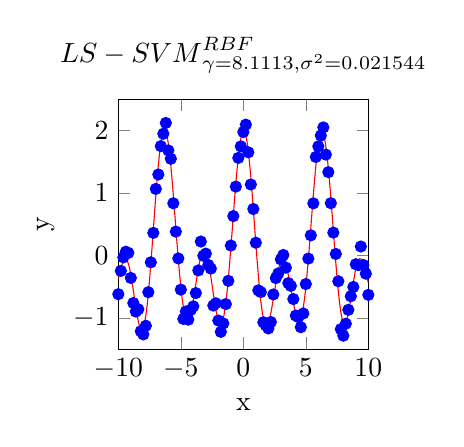
\begin{tikzpicture}

\begin{axis}[%
width=1.25in,
height=1.25in,
scale only axis,
xmin=-10,
xmax=10,
xlabel={x},
ymin=-1.5,
ymax=2.5,
ylabel={y},
title={$\text{LS-SVM}_{\gamma\text{=8.1113,}\sigma{}^\text{2}\text{=0.021544}}^{\text{RBF}}$}
]
\addplot [color=red,solid,forget plot]
  table[row sep=crcr]{%
-10	-0.378155848083547\\
-9.9	-0.294876235938143\\
-9.8	-0.216122205479947\\
-9.7	-0.147876896762239\\
-9.6	-0.0958533699641556\\
-9.5	-0.065043342605781\\
-9.4	-0.0592979764652931\\
-9.3	-0.0809783616834283\\
-9.2	-0.130707121849832\\
-9.1	-0.207243091621335\\
-9	-0.307489519593927\\
-8.9	-0.426634148743443\\
-8.8	-0.558408229639226\\
-8.7	-0.695442210023953\\
-8.6	-0.829689331359161\\
-8.5	-0.952885023239864\\
-8.4	-1.05700976735817\\
-8.3	-1.1347256011633\\
-8.2	-1.17976101320801\\
-8.1	-1.18722491088169\\
-8	-1.1538368915467\\
-7.9	-1.0780675861544\\
-7.8	-0.96018886919266\\
-7.7	-0.802238880544155\\
-7.6	-0.607910853023286\\
-7.5	-0.382377564765225\\
-7.4	-0.13206481668019\\
-7.3	0.135612257220494\\
-7.2	0.412536841558149\\
-7.1	0.690190209721806\\
-7	0.959953564980523\\
-6.9	1.21340377490603\\
-6.8	1.4425964183712\\
-6.7	1.64033061897014\\
-6.6	1.80039051577865\\
-6.5	1.91775795867774\\
-6.4	1.98879032430155\\
-6.3	2.0113565857991\\
-6.2	1.98492436370741\\
-6.1	1.91059104569894\\
-6	1.7910534839738\\
-5.9	1.63051336157977\\
-5.8	1.43451892897771\\
-5.7	1.20974808656245\\
-5.6	0.963742189612541\\
-5.5	0.704603859930663\\
-5.4	0.44067491704934\\
-5.3	0.180211850852144\\
-5.2	-0.0689241602108382\\
-5.1	-0.299547754445033\\
-5	-0.505388873190403\\
-4.9	-0.681283838984376\\
-4.8	-0.823314897917623\\
-4.7	-0.928898825775779\\
-4.6	-0.996827884395797\\
-4.5	-1.02726778403292\\
-4.4	-1.02171735999765\\
-4.3	-0.982933678397346\\
-4.2	-0.914824726648321\\
-4.1	-0.822310305536334\\
-4	-0.711150788793284\\
-3.9	-0.587743483440506\\
-3.8	-0.458887611334805\\
-3.7	-0.331521370033481\\
-3.6	-0.212437791196766\\
-3.5	-0.107989674853166\\
-3.4	-0.0237971226056478\\
-3.3	0.0355264696830814\\
-3.2	0.0666131305368795\\
-3.1	0.067527568285264\\
-3	0.037889080832013\\
-2.9	-0.0210820461907696\\
-2.8	-0.106599067349452\\
-2.7	-0.214424350155148\\
-2.6	-0.339060784151469\\
-2.5	-0.474008925856841\\
-2.4	-0.612075697524962\\
-2.3	-0.745717450838724\\
-2.2	-0.867398429866311\\
-2.1	-0.969945182007542\\
-2	-1.04687825474257\\
-1.9	-1.09270449604647\\
-1.8	-1.10315629752684\\
-1.7	-1.07536796038565\\
-1.6	-1.00798372814477\\
-1.5	-0.901196549991163\\
-1.4	-0.756720902216105\\
-1.3	-0.577706588810396\\
-1.2	-0.368603010833183\\
-1.1	-0.134984706147812\\
-1	0.116651037628226\\
-0.9	0.379104852812625\\
-0.799999999999999	0.644706573224734\\
-0.699999999999999	0.905551757004319\\
-0.6	1.15374016324667\\
-0.5	1.38161426804077\\
-0.399999999999999	1.58199622928933\\
-0.299999999999999	1.74842087713643\\
-0.199999999999999	1.87536047567285\\
-0.0999999999999996	1.95843457253841\\
0	1.9945957951916\\
0.0999999999999996	1.98228059037254\\
0.199999999999999	1.92151318818227\\
0.299999999999999	1.81395186710705\\
0.399999999999999	1.6628689972473\\
0.5	1.47306015170144\\
0.6	1.25068235225715\\
0.699999999999999	1.00302664067485\\
0.799999999999999	0.738234979177406\\
0.9	0.464975398555039\\
1	0.19209192381836\\
1.1	-0.0717530526508091\\
1.2	-0.318426538420568\\
1.3	-0.540646824919553\\
1.4	-0.73226560595447\\
1.5	-0.888498959718327\\
1.6	-1.00609840016916\\
1.7	-1.08345568420302\\
1.8	-1.12063743616203\\
1.9	-1.11934803268286\\
2	-1.08282174273582\\
2.1	-1.0156479716616\\
2.2	-0.923536636461624\\
2.3	-0.813034067688702\\
2.4	-0.691203094567072\\
2.5	-0.565283708979081\\
2.6	-0.442352467372367\\
2.7	-0.328999187767102\\
2.8	-0.231038303755436\\
2.9	-0.153269452796243\\
3	-0.0992977638493906\\
3.1	-0.0714193604237752\\
3.2	-0.0705724519125292\\
3.3	-0.0963497302985599\\
3.4	-0.147064217728661\\
3.5	-0.219858625081448\\
3.6	-0.310847816643414\\
3.7	-0.415284976460339\\
3.8	-0.527744128613192\\
3.9	-0.642314196059252\\
4	-0.752802153103253\\
4.1	-0.852944462395901\\
4.2	-0.936626487620834\\
4.3	-0.998108779872837\\
4.4	-1.03225715920071\\
4.5	-1.03477070694114\\
4.6	-1.00239868198467\\
4.7	-0.933134593399615\\
4.8	-0.826373803915961\\
4.9	-0.683020590901011\\
5	-0.50553185119428\\
5.1	-0.297887664656759\\
5.2	-0.0654835394487272\\
5.3	0.185055070977024\\
5.4	0.446129068930357\\
5.5	0.709479767658797\\
5.6	0.966542396608503\\
5.7	1.20881710445227\\
5.8	1.42823396519454\\
5.9	1.61748932296474\\
6	1.77033397543138\\
6.1	1.88179882980166\\
6.2	1.94835010653516\\
6.3	1.96797303199366\\
6.4	1.94018927507218\\
6.5	1.86601822733625\\
6.6	1.74789490548876\\
6.7	1.58955743151702\\
6.8	1.39591482366046\\
6.9	1.17290176319979\\
7	0.927322011308792\\
7.1	0.666677374720198\\
7.2	0.398975702504972\\
7.3	0.132510265317376\\
7.4	-0.124395461506011\\
7.5	-0.363679137594506\\
7.6	-0.577861891395248\\
7.7	-0.760388718502137\\
7.8	-0.905966427432029\\
7.9	-1.01087266836014\\
8	-1.07320651161869\\
8.1	-1.09305168336255\\
8.2	-1.07252818913541\\
8.3	-1.01571632761261\\
8.4	-0.928448126531717\\
8.5	-0.817973716505258\\
8.6	-0.692522577921945\\
8.7	-0.560790441156105\\
8.8	-0.431390593964865\\
8.9	-0.312312528703424\\
9	-0.210430791627665\\
9.1	-0.131102619710374\\
9.2	-0.0778849716734599\\
9.3	-0.0523907623848497\\
9.4	-0.054291639277566\\
9.5	-0.0814617731758166\\
9.6	-0.130245148220669\\
9.7	-0.195818872156336\\
9.8	-0.272617996960495\\
9.9	-0.354783825863167\\
10	-0.436597895179934\\
};
\addplot [color=blue,only marks,mark=*,mark options={solid},forget plot]
  table[row sep=crcr]{%
-10	-0.619595049893259\\
-9.8	-0.247437337833684\\
-9.6	-0.0306624145407526\\
-9.4	0.0595016992990417\\
-9.2	0.0405503353753764\\
-9	-0.359577760153356\\
-8.8	-0.761497412492202\\
-8.6	-0.897663190767661\\
-8.4	-0.860637115262312\\
-8.2	-1.2126167956593\\
-8	-1.26313692928078\\
-7.8	-1.12516839132702\\
-7.6	-0.588065125145126\\
-7.4	-0.109694576560566\\
-7.2	0.361280183367072\\
-7	1.0646759786683\\
-6.8	1.29538129968242\\
-6.6	1.74884224001031\\
-6.4	1.94683351065395\\
-6.2	2.11982365358625\\
-6	1.68022816856692\\
-5.8	1.54627677608122\\
-5.6	0.834565398848264\\
-5.4	0.381366445534563\\
-5.2	-0.0478095833588603\\
-5	-0.546903359444873\\
-4.8	-1.01522643475883\\
-4.6	-0.897166537197328\\
-4.4	-1.02680658292176\\
-4.2	-0.871089932079635\\
-4	-0.814155649020787\\
-3.8	-0.60175571130384\\
-3.6	-0.238907143455007\\
-3.4	0.222208137340781\\
-3.2	-0.00492514934068313\\
-3	0.0292466251038767\\
-2.8	-0.152773332407692\\
-2.6	-0.210247299070627\\
-2.4	-0.801924853922079\\
-2.2	-0.765333121147812\\
-2	-1.04175373212827\\
-1.8	-1.22268061922734\\
-1.6	-1.08813837606648\\
-1.4	-0.778398776369186\\
-1.2	-0.406010477529214\\
-1	0.158410672742104\\
-0.799999999999999	0.629656009659678\\
-0.6	1.1012539129474\\
-0.399999999999999	1.56095744357927\\
-0.199999999999999	1.74538482106182\\
0	1.97514838527262\\
0.199999999999999	2.09333728242314\\
0.399999999999999	1.65001281210317\\
0.6	1.13516770216898\\
0.799999999999999	0.742729092315044\\
1	0.203344072966865\\
1.2	-0.558470765447578\\
1.4	-0.586110482986666\\
1.6	-1.06883931097022\\
1.8	-1.11741980461136\\
2	-1.16758084046331\\
2.2	-1.06511621288888\\
2.4	-0.623929796601062\\
2.6	-0.362230376187371\\
2.8	-0.286628861691811\\
3	-0.0622448540645585\\
3.2	0.00790495738628174\\
3.4	-0.194949615007405\\
3.6	-0.442522817019591\\
3.8	-0.486757328807435\\
4	-0.69787996654234\\
4.2	-0.962269330093291\\
4.4	-0.985769144108822\\
4.6	-1.14773117213016\\
4.8	-0.92842012618687\\
5	-0.457544358332057\\
5.2	-0.0501283831683725\\
5.4	0.321923931056346\\
5.6	0.833778247649155\\
5.8	1.5757751546434\\
6	1.74494490112986\\
6.2	1.91809847491895\\
6.4	2.04847928009022\\
6.6	1.61361768813205\\
6.8	1.33288010477131\\
7	0.836064061458198\\
7.2	0.365373991683923\\
7.4	0.0243115018755421\\
7.6	-0.412557611585228\\
7.8	-1.17965097458037\\
8	-1.28369946344995\\
8.2	-1.09154240409875\\
8.4	-0.869970337849687\\
8.6	-0.652727819002938\\
8.8	-0.504839095267686\\
9	-0.140625208970404\\
9.2	-0.155007196552229\\
9.4	0.142883162331669\\
9.6	-0.152697183256788\\
9.8	-0.291450155475497\\
10	-0.630494381710576\\
};
\end{axis}
\end{tikzpicture}%
\end{document}
% This file was created by matlab2tikz.
% Minimal pgfplots version: 1.3
%
%The latest updates can be retrieved from
%  http://www.mathworks.com/matlabcentral/fileexchange/22022-matlab2tikz
%where you can also make suggestions and rate matlab2tikz.
%
\documentclass[tikz]{standalone}
\usepackage{pgfplots}
\usepackage{grffile}
\pgfplotsset{compat=newest}
\usetikzlibrary{plotmarks}
\usepackage{amsmath}

\begin{document}
\definecolor{mycolor1}{rgb}{0.00000,0.44700,0.74100}%
\definecolor{mycolor2}{rgb}{0.85000,0.32500,0.09800}%
%
\begin{tikzpicture}

\begin{axis}[%
width=1.25in,
height=1.25in,
scale only axis,
xmin=-10,
xmax=10,
ymin=-1.5,
ymax=2.5,
xlabel={x},
ylabel={y},
legend style={legend cell align=left,align=left,draw=white!15!black}
]
\addplot [color=mycolor1,only marks,mark=*,mark options={solid}]
  table[row sep=crcr]{%
-9.9	-0.446457785387605\\
-9.7	0.0615741857353768\\
-9.5	-0.0899003134505097\\
-9.3	0.00653549107191894\\
-9.1	-0.233751653584901\\
-8.9	-0.291859160079753\\
-8.7	-0.613731475283965\\
-8.5	-1.03528169296305\\
-8.3	-0.9642330834576\\
-8.1	-1.27978596939285\\
-7.9	-0.986978063124592\\
-7.7	-0.941541670603769\\
-7.5	-0.424284871548671\\
-7.3	0.0024000252430941\\
-7.1	0.612256274995885\\
-6.9	1.10201532421862\\
-6.7	1.60211115914485\\
-6.5	1.76220978074123\\
-6.3	1.99979524181867\\
-6.1	1.79034879732083\\
-5.9	1.44403094330746\\
-5.7	1.29383877713738\\
-5.5	0.613830121265493\\
-5.3	0.100331531211364\\
-5.1	-0.325372368531793\\
-4.9	-0.64567925384688\\
-4.7	-0.96024547762059\\
-4.5	-1.07928199677673\\
-4.3	-0.972498020860962\\
-4.1	-1.02965915981306\\
-3.9	-0.755152776972108\\
-3.7	-0.589677281173566\\
-3.5	-0.166490277986134\\
-3.3	0.0236256253118752\\
-3.1	-0.22676123328907\\
-2.9	-0.23110988817597\\
-2.7	-0.200813017281912\\
-2.5	-0.491113134760776\\
-2.3	-0.84073572657711\\
-2.1	-0.985056993540881\\
-1.9	-1.05132963955875\\
-1.7	-1.15426680135552\\
-1.5	-0.779866365644407\\
-1.3	-0.688580620762527\\
-1.1	-0.0433129495232868\\
-0.9	0.508987303868705\\
-0.699999999999999	0.697600560057975\\
-0.5	1.42603297588922\\
-0.299999999999999	1.89054346075414\\
-0.0999999999999996	1.99857339590222\\
0.0999999999999996	1.70788159322484\\
0.299999999999999	1.6759300758617\\
0.5	1.49638851300071\\
0.699999999999999	1.04119258285231\\
0.9	0.301598925511327\\
1.1	-0.159278370503842\\
1.3	-0.529632069442699\\
1.5	-0.869771393788035\\
1.7	-1.20941576364803\\
1.9	-1.18707415269971\\
2.1	-1.05532322902962\\
2.3	-0.797889105745886\\
2.5	-0.498836517243156\\
2.7	-0.370696460770287\\
2.9	-0.212410851613561\\
3.1	-0.0759893540469849\\
3.3	0.202379146677431\\
3.5	-0.15504532673161\\
3.7	-0.455920196582363\\
3.9	-0.883007950496145\\
4.1	-0.798073602984103\\
4.3	-1.15799842570728\\
4.5	-1.10879202963167\\
4.7	-1.14475761549896\\
4.9	-0.718500284867997\\
5.1	-0.399271702450803\\
5.3	0.0633190838576606\\
5.5	0.828518914985831\\
5.7	1.31722910868865\\
5.9	1.60141103275897\\
6.1	1.7846292176811\\
6.3	2.07597483058294\\
6.5	1.86948734102912\\
6.7	1.5439487097687\\
6.9	1.0778203170723\\
7.1	0.804338148231601\\
7.3	0.0295045907637691\\
7.5	-0.390997298935905\\
7.7	-0.677198469150053\\
7.9	-1.21318786763014\\
8.1	-1.22754939070245\\
8.3	-1.03150807115426\\
8.5	-0.948758708294413\\
8.7	-0.612207588633159\\
8.9	-0.342665934347301\\
9.1	-0.184215026650319\\
9.3	-0.0609189088953476\\
9.5	0.0628781633101973\\
9.7	-0.0694799394785849\\
9.9	-0.153493005615711\\
};

\addplot [color=mycolor2,only marks,mark=+,mark options={solid}]
  table[row sep=crcr]{%
-9.9	-0.294876235938143\\
-9.7	-0.147876896762239\\
-9.5	-0.065043342605781\\
-9.3	-0.0809783616834283\\
-9.1	-0.207243091621335\\
-8.9	-0.426634148743443\\
-8.7	-0.695442210023953\\
-8.5	-0.952885023239864\\
-8.3	-1.1347256011633\\
-8.1	-1.18722491088169\\
-7.9	-1.0780675861544\\
-7.7	-0.802238880544155\\
-7.5	-0.382377564765225\\
-7.3	0.135612257220494\\
-7.1	0.690190209721806\\
-6.9	1.21340377490603\\
-6.7	1.64033061897014\\
-6.5	1.91775795867774\\
-6.3	2.0113565857991\\
-6.1	1.91059104569894\\
-5.9	1.63051336157977\\
-5.7	1.20974808656245\\
-5.5	0.704603859930663\\
-5.3	0.180211850852144\\
-5.1	-0.299547754445033\\
-4.9	-0.681283838984376\\
-4.7	-0.928898825775779\\
-4.5	-1.02726778403292\\
-4.3	-0.982933678397346\\
-4.1	-0.822310305536334\\
-3.9	-0.587743483440506\\
-3.7	-0.331521370033481\\
-3.5	-0.107989674853166\\
-3.3	0.0355264696830814\\
-3.1	0.067527568285264\\
-2.9	-0.0210820461907696\\
-2.7	-0.214424350155148\\
-2.5	-0.474008925856841\\
-2.3	-0.745717450838724\\
-2.1	-0.969945182007542\\
-1.9	-1.09270449604647\\
-1.7	-1.07536796038565\\
-1.5	-0.901196549991163\\
-1.3	-0.577706588810396\\
-1.1	-0.134984706147812\\
-0.9	0.379104852812625\\
-0.699999999999999	0.905551757004319\\
-0.5	1.38161426804077\\
-0.299999999999999	1.74842087713643\\
-0.0999999999999996	1.95843457253841\\
0.0999999999999996	1.98228059037254\\
0.299999999999999	1.81395186710705\\
0.5	1.47306015170144\\
0.699999999999999	1.00302664067485\\
0.9	0.464975398555039\\
1.1	-0.0717530526508091\\
1.3	-0.540646824919553\\
1.5	-0.888498959718327\\
1.7	-1.08345568420302\\
1.9	-1.11934803268286\\
2.1	-1.0156479716616\\
2.3	-0.813034067688702\\
2.5	-0.565283708979081\\
2.7	-0.328999187767102\\
2.9	-0.153269452796243\\
3.1	-0.0714193604237752\\
3.3	-0.0963497302985599\\
3.5	-0.219858625081448\\
3.7	-0.415284976460339\\
3.9	-0.642314196059252\\
4.1	-0.852944462395901\\
4.3	-0.998108779872837\\
4.5	-1.03477070694114\\
4.7	-0.933134593399615\\
4.9	-0.683020590901011\\
5.1	-0.297887664656759\\
5.3	0.185055070977024\\
5.5	0.709479767658797\\
5.7	1.20881710445227\\
5.9	1.61748932296474\\
6.1	1.88179882980166\\
6.3	1.96797303199366\\
6.5	1.86601822733625\\
6.7	1.58955743151702\\
6.9	1.17290176319979\\
7.1	0.666677374720198\\
7.3	0.132510265317376\\
7.5	-0.363679137594506\\
7.7	-0.760388718502137\\
7.9	-1.01087266836014\\
8.1	-1.09305168336255\\
8.3	-1.01571632761261\\
8.5	-0.817973716505258\\
8.7	-0.560790441156105\\
8.9	-0.312312528703424\\
9.1	-0.131102619710374\\
9.3	-0.0523907623848497\\
9.5	-0.0814617731758166\\
9.7	-0.195818872156336\\
9.9	-0.354783825863167\\
};

\end{axis}
\end{tikzpicture}%
\end{document}
% This file was created by matlab2tikz.
% Minimal pgfplots version: 1.3
%
%The latest updates can be retrieved from
%  http://www.mathworks.com/matlabcentral/fileexchange/22022-matlab2tikz
%where you can also make suggestions and rate matlab2tikz.
%
\documentclass[tikz]{standalone}
\usepackage{pgfplots}
\usepackage{grffile}
\pgfplotsset{compat=newest}
\usetikzlibrary{plotmarks}
\usepackage{amsmath}

\begin{document}
\begin{tikzpicture}

\begin{axis}[%
width=1.25in,
height=1.25in,
scale only axis,
xmin=-5,
xmax=0,
xlabel={$\sigma^2$},
xmajorgrids,
ymin=0,
ymax=10,
ylabel={$\gamma$},
ymajorgrids,
zmin=0,
zmax=10,
zmajorgrids,
view={90}{90},
axis x line*=bottom,
axis y line*=left,
axis z line*=left
]

\addplot3[%
surf,
shader=flat,
colormap={mymap}{[1pt] rgb(0pt)=(0.2081,0.1663,0.5292); rgb(1pt)=(0.211624,0.189781,0.577676); rgb(2pt)=(0.212252,0.213771,0.626971); rgb(3pt)=(0.2081,0.2386,0.677086); rgb(4pt)=(0.195905,0.264457,0.7279); rgb(5pt)=(0.170729,0.291938,0.779248); rgb(6pt)=(0.125271,0.324243,0.830271); rgb(7pt)=(0.0591333,0.359833,0.868333); rgb(8pt)=(0.0116952,0.38751,0.881957); rgb(9pt)=(0.00595714,0.408614,0.882843); rgb(10pt)=(0.0165143,0.4266,0.878633); rgb(11pt)=(0.0328524,0.443043,0.871957); rgb(12pt)=(0.0498143,0.458571,0.864057); rgb(13pt)=(0.0629333,0.47369,0.855438); rgb(14pt)=(0.0722667,0.488667,0.8467); rgb(15pt)=(0.0779429,0.503986,0.838371); rgb(16pt)=(0.0793476,0.520024,0.831181); rgb(17pt)=(0.0749429,0.537543,0.826271); rgb(18pt)=(0.0640571,0.556986,0.823957); rgb(19pt)=(0.0487714,0.577224,0.822829); rgb(20pt)=(0.0343429,0.596581,0.819852); rgb(21pt)=(0.0265,0.6137,0.8135); rgb(22pt)=(0.0238905,0.628662,0.803762); rgb(23pt)=(0.0230905,0.641786,0.791267); rgb(24pt)=(0.0227714,0.653486,0.776757); rgb(25pt)=(0.0266619,0.664195,0.760719); rgb(26pt)=(0.0383714,0.674271,0.743552); rgb(27pt)=(0.0589714,0.683757,0.725386); rgb(28pt)=(0.0843,0.692833,0.706167); rgb(29pt)=(0.113295,0.7015,0.685857); rgb(30pt)=(0.145271,0.709757,0.664629); rgb(31pt)=(0.180133,0.717657,0.642433); rgb(32pt)=(0.217829,0.725043,0.619262); rgb(33pt)=(0.258643,0.731714,0.595429); rgb(34pt)=(0.302171,0.737605,0.571186); rgb(35pt)=(0.348167,0.742433,0.547267); rgb(36pt)=(0.395257,0.7459,0.524443); rgb(37pt)=(0.44201,0.748081,0.503314); rgb(38pt)=(0.487124,0.749062,0.483976); rgb(39pt)=(0.530029,0.749114,0.466114); rgb(40pt)=(0.570857,0.748519,0.44939); rgb(41pt)=(0.609852,0.747314,0.433686); rgb(42pt)=(0.6473,0.7456,0.4188); rgb(43pt)=(0.683419,0.743476,0.404433); rgb(44pt)=(0.71841,0.741133,0.390476); rgb(45pt)=(0.752486,0.7384,0.376814); rgb(46pt)=(0.785843,0.735567,0.363271); rgb(47pt)=(0.818505,0.732733,0.34979); rgb(48pt)=(0.850657,0.7299,0.336029); rgb(49pt)=(0.882433,0.727433,0.3217); rgb(50pt)=(0.913933,0.725786,0.306276); rgb(51pt)=(0.944957,0.726114,0.288643); rgb(52pt)=(0.973895,0.731395,0.266648); rgb(53pt)=(0.993771,0.745457,0.240348); rgb(54pt)=(0.999043,0.765314,0.216414); rgb(55pt)=(0.995533,0.786057,0.196652); rgb(56pt)=(0.988,0.8066,0.179367); rgb(57pt)=(0.978857,0.827143,0.163314); rgb(58pt)=(0.9697,0.848138,0.147452); rgb(59pt)=(0.962586,0.870514,0.1309); rgb(60pt)=(0.958871,0.8949,0.113243); rgb(61pt)=(0.959824,0.921833,0.0948381); rgb(62pt)=(0.9661,0.951443,0.0755333); rgb(63pt)=(0.9763,0.9831,0.0538)},
mesh/rows=100]
table[row sep=crcr,header=false] {%
%
-5	0	9.71142221677984\\
-5	0.101010101010101	9.71140389779787\\
-5	0.202020202020202	9.71133157748906\\
-5	0.303030303030303	9.71108866364165\\
-5	0.404040404040404	9.71038231696047\\
-5	0.505050505050505	9.70857639673274\\
-5	0.606060606060606	9.70445997701801\\
-5	0.707070707070707	9.69599033644247\\
-5	0.808080808080808	9.68008498106293\\
-5	0.909090909090909	9.65255230147744\\
-5	1.01010101010101	9.60823099716993\\
-5	1.11111111111111	9.54135739289275\\
-5	1.21212121212121	9.44611626222461\\
-5	1.31313131313131	9.31727946697319\\
-5	1.41414141414141	9.15081579818331\\
-5	1.51515151515152	8.94436985684349\\
-5	1.61616161616162	8.69755000378289\\
-5	1.71717171717172	8.41201953179298\\
-5	1.81818181818182	8.0914319996519\\
-5	1.91919191919192	7.74127308928682\\
-5	2.02020202020202	7.36865697285339\\
-5	2.12121212121212	6.98207929813651\\
-5	2.22222222222222	6.59107386107618\\
-5	2.32323232323232	6.20569089073058\\
-5	2.42424242424242	5.83574370568315\\
-5	2.52525252525253	5.48986433431911\\
-5	2.62626262626263	5.17453335022118\\
-5	2.72727272727273	4.89333662120591\\
-5	2.82828282828283	4.64668763180221\\
-5	2.92929292929293	4.43212530463919\\
-5	3.03030303030303	4.24510923332891\\
-5	3.13131313131313	4.08007813894372\\
-5	3.23232323232323	3.93148179992769\\
-5	3.33333333333333	3.79455148521732\\
-5	3.43434343434343	3.66569731720236\\
-5	3.53535353535354	3.54255252096777\\
-5	3.63636363636364	3.42377535273262\\
-5	3.73737373737374	3.30874825928866\\
-5	3.83838383838384	3.19728824561706\\
-5	3.93939393939394	3.08942972027933\\
-5	4.04040404040404	2.98529117204018\\
-5	4.14141414141414	2.88500760942979\\
-5	4.24242424242424	2.7887029600321\\
-5	4.34343434343434	2.69648196820019\\
-5	4.44444444444444	2.60843039263769\\
-5	4.54545454545455	2.52461997905935\\
-5	4.64646464646465	2.44511830184894\\
-5	4.74747474747475	2.37000278952208\\
-5	4.84848484848485	2.29937513088621\\
-5	4.94949494949495	2.23337054344156\\
-5	5.05050505050505	2.17215862952682\\
-5	5.15151515151515	2.11593761748802\\
-5	5.25252525252525	2.0649278213709\\
-5	5.35353535353535	2.01937036709782\\
-5	5.45454545454545	1.97953458705286\\
-5	5.55555555555556	1.94573519074472\\
-5	5.65656565656566	1.91835994277943\\
-5	5.75757575757576	1.8979088670444\\
-5	5.85858585858586	1.88504540661013\\
-5	5.95959595959596	1.88065819624512\\
-5	6.06060606060606	1.88592995845182\\
-5	6.16161616161616	1.90241064246018\\
-5	6.26262626262626	1.9320985452317\\
-5	6.36363636363636	1.97754138993487\\
-5	6.46464646464646	2.04196706625944\\
-5	6.56565656565657	2.1294342344993\\
-5	6.66666666666667	2.24496291455581\\
-5	6.76767676767677	2.39457352575721\\
-5	6.86868686868687	2.58512511060784\\
-5	6.96969696969697	2.82378869281159\\
-5	7.07070707070707	3.11693714371589\\
-5	7.17171717171717	3.46825403441113\\
-5	7.27272727272727	3.87609364592065\\
-5	7.37373737373737	4.33068823175355\\
-5	7.47474747474747	4.81258912661282\\
-5	7.57575757575758	5.29411277134777\\
-5	7.67676767676768	5.74466615932254\\
-5	7.77777777777778	6.1386580399485\\
-5	7.87878787878788	6.46268248672824\\
-5	7.97979797979798	6.71848722691886\\
-5	8.08080808080808	6.92046177476854\\
-5	8.18181818181818	7.08967133544705\\
-5	8.28282828282828	7.24803947536821\\
-5	8.38383838383838	7.41463350493836\\
-5	8.48484848484848	7.60328127105507\\
-5	8.58585858585859	7.82033916154883\\
-5	8.68686868686869	8.06332431777104\\
-5	8.78787878787879	8.3220094751847\\
-5	8.88888888888889	8.58185903084134\\
-5	8.98989898989899	8.82781708099047\\
-5	9.09090909090909	9.04692345740679\\
-5	9.19191919191919	9.22989559098724\\
-5	9.29292929292929	9.3722784283822\\
-5	9.39393939393939	9.47495304520139\\
-5	9.49494949494949	9.54339029446297\\
-5	9.5959595959596	9.58572657183269\\
-5	9.6969696969697	9.61054080474783\\
-5	9.7979797979798	9.62520371347509\\
-5	9.8989898989899	9.63509098847121\\
-5	10	9.64348641937173\\
-4.94949494949495	0	9.71142167926959\\
-4.94949494949495	0.101010101010101	9.71140123948528\\
-4.94949494949495	0.202020202020202	9.71132054660067\\
-4.94949494949495	0.303030303030303	9.71104951044657\\
-4.94949494949495	0.404040404040404	9.71026138959856\\
-4.94949494949495	0.505050505050505	9.70824639750565\\
-4.94949494949495	0.606060606060606	9.70365342186232\\
-4.94949494949495	0.707070707070707	9.69420326857134\\
-4.94949494949495	0.808080808080808	9.67645663259656\\
-4.94949494949495	0.909090909090909	9.64573679145825\\
-4.94949494949495	1.01010101010101	9.59628530601474\\
-4.94949494949495	1.11111111111111	9.52167210570779\\
-4.94949494949495	1.21212121212121	9.41541047427978\\
-4.94949494949495	1.31313131313131	9.27167022464262\\
-4.94949494949495	1.41414141414141	9.08595911475644\\
-4.94949494949495	1.51515151515152	8.85565901346967\\
-4.94949494949495	1.61616161616162	8.58035107999663\\
-4.94949494949495	1.71717171717172	8.26192551433383\\
-4.94949494949495	1.81818181818182	7.90452410458374\\
-4.94949494949495	1.91919191919192	7.51438654115999\\
-4.94949494949495	2.02020202020202	7.0996516222492\\
-4.94949494949495	2.12121212121212	6.67010710495475\\
-4.94949494949495	2.22222222222222	6.2368144501488\\
-4.94949494949495	2.32323232323232	5.81150061203663\\
-4.94949494949495	2.42424242424242	5.40564862921429\\
-4.94949494949495	2.52525252525253	5.0293408896816\\
-4.94949494949495	2.62626262626263	4.69006926222821\\
-4.94949494949495	2.72727272727273	4.39183586154036\\
-4.94949494949495	2.82828282828283	4.13484309383091\\
-4.94949494949495	2.92929292929293	3.91589759875969\\
-4.94949494949495	3.03030303030303	3.72940929941481\\
-4.94949494949495	3.13131313131313	3.56867815139841\\
-4.94949494949495	3.23232323232323	3.42711129047998\\
-4.94949494949495	3.33333333333333	3.29910031912854\\
-4.94949494949495	3.43434343434343	3.18044735504394\\
-4.94949494949495	3.53535353535354	3.06838260582747\\
-4.94949494949495	3.63636363636364	2.96131347086355\\
-4.94949494949495	3.73737373737374	2.85846859127728\\
-4.94949494949495	3.83838383838384	2.75956424499123\\
-4.94949494949495	3.93939393939394	2.66455798115544\\
-4.94949494949495	4.04040404040404	2.57349861728354\\
-4.94949494949495	4.14141414141414	2.48645051966548\\
-4.94949494949495	4.24242424242424	2.40346267272872\\
-4.94949494949495	4.34343434343434	2.32455912594137\\
-4.94949494949495	4.44444444444444	2.24973781869955\\
-4.94949494949495	4.54545454545455	2.17897444802103\\
-4.94949494949495	4.64646464646465	2.11223348696236\\
-4.94949494949495	4.74747474747475	2.04948735615473\\
-4.94949494949495	4.84848484848485	1.99073875889208\\
-4.94949494949495	4.94949494949495	1.93603652701466\\
-4.94949494949495	5.05050505050505	1.88547768913874\\
-4.94949494949495	5.15151515151515	1.83919701420085\\
-4.94949494949495	5.25252525252525	1.79735295563202\\
-4.94949494949495	5.35353535353535	1.76011955550373\\
-4.94949494949495	5.45454545454545	1.72768850749617\\
-4.94949494949495	5.55555555555556	1.70028095650879\\
-4.94949494949495	5.65656565656566	1.67816897424019\\
-4.94949494949495	5.75757575757576	1.66170938774762\\
-4.94949494949495	5.85858585858586	1.6513935043361\\
-4.94949494949495	5.95959595959596	1.64791398445157\\
-4.94949494949495	6.06060606060606	1.65224472704423\\
-4.94949494949495	6.16161616161616	1.66572511709204\\
-4.94949494949495	6.26262626262626	1.69014602761138\\
-4.94949494949495	6.36363636363636	1.72785240715437\\
-4.94949494949495	6.46464646464646	1.78188735013213\\
-4.94949494949495	6.56565656565657	1.85618624370098\\
-4.94949494949495	6.66666666666667	1.95579174725998\\
-4.94949494949495	6.76767676767677	2.08702104609988\\
-4.94949494949495	6.86868686868687	2.25747909494098\\
-4.94949494949495	6.96969696969697	2.47575095474901\\
-4.94949494949495	7.07070707070707	2.75051357026197\\
-4.94949494949495	7.17171717171717	3.08874494239786\\
-4.94949494949495	7.27272727272727	3.49282919494749\\
-4.94949494949495	7.37373737373737	3.95688315816791\\
-4.94949494949495	7.47474747474747	4.46366456236852\\
-4.94949494949495	7.57575757575758	4.98441392518124\\
-4.94949494949495	7.67676767676768	5.4835770422405\\
-4.94949494949495	7.77777777777778	5.92784674631657\\
-4.94949494949495	7.87878787878788	6.29588498128486\\
-4.94949494949495	7.97979797979798	6.58395937428513\\
-4.94949494949495	8.08080808080808	6.80473062566524\\
-4.94949494949495	8.18181818181818	6.98061837615216\\
-4.94949494949495	8.28282828282828	7.13635993918139\\
-4.94949494949495	8.38383838383838	7.29433669600206\\
-4.94949494949495	8.48484848484848	7.47221753174323\\
-4.94949494949495	8.58585858585859	7.68055240248904\\
-4.94949494949495	8.68686868686869	7.92025187553388\\
-4.94949494949495	8.78787878787879	8.18247699547346\\
-4.94949494949495	8.88888888888889	8.45213493813682\\
-4.94949494949495	8.98989898989899	8.71276515824471\\
-4.94949494949495	9.09090909090909	8.94994866268236\\
-4.94949494949495	9.19191919191919	9.15280818127921\\
-4.94949494949495	9.29292929292929	9.31489132876324\\
-4.94949494949495	9.39393939393939	9.43497492753353\\
-4.94949494949495	9.49494949494949	9.51702075432333\\
-4.94949494949495	9.5959595959596	9.56869339834603\\
-4.94949494949495	9.6969696969697	9.59902583698428\\
-4.94949494949495	9.7979797979798	9.61634990417677\\
-4.94949494949495	9.8989898989899	9.6271213478953\\
-4.94949494949495	10	9.63558666025153\\
-4.8989898989899	0	9.71142115597714\\
-4.8989898989899	0.101010101010101	9.7113986514883\\
-4.8989898989899	0.202020202020202	9.71130980749288\\
-4.8989898989899	0.303030303030303	9.7110113929039\\
-4.8989898989899	0.404040404040404	9.7101436609396\\
-4.8989898989899	0.505050505050505	9.70792512736293\\
-4.8989898989899	0.606060606060606	9.702868202291\\
-4.8989898989899	0.707070707070707	9.6924634768283\\
-4.8989898989899	0.808080808080808	9.67292428327859\\
-4.8989898989899	0.909090909090909	9.63910164875787\\
-4.8989898989899	1.01010101010101	9.58465587001585\\
-4.8989898989899	1.11111111111111	9.50250828914412\\
-4.8989898989899	1.21212121212121	9.38551883486359\\
-4.8989898989899	1.31313131313131	9.22727191171258\\
-4.8989898989899	1.41414141414141	9.02282775994852\\
-4.8989898989899	1.51515151515152	8.76931489581012\\
-4.8989898989899	1.61616161616162	8.46629256379988\\
-4.8989898989899	1.71717171717172	8.11588060542613\\
-4.8989898989899	1.81818181818182	7.72271264876739\\
-4.8989898989899	1.91919191919192	7.29379229846441\\
-4.8989898989899	2.02020202020202	6.83830594222351\\
-4.8989898989899	2.12121212121212	6.36737566103727\\
-4.8989898989899	2.22222222222222	5.89365428089877\\
-4.8989898989899	2.32323232323232	5.43062472244378\\
-4.8989898989899	2.42424242424242	4.99151731014569\\
-4.8989898989899	2.52525252525253	4.58791332947794\\
-4.8989898989899	2.62626262626263	4.22830603995841\\
-4.8989898989899	2.72727272727273	3.91702817487881\\
-4.8989898989899	2.82828282828283	3.65391775839005\\
-4.8989898989899	2.92929292929293	3.43486286096809\\
-4.8989898989899	3.03030303030303	3.25305057514249\\
-4.8989898989899	3.13131313131313	3.10051718135014\\
-4.8989898989899	3.23232323232323	2.9695612412471\\
-4.8989898989899	3.33333333333333	2.85371676368859\\
-4.8989898989899	3.43434343434343	2.74818759234587\\
-4.8989898989899	3.53535353535354	2.64982009826396\\
-4.8989898989899	3.63636363636364	2.55678877897035\\
-4.8989898989899	3.73737373737374	2.46818186836429\\
-4.8989898989899	3.83838383838384	2.38362482822519\\
-4.8989898989899	3.93939393939394	2.30300704929493\\
-4.8989898989899	4.04040404040404	2.22631673562568\\
-4.8989898989899	4.14141414141414	2.15355765304934\\
-4.8989898989899	4.24242424242424	2.08471521981004\\
-4.8989898989899	4.34343434343434	2.01974571934483\\
-4.8989898989899	4.44444444444444	1.95857301061678\\
-4.8989898989899	4.54545454545455	1.90108908512702\\
-4.8989898989899	4.64646464646465	1.84716386045173\\
-4.8989898989899	4.74747474747475	1.79666936362681\\
-4.8989898989899	4.84848484848485	1.74951327798803\\
-4.8989898989899	4.94949494949495	1.70566621645429\\
-4.8989898989899	5.05050505050505	1.66516798807196\\
-4.8989898989899	5.15151515151515	1.62811184133638\\
-4.8989898989899	5.25252525252525	1.59462031385172\\
-4.8989898989899	5.35353535353535	1.56482886051304\\
-4.8989898989899	5.45454545454545	1.53888330512759\\
-4.8989898989899	5.55555555555556	1.51694685382617\\
-4.8989898989899	5.65656565656566	1.49921279926798\\
-4.8989898989899	5.75757575757576	1.48592661522348\\
-4.8989898989899	5.85858585858586	1.47742596158717\\
-4.8989898989899	5.95959595959596	1.47420601509774\\
-4.8989898989899	6.06060606060606	1.47700964422562\\
-4.8989898989899	6.16161616161616	1.4869284678625\\
-4.8989898989899	6.26262626262626	1.50549845840044\\
-4.8989898989899	6.36363636363636	1.53479816789723\\
-4.8989898989899	6.46464646464646	1.57758845532594\\
-4.8989898989899	6.56565656565657	1.63752982214137\\
-4.8989898989899	6.66666666666667	1.71946908855682\\
-4.8989898989899	6.76767676767677	1.82973256743275\\
-4.8989898989899	6.86868686868687	1.97632218342501\\
-4.8989898989899	6.96969696969697	2.16885711088899\\
-4.8989898989899	7.07070707070707	2.41799105763676\\
-4.8989898989899	7.17171717171717	2.73389516726339\\
-4.8989898989899	7.27272727272727	3.12337584673758\\
-4.8989898989899	7.37373737373737	3.58557189833135\\
-4.8989898989899	7.47474747474747	4.10728706816297\\
-4.8989898989899	7.57575757575758	4.6606579439321\\
-4.8989898989899	7.67676767676768	5.20639059924981\\
-4.8989898989899	7.77777777777778	5.70332643078666\\
-4.8989898989899	7.87878787878788	6.12076055157436\\
-4.8989898989899	7.97979797979798	6.44744585514821\\
-4.8989898989899	8.08080808080808	6.69265650831167\\
-4.8989898989899	8.18181818181818	6.87943820408952\\
-4.8989898989899	8.28282828282828	7.0352240793639\\
-4.8989898989899	8.38383838383838	7.18554953134677\\
-4.8989898989899	8.48484848484848	7.35167936696039\\
-4.8989898989899	8.58585858585859	7.54861433843531\\
-4.8989898989899	8.68686868686869	7.78164870938277\\
-4.8989898989899	8.78787878787879	8.04437786969273\\
-4.8989898989899	8.88888888888889	8.32147098928821\\
-4.8989898989899	8.98989898989899	8.5947628466627\\
-4.8989898989899	9.09090909090909	8.84819782004623\\
-4.8989898989899	9.19191919191919	9.06962906690476\\
-4.8989898989899	9.29292929292929	9.25108799702017\\
-4.8989898989899	9.39393939393939	9.38934931631035\\
-4.8989898989899	9.49494949494949	9.48648273020967\\
-4.8989898989899	9.5959595959596	9.54912439192425\\
-4.8989898989899	9.6969696969697	9.58634459938198\\
-4.8989898989899	9.7979797979798	9.60724548366497\\
-4.8989898989899	9.8989898989899	9.61933660453129\\
-4.8989898989899	10	9.62789871587176\\
-4.84848484848485	0	9.71142065965474\\
-4.84848484848485	0.101010101010101	9.7113961968745\\
-4.84848484848485	0.202020202020202	9.71129962186986\\
-4.84848484848485	0.303030303030303	9.7109752399098\\
-4.84848484848485	0.404040404040404	9.71003199994121\\
-4.84848484848485	0.505050505050505	9.70762041539801\\
-4.84848484848485	0.606060606060606	9.7021234533865\\
-4.84848484848485	0.707070707070707	9.69081335796635\\
-4.84848484848485	0.808080808080808	9.66957401100797\\
-4.84848484848485	0.909090909090909	9.63280855682833\\
-4.84848484848485	1.01010101010101	9.57362605886851\\
-4.84848484848485	1.11111111111111	9.48433286647257\\
-4.84848484848485	1.21212121212121	9.35716957354237\\
-4.84848484848485	1.31313131313131	9.18516602018365\\
-4.84848484848485	1.41414141414141	8.96295925145779\\
-4.84848484848485	1.51515151515152	8.68743983630173\\
-4.84848484848485	1.61616161616162	8.35815070019567\\
-4.84848484848485	1.71717171717172	7.97743810585019\\
-4.84848484848485	1.81818181818182	7.55041856915412\\
-4.84848484848485	1.91919191919192	7.08485004892249\\
-4.84848484848485	2.02020202020202	6.59096298815647\\
-4.84848484848485	2.12121212121212	6.08122305336312\\
-4.84848484848485	2.22222222222222	5.56990083019673\\
-4.84848484848485	2.32323232323232	5.07227687898408\\
-4.84848484848485	2.42424242424242	4.60337370604435\\
-4.84848484848485	2.52525252525253	4.176295639963\\
-4.84848484848485	2.62626262626263	3.80050961531225\\
-4.84848484848485	2.72727272727273	3.48057558744639\\
-4.84848484848485	2.82828282828283	3.21579113740914\\
-4.84848484848485	2.92929292929293	3.00091579584172\\
-4.84848484848485	3.03030303030303	2.82772839889324\\
-4.84848484848485	3.13131313131313	2.68688609999444\\
-4.84848484848485	3.23232323232323	2.56954361495515\\
-4.84848484848485	3.33333333333333	2.4684012613813\\
-4.84848484848485	3.43434343434343	2.37811552412272\\
-4.84848484848485	3.53535353535354	2.29520108627859\\
-4.84848484848485	3.63636363636364	2.21764015701361\\
-4.84848484848485	3.73737373737374	2.1444079538054\\
-4.84848484848485	3.83838383838384	2.075057483356\\
-4.84848484848485	3.93939393939394	2.0094245212723\\
-4.84848484848485	4.04040404040404	1.94745078223123\\
-4.84848484848485	4.14141414141414	1.88909448103443\\
-4.84848484848485	4.24242424242424	1.83429424062832\\
-4.84848484848485	4.34343434343434	1.78295823116617\\
-4.84848484848485	4.44444444444444	1.73495901050049\\
-4.84848484848485	4.54545454545455	1.69012820060237\\
-4.84848484848485	4.64646464646465	1.64826038485324\\
-4.84848484848485	4.74747474747475	1.60913943933101\\
-4.84848484848485	4.84848484848485	1.57258568351809\\
-4.84848484848485	4.94949494949495	1.53850107446755\\
-4.84848484848485	5.05050505050505	1.506885048108\\
-4.84848484848485	5.15151515151515	1.47781359810754\\
-4.84848484848485	5.25252525252525	1.45140106821192\\
-4.84848484848485	5.35353535353535	1.42777262951026\\
-4.84848484848485	5.45454545454545	1.40705897640435\\
-4.84848484848485	5.55555555555556	1.38940290606576\\
-4.84848484848485	5.65656565656566	1.3749643977598\\
-4.84848484848485	5.75757575757576	1.36392581111053\\
-4.84848484848485	5.85858585858586	1.35651160794253\\
-4.84848484848485	5.95959595959596	1.35303956493232\\
-4.84848484848485	6.06060606060606	1.35401359726132\\
-4.84848484848485	6.16161616161616	1.36024568222447\\
-4.84848484848485	6.26262626262626	1.37297235761618\\
-4.84848484848485	6.36363636363636	1.39395136503912\\
-4.84848484848485	6.46464646464646	1.42558071669468\\
-4.84848484848485	6.56565656565657	1.47111023804904\\
-4.84848484848485	6.66666666666667	1.53497509229435\\
-4.84848484848485	6.76767676767677	1.62320467672022\\
-4.84848484848485	6.86868686868687	1.7438035853307\\
-4.84848484848485	6.96969696969697	1.9069581838139\\
-4.84848484848485	7.07070707070707	2.12481338330674\\
-4.84848484848485	7.17171717171717	2.41036709138164\\
-4.84848484848485	7.27272727272727	2.77487113228756\\
-4.84848484848485	7.37373737373737	3.22327468614316\\
-4.84848484848485	7.47474747474747	3.748199638354\\
-4.84848484848485	7.57575757575758	4.3250486320961\\
-4.84848484848485	7.67676767676768	4.9127252371159\\
-4.84848484848485	7.77777777777778	5.46275980901839\\
-4.84848484848485	7.87878787878788	5.93400819817291\\
-4.84848484848485	7.97979797979798	6.30559510636915\\
-4.84848484848485	8.08080808080808	6.58132879338965\\
-4.84848484848485	8.18181818181818	6.78378106598113\\
-4.84848484848485	8.28282828282828	6.94294502634973\\
-4.84848484848485	8.38383838383838	7.08747507568463\\
-4.84848484848485	8.48484848484848	7.24181841060058\\
-4.84848484848485	8.58585858585859	7.42523983970868\\
-4.84848484848485	8.68686868686869	7.6482276429246\\
-4.84848484848485	8.78787878787879	7.90823865297054\\
-4.84848484848485	8.88888888888889	8.19051498246391\\
-4.84848484848485	8.98989898989899	8.47489438626178\\
-4.84848484848485	9.09090909090909	8.74306385965822\\
-4.84848484848485	9.19191919191919	8.98156682443573\\
-4.84848484848485	9.29292929292929	9.18147365296478\\
-4.84848484848485	9.39393939393939	9.33803146429595\\
-4.84848484848485	9.49494949494949	9.45133274984709\\
-4.84848484848485	9.5959595959596	9.52648087071459\\
-4.84848484848485	9.6969696969697	9.57206809516354\\
-4.84848484848485	9.7979797979798	9.59766544215597\\
-4.84848484848485	9.8989898989899	9.61173397761834\\
-4.84848484848485	10	9.62060325746233\\
-4.7979797979798	0	9.7114202004333\\
-4.7979797979798	0.101010101010101	9.71139392574735\\
-4.7979797979798	0.202020202020202	9.71129019763995\\
-4.7979797979798	0.303030303030303	9.71094178941677\\
-4.7979797979798	0.404040404040404	9.70992868581717\\
-4.7979797979798	0.505050505050505	9.7073384813407\\
-4.7979797979798	0.606060606060606	9.70143437671607\\
-4.7979797979798	0.707070707070707	9.68928659310058\\
-4.7979797979798	0.808080808080808	9.66647419712758\\
-4.7979797979798	0.909090909090909	9.62698595487999\\
-4.7979797979798	1.01010101010101	9.56342096578208\\
-4.7979797979798	1.11111111111111	9.46751670460191\\
-4.7979797979798	1.21212121212121	9.33094103314149\\
-4.7979797979798	1.31313131313131	9.14621128188402\\
-4.7979797979798	1.41414141414141	8.90757407231197\\
-4.7979797979798	1.51515151515152	8.61170196467228\\
-4.7979797979798	1.61616161616162	8.2581269289244\\
-4.7979797979798	1.71717171717172	7.84941279467289\\
-4.7979797979798	1.81818181818182	7.39113836190506\\
-4.7979797979798	1.91919191919192	6.89178800420811\\
-4.7979797979798	2.02020202020202	6.36260700895336\\
-4.7979797979798	2.12121212121212	5.81738129660894\\
-4.7979797979798	2.22222222222222	5.27198871351488\\
-4.7979797979798	2.32323232323232	4.7435137702973\\
-4.7979797979798	2.42424242424242	4.24879032079201\\
-4.7979797979798	2.52525252525253	3.80245967610741\\
-4.7979797979798	2.62626262626263	3.41493690641703\\
-4.7979797979798	2.72727272727273	3.09090588235292\\
-4.7979797979798	2.82828282828283	2.82893010038281\\
-4.7979797979798	2.92929292929293	2.62239601436169\\
-4.7979797979798	3.03030303030303	2.46145795610252\\
-4.7979797979798	3.13131313131313	2.33527396988061\\
-4.7979797979798	3.23232323232323	2.23384635917257\\
-4.7979797979798	3.33333333333333	2.14911082763905\\
-4.7979797979798	3.43434343434343	2.07527396568584\\
-4.7979797979798	3.53535353535354	2.00860792156026\\
-4.7979797979798	3.63636363636364	1.94696777513278\\
-4.7979797979798	3.73737373737374	1.88925732872973\\
-4.7979797979798	3.83838383838384	1.83498330373141\\
-4.7979797979798	3.93939393939394	1.78394755467066\\
-4.7979797979798	4.04040404040404	1.73606433100702\\
-4.7979797979798	4.14141414141414	1.69126667096699\\
-4.7979797979798	4.24242424242424	1.64946879194654\\
-4.7979797979798	4.34343434343434	1.61055705878695\\
-4.7979797979798	4.44444444444444	1.57438507228261\\
-4.7979797979798	4.54545454545455	1.54076080617024\\
-4.7979797979798	4.64646464646465	1.50943768652658\\
-4.7979797979798	4.74747474747475	1.48013553635261\\
-4.7979797979798	4.84848484848485	1.45260031507541\\
-4.7979797979798	4.94949494949495	1.42667448641556\\
-4.7979797979798	5.05050505050505	1.40233155363791\\
-4.7979797979798	5.15151515151515	1.37965281319038\\
-4.7979797979798	5.25252525252525	1.35877012372125\\
-4.7979797979798	5.35353535353535	1.33982106363248\\
-4.7979797979798	5.45454545454545	1.32294160421662\\
-4.7979797979798	5.55555555555556	1.30828045829418\\
-4.7979797979798	5.65656565656566	1.29600422214615\\
-4.7979797979798	5.75757575757576	1.28628564428476\\
-4.7979797979798	5.85858585858586	1.27929421724649\\
-4.7979797979798	5.95959595959596	1.27521708504872\\
-4.7979797979798	6.06060606060606	1.27433716852979\\
-4.7979797979798	6.16161616161616	1.27717126295242\\
-4.7979797979798	6.26262626262626	1.28462107097018\\
-4.7979797979798	6.36363636363636	1.29808326031829\\
-4.7979797979798	6.46464646464646	1.3195407021944\\
-4.7979797979798	6.56565656565657	1.35173436818753\\
-4.7979797979798	6.66666666666667	1.39850121176358\\
-4.7979797979798	6.76767676767677	1.46527057313286\\
-4.7979797979798	6.86868686868687	1.55962264447682\\
-4.7979797979798	6.96969696969697	1.69176866086262\\
-4.7979797979798	7.07070707070707	1.87472504523515\\
-4.7979797979798	7.17171717171717	2.1237229737525\\
-4.7979797979798	7.27272727272727	2.45412097525699\\
-4.7979797979798	7.37373737373737	2.87700920810607\\
-4.7979797979798	7.47474747474747	3.39229562901109\\
-4.7979797979798	7.57575757575758	3.98121829686174\\
-4.7979797979798	7.67676767676768	4.60353016330528\\
-4.7979797979798	7.77777777777778	5.20480138733119\\
-4.7979797979798	7.87878787878788	5.7329061401892\\
-4.7979797979798	7.97979797979798	6.15532710506446\\
-4.7979797979798	8.08080808080808	6.46797554369021\\
-4.7979797979798	8.18181818181818	6.69134661104734\\
-4.7979797979798	8.28282828282828	6.85770067788941\\
-4.7979797979798	8.38383838383838	6.99899762451914\\
-4.7979797979798	8.48484848484848	7.14250369914424\\
-4.7979797979798	8.58585858585859	7.31109735109035\\
-4.7979797979798	8.68686868686869	7.5207601707426\\
-4.7979797979798	8.78787878787879	7.77439570529222\\
-4.7979797979798	8.88888888888889	8.05933982800725\\
-4.7979797979798	8.98989898989899	8.3535508221689\\
-4.7979797979798	9.09090909090909	8.63552771272462\\
-4.7979797979798	9.19191919191919	8.88986530550279\\
-4.7979797979798	9.29292929292929	9.10697782921982\\
-4.7979797979798	9.39393939393939	9.28131676262512\\
-4.7979797979798	9.49494949494949	9.41132313398766\\
-4.7979797979798	9.5959595959596	9.50026504791772\\
-4.7979797979798	9.6969696969697	9.55570560938073\\
-4.7979797979798	9.7979797979798	9.58727073217671\\
-4.7979797979798	9.8989898989899	9.60418516047335\\
-4.7979797979798	10	9.61378426689111\\
-4.74747474747475	0	9.71141978517859\\
-4.74747474747475	0.101010101010101	9.7113918720622\\
-4.74747474747475	0.202020202020202	9.71128167570373\\
-4.74747474747475	0.303030303030303	9.71091154153896\\
-4.74747474747475	0.404040404040404	9.70983526320027\\
-4.74747474747475	0.505050505050505	9.7070835403157\\
-4.74747474747475	0.606060606060606	9.70081127434595\\
-4.74747474747475	0.707070707070707	9.68790600752395\\
-4.74747474747475	0.808080808080808	9.66367118163411\\
-4.74747474747475	0.909090909090909	9.62172087826052\\
-4.74747474747475	1.01010101010101	9.55419311071128\\
-4.74747474747475	1.11111111111111	9.45231106671874\\
-4.74747474747475	1.21212121212121	9.30722496836023\\
-4.74747474747475	1.31313131313131	9.1109892152108\\
-4.74747474747475	1.41414141414141	8.85749836301855\\
-4.74747474747475	1.51515151515152	8.54322971058274\\
-4.74747474747475	1.61616161616162	8.16770897524537\\
-4.74747474747475	1.71717171717172	7.73370391548836\\
-4.74747474747475	1.81818181818182	7.2472253039926\\
-4.74747474747475	1.91919191919192	6.71744032177967\\
-4.74747474747475	2.02020202020202	6.15655727845455\\
-4.74747474747475	2.12121212121212	5.57962948016387\\
-4.74747474747475	2.22222222222222	5.00409771878149\\
-4.74747474747475	2.32323232323232	4.44882554244053\\
-4.74747474747475	2.42424242424242	3.93245934920387\\
-4.74747474747475	2.52525252525253	3.47119563657807\\
-4.74747474747475	2.62626262626263	3.07639495445141\\
-4.74747474747475	2.72727272727273	2.75278000422565\\
-4.74747474747475	2.82828282828283	2.49797084711284\\
-4.74747474747475	2.92929292929293	2.30368339645512\\
-4.74747474747475	3.03030303030303	2.15817540414779\\
-4.74747474747475	3.13131313131313	2.04896713253428\\
-4.74747474747475	3.23232323232323	1.96492779893043\\
-4.74747474747475	3.33333333333333	1.89735190834607\\
-4.74747474747475	3.43434343434343	1.84014924482141\\
-4.74747474747475	3.53535353535354	1.78948153351171\\
-4.74747474747475	3.63636363636364	1.74316988900014\\
-4.74747474747475	3.73737373737374	1.70010479020017\\
-4.74747474747475	3.83838383838384	1.65978240306101\\
-4.74747474747475	3.93939393939394	1.62199695907031\\
-4.74747474747475	4.04040404040404	1.58666058976687\\
-4.74747474747475	4.14141414141414	1.55370813188493\\
-4.74747474747475	4.24242424242424	1.52305741222635\\
-4.74747474747475	4.34343434343434	1.49460340563331\\
-4.74747474747475	4.44444444444444	1.46821796084922\\
-4.74747474747475	4.54545454545455	1.4437310396868\\
-4.74747474747475	4.64646464646465	1.4209019629071\\
-4.74747474747475	4.74747474747475	1.3994221388443\\
-4.74747474747475	4.84848484848485	1.37897986739941\\
-4.74747474747475	4.94949494949495	1.35936159360108\\
-4.74747474747475	5.05050505050505	1.34051902741614\\
-4.74747474747475	5.15151515151515	1.32255244413682\\
-4.74747474747475	5.25252525252525	1.30563081402392\\
-4.74747474747475	5.35353535353535	1.28991895710248\\
-4.74747474747475	5.45454545454545	1.27556362561637\\
-4.74747474747475	5.55555555555556	1.26272457107566\\
-4.74747474747475	5.65656565656566	1.25159475017101\\
-4.74747474747475	5.75757575757576	1.24238005495068\\
-4.74747474747475	5.85858585858586	1.23525826667328\\
-4.74747474747475	5.95959595959596	1.23035574488651\\
-4.74747474747475	6.06060606060606	1.22778622684209\\
-4.74747474747475	6.16161616161616	1.2277854635026\\
-4.74747474747475	6.26262626262626	1.23090361761572\\
-4.74747474747475	6.36363636363636	1.23815473151735\\
-4.74747474747475	6.46464646464646	1.25109114495496\\
-4.74747474747475	6.56565656565657	1.27190887749175\\
-4.74747474747475	6.66666666666667	1.30373317591323\\
-4.74747474747475	6.76767676767677	1.35114489734254\\
-4.74747474747475	6.86868686868687	1.42088176827432\\
-4.74747474747475	6.96969696969697	1.5225824303111\\
-4.74747474747475	7.07070707070707	1.66938395527614\\
-4.74747474747475	7.17171717171717	1.8779406850903\\
-4.74747474747475	7.27272727272727	2.16704328075774\\
-4.74747474747475	7.37373737373737	2.55375934058764\\
-4.74747474747475	7.47474747474747	3.04623711273552\\
-4.74747474747475	7.57575757575758	3.63402946649899\\
-4.74747474747475	7.67676767676768	4.28101666080909\\
-4.74747474747475	7.77777777777778	4.9291132296948\\
-4.74747474747475	7.87878787878788	5.51536639413677\\
-4.74747474747475	7.97979797979798	5.99386300438279\\
-4.74747474747475	8.08080808080808	6.34997672658405\\
-4.74747474747475	8.18181818181818	6.59996298229135\\
-4.74747474747475	8.28282828282828	6.77768452184009\\
-4.74747474747475	8.38383838383838	6.91878326484612\\
-4.74747474747475	8.48484848484848	7.05329456561403\\
-4.74747474747475	8.58585858585859	7.20678783049702\\
-4.74747474747475	8.68686868686869	7.40027499284885\\
-4.74747474747475	8.78787878787879	7.6433970275068\\
-4.74747474747475	8.88888888888889	7.92777671836892\\
-4.74747474747475	8.98989898989899	8.2304624593748\\
-4.74747474747475	9.09090909090909	8.52591221491288\\
-4.74747474747475	9.19191919191919	8.79549719502111\\
-4.74747474747475	9.29292929292929	9.02868410823114\\
-4.74747474747475	9.39393939393939	9.21983559193057\\
-4.74747474747475	9.49494949494949	9.36647569576602\\
-4.74747474747475	9.5959595959596	9.47009620434521\\
-4.74747474747475	9.6969696969697	9.53675900487709\\
-4.74747474747475	9.7979797979798	9.57563959355127\\
-4.74747474747475	9.8989898989899	9.59644118591164\\
-4.74747474747475	10	9.60740365993385\\
-4.6969696969697	0	9.71141941740086\\
-4.6969696969697	0.101010101010101	9.71139005317939\\
-4.6969696969697	0.202020202020202	9.71127412809931\\
-4.6969696969697	0.303030303030303	9.71088475196889\\
-4.6969696969697	0.404040404040404	9.70975252181039\\
-4.6969696969697	0.505050505050505	9.70685774736354\\
-4.6969696969697	0.606060606060606	9.70025941327143\\
-4.6969696969697	0.707070707070707	9.68668327045183\\
-4.6969696969697	0.808080808080808	9.6611886540361\\
-4.6969696969697	0.909090909090909	9.61705781581985\\
-4.6969696969697	1.01010101010101	9.54602044222588\\
-4.6969696969697	1.11111111111111	9.43884433151375\\
-4.6969696969697	1.21212121212121	9.28622145667153\\
-4.6969696969697	1.31313131313131	9.07979662866919\\
-4.6969696969697	1.41414141414141	8.81315339311153\\
-4.6969696969697	1.51515151515152	8.48259767000294\\
-4.6969696969697	1.61616161616162	8.08765271069554\\
-4.6969696969697	1.71717171717172	7.63127299790536\\
-4.6969696969697	1.81818181818182	7.11986387438856\\
-4.6969696969697	1.91919191919192	6.56321987703375\\
-4.6969696969697	2.02020202020202	5.97444259283902\\
-4.6969696969697	2.12121212121212	5.36977531813494\\
-4.6969696969697	2.22222222222222	4.7681483289253\\
-4.6969696969697	2.32323232323232	4.19015214855657\\
-4.6969696969697	2.42424242424242	3.65623360585689\\
-4.6969696969697	2.52525252525253	3.18417501706051\\
-4.6969696969697	2.62626262626263	2.78631557345515\\
-4.6969696969697	2.72727272727273	2.46736069596479\\
-4.6969696969697	2.82828282828283	2.22375760092264\\
-4.6969696969697	2.92929292929293	2.04518157064862\\
-4.6969696969697	3.03030303030303	1.91765121582149\\
-4.6969696969697	3.13131313131313	1.82689864318808\\
-4.6969696969697	3.23232323232323	1.76072901577947\\
-4.6969696969697	3.33333333333333	1.7099931883222\\
-4.6969696969697	3.43434343434343	1.66852252481343\\
-4.6969696969697	3.53535353535354	1.63254512790743\\
-4.6969696969697	3.63636363636364	1.59996814678203\\
-4.6969696969697	3.73737373737374	1.56974215795537\\
-4.6969696969697	3.83838383838384	1.54139703741285\\
-4.6969696969697	3.93939393939394	1.5147504167176\\
-4.6969696969697	4.04040404040404	1.48974094011813\\
-4.6969696969697	4.14141414141414	1.46633505824214\\
-4.6969696969697	4.24242424242424	1.44448283218808\\
-4.6969696969697	4.34343434343434	1.42411411852851\\
-4.6969696969697	4.44444444444444	1.40514870706676\\
-4.6969696969697	4.54545454545455	1.38747921154173\\
-4.6969696969697	4.64646464646465	1.37092006340316\\
-4.6969696969697	4.74747474747475	1.35517624755087\\
-4.6969696969697	4.84848484848485	1.33989658221786\\
-4.6969696969697	4.94949494949495	1.32480552659102\\
-4.6969696969697	5.05050505050505	1.30982026210394\\
-4.6969696969697	5.15151515151515	1.29505857503193\\
-4.6969696969697	5.25252525252525	1.28073834268672\\
-4.6969696969697	5.35353535353535	1.26706258413997\\
-4.6969696969697	5.45454545454545	1.25418487784552\\
-4.6969696969697	5.55555555555556	1.24226056826759\\
-4.6969696969697	5.65656565656566	1.23150170766955\\
-4.6969696969697	5.75757575757576	1.22216631687315\\
-4.6969696969697	5.85858585858586	1.21449227704941\\
-4.6969696969697	5.95959595959596	1.20862443354386\\
-4.6969696969697	6.06060606060606	1.2045904787793\\
-4.6969696969697	6.16161616161616	1.20239713194125\\
-4.6969696969697	6.26262626262626	1.20225258788813\\
-4.6969696969697	6.36363636363636	1.20478378174845\\
-4.6969696969697	6.46464646464646	1.21112758996163\\
-4.6969696969697	6.56565656565657	1.22296556032427\\
-4.6969696969697	6.66666666666667	1.24270414869762\\
-4.6969696969697	6.76767676767677	1.27394994992866\\
-4.6969696969697	6.86868686868687	1.32227772814378\\
-4.6969696969697	6.96969696969697	1.39618217570988\\
-4.6969696969697	7.07070707070707	1.50807823743066\\
-4.6969696969697	7.17171717171717	1.67500663598915\\
-4.6969696969697	7.27272727272727	1.91816830142295\\
-4.6969696969697	7.37373737373737	2.25994802078504\\
-4.6969696969697	7.47474747474747	2.7170410178456\\
-4.6969696969697	7.57575757575758	3.28936276999911\\
-4.6969696969697	7.67676767676768	3.94858466215306\\
-4.6969696969697	7.77777777777778	4.63634747275242\\
-4.6969696969697	7.87878787878788	5.27995334936864\\
-4.6969696969697	7.97979797979798	5.81873400890132\\
-4.6969696969697	8.08080808080808	6.22482660446717\\
-4.6969696969697	8.18181818181818	6.50757613493484\\
-4.6969696969697	8.28282828282828	6.70120049988123\\
-4.6969696969697	8.38383838383838	6.84539776167621\\
-4.6969696969697	8.48484848484848	6.97341530965355\\
-4.6969696969697	8.58585858585859	7.11268991652722\\
-4.6969696969697	8.68686868686869	7.28803666885506\\
-4.6969696969697	8.78787878787879	7.51630160052401\\
-4.6969696969697	8.88888888888889	7.79586583984464\\
-4.6969696969697	8.98989898989899	8.10496778876752\\
-4.6969696969697	9.09090909090909	8.41381468196055\\
-4.6969696969697	9.19191919191919	8.69888142120412\\
-4.6969696969697	9.29292929292929	8.94757443334497\\
-4.6969696969697	9.39393939393939	9.15446140696604\\
-4.6969696969697	9.49494949494949	9.31711837730034\\
-4.6969696969697	9.5959595959596	9.43578378386867\\
-4.6969696969697	9.6969696969697	9.51478418837576\\
-4.6969696969697	9.7979797979798	9.56231118078925\\
-4.6969696969697	9.8989898989899	9.58815726885198\\
-4.6969696969697	10	9.60129891309428\\
-4.64646464646465	0	9.71141909761684\\
-4.64646464646465	0.101010101010101	9.71138847165449\\
-4.64646464646465	0.202020202020202	9.71126756543118\\
-4.64646464646465	0.303030303030303	9.71086145834593\\
-4.64646464646465	0.404040404040404	9.70968057789576\\
-4.64646464646465	0.505050505050505	9.70666141968937\\
-4.64646464646465	0.606060606060606	9.69977956863722\\
-4.64646464646465	0.707070707070707	9.68562009871377\\
-4.64646464646465	0.808080808080808	9.65903009759845\\
-4.64646464646465	0.909090909090909	9.61300330234169\\
-4.64646464646465	1.01010101010101	9.53891439012859\\
-4.64646464646465	1.11111111111111	9.42713527193861\\
-4.64646464646465	1.21212121212121	9.26795963240303\\
-4.64646464646465	1.31313131313131	9.05267646700887\\
-4.64646464646465	1.41414141414141	8.77459952946048\\
-4.64646464646465	1.51515151515152	8.429886965437\\
-4.64646464646465	1.61616161616162	8.01806235326009\\
-4.64646464646465	1.71717171717172	7.54224750045539\\
-4.64646464646465	1.81818181818182	7.00920068577731\\
-4.64646464646465	1.91919191919192	6.42928081598147\\
-4.64646464646465	2.02020202020202	5.81640063359338\\
-4.64646464646465	2.12121212121212	5.18789766253958\\
-4.64646464646465	2.22222222222222	4.56409455726958\\
-4.64646464646465	2.32323232323232	3.96723269168218\\
-4.64646464646465	2.42424242424242	3.41953351509871\\
-4.64646464646465	2.52525252525253	2.94040573006271\\
-4.64646464646465	2.62626262626263	2.54323414095085\\
-4.64646464646465	2.72727272727273	2.23267594614191\\
-4.64646464646465	2.82828282828283	2.0037452473963\\
-4.64646464646465	2.92929292929293	1.84362758641222\\
-4.64646464646465	3.03030303030303	1.73571267806284\\
-4.64646464646465	3.13131313131313	1.66383377250212\\
-4.64646464646465	3.23232323232323	1.61489679612356\\
-4.64646464646465	3.33333333333333	1.5795976940798\\
-4.64646464646465	3.43434343434343	1.55196482054166\\
-4.64646464646465	3.53535353535354	1.52849571173996\\
-4.64646464646465	3.63636363636364	1.50731276403829\\
-4.64646464646465	3.73737373737374	1.48750205292724\\
-4.64646464646465	3.83838383838384	1.46866964497592\\
-4.64646464646465	3.93939393939394	1.45068244278462\\
-4.64646464646465	4.04040404040404	1.43352686194529\\
-4.64646464646465	4.14141414141414	1.41722333748913\\
-4.64646464646465	4.24242424242424	1.40177470370226\\
-4.64646464646465	4.34343434343434	1.38715900700755\\
-4.64646464646465	4.44444444444444	1.37335410170285\\
-4.64646464646465	4.54545454545455	1.3603358991284\\
-4.64646464646465	4.64646464646465	1.34801248419242\\
-4.64646464646465	4.74747474747475	1.33614583143114\\
-4.64646464646465	4.84848484848485	1.32436772008662\\
-4.64646464646465	4.94949494949495	1.31232945016796\\
-4.64646464646465	5.05050505050505	1.29988450064341\\
-4.64646464646465	5.15151515151515	1.28714913872897\\
-4.64646464646465	5.25252525252525	1.27439411287674\\
-4.64646464646465	5.35353535353535	1.26187457005853\\
-4.64646464646465	5.45454545454545	1.24975002253165\\
-4.64646464646465	5.55555555555556	1.23814634644096\\
-4.64646464646465	5.65656565656566	1.2272637117216\\
-4.64646464646465	5.75757575757576	1.21740223008027\\
-4.64646464646465	5.85858585858586	1.20888672458326\\
-4.64646464646465	5.95959595959596	1.20195011930058\\
-4.64646464646465	6.06060606060606	1.19663449989715\\
-4.64646464646465	6.16161616161616	1.19280701024413\\
-4.64646464646465	6.26262626262626	1.19037476959685\\
-4.64646464646465	6.36363636363636	1.18958525510021\\
-4.64646464646465	6.46464646464646	1.19118531565333\\
-4.64646464646465	6.56565656565657	1.19641340266247\\
-4.64646464646465	6.66666666666667	1.20704714146268\\
-4.64646464646465	6.76767676767677	1.22574825113187\\
-4.64646464646465	6.86868686868687	1.25679384275504\\
-4.64646464646465	6.96969696969697	1.30712812855753\\
-4.64646464646465	7.07070707070707	1.38765502124464\\
-4.64646464646465	7.17171717171717	1.51460627513405\\
-4.64646464646465	7.27272727272727	1.71019292041386\\
-4.64646464646465	7.37373737373737	2.00091917013778\\
-4.64646464646465	7.47474747474747	2.41161864410544\\
-4.64646464646465	7.57575757575758	2.9538749391753\\
-4.64646464646465	7.67676767676768	3.61078018900238\\
-4.64646464646465	7.77777777777778	4.32815277001416\\
-4.64646464646465	7.87878787878788	5.02589054689359\\
-4.64646464646465	7.97979797979798	5.62778942604377\\
-4.64646464646465	8.08080808080808	6.09009025896982\\
-4.64646464646465	8.18181818181818	6.41217809171528\\
-4.64646464646465	8.28282828282828	6.62668460007708\\
-4.64646464646465	8.38383838383838	6.77743136392477\\
-4.64646464646465	8.48484848484848	6.90179868801658\\
-4.64646464646465	8.58585858585859	7.02878006278209\\
-4.64646464646465	8.68686868686869	7.18531743817019\\
-4.64646464646465	8.78787878787879	7.39474868483073\\
-4.64646464646465	8.88888888888889	7.66426962622419\\
-4.64646464646465	8.98989898989899	7.97645123493405\\
-4.64646464646465	9.09090909090909	8.29826252947657\\
-4.64646464646465	9.19191919191919	8.599719493501\\
-4.64646464646465	9.29292929292929	8.86424545367312\\
-4.64646464646465	9.39393939393939	9.08612855437461\\
-4.64646464646465	9.49494949494949	9.26386120101628\\
-4.64646464646465	9.5959595959596	9.3973837842941\\
-4.64646464646465	9.6969696969697	9.48945388367404\\
-4.64646464646465	9.7979797979798	9.54683452055587\\
-4.64646464646465	9.8989898989899	9.57892978251097\\
-4.64646464646465	10	9.59520223485637\\
-4.5959595959596	0	9.71141882398659\\
-4.5959595959596	0.101010101010101	9.71138711838776\\
-4.5959595959596	0.202020202020202	9.71126194993925\\
-4.5959595959596	0.303030303030303	9.71084152664358\\
-4.5959595959596	0.404040404040404	9.70961901750351\\
-4.5959595959596	0.505050505050505	9.70649342763653\\
-4.5959595959596	0.606060606060606	9.69936897933068\\
-4.5959595959596	0.707070707070707	9.68471037408722\\
-4.5959595959596	0.808080808080808	9.65718308841643\\
-4.5959595959596	0.909090909090909	9.60953399453451\\
-4.5959595959596	1.01010101010101	9.53283402215837\\
-4.5959595959596	1.11111111111111	9.41711638869171\\
-4.5959595959596	1.21212121212121	9.25233409472987\\
-4.5959595959596	1.31313131313131	9.02947191757572\\
-4.5959595959596	1.41414141414141	8.74161323742442\\
-4.5959595959596	1.51515151515152	8.38479070340092\\
-4.5959595959596	1.61616161616162	7.95853008445862\\
-4.5959595959596	1.71717171717172	7.46610024198815\\
-4.5959595959596	1.81818181818182	6.91456923490084\\
-4.5959595959596	1.91919191919192	6.31479402195235\\
-4.5959595959596	2.02020202020202	5.68140965619068\\
-4.5959595959596	2.12121212121212	5.03274033848699\\
-4.5959595959596	2.22222222222222	4.39038632390091\\
-4.5959595959596	2.32323232323232	3.7781421439978\\
-4.5959595959596	2.42424242424242	3.21995996236519\\
-4.5959595959596	2.52525252525253	2.73691273710532\\
-4.5959595959596	2.62626262626263	2.34351354512141\\
-4.5959595959596	2.72727272727273	2.04434665044274\\
-4.5959595959596	2.82828282828283	1.83269263284243\\
-4.5959595959596	2.92929292929293	1.69274788408317\\
-4.5959595959596	3.03030303030303	1.60491797261863\\
-4.5959595959596	3.13131313131313	1.55115536391322\\
-4.5959595959596	3.23232323232323	1.51776460765541\\
-4.5959595959596	3.33333333333333	1.4956460390896\\
-4.5959595959596	3.43434343434343	1.47931074580167\\
-4.5959595959596	3.53535353535354	1.46570990415893\\
-4.5959595959596	3.63636363636364	1.45328633957323\\
-4.5959595959596	3.73737373737374	1.44131711526576\\
-4.5959595959596	3.83838383838384	1.42951079834757\\
-4.5959595959596	3.93939393939394	1.41779341147758\\
-4.5959595959596	4.04040404040404	1.40620305497866\\
-4.5959595959596	4.14141414141414	1.39482054467909\\
-4.5959595959596	4.24242424242424	1.38370960762643\\
-4.5959595959596	4.34343434343434	1.37289652692172\\
-4.5959595959596	4.44444444444444	1.36240659406646\\
-4.5959595959596	4.54545454545455	1.35229344501483\\
-4.5959595959596	4.64646464646465	1.3425779658806\\
-4.5959595959596	4.74747474747475	1.33312062880369\\
-4.5959595959596	4.84848484848485	1.3235695620207\\
-4.5959595959596	4.94949494949495	1.31349807521593\\
-4.5959595959596	5.05050505050505	1.30265767101504\\
-4.5959595959596	5.15151515151515	1.291126803328\\
-4.5959595959596	5.25252525252525	1.27922323251454\\
-4.5959595959596	5.35353535353535	1.26727414874455\\
-4.5959595959596	5.45454545454545	1.25545890500293\\
-4.5959595959596	5.55555555555556	1.24385467784251\\
-4.5959595959596	5.65656565656566	1.23260551972258\\
-4.5959595959596	5.75757575757576	1.22201703804757\\
-4.5959595959596	5.85858585858586	1.21249671286163\\
-4.5959595959596	5.95959595959596	1.20440832934498\\
-4.5959595959596	6.06060606060606	1.19790468837564\\
-4.5959595959596	6.16161616161616	1.1928308539689\\
-4.5959595959596	6.26262626262626	1.18886933783927\\
-4.5959595959596	6.36363636363636	1.18590811800939\\
-4.5959595959596	6.46464646464646	1.18432112249078\\
-4.5959595959596	6.56565656565657	1.1849768788737\\
-4.5959595959596	6.66666666666667	1.18916315196883\\
-4.5959595959596	6.76767676767677	1.1987502461664\\
-4.5959595959596	6.86868686868687	1.21678688075188\\
-4.5959595959596	6.96969696969697	1.24852715339237\\
-4.5959595959596	7.07070707070707	1.30283670145006\\
-4.5959595959596	7.17171717171717	1.39401929543833\\
-4.5959595959596	7.27272727272727	1.54361199176126\\
-4.5959595959596	7.37373737373737	1.78043572014167\\
-4.5959595959596	7.47474747474747	2.13625711838156\\
-4.5959595959596	7.57575757575758	2.63467215617032\\
-4.5959595959596	7.67676767676768	3.27325781663499\\
-4.5959595959596	7.77777777777778	4.00724895863596\\
-4.5959595959596	7.87878787878788	4.75309403387796\\
-4.5959595959596	7.97979797979798	5.41921041974357\\
-4.5959595959596	8.08080808080808	5.94338201952085\\
-4.5959595959596	8.18181818181818	6.31171669002214\\
-4.5959595959596	8.28282828282828	6.55265166634601\\
-4.5959595959596	8.38383838383838	6.71359137997017\\
-4.5959595959596	8.48484848484848	6.83720998064105\\
-4.5959595959596	8.58585858585859	6.95454042764684\\
-4.5959595959596	8.68686868686869	7.0930709690116\\
-4.5959595959596	8.78787878787879	7.28075933171556\\
-4.5959595959596	8.88888888888889	7.53450106703356\\
-4.5959595959596	8.98989898989899	7.84482637183068\\
-4.5959595959596	9.09090909090909	8.1780668227398\\
-4.5959595959596	9.19191919191919	8.49701706629057\\
-4.5959595959596	9.29292929292929	8.77867851567582\\
-4.5959595959596	9.39393939393939	9.01558711966077\\
-4.5959595959596	9.49494949494949	9.20749493755846\\
-4.5959595959596	9.5959595959596	9.3552207188398\\
-4.5959595959596	9.6969696969697	9.46061527345549\\
-4.5959595959596	9.7979797979798	9.5288183997432\\
-4.5959595959596	9.8989898989899	9.56833715087936\\
-4.5959595959596	10	9.58877349532693\\
-4.54545454545455	0	9.71141859304308\\
-4.54545454545455	0.101010101010101	9.71138597623275\\
-4.54545454545455	0.202020202020202	9.71125721047286\\
-4.54545454545455	0.303030303030303	9.71082470431849\\
-4.54545454545455	0.404040404040404	9.70956706063422\\
-4.54545454545455	0.505050505050505	9.70635164264883\\
-4.54545454545455	0.606060606060606	9.69902244285309\\
-4.54545454545455	0.707070707070707	9.68394256918735\\
-4.54545454545455	0.808080808080808	9.65562422081148\\
-4.54545454545455	0.909090909090909	9.60660592300896\\
-4.54545454545455	1.01010101010101	9.52770226041376\\
-4.54545454545455	1.11111111111111	9.40866063410779\\
-4.54545454545455	1.21212121212121	9.23914659504226\\
-4.54545454545455	1.31313131313131	9.00988833818417\\
-4.54545454545455	1.41414141414141	8.71377516130696\\
-4.54545454545455	1.51515151515152	8.34673449794011\\
-4.54545454545455	1.61616161616162	7.90829539283787\\
-4.54545454545455	1.71717171717172	7.40185374273063\\
-4.54545454545455	1.81818181818182	6.83474498559925\\
-4.54545454545455	1.91919191919192	6.21825812475444\\
-4.54545454545455	2.02020202020202	5.56766009982092\\
-4.54545454545455	2.12121212121212	4.90214881466674\\
-4.54545454545455	2.22222222222222	4.24447591775417\\
-4.54545454545455	2.32323232323232	3.61987279703512\\
-4.54545454545455	2.42424242424242	3.05395509633212\\
-4.54545454545455	2.52525252525253	2.56947778303603\\
-4.54545454545455	2.62626262626263	2.1821531714588\\
-4.54545454545455	2.72727272727273	1.89644982237115\\
-4.54545454545455	2.82828282828283	1.70358277323654\\
-4.54545454545455	2.92929292929293	1.58428644815832\\
-4.54545454545455	3.03030303030303	1.51578104259396\\
-4.54545454545455	3.13131313131313	1.47835317676368\\
-4.54545454545455	3.23232323232323	1.4581118183089\\
-4.54545454545455	3.33333333333333	1.44651740094809\\
-4.54545454545455	3.43434343434343	1.43878934496504\\
-4.54545454545455	3.53535353535354	1.43245070840358\\
-4.54545454545455	3.63636363636364	1.42631955427596\\
-4.54545454545455	3.73737373737374	1.41988642853984\\
-4.54545454545455	3.83838383838384	1.41296729202796\\
-4.54545454545455	3.93939393939394	1.40554009537874\\
-4.54545454545455	4.04040404040404	1.39768112588834\\
-4.54545454545455	4.14141414141414	1.38952162020205\\
-4.54545454545455	4.24242424242424	1.38118427948193\\
-4.54545454545455	4.34343434343434	1.37273851181171\\
-4.54545454545455	4.44444444444444	1.36423562886663\\
-4.54545454545455	4.54545454545455	1.35577928934866\\
-4.54545454545455	4.64646464646465	1.34749862221558\\
-4.54545454545455	4.74747474747475	1.33938668008653\\
-4.54545454545455	4.84848484848485	1.33115587311958\\
-4.54545454545455	4.94949494949495	1.3223159917965\\
-4.54545454545455	5.05050505050505	1.31248064122815\\
-4.54545454545455	5.15151515151515	1.30163884220562\\
-4.54545454545455	5.25252525252525	1.2901344522003\\
-4.54545454545455	5.35353535353535	1.27838838281245\\
-4.54545454545455	5.45454545454545	1.26663348660155\\
-4.54545454545455	5.55555555555556	1.25489902383385\\
-4.54545454545455	5.65656565656566	1.2432293256037\\
-4.54545454545455	5.75757575757576	1.23188005561602\\
-4.54545454545455	5.85858585858586	1.22130769551926\\
-4.54545454545455	5.95959595959596	1.21201380661196\\
-4.54545454545455	6.06060606060606	1.2043318641092\\
-4.54545454545455	6.16161616161616	1.1982121606103\\
-4.54545454545455	6.26262626262626	1.19322621958557\\
-4.54545454545455	6.36363636363636	1.18894360407626\\
-4.54545454545455	6.46464646464646	1.18536886047448\\
-4.54545454545455	6.56565656565657	1.18304631702842\\
-4.54545454545455	6.66666666666667	1.18290755532066\\
-4.54545454545455	6.76767676767677	1.18624029738215\\
-4.54545454545455	6.86868686868687	1.1950791872956\\
-4.54545454545455	6.96969696969697	1.21310415361336\\
-4.54545454545455	7.07070707070707	1.24699452045241\\
-4.54545454545455	7.17171717171717	1.30838982058985\\
-4.54545454545455	7.27272727272727	1.41652521867998\\
-4.54545454545455	7.37373737373737	1.60022313753663\\
-4.54545454545455	7.47474747474747	1.89605754624506\\
-4.54545454545455	7.57575757575758	2.33885269097745\\
-4.54545454545455	7.67676767676768	2.94266526663161\\
-4.54545454545455	7.77777777777778	3.67756466228058\\
-4.54545454545455	7.87878787878788	4.46228090277498\\
-4.54545454545455	7.97979797979798	5.1915415158776\\
-4.54545454545455	8.08080808080808	5.78237075028197\\
-4.54545454545455	8.18181818181818	6.20402648849341\\
-4.54545454545455	8.28282828282828	6.47759186173932\\
-4.54545454545455	8.38383838383838	6.65272488658543\\
-4.54545454545455	8.48484848484848	6.77840780141742\\
-4.54545454545455	8.58585858585859	6.88901047580833\\
-4.54545454545455	8.68686868686869	7.01165635014359\\
-4.54545454545455	8.78787878787879	7.17633817105308\\
-4.54545454545455	8.88888888888889	7.40887499357946\\
-4.54545454545455	8.98989898989899	7.71092455029605\\
-4.54545454545455	9.09090909090909	8.05229184068857\\
-4.54545454545455	9.19191919191919	8.38930266877106\\
-4.54545454545455	9.29292929292929	8.69013914736921\\
-4.54545454545455	9.39393939393939	8.94315251335607\\
-4.54545454545455	9.49494949494949	9.14881453479461\\
-4.54545454545455	9.5959595959596	9.30985610472991\\
-4.54545454545455	9.6969696969697	9.42833289994253\\
-4.54545454545455	9.7979797979798	9.5079798377464\\
-4.54545454545455	9.8989898989899	9.55597954599303\\
-4.54545454545455	10	9.58163733807844\\
-4.49494949494949	0	9.71141840037625\\
-4.49494949494949	0.101010101010101	9.71138502337899\\
-4.49494949494949	0.202020202020202	9.71125325652765\\
-4.49494949494949	0.303030303030303	9.71081067013303\\
-4.49494949494949	0.404040404040404	9.70952371512227\\
-4.49494949494949	0.505050505050505	9.7062333571945\\
-4.49494949494949	0.606060606060606	9.69873334165645\\
-4.49494949494949	0.707070707070707	9.68330202148053\\
-4.49494949494949	0.808080808080808	9.6543237242657\\
-4.49494949494949	0.909090909090909	9.60416316450242\\
-4.49494949494949	1.01010101010101	9.52342108064093\\
-4.49494949494949	1.11111111111111	9.40160645729367\\
-4.49494949494949	1.21212121212121	9.22814509936553\\
-4.49494949494949	1.31313131313131	8.99355127144541\\
-4.49494949494949	1.41414141414141	8.69055260793191\\
-4.49494949494949	1.51515151515152	8.31498927106564\\
-4.49494949494949	1.61616161616162	7.86639407226151\\
-4.49494949494949	1.71717171717172	7.34827102240673\\
-4.49494949494949	1.81818181818182	6.7681829907484\\
-4.49494949494949	1.91919191919192	6.13778814793942\\
-4.49494949494949	2.02020202020202	5.47289753282141\\
-4.49494949494949	2.12121212121212	4.79346998602197\\
-4.49494949494949	2.22222222222222	4.12327713792683\\
-4.49494949494949	2.32323232323232	3.48885655296406\\
-4.49494949494949	2.42424242424242	2.91739406981438\\
-4.49494949494949	2.52525252525253	2.43330935489746\\
-4.49494949494949	2.62626262626263	2.05354812723164\\
-4.49494949494949	2.72727272727273	1.78238792536271\\
-4.49494949494949	2.82828282828283	1.60865232710676\\
-4.49494949494949	2.92929292929293	1.50927277337735\\
-4.49494949494949	3.03030303030303	1.45832619110883\\
-4.49494949494949	3.13131313131313	1.43482690905006\\
-4.49494949494949	3.23232323232323	1.42510880100724\\
-4.49494949494949	3.33333333333333	1.42145787538374\\
-4.49494949494949	3.43434343434343	1.41992006767991\\
-4.49494949494949	3.53535353535354	1.41862615710377\\
-4.49494949494949	3.63636363636364	1.41677240385988\\
-4.49494949494949	3.73737373737374	1.41405639990844\\
-4.49494949494949	3.83838383838384	1.41039148245381\\
-4.49494949494949	3.93939393939394	1.40579157521244\\
-4.49494949494949	4.04040404040404	1.40034836888962\\
-4.49494949494949	4.14141414141414	1.39422228947064\\
-4.49494949494949	4.24242424242424	1.38758667784757\\
-4.49494949494949	4.34343434343434	1.38055212448306\\
-4.49494949494949	4.44444444444444	1.37317734612534\\
-4.49494949494949	4.54545454545455	1.36557670912368\\
-4.49494949494949	4.64646464646465	1.35795877870221\\
-4.49494949494949	4.74747474747475	1.3504665597989\\
-4.49494949494949	4.84848484848485	1.34293449453918\\
-4.49494949494949	4.94949494949495	1.33485137754435\\
-4.49494949494949	5.05050505050505	1.32567309147769\\
-4.49494949494949	5.15151515151515	1.31523723828904\\
-4.49494949494949	5.25252525252525	1.3038716555081\\
-4.49494949494949	5.35353535353535	1.29210432562738\\
-4.49494949494949	5.45454545454545	1.2802712870439\\
-4.49494949494949	5.55555555555556	1.26838373846766\\
-4.49494949494949	5.65656565656566	1.25635793423526\\
-4.49494949494949	5.75757575757576	1.24433570851619\\
-4.49494949494949	5.85858585858586	1.23276656352053\\
-4.49494949494949	5.95959595959596	1.22226213328364\\
-4.49494949494949	6.06060606060606	1.21336437472299\\
-4.49494949494949	6.16161616161616	1.20624093081025\\
-4.49494949494949	6.26262626262626	1.2004967055753\\
-4.49494949494949	6.36363636363636	1.19545851053546\\
-4.49494949494949	6.46464646464646	1.19076094292748\\
-4.49494949494949	6.56565656565657	1.18663264106908\\
-4.49494949494949	6.66666666666667	1.18374176668661\\
-4.49494949494949	6.76767676767677	1.18299312157902\\
-4.49494949494949	6.86868686868687	1.1856809607986\\
-4.49494949494949	6.96969696969697	1.194186548454\\
-4.49494949494949	7.07070707070707	1.21318254071353\\
-4.49494949494949	7.17171717171717	1.25144670779129\\
-4.49494949494949	7.27272727272727	1.32478833828506\\
-4.49494949494949	7.37373737373737	1.45964340016056\\
-4.49494949494949	7.47474747474747	1.69437303859934\\
-4.49494949494949	7.57575757575758	2.07292118788525\\
-4.49494949494949	7.67676767676768	2.62635639166093\\
-4.49494949494949	7.77777777777778	3.34436217091638\\
-4.49494949494949	7.87878787878788	4.15518254453061\\
-4.49494949494949	7.97979797979798	4.94377216452889\\
-4.49494949494949	8.08080808080808	5.60480534653798\\
-4.49494949494949	8.18181818181818	6.0868008909853\\
-4.49494949494949	8.28282828282828	6.39985868546463\\
-4.49494949494949	8.38383838383838	6.59376190403648\\
-4.49494949494949	8.48484848484848	6.72427497005388\\
-4.49494949494949	8.58585858585859	6.83096060938386\\
-4.49494949494949	8.68686868686869	6.94072750221884\\
-4.49494949494949	8.78787878787879	7.0830230437463\\
-4.49494949494949	8.88888888888889	7.2901781082299\\
-4.49494949494949	8.98989898989899	7.57666798316982\\
-4.49494949494949	9.09090909090909	7.92073026749621\\
-4.49494949494949	9.19191919191919	8.27500190249683\\
-4.49494949494949	9.29292929292929	8.59724625934204\\
-4.49494949494949	9.39393939393939	8.86852083704214\\
-4.49494949494949	9.49494949494949	9.088396269741\\
-4.49494949494949	9.5959595959596	9.26199077281089\\
-4.49494949494949	9.6969696969697	9.39290284795606\\
-4.49494949494949	9.7979797979798	9.48418820375825\\
-4.49494949494949	9.8989898989899	9.54151608967681\\
-4.49494949494949	10	9.57341752505271\\
-4.44444444444444	0	9.71141824119237\\
-4.44444444444444	0.101010101010101	9.71138423611864\\
-4.44444444444444	0.202020202020202	9.71124998972593\\
-4.44444444444444	0.303030303030303	9.71079907490396\\
-4.44444444444444	0.404040404040404	9.70948790249063\\
-4.44444444444444	0.505050505050505	9.70613562821065\\
-4.44444444444444	0.606060606060606	9.69849448255329\\
-4.44444444444444	0.707070707070707	9.68277279311476\\
-4.44444444444444	0.808080808080808	9.65324923937736\\
-4.44444444444444	0.909090909090909	9.60214493424164\\
-4.44444444444444	1.01010101010101	9.51988394198093\\
-4.44444444444444	1.11111111111111	9.39577828404075\\
-4.44444444444444	1.21212121212121	9.21905572653937\\
-4.44444444444444	1.31313131313131	8.98005386933679\\
-4.44444444444444	1.41414141414141	8.67136695402872\\
-4.44444444444444	1.51515151515152	8.28876339308659\\
-4.44444444444444	1.61616161616162	7.83177983989195\\
-4.44444444444444	1.71717171717172	7.30401114743455\\
-4.44444444444444	1.81818181818182	6.71321122254479\\
-4.44444444444444	1.91919191919192	6.07134957748851\\
-4.44444444444444	2.02020202020202	5.39469928759396\\
-4.44444444444444	2.12121212121212	4.70387210251607\\
-4.44444444444444	2.22222222222222	4.02352879329838\\
-4.44444444444444	2.32323232323232	3.38137357118271\\
-4.44444444444444	2.42424242424242	2.80604470199385\\
-4.44444444444444	2.52525252525253	2.32356703959138\\
-4.44444444444444	2.62626262626263	1.95210373142842\\
-4.44444444444444	2.72727272727273	1.69563783817545\\
-4.44444444444444	2.82828282828283	1.5403394361099\\
-4.44444444444444	2.92929292929293	1.45921066834572\\
-4.44444444444444	3.03030303030303	1.42347024092622\\
-4.44444444444444	3.13131313131313	1.41133225464571\\
-4.44444444444444	3.23232323232323	1.4096904639442\\
-4.44444444444444	3.33333333333333	1.41178898532738\\
-4.44444444444444	3.43434343434343	1.41451218149403\\
-4.44444444444444	3.53535353535354	1.41656884387213\\
-4.44444444444444	3.63636363636364	1.41750149409902\\
-4.44444444444444	3.73737373737374	1.4171922286795\\
-4.44444444444444	3.83838383838384	1.41563666635181\\
-4.44444444444444	3.93939393939394	1.41286931252605\\
-4.44444444444444	4.04040404040404	1.40897451634582\\
-4.44444444444444	4.14141414141414	1.40411536571673\\
-4.44444444444444	4.24242424242424	1.39850189290781\\
-4.44444444444444	4.34343434343434	1.39228944203153\\
-4.44444444444444	4.44444444444444	1.38553874717645\\
-4.44444444444444	4.54545454545455	1.37833713886619\\
-4.44444444444444	4.64646464646465	1.37092403061423\\
-4.44444444444444	4.74747474747475	1.36358347126993\\
-4.44444444444444	4.84848484848485	1.35632623909538\\
-4.44444444444444	4.94949494949495	1.34869123043911\\
-4.44444444444444	5.05050505050505	1.33998702202569\\
-4.44444444444444	5.15151515151515	1.32983756333272\\
-4.44444444444444	5.25252525252525	1.31848791594079\\
-4.44444444444444	5.35353535353535	1.30656591265508\\
-4.44444444444444	5.45454545454545	1.29456540815494\\
-4.44444444444444	5.55555555555556	1.28254002828907\\
-4.44444444444444	5.65656565656566	1.27027804939949\\
-4.44444444444444	5.75757575757576	1.25774671926671\\
-4.44444444444444	5.85858585858586	1.24531883457176\\
-4.44444444444444	5.95959595959596	1.23366300773112\\
-4.44444444444444	6.06060606060606	1.2235116616088\\
-4.44444444444444	6.16161616161616	1.21532109630027\\
-4.44444444444444	6.26262626262626	1.20888615507086\\
-4.44444444444444	6.36363636363636	1.20341144372013\\
-4.44444444444444	6.46464646464646	1.19817581125078\\
-4.44444444444444	6.56565656565657	1.19307023612081\\
-4.44444444444444	6.66666666666667	1.18853900681904\\
-4.44444444444444	6.76767676767677	1.18525512801381\\
-4.44444444444444	6.86868686868687	1.18403654854105\\
-4.44444444444444	6.96969696969697	1.18629719544684\\
-4.44444444444444	7.07070707070707	1.19506090377596\\
-4.44444444444444	7.17171717171717	1.21649843152313\\
-4.44444444444444	7.27272727272727	1.26261929891498\\
-4.44444444444444	7.37373737373737	1.35565855649738\\
-4.44444444444444	7.47474747474747	1.53232364854587\\
-4.44444444444444	7.57575757575758	1.84212870314733\\
-4.44444444444444	7.67676767676768	2.33188770310547\\
-4.44444444444444	7.77777777777778	3.01422556166063\\
-4.44444444444444	7.87878787878788	3.83483474214913\\
-4.44444444444444	7.97979797979798	4.6755139446221\\
-4.44444444444444	8.08080808080808	5.40856313012517\\
-4.44444444444444	8.18181818181818	5.95760194333457\\
-4.44444444444444	8.28282828282828	6.31758733318556\\
-4.44444444444444	8.38383838383838	6.53560353182685\\
-4.44444444444444	8.48484848484848	6.67386890974767\\
-4.44444444444444	8.58585858585859	6.77911223066597\\
-4.44444444444444	8.68686868686869	6.87932025555235\\
-4.44444444444444	8.78787878787879	7.00154707622656\\
-4.44444444444444	8.88888888888889	7.18115031225054\\
-4.44444444444444	8.98989898989899	7.44495507771243\\
-4.44444444444444	9.09090909090909	7.78427042778897\\
-4.44444444444444	9.19191919191919	8.15289252316122\\
-4.44444444444444	9.29292929292929	8.49820401482805\\
-4.44444444444444	9.39393939393939	8.79070713961714\\
-4.44444444444444	9.49494949494949	9.02638128246058\\
-4.44444444444444	9.5959595959596	9.21230478496735\\
-4.44444444444444	9.6969696969697	9.35482238581212\\
-4.44444444444444	9.7979797979798	9.45749853173164\\
-4.44444444444444	9.8989898989899	9.52470020943289\\
-4.44444444444444	10	9.56376614548538\\
-4.39393939393939	0	9.71141811072235\\
-4.39393939393939	0.101010101010101	9.71138359086569\\
-4.39393939393939	0.202020202020202	9.71124731219563\\
-4.39393939393939	0.303030303030303	9.71078957124278\\
-4.39393939393939	0.404040404040404	9.709458549806\\
-4.39393939393939	0.505050505050505	9.70605552776577\\
-4.39393939393939	0.606060606060606	9.69829870935626\\
-4.39393939393939	0.707070707070707	9.68233902829818\\
-4.39393939393939	0.808080808080808	9.6523685736619\\
-4.39393939393939	0.909090909090909	9.60049076201392\\
-4.39393939393939	1.01010101010101	9.51698485790295\\
-4.39393939393939	1.11111111111111	9.39100146148774\\
-4.39393939393939	1.21212121212121	9.21160605157453\\
-4.39393939393939	1.31313131313131	8.96899148989448\\
-4.39393939393939	1.41414141414141	8.65564280697554\\
-4.39393939393939	1.51515151515152	8.26726985179518\\
-4.39393939393939	1.61616161616162	7.8034129309478\\
-4.39393939393939	1.71717171717172	7.26774240723455\\
-4.39393939393939	1.81818181818182	6.66817095668921\\
-4.39393939393939	1.91919191919192	6.01692774839331\\
-4.39393939393939	2.02020202020202	5.33067351445759\\
-4.39393939393939	2.12121212121212	4.63057287894947\\
-4.39393939393939	2.22222222222222	3.94205035111467\\
-4.39393939393939	2.32323232323232	3.29383457347982\\
-4.39393939393939	2.42424242424242	2.71587959329998\\
-4.39393939393939	2.52525252525253	2.23571575412523\\
-4.39393939393939	2.62626262626263	1.87265857409958\\
-4.39393939393939	2.72727272727273	1.63028488200748\\
-4.39393939393939	2.82828282828283	1.4919645583713\\
-4.39393939393939	2.92929292929293	1.42687800753541\\
-4.39393939393939	3.03030303030303	1.40383050894923\\
-4.39393939393939	3.13131313131313	1.40067325813456\\
-4.39393939393939	3.23232323232323	1.40506045343655\\
-4.39393939393939	3.33333333333333	1.41120640803877\\
-4.39393939393939	3.43434343434343	1.41677254616865\\
-4.39393939393939	3.53535353535354	1.42097958592966\\
-4.39393939393939	3.63636363636364	1.42366884954435\\
-4.39393939393939	3.73737373737374	1.4248794894338\\
-4.39393939393939	3.83838383838384	1.4246756246964\\
-4.39393939393939	3.93939393939394	1.42310267856224\\
-4.39393939393939	4.04040404040404	1.42022132665123\\
-4.39393939393939	4.14141414141414	1.41617091576559\\
-4.39393939393939	4.24242424242424	1.41117764293642\\
-4.39393939393939	4.34343434343434	1.40544644807416\\
-4.39393939393939	4.44444444444444	1.39905171147373\\
-4.39393939393939	4.54545454545455	1.3920302394548\\
-4.39393939393939	4.64646464646465	1.3845940891342\\
-4.39393939393939	4.74747474747475	1.37712878850775\\
-4.39393939393939	4.84848484848485	1.36985473463889\\
-4.39393939393939	4.94949494949495	1.36245058813292\\
-4.39393939393939	5.05050505050505	1.35412907600199\\
-4.39393939393939	5.15151515151515	1.34425393695179\\
-4.39393939393939	5.25252525252525	1.33289845924471\\
-4.39393939393939	5.35353535353535	1.32075185278363\\
-4.39393939393939	5.45454545454545	1.30851013092932\\
-4.39393939393939	5.55555555555556	1.29635367871401\\
-4.39393939393939	5.65656565656566	1.28398081884749\\
-4.39393939393939	5.75757575757576	1.27113896121217\\
-4.39393939393939	5.85858585858586	1.25804820494445\\
-4.39393939393939	5.95959595959596	1.24536742970226\\
-4.39393939393939	6.06060606060606	1.23396515994867\\
-4.39393939393939	6.16161616161616	1.22459974494968\\
-4.39393939393939	6.26262626262626	1.21739503238258\\
-4.39393939393939	6.36363636363636	1.21159814229245\\
-4.39393939393939	6.46464646464646	1.20618278671202\\
-4.39393939393939	6.56565656565657	1.20066655885447\\
-4.39393939393939	6.66666666666667	1.19526041831905\\
-4.39393939393939	6.76767676767677	1.19049405642321\\
-4.39393939393939	6.86868686868687	1.18692329193956\\
-4.39393939393939	6.96969696969697	1.18531331993597\\
-4.39393939393939	7.07070707070707	1.18743827960259\\
-4.39393939393939	7.17171717171717	1.19734996810466\\
-4.39393939393939	7.27272727272727	1.22354310978906\\
-4.39393939393939	7.37373737373737	1.28324146167747\\
-4.39393939393939	7.47474747474747	1.40852301112404\\
-4.39393939393939	7.57575757575758	1.6498236106581\\
-4.39393939393939	7.67676767676768	2.06633195314323\\
-4.39393939393939	7.77777777777778	2.69480044145653\\
-4.39393939393939	7.87878787878788	3.50584366786199\\
-4.39393939393939	7.97979797979798	4.38730086561991\\
-4.39393939393939	8.08080808080808	5.19174765268473\\
-4.39393939393939	8.18181818181818	5.81389293458134\\
-4.39393939393939	8.28282828282828	6.22866135209369\\
-4.39393939393939	8.38383838383838	6.4769992299877\\
-4.39393939393939	8.48484848484848	6.62637991426311\\
-4.39393939393939	8.58585858585859	6.73231989549563\\
-4.39393939393939	8.68686868686869	6.82608462089822\\
-4.39393939393939	8.78787878787879	6.93172320547954\\
-4.39393939393939	8.88888888888889	7.08394111550764\\
-4.39393939393939	8.98989898989899	7.31926046426916\\
-4.39393939393939	9.09090909090909	7.64505573270378\\
-4.39393939393939	9.19191919191919	8.02255501031257\\
-4.39393939393939	9.29292929292929	8.39115318549512\\
-4.39393939393939	9.39393939393939	8.70812839968616\\
-4.39393939393939	9.49494949494949	8.96232460110748\\
-4.39393939393939	9.5959595959596	9.16126162671062\\
-4.39393939393939	9.6969696969697	9.31470426504452\\
-4.39393939393939	9.7979797979798	9.42816294197978\\
-4.39393939393939	9.8989898989899	9.50541271708911\\
-4.39393939393939	10	9.55238906266584\\
-4.34343434343434	0	9.71141800448736\\
-4.34343434343434	0.101010101010101	9.71138306546956\\
-4.34343434343434	0.202020202020202	9.7112451320211\\
-4.34343434343434	0.303030303030303	9.71078183290278\\
-4.34343434343434	0.404040404040404	9.70943464943311\\
-4.34343434343434	0.505050505050505	9.70599030612239\\
-4.34343434343434	0.606060606060606	9.698139301415\\
-4.34343434343434	0.707070707070707	9.68198583629865\\
-4.34343434343434	0.808080808080808	9.65165149422073\\
-4.34343434343434	0.909090909090909	9.59914385913732\\
-4.34343434343434	1.01010101010101	9.51462429643416\\
-4.34343434343434	1.11111111111111	9.38711197814789\\
-4.34343434343434	1.21212121212121	9.20554026023346\\
-4.34343434343434	1.31313131313131	8.95998419154447\\
-4.34343434343434	1.41414141414141	8.6428399584945\\
-4.34343434343434	1.51515151515152	8.24976988961726\\
-4.34343434343434	1.61616161616162	7.78031760826643\\
-4.34343434343434	1.71717171717172	7.23821567956594\\
-4.34343434343434	1.81818181818182	6.6315075602831\\
-4.34343434343434	1.91919191919192	5.97263694104576\\
-4.34343434343434	2.02020202020202	5.27858648172086\\
-4.34343434343434	2.12121212121212	4.57098363225509\\
-4.34343434343434	2.22222222222222	3.87590032010216\\
-4.34343434343434	2.32323232323232	3.22295059149709\\
-4.34343434343434	2.42424242424242	2.64325674729884\\
-4.34343434343434	2.52525252525253	2.165723735319\\
-4.34343434343434	2.62626262626263	1.81071698924758\\
-4.34343434343434	2.72727272727273	1.58131064113287\\
-4.34343434343434	2.82828282828283	1.45806551353935\\
-4.34343434343434	2.92929292929293	1.40663751039173\\
-4.34343434343434	3.03030303030303	1.39391414125412\\
-4.34343434343434	3.13131313131313	1.39771769457145\\
-4.34343434343434	3.23232323232323	1.40653640900328\\
-4.34343434343434	3.33333333333333	1.4154867493895\\
-4.34343434343434	3.43434343434343	1.42290974693644\\
-4.34343434343434	3.53535353535354	1.42845977297943\\
-4.34343434343434	3.63636363636364	1.43222715987953\\
-4.34343434343434	3.73737373737374	1.43438187391483\\
-4.34343434343434	3.83838383838384	1.43504614041711\\
-4.34343434343434	3.93939393939394	1.43427315999776\\
-4.34343434343434	4.04040404040404	1.43209267629189\\
-4.34343434343434	4.14141414141414	1.42859888343337\\
-4.34343434343434	4.24242424242424	1.42400743199062\\
-4.34343434343434	4.34343434343434	1.41857131718398\\
-4.34343434343434	4.44444444444444	1.41240348721752\\
-4.34343434343434	4.54545454545455	1.40549006821194\\
-4.34343434343434	4.64646464646465	1.39796194096476\\
-4.34343434343434	4.74747474747475	1.39024023001373\\
-4.34343434343434	4.84848484848485	1.3827521189136\\
-4.34343434343434	4.94949494949495	1.37540448960234\\
-4.34343434343434	5.05050505050505	1.36740891072363\\
-4.34343434343434	5.15151515151515	1.35785761044339\\
-4.34343434343434	5.25252525252525	1.34655118471706\\
-4.34343434343434	5.35353535353535	1.33416411115416\\
-4.34343434343434	5.45454545454545	1.32161297185329\\
-4.34343434343434	5.55555555555556	1.30929906430389\\
-4.34343434343434	5.65656565656566	1.29690982577675\\
-4.34343434343434	5.75757575757576	1.28395616057832\\
-4.34343434343434	5.85858585858586	1.2704293811174\\
-4.34343434343434	5.95959595959596	1.25690705865854\\
-4.34343434343434	6.06060606060606	1.24432098015199\\
-4.34343434343434	6.16161616161616	1.23368614274221\\
-4.34343434343434	6.26262626262626	1.22554387281767\\
-4.34343434343434	6.36363636363636	1.21937572416483\\
-4.34343434343434	6.46464646464646	1.21395517782852\\
-4.34343434343434	6.56565656565657	1.20839869623169\\
-4.34343434343434	6.66666666666667	1.2026380750339\\
-4.34343434343434	6.76767676767677	1.19708848917771\\
-4.34343434343434	6.86868686868687	1.19219113249056\\
-4.34343434343434	6.96969696969697	1.18833435838497\\
-4.34343434343434	7.07070707070707	1.18640834362048\\
-4.34343434343434	7.17171717171717	1.18886844726037\\
-4.34343434343434	7.27272727272727	1.20134707612815\\
-4.34343434343434	7.37373737373737	1.23621778798016\\
-4.34343434343434	7.47474747474747	1.31919846775882\\
-4.34343434343434	7.57575757575758	1.49692638907374\\
-4.34343434343434	7.67676767676768	1.83550183930581\\
-4.34343434343434	7.77777777777778	2.39424807619445\\
-4.34343434343434	7.87878787878788	3.17448244430608\\
-4.34343434343434	7.97979797979798	4.08098409126187\\
-4.34343434343434	8.08080808080808	4.95288020240512\\
-4.34343434343434	8.18181818181818	5.65308793243943\\
-4.34343434343434	8.28282828282828	6.13072130576629\\
-4.34343434343434	8.38383838383838	6.41645372158033\\
-4.34343434343434	8.48484848484848	6.58102373160763\\
-4.34343434343434	8.58585858585859	6.68966027387884\\
-4.34343434343434	8.68686868686869	6.7795643232839\\
-4.34343434343434	8.78787878787879	6.8725643448823\\
-4.34343434343434	8.88888888888889	6.99971502781355\\
-4.34343434343434	8.98989898989899	7.20304140422473\\
-4.34343434343434	9.09090909090909	7.50636768778896\\
-4.34343434343434	9.19191919191919	7.88473292125436\\
-4.34343434343434	9.29292929292929	8.27458408760147\\
-4.34343434343434	9.39393939393939	8.61881551709224\\
-4.34343434343434	9.49494949494949	8.89515195308782\\
-4.34343434343434	9.5959595959596	9.10892210365365\\
-4.34343434343434	9.6969696969697	9.27313874363894\\
-4.34343434343434	9.7979797979798	9.39660665884352\\
-4.34343434343434	9.8989898989899	9.48368846419324\\
-4.34343434343434	10	9.5390702224757\\
-4.29292929292929	0	9.71141791844772\\
-4.29292929292929	0.101010101010101	9.71138263995164\\
-4.29292929292929	0.202020202020202	9.71124336629946\\
-4.29292929292929	0.303030303030303	9.71077556562735\\
-4.29292929292929	0.404040404040404	9.70941529254065\\
-4.29292929292929	0.505050505050505	9.70593748317062\\
-4.29292929292929	0.606060606060606	9.69801019708476\\
-4.29292929292929	0.707070707070707	9.68169978655491\\
-4.29292929292929	0.808080808080808	9.65107073289189\\
-4.29292929292929	0.909090909090909	9.59805300623838\\
-4.29292929292929	1.01010101010101	9.51271248802365\\
-4.29292929292929	1.11111111111111	9.38396191261363\\
-4.29292929292929	1.21212121212121	9.20062764253088\\
-4.29292929292929	1.31313131313131	8.95268933648579\\
-4.29292929292929	1.41414141414141	8.63247127976339\\
-4.29292929292929	1.51515151515152	8.23559742388035\\
-4.29292929292929	1.61616161616162	7.76161430712683\\
-4.29292929292929	1.71717171717172	7.21430535451021\\
-4.29292929292929	1.81818181818182	6.60182095602098\\
-4.29292929292929	1.91919191919192	5.93678064691313\\
-4.29292929292929	2.02020202020202	5.23643212686267\\
-4.29292929292929	2.12121212121212	4.52278650217308\\
-4.29292929292929	2.22222222222222	3.82245819948747\\
-4.29292929292929	2.32323232323232	3.16581564704684\\
-4.29292929292929	2.42424242424242	2.58499939577343\\
-4.29292929292929	2.52525252525253	2.11013920306951\\
-4.29292929292929	2.62626262626263	1.76252649726986\\
-4.29292929292929	2.72727272727273	1.54466831995532\\
-4.29292929292929	2.82828282828283	1.43443475171452\\
-4.29292929292929	2.92929292929293	1.39436871479075\\
-4.29292929292929	3.03030303030303	1.38990236861191\\
-4.29292929292929	3.13131313131313	1.39904481240232\\
-4.29292929292929	3.23232323232323	1.41110081443591\\
-4.29292929292929	3.33333333333333	1.4219811540977\\
-4.29292929292929	3.43434343434343	1.43059980465603\\
-4.29292929292929	3.53535353535354	1.43696866096959\\
-4.29292929292929	3.63636363636364	1.44138149668775\\
-4.29292929292929	3.73737373737374	1.44411626312668\\
-4.29292929292929	3.83838383838384	1.44534588210687\\
-4.29292929292929	3.93939393939394	1.44513299943814\\
-4.29292929292929	4.04040404040404	1.44347784111099\\
-4.29292929292929	4.14141414141414	1.44041678572494\\
-4.29292929292929	4.24242424242424	1.43612559862882\\
-4.29292929292929	4.34343434343434	1.43089085954\\
-4.29292929292929	4.44444444444444	1.42489229018522\\
-4.29292929292929	4.54545454545455	1.41809144534581\\
-4.29292929292929	4.64646464646465	1.4105027371188\\
-4.29292929292929	4.74747474747475	1.40250320739454\\
-4.29292929292929	4.84848484848485	1.39468177554601\\
-4.29292929292929	4.94949494949495	1.38723627954666\\
-4.29292929292929	5.05050505050505	1.37950429277019\\
-4.29292929292929	5.15151515151515	1.37034848257395\\
-4.29292929292929	5.25252525252525	1.35920278699123\\
-4.29292929292929	5.35353535353535	1.34661312636278\\
-4.29292929292929	5.45454545454545	1.33369604227339\\
-4.29292929292929	5.55555555555556	1.32115954501971\\
-4.29292929292929	5.65656565656566	1.30879493981231\\
-4.29292929292929	5.75757575757576	1.29590119579644\\
-4.29292929292929	5.85858585858586	1.28217157449609\\
-4.29292929292929	5.95959595959596	1.26802871300499\\
-4.29292929292929	6.06060606060606	1.25439431504821\\
-4.29292929292929	6.16161616161616	1.24245253647935\\
-4.29292929292929	6.26262626262626	1.23317575854025\\
-4.29292929292929	6.36363636363636	1.22646582018972\\
-4.29292929292929	6.46464646464646	1.22106265178672\\
-4.29292929292929	6.56565656565657	1.21568546022918\\
-4.29292929292929	6.66666666666667	1.20992065466586\\
-4.29292929292929	6.76767676767677	1.20404923243453\\
-4.29292929292929	6.86868686868687	1.19847802149989\\
-4.29292929292929	6.96969696969697	1.1934290348152\\
-4.29292929292929	7.07070707070707	1.18921837105007\\
-4.29292929292929	7.17171717171717	1.18715378151105\\
-4.29292929292929	7.27272727272727	1.19073838493038\\
-4.29292929292929	7.37373737373737	1.20827092222245\\
-4.29292929292929	7.47474747474747	1.25880993730939\\
-4.29292929292929	7.57575757575758	1.38169155566051\\
-4.29292929292929	7.67676767676768	1.64319886505564\\
-4.29292929292929	7.77777777777778	2.12047132110572\\
-4.29292929292929	7.87878787878788	2.84849270177819\\
-4.29292929292929	7.97979797979798	3.76011971898484\\
-4.29292929292929	8.08080808080808	4.69121929686086\\
-4.29292929292929	8.18181818181818	5.47263591766903\\
-4.29292929292929	8.28282828282828	6.02119658319104\\
-4.29292929292929	8.38383838383838	6.35218271271964\\
-4.29292929292929	8.48484848484848	6.53691469669532\\
-4.29292929292929	8.58585858585859	6.65041694782901\\
-4.29292929292929	8.68686868686869	6.73843020745498\\
-4.29292929292929	8.78787878787879	6.8225650503514\\
-4.29292929292929	8.88888888888889	6.92851754086984\\
-4.29292929292929	8.98989898989899	7.09911604307485\\
-4.29292929292929	9.09090909090909	7.3722206950215\\
-4.29292929292929	9.19191919191919	7.74151933520898\\
-4.29292929292929	9.29292929292929	8.14775273803177\\
-4.29292929292929	9.39393939393939	8.52071657949553\\
-4.29292929292929	9.49494949494949	8.82323496310009\\
-4.29292929292929	9.5959595959596	9.0548163929499\\
-4.29292929292929	9.6969696969697	9.23052562092517\\
-4.29292929292929	9.7979797979798	9.36335859567162\\
-4.29292929292929	9.8989898989899	9.45972779569044\\
-4.29292929292929	10	9.52369592683771\\
-4.24242424242424	0	9.71141784906603\\
-4.24242424242424	0.101010101010101	9.71138229681734\\
-4.24242424242424	0.202020202020202	9.71124194243542\\
-4.24242424242424	0.303030303030303	9.71077051174581\\
-4.24242424242424	0.404040404040404	9.70939968329537\\
-4.24242424242424	0.505050505050505	9.70589488716181\\
-4.24242424242424	0.606060606060606	9.69790608839219\\
-4.24242424242424	0.707070707070707	9.68146911840898\\
-4.24242424242424	0.808080808080808	9.6506024120128\\
-4.24242424242424	0.909090909090909	9.59717335279257\\
-4.24242424242424	1.01010101010101	9.51117082628664\\
-4.24242424242424	1.11111111111111	9.38142174018939\\
-4.24242424242424	1.21212121212121	9.19666618670651\\
-4.24242424242424	1.31313131313131	8.94680691999202\\
-4.24242424242424	1.41414141414141	8.62411028005525\\
-4.24242424242424	1.51515151515152	8.22416934374862\\
-4.24242424242424	1.61616161616162	7.74653315095579\\
-4.24242424242424	1.71717171717172	7.19502645920598\\
-4.24242424242424	1.81818181818182	6.57788656324306\\
-4.24242424242424	1.91919191919192	5.90787620608552\\
-4.24242424242424	2.02020202020202	5.20245972361956\\
-4.24242424242424	2.12121212121212	4.48396362345198\\
-4.24242424242424	2.22222222222222	3.77945241043007\\
-4.24242424242424	2.32323232323232	3.11992924276966\\
-4.24242424242424	2.42424242424242	2.53840772268973\\
-4.24242424242424	2.52525252525253	2.06608590147029\\
-4.24242424242424	2.62626262626263	1.72505068356499\\
-4.24242424242424	2.72727272727273	1.51721559510889\\
-4.24242424242424	2.82828282828283	1.41797301324317\\
-4.24242424242424	2.92929292929293	1.38720569165624\\
-4.24242424242424	3.03030303030303	1.38927668831042\\
-4.24242424242424	3.13131313131313	1.40249739784407\\
-4.24242424242424	3.23232323232323	1.41691898836654\\
-4.24242424242424	3.33333333333333	1.42912740574103\\
-4.24242424242424	3.43434343434343	1.43850865311277\\
-4.24242424242424	3.53535353535354	1.44536464159412\\
-4.24242424242424	3.63636363636364	1.45015352305083\\
-4.24242424242424	3.73737373737374	1.45324207587019\\
-4.24242424242424	3.83838383838384	1.45484835854814\\
-4.24242424242424	3.93939393939394	1.45504850227776\\
-4.24242424242424	4.04040404040404	1.45382093830064\\
-4.24242424242424	4.14141414141414	1.45114197485157\\
-4.24242424242424	4.24242424242424	1.44712153347915\\
-4.24242424242424	4.34343434343434	1.44205074333827\\
-4.24242424242424	4.44444444444444	1.43619453042091\\
-4.24242424242424	4.54545454545455	1.42953769639151\\
-4.24242424242424	4.64646464646465	1.42197216268204\\
-4.24242424242424	4.74747474747475	1.41375405413234\\
-4.24242424242424	4.84848484848485	1.40555268767031\\
-4.24242424242424	4.94949494949495	1.39787286733146\\
-4.24242424242424	5.05050505050505	1.39031368515636\\
-4.24242424242424	5.15151515151515	1.38161253984348\\
-4.24242424242424	5.25252525252525	1.37077535549452\\
-4.24242424242424	5.35353535353535	1.35807604693321\\
-4.24242424242424	5.45454545454545	1.34476259394144\\
-4.24242424242424	5.55555555555556	1.33190881838594\\
-4.24242424242424	5.65656565656566	1.31954620560823\\
-4.24242424242424	5.75757575757576	1.30683686647877\\
-4.24242424242424	5.85858585858586	1.29312406668046\\
-4.24242424242424	5.95959595959596	1.27859765674932\\
-4.24242424242424	6.06060606060606	1.26410584536583\\
-4.24242424242424	6.16161616161616	1.25090006862702\\
-4.24242424242424	6.26262626262626	1.24031811233434\\
-4.24242424242424	6.36363636363636	1.23281945747271\\
-4.24242424242424	6.46464646464646	1.22732983178693\\
-4.24242424242424	6.56565656565657	1.22222931325703\\
-4.24242424242424	6.66666666666667	1.21668999647189\\
-4.24242424242424	6.76767676767677	1.21080367387061\\
-4.24242424242424	6.86868686868687	1.20496544744274\\
-4.24242424242424	6.96969696969697	1.19937468107677\\
-4.24242424242424	7.07070707070707	1.19402831357732\\
-4.24242424242424	7.17171717171717	1.18943577584443\\
-4.24242424242424	7.27272727272727	1.18760656824111\\
-4.24242424242424	7.37373737373737	1.19375555025537\\
-4.24242424242424	7.47474747474747	1.22103309421595\\
-4.24242424242424	7.57575757575758	1.29994171271237\\
-4.24242424242424	7.67676767676768	1.49061904510053\\
-4.24242424242424	7.77777777777778	1.88023172721659\\
-4.24242424242424	7.87878787878788	2.53654835040978\\
-4.24242424242424	7.97979797979798	3.43019878850229\\
-4.24242424242424	8.08080808080808	4.40719695809505\\
-4.24242424242424	8.18181818181818	5.27017885457001\\
-4.24242424242424	8.28282828282828	5.89734707474559\\
-4.24242424242424	8.38383838383838	6.2821123686377\\
-4.24242424242424	8.48484848484848	6.4929618628852\\
-4.24242424242424	8.58585858585859	6.61398807388441\\
-4.24242424242424	8.68686868686869	6.7016117689393\\
-4.24242424242424	8.78787878787879	6.78003179442616\\
-4.24242424242424	8.88888888888889	6.86940836927267\\
-4.24242424242424	8.98989898989899	7.00919718271064\\
-4.24242424242424	9.09090909090909	7.24673916734407\\
-4.24242424242424	9.19191919191919	7.59629615609963\\
-4.24242424242424	9.29292929292929	8.0110411034896\\
-4.24242424242424	9.39393939393939	8.41205094930472\\
-4.24242424242424	9.49494949494949	8.7445663502153\\
-4.24242424242424	9.5959595959596	8.99790625839053\\
-4.24242424242424	9.6969696969697	9.18691408845828\\
-4.24242424242424	9.7979797979798	9.32893757508452\\
-4.24242424242424	9.8989898989899	9.4338811847913\\
-4.24242424242424	10	9.50627658002775\\
-4.19191919191919	0	9.71141779331272\\
-4.19191919191919	0.101010101010101	9.71138202108356\\
-4.19191919191919	0.202020202020202	9.7112407982554\\
-4.19191919191919	0.303030303030303	9.71076645057838\\
-4.19191919191919	0.404040404040404	9.70938714011309\\
-4.19191919191919	0.505050505050505	9.70586065812202\\
-4.19191919191919	0.606060606060606	9.69782242937597\\
-4.19191919191919	0.707070707070707	9.68128375957549\\
-4.19191919191919	0.808080808080808	9.65022608187763\\
-4.19191919191919	0.909090909090909	9.59646648734609\\
-4.19191919191919	1.01010101010101	9.50993199067767\\
-4.19191919191919	1.11111111111111	9.37938053397181\\
-4.19191919191919	1.21212121212121	9.19348289026988\\
-4.19191919191919	1.31313131313131	8.94208002647076\\
-4.19191919191919	1.41414141414141	8.61739174219869\\
-4.19191919191919	1.51515151515152	8.21498635136168\\
-4.19191919191919	1.61616161616162	7.73441500278822\\
-4.19191919191919	1.71717171717172	7.17953587720521\\
-4.19191919191919	1.81818181818182	6.55865654755933\\
-4.19191919191919	1.91919191919192	5.88465576569542\\
-4.19191919191919	2.02020202020202	5.17517388823016\\
-4.19191919191919	2.12121212121212	4.4527949220589\\
-4.19191919191919	2.22222222222222	3.74495363702854\\
-4.19191919191919	2.32323232323232	3.0831815146313\\
-4.19191919191919	2.42424242424242	2.50123016784505\\
-4.19191919191919	2.52525252525253	2.03121269247195\\
-4.19191919191919	2.62626262626263	1.69588540998846\\
-4.19191919191919	2.72727272727273	1.49657658733477\\
-4.19191919191919	2.82828282828283	1.4064696289191\\
-4.19191919191919	2.92929292929293	1.38322835458265\\
-4.19191919191919	3.03030303030303	1.39044691603798\\
-4.19191919191919	3.13131313131313	1.40678303934513\\
-4.19191919191919	3.23232323232323	1.42294092085254\\
-4.19191919191919	3.33333333333333	1.43606742906852\\
-4.19191919191919	3.43434343434343	1.44593191855619\\
-4.19191919191919	3.53535353535354	1.45306930673092\\
-4.19191919191919	3.63636363636364	1.45806973433015\\
-4.19191919191919	3.73737373737374	1.46137289659914\\
-4.19191919191919	3.83838383838384	1.46323730678723\\
-4.19191919191919	3.93939393939394	1.46375692102761\\
-4.19191919191919	4.04040404040404	1.46289928713796\\
-4.19191919191919	4.14141414141414	1.46058790359368\\
-4.19191919191919	4.24242424242424	1.4568502520695\\
-4.19191919191919	4.34343434343434	1.45194310386899\\
-4.19191919191919	4.44444444444444	1.44621386716586\\
-4.19191919191919	4.54545454545455	1.43972825650084\\
-4.19191919191919	4.64646464646465	1.43228412860384\\
-4.19191919191919	4.74747474747475	1.42395843482057\\
-4.19191919191919	4.84848484848485	1.4153991375823\\
-4.19191919191919	4.94949494949495	1.40737790727882\\
-4.19191919191919	5.05050505050505	1.39986707014802\\
-4.19191919191919	5.15151515151515	1.39163889887654\\
-4.19191919191919	5.25252525252525	1.38126986972966\\
-4.19191919191919	5.35353535353535	1.36860673580576\\
-4.19191919191919	5.45454545454545	1.35490865965347\\
-4.19191919191919	5.55555555555556	1.34163237813724\\
-4.19191919191919	5.65656565656566	1.32918693228715\\
-4.19191919191919	5.75757575757576	1.31672486971639\\
-4.19191919191919	5.85858585858586	1.30322020378629\\
-4.19191919191919	5.95959595959596	1.28854500215692\\
-4.19191919191919	6.06060606060606	1.27341991233106\\
-4.19191919191919	6.16161616161616	1.25907460733371\\
-4.19191919191919	6.26262626262626	1.24708698555527\\
-4.19191919191919	6.36363636363636	1.23852496830398\\
-4.19191919191919	6.46464646464646	1.23274307715234\\
-4.19191919191919	6.56565656565657	1.22791187163532\\
-4.19191919191919	6.66666666666667	1.2227371016322\\
-4.19191919191919	6.76767676767677	1.21704286256158\\
-4.19191919191919	6.86868686868687	1.21119171148832\\
-4.19191919191919	6.96969696969697	1.20543880505029\\
-4.19191919191919	7.07070707070707	1.19966496155678\\
-4.19191919191919	7.17171717171717	1.193849737416\\
-4.19191919191919	7.27272727272727	1.18898214214352\\
-4.19191919191919	7.37373737373737	1.18812473059141\\
-4.19191919191919	7.47474747474747	1.19975573249541\\
-4.19191919191919	7.57575757575758	1.24583073019508\\
-4.19191919191919	7.67676767676768	1.37609305367319\\
-4.19191919191919	7.77777777777778	1.67828921731766\\
-4.19191919191919	7.87878787878788	2.24744329554398\\
-4.19191919191919	7.97979797979798	3.09857688136896\\
-4.19191919191919	8.08080808080808	4.10289355599965\\
-4.19191919191919	8.18181818181818	5.04382496467518\\
-4.19191919191919	8.28282828282828	5.75632089708464\\
-4.19191919191919	8.38383838383838	6.20390353334201\\
-4.19191919191919	8.48484848484848	6.44781016022768\\
-4.19191919191919	8.58585858585859	6.57976297049411\\
-4.19191919191919	8.68686868686869	6.66831662689866\\
-4.19191919191919	8.78787878787879	6.74336294228262\\
-4.19191919191919	8.88888888888889	6.82077605072314\\
-4.19191919191919	8.98989898989899	6.93370768637231\\
-4.19191919191919	9.09090909090909	7.13347031282506\\
-4.19191919191919	9.19191919191919	7.45338861224913\\
-4.19191919191919	9.29292929292929	7.86619381494403\\
-4.19191919191919	9.39393939393939	8.2916796594505\\
-4.19191919191919	9.49494949494949	8.65700412084214\\
-4.19191919191919	9.5959595959596	8.93664212122633\\
-4.19191919191919	9.6969696969697	9.14189025565802\\
-4.19191919191919	9.7979797979798	9.29371125141598\\
-4.19191919191919	9.8989898989899	9.40659736891493\\
-4.19191919191919	10	9.48695911231044\\
-4.14141414141414	0	9.71141774863672\\
-4.14141414141414	0.101010101010101	9.71138180013377\\
-4.14141414141414	0.202020202020202	9.71123988140603\\
-4.14141414141414	0.303030303030303	9.71076319630131\\
-4.14141414141414	0.404040404040404	9.70937708906485\\
-4.14141414141414	0.505050505050505	9.70583322985786\\
-4.14141414141414	0.606060606060606	9.69775539210559\\
-4.14141414141414	0.707070707070707	9.68113522868724\\
-4.14141414141414	0.808080808080808	9.64992452284799\\
-4.14141414141414	0.909090909090909	9.59590006571922\\
-4.14141414141414	1.01010101010101	9.50893929459853\\
-4.14141414141414	1.11111111111111	9.37774488997144\\
-4.14141414141414	1.21212121212121	9.19093208183589\\
-4.14141414141414	1.31313131313131	8.93829233324867\\
-4.14141414141414	1.41414141414141	8.61200816511022\\
-4.14141414141414	1.51515151515152	8.20762807890145\\
-4.14141414141414	1.61616161616162	7.72470497741242\\
-4.14141414141414	1.71717171717172	7.16712396004722\\
-4.14141414141414	1.81818181818182	6.54324920405995\\
-4.14141414141414	1.91919191919192	5.86605303011784\\
-4.14141414141414	2.02020202020202	5.15331811831409\\
-4.14141414141414	2.12121212121212	4.42783750211565\\
-4.14141414141414	2.22222222222222	3.71734841511281\\
-4.14141414141414	2.32323232323232	3.05381810097412\\
-4.14141414141414	2.42424242424242	2.47161457895284\\
-4.14141414141414	2.52525252525253	2.00362298806341\\
-4.14141414141414	2.62626262626263	1.67315420387305\\
-4.14141414141414	2.72727272727273	1.48098580733318\\
-4.14141414141414	2.82828282828283	1.3983819738927\\
-4.14141414141414	2.92929292929293	1.38118701613373\\
-4.14141414141414	3.03030303030303	1.39244875797277\\
-4.14141414141414	3.13131313131313	1.41117051681512\\
-4.14141414141414	3.23232323232323	1.42861150949888\\
-4.14141414141414	3.33333333333333	1.44237769814396\\
-4.14141414141414	3.43434343434343	1.45254699805416\\
-4.14141414141414	3.53535353535354	1.45984047262594\\
-4.14141414141414	3.63636363636364	1.46495385858076\\
-4.14141414141414	3.73737373737374	1.46838657044925\\
-4.14141414141414	3.83838383838384	1.47043321104238\\
-4.14141414141414	3.93939393939394	1.47120890634499\\
-4.14141414141414	4.04040404040404	1.47068156605207\\
-4.14141414141414	4.14141414141414	1.46873574590094\\
-4.14141414141414	4.24242424242424	1.46531268074483\\
-4.14141414141414	4.34343434343434	1.460595340337\\
-4.14141414141414	4.44444444444444	1.45498480754982\\
-4.14141414141414	4.54545454545455	1.44867816751545\\
-4.14141414141414	4.64646464646465	1.44144061090707\\
-4.14141414141414	4.74747474747475	1.43314184101822\\
-4.14141414141414	4.84848484848485	1.42430601952969\\
-4.14141414141414	4.94949494949495	1.41588161717785\\
-4.14141414141414	5.05050505050505	1.40827191077448\\
-4.14141414141414	5.15151515151515	1.40047539629764\\
-4.14141414141414	5.25252525252525	1.39071835879523\\
-4.14141414141414	5.35353535353535	1.37828143894623\\
-4.14141414141414	5.45454545454545	1.36426555470597\\
-4.14141414141414	5.55555555555556	1.35047458727012\\
-4.14141414141414	5.65656565656566	1.33781123451164\\
-4.14141414141414	5.75757575757576	1.32558884731324\\
-4.14141414141414	5.85858585858586	1.31244375564896\\
-4.14141414141414	5.95959595959596	1.29784018586763\\
-4.14141414141414	6.06060606060606	1.28231640059896\\
-4.14141414141414	6.16161616161616	1.26702032360374\\
-4.14141414141414	6.26262626262626	1.25362213433334\\
-4.14141414141414	6.36363636363636	1.24374399182377\\
-4.14141414141414	6.46464646464646	1.23738967486249\\
-4.14141414141414	6.56565656565657	1.23272689973919\\
-4.14141414141414	6.66666666666667	1.2279817365468\\
-4.14141414141414	6.76767676767677	1.22261939223087\\
-4.14141414141414	6.86868686868687	1.21691905601521\\
-4.14141414141414	6.96969696969697	1.21121378816906\\
-4.14141414141414	7.07070707070707	1.20541760193014\\
-4.14141414141414	7.17171717171717	1.19919693734877\\
-4.14141414141414	7.27272727272727	1.19284077576891\\
-4.14141414141414	7.37373737373737	1.18799941402265\\
-4.14141414141414	7.47474747474747	1.18976302533847\\
-4.14141414141414	7.57575757575758	1.21292094192929\\
-4.14141414141414	7.67676767676768	1.29535483569657\\
-4.14141414141414	7.77777777777778	1.51669797419523\\
-4.14141414141414	7.87878787878788	1.98913584468218\\
-4.14141414141414	7.97979797979798	2.77403311698036\\
-4.14141414141414	8.08080808080808	3.78241467620897\\
-4.14141414141414	8.18181818181818	4.79255119489457\\
-4.14141414141414	8.28282828282828	5.59525627570978\\
-4.14141414141414	8.38383838383838	6.11498308756966\\
-4.14141414141414	8.48484848484848	6.39982503971524\\
-4.14141414141414	8.58585858585859	6.54701119765465\\
-4.14141414141414	8.68686868686869	6.63796321547477\\
-4.14141414141414	8.78787878787879	6.71122299228654\\
-4.14141414141414	8.88888888888889	6.78070942996493\\
-4.14141414141414	8.98989898989899	6.87189453093872\\
-4.14141414141414	9.09090909090909	7.03482466145746\\
-4.14141414141414	9.19191919191919	7.31746804889168\\
-4.14141414141414	9.29292929292929	7.71635530735273\\
-4.14141414141414	9.39393939393939	8.15945745957888\\
-4.14141414141414	9.49494949494949	8.55855802411171\\
-4.14141414141414	9.5959595959596	8.86909684158126\\
-4.14141414141414	9.6969696969697	9.09453791092197\\
-4.14141414141414	9.7979797979798	9.25775826560086\\
-4.14141414141414	9.8989898989899	9.37833367059881\\
-4.14141414141414	10	9.46602025189102\\
-4.09090909090909	0	9.7114177129178\\
-4.09090909090909	0.101010101010101	9.71138162348216\\
-4.09090909090909	0.202020202020202	9.71123914837564\\
-4.09090909090909	0.303030303030303	9.71076059447376\\
-4.09090909090909	0.404040404040404	9.70936905314983\\
-4.09090909090909	0.505050505050505	9.70581130068313\\
-4.09090909090909	0.606060606060606	9.69770179513332\\
-4.09090909090909	0.707070707070707	9.68101647676463\\
-4.09090909090909	0.808080808080808	9.64968342347073\\
-4.09090909090909	0.909090909090909	9.59544720634172\\
-4.09090909090909	1.01010101010101	9.50814562547342\\
-4.09090909090909	1.11111111111111	9.37643718015332\\
-4.09090909090909	1.21212121212121	9.1888926953887\\
-4.09090909090909	1.31313131313131	8.93526406006632\\
-4.09090909090909	1.41414141414141	8.60770399988697\\
-4.09090909090909	1.51515151515152	8.20174519572282\\
-4.09090909090909	1.61616161616162	7.71694199393311\\
-4.09090909090909	1.71717171717172	7.15720110356055\\
-4.09090909090909	1.81818181818182	6.53093214473979\\
-4.09090909090909	1.91919191919192	5.851182642736\\
-4.09090909090909	2.02020202020202	5.13584989837254\\
-4.09090909090909	2.12121212121212	4.40789582878526\\
-4.09090909090909	2.22222222222222	3.69530330751936\\
-4.09090909090909	2.32323232323232	3.03039627308319\\
-4.09090909090909	2.42424242424242	2.44805244952713\\
-4.09090909090909	2.52525252525253	1.98180034789268\\
-4.09090909090909	2.62626262626263	1.65540487878008\\
-4.09090909090909	2.72727272727273	1.46914417564032\\
-4.09090909090909	2.82828282828283	1.39264840182119\\
-4.09090909090909	2.92929292929293	1.38028735921636\\
-4.09090909090909	3.03030303030303	1.39472268756461\\
-4.09090909090909	3.13131313131313	1.41527784507655\\
-4.09090909090909	3.23232323232323	1.43367460453628\\
-4.09090909090909	3.33333333333333	1.44789098245595\\
-4.09090909090909	3.43434343434343	1.45825187063857\\
-4.09090909090909	3.53535353535354	1.46562654749477\\
-4.09090909090909	3.63636363636364	1.47079503894951\\
-4.09090909090909	3.73737373737374	1.47430552790668\\
-4.09090909090909	3.83838383838384	1.47648444937572\\
-4.09090909090909	3.93939393939394	1.47746991495892\\
-4.09090909090909	4.04040404040404	1.47723978638869\\
-4.09090909090909	4.14141414141414	1.47565642065681\\
-4.09090909090909	4.24242424242424	1.4725835164749\\
-4.09090909090909	4.34343434343434	1.46810036416428\\
-4.09090909090909	4.44444444444444	1.46261097950585\\
-4.09090909090909	4.54545454545455	1.45646922812885\\
-4.09090909090909	4.64646464646465	1.449493042099\\
-4.09090909090909	4.74747474747475	1.44135401562133\\
-4.09090909090909	4.84848484848485	1.43236623973591\\
-4.09090909090909	4.94949494949495	1.42353419533184\\
-4.09090909090909	5.05050505050505	1.41567825465891\\
-4.09090909090909	5.15151515151515	1.40820697575847\\
-4.09090909090909	5.25252525252525	1.39916159543995\\
-4.09090909090909	5.35353535353535	1.38716869754755\\
-4.09090909090909	5.45454545454545	1.37296369626834\\
-4.09090909090909	5.55555555555556	1.3586022381178\\
-4.09090909090909	5.65656565656566	1.34555609329067\\
-4.09090909090909	5.75757575757576	1.33349269426683\\
-4.09090909090909	5.85858585858586	1.3208082813573\\
-4.09090909090909	5.95959595959596	1.30647588816294\\
-4.09090909090909	6.06060606060606	1.29078148129489\\
-4.09090909090909	6.16161616161616	1.27476065379365\\
-4.09090909090909	6.26262626262626	1.26004588861366\\
-4.09090909090909	6.36363636363636	1.24866545815306\\
-4.09090909090909	6.46464646464646	1.24141757014424\\
-4.09090909090909	6.56565656565657	1.23673820559439\\
-4.09090909090909	6.66666666666667	1.23242174767348\\
-4.09090909090909	6.76767676767677	1.22748216511607\\
-4.09090909090909	6.86868686868687	1.22204399398238\\
-4.09090909090909	6.96969696969697	1.21649859498462\\
-4.09090909090909	7.07070707070707	1.21088492590631\\
-4.09090909090909	7.17171717171717	1.20474114663307\\
-4.09090909090909	7.27272727272727	1.19786892405655\\
-4.09090909090909	7.37373737373737	1.19102328421766\\
-4.09090909090909	7.47474747474747	1.18701102778601\\
-4.09090909090909	7.57575757575758	1.19517951763562\\
-4.09090909090909	7.67676767676768	1.24238392326097\\
-4.09090909090909	7.77777777777778	1.39443581100216\\
-4.09090909090909	7.87878787878788	1.76779341438919\\
-4.09090909090909	7.97979797979798	2.46599606183556\\
-4.09090909090909	8.08080808080808	3.45201579469239\\
-4.09090909090909	8.18181818181818	4.51669689193238\\
-4.09090909090909	8.28282828282828	5.41146733873973\\
-4.09090909090909	8.38383838383838	6.01257826690945\\
-4.09090909090909	8.48484848484848	6.34710411238229\\
-4.09090909090909	8.58585858585859	6.51480976687185\\
-4.09090909090909	8.68686868686869	6.61006975476402\\
-4.09090909090909	8.78787878787879	6.68260127443168\\
-4.09090909090909	8.88888888888889	6.74731998625076\\
-4.09090909090909	8.98989898989899	6.82215535501766\\
-4.09090909090909	9.09090909090909	6.95179741770961\\
-4.09090909090909	9.19191919191919	7.1928265774264\\
-4.09090909090909	9.29292929292929	7.56584307333601\\
-4.09090909090909	9.39393939393939	8.01651816594918\\
-4.09090909090909	9.49494949494949	8.44770174454756\\
-4.09090909090909	9.5959595959596	8.79315060471487\\
-4.09090909090909	9.6969696969697	9.04347492869421\\
-4.09090909090909	9.7979797979798	9.22076674848848\\
-4.09090909090909	9.8989898989899	9.34944025764038\\
-4.09090909090909	10	9.44383137683785\\
-4.04040404040404	0	9.71141768441163\\
-4.04040404040404	0.101010101010101	9.71138148250195\\
-4.04040404040404	0.202020202020202	9.71123856336664\\
-4.04040404040404	0.303030303030303	9.71075851803524\\
-4.04040404040404	0.404040404040404	9.70936263993336\\
-4.04040404040404	0.505050505050505	9.70579379968406\\
-4.04040404040404	0.606060606060606	9.69765902104259\\
-4.04040404040404	0.707070707070707	9.68092170452826\\
-4.04040404040404	0.808080808080808	9.64949100955758\\
-4.04040404040404	0.909090909090909	9.59508579350137\\
-4.04040404040404	1.01010101010101	9.50751222349998\\
-4.04040404040404	1.11111111111111	9.37539353983901\\
-4.04040404040404	1.21212121212121	9.1872651306967\\
-4.04040404040404	1.31313131313131	8.93284730500589\\
-4.04040404040404	1.41414141414141	8.60426901592244\\
-4.04040404040404	1.51515151515152	8.1970503309436\\
-4.04040404040404	1.61616161616162	7.7107467749444\\
-4.04040404040404	1.71717171717172	7.1492823593703\\
-4.04040404040404	1.81818181818182	6.52110309128798\\
-4.04040404040404	1.91919191919192	5.83931676937384\\
-4.04040404040404	2.02020202020202	5.12191270801623\\
-4.04040404040404	2.12121212121212	4.39198875357034\\
-4.04040404040404	2.22222222222222	3.67772631841511\\
-4.04040404040404	2.32323232323232	3.01173948924771\\
-4.04040404040404	2.42424242424242	2.42932399521394\\
-4.04040404040404	2.52525252525253	1.96453912231106\\
-4.04040404040404	2.62626262626263	1.64151831012456\\
-4.04040404040404	2.72727272727273	1.46009958014821\\
-4.04040404040404	2.82828282828283	1.38854373636489\\
-4.04040404040404	2.92929292929293	1.38003510324206\\
-4.04040404040404	3.03030303030303	1.39696229835767\\
-4.04040404040404	3.13131313131313	1.4189321349373\\
-4.04040404040404	3.23232323232323	1.43804668824176\\
-4.04040404040404	3.33333333333333	1.4525835028945\\
-4.04040404040404	3.43434343434343	1.46306446038433\\
-4.04040404040404	3.53535353535354	1.47047662103335\\
-4.04040404040404	3.63636363636364	1.47566718938484\\
-4.04040404040404	3.73737373737374	1.4792240399253\\
-4.04040404040404	3.83838383838384	1.48150129159871\\
-4.04040404040404	3.93939393939394	1.48266033466916\\
-4.04040404040404	4.04040404040404	1.48269593460261\\
-4.04040404040404	4.14141414141414	1.4814645151483\\
-4.04040404040404	4.24242424242424	1.47877009879983\\
-4.04040404040404	4.34343434343434	1.47457487561445\\
-4.04040404040404	4.44444444444444	1.46922523859447\\
-4.04040404040404	4.54545454545455	1.46321963371916\\
-4.04040404040404	4.64646464646465	1.45652136209348\\
-4.04040404040404	4.74747474747475	1.44865356475632\\
-4.04040404040404	4.84848484848485	1.43966054269949\\
-4.04040404040404	4.94949494949495	1.43047594849049\\
-4.04040404040404	5.05050505050505	1.42225338543914\\
-4.04040404040404	5.15151515151515	1.41494548344466\\
-4.04040404040404	5.25252525252525	1.40664291769065\\
-4.04040404040404	5.35353535353535	1.39531568827778\\
-4.04040404040404	5.45454545454545	1.38111132833586\\
-4.04040404040404	5.55555555555556	1.3661792602221\\
-4.04040404040404	5.65656565656566	1.35258150120784\\
-4.04040404040404	5.75757575757576	1.34052840885131\\
-4.04040404040404	5.85858585858586	1.32834480646994\\
-4.04040404040404	5.95959595959596	1.31445837928163\\
-4.04040404040404	6.06060606060606	1.29880633495293\\
-4.04040404040404	6.16161616161616	1.28229700909419\\
-4.04040404040404	6.26262626262626	1.26644160135109\\
-4.04040404040404	6.36363636363636	1.25347178019123\\
-4.04040404040404	6.46464646464646	1.245007309925\\
-4.04040404040404	6.56565656565657	1.24005349978511\\
-4.04040404040404	6.66666666666667	1.23610181249727\\
-4.04040404040404	6.76767676767677	1.23163601626521\\
-4.04040404040404	6.86868686868687	1.22653971122782\\
-4.04040404040404	6.96969696969697	1.22121704100569\\
-4.04040404040404	7.07070707070707	1.21586656891901\\
-4.04040404040404	7.17171717171717	1.21005523435485\\
-4.04040404040404	7.27272727272727	1.20325285090219\\
-4.04040404040404	7.37373737373737	1.19563901347595\\
-4.04040404040404	7.47474747474747	1.18858635606082\\
-4.04040404040404	7.57575757575758	1.18759631682354\\
-4.04040404040404	7.67676767676768	1.21056807609548\\
-4.04040404040404	7.77777777777778	1.30758361330605\\
-4.04040404040404	7.87878787878788	1.58696395365182\\
-4.04040404040404	7.97979797979798	2.18356550361234\\
-4.04040404040404	8.08080808080808	3.11986147656509\\
-4.04040404040404	8.18181818181818	4.21845121617987\\
-4.04040404040404	8.28282828282828	5.20274594081682\\
-4.04040404040404	8.38383838383838	5.89376765608491\\
-4.04040404040404	8.48484848484848	6.28749730541829\\
-4.04040404040404	8.58585858585859	6.4820119335689\\
-4.04040404040404	8.68686868686869	6.58414237990223\\
-4.04040404040404	8.78787878787879	6.65677752926047\\
-4.04040404040404	8.88888888888889	6.71895728653847\\
-4.04040404040404	8.98989898989899	6.78244332725143\\
-4.04040404040404	9.09090909090909	6.88401795722066\\
-4.04040404040404	9.19191919191919	7.08271340049496\\
-4.04040404040404	9.29292929292929	7.41964325932875\\
-4.04040404040404	9.39393939393939	7.86542356032444\\
-4.04040404040404	9.49494949494949	8.32369694313344\\
-4.04040404040404	9.5959595959596	8.70670875923335\\
-4.04040404040404	9.6969696969697	8.98694880003124\\
-4.04040404040404	9.7979797979798	9.18199103243906\\
-4.04040404040404	9.8989898989899	9.3200421260528\\
-4.04040404040404	10	9.42079147058877\\
-3.98989898989899	0	9.71141766169447\\
-3.98989898989899	0.101010101010101	9.71138137015187\\
-3.98989898989899	0.202020202020202	9.71123809716072\\
-3.98989898989899	0.303030303030303	9.71075686327791\\
-3.98989898989899	0.404040404040404	9.70935752910693\\
-3.98989898989899	0.505050505050505	9.7057798527719\\
-3.98989898989899	0.606060606060606	9.69762493347668\\
-3.98989898989899	0.707070707070707	9.6808461785615\\
-3.98989898989899	0.808080808080808	9.64933767093427\\
-3.98989898989899	0.909090909090909	9.59479777623103\\
-3.98989898989899	1.01010101010101	9.507007452803\\
-3.98989898989899	1.11111111111111	9.37456184271436\\
-3.98989898989899	1.21212121212121	9.18596809470091\\
-3.98989898989899	1.31313131313131	8.93092135286233\\
-3.98989898989899	1.41414141414141	8.60153162939415\\
-3.98989898989899	1.51515151515152	8.19330894794473\\
-3.98989898989899	1.61616161616162	7.70580978945584\\
-3.98989898989899	1.71717171717172	7.14297199007358\\
-3.98989898989899	1.81818181818182	6.51327063141098\\
-3.98989898989899	1.91919191919192	5.82986170879541\\
-3.98989898989899	2.02020202020202	5.11080821044378\\
-3.98989898989899	2.12121212121212	4.37931704948911\\
-3.98989898989899	2.22222222222222	3.6637294830485\\
-3.98989898989899	2.32323232323232	2.99689440668158\\
-3.98989898989899	2.42424242424242	2.41444804506556\\
-3.98989898989899	2.52525252525253	1.95088402363209\\
-3.98989898989899	2.62626262626263	1.63063301874897\\
-3.98989898989899	2.72727272727273	1.45315388473127\\
-3.98989898989899	2.82828282828283	1.38557385857948\\
-3.98989898989899	2.92929292929293	1.38012916303753\\
-3.98989898989899	3.03030303030303	1.39901461063938\\
-3.98989898989899	3.13131313131313	1.42208039679964\\
-3.98989898989899	3.23232323232323	1.4417383012523\\
-3.98989898989899	3.33333333333333	1.4565059273758\\
-3.98989898989899	3.43434343434343	1.46706192706487\\
-3.98989898989899	3.53535353535354	1.47448685017481\\
-3.98989898989899	3.63636363636364	1.47968138288015\\
-3.98989898989899	3.73737373737374	1.48326558972736\\
-3.98989898989899	3.83838383838384	1.48561732234863\\
-3.98989898989899	3.93939393939394	1.48692031776149\\
-3.98989898989899	4.04040404040404	1.48719040108485\\
-3.98989898989899	4.14141414141414	1.48629158535192\\
-3.98989898989899	4.24242424242424	1.48399042856354\\
-3.98989898989899	4.34343434343434	1.48013662079791\\
-3.98989898989899	4.44444444444444	1.47496405047989\\
-3.98989898989899	4.54545454545455	1.46906404823196\\
-3.98989898989899	4.64646464646465	1.46262234352717\\
-3.98989898989899	4.74747474747475	1.45510294212014\\
-3.98989898989899	4.84848484848485	1.44625209369389\\
-3.98989898989899	4.94949494949495	1.4368206587226\\
-3.98989898989899	5.05050505050505	1.42816157780462\\
-3.98989898989899	5.15151515151515	1.42082312446676\\
-3.98989898989899	5.25252525252525	1.41321113517681\\
-3.98989898989899	5.35353535353535	1.40274574907572\\
-3.98989898989899	5.45454545454545	1.38878372713829\\
-3.98989898989899	5.55555555555556	1.37334958039617\\
-3.98989898989899	5.65656565656566	1.35905487355298\\
-3.98989898989899	5.75757575757576	1.34680929426421\\
-3.98989898989899	5.85858585858586	1.33509564523932\\
-3.98989898989899	5.95959595959596	1.32180036280022\\
-3.98989898989899	6.06060606060606	1.30638725398952\\
-3.98989898989899	6.16161616161616	1.28961635438463\\
-3.98989898989899	6.26262626262626	1.27284816455624\\
-3.98989898989899	6.36363636363636	1.25831479370401\\
-3.98989898989899	6.46464646464646	1.24835073624527\\
-3.98989898989899	6.56565656565657	1.24280808125958\\
-3.98989898989899	6.66666666666667	1.23909465020725\\
-3.98989898989899	6.76767676767677	1.23511725916032\\
-3.98989898989899	6.86868686868687	1.23042089334233\\
-3.98989898989899	6.96969696969697	1.22536309172773\\
-3.98989898989899	7.07070707070707	1.22028830727041\\
-3.98989898989899	7.17171717171717	1.21491345047752\\
-3.98989898989899	7.27272727272727	1.20851330007124\\
-3.98989898989899	7.37373737373737	1.20086791546306\\
-3.98989898989899	7.47474747474747	1.19250983427789\\
-3.98989898989899	7.57575757575758	1.18637797702982\\
-3.98989898989899	7.67676767676768	1.19375303934205\\
-3.98989898989899	7.77777777777778	1.250147563986\\
-3.98989898989899	7.87878787878788	1.44702377936352\\
-3.98989898989899	7.97979797979798	1.93449176148441\\
-3.98989898989899	8.08080808080808	2.79539796895545\\
-3.98989898989899	8.18181818181818	3.90219363222027\\
-3.98989898989899	8.28282828282828	4.96778259401969\\
-3.98989898989899	8.38383838383838	5.75557719148365\\
-3.98989898989899	8.48484848484848	6.21862519951299\\
-3.98989898989899	8.58585858585859	6.44724506190503\\
-3.98989898989899	8.68686868686869	6.55959160481504\\
-3.98989898989899	8.78787878787879	6.63323240250934\\
-3.98989898989899	8.88888888888889	6.6943073827193\\
-3.98989898989899	8.98989898989899	6.75063187601835\\
-3.98989898989899	9.09090909090909	6.83005762702752\\
-3.98989898989899	9.19191919191919	6.98891739750819\\
-3.98989898989899	9.29292929292929	7.28270241872456\\
-3.98989898989899	9.39393939393939	7.71009522515382\\
-3.98989898989899	9.49494949494949	8.18690254288126\\
-3.98989898989899	9.5959595959596	8.60794719889562\\
-3.98989898989899	9.6969696969697	8.92296931104818\\
-3.98989898989899	9.7979797979798	9.14026907516848\\
-3.98989898989899	9.8989898989899	9.28994642194487\\
-3.98989898989899	10	9.397235004965\\
-3.93939393939394	0	9.71141764361145\\
-3.93939393939394	0.101010101010101	9.71138128072042\\
-3.93939393939394	0.202020202020202	9.7112377260576\\
-3.93939393939394	0.303030303030303	9.71075554607969\\
-3.93939393939394	0.404040404040404	9.70935346085395\\
-3.93939393939394	0.505050505050505	9.7057687509341\\
-3.93939393939394	0.606060606060606	9.69759779954123\\
-3.93939393939394	0.707070707070707	9.68078605938015\\
-3.93939393939394	0.808080808080808	9.64921561236812\\
-3.93939393939394	0.909090909090909	9.5945685126214\\
-3.93939393939394	1.01010101010101	9.50660565223278\\
-3.93939393939394	1.11111111111111	9.37389980715232\\
-3.93939393939394	1.21212121212121	9.18493564790186\\
-3.93939393939394	1.31313131313131	8.92938828840266\\
-3.93939393939394	1.41414141414141	8.59935266617936\\
-3.93939393939394	1.51515151515152	8.19033081500193\\
-3.93939393939394	1.61616161616162	7.70187998758905\\
-3.93939393939394	1.71717171717172	7.13794904760299\\
-3.93939393939394	1.81818181818182	6.50703626931265\\
-3.93939393939394	1.91919191919192	5.82233611733307\\
-3.93939393939394	2.02020202020202	5.1019704464498\\
-3.93939393939394	2.12121212121212	4.36923346431714\\
-3.93939393939394	2.22222222222222	3.65259471410789\\
-3.93939393939394	2.32323232323232	2.98509232502681\\
-3.93939393939394	2.42424242424242	2.40263836375232\\
-3.93939393939394	2.52525252525253	1.94007956832574\\
-3.93939393939394	2.62626262626263	1.62208524845648\\
-3.93939393939394	2.72727272727273	1.44779333097678\\
-3.93939393939394	2.82828282828283	1.38340157401654\\
-3.93939393939394	2.92929292929293	1.38039053799718\\
-3.93939393939394	3.03030303030303	1.40081651824764\\
-3.93939393939394	3.13131313131313	1.42473447789502\\
-3.93939393939394	3.23232323232323	1.44480669094557\\
-3.93939393939394	3.33333333333333	1.45974256271492\\
-3.93939393939394	3.43434343434343	1.47034533037641\\
-3.93939393939394	3.53535353535354	1.47776970070013\\
-3.93939393939394	3.63636363636364	1.48295890036483\\
-3.93939393939394	3.73737373737374	1.4865590103113\\
-3.93939393939394	3.83838383838384	1.48896795805129\\
-3.93939393939394	3.93939393939394	1.49039006440946\\
-3.93939393939394	4.04040404040404	1.49086393533201\\
-3.93939393939394	4.14141414141414	1.49027092543375\\
-3.93939393939394	4.24242424242424	1.48836218012366\\
-3.93939393939394	4.34343434343434	1.48489414551075\\
-3.93939393939394	4.44444444444444	1.47995203644288\\
-3.93939393939394	4.54545454545455	1.47413942931608\\
-3.93939393939394	4.64646464646465	1.46790259483819\\
-3.93939393939394	4.74747474747475	1.46076757323385\\
-3.93939393939394	4.84848484848485	1.45218937573648\\
-3.93939393939394	4.94949494949495	1.442649803851\\
-3.93939393939394	5.05050505050505	1.43354807662351\\
-3.93939393939394	5.15151515151515	1.4259850728744\\
-3.93939393939394	5.25252525252525	1.41892698098397\\
-3.93939393939394	5.35353535353535	1.40946347632426\\
-3.93939393939394	5.45454545454545	1.3960197986648\\
-3.93939393939394	5.55555555555556	1.38022638785438\\
-3.93939393939394	5.65656565656566	1.36513789138943\\
-3.93939393939394	5.75757575757576	1.35246521191204\\
-3.93939393939394	5.85858585858586	1.3411130250908\\
-3.93939393939394	5.95959595959596	1.32851582847956\\
-3.93939393939394	6.06060606060606	1.3135243183369\\
-3.93939393939394	6.16161616161616	1.29670045530839\\
-3.93939393939394	6.26262626262626	1.27926637266946\\
-3.93939393939394	6.36363636363636	1.26330101431129\\
-3.93939393939394	6.46464646464646	1.25163330443052\\
-3.93939393939394	6.56565656565657	1.24515410493108\\
-3.93939393939394	6.66666666666667	1.2414901365057\\
-3.93939393939394	6.76767676767677	1.23797917583527\\
-3.93939393939394	6.86868686868687	1.23372324953437\\
-3.93939393939394	6.96969696969697	1.22896583758855\\
-3.93939393939394	7.07070707070707	1.22415092045626\\
-3.93939393939394	7.17171717171717	1.21921884615031\\
-3.93939393939394	7.27272727272727	1.21338678354923\\
-3.93939393939394	7.37373737373737	1.20612729226141\\
-3.93939393939394	7.47474747474747	1.19750439555113\\
-3.93939393939394	7.57575757575758	1.1888507994947\\
-3.93939393939394	7.67676767676768	1.18687249979755\\
-3.93939393939394	7.77777777777778	1.21529536189213\\
-3.93939393939394	7.87878787878788	1.34511950683885\\
-3.93939393939394	7.97979797979798	1.72425074735507\\
-3.93939393939394	8.08080808080808	2.48842684392615\\
-3.93939393939394	8.18181818181818	3.57454265256751\\
-3.93939393939394	8.28282828282828	4.70666434730014\\
-3.93939393939394	8.38383838383838	5.59515487706497\\
-3.93939393939394	8.48484848484848	6.13789771423432\\
-3.93939393939394	8.58585858585859	6.40892007336956\\
-3.93939393939394	8.68686868686869	6.53568691326951\\
-3.93939393939394	8.78787878787879	6.61154240869469\\
-3.93939393939394	8.88888888888889	6.67239468558808\\
-3.93939393939394	8.98989898989899	6.72477268573264\\
-3.93939393939394	9.09090909090909	6.78785744584003\\
-3.93939393939394	9.19191919191919	6.91169301654169\\
-3.93939393939394	9.29292929292929	7.15917993420261\\
-3.93939393939394	9.39393939393939	7.55547124713377\\
-3.93939393939394	9.49494949494949	8.03901666264321\\
-3.93939393939394	9.5959595959596	8.49558636349346\\
-3.93939393939394	9.6969696969697	8.84946425362477\\
-3.93939393939394	9.7979797979798	9.09408654634926\\
-3.93939393939394	9.8989898989899	9.25859490695205\\
-3.93939393939394	10	9.37333230646557\\
-3.88888888888889	0	9.71141762923039\\
-3.88888888888889	0.101010101010101	9.71138120959739\\
-3.88888888888889	0.202020202020202	9.71123743092672\\
-3.88888888888889	0.303030303030303	9.71075449853836\\
-3.88888888888889	0.404040404040404	9.70935022545394\\
-3.88888888888889	0.505050505050505	9.70575992186522\\
-3.88888888888889	0.606060606060606	9.69757622046733\\
-3.88888888888889	0.707070707070707	9.68073824780548\\
-3.88888888888889	0.808080808080808	9.64911854165844\\
-3.88888888888889	0.909090909090909	9.59438618394447\\
-3.88888888888889	1.01010101010101	9.50628610853369\\
-3.88888888888889	1.11111111111111	9.37337330422078\\
-3.88888888888889	1.21212121212121	9.18411456541971\\
-3.88888888888889	1.31313131313131	8.92816907721385\\
-3.88888888888889	1.41414141414141	8.59761979010579\\
-3.88888888888889	1.51515151515152	8.18796238690596\\
-3.88888888888889	1.61616161616162	7.6987547409274\\
-3.88888888888889	1.71717171717172	7.13395450037406\\
-3.88888888888889	1.81818181818182	6.50207841538793\\
-3.88888888888889	1.91919191919192	5.8163516108972\\
-3.88888888888889	2.02020202020202	5.09494289846309\\
-3.88888888888889	2.12121212121212	4.36121621409327\\
-3.88888888888889	2.22222222222222	3.64374379716804\\
-3.88888888888889	2.32323232323232	2.97571576813102\\
-3.88888888888889	2.42424242424242	2.39326667152209\\
-3.88888888888889	2.52525252525253	1.93152882569015\\
-3.88888888888889	2.62626262626263	1.61536248346153\\
-3.88888888888889	2.72727272727273	1.44363769000418\\
-3.88888888888889	2.82828282828283	1.38179568589058\\
-3.88888888888889	2.92929292929293	1.38071607423943\\
-3.88888888888889	3.03030303030303	1.40235528642374\\
-3.88888888888889	3.13131313131313	1.42693804693492\\
-3.88888888888889	3.23232323232323	1.4473282301433\\
-3.88888888888889	3.33333333333333	1.46238815554573\\
-3.88888888888889	3.43434343434343	1.47301997727057\\
-3.88888888888889	3.53535353535354	1.4804372006091\\
-3.88888888888889	3.63636363636364	1.48561686647454\\
-3.88888888888889	3.73737373737374	1.48922601564753\\
-3.88888888888889	3.83838383838384	1.49167935996499\\
-3.88888888888889	3.93939393939394	1.49319958135757\\
-3.88888888888889	4.04040404040404	1.49384794248661\\
-3.88888888888889	4.14141414141414	1.49352908596161\\
-3.88888888888889	4.24242424242424	1.49199747855906\\
-3.88888888888889	4.34343434343434	1.48894407807987\\
-3.88888888888889	4.44444444444444	1.48429437532439\\
-3.88888888888889	4.54545454545455	1.47857424740521\\
-3.88888888888889	4.64646464646465	1.47247373969979\\
-3.88888888888889	4.74747474747475	1.46571595108753\\
-3.88888888888889	4.84848484848485	1.4575122437127\\
-3.88888888888889	4.94949494949495	1.44801499991972\\
-3.88888888888889	5.05050505050505	1.43852819912854\\
-3.88888888888889	5.15151515151515	1.4305796108221\\
-3.88888888888889	5.25252525252525	1.42386881894473\\
-3.88888888888889	5.35353535353535	1.41546455318753\\
-3.88888888888889	5.45454545454545	1.40282399487843\\
-3.88888888888889	5.55555555555556	1.38688658790334\\
-3.88888888888889	5.65656565656566	1.37097532557212\\
-3.88888888888889	5.75757575757576	1.35763748653819\\
-3.88888888888889	5.85858585858586	1.34646098956623\\
-3.88888888888889	5.95959595959596	1.33461746933135\\
-3.88888888888889	6.06060606060606	1.32021846644402\\
-3.88888888888889	6.16161616161616	1.30353226062211\\
-3.88888888888889	6.26262626262626	1.28567191012929\\
-3.88888888888889	6.36363636363636	1.26848640531146\\
-3.88888888888889	6.46464646464646	1.25501882632824\\
-3.88888888888889	6.56565656565657	1.24725245943601\\
-3.88888888888889	6.66666666666667	1.24338935358782\\
-3.88888888888889	6.76767676767677	1.24028372794267\\
-3.88888888888889	6.86868686868687	1.23649202150598\\
-3.88888888888889	6.96969696969697	1.23206857846302\\
-3.88888888888889	7.07070707070707	1.22749534745225\\
-3.88888888888889	7.17171717171717	1.22295520454666\\
-3.88888888888889	7.27272727272727	1.21774553289614\\
-3.88888888888889	7.37373737373737	1.21109270932191\\
-3.88888888888889	7.47474747474747	1.20278843811104\\
-3.88888888888889	7.57575757575758	1.19323583410361\\
-3.88888888888889	7.67676767676768	1.18612898759057\\
-3.88888888888889	7.77777777777778	1.19653471495897\\
-3.88888888888889	7.87878787878788	1.2757872427113\\
-3.88888888888889	7.97979797979798	1.55533112822772\\
-3.88888888888889	8.08080808080808	2.20804485404199\\
-3.88888888888889	8.18181818181818	3.24401600871567\\
-3.88888888888889	8.28282828282828	4.42135727195583\\
-3.88888888888889	8.38383838383838	5.41005044885469\\
-3.88888888888889	8.48484848484848	6.04254730750084\\
-3.88888888888889	8.58585858585859	6.36523929015336\\
-3.88888888888889	8.68686868686869	6.51154273853622\\
-3.88888888888889	8.78787878787879	6.59129009636195\\
-3.88888888888889	8.88888888888889	6.65252089016178\\
-3.88888888888889	8.98989898989899	6.70323316709903\\
-3.88888888888889	9.09090909090909	6.75513945175995\\
-3.88888888888889	9.19191919191919	6.84999970217883\\
-3.88888888888889	9.29292929292929	7.05186537621395\\
-3.88888888888889	9.39393939393939	7.40689800082618\\
-3.88888888888889	9.49494949494949	7.88317201521108\\
-3.88888888888889	9.5959595959596	8.36918753899305\\
-3.88888888888889	9.6969696969697	8.76445753703864\\
-3.88888888888889	9.7979797979798	9.04166810747389\\
-3.88888888888889	9.8989898989899	9.22506561169303\\
-3.88888888888889	10	9.34900514325797\\
-3.83838383838384	0	9.71141761780172\\
-3.83838383838384	0.101010101010101	9.71138115307576\\
-3.83838383838384	0.202020202020202	9.71123719638556\\
-3.83838383838384	0.303030303030303	9.71075366605489\\
-3.83838383838384	0.404040404040404	9.70934765427424\\
-3.83838383838384	0.505050505050505	9.70575290538433\\
-3.83838383838384	0.606060606060606	9.69755907152915\\
-3.83838383838384	0.707070707070707	9.68070025184218\\
-3.83838383838384	0.808080808080808	9.64904139935932\\
-3.83838383838384	0.909090909090909	9.59424128698057\\
-3.83838383838384	1.01010101010101	9.50603216658493\\
-3.83838383838384	1.11111111111111	9.37295489157989\\
-3.83838383838384	1.21212121212121	9.18346205042691\\
-3.83838383838384	1.31313131313131	8.92720017000731\\
-3.83838383838384	1.41414141414141	8.596242675698\\
-3.83838383838384	1.51515151515152	8.18608020523199\\
-3.83838383838384	1.61616161616162	7.69627112942573\\
-3.83838383838384	1.71717171717172	7.13078008681505\\
-3.83838383838384	1.81818181818182	6.4981385301541\\
-3.83838383838384	1.91919191919192	5.81159599237464\\
-3.83838383838384	2.02020202020202	5.08935869156622\\
-3.83838383838384	2.12121212121212	4.3548461711859\\
-3.83838383838384	2.22222222222222	3.63671271343104\\
-3.83838383838384	2.32323232323232	2.96827018637747\\
-3.83838383838384	2.42424242424242	2.38583193435134\\
-3.83838383838384	2.52525252525253	1.92476027787831\\
-3.83838383838384	2.62626262626263	1.61006788086751\\
-3.83838383838384	2.72727272727273	1.44040361667935\\
-3.83838383838384	2.82828282828283	1.38059651756533\\
-3.83838383838384	2.92929292929293	1.3810489293783\\
-3.83838383838384	3.03030303030303	1.40364458438638\\
-3.83838383838384	3.13131313131313	1.42874744477724\\
-3.83838383838384	3.23232323232323	1.44938304249369\\
-3.83838383838384	3.33333333333333	1.46453542053796\\
-3.83838383838384	3.43434343434343	1.47518522312929\\
-3.83838383838384	3.53535353535354	1.48259256558465\\
-3.83838383838384	3.63636363636364	1.48776135159446\\
-3.83838383838384	3.73737373737374	1.49137546020706\\
-3.83838383838384	3.83838383838384	1.49386349595979\\
-3.83838383838384	3.93939393939394	1.49546411387245\\
-3.83838383838384	4.04040404040404	1.49625987744178\\
-3.83838383838384	4.14141414141414	1.4961814230475\\
-3.83838383838384	4.24242424242424	1.49500042558223\\
-3.83838383838384	4.34343434343434	1.4923721559581\\
-3.83838383838384	4.44444444444444	1.48807529497486\\
-3.83838383838384	4.54545454545455	1.48248040984125\\
-3.83838383838384	4.64646464646465	1.47644820562627\\
-3.83838383838384	4.74747474747475	1.47001970872693\\
-3.83838383838384	4.84848484848485	1.46225759174868\\
-3.83838383838384	4.94949494949495	1.45294552819981\\
-3.83838383838384	5.05050505050505	1.44318256916845\\
-3.83838383838384	5.15151515151515	1.43474649128007\\
-3.83838383838384	5.25252525252525	1.42813471032088\\
-3.83838383838384	5.35353535353535	1.42074763362931\\
-3.83838383838384	5.45454545454545	1.40917226493982\\
-3.83838383838384	5.55555555555556	1.39336937147716\\
-3.83838383838384	5.65656565656566	1.37668616784631\\
-3.83838383838384	5.75757575757576	1.36247217178706\\
-3.83838383838384	5.85858585858586	1.35121860766381\\
-3.83838383838384	5.95959595959596	1.34011723188335\\
-3.83838383838384	6.06060606060606	1.32646807102343\\
-3.83838383838384	6.16161616161616	1.31009788029088\\
-3.83838383838384	6.26262626262626	1.29202948706066\\
-3.83838383838384	6.36363636363636	1.2738802032461\\
-3.83838383838384	6.46464646464646	1.25863691440488\\
-3.83838383838384	6.56565656565657	1.24926528192096\\
-3.83838383838384	6.66666666666667	1.24490155638558\\
-3.83838383838384	6.76767676767677	1.2420972072759\\
-3.83838383838384	6.86868686868687	1.23877570385454\\
-3.83838383838384	6.96969696969697	1.23471759389275\\
-3.83838383838384	7.07070707070707	1.23037932973107\\
-3.83838383838384	7.17171717171717	1.22615502611521\\
-3.83838383838384	7.27272727272727	1.22154592877824\\
-3.83838383838384	7.37373737373737	1.21560085542303\\
-3.83838383838384	7.47474747474747	1.20791376730206\\
-3.83838383838384	7.57575757575758	1.1984086438823\\
-3.83838383838384	7.67676767676768	1.18887693054563\\
-3.83838383838384	7.77777777777778	1.18845900745012\\
-3.83838383838384	7.87878787878788	1.23215279492673\\
-3.83838383838384	7.97979797979798	1.42688915995752\\
-3.83838383838384	8.08080808080808	1.96162956458066\\
-3.83838383838384	8.18181818181818	2.92029940200031\\
-3.83838383838384	8.28282828282828	4.11604208751319\\
-3.83838383838384	8.38383838383838	5.19860472274322\\
-3.83838383838384	8.48484848484848	5.92969951235423\\
-3.83838383838384	8.58585858585859	6.31419816595088\\
-3.83838383838384	8.68686868686869	6.4861208205385\\
-3.83838383838384	8.78787878787879	6.57200550197045\\
-3.83838383838384	8.88888888888889	6.63417557213863\\
-3.83838383838384	8.98989898989899	6.68473321819149\\
-3.83838383838384	9.09090909090909	6.72971616902897\\
-3.83838383838384	9.19191919191919	6.80192727850613\\
-3.83838383838384	9.29292929292929	6.96191733898079\\
-3.83838383838384	9.39393939393939	7.26936604293632\\
-3.83838383838384	9.49494949494949	7.72379929753669\\
-3.83838383838384	9.5959595959596	8.22944261701892\\
-3.83838383838384	9.6969696969697	8.66627878962963\\
-3.83838383838384	9.7979797979798	8.98108284471022\\
-3.83838383838384	9.8989898989899	9.18811281038731\\
-3.83838383838384	10	9.32387596366973\\
-3.78787878787879	0	9.71141760872458\\
-3.78787878787879	0.101010101010101	9.71138110818383\\
-3.78787878787879	0.202020202020202	9.71123701010277\\
-3.78787878787879	0.303030303030303	9.71075300486037\\
-3.78787878787879	0.404040404040404	9.70934561213166\\
-3.78787878787879	0.505050505050505	9.70574733259053\\
-3.78787878787879	0.606060606060606	9.69754545109804\\
-3.78787878787879	0.707070707070707	9.68067007379987\\
-3.78787878787879	0.808080808080808	9.64898012960327\\
-3.78787878787879	0.909090909090909	9.59412620354879\\
-3.78787878787879	1.01010101010101	9.50583047495536\\
-3.78787878787879	1.11111111111111	9.37262257035858\\
-3.78787878787879	1.21212121212121	9.1829437953811\\
-3.78787878787879	1.31313131313131	8.92643062351443\\
-3.78787878787879	1.41414141414141	8.59514891549091\\
-3.78787878787879	1.51515151515152	8.18458530331585\\
-3.78787878787879	1.61616161616162	7.69429855567248\\
-3.78787878787879	1.71717171717172	7.12825886896334\\
-3.78787878787879	1.81818181818182	6.49500938592138\\
-3.78787878787879	1.91919191919192	5.8078190520914\\
-3.78787878787879	2.02020202020202	5.08492385244288\\
-3.78787878787879	2.12121212121212	4.34978761962684\\
-3.78787878787879	2.22222222222222	3.63113007151808\\
-3.78787878787879	2.32323232323232	2.96236038611593\\
-3.78787878787879	2.42424242424242	2.37993519500751\\
-3.78787878787879	2.52525252525253	1.91940144447005\\
-3.78787878787879	2.62626262626263	1.6058932360732\\
-3.78787878787879	2.72727272727273	1.43787840188022\\
-3.78787878787879	2.82828282828283	1.37969276512367\\
-3.78787878787879	2.92929292929293	1.38135998345275\\
-3.78787878787879	3.03030303030303	1.40471032919378\\
-3.78787878787879	3.13131313131313	1.4302210617863\\
-3.78787878787879	3.23232323232323	1.4510469886954\\
-3.78787878787879	3.33333333333333	1.46626894052517\\
-3.78787878787879	3.43434343434343	1.47692981839138\\
-3.78787878787879	3.53535353535354	1.48432668069867\\
-3.78787878787879	3.63636363636364	1.4894847616227\\
-3.78787878787879	3.73737373737374	1.49310143424289\\
-3.78787878787879	3.83838383838384	1.49561670664439\\
-3.78787878787879	3.93939393939394	1.49728285917959\\
-3.78787878787879	4.04040404040404	1.49820169469199\\
-3.78787878787879	4.14141414141414	1.49833011808273\\
-3.78787878787879	4.24242424242424	1.4974658697922\\
-3.78787878787879	4.34343434343434	1.49525539802932\\
-3.78787878787879	4.44444444444444	1.49136075176615\\
-3.78787878787879	4.54545454545455	1.48594820851559\\
-3.78787878787879	4.64646464646465	1.47993459712397\\
-3.78787878787879	4.74747474747475	1.47375369315252\\
-3.78787878787879	4.84848484848485	1.4664629002318\\
-3.78787878787879	4.94949494949495	1.45745772434704\\
-3.78787878787879	5.05050505050505	1.44755848977682\\
-3.78787878787879	5.15151515151515	1.43860567760774\\
-3.78787878787879	5.25252525252525	1.43183952705323\\
-3.78787878787879	5.35353535353535	1.42532561027939\\
-3.78787878787879	5.45454545454545	1.41502120754926\\
-3.78787878787879	5.55555555555556	1.39967788007324\\
-3.78787878787879	5.65656565656566	1.38235762220659\\
-3.78787878787879	5.75757575757576	1.36711155674763\\
-3.78787878787879	5.85858585858586	1.35548234574249\\
-3.78787878787879	5.95959595959596	1.3450299639075\\
-3.78787878787879	6.06060606060606	1.33226638262179\\
-3.78787878787879	6.16161616161616	1.31638500704053\\
-3.78787878787879	6.26262626262626	1.29830367504244\\
-3.78787878787879	6.36363636363636	1.27945589893512\\
-3.78787878787879	6.46464646464646	1.26257431883411\\
-3.78787878787879	6.56565656565657	1.25134805788095\\
-3.78787878787879	6.66666666666667	1.24614255416945\\
-3.78787878787879	6.76767676767677	1.24348838021012\\
-3.78787878787879	6.86868686868687	1.24062279645367\\
-3.78787878787879	6.96969696969697	1.23695699884667\\
-3.78787878787879	7.07070707070707	1.23286257829472\\
-3.78787878787879	7.17171717171717	1.22887763798847\\
-3.78787878787879	7.27272727272727	1.22479618348273\\
-3.78787878787879	7.37373737373737	1.21958493328277\\
-3.78787878787879	7.47474747474747	1.21264686825541\\
-3.78787878787879	7.57575757575758	1.20369617006668\\
-3.78787878787879	7.67676767676768	1.19338067499556\\
-3.78787878787879	7.77777777777778	1.18699275734707\\
-3.78787878787879	7.87878787878788	1.20726996291669\\
-3.78787878787879	7.97979797979798	1.33497670266967\\
-3.78787878787879	8.08080808080808	1.75401420702172\\
-3.78787878787879	8.18181818181818	2.61323074903564\\
-3.78787878787879	8.28282828282828	3.79716248107115\\
-3.78787878787879	8.38383838383838	4.9604190227026\\
-3.78787878787879	8.48484848484848	5.79650730652392\\
-3.78787878787879	8.58585858585859	6.25358521429873\\
-3.78787878787879	8.68686868686869	6.45823423561484\\
-3.78787878787879	8.78787878787879	6.55313997360722\\
-3.78787878787879	8.88888888888889	6.61694728221395\\
-3.78787878787879	8.98989898989899	6.6683137205297\\
-3.78787878787879	9.09090909090909	6.70967275709399\\
-3.78787878787879	9.19191919191919	6.76515381573739\\
-3.78787878787879	9.29292929292929	6.88896136968085\\
-3.78787878787879	9.39393939393939	7.14678175153052\\
-3.78787878787879	9.49494949494949	7.56620802777663\\
-3.78787878787879	9.5959595959596	8.07839687054033\\
-3.78787878787879	9.6969696969697	8.55381273677419\\
-3.78787878787879	9.7979797979798	8.91036338660677\\
-3.78787878787879	9.8989898989899	9.14622809354269\\
-3.78787878787879	10	9.29725704638256\\
-3.73737373737374	0	9.71141760151843\\
-3.73737373737374	0.101010101010101	9.71138107254505\\
-3.73737373737374	0.202020202020202	9.71123686221674\\
-3.73737373737374	0.303030303030303	9.7107524799518\\
-3.73737373737374	0.404040404040404	9.7093439909172\\
-3.73737373737374	0.505050505050505	9.7057429084656\\
-3.73737373737374	0.606060606060606	9.69753463812163\\
-3.73737373737374	0.707070707070707	9.6806461160817\\
-3.73737373737374	0.808080808080808	9.64893148882497\\
-3.73737373737374	0.909090909090909	9.59403484122756\\
-3.73737373737374	1.01010101010101	9.50567035623039\\
-3.73737373737374	1.11111111111111	9.37235874763118\\
-3.73737373737374	1.21212121212121	9.18253236393365\\
-3.73737373737374	1.31313131313131	8.92581969764427\\
-3.73737373737374	1.41414141414141	8.59428060447517\\
-3.73737373737374	1.51515151515152	8.18339853718312\\
-3.73737373737374	1.61616161616162	7.69273258203164\\
-3.73737373737374	1.71717171717172	7.1262573513869\\
-3.73737373737374	1.81818181818182	6.49252527632651\\
-3.73737373737374	1.91919191919192	5.80482073055588\\
-3.73737373737374	2.02020202020202	5.08140336641812\\
-3.73737373737374	2.12121212121212	4.3457722550009\\
-3.73737373737374	2.22222222222222	3.62669923597431\\
-3.73737373737374	2.32323232323232	2.95767112942076\\
-3.73737373737374	2.42424242424242	2.37525913320744\\
-3.73737373737374	2.52525252525253	1.91515800368243\\
-3.73737373737374	2.62626262626263	1.60259847405727\\
-3.73737373737374	2.72727272727273	1.4359011862169\\
-3.73737373737374	2.82828282828283	1.37900601341591\\
-3.73737373737374	2.92929292929293	1.38163629837128\\
-3.73737373737374	3.03030303030303	1.40558260834909\\
-3.73737373737374	3.13131313131313	1.43141384252897\\
-3.73737373737374	3.23232323232323	1.4523879761753\\
-3.73737373737374	3.33333333333333	1.46766273759711\\
-3.73737373737374	3.43434343434343	1.47833039591481\\
-3.73737373737374	3.53535353535354	1.48571728833104\\
-3.73737373737374	3.63636363636364	1.49086558012327\\
-3.73737373737374	3.73737373737374	1.49448343591054\\
-3.73737373737374	3.83838383838384	1.49702015996243\\
-3.73737373737374	3.93939393939394	1.49873947713551\\
-3.73737373737374	4.04040404040404	1.49976006066614\\
-3.73737373737374	4.14141414141414	1.50006373733196\\
-3.73737373737374	4.24242424242424	1.49947880267698\\
-3.73737373737374	4.34343434343434	1.49766398093871\\
-3.73737373737374	4.44444444444444	1.49420322904827\\
-3.73737373737374	4.54545454545455	1.4890448026419\\
-3.73737373737374	4.64646464646465	1.48303233303388\\
-3.73737373737374	4.74747474747475	1.47699604141212\\
-3.73737373737374	4.84848484848485	1.47016759522609\\
-3.73737373737374	4.94949494949495	1.46156349746193\\
-3.73737373737374	5.05050505050505	1.4516761872941\\
-3.73737373737374	5.15151515151515	1.44224898489817\\
-3.73737373737374	5.25252525252525	1.4351073644134\\
-3.73737373737374	5.35353535353535	1.4292338925334\\
-3.73737373737374	5.45454545454545	1.42031954634697\\
-3.73737373737374	5.55555555555556	1.40578315044664\\
-3.73737373737374	5.65656565656566	1.38804228867258\\
-3.73737373737374	5.75757575757576	1.37168477083104\\
-3.73737373737374	5.85858585858586	1.35936579066759\\
-3.73737373737374	5.95959595959596	1.34937932104938\\
-3.73737373737374	6.06060606060606	1.33760089274413\\
-3.73737373737374	6.16161616161616	1.32237977936193\\
-3.73737373737374	6.26262626262626	1.30446412150653\\
-3.73737373737374	6.36363636363636	1.28516598829596\\
-3.73737373737374	6.46464646464646	1.26687158747408\\
-3.73737373737374	6.56565656565657	1.25364109900198\\
-3.73737373737374	6.66666666666667	1.24723331103139\\
-3.73737373737374	6.76767676767677	1.24452817654263\\
-3.73737373737374	6.86868686868687	1.24208044231918\\
-3.73737373737374	6.96969696969697	1.23882694060727\\
-3.73737373737374	7.07070707070707	1.23499848734033\\
-3.73737373737374	7.17171717171717	1.23119368570873\\
-3.73737373737374	7.27272727272727	1.22753617435356\\
-3.73737373737374	7.37373737373737	1.22303408985572\\
-3.73737373737374	7.47474747474747	1.21688574168766\\
-3.73737373737374	7.57575757575758	1.20872363316459\\
-3.73737373737374	7.67676767676768	1.19856199792275\\
-3.73737373737374	7.77777777777778	1.18929215004315\\
-3.73737373737374	7.87878787878788	1.19510846736923\\
-3.73737373737374	7.97979797979798	1.27343278153912\\
-3.73737373737374	8.08080808080808	1.58696235807679\\
-3.73737373737374	8.18181818181818	2.33168856430658\\
-3.73737373737374	8.28282828282828	3.47308320489279\\
-3.73737373737374	8.38383838383838	4.69683227232049\\
-3.73737373737374	8.48484848484848	5.64037293040975\\
-3.73737373737374	8.58585858585859	6.18099147616055\\
-3.73737373737374	8.68686868686869	6.42654396206079\\
-3.73737373737374	8.78787878787879	6.53406291915945\\
-3.73737373737374	8.88888888888889	6.60045437077119\\
-3.73737373737374	8.98989898989899	6.65326848541657\\
-3.73737373737374	9.09090909090909	6.69343842343503\\
-3.73737373737374	9.19191919191919	6.73732146452903\\
-3.73737373737374	9.29292929292929	6.83145865040138\\
-3.73737373737374	9.39393939393939	7.04147777662406\\
-3.73737373737374	9.49494949494949	7.41591599432159\\
-3.73737373737374	9.5959595959596	7.91951770777925\\
-3.73737373737374	9.6969696969697	8.42678238864572\\
-3.73737373737374	9.7979797979798	8.82764954066697\\
-3.73737373737374	9.8989898989899	9.09770931026775\\
-3.73737373737374	10	9.26817245115505\\
-3.68686868686869	0	9.71141759579969\\
-3.68686868686869	0.101010101010101	9.71138104426247\\
-3.68686868686869	0.202020202020202	9.71123674485586\\
-3.68686868686869	0.303030303030303	9.71075206338956\\
-3.68686868686869	0.404040404040404	9.70934270433743\\
-3.68686868686869	0.505050505050505	9.70573939752384\\
-3.68686868686869	0.606060606060606	9.69752605705065\\
-3.68686868686869	0.707070707070707	9.68062710347431\\
-3.68686868686869	0.808080808080808	9.6488928879877\\
-3.68686868686869	0.909090909090909	9.59396233700501\\
-3.68686868686869	1.01010101010101	9.50554328763176\\
-3.68686868686869	1.11111111111111	9.3721493806315\\
-3.68686868686869	1.21212121212121	9.18220585628486\\
-3.68686868686869	1.31313131313131	8.92533487358829\\
-3.68686868686869	1.41414141414141	8.59359152297747\\
-3.68686868686869	1.51515151515152	8.1824567347029\\
-3.68686868686869	1.61616161616162	7.6914898481427\\
-3.68686868686869	1.71717171717172	7.12466898245505\\
-3.68686868686869	1.81818181818182	6.49055394484992\\
-3.68686868686869	1.91919191919192	5.80244136333313\\
-3.68686868686869	2.02020202020202	5.07860969523131\\
-3.68686868686869	2.12121212121212	4.34258602595306\\
-3.68686868686869	2.22222222222222	3.62318366858966\\
-3.68686868686869	2.32323232323232	2.95395130651127\\
-3.68686868686869	2.42424242424242	2.37155157306588\\
-3.68686868686869	2.52525252525253	1.91179731176198\\
-3.68686868686869	2.62626262626263	1.59999607367031\\
-3.68686868686869	2.72727272727273	1.43434947096283\\
-3.68686868686869	2.82828282828283	1.37848037824639\\
-3.68686868686869	2.92929292929293	1.38187405422656\\
-3.68686868686869	3.03030303030303	1.40629129787311\\
-3.68686868686869	3.13131313131313	1.43237479430719\\
-3.68686868686869	3.23232323232323	1.45346472292592\\
-3.68686868686869	3.33333333333333	1.46877987065764\\
-3.68686868686869	3.43434343434343	1.47945164710345\\
-3.68686868686869	3.53535353535354	1.48682959301553\\
-3.68686868686869	3.63636363636364	1.49196930857258\\
-3.68686868686869	3.73737373737374	1.49558757372418\\
-3.68686868686869	3.83838383838384	1.49814122859522\\
-3.68686868686869	3.93939393939394	1.49990349448964\\
-3.68686868686869	4.04040404040404	1.50100751060822\\
-3.68686868686869	4.14141414141414	1.50145773890701\\
-3.68686868686869	4.24242424242424	1.5011141801877\\
-3.68686868686869	4.34343434343434	1.49966231202188\\
-3.68686868686869	4.44444444444444	1.49664678581708\\
-3.68686868686869	4.54545454545455	1.49181621816286\\
-3.68686868686869	4.64646464646465	1.48582612479589\\
-3.68686868686869	4.74747474747475	1.47982773517164\\
-3.68686868686869	4.84848484848485	1.47341326142093\\
-3.68686868686869	4.94949494949495	1.46527616089119\\
-3.68686868686869	5.05050505050505	1.45553783627398\\
-3.68686868686869	5.15151515151515	1.44573644159925\\
-3.68686868686869	5.25252525252525	1.43806081034443\\
-3.68686868686869	5.35353535353535	1.4325340888283\\
-3.68686868686869	5.45454545454545	1.42502058490332\\
-3.68686868686869	5.55555555555556	1.41162994412645\\
-3.68686868686869	5.65656565656566	1.39375835549916\\
-3.68686868686869	5.75757575757576	1.37629892647646\\
-3.68686868686869	5.85858585858586	1.36299570182219\\
-3.68686868686869	5.95959595959596	1.35320444602365\\
-3.68686868686869	6.06060606060606	1.34245513637159\\
-3.68686868686869	6.16161616161616	1.3280639952878\\
-3.68686868686869	6.26262626262626	1.31048530719022\\
-3.68686868686869	6.36363636363636	1.29095639041521\\
-3.68686868686869	6.46464646464646	1.27152594522396\\
-3.68686868686869	6.56565656565657	1.25626088637943\\
-3.68686868686869	6.66666666666667	1.24829786961853\\
-3.68686868686869	6.76767676767677	1.24529027841708\\
-3.68686868686869	6.86868686868687	1.24319428739837\\
-3.68686868686869	6.96969696969697	1.24036336105401\\
-3.68686868686869	7.07070707070707	1.23683073854861\\
-3.68686868686869	7.17171717171717	1.23317395088022\\
-3.68686868686869	7.27272727272727	1.22982449196749\\
-3.68686868686869	7.37373737373737	1.22596931755554\\
-3.68686868686869	7.47474747474747	1.22060408541167\\
-3.68686868686869	7.57575757575758	1.21330612002908\\
-3.68686868686869	7.67676767676768	1.20378913429305\\
-3.68686868686869	7.77777777777778	1.19349451318036\\
-3.68686868686869	7.87878787878788	1.19099227215443\\
-3.68686868686869	7.97979797979798	1.23520047693532\\
-3.68686868686869	8.08080808080808	1.45906127827241\\
-3.68686868686869	8.18181818181818	2.08259525871397\\
-3.68686868686869	8.28282828282828	3.15334151522815\\
-3.68686868686869	8.38383838383838	4.41129176400494\\
-3.68686868686869	8.48484848484848	5.45926929376188\\
-3.68686868686869	8.58585858585859	6.09384595456108\\
-3.68686868686869	8.68686868686869	6.3895458236247\\
-3.68686868686869	8.78787878787879	6.51406802423084\\
-3.68686868686869	8.88888888888889	6.5843037736891\\
-3.68686868686869	8.98989898989899	6.63906516110653\\
-3.68686868686869	9.09090909090909	6.67978104452608\\
-3.68686868686869	9.19191919191919	6.71628064393951\\
-3.68686868686869	9.29292929292929	6.78718891497054\\
-3.68686868686869	9.39393939393939	6.95408493263619\\
-3.68686868686869	9.49494949494949	7.27786200499955\\
-3.68686868686869	9.5959595959596	7.75752137888516\\
-3.68686868686869	9.6969696969697	8.28603339269527\\
-3.68686868686869	9.7979797979798	8.7313717525886\\
-3.68686868686869	9.8989898989899	9.040734625757\\
-3.68686868686869	10	9.23539815846265\\
-3.63636363636364	0	9.71141759126268\\
-3.63636363636364	0.101010101010101	9.71138102182418\\
-3.63636363636364	0.202020202020202	9.71123665174633\\
-3.63636363636364	0.303030303030303	9.71075173290541\\
-3.63636363636364	0.404040404040404	9.70934168361552\\
-3.63636363636364	0.505050505050505	9.70573661208038\\
-3.63636363636364	0.606060606060606	9.69751924916563\\
-3.63636363636364	0.707070707070707	9.68061201961789\\
-3.63636363636364	0.808080808080808	9.64886226359966\\
-3.63636363636364	0.909090909090909	9.59390481500642\\
-3.63636363636364	1.01010101010101	9.50544247641384\\
-3.63636363636364	1.11111111111111	9.37198327713424\\
-3.63636363636364	1.21212121212121	9.18194681809931\\
-3.63636363636364	1.31313131313131	8.92495023362325\\
-3.63636363636364	1.41414141414141	8.59304483371452\\
-3.63636363636364	1.51515151515152	8.18170954768993\\
-3.63636363636364	1.61616161616162	7.690503916423\\
-3.63636363636364	1.71717171717172	7.12340884268966\\
-3.63636363636364	1.81818181818182	6.48898998878217\\
-3.63636363636364	1.91919191919192	5.80055371151365\\
-3.63636363636364	2.02020202020202	5.07639340172909\\
-3.63636363636364	2.12121212121212	4.34005840153198\\
-3.63636363636364	2.22222222222222	3.6203949970074\\
-3.63636363636364	2.32323232323232	2.95100110800864\\
-3.63636363636364	2.42424242424242	2.36861223675631\\
-3.63636363636364	2.52525252525253	1.90913541050951\\
-3.63636363636364	2.62626262626263	1.59793920270379\\
-3.63636363636364	2.72727272727273	1.43312937453355\\
-3.63636363636364	2.82828282828283	1.37807555668954\\
-3.63636363636364	2.92929292929293	1.38207429592143\\
-3.63636363636364	3.03030303030303	1.40686387914951\\
-3.63636363636364	3.13131313131313	1.4331461952963\\
-3.63636363636364	3.23232323232323	1.45432684571115\\
-3.63636363636364	3.33333333333333	1.46967307762361\\
-3.63636363636364	3.43434343434343	1.48034732861612\\
-3.63636363636364	3.53535353535354	1.48771752790629\\
-3.63636363636364	3.63636363636364	1.49284993362075\\
-3.63636363636364	3.73737373737374	1.49646819385082\\
-3.63636363636364	3.83838383838384	1.49903522989103\\
-3.63636363636364	3.93939393939394	1.50083206771081\\
-3.63636363636364	4.04040404040404	1.50200403999932\\
-3.63636363636364	4.14141414141414	1.5025755277195\\
-3.63636363636364	4.24242424242424	1.5024371076634\\
-3.63636363636364	4.34343434343434	1.50130937236621\\
-3.63636363636364	4.44444444444444	1.4987310792156\\
-3.63636363636364	4.54545454545455	1.49429202084536\\
-3.63636363636364	4.64646464646465	1.48838156324031\\
-3.63636363636364	4.74747474747475	1.48233078493207\\
-3.63636363636364	4.84848484848485	1.47624398578496\\
-3.63636363636364	4.94949494949495	1.46861290408524\\
-3.63636363636364	5.05050505050505	1.45913714014362\\
-3.63636363636364	5.15151515151515	1.44909779194402\\
-3.63636363636364	5.25252525252525	1.44080948656496\\
-3.63636363636364	5.35353535353535	1.43531253422944\\
-3.63636363636364	5.45454545454545	1.42909380552523\\
-3.63636363636364	5.55555555555556	1.41714447395363\\
-3.63636363636364	5.65656565656566	1.39949206686496\\
-3.63636363636364	5.75757575757576	1.3810323353767\\
-3.63636363636364	5.85858585858586	1.36650441225904\\
-3.63636363636364	5.95959595959596	1.35656563188442\\
-3.63636363636364	6.06060606060606	1.34681288198423\\
-3.63636363636364	6.16161616161616	1.33341379601823\\
-3.63636363636364	6.26262626262626	1.31634294718362\\
-3.63636363636364	6.36363636363636	1.29677693214826\\
-3.63636363636364	6.46464646464646	1.27650004893282\\
-3.63636363636364	6.56565656565657	1.25929229902604\\
-3.63636363636364	6.66666666666667	1.24946009613301\\
-3.63636363636364	6.76767676767677	1.24585210906278\\
-3.63636363636364	6.86868686868687	1.24400905831812\\
-3.63636363636364	6.96969696969697	1.24159844883141\\
-3.63636363636364	7.07070707070707	1.23839317139201\\
-3.63636363636364	7.17171717171717	1.23488158593338\\
-3.63636363636364	7.27272727272727	1.23172950722256\\
-3.63636363636364	7.37373737373737	1.22842979089056\\
-3.63636363636364	7.47474747474747	1.22381579660966\\
-3.63636363636364	7.57575757575758	1.21737438626557\\
-3.63636363636364	7.67676767676768	1.20871972213016\\
-3.63636363636364	7.77777777777778	1.19844847743644\\
-3.63636363636364	7.87878787878788	1.19159457298504\\
-3.63636363636364	7.97979797979798	1.21357516564155\\
-3.63636363636364	8.08080808080808	1.36614742989462\\
-3.63636363636364	8.18181818181818	1.87021172967334\\
-3.63636363636364	8.28282828282828	2.84758991921662\\
-3.63636363636364	8.38383838383838	4.10948007501616\\
-3.63636363636364	8.48484848484848	5.25215082400872\\
-3.63636363636364	8.58585858585859	5.9894967784608\\
-3.63636363636364	8.68686868686869	6.34555175242863\\
-3.63636363636364	8.78787878787879	6.49237683887863\\
-3.63636363636364	8.88888888888889	6.56807626441821\\
-3.63636363636364	8.98989898989899	6.62527322451546\\
-3.63636363636364	9.09090909090909	6.66775862657636\\
-3.63636363636364	9.19191919191919	6.70020725651165\\
-3.63636363636364	9.29292929292929	6.75370069205573\\
-3.63636363636364	9.39393939393939	6.88375411594268\\
-3.63636363636364	9.49494949494949	7.15570843941289\\
-3.63636363636364	9.5959595959596	7.59791309342766\\
-3.63636363636364	9.6969696969697	8.133754029846\\
-3.63636363636364	9.7979797979798	8.62048426166257\\
-3.63636363636364	9.8989898989899	8.97345009095048\\
-3.63636363636364	10	9.19750700358534\\
-3.58585858585859	0	9.71141758766401\\
-3.58585858585859	0.101010101010101	9.71138100402661\\
-3.58585858585859	0.202020202020202	9.71123657789383\\
-3.58585858585859	0.303030303030303	9.71075147077237\\
-3.58585858585859	0.404040404040404	9.70934087400046\\
-3.58585858585859	0.505050505050505	9.7057344027255\\
-3.58585858585859	0.606060606060606	9.69751384929515\\
-3.58585858585859	0.707070707070707	9.68060005542202\\
-3.58585858585859	0.808080808080808	9.64883797298347\\
-3.58585858585859	0.909090909090909	9.59385918977731\\
-3.58585858585859	1.01010101010101	9.50536251510093\\
-3.58585858585859	1.11111111111111	9.37185152739256\\
-3.58585858585859	1.21212121212121	9.18174135459443\\
-3.58585858585859	1.31313131313131	8.92464514559681\\
-3.58585858585859	1.41414141414141	8.59261121195157\\
-3.58585858585859	1.51515151515152	8.18111689608101\\
-3.58585858585859	1.61616161616162	7.68972189911141\\
-3.58585858585859	1.71717171717172	7.12240933264899\\
-3.58585858585859	1.81818181818182	6.48774950509672\\
-3.58585858585859	1.91919191919192	5.79905649419035\\
-3.58585858585859	2.02020202020202	5.07463554479322\\
-3.58585858585859	2.12121212121212	4.33805367225232\\
-3.58585858585859	2.22222222222222	3.61818336008892\\
-3.58585858585859	2.32323232323232	2.94866168046524\\
-3.58585858585859	2.42424242424242	2.36628214085617\\
-3.58585858585859	2.52525252525253	1.90702678788697\\
-3.58585858585859	2.62626262626263	1.59631264323762\\
-3.58585858585859	2.72727272727273	1.43216853954904\\
-3.58585858585859	2.82828282828283	1.37776213822418\\
-3.58585858585859	2.92929292929293	1.38224042439585\\
-3.58585858585859	3.03030303030303	1.40732452845912\\
-3.58585858585859	3.13131313131313	1.43376371520204\\
-3.58585858585859	3.23232323232323	1.45501560386748\\
-3.58585858585859	3.33333333333333	1.47038589009428\\
-3.58585858585859	3.43434343434343	1.48106160629555\\
-3.58585858585859	3.53535353535354	1.48842525410265\\
-3.58585858585859	3.63636363636364	1.4935515448859\\
-3.58585858585859	3.73737373737374	1.49716959562021\\
-3.58585858585859	3.83838383838384	1.49974721696007\\
-3.58585858585859	3.93939393939394	1.50157180066575\\
-3.58585858585859	4.04040404040404	1.5027988221037\\
-3.58585858585859	4.14141414141414	1.50346978308514\\
-3.58585858585859	4.24242424242424	1.5035033367662\\
-3.58585858585859	4.34343434343434	1.50265864073505\\
-3.58585858585859	4.44444444444444	1.50049382808603\\
-3.58585858585859	4.54545454545455	1.49649122549842\\
-3.58585858585859	4.64646464646465	1.4907431417625\\
-3.58585858585859	4.74747474747475	1.48458450590439\\
-3.58585858585859	4.84848484848485	1.47870748755087\\
-3.58585858585859	4.94949494949495	1.47159442685805\\
-3.58585858585859	5.05050505050505	1.46246758924019\\
-3.58585858585859	5.15151515151515	1.45233816066672\\
-3.58585858585859	5.25252525252525	1.44344051200748\\
-3.58585858585859	5.35353535353535	1.43767409537758\\
-3.58585858585859	5.45454545454545	1.43253372902723\\
-3.58585858585859	5.55555555555556	1.42224405065087\\
-3.58585858585859	5.65656565656566	1.40520150100628\\
-3.58585858585859	5.75757575757576	1.38593093998684\\
-3.58585858585859	5.85858585858586	1.370019637336\\
-3.58585858585859	5.95959595959596	1.35954725616466\\
-3.58585858585859	6.06060606060606	1.35066415934869\\
-3.58585858585859	6.16161616161616	1.33840010647561\\
-3.58585858585859	6.26262626262626	1.32200986664311\\
-3.58585858585859	6.36363636363636	1.30258590053172\\
-3.58585858585859	6.46464646464646	1.28173471957362\\
-3.58585858585859	6.56565656565657	1.26278312999675\\
-3.58585858585859	6.66666666666667	1.2508391515655\\
-3.58585858585859	6.76767676767677	1.24629573515177\\
-3.58585858585859	6.86868686868687	1.24456945794219\\
-3.58585858585859	6.96969696969697	1.24256149582143\\
-3.58585858585859	7.07070707070707	1.23971139433974\\
-3.58585858585859	7.17171717171717	1.23636745723842\\
-3.58585858585859	7.27272727272727	1.2333225334998\\
-3.58585858585859	7.37373737373737	1.23046529401966\\
-3.58585858585859	7.47474747474747	1.2265539934594\\
-3.58585858585859	7.57575757575758	1.22092522330036\\
-3.58585858585859	7.67676767676768	1.21319173811358\\
-3.58585858585859	7.77777777777778	1.20348558278821\\
-3.58585858585859	7.87878787878788	1.19470491245055\\
-3.58585858585859	7.97979797979798	1.2029897364104\\
-3.58585858585859	8.08080808080808	1.30224421809852\\
-3.58585858585859	8.18181818181818	1.69583954078254\\
-3.58585858585859	8.28282828282828	2.56443025900843\\
-3.58585858585859	8.38383838383838	3.79907566824236\\
-3.58585858585859	8.48484848484848	5.01940972315398\\
-3.58585858585859	8.58585858585859	5.86535883802077\\
-3.58585858585859	8.68686868686869	6.29267397604286\\
-3.58585858585859	8.78787878787879	6.4681317260357\\
-3.58585858585859	8.88888888888889	6.55133038169682\\
-3.58585858585859	8.98989898989899	6.61150997310455\\
-3.58585858585859	9.09090909090909	6.6566532058806\\
-3.58585858585859	9.19191919191919	6.6876258112015\\
-3.58585858585859	9.29292929292929	6.7286415376374\\
-3.58585858585859	9.39393939393939	6.82860258940531\\
-3.58585858585859	9.49494949494949	7.05142872844378\\
-3.58585858585859	9.5959595959596	7.44628524693417\\
-3.58585858585859	9.6969696969697	7.97353970414536\\
-3.58585858585859	9.7979797979798	8.49474121126076\\
-3.58585858585859	9.8989898989899	8.89408645753714\\
-3.58585858585859	10	9.15291276250132\\
-3.53535353535354	0	9.71141758481015\\
-3.53535353535354	0.101010101010101	9.71138098991251\\
-3.53535353535354	0.202020202020202	9.71123651932623\\
-3.53535353535354	0.303030303030303	9.71075126289179\\
-3.53535353535354	0.404040404040404	9.7093402319477\\
-3.53535353535354	0.505050505050505	9.70573265063061\\
-3.53535353535354	0.606060606060606	9.69750956701099\\
-3.53535353535354	0.707070707070707	9.68059056740075\\
-3.53535353535354	0.808080808080808	9.64881870968487\\
-3.53535353535354	0.909090909090909	9.59382300739435\\
-3.53535353535354	1.01010101010101	9.50529910302147\\
-3.53535353535354	1.11111111111111	9.37174704531384\\
-3.53535353535354	1.21212121212121	9.18157841499264\\
-3.53535353535354	1.31313131313131	8.92440320039917\\
-3.53535353535354	1.41414141414141	8.5922673352673\\
-3.53535353535354	1.51515151515152	8.18064690368533\\
-3.53535353535354	1.61616161616162	7.68910173413663\\
-3.53535353535354	1.71717171717172	7.12161669048762\\
-3.53535353535354	1.81818181818182	6.48676576691627\\
-3.53535353535354	1.91919191919192	5.79786916678607\\
-3.53535353535354	2.02020202020202	5.07324154131901\\
-3.53535353535354	2.12121212121212	4.33646393377482\\
-3.53535353535354	2.22222222222222	3.61642963087215\\
-3.53535353535354	2.32323232323232	2.94680681638476\\
-3.53535353535354	2.42424242424242	2.36443512884117\\
-3.53535353535354	2.52525252525253	1.90535630654128\\
-3.53535353535354	2.62626262626263	1.59502582031563\\
-3.53535353535354	2.72727272727273	1.43141092387071\\
-3.53535353535354	2.82828282828283	1.37751841684509\\
-3.53535353535354	2.92929292929293	1.38237675822657\\
-3.53535353535354	3.03030303030303	1.4076939148067\\
-3.53535353535354	3.13131313131313	1.43425698326143\\
-3.53535353535354	3.23232323232323	1.45556491342107\\
-3.53535353535354	3.33333333333333	1.47095389804193\\
-3.53535353535354	3.43434343434343	1.48163046385233\\
-3.53535353535354	3.53535353535354	1.48898866071079\\
-3.53535353535354	3.63636363636364	1.49410990347868\\
-3.53535353535354	3.73737373737374	1.49772765969648\\
-3.53535353535354	3.83838383838384	1.50031365961285\\
-3.53535353535354	3.93939393939394	1.50216045612443\\
-3.53535353535354	4.04040404040404	1.50343187478334\\
-3.53535353535354	4.14141414141414	1.50418387245913\\
-3.53535353535354	4.24242424242424	1.50436000076466\\
-3.53535353535354	4.34343434343434	1.5037579111952\\
-3.53535353535354	4.44444444444444	1.50197180320667\\
-3.53535353535354	4.54545454545455	1.49842793953918\\
-3.53535353535354	4.64646464646465	1.49293540285655\\
-3.53535353535354	4.74747474747475	1.48666021475729\\
-3.53535353535354	4.84848484848485	1.48085665171058\\
-3.53535353535354	4.94949494949495	1.47424320304911\\
-3.53535353535354	5.05050505050505	1.46552804847334\\
-3.53535353535354	5.15151515151515	1.45544612299272\\
-3.53535353535354	5.25252525252525	1.44601300131492\\
-3.53535353535354	5.35353535353535	1.43973243480865\\
-3.53535353535354	5.45454545454545	1.43536472130091\\
-3.53535353535354	5.55555555555556	1.42684812523732\\
-3.53535353535354	5.65656565656566	1.41082100590217\\
-3.53535353535354	5.75757575757576	1.39100830359905\\
-3.53535353535354	5.85858585858586	1.37365352523837\\
-3.53535353535354	5.95959595959596	1.36225669438254\\
-3.53535353535354	6.06060606060606	1.35401222856514\\
-3.53535353535354	6.16161616161616	1.34299062189382\\
-3.53535353535354	6.26262626262626	1.32745360567504\\
-3.53535353535354	6.36363636363636	1.30834878256461\\
-3.53535353535354	6.46464646464646	1.28716256546884\\
-3.53535353535354	6.56565656565657	1.26674239453139\\
-3.53535353535354	6.66666666666667	1.25254387212173\\
-3.53535353535354	6.76767676767677	1.24670819760237\\
-3.53535353535354	6.86868686868687	1.24492115363727\\
-3.53535353535354	6.96969696969697	1.24328005804953\\
-3.53535353535354	7.07070707070707	1.24080495605078\\
-3.53535353535354	7.17171717171717	1.23766839424438\\
-3.53535353535354	7.27272727272727	1.23467209102332\\
-3.53535353535354	7.37373737373737	1.23213189130297\\
-3.53535353535354	7.47474747474747	1.22885979394436\\
-3.53535353535354	7.57575757575758	1.2239891898341\\
-3.53535353535354	7.67676767676768	1.21715097595885\\
-3.53535353535354	7.77777777777778	1.2082489024867\\
-3.53535353535354	7.87878787878788	1.1989393765294\\
-3.53535353535354	7.97979797979798	1.1992679712357\\
-3.53535353535354	8.08080808080808	1.26074878495193\\
-3.53535353535354	8.18181818181818	1.55798244997504\\
-3.53535353535354	8.28282828282828	2.31038964233638\\
-3.53535353535354	8.38383838383838	3.48909202167248\\
-3.53535353535354	8.48484848484848	4.76329192381554\\
-3.53535353535354	8.58585858585859	5.71914531198157\\
-3.53535353535354	8.68686868686869	6.2288242598814\\
-3.53535353535354	8.78787878787879	6.44037495706544\\
-3.53535353535354	8.88888888888889	6.53361481623002\\
-3.53535353535354	8.98989898989899	6.59740886963864\\
-3.53535353535354	9.09090909090909	6.64590393019928\\
-3.53535353535354	9.19191919191919	6.67737656321798\\
-3.53535353535354	9.29292929292929	6.70994695733278\\
-3.53535353535354	9.39393939393939	6.78621838883957\\
-3.53535353535354	9.49494949494949	6.96527360855165\\
-3.53535353535354	9.5959595959596	7.30752308526969\\
-3.53535353535354	9.6969696969697	7.81021225415664\\
-3.53535353535354	9.7979797979798	8.35498193980711\\
-3.53535353535354	9.8989898989899	8.8011219955842\\
-3.53535353535354	10	9.0999175378568\\
-3.48484848484848	0	9.71141758254726\\
-3.48484848484848	0.101010101010101	9.71138097872116\\
-3.48484848484848	0.202020202020202	9.7112364728868\\
-3.48484848484848	0.303030303030303	9.71075109805908\\
-3.48484848484848	0.404040404040404	9.70933972285108\\
-3.48484848484848	0.505050505050505	9.70573126135914\\
-3.48484848484848	0.606060606060606	9.69750617150127\\
-3.48484848484848	0.707070707070707	9.68058304415688\\
-3.48484848484848	0.808080808080808	9.64880343542624\\
-3.48484848484848	0.909090909090909	9.59379431765281\\
-3.48484848484848	1.01010101010101	9.50524882230678\\
-3.48484848484848	1.11111111111111	9.3716641993768\\
-3.48484848484848	1.21212121212121	9.18144921692978\\
-3.48484848484848	1.31313131313131	8.92421135726277\\
-3.48484848484848	1.41414141414141	8.59199466872856\\
-3.48484848484848	1.51515151515152	8.18027423773765\\
-3.48484848484848	1.61616161616162	7.68860999392796\\
-3.48484848484848	1.71717171717172	7.12098819093419\\
-3.48484848484848	1.81818181818182	6.48598574624537\\
-3.48484848484848	1.91919191919192	5.79692772203881\\
-3.48484848484848	2.02020202020202	5.07213623162437\\
-3.48484848484848	2.12121212121212	4.3352034490993\\
-3.48484848484848	2.22222222222222	3.61503917392924\\
-3.48484848484848	2.32323232323232	2.9453362983099\\
-3.48484848484848	2.42424242424242	2.36297112158632\\
-3.48484848484848	2.52525252525253	1.90403283810332\\
-3.48484848484848	2.62626262626263	1.59400742276357\\
-3.48484848484848	2.72727272727273	1.43081294004232\\
-3.48484848484848	2.82828282828283	1.37732820309467\\
-3.48484848484848	2.92929292929293	1.38248774304792\\
-3.48484848484848	3.03030303030303	1.40798936803805\\
-3.48484848484848	3.13131313131313	1.43465033619037\\
-3.48484848484848	3.23232323232323	1.45600241810483\\
-3.48484848484848	3.33333333333333	1.47140599194502\\
-3.48484848484848	3.43434343434343	1.48208303532523\\
-3.48484848484848	3.53535353535354	1.48943674973592\\
-3.48484848484848	3.63636363636364	1.49455386525056\\
-3.48484848484848	3.73737373737374	1.49817130768568\\
-3.48484848484848	3.83838383838384	1.50076394208543\\
-3.48484848484848	3.93939393939394	1.50262848598687\\
-3.48484848484848	4.04040404040404	1.5039355841675\\
-3.48484848484848	4.14141414141414	1.50475323136154\\
-3.48484848484848	4.24242424242424	1.50504650030393\\
-3.48484848484848	4.34343434343434	1.50464921223799\\
-3.48484848484848	4.44444444444444	1.50320077429626\\
-3.48484848484848	4.54545454545455	1.50011566125771\\
-3.48484848484848	4.64646464646465	1.49496690297451\\
-3.48484848484848	4.74747474747475	1.48861560559282\\
-3.48484848484848	4.84848484848485	1.48275028787742\\
-3.48484848484848	4.94949494949495	1.47658216871335\\
-3.48484848484848	5.05050505050505	1.4683249548521\\
-3.48484848484848	5.15151515151515	1.45840241425786\\
-3.48484848484848	5.25252525252525	1.448557474482\\
-3.48484848484848	5.35353535353535	1.44159846745459\\
-3.48484848484848	5.45454545454545	1.43764134907207\\
-3.48484848484848	5.55555555555556	1.43088940647395\\
-3.48484848484848	5.65656565656566	1.41626634094199\\
-3.48484848484848	5.75757575757576	1.39624852843219\\
-3.48484848484848	5.85858585858586	1.377493090346\\
-3.48484848484848	5.95959595959596	1.36481866067237\\
-3.48484848484848	6.06060606060606	1.35688039338794\\
-3.48484848484848	6.16161616161616	1.34715297152136\\
-3.48484848484848	6.26262626262626	1.33263662633699\\
-3.48484848484848	6.36363636363636	1.31403320565956\\
-3.48484848484848	6.46464646464646	1.29271919773575\\
-3.48484848484848	6.56565656565657	1.27114348034175\\
-3.48484848484848	6.66666666666667	1.25466639409306\\
-3.48484848484848	6.76767676767677	1.24718091112997\\
-3.48484848484848	6.86868686868687	1.24511181802842\\
-3.48484848484848	6.96969696969697	1.24378122734216\\
-3.48484848484848	7.07070707070707	1.24168942447009\\
-3.48484848484848	7.17171717171717	1.23880791304249\\
-3.48484848484848	7.27272727272727	1.23583898136931\\
-3.48484848484848	7.37373737373737	1.23348910279648\\
-3.48484848484848	7.47474747474747	1.23077709140176\\
-3.48484848484848	7.57575757575758	1.22661068207905\\
-3.48484848484848	7.67676767676768	1.22060408994836\\
-3.48484848484848	7.77777777777778	1.21257350080103\\
-3.48484848484848	7.87878787878788	1.20348228187519\\
-3.48484848484848	7.97979797979798	1.19951372079488\\
-3.48484848484848	8.08080808080808	1.235472804654\\
-3.48484848484848	8.18181818181818	1.45293588331405\\
-3.48484848484848	8.28282828282828	2.08926959806242\\
-3.48484848484848	8.38383838383838	3.18885276265347\\
-3.48484848484848	8.48484848484848	4.48814945694654\\
-3.48484848484848	8.58585858585859	5.54918971075951\\
-3.48484848484848	8.68686868686869	6.15174305952778\\
-3.48484848484848	8.78787878787879	6.40801550878434\\
-3.48484848484848	8.88888888888889	6.51447928464527\\
-3.48484848484848	8.98989898989899	6.58260932861972\\
-3.48484848484848	9.09090909090909	6.6350491891041\\
-3.48484848484848	9.19191919191919	6.66855742420856\\
-3.48484848484848	9.29292929292929	6.695910801347\\
-3.48484848484848	9.39393939393939	6.75409022024001\\
-3.48484848484848	9.49494949494949	6.89607114371668\\
-3.48484848484848	9.5959595959596	7.185130850417\\
-3.48484848484848	9.6969696969697	7.64935098440791\\
-3.48484848484848	9.7979797979798	8.20335925778086\\
-3.48484848484848	9.8989898989899	8.69350126464635\\
-3.48484848484848	10	9.03677466146981\\
-3.43434343434343	0	9.71141758075317\\
-3.43434343434343	0.101010101010101	9.71138096984833\\
-3.43434343434343	0.202020202020202	9.71123643606825\\
-3.43434343434343	0.303030303030303	9.71075096737484\\
-3.43434343434343	0.404040404040404	9.70933931922424\\
-3.43434343434343	0.505050505050505	9.70573015990366\\
-3.43434343434343	0.606060606060606	9.69750347944087\\
-3.43434343434343	0.707070707070707	9.68057707950695\\
-3.43434343434343	0.808080808080808	9.64879132554307\\
-3.43434343434343	0.909090909090909	9.5937715715793\\
-3.43434343434343	1.01010101010101	9.50520895827444\\
-3.43434343434343	1.11111111111111	9.37159851668095\\
-3.43434343434343	1.21212121212121	9.18134678491607\\
-3.43434343434343	1.31313131313131	8.9240592584228\\
-3.43434343434343	1.41414141414141	8.59177849079263\\
-3.43434343434343	1.51515151515152	8.17997877749829\\
-3.43434343434343	1.61616161616162	7.68822012848333\\
-3.43434343434343	1.71717171717172	7.12048989946174\\
-3.43434343434343	1.81818181818182	6.48536732610404\\
-3.43434343434343	1.91919191919192	5.79618132385526\\
-3.43434343434343	2.02020202020202	5.07125992445161\\
-3.43434343434343	2.12121212121212	4.33420413177052\\
-3.43434343434343	2.22222222222222	3.61393684807341\\
-3.43434343434343	2.32323232323232	2.94417057994418\\
-3.43434343434343	2.42424242424242	2.36181074455075\\
-3.43434343434343	2.52525252525253	1.90298423974225\\
-3.43434343434343	2.62626262626263	1.59320123528512\\
-3.43434343434343	2.72727272727273	1.43034056817055\\
-3.43434343434343	2.82828282828283	1.37717930600228\\
-3.43434343434343	2.92929292929293	1.38257754638941\\
-3.43434343434343	3.03030303030303	1.40822521930448\\
-3.43434343434343	3.13131313131313	1.43496359849014\\
-3.43434343434343	3.23232323232323	1.45635050631419\\
-3.43434343434343	3.33333333333333	1.4717654979901\\
-3.43434343434343	3.43434343434343	1.48244279687642\\
-3.43434343434343	3.53535353535354	1.48979285686769\\
-3.43434343434343	3.63636363636364	1.49490662202797\\
-3.43434343434343	3.73737373737374	1.4985237654709\\
-3.43434343434343	3.83838383838384	1.50112165467122\\
-3.43434343434343	3.93939393939394	1.50300035511446\\
-3.43434343434343	4.04040404040404	1.50433604538617\\
-3.43434343434343	4.14141414141414	1.5052066389859\\
-3.43434343434343	4.24242424242424	1.50559545478668\\
-3.43434343434343	4.34343434343434	1.50536891622414\\
-3.43434343434343	4.44444444444444	1.50421492031425\\
-3.43434343434343	4.54545454545455	1.50156979206772\\
-3.43434343434343	4.64646464646465	1.49683586305759\\
-3.43434343434343	4.74747474747475	1.49049049787332\\
-3.43434343434343	4.84848484848485	1.48445186817727\\
-3.43434343434343	4.94949494949495	1.47863513031687\\
-3.43434343434343	5.05050505050505	1.47087120673043\\
-3.43434343434343	5.15151515151515	1.46118792220276\\
-3.43434343434343	5.25252525252525	1.45107959095352\\
-3.43434343434343	5.35353535353535	1.44336915029305\\
-3.43434343434343	5.45454545454545	1.43944468082526\\
-3.43434343434343	5.55555555555556	1.43432327670089\\
-3.43434343434343	5.65656565656566	1.42144112638569\\
-3.43434343434343	5.75757575757576	1.40161071559437\\
-3.43434343434343	5.85858585858586	1.38159390798415\\
-3.43434343434343	5.95959595959596	1.36736541457682\\
-3.43434343434343	6.06060606060606	1.35931743777433\\
-3.43434343434343	6.16161616161616	1.35085871638465\\
-3.43434343434343	6.26262626262626	1.33751862993346\\
-3.43434343434343	6.36363636363636	1.31960313804604\\
-3.43434343434343	6.46464646464646	1.29834963448443\\
-3.43434343434343	6.56565656565657	1.27593205050469\\
-3.43434343434343	6.66666666666667	1.2572755798361\\
-3.43434343434343	6.76767676767677	1.24780802749466\\
-3.43434343434343	6.86868686868687	1.24519223774004\\
-3.43434343434343	6.96969696969697	1.24409269731495\\
-3.43434343434343	7.07070707070707	1.24237821873628\\
-3.43434343434343	7.17171717171717	1.23979866129406\\
-3.43434343434343	7.27272727272727	1.23687237500015\\
-3.43434343434343	7.37373737373737	1.23459756341121\\
-3.43434343434343	7.47474747474747	1.23235058953978\\
-3.43434343434343	7.57575757575758	1.22883673556018\\
-3.43434343434343	7.67676767676768	1.22358873393811\\
-3.43434343434343	7.77777777777778	1.21640711158831\\
-3.43434343434343	7.87878787878788	1.20788772180337\\
-3.43434343434343	7.97979797979798	1.20184328135105\\
-3.43434343434343	8.08080808080808	1.22126858931777\\
-3.43434343434343	8.18181818181818	1.37565820647983\\
-3.43434343434343	8.28282828282828	1.90201520763176\\
-3.43434343434343	8.38383838383838	2.90678578349372\\
-3.43434343434343	8.48484848484848	4.20039281183044\\
-3.43434343434343	8.58585858585859	5.35484342099442\\
-3.43434343434343	8.68686868686869	6.05907530992925\\
-3.43434343434343	8.78787878787879	6.36978980872947\\
-3.43434343434343	8.88888888888889	6.49347531400773\\
-3.43434343434343	8.98989898989899	6.56676362262989\\
-3.43434343434343	9.09090909090909	6.62368299298365\\
-3.43434343434343	9.19191919191919	6.66046059986204\\
-3.43434343434343	9.29292929292929	6.68517659903307\\
-3.43434343434343	9.39393939393939	6.7298988255385\\
-3.43434343434343	9.49494949494949	6.84171439937621\\
-3.43434343434343	9.5959595959596	7.08086632046744\\
-3.43434343434343	9.6969696969697	7.49658395096537\\
-3.43434343434343	9.7979797979798	8.04341887105927\\
-3.43434343434343	9.8989898989899	8.57090383470496\\
-3.43434343434343	10	8.96178371006179\\
-3.38383838383838	0	9.7114175793309\\
-3.38383838383838	0.101010101010101	9.71138096281432\\
-3.38383838383838	0.202020202020202	9.71123640688006\\
-3.38383838383838	0.303030303030303	9.7107508637739\\
-3.38383838383838	0.404040404040404	9.70933899924597\\
-3.38383838383838	0.505050505050505	9.70572928671641\\
-3.38383838383838	0.606060606060606	9.6975013452894\\
-3.38383838383838	0.707070707070707	9.68057235098513\\
-3.38383838383838	0.808080808080808	9.64878172534074\\
-3.38383838383838	0.909090909090909	9.59375353945625\\
-3.38383838383838	1.01010101010101	9.50517735576017\\
-3.38383838383838	1.11111111111111	9.37154644622796\\
-3.38383838383838	1.21212121212121	9.18126558117079\\
-3.38383838383838	1.31313131313131	8.92393868094541\\
-3.38383838383838	1.41414141414141	8.59160711417519\\
-3.38383838383838	1.51515151515152	8.17974454934286\\
-3.38383838383838	1.61616161616162	7.68791106012222\\
-3.38383838383838	1.71717171717172	7.12009487605369\\
-3.38383838383838	1.81818181818182	6.48487707087454\\
-3.38383838383838	1.91919191919192	5.79558961540175\\
-3.38383838383838	2.02020202020202	5.07056523467242\\
-3.38383838383838	2.12121212121212	4.33341193553739\\
-3.38383838383838	2.22222222222222	3.61306301452409\\
-3.38383838383838	2.32323232323232	2.94324654330117\\
-3.38383838383838	2.42424242424242	2.36089105519235\\
-3.38383838383838	2.52525252525253	1.90215338749715\\
-3.38383838383838	2.62626262626263	1.59256289697489\\
-3.38383838383838	2.72727272727273	1.42996717831497\\
-3.38383838383838	2.82828282828283	1.37706246727433\\
-3.38383838383838	2.92929292929293	1.3826498765699\\
-3.38383838383838	3.03030303030303	1.40841320151831\\
-3.38383838383838	3.13131313131313	1.43521281887761\\
-3.38383838383838	3.23232323232323	1.45662722279126\\
-3.38383838383838	3.33333333333333	1.47205117250657\\
-3.38383838383838	3.43434343434343	1.48272859663762\\
-3.38383838383838	3.53535353535354	1.49007569640806\\
-3.38383838383838	3.63636363636364	1.49518675651818\\
-3.38383838383838	3.73737373737374	1.49880363148889\\
-3.38383838383838	3.83838383838384	1.50140568343671\\
-3.38383838383838	3.93939393939394	1.50329566126867\\
-3.38383838383838	4.04040404040404	1.5046542119526\\
-3.38383838383838	4.14141414141414	1.5055673542005\\
-3.38383838383838	4.24242424242424	1.50603364986843\\
-3.38383838383838	4.34343434343434	1.5059480404428\\
-3.38383838383838	4.44444444444444	1.50504611453649\\
-3.38383838383838	4.54545454545455	1.50280849105347\\
-3.38383838383838	4.64646464646465	1.49853605664899\\
-3.38383838383838	4.74747474747475	1.49230532418698\\
-3.38383838383838	4.84848484848485	1.48602569578794\\
-3.38383838383838	4.94949494949495	1.48042905853586\\
-3.38383838383838	5.05050505050505	1.47318276714886\\
-3.38383838383838	5.15151515151515	1.4637899698271\\
-3.38383838383838	5.25252525252525	1.45356661951301\\
-3.38383838383838	5.35353535353535	1.4451188447593\\
-3.38383838383838	5.45454545454545	1.44087530986725\\
-3.38383838383838	5.55555555555556	1.43713400380383\\
-3.38383838383838	5.65656565656566	1.42624507730836\\
-3.38383838383838	5.75757575757576	1.40703346524006\\
-3.38383838383838	5.85858585858586	1.38597816363114\\
-3.38383838383838	5.95959595959596	1.37002432897014\\
-3.38383838383838	6.06060606060606	1.36140039449614\\
-3.38383838383838	6.16161616161616	1.35408792777237\\
-3.38383838383838	6.26262626262626	1.34205978870419\\
-3.38383838383838	6.36363636363636	1.32501526599481\\
-3.38383838383838	6.46464646464646	1.30400908852242\\
-3.38383838383838	6.56565656565657	1.28103712051702\\
-3.38383838383838	6.66666666666667	1.26041124292034\\
-3.38383838383838	6.76767676767677	1.24868386707502\\
-3.38383838383838	6.86868686868687	1.24521738756565\\
-3.38383838383838	6.96969696969697	1.24424336066438\\
-3.38383838383838	7.07070707070707	1.24288429583728\\
-3.38383838383838	7.17171717171717	1.24064566242567\\
-3.38383838383838	7.27272727272727	1.23780735866273\\
-3.38383838383838	7.37373737373737	1.23551658750718\\
-3.38383838383838	7.47474747474747	1.23362532000331\\
-3.38383838383838	7.57575757575758	1.23071177200396\\
-3.38383838383838	7.67676767676768	1.22615497999634\\
-3.38383838383838	7.77777777777778	1.21975946385151\\
-3.38383838383838	7.87878787878788	1.21193944027967\\
-3.38383838383838	7.97979797979798	1.20510060273191\\
-3.38383838383838	8.08080808080808	1.21422219342343\\
-3.38383838383838	8.18181818181818	1.32068226965523\\
-3.38383838383838	8.28282828282828	1.74711529235181\\
-3.38383838383838	8.38383838383838	2.64931049623373\\
-3.38383838383838	8.48484848484848	3.90804038560916\\
-3.38383838383838	8.58585858585859	5.13690005892828\\
-3.38383838383838	8.68686868686869	5.94850988128526\\
-3.38383838383838	8.78787878787879	6.32422695249971\\
-3.38383838383838	8.88888888888889	6.47014035257065\\
-3.38383838383838	8.98989898989899	6.54955483687907\\
-3.38383838383838	9.09090909090909	6.61142772298912\\
-3.38383838383838	9.19191919191919	6.65251469465831\\
-3.38383838383838	9.29292929292929	6.67668702943278\\
-3.38383838383838	9.39393939393939	6.71166754642815\\
-3.38383838383838	9.49494949494949	6.79967012045095\\
-3.38383838383838	9.5959595959596	6.99475974329216\\
-3.38383838383838	9.6969696969697	7.35679289946642\\
-3.38383838383838	9.7979797979798	7.87993832527608\\
-3.38383838383838	9.8989898989899	8.43403158024969\\
-3.38383838383838	10	8.87343396272221\\
-3.33333333333333	0	9.71141757820346\\
-3.33333333333333	0.101010101010101	9.71138095723846\\
-3.33333333333333	0.202020202020202	9.71123638374256\\
-3.33333333333333	0.303030303030303	9.71075078164937\\
-3.33333333333333	0.404040404040404	9.70933874559899\\
-3.33333333333333	0.505050505050505	9.7057285945403\\
-3.33333333333333	0.606060606060606	9.69749965354612\\
-3.33333333333333	0.707070707070707	9.6805686026828\\
-3.33333333333333	0.808080808080808	9.64877411525414\\
-3.33333333333333	0.909090909090909	9.59373924538085\\
-3.33333333333333	1.01010101010101	9.50515230442768\\
-3.33333333333333	1.11111111111111	9.37150516994962\\
-3.33333333333333	1.21212121212121	9.18120121091904\\
-3.33333333333333	1.31313131313131	8.9238430991255\\
-3.33333333333333	1.41414141414141	8.59147126387703\\
-3.33333333333333	1.51515151515152	8.17955887666098\\
-3.33333333333333	1.61616161616162	7.68766606171259\\
-3.33333333333333	1.71717171717172	7.11978174134592\\
-3.33333333333333	1.81818181818182	6.48448844653025\\
-3.33333333333333	1.91919191919192	5.79512057049568\\
-3.33333333333333	2.02020202020202	5.0700145595569\\
-3.33333333333333	2.12121212121212	4.33278397377452\\
-3.33333333333333	2.22222222222222	3.61237035357372\\
-3.33333333333333	2.32323232323232	2.94251411891102\\
-3.33333333333333	2.42424242424242	2.36016214793509\\
-3.33333333333333	2.52525252525253	1.90149504224892\\
-3.33333333333333	2.62626262626263	1.59205737204833\\
-3.33333333333333	2.72727272727273	1.42967187517611\\
-3.33333333333333	2.82828282828283	1.37697060365988\\
-3.33333333333333	2.92929292929293	1.38270792755389\\
-3.33333333333333	3.03030303030303	1.408562848993\\
-3.33333333333333	3.13131313131313	1.4354109281519\\
-3.33333333333333	3.23232323232323	1.4568470576042\\
-3.33333333333333	3.33333333333333	1.47227804961642\\
-3.33333333333333	3.43434343434343	1.48295552448476\\
-3.33333333333333	3.53535353535354	1.49030023803966\\
-3.33333333333333	3.63636363636364	1.49540912308526\\
-3.33333333333333	3.73737373737374	1.49902576553683\\
-3.33333333333333	3.83838383838384	1.50163111551022\\
-3.33333333333333	3.93939393939394	1.5035300676503\\
-3.33333333333333	4.04040404040404	1.50490686287832\\
-3.33333333333333	4.14141414141414	1.50585410031787\\
-3.33333333333333	4.24242424242424	1.50638293181388\\
-3.33333333333333	4.34343434343434	1.50641269435417\\
-3.33333333333333	4.44444444444444	1.50572333815182\\
-3.33333333333333	4.54545454545455	1.50385233590994\\
-3.33333333333333	4.64646464646465	1.50006170923362\\
-3.33333333333333	4.74747474747475	1.49406281417591\\
-3.33333333333333	4.84848484848485	1.48753104958809\\
-3.33333333333333	4.94949494949495	1.48199724366056\\
-3.33333333333333	5.05050505050505	1.47527477486889\\
-3.33333333333333	5.15151515151515	1.46620606952795\\
-3.33333333333333	5.25252525252525	1.45599492310719\\
-3.33333333333333	5.35353535353535	1.44689496544662\\
-3.33333333333333	5.45454545454545	1.44204394765408\\
-3.33333333333333	5.55555555555556	1.43933712737626\\
-3.33333333333333	5.65656565656566	1.43058365662489\\
-3.33333333333333	5.75757575757576	1.41243859699992\\
-3.33333333333333	5.85858585858586	1.39063702558134\\
-3.33333333333333	5.95959595959596	1.3729051146123\\
-3.33333333333333	6.06060606060606	1.36323344552576\\
-3.33333333333333	6.16161616161616	1.35683416650576\\
-3.33333333333333	6.26262626262626	1.34622376869268\\
-3.33333333333333	6.36363636363636	1.33021920700238\\
-3.33333333333333	6.46464646464646	1.309659014857\\
-3.33333333333333	6.56565656565657	1.28638262540974\\
-3.33333333333333	6.66666666666667	1.26408065011028\\
-3.33333333333333	6.76767676767677	1.24989950650984\\
-3.33333333333333	6.86868686868687	1.2452472037752\\
-3.33333333333333	6.96969696969697	1.24426343248989\\
-3.33333333333333	7.07070707070707	1.24322175173763\\
-3.33333333333333	7.17171717171717	1.24134955015448\\
-3.33333333333333	7.27272727272727	1.23866433379562\\
-3.33333333333333	7.37373737373737	1.23630138246437\\
-3.33333333333333	7.47474747474747	1.23464663353168\\
-3.33333333333333	7.57575757575758	1.23227604427692\\
-3.33333333333333	7.67676767676768	1.22835428170991\\
-3.33333333333333	7.77777777777778	1.22267092278334\\
-3.33333333333333	7.87878787878788	1.21555716590382\\
-3.33333333333333	7.97979797979798	1.20861851186863\\
-3.33333333333333	8.08080808080808	1.21155736653412\\
-3.33333333333333	8.18181818181818	1.28283527423452\\
-3.33333333333333	8.28282828282828	1.62138682152145\\
-3.33333333333333	8.38383838383838	2.42010700906741\\
-3.33333333333333	8.48484848484848	3.61985267972963\\
-3.33333333333333	8.58585858585859	4.8979567719494\\
-3.33333333333333	8.68686868686869	5.8179966968626\\
-3.33333333333333	8.78787878787879	6.26963193900824\\
-3.33333333333333	8.88888888888889	6.44396182374662\\
-3.33333333333333	8.98989898989899	6.5307187875256\\
-3.33333333333333	9.09090909090909	6.59792338738518\\
-3.33333333333333	9.19191919191919	6.64423694477366\\
-3.33333333333333	9.29292929292929	6.66961843547475\\
-3.33333333333333	9.39393939393939	6.6978043216963\\
-3.33333333333333	9.49494949494949	6.76738936314754\\
-3.33333333333333	9.5959595959596	6.92545388736517\\
-3.33333333333333	9.6969696969697	7.23344648767654\\
-3.33333333333333	9.7979797979798	7.71847811544136\\
-3.33333333333333	9.8989898989899	8.28485185204509\\
-3.33333333333333	10	8.77060653679146\\
-3.28282828282828	0	9.71141757730979\\
-3.28282828282828	0.101010101010101	9.71138095281872\\
-3.28282828282828	0.202020202020202	9.7112363654025\\
-3.28282828282828	0.303030303030303	9.71075071655291\\
-3.28282828282828	0.404040404040404	9.70933854454431\\
-3.28282828282828	0.505050505050505	9.70572804588311\\
-3.28282828282828	0.606060606060606	9.69749831257653\\
-3.28282828282828	0.707070707070707	9.68056563157039\\
-3.28282828282828	0.808080808080808	9.64876808307731\\
-3.28282828282828	0.909090909090909	9.59372791510382\\
-3.28282828282828	1.01010101010101	9.50513244735241\\
-3.28282828282828	1.11111111111111	9.37147245208368\\
-3.28282828282828	1.21212121212121	9.18115018749252\\
-3.28282828282828	1.31313131313131	8.92376733568781\\
-3.28282828282828	1.41414141414141	8.59136358143019\\
-3.28282828282828	1.51515151515152	8.1794117022735\\
-3.28282828282828	1.61616161616162	7.68747186255739\\
-3.28282828282828	1.71717171717172	7.11953353378389\\
-3.28282828282828	1.81818181818182	6.48418040212799\\
-3.28282828282828	1.91919191919192	5.79474878122139\\
-3.28282828282828	2.02020202020202	5.0695780676324\\
-3.28282828282828	2.12121212121212	4.33228622442873\\
-3.28282828282828	2.22222222222222	3.61182132934585\\
-3.28282828282828	2.32323232323232	2.94193359646497\\
-3.28282828282828	2.42424242424242	2.35958445804234\\
-3.28282828282828	2.52525252525253	1.90097337226344\\
-3.28282828282828	2.62626262626263	1.59165697074346\\
-3.28282828282828	2.72727272727273	1.4294382310469\\
-3.28282828282828	2.82828282828283	1.37689826158323\\
-3.28282828282828	2.92929292929293	1.38275439098598\\
-3.28282828282828	3.03030303030303	1.40868186594474\\
-3.28282828282828	3.13131313131313	1.43556830723572\\
-3.28282828282828	3.23232323232323	1.45702161318371\\
-3.28282828282828	3.33333333333333	1.47245815041522\\
-3.28282828282828	3.43434343434343	1.48313563501777\\
-3.28282828282828	3.53535353535354	1.49047843223402\\
-3.28282828282828	3.63636363636364	1.4955855738904\\
-3.28282828282828	3.73737373737374	1.49920201968486\\
-3.28282828282828	3.83838383838384	1.50180998279369\\
-3.28282828282828	3.93939393939394	1.50371607045699\\
-3.28282828282828	4.04040404040404	1.50510740530493\\
-3.28282828282828	4.14141414141414	1.50608190178552\\
-3.28282828282828	4.24242424242424	1.50666101892186\\
-3.28282828282828	4.34343434343434	1.50678461314303\\
-3.28282828282828	4.44444444444444	1.50627233083057\\
-3.28282828282828	4.54545454545455	1.50472334054044\\
-3.28282828282828	4.64646464646465	1.50141072278129\\
-3.28282828282828	4.74747474747475	1.49575230390405\\
-3.28282828282828	4.84848484848485	1.48901580137723\\
-3.28282828282828	4.94949494949495	1.4833816381024\\
-3.28282828282828	5.05050505050505	1.47715912038376\\
-3.28282828282828	5.15151515151515	1.46844453347877\\
-3.28282828282828	5.25252525252525	1.45833727979341\\
-3.28282828282828	5.35353535353535	1.44871841218728\\
-3.28282828282828	5.45454545454545	1.44306056322567\\
-3.28282828282828	5.55555555555556	1.4409783653903\\
-3.28282828282828	5.65656565656566	1.43437777798514\\
-3.28282828282828	5.75757575757576	1.41773440869518\\
-3.28282828282828	5.85858585858586	1.39553614674439\\
-3.28282828282828	5.95959595959596	1.37608921967806\\
-3.28282828282828	6.06060606060606	1.36494218915004\\
-3.28282828282828	6.16161616161616	1.3591096337407\\
-3.28282828282828	6.26262626262626	1.34997994300957\\
-3.28282828282828	6.36363636363636	1.33516140112637\\
-3.28282828282828	6.46464646464646	1.31526058564637\\
-3.28282828282828	6.56565656565657	1.29189669723649\\
-3.28282828282828	6.66666666666667	1.26825880347591\\
-3.28282828282828	6.76767676767677	1.25153841981068\\
-3.28282828282828	6.86868686868687	1.24534677636385\\
-3.28282828282828	6.96969696969697	1.24418439666376\\
-3.28282828282828	7.07070707070707	1.2434071749237\\
-3.28282828282828	7.17171717171717	1.2419093281831\\
-3.28282828282828	7.27272727272727	1.2394503320297\\
-3.28282828282828	7.37373737373737	1.2369999634625\\
-3.28282828282828	7.47474747474747	1.23546015487884\\
-3.28282828282828	7.57575757575758	1.23356602705806\\
-3.28282828282828	7.67676767676768	1.23023361266614\\
-3.28282828282828	7.77777777777778	1.2251936677463\\
-3.28282828282828	7.87878787878788	1.21873647357461\\
-3.28282828282828	7.97979797979798	1.21204115204862\\
-3.28282828282828	8.08080808080808	1.21141337034843\\
-3.28282828282828	8.18181818181818	1.25765630748984\\
-3.28282828282828	8.28282828282828	1.52087711186852\\
-3.28282828282828	8.38383838383838	2.21997221287795\\
-3.28282828282828	8.48484848484848	3.34417136186628\\
-3.28282828282828	8.58585858585859	4.64258754322716\\
-3.28282828282828	8.68686868686869	5.66604614207557\\
-3.28282828282828	8.78787878787879	6.204101565174\\
-3.28282828282828	8.88888888888889	6.41432293921334\\
-3.28282828282828	8.98989898989899	6.51006166408796\\
-3.28282828282828	9.09090909090909	6.58283230937708\\
-3.28282828282828	9.19191919191919	6.6351970119041\\
-3.28282828282828	9.29292929292929	6.66331644103365\\
-3.28282828282828	9.39393939393939	6.68707579168216\\
-3.28282828282828	9.49494949494949	6.74257253654065\\
-3.28282828282828	9.5959595959596	6.87070989216636\\
-3.28282828282828	9.6969696969697	7.12824741761724\\
-3.28282828282828	9.7979797979798	7.56468730232402\\
-3.28282828282828	9.8989898989899	8.12670703641406\\
-3.28282828282828	10	8.65283174232994\\
-3.23232323232323	0	9.71141757660145\\
-3.23232323232323	0.101010101010101	9.71138094931555\\
-3.23232323232323	0.202020202020202	9.71123635086581\\
-3.23232323232323	0.303030303030303	9.71075066495618\\
-3.23232323232323	0.404040404040404	9.70933838518442\\
-3.23232323232323	0.505050505050505	9.70572761100663\\
-3.23232323232323	0.606060606060606	9.69749724969765\\
-3.23232323232323	0.707070707070707	9.68056327660823\\
-3.23232323232323	0.808080808080808	9.64876330185527\\
-3.23232323232323	0.909090909090909	9.59371893450342\\
-3.23232323232323	1.01010101010101	9.50511670824428\\
-3.23232323232323	1.11111111111111	9.3714465192608\\
-3.23232323232323	1.21212121212121	9.18110974532463\\
-3.23232323232323	1.31313131313131	8.92370728410613\\
-3.23232323232323	1.41414141414141	8.59127823022687\\
-3.23232323232323	1.51515151515152	8.17929504900913\\
-3.23232323232323	1.61616161616162	7.68731793659684\\
-3.23232323232323	1.71717171717172	7.11933679982512\\
-3.23232323232323	1.81818181818182	6.48393624058485\\
-3.23232323232323	1.91919191919192	5.79445409482086\\
-3.23232323232323	2.02020202020202	5.06923209788414\\
-3.23232323232323	2.12121212121212	4.33189170352237\\
-3.23232323232323	2.22222222222222	3.61138617279423\\
-3.23232323232323	2.32323232323232	2.94147348668719\\
-3.23232323232323	2.42424242424242	2.35912662149391\\
-3.23232323232323	2.52525252525253	1.90055999387163\\
-3.23232323232323	2.62626262626263	1.59133979704441\\
-3.23232323232323	2.72727272727273	1.42925331007699\\
-3.23232323232323	2.82828282828283	1.37684121972037\\
-3.23232323232323	2.92929292929293	1.38279150084431\\
-3.23232323232323	3.03030303030303	1.40877645110802\\
-3.23232323232323	3.13131313131313	1.43569326669067\\
-3.23232323232323	3.23232323232323	1.45716015919342\\
-3.23232323232323	3.33333333333333	1.4726010685025\\
-3.23232323232323	3.43434343434343	1.48327854167852\\
-3.23232323232323	3.53535353535354	1.49061980433795\\
-3.23232323232323	3.63636363636364	1.49572555202683\\
-3.23232323232323	3.73737373737374	1.49934183420275\\
-3.23232323232323	3.83838383838384	1.50195186789667\\
-3.23232323232323	3.93939393939394	1.50386362521913\\
-3.23232323232323	4.04040404040404	1.50526653377417\\
-3.23232323232323	4.14141414141414	1.50626278429301\\
-3.23232323232323	4.24242424242424	1.50688221601551\\
-3.23232323232323	4.34343434343434	1.50708172247954\\
-3.23232323232323	4.44444444444444	1.50671548648469\\
-3.23232323232323	4.54545454545455	1.50544379271108\\
-3.23232323232323	4.64646464646465	1.50258612014358\\
-3.23232323232323	4.74747474747475	1.49735541798929\\
-3.23232323232323	4.84848484848485	1.49051136379379\\
-3.23232323232323	4.94949494949495	1.48463286383341\\
-3.23232323232323	5.05050505050505	1.47884477631542\\
-3.23232323232323	5.15151515151515	1.47052185643648\\
-3.23232323232323	5.25252525252525	1.46056947286865\\
-3.23232323232323	5.35353535353535	1.45058784691343\\
-3.23232323232323	5.45454545454545	1.44402347045829\\
-3.23232323232323	5.55555555555556	1.44212992000655\\
-3.23232323232323	5.65656565656566	1.4375717448497\\
-3.23232323232323	5.75757575757576	1.4228196528579\\
-3.23232323232323	5.85858585858586	1.40062228827123\\
-3.23232323232323	5.95959595959596	1.37962344270919\\
-3.23232323232323	6.06060606060606	1.36666338900065\\
-3.23232323232323	6.16161616161616	1.3609500022966\\
-3.23232323232323	6.26262626262626	1.35330477594917\\
-3.23232323232323	6.36363636363636	1.33979100071977\\
-3.23232323232323	6.46464646464646	1.32076841233903\\
-3.23232323232323	6.56565656565657	1.29751681785548\\
-3.23232323232323	6.66666666666667	1.27289319053332\\
-3.23232323232323	6.76767676767677	1.25367102629103\\
-3.23232323232323	6.86868686868687	1.2455858732628\\
-3.23232323232323	6.96969696969697	1.24403919135806\\
-3.23232323232323	7.07070707070707	1.24346040511668\\
-3.23232323232323	7.17171717171717	1.24232457613929\\
-3.23232323232323	7.27272727272727	1.24016187209571\\
-3.23232323232323	7.37373737373737	1.23765013465957\\
-3.23232323232323	7.47474747474747	1.23611143760398\\
-3.23232323232323	7.57575757575758	1.23461553121405\\
-3.23232323232323	7.67676767676768	1.23183316965916\\
-3.23232323232323	7.77777777777778	1.2273808081985\\
-3.23232323232323	7.87878787878788	1.22151146448476\\
-3.23232323232323	7.97979797979798	1.2152013621058\\
-3.23232323232323	8.08080808080808	1.21260536128806\\
-3.23232323232323	8.18181818181818	1.24154014301453\\
-3.23232323232323	8.28282828282828	1.44160789411175\\
-3.23232323232323	8.38383838383838	2.0472955203148\\
-3.23232323232323	8.48484848484848	3.0877139186718\\
-3.23232323232323	8.58585858585859	4.37719671281643\\
-3.23232323232323	8.68686868686869	5.49209620790372\\
-3.23232323232323	8.78787878787879	6.12558697775518\\
-3.23232323232323	8.88888888888889	6.38043886330896\\
-3.23232323232323	8.98989898989899	6.48746392354016\\
-3.23232323232323	9.09090909090909	6.56585730591845\\
-3.23232323232323	9.19191919191919	6.62499251174648\\
-3.23232323232323	9.29292929292929	6.65724051744587\\
-3.23232323232323	9.39393939393939	6.67854749158804\\
-3.23232323232323	9.49494949494949	6.72329813628526\\
-3.23232323232323	9.5959595959596	6.82791439771713\\
-3.23232323232323	9.6969696969697	7.04116452004199\\
-3.23232323232323	9.7979797979798	7.42351124138848\\
-3.23232323232323	9.8989898989899	7.96419674777613\\
-3.23232323232323	10	8.52057559756084\\
-3.18181818181818	0	9.71141757604003\\
-3.18181818181818	0.101010101010101	9.71138094653897\\
-3.18181818181818	0.202020202020202	9.71123633934415\\
-3.18181818181818	0.303030303030303	9.71075062406106\\
-3.18181818181818	0.404040404040404	9.70933825887716\\
-3.18181818181818	0.505050505050505	9.7057272663273\\
-3.18181818181818	0.606060606060606	9.69749640726908\\
-3.18181818181818	0.707070707070707	9.68056141008571\\
-3.18181818181818	0.808080808080808	9.64875951230028\\
-3.18181818181818	0.909090909090909	9.59371181655774\\
-3.18181818181818	1.01010101010101	9.5051042335644\\
-3.18181818181818	1.11111111111111	9.37142596513191\\
-3.18181818181818	1.21212121212121	9.1810776912167\\
-3.18181818181818	1.31313131313131	8.92365968775116\\
-3.18181818181818	1.41414141414141	8.59121058162011\\
-3.18181818181818	1.51515151515152	8.17920259067881\\
-3.18181818181818	1.61616161616162	7.68719593628952\\
-3.18181818181818	1.71717171717172	7.11918087035112\\
-3.18181818181818	1.81818181818182	6.48374272059139\\
-3.18181818181818	1.91919191919192	5.79422052963103\\
-3.18181818181818	2.02020202020202	5.06895788674196\\
-3.18181818181818	2.12121212121212	4.3315790128384\\
-3.18181818181818	2.22222222222222	3.6110412783185\\
-3.18181818181818	2.32323232323232	2.94110882259776\\
-3.18181818181818	2.42424242424242	2.35876377680497\\
-3.18181818181818	2.52525252525253	1.90023242133052\\
-3.18181818181818	2.62626262626263	1.59108852877246\\
-3.18181818181818	2.72727272727273	1.42910691297605\\
-3.18181818181818	2.82828282828283	1.37679619598416\\
-3.18181818181818	2.92929292929293	1.3828210909375\\
-3.18181818181818	3.03030303030303	1.40885157547939\\
-3.18181818181818	3.13131313131313	1.43579244517213\\
-3.18181818181818	3.23232323232323	1.45727008875101\\
-3.18181818181818	3.33333333333333	1.47271444877755\\
-3.18181818181818	3.43434343434343	1.48339190087629\\
-3.18181818181818	3.53535353535354	1.49073193744565\\
-3.18181818181818	3.63636363636364	1.4958365726774\\
-3.18181818181818	3.73737373737374	1.4994527203129\\
-3.18181818181818	3.83838383838384	1.50206439474908\\
-3.18181818181818	3.93939393939394	1.50398065457232\\
-3.18181818181818	4.04040404040404	1.50539276749219\\
-3.18181818181818	4.14141414141414	1.5064063537495\\
-3.18181818181818	4.24242424242424	1.50705802932302\\
-3.18181818181818	4.34343434343434	1.50731869245399\\
-3.18181818181818	4.44444444444444	1.50707194947076\\
-3.18181818181818	4.54545454545455	1.50603521496758\\
-3.18181818181818	4.64646464646465	1.50359602821448\\
-3.18181818181818	4.74747474747475	1.4988517350388\\
-3.18181818181818	4.84848484848485	1.49203043684041\\
-3.18181818181818	4.94949494949495	1.48580716647428\\
-3.18181818181818	5.05050505050505	1.48034091031522\\
-3.18181818181818	5.15151515151515	1.47245767504471\\
-3.18181818181818	5.25252525252525	1.46267578098675\\
-3.18181818181818	5.35353535353535	1.45248598766136\\
-3.18181818181818	5.45454545454545	1.44501027335726\\
-3.18181818181818	5.55555555555556	1.44288496260614\\
-3.18181818181818	5.65656565656566	1.44013804664421\\
-3.18181818181818	5.75757575757576	1.42758935671312\\
-3.18181818181818	5.85858585858586	1.40582898016418\\
-3.18181818181818	5.95959595959596	1.38351877541951\\
-3.18181818181818	6.06060606060606	1.36853150710981\\
-3.18181818181818	6.16161616161616	1.36241800844772\\
-3.18181818181818	6.26262626262626	1.35618279919063\\
-3.18181818181818	6.36363636363636	1.34406552504228\\
-3.18181818181818	6.46464646464646	1.32612718954781\\
-3.18181818181818	6.56565656565657	1.30319042999132\\
-3.18181818181818	6.66666666666667	1.27791221064323\\
-3.18181818181818	6.76767676767677	1.25634841100037\\
-3.18181818181818	6.86868686868687	1.24603793477012\\
-3.18181818181818	6.96969696969697	1.24386287309555\\
-3.18181818181818	7.07070707070707	1.24340438438461\\
-3.18181818181818	7.17171717171717	1.24259725522471\\
-3.18181818181818	7.27272727272727	1.24078864612543\\
-3.18181818181818	7.37373737373737	1.23827713846069\\
-3.18181818181818	7.47474747474747	1.23664513907273\\
-3.18181818181818	7.57575757575758	1.23545683722663\\
-3.18181818181818	7.67676767676768	1.23318639320275\\
-3.18181818181818	7.77777777777778	1.22928048656018\\
-3.18181818181818	7.87878787878788	1.22393236296082\\
-3.18181818181818	7.97979797979798	1.21804043665223\\
-3.18181818181818	8.08080808080808	1.2144177631409\\
-3.18181818181818	8.18181818181818	1.23170639411331\\
-3.18181818181818	8.28282828282828	1.38000072152007\\
-3.18181818181818	8.38383838383838	1.89898141814263\\
-3.18181818181818	8.48484848484848	2.8546439010869\\
-3.18181818181818	8.58585858585859	4.10946527082582\\
-3.18181818181818	8.68686868686869	5.29690207308727\\
-3.18181818181818	8.78787878787879	6.03201521245683\\
-3.18181818181818	8.88888888888889	6.34129797756183\\
-3.18181818181818	8.98989898989899	6.4628609995296\\
-3.18181818181818	9.09090909090909	6.54677021456514\\
-3.18181818181818	9.19191919191919	6.61323631757939\\
-3.18181818181818	9.29292929292929	6.65092020197916\\
-3.18181818181818	9.39393939393939	6.67151284560376\\
-3.18181818181818	9.49494949494949	6.70805195825254\\
-3.18181818181818	9.5959595959596	6.79447780121203\\
-3.18181818181818	9.6969696969697	6.97078188095773\\
-3.18181818181818	9.7979797979798	7.29851399394711\\
-3.18181818181818	9.8989898989899	7.80277613272804\\
-3.18181818181818	10	8.37549979334341\\
-3.13131313131313	0	9.71141757559506\\
-3.13131313131313	0.101010101010101	9.71138094433834\\
-3.13131313131313	0.202020202020202	9.71123633021244\\
-3.13131313131313	0.303030303030303	9.71075059164885\\
-3.13131313131313	0.404040404040404	9.70933815876995\\
-3.13131313131313	0.505050505050505	9.70572699314522\\
-3.13131313131313	0.606060606060606	9.69749573958648\\
-3.13131313131313	0.707070707070707	9.68055993073818\\
-3.13131313131313	0.808080808080808	9.64875650881722\\
-3.13131313131313	0.909090909090909	9.59370617509606\\
-3.13131313131313	1.01010101010101	9.50509434652241\\
-3.13131313131313	1.11111111111111	9.37140967457102\\
-3.13131313131313	1.21212121212121	9.18105228613213\\
-3.13131313131313	1.31313131313131	8.92362196436867\\
-3.13131313131313	1.41414141414141	8.59115696545349\\
-3.13131313131313	1.51515151515152	8.17912931111028\\
-3.13131313131313	1.61616161616162	7.68709924269515\\
-3.13131313131313	1.71717171717172	7.11905728560795\\
-3.13131313131313	1.81818181818182	6.48358934288261\\
-3.13131313131313	1.91919191919192	5.79403541357859\\
-3.13131313131313	2.02020202020202	5.06874055646738\\
-3.13131313131313	2.12121212121212	4.33133118593712\\
-3.13131313131313	2.22222222222222	3.61076793000063\\
-3.13131313131313	2.32323232323232	2.9408198105886\\
-3.13131313131313	2.42424242424242	2.35847621789408\\
-3.13131313131313	2.52525252525253	1.8999728400214\\
-3.13131313131313	2.62626262626263	1.59088945732053\\
-3.13131313131313	2.72727272727273	1.4289909897984\\
-3.13131313131313	2.82828282828283	1.37676062914144\\
-3.13131313131313	2.92929292929293	1.38284465438321\\
-3.13131313131313	3.03030303030303	1.4089112153075\\
-3.13131313131313	3.13131313131313	1.43587113679006\\
-3.13131313131313	3.23232323232323	1.45735729033866\\
-3.13131313131313	3.33333333333333	1.47280437615625\\
-3.13131313131313	3.43434343434343	1.48348180400099\\
-3.13131313131313	3.53535353535354	1.49082086264724\\
-3.13131313131313	3.63636363636364	1.49592461140194\\
-3.13131313131313	3.73737373737374	1.49954064935695\\
-3.13131313131313	3.83838383838384	1.50215362395963\\
-3.13131313131313	3.93939393939394	1.50407345786089\\
-3.13131313131313	4.04040404040404	1.50549288551941\\
-3.13131313131313	4.14141414141414	1.50652027074435\\
-3.13131313131313	4.24242424242424	1.50719768633863\\
-3.13131313131313	4.34343434343434	1.50750745311629\\
-3.13131313131313	4.44444444444444	1.50735784878581\\
-3.13131313131313	4.54545454545455	1.50651759482697\\
-3.13131313131313	4.64646464646465	1.50445271626077\\
-3.13131313131313	4.74747474747475	1.50022336203728\\
-3.13131313131313	4.84848484848485	1.49356807685034\\
-3.13131313131313	4.94949494949495	1.48696067982005\\
-3.13131313131313	5.05050505050505	1.48166156152125\\
-3.13131313131313	5.15151515151515	1.47426901762714\\
-3.13131313131313	5.25252525252525	1.46465278088813\\
-3.13131313131313	5.35353535353535	1.4543861938945\\
-3.13131313131313	5.45454545454545	1.44607258593727\\
-3.13131313131313	5.55555555555556	1.44335059038878\\
-3.13131313131313	5.65656565656566	1.44207866972468\\
-3.13131313131313	5.75757575757576	1.43194261268003\\
-3.13131313131313	5.85858585858586	1.41107995277606\\
-3.13131313131313	5.95959595959596	1.38775425604707\\
-3.13131313131313	6.06060606060606	1.37066440528304\\
-3.13131313131313	6.16161616161616	1.36360450413866\\
-3.13131313131313	6.26262626262626	1.35860784229798\\
-3.13131313131313	6.36363636363636	1.3479545286504\\
-3.13131313131313	6.46464646464646	1.33127290735356\\
-3.13131313131313	6.56565656565657	1.30887180186798\\
-3.13131313131313	6.66666666666667	1.28323510736036\\
-3.13131313131313	6.76767676767677	1.25959629621108\\
-3.13131313131313	6.86868686868687	1.24677867296247\\
-3.13131313131313	6.96969696969697	1.24369364079651\\
-3.13131313131313	7.07070707070707	1.2432640854754\\
-3.13131313131313	7.17171717171717	1.24273325801469\\
-3.13131313131313	7.27272727272727	1.24131725556342\\
-3.13131313131313	7.37373737373737	1.23889260770566\\
-3.13131313131313	7.47474747474747	1.23710358164363\\
-3.13131313131313	7.57575757575758	1.23612155298551\\
-3.13131313131313	7.67676767676768	1.23432125523458\\
-3.13131313131313	7.77777777777778	1.23093316395196\\
-3.13131313131313	7.87878787878788	1.22605256596369\\
-3.13131313131313	7.97979797979798	1.22055799094916\\
-3.13131313131313	8.08080808080808	1.21644449968825\\
-3.13131313131313	8.18181818181818	1.22608888267007\\
-3.13131313131313	8.28282828282828	1.33299044092776\\
-3.13131313131313	8.38383838383838	1.77150034382465\\
-3.13131313131313	8.48484848484848	2.64619486990082\\
-3.13131313131313	8.58585858585859	3.84740657388536\\
-3.13131313131313	8.68686868686869	5.08286423035726\\
-3.13131313131313	8.78787878787879	5.92147922515915\\
-3.13131313131313	8.88888888888889	6.29562566138485\\
-3.13131313131313	8.98989898989899	6.43619469622813\\
-3.13131313131313	9.09090909090909	6.52544540832666\\
-3.13131313131313	9.19191919191919	6.59955602717256\\
-3.13131313131313	9.29292929292929	6.64392291874431\\
-3.13131313131313	9.39393939393939	6.66542395717172\\
-3.13131313131313	9.49494949494949	6.69569663081185\\
-3.13131313131313	9.5959595959596	6.76808551968529\\
-3.13131313131313	9.6969696969697	6.91480781417011\\
-3.13131313131313	9.7979797979798	7.19150460838559\\
-3.13131313131313	9.8989898989899	7.64809735952299\\
-3.13131313131313	10	8.22061103591272\\
-3.08080808080808	0	9.7114175752424\\
-3.08080808080808	0.101010101010101	9.71138094259423\\
-3.08080808080808	0.202020202020202	9.71123632297509\\
-3.08080808080808	0.303030303030303	9.71075056596053\\
-3.08080808080808	0.404040404040404	9.70933807942989\\
-3.08080808080808	0.505050505050505	9.70572677663449\\
-3.08080808080808	0.606060606060606	9.69749521041397\\
-3.08080808080808	0.707070707070707	9.68055875827983\\
-3.08080808080808	0.808080808080808	9.64875412840375\\
-3.08080808080808	0.909090909090909	9.59370170395008\\
-3.08080808080808	1.01010101010101	9.50508651053767\\
-3.08080808080808	1.11111111111111	9.37139676347134\\
-3.08080808080808	1.21212121212121	9.18103215130835\\
-3.08080808080808	1.31313131313131	8.92359206666724\\
-3.08080808080808	1.41414141414141	8.59111447191359\\
-3.08080808080808	1.51515151515152	8.17907123332884\\
-3.08080808080808	1.61616161616162	7.6870226081194\\
-3.08080808080808	1.71717171717172	7.11895933845744\\
-3.08080808080808	1.81818181818182	6.4834677833555\\
-3.08080808080808	1.91919191919192	5.79388869994046\\
-3.08080808080808	2.02020202020202	5.06856831172482\\
-3.08080808080808	2.12121212121212	4.33113477172771\\
-3.08080808080808	2.22222222222222	3.61055129021517\\
-3.08080808080808	2.32323232323232	2.94059075972612\\
-3.08080808080808	2.42424242424242	2.35824832566007\\
-3.08080808080808	2.52525252525253	1.89976713528667\\
-3.08080808080808	2.62626262626263	1.59073173076511\\
-3.08080808080808	2.72727272727273	1.42889918174287\\
-3.08080808080808	2.82828282828283	1.37673251445613\\
-3.08080808080808	2.92929292929293	1.38286339949538\\
-3.08080808080808	3.03030303030303	1.40895854483109\\
-3.08080808080808	3.13131313131313	1.43593355781994\\
-3.08080808080808	3.23232323232323	1.45742644904556\\
-3.08080808080808	3.33333333333333	1.47287568945129\\
-3.08080808080808	3.43434343434343	1.4835530933329\\
-3.08080808080808	3.53535353535354	1.49089137305554\\
-3.08080808080808	3.63636363636364	1.49599441623185\\
-3.08080808080808	3.73737373737374	1.49961036534671\\
-3.08080808080808	3.83838383838384	1.50222437025397\\
-3.08080808080808	3.93939393939394	1.50414704028293\\
-3.08080808080808	4.04040404040404	1.50557227762613\\
-3.08080808080808	4.14141414141414	1.50661063660249\\
-3.08080808080808	4.24242424242424	1.50730856932513\\
-3.08080808080808	4.34343434343434	1.50765765648099\\
-3.08080808080808	4.44444444444444	1.50758661082368\\
-3.08080808080808	4.54545454545455	1.50690891447867\\
-3.08080808080808	4.64646464646465	1.50517120651628\\
-3.08080808080808	4.74747474747475	1.50145786678175\\
-3.08080808080808	4.84848484848485	1.49510556722224\\
-3.08080808080808	4.94949494949495	1.48814233960515\\
-3.08080808080808	5.05050505050505	1.48283001135692\\
-3.08080808080808	5.15151515151515	1.475965977599\\
-3.08080808080808	5.25252525252525	1.46651063952707\\
-3.08080808080808	5.35353535353535	1.45625845574419\\
-3.08080808080808	5.45454545454545	1.44723553527476\\
-3.08080808080808	5.55555555555556	1.44363920699479\\
-3.08080808080808	5.65656565656566	1.44342361790813\\
-3.08080808080808	5.75757575757576	1.43579117773277\\
-3.08080808080808	5.85858585858586	1.41629050011134\\
-3.08080808080808	5.95959595959596	1.39228447218697\\
-3.08080808080808	6.06060606060606	1.37315106394768\\
-3.08080808080808	6.16161616161616	1.36462563183915\\
-3.08080808080808	6.26262626262626	1.36058515467256\\
-3.08080808080808	6.36363636363636	1.35144056052189\\
-3.08080808080808	6.46464646464646	1.33613857323878\\
-3.08080808080808	6.56565656565657	1.31451664670001\\
-3.08080808080808	6.66666666666667	1.2887807897796\\
-3.08080808080808	6.76767676767677	1.26341104266757\\
-3.08080808080808	6.86868686868687	1.2478841037202\\
-3.08080808080808	6.96969696969697	1.24357383233399\\
-3.08080808080808	7.07070707070707	1.24306492856242\\
-3.08080808080808	7.17171717171717	1.24274365135683\\
-3.08080808080808	7.27272727272727	1.2417344240644\\
-3.08080808080808	7.37373737373737	1.23949521557907\\
-3.08080808080808	7.47474747474747	1.23752467750281\\
-3.08080808080808	7.57575757575758	1.23664114139832\\
-3.08080808080808	7.67676767676768	1.23526197004022\\
-3.08080808080808	7.77777777777778	1.23237100644702\\
-3.08080808080808	7.87878787878788	1.22792154209451\\
-3.08080808080808	7.97979797979798	1.22278200869618\\
-3.08080808080808	8.08080808080808	1.21847334985592\\
-3.08080808080808	8.18181818181818	1.22320402026676\\
-3.08080808080808	8.28282828282828	1.29795132640162\\
-3.08080808080808	8.38383838383838	1.66173973293583\\
-3.08080808080808	8.48484848484848	2.46096433378526\\
-3.08080808080808	8.58585858585859	3.59819071632113\\
-3.08080808080808	8.68686868686869	4.85417748116781\\
-3.08080808080808	8.78787878787879	5.79249973937135\\
-3.08080808080808	8.88888888888889	6.24188589425621\\
-3.08080808080808	8.98989898989899	6.40733681603818\\
-3.08080808080808	9.09090909090909	6.50188957597473\\
-3.08080808080808	9.19191919191919	6.58360628497992\\
-3.08080808080808	9.29292929292929	6.63583222238642\\
-3.08080808080808	9.39393939393939	6.65983095158145\\
-3.08080808080808	9.49494949494949	6.68541176413661\\
-3.08080808080808	9.5959595959596	6.74681772863154\\
-3.08080808080808	9.6969696969697	6.87058031840087\\
-3.08080808080808	9.7979797979798	7.10254602075162\\
-3.08080808080808	9.8989898989899	7.50522654231587\\
-3.08080808080808	10	8.06020493994936\\
-3.03030303030303	0	9.7114175749629\\
-3.03030303030303	0.101010101010101	9.71138094121195\\
-3.03030303030303	0.202020202020202	9.71123631723923\\
-3.03030303030303	0.303030303030303	9.71075054560159\\
-3.03030303030303	0.404040404040404	9.70933801654998\\
-3.03030303030303	0.505050505050505	9.70572660504176\\
-3.03030303030303	0.606060606060606	9.69749479102525\\
-3.03030303030303	0.707070707070707	9.68055782906338\\
-3.03030303030303	0.808080808080808	9.64875224183836\\
-3.03030303030303	0.909090909090909	9.59369816040212\\
-3.03030303030303	1.01010101010101	9.50508030023103\\
-3.03030303030303	1.11111111111111	9.37138653094921\\
-3.03030303030303	1.21212121212121	9.18101619371903\\
-3.03030303030303	1.31313131313131	8.92356837163846\\
-3.03030303030303	1.41414141414141	8.59108079422064\\
-3.03030303030303	1.51515151515152	8.17902520455448\\
-3.03030303030303	1.61616161616162	7.68696187241096\\
-3.03030303030303	1.71717171717172	7.1188817117679\\
-3.03030303030303	1.81818181818182	6.48337144302971\\
-3.03030303030303	1.91919191919192	5.79377242414533\\
-3.03030303030303	2.02020202020202	5.06843180178257\\
-3.03030303030303	2.12121212121212	4.3309791070097\\
-3.03030303030303	2.22222222222222	3.61037959689226\\
-3.03030303030303	2.32323232323232	2.94040923217579\\
-3.03030303030303	2.42424242424242	2.35806772074738\\
-3.03030303030303	2.52525252525253	1.89960412347061\\
-3.03030303030303	2.62626262626263	1.59060675663853\\
-3.03030303030303	2.72727272727273	1.42882646254912\\
-3.03030303030303	2.82828282828283	1.3767102789202\\
-3.03030303030303	2.92929292929293	1.38287829957693\\
-3.03030303030303	3.03030303030303	1.40899609410943\\
-3.03030303030303	3.13131313131313	1.43598306264234\\
-3.03030303030303	3.23232323232323	1.45748128938658\\
-3.03030303030303	3.33333333333333	1.47293223377776\\
-3.03030303030303	3.43434343434343	1.48360961569059\\
-3.03030303030303	3.53535353535354	1.49094727565752\\
-3.03030303030303	3.63636363636364	1.49604975775313\\
-3.03030303030303	3.73737373737374	1.49966563525836\\
-3.03030303030303	3.83838383838384	1.5022804566316\\
-3.03030303030303	3.93939393939394	1.50420537659305\\
-3.03030303030303	4.04040404040404	1.50563522612284\\
-3.03030303030303	4.14141414141414	1.50668230576141\\
-3.03030303030303	4.24242424242424	1.50739657292478\\
-3.03030303030303	4.34343434343434	1.50777707912145\\
-3.03030303030303	4.44444444444444	1.50776930346985\\
-3.03030303030303	4.54545454545455	1.50722494329842\\
-3.03030303030303	4.64646464646465	1.50576785614163\\
-3.03030303030303	4.74747474747475	1.50254952032879\\
-3.03030303030303	4.84848484848485	1.49661587115071\\
-3.03030303030303	4.94949494949495	1.48938733294059\\
-3.03030303030303	5.05050505050505	1.48388111482974\\
-3.03030303030303	5.15151515151515	1.47755051677905\\
-3.03030303030303	5.25252525252525	1.46827124562951\\
-3.03030303030303	5.35353535353535	1.45807475661221\\
-3.03030303030303	5.45454545454545	1.44850151154634\\
-3.03030303030303	5.55555555555556	1.44385856613222\\
-3.03030303030303	5.65656565656566	1.44422785906213\\
-3.03030303030303	5.75757575757576	1.43906699504689\\
-3.03030303030303	5.85858585858586	1.42136825304333\\
-3.03030303030303	5.95959595959596	1.39704853730518\\
-3.03030303030303	6.06060606060606	1.37604372995558\\
-3.03030303030303	6.16161616161616	1.36561531129594\\
-3.03030303030303	6.26262626262626	1.3621346975548\\
-3.03030303030303	6.36363636363636	1.35451767921571\\
-3.03030303030303	6.46464646464646	1.34066264648772\\
-3.03030303030303	6.56565656565657	1.32007632636489\\
-3.03030303030303	6.66666666666667	1.29447366033234\\
-3.03030303030303	6.76767676767677	1.26775939693722\\
-3.03030303030303	6.86868686868687	1.24942747153645\\
-3.03030303030303	6.96969696969697	1.24355053051269\\
-3.03030303030303	7.07070707070707	1.24283140001702\\
-3.03030303030303	7.17171717171717	1.24264533091435\\
-3.03030303030303	7.27272727272727	1.24202945952453\\
-3.03030303030303	7.37373737373737	1.24007297808821\\
-3.03030303030303	7.47474747474747	1.23793941185806\\
-3.03030303030303	7.57575757575758	1.23704713589233\\
-3.03030303030303	7.67676767676768	1.23603056130006\\
-3.03030303030303	7.77777777777778	1.23361867052333\\
-3.03030303030303	7.87878787878788	1.22958130626072\\
-3.03030303030303	7.97979797979798	1.22475173954846\\
-3.03030303030303	8.08080808080808	1.22040645850455\\
-3.03030303030303	8.18181818181818	1.22202472460804\\
-3.03030303030303	8.28282828282828	1.27258019115864\\
-3.03030303030303	8.38383838383838	1.56744927626406\\
-3.03030303030303	8.48484848484848	2.29576879862411\\
-3.03030303030303	8.58585858585859	3.3670230520681\\
-3.03030303030303	8.68686868686869	4.61667596395433\\
-3.03030303030303	8.78787878787879	5.64434877450449\\
-3.03030303030303	8.88888888888889	6.17833076924633\\
-3.03030303030303	8.98989898989899	6.37599711351784\\
-3.03030303030303	9.09090909090909	6.47625551376134\\
-3.03030303030303	9.19191919191919	6.56509437070134\\
-3.03030303030303	9.29292929292929	6.62623525499001\\
-3.03030303030303	9.39393939393939	6.654333254348\\
-3.03030303030303	9.49494949494949	6.67662297577004\\
-3.03030303030303	9.5959595959596	6.72917668421643\\
-3.03030303030303	9.6969696969697	6.83546163765582\\
-3.03030303030303	9.7979797979798	7.03028636742828\\
-3.03030303030303	9.8989898989899	7.37794205756282\\
-3.03030303030303	10	7.89953606893137\\
-2.97979797979798	0	9.71141757474139\\
-2.97979797979798	0.101010101010101	9.71138094011646\\
-2.97979797979798	0.202020202020202	9.71123631269342\\
-2.97979797979798	0.303030303030303	9.71075052946661\\
-2.97979797979798	0.404040404040404	9.70933796671603\\
-2.97979797979798	0.505050505050505	9.70572646905011\\
-2.97979797979798	0.606060606060606	9.69749445864893\\
-2.97979797979798	0.707070707070707	9.6805570926355\\
-2.97979797979798	0.808080808080808	9.64875074668687\\
-2.97979797979798	0.909090909090909	9.59369535204945\\
-2.97979797979798	1.01010101010101	9.50507537840371\\
-2.97979797979798	1.11111111111111	9.37137842141299\\
-2.97979797979798	1.21212121212121	9.1810035469204\\
-2.97979797979798	1.31313131313131	8.92354959272111\\
-2.97979797979798	1.41414141414141	8.59105410378705\\
-2.97979797979798	1.51515151515152	8.1789887255747\\
-2.97979797979798	1.61616161616162	7.68691373781441\\
-2.97979797979798	1.71717171717172	7.11882019064791\\
-2.97979797979798	1.81818181818182	6.48329509089945\\
-2.97979797979798	1.91919191919192	5.79368027270109\\
-2.97979797979798	2.02020202020202	5.06832361437945\\
-2.97979797979798	2.12121212121212	4.33085573921757\\
-2.97979797979798	2.22222222222222	3.6102435265908\\
-2.97979797979798	2.32323232323232	2.94026536925859\\
-2.97979797979798	2.42424242424242	2.35792459179711\\
-2.97979797979798	2.52525252525253	1.89947494295781\\
-2.97979797979798	2.62626262626263	1.59050773027205\\
-2.97979797979798	2.72727272727273	1.42876885715223\\
-2.97979797979798	2.82828282828283	1.37669268582457\\
-2.97979797979798	2.92929292929293	1.38289013583887\\
-2.97979797979798	3.03030303030303	1.40902587729762\\
-2.97979797979798	3.13131313131313	1.43602231774579\\
-2.97979797979798	3.23232323232323	1.45752477030036\\
-2.97979797979798	3.33333333333333	1.47297706287962\\
-2.97979797979798	3.43434343434343	1.483654425512\\
-2.97979797979798	3.53535353535354	1.4909915927806\\
-2.97979797979798	3.63636363636364	1.49609362902245\\
-2.97979797979798	3.73737373737374	1.49970944902158\\
-2.97979797979798	3.83838383838384	1.50232491741048\\
-2.97979797979798	3.93939393939394	1.50425162188372\\
-2.97979797979798	4.04040404040404	1.50568513159739\\
-2.97979797979798	4.14141414141414	1.5067391374271\\
-2.97979797979798	4.24242424242424	1.50746639667861\\
-2.97979797979798	4.34343434343434	1.50787196565371\\
-2.97979797979798	4.44444444444444	1.50791497850556\\
-2.97979797979798	4.54545454545455	1.50747922897549\\
-2.97979797979798	4.64646464646465	1.50625915298942\\
-2.97979797979798	4.74747474747475	1.50349915233218\\
-2.97979797979798	4.84848484848485	1.49806929107532\\
-2.97979797979798	4.94949494949495	1.49071287479486\\
-2.97979797979798	5.05050505050505	1.48486054813391\\
-2.97979797979798	5.15151515151515	1.47901891467103\\
-2.97979797979798	5.25252525252525	1.46996324835028\\
-2.97979797979798	5.35353535353535	1.45981405770824\\
-2.97979797979798	5.45454545454545	1.44985632527198\\
-2.97979797979798	5.55555555555556	1.44410163600812\\
-2.97979797979798	5.65656565656566	1.44456772815195\\
-2.97979797979798	5.75757575757576	1.44172701471197\\
-2.97979797979798	5.85858585858586	1.4262152762801\\
-2.97979797979798	5.95959595959596	1.40197810335304\\
-2.97979797979798	6.06060606060606	1.37935574156262\\
-2.97979797979798	6.16161616161616	1.36671333703468\\
-2.97979797979798	6.26262626262626	1.36329524479303\\
-2.97979797979798	6.36363636363636	1.35718844871772\\
-2.97979797979798	6.46464646464646	1.34479742743166\\
-2.97979797979798	6.56565656565657	1.32549360417267\\
-2.97979797979798	6.66666666666667	1.30024595874797\\
-2.97979797979798	6.76767676767677	1.27258262185625\\
-2.97979797979798	6.86868686868687	1.25147450774923\\
-2.97979797979798	6.96969696969697	1.24367568940667\\
-2.97979797979798	7.07070707070707	1.24258654842979\\
-2.97979797979798	7.17171717171717	1.24246070949156\\
-2.97979797979798	7.27272727272727	1.24219603902659\\
-2.97979797979798	7.37373737373737	1.2406067215257\\
-2.97979797979798	7.47474747474747	1.23836934688719\\
-2.97979797979798	7.57575757575758	1.23737102185066\\
-2.97979797979798	7.67676767676768	1.23664801949803\\
-2.97979797979798	7.77777777777778	1.23469493071393\\
-2.97979797979798	7.87878787878788	1.23106509167107\\
-2.97979797979798	7.97979797979798	1.22650834924285\\
-2.97979797979798	8.08080808080808	1.22220857401741\\
-2.97979797979798	8.18181818181818	1.22186873046324\\
-2.97979797979798	8.28282828282828	1.25482556892223\\
-2.97979797979798	8.38383838383838	1.48725123576512\\
-2.97979797979798	8.48484848484848	2.14676962369872\\
-2.97979797979798	8.58585858585859	3.15640202653381\\
-2.97979797979798	8.68686868686869	4.37729246089783\\
-2.97979797979798	8.78787878787879	5.47740069628762\\
-2.97979797979798	8.88888888888889	6.10310311984276\\
-2.97979797979798	8.98989898989899	6.34163662731824\\
-2.97979797979798	9.09090909090909	6.44882624733316\\
-2.97979797979798	9.19191919191919	6.54381800591731\\
-2.97979797979798	9.29292929292929	6.6147189294097\\
-2.97979797979798	9.39393939393939	6.64854421574976\\
-2.97979797979798	9.49494949494949	6.66892907966473\\
-2.97979797979798	9.5959595959596	6.71406088717051\\
-2.97979797979798	9.6969696969697	6.80708658284444\\
-2.97979797979798	9.7979797979798	6.97245944698079\\
-2.97979797979798	9.8989898989899	7.26831107984711\\
-2.97979797979798	10	7.74421885913482\\
-2.92929292929293	0	9.71141757456585\\
-2.92929292929293	0.101010101010101	9.71138093924827\\
-2.92929292929293	0.202020202020202	9.71123630909078\\
-2.92929292929293	0.303030303030303	9.71075051667937\\
-2.92929292929293	0.404040404040404	9.70933792722178\\
-2.92929292929293	0.505050505050505	9.70572636127445\\
-2.92929292929293	0.606060606060606	9.69749419523512\\
-2.92929292929293	0.707070707070707	9.68055650900404\\
-2.92929292929293	0.808080808080808	9.64874956175422\\
-2.92929292929293	0.909090909090909	9.59369312638282\\
-2.92929292929293	1.01010101010101	9.50507147777295\\
-2.92929292929293	1.11111111111111	9.37137199446949\\
-2.92929292929293	1.21212121212121	9.18099352412043\\
-2.92929292929293	1.31313131313131	8.92353471011447\\
-2.92929292929293	1.41414141414141	8.59103295117178\\
-2.92929292929293	1.51515151515152	8.178959815374\\
-2.92929292929293	1.61616161616162	7.68687559034544\\
-2.92929292929293	1.71717171717172	7.11877143414224\\
-2.92929292929293	1.81818181818182	6.48323458058595\\
-2.92929292929293	1.91919191919192	5.79360724120182\\
-2.92929292929293	2.02020202020202	5.06823787419017\\
-2.92929292929293	2.12121212121212	4.3307579684799\\
-2.92929292929293	2.22222222222222	3.61013568926018\\
-2.92929292929293	2.32323232323232	2.94015135694184\\
-2.92929292929293	2.42424242424242	2.35781116289089\\
-2.92929292929293	2.52525252525253	1.89937257185059\\
-2.92929292929293	2.62626262626263	1.59042926204672\\
-2.92929292929293	2.72727272727273	1.42872322051029\\
-2.92929292929293	2.82828282828283	1.37667876130189\\
-2.92929292929293	2.92929292929293	1.3828995335874\\
-2.92929292929293	3.03030303030303	1.40904949631155\\
-2.92929292929293	3.13131313131313	1.43605344142655\\
-2.92929292929293	3.23232323232323	1.45755924129522\\
-2.92929292929293	3.33333333333333	1.47301260091424\\
-2.92929292929293	3.43434343434343	1.48368994709238\\
-2.92929292929293	3.53535353535354	1.49102672293095\\
-2.92929292929293	3.63636363636364	1.49612840508341\\
-2.92929292929293	3.73737373737374	1.49974417903486\\
-2.92929292929293	3.83838383838384	1.50236016016072\\
-2.92929292929293	3.93939393939394	1.50428827975921\\
-2.92929292929293	4.04040404040404	1.50572469331756\\
-2.92929292929293	4.14141414141414	1.50678419761476\\
-2.92929292929293	4.24242424242424	1.50752178271512\\
-2.92929292929293	4.34343434343434	1.50794731709104\\
-2.92929292929293	4.44444444444444	1.50803099185008\\
-2.92929292929293	4.54545454545455	1.50768322065566\\
-2.92929292929293	4.64646464646465	1.50666082784163\\
-2.92929292929293	4.74747474747475	1.50431308725163\\
-2.92929292929293	4.84848484848485	1.49943825312694\\
-2.92929292929293	4.94949494949495	1.49211736613781\\
-2.92929292929293	5.05050505050505	1.4858208091714\\
-2.92929292929293	5.15151515151515	1.48036696604907\\
-2.92929292929293	5.25252525252525	1.47161510385792\\
-2.92929292929293	5.35353535353535	1.46146678267266\\
-2.92929292929293	5.45454545454545	1.45127565349766\\
-2.92929292929293	5.55555555555556	1.44443837426233\\
-2.92929292929293	5.65656565656566	1.44453707950387\\
-2.92929292929293	5.75757575757576	1.44375470437542\\
-2.92929292929293	5.85858585858586	1.43073266116855\\
-2.92929292929293	5.95959595959596	1.40700246261873\\
-2.92929292929293	6.06060606060606	1.38306491270523\\
-2.92929292929293	6.16161616161616	1.36805079253219\\
-2.92929292929293	6.26262626262626	1.36412822413284\\
-2.92929292929293	6.36363636363636	1.35946066714177\\
-2.92929292929293	6.46464646464646	1.34851487222956\\
-2.92929292929293	6.56565656565657	1.33070174824651\\
-2.92929292929293	6.66666666666667	1.30603731371626\\
-2.92929292929293	6.76767676767677	1.27780400521912\\
-2.92929292929293	6.86868686868687	1.2540770382624\\
-2.92929292929293	6.96969696969697	1.24400595173792\\
-2.92929292929293	7.07070707070707	1.24235263619285\\
-2.92929292929293	7.17171717171717	1.24221620874026\\
-2.92929292929293	7.27272727272727	1.24223352482995\\
-2.92929292929293	7.37373737373737	1.24107398114212\\
-2.92929292929293	7.47474747474747	1.23882479116601\\
-2.92929292929293	7.57575757575758	1.23764368939801\\
-2.92929292929293	7.67676767676768	1.23713502381403\\
-2.92929292929293	7.77777777777778	1.23561463322275\\
-2.92929292929293	7.87878787878788	1.23239740520961\\
-2.92929292929293	7.97979797979798	1.22808999370513\\
-2.92929292929293	8.08080808080808	1.22387551862519\\
-2.92929292929293	8.18181818181818	1.22230348098085\\
-2.92929292929293	8.28282828282828	1.24287935792889\\
-2.92929292929293	8.38383838383838	1.42033517602479\\
-2.92929292929293	8.48484848484848	2.01052968474829\\
-2.92929292929293	8.58585858585859	2.96598874009247\\
-2.92929292929293	8.68686868686869	4.14315317914508\\
-2.92929292929293	8.78787878787879	5.29344322080759\\
-2.92929292929293	8.88888888888889	6.0143949991422\\
-2.92929292929293	8.98989898989899	6.30340973275461\\
-2.92929292929293	9.09090909090909	6.41995935311929\\
-2.92929292929293	9.19191919191919	6.51971119654141\\
-2.92929292929293	9.29292929292929	6.60087546638467\\
-2.92929292929293	9.39393939393939	6.64206882689952\\
-2.92929292929293	9.49494949494949	6.66203242673218\\
-2.92929292929293	9.5959595959596	6.70071395396521\\
-2.92929292929293	9.6969696969697	6.78348208968339\\
-2.92929292929293	9.7979797979798	6.92639026694762\\
-2.92929292929293	9.8989898989899	7.17664186340822\\
-2.92929292929293	10	7.59946696053211\\
-2.87878787878788	0	9.71141757442672\\
-2.87878787878788	0.101010101010101	9.71138093856022\\
-2.87878787878788	0.202020202020202	9.71123630623566\\
-2.87878787878788	0.303030303030303	9.71075050654535\\
-2.87878787878788	0.404040404040404	9.70933789592221\\
-2.87878787878788	0.505050505050505	9.70572627586119\\
-2.87878787878788	0.606060606060606	9.6974939864771\\
-2.87878787878788	0.707070707070707	9.68055604647041\\
-2.87878787878788	0.808080808080808	9.64874862268353\\
-2.87878787878788	0.909090909090909	9.5936913625203\\
-2.87878787878788	1.01010101010101	9.50506838648506\\
-2.87878787878788	1.11111111111111	9.37136690105413\\
-2.87878787878788	1.21212121212121	9.18098558095384\\
-2.87878787878788	1.31313131313131	8.92352291550391\\
-2.87878787878788	1.41414141414141	8.59101618751873\\
-2.87878787878788	1.51515151515152	8.17893690375989\\
-2.87878787878788	1.61616161616162	7.68684535810844\\
-2.87878787878788	1.71717171717172	7.1187327941451\\
-2.87878787878788	1.81818181818182	6.48318662559196\\
-2.87878787878788	1.91919191919192	5.79354936306846\\
-2.87878787878788	2.02020202020202	5.06816992434411\\
-2.87878787878788	2.12121212121212	4.33068048441037\\
-2.87878787878788	2.22222222222222	3.61005022754298\\
-2.87878787878788	2.32323232323232	2.9400610019858\\
-2.87878787878788	2.42424242424242	2.35772127137977\\
-2.87878787878788	2.52525252525253	1.89929144590653\\
-2.87878787878788	2.62626262626263	1.59036708264538\\
-2.87878787878788	2.72727272727273	1.4286870634546\\
-2.87878787878788	2.82828282828283	1.37666773747633\\
-2.87878787878788	2.92929292929293	1.38290699226768\\
-2.87878787878788	3.03030303030303	1.40906822424271\\
-2.87878787878788	3.13131313131313	1.43607811563257\\
-2.87878787878788	3.23232323232323	1.45758656720537\\
-2.87878787878788	3.33333333333333	1.4730407715708\\
-2.87878787878788	3.43434343434343	1.4837181039714\\
-2.87878787878788	3.53535353535354	1.49105456899602\\
-2.87878787878788	3.63636363636364	1.49615597006271\\
-2.87878787878788	3.73737373737374	1.4997717072239\\
-2.87878787878788	3.83838383838384	1.50238809467778\\
-2.87878787878788	3.93939393939394	1.50431733632377\\
-2.87878787878788	4.04040404040404	1.50575605314906\\
-2.87878787878788	4.14141414141414	1.5068199209157\\
-2.87878787878788	4.24242424242424	1.50756570787625\\
-2.87878787878788	4.34343434343434	1.50800712991831\\
-2.87878787878788	4.44444444444444	1.50812329081046\\
-2.87878787878788	4.54545454545455	1.50784646767778\\
-2.87878787878788	4.64646464646465	1.50698728809119\\
-2.87878787878788	4.74747474747475	1.50500163743221\\
-2.87878787878788	4.84848484848485	1.50070062851744\\
-2.87878787878788	4.94949494949495	1.49358290598169\\
-2.87878787878788	5.05050505050505	1.48681465546373\\
-2.87878787878788	5.15151515151515	1.48159607544518\\
-2.87878787878788	5.25252525252525	1.47324811770817\\
-2.87878787878788	5.35353535353535	1.46303806400549\\
-2.87878787878788	5.45454545454545	1.45273045404934\\
-2.87878787878788	5.55555555555556	1.44491158069755\\
-2.87878787878788	5.65656565656566	1.44424262384302\\
-2.87878787878788	5.75757575757576	1.44515878878129\\
-2.87878787878788	5.85858585858586	1.43482731123\\
-2.87878787878788	5.95959595959596	1.41205002044217\\
-2.87878787878788	6.06060606060606	1.38712126441309\\
-2.87878787878788	6.16161616161616	1.36973562068043\\
-2.87878787878788	6.26262626262626	1.36471973586264\\
-2.87878787878788	6.36363636363636	1.3613451174794\\
-2.87878787878788	6.46464646464646	1.35180843544956\\
-2.87878787878788	6.56565656565657	1.33562802063644\\
-2.87878787878788	6.66666666666667	1.31179261266475\\
-2.87878787878788	6.76767676767677	1.28333747077481\\
-2.87878787878788	6.86868686868687	1.25726596203493\\
-2.87878787878788	6.96969696969697	1.24460231003773\\
-2.87878787878788	7.07070707070707	1.24215269137576\\
-2.87878787878788	7.17171717171717	1.24193970507689\\
-2.87878787878788	7.27272727272727	1.24214796343718\\
-2.87878787878788	7.37373737373737	1.24145262605596\\
-2.87878787878788	7.47474747474747	1.23930423841059\\
-2.87878787878788	7.57575757575758	1.23789433864943\\
-2.87878787878788	7.67676767676768	1.23751232956893\\
-2.87878787878788	7.77777777777778	1.23639052418786\\
-2.87878787878788	7.87878787878788	1.23359498150814\\
-2.87878787878788	7.97979797979798	1.22952931469779\\
-2.87878787878788	8.08080808080808	1.22541656149198\\
-2.87878787878788	8.18181818181818	1.22306808622221\\
-2.87878787878788	8.28282828282828	1.23520196551892\\
-2.87878787878788	8.38383838383838	1.36603313995969\\
-2.87878787878788	8.48484848484848	1.88474392505536\\
-2.87878787878788	8.58585858585859	2.7931178217862\\
-2.87878787878788	8.68686868686869	3.92046987177851\\
-2.87878787878788	8.78787878787879	5.09584752842703\\
-2.87878787878788	8.88888888888889	5.91066317143087\\
-2.87878787878788	8.98989898989899	6.26015206841642\\
-2.87878787878788	9.09090909090909	6.38999147214308\\
-2.87878787878788	9.19191919191919	6.49288913152345\\
-2.87878787878788	9.29292929292929	6.58431892849654\\
-2.87878787878788	9.39393939393939	6.63449276259633\\
-2.87878787878788	9.49494949494949	6.65567671609773\\
-2.87878787878788	9.5959595959596	6.68866276980976\\
-2.87878787878788	9.6969696969697	6.76309835572614\\
-2.87878787878788	9.7979797979798	6.88939484609023\\
-2.87878787878788	9.8989898989899	7.10177111540915\\
-2.87878787878788	10	7.46936339531216\\
-2.82828282828283	0	9.71141757431647\\
-2.82828282828283	0.101010101010101	9.71138093801494\\
-2.82828282828283	0.202020202020202	9.71123630397296\\
-2.82828282828283	0.303030303030303	9.7107504985141\\
-2.82828282828283	0.404040404040404	9.70933787111717\\
-2.82828282828283	0.505050505050505	9.70572620817082\\
-2.82828282828283	0.606060606060606	9.6974938210355\\
-2.82828282828283	0.707070707070707	9.68055567991058\\
-2.82828282828283	0.808080808080808	9.64874787846609\\
-2.82828282828283	0.909090909090909	9.59368996465189\\
-2.82828282828283	1.01010101010101	9.50506593662648\\
-2.82828282828283	1.11111111111111	9.37136286450119\\
-2.82828282828283	1.21212121212121	9.1809792859612\\
-2.82828282828283	1.31313131313131	8.92351356822596\\
-2.82828282828283	1.41414141414141	8.59100290225414\\
-2.82828282828283	1.51515151515152	8.17891874621115\\
-2.82828282828283	1.61616161616162	7.68682139893689\\
-2.82828282828283	1.71717171717172	7.11870217179157\\
-2.82828282828283	1.81818181818182	6.48314862107108\\
-2.82828282828283	1.91919191919192	5.79350349443225\\
-2.82828282828283	2.02020202020202	5.06811607386369\\
-2.82828282828283	2.12121212121212	4.33061907808297\\
-2.82828282828283	2.22222222222222	3.60998249903805\\
-2.82828282828283	2.32323232323232	2.93998939588137\\
-2.82828282828283	2.42424242424242	2.35765003323977\\
-2.82828282828283	2.52525252525253	1.8992271558678\\
-2.82828282828283	2.62626262626263	1.59031780987848\\
-2.82828282828283	2.72727272727273	1.42865841538677\\
-2.82828282828283	2.82828282828283	1.37665900826782\\
-2.82828282828283	2.92929292929293	1.38291291013165\\
-2.82828282828283	3.03030303030303	1.40908307225576\\
-2.82828282828283	3.13131313131313	1.43609767531019\\
-2.82828282828283	3.23232323232323	1.45760822769449\\
-2.82828282828283	3.33333333333333	1.47306310096412\\
-2.82828282828283	3.43434343434343	1.48374042198288\\
-2.82828282828283	3.53535353535354	1.49107664030819\\
-2.82828282828283	3.63636363636364	1.49617781832031\\
-2.82828282828283	3.73737373737374	1.49979352613855\\
-2.82828282828283	3.83838383838384	1.50241023559601\\
-2.82828282828283	3.93939393939394	1.50434036681318\\
-2.82828282828283	4.04040404040404	1.50578091020793\\
-2.82828282828283	4.14141414141414	1.50684823974111\\
-2.82828282828283	4.24242424242424	1.5076005383737\\
-2.82828282828283	4.34343434343434	1.50805459239903\\
-2.82828282828283	4.44444444444444	1.50819666420052\\
-2.82828282828283	4.54545454545455	1.50797685174019\\
-2.82828282828283	4.64646464646465	1.50725132419579\\
-2.82828282828283	4.74747474747475	1.50557753646714\\
-2.82828282828283	4.84848484848485	1.50184146896704\\
-2.82828282828283	4.94949494949495	1.4950801706724\\
-2.82828282828283	5.05050505050505	1.48788738789748\\
-2.82828282828283	5.15151515151515	1.48271828214914\\
-2.82828282828283	5.25252525252525	1.47487173304571\\
-2.82828282828283	5.35353535353535	1.46454867192803\\
-2.82828282828283	5.45454545454545	1.45419123210731\\
-2.82828282828283	5.55555555555556	1.44553783333128\\
-2.82828282828283	5.65656565656566	1.44379747549243\\
-2.82828282828283	5.75757575757576	1.44597049188006\\
-2.82828282828283	5.85858585858586	1.43841931716816\\
-2.82828282828283	5.95959595959596	1.4170469881524\\
-2.82828282828283	6.06060606060606	1.3914572201696\\
-2.82828282828283	6.16161616161616	1.37184143969652\\
-2.82828282828283	6.26262626262626	1.36517912696194\\
-2.82828282828283	6.36363636363636	1.36285534379872\\
-2.82828282828283	6.46464646464646	1.35469088425536\\
-2.82828282828283	6.56565656565657	1.34020117972622\\
-2.82828282828283	6.66666666666667	1.31745907247332\\
-2.82828282828283	6.76767676767677	1.28909487455858\\
-2.82828282828283	6.86868686868687	1.26104549620526\\
-2.82828282828283	6.96969696969697	1.24552943068781\\
-2.82828282828283	7.07070707070707	1.24201234968374\\
-2.82828282828283	7.17171717171717	1.24165754121879\\
-2.82828282828283	7.27272727272727	1.24195273663576\\
-2.82828282828283	7.37373737373737	1.24172374657976\\
-2.82828282828283	7.47474747474747	1.23979538252227\\
-2.82828282828283	7.57575757575758	1.23814880114689\\
-2.82828282828283	7.67676767676768	1.23780094107362\\
-2.82828282828283	7.77777777777778	1.23703465133809\\
-2.82828282828283	7.87878787878788	1.23466832059755\\
-2.82828282828283	7.97979797979798	1.23085228425819\\
-2.82828282828283	8.08080808080808	1.22684557636178\\
-2.82828282828283	8.18181818181818	1.2240123780508\\
-2.82828282828283	8.28282828282828	1.23054452621384\\
-2.82828282828283	8.38383838383838	1.32346702997152\\
-2.82828282828283	8.48484848484848	1.76852908204231\\
-2.82828282828283	8.58585858585859	2.63376318350817\\
-2.82828282828283	8.68686868686869	3.7135104689041\\
-2.82828282828283	8.78787878787879	4.8894826571036\\
-2.82828282828283	8.88888888888889	5.79089732373713\\
-2.82828282828283	8.98989898989899	6.21042038955787\\
-2.82828282828283	9.09090909090909	6.35911768918665\\
-2.82828282828283	9.19191919191919	6.46367779783361\\
-2.82828282828283	9.29292929292929	6.5647146964872\\
-2.82828282828283	9.39393939393939	6.62538019080792\\
-2.82828282828283	9.49494949494949	6.64959713297266\\
-2.82828282828283	9.5959595959596	6.67764975946964\\
-2.82828282828283	9.6969696969697	6.74479149211167\\
-2.82828282828283	9.7979797979798	6.85903537282703\\
-2.82828282828283	9.8989898989899	7.04154360830867\\
-2.82828282828283	10	7.35636615925142\\
-2.77777777777778	0	9.71141757422909\\
-2.77777777777778	0.101010101010101	9.7113809375828\\
-2.77777777777778	0.202020202020202	9.71123630217977\\
-2.77777777777778	0.303030303030303	9.71075049214934\\
-2.77777777777778	0.404040404040404	9.70933785145917\\
-2.77777777777778	0.505050505050505	9.70572615452622\\
-2.77777777777778	0.606060606060606	9.69749368992307\\
-2.77777777777778	0.707070707070707	9.680555389412\\
-2.77777777777778	0.808080808080808	9.64874728867394\\
-2.77777777777778	0.909090909090909	9.5936888568415\\
-2.77777777777778	1.01010101010101	9.50506399511414\\
-2.77777777777778	1.11111111111111	9.37135966553396\\
-2.77777777777778	1.21212121212121	9.18097429718106\\
-2.77777777777778	1.31313131313131	8.92350616051052\\
-2.77777777777778	1.41414141414141	8.59099237368542\\
-2.77777777777778	1.51515151515152	8.1789043563588\\
-2.77777777777778	1.61616161616162	7.68680241130075\\
-2.77777777777778	1.71717171717172	7.11867790358722\\
-2.77777777777778	1.81818181818182	6.48311850250499\\
-2.77777777777778	1.91919191919192	5.79346714356548\\
-2.77777777777778	2.02020202020202	5.06807339740623\\
-2.77777777777778	2.12121212121212	4.33057041365937\\
-2.77777777777778	2.22222222222222	3.60992882437917\\
-2.77777777777778	2.32323232323232	2.93993264842225\\
-2.77777777777778	2.42424242424242	2.357593577821\\
-2.77777777777778	2.52525252525253	1.89917620766732\\
-2.77777777777778	2.62626262626263	1.59027876415474\\
-2.77777777777778	2.72727272727273	1.42863571591375\\
-2.77777777777778	2.82828282828283	1.37665209490634\\
-2.77777777777778	2.92929292929293	1.38291760432613\\
-2.77777777777778	3.03030303030303	1.40909484310172\\
-2.77777777777778	3.13131313131313	1.43611317965737\\
-2.77777777777778	3.23232323232323	1.45762539651027\\
-2.77777777777778	3.33333333333333	1.47308079953411\\
-2.77777777777778	3.43434343434343	1.48375811124193\\
-2.77777777777778	3.53535353535354	1.49109413382074\\
-2.77777777777778	3.63636363636364	1.49619513487819\\
-2.77777777777778	3.73737373737374	1.49981081932504\\
-2.77777777777778	3.83838383838384	1.50242778396211\\
-2.77777777777778	3.93939393939394	1.50435862038035\\
-2.77777777777778	4.04040404040404	1.50580061209831\\
-2.77777777777778	4.14141414141414	1.50687068740649\\
-2.77777777777778	4.24242424242424	1.50762815387753\\
-2.77777777777778	4.34343434343434	1.50809224455297\\
-2.77777777777778	4.44444444444444	1.50825495543888\\
-2.77777777777778	4.54545454545455	1.50808082400235\\
-2.77777777777778	4.64646464646465	1.50746402057823\\
-2.77777777777778	4.74747474747475	1.50605456233564\\
-2.77777777777778	4.84848484848485	1.50285335340507\\
-2.77777777777778	4.94949494949495	1.49657420833287\\
-2.77777777777778	5.05050505050505	1.48906984855993\\
-2.77777777777778	5.15151515151515	1.48375882500438\\
-2.77777777777778	5.25252525252525	1.47648269424263\\
-2.77777777777778	5.35353535353535	1.46603277648871\\
-2.77777777777778	5.45454545454545	1.45563184111729\\
-2.77777777777778	5.55555555555556	1.44631265858634\\
-2.77777777777778	5.65656565656566	1.44331240555002\\
-2.77777777777778	5.75757575757576	1.44624064357096\\
-2.77777777777778	5.85858585858586	1.44144792996154\\
-2.77777777777778	5.95959595959596	1.42191535311908\\
-2.77777777777778	6.06060606060606	1.39599806491948\\
-2.77777777777778	6.16161616161616	1.37440182555844\\
-2.77777777777778	6.26262626262626	1.36563300124947\\
-2.77777777777778	6.36363636363636	1.36400984137337\\
-2.77777777777778	6.46464646464646	1.35718903075006\\
-2.77777777777778	6.56565656565657	1.34436109754257\\
-2.77777777777778	6.66666666666667	1.32298309849006\\
-2.77777777777778	6.76767676767677	1.29499059563458\\
-2.77777777777778	6.86868686868687	1.26539068698627\\
-2.77777777777778	6.96969696969697	1.24685404272861\\
-2.77777777777778	7.07070707070707	1.24196138474952\\
-2.77777777777778	7.17171717171717	1.24139200767572\\
-2.77777777777778	7.27272727272727	1.24166863431209\\
-2.77777777777778	7.37373737373737	1.24187365470677\\
-2.77777777777778	7.47474747474747	1.24027758028681\\
-2.77777777777778	7.57575757575758	1.23842743746667\\
-2.77777777777778	7.67676767676768	1.23802213766634\\
-2.77777777777778	7.77777777777778	1.23755923982659\\
-2.77777777777778	7.87878787878788	1.23562355197139\\
-2.77777777777778	7.97979797979798	1.2320778992251\\
-2.77777777777778	8.08080808080808	1.22817713768397\\
-2.77777777777778	8.18181818181818	1.22505241777111\\
-2.77777777777778	8.28282828282828	1.22794711902724\\
-2.77777777777778	8.38383838383838	1.29138699838138\\
-2.77777777777778	8.48484848484848	1.66228569415309\\
-2.77777777777778	8.58585858585859	2.48365449656282\\
-2.77777777777778	8.68686868686869	3.52395389431351\\
-2.77777777777778	8.78787878787879	4.68028823202024\\
-2.77777777777778	8.88888888888889	5.65492222507547\\
-2.77777777777778	8.98989898989899	6.15258105327626\\
-2.77777777777778	9.09090909090909	6.32727336970932\\
-2.77777777777778	9.19191919191919	6.43261064610362\\
-2.77777777777778	9.29292929292929	6.54182274207051\\
-2.77777777777778	9.39393939393939	6.61427824070467\\
-2.77777777777778	9.49494949494949	6.64348701123402\\
-2.77777777777778	9.5959595959596	6.66756003872108\\
-2.77777777777778	9.6969696969697	6.72778558747739\\
-2.77777777777778	9.7979797979798	6.8332462290382\\
-2.77777777777778	9.8989898989899	6.9933185187633\\
-2.77777777777778	10	7.26117364355388\\
-2.72727272727273	0	9.71141757415984\\
-2.72727272727273	0.101010101010101	9.71138093724033\\
-2.72727272727273	0.202020202020202	9.71123630075868\\
-2.72727272727273	0.303030303030303	9.71075048710528\\
-2.72727272727273	0.404040404040404	9.70933783588029\\
-2.72727272727273	0.505050505050505	9.70572611201308\\
-2.72727272727273	0.606060606060606	9.69749358601696\\
-2.72727272727273	0.707070707070707	9.68055515919296\\
-2.72727272727273	0.808080808080808	9.64874682126587\\
-2.72727272727273	0.909090909090909	9.5936879789059\\
-2.72727272727273	1.01010101010101	9.50506245647286\\
-2.72727272727273	1.11111111111111	9.37135713036439\\
-2.72727272727273	1.21212121212121	9.18097034359147\\
-2.72727272727273	1.31313131313131	8.92350028992379\\
-2.72727272727273	1.41414141414141	8.59098402983424\\
-2.72727272727273	1.51515151515152	8.17889295245504\\
-2.72727272727273	1.61616161616162	7.68678736367108\\
-2.72727272727273	1.71717171717172	7.11865867112819\\
-2.72727272727273	1.81818181818182	6.48309463365873\\
-2.72727272727273	1.91919191919192	5.79343833564978\\
-2.72727272727273	2.02020202020202	5.06803957649545\\
-2.72727272727273	2.12121212121212	4.33053184733344\\
-2.72727272727273	2.22222222222222	3.60988628751636\\
-2.72727272727273	2.32323232323232	2.9398876765001\\
-2.72727272727273	2.42424242424242	2.35754883760896\\
-2.72727272727273	2.52525252525253	1.89913583243889\\
-2.72727272727273	2.62626262626263	1.59024782240636\\
-2.72727272727273	2.72727272727273	1.42861772925006\\
-2.72727272727273	2.82828282828283	1.37664661894092\\
-2.72727272727273	2.92929292929293	1.38292132715116\\
-2.72727272727273	3.03030303030303	1.40910417383913\\
-2.72727272727273	3.13131313131313	1.43612546887162\\
-2.72727272727273	3.23232323232323	1.45763900454337\\
-2.72727272727273	3.33333333333333	1.47309482717423\\
-2.72727272727273	3.43434343434343	1.48377213132052\\
-2.72727272727273	3.53535353535354	1.49110799862189\\
-2.72727272727273	3.63636363636364	1.49620885932792\\
-2.72727272727273	3.73737373737374	1.49982452517949\\
-2.72727272727273	3.83838383838384	1.50244169204034\\
-2.72727272727273	3.93939393939394	1.50437308746362\\
-2.72727272727273	4.04040404040404	1.50581622745457\\
-2.72727272727273	4.14141414141414	1.50688848024127\\
-2.72727272727273	4.24242424242424	1.50765004682208\\
-2.72727272727273	4.34343434343434	1.50812210775933\\
-2.72727272727273	4.44444444444444	1.50830124116916\\
-2.72727272727273	4.54545454545455	1.50816362972906\\
-2.72727272727273	4.64646464646465	1.50763480398028\\
-2.72727272727273	4.74747474747475	1.50644647080414\\
-2.72727272727273	4.84848484848485	1.50373570618745\\
-2.72727272727273	4.94949494949495	1.49802980357848\\
-2.72727272727273	5.05050505050505	1.49037395848283\\
-2.72727272727273	5.15151515151515	1.48475564407028\\
-2.72727272727273	5.25252525252525	1.47806837000421\\
-2.72727272727273	5.35353535353535	1.46753245570498\\
-2.72727272727273	5.45454545454545	1.4570334901632\\
-2.72727272727273	5.55555555555556	1.44721767389873\\
-2.72727272727273	5.65656565656566	1.44288560188359\\
-2.72727272727273	5.75757575757576	1.44603751266037\\
-2.72727272727273	5.85858585858586	1.44387476307885\\
-2.72727272727273	5.95959595959596	1.42657239548658\\
-2.72727272727273	6.06060606060606	1.40067049524015\\
-2.72727272727273	6.16161616161616	1.37741069295624\\
-2.72727272727273	6.26262626262626	1.36621461565961\\
-2.72727272727273	6.36363636363636	1.36483624917383\\
-2.72727272727273	6.46464646464646	1.35933685828852\\
-2.72727272727273	6.56565656565657	1.34806774244879\\
-2.72727272727273	6.66666666666667	1.32830761870193\\
-2.72727272727273	6.76767676767677	1.30094353375555\\
-2.72727272727273	6.86868686868687	1.27024925373262\\
-2.72727272727273	6.96969696969697	1.24864164364258\\
-2.72727272727273	7.07070707070707	1.24203463200265\\
-2.72727272727273	7.17171717171717	1.2411601241823\\
-2.72727272727273	7.27272727272727	1.24132302073266\\
-2.72727272727273	7.37373737373737	1.24189510596095\\
-2.72727272727273	7.47474747474747	1.2407252553572\\
-2.72727272727273	7.57575757575758	1.23874301461487\\
-2.72727272727273	7.67676767676768	1.23819733908325\\
-2.72727272727273	7.77777777777778	1.23797711255226\\
-2.72727272727273	7.87878787878788	1.23646435990422\\
-2.72727272727273	7.97979797979798	1.23321850489894\\
-2.72727272727273	8.08080808080808	1.22942496149713\\
-2.72727272727273	8.18181818181818	1.22614073708409\\
-2.72727272727273	8.28282828282828	1.22671051095479\\
-2.72727272727273	8.38383838383838	1.26821380934248\\
-2.72727272727273	8.48484848484848	1.56723373842425\\
-2.72727272727273	8.58585858585859	2.33926118235295\\
-2.72727272727273	8.68686868686869	3.35082603137513\\
-2.72727272727273	8.78787878787879	4.47450517090625\\
-2.72727272727273	8.88888888888889	5.5036897480439\\
-2.72727272727273	8.98989898989899	6.08494089855276\\
-2.72727272727273	9.09090909090909	6.29404958263609\\
-2.72727272727273	9.19191919191919	6.40037699954004\\
-2.72727272727273	9.29292929292929	6.51555246627519\\
-2.72727272727273	9.39393939393939	6.6007276352158\\
-2.72727272727273	9.49494949494949	6.63698240907112\\
-2.72727272727273	9.5959595959596	6.65834550245009\\
-2.72727272727273	9.6969696969697	6.71162758511614\\
-2.72727272727273	9.7979797979798	6.81037124918904\\
-2.72727272727273	9.8989898989899	6.95438280939543\\
-2.72727272727273	10	7.18294037188425\\
-2.67676767676768	0	9.71141757410497\\
-2.67676767676768	0.101010101010101	9.71138093696893\\
-2.67676767676768	0.202020202020202	9.71123629963247\\
-2.67676767676768	0.303030303030303	9.7107504831079\\
-2.67676767676768	0.404040404040404	9.70933782353413\\
-2.67676767676768	0.505050505050505	9.70572607832169\\
-2.67676767676768	0.606060606060606	9.69749350367204\\
-2.67676767676768	0.707070707070707	9.68055497674587\\
-2.67676767676768	0.808080808080808	9.64874645084801\\
-2.67676767676768	0.909090909090909	9.59368728314766\\
-2.67676767676768	1.01010101010101	9.50506123710966\\
-2.67676767676768	1.11111111111111	9.37135512125901\\
-2.67676767676768	1.21212121212121	9.18096721039748\\
-2.67676767676768	1.31313131313131	8.92349563752209\\
-2.67676767676768	1.41414141414141	8.59097741738663\\
-2.67676767676768	1.51515151515152	8.17888391493585\\
-2.67676767676768	1.61616161616162	7.68677543852318\\
-2.67676767676768	1.71717171717172	7.11864342953102\\
-2.67676767676768	1.81818181818182	6.4830757177565\\
-2.67676767676768	1.91919191919192	5.79341550557066\\
-2.67676767676768	2.02020202020202	5.06801277365784\\
-2.67676767676768	2.12121212121212	4.33050128380131\\
-2.67676767676768	2.22222222222222	3.60985257739468\\
-2.67676767676768	2.32323232323232	2.93985203668724\\
-2.67676767676768	2.42424242424242	2.35751338159393\\
-2.67676767676768	2.52525252525253	1.89910383598017\\
-2.67676767676768	2.62626262626263	1.59022330242899\\
-2.67676767676768	2.72727272727273	1.42860347655903\\
-2.67676767676768	2.82828282828283	1.37664228106248\\
-2.67676767676768	2.92929292929293	1.38292427915736\\
-2.67676767676768	3.03030303030303	1.40911156988623\\
-2.67676767676768	3.13131313131313	1.43613520929834\\
-2.67676767676768	3.23232323232323	1.45764978995822\\
-2.67676767676768	3.33333333333333	1.47310594498598\\
-2.67676767676768	3.43434343434343	1.48378324302509\\
-2.67676767676768	3.53535353535354	1.49111898717649\\
-2.67676767676768	3.63636363636364	1.49621973658237\\
-2.67676767676768	3.73737373737374	1.49983538765113\\
-2.67676767676768	3.83838383838384	1.50245271476983\\
-2.67676767676768	3.93939393939394	1.50438455328631\\
-2.67676767676768	4.04040404040404	1.50582860357914\\
-2.67676767676768	4.14141414141414	1.50690258292237\\
-2.67676767676768	4.24242424242424	1.50766740171684\\
-2.67676767676768	4.34343434343434	1.50814578926617\\
-2.67676767676768	4.44444444444444	1.50833797913669\\
-2.67676767676768	4.54545454545455	1.50822951120565\\
-2.67676767676768	4.64646464646465	1.50777157370024\\
-2.67676767676768	4.74747474747475	1.50676626163398\\
-2.67676767676768	4.84848484848485	1.504493489961\\
-2.67676767676768	4.94949494949495	1.4994155582651\\
-2.67676767676768	5.05050505050505	1.4917919449023\\
-2.67676767676768	5.15151515151515	1.48575583453308\\
-2.67676767676768	5.25252525252525	1.47961302858539\\
-2.67676767676768	5.35353535353535	1.46908988472751\\
-2.67676767676768	5.45454545454545	1.45838897914315\\
-2.67676767676768	5.55555555555556	1.44822730263513\\
-2.67676767676768	5.65656565656566	1.44259318661006\\
-2.67676767676768	5.75757575757576	1.44544536422412\\
-2.67676767676768	5.85858585858586	1.44568400298289\\
-2.67676767676768	5.95959595959596	1.43093309295654\\
-2.67676767676768	6.06060606060606	1.40540759217649\\
-2.67676767676768	6.16161616161616	1.38082788858187\\
-2.67676767676768	6.26262626262626	1.36705005326048\\
-2.67676767676768	6.36363636363636	1.36537640596967\\
-2.67676767676768	6.46464646464646	1.36116869098516\\
-2.67676767676768	6.56565656565657	1.35130703563104\\
-2.67676767676768	6.66666666666667	1.33337096897616\\
-2.67676767676768	6.76767676767677	1.30687768993604\\
-2.67676767676768	6.86868686868687	1.27554725157853\\
-2.67676767676768	6.96969696969697	1.25095113299985\\
-2.67676767676768	7.07070707070707	1.2422723695935\\
-2.67676767676768	7.17171717171717	1.24097410633042\\
-2.67676767676768	7.27272727272727	1.24094785755567\\
-2.67676767676768	7.37373737373737	1.24178797594674\\
-2.67676767676768	7.47474747474747	1.24111156439376\\
-2.67676767676768	7.57575757575758	1.23909912939595\\
-2.67676767676768	7.67676767676768	1.23834772155132\\
-2.67676767676768	7.77777777777778	1.23830180375143\\
-2.67676767676768	7.87878787878788	1.23719369507943\\
-2.67676767676768	7.97979797979798	1.23428060825325\\
-2.67676767676768	8.08080808080808	1.23060119167861\\
-2.67676767676768	8.18181818181818	1.22724850591926\\
-2.67676767676768	8.28282828282828	1.22635021027754\\
-2.67676767676768	8.38383838383838	1.25221197465825\\
-2.67676767676768	8.48484848484848	1.48478044557087\\
-2.67676767676768	8.58585858585859	2.19846795268623\\
-2.67676767676768	8.68686868686869	3.19101223322076\\
-2.67676767676768	8.78787878787879	4.27769143377394\\
-2.67676767676768	8.88888888888889	5.33948562410146\\
-2.67676767676768	8.98989898989899	6.00591692975433\\
-2.67676767676768	9.09090909090909	6.25866409983372\\
-2.67676767676768	9.19191919191919	6.36771767633228\\
-2.67676767676768	9.29292929292929	6.48602158730235\\
-2.67676767676768	9.39393939393939	6.58428102983526\\
-2.67676767676768	9.49494949494949	6.62966209165174\\
-2.67676767676768	9.5959595959596	6.64995221952585\\
-2.67676767676768	9.6969696969697	6.69613665553586\\
-2.67676767676768	9.7979797979798	6.78915375977525\\
-2.67676767676768	9.8989898989899	6.92222306000517\\
-2.67676767676768	10	7.11971927532868\\
-2.62626262626263	0	9.71141757406147\\
-2.62626262626263	0.101010101010101	9.71138093675384\\
-2.62626262626263	0.202020202020202	9.71123629873995\\
-2.62626262626263	0.303030303030303	9.71075047994002\\
-2.62626262626263	0.404040404040404	9.7093378137499\\
-2.62626262626263	0.505050505050505	9.70572605162155\\
-2.62626262626263	0.606060606060606	9.69749343841441\\
-2.62626262626263	0.707070707070707	9.68055483215814\\
-2.62626262626263	0.808080808080808	9.64874615729508\\
-2.62626262626263	0.909090909090909	9.59368673176531\\
-2.62626262626263	1.01010101010101	9.50506027077495\\
-2.62626262626263	1.11111111111111	9.3713535290605\\
-2.62626262626263	1.21212121212121	9.18096472736854\\
-2.62626262626263	1.31313131313131	8.92349195053428\\
-2.62626262626263	1.41414141414141	8.59097217707956\\
-2.62626262626263	1.51515151515152	8.17887675278076\\
-2.62626262626263	1.61616161616162	7.68676598794771\\
-2.62626262626263	1.71717171717172	7.11863135069887\\
-2.62626262626263	1.81818181818182	6.48306072707061\\
-2.62626262626263	1.91919191919192	5.79339741293586\\
-2.62626262626263	2.02020202020202	5.06799153265123\\
-2.62626262626263	2.12121212121212	4.33047706248715\\
-2.62626262626263	2.22222222222222	3.60982586245773\\
-2.62626262626263	2.32323232323232	2.9398237925355\\
-2.62626262626263	2.42424242424242	2.35748528320659\\
-2.62626262626263	2.52525252525253	1.8990784794716\\
-2.62626262626263	2.62626262626263	1.590203871287\\
-2.62626262626263	2.72727272727273	1.42859218244473\\
-2.62626262626263	2.82828282828283	1.37663884445486\\
-2.62626262626263	2.92929292929293	1.38292661965894\\
-2.62626262626263	3.03030303030303	1.40911743213023\\
-2.62626262626263	3.13131313131313	1.43614292932092\\
-2.62626262626263	3.23232323232323	1.45765833801974\\
-2.62626262626263	3.33333333333333	1.47311475638191\\
-2.62626262626263	3.43434343434343	1.4837920495091\\
-2.62626262626263	3.53535353535354	1.49112769600642\\
-2.62626262626263	3.63636363636364	1.49622835716235\\
-2.62626262626263	3.73737373737374	1.49984399648686\\
-2.62626262626263	3.83838383838384	1.50246145060651\\
-2.62626262626263	3.93939393939394	1.50439364032411\\
-2.62626262626263	4.04040404040404	1.50583841221365\\
-2.62626262626263	4.14141414141414	1.50691376041539\\
-2.62626262626263	4.24242424242424	1.5076811583861\\
-2.62626262626263	4.34343434343434	1.50816456615778\\
-2.62626262626263	4.44444444444444	1.50836712945344\\
-2.62626262626263	4.54545454545455	1.50828188512998\\
-2.62626262626263	4.64646464646465	1.50788087242178\\
-2.62626262626263	4.74747474747475	1.50702574051753\\
-2.62626262626263	4.84848484848485	1.50513564071853\\
-2.62626262626263	4.94949494949495	1.50070641170529\\
-2.62626262626263	5.05050505050505	1.49329929159864\\
-2.62626262626263	5.15151515151515	1.4868094975623\\
-2.62626262626263	5.25252525252525	1.48110493058618\\
-2.62626262626263	5.35353535353535	1.47073906373229\\
-2.62626262626263	5.45454545454545	1.45970639763579\\
-2.62626262626263	5.55555555555556	1.44931371093386\\
-2.62626262626263	5.65656565656566	1.44248331414454\\
-2.62626262626263	5.75757575757576	1.44456283367368\\
-2.62626262626263	5.85858585858586	1.44688044470758\\
-2.62626262626263	5.95959595959596	1.43491519380021\\
-2.62626262626263	6.06060606060606	1.4101495948\\
-2.62626262626263	6.16161616161616	1.38458826652799\\
-2.62626262626263	6.26262626262626	1.3682438912009\\
-2.62626262626263	6.36363636363636	1.36569069560912\\
-2.62626262626263	6.46464646464646	1.36271395995032\\
-2.62626262626263	6.56565656565657	1.35409220666385\\
-2.62626262626263	6.66666666666667	1.33810850578962\\
-2.62626262626263	6.76767676767677	1.31272258149007\\
-2.62626262626263	6.86868686868687	1.28119665329076\\
-2.62626262626263	6.96969696969697	1.25382781625669\\
-2.62626262626263	7.07070707070707	1.24272038247\\
-2.62626262626263	7.17171717171717	1.24084330534354\\
-2.62626262626263	7.27272727272727	1.24057664537155\\
-2.62626262626263	7.37373737373737	1.24155960643334\\
-2.62626262626263	7.47474747474747	1.24141170391178\\
-2.62626262626263	7.57575757575758	1.23948970716098\\
-2.62626262626263	7.67676767676768	1.23849346533866\\
-2.62626262626263	7.77777777777778	1.23854750708121\\
-2.62626262626263	7.87878787878788	1.23781505032955\\
-2.62626262626263	7.97979797979798	1.23526604285711\\
-2.62626262626263	8.08080808080808	1.23171586692292\\
-2.62626262626263	8.18181818181818	1.22835621617883\\
-2.62626262626263	8.28282828282828	1.22654452762352\\
-2.62626262626263	8.38383838383838	1.24169180541562\\
-2.62626262626263	8.48484848484848	1.41590915804243\\
-2.62626262626263	8.58585858585859	2.06087670518521\\
-2.62626262626263	8.68686868686869	3.04015422818665\\
-2.62626262626263	8.78787878787879	4.09376665917094\\
-2.62626262626263	8.88888888888889	5.16595318644251\\
-2.62626262626263	8.98989898989899	5.91424391488551\\
-2.62626262626263	9.09090909090909	6.21999275923206\\
-2.62626262626263	9.19191919191919	6.3352812611202\\
-2.62626262626263	9.29292929292929	6.45360485430382\\
-2.62626262626263	9.39393939393939	6.56453204845822\\
-2.62626262626263	9.49494949494949	6.62105761712389\\
-2.62626262626263	9.5959595959596	6.64226107316382\\
-2.62626262626263	9.6969696969697	6.68134340427888\\
-2.62626262626263	9.7979797979798	6.76870971474762\\
-2.62626262626263	9.8989898989899	6.89466496035983\\
-2.62626262626263	10	7.06896557432104\\
-2.57575757575758	0	9.71141757402701\\
-2.57575757575758	0.101010101010101	9.71138093658339\\
-2.57575757575758	0.202020202020202	9.71123629803265\\
-2.57575757575758	0.303030303030303	9.7107504774295\\
-2.57575757575758	0.404040404040404	9.70933780599601\\
-2.57575757575758	0.505050505050505	9.70572603046197\\
-2.57575757575758	0.606060606060606	9.69749338669842\\
-2.57575757575758	0.707070707070707	9.68055471757387\\
-2.57575757575758	0.808080808080808	9.64874592465745\\
-2.57575757575758	0.909090909090909	9.59368629480056\\
-2.57575757575758	1.01010101010101	9.50505950496479\\
-2.57575757575758	1.11111111111111	9.37135226725982\\
-2.57575757575758	1.21212121212121	9.18096275959405\\
-2.57575757575758	1.31313131313131	8.92348902863498\\
-2.57575757575758	1.41414141414141	8.59096802419101\\
-2.57575757575758	1.51515151515152	8.17887107684782\\
-2.57575757575758	1.61616161616162	7.68675849846566\\
-2.57575757575758	1.71717171717172	7.11862177835116\\
-2.57575757575758	1.81818181818182	6.48304884710988\\
-2.57575757575758	1.91919191919192	5.79338307471442\\
-2.57575757575758	2.02020202020202	5.06797469938098\\
-2.57575757575758	2.12121212121212	4.33045786736066\\
-2.57575757575758	2.22222222222222	3.60980469117507\\
-2.57575757575758	2.32323232323232	2.93980140939667\\
-2.57575757575758	2.42424242424242	2.35746301565122\\
-2.57575757575758	2.52525252525253	1.89905838495874\\
-2.57575757575758	2.62626262626263	1.59018847276633\\
-2.57575757575758	2.72727272727273	1.42858323261732\\
-2.57575757575758	2.82828282828283	1.3766361216847\\
-2.57575757575758	2.92929292929293	1.38292847514919\\
-2.57575757575758	3.03030303030303	1.40912207848835\\
-2.57575757575758	3.13131313131313	1.43614904787263\\
-2.57575757575758	3.23232323232323	1.45766511271769\\
-2.57575757575758	3.33333333333333	1.47312173971483\\
-2.57575757575758	3.43434343434343	1.48379902890413\\
-2.57575757575758	3.53535353535354	1.49113459797469\\
-2.57575757575758	3.63636363636364	1.49623518916484\\
-2.57575757575758	3.73737373737374	1.49985081916394\\
-2.57575757575758	3.83838383838384	1.50246837392927\\
-2.57575757575758	3.93939393939394	1.50440084200378\\
-2.57575757575758	4.04040404040404	1.5058461858708\\
-2.57575757575758	4.14141414141414	1.50692261924144\\
-2.57575757575758	4.24242424242424	1.5076920623296\\
-2.57575757575758	4.34343434343434	1.50817945262372\\
-2.57575757575758	4.44444444444444	1.50839025331062\\
-2.57575757575758	4.54545454545455	1.50832349410549\\
-2.57575757575758	4.64646464646465	1.5079680695791\\
-2.57575757575758	4.74747474747475	1.50723531308726\\
-2.57575757575758	4.84848484848485	1.50567353098236\\
-2.57575757575758	4.94949494949495	1.50188475112326\\
-2.57575757575758	5.05050505050505	1.49486035348175\\
-2.57575757575758	5.15151515151515	1.4879618911572\\
-2.57575757575758	5.25252525252525	1.48254213750994\\
-2.57575757575758	5.35353535353535	1.4724993980239\\
-2.57575757575758	5.45454545454545	1.46101108779173\\
-2.57575757575758	5.55555555555556	1.4504500339947\\
-2.57575757575758	5.65656565656566	1.4425757399518\\
-2.57575757575758	5.75757575757576	1.44349965366798\\
-2.57575757575758	5.85858585858586	1.4474866912817\\
-2.57575757575758	5.95959595959596	1.43844541687296\\
-2.57575757575758	6.06060606060606	1.41484121516091\\
-2.57575757575758	6.16161616161616	1.38861236905198\\
-2.57575757575758	6.26262626262626	1.36986763497682\\
-2.57575757575758	6.36363636363636	1.36586004016671\\
-2.57575757575758	6.46464646464646	1.36399473201478\\
-2.57575757575758	6.56565656565657	1.35646059330246\\
-2.57575757575758	6.66666666666667	1.34245746875594\\
-2.57575757575758	6.76767676767677	1.3184139749487\\
-2.57575757575758	6.86868686868687	1.28710251910112\\
-2.57575757575758	6.96969696969697	1.25729617290551\\
-2.57575757575758	7.07070707070707	1.24342981180164\\
-2.57575757575758	7.17171717171717	1.24077695438092\\
-2.57575757575758	7.27272727272727	1.24024076202664\\
-2.57575757575758	7.37373737373737	1.24122491291613\\
-2.57575757575758	7.47474747474747	1.24160545101766\\
-2.57575757575758	7.57575757575758	1.2398998474085\\
-2.57575757575758	7.67676767676768	1.2386525628308\\
-2.57575757575758	7.77777777777778	1.23872895014063\\
-2.57575757575758	7.87878787878788	1.23833320776154\\
-2.57575757575758	7.97979797979798	1.23617334696385\\
-2.57575757575758	8.08080808080808	1.23277644020158\\
-2.57575757575758	8.18181818181818	1.22944958557695\\
-2.57575757575758	8.28282828282828	1.22708617735204\\
-2.57575757575758	8.38383838383838	1.2351643254815\\
-2.57575757575758	8.48484848484848	1.36076538284311\\
-2.57575757575758	8.58585858585859	1.92774047384765\\
-2.57575757575758	8.68686868686869	2.89366184649783\\
-2.57575757575758	8.78787878787879	3.92436462937105\\
-2.57575757575758	8.88888888888889	4.98784331206262\\
-2.57575757575758	8.98989898989899	5.80921507756541\\
-2.57575757575758	9.09090909090909	6.17665053178761\\
-2.57575757575758	9.19191919191919	6.30347261741048\\
-2.57575757575758	9.29292929292929	6.4189526152264\\
-2.57575757575758	9.39393939393939	6.5411579506325\\
-2.57575757575758	9.49494949494949	6.61066810433202\\
-2.57575757575758	9.5959595959596	6.63505100729249\\
-2.57575757575758	9.6969696969697	6.66741438905157\\
-2.57575757575758	9.7979797979798	6.7484995151859\\
-2.57575757575758	9.8989898989899	6.86991889150781\\
-2.57575757575758	10	7.02797007141436\\
-2.52525252525253	0	9.7114175739997\\
-2.52525252525253	0.101010101010101	9.71138093644831\\
-2.52525252525253	0.202020202020202	9.71123629747212\\
-2.52525252525253	0.303030303030303	9.71075047543995\\
-2.52525252525253	0.404040404040404	9.70933779985113\\
-2.52525252525253	0.505050505050505	9.70572601369326\\
-2.52525252525253	0.606060606060606	9.69749334571411\\
-2.52525252525253	0.707070707070707	9.68055462676719\\
-2.52525252525253	0.808080808080808	9.64874574029489\\
-2.52525252525253	0.909090909090909	9.59368594851117\\
-2.52525252525253	1.01010101010101	9.5050588980693\\
-2.52525252525253	1.11111111111111	9.3713512672977\\
-2.52525252525253	1.21212121212121	9.18096120015606\\
-2.52525252525253	1.31313131313131	8.92348671306437\\
-2.52525252525253	1.41414141414141	8.590964733076\\
-2.52525252525253	1.51515151515152	8.17886657873817\\
-2.52525252525253	1.61616161616162	7.68675256313989\\
-2.52525252525253	1.71717171717172	7.11861419237919\\
-2.52525252525253	1.81818181818182	6.4830394323823\\
-2.52525252525253	1.91919191919192	5.79337171184516\\
-2.52525252525253	2.02020202020202	5.06796135921692\\
-2.52525252525253	2.12121212121212	4.33044265545745\\
-2.52525252525253	2.22222222222222	3.60978791320017\\
-2.52525252525253	2.32323232323232	2.93978367105929\\
-2.52525252525253	2.42424242424242	2.35744536895425\\
-2.52525252525253	2.52525252525253	1.8990424604553\\
-2.52525252525253	2.62626262626263	1.59017626990746\\
-2.52525252525253	2.72727272727273	1.428576140387\\
-2.52525252525253	2.82828282828283	1.3766339643646\\
-2.52525252525253	2.92929292929293	1.38292994602229\\
-2.52525252525253	3.03030303030303	1.40912576104337\\
-2.52525252525253	3.13131313131313	1.43615389707558\\
-2.52525252525253	3.23232323232323	1.45767048186735\\
-2.52525252525253	3.33333333333333	1.47312727417082\\
-2.52525252525253	3.43434343434343	1.48380456021098\\
-2.52525252525253	3.53535353535354	1.49114006789857\\
-2.52525252525253	3.63636363636364	1.49624060362369\\
-2.52525252525253	3.73737373737374	1.49985622622108\\
-2.52525252525253	3.83838383838384	1.50247386074614\\
-2.52525252525253	3.93939393939394	1.50440654943636\\
-2.52525252525253	4.04040404040404	1.5058523466639\\
-2.52525252525253	4.14141414141414	1.50692964024605\\
-2.52525252525253	4.24242424242424	1.50770070478654\\
-2.52525252525253	4.34343434343434	1.50819125372817\\
-2.52525252525253	4.44444444444444	1.50840859287392\\
-2.52525252525253	4.54545454545455	1.50835653380704\\
-2.52525252525253	4.64646464646465	1.50803753981616\\
-2.52525252525253	4.74747474747475	1.50740394342432\\
-2.52525252525253	4.84848484848485	1.50611964619945\\
-2.52525252525253	4.94949494949495	1.502940453015\\
-2.52525252525253	5.05050505050505	1.49643494810352\\
-2.52525252525253	5.15151515151515	1.48924536107693\\
-2.52525252525253	5.25252525252525	1.4839357474583\\
-2.52525252525253	5.35353535353535	1.4743731394574\\
-2.52525252525253	5.45454545454545	1.4623447953839\\
-2.52525252525253	5.55555555555556	1.45161288422377\\
-2.52525252525253	5.65656565656566	1.44286667896224\\
-2.52525252525253	5.75757575757576	1.44237044802368\\
-2.52525252525253	5.85858585858586	1.44754078833913\\
-2.52525252525253	5.95959595959596	1.44146482447945\\
-2.52525252525253	6.06060606060606	1.41942740061591\\
-2.52525252525253	6.16161616161616	1.39281700124274\\
-2.52525252525253	6.26262626262626	1.37195352706447\\
-2.52525252525253	6.36363636363636	1.36598418839939\\
-2.52525252525253	6.46464646464646	1.36502648472624\\
-2.52525252525253	6.56565656565657	1.35846683016755\\
-2.52525252525253	6.66666666666667	1.34636436962227\\
-2.52525252525253	6.76767676767677	1.32389451037404\\
-2.52525252525253	6.86868686868687	1.29316812025322\\
-2.52525252525253	6.96969696969697	1.2613543278998\\
-2.52525252525253	7.07070707070707	1.24445658124686\\
-2.52525252525253	7.17171717171717	1.24078692580109\\
-2.52525252525253	7.27272727272727	1.23996601744368\\
-2.52525252525253	7.37373737373737	1.24080618393833\\
-2.52525252525253	7.47474747474747	1.24167879491653\\
-2.52525252525253	7.57575757575758	1.24030791537706\\
-2.52525252525253	7.67676767676768	1.23883925403016\\
-2.52525252525253	7.77777777777778	1.23886123179182\\
-2.52525252525253	7.87878787878788	1.23875451656762\\
-2.52525252525253	7.97979797979798	1.23699922083542\\
-2.52525252525253	8.08080808080808	1.23378746666318\\
-2.52525252525253	8.18181818181818	1.23051807737327\\
-2.52525252525253	8.28282828282828	1.22784298760144\\
-2.52525252525253	8.38383838383838	1.23142010981645\\
-2.52525252525253	8.48484848484848	1.31854302725841\\
-2.52525252525253	8.58585858585859	1.80157436142462\\
-2.52525252525253	8.68686868686869	2.74761478550707\\
-2.52525252525253	8.78787878787879	3.76868508908143\\
-2.52525252525253	8.88888888888889	4.81045473075462\\
-2.52525252525253	8.98989898989899	5.69093631424953\\
-2.52525252525253	9.09090909090909	6.12710583522926\\
-2.52525252525253	9.19191919191919	6.27233334906662\\
-2.52525252525253	9.29292929292929	6.38295852352426\\
-2.52525252525253	9.39393939393939	6.51397659848854\\
-2.52525252525253	9.49494949494949	6.59797672646701\\
-2.52525252525253	9.5959595959596	6.62798875458876\\
-2.52525252525253	9.6969696969697	6.65456347875712\\
-2.52525252525253	9.7979797979798	6.72830072672841\\
-2.52525252525253	9.8989898989899	6.84657461198518\\
-2.52525252525253	10	6.99415775896014\\
-2.47474747474747	0	9.71141757397805\\
-2.47474747474747	0.101010101010101	9.71138093634126\\
-2.47474747474747	0.202020202020202	9.71123629702791\\
-2.47474747474747	0.303030303030303	9.71075047386325\\
-2.47474747474747	0.404040404040404	9.7093377949814\\
-2.47474747474747	0.505050505050505	9.70572600040427\\
-2.47474747474747	0.606060606060606	9.69749331323458\\
-2.47474747474747	0.707070707070707	9.68055455480408\\
-2.47474747474747	0.808080808080808	9.64874559418993\\
-2.47474747474747	0.909090909090909	9.59368567408129\\
-2.47474747474747	1.01010101010101	9.50505841711246\\
-2.47474747474747	1.11111111111111	9.37135047484066\\
-2.47474747474747	1.21212121212121	9.1809599643216\\
-2.47474747474747	1.31313131313131	8.92348487800459\\
-2.47474747474747	1.41414141414141	8.59096212490991\\
-2.47474747474747	1.51515151515152	8.17886301404446\\
-2.47474747474747	1.61616161616162	7.68674785947104\\
-2.47474747474747	1.71717171717172	7.11860818059466\\
-2.47474747474747	1.81818181818182	6.48303197133284\\
-2.47474747474747	1.91919191919192	5.79336270691915\\
-2.47474747474747	2.02020202020202	5.06795078731148\\
-2.47474747474747	2.12121212121212	4.33043060022544\\
-2.47474747474747	2.22222222222222	3.60977461688205\\
-2.47474747474747	2.32323232323232	2.93976961367836\\
-2.47474747474747	2.42424242424242	2.35743138422349\\
-2.47474747474747	2.52525252525253	1.89902984059281\\
-2.47474747474747	2.62626262626263	1.59016659947951\\
-2.47474747474747	2.72727272727273	1.42857052013863\\
-2.47474747474747	2.82828282828283	1.37663225499457\\
-2.47474747474747	2.92929292929293	1.38293111193338\\
-2.47474747474747	3.03030303030303	1.40912867965374\\
-2.47474747474747	3.13131313131313	1.43615774020918\\
-2.47474747474747	3.23232323232323	1.45767473702598\\
-2.47474747474747	3.33333333333333	1.47313166031096\\
-2.47474747474747	3.43434343434343	1.48380894383762\\
-2.47474747474747	3.53535353535354	1.49114440286543\\
-2.47474747474747	3.63636363636364	1.49624489462395\\
-2.47474747474747	3.73737373737374	1.4998605113484\\
-2.47474747474747	3.83838383838384	1.50247820908153\\
-2.47474747474747	3.93939393939394	1.50441107262014\\
-2.47474747474747	4.04040404040404	1.50585722917723\\
-2.47474747474747	4.14141414141414	1.50693520460909\\
-2.47474747474747	4.24242424242424	1.5077075545826\\
-2.47474747474747	4.34343434343434	1.50820060831172\\
-2.47474747474747	4.44444444444444	1.50842313565975\\
-2.47474747474747	4.54545454545455	1.50838275835404\\
-2.47474747474747	4.64646464646465	1.50809282683907\\
-2.47474747474747	4.74747474747475	1.50753921794576\\
-2.47474747474747	4.84848484848485	1.50648656267543\\
-2.47474747474747	4.94949494949495	1.50387020279851\\
-2.47474747474747	5.05050505050505	1.49798424954219\\
-2.47474747474747	5.15151515151515	1.49067297269808\\
-2.47474747474747	5.25252525252525	1.4853102588875\\
-2.47474747474747	5.35353535353535	1.47634757736902\\
-2.47474747474747	5.45454545454545	1.46376152534619\\
-2.47474747474747	5.55555555555556	1.45278519243034\\
-2.47474747474747	5.65656565656566	1.44333677837516\\
-2.47474747474747	5.75757575757576	1.44128538542412\\
-2.47474747474747	5.85858585858586	1.44709505414924\\
-2.47474747474747	5.95959595959596	1.44393196804348\\
-2.47474747474747	6.06060606060606	1.42384987124435\\
-2.47474747474747	6.16161616161616	1.3971241575931\\
-2.47474747474747	6.26262626262626	1.37449465467533\\
-2.47474747474747	6.36363636363636	1.36617558908202\\
-2.47474747474747	6.46464646464646	1.36582178505024\\
-2.47474747474747	6.56565656565657	1.36017391999819\\
-2.47474747474747	6.66666666666667	1.34979305456136\\
-2.47474747474747	6.76767676767677	1.32911349132718\\
-2.47474747474747	6.86868686868687	1.29929774725181\\
-2.47474747474747	6.96969696969697	1.26597189798881\\
-2.47474747474747	7.07070707070707	1.2458599065244\\
-2.47474747474747	7.17171717171717	1.24088988642998\\
-2.47474747474747	7.27272727272727	1.23977030992982\\
-2.47474747474747	7.37373737373737	1.24033236976998\\
-2.47474747474747	7.47474747474747	1.24162473938657\\
-2.47474747474747	7.57575757575758	1.24068845793758\\
-2.47474747474747	7.67676767676768	1.23906234809174\\
-2.47474747474747	7.77777777777778	1.2389596114236\\
-2.47474747474747	7.87878787878788	1.23908685524368\\
-2.47474747474747	7.97979797979798	1.23773991928736\\
-2.47474747474747	8.08080808080808	1.23475058795619\\
-2.47474747474747	8.18181818181818	1.23155434572228\\
-2.47474747474747	8.28282828282828	1.22872948686956\\
-2.47474747474747	8.38383838383838	1.22954030236202\\
-2.47474747474747	8.48484848484848	1.28765652457412\\
-2.47474747474747	8.58585858585859	1.68552347462649\\
-2.47474747474747	8.68686868686869	2.59943080418488\\
-2.47474747474747	8.78787878787879	3.62385996376519\\
-2.47474747474747	8.88888888888889	4.63883044198338\\
-2.47474747474747	8.98989898989899	5.5605497440519\\
-2.47474747474747	9.09090909090909	6.06981619654715\\
-2.47474747474747	9.19191919191919	6.24148549282739\\
-2.47474747474747	9.29292929292929	6.34666409299051\\
-2.47474747474747	9.39393939393939	6.48301352465072\\
-2.47474747474747	9.49494949494949	6.58246957809641\\
-2.47474747474747	9.5959595959596	6.62064121910344\\
-2.47474747474747	9.6969696969697	6.64296053122604\\
-2.47474747474747	9.7979797979798	6.70817426526683\\
-2.47474747474747	9.8989898989899	6.82357893517302\\
-2.47474747474747	10	6.96524973872579\\
-2.42424242424242	0	9.71141757396089\\
-2.42424242424242	0.101010101010101	9.71138093625642\\
-2.42424242424242	0.202020202020202	9.71123629667587\\
-2.42424242424242	0.303030303030303	9.71075047261373\\
-2.42424242424242	0.404040404040404	9.70933779112221\\
-2.42424242424242	0.505050505050505	9.70572598987293\\
-2.42424242424242	0.606060606060606	9.69749328749499\\
-2.42424242424242	0.707070707070707	9.6805544977743\\
-2.42424242424242	0.808080808080808	9.64874547840377\\
-2.42424242424242	0.909090909090909	9.59368545659941\\
-2.42424242424242	1.01010101010101	9.5050580359608\\
-2.42424242424242	1.11111111111111	9.37134984682937\\
-2.42424242424242	1.21212121212121	9.18095898493984\\
-2.42424242424242	1.31313131313131	8.92348342374504\\
-2.42424242424242	1.41414141414141	8.59096005797426\\
-2.42424242424242	1.51515151515152	8.17886018907389\\
-2.42424242424242	1.61616161616162	7.6867441318784\\
-2.42424242424242	1.71717171717172	7.11860341633848\\
-2.42424242424242	1.81818181818182	6.48302605855433\\
-2.42424242424242	1.91919191919192	5.79335557064011\\
-2.42424242424242	2.02020202020202	5.06794240922359\\
-2.42424242424242	2.12121212121212	4.33042104662326\\
-2.42424242424242	2.22222222222222	3.60976407973967\\
-2.42424242424242	2.32323232323232	2.93975847341178\\
-2.42424242424242	2.42424242424242	2.35742030154768\\
-2.42424242424242	2.52525252525253	1.89901983958905\\
-2.42424242424242	2.62626262626263	1.59015893591176\\
-2.42424242424242	2.72727272727273	1.42856606632789\\
-2.42424242424242	2.82828282828283	1.37663090051714\\
-2.42424242424242	2.92929292929293	1.38293203606711\\
-2.42424242424242	3.03030303030303	1.40913099275861\\
-2.42424242424242	3.13131313131313	1.43616078596699\\
-2.42424242424242	3.23232323232323	1.4576781092916\\
-2.42424242424242	3.33333333333333	1.47313513636406\\
-2.42424242424242	3.43434343434343	1.4838124178876\\
-2.42424242424242	3.53535353535354	1.49114783834406\\
-2.42424242424242	3.63636363636364	1.49624829525257\\
-2.42424242424242	3.73737373737374	1.49986390731828\\
-2.42424242424242	3.83838383838384	1.50248165514262\\
-2.42424242424242	3.93939393939394	1.50441465725452\\
-2.42424242424242	4.04040404040404	1.50586109860498\\
-2.42424242424242	4.14141414141414	1.5069396144833\\
-2.42424242424242	4.24242424242424	1.50771298342935\\
-2.42424242424242	4.34343434343434	1.5082080231737\\
-2.42424242424242	4.44444444444444	1.50843466622498\\
-2.42424242424242	4.54545454545455	1.50840356677064\\
-2.42424242424242	4.64646464646465	1.50813678819871\\
-2.42424242424242	4.74747474747475	1.50764746874211\\
-2.42424242424242	4.84848484848485	1.50678623933886\\
-2.42424242424242	4.94949494949495	1.50467637392286\\
-2.42424242424242	5.05050505050505	1.49947485954692\\
-2.42424242424242	5.15151515151515	1.49223565046689\\
-2.42424242424242	5.25252525252525	1.48670135454457\\
-2.42424242424242	5.35353535353535	1.47840127326524\\
-2.42424242424242	5.45454545454545	1.46532044663212\\
-2.42424242424242	5.55555555555556	1.45395980052628\\
-2.42424242424242	5.65656565656566	1.44395929140796\\
-2.42424242424242	5.75757575757576	1.44033916153178\\
-2.42424242424242	5.85858585858586	1.44621613184028\\
-2.42424242424242	5.95959595959596	1.44582345624271\\
-2.42424242424242	6.06060606060606	1.42804618996724\\
-2.42424242424242	6.16161616161616	1.40146697705588\\
-2.42424242424242	6.26262626262626	1.37745041531151\\
-2.42424242424242	6.36363636363636	1.36654915015916\\
-2.42424242424242	6.46464646464646	1.36639582351945\\
-2.42424242424242	6.56565656565657	1.36164390540602\\
-2.42424242424242	6.66666666666667	1.35273122951993\\
-2.42424242424242	6.76767676767677	1.33402566133414\\
-2.42424242424242	6.86868686868687	1.30539819373863\\
-2.42424242424242	6.96969696969697	1.27109183205842\\
-2.42424242424242	7.07070707070707	1.24769934034218\\
-2.42424242424242	7.17171717171717	1.24110857549893\\
-2.42424242424242	7.27272727272727	1.23966298441115\\
-2.42424242424242	7.37373737373737	1.23983762213498\\
-2.42424242424242	7.47474747474747	1.24144348704742\\
-2.42424242424242	7.57575757575758	1.24101536974139\\
-2.42424242424242	7.67676767676768	1.2393238487462\\
-2.42424242424242	7.77777777777778	1.23903919565897\\
-2.42424242424242	7.87878787878788	1.23933944102644\\
-2.42424242424242	7.97979797979798	1.23839242120241\\
-2.42424242424242	8.08080808080808	1.23566483148818\\
-2.42424242424242	8.18181818181818	1.23255374462164\\
-2.42424242424242	8.28282828282828	1.22968840204607\\
-2.42424242424242	8.38383838383838	1.22886421597313\\
-2.42424242424242	8.48484848484848	1.26608127075553\\
-2.42424242424242	8.58585858585859	1.58261302129411\\
-2.42424242424242	8.68686868686869	2.44825966388013\\
-2.42424242424242	8.78787878787879	3.48568024939588\\
-2.42424242424242	8.88888888888889	4.47688892745405\\
-2.42424242424242	8.98989898989899	5.42035587542971\\
-2.42424242424242	9.09090909090909	6.00338239585622\\
-2.42424242424242	9.19191919191919	6.21014806336497\\
-2.42424242424242	9.29292929292929	6.31110638580108\\
-2.42424242424242	9.39393939393939	6.44856772834422\\
-2.42424242424242	9.49494949494949	6.56366059685281\\
-2.42424242424242	9.5959595959596	6.61250104086705\\
-2.42424242424242	9.6969696969697	6.6326544342533\\
-2.42424242424242	9.7979797979798	6.68841242639875\\
-2.42424242424242	9.8989898989899	6.80021655096753\\
-2.42424242424242	10	6.93932204596645\\
-2.37373737373737	0	9.7114175739473\\
-2.37373737373737	0.101010101010101	9.71138093618919\\
-2.37373737373737	0.202020202020202	9.71123629639689\\
-2.37373737373737	0.303030303030303	9.71075047162351\\
-2.37373737373737	0.404040404040404	9.70933778806385\\
-2.37373737373737	0.505050505050505	9.70572598152699\\
-2.37373737373737	0.606060606060606	9.69749326709674\\
-2.37373737373737	0.707070707070707	9.68055445257902\\
-2.37373737373737	0.808080808080808	9.64874538664492\\
-2.37373737373737	0.909090909090909	9.59368528424816\\
-2.37373737373737	1.01010101010101	9.50505773390363\\
-2.37373737373737	1.11111111111111	9.37134934913952\\
-2.37373737373737	1.21212121212121	9.18095820879397\\
-2.37373737373737	1.31313131313131	8.9234822712654\\
-2.37373737373737	1.41414141414141	8.59095841995769\\
-2.37373737373737	1.51515151515152	8.17885795032562\\
-2.37373737373737	1.61616161616162	7.68674117781524\\
-2.37373737373737	1.71717171717172	7.1185996407345\\
-2.37373737373737	1.81818181818182	6.48302137276316\\
-2.37373737373737	1.91919191919192	5.79334991524269\\
-2.37373737373737	2.02020202020202	5.06793576971109\\
-2.37373737373737	2.12121212121212	4.33041347553371\\
-2.37373737373737	2.22222222222222	3.60975572921089\\
-2.37373737373737	2.32323232323232	2.93974964492057\\
-2.37373737373737	2.42424242424242	2.35741151870669\\
-2.37373737373737	2.52525252525253	1.89901191397806\\
-2.37373737373737	2.62626262626263	1.59015286271628\\
-2.37373737373737	2.72727272727273	1.42856253684695\\
-2.37373737373737	2.82828282828283	1.37662982722315\\
-2.37373737373737	2.92929292929293	1.38293276853351\\
-2.37373737373737	3.03030303030303	1.40913282595267\\
-2.37373737373737	3.13131313131313	1.436163199766\\
-2.37373737373737	3.23232323232323	1.45768078183306\\
-2.37373737373737	3.33333333333333	1.47313789114707\\
-2.37373737373737	3.43434343434343	1.48381517107612\\
-2.37373737373737	3.53535353535354	1.4911505609596\\
-2.37373737373737	3.63636363636364	1.49625099024553\\
-2.37373737373737	3.73737373737374	1.49986659861643\\
-2.37373737373737	3.83838383838384	1.50248438613713\\
-2.37373737373737	3.93939393939394	1.50441749807161\\
-2.37373737373737	4.04040404040404	1.5058641651353\\
-2.37373737373737	4.14141414141414	1.50694310936614\\
-2.37373737373737	4.24242424242424	1.50771728601198\\
-2.37373737373737	4.34343434343434	1.50821390027659\\
-2.37373737373737	4.44444444444444	1.50844380755635\\
-2.37373737373737	4.54545454545455	1.50842007339268\\
-2.37373737373737	4.64646464646465	1.50817171984904\\
-2.37373737373737	4.74747474747475	1.50773392376051\\
-2.37373737373737	4.84848484848485	1.50702958731307\\
-2.37373737373737	4.94949494949495	1.50536568658146\\
-2.37373737373737	5.05050505050505	1.50088073535049\\
-2.37373737373737	5.15151515151515	1.49390379280207\\
-2.37373737373737	5.25252525252525	1.48815145084738\\
-2.37373737373737	5.35353535353535	1.48051224572166\\
-2.37373737373737	5.45454545454545	1.4670770426672\\
-2.37373737373737	5.55555555555556	1.45514336849994\\
-2.37373737373737	5.65656565656566	1.44470632418881\\
-2.37373737373737	5.75757575757576	1.43960122806435\\
-2.37373737373737	5.85858585858586	1.44498555122105\\
-2.37373737373737	5.95959595959596	1.44713255919705\\
-2.37373737373737	6.06060606060606	1.43195181743657\\
-2.37373737373737	6.16161616161616	1.40579190861595\\
-2.37373737373737	6.26262626262626	1.38075527204146\\
-2.37373737373737	6.36363636363636	1.36720945001056\\
-2.37373737373737	6.46464646464646	1.36677238386765\\
-2.37373737373737	6.56565656565657	1.36292984929703\\
-2.37373737373737	6.66666666666667	1.35519374900008\\
-2.37373737373737	6.76767676767677	1.33858971111389\\
-2.37373737373737	6.86868686868687	1.31138040399702\\
-2.37373737373737	6.96969696969697	1.27663552484061\\
-2.37373737373737	7.07070707070707	1.2500300913614\\
-2.37373737373737	7.17171717171717	1.24147224004442\\
-2.37373737373737	7.27272727272727	1.23964598879036\\
-2.37373737373737	7.37373737373737	1.23935895005111\\
-2.37373737373737	7.47474747474747	1.24114224339906\\
-2.37373737373737	7.57575757575758	1.24126477193957\\
-2.37373737373737	7.67676767676768	1.23961832611206\\
-2.37373737373737	7.77777777777778	1.23911444345633\\
-2.37373737373737	7.87878787878788	1.23952258985025\\
-2.37373737373737	7.97979797979798	1.2389552397951\\
-2.37373737373737	8.08080808080808	1.23652714163915\\
-2.37373737373737	8.18181818181818	1.23351363369018\\
-2.37373737373737	8.28282828282828	1.23067969997348\\
-2.37373737373737	8.38383838383838	1.22893784492383\\
-2.37373737373737	8.48484848484848	1.25171219618342\\
-2.37373737373737	8.58585858585859	1.49504937638845\\
-2.37373737373737	8.68686868686869	2.29509764588857\\
-2.37373737373737	8.78787878787879	3.34945716748841\\
-2.37373737373737	8.88888888888889	4.32673128785331\\
-2.37373737373737	8.98989898989899	5.27375071701509\\
-2.37373737373737	9.09090909090909	5.92672384110672\\
-2.37373737373737	9.19191919191919	6.17721311536184\\
-2.37373737373737	9.29292929292929	6.27713828174383\\
-2.37373737373737	9.39393939393939	6.41125699099605\\
-2.37373737373737	9.49494949494949	6.54112750706771\\
-2.37373737373737	9.5959595959596	6.60301506264746\\
-2.37373737373737	9.6969696969697	6.62352687098984\\
-2.37373737373737	9.7979797979798	6.66945993277816\\
-2.37373737373737	9.8989898989899	6.77610059935429\\
-2.37373737373737	10	6.91480465924594\\
-2.32323232323232	0	9.71141757393653\\
-2.32323232323232	0.101010101010101	9.71138093613591\\
-2.32323232323232	0.202020202020202	9.7112362961758\\
-2.32323232323232	0.303030303030303	9.71075047083878\\
-2.32323232323232	0.404040404040404	9.70933778564015\\
-2.32323232323232	0.505050505050505	9.70572597491296\\
-2.32323232323232	0.606060606060606	9.69749325093144\\
-2.32323232323232	0.707070707070707	9.68055441676245\\
-2.32323232323232	0.808080808080808	9.64874531392741\\
-2.32323232323232	0.909090909090909	9.59368514766238\\
-2.32323232323232	1.01010101010101	9.50505749452787\\
-2.32323232323232	1.11111111111111	9.3713489547278\\
-2.32323232323232	1.21212121212121	9.18095759371004\\
-2.32323232323232	1.31313131313131	8.92348135794259\\
-2.32323232323232	1.41414141414141	8.59095712185417\\
-2.32323232323232	1.51515151515152	8.17885617615126\\
-2.32323232323232	1.61616161616162	7.68673883676459\\
-2.32323232323232	1.71717171717172	7.11859664862513\\
-2.32323232323232	1.81818181818182	6.48301765934416\\
-2.32323232323232	1.91919191919192	5.79334543342544\\
-2.32323232323232	2.02020202020202	5.06793050799772\\
-2.32323232323232	2.12121212121212	4.33040747556012\\
-2.32323232323232	2.22222222222222	3.60974911154479\\
-2.32323232323232	2.32323232323232	2.9397426484794\\
-2.32323232323232	2.42424242424242	2.35740455844917\\
-2.32323232323232	2.52525252525253	1.89900563307536\\
-2.32323232323232	2.62626262626263	1.59014804984468\\
-2.32323232323232	2.72727272727273	1.42855973984888\\
-2.32323232323232	2.82828282828283	1.3766289767227\\
-2.32323232323232	2.92929292929293	1.38293334906732\\
-2.32323232323232	3.03030303030303	1.40913427878917\\
-2.32323232323232	3.13131313131313	1.43616511271571\\
-2.32323232323232	3.23232323232323	1.45768289982584\\
-2.32323232323232	3.33333333333333	1.47314007430968\\
-2.32323232323232	3.43434343434343	1.48381735297071\\
-2.32323232323232	3.53535353535354	1.49115271862196\\
-2.32323232323232	3.63636363636364	1.4962531260146\\
-2.32323232323232	3.73737373737374	1.49986873145564\\
-2.32323232323232	3.83838383838384	1.502486550435\\
-2.32323232323232	3.93939393939394	1.50441974940551\\
-2.32323232323232	4.04040404040404	1.50586659535525\\
-2.32323232323232	4.14141414141414	1.50694587908452\\
-2.32323232323232	4.24242424242424	1.50772069593263\\
-2.32323232323232	4.34343434343434	1.50821855837795\\
-2.32323232323232	4.44444444444444	1.50845105413983\\
-2.32323232323232	4.54545454545455	1.50843316486731\\
-2.32323232323232	4.64646464646465	1.50819946125281\\
-2.32323232323232	4.74747474747475	1.50780286250665\\
-2.32323232323232	4.84848484848485	1.50722625873968\\
-2.32323232323232	4.94949494949495	1.50594782681121\\
-2.32323232323232	5.05050505050505	1.50218337376585\\
-2.32323232323232	5.15151515151515	1.49563304979021\\
-2.32323232323232	5.25252525252525	1.48970322551455\\
-2.32323232323232	5.35353535353535	1.48266549492712\\
-2.32323232323232	5.45454545454545	1.46907440806112\\
-2.32323232323232	5.55555555555556	1.45635954569195\\
-2.32323232323232	5.65656565656566	1.44555261458871\\
-2.32323232323232	5.75757575757576	1.43911044277456\\
-2.32323232323232	5.85858585858586	1.44349953487239\\
-2.32323232323232	5.95959595959596	1.44786698927041\\
-2.32323232323232	6.06060606060606	1.43550423552132\\
-2.32323232323232	6.16161616161616	1.41005714837455\\
-2.32323232323232	6.26262626262626	1.3843286814868\\
-2.32323232323232	6.36363636363636	1.36823809117921\\
-2.32323232323232	6.46464646464646	1.36698882778713\\
-2.32323232323232	6.56565656565657	1.3640705527655\\
-2.32323232323232	6.66666666666667	1.35722192401387\\
-2.32323232323232	6.76767676767677	1.34276778176888\\
-2.32323232323232	6.86868686868687	1.31716228839014\\
-2.32323232323232	6.96969696969697	1.28250952282896\\
-2.32323232323232	7.07070707070707	1.2528969361895\\
-2.32323232323232	7.17171717171717	1.24201642343286\\
-2.32323232323232	7.27272727272727	1.23971644255639\\
-2.32323232323232	7.37373737373737	1.23893310331053\\
-2.32323232323232	7.47474747474747	1.24073482590126\\
-2.32323232323232	7.57575757575758	1.24141723243936\\
-2.32323232323232	7.67676767676768	1.23993332504118\\
-2.32323232323232	7.77777777777778	1.23919841830912\\
-2.32323232323232	7.87878787878788	1.23964746847366\\
-2.32323232323232	7.97979797979798	1.23942881948117\\
-2.32323232323232	8.08080808080808	1.23733303859573\\
-2.32323232323232	8.18181818181818	1.23443256186792\\
-2.32323232323232	8.28282828282828	1.23167456505957\\
-2.32323232323232	8.38383838383838	1.22946041440823\\
-2.32323232323232	8.48484848484848	1.24263246932869\\
-2.32323232323232	8.58585858585859	1.42375092389948\\
-2.32323232323232	8.68686868686869	2.14262266577805\\
-2.32323232323232	8.78787878787879	3.21082825910513\\
-2.32323232323232	8.88888888888889	4.18832671110533\\
-2.32323232323232	8.98989898989899	5.12491366773114\\
-2.32323232323232	9.09090909090909	5.83927435793819\\
-2.32323232323232	9.19191919191919	6.14135576215832\\
-2.32323232323232	9.29292929292929	6.24526694238599\\
-2.32323232323232	9.39393939393939	6.37201862795214\\
-2.32323232323232	9.49494949494949	6.51456266613858\\
-2.32323232323232	9.5959595959596	6.59160910846367\\
-2.32323232323232	9.6969696969697	6.61528434309286\\
-2.32323232323232	9.7979797979798	6.65180901672692\\
-2.32323232323232	9.8989898989899	6.75116803792045\\
-2.32323232323232	10	6.89045793568217\\
-2.27272727272727	0	9.71141757392799\\
-2.27272727272727	0.101010101010101	9.71138093609369\\
-2.27272727272727	0.202020202020202	9.71123629600059\\
-2.27272727272727	0.303030303030303	9.71075047021689\\
-2.27272727272727	0.404040404040404	9.7093377837194\\
-2.27272727272727	0.505050505050505	9.70572596967145\\
-2.27272727272727	0.606060606060606	9.69749323812068\\
-2.27272727272727	0.707070707070707	9.68055438837837\\
-2.27272727272727	0.808080808080808	9.6487452562999\\
-2.27272727272727	0.909090909090909	9.59368503942027\\
-2.27272727272727	1.01010101010101	9.50505730482626\\
-2.27272727272727	1.11111111111111	9.3713486421626\\
-2.27272727272727	1.21212121212121	9.18095710626552\\
-2.27272727272727	1.31313131313131	8.92348063414839\\
-2.27272727272727	1.41414141414141	8.5909560931272\\
-2.27272727272727	1.51515151515152	8.17885477014551\\
-2.27272727272727	1.61616161616162	7.68673698151814\\
-2.27272727272727	1.71717171717172	7.11859427742473\\
-2.27272727272727	1.81818181818182	6.48301471651707\\
-2.27272727272727	1.91919191919192	5.7933418816547\\
-2.27272727272727	2.02020202020202	5.06792633817153\\
-2.27272727272727	2.12121212121212	4.33040272067452\\
-2.27272727272727	2.22222222222222	3.60974386714826\\
-2.27272727272727	2.32323232323232	2.93973710391135\\
-2.27272727272727	2.42424242424242	2.35739904256019\\
-2.27272727272727	2.52525252525253	1.89900065557269\\
-2.27272727272727	2.62626262626263	1.59014423574631\\
-2.27272727272727	2.72727272727273	1.42855752331041\\
-2.27272727272727	2.82828282828283	1.37662830275754\\
-2.27272727272727	2.92929292929293	1.38293380917233\\
-2.27272727272727	3.03030303030303	1.4091354301759\\
-2.27272727272727	3.13131313131313	1.43616662873037\\
-2.27272727272727	3.23232323232323	1.4576845783299\\
-2.27272727272727	3.33333333333333	1.47314180445647\\
-2.27272727272727	3.43434343434343	1.48381908210984\\
-2.27272727272727	3.53535353535354	1.49115442855515\\
-2.27272727272727	3.63636363636364	1.49625481859595\\
-2.27272727272727	3.73737373737374	1.49987042171401\\
-2.27272727272727	3.83838383838384	1.50248826562378\\
-2.27272727272727	3.93939393939394	1.50442153357108\\
-2.27272727272727	4.04040404040404	1.50586852129259\\
-2.27272727272727	4.14141414141414	1.50694807409141\\
-2.27272727272727	4.24242424242424	1.50772339836049\\
-2.27272727272727	4.34343434343434	1.50822225021918\\
-2.27272727272727	4.44444444444444	1.50845679833759\\
-2.27272727272727	4.54545454545455	1.50844354608857\\
-2.27272727272727	4.64646464646465	1.5082214828094\\
-2.27272727272727	4.74747474747475	1.50785776450062\\
-2.27272727272727	4.84848484848485	1.5073845926093\\
-2.27272727272727	4.94949494949495	1.50643417180854\\
-2.27272727272727	5.05050505050505	1.50337101684422\\
-2.27272727272727	5.15151515151515	1.49737275976998\\
-2.27272727272727	5.25252525252525	1.49139152318644\\
-2.27272727272727	5.35353535353535	1.48485783163914\\
-2.27272727272727	5.45454545454545	1.47133693406735\\
-2.27272727272727	5.55555555555556	1.45765023583176\\
-2.27272727272727	5.65656565656566	1.44647765134814\\
-2.27272727272727	5.75757575757576	1.43887594679789\\
-2.27272727272727	5.85858585858586	1.44186660007507\\
-2.27272727272727	5.95959595959596	1.44804703137355\\
-2.27272727272727	6.06060606060606	1.43864748886302\\
-2.27272727272727	6.16161616161616	1.41422842953479\\
-2.27272727272727	6.26262626262626	1.38808470750632\\
-2.27272727272727	6.36363636363636	1.36968426549528\\
-2.27272727272727	6.46464646464646	1.3670989170134\\
-2.27272727272727	6.56565656565657	1.36508883999511\\
-2.27272727272727	6.66666666666667	1.35887900048327\\
-2.27272727272727	6.76767676767677	1.34652689436464\\
-2.27272727272727	6.86868686868687	1.32267258279218\\
-2.27272727272727	6.96969696969697	1.28861197570071\\
-2.27272727272727	7.07070707070707	1.25632770537189\\
-2.27272727272727	7.17171717171717	1.24278229508517\\
-2.27272727272727	7.27272727272727	1.2398699580635\\
-2.27272727272727	7.37373737373737	1.23859311149297\\
-2.27272727272727	7.47474747474747	1.24024116905785\\
-2.27272727272727	7.57575757575758	1.24145917576472\\
-2.27272727272727	7.67676767676768	1.24025082127929\\
-2.27272727272727	7.77777777777778	1.23930177899892\\
-2.27272727272727	7.87878787878788	1.23972583986002\\
-2.27272727272727	7.97979797979798	1.23981557786569\\
-2.27272727272727	8.08080808080808	1.23807733203688\\
-2.27272727272727	8.18181818181818	1.23530953230941\\
-2.27272727272727	8.28282828282828	1.23265217834273\\
-2.27272727272727	8.38383838383838	1.23023817573608\\
-2.27272727272727	8.48484848484848	1.23725616304367\\
-2.27272727272727	8.58585858585859	1.36823108995911\\
-2.27272727272727	8.68686868686869	1.99475800509617\\
-2.27272727272727	8.78787878787879	3.06640901362373\\
-2.27272727272727	8.88888888888889	4.05964561287419\\
-2.27272727272727	8.98989898989899	4.97824511910228\\
-2.27272727272727	9.09090909090909	5.74118309552483\\
-2.27272727272727	9.19191919191919	6.10115511379668\\
-2.27272727272727	9.29292929292929	6.21555426401446\\
-2.27272727272727	9.39393939393939	6.33204468080022\\
-2.27272727272727	9.49494949494949	6.4838389380575\\
-2.27272727272727	9.5959595959596	6.57770811385369\\
-2.27272727272727	9.6969696969697	6.6074834289799\\
-2.27272727272727	9.7979797979798	6.63588311144191\\
-2.27272727272727	9.8989898989899	6.72566625492837\\
-2.27272727272727	10	6.86535170418144\\
-2.22222222222222	0	9.71141757392123\\
-2.22222222222222	0.101010101010101	9.71138093606023\\
-2.22222222222222	0.202020202020202	9.71123629586175\\
-2.22222222222222	0.303030303030303	9.71075046972406\\
-2.22222222222222	0.404040404040404	9.70933778219724\\
-2.22222222222222	0.505050505050505	9.70572596551763\\
-2.22222222222222	0.606060606060606	9.69749322796836\\
-2.22222222222222	0.707070707070707	9.68055436588443\\
-2.22222222222222	0.808080808080808	9.64874521063101\\
-2.22222222222222	0.909090909090909	9.5936849536401\\
-2.22222222222222	1.01010101010101	9.50505715449074\\
-2.22222222222222	1.11111111111111	9.37134839445961\\
-2.22222222222222	1.21212121212121	9.18095671997345\\
-2.22222222222222	1.31313131313131	8.92348006055292\\
-2.22222222222222	1.41414141414141	8.59095527787732\\
-2.22222222222222	1.51515151515152	8.17885365590817\\
-2.22222222222222	1.61616161616162	7.68673551126465\\
-2.22222222222222	1.71717171717172	7.11859239828589\\
-2.22222222222222	1.81818181818182	6.48301238437312\\
-2.22222222222222	1.91919191919192	5.79333906693258\\
-2.22222222222222	2.02020202020202	5.06792303365035\\
-2.22222222222222	2.12121212121212	4.33039895250324\\
-2.22222222222222	2.22222222222222	3.60973971104783\\
-2.22222222222222	2.32323232323232	2.93973270993092\\
-2.22222222222222	2.42424242424242	2.35739467131004\\
-2.22222222222222	2.52525252525253	1.89899671099029\\
-2.22222222222222	2.62626262626263	1.59014121315119\\
-2.22222222222222	2.72727272727273	1.42855576676336\\
-2.22222222222222	2.82828282828283	1.37662776867797\\
-2.22222222222222	2.92929292929293	1.38293417382399\\
-2.22222222222222	3.03030303030303	1.40913634265448\\
-2.22222222222222	3.13131313131313	1.43616783016786\\
-2.22222222222222	3.23232323232323	1.45768590853514\\
-2.22222222222222	3.33333333333333	1.47314317558565\\
-2.22222222222222	3.43434343434343	1.48382045243871\\
-2.22222222222222	3.53535353535354	1.49115578366219\\
-2.22222222222222	3.63636363636364	1.49625615995084\\
-2.22222222222222	3.73737373737374	1.49987176122726\\
-2.22222222222222	3.83838383838384	1.50248962489395\\
-2.22222222222222	3.93939393939394	1.50442294750555\\
-2.22222222222222	4.04040404040404	1.50587004758357\\
-2.22222222222222	4.14141414141414	1.50694981362977\\
-2.22222222222222	4.24242424242424	1.50772554006626\\
-2.22222222222222	4.34343434343434	1.50822517617613\\
-2.22222222222222	4.44444444444444	1.50846135139843\\
-2.22222222222222	4.54545454545455	1.50845177708488\\
-2.22222222222222	4.64646464646465	1.50823895779526\\
-2.22222222222222	4.74747474747475	1.50790144374819\\
-2.22222222222222	4.84848484848485	1.50751166261931\\
-2.22222222222222	4.94949494949495	1.50683672269547\\
-2.22222222222222	5.05050505050505	1.50443758683539\\
-2.22222222222222	5.15151515151515	1.49907485409595\\
-2.22222222222222	5.25252525252525	1.4932347290911\\
-2.22222222222222	5.35353535353535	1.48709926293522\\
-2.22222222222222	5.45454545454545	1.47386833891922\\
-2.22222222222222	5.55555555555556	1.45907412146791\\
-2.22222222222222	5.65656565656566	1.44746743811873\\
-2.22222222222222	5.75757575757576	1.43888367873503\\
-2.22222222222222	5.85858585858586	1.44020186554834\\
-2.22222222222222	5.95959595959596	1.44770483405275\\
-2.22222222222222	6.06060606060606	1.44133566318595\\
-2.22222222222222	6.16161616161616	1.41827398219623\\
-2.22222222222222	6.26262626262626	1.39194045938276\\
-2.22222222222222	6.36363636363636	1.37156081124597\\
-2.22222222222222	6.46464646464646	1.36717263050484\\
-2.22222222222222	6.56565656565657	1.36599341387612\\
-2.22222222222222	6.66666666666667	1.36024257861383\\
-2.22222222222222	6.76767676767677	1.34984228450392\\
-2.22222222222222	6.86868686868687	1.327854577967\\
-2.22222222222222	6.96969696969697	1.2948375985839\\
-2.22222222222222	7.07070707070707	1.26032773869161\\
-2.22222222222222	7.17171717171717	1.24381559398744\\
-2.22222222222222	7.27272727272727	1.24010401830843\\
-2.22222222222222	7.37373737373737	1.23836513995192\\
-2.22222222222222	7.47474747474747	1.23968671482451\\
-2.22222222222222	7.57575757575758	1.24138352303682\\
-2.22222222222222	7.67676767676768	1.2405494550501\\
-2.22222222222222	7.77777777777778	1.23943161377102\\
-2.22222222222222	7.87878787878788	1.23976978512331\\
-2.22222222222222	7.97979797979798	1.2401197303736\\
-2.22222222222222	8.08080808080808	1.23875484516716\\
-2.22222222222222	8.18181818181818	1.23614350109516\\
-2.22222222222222	8.28282828282828	1.23359787012338\\
-2.22222222222222	8.38383838383838	1.23114870884782\\
-2.22222222222222	8.48484848484848	1.23436353654762\\
-2.22222222222222	8.58585858585859	1.32683441640079\\
-2.22222222222222	8.68686868686869	1.85600527547718\\
-2.22222222222222	8.78787878787879	2.9142647275701\\
-2.22222222222222	8.88888888888889	3.937154236757\\
-2.22222222222222	8.98989898989899	4.83764722789822\\
-2.22222222222222	9.09090909090909	5.63348273071726\\
-2.22222222222222	9.19191919191919	6.05521524460268\\
-2.22222222222222	9.29292929292929	6.18760183913811\\
-2.22222222222222	9.39393939393939	6.29264535854976\\
-2.22222222222222	9.49494949494949	6.44908421330826\\
-2.22222222222222	9.5959595959596	6.56075554928896\\
-2.22222222222222	9.6969696969697	6.59957480536777\\
-2.22222222222222	9.7979797979798	6.6219341328891\\
-2.22222222222222	9.8989898989899	6.70011364424966\\
-2.22222222222222	10	6.83885974151723\\
-2.17171717171717	0	9.71141757391587\\
-2.17171717171717	0.101010101010101	9.71138093603371\\
-2.17171717171717	0.202020202020202	9.71123629575171\\
-2.17171717171717	0.303030303030303	9.71075046933349\\
-2.17171717171717	0.404040404040404	9.70933778099095\\
-2.17171717171717	0.505050505050505	9.7057259622258\\
-2.17171717171717	0.606060606060606	9.69749321992281\\
-2.17171717171717	0.707070707070707	9.68055434805835\\
-2.17171717171717	0.808080808080808	9.64874517443915\\
-2.17171717171717	0.909090909090909	9.5936848856607\\
-2.17171717171717	1.01010101010101	9.50505703535226\\
-2.17171717171717	1.11111111111111	9.37134819815898\\
-2.17171717171717	1.21212121212121	9.18095641384318\\
-2.17171717171717	1.31313131313131	8.92347960598772\\
-2.17171717171717	1.41414141414141	8.5909546318049\\
-2.17171717171717	1.51515151515152	8.17885277289297\\
-2.17171717171717	1.61616161616162	7.68673434611238\\
-2.17171717171717	1.71717171717172	7.11859090909856\\
-2.17171717171717	1.81818181818182	6.48301053618655\\
-2.17171717171717	1.91919191919192	5.79333683631059\\
-2.17171717171717	2.02020202020202	5.06792041487054\\
-2.17171717171717	2.12121212121212	4.33039596628833\\
-2.17171717171717	2.22222222222222	3.60973641740564\\
-2.17171717171717	2.32323232323232	2.93972922777339\\
-2.17171717171717	2.42424242424242	2.35739120716751\\
-2.17171717171717	2.52525252525253	1.89899358497829\\
-2.17171717171717	2.62626262626263	1.59013881780417\\
-2.17171717171717	2.72727272727273	1.42855437474354\\
-2.17171717171717	2.82828282828283	1.37662734544558\\
-2.17171717171717	2.92929292929293	1.38293446282073\\
-2.17171717171717	3.03030303030303	1.40913706579339\\
-2.17171717171717	3.13131313131313	1.43616878230022\\
-2.17171717171717	3.23232323232323	1.45768696271228\\
-2.17171717171717	3.33333333333333	1.47314426219301\\
-2.17171717171717	3.43434343434343	1.48382153841076\\
-2.17171717171717	3.53535353535354	1.4911568575703\\
-2.17171717171717	3.63636363636364	1.49625722295989\\
-2.17171717171717	3.73737373737374	1.4998728227764\\
-2.17171717171717	3.83838383838384	1.5024907021001\\
-2.17171717171717	3.93939393939394	1.5044240680331\\
-2.17171717171717	4.04040404040404	1.50587125715475\\
-2.17171717171717	4.14141414141414	1.50695119220485\\
-2.17171717171717	4.24242424242424	1.5077272373804\\
-2.17171717171717	4.34343434343434	1.50822749509518\\
-2.17171717171717	4.44444444444444	1.50846496017562\\
-2.17171717171717	4.54545454545455	1.50845830255814\\
-2.17171717171717	4.64646464646465	1.50825282107323\\
-2.17171717171717	4.74747474747475	1.50793616643753\\
-2.17171717171717	4.84848484848485	1.50761338384719\\
-2.17171717171717	4.94949494949495	1.50716729397638\\
-2.17171717171717	5.05050505050505	1.50538173657952\\
-2.17171717171717	5.15151515151515	1.50070100688672\\
-2.17171717171717	5.25252525252525	1.49522753176553\\
-2.17171717171717	5.35353535353535	1.48941143398687\\
-2.17171717171717	5.45454545454545	1.47665493546443\\
-2.17171717171717	5.55555555555556	1.46070219230903\\
-2.17171717171717	5.65656565656566	1.4485168649097\\
-2.17171717171717	5.75757575757576	1.43910585915365\\
-2.17171717171717	5.85858585858586	1.43861794484071\\
-2.17171717171717	5.95959595959596	1.4468850752736\\
-2.17171717171717	6.06060606060606	1.44353459806065\\
-2.17171717171717	6.16161616161616	1.42216055959629\\
-2.17171717171717	6.26262626262626	1.39582273969833\\
-2.17171717171717	6.36363636363636	1.3738462833051\\
-2.17171717171717	6.46464646464646	1.36729251483485\\
-2.17171717171717	6.56565656565657	1.36678348841466\\
-2.17171717171717	6.66666666666667	1.3613951606679\\
-2.17171717171717	6.76767676767677	1.35270170480642\\
-2.17171717171717	6.86868686868687	1.33266825385314\\
-2.17171717171717	6.96969696969697	1.30108093506184\\
-2.17171717171717	7.07070707070707	1.26487661766215\\
-2.17171717171717	7.17171717171717	1.24516512287597\\
-2.17171717171717	7.27272727272727	1.24042084651844\\
-2.17171717171717	7.37373737373737	1.23826632968397\\
-2.17171717171717	7.47474747474747	1.23910159871164\\
-2.17171717171717	7.57575757575758	1.24118972243701\\
-2.17171717171717	7.67676767676768	1.24080709508717\\
-2.17171717171717	7.77777777777778	1.23959035013315\\
-2.17171717171717	7.87878787878788	1.23979137605283\\
-2.17171717171717	7.97979797979798	1.24034703924658\\
-2.17171717171717	8.08080808080808	1.23936108658021\\
-2.17171717171717	8.18181818181818	1.23693313895401\\
-2.17171717171717	8.28282828282828	1.23450183895429\\
-2.17171717171717	8.38383838383838	1.23211546395582\\
-2.17171717171717	8.48484848484848	1.23306912625938\\
-2.17171717171717	8.58585858585859	1.29719714527333\\
-2.17171717171717	8.68686868686869	1.73064399374735\\
-2.17171717171717	8.78787878787879	2.7542032535266\\
-2.17171717171717	8.88888888888889	3.81649235919651\\
-2.17171717171717	8.98989898989899	4.70582547759357\\
-2.17171717171717	9.09090909090909	5.51816501932778\\
-2.17171717171717	9.19191919191919	6.00228808395263\\
-2.17171717171717	9.29292929292929	6.16061321088648\\
-2.17171717171717	9.39393939393939	6.25505924585811\\
-2.17171717171717	9.49494949494949	6.41074965269626\\
-2.17171717171717	9.5959595959596	6.5402387477938\\
-2.17171717171717	9.6969696969697	6.59094957931665\\
-2.17171717171717	9.7979797979798	6.60997856395232\\
-2.17171717171717	9.8989898989899	6.6752205112821\\
-2.17171717171717	10	6.81067105151579\\
-2.12121212121212	0	9.71141757391162\\
-2.12121212121212	0.101010101010101	9.7113809360127\\
-2.12121212121212	0.202020202020202	9.7112362956645\\
-2.12121212121212	0.303030303030303	9.71075046902397\\
-2.12121212121212	0.404040404040404	9.70933778003498\\
-2.12121212121212	0.505050505050505	9.70572595961707\\
-2.12121212121212	0.606060606060606	9.69749321354684\\
-2.12121212121212	0.707070707070707	9.68055433393146\\
-2.12121212121212	0.808080808080808	9.64874514575769\\
-2.12121212121212	0.909090909090909	9.59368483178813\\
-2.12121212121212	1.01010101010101	9.50505694093695\\
-2.12121212121212	1.11111111111111	9.37134804259392\\
-2.12121212121212	1.21212121212121	9.18095617123993\\
-2.12121212121212	1.31313131313131	8.9234792457522\\
-2.12121212121212	1.41414141414141	8.59095411980302\\
-2.12121212121212	1.51515151515152	8.17885207311781\\
-2.12121212121212	1.61616161616162	7.68673342274819\\
-2.12121212121212	1.71717171717172	7.11858972894186\\
-2.12121212121212	1.81818181818182	6.4830090715288\\
-2.12121212121212	1.91919191919192	5.79333506857902\\
-2.12121212121212	2.02020202020202	5.06791833953026\\
-2.12121212121212	2.12121212121212	4.33039359976181\\
-2.12121212121212	2.22222222222222	3.60973380724823\\
-2.12121212121212	2.32323232323232	2.9397264682211\\
-2.12121212121212	2.42424242424242	2.35738846189282\\
-2.12121212121212	2.52525252525253	1.89899110766856\\
-2.12121212121212	2.62626262626263	1.59013691953759\\
-2.12121212121212	2.72727272727273	1.42855327160022\\
-2.12121212121212	2.82828282828283	1.37662701005151\\
-2.12121212121212	2.92929292929293	1.38293469185607\\
-2.12121212121212	3.03030303030303	1.40913763887819\\
-2.12121212121212	3.13131313131313	1.43616953685744\\
-2.12121212121212	3.23232323232323	1.45768779813731\\
-2.12121212121212	3.33333333333333	1.47314512331765\\
-2.12121212121212	3.43434343434343	1.48382239903122\\
-2.12121212121212	3.53535353535354	1.49115770862972\\
-2.12121212121212	3.63636363636364	1.49625806538155\\
-2.12121212121212	3.73737373737374	1.49987366404083\\
-2.12121212121212	3.83838383838384	1.50249155577244\\
-2.12121212121212	3.93939393939394	1.50442495603746\\
-2.12121212121212	4.04040404040404	1.50587221572655\\
-2.12121212121212	4.14141414141414	1.50695228471503\\
-2.12121212121212	4.24242424242424	1.50772858250356\\
-2.12121212121212	4.34343434343434	1.50822933289194\\
-2.12121212121212	4.44444444444444	1.50846782041808\\
-2.12121212121212	4.54545454545455	1.50846347548628\\
-2.12121212121212	4.64646464646465	1.50826381670027\\
-2.12121212121212	4.74747474747475	1.50796375149409\\
-2.12121212121212	4.84848484848485	1.50769464719366\\
-2.12121212121212	4.94949494949495	1.50743696145892\\
-2.12121212121212	5.05050505050505	1.50620607191588\\
-2.12121212121212	5.15151515151515	1.5022264082694\\
-2.12121212121212	5.25252525252525	1.49733731803877\\
-2.12121212121212	5.35353535353535	1.49182417165627\\
-2.12121212121212	5.45454545454545	1.47967340009012\\
-2.12121212121212	5.55555555555556	1.46261063292216\\
-2.12121212121212	5.65656565656566	1.44963286273245\\
-2.12121212121212	5.75757575757576	1.4395102012419\\
-2.12121212121212	5.85858585858586	1.43721374029643\\
-2.12121212121212	5.95959595959596	1.44564655754448\\
-2.12121212121212	6.06060606060606	1.44522197452519\\
-2.12121212121212	6.16161616161616	1.42585176111581\\
-2.12121212121212	6.26262626262626	1.39967229089588\\
-2.12121212121212	6.36363636363636	1.37649167188881\\
-2.12121212121212	6.46464646464646	1.36754662415134\\
-2.12121212121212	6.56565656565657	1.36745489620165\\
-2.12121212121212	6.66666666666667	1.36241433766418\\
-2.12121212121212	6.76767676767677	1.35510940311585\\
-2.12121212121212	6.86868686868687	1.33708998096215\\
-2.12121212121212	6.96969696969697	1.30723865667775\\
-2.12121212121212	7.07070707070707	1.26992789183765\\
-2.12121212121212	7.17171717171717	1.24688064865427\\
-2.12121212121212	7.27272727272727	1.24082939699812\\
-2.12121212121212	7.37373737373737	1.23830403958678\\
-2.12121212121212	7.47474747474747	1.23851949835039\\
-2.12121212121212	7.57575757575758	1.24088336868414\\
-2.12121212121212	7.67676767676768	1.24100325606094\\
-2.12121212121212	7.77777777777778	1.23977505102198\\
-2.12121212121212	7.87878787878788	1.23980226168262\\
-2.12121212121212	7.97979797979798	1.24050457734612\\
-2.12121212121212	8.08080808080808	1.23989277709973\\
-2.12121212121212	8.18181818181818	1.23767676872203\\
-2.12121212121212	8.28282828282828	1.23535807428932\\
-2.12121212121212	8.38383838383838	1.23309067142748\\
-2.12121212121212	8.48484848484848	1.23275995126262\\
-2.12121212121212	8.58585858585859	1.27674500995058\\
-2.12121212121212	8.68686868686869	1.62195576411872\\
-2.12121212121212	8.78787878787879	2.58787659688526\\
-2.12121212121212	8.88888888888889	3.69316161224869\\
-2.12121212121212	8.98989898989899	4.58380897094428\\
-2.12121212121212	9.09090909090909	5.39809575072976\\
-2.12121212121212	9.19191919191919	5.94140629544045\\
-2.12121212121212	9.29292929292929	6.13350404518564\\
-2.12121212121212	9.39393939393939	6.22025360298422\\
-2.12121212121212	9.49494949494949	6.36964851998701\\
-2.12121212121212	9.5959595959596	6.51572681833217\\
-2.12121212121212	9.6969696969697	6.58097645360605\\
-2.12121212121212	9.7979797979798	6.59978572839728\\
-2.12121212121212	9.8989898989899	6.65176901108065\\
-2.12121212121212	10	6.78080923939536\\
-2.07070707070707	0	9.71141757390825\\
-2.07070707070707	0.101010101010101	9.71138093599604\\
-2.07070707070707	0.202020202020202	9.7112362955954\\
-2.07070707070707	0.303030303030303	9.71075046877868\\
-2.07070707070707	0.404040404040404	9.7093377792774\\
-2.07070707070707	0.505050505050505	9.7057259575497\\
-2.07070707070707	0.606060606060606	9.69749320849399\\
-2.07070707070707	0.707070707070707	9.68055432273615\\
-2.07070707070707	0.808080808080808	9.6487451230281\\
-2.07070707070707	0.909090909090909	9.593684789095\\
-2.07070707070707	1.01010101010101	9.50505686611437\\
-2.07070707070707	1.11111111111111	9.37134791931117\\
-2.07070707070707	1.21212121212121	9.18095597898085\\
-2.07070707070707	1.31313131313131	8.92347896027148\\
-2.07070707070707	1.41414141414141	8.59095371404995\\
-2.07070707070707	1.51515151515152	8.17885151855751\\
-2.07070707070707	1.61616161616162	7.68673269099726\\
-2.07070707070707	1.71717171717172	7.11858879368709\\
-2.07070707070707	1.81818181818182	6.48300791081164\\
-2.07070707070707	1.91919191919192	5.79333366768086\\
-2.07070707070707	2.02020202020202	5.06791669485729\\
-2.07070707070707	2.12121212121212	4.33039172432859\\
-2.07070707070707	2.22222222222222	3.60973173874166\\
-2.07070707070707	2.32323232323232	2.93972428132185\\
-2.07070707070707	2.42424242424242	2.35738628630897\\
-2.07070707070707	2.52525252525253	1.89898914444379\\
-2.07070707070707	2.62626262626263	1.59013541519692\\
-2.07070707070707	2.72727272727273	1.4285523973834\\
-2.07070707070707	2.82828282828283	1.37662674426397\\
-2.07070707070707	2.92929292929293	1.38293487336919\\
-2.07070707070707	3.03030303030303	1.40913809304411\\
-2.07070707070707	3.13131313131313	1.43617013483653\\
-2.07070707070707	3.23232323232323	1.45768846020219\\
-2.07070707070707	3.33333333333333	1.47314580574851\\
-2.07070707070707	3.43434343434343	1.4838230810621\\
-2.07070707070707	3.53535353535354	1.49115838308328\\
-2.07070707070707	3.63636363636364	1.49625873298955\\
-2.07070707070707	3.73737373737374	1.49987433073158\\
-2.07070707070707	3.83838383838384	1.50249223229624\\
-2.07070707070707	3.93939393939394	1.50442565976914\\
-2.07070707070707	4.04040404040404	1.50587297538291\\
-2.07070707070707	4.14141414141414	1.50695315051881\\
-2.07070707070707	4.24242424242424	1.50772964850997\\
-2.07070707070707	4.34343434343434	1.50823078937291\\
-2.07070707070707	4.44444444444444	1.50847008733008\\
-2.07070707070707	4.54545454545455	1.50846757595011\\
-2.07070707070707	4.64646464646465	1.50827253634235\\
-2.07070707070707	4.74747474747475	1.50798565499661\\
-2.07070707070707	4.84848484848485	1.50775946102527\\
-2.07070707070707	4.94949494949495	1.50765573687025\\
-2.07070707070707	5.05050505050505	1.50691643705821\\
-2.07070707070707	5.15151515151515	1.50363964036872\\
-2.07070707070707	5.25252525252525	1.49950586358456\\
-2.07070707070707	5.35353535353535	1.49437086044488\\
-2.07070707070707	5.45454545454545	1.48290073169007\\
-2.07070707070707	5.55555555555556	1.46487200171006\\
-2.07070707070707	5.65656565656566	1.45083774408515\\
-2.07070707070707	5.75757575757576	1.44006666896803\\
-2.07070707070707	5.85858585858586	1.43606381779768\\
-2.07070707070707	5.95959595959596	1.44406375639992\\
-2.07070707070707	6.06060606060606	1.44638644661293\\
-2.07070707070707	6.16161616161616	1.42930874330041\\
-2.07070707070707	6.26262626262626	1.40344516990757\\
-2.07070707070707	6.36363636363636	1.37942934788516\\
-2.07070707070707	6.46464646464646	1.36801886504861\\
-2.07070707070707	6.56565656565657	1.36800627656281\\
-2.07070707070707	6.66666666666667	1.3633643025575\\
-2.07070707070707	6.76767676767677	1.35708870237095\\
-2.07070707070707	6.86868686868687	1.34111006101704\\
-2.07070707070707	6.96969696969697	1.31321207244379\\
-2.07070707070707	7.07070707070707	1.2754116953096\\
-2.07070707070707	7.17171717171717	1.24901006402643\\
-2.07070707070707	7.27272727272727	1.24134628879589\\
-2.07070707070707	7.37373737373737	1.2384765319279\\
-2.07070707070707	7.47474747474747	1.23797603103116\\
-2.07070707070707	7.57575757575758	1.24047557599213\\
-2.07070707070707	7.67676767676768	1.24112099709458\\
-2.07070707070707	7.77777777777778	1.23997738225383\\
-2.07070707070707	7.87878787878788	1.23981313302431\\
-2.07070707070707	7.97979797979798	1.24060052865386\\
-2.07070707070707	8.08080808080808	1.24034815439062\\
-2.07070707070707	8.18181818181818	1.23837237627976\\
-2.07070707070707	8.28282828282828	1.23616338548746\\
-2.07070707070707	8.38383838383838	1.23404439431594\\
-2.07070707070707	8.48484848484848	1.2330287171143\\
-2.07070707070707	8.58585858585859	1.26307977306119\\
-2.07070707070707	8.68686868686869	1.53166218354727\\
-2.07070707070707	8.78787878787879	2.41865839487921\\
-2.07070707070707	8.88888888888889	3.56312312302619\\
-2.07070707070707	8.98989898989899	4.47081849194923\\
-2.07070707070707	9.09090909090909	5.27672260038841\\
-2.07070707070707	9.19191919191919	5.87203052286003\\
-2.07070707070707	9.29292929292929	6.10502600113104\\
-2.07070707070707	9.39393939393939	6.18876865440553\\
-2.07070707070707	9.49494949494949	6.32693906777252\\
-2.07070707070707	9.5959595959596	6.48692541247318\\
-2.07070707070707	9.6969696969697	6.56902627816999\\
-2.07070707070707	9.7979797979798	6.59091356656641\\
-2.07070707070707	9.8989898989899	6.6304688783079\\
-2.07070707070707	10	6.74964275405264\\
-2.02020202020202	0	9.71141757390558\\
-2.02020202020202	0.101010101010101	9.71138093598285\\
-2.02020202020202	0.202020202020202	9.71123629554064\\
-2.02020202020202	0.303030303030303	9.7107504685843\\
-2.02020202020202	0.404040404040404	9.70933777867703\\
-2.02020202020202	0.505050505050505	9.70572595591134\\
-2.02020202020202	0.606060606060606	9.69749320448969\\
-2.02020202020202	0.707070707070707	9.68055431386404\\
-2.02020202020202	0.808080808080808	9.64874510501529\\
-2.02020202020202	0.909090909090909	9.59368475526141\\
-2.02020202020202	1.01010101010101	9.50505680681872\\
-2.02020202020202	1.11111111111111	9.37134782161164\\
-2.02020202020202	1.21212121212121	9.18095582661872\\
-2.02020202020202	1.31313131313131	8.92347873403275\\
-2.02020202020202	1.41414141414141	8.59095339249738\\
-2.02020202020202	1.51515151515152	8.17885107907767\\
-2.02020202020202	1.61616161616162	7.68673211109678\\
-2.02020202020202	1.71717171717172	7.11858805251321\\
-2.02020202020202	1.81818181818182	6.48300699096255\\
-2.02020202020202	1.91919191919192	5.79333255749231\\
-2.02020202020202	2.02020202020202	5.06791539148127\\
-2.02020202020202	2.12121212121212	4.33039023807895\\
-2.02020202020202	2.22222222222222	3.60973009948467\\
-2.02020202020202	2.32323232323232	2.9397225482408\\
-2.02020202020202	2.42424242424242	2.35738456219559\\
-2.02020202020202	2.52525252525253	1.89898758862225\\
-2.02020202020202	2.62626262626263	1.59013422303462\\
-2.02020202020202	2.72727272727273	1.42855170458491\\
-2.02020202020202	2.82828282828283	1.37662653363598\\
-2.02020202020202	2.92929292929293	1.38293501721932\\
-2.02020202020202	3.03030303030303	1.40913845296661\\
-2.02020202020202	3.13131313131313	1.43617060872812\\
-2.02020202020202	3.23232323232323	1.45768898488031\\
-2.02020202020202	3.33333333333333	1.47314634656601\\
-2.02020202020202	3.43434343434343	1.48382362156236\\
-2.02020202020202	3.53535353535354	1.49115891757841\\
-2.02020202020202	3.63636363636364	1.49625926205952\\
-2.02020202020202	3.73737373737374	1.49987485907453\\
-2.02020202020202	3.83838383838384	1.50249276843171\\
-2.02020202020202	3.93939393939394	1.50442621746661\\
-2.02020202020202	4.04040404040404	1.50587357740048\\
-2.02020202020202	4.14141414141414	1.50695383665863\\
-2.02020202020202	4.24242424242424	1.50773049331395\\
-2.02020202020202	4.34343434343434	1.50823194364589\\
-2.02020202020202	4.44444444444444	1.50847188395648\\
-2.02020202020202	4.54545454545455	1.50847082613009\\
-2.02020202020202	4.64646464646465	1.50827945015334\\
-2.02020202020202	4.74747474747475	1.50800304011895\\
-2.02020202020202	4.84848484848485	1.50781108750834\\
-2.02020202020202	4.94949494949495	1.5078324208253\\
-2.02020202020202	5.05050505050505	1.50752116089882\\
-2.02020202020202	5.15151515151515	1.50493941653471\\
-2.02020202020202	5.25252525252525	1.50165668753329\\
-2.02020202020202	5.35353535353535	1.49708263162965\\
-2.02020202020202	5.45454545454545	1.48632330331218\\
-2.02020202020202	5.55555555555556	1.46754617788327\\
-2.02020202020202	5.65656565656566	1.4521717045739\\
-2.02020202020202	5.75757575757576	1.44075142492186\\
-2.02020202020202	5.85858585858586	1.43521157886485\\
-2.02020202020202	5.95959595959596	1.44222709677161\\
-2.02020202020202	6.06060606060606	1.44702664369271\\
-2.02020202020202	6.16161616161616	1.43249236256444\\
-2.02020202020202	6.26262626262626	1.40711127448\\
-2.02020202020202	6.36363636363636	1.38258197382381\\
-2.02020202020202	6.46464646464646	1.36877847541838\\
-2.02020202020202	6.56565656565657	1.36844421297227\\
-2.02020202020202	6.66666666666667	1.36429020896551\\
-2.02020202020202	6.76767676767677	1.35868254858038\\
-2.02020202020202	6.86868686868687	1.34472923582858\\
-2.02020202020202	6.96969696969697	1.31891074492069\\
-2.02020202020202	7.07070707070707	1.28123946053187\\
-2.02020202020202	7.17171717171717	1.2515957796547\\
-2.02020202020202	7.27272727272727	1.24199567000238\\
-2.02020202020202	7.37373737373737	1.23877484884764\\
-2.02020202020202	7.47474747474747	1.2375066866016\\
-2.02020202020202	7.57575757575758	1.23998222828977\\
-2.02020202020202	7.67676767676768	1.24114811068801\\
-2.02020202020202	7.77777777777778	1.24018438758339\\
-2.02020202020202	7.87878787878788	1.23983305327377\\
-2.02020202020202	7.97979797979798	1.24064400924582\\
-2.02020202020202	8.08080808080808	1.24072703472219\\
-2.02020202020202	8.18181818181818	1.23901765819511\\
-2.02020202020202	8.28282828282828	1.23691657233833\\
-2.02020202020202	8.38383838383838	1.23495778553132\\
-2.02020202020202	8.48484848484848	1.23361475961963\\
-2.02020202020202	8.58585858585859	1.25419646493602\\
-2.02020202020202	8.68686868686869	1.45973124666565\\
-2.02020202020202	8.78787878787879	2.25126448740444\\
-2.02020202020202	8.88888888888889	3.42327923936633\\
-2.02020202020202	8.98989898989899	4.36448482628579\\
-2.02020202020202	9.09090909090909	5.15758657283384\\
-2.02020202020202	9.19191919191919	5.79420217294776\\
-2.02020202020202	9.29292929292929	6.07388073354939\\
-2.02020202020202	9.39393939393939	6.16064719417006\\
-2.02020202020202	9.49494949494949	6.28403183585537\\
-2.02020202020202	9.5959595959596	6.45374758930621\\
-2.02020202020202	9.6969696969697	6.55448760193875\\
-2.02020202020202	9.7979797979798	6.58277257015379\\
-2.02020202020202	9.8989898989899	6.61182129821774\\
-2.02020202020202	10	6.7178639893454\\
-1.96969696969697	0	9.71141757390346\\
-1.96969696969697	0.101010101010101	9.71138093597239\\
-1.96969696969697	0.202020202020202	9.71123629549723\\
-1.96969696969697	0.303030303030303	9.71075046843025\\
-1.96969696969697	0.404040404040404	9.70933777820124\\
-1.96969696969697	0.505050505050505	9.70572595461297\\
-1.96969696969697	0.606060606060606	9.69749320131635\\
-1.96969696969697	0.707070707070707	9.68055430683304\\
-1.96969696969697	0.808080808080808	9.64874509074043\\
-1.96969696969697	0.909090909090909	9.59368472844885\\
-1.96969696969697	1.01010101010101	9.5050567598279\\
-1.96969696969697	1.11111111111111	9.37134774418639\\
-1.96969696969697	1.21212121212121	9.18095570587426\\
-1.96969696969697	1.31313131313131	8.92347855474232\\
-1.96969696969697	1.41414141414141	8.59095313767233\\
-1.96969696969697	1.51515151515152	8.17885073079723\\
-1.96969696969697	1.61616161616162	7.68673165153533\\
-1.96969696969697	1.71717171717172	7.11858746514528\\
-1.96969696969697	1.81818181818182	6.4830062619975\\
-1.96969696969697	1.91919191919192	5.79333167768644\\
-1.96969696969697	2.02020202020202	5.06791435857755\\
-1.96969696969697	2.12121212121212	4.33038906025096\\
-1.96969696969697	2.22222222222222	3.60972880040096\\
-1.96969696969697	2.32323232323232	2.93972117480321\\
-1.96969696969697	2.42424242424242	2.35738319586499\\
-1.96969696969697	2.52525252525253	1.89898635566061\\
-1.96969696969697	2.62626262626263	1.59013327826761\\
-1.96969696969697	2.72727272727273	1.42855115555609\\
-1.96969696969697	2.82828282828283	1.37662636671948\\
-1.96969696969697	2.92929292929293	1.38293513122066\\
-1.96969696969697	3.03030303030303	1.4091387382014\\
-1.96969696969697	3.13131313131313	1.43617098428123\\
-1.96969696969697	3.23232323232323	1.45768940068065\\
-1.96969696969697	3.33333333333333	1.47314677515633\\
-1.96969696969697	3.43434343434343	1.4838240499011\\
-1.96969696969697	3.53535353535354	1.49115934115806\\
-1.96969696969697	3.63636363636364	1.49625968133971\\
-1.96969696969697	3.73737373737374	1.49987527777849\\
-1.96969696969697	3.83838383838384	1.50249319331111\\
-1.96969696969697	3.93939393939394	1.50442665943366\\
-1.96969696969697	4.04040404040404	1.50587405449092\\
-1.96969696969697	4.14141414141414	1.50695438041592\\
-1.96969696969697	4.24242424242424	1.50773116281426\\
-1.96969696969697	4.34343434343434	1.50823285841055\\
-1.96969696969697	4.44444444444444	1.50847330783849\\
-1.96969696969697	4.54545454545455	1.50847340223954\\
-1.96969696969697	4.64646464646465	1.5082849315206\\
-1.96969696969697	4.74747474747475	1.50801683451007\\
-1.96969696969697	4.84848484848485	1.50785216687012\\
-1.96969696969697	4.94949494949495	1.50797458296643\\
-1.96969696969697	5.05050505050505	1.50803024960108\\
-1.96969696969697	5.15151515151515	1.50612989791573\\
-1.96969696969697	5.25252525252525	1.50370699700548\\
-1.96969696969697	5.35353535353535	1.49998091184869\\
-1.96969696969697	5.45454545454545	1.48994233312743\\
-1.96969696969697	5.55555555555556	1.47067302445131\\
-1.96969696969697	5.65656565656566	1.45369349767695\\
-1.96969696969697	5.75757575757576	1.44154902828782\\
-1.96969696969697	5.85858585858586	1.43466856618221\\
-1.96969696969697	5.95959595959596	1.44024084830965\\
-1.96969696969697	6.06060606060606	1.44715078766589\\
-1.96969696969697	6.16161616161616	1.43536539178658\\
-1.96969696969697	6.26262626262626	1.41065076322889\\
-1.96969696969697	6.36363636363636	1.38587009818745\\
-1.96969696969697	6.46464646464646	1.36987103612451\\
-1.96969696969697	6.56565656565657	1.36878661803854\\
-1.96969696969697	6.66666666666667	1.36521627410806\\
-1.96969696969697	6.76767676767677	1.35995172568386\\
-1.96969696969697	6.86868686868687	1.34795543184974\\
-1.96969696969697	6.96969696969697	1.3242572699452\\
-1.96969696969697	7.07070707070707	1.28730960934325\\
-1.96969696969697	7.17171717171717	1.25467052485539\\
-1.96969696969697	7.27272727272727	1.24280811347143\\
-1.96969696969697	7.37373737373737	1.23918549490997\\
-1.96969696969697	7.47474747474747	1.23714445417415\\
-1.96969696969697	7.57575757575758	1.23942318222759\\
-1.96969696969697	7.67676767676768	1.24107762163308\\
-1.96969696969697	7.77777777777778	1.24038000529408\\
-1.96969696969697	7.87878787878788	1.23986868251137\\
-1.96969696969697	7.97979797979798	1.24064487357673\\
-1.96969696969697	8.08080808080808	1.2410306897123\\
-1.96969696969697	8.18181818181818	1.23961012261384\\
-1.96969696969697	8.28282828282828	1.23761779548326\\
-1.96969696969697	8.38383838383838	1.23581907790753\\
-1.96969696969697	8.48484848484848	1.23435718071842\\
-1.96969696969697	8.58585858585859	1.24855023922914\\
-1.96969696969697	8.68686868686869	1.40459379839117\\
-1.96969696969697	8.78787878787879	2.09111971872224\\
-1.96969696969697	8.88888888888889	3.27185326736522\\
-1.96969696969697	8.98989898989899	4.26130714059934\\
-1.96969696969697	9.09090909090909	5.04372608398644\\
-1.96969696969697	9.19191919191919	5.70867347735012\\
-1.96969696969697	9.29292929292929	6.03881732155272\\
-1.96969696969697	9.39393939393939	6.13545983412925\\
-1.96969696969697	9.49494949494949	6.24242168759224\\
-1.96969696969697	9.5959595959596	6.41639250363236\\
-1.96969696969697	9.6969696969697	6.53678096079067\\
-1.96969696969697	9.7979797979798	6.57469422624792\\
-1.96969696969697	9.8989898989899	6.5960266020245\\
-1.96969696969697	10	6.6864178402213\\
-1.91919191919192	0	9.71141757390179\\
-1.91919191919192	0.101010101010101	9.7113809359641\\
-1.91919191919192	0.202020202020202	9.71123629546284\\
-1.91919191919192	0.303030303030303	9.71075046830817\\
-1.91919191919192	0.404040404040404	9.70933777782419\\
-1.91919191919192	0.505050505050505	9.70572595358403\\
-1.91919191919192	0.606060606060606	9.69749319880153\\
-1.91919191919192	0.707070707070707	9.6805543012611\\
-1.91919191919192	0.808080808080808	9.64874507942784\\
-1.91919191919192	0.909090909090909	9.59368470720035\\
-1.91919191919192	1.01010101010101	9.50505672258847\\
-1.91919191919192	1.11111111111111	9.37134768282818\\
-1.91919191919192	1.21212121212121	9.18095561018631\\
-1.91919191919192	1.31313131313131	8.92347841265767\\
-1.91919191919192	1.41414141414141	8.59095293572776\\
-1.91919191919192	1.51515151515152	8.17885045479083\\
-1.91919191919192	1.61616161616162	7.6867312873406\\
-1.91919191919192	1.71717171717172	7.11858699966605\\
-1.91919191919192	1.81818181818182	6.48300568430494\\
-1.91919191919192	1.91919191919192	5.79333098045505\\
-1.91919191919192	2.02020202020202	5.0679135400187\\
-1.91919191919192	2.12121212121212	4.33038812684207\\
-1.91919191919192	2.22222222222222	3.60972777089898\\
-1.91919191919192	2.32323232323232	2.9397200863771\\
-1.91919191919192	2.42424242424242	2.35738211307119\\
-1.91919191919192	2.52525252525253	1.89898537855981\\
-1.91919191919192	2.62626262626263	1.5901325295567\\
-1.91919191919192	2.72727272727273	1.42855072046147\\
-1.91919191919192	2.82828282828283	1.37662623444261\\
-1.91919191919192	2.92929292929293	1.38293522156638\\
-1.91919191919192	3.03030303030303	1.40913896424659\\
-1.91919191919192	3.13131313131313	1.43617128190199\\
-1.91919191919192	3.23232323232323	1.45768973019651\\
-1.91919191919192	3.33333333333333	1.4731471148079\\
-1.91919191919192	3.43434343434343	1.48382438935319\\
-1.91919191919192	3.53535353535354	1.49115967683855\\
-1.91919191919192	3.63636363636364	1.49626001361289\\
-1.91919191919192	3.73737373737374	1.49987560959498\\
-1.91919191919192	3.83838383838384	1.50249353002153\\
-1.91919191919192	3.93939393939394	1.50442700968583\\
-1.91919191919192	4.04040404040404	1.50587443257807\\
-1.91919191919192	4.14141414141414	1.5069548113363\\
-1.91919191919192	4.24242424242424	1.5077316933866\\
-1.91919191919192	4.34343434343434	1.50823358336039\\
-1.91919191919192	4.44444444444444	1.50847443629485\\
-1.91919191919192	4.54545454545455	1.50847544401183\\
-1.91919191919192	4.64646464646465	1.50828927684965\\
-1.91919191919192	4.74747474747475	1.50802777701274\\
-1.91919191919192	4.84848484848485	1.50788482663932\\
-1.91919191919192	4.94949494949495	1.50808862394967\\
-1.91919191919192	5.05050505050505	1.50845458536572\\
-1.91919191919192	5.15151515151515	1.50721648153213\\
-1.91919191919192	5.25252525252525	1.50558200056654\\
-1.91919191919192	5.35353535353535	1.50306830943636\\
-1.91919191919192	5.45454545454545	1.49377454826436\\
-1.91919191919192	5.55555555555556	1.47426886743214\\
-1.91919191919192	5.65656565656566	1.45547869037965\\
-1.91919191919192	5.75757575757576	1.44245434414112\\
-1.91919191919192	5.85858585858586	1.43442009781438\\
-1.91919191919192	5.95959595959596	1.43821798100407\\
-1.91919191919192	6.06060606060606	1.44677742628245\\
-1.91919191919192	6.16161616161616	1.43789386266329\\
-1.91919191919192	6.26262626262626	1.41404970023859\\
-1.91919191919192	6.36363636363636	1.38921815314815\\
-1.91919191919192	6.46464646464646	1.37131333275099\\
-1.91919191919192	6.56565656565657	1.36906407268784\\
-1.91919191919192	6.66666666666667	1.3661476115107\\
-1.91919191919192	6.76767676767677	1.36097062503272\\
-1.91919191919192	6.86868686868687	1.35080150372983\\
-1.91919191919192	6.96969696969697	1.32919232564099\\
-1.91919191919192	7.07070707070707	1.29351320196613\\
-1.91919191919192	7.17171717171717	1.25825298194598\\
-1.91919191919192	7.27272727272727	1.2438187594503\\
-1.91919191919192	7.37373737373737	1.23969354431871\\
-1.91919191919192	7.47474747474747	1.23691747589694\\
-1.91919191919192	7.57575757575758	1.23882147284384\\
-1.91919191919192	7.67676767676768	1.2409077675904\\
-1.91919191919192	7.77777777777778	1.24054705772724\\
-1.91919191919192	7.87878787878788	1.23992349408806\\
-1.91919191919192	7.97979797979798	1.24061346685178\\
-1.91919191919192	8.08080808080808	1.24126165269693\\
-1.91919191919192	8.18181818181818	1.24014728700453\\
-1.91919191919192	8.28282828282828	1.2382681377454\\
-1.91919191919192	8.38383838383838	1.23662125183366\\
-1.91919191919192	8.48484848484848	1.23516015586881\\
-1.91919191919192	8.58585858585859	1.24502550863682\\
-1.91919191919192	8.68686868686869	1.36366188401633\\
-1.91919191919192	8.78787878787879	1.94354093200806\\
-1.91919191919192	8.88888888888889	3.10867602834085\\
-1.91919191919192	8.98989898989899	4.15719975948689\\
-1.91919191919192	9.09090909090909	4.93712435772169\\
-1.91919191919192	9.19191919191919	5.61696781679007\\
-1.91919191919192	9.29292929292929	5.99872001953197\\
-1.91919191919192	9.39393939393939	6.11240358825487\\
-1.91919191919192	9.49494949494949	6.20347345340042\\
-1.91919191919192	9.5959595959596	6.3754143916313\\
-1.91919191919192	9.6969696969697	6.51538066296222\\
-1.91919191919192	9.7979797979798	6.565986027767\\
-1.91919191919192	9.8989898989899	6.58295836257712\\
-1.91919191919192	10	6.65637326728299\\
-1.86868686868687	0	9.71141757390046\\
-1.86868686868687	0.101010101010101	9.71138093595753\\
-1.86868686868687	0.202020202020202	9.71123629543558\\
-1.86868686868687	0.303030303030303	9.71075046821142\\
-1.86868686868687	0.404040404040404	9.70933777752538\\
-1.86868686868687	0.505050505050505	9.70572595276862\\
-1.86868686868687	0.606060606060606	9.69749319680858\\
-1.86868686868687	0.707070707070707	9.68055429684542\\
-1.86868686868687	0.808080808080808	9.64874507046281\\
-1.86868686868687	0.909090909090909	9.59368469036126\\
-1.86868686868687	1.01010101010101	9.50505669307685\\
-1.86868686868687	1.11111111111111	9.37134763420283\\
-1.86868686868687	1.21212121212121	9.18095553435522\\
-1.86868686868687	1.31313131313131	8.92347830005798\\
-1.86868686868687	1.41414141414141	8.59095277569009\\
-1.86868686868687	1.51515151515152	8.17885023606041\\
-1.86868686868687	1.61616161616162	7.68673099872241\\
-1.86868686868687	1.71717171717172	7.1185866307816\\
-1.86868686868687	1.81818181818182	6.48300522649332\\
-1.86868686868687	1.91919191919192	5.79333042791092\\
-1.86868686868687	2.02020202020202	5.06791289132461\\
-1.86868686868687	2.12121212121212	4.33038738713126\\
-1.86868686868687	2.22222222222222	3.60972695503605\\
-1.86868686868687	2.32323232323232	2.93971922381782\\
-1.86868686868687	2.42424242424242	2.35738125497554\\
-1.86868686868687	2.52525252525253	1.89898460422426\\
-1.86868686868687	2.62626262626263	1.59013193621658\\
-1.86868686868687	2.72727272727273	1.42855037565726\\
-1.86868686868687	2.82828282828283	1.37662612961647\\
-1.86868686868687	2.92929292929293	1.38293529316484\\
-1.86868686868687	3.03030303030303	1.40913914338447\\
-1.86868686868687	3.13131313131313	1.4361715177622\\
-1.86868686868687	3.23232323232323	1.45768999133294\\
-1.86868686868687	3.33333333333333	1.47314738397664\\
-1.86868686868687	3.43434343434343	1.48382465836376\\
-1.86868686868687	3.53535353535354	1.49115994286015\\
-1.86868686868687	3.63636363636364	1.4962602769342\\
-1.86868686868687	3.73737373737374	1.49987587255436\\
-1.86868686868687	3.83838383838384	1.50249379685926\\
-1.86868686868687	3.93939393939394	1.50442728725523\\
-1.86868686868687	4.04040404040404	1.50587473220639\\
-1.86868686868687	4.14141414141414	1.5069551528346\\
-1.86868686868687	4.24242424242424	1.5077321138591\\
-1.86868686868687	4.34343434343434	1.50823415787983\\
-1.86868686868687	4.44444444444444	1.50847533061127\\
-1.86868686868687	4.54545454545455	1.50847706223827\\
-1.86868686868687	4.64646464646465	1.50829272135306\\
-1.86868686868687	4.74747474747475	1.50803645547843\\
-1.86868686868687	4.84848484848485	1.50791077527172\\
-1.86868686868687	4.94949494949495	1.50817988358386\\
-1.86868686868687	5.05050505050505	1.50880521345068\\
-1.86868686868687	5.15151515151515	1.50820331733535\\
-1.86868686868687	5.25252525252525	1.50722864208465\\
-1.86868686868687	5.35353535353535	1.50631903031618\\
-1.86868686868687	5.45454545454545	1.49784858850062\\
-1.86868686868687	5.55555555555556	1.47832840244795\\
-1.86868686868687	5.65656565656566	1.45761539950787\\
-1.86868686868687	5.75757575757576	1.44347512648712\\
-1.86868686868687	5.85858585858586	1.43443505151747\\
-1.86868686868687	5.95959595959596	1.43627204578101\\
-1.86868686868687	6.06060606060606	1.44593740028167\\
-1.86868686868687	6.16161616161616	1.44004743956748\\
-1.86868686868687	6.26262626262626	1.41729639012381\\
-1.86868686868687	6.36363636363636	1.39255903436799\\
-1.86868686868687	6.46464646464646	1.37309330520709\\
-1.86868686868687	6.56565656565657	1.36931907278822\\
-1.86868686868687	6.66666666666667	1.36707490743343\\
-1.86868686868687	6.76767676767677	1.36182070063904\\
-1.86868686868687	6.86868686868687	1.35328407433904\\
-1.86868686868687	6.96969696969697	1.33367859617888\\
-1.86868686868687	7.07070707070707	1.29973892002742\\
-1.86868686868687	7.17171717171717	1.26234386446699\\
-1.86868686868687	7.27272727272727	1.24506502146897\\
-1.86868686868687	7.37373737373737	1.2402858383691\\
-1.86868686868687	7.47474747474747	1.23684712998373\\
-1.86868686868687	7.57575757575758	1.23820255869412\\
-1.86868686868687	7.67676767676768	1.24064167436237\\
-1.86868686868687	7.77777777777778	1.24066933833419\\
-1.86868686868687	7.87878787878788	1.23999714330149\\
-1.86868686868687	7.97979797979798	1.24056029765136\\
-1.86868686868687	8.08080808080808	1.24142352876753\\
-1.86868686868687	8.18181818181818	1.24062694048697\\
-1.86868686868687	8.28282828282828	1.2388692989203\\
-1.86868686868687	8.38383838383838	1.23736067932012\\
-1.86868686868687	8.48484848484848	1.23596853689642\\
-1.86868686868687	8.58585858585859	1.24285877597991\\
-1.86868686868687	8.68686868686869	1.33394299064265\\
-1.86868686868687	8.78787878787879	1.81288208492661\\
-1.86868686868687	8.88888888888889	2.9353556913942\\
-1.86868686868687	8.98989898989899	4.04800925827696\\
-1.86868686868687	9.09090909090909	4.83835421857329\\
-1.86868686868687	9.19191919191919	5.52131589374808\\
-1.86868686868687	9.29292929292929	5.95269873015548\\
-1.86868686868687	9.39393939393939	6.09043364875417\\
-1.86868686868687	9.49494949494949	6.16821417266062\\
-1.86868686868687	9.5959595959596	6.33175613235512\\
-1.86868686868687	9.6969696969697	6.48985146108164\\
-1.86868686868687	9.7979797979798	6.55596580779351\\
-1.86868686868687	9.8989898989899	6.57220285216952\\
-1.86868686868687	10	6.62875315063176\\
-1.81818181818182	0	9.71141757389941\\
-1.81818181818182	0.101010101010101	9.71138093595232\\
-1.81818181818182	0.202020202020202	9.71123629541398\\
-1.81818181818182	0.303030303030303	9.71075046813476\\
-1.81818181818182	0.404040404040404	9.70933777728858\\
-1.81818181818182	0.505050505050505	9.70572595212242\\
-1.81818181818182	0.606060606060606	9.6974931952292\\
-1.81818181818182	0.707070707070707	9.68055429334608\\
-1.81818181818182	0.808080808080808	9.64874506335817\\
-1.81818181818182	0.909090909090909	9.59368467701658\\
-1.81818181818182	1.01010101010101	9.50505666968938\\
-1.81818181818182	1.11111111111111	9.37134759566807\\
-1.81818181818182	1.21212121212121	9.18095547426037\\
-1.81818181818182	1.31313131313131	8.92347821082463\\
-1.81818181818182	1.41414141414141	8.59095264886293\\
-1.81818181818182	1.51515151515152	8.17885006272024\\
-1.81818181818182	1.61616161616162	7.68673076999737\\
-1.81818181818182	1.71717171717172	7.11858633844691\\
-1.81818181818182	1.81818181818182	6.48300486368535\\
-1.81818181818182	1.91919191919192	5.79332999002904\\
-1.81818181818182	2.02020202020202	5.06791237724551\\
-1.81818181818182	2.12121212121212	4.33038680092296\\
-1.81818181818182	2.22222222222222	3.60972630847848\\
-1.81818181818182	2.32323232323232	2.93971854025423\\
-1.81818181818182	2.42424242424242	2.35738057494934\\
-1.81818181818182	2.52525252525253	1.89898399057666\\
-1.81818181818182	2.62626262626263	1.59013146600499\\
-1.81818181818182	2.72727272727273	1.42855010240635\\
-1.81818181818182	2.82828282828283	1.37662604654419\\
-1.81818181818182	2.92929292929293	1.38293534990603\\
-1.81818181818182	3.03030303030303	1.40913928534877\\
-1.81818181818182	3.13131313131313	1.4361717046779\\
-1.81818181818182	3.23232323232323	1.45769019827956\\
-1.81818181818182	3.33333333333333	1.47314759728868\\
-1.81818181818182	3.43434343434343	1.48382487155043\\
-1.81818181818182	3.53535353535354	1.49116015367807\\
-1.81818181818182	3.63636363636364	1.49626048561216\\
-1.81818181818182	3.73737373737374	1.49987608094546\\
-1.81818181818182	3.83838383838384	1.50249400832389\\
-1.81818181818182	3.93939393939394	1.50442750722455\\
-1.81818181818182	4.04040404040404	1.50587496965716\\
-1.81818181818182	4.14141414141414	1.50695542346696\\
-1.81818181818182	4.24242424242424	1.50773244707826\\
-1.81818181818182	4.34343434343434	1.50823461318238\\
-1.81818181818182	4.44444444444444	1.50847603936311\\
-1.81818181818182	4.54545454545455	1.50847834475353\\
-1.81818181818182	4.64646464646465	1.50829545163129\\
-1.81818181818182	4.74747474747475	1.50804333723936\\
-1.81818181818182	4.84848484848485	1.50793138093993\\
-1.81818181818182	4.94949494949495	1.50825276945812\\
-1.81818181818182	5.05050505050505	1.50909277889689\\
-1.81818181818182	5.15151515151515	1.50909278504758\\
-1.81818181818182	5.25252525252525	1.50862551839687\\
-1.81818181818182	5.35353535353535	1.50967127164818\\
-1.81818181818182	5.45454545454545	1.50219893874346\\
-1.81818181818182	5.55555555555556	1.48283234964054\\
-1.81818181818182	5.65656565656566	1.46019780369234\\
-1.81818181818182	5.75757575757576	1.44463533611928\\
-1.81818181818182	5.85858585858586	1.43467636244928\\
-1.81818181818182	5.95959595959596	1.4345070050542\\
-1.81818181818182	6.06060606060606	1.44467663774526\\
-1.81818181818182	6.16161616161616	1.44179939895811\\
-1.81818181818182	6.26262626262626	1.42037942066523\\
-1.81818181818182	6.36363636363636	1.39583732382212\\
-1.81818181818182	6.46464646464646	1.37517464810114\\
-1.81818181818182	6.56565656565657	1.36960322213387\\
-1.81818181818182	6.66666666666667	1.3679805626277\\
-1.81818181818182	6.76767676767677	1.36258224902636\\
-1.81818181818182	6.86868686868687	1.35542322321338\\
-1.81818181818182	6.96969696969697	1.33770238881644\\
-1.81818181818182	7.07070707070707	1.30587729255809\\
-1.81818181818182	7.17171717171717	1.26692307170646\\
-1.81818181818182	7.27272727272727	1.2465842658426\\
-1.81818181818182	7.37373737373737	1.24095393332033\\
-1.81818181818182	7.47474747474747	1.23694683145771\\
-1.81818181818182	7.57575757575758	1.23759361365105\\
-1.81818181818182	7.67676767676768	1.24028687748597\\
-1.81818181818182	7.77777777777778	1.24073339530486\\
-1.81818181818182	7.87878787878788	1.24008517351725\\
-1.81818181818182	7.97979797979798	1.24049559182273\\
-1.81818181818182	8.08080808080808	1.24152088478627\\
-1.81818181818182	8.18181818181818	1.24104740612585\\
-1.81818181818182	8.28282828282828	1.23942330650037\\
-1.81818181818182	8.38383838383838	1.2380362688556\\
-1.81818181818182	8.48484848484848	1.23675146455465\\
-1.81818181818182	8.58585858585859	1.24155069771781\\
-1.81818181818182	8.68686868686869	1.31255688332259\\
-1.81818181818182	8.78787878787879	1.70184001504949\\
-1.81818181818182	8.88888888888889	2.75527380125511\\
-1.81818181818182	8.98989898989899	3.92995218708686\\
-1.81818181818182	9.09090909090909	4.74650727439201\\
-1.81818181818182	9.19191919191919	5.42442927525341\\
-1.81818181818182	9.29292929292929	5.90019097764356\\
-1.81818181818182	9.39393939393939	6.06839091370868\\
-1.81818181818182	9.49494949494949	6.13718935987955\\
-1.81818181818182	9.5959595959596	6.28671961952326\\
-1.81818181818182	9.6969696969697	6.45990410510466\\
-1.81818181818182	9.7979797979798	6.54397786183991\\
-1.81818181818182	9.8989898989899	6.56314132664129\\
-1.81818181818182	10	6.60435959617811\\
-1.76767676767677	0	9.71141757389857\\
-1.76767676767677	0.101010101010101	9.7113809359482\\
-1.76767676767677	0.202020202020202	9.71123629539686\\
-1.76767676767677	0.303030303030303	9.71075046807399\\
-1.76767676767677	0.404040404040404	9.70933777710092\\
-1.76767676767677	0.505050505050505	9.70572595161031\\
-1.76767676767677	0.606060606060606	9.69749319397757\\
-1.76767676767677	0.707070707070707	9.6805542905729\\
-1.76767676767677	0.808080808080808	9.64874505772786\\
-1.76767676767677	0.909090909090909	9.59368466644114\\
-1.76767676767677	1.01010101010101	9.50505665115522\\
-1.76767676767677	1.11111111111111	9.37134756512992\\
-1.76767676767677	1.21212121212121	9.18095542663621\\
-1.76767676767677	1.31313131313131	8.92347814010871\\
-1.76767676767677	1.41414141414141	8.59095254835457\\
-1.76767676767677	1.51515151515152	8.1788499253511\\
-1.76767676767677	1.61616161616162	7.68673058873665\\
-1.76767676767677	1.71717171717172	7.11858610677663\\
-1.76767676767677	1.81818181818182	6.48300457616617\\
-1.76767676767677	1.91919191919192	5.79332964301506\\
-1.76767676767677	2.02020202020202	5.06791196984653\\
-1.76767676767677	2.12121212121212	4.33038633636282\\
-1.76767676767677	2.22222222222222	3.60972579609258\\
-1.76767676767677	2.32323232323232	2.93971799854169\\
-1.76767676767677	2.42424242424242	2.35738003604018\\
-1.76767676767677	2.52525252525253	1.89898350427148\\
-1.76767676767677	2.62626262626263	1.59013109337054\\
-1.76767676767677	2.72727272727273	1.42854988586001\\
-1.76767676767677	2.82828282828283	1.37662598071122\\
-1.76767676767677	2.92929292929293	1.38293539487285\\
-1.76767676767677	3.03030303030303	1.40913939785341\\
-1.76767676767677	3.13131313131313	1.43617185280573\\
-1.76767676767677	3.23232323232323	1.45769036228152\\
-1.76767676767677	3.33333333333333	1.47314776633508\\
-1.76767676767677	3.43434343434343	1.48382504049745\\
-1.76767676767677	3.53535353535354	1.49116032074787\\
-1.76767676767677	3.63636363636364	1.49626065098607\\
-1.76767676767677	3.73737373737374	1.49987624609204\\
-1.76767676767677	3.83838383838384	1.50249417590619\\
-1.76767676767677	3.93939393939394	1.50442768154669\\
-1.76767676767677	4.04040404040404	1.50587515783312\\
-1.76767676767677	4.14141414141414	1.50695563793897\\
-1.76767676767677	4.24242424242424	1.50773271114992\\
-1.76767676767677	4.34343434343434	1.50823497400545\\
-1.76767676767677	4.44444444444444	1.50847660105026\\
-1.76767676767677	4.54545454545455	1.50847936118682\\
-1.76767676767677	4.64646464646465	1.50829761568709\\
-1.76767676767677	4.74747474747475	1.5080487935732\\
-1.76767676767677	4.84848484848485	1.50794773692697\\
-1.76767676767677	4.94949494949495	1.50831088912734\\
-1.76767676767677	5.05050505050505	1.50932713644851\\
-1.76767676767677	5.15151515151515	1.50988632725073\\
-1.76767676767677	5.25252525252525	1.50978614333706\\
-1.76767676767677	5.35353535353535	1.51302444946869\\
-1.76767676767677	5.45454545454545	1.50685929571353\\
-1.76767676767677	5.55555555555556	1.48775936417808\\
-1.76767676767677	5.65656565656566	1.46331799701787\\
-1.76767676767677	5.75757575757576	1.44597844656204\\
-1.76767676767677	5.85858585858586	1.4351093323604\\
-1.76767676767677	5.95959595959596	1.43300683817079\\
-1.76767676767677	6.06060606060606	1.44305883413009\\
-1.76767676767677	6.16161616161616	1.44312691662114\\
-1.76767676767677	6.26262626262626	1.42328753560863\\
-1.76767676767677	6.36363636363636	1.39901093570159\\
-1.76767676767677	6.46464646464646	1.3775041955818\\
-1.76767676767677	6.56565656565657	1.36997248016052\\
-1.76767676767677	6.66666666666667	1.36884487656724\\
-1.76767676767677	6.76767676767677	1.36332581829658\\
-1.76767676767677	6.86868686868687	1.35724280760016\\
-1.76767676767677	6.96969696969697	1.34127254778504\\
-1.76767676767677	7.07070707070707	1.31182449374531\\
-1.76767676767677	7.17171717171717	1.27194843024747\\
-1.76767676767677	7.27272727272727	1.24841184690559\\
-1.76767676767677	7.37373737373737	1.2416964613801\\
-1.76767676767677	7.47474747474747	1.23722161448329\\
-1.76767676767677	7.57575757575758	1.2370228515676\\
-1.76767676767677	7.67676767676768	1.23985475728745\\
-1.76767676767677	7.77777777777778	1.24072968499096\\
-1.76767676767677	7.87878787878788	1.24017922616159\\
-1.76767676767677	7.97979797979798	1.24042872201901\\
-1.76767676767677	8.08080808080808	1.24155920237764\\
-1.76767676767677	8.18181818181818	1.24140771144653\\
-1.76767676767677	8.28282828282828	1.23993221359754\\
-1.76767676767677	8.38383838383838	1.23864886219985\\
-1.76767676767677	8.48484848484848	1.23749190123689\\
-1.76767676767677	8.58585858585859	1.24078661835513\\
-1.76767676767677	8.68686868686869	1.29705673240015\\
-1.76767676767677	8.78787878787879	1.61111163579366\\
-1.76767676767677	8.88888888888889	2.57334024799398\\
-1.76767676767677	8.98989898989899	3.79998109927576\\
-1.76767676767677	9.09090909090909	4.65939093585725\\
-1.76767676767677	9.19191919191919	5.32911723964744\\
-1.76767676767677	9.29292929292929	5.841073172284\\
-1.76767676767677	9.39393939393939	6.04510402499084\\
-1.76767676767677	9.49494949494949	6.11041960745578\\
-1.76767676767677	9.5959595959596	6.24185471649219\\
-1.76767676767677	9.6969696969697	6.42546826415188\\
-1.76767676767677	9.7979797979798	6.52939919349004\\
-1.76767676767677	9.8989898989899	6.55504376907734\\
-1.76767676767677	10	6.58364131695243\\
-1.71717171717172	0	9.71141757389791\\
-1.71717171717172	0.101010101010101	9.71138093594493\\
-1.71717171717172	0.202020202020202	9.7112362953833\\
-1.71717171717172	0.303030303030303	9.71075046802584\\
-1.71717171717172	0.404040404040404	9.7093377769522\\
-1.71717171717172	0.505050505050505	9.70572595120447\\
-1.71717171717172	0.606060606060606	9.69749319298567\\
-1.71717171717172	0.707070707070707	9.68055428837521\\
-1.71717171717172	0.808080808080808	9.64874505326594\\
-1.71717171717172	0.909090909090909	9.59368465806029\\
-1.71717171717172	1.01010101010101	9.5050566364672\\
-1.71717171717172	1.11111111111111	9.37134754092895\\
-1.71717171717172	1.21212121212121	9.18095538889487\\
-1.71717171717172	1.31313131313131	8.92347808406754\\
-1.71717171717172	1.41414141414141	8.59095246870339\\
-1.71717171717172	1.51515151515152	8.17884981648838\\
-1.71717171717172	1.61616161616162	7.68673044509061\\
-1.71717171717172	1.71717171717172	7.11858592318185\\
-1.71717171717172	1.81818181818182	6.48300434831211\\
-1.71717171717172	1.91919191919192	5.79332936801238\\
-1.71717171717172	2.02020202020202	5.06791164698976\\
-1.71717171717172	2.12121212121212	4.3303859682068\\
-1.71717171717172	2.22222222222222	3.60972539003546\\
-1.71717171717172	2.32323232323232	2.93971756924372\\
-1.71717171717172	2.42424242424242	2.35737960896386\\
-1.71717171717172	2.52525252525253	1.89898311888297\\
-1.71717171717172	2.62626262626263	1.59013079806424\\
-1.71717171717172	2.72727272727273	1.42854971425095\\
-1.71717171717172	2.82828282828283	1.37662592853997\\
-1.71717171717172	2.92929292929293	1.38293543050854\\
-1.71717171717172	3.03030303030303	1.40913948701165\\
-1.71717171717172	3.13131313131313	1.43617197019471\\
-1.71717171717172	3.23232323232323	1.45769049225045\\
-1.71717171717172	3.33333333333333	1.47314790030164\\
-1.71717171717172	3.43434343434343	1.48382517438523\\
-1.71717171717172	3.53535353535354	1.49116045314797\\
-1.71717171717172	3.63636363636364	1.4962607820422\\
-1.71717171717172	3.73737373737374	1.499876376968\\
-1.71717171717172	3.83838383838384	1.50249430871241\\
-1.71717171717172	3.93939393939394	1.50442781969414\\
-1.71717171717172	4.04040404040404	1.50587530695953\\
-1.71717171717172	4.14141414141414	1.50695580790469\\
-1.71717171717172	4.24242424242424	1.50773292042295\\
-1.71717171717172	4.34343434343434	1.50823525995382\\
-1.71717171717172	4.44444444444444	1.50847704618616\\
-1.71717171717172	4.54545454545455	1.50848016673168\\
-1.71717171717172	4.64646464646465	1.50829933088854\\
-1.71717171717172	4.74747474747475	1.50805311929364\\
-1.71717171717172	4.84848484848485	1.50796071535613\\
-1.71717171717172	4.94949494949495	1.50835717564269\\
-1.71717171717172	5.05050505050505	1.50951712407509\\
-1.71717171717172	5.15151515151515	1.51058573466427\\
-1.71717171717172	5.25252525252525	1.51075413908257\\
-1.71717171717172	5.35353535353535	1.51624335269245\\
-1.71717171717172	5.45454545454545	1.51185629685884\\
-1.71717171717172	5.55555555555556	1.49309906624928\\
-1.71717171717172	5.65656565656566	1.46705703117523\\
-1.71717171717172	5.75757575757576	1.44756955982377\\
-1.71717171717172	5.85858585858586	1.43570671371187\\
-1.71717171717172	5.95959595959596	1.4318273776168\\
-1.71717171717172	6.06060606060606	1.44116670315528\\
-1.71717171717172	6.16161616161616	1.44401204786375\\
-1.71717171717172	6.26262626262626	1.42601047652341\\
-1.71717171717172	6.36363636363636	1.40205092772838\\
-1.71717171717172	6.46464646464646	1.38001975172828\\
-1.71717171717172	6.56565656565657	1.37048085421717\\
-1.71717171717172	6.66666666666667	1.36965117260488\\
-1.71717171717172	6.76767676767677	1.36410501683895\\
-1.71717171717172	6.86868686868687	1.35877139200619\\
-1.71717171717172	6.96969696969697	1.34441710822815\\
-1.71717171717172	7.07070707070707	1.31748613937819\\
-1.71717171717172	7.17171717171717	1.27735628641288\\
-1.71717171717172	7.27272727272727	1.25057969287693\\
-1.71717171717172	7.37373737373737	1.24252054511248\\
-1.71717171717172	7.47474747474747	1.23766839131634\\
-1.71717171717172	7.57575757575758	1.23651881622107\\
-1.71717171717172	7.67676767676768	1.23935988648991\\
-1.71717171717172	7.77777777777778	1.24065297077532\\
-1.71717171717172	7.87878787878788	1.24026783911246\\
-1.71717171717172	7.97979797979798	1.24036754211727\\
-1.71717171717172	8.08080808080808	1.24154487775012\\
-1.71717171717172	8.18181818181818	1.24170761497913\\
-1.71717171717172	8.28282828282828	1.24039780244997\\
-1.71717171717172	8.38383838383838	1.23920078519836\\
-1.71717171717172	8.48484848484848	1.23818038270889\\
-1.71717171717172	8.58585858585859	1.24037330050924\\
-1.71717171717172	8.68686868686869	1.28555616060439\\
-1.71717171717172	8.78787878787879	1.53950026986575\\
-1.71717171717172	8.88888888888889	2.39546834630114\\
-1.71717171717172	8.98989898989899	3.65610859662378\\
-1.71717171717172	9.09090909090909	4.57389489399444\\
-1.71717171717172	9.19191919191919	5.23781435868304\\
-1.71717171717172	9.29292929292929	5.77576315201193\\
-1.71717171717172	9.39393939393939	6.01946348049342\\
-1.71717171717172	9.49494949494949	6.08745706652532\\
-1.71717171717172	9.5959595959596	6.19877191496729\\
-1.71717171717172	9.6969696969697	6.38677339867621\\
-1.71717171717172	9.7979797979798	6.51164615647626\\
-1.71717171717172	9.8989898989899	6.54714788220338\\
-1.71717171717172	10	6.56663871109263\\
-1.66666666666667	0	9.71141757389739\\
-1.66666666666667	0.101010101010101	9.71138093594234\\
-1.66666666666667	0.202020202020202	9.71123629537255\\
-1.66666666666667	0.303030303030303	9.71075046798769\\
-1.66666666666667	0.404040404040404	9.70933777683434\\
-1.66666666666667	0.505050505050505	9.70572595088286\\
-1.66666666666667	0.606060606060606	9.69749319219961\\
-1.66666666666667	0.707070707070707	9.68055428663358\\
-1.66666666666667	0.808080808080808	9.64874504972995\\
-1.66666666666667	0.909090909090909	9.5936846514186\\
-1.66666666666667	1.01010101010101	9.5050566248272\\
-1.66666666666667	1.11111111111111	9.3713475217501\\
-1.66666666666667	1.21212121212121	9.18095535898551\\
-1.66666666666667	1.31313131313131	8.92347803965587\\
-1.66666666666667	1.41414141414141	8.59095240558119\\
-1.66666666666667	1.51515151515152	8.17884973021653\\
-1.66666666666667	1.61616161616162	7.68673033125356\\
-1.66666666666667	1.71717171717172	7.11858577768612\\
-1.66666666666667	1.81818181818182	6.48300416774164\\
-1.66666666666667	1.91919191919192	5.79332915007743\\
-1.66666666666667	2.02020202020202	5.06791139113126\\
-1.66666666666667	2.12121212121212	4.33038567644941\\
-1.66666666666667	2.22222222222222	3.6097250682421\\
-1.66666666666667	2.32323232323232	2.93971722903239\\
-1.66666666666667	2.42424242424242	2.35737927051316\\
-1.66666666666667	2.52525252525253	1.89898281346919\\
-1.66666666666667	2.62626262626263	1.59013056403911\\
-1.66666666666667	2.72727272727273	1.42854957825383\\
-1.66666666666667	2.82828282828283	1.37662588719531\\
-1.66666666666667	2.92929292929293	1.38293545874938\\
-1.66666666666667	3.03030303030303	1.40913955766818\\
-1.66666666666667	3.13131313131313	1.4361720632236\\
-1.66666666666667	3.23232323232323	1.45769059524873\\
-1.66666666666667	3.33333333333333	1.47314800646794\\
-1.66666666666667	3.43434343434343	1.48382528048909\\
-1.66666666666667	3.53535353535354	1.49116055807288\\
-1.66666666666667	3.63636363636364	1.49626088590201\\
-1.66666666666667	3.73737373737374	1.49987648068503\\
-1.66666666666667	3.83838383838384	1.50249441395914\\
-1.66666666666667	3.93939393939394	1.50442792917371\\
-1.66666666666667	4.04040404040404	1.50587542513976\\
-1.66666666666667	4.14141414141414	1.50695594259982\\
-1.66666666666667	4.24242424242424	1.50773308626871\\
-1.66666666666667	4.34343434343434	1.50823548656443\\
-1.66666666666667	4.44444444444444	1.50847739895405\\
-1.66666666666667	4.54545454545455	1.5084808051366\\
-1.66666666666667	4.64646464646465	1.50830069029721\\
-1.66666666666667	4.74747474747475	1.50805654840231\\
-1.66666666666667	4.84848484848485	1.50797101097837\\
-1.66666666666667	4.94949494949495	1.5083940010591\\
-1.66666666666667	5.05050505050505	1.5096704703571\\
-1.66666666666667	5.15151515151515	1.51119416799575\\
-1.66666666666667	5.25252525252525	1.51159130764627\\
-1.66666666666667	5.35353535353535	1.51916985424189\\
-1.66666666666667	5.45454545454545	1.51720306698718\\
-1.66666666666667	5.55555555555556	1.49886236521205\\
-1.66666666666667	5.65656565656566	1.47147641657064\\
-1.66666666666667	5.75757575757576	1.4494952530946\\
-1.66666666666667	5.85858585858586	1.43645148411254\\
-1.66666666666667	5.95959595959596	1.43099281517078\\
-1.66666666666667	6.06060606060606	1.4391005084729\\
-1.66666666666667	6.16161616161616	1.44444343923538\\
-1.66666666666667	6.26262626262626	1.42853939112567\\
-1.66666666666667	6.36363636363636	1.40493960158406\\
-1.66666666666667	6.46464646464646	1.3826566165664\\
-1.66666666666667	6.56565656565657	1.37117341451081\\
-1.66666666666667	6.66666666666667	1.37038926169713\\
-1.66666666666667	6.76767676767677	1.36495235403912\\
-1.66666666666667	6.86868686868687	1.36004367640212\\
-1.66666666666667	6.96969696969697	1.3471785864694\\
-1.66666666666667	7.07070707070707	1.32278129837383\\
-1.66666666666667	7.17171717171717	1.28306394213736\\
-1.66666666666667	7.27272727272727	1.25311533092613\\
-1.66666666666667	7.37373737373737	1.24344194598929\\
-1.66666666666667	7.47474747474747	1.23827671559172\\
-1.66666666666667	7.57575757575758	1.23610956522087\\
-1.66666666666667	7.67676767676768	1.23881925699432\\
-1.66666666666667	7.77777777777778	1.24050203729609\\
-1.66666666666667	7.87878787878788	1.24033776987213\\
-1.66666666666667	7.97979797979798	1.24031769777212\\
-1.66666666666667	8.08080808080808	1.24148523838096\\
-1.66666666666667	8.18181818181818	1.24194753008929\\
-1.66666666666667	8.28282828282828	1.24082138164392\\
-1.66666666666667	8.38383838383838	1.23969549555025\\
-1.66666666666667	8.48484848484848	1.23881161373149\\
-1.66666666666667	8.58585858585859	1.24019294287619\\
-1.66666666666667	8.68686868686869	1.27671776527797\\
-1.66666666666667	8.78787878787879	1.48441173766511\\
-1.66666666666667	8.88888888888889	2.22779850063508\\
-1.66666666666667	8.98989898989899	3.49770544951598\\
-1.66666666666667	9.09090909090909	4.48640724339326\\
-1.66666666666667	9.19191919191919	5.15213570278075\\
-1.66666666666667	9.29292929292929	5.70528010886195\\
-1.66666666666667	9.39393939393939	5.99047819797021\\
-1.66666666666667	9.49494949494949	6.06750877219636\\
-1.66666666666667	9.5959595959596	6.15891425692779\\
-1.66666666666667	9.6969696969697	6.34441877350391\\
-1.66666666666667	9.7979797979798	6.49019090422864\\
-1.66666666666667	9.8989898989899	6.53871024093598\\
-1.66666666666667	10	6.55301438763578\\
-1.61616161616162	0	9.71141757389698\\
-1.61616161616162	0.101010101010101	9.71138093594029\\
-1.61616161616162	0.202020202020202	9.71123629536403\\
-1.61616161616162	0.303030303030303	9.71075046795744\\
-1.61616161616162	0.404040404040404	9.70933777674095\\
-1.61616161616162	0.505050505050505	9.70572595062798\\
-1.61616161616162	0.606060606060606	9.69749319157667\\
-1.61616161616162	0.707070707070707	9.68055428525336\\
-1.61616161616162	0.808080808080808	9.64874504692773\\
-1.61616161616162	0.909090909090909	9.59368464615518\\
-1.61616161616162	1.01010101010101	9.5050566156027\\
-1.61616161616162	1.11111111111111	9.37134750655118\\
-1.61616161616162	1.21212121212121	9.18095533528285\\
-1.61616161616162	1.31313131313131	8.92347800446038\\
-1.61616161616162	1.41414141414141	8.59095235555792\\
-1.61616161616162	1.51515151515152	8.17884966184756\\
-1.61616161616162	1.61616161616162	7.68673024103964\\
-1.61616161616162	1.71717171717172	7.11858566238323\\
-1.61616161616162	1.81818181818182	6.48300402464261\\
-1.61616161616162	1.91919191919192	5.7933289773677\\
-1.61616161616162	2.02020202020202	5.06791118836775\\
-1.61616161616162	2.12121212121212	4.33038544523665\\
-1.61616161616162	2.22222222222222	3.60972481322634\\
-1.61616161616162	2.32323232323232	2.93971695942071\\
-1.61616161616162	2.42424242424242	2.35737900229676\\
-1.61616161616162	2.52525252525253	1.89898257143401\\
-1.61616161616162	2.62626262626263	1.59013037857825\\
-1.61616161616162	2.72727272727273	1.42854947047852\\
-1.61616161616162	2.82828282828283	1.37662585443047\\
-1.61616161616162	2.92929292929293	1.38293548112985\\
-1.61616161616162	3.03030303030303	1.40913961366236\\
-1.61616161616162	3.13131313131313	1.43617213694749\\
-1.61616161616162	3.23232323232323	1.45769067687317\\
-1.61616161616162	3.33333333333333	1.47314809060299\\
-1.61616161616162	3.43434343434343	1.48382536457465\\
-1.61616161616162	3.53535353535354	1.49116064122412\\
-1.61616161616162	3.63636363636364	1.49626096820919\\
-1.61616161616162	3.73737373737374	1.49987656287905\\
-1.61616161616162	3.83838383838384	1.50249449736543\\
-1.61616161616162	3.93939393939394	1.50442801593445\\
-1.61616161616162	4.04040404040404	1.50587551879565\\
-1.61616161616162	4.14141414141414	1.50695604934352\\
-1.61616161616162	4.24242424242424	1.50773321769893\\
-1.61616161616162	4.34343434343434	1.50823566615034\\
-1.61616161616162	4.44444444444444	1.50847767851989\\
-1.61616161616162	4.54545454545455	1.50848131107693\\
-1.61616161616162	4.64646464646465	1.50830176769386\\
-1.61616161616162	4.74747474747475	1.50805926657121\\
-1.61616161616162	4.84848484848485	1.50797917664919\\
-1.61616161616162	4.94949494949495	1.50842327568161\\
-1.61616161616162	5.05050505050505	1.50979379920773\\
-1.61616161616162	5.15151515151515	1.5117165954343\\
-1.61616161616162	5.25252525252525	1.51236204069873\\
-1.61616161616162	5.35353535353535	1.52164145689774\\
-1.61616161616162	5.45454545454545	1.52289111719608\\
-1.61616161616162	5.55555555555556	1.50508591249037\\
-1.61616161616162	5.65656565656566	1.4766118669934\\
-1.61616161616162	5.75757575757576	1.45186063962259\\
-1.61616161616162	5.85858585858586	1.43733917556102\\
-1.61616161616162	5.95959595959596	1.43049827597563\\
-1.61616161616162	6.06060606060606	1.4369730739564\\
-1.61616161616162	6.16161616161616	1.44441865833285\\
-1.61616161616162	6.26262626262626	1.43086567436168\\
-1.61616161616162	6.36363636363636	1.40766755098185\\
-1.61616161616162	6.46464646464646	1.38535218427002\\
-1.61616161616162	6.56565656565657	1.37208010275041\\
-1.61616161616162	6.66666666666667	1.37105710580548\\
-1.61616161616162	6.76767676767677	1.36587894319743\\
-1.61616161616162	6.86868686868687	1.36110193100591\\
-1.61616161616162	6.96969696969697	1.34960875153253\\
-1.61616161616162	7.07070707070707	1.32764650991857\\
-1.61616161616162	7.17171717171717	1.28897364368705\\
-1.61616161616162	7.27272727272727	1.25604091652468\\
-1.61616161616162	7.37373737373737	1.24448378297875\\
-1.61616161616162	7.47474747474747	1.23903003065464\\
-1.61616161616162	7.57575757575758	1.23582172844511\\
-1.61616161616162	7.67676767676768	1.23825145685427\\
-1.61616161616162	7.77777777777778	1.24027903864913\\
-1.61616161616162	7.87878787878788	1.24037570290732\\
-1.61616161616162	7.97979797979798	1.24028201299495\\
-1.61616161616162	8.08080808080808	1.24138849652607\\
-1.61616161616162	8.18181818181818	1.2421283736682\\
-1.61616161616162	8.28282828282828	1.24120373950414\\
-1.61616161616162	8.38383838383838	1.24013727866889\\
-1.61616161616162	8.48484848484848	1.23938283693611\\
-1.61616161616162	8.58585858585859	1.24017224274562\\
-1.61616161616162	8.68686868686869	1.26966609062097\\
-1.61616161616162	8.78787878787879	1.44254248202673\\
-1.61616161616162	8.88888888888889	2.07578778450815\\
-1.61616161616162	8.98989898989899	3.32575245034881\\
-1.61616161616162	9.09090909090909	4.39319531596853\\
-1.61616161616162	9.19191919191919	5.07258080843564\\
-1.61616161616162	9.29292929292929	5.63121925104271\\
-1.61616161616162	9.39393939393939	5.95732939161244\\
-1.61616161616162	9.49494949494949	6.04958071686698\\
-1.61616161616162	9.5959595959596	6.1233470711427\\
-1.61616161616162	9.6969696969697	6.29940567717861\\
-1.61616161616162	9.7979797979798	6.46459487196796\\
-1.61616161616162	9.8989898989899	6.529029609294\\
-1.61616161616162	10	6.54214725205924\\
-1.56565656565657	0	9.71141757389665\\
-1.56565656565657	0.101010101010101	9.71138093593866\\
-1.56565656565657	0.202020202020202	9.71123629535727\\
-1.56565656565657	0.303030303030303	9.71075046793348\\
-1.56565656565657	0.404040404040404	9.70933777666693\\
-1.56565656565657	0.505050505050505	9.705725950426\\
-1.56565656565657	0.606060606060606	9.697493191083\\
-1.56565656565657	0.707070707070707	9.68055428415957\\
-1.56565656565657	0.808080808080808	9.64874504470702\\
-1.56565656565657	0.909090909090909	9.593684641984\\
-1.56565656565657	1.01010101010101	9.50505660829244\\
-1.56565656565657	1.11111111111111	9.3713474945063\\
-1.56565656565657	1.21212121212121	9.18095531649889\\
-1.56565656565657	1.31313131313131	8.92347797656855\\
-1.56565656565657	1.41414141414141	8.59095231591533\\
-1.56565656565657	1.51515151515152	8.17884960766631\\
-1.56565656565657	1.61616161616162	7.68673016954664\\
-1.56565656565657	1.71717171717172	7.11858557100765\\
-1.56565656565657	1.81818181818182	6.48300391123908\\
-1.56565656565657	1.91919191919192	5.79332884049817\\
-1.56565656565657	2.02020202020202	5.06791102768113\\
-1.56565656565657	2.12121212121212	4.33038526200448\\
-1.56565656565657	2.22222222222222	3.6097246111307\\
-1.56565656565657	2.32323232323232	2.93971674575805\\
-1.56565656565657	2.42424242424242	2.35737878973985\\
-1.56565656565657	2.52525252525253	1.89898237962527\\
-1.56565656565657	2.62626262626263	1.59013023160372\\
-1.56565656565657	2.72727272727273	1.42854938506848\\
-1.56565656565657	2.82828282828283	1.37662582846495\\
-1.56565656565657	2.92929292929293	1.38293549886606\\
-1.56565656565657	3.03030303030303	1.40913965803684\\
-1.56565656565657	3.13131313131313	1.43617219537246\\
-1.56565656565657	3.23232323232323	1.45769074155919\\
-1.56565656565657	3.33333333333333	1.47314815727862\\
-1.56565656565657	3.43434343434343	1.48382543121106\\
-1.56565656565657	3.53535353535354	1.49116070712009\\
-1.56565656565657	3.63636363636364	1.49626103343625\\
-1.56565656565657	3.73737373737374	1.49987662801643\\
-1.56565656565657	3.83838383838384	1.50249456346351\\
-1.56565656565657	3.93939393939394	1.50442808469089\\
-1.56565656565657	4.04040404040404	1.50587559301638\\
-1.56565656565657	4.14141414141414	1.50695613393616\\
-1.56565656565657	4.24242424242424	1.50773332185532\\
-1.56565656565657	4.34343434343434	1.50823580846967\\
-1.56565656565657	4.44444444444444	1.50847790007314\\
-1.56565656565657	4.54545454545455	1.5084817120356\\
-1.56565656565657	4.64646464646465	1.50830262156779\\
-1.56565656565657	4.74747474747475	1.5080614210877\\
-1.56565656565657	4.84848484848485	1.50798565193308\\
-1.56565656565657	4.94949494949495	1.50844653283065\\
-1.56565656565657	5.05050505050505	1.50989269745541\\
-1.56565656565657	5.15151515151515	1.51215967263738\\
-1.56565656565657	5.25252525252525	1.51311888561049\\
-1.56565656565657	5.35353535353535	1.5235150079402\\
-1.56565656565657	5.45454545454545	1.52887952742666\\
-1.56565656565657	5.55555555555556	1.51182937084301\\
-1.56565656565657	5.65656565656566	1.48247142573492\\
-1.56565656565657	5.75757575757576	1.45478385241074\\
-1.56565656565657	5.85858585858586	1.43838134071537\\
-1.56565656565657	5.95959595959596	1.43031789687768\\
-1.56565656565657	6.06060606060606	1.43490137969527\\
-1.56565656565657	6.16161616161616	1.44394708715159\\
-1.56565656565657	6.26262626262626	1.43297818910169\\
-1.56565656565657	6.36363636363636	1.41023076029419\\
-1.56565656565657	6.46464646464646	1.38804895371537\\
-1.56565656565657	6.56565656565657	1.37321191485696\\
-1.56565656565657	6.66666666666667	1.3716609786479\\
-1.56565656565657	6.76767676767677	1.36687774337078\\
-1.56565656565657	6.86868686868687	1.36199643022485\\
-1.56565656565657	6.96969696969697	1.35176331622953\\
-1.56565656565657	7.07070707070707	1.33203918802841\\
-1.56565656565657	7.17171717171717	1.2949777045318\\
-1.56565656565657	7.27272727272727	1.25937180258098\\
-1.56565656565657	7.37373737373737	1.24567389732088\\
-1.56565656565657	7.47474747474747	1.2399074211192\\
-1.56565656565657	7.57575757575758	1.23567952178414\\
-1.56565656565657	7.67676767676768	1.23767582773301\\
-1.56565656565657	7.77777777777778	1.23998882131312\\
-1.56565656565657	7.87878787878788	1.24037004431826\\
-1.56565656565657	7.97979797979798	1.24026004757704\\
-1.56565656565657	8.08080808080808	1.24126359881971\\
-1.56565656565657	8.18181818181818	1.24225144917952\\
-1.56565656565657	8.28282828282828	1.24154524521195\\
-1.56565656565657	8.38383838383838	1.24053098193969\\
-1.56565656565657	8.48484848484848	1.23989317587483\\
-1.56565656565657	8.58585858585859	1.24026303572883\\
-1.56565656565657	8.68686868686869	1.2638727306981\\
-1.56565656565657	8.78787878787879	1.41052914068706\\
-1.56565656565657	8.88888888888889	1.9433612570404\\
-1.56565656565657	8.98989898989899	3.14298470508829\\
-1.56565656565657	9.09090909090909	4.29072329209654\\
-1.56565656565657	9.19191919191919	4.99845697927877\\
-1.56565656565657	9.29292929292929	5.55560622913126\\
-1.56565656565657	9.39393939393939	5.91943336311664\\
-1.56565656565657	9.49494949494949	6.03260478851546\\
-1.56565656565657	9.5959595959596	6.09262411509386\\
-1.56565656565657	9.6969696969697	6.2531034538407\\
-1.56565656565657	9.7979797979798	6.43456270105608\\
-1.56565656565657	9.8989898989899	6.51745076442046\\
-1.56565656565657	10	6.53325203990078\\
-1.51515151515152	0	9.71141757389638\\
-1.51515151515152	0.101010101010101	9.71138093593737\\
-1.51515151515152	0.202020202020202	9.71123629535192\\
-1.51515151515152	0.303030303030303	9.71075046791449\\
-1.51515151515152	0.404040404040404	9.70933777660827\\
-1.51515151515152	0.505050505050505	9.70572595026593\\
-1.51515151515152	0.606060606060606	9.69749319069177\\
-1.51515151515152	0.707070707070707	9.68055428329275\\
-1.51515151515152	0.808080808080808	9.64874504294714\\
-1.51515151515152	0.909090909090909	9.59368463867842\\
-1.51515151515152	1.01010101010101	9.50505660249918\\
-1.51515151515152	1.11111111111111	9.37134748496094\\
-1.51515151515152	1.21212121212121	9.18095530161292\\
-1.51515151515152	1.31313131313131	8.92347795446475\\
-1.51515151515152	1.41414141414141	8.59095228449925\\
-1.51515151515152	1.51515151515152	8.1788495647286\\
-1.51515151515152	1.61616161616162	7.68673011288966\\
-1.51515151515152	1.71717171717172	7.11858549859406\\
-1.51515151515152	1.81818181818182	6.4830038213687\\
-1.51515151515152	1.91919191919192	5.79332873203141\\
-1.51515151515152	2.02020202020202	5.06791090033972\\
-1.51515151515152	2.12121212121212	4.33038511679611\\
-1.51515151515152	2.22222222222222	3.60972445097335\\
-1.51515151515152	2.32323232323232	2.93971657643404\\
-1.51515151515152	2.42424242424242	2.35737862129213\\
-1.51515151515152	2.52525252525253	1.89898222762013\\
-1.51515151515152	2.62626262626263	1.59013011512894\\
-1.51515151515152	2.72727272727273	1.42854931738252\\
-1.51515151515152	2.82828282828283	1.37662580788777\\
-1.51515151515152	2.92929292929293	1.38293551292174\\
-1.51515151515152	3.03030303030303	1.4091396932029\\
-1.51515151515152	3.13131313131313	1.43617224167328\\
-1.51515151515152	3.23232323232323	1.45769079282179\\
-1.51515151515152	3.33333333333333	1.47314821011794\\
-1.51515151515152	3.43434343434343	1.48382548401929\\
-1.51515151515152	3.53535353535354	1.49116075934154\\
-1.51515151515152	3.63636363636364	1.4962610851276\\
-1.51515151515152	3.73737373737374	1.49987667963672\\
-1.51515151515152	3.83838383838384	1.50249461584513\\
-1.51515151515152	3.93939393939394	1.50442813917921\\
-1.51515151515152	4.04040404040404	1.50587565183507\\
-1.51515151515152	4.14141414141414	1.50695620097443\\
-1.51515151515152	4.24242424242424	1.50773340439759\\
-1.51515151515152	4.34343434343434	1.50823592125565\\
-1.51515151515152	4.44444444444444	1.5084780756516\\
-1.51515151515152	4.54545454545455	1.50848202979454\\
-1.51515151515152	4.64646464646465	1.50830329828323\\
-1.51515151515152	4.74747474747475	1.50806312876535\\
-1.51515151515152	4.84848484848485	1.50799078608006\\
-1.51515151515152	4.94949494949495	1.50846499998986\\
-1.51515151515152	5.05050505050505	1.50997181742252\\
-1.51515151515152	5.15151515151515	1.51253126777809\\
-1.51515151515152	5.25252525252525	1.5138934463321\\
-1.51515151515152	5.35353535353535	1.52469301921958\\
-1.51515151515152	5.45454545454545	1.53508213759722\\
-1.51515151515152	5.55555555555556	1.51916650707157\\
-1.51515151515152	5.65656565656566	1.48903986731335\\
-1.51515151515152	5.75757575757576	1.45838867634406\\
-1.51515151515152	5.85858585858586	1.43961062019456\\
-1.51515151515152	5.95959595959596	1.43041579388138\\
-1.51515151515152	6.06060606060606	1.43299581441087\\
-1.51515151515152	6.16161616161616	1.44305330074788\\
-1.51515151515152	6.26262626262626	1.43486004039319\\
-1.51515151515152	6.36363636363636	1.41262882603055\\
-1.51515151515152	6.46464646464646	1.3906965805174\\
-1.51515151515152	6.56565656565657	1.37456051639462\\
-1.51515151515152	6.66666666666667	1.37221458294131\\
-1.51515151515152	6.76767676767677	1.36792911982767\\
-1.51515151515152	6.86868686868687	1.36278377297377\\
-1.51515151515152	6.96969696969697	1.35369669366134\\
-1.51515151515152	7.07070707070707	1.33593970133767\\
-1.51515151515152	7.17171717171717	1.30096433983578\\
-1.51515151515152	7.27272727272727	1.26311433394959\\
-1.51515151515152	7.37373737373737	1.24704134575267\\
-1.51515151515152	7.47474747474747	1.24088600929417\\
-1.51515151515152	7.57575757575758	1.23570381445811\\
-1.51515151515152	7.67676767676768	1.23711174421699\\
-1.51515151515152	7.77777777777778	1.23963846977574\\
-1.51515151515152	7.87878787878788	1.24031251475646\\
-1.51515151515152	7.97979797979798	1.24024797850397\\
-1.51515151515152	8.08080808080808	1.24111989868791\\
-1.51515151515152	8.18181818181818	1.24231840724717\\
-1.51515151515152	8.28282828282828	1.2418460533102\\
-1.51515151515152	8.38383838383838	1.24088169738467\\
-1.51515151515152	8.48484848484848	1.24034337489232\\
-1.51515151515152	8.58585858585859	1.24043102016544\\
-1.51515151515152	8.68686868686869	1.25904293365535\\
-1.51515151515152	8.78787878787879	1.38540780859785\\
-1.51515151515152	8.88888888888889	1.83234936675575\\
-1.51515151515152	8.98989898989899	2.95384096867765\\
-1.51515151515152	9.09090909090909	4.1759245639785\\
-1.51515151515152	9.19191919191919	4.92801217461978\\
-1.51515151515152	9.29292929292929	5.48062572407111\\
-1.51515151515152	9.39393939393939	5.87651644183961\\
-1.51515151515152	9.49494949494949	6.01553005621246\\
-1.51515151515152	9.5959595959596	6.06676232694702\\
-1.51515151515152	9.6969696969697	6.2071315183947\\
-1.51515151515152	9.7979797979798	6.40001475602925\\
-1.51515151515152	9.8989898989899	6.50336026379219\\
-1.51515151515152	10	6.52548786168312\\
-1.46464646464646	0	9.71141757389618\\
-1.46464646464646	0.101010101010101	9.71138093593635\\
-1.46464646464646	0.202020202020202	9.71123629534768\\
-1.46464646464646	0.303030303030303	9.71075046789944\\
-1.46464646464646	0.404040404040404	9.70933777656179\\
-1.46464646464646	0.505050505050505	9.70572595013908\\
-1.46464646464646	0.606060606060606	9.69749319038173\\
-1.46464646464646	0.707070707070707	9.68055428260581\\
-1.46464646464646	0.808080808080808	9.64874504155247\\
-1.46464646464646	0.909090909090909	9.59368463605881\\
-1.46464646464646	1.01010101010101	9.50505659790812\\
-1.46464646464646	1.11111111111111	9.3713474773964\\
-1.46464646464646	1.21212121212121	9.18095528981605\\
-1.46464646464646	1.31313131313131	8.92347793694786\\
-1.46464646464646	1.41414141414141	8.59095225960254\\
-1.46464646464646	1.51515151515152	8.17884953070119\\
-1.46464646464646	1.61616161616162	7.68673006798997\\
-1.46464646464646	1.71717171717172	7.11858544120753\\
-1.46464646464646	1.81818181818182	6.48300375014797\\
-1.46464646464646	1.91919191919192	5.79332864607335\\
-1.46464646464646	2.02020202020202	5.06791079942383\\
-1.46464646464646	2.12121212121212	4.33038500172095\\
-1.46464646464646	2.22222222222222	3.60972432405139\\
-1.46464646464646	2.32323232323232	2.93971644224765\\
-1.46464646464646	2.42424242424242	2.35737848780019\\
-1.46464646464646	2.52525252525253	1.89898210715866\\
-1.46464646464646	2.62626262626263	1.59013002282468\\
-1.46464646464646	2.72727272727273	1.42854926374257\\
-1.46464646464646	2.82828282828283	1.37662579158072\\
-1.46464646464646	2.92929292929293	1.38293552406065\\
-1.46464646464646	3.03030303030303	1.40913972107142\\
-1.46464646464646	3.13131313131313	1.43617227836591\\
-1.46464646464646	3.23232323232323	1.45769083344654\\
-1.46464646464646	3.33333333333333	1.47314825199222\\
-1.46464646464646	3.43434343434343	1.48382552586893\\
-1.46464646464646	3.53535353535354	1.49116080072616\\
-1.46464646464646	3.63636363636364	1.49626112609212\\
-1.46464646464646	3.73737373737374	1.49987672054492\\
-1.46464646464646	3.83838383838384	1.50249465735668\\
-1.46464646464646	3.93939393939394	1.50442818236028\\
-1.46464646464646	4.04040404040404	1.50587569844789\\
-1.46464646464646	4.14141414141414	1.50695625410114\\
-1.46464646464646	4.24242424242424	1.507733469811\\
-1.46464646464646	4.34343434343434	1.50823601063684\\
-1.46464646464646	4.44444444444444	1.50847821479536\\
-1.46464646464646	4.54545454545455	1.50848228161686\\
-1.46464646464646	4.64646464646465	1.50830383459055\\
-1.46464646464646	4.74747474747475	1.50806448223414\\
-1.46464646464646	4.84848484848485	1.50799485643593\\
-1.46464646464646	4.94949494949495	1.50847965774793\\
-1.46464646464646	5.05050505050505	1.51003499398572\\
-1.46464646464646	5.15151515151515	1.51283985810551\\
-1.46464646464646	5.25252525252525	1.51469443738273\\
-1.46464646464646	5.35353535353535	1.52514856834778\\
-1.46464646464646	5.45454545454545	1.54135573224162\\
-1.46464646464646	5.55555555555556	1.52717294163573\\
-1.46464646464646	5.65656565656566	1.49629010036761\\
-1.46464646464646	5.75757575757576	1.46279610287545\\
-1.46464646464646	5.85858585858586	1.44108668542828\\
-1.46464646464646	5.95959595959596	1.43075634846978\\
-1.46464646464646	6.06060606060606	1.43134899054454\\
-1.46464646464646	6.16161616161616	1.44178064925066\\
-1.46464646464646	6.26262626262626	1.43648670839454\\
-1.46464646464646	6.36363636363636	1.41486493184939\\
-1.46464646464646	6.46464646464646	1.39325339752603\\
-1.46464646464646	6.56565656565657	1.37610117173594\\
-1.46464646464646	6.66666666666667	1.37273755157343\\
-1.46464646464646	6.76767676767677	1.36900714275937\\
-1.46464646464646	6.86868686868687	1.36352253331853\\
-1.46464646464646	6.96969696969697	1.35545701810385\\
-1.46464646464646	7.07070707070707	1.33935168563115\\
-1.46464646464646	7.17171717171717	1.30682382579072\\
-1.46464646464646	7.27272727272727	1.2672629692012\\
-1.46464646464646	7.37373737373737	1.24861283381795\\
-1.46464646464646	7.47474747474747	1.2419439059701\\
-1.46464646464646	7.57575757575758	1.23591134381623\\
-1.46464646464646	7.67676767676768	1.23657810281741\\
-1.46464646464646	7.77777777777778	1.23923708730943\\
-1.46464646464646	7.87878787878788	1.24019913581103\\
-1.46464646464646	7.97979797979798	1.24023878903289\\
-1.46464646464646	8.08080808080808	1.24096666398022\\
-1.46464646464646	8.18181818181818	1.242331278941\\
-1.46464646464646	8.28282828282828	1.24210626252069\\
-1.46464646464646	8.38383838383838	1.24119441339899\\
-1.46464646464646	8.48484848484848	1.2407356309927\\
-1.46464646464646	8.58585858585859	1.24064971126482\\
-1.46464646464646	8.68686868686869	1.2550197321395\\
-1.46464646464646	8.78787878787879	1.36484757246628\\
-1.46464646464646	8.88888888888889	1.74237779749376\\
-1.46464646464646	8.98989898989899	2.7641377143155\\
-1.46464646464646	9.09090909090909	4.04646510131193\\
-1.46464646464646	9.19191919191919	4.85870247985791\\
-1.46464646464646	9.29292929292929	5.40826443884462\\
-1.46464646464646	9.39393939393939	5.82869305884109\\
-1.46464646464646	9.49494949494949	5.99737888348589\\
-1.46464646464646	9.5959595959596	6.0453176588543\\
-1.46464646464646	9.6969696969697	6.16316430560968\\
-1.46464646464646	9.7979797979798	6.36116880813534\\
-1.46464646464646	9.8989898989899	6.48618517001537\\
-1.46464646464646	10	6.51803430011329\\
-1.41414141414141	0	9.71141757389601\\
-1.41414141414141	0.101010101010101	9.71138093593554\\
-1.41414141414141	0.202020202020202	9.71123629534432\\
-1.41414141414141	0.303030303030303	9.71075046788751\\
-1.41414141414141	0.404040404040404	9.70933777652495\\
-1.41414141414141	0.505050505050505	9.70572595003855\\
-1.41414141414141	0.606060606060606	9.69749319013604\\
-1.41414141414141	0.707070707070707	9.68055428206142\\
-1.41414141414141	0.808080808080808	9.64874504044722\\
-1.41414141414141	0.909090909090909	9.5936846339828\\
-1.41414141414141	1.01010101010101	9.50505659426979\\
-1.41414141414141	1.11111111111111	9.37134747140163\\
-1.41414141414141	1.21212121212121	9.18095528046723\\
-1.41414141414141	1.31313131313131	8.92347792306603\\
-1.41414141414141	1.41414141414141	8.59095223987233\\
-1.41414141414141	1.51515151515152	8.17884950373506\\
-1.41414141414141	1.61616161616162	7.68673003240774\\
-1.41414141414141	1.71717171717172	7.11858539572968\\
-1.41414141414141	1.81818181818182	6.48300369370675\\
-1.41414141414141	1.91919191919192	5.79332857795305\\
-1.41414141414141	2.02020202020202	5.06791071944971\\
-1.41414141414141	2.12121212121212	4.33038491052585\\
-1.41414141414141	2.22222222222222	3.6097242234679\\
-1.41414141414141	2.32323232323232	2.93971633590723\\
-1.41414141414141	2.42424242424242	2.3573783820101\\
-1.41414141414141	2.52525252525253	1.89898201169501\\
-1.41414141414141	2.62626262626263	1.59012994967513\\
-1.41414141414141	2.72727272727273	1.42854922123385\\
-1.41414141414141	2.82828282828283	1.37662577865768\\
-1.41414141414141	2.92929292929293	1.38293553288806\\
-1.41414141414141	3.03030303030303	1.40913974315676\\
-1.41414141414141	3.13131313131313	1.4361723074442\\
-1.41414141414141	3.23232323232323	1.45769086564097\\
-1.41414141414141	3.33333333333333	1.47314828517687\\
-1.41414141414141	3.43434343434343	1.48382555903406\\
-1.41414141414141	3.53535353535354	1.49116083352278\\
-1.41414141414141	3.63636363636364	1.49626115855581\\
-1.41414141414141	3.73737373737374	1.49987675296398\\
-1.41414141414141	3.83838383838384	1.50249469025388\\
-1.41414141414141	3.93939393939394	1.50442821658055\\
-1.41414141414141	4.04040404040404	1.50587573538777\\
-1.41414141414141	4.14141414141414	1.50695629620317\\
-1.41414141414141	4.24242424242424	1.50773352165005\\
-1.41414141414141	4.34343434343434	1.50823608147004\\
-1.41414141414141	4.44444444444444	1.50847832506492\\
-1.41414141414141	4.54545454545455	1.50848248118413\\
-1.41414141414141	4.64646464646465	1.5083042596187\\
-1.41414141414141	4.74747474747475	1.50806555493755\\
-1.41414141414141	4.84848484848485	1.5079980831482\\
-1.41414141414141	4.94949494949495	1.5084912881575\\
-1.41414141414141	5.05050505050505	1.5100853627118\\
-1.41414141414141	5.15151515151515	1.51309396569533\\
-1.41414141414141	5.25252525252525	1.51551190630919\\
-1.41414141414141	5.35353535353535	1.52494297990069\\
-1.41414141414141	5.45454545454545	1.54749345465257\\
-1.41414141414141	5.55555555555556	1.53591396544375\\
-1.41414141414141	5.65656565656566	1.50420031765179\\
-1.41414141414141	5.75757575757576	1.46811537283049\\
-1.41414141414141	5.85858585858586	1.44290140865898\\
-1.41414141414141	5.95959595959596	1.43131105526002\\
-1.41414141414141	6.06060606060606	1.43002634864432\\
-1.41414141414141	6.16161616161616	1.44019431681557\\
-1.41414141414141	6.26262626262626	1.43782688335218\\
-1.41414141414141	6.36363636363636	1.41694737514182\\
-1.41414141414141	6.46464646464646	1.39568729386436\\
-1.41414141414141	6.56565656565657	1.37779778800406\\
-1.41414141414141	6.66666666666667	1.37325352172772\\
-1.41414141414141	6.76767676767677	1.37008525406227\\
-1.41414141414141	6.86868686868687	1.3642667932241\\
-1.41414141414141	6.96969696969697	1.35708201426709\\
-1.41414141414141	7.07070707070707	1.34230061250805\\
-1.41414141414141	7.17171717171717	1.3124546576005\\
-1.41414141414141	7.27272727272727	1.27179726882628\\
-1.41414141414141	7.37373737373737	1.25041008860104\\
-1.41414141414141	7.47474747474747	1.2430635345097\\
-1.41414141414141	7.57575757575758	1.23631398297564\\
-1.41414141414141	7.67676767676768	1.23609321062314\\
-1.41414141414141	7.77777777777778	1.23879565983828\\
-1.41414141414141	7.87878787878788	1.2400304035103\\
-1.41414141414141	7.97979797979798	1.24022290780686\\
-1.41414141414141	8.08080808080808	1.24081236118833\\
-1.41414141414141	8.18181818181818	1.24229264581259\\
-1.41414141414141	8.28282828282828	1.24232603489215\\
-1.41414141414141	8.38383838383838	1.24147365946667\\
-1.41414141414141	8.48484848484848	1.24107339126403\\
-1.41414141414141	8.58585858585859	1.24089750152012\\
-1.41414141414141	8.68686868686869	1.25171298198035\\
-1.41414141414141	8.78787878787879	1.34720238645223\\
-1.41414141414141	8.88888888888889	1.67122937209451\\
-1.41414141414141	8.98989898989899	2.58043807903883\\
-1.41414141414141	9.09090909090909	3.90102438752029\\
-1.41414141414141	9.19191919191919	4.7875003867054\\
-1.41414141414141	9.29292929292929	5.33995112192236\\
-1.41414141414141	9.39393939393939	5.77652539201301\\
-1.41414141414141	9.49494949494949	5.9772799624367\\
-1.41414141414141	9.5959595959596	6.02752299589825\\
-1.41414141414141	9.6969696969697	6.12269729361806\\
-1.41414141414141	9.7979797979798	6.3186121039903\\
-1.41414141414141	9.8989898989899	6.4654037226151\\
-1.41414141414141	10	6.51013017607953\\
-1.36363636363636	0	9.71141757389588\\
-1.36363636363636	0.101010101010101	9.7113809359349\\
-1.36363636363636	0.202020202020202	9.71123629534166\\
-1.36363636363636	0.303030303030303	9.71075046787806\\
-1.36363636363636	0.404040404040404	9.70933777649576\\
-1.36363636363636	0.505050505050505	9.70572594995888\\
-1.36363636363636	0.606060606060606	9.69749318994132\\
-1.36363636363636	0.707070707070707	9.68055428163001\\
-1.36363636363636	0.808080808080808	9.64874503957133\\
-1.36363636363636	0.909090909090909	9.5936846323376\\
-1.36363636363636	1.01010101010101	9.50505659138647\\
-1.36363636363636	1.11111111111111	9.37134746665089\\
-1.36363636363636	1.21212121212121	9.18095527305845\\
-1.36363636363636	1.31313131313131	8.92347791206492\\
-1.36363636363636	1.41414141414141	8.59095222423647\\
-1.36363636363636	1.51515151515152	8.17884948236485\\
-1.36363636363636	1.61616161616162	7.68673000420942\\
-1.36363636363636	1.71717171717172	7.11858535968926\\
-1.36363636363636	1.81818181818182	6.48300364897805\\
-1.36363636363636	1.91919191919192	5.79332852396888\\
-1.36363636363636	2.02020202020202	5.06791065607158\\
-1.36363636363636	2.12121212121212	4.3303848382553\\
-1.36363636363636	2.22222222222222	3.6097241437572\\
-1.36363636363636	2.32323232323232	2.93971625163427\\
-1.36363636363636	2.42424242424242	2.35737829817327\\
-1.36363636363636	2.52525252525253	1.8989819360417\\
-1.36363636363636	2.62626262626263	1.59012989170538\\
-1.36363636363636	2.72727272727273	1.42854918754641\\
-1.36363636363636	2.82828282828283	1.37662576841641\\
-1.36363636363636	2.92929292929293	1.38293553988364\\
-1.36363636363636	3.03030303030303	1.40913976065903\\
-1.36363636363636	3.13131313131313	1.43617233048826\\
-1.36363636363636	3.23232323232323	1.45769089115451\\
-1.36363636363636	3.33333333333333	1.47314831147515\\
-1.36363636363636	3.43434343434343	1.48382558531686\\
-1.36363636363636	3.53535353535354	1.49116085951354\\
-1.36363636363636	3.63636363636364	1.49626118428274\\
-1.36363636363636	3.73737373737374	1.49987677865553\\
-1.36363636363636	3.83838383838384	1.50249471632435\\
-1.36363636363636	3.93939393939394	1.50442824369954\\
-1.36363636363636	4.04040404040404	1.50587576466199\\
-1.36363636363636	4.14141414141414	1.50695632956832\\
-1.36363636363636	4.24242424242424	1.50773356273165\\
-1.36363636363636	4.34343434343434	1.50823613760422\\
-1.36363636363636	4.44444444444444	1.50847841245199\\
-1.36363636363636	4.54545454545455	1.50848263933928\\
-1.36363636363636	4.64646464646465	1.50830459645488\\
-1.36363636363636	4.74747474747475	1.50806640510126\\
-1.36363636363636	4.84848484848485	1.50800064090703\\
-1.36363636363636	4.94949494949495	1.50850051411015\\
-1.36363636363636	5.05050505050505	1.5101254709183\\
-1.36363636363636	5.15151515151515	1.51330171935903\\
-1.36363636363636	5.25252525252525	1.51632479984948\\
-1.36363636363636	5.35353535353535	1.52422955762221\\
-1.36363636363636	5.45454545454545	1.55322698269703\\
-1.36363636363636	5.55555555555556	1.54543475799121\\
-1.36363636363636	5.65656565656566	1.51277345865768\\
-1.36363636363636	5.75757575757576	1.47443492222702\\
-1.36363636363636	5.85858585858586	1.44518123276578\\
-1.36363636363636	5.95959595959596	1.4320614156523\\
-1.36363636363636	6.06060606060606	1.42906073023279\\
-1.36363636363636	6.16161616161616	1.43838270909484\\
-1.36363636363636	6.26262626262626	1.43884618443428\\
-1.36363636363636	6.36363636363636	1.418891488686\\
-1.36363636363636	6.46464646464646	1.39797566097892\\
-1.36363636363636	6.56565656565657	1.3796083312861\\
-1.36363636363636	6.66666666666667	1.37378773865563\\
-1.36363636363636	6.76767676767677	1.37114044287765\\
-1.36363636363636	6.86868686868687	1.36505926760473\\
-1.36363636363636	6.96969696969697	1.3585967505887\\
-1.36363636363636	7.07070707070707	1.34483106988942\\
-1.36363636363636	7.17171717171717	1.3177691603548\\
-1.36363636363636	7.27272727272727	1.27667938963921\\
-1.36363636363636	7.37373737373737	1.25244896726807\\
-1.36363636363636	7.47474747474747	1.24423466987533\\
-1.36363636363636	7.57575757575758	1.23691794906631\\
-1.36363636363636	7.67676767676768	1.23567490781699\\
-1.36363636363636	7.77777777777778	1.23832683013809\\
-1.36363636363636	7.87878787878788	1.23981052976693\\
-1.36363636363636	7.97979797979798	1.24018920279233\\
-1.36363636363636	8.08080808080808	1.24066392309221\\
-1.36363636363636	8.18181818181818	1.24220589611547\\
-1.36363636363636	8.28282828282828	1.242505550022\\
-1.36363636363636	8.38383838383838	1.24172321988022\\
-1.36363636363636	8.48484848484848	1.24136108029532\\
-1.36363636363636	8.58585858585859	1.24115647500852\\
-1.36363636363636	8.68686868686869	1.24905444223831\\
-1.36363636363636	8.78787878787879	1.33144831909558\\
-1.36363636363636	8.88888888888889	1.61552556496521\\
-1.36363636363636	8.98989898989899	2.4091739382473\\
-1.36363636363636	9.09090909090909	3.73959060591644\\
-1.36363636363636	9.19191919191919	4.71117488683656\\
-1.36363636363636	9.29292929292929	5.27628926156436\\
-1.36363636363636	9.39393939393939	5.72103328364738\\
-1.36363636363636	9.49494949494949	5.95449408910657\\
-1.36363636363636	9.5959595959596	6.01243889708251\\
-1.36363636363636	9.6969696969697	6.08683516250397\\
-1.36363636363636	9.7979797979798	6.27333692572735\\
-1.36363636363636	9.8989898989899	6.44057422527086\\
-1.36363636363636	10	6.5010823250335\\
-1.31313131313131	0	9.71141757389578\\
-1.31313131313131	0.101010101010101	9.71138093593439\\
-1.31313131313131	0.202020202020202	9.71123629533955\\
-1.31313131313131	0.303030303030303	9.71075046787057\\
-1.31313131313131	0.404040404040404	9.70933777647262\\
-1.31313131313131	0.505050505050505	9.70572594989574\\
-1.31313131313131	0.606060606060606	9.69749318978701\\
-1.31313131313131	0.707070707070707	9.68055428128812\\
-1.31313131313131	0.808080808080808	9.6487450388772\\
-1.31313131313131	0.909090909090909	9.59368463103381\\
-1.31313131313131	1.01010101010101	9.50505658910149\\
-1.31313131313131	1.11111111111111	9.371347462886\\
-1.31313131313131	1.21212121212121	9.18095526718712\\
-1.31313131313131	1.31313131313131	8.92347790334672\\
-1.31313131313131	1.41414141414141	8.59095221184532\\
-1.31313131313131	1.51515151515152	8.17884946542933\\
-1.31313131313131	1.61616161616162	7.68672998186273\\
-1.31313131313131	1.71717171717172	7.11858533112785\\
-1.31313131313131	1.81818181818182	6.48300361353132\\
-1.31313131313131	1.91919191919192	5.79332848118735\\
-1.31313131313131	2.02020202020202	5.0679106058455\\
-1.31313131313131	2.12121212121212	4.33038478098211\\
-1.31313131313131	2.22222222222222	3.60972408058784\\
-1.31313131313131	2.32323232323232	2.93971618484938\\
-1.31313131313131	2.42424242424242	2.35737823173401\\
-1.31313131313131	2.52525252525253	1.89898187608775\\
-1.31313131313131	2.62626262626263	1.59012984576534\\
-1.31313131313131	2.72727272727273	1.4285491608497\\
-1.31313131313131	2.82828282828283	1.37662576030038\\
-1.31313131313131	2.92929292929293	1.38293554542752\\
-1.31313131313131	3.03030303030303	1.40913977452928\\
-1.31313131313131	3.13131313131313	1.43617234875029\\
-1.31313131313131	3.23232323232323	1.45769091137356\\
-1.31313131313131	3.33333333333333	1.47314833231609\\
-1.31313131313131	3.43434343434343	1.48382560614554\\
-1.31313131313131	3.53535353535354	1.49116088011077\\
-1.31313131313131	3.63636363636364	1.49626120467089\\
-1.31313131313131	3.73737373737374	1.49987679901565\\
-1.31313131313131	3.83838383838384	1.50249473698475\\
-1.31313131313131	3.93939393939394	1.50442826519087\\
-1.31313131313131	4.04040404040404	1.50587578786132\\
-1.31313131313131	4.14141414141414	1.50695635600964\\
-1.31313131313131	4.24242424242424	1.50773359528812\\
-1.31313131313131	4.34343434343434	1.50823618208966\\
-1.31313131313131	4.44444444444444	1.50847848170495\\
-1.31313131313131	4.54545454545455	1.50848276467546\\
-1.31313131313131	4.64646464646465	1.50830486339724\\
-1.31313131313131	4.74747474747475	1.50806707888186\\
-1.31313131313131	4.84848484848485	1.50800266829173\\
-1.31313131313131	4.94949494949495	1.50850783121566\\
-1.31313131313131	5.05050505050505	1.51015737746151\\
-1.31313131313131	5.15151515151515	1.51347056704753\\
-1.31313131313131	5.25252525252525	1.5171087891028\\
-1.31313131313131	5.35353535353535	1.52323822453141\\
-1.31313131313131	5.45454545454545	1.55823884945884\\
-1.31313131313131	5.55555555555556	1.55575299922497\\
-1.31313131313131	5.65656565656566	1.52205408863639\\
-1.31313131313131	5.75757575757576	1.48181386158216\\
-1.31313131313131	5.85858585858586	1.44808494968063\\
-1.31313131313131	5.95959595959596	1.43299965667972\\
-1.31313131313131	6.06060606060606	1.42845248405715\\
-1.31313131313131	6.16161616161616	1.4364557435719\\
-1.31313131313131	6.26262626262626	1.4395127715777\\
-1.31313131313131	6.36363636363636	1.42072021491721\\
-1.31313131313131	6.46464646464646	1.40010423826343\\
-1.31313131313131	6.56565656565657	1.38148922439312\\
-1.31313131313131	6.66666666666667	1.37436418352447\\
-1.31313131313131	6.76767676767677	1.37215551093479\\
-1.31313131313131	6.86868686868687	1.36592618002198\\
-1.31313131313131	6.96969696969697	1.36001428064492\\
-1.31313131313131	7.07070707070707	1.34700332090002\\
-1.31313131313131	7.17171717171717	1.32269805585879\\
-1.31313131313131	7.27272727272727	1.28185293219181\\
-1.31313131313131	7.37373737373737	1.25474040994628\\
-1.31313131313131	7.47474747474747	1.24545655254733\\
-1.31313131313131	7.57575757575758	1.23772282974652\\
-1.31313131313131	7.67676767676768	1.23534100646073\\
-1.31313131313131	7.77777777777778	1.23784443828097\\
-1.31313131313131	7.87878787878788	1.23954613944077\\
-1.31313131313131	7.97979797979798	1.24012628087945\\
-1.31313131313131	8.08080808080808	1.24052605351005\\
-1.31313131313131	8.18181818181818	1.2420754311721\\
-1.31313131313131	8.28282828282828	1.24264487142483\\
-1.31313131313131	8.38383838383838	1.24194605327634\\
-1.31313131313131	8.48484848484848	1.24160383952121\\
-1.31313131313131	8.58585858585859	1.24141208520508\\
-1.31313131313131	8.68686868686869	1.24697524359305\\
-1.31313131313131	8.78787878787879	1.31706155352748\\
-1.31313131313131	8.88888888888889	1.57148093590083\\
-1.31313131313131	8.98989898989899	2.25568142162477\\
-1.31313131313131	9.09090909090909	3.56372614944902\\
-1.31313131313131	9.19191919191919	4.62651980895762\\
-1.31313131313131	9.29292929292929	5.21694830006772\\
-1.31313131313131	9.39393939393939	5.66362338378528\\
-1.31313131313131	9.49494949494949	5.92844540554399\\
-1.31313131313131	9.5959595959596	5.99907985844177\\
-1.31313131313131	9.6969696969697	6.0561608433818\\
-1.31313131313131	9.7979797979798	6.22671092031537\\
-1.31313131313131	9.8989898989899	6.41138530669055\\
-1.31313131313131	10	6.49025686291628\\
-1.26262626262626	0	9.7114175738957\\
-1.26262626262626	0.101010101010101	9.71138093593398\\
-1.26262626262626	0.202020202020202	9.71123629533787\\
-1.26262626262626	0.303030303030303	9.71075046786463\\
-1.26262626262626	0.404040404040404	9.70933777645428\\
-1.26262626262626	0.505050505050505	9.70572594984571\\
-1.26262626262626	0.606060606060606	9.69749318966473\\
-1.26262626262626	0.707070707070707	9.68055428101718\\
-1.26262626262626	0.808080808080808	9.64874503832711\\
-1.26262626262626	0.909090909090909	9.59368463000058\\
-1.26262626262626	1.01010101010101	9.50505658729069\\
-1.26262626262626	1.11111111111111	9.37134745990238\\
-1.26262626262626	1.21212121212121	9.18095526253419\\
-1.26262626262626	1.31313131313131	8.9234778964377\\
-1.26262626262626	1.41414141414141	8.59095220202555\\
-1.26262626262626	1.51515151515152	8.17884945200822\\
-1.26262626262626	1.61616161616162	7.68672996415337\\
-1.26262626262626	1.71717171717172	7.11858530849341\\
-1.26262626262626	1.81818181818182	6.48300358544039\\
-1.26262626262626	1.91919191919192	5.79332844728372\\
-1.26262626262626	2.02020202020202	5.06791056604218\\
-1.26262626262626	2.12121212121212	4.33038473559409\\
-1.26262626262626	2.22222222222222	3.60972403052719\\
-1.26262626262626	2.32323232323232	2.9397161319235\\
-1.26262626262626	2.42424242424242	2.35737817908204\\
-1.26262626262626	2.52525252525253	1.89898182857526\\
-1.26262626262626	2.62626262626263	1.59012980935865\\
-1.26262626262626	2.72727272727273	1.42854913969302\\
-1.26262626262626	2.82828282828283	1.37662575386856\\
-1.26262626262626	2.92929292929293	1.38293554982096\\
-1.26262626262626	3.03030303030303	1.40913978552122\\
-1.26262626262626	3.13131313131313	1.43617236322264\\
-1.26262626262626	3.23232323232323	1.45769092739681\\
-1.26262626262626	3.33333333333333	1.47314834883219\\
-1.26262626262626	3.43434343434343	1.48382562265192\\
-1.26262626262626	3.53535353535354	1.49116089643373\\
-1.26262626262626	3.63636363636364	1.49626122082815\\
-1.26262626262626	3.73737373737374	1.4998768151507\\
-1.26262626262626	3.83838383838384	1.50249475335777\\
-1.26262626262626	3.93939393939394	1.50442828222239\\
-1.26262626262626	4.04040404040404	1.5058758062464\\
-1.26262626262626	4.14141414141414	1.50695637696394\\
-1.26262626262626	4.24242424242424	1.50773362108859\\
-1.26262626262626	4.34343434343434	1.50823621734364\\
-1.26262626262626	4.44444444444444	1.50847853658687\\
-1.26262626262626	4.54545454545455	1.50848286400284\\
-1.26262626262626	4.64646464646465	1.5083050749479\\
-1.26262626262626	4.74747474747475	1.50806761286694\\
-1.26262626262626	4.84848484848485	1.5080042752138\\
-1.26262626262626	4.94949494949495	1.50851363347895\\
-1.26262626262626	5.05050505050505	1.51018273963517\\
-1.26262626262626	5.15151515151515	1.51360712340382\\
-1.26262626262626	5.25252525252525	1.51784222426495\\
-1.26262626262626	5.35353535353535	1.5222406898703\\
-1.26262626262626	5.45454545454545	1.562184229399\\
-1.26262626262626	5.55555555555556	1.56685139111108\\
-1.26262626262626	5.65656565656566	1.53213771646697\\
-1.26262626262626	5.75757575757576	1.4902753024667\\
-1.26262626262626	5.85858585858586	1.45179609515095\\
-1.26262626262626	5.95959595959596	1.43413021118378\\
-1.26262626262626	6.06060606060606	1.42817576818738\\
-1.26262626262626	6.16161616161616	1.4345389099775\\
-1.26262626262626	6.26262626262626	1.43980356696765\\
-1.26262626262626	6.36363636363636	1.42246161695573\\
-1.26262626262626	6.46464646464646	1.40206514318162\\
-1.26262626262626	6.56565656565657	1.38339817369081\\
-1.26262626262626	6.66666666666667	1.37500242237869\\
-1.26262626262626	6.76767676767677	1.3731195643236\\
-1.26262626262626	6.86868686868687	1.36687547087057\\
-1.26262626262626	6.96969696969697	1.3613394167913\\
-1.26262626262626	7.07070707070707	1.34888949882007\\
-1.26262626262626	7.17171717171717	1.3271933810222\\
-1.26262626262626	7.27272727272727	1.28724345224969\\
-1.26262626262626	7.37373737373737	1.25729258072575\\
-1.26262626262626	7.47474747474747	1.24673828487489\\
-1.26262626262626	7.57575757575758	1.23872057438382\\
-1.26262626262626	7.67676767676768	1.2351096793123\\
-1.26262626262626	7.77777777777778	1.23736290435584\\
-1.26262626262626	7.87878787878788	1.23924471232117\\
-1.26262626262626	7.97979797979798	1.24002409244071\\
-1.26262626262626	8.08080808080808	1.24040071611921\\
-1.26262626262626	8.18181818181818	1.24190693282368\\
-1.26262626262626	8.28282828282828	1.24274383487601\\
-1.26262626262626	8.38383838383838	1.2421442818113\\
-1.26262626262626	8.48484848484848	1.24180719814332\\
-1.26262626262626	8.58585858585859	1.24165310183643\\
-1.26262626262626	8.68686868686869	1.24539937282089\\
-1.26262626262626	8.78787878787879	1.30387303166175\\
-1.26262626262626	8.88888888888889	1.53551909917373\\
-1.26262626262626	8.98989898989899	2.1233843325607\\
-1.26262626262626	9.09090909090909	3.37672133057896\\
-1.26262626262626	9.19191919191919	4.53054580079629\\
-1.26262626262626	9.29292929292929	5.16072104035093\\
-1.26262626262626	9.39393939393939	5.60592165301155\\
-1.26262626262626	9.49494949494949	5.89876462839581\\
-1.26262626262626	9.5959595959596	5.98649889698022\\
-1.26262626262626	9.6969696969697	6.03071694883393\\
-1.26262626262626	9.7979797979798	6.18036352667748\\
-1.26262626262626	9.8989898989899	6.37772587179407\\
-1.26262626262626	10	6.47706557792188\\
-1.21212121212121	0	9.71141757389563\\
-1.21212121212121	0.101010101010101	9.71138093593366\\
-1.21212121212121	0.202020202020202	9.71123629533655\\
-1.21212121212121	0.303030303030303	9.71075046785993\\
-1.21212121212121	0.404040404040404	9.70933777643976\\
-1.21212121212121	0.505050505050505	9.70572594980606\\
-1.21212121212121	0.606060606060606	9.69749318956782\\
-1.21212121212121	0.707070707070707	9.68055428080246\\
-1.21212121212121	0.808080808080808	9.64874503789117\\
-1.21212121212121	0.909090909090909	9.59368462918176\\
-1.21212121212121	1.01010101010101	9.50505658585565\\
-1.21212121212121	1.11111111111111	9.37134745753793\\
-1.21212121212121	1.21212121212121	9.18095525884682\\
-1.21212121212121	1.31313131313131	8.92347789096242\\
-1.21212121212121	1.41414141414141	8.59095219424354\\
-1.21212121212121	1.51515151515152	8.17884944137222\\
-1.21212121212121	1.61616161616162	7.686729950119\\
-1.21212121212121	1.71717171717172	7.11858529055601\\
-1.21212121212121	1.81818181818182	6.48300356317881\\
-1.21212121212121	1.91919191919192	5.79332842041567\\
-1.21212121212121	2.02020202020202	5.06791053449874\\
-1.21212121212121	2.12121212121212	4.33038469962487\\
-1.21212121212121	2.22222222222222	3.60972399085499\\
-1.21212121212121	2.32323232323232	2.93971608998065\\
-1.21212121212121	2.42424242424242	2.35737813735625\\
-1.21212121212121	2.52525252525253	1.89898179092243\\
-1.21212121212121	2.62626262626263	1.59012978050697\\
-1.21212121212121	2.72727272727273	1.42854912292672\\
-1.21212121212121	2.82828282828283	1.37662574877147\\
-1.21212121212121	2.92929292929293	1.38293555330269\\
-1.21212121212121	3.03030303030303	1.40913979423215\\
-1.21212121212121	3.13131313131313	1.43617237469173\\
-1.21212121212121	3.23232323232323	1.45769094009497\\
-1.21212121212121	3.33333333333333	1.47314836192091\\
-1.21212121212121	3.43434343434343	1.48382563573293\\
-1.21212121212121	3.53535353535354	1.4911609093694\\
-1.21212121212121	3.63636363636364	1.49626123363251\\
-1.21212121212121	3.73737373737374	1.49987682793745\\
-1.21212121212121	3.83838383838384	1.50249476633311\\
-1.21212121212121	3.93939393939394	1.50442829571958\\
-1.21212121212121	4.04040404040404	1.50587582081625\\
-1.21212121212121	4.14141414141414	1.50695639356987\\
-1.21212121212121	4.24242424242424	1.50773364153502\\
-1.21212121212121	4.34343434343434	1.50823624528184\\
-1.21212121212121	4.44444444444444	1.50847858007994\\
-1.21212121212121	4.54545454545455	1.50848294271847\\
-1.21212121212121	4.64646464646465	1.50830524260033\\
-1.21212121212121	4.74747474747475	1.50806803605698\\
-1.21212121212121	4.84848484848485	1.50800554883154\\
-1.21212121212121	4.94949494949495	1.50851823392383\\
-1.21212121212121	5.05050505050505	1.51020288719222\\
-1.21212121212121	5.15151515151515	1.5137171224738\\
-1.21212121212121	5.25252525252525	1.51850944357449\\
-1.21212121212121	5.35353535353535	1.52150260838173\\
-1.21212121212121	5.45454545454545	1.5647211799278\\
-1.21212121212121	5.55555555555556	1.57866628498355\\
-1.21212121212121	5.65656565656566	1.54316919561078\\
-1.21212121212121	5.75757575757576	1.49980364638739\\
-1.21212121212121	5.85858585858586	1.45651067975013\\
-1.21212121212121	5.95959595959596	1.43547431520297\\
-1.21212121212121	6.06060606060606	1.42819010254408\\
-1.21212121212121	6.16161616161616	1.43276275870082\\
-1.21212121212121	6.26262626262626	1.43970988738705\\
-1.21212121212121	6.36363636363636	1.42414271807965\\
-1.21212121212121	6.46464646464646	1.40385487019052\\
-1.21212121212121	6.56565656565657	1.38529574276216\\
-1.21212121212121	6.66666666666667	1.37571493130512\\
-1.21212121212121	6.76767676767677	1.37402705903377\\
-1.21212121212121	6.86868686868687	1.36789877694178\\
-1.21212121212121	6.96969696969697	1.3625746091966\\
-1.21212121212121	7.07070707070707	1.35056930610341\\
-1.21212121212121	7.17171717171717	1.3312295623573\\
-1.21212121212121	7.27272727272727	1.29276088898263\\
-1.21212121212121	7.37373737373737	1.26011303601931\\
-1.21212121212121	7.47474747474747	1.24809720819608\\
-1.21212121212121	7.57575757575758	1.23989479496534\\
-1.21212121212121	7.67676767676768	1.23499976496504\\
-1.21212121212121	7.77777777777778	1.23689646560008\\
-1.21212121212121	7.87878787878788	1.23891355698129\\
-1.21212121212121	7.97979797979798	1.2398754658944\\
-1.21212121212121	8.08080808080808	1.2402868882234\\
-1.21212121212121	8.18181818181818	1.24170732636399\\
-1.21212121212121	8.28282828282828	1.24280197634842\\
-1.21212121212121	8.38383838383838	1.24231942205695\\
-1.21212121212121	8.48484848484848	1.24197683377284\\
-1.21212121212121	8.58585858585859	1.24187161251715\\
-1.21212121212121	8.68686868686869	1.24424597107622\\
-1.21212121212121	8.78787878787879	1.29192275317328\\
-1.21212121212121	8.88888888888889	1.50465679144412\\
-1.21212121212121	8.98989898989899	2.01335951206074\\
-1.21212121212121	9.09090909090909	3.18353379215561\\
-1.21212121212121	9.19191919191919	4.42067082235218\\
-1.21212121212121	9.29292929292929	5.10569949397197\\
-1.21212121212121	9.39393939393939	5.54952445409527\\
-1.21212121212121	9.49494949494949	5.86534280950062\\
-1.21212121212121	9.5959595959596	5.97383275793819\\
-1.21212121212121	9.6969696969697	6.01008918878392\\
-1.21212121212121	9.7979797979798	6.13599367849419\\
-1.21212121212121	9.8989898989899	6.33976593482361\\
-1.21212121212121	10	6.4609573665466\\
-1.16161616161616	0	9.71141757389558\\
-1.16161616161616	0.101010101010101	9.71138093593341\\
-1.16161616161616	0.202020202020202	9.7112362953355\\
-1.16161616161616	0.303030303030303	9.7107504678562\\
-1.16161616161616	0.404040404040404	9.70933777642824\\
-1.16161616161616	0.505050505050505	9.70572594977464\\
-1.16161616161616	0.606060606060606	9.69749318949102\\
-1.16161616161616	0.707070707070707	9.6805542806323\\
-1.16161616161616	0.808080808080808	9.64874503754571\\
-1.16161616161616	0.909090909090909	9.59368462853286\\
-1.16161616161616	1.01010101010101	9.50505658471841\\
-1.16161616161616	1.11111111111111	9.37134745566413\\
-1.16161616161616	1.21212121212121	9.18095525592464\\
-1.16161616161616	1.31313131313131	8.92347788662335\\
-1.16161616161616	1.41414141414141	8.59095218807644\\
-1.16161616161616	1.51515151515152	8.17884943294337\\
-1.16161616161616	1.61616161616162	7.68672993899701\\
-1.16161616161616	1.71717171717172	7.11858527634092\\
-1.16161616161616	1.81818181818182	6.48300354553688\\
-1.16161616161616	1.91919191919192	5.79332839912319\\
-1.16161616161616	2.02020202020202	5.0679105095011\\
-1.16161616161616	2.12121212121212	4.33038467111987\\
-1.16161616161616	2.22222222222222	3.60972395941545\\
-1.16161616161616	2.32323232323232	2.93971605674165\\
-1.16161616161616	2.42424242424242	2.35737810428928\\
-1.16161616161616	2.52525252525253	1.89898176108321\\
-1.16161616161616	2.62626262626263	1.59012975764251\\
-1.16161616161616	2.72727272727273	1.42854910963971\\
-1.16161616161616	2.82828282828283	1.3766257447321\\
-1.16161616161616	2.92929292929293	1.3829355560619\\
-1.16161616161616	3.03030303030303	1.40913980113541\\
-1.16161616161616	3.13131313131313	1.43617238378079\\
-1.16161616161616	3.23232323232323	1.45769095015804\\
-1.16161616161616	3.33333333333333	1.4731483722935\\
-1.16161616161616	3.43434343434343	1.48382564609942\\
-1.16161616161616	3.53535353535354	1.4911609196207\\
-1.16161616161616	3.63636363636364	1.49626124377974\\
-1.16161616161616	3.73737373737374	1.49987683807073\\
-1.16161616161616	3.83838383838384	1.50249477661585\\
-1.16161616161616	3.93939393939394	1.50442830641587\\
-1.16161616161616	4.04040404040404	1.50587583236262\\
-1.16161616161616	4.14141414141414	1.50695640672978\\
-1.16161616161616	4.24242424242424	1.50773365773848\\
-1.16161616161616	4.34343434343434	1.5082362674224\\
-1.16161616161616	4.44444444444444	1.50847861454749\\
-1.16161616161616	4.54545454545455	1.50848300509948\\
-1.16161616161616	4.64646464646465	1.50830537546334\\
-1.16161616161616	4.74747474747475	1.50806837143783\\
-1.16161616161616	4.84848484848485	1.50800655825234\\
-1.16161616161616	4.94949494949495	1.50852188111182\\
-1.16161616161616	5.05050505050505	1.51021888435109\\
-1.16161616161616	5.15151515151515	1.51380544143059\\
-1.16161616161616	5.25252525252525	1.51910170713037\\
-1.16161616161616	5.35353535353535	1.52123508078683\\
-1.16161616161616	5.45454545454545	1.56554947812429\\
-1.16161616161616	5.55555555555556	1.59106984040013\\
-1.16161616161616	5.65656565656566	1.55532961005639\\
-1.16161616161616	5.75757575757576	1.51034851902417\\
-1.16161616161616	5.85858585858586	1.46242237308457\\
-1.16161616161616	5.95959595959596	1.43707849631583\\
-1.16161616161616	6.06060606060606	1.42845447918829\\
-1.16161616161616	6.16161616161616	1.43124877044383\\
-1.16161616161616	6.26262626262626	1.43924213527612\\
-1.16161616161616	6.36363636363636	1.42578089162355\\
-1.16161616161616	6.46464646464646	1.40547323069856\\
-1.16161616161616	6.56565656565657	1.38714632045555\\
-1.16161616161616	6.66666666666667	1.37650557704367\\
-1.16161616161616	6.76767676767677	1.37487611391545\\
-1.16161616161616	6.86868686868687	1.3689761827864\\
-1.16161616161616	6.96969696969697	1.36372590800176\\
-1.16161616161616	7.07070707070707	1.35212493977359\\
-1.16161616161616	7.17171717171717	1.33480264290542\\
-1.16161616161616	7.27272727272727	1.29830402323445\\
-1.16161616161616	7.37373737373737	1.26320968960417\\
-1.16161616161616	7.47474747474747	1.24955525524302\\
-1.16161616161616	7.57575757575758	1.24122089302935\\
-1.16161616161616	7.67676767676768	1.23503078603026\\
-1.16161616161616	7.77777777777778	1.23645830886821\\
-1.16161616161616	7.87878787878788	1.23855947776607\\
-1.16161616161616	7.97979797979798	1.23967750656881\\
-1.16161616161616	8.08080808080808	1.24018065013345\\
-1.16161616161616	8.18181818181818	1.24148457990029\\
-1.16161616161616	8.28282828282828	1.24281844729606\\
-1.16161616161616	8.38383838383838	1.24247256429142\\
-1.16161616161616	8.48484848484848	1.24211818366457\\
-1.16161616161616	8.58585858585859	1.24206269132592\\
-1.16161616161616	8.68686868686869	1.24343472162454\\
-1.16161616161616	8.78787878787879	1.28133154463722\\
-1.16161616161616	8.88888888888889	1.47667109755345\\
-1.16161616161616	8.98989898989899	1.92441260135762\\
-1.16161616161616	9.09090909090909	2.99042713926865\\
-1.16161616161616	9.19191919191919	4.29494372241694\\
-1.16161616161616	9.29292929292929	5.04949707563567\\
-1.16161616161616	9.39393939393939	5.49571755476912\\
-1.16161616161616	9.49494949494949	5.82838303166041\\
-1.16161616161616	9.5959595959596	5.96031994256815\\
-1.16161616161616	9.6969696969697	5.99355033093842\\
-1.16161616161616	9.7979797979798	6.09513610966585\\
-1.16161616161616	9.8989898989899	6.29803164009161\\
-1.16161616161616	10	6.44142341033349\\
-1.11111111111111	0	9.71141757389554\\
-1.11111111111111	0.101010101010101	9.71138093593321\\
-1.11111111111111	0.202020202020202	9.71123629533467\\
-1.11111111111111	0.303030303030303	9.71075046785324\\
-1.11111111111111	0.404040404040404	9.70933777641912\\
-1.11111111111111	0.505050505050505	9.70572594974974\\
-1.11111111111111	0.606060606060606	9.69749318943016\\
-1.11111111111111	0.707070707070707	9.68055428049745\\
-1.11111111111111	0.808080808080808	9.64874503727193\\
-1.11111111111111	0.909090909090909	9.59368462801862\\
-1.11111111111111	1.01010101010101	9.50505658381717\\
-1.11111111111111	1.11111111111111	9.37134745417918\\
-1.11111111111111	1.21212121212121	9.18095525360887\\
-1.11111111111111	1.31313131313131	8.92347788318472\\
-1.11111111111111	1.41414141414141	8.59095218318912\\
-1.11111111111111	1.51515151515152	8.17884942626365\\
-1.11111111111111	1.61616161616162	7.68672993018301\\
-1.11111111111111	1.71717171717172	7.11858526507572\\
-1.11111111111111	1.81818181818182	6.48300353155596\\
-1.11111111111111	1.91919191919192	5.79332838224928\\
-1.11111111111111	2.02020202020202	5.0679104896909\\
-1.11111111111111	2.12121212121212	4.33038464853014\\
-1.11111111111111	2.22222222222222	3.60972393450015\\
-1.11111111111111	2.32323232323232	2.93971603040031\\
-1.11111111111111	2.42424242424242	2.35737807808426\\
-1.11111111111111	2.52525252525253	1.89898173743614\\
-1.11111111111111	2.62626262626263	1.59012973952281\\
-1.11111111111111	2.72727272727273	1.42854909910998\\
-1.11111111111111	2.82828282828283	1.37662574153098\\
-1.11111111111111	2.92929292929293	1.38293555824853\\
-1.11111111111111	3.03030303030303	1.40913980660613\\
-1.11111111111111	3.13131313131313	1.43617239098371\\
-1.11111111111111	3.23232323232323	1.45769095813286\\
-1.11111111111111	3.33333333333333	1.4731483805136\\
-1.11111111111111	3.43434343434343	1.48382565431468\\
-1.11111111111111	3.53535353535354	1.49116092774467\\
-1.11111111111111	3.63636363636364	1.49626125182125\\
-1.11111111111111	3.73737373737374	1.49987684610118\\
-1.11111111111111	3.83838383838384	1.50249478476474\\
-1.11111111111111	3.93939393939394	1.5044283148925\\
-1.11111111111111	4.04040404040404	1.50587584151292\\
-1.11111111111111	4.14141414141414	1.50695641715879\\
-1.11111111111111	4.24242424242424	1.50773367057944\\
-1.11111111111111	4.34343434343434	1.50823628496842\\
-1.11111111111111	4.44444444444444	1.50847864186247\\
-1.11111111111111	4.54545454545455	1.50848305453551\\
-1.11111111111111	4.64646464646465	1.50830548075587\\
-1.11111111111111	4.74747474747475	1.50806863722771\\
-1.11111111111111	4.84848484848485	1.50800735826428\\
-1.11111111111111	4.94949494949495	1.50852477233561\\
-1.11111111111111	5.05050505050505	1.51023158108431\\
-1.11111111111111	5.15151515151515	1.51387616726474\\
-1.11111111111111	5.25252525252525	1.51961653691156\\
-1.11111111111111	5.35353535353535	1.52155941179548\\
-1.11111111111111	5.45454545454545	1.5644591753614\\
-1.11111111111111	5.55555555555556	1.60384675873889\\
-1.11111111111111	5.65656565656566	1.56881434449517\\
-1.11111111111111	5.75757575757576	1.52183769266152\\
-1.11111111111111	5.85858585858586	1.46970780176397\\
-1.11111111111111	5.95959595959596	1.43902595298706\\
-1.11111111111111	6.06060606060606	1.42893997182508\\
-1.11111111111111	6.16161616161616	1.43009393768719\\
-1.11111111111111	6.26262626262626	1.43843345288429\\
-1.11111111111111	6.36363636363636	1.42737567287307\\
-1.11111111111111	6.46464646464646	1.40692391230172\\
-1.11111111111111	6.56565656565657	1.38891910613564\\
-1.11111111111111	6.66666666666667	1.377369843162\\
-1.11111111111111	6.76767676767677	1.37566667348362\\
-1.11111111111111	6.86868686868687	1.37008219400471\\
-1.11111111111111	6.96969696969697	1.36480651306053\\
-1.11111111111111	7.07070707070707	1.35363456752738\\
-1.11111111111111	7.17171717171717	1.33792779400518\\
-1.11111111111111	7.27272727272727	1.30376677843204\\
-1.11111111111111	7.37373737373737	1.26658989523265\\
-1.11111111111111	7.47474747474747	1.25113410910366\\
-1.11111111111111	7.57575757575758	1.24266758704167\\
-1.11111111111111	7.67676767676768	1.23522289111289\\
-1.11111111111111	7.77777777777778	1.23606010634672\\
-1.11111111111111	7.87878787878788	1.23818903051938\\
-1.11111111111111	7.97979797979798	1.23943235520996\\
-1.11111111111111	8.08080808080808	1.24007544179816\\
-1.11111111111111	8.18181818181818	1.24124727869775\\
-1.11111111111111	8.28282828282828	1.24279218396492\\
-1.11111111111111	8.38383838383838	1.24260452036972\\
-1.11111111111111	8.48484848484848	1.24223631464347\\
-1.11111111111111	8.58585858585859	1.24222418116165\\
-1.11111111111111	8.68686868686869	1.24289120409601\\
-1.11111111111111	8.78787878787879	1.2722048911736\\
-1.11111111111111	8.88888888888889	1.45011517366239\\
-1.11111111111111	8.98989898989899	1.85361101832385\\
-1.11111111111111	9.09090909090909	2.80428399818723\\
-1.11111111111111	9.19191919191919	4.15231722756999\\
-1.11111111111111	9.29292929292929	4.98945677337312\\
-1.11111111111111	9.39393939393939	5.44523481081146\\
-1.11111111111111	9.49494949494949	5.78843080115095\\
-1.11111111111111	9.5959595959596	5.94530738388798\\
-1.11111111111111	9.6969696969697	5.98021481650186\\
-1.11111111111111	9.7979797979798	6.05894676167893\\
-1.11111111111111	9.8989898989899	6.25344796058744\\
-1.11111111111111	10	6.4180204265547\\
-1.06060606060606	0	9.71141757389551\\
-1.06060606060606	0.101010101010101	9.71138093593305\\
-1.06060606060606	0.202020202020202	9.71123629533401\\
-1.06060606060606	0.303030303030303	9.7107504678509\\
-1.06060606060606	0.404040404040404	9.70933777641189\\
-1.06060606060606	0.505050505050505	9.70572594973\\
-1.06060606060606	0.606060606060606	9.69749318938193\\
-1.06060606060606	0.707070707070707	9.68055428039059\\
-1.06060606060606	0.808080808080808	9.64874503705496\\
-1.06060606060606	0.909090909090909	9.5936846276111\\
-1.06060606060606	1.01010101010101	9.50505658310294\\
-1.06060606060606	1.11111111111111	9.37134745300239\\
-1.06060606060606	1.21212121212121	9.18095525177365\\
-1.06060606060606	1.31313131313131	8.92347788045966\\
-1.06060606060606	1.41414141414141	8.59095217931599\\
-1.06060606060606	1.51515151515152	8.17884942097009\\
-1.06060606060606	1.61616161616162	7.68672992319807\\
-1.06060606060606	1.71717171717172	7.11858525614823\\
-1.06060606060606	1.81818181818182	6.48300352047632\\
-1.06060606060606	1.91919191919192	5.79332836887698\\
-1.06060606060606	2.02020202020202	5.06791047399165\\
-1.06060606060606	2.12121212121212	4.33038463062817\\
-1.06060606060606	2.22222222222222	3.6097239147552\\
-1.06060606060606	2.32323232323232	2.93971600952526\\
-1.06060606060606	2.42424242424242	2.35737805731724\\
-1.06060606060606	2.52525252525253	1.89898171869623\\
-1.06060606060606	2.62626262626263	1.59012972516326\\
-1.06060606060606	2.72727272727273	1.42854909076535\\
-1.06060606060606	2.82828282828283	1.37662573899414\\
-1.06060606060606	2.92929292929293	1.38293555998139\\
-1.06060606060606	3.03030303030303	1.40913981094158\\
-1.06060606060606	3.13131313131313	1.43617239669191\\
-1.06060606060606	3.23232323232323	1.45769096445276\\
-1.06060606060606	3.33333333333333	1.47314838702789\\
-1.06060606060606	3.43434343434343	1.48382566082514\\
-1.06060606060606	3.53535353535354	1.49116093418279\\
-1.06060606060606	3.63636363636364	1.49626125819401\\
-1.06060606060606	3.73737373737374	1.49987685246518\\
-1.06060606060606	3.83838383838384	1.5024947912226\\
-1.06060606060606	3.93939393939394	1.50442832161008\\
-1.06060606060606	4.04040404040404	1.50587584876437\\
-1.06060606060606	4.14141414141414	1.5069564254236\\
-1.06060606060606	4.24242424242424	1.50773368075568\\
-1.06060606060606	4.34343434343434	1.50823629887334\\
-1.06060606060606	4.44444444444444	1.50847866350915\\
-1.06060606060606	4.54545454545455	1.50848309371282\\
-1.06060606060606	4.64646464646465	1.50830556419891\\
-1.06060606060606	4.74747474747475	1.50806884786562\\
-1.06060606060606	4.84848484848485	1.50800799229948\\
-1.06060606060606	4.94949494949495	1.5085270641407\\
-1.06060606060606	5.05050505050505	1.51024165514916\\
-1.06060606060606	5.15151515151515	1.51393268501246\\
-1.06060606060606	5.25252525252525	1.52005627204966\\
-1.06060606060606	5.35353535353535	1.52249474270408\\
-1.06060606060606	5.45454545454545	1.56138821888706\\
-1.06060606060606	5.55555555555556	1.61667142968313\\
-1.06060606060606	5.65656565656566	1.58380756860563\\
-1.06060606060606	5.75757575757576	1.53419989883944\\
-1.06060606060606	5.85858585858586	1.47851390741104\\
-1.06060606060606	5.95959595959596	1.44144840114216\\
-1.06060606060606	6.06060606060606	1.4296370009794\\
-1.06060606060606	6.16161616161616	1.42935734612228\\
-1.06060606060606	6.26262626262626	1.43734233712421\\
-1.06060606060606	6.36363636363636	1.42890443063153\\
-1.06060606060606	6.46464646464646	1.40821702984174\\
-1.06060606060606	6.56565656565657	1.39058914141401\\
-1.06060606060606	6.66666666666667	1.37829652079637\\
-1.06060606060606	6.76767676767677	1.3763992256866\\
-1.06060606060606	6.86868686868687	1.37119135981971\\
-1.06060606060606	6.96969696969697	1.36583656841095\\
-1.06060606060606	7.07070707070707	1.35516475195567\\
-1.06060606060606	7.17171717171717	1.34063597731182\\
-1.06060606060606	7.27272727272727	1.30904610299219\\
-1.06060606060606	7.37373737373737	1.2702578289058\\
-1.06060606060606	7.47474747474747	1.25285057910948\\
-1.06060606060606	7.57575757575758	1.24420015292014\\
-1.06060606060606	7.67676767676768	1.23559627170814\\
-1.06060606060606	7.77777777777778	1.23571169574165\\
-1.06060606060606	7.87878787878788	1.23780911619212\\
-1.06060606060606	7.97979797979798	1.23914716098285\\
-1.06060606060606	8.08080808080808	1.23996276956995\\
-1.06060606060606	8.18181818181818	1.24100382806198\\
-1.06060606060606	8.28282828282828	1.24272225985947\\
-1.06060606060606	8.38383838383838	1.24271589281611\\
-1.06060606060606	8.48484848484848	1.24233558734839\\
-1.06060606060606	8.58585858585859	1.24235591660336\\
-1.06060606060606	8.68686868686869	1.24254996279057\\
-1.06060606060606	8.78787878787879	1.26457705764098\\
-1.06060606060606	8.88888888888889	1.42424536766159\\
-1.06060606060606	8.98989898989899	1.79705854077564\\
-1.06060606060606	9.09090909090909	2.63167005295995\\
-1.06060606060606	9.19191919191919	3.99295640891027\\
-1.06060606060606	9.29292929292929	4.92281759452014\\
-1.06060606060606	9.39393939393939	5.39811736022656\\
-1.06060606060606	9.49494949494949	5.74635827703804\\
-1.06060606060606	9.5959595959596	5.92825862126109\\
-1.06060606060606	9.6969696969697	5.96916570496712\\
-1.06060606060606	9.7979797979798	6.02806642809706\\
-1.06060606060606	9.8989898989899	6.20732068836111\\
-1.06060606060606	10	6.39041565352519\\
-1.01010101010101	0	9.71141757389548\\
-1.01010101010101	0.101010101010101	9.71138093593293\\
-1.01010101010101	0.202020202020202	9.71123629533349\\
-1.01010101010101	0.303030303030303	9.71075046784905\\
-1.01010101010101	0.404040404040404	9.70933777640616\\
-1.01010101010101	0.505050505050505	9.70572594971436\\
-1.01010101010101	0.606060606060606	9.6974931893437\\
-1.01010101010101	0.707070707070707	9.6805542803059\\
-1.01010101010101	0.808080808080808	9.64874503688302\\
-1.01010101010101	0.909090909090909	9.59368462728814\\
-1.01010101010101	1.01010101010101	9.50505658253694\\
-1.01010101010101	1.11111111111111	9.37134745206979\\
-1.01010101010101	1.21212121212121	9.18095525031928\\
-1.01010101010101	1.31313131313131	8.92347787830009\\
-1.01010101010101	1.41414141414141	8.59095217624661\\
-1.01010101010101	1.51515151515152	8.17884941677503\\
-1.01010101010101	1.61616161616162	7.68672991766263\\
-1.01010101010101	1.71717171717172	7.11858524907335\\
-1.01010101010101	1.81818181818182	6.4830035116959\\
-1.01010101010101	1.91919191919192	5.79332835827967\\
-1.01010101010101	2.02020202020202	5.06791046155026\\
-1.01010101010101	2.12121212121212	4.33038461644117\\
-1.01010101010101	2.22222222222222	3.60972389910766\\
-1.01010101010101	2.32323232323232	2.93971599298213\\
-1.01010101010101	2.42424242424242	2.35737804085973\\
-1.01010101010101	2.52525252525253	1.89898170384518\\
-1.01010101010101	2.62626262626263	1.59012971378357\\
-1.01010101010101	2.72727272727273	1.42854908415238\\
-1.01010101010101	2.82828282828283	1.37662573698375\\
-1.01010101010101	2.92929292929293	1.38293556135466\\
-1.01010101010101	3.03030303030303	1.40913981437735\\
-1.01010101010101	3.13131313131313	1.43617240121556\\
-1.01010101010101	3.23232323232323	1.45769096946118\\
-1.01010101010101	3.33333333333333	1.47314839219035\\
-1.01010101010101	3.43434343434343	1.48382566598456\\
-1.01010101010101	3.53535353535354	1.49116093928488\\
-1.01010101010101	3.63636363636364	1.49626126324431\\
-1.01010101010101	3.73737373737374	1.49987685750854\\
-1.01010101010101	3.83838383838384	1.50249479634034\\
-1.01010101010101	3.93939393939394	1.50442832693365\\
-1.01010101010101	4.04040404040404	1.50587585451102\\
-1.01010101010101	4.14141414141414	1.50695643197332\\
-1.01010101010101	4.24242424242424	1.50773368882018\\
-1.01010101010101	4.34343434343434	1.50823630989277\\
-1.01010101010101	4.44444444444444	1.50847868066378\\
-1.01010101010101	4.54545454545455	1.50848312476021\\
-1.01010101010101	4.64646464646465	1.50830563032645\\
-1.01010101010101	4.74747474747475	1.50806901479512\\
-1.01010101010101	4.84848484848485	1.5080084947864\\
-1.01010101010101	4.94949494949495	1.50852888070889\\
-1.01010101010101	5.05050505050505	1.51024964630666\\
-1.01010101010101	5.15151515151515	1.51397777248972\\
-1.01010101010101	5.25252525252525	1.5204264582223\\
-1.01010101010101	5.35353535353535	1.52396985699125\\
-1.01010101010101	5.45454545454545	1.55648305019109\\
-1.01010101010101	5.55555555555556	1.62909431302696\\
-1.01010101010101	5.65656565656566	1.60045939858832\\
-1.01010101010101	5.75757575757576	1.54739561769963\\
-1.01010101010101	5.85858585858586	1.48894794453828\\
-1.01010101010101	5.95959595959596	1.44453534761267\\
-1.01010101010101	6.06060606060606	1.43055549585658\\
-1.01010101010101	6.16161616161616	1.42905197520408\\
-1.01010101010101	6.26262626262626	1.43605400606326\\
-1.01010101010101	6.36363636363636	1.43032411428957\\
-1.01010101010101	6.46464646464646	1.40937297060832\\
-1.01010101010101	6.56565656565657	1.392137970274\\
-1.01010101010101	6.66666666666667	1.37926999424719\\
-1.01010101010101	6.76767676767677	1.37707417151173\\
-1.01010101010101	6.86868686868687	1.37228236040184\\
-1.01010101010101	6.96969696969697	1.36683920036003\\
-1.01010101010101	7.07070707070707	1.35676257458696\\
-1.01010101010101	7.17171717171717	1.34297022234778\\
-1.01010101010101	7.27272727272727	1.31405057356902\\
-1.01010101010101	7.37373737373737	1.27421053302197\\
-1.01010101010101	7.47474747474747	1.25471363225787\\
-1.01010101010101	7.57575757575758	1.2457848534446\\
-1.01010101010101	7.67676767676768	1.236170104574\\
-1.01010101010101	7.77777777777778	1.23542137187368\\
-1.01010101010101	7.87878787878788	1.23742752935007\\
-1.01010101010101	7.97979797979798	1.238832651929\\
-1.01010101010101	8.08080808080808	1.23983288726556\\
-1.01010101010101	8.18181818181818	1.2407617117046\\
-1.01010101010101	8.28282828282828	1.24260811108984\\
-1.01010101010101	8.38383838383838	1.24280693721758\\
-1.01010101010101	8.48484848484848	1.24241951674055\\
-1.01010101010101	8.58585858585859	1.24245933723218\\
-1.01010101010101	8.68686868686869	1.2423563767368\\
-1.01010101010101	8.78787878787879	1.25839441264078\\
-1.01010101010101	8.88888888888889	1.39889815276844\\
-1.01010101010101	8.98989898989899	1.75065157251442\\
-1.01010101010101	9.09090909090909	2.47783803897591\\
-1.01010101010101	9.19191919191919	3.81853070637864\\
-1.01010101010101	9.29292929292929	4.84684470177588\\
-1.01010101010101	9.39393939393939	5.35370045542986\\
-1.01010101010101	9.49494949494949	5.70328220314342\\
-1.01010101010101	9.5959595959596	5.90877167562863\\
-1.01010101010101	9.6969696969697	5.95953768962271\\
-1.01010101010101	9.7979797979798	6.00259726942834\\
-1.01010101010101	9.8989898989899	6.16123727557605\\
-1.01010101010101	10	6.35845176908812\\
-0.959595959595959	0	9.71141757389547\\
-0.959595959595959	0.101010101010101	9.71138093593283\\
-0.959595959595959	0.202020202020202	9.71123629533307\\
-0.959595959595959	0.303030303030303	9.71075046784758\\
-0.959595959595959	0.404040404040404	9.70933777640161\\
-0.959595959595959	0.505050505050505	9.70572594970197\\
-0.959595959595959	0.606060606060606	9.69749318931341\\
-0.959595959595959	0.707070707070707	9.68055428023878\\
-0.959595959595959	0.808080808080808	9.64874503674676\\
-0.959595959595959	0.909090909090909	9.5936846270322\\
-0.959595959595959	1.01010101010101	9.50505658208839\\
-0.959595959595959	1.11111111111111	9.37134745133073\\
-0.959595959595959	1.21212121212121	9.18095524916671\\
-0.959595959595959	1.31313131313131	8.92347787658868\\
-0.959595959595959	1.41414141414141	8.59095217381418\\
-0.959595959595959	1.51515151515152	8.17884941345052\\
-0.959595959595959	1.61616161616162	7.68672991327588\\
-0.959595959595959	1.71717171717172	7.11858524346662\\
-0.959595959595959	1.81818181818182	6.48300350473756\\
-0.959595959595959	1.91919191919192	5.79332834988148\\
-0.959595959595959	2.02020202020202	5.06791045169068\\
-0.959595959595959	2.12121212121212	4.33038460519821\\
-0.959595959595959	2.22222222222222	3.60972388670726\\
-0.959595959595959	2.32323232323232	2.93971597987198\\
-0.959595959595959	2.42424242424242	2.35737802781743\\
-0.959595959595959	2.52525252525253	1.89898169207598\\
-0.959595959595959	2.62626262626263	1.59012970476535\\
-0.959595959595959	2.72727272727273	1.42854907891171\\
-0.959595959595959	2.82828282828283	1.37662573539054\\
-0.959595959595959	2.92929292929293	1.38293556244295\\
-0.959595959595959	3.03030303030303	1.40913981710014\\
-0.959595959595959	3.13131313131313	1.43617240480047\\
-0.959595959595959	3.23232323232323	1.45769097343026\\
-0.959595959595959	3.33333333333333	1.47314839628151\\
-0.959595959595959	3.43434343434343	1.48382567007332\\
-0.959595959595959	3.53535353535354	1.49116094332821\\
-0.959595959595959	3.63636363636364	1.49626126724659\\
-0.959595959595959	3.73737373737374	1.49987686150532\\
-0.959595959595959	3.83838383838384	1.50249480039607\\
-0.959595959595959	3.93939393939394	1.50442833115249\\
-0.959595959595959	4.04040404040404	1.50587585906515\\
-0.959595959595959	4.14141414141414	1.50695643716387\\
-0.959595959595959	4.24242424242424	1.50773369521116\\
-0.959595959595959	4.34343434343434	1.50823631862547\\
-0.959595959595959	4.44444444444444	1.50847869425854\\
-0.959595959595959	4.54545454545455	1.50848314936478\\
-0.959595959595959	4.64646464646465	1.5083056827316\\
-0.959595959595959	4.74747474747475	1.50806914708536\\
-0.959595959595959	4.84848484848485	1.50800889301426\\
-0.959595959595959	4.94949494949495	1.50853032052769\\
-0.959595959595959	5.05050505050505	1.51025598396007\\
-0.959595959595959	5.15151515151515	1.51401369267402\\
-0.959595959595959	5.25252525252525	1.52073441508395\\
-0.959595959595959	5.35353535353535	1.52585217350675\\
-0.959595959595959	5.45454545454545	1.5501483461834\\
-0.959595959595959	5.55555555555556	1.64054514209074\\
-0.959595959595959	5.65656565656566	1.61887046309146\\
-0.959595959595959	5.75757575757576	1.56145103141923\\
-0.959595959595959	5.85858585858586	1.50106953468735\\
-0.959595959595959	5.95959595959596	1.44853730984285\\
-0.959595959595959	6.06060606060606	1.43171965979003\\
-0.959595959595959	6.16161616161616	1.42914430814252\\
-0.959595959595959	6.26262626262626	1.4346795799799\\
-0.959595959595959	6.36363636363636	1.43157901611641\\
-0.959595959595959	6.46464646464646	1.41042640522936\\
-0.959595959595959	6.56565656565657	1.39355366802092\\
-0.959595959595959	6.66666666666667	1.38027234976907\\
-0.959595959595959	6.76767676767677	1.37769175497543\\
-0.959595959595959	6.86868686868687	1.37334041666847\\
-0.959595959595959	6.96969696969697	1.36783451623684\\
-0.959595959595959	7.07070707070707	1.35844951775546\\
-0.959595959595959	7.17171717171717	1.34498255900889\\
-0.959595959595959	7.27272727272727	1.31870805364596\\
-0.959595959595959	7.37373737373737	1.27843380506989\\
-0.959595959595959	7.47474747474747	1.25672392119252\\
-0.959595959595959	7.57575757575758	1.24739393061711\\
-0.959595959595959	7.67676767676768	1.23696102682249\\
-0.959595959595959	7.77777777777778	1.23519671001196\\
-0.959595959595959	7.87878787878788	1.23705313455565\\
-0.959595959595959	7.97979797979798	1.23850129403135\\
-0.959595959595959	8.08080808080808	1.23967599898194\\
-0.959595959595959	8.18181818181818	1.24052680099139\\
-0.959595959595959	8.28282828282828	1.24245023809028\\
-0.959595959595959	8.38383838383838	1.2428775428002\\
-0.959595959595959	8.48484848484848	1.24249090998189\\
-0.959595959595959	8.58585858585859	1.24253696042907\\
-0.959595959595959	8.68686868686869	1.24226637408967\\
-0.959595959595959	8.78787878787879	1.25352803966102\\
-0.959595959595959	8.88888888888889	1.37433566873759\\
-0.959595959595959	8.98989898989899	1.71064181113352\\
-0.959595959595959	9.09090909090909	2.34593058702573\\
-0.959595959595959	9.19191919191919	3.63240077477142\\
-0.959595959595959	9.29292929292929	4.75895017986753\\
-0.959595959595959	9.39393939393939	5.31070585912953\\
-0.959595959595959	9.49494949494949	5.66041205208469\\
-0.959595959595959	9.5959595959596	5.88660857279538\\
-0.959595959595959	9.6969696969697	5.9505578689185\\
-0.959595959595959	9.7979797979798	5.98218249663785\\
-0.959595959595959	9.8989898989899	6.11688720976557\\
-0.959595959595959	10	6.32222551052455\\
-0.909090909090909	0	9.71141757389545\\
-0.909090909090909	0.101010101010101	9.71138093593274\\
-0.909090909090909	0.202020202020202	9.71123629533274\\
-0.909090909090909	0.303030303030303	9.71075046784641\\
-0.909090909090909	0.404040404040404	9.70933777639801\\
-0.909090909090909	0.505050505050505	9.70572594969215\\
-0.909090909090909	0.606060606060606	9.69749318928941\\
-0.909090909090909	0.707070707070707	9.6805542801856\\
-0.909090909090909	0.808080808080808	9.64874503663877\\
-0.909090909090909	0.909090909090909	9.59368462682937\\
-0.909090909090909	1.01010101010101	9.50505658173292\\
-0.909090909090909	1.11111111111111	9.37134745074504\\
-0.909090909090909	1.21212121212121	9.18095524825333\\
-0.909090909090909	1.31313131313131	8.92347787523241\\
-0.909090909090909	1.41414141414141	8.59095217188652\\
-0.909090909090909	1.51515151515152	8.17884941081589\\
-0.909090909090909	1.61616161616162	7.68672990979946\\
-0.909090909090909	1.71717171717172	7.11858523902339\\
-0.909090909090909	1.81818181818182	6.4830034992232\\
-0.909090909090909	1.91919191919192	5.79332834322606\\
-0.909090909090909	2.02020202020202	5.06791044387712\\
-0.909090909090909	2.12121212121212	4.33038459628836\\
-0.909090909090909	2.22222222222222	3.60972387688015\\
-0.909090909090909	2.32323232323232	2.93971596948242\\
-0.909090909090909	2.42424242424242	2.35737801748163\\
-0.909090909090909	2.52525252525253	1.89898168274908\\
-0.909090909090909	2.62626262626263	1.59012969761857\\
-0.909090909090909	2.72727272727273	1.42854907475857\\
-0.909090909090909	2.82828282828283	1.37662573412795\\
-0.909090909090909	2.92929292929293	1.3829355633054\\
-0.909090909090909	3.03030303030303	1.4091398192579\\
-0.909090909090909	3.13131313131313	1.43617240764145\\
-0.909090909090909	3.23232323232323	1.45769097657569\\
-0.909090909090909	3.33333333333333	1.47314839952369\\
-0.909090909090909	3.43434343434343	1.48382567331359\\
-0.909090909090909	3.53535353535354	1.49116094653247\\
-0.909090909090909	3.63636363636364	1.49626127041833\\
-0.909090909090909	3.73737373737374	1.49987686467269\\
-0.909090909090909	3.83838383838384	1.50249480361016\\
-0.909090909090909	3.93939393939394	1.50442833449584\\
-0.909090909090909	4.04040404040404	1.50587586267422\\
-0.909090909090909	4.14141414141414	1.50695644127728\\
-0.909090909090909	4.24242424242424	1.50773370027591\\
-0.909090909090909	4.34343434343434	1.50823632554599\\
-0.909090909090909	4.44444444444444	1.50847870503216\\
-0.909090909090909	4.54545454545455	1.50848316886351\\
-0.909090909090909	4.64646464646465	1.50830572426189\\
-0.909090909090909	4.74747474747475	1.50806925192415\\
-0.909090909090909	4.84848484848485	1.50800920861295\\
-0.909090909090909	4.94949494949495	1.50853146169757\\
-0.909090909090909	5.05050505050505	1.51026100946797\\
-0.909090909090909	5.15151515151515	1.51404227852155\\
-0.909090909090909	5.25252525252525	1.52098814290593\\
-0.909090909090909	5.35353535353535	1.52798278543869\\
-0.909090909090909	5.45454545454545	1.54306524469746\\
-0.909090909090909	5.55555555555556	1.65035520584215\\
-0.909090909090909	5.65656565656566	1.63908500073143\\
-0.909090909090909	5.75757575757576	1.57648783270069\\
-0.909090909090909	5.85858585858586	1.51488428196032\\
-0.909090909090909	5.95959595959596	1.45375968047763\\
-0.909090909090909	6.06060606060606	1.43316159958426\\
-0.909090909090909	6.16161616161616	1.42956271833546\\
-0.909090909090909	6.26262626262626	1.4333522177125\\
-0.909090909090909	6.36363636363636	1.43261231677508\\
-0.909090909090909	6.46464646464646	1.41142809467668\\
-0.909090909090909	6.56565656565657	1.39482977484423\\
-0.909090909090909	6.66666666666667	1.38128447376972\\
-0.909090909090909	6.76767676767677	1.37825225863208\\
-0.909090909090909	6.86868686868687	1.37435755963005\\
-0.909090909090909	6.96969696969697	1.36883435062932\\
-0.909090909090909	7.07070707070707	1.3602196253089\\
-0.909090909090909	7.17171717171717	1.34673203417216\\
-0.909090909090909	7.27272727272727	1.32297126706235\\
-0.909090909090909	7.37373737373737	1.28289874970163\\
-0.909090909090909	7.47474747474747	1.25887634436103\\
-0.909090909090909	7.57575757575758	1.24900976648481\\
-0.909090909090909	7.67676767676768	1.23798065753297\\
-0.909090909090909	7.77777777777778	1.23504557252325\\
-0.909090909090909	7.87878787878788	1.23669562305399\\
-0.909090909090909	7.97979797979798	1.23816480517888\\
-0.909090909090909	8.08080808080808	1.23948345881806\\
-0.909090909090909	8.18181818181818	1.24030264368739\\
-0.909090909090909	8.28282828282828	1.24225059888727\\
-0.909090909090909	8.38383838383838	1.24292692713063\\
-0.909090909090909	8.48484848484848	1.24255183567913\\
-0.909090909090909	8.58585858585859	1.24259191107159\\
-0.909090909090909	8.68686868686869	1.24224577461223\\
-0.909090909090909	8.78787878787879	1.24980162140775\\
-0.909090909090909	8.88888888888889	1.35106999484121\\
-0.909090909090909	8.98989898989899	1.67395809736768\\
-0.909090909090909	9.09090909090909	2.23662035240792\\
-0.909090909090909	9.19191919191919	3.43958973360234\\
-0.909090909090909	9.29292929292929	4.65683776735238\\
-0.909090909090909	9.39393939393939	5.26739195128783\\
-0.909090909090909	9.49494949494949	5.61885151873284\\
-0.909090909090909	9.5959595959596	5.8617326535369\\
-0.909090909090909	9.6969696969697	5.94155636368046\\
-0.909090909090909	9.7979797979798	5.96614909539316\\
-0.909090909090909	9.8989898989899	6.07583397090375\\
-0.909090909090909	10	6.28216480846611\\
-0.858585858585859	0	9.71141757389544\\
-0.858585858585859	0.101010101010101	9.71138093593268\\
-0.858585858585859	0.202020202020202	9.71123629533248\\
-0.858585858585859	0.303030303030303	9.71075046784549\\
-0.858585858585859	0.404040404040404	9.70933777639516\\
-0.858585858585859	0.505050505050505	9.70572594968437\\
-0.858585858585859	0.606060606060606	9.69749318927038\\
-0.858585858585859	0.707070707070707	9.68055428014345\\
-0.858585858585859	0.808080808080808	9.6487450365532\\
-0.858585858585859	0.909090909090909	9.59368462666863\\
-0.858585858585859	1.01010101010101	9.50505658145121\\
-0.858585858585859	1.11111111111111	9.37134745028088\\
-0.858585858585859	1.21212121212121	9.18095524752948\\
-0.858585858585859	1.31313131313131	8.92347787415758\\
-0.858585858585859	1.41414141414141	8.59095217035888\\
-0.858585858585859	1.51515151515152	8.17884940872801\\
-0.858585858585859	1.61616161616162	7.68672990704446\\
-0.858585858585859	1.71717171717172	7.11858523550221\\
-0.858585858585859	1.81818181818182	6.48300349485315\\
-0.858585858585859	1.91919191919192	5.79332833795175\\
-0.858585858585859	2.02020202020202	5.06791043768502\\
-0.858585858585859	2.12121212121212	4.33038458922745\\
-0.858585858585859	2.22222222222222	3.60972386909233\\
-0.858585858585859	2.32323232323232	2.93971596124887\\
-0.858585858585859	2.42424242424242	2.35737800929069\\
-0.858585858585859	2.52525252525253	1.89898167535768\\
-0.858585858585859	2.62626262626263	1.59012969195487\\
-0.858585858585859	2.72727272727273	1.42854907146727\\
-0.858585858585859	2.82828282828283	1.37662573312737\\
-0.858585858585859	2.92929292929293	1.38293556398888\\
-0.858585858585859	3.03030303030303	1.40913982096789\\
-0.858585858585859	3.13131313131313	1.43617240989288\\
-0.858585858585859	3.23232323232323	1.45769097906839\\
-0.858585858585859	3.33333333333333	1.47314840209306\\
-0.858585858585859	3.43434343434343	1.48382567588145\\
-0.858585858585859	3.53535353535354	1.4911609490718\\
-0.858585858585859	3.63636363636364	1.49626127293188\\
-0.858585858585859	3.73737373737374	1.49987686718279\\
-0.858585858585859	3.83838383838384	1.50249480615727\\
-0.858585858585859	3.93939393939394	1.5044283371454\\
-0.858585858585859	4.04040404040404	1.50587586553434\\
-0.858585858585859	4.14141414141414	1.5069564445371\\
-0.858585858585859	4.24242424242424	1.50773370428963\\
-0.858585858585859	4.34343434343434	1.50823633103039\\
-0.858585858585859	4.44444444444444	1.50847871357007\\
-0.858585858585859	4.54545454545455	1.50848318431593\\
-0.858585858585859	4.64646464646465	1.50830575717406\\
-0.858585858585859	4.74747474747475	1.50806933500768\\
-0.858585858585859	4.84848484848485	1.50800945872568\\
-0.858585858585859	4.94949494949495	1.50853236614256\\
-0.858585858585859	5.05050505050505	1.51026499399063\\
-0.858585858585859	5.15151515151515	1.51406500795042\\
-0.858585858585859	5.25252525252525	1.52119556547348\\
-0.858585858585859	5.35353535353535	1.53020727661786\\
-0.858585858585859	5.45454545454545	1.53615660687548\\
-0.858585858585859	5.55555555555556	1.6577944693818\\
-0.858585858585859	5.65656565656566	1.66108864181404\\
-0.858585858585859	5.75757575757576	1.59274115806414\\
-0.858585858585859	5.85858585858586	1.53033901205603\\
-0.858585858585859	5.95959595959596	1.46054541877814\\
-0.858585858585859	6.06060606060606	1.43491945090078\\
-0.858585858585859	6.16161616161616	1.43021388832109\\
-0.858585858585859	6.26262626262626	1.43221874685823\\
-0.858585858585859	6.36363636363636	1.43337840800343\\
-0.858585858585859	6.46464646464646	1.41244285954649\\
-0.858585858585859	6.56565656565657	1.39596352453664\\
-0.858585858585859	6.66666666666667	1.38228644010677\\
-0.858585858585859	6.76767676767677	1.37875601586484\\
-0.858585858585859	6.86868686868687	1.37533149055083\\
-0.858585858585859	6.96969696969697	1.369839453836\\
-0.858585858585859	7.07070707070707	1.36204287504652\\
-0.858585858585859	7.17171717171717	1.34828383252689\\
-0.858585858585859	7.27272727272727	1.32682007257125\\
-0.858585858585859	7.37373737373737	1.28755940508335\\
-0.858585858585859	7.47474747474747	1.26116422985108\\
-0.858585858585859	7.57575757575758	1.25062657665634\\
-0.858585858585859	7.67676767676768	1.23923236604508\\
-0.858585858585859	7.77777777777778	1.23497733492804\\
-0.858585858585859	7.87878787878788	1.2363648770369\\
-0.858585858585859	7.97979797979798	1.23783248559269\\
-0.858585858585859	8.08080808080808	1.23924914337331\\
-0.858585858585859	8.18181818181818	1.24009045015969\\
-0.858585858585859	8.28282828282828	1.24201289282157\\
-0.858585858585859	8.38383838383838	1.24295350007874\\
-0.858585858585859	8.48484848484848	1.24260382593911\\
-0.858585858585859	8.58585858585859	1.24262753182736\\
-0.858585858585859	8.68686868686869	1.24226868837184\\
-0.858585858585859	8.78787878787879	1.24702083060926\\
-0.858585858585859	8.88888888888889	1.32968536330663\\
-0.858585858585859	8.98989898989899	1.63833660522758\\
-0.858585858585859	9.09090909090909	2.14828632995411\\
-0.858585858585859	9.19191919191919	3.2464460990131\\
-0.858585858585859	9.29292929292929	4.53870172033138\\
-0.858585858585859	9.39393939393939	5.22170882257391\\
-0.858585858585859	9.49494949494949	5.57939416776654\\
-0.858585858585859	9.5959595959596	5.8343419719332\\
-0.858585858585859	9.6969696969697	5.93196246816616\\
-0.858585858585859	9.7979797979798	5.95366505443727\\
-0.858585858585859	9.8989898989899	6.03929763746876\\
-0.858585858585859	10	6.2390808775421\\
-0.808080808080808	0	9.71141757389543\\
-0.808080808080808	0.101010101010101	9.71138093593263\\
-0.808080808080808	0.202020202020202	9.71123629533228\\
-0.808080808080808	0.303030303030303	9.71075046784475\\
-0.808080808080808	0.404040404040404	9.7093377763929\\
-0.808080808080808	0.505050505050505	9.7057259496782\\
-0.808080808080808	0.606060606060606	9.69749318925531\\
-0.808080808080808	0.707070707070707	9.68055428011004\\
-0.808080808080808	0.808080808080808	9.64874503648538\\
-0.808080808080808	0.909090909090909	9.59368462654125\\
-0.808080808080808	1.01010101010101	9.50505658122797\\
-0.808080808080808	1.11111111111111	9.37134744991305\\
-0.808080808080808	1.21212121212121	9.18095524695584\\
-0.808080808080808	1.31313131313131	8.92347787330582\\
-0.808080808080808	1.41414141414141	8.59095216914825\\
-0.808080808080808	1.51515151515152	8.17884940707339\\
-0.808080808080808	1.61616161616162	7.68672990486117\\
-0.808080808080808	1.71717171717172	7.11858523271173\\
-0.808080808080808	1.81818181818182	6.48300349138997\\
-0.808080808080808	1.91919191919192	5.79332833377195\\
-0.808080808080808	2.02020202020202	5.06791043277788\\
-0.808080808080808	2.12121212121212	4.3303845836318\\
-0.808080808080808	2.22222222222222	3.60972386292062\\
-0.808080808080808	2.32323232323232	2.93971595472392\\
-0.808080808080808	2.42424242424242	2.35737800279951\\
-0.808080808080808	2.52525252525253	1.89898166950012\\
-0.808080808080808	2.62626262626263	1.59012968746648\\
-0.808080808080808	2.72727272727273	1.42854906885898\\
-0.808080808080808	2.82828282828283	1.37662573233443\\
-0.808080808080808	2.92929292929293	1.38293556453053\\
-0.808080808080808	3.03030303030303	1.40913982232303\\
-0.808080808080808	3.13131313131313	1.4361724116771\\
-0.808080808080808	3.23232323232323	1.45769098104382\\
-0.808080808080808	3.33333333333333	1.47314840412924\\
-0.808080808080808	3.43434343434343	1.48382567791643\\
-0.808080808080808	3.53535353535354	1.49116095108417\\
-0.808080808080808	3.63636363636364	1.49626127492382\\
-0.808080808080808	3.73737373737374	1.49987686917199\\
-0.808080808080808	3.83838383838384	1.50249480817581\\
-0.808080808080808	3.93939393939394	1.50442833924512\\
-0.808080808080808	4.04040404040404	1.50587586780094\\
-0.808080808080808	4.14141414141414	1.50695644712044\\
-0.808080808080808	4.24242424242424	1.50773370747044\\
-0.808080808080808	4.34343434343434	1.50823633537668\\
-0.808080808080808	4.44444444444444	1.50847872033623\\
-0.808080808080808	4.54545454545455	1.50848319656171\\
-0.808080808080808	4.64646464646465	1.5083057832564\\
-0.808080808080808	4.74747474747475	1.50806940085029\\
-0.808080808080808	4.84848484848485	1.5080096569397\\
-0.808080808080808	4.94949494949495	1.50853308295427\\
-0.808080808080808	5.05050505050505	1.51026815284412\\
-0.808080808080808	5.15151515151515	1.51408306842791\\
-0.808080808080808	5.25252525252525	1.52136407178781\\
-0.808080808080808	5.35353535353535	1.53239642545031\\
-0.808080808080808	5.45454545454545	1.53048644314361\\
-0.808080808080808	5.55555555555556	1.66211615547291\\
-0.808080808080808	5.65656565656566	1.68480279081879\\
-0.808080808080808	5.75757575757576	1.61055893039181\\
-0.808080808080808	5.85858585858586	1.54732055183789\\
-0.808080808080808	5.95959595959596	1.46924721286078\\
-0.808080808080808	6.06060606060606	1.43704369145156\\
-0.808080808080808	6.16161616161616	1.43100493357865\\
-0.808080808080808	6.26262626262626	1.43142675405925\\
-0.808080808080808	6.36363636363636	1.43385323780854\\
-0.808080808080808	6.46464646464646	1.41354179533427\\
-0.808080808080808	6.56565656565657	1.39695407519212\\
-0.808080808080808	6.66666666666667	1.38325762244413\\
-0.808080808080808	6.76767676767677	1.37920350532054\\
-0.808080808080808	6.86868686868687	1.37626319364215\\
-0.808080808080808	6.96969696969697	1.37084027197453\\
-0.808080808080808	7.07070707070707	1.36387378247115\\
-0.808080808080808	7.17171717171717	1.34970919766044\\
-0.808080808080808	7.27272727272727	1.33026005538606\\
-0.808080808080808	7.37373737373737	1.29235218954396\\
-0.808080808080808	7.47474747474747	1.26358368759989\\
-0.808080808080808	7.57575757575758	1.2522502832058\\
-0.808080808080808	7.67676767676768	1.24070840674041\\
-0.808080808080808	7.77777777777778	1.23500387718492\\
-0.808080808080808	7.87878787878788	1.23607058244604\\
-0.808080808080808	7.97979797979798	1.23751020344043\\
-0.808080808080808	8.08080808080808	1.23897089303996\\
-0.808080808080808	8.18181818181818	1.23988877528392\\
-0.808080808080808	8.28282828282828	1.2417426483744\\
-0.808080808080808	8.38383838383838	1.24295475350004\\
-0.808080808080808	8.48484848484848	1.24264813443682\\
-0.808080808080808	8.58585858585859	1.24264720627271\\
-0.808080808080808	8.68686868686869	1.24231615391138\\
-0.808080808080808	8.78787878787879	1.24499740845284\\
-0.808080808080808	8.88888888888889	1.31068313293693\\
-0.808080808080808	8.98989898989899	1.60233252761946\\
-0.808080808080808	9.09090909090909	2.07762874856325\\
-0.808080808080808	9.19191919191919	3.05996231084117\\
-0.808080808080808	9.29292929292929	4.40348812387002\\
-0.808080808080808	9.39393939393939	5.17142509513292\\
-0.808080808080808	9.49494949494949	5.54237153406415\\
-0.808080808080808	9.5959595959596	5.8048837255774\\
-0.808080808080808	9.6969696969697	5.92129723169422\\
-0.808080808080808	9.7979797979798	5.94386792116644\\
-0.808080808080808	9.8989898989899	6.00800602193588\\
-0.808080808080808	10	6.19416699985193\\
-0.757575757575758	0	9.71141757389542\\
-0.757575757575758	0.101010101010101	9.71138093593259\\
-0.757575757575758	0.202020202020202	9.71123629533212\\
-0.757575757575758	0.303030303030303	9.71075046784417\\
-0.757575757575758	0.404040404040404	9.70933777639111\\
-0.757575757575758	0.505050505050505	9.70572594967331\\
-0.757575757575758	0.606060606060606	9.69749318924336\\
-0.757575757575758	0.707070707070707	9.68055428008357\\
-0.757575757575758	0.808080808080808	9.64874503643163\\
-0.757575757575758	0.909090909090909	9.5936846264403\\
-0.757575757575758	1.01010101010101	9.50505658105105\\
-0.757575757575758	1.11111111111111	9.37134744962155\\
-0.757575757575758	1.21212121212121	9.18095524650125\\
-0.757575757575758	1.31313131313131	8.92347787263079\\
-0.757575757575758	1.41414141414141	8.59095216818885\\
-0.757575757575758	1.51515151515152	8.17884940576213\\
-0.757575757575758	1.61616161616162	7.68672990313094\\
-0.757575757575758	1.71717171717172	7.11858523050032\\
-0.757575757575758	1.81818181818182	6.48300348864546\\
-0.757575757575758	1.91919191919192	5.79332833045954\\
-0.757575757575758	2.02020202020202	5.06791042888906\\
-0.757575757575758	2.12121212121212	4.33038457919735\\
-0.757575757575758	2.22222222222222	3.60972385802965\\
-0.757575757575758	2.32323232323232	2.939715949553\\
-0.757575757575758	2.42424242424242	2.35737799765536\\
-0.757575757575758	2.52525252525253	1.8989816648581\\
-0.757575757575758	2.62626262626263	1.59012968390951\\
-0.757575757575758	2.72727272727273	1.42854906679195\\
-0.757575757575758	2.82828282828283	1.37662573170604\\
-0.757575757575758	2.92929292929293	1.38293556495977\\
-0.757575757575758	3.03030303030303	1.40913982339696\\
-0.757575757575758	3.13131313131313	1.43617241309107\\
-0.757575757575758	3.23232323232323	1.45769098260931\\
-0.757575757575758	3.33333333333333	1.47314840574288\\
-0.757575757575758	3.43434343434343	1.48382567952912\\
-0.757575757575758	3.53535353535354	1.49116095267894\\
-0.757575757575758	3.63636363636364	1.4962612765024\\
-0.757575757575758	3.73737373737374	1.4998768707484\\
-0.757575757575758	3.83838383838384	1.50249480977548\\
-0.757575757575758	3.93939393939394	1.50442834090912\\
-0.757575757575758	4.04040404040404	1.50587586959718\\
-0.757575757575758	4.14141414141414	1.5069564491677\\
-0.757575757575758	4.24242424242424	1.50773370999117\\
-0.757575757575758	4.34343434343434	1.50823633882104\\
-0.757575757575758	4.44444444444444	1.50847872569829\\
-0.757575757575758	4.54545454545455	1.50848320626629\\
-0.757575757575758	4.64646464646465	1.50830580392628\\
-0.757575757575758	4.74747474747475	1.50806945302977\\
-0.757575757575758	4.84848484848485	1.50800981402309\\
-0.757575757575758	4.94949494949495	1.50853365104982\\
-0.757575757575758	5.05050505050505	1.51027065693766\\
-0.757575757575758	5.15151515151515	1.51409741116104\\
-0.757575757575758	5.25252525252525	1.5215002748919\\
-0.757575757575758	5.35353535353535	1.5344556780936\\
-0.757575757575758	5.45454545454545	1.52709989340075\\
-0.757575757575758	5.55555555555556	1.66260519545824\\
-0.757575757575758	5.65656565656566	1.71006621615723\\
-0.757575757575758	5.75757575757576	1.63037981573577\\
-0.757575757575758	5.85858585858586	1.56566112148122\\
-0.757575757575758	5.95959595959596	1.48019344343359\\
-0.757575757575758	6.06060606060606	1.43961199412183\\
-0.757575757575758	6.16161616161616	1.43186697464533\\
-0.757575757575758	6.26262626262626	1.43110716846194\\
-0.757575757575758	6.36363636363636	1.43404139371708\\
-0.757575757575758	6.46464646464646	1.41478932651101\\
-0.757575757575758	6.56565656565657	1.39780160734203\\
-0.757575757575758	6.66666666666667	1.38417750055495\\
-0.757575757575758	6.76767676767677	1.37959512974657\\
-0.757575757575758	6.86868686868687	1.37715430022021\\
-0.757575757575758	6.96969696969697	1.37182030129869\\
-0.757575757575758	7.07070707070707	1.36566259131013\\
-0.757575757575758	7.17171717171717	1.35108466527974\\
-0.757575757575758	7.27272727272727	1.33331877383955\\
-0.757575757575758	7.37373737373737	1.29719762805978\\
-0.757575757575758	7.47474747474747	1.26613709264937\\
-0.757575757575758	7.57575757575758	1.25389471159728\\
-0.757575757575758	7.67676767676768	1.24238764405341\\
-0.757575757575758	7.77777777777778	1.23514066972877\\
-0.757575757575758	7.87878787878788	1.23582117120816\\
-0.757575757575758	7.97979797979798	1.23720123137605\\
-0.757575757575758	8.08080808080808	1.23865162917111\\
-0.757575757575758	8.18181818181818	1.23969422089585\\
-0.757575757575758	8.28282828282828	1.24144652807546\\
-0.757575757575758	8.38383838383838	1.24292710936931\\
-0.757575757575758	8.48484848484848	1.2426856510614\\
-0.757575757575758	8.58585858585859	1.24265437340607\\
-0.757575757575758	8.68686868686869	1.24237472530268\\
-0.757575757575758	8.78787878787879	1.24356391752517\\
-0.757575757575758	8.88888888888889	1.29437636674555\\
-0.757575757575758	8.98989898989899	1.56527200658369\\
-0.757575757575758	9.09090909090909	2.02047413047603\\
-0.757575757575758	9.19191919191919	2.88682822996991\\
-0.757575757575758	9.29292929292929	4.25121078681794\\
-0.757575757575758	9.39393939393939	5.11421851939224\\
-0.757575757575758	9.49494949494949	5.50758116172094\\
-0.757575757575758	9.5959595959596	5.77403016570212\\
-0.757575757575758	9.6969696969697	5.90917436957367\\
-0.757575757575758	9.7979797979798	5.93595075376332\\
-0.757575757575758	9.8989898989899	5.98215520923696\\
-0.757575757575758	10	6.14892208097837\\
-0.707070707070707	0	9.71141757389541\\
-0.707070707070707	0.101010101010101	9.71138093593257\\
-0.707070707070707	0.202020202020202	9.71123629533199\\
-0.707070707070707	0.303030303030303	9.71075046784371\\
-0.707070707070707	0.404040404040404	9.70933777638969\\
-0.707070707070707	0.505050505050505	9.70572594966944\\
-0.707070707070707	0.606060606060606	9.69749318923389\\
-0.707070707070707	0.707070707070707	9.6805542800626\\
-0.707070707070707	0.808080808080808	9.64874503638904\\
-0.707070707070707	0.909090909090909	9.5936846263603\\
-0.707070707070707	1.01010101010101	9.50505658091085\\
-0.707070707070707	1.11111111111111	9.37134744939054\\
-0.707070707070707	1.21212121212121	9.18095524614099\\
-0.707070707070707	1.31313131313131	8.92347787209585\\
-0.707070707070707	1.41414141414141	8.59095216742854\\
-0.707070707070707	1.51515151515152	8.17884940472298\\
-0.707070707070707	1.61616161616162	7.68672990175977\\
-0.707070707070707	1.71717171717172	7.11858522874782\\
-0.707070707070707	1.81818181818182	6.48300348647048\\
-0.707070707070707	1.91919191919192	5.7933283278345\\
-0.707070707070707	2.02020202020202	5.06791042580723\\
-0.707070707070707	2.12121212121212	4.33038457568312\\
-0.707070707070707	2.22222222222222	3.60972385415363\\
-0.707070707070707	2.32323232323232	2.93971594545514\\
-0.707070707070707	2.42424242424242	2.35737799357871\\
-0.707070707070707	2.52525252525253	1.89898166117938\\
-0.707070707070707	2.62626262626263	1.59012968109068\\
-0.707070707070707	2.72727272727273	1.42854906515387\\
-0.707070707070707	2.82828282828283	1.37662573120805\\
-0.707070707070707	2.92929292929293	1.38293556529994\\
-0.707070707070707	3.03030303030303	1.40913982424803\\
-0.707070707070707	3.13131313131313	1.43617241421161\\
-0.707070707070707	3.23232323232323	1.45769098384993\\
-0.707070707070707	3.33333333333333	1.47314840702166\\
-0.707070707070707	3.43434343434343	1.48382568080715\\
-0.707070707070707	3.53535353535354	1.49116095394276\\
-0.707070707070707	3.63636363636364	1.4962612777534\\
-0.707070707070707	3.73737373737374	1.49987687199768\\
-0.707070707070707	3.83838383838384	1.50249481104318\\
-0.707070707070707	3.93939393939394	1.50442834222781\\
-0.707070707070707	4.04040404040404	1.50587587102067\\
-0.707070707070707	4.14141414141414	1.50695645079012\\
-0.707070707070707	4.24242424242424	1.50773371198881\\
-0.707070707070707	4.34343434343434	1.50823634155064\\
-0.707070707070707	4.44444444444444	1.50847872994763\\
-0.707070707070707	4.54545454545455	1.50848321395702\\
-0.707070707070707	4.64646464646465	1.50830582030681\\
-0.707070707070707	4.74747474747475	1.50806949438122\\
-0.707070707070707	4.84848484848485	1.50800993851044\\
-0.707070707070707	4.94949494949495	1.50853410127743\\
-0.707070707070707	5.05050505050505	1.51027264185644\\
-0.707070707070707	5.15151515151515	1.51410879647819\\
-0.707070707070707	5.25252525252525	1.52160992436214\\
-0.707070707070707	5.35353535353535	1.5363256487003\\
-0.707070707070707	5.45454545454545	1.52683539766756\\
-0.707070707070707	5.55555555555556	1.65863554347838\\
-0.707070707070707	5.65656565656566	1.73659749625802\\
-0.707070707070707	5.75757575757576	1.65269110517995\\
-0.707070707070707	5.85858585858586	1.5851544313163\\
-0.707070707070707	5.95959595959596	1.4936550160364\\
-0.707070707070707	6.06060606060606	1.4427504784471\\
-0.707070707070707	6.16161616161616	1.43277537360922\\
-0.707070707070707	6.26262626262626	1.43135483991853\\
-0.707070707070707	6.36363636363636	1.43398001755673\\
-0.707070707070707	6.46464646464646	1.41622787615385\\
-0.707070707070707	6.56565656565657	1.39850825991289\\
-0.707070707070707	6.66666666666667	1.38502712771669\\
-0.707070707070707	6.76767676767677	1.37993164053905\\
-0.707070707070707	6.86868686868687	1.37800459544971\\
-0.707070707070707	6.96969696969697	1.37276134662341\\
-0.707070707070707	7.07070707070707	1.36736577679536\\
-0.707070707070707	7.17171717171717	1.35248946742316\\
-0.707070707070707	7.27272727272727	1.33603941612011\\
-0.707070707070707	7.37373737373737	1.30200457509558\\
-0.707070707070707	7.47474747474747	1.26883352023614\\
-0.707070707070707	7.57575757575758	1.25557636197548\\
-0.707070707070707	7.67676767676768	1.24423506180119\\
-0.707070707070707	7.77777777777778	1.23540669414346\\
-0.707070707070707	7.87878787878788	1.23562365444753\\
-0.707070707070707	7.97979797979798	1.23690735995806\\
-0.707070707070707	8.08080808080808	1.23830012387633\\
-0.707070707070707	8.18181818181818	1.23950110883538\\
-0.707070707070707	8.28282828282828	1.24113281910893\\
-0.707070707070707	8.38383838383838	1.24286702135913\\
-0.707070707070707	8.48484848484848	1.24271749013292\\
-0.707070707070707	8.58585858585859	1.24265154664064\\
-0.707070707070707	8.68686868686869	1.24243448926293\\
-0.707070707070707	8.78787878787879	1.24257985051129\\
-0.707070707070707	8.88888888888889	1.28084946632818\\
-0.707070707070707	8.98989898989899	1.5271683265468\\
-0.707070707070707	9.09090909090909	1.97251407685571\\
-0.707070707070707	9.19191919191919	2.73241175549905\\
-0.707070707070707	9.29292929292929	4.08326758943124\\
-0.707070707070707	9.39393939393939	5.04774809690891\\
-0.707070707070707	9.49494949494949	5.47430934483122\\
-0.707070707070707	9.5959595959596	5.74260775428941\\
-0.707070707070707	9.6969696969697	5.89530808760115\\
-0.707070707070707	9.7979797979798	5.92920493829564\\
-0.707070707070707	9.8989898989899	5.96147528786132\\
-0.707070707070707	10	6.10499099353616\\
-0.656565656565657	0	9.71141757389541\\
-0.656565656565657	0.101010101010101	9.71138093593254\\
-0.656565656565657	0.202020202020202	9.71123629533188\\
-0.656565656565657	0.303030303030303	9.71075046784335\\
-0.656565656565657	0.404040404040404	9.70933777638856\\
-0.656565656565657	0.505050505050505	9.70572594966636\\
-0.656565656565657	0.606060606060606	9.69749318922639\\
-0.656565656565657	0.707070707070707	9.68055428004597\\
-0.656565656565657	0.808080808080808	9.64874503635529\\
-0.656565656565657	0.909090909090909	9.5936846262969\\
-0.656565656565657	1.01010101010101	9.50505658079974\\
-0.656565656565657	1.11111111111111	9.37134744920747\\
-0.656565656565657	1.21212121212121	9.18095524585549\\
-0.656565656565657	1.31313131313131	8.92347787167192\\
-0.656565656565657	1.41414141414141	8.59095216682601\\
-0.656565656565657	1.51515151515152	8.17884940389947\\
-0.656565656565657	1.61616161616162	7.68672990067314\\
-0.656565656565657	1.71717171717172	7.11858522735899\\
-0.656565656565657	1.81818181818182	6.48300348474685\\
-0.656565656565657	1.91919191919192	5.7933283257542\\
-0.656565656565657	2.02020202020202	5.06791042336494\\
-0.656565656565657	2.12121212121212	4.33038457289815\\
-0.656565656565657	2.22222222222222	3.60972385108196\\
-0.656565656565657	2.32323232323232	2.93971594220766\\
-0.656565656565657	2.42424242424242	2.35737799034803\\
-0.656565656565657	2.52525252525253	1.89898165826406\\
-0.656565656565657	2.62626262626263	1.5901296788568\\
-0.656565656565657	2.72727272727273	1.42854906385571\\
-0.656565656565657	2.82828282828283	1.3766257308134\\
-0.656565656565657	2.92929292929293	1.38293556556952\\
-0.656565656565657	3.03030303030303	1.40913982492248\\
-0.656565656565657	3.13131313131313	1.43617241509962\\
-0.656565656565657	3.23232323232323	1.4576909848331\\
-0.656565656565657	3.33333333333333	1.47314840803508\\
-0.656565656565657	3.43434343434343	1.48382568181996\\
-0.656565656565657	3.53535353535354	1.49116095494433\\
-0.656565656565657	3.63636363636364	1.4962612787448\\
-0.656565656565657	3.73737373737374	1.49987687298771\\
-0.656565656565657	3.83838383838384	1.50249481204781\\
-0.656565656565657	3.93939393939394	1.50442834327285\\
-0.656565656565657	4.04040404040404	1.50587587214876\\
-0.656565656565657	4.14141414141414	1.50695645207585\\
-0.656565656565657	4.24242424242424	1.5077337135719\\
-0.656565656565657	4.34343434343434	1.50823634371379\\
-0.656565656565657	4.44444444444444	1.50847873331517\\
-0.656565656565657	4.54545454545455	1.50848322005179\\
-0.656565656565657	4.64646464646465	1.5083058332881\\
-0.656565656565657	4.74747474747475	1.50806952715167\\
-0.656565656565657	4.84848484848485	1.50801003716581\\
-0.656565656565657	4.94949494949495	1.50853445808898\\
-0.656565656565657	5.05050505050505	1.51027421516398\\
-0.656565656565657	5.15151515151515	1.51411783113243\\
-0.656565656565657	5.25252525252525	1.52169791320873\\
-0.656565656565657	5.35353535353535	1.53797711678074\\
-0.656565656565657	5.45454545454545	1.53016039380024\\
-0.656565656565657	5.55555555555556	1.6497509500087\\
-0.656565656565657	5.65656565656566	1.76394118229175\\
-0.656565656565657	5.75757575757576	1.67797377221619\\
-0.656565656565657	5.85858585858586	1.60558601347817\\
-0.656565656565657	5.95959595959596	1.50982012619472\\
-0.656565656565657	6.06060606060606	1.44665710305558\\
-0.656565656565657	6.16161616161616	1.43376031446587\\
-0.656565656565657	6.26262626262626	1.43221039989355\\
-0.656565656565657	6.36363636363636	1.4337393573671\\
-0.656565656565657	6.46464646464646	1.4178655274744\\
-0.656565656565657	6.56565656565657	1.39908114242923\\
-0.656565656565657	6.66666666666667	1.38579115089607\\
-0.656565656565657	6.76767676767677	1.3802146483377\\
-0.656565656565657	6.86868686868687	1.37880981700635\\
-0.656565656565657	6.96969696969697	1.37364727956368\\
-0.656565656565657	7.07070707070707	1.36895258666027\\
-0.656565656565657	7.17171717171717	1.35399924320361\\
-0.656565656565657	7.27272727272727	1.33847414224787\\
-0.656565656565657	7.37373737373737	1.30667827239239\\
-0.656565656565657	7.47474747474747	1.27168750163906\\
-0.656565656565657	7.57575757575758	1.2573090811114\\
-0.656565656565657	7.67676767676768	1.24620480268905\\
-0.656565656565657	7.77777777777778	1.23582464825983\\
-0.656565656565657	7.87878787878788	1.23548252377464\\
-0.656565656565657	7.97979797979798	1.23662986875547\\
-0.656565656565657	8.08080808080808	1.23792951487268\\
-0.656565656565657	8.18181818181818	1.239302351625\\
-0.656565656565657	8.28282828282828	1.24080900470589\\
-0.656565656565657	8.38383838383838	1.24277014219934\\
-0.656565656565657	8.48484848484848	1.24274425875176\\
-0.656565656565657	8.58585858585859	1.24264164459928\\
-0.656565656565657	8.68686868686869	1.24248946019202\\
-0.656565656565657	8.78787878787879	1.24193181498141\\
-0.656565656565657	8.88888888888889	1.26997614638885\\
-0.656565656565657	8.98989898989899	1.48860209113573\\
-0.656565656565657	9.09090909090909	1.92982688384439\\
-0.656565656565657	9.19191919191919	2.59994084885632\\
-0.656565656565657	9.29292929292929	3.90267747839332\\
-0.656565656565657	9.39393939393939	4.96972849159414\\
-0.656565656565657	9.49494949494949	5.44141448315909\\
-0.656565656565657	9.5959595959596	5.7114724292765\\
-0.656565656565657	9.6969696969697	5.87953516777065\\
-0.656565656565657	9.7979797979798	5.92302683771277\\
-0.656565656565657	9.8989898989899	5.94536568670884\\
-0.656565656565657	10	6.06395230032297\\
-0.606060606060606	0	9.7114175738954\\
-0.606060606060606	0.101010101010101	9.71138093593252\\
-0.606060606060606	0.202020202020202	9.7112362953318\\
-0.606060606060606	0.303030303030303	9.71075046784306\\
-0.606060606060606	0.404040404040404	9.70933777638767\\
-0.606060606060606	0.505050505050505	9.70572594966393\\
-0.606060606060606	0.606060606060606	9.69749318922044\\
-0.606060606060606	0.707070707070707	9.6805542800328\\
-0.606060606060606	0.808080808080808	9.64874503632854\\
-0.606060606060606	0.909090909090909	9.59368462624666\\
-0.606060606060606	1.01010101010101	9.50505658071168\\
-0.606060606060606	1.11111111111111	9.37134744906238\\
-0.606060606060606	1.21212121212121	9.18095524562924\\
-0.606060606060606	1.31313131313131	8.92347787133597\\
-0.606060606060606	1.41414141414141	8.59095216634851\\
-0.606060606060606	1.51515151515152	8.17884940324686\\
-0.606060606060606	1.61616161616162	7.686729899812\\
-0.606060606060606	1.71717171717172	7.11858522625837\\
-0.606060606060606	1.81818181818182	6.4830034833809\\
-0.606060606060606	1.91919191919192	5.79332832410561\\
-0.606060606060606	2.02020202020202	5.06791042142946\\
-0.606060606060606	2.12121212121212	4.33038457069111\\
-0.606060606060606	2.22222222222222	3.60972384864771\\
-0.606060606060606	2.32323232323232	2.93971593963409\\
-0.606060606060606	2.42424242424242	2.35737798778778\\
-0.606060606060606	2.52525252525253	1.89898165595372\\
-0.606060606060606	2.62626262626263	1.59012967708648\\
-0.606060606060606	2.72727272727273	1.42854906282695\\
-0.606060606060606	2.82828282828283	1.37662573050064\\
-0.606060606060606	2.92929292929293	1.38293556578315\\
-0.606060606060606	3.03030303030303	1.40913982545698\\
-0.606060606060606	3.13131313131313	1.43617241580335\\
-0.606060606060606	3.23232323232323	1.45769098561225\\
-0.606060606060606	3.33333333333333	1.47314840883819\\
-0.606060606060606	3.43434343434343	1.4838256826226\\
-0.606060606060606	3.53535353535354	1.49116095573805\\
-0.606060606060606	3.63636363636364	1.49626127953046\\
-0.606060606060606	3.73737373737374	1.4998768737723\\
-0.606060606060606	3.83838383838384	1.50249481284397\\
-0.606060606060606	3.93939393939394	1.50442834410102\\
-0.606060606060606	4.04040404040404	1.50587587304275\\
-0.606060606060606	4.14141414141414	1.50695645309478\\
-0.606060606060606	4.24242424242424	1.50773371482648\\
-0.606060606060606	4.34343434343434	1.50823634542806\\
-0.606060606060606	4.44444444444444	1.50847873598387\\
-0.606060606060606	4.54545454545455	1.50848322488178\\
-0.606060606060606	4.64646464646465	1.50830584357556\\
-0.606060606060606	4.74747474747475	1.50806955312171\\
-0.606060606060606	4.84848484848485	1.50801011534879\\
-0.606060606060606	4.94949494949495	1.50853474086385\\
-0.606060606060606	5.05050505050505	1.51027546218016\\
-0.606060606060606	5.15151515151515	1.5141249984341\\
-0.606060606060606	5.25252525252525	1.52176833893669\\
-0.606060606060606	5.35353535353535	1.53940372207718\\
-0.606060606060606	5.45454545454545	1.53708351213815\\
-0.606060606060606	5.55555555555556	1.6357870733018\\
-0.606060606060606	5.65656565656566	1.79141024148809\\
-0.606060606060606	5.75757575757576	1.70664604500285\\
-0.606060606060606	5.85858585858586	1.62677863463498\\
-0.606060606060606	5.95959595959596	1.52878099849622\\
-0.606060606060606	6.06060606060606	1.45162218153219\\
-0.606060606060606	6.16161616161616	1.43490437560978\\
-0.606060606060606	6.26262626262626	1.43364787032843\\
-0.606060606060606	6.36363636363636	1.43342203832781\\
-0.606060606060606	6.46464646464646	1.41967040410408\\
-0.606060606060606	6.56565656565657	1.39953721218351\\
-0.606060606060606	6.66666666666667	1.38646038345445\\
-0.606060606060606	6.76767676767677	1.38044683320285\\
-0.606060606060606	6.86868686868687	1.37956169321186\\
-0.606060606060606	6.96969696969697	1.37446871387121\\
-0.606060606060606	7.07070707070707	1.37040667941116\\
-0.606060606060606	7.17171717171717	1.3556779130756\\
-0.606060606060606	7.27272727272727	1.34067718474534\\
-0.606060606060606	7.37373737373737	1.3111296834197\\
-0.606060606060606	7.47474747474747	1.27471577774175\\
-0.606060606060606	7.57575757575758	1.25909912039286\\
-0.606060606060606	7.67676767676768	1.24824538019297\\
-0.606060606060606	7.77777777777778	1.23642068208788\\
-0.606060606060606	7.87878787878788	1.2354006407606\\
-0.606060606060606	7.97979797979798	1.23637147287841\\
-0.606060606060606	8.08080808080808	1.2375561139411\\
-0.606060606060606	8.18181818181818	1.23909002618837\\
-0.606060606060606	8.28282828282828	1.24048319804828\\
-0.606060606060606	8.38383838383838	1.24263307932556\\
-0.606060606060606	8.48484848484848	1.24276606924948\\
-0.606060606060606	8.58585858585859	1.24262663017301\\
-0.606060606060606	8.68686868686869	1.24253508578854\\
-0.606060606060606	8.78787878787879	1.24153354123967\\
-0.606060606060606	8.88888888888889	1.26147966007189\\
-0.606060606060606	8.98989898989899	1.45055695679769\\
-0.606060606060606	9.09090909090909	1.88915971267385\\
-0.606060606060606	9.19191919191919	2.49013548531651\\
-0.606060606060606	9.29292929292929	3.71412489229835\\
-0.606060606060606	9.39393939393939	4.8780405701125\\
-0.606060606060606	9.49494949494949	5.4074362228152\\
-0.606060606060606	9.5959595959596	5.68136753540122\\
-0.606060606060606	9.6969696969697	5.86183542486914\\
-0.606060606060606	9.7979797979798	5.91691425470056\\
-0.606060606060606	9.8989898989899	5.93304993890273\\
-0.606060606060606	10	6.02709550661925\\
-0.555555555555555	0	9.7114175738954\\
-0.555555555555555	0.101010101010101	9.7113809359325\\
-0.555555555555555	0.202020202020202	9.71123629533174\\
-0.555555555555555	0.303030303030303	9.71075046784283\\
-0.555555555555555	0.404040404040404	9.70933777638697\\
-0.555555555555555	0.505050505050505	9.70572594966201\\
-0.555555555555555	0.606060606060606	9.69749318921573\\
-0.555555555555555	0.707070707070707	9.68055428002236\\
-0.555555555555555	0.808080808080808	9.64874503630735\\
-0.555555555555555	0.909090909090909	9.59368462620685\\
-0.555555555555555	1.01010101010101	9.5050565806419\\
-0.555555555555555	1.11111111111111	9.37134744894741\\
-0.555555555555555	1.21212121212121	9.18095524544994\\
-0.555555555555555	1.31313131313131	8.92347787106972\\
-0.555555555555555	1.41414141414141	8.5909521659701\\
-0.555555555555555	1.51515151515152	8.17884940272967\\
-0.555555555555555	1.61616161616162	7.68672989912957\\
-0.555555555555555	1.71717171717172	7.11858522538614\\
-0.555555555555555	1.81818181818182	6.48300348229841\\
-0.555555555555555	1.91919191919192	5.79332832279912\\
-0.555555555555555	2.02020202020202	5.06791041989563\\
-0.555555555555555	2.12121212121212	4.33038456894207\\
-0.555555555555555	2.22222222222222	3.60972384671861\\
-0.555555555555555	2.32323232323232	2.93971593759457\\
-0.555555555555555	2.42424242424242	2.35737798575882\\
-0.555555555555555	2.52525252525253	1.89898165412281\\
-0.555555555555555	2.62626262626263	1.59012967568354\\
-0.555555555555555	2.72727272727273	1.42854906201167\\
-0.555555555555555	2.82828282828283	1.37662573025279\\
-0.555555555555555	2.92929292929293	1.38293556595246\\
-0.555555555555555	3.03030303030303	1.40913982588055\\
-0.555555555555555	3.13131313131313	1.43617241636105\\
-0.555555555555555	3.23232323232323	1.45769098622971\\
-0.555555555555555	3.33333333333333	1.47314840947464\\
-0.555555555555555	3.43434343434343	1.48382568325868\\
-0.555555555555555	3.53535353535354	1.49116095636706\\
-0.555555555555555	3.63636363636364	1.49626128015308\\
-0.555555555555555	3.73737373737374	1.49987687439406\\
-0.555555555555555	3.83838383838384	1.50249481347491\\
-0.555555555555555	3.93939393939394	1.50442834475734\\
-0.555555555555555	4.04040404040404	1.50587587375123\\
-0.555555555555555	4.14141414141414	1.50695645390226\\
-0.555555555555555	4.24242424242424	1.50773371582071\\
-0.555555555555555	4.34343434343434	1.50823634678659\\
-0.555555555555555	4.44444444444444	1.50847873809878\\
-0.555555555555555	4.54545454545455	1.50848322870947\\
-0.555555555555555	4.64646464646465	1.50830585172822\\
-0.555555555555555	4.74747474747475	1.50806957370257\\
-0.555555555555555	4.84848484848485	1.50801017730812\\
-0.555555555555555	4.94949494949495	1.50853496496331\\
-0.555555555555555	5.05050505050505	1.51027645052157\\
-0.555555555555555	5.15151515151515	1.51413068312147\\
-0.555555555555555	5.25252525252525	1.52182459221794\\
-0.555555555555555	5.35353535353535	1.54061457507475\\
-0.555555555555555	5.45454545454545	1.54717217321203\\
-0.555555555555555	5.55555555555556	1.61704695864254\\
-0.555555555555555	5.65656565656566	1.81804640275785\\
-0.555555555555555	5.75757575757576	1.7390176319045\\
-0.555555555555555	5.85858585858586	1.64865054768371\\
-0.555555555555555	5.95959595959596	1.55053137271035\\
-0.555555555555555	6.06060606060606	1.45804091833447\\
-0.555555555555555	6.16161616161616	1.43632756202312\\
-0.555555555555555	6.26262626262626	1.43557239181344\\
-0.555555555555555	6.36363636363636	1.43315881201225\\
-0.555555555555555	6.46464646464646	1.42157627434249\\
-0.555555555555555	6.56565656565657	1.39990863262869\\
-0.555555555555555	6.66666666666667	1.38703223895417\\
-0.555555555555555	6.76767676767677	1.38063184066517\\
-0.555555555555555	6.86868686868687	1.3802475205676\\
-0.555555555555555	6.96969696969697	1.37522341707199\\
-0.555555555555555	7.07070707070707	1.37172296386399\\
-0.555555555555555	7.17171717171717	1.35756631659766\\
-0.555555555555555	7.27272727272727	1.34269890326897\\
-0.555555555555555	7.37373737373737	1.31528690662942\\
-0.555555555555555	7.47474747474747	1.2779334084655\\
-0.555555555555555	7.57575757575758	1.26094414822655\\
-0.555555555555555	7.67676767676768	1.25030543160548\\
-0.555555555555555	7.77777777777778	1.23722214107356\\
-0.555555555555555	7.87878787878788	1.2353793201526\\
-0.555555555555555	7.97979797979798	1.23613592690019\\
-0.555555555555555	8.08080808080808	1.23719636734555\\
-0.555555555555555	8.18181818181818	1.23885654055112\\
-0.555555555555555	8.28282828282828	1.24016114052879\\
-0.555555555555555	8.38383838383838	1.24245299136941\\
-0.555555555555555	8.48484848484848	1.24278228189298\\
-0.555555555555555	8.58585858585859	1.24260725368058\\
-0.555555555555555	8.68686868686869	1.24256920806978\\
-0.555555555555555	8.78787878787879	1.24131745711323\\
-0.555555555555555	8.88888888888889	1.25500259704148\\
-0.555555555555555	8.98989898989899	1.41421096241397\\
-0.555555555555555	9.09090909090909	1.84803829117183\\
-0.555555555555555	9.19191919191919	2.40138342180675\\
-0.555555555555555	9.29292929292929	3.52371116957266\\
-0.555555555555555	9.39393939393939	4.77089715008528\\
-0.555555555555555	9.49494949494949	5.37069391376781\\
-0.555555555555555	9.5959595959596	5.6527771550718\\
-0.555555555555555	9.6969696969697	5.84236112224217\\
-0.555555555555555	9.7979797979798	5.91044608140472\\
-0.555555555555555	9.8989898989899	5.92371060041205\\
-0.555555555555555	10	5.99526033444183\\
-0.505050505050505	0	9.7114175738954\\
-0.505050505050505	0.101010101010101	9.71138093593249\\
-0.505050505050505	0.202020202020202	9.71123629533169\\
-0.505050505050505	0.303030303030303	9.71075046784265\\
-0.505050505050505	0.404040404040404	9.70933777638641\\
-0.505050505050505	0.505050505050505	9.70572594966048\\
-0.505050505050505	0.606060606060606	9.697493189212\\
-0.505050505050505	0.707070707070707	9.68055428001408\\
-0.505050505050505	0.808080808080808	9.64874503629055\\
-0.505050505050505	0.909090909090909	9.59368462617529\\
-0.505050505050505	1.01010101010101	9.50505658058661\\
-0.505050505050505	1.11111111111111	9.3713474488563\\
-0.505050505050505	1.21212121212121	9.18095524530784\\
-0.505050505050505	1.31313131313131	8.92347787085873\\
-0.505050505050505	1.41414141414141	8.59095216567022\\
-0.505050505050505	1.51515151515152	8.17884940231981\\
-0.505050505050505	1.61616161616162	7.68672989858875\\
-0.505050505050505	1.71717171717172	7.11858522469492\\
-0.505050505050505	1.81818181818182	6.48300348144055\\
-0.505050505050505	1.91919191919192	5.79332832176375\\
-0.505050505050505	2.02020202020202	5.06791041868009\\
-0.505050505050505	2.12121212121212	4.33038456755599\\
-0.505050505050505	2.22222222222222	3.60972384518983\\
-0.505050505050505	2.32323232323232	2.93971593597829\\
-0.505050505050505	2.42424242424242	2.3573779841509\\
-0.505050505050505	2.52525252525253	1.89898165267185\\
-0.505050505050505	2.62626262626263	1.59012967457173\\
-0.505050505050505	2.72727272727273	1.42854906136558\\
-0.505050505050505	2.82828282828283	1.37662573005637\\
-0.505050505050505	2.92929292929293	1.38293556608663\\
-0.505050505050505	3.03030303030303	1.40913982621623\\
-0.505050505050505	3.13131313131313	1.43617241680301\\
-0.505050505050505	3.23232323232323	1.45769098671904\\
-0.505050505050505	3.33333333333333	1.47314840997902\\
-0.505050505050505	3.43434343434343	1.48382568376276\\
-0.505050505050505	3.53535353535354	1.49116095686554\\
-0.505050505050505	3.63636363636364	1.4962612806465\\
-0.505050505050505	3.73737373737374	1.49987687488681\\
-0.505050505050505	3.83838383838384	1.50249481397492\\
-0.505050505050505	3.93939393939394	1.50442834527746\\
-0.505050505050505	4.04040404040404	1.50587587431268\\
-0.505050505050505	4.14141414141414	1.50695645454217\\
-0.505050505050505	4.24242424242424	1.50773371660862\\
-0.505050505050505	4.34343434343434	1.5082363478632\\
-0.505050505050505	4.44444444444444	1.50847873977481\\
-0.505050505050505	4.54545454545455	1.50848323174285\\
-0.505050505050505	4.64646464646465	1.50830585818906\\
-0.505050505050505	4.74747474747475	1.50806959001255\\
-0.505050505050505	4.84848484848485	1.50801022640975\\
-0.505050505050505	4.94949494949495	1.50853514256229\\
-0.505050505050505	5.05050505050505	1.51027723384821\\
-0.505050505050505	5.15151515151515	1.51413519111193\\
-0.505050505050505	5.25252525252525	1.52186945212817\\
-0.505050505050505	5.35353535353535	1.54162798178495\\
-0.505050505050505	5.45454545454545	1.55966604067974\\
-0.505050505050505	5.55555555555556	1.59452322207184\\
-0.505050505050505	5.65656565656566	1.84262003409486\\
-0.505050505050505	5.75757575757576	1.77526656487722\\
-0.505050505050505	5.85858585858586	1.67127948267117\\
-0.505050505050505	5.95959595959596	1.57497194999238\\
-0.505050505050505	6.06060606060606	1.46641320713241\\
-0.505050505050505	6.16161616161616	1.43816522398169\\
-0.505050505050505	6.26262626262626	1.43782959651321\\
-0.505050505050505	6.36363636363636	1.43310245346818\\
-0.505050505050505	6.46464646464646	1.42349664954311\\
-0.505050505050505	6.56565656565657	1.40024857450813\\
-0.505050505050505	6.66666666666667	1.38751122048539\\
-0.505050505050505	6.76767676767677	1.38077335266036\\
-0.505050505050505	6.86868686868687	1.38085230380918\\
-0.505050505050505	6.96969696969697	1.37591745617122\\
-0.505050505050505	7.07070707070707	1.37290258273773\\
-0.505050505050505	7.17171717171717	1.35967334303282\\
-0.505050505050505	7.27272727272727	1.34458294096212\\
-0.505050505050505	7.37373737373737	1.31910214840251\\
-0.505050505050505	7.47474747474747	1.28134824571609\\
-0.505050505050505	7.57575757575758	1.26283373842067\\
-0.505050505050505	7.67676767676768	1.25234247476359\\
-0.505050505050505	7.77777777777778	1.23825533388733\\
-0.505050505050505	7.87878787878788	1.23541945155836\\
-0.505050505050505	7.97979797979798	1.23592870699909\\
-0.505050505050505	8.08080808080808	1.23686391170665\\
-0.505050505050505	8.18181818181818	1.23859405198192\\
-0.505050505050505	8.28282828282828	1.23984794200119\\
-0.505050505050505	8.38383838383838	1.24222953016422\\
-0.505050505050505	8.48484848484848	1.24279236354483\\
-0.505050505050505	8.58585858585859	1.24258651746274\\
-0.505050505050505	8.68686868686869	1.24259116002358\\
-0.505050505050505	8.78787878787879	1.24123292425661\\
-0.505050505050505	8.88888888888889	1.25016943799195\\
-0.505050505050505	8.98989898989899	1.38070913591889\\
-0.505050505050505	9.09090909090909	1.80478394075608\\
-0.505050505050505	9.19191919191919	2.33036195431905\\
-0.505050505050505	9.29292929292929	3.33834604760387\\
-0.505050505050505	9.39393939393939	4.64708367795575\\
-0.505050505050505	9.49494949494949	5.32936014705735\\
-0.505050505050505	9.5959595959596	5.62583002843524\\
-0.505050505050505	9.6969696969697	5.82143576313237\\
-0.505050505050505	9.7979797979798	5.90327572466701\\
-0.505050505050505	9.8989898989899	5.91658140458877\\
-0.505050505050505	10	5.96876593186399\\
-0.454545454545454	0	9.7114175738954\\
-0.454545454545454	0.101010101010101	9.71138093593248\\
-0.454545454545454	0.202020202020202	9.71123629533164\\
-0.454545454545454	0.303030303030303	9.71075046784251\\
-0.454545454545454	0.404040404040404	9.70933777638597\\
-0.454545454545454	0.505050505050505	9.70572594965927\\
-0.454545454545454	0.606060606060606	9.69749318920904\\
-0.454545454545454	0.707070707070707	9.68055428000752\\
-0.454545454545454	0.808080808080808	9.64874503627723\\
-0.454545454545454	0.909090909090909	9.59368462615029\\
-0.454545454545454	1.01010101010101	9.50505658054278\\
-0.454545454545454	1.11111111111111	9.37134744878409\\
-0.454545454545454	1.21212121212121	9.18095524519523\\
-0.454545454545454	1.31313131313131	8.92347787069152\\
-0.454545454545454	1.41414141414141	8.59095216543257\\
-0.454545454545454	1.51515151515152	8.17884940199501\\
-0.454545454545454	1.61616161616162	7.68672989816016\\
-0.454545454545454	1.71717171717172	7.11858522414714\\
-0.454545454545454	1.81818181818182	6.48300348076071\\
-0.454545454545454	1.91919191919192	5.79332832094324\\
-0.454545454545454	2.02020202020202	5.0679104177168\\
-0.454545454545454	2.12121212121212	4.33038456645754\\
-0.454545454545454	2.22222222222222	3.6097238439783\\
-0.454545454545454	2.32323232323232	2.93971593469742\\
-0.454545454545454	2.42424242424242	2.35737798287666\\
-0.454545454545454	2.52525252525253	1.89898165152199\\
-0.454545454545454	2.62626262626263	1.59012967369065\\
-0.454545454545454	2.72727272727273	1.42854906085356\\
-0.454545454545454	2.82828282828283	1.37662572990072\\
-0.454545454545454	2.92929292929293	1.38293556619295\\
-0.454545454545454	3.03030303030303	1.40913982648225\\
-0.454545454545454	3.13131313131313	1.43617241715326\\
-0.454545454545454	3.23232323232323	1.45769098710682\\
-0.454545454545454	3.33333333333333	1.47314841037873\\
-0.454545454545454	3.43434343434343	1.48382568416224\\
-0.454545454545454	3.53535353535354	1.49116095726057\\
-0.454545454545454	3.63636363636364	1.49626128103753\\
-0.454545454545454	3.73737373737374	1.49987687527729\\
-0.454545454545454	3.83838383838384	1.50249481437117\\
-0.454545454545454	3.93939393939394	1.50442834568964\\
-0.454545454545454	4.04040404040404	1.50587587475762\\
-0.454545454545454	4.14141414141414	1.50695645504929\\
-0.454545454545454	4.24242424242424	1.50773371723302\\
-0.454545454545454	4.34343434343434	1.50823634871639\\
-0.454545454545454	4.44444444444444	1.50847874110303\\
-0.454545454545454	4.54545454545455	1.50848323414675\\
-0.454545454545454	4.64646464646465	1.50830586330914\\
-0.454545454545454	4.74747474747475	1.508069602938\\
-0.454545454545454	4.84848484848485	1.5080102653223\\
-0.454545454545454	4.94949494949495	1.50853528330751\\
-0.454545454545454	5.05050505050505	1.51027785466171\\
-0.454545454545454	5.15151515151515	1.51413876550924\\
-0.454545454545454	5.25252525252525	1.52190517989158\\
-0.454545454545454	5.35353535353535	1.54246670682666\\
-0.454545454545454	5.45454545454545	1.57364328714754\\
-0.454545454545454	5.55555555555556	1.57013020420429\\
-0.454545454545454	5.65656565656566	1.86367888007661\\
-0.454545454545454	5.75757575757576	1.81544077480603\\
-0.454545454545454	5.85858585858586	1.69495981597121\\
-0.454545454545454	5.95959595959596	1.60191666988959\\
-0.454545454545454	6.06060606060606	1.47732600656171\\
-0.454545454545454	6.16161616161616	1.44054806666856\\
-0.454545454545454	6.26262626262626	1.44022625732539\\
-0.454545454545454	6.36363636363636	1.43341906770372\\
-0.454545454545454	6.46464646464646	1.42534590035997\\
-0.454545454545454	6.56565656565657	1.40063341233403\\
-0.454545454545454	6.66666666666667	1.3879065967918\\
-0.454545454545454	6.76767676767677	1.38087300677305\\
-0.454545454545454	6.86868686868687	1.38135960649261\\
-0.454545454545454	6.96969696969697	1.37656232441084\\
-0.454545454545454	7.07070707070707	1.37394721309298\\
-0.454545454545454	7.17171717171717	1.36197298596197\\
-0.454545454545454	7.27272727272727	1.34636523059825\\
-0.454545454545454	7.37373737373737	1.32255742276721\\
-0.454545454545454	7.47474747474747	1.28495667691769\\
-0.454545454545454	7.57575757575758	1.26475387391119\\
-0.454545454545454	7.67676767676768	1.2543267843267\\
-0.454545454545454	7.77777777777778	1.23954137534609\\
-0.454545454545454	7.87878787878788	1.23552256847881\\
-0.454545454545454	7.97979797979798	1.23575663200206\\
-0.454545454545454	8.08080808080808	1.2365671553479\\
-0.454545454545454	8.18181818181818	1.23829852398574\\
-0.454545454545454	8.28282828282828	1.23954620911354\\
-0.454545454545454	8.38383838383838	1.24196387192224\\
-0.454545454545454	8.48484848484848	1.24279274848751\\
-0.454545454545454	8.58585858585859	1.24256335570725\\
-0.454545454545454	8.68686868686869	1.24260010036715\\
-0.454545454545454	8.78787878787879	1.24124259821404\\
-0.454545454545454	8.88888888888889	1.24663092895033\\
-0.454545454545454	8.98989898989899	1.35096037853208\\
-0.454545454545454	9.09090909090909	1.75849507293672\\
-0.454545454545454	9.19191919191919	2.27283841178442\\
-0.454545454545454	9.29292929292929	3.16484912825649\\
-0.454545454545454	9.39393939393939	4.50625656172763\\
-0.454545454545454	9.49494949494949	5.2815051739608\\
-0.454545454545454	9.5959595959596	5.60026504091891\\
-0.454545454545454	9.6969696969697	5.7995368204354\\
-0.454545454545454	9.7979797979798	5.89512382457465\\
-0.454545454545454	9.8989898989899	5.91098978557358\\
-0.454545454545454	10	5.9474623092155\\
-0.404040404040404	0	9.71141757389539\\
-0.404040404040404	0.101010101010101	9.71138093593247\\
-0.404040404040404	0.202020202020202	9.71123629533161\\
-0.404040404040404	0.303030303030303	9.7107504678424\\
-0.404040404040404	0.404040404040404	9.70933777638561\\
-0.404040404040404	0.505050505050505	9.70572594965831\\
-0.404040404040404	0.606060606060606	9.69749318920669\\
-0.404040404040404	0.707070707070707	9.68055428000233\\
-0.404040404040404	0.808080808080808	9.64874503626668\\
-0.404040404040404	0.909090909090909	9.59368462613047\\
-0.404040404040404	1.01010101010101	9.50505658050806\\
-0.404040404040404	1.11111111111111	9.37134744872687\\
-0.404040404040404	1.21212121212121	9.180955245106\\
-0.404040404040404	1.31313131313131	8.92347787055902\\
-0.404040404040404	1.41414141414141	8.59095216524423\\
-0.404040404040404	1.51515151515152	8.1788494017376\\
-0.404040404040404	1.61616161616162	7.68672989782051\\
-0.404040404040404	1.71717171717172	7.11858522371303\\
-0.404040404040404	1.81818181818182	6.48300348022196\\
-0.404040404040404	1.91919191919192	5.793328320293\\
-0.404040404040404	2.02020202020202	5.06791041695341\\
-0.404040404040404	2.12121212121212	4.33038456558704\\
-0.404040404040404	2.22222222222222	3.60972384301818\\
-0.404040404040404	2.32323232323232	2.93971593368235\\
-0.404040404040404	2.42424242424242	2.35737798186684\\
-0.404040404040404	2.52525252525253	1.89898165061074\\
-0.404040404040404	2.62626262626263	1.5901296729924\\
-0.404040404040404	2.72727272727273	1.42854906044779\\
-0.404040404040404	2.82828282828283	1.37662572977736\\
-0.404040404040404	2.92929292929293	1.38293556627722\\
-0.404040404040404	3.03030303030303	1.40913982669307\\
-0.404040404040404	3.13131313131313	1.43617241743083\\
-0.404040404040404	3.23232323232323	1.45769098741413\\
-0.404040404040404	3.33333333333333	1.47314841069549\\
-0.404040404040404	3.43434343434343	1.48382568447882\\
-0.404040404040404	3.53535353535354	1.49116095757363\\
-0.404040404040404	3.63636363636364	1.49626128134741\\
-0.404040404040404	3.73737373737374	1.49987687558675\\
-0.404040404040404	3.83838383838384	1.50249481468518\\
-0.404040404040404	3.93939393939394	1.50442834601629\\
-0.404040404040404	4.04040404040404	1.50587587511023\\
-0.404040404040404	4.14141414141414	1.50695645545118\\
-0.404040404040404	4.24242424242424	1.50773371772786\\
-0.404040404040404	4.34343434343434	1.50823634939254\\
-0.404040404040404	4.44444444444444	1.50847874215563\\
-0.404040404040404	4.54545454545455	1.50848323605181\\
-0.404040404040404	4.64646464646465	1.50830586736674\\
-0.404040404040404	4.74747474747475	1.50806961318118\\
-0.404040404040404	4.84848484848485	1.50801029616001\\
-0.404040404040404	4.94949494949495	1.50853539484878\\
-0.404040404040404	5.05050505050505	1.51027834667672\\
-0.404040404040404	5.15151515151515	1.51414159931892\\
-0.404040404040404	5.25252525252525	1.5219336057079\\
-0.404040404040404	5.35353535353535	1.5431547024634\\
-0.404040404040404	5.45454545454545	1.58818637289361\\
-0.404040404040404	5.55555555555556	1.54687120444769\\
-0.404040404040404	5.65656565656566	1.87963814522273\\
-0.404040404040404	5.75757575757576	1.85947976128488\\
-0.404040404040404	5.85858585858586	1.72024152725934\\
-0.404040404040404	5.95959595959596	1.63109952298075\\
-0.404040404040404	6.06060606060606	1.49141201141014\\
-0.404040404040404	6.16161616161616	1.44359582787345\\
-0.404040404040404	6.26262626262626	1.44256243236561\\
-0.404040404040404	6.36363636363636	1.4342744789037\\
-0.404040404040404	6.46464646464646	1.42705786743067\\
-0.404040404040404	6.56565656565657	1.40116144277795\\
-0.404040404040404	6.66666666666667	1.38823015130456\\
-0.404040404040404	6.76767676767677	1.38092860263513\\
-0.404040404040404	6.86868686868687	1.38175342292892\\
-0.404040404040404	6.96969696969697	1.37717448959797\\
-0.404040404040404	7.07070707070707	1.37485676859659\\
-0.404040404040404	7.17171717171717	1.36440551669396\\
-0.404040404040404	7.27272727272727	1.34807672496278\\
-0.404040404040404	7.37373737373737	1.32566473665422\\
-0.404040404040404	7.47474747474747	1.28874060312117\\
-0.404040404040404	7.57575757575758	1.26669327764389\\
-0.404040404040404	7.67676767676768	1.25624232184713\\
-0.404040404040404	7.77777777777778	1.24109113465105\\
-0.404040404040404	7.87878787878788	1.23569215242446\\
-0.404040404040404	7.97979797979798	1.23562607094931\\
-0.404040404040404	8.08080808080808	1.23630933581619\\
-0.404040404040404	8.18181818181818	1.23796848819831\\
-0.404040404040404	8.28282828282828	1.23925708062449\\
-0.404040404040404	8.38383838383838	1.24165946076495\\
-0.404040404040404	8.48484848484848	1.2427811291945\\
-0.404040404040404	8.58585858585859	1.24254082848557\\
-0.404040404040404	8.68686868686869	1.2425973796486\\
-0.404040404040404	8.78787878787879	1.24131513082303\\
-0.404040404040404	8.88888888888889	1.24408669125255\\
-0.404040404040404	8.98989898989899	1.32550005056464\\
-0.404040404040404	9.09090909090909	1.70901724490306\\
-0.404040404040404	9.19191919191919	2.22440184926862\\
-0.404040404040404	9.29292929292929	3.00891957253504\\
-0.404040404040404	9.39393939393939	4.34927481371345\\
-0.404040404040404	9.49494949494949	5.22513253030154\\
-0.404040404040404	9.5959595959596	5.575451472927\\
-0.404040404040404	9.6969696969697	5.77724265444236\\
-0.404040404040404	9.7979797979798	5.8857799976195\\
-0.404040404040404	9.8989898989899	5.90637777170336\\
-0.404040404040404	10	5.93084235528941\\
-0.353535353535354	0	9.71141757389539\\
-0.353535353535354	0.101010101010101	9.71138093593247\\
-0.353535353535354	0.202020202020202	9.71123629533159\\
-0.353535353535354	0.303030303030303	9.7107504678423\\
-0.353535353535354	0.404040404040404	9.70933777638533\\
-0.353535353535354	0.505050505050505	9.70572594965755\\
-0.353535353535354	0.606060606060606	9.69749318920483\\
-0.353535353535354	0.707070707070707	9.68055427999821\\
-0.353535353535354	0.808080808080808	9.64874503625832\\
-0.353535353535354	0.909090909090909	9.59368462611477\\
-0.353535353535354	1.01010101010101	9.50505658048053\\
-0.353535353535354	1.11111111111111	9.37134744868152\\
-0.353535353535354	1.21212121212121	9.18095524503527\\
-0.353535353535354	1.31313131313131	8.923477870454\\
-0.353535353535354	1.41414141414141	8.59095216509498\\
-0.353535353535354	1.51515151515152	8.17884940153361\\
-0.353535353535354	1.61616161616162	7.68672989755134\\
-0.353535353535354	1.71717171717172	7.11858522336901\\
-0.353535353535354	1.81818181818182	6.483003479795\\
-0.353535353535354	1.91919191919192	5.79332831977769\\
-0.353535353535354	2.02020202020202	5.06791041634843\\
-0.353535353535354	2.12121212121212	4.33038456489718\\
-0.353535353535354	2.22222222222222	3.6097238422573\\
-0.353535353535354	2.32323232323232	2.93971593287792\\
-0.353535353535354	2.42424242424242	2.35737798106658\\
-0.353535353535354	2.52525252525253	1.89898164988859\\
-0.353535353535354	2.62626262626263	1.59012967243905\\
-0.353535353535354	2.72727272727273	1.42854906012623\\
-0.353535353535354	2.82828282828283	1.3766257296796\\
-0.353535353535354	2.92929292929293	1.38293556634399\\
-0.353535353535354	3.03030303030303	1.40913982686014\\
-0.353535353535354	3.13131313131313	1.4361724176508\\
-0.353535353535354	3.23232323232323	1.45769098765767\\
-0.353535353535354	3.33333333333333	1.47314841094652\\
-0.353535353535354	3.43434343434343	1.4838256847297\\
-0.353535353535354	3.53535353535354	1.49116095782173\\
-0.353535353535354	3.63636363636364	1.49626128159299\\
-0.353535353535354	3.73737373737374	1.49987687583199\\
-0.353535353535354	3.83838383838384	1.50249481493404\\
-0.353535353535354	3.93939393939394	1.50442834627515\\
-0.353535353535354	4.04040404040404	1.50587587538967\\
-0.353535353535354	4.14141414141414	1.50695645576967\\
-0.353535353535354	4.24242424242424	1.50773371812\\
-0.353535353535354	4.34343434343434	1.50823634992837\\
-0.353535353535354	4.44444444444444	1.50847874298979\\
-0.353535353535354	4.54545454545455	1.50848323756153\\
-0.353535353535354	4.64646464646465	1.50830587058231\\
-0.353535353535354	4.74747474747475	1.50806962129875\\
-0.353535353535354	4.84848484848485	1.50801032059835\\
-0.353535353535354	4.94949494949495	1.50853548324264\\
-0.353535353535354	5.05050505050505	1.51027873661174\\
-0.353535353535354	5.15151515151515	1.51414384579915\\
-0.353535353535354	5.25252525252525	1.52195620325876\\
-0.353535353535354	5.35353535353535	1.54371506973566\\
-0.353535353535354	5.45454545454545	1.60250633167889\\
-0.353535353535354	5.55555555555556	1.5288194186302\\
-0.353535353535354	5.65656565656566	1.88888743126319\\
-0.353535353535354	5.75757575757576	1.90724130143231\\
-0.353535353535354	5.85858585858586	1.74793545149152\\
-0.353535353535354	5.95959595959596	1.66218004194273\\
-0.353535353535354	6.06060606060606	1.50928745275918\\
-0.353535353535354	6.16161616161616	1.44742671751844\\
-0.353535353535354	6.26262626262626	1.44466687192917\\
-0.353535353535354	6.36363636363636	1.43581704967493\\
-0.353535353535354	6.46464646464646	1.4286030999372\\
-0.353535353535354	6.56565656565657	1.40194490698435\\
-0.353535353535354	6.66666666666667	1.38849312359893\\
-0.353535353535354	6.76767676767677	1.38093307110607\\
-0.353535353535354	6.86868686868687	1.38202103036193\\
-0.353535353535354	6.96969696969697	1.37776929384265\\
-0.353535353535354	7.07070707070707	1.37562812910422\\
-0.353535353535354	7.17171717171717	1.36688842962088\\
-0.353535353535354	7.27272727272727	1.34974926956008\\
-0.353535353535354	7.37373737373737	1.328462881568\\
-0.353535353535354	7.47474747474747	1.29266282850985\\
-0.353535353535354	7.57575757575758	1.26864450835759\\
-0.353535353535354	7.67676767676768	1.25808787212277\\
-0.353535353535354	7.77777777777778	1.2429006429078\\
-0.353535353535354	7.87878787878788	1.23593571192581\\
-0.353535353535354	7.97979797979798	1.23554585522077\\
-0.353535353535354	8.08080808080808	1.23609013649998\\
-0.353535353535354	8.18181818181818	1.23760882571864\\
-0.353535353535354	8.28282828282828	1.23898073781258\\
-0.353535353535354	8.38383838383838	1.24132126190361\\
-0.353535353535354	8.48484848484848	1.24275049045914\\
-0.353535353535354	8.58585858585859	1.24251803694217\\
-0.353535353535354	8.68686868686869	1.24258410197607\\
-0.353535353535354	8.78787878787879	1.24142949749557\\
-0.353535353535354	8.88888888888889	1.24229451626341\\
-0.353535353535354	8.98989898989899	1.30445929586454\\
-0.353535353535354	9.09090909090909	1.65690243018094\\
-0.353535353535354	9.19191919191919	2.18097347926957\\
-0.353535353535354	9.29292929292929	2.87425450071152\\
-0.353535353535354	9.39393939393939	4.17848927036747\\
-0.353535353535354	9.49494949494949	5.15821839264167\\
-0.353535353535354	9.5959595959596	5.5504549803885\\
-0.353535353535354	9.6969696969697	5.75514106368363\\
-0.353535353535354	9.7979797979798	5.87512322181985\\
-0.353535353535354	9.8989898989899	5.90228719176473\\
-0.353535353535354	10	5.91819594645677\\
-0.303030303030303	0	9.71141757389539\\
-0.303030303030303	0.101010101010101	9.71138093593246\\
-0.303030303030303	0.202020202020202	9.71123629533156\\
-0.303030303030303	0.303030303030303	9.71075046784224\\
-0.303030303030303	0.404040404040404	9.70933777638511\\
-0.303030303030303	0.505050505050505	9.70572594965694\\
-0.303030303030303	0.606060606060606	9.69749318920336\\
-0.303030303030303	0.707070707070707	9.68055427999495\\
-0.303030303030303	0.808080808080808	9.6487450362517\\
-0.303030303030303	0.909090909090909	9.59368462610232\\
-0.303030303030303	1.01010101010101	9.50505658045872\\
-0.303030303030303	1.11111111111111	9.37134744864558\\
-0.303030303030303	1.21212121212121	9.18095524497923\\
-0.303030303030303	1.31313131313131	8.92347787037078\\
-0.303030303030303	1.41414141414141	8.5909521649767\\
-0.303030303030303	1.51515151515152	8.17884940137196\\
-0.303030303030303	1.61616161616162	7.68672989733803\\
-0.303030303030303	1.71717171717172	7.11858522309637\\
-0.303030303030303	1.81818181818182	6.48300347945664\\
-0.303030303030303	1.91919191919192	5.79332831936932\\
-0.303030303030303	2.02020202020202	5.067910415869\\
-0.303030303030303	2.12121212121212	4.33038456435048\\
-0.303030303030303	2.22222222222222	3.60972384165432\\
-0.303030303030303	2.32323232323232	2.93971593224043\\
-0.303030303030303	2.42424242424242	2.35737798043238\\
-0.303030303030303	2.52525252525253	1.8989816493163\\
-0.303030303030303	2.62626262626263	1.59012967200053\\
-0.303030303030303	2.72727272727273	1.4285490598714\\
-0.303030303030303	2.82828282828283	1.37662572960213\\
-0.303030303030303	2.92929292929293	1.38293556639691\\
-0.303030303030303	3.03030303030303	1.40913982699253\\
-0.303030303030303	3.13131313131313	1.43617241782512\\
-0.303030303030303	3.23232323232323	1.45769098785067\\
-0.303030303030303	3.33333333333333	1.47314841114546\\
-0.303030303030303	3.43434343434343	1.48382568492852\\
-0.303030303030303	3.53535353535354	1.49116095801834\\
-0.303030303030303	3.63636363636364	1.4962612817876\\
-0.303030303030303	3.73737373737374	1.49987687602634\\
-0.303030303030303	3.83838383838384	1.50249481513125\\
-0.303030303030303	3.93939393939394	1.5044283464803\\
-0.303030303030303	4.04040404040404	1.50587587561112\\
-0.303030303030303	4.14141414141414	1.50695645602206\\
-0.303030303030303	4.24242424242424	1.50773371843077\\
-0.303030303030303	4.34343434343434	1.508236350353\\
-0.303030303030303	4.44444444444444	1.50847874365086\\
-0.303030303030303	4.54545454545455	1.50848323875796\\
-0.303030303030303	4.64646464646465	1.50830587313062\\
-0.303030303030303	4.74747474747475	1.50806962773182\\
-0.303030303030303	4.84848484848485	1.50801033996529\\
-0.303030303030303	4.94949494949495	1.50853555329389\\
-0.303030303030303	5.05050505050505	1.51027904563653\\
-0.303030303030303	5.15151515151515	1.5141456265728\\
-0.303030303030303	5.25252525252525	1.52197415561187\\
-0.303030303030303	5.35353535353535	1.54416891564194\\
-0.303030303030303	5.45454545454545	1.61600908190638\\
-0.303030303030303	5.55555555555556	1.52077606308357\\
-0.303030303030303	5.65656565656566	1.88988732413453\\
-0.303030303030303	5.75757575757576	1.95851064420218\\
-0.303030303030303	5.85858585858586	1.77907825236691\\
-0.303030303030303	5.95959595959596	1.69475260906832\\
-0.303030303030303	6.06060606060606	1.53147627180861\\
-0.303030303030303	6.16161616161616	1.4521869692713\\
-0.303030303030303	6.26262626262626	1.44643283807701\\
-0.303030303030303	6.36363636363636	1.43815807177341\\
-0.303030303030303	6.46464646464646	1.42999733496929\\
-0.303030303030303	6.56565656565657	1.40309327505813\\
-0.303030303030303	6.66666666666667	1.38870365581567\\
-0.303030303030303	6.76767676767677	1.3808771047351\\
-0.303030303030303	6.86868686868687	1.38215318431339\\
-0.303030303030303	6.96969696969697	1.3783599501068\\
-0.303030303030303	7.07070707070707	1.37625853313453\\
-0.303030303030303	7.17171717171717	1.36933080921088\\
-0.303030303030303	7.27272727272727	1.35142005108804\\
-0.303030303030303	7.37373737373737	1.33100981346283\\
-0.303030303030303	7.47474747474747	1.29666742255867\\
-0.303030303030303	7.57575757575758	1.2706118474376\\
-0.303030303030303	7.67676767676768	1.25987106104047\\
-0.303030303030303	7.77777777777778	1.24494636203555\\
-0.303030303030303	7.87878787878788	1.23626414730498\\
-0.303030303030303	7.97979797979798	1.23551911147502\\
-0.303030303030303	8.08080808080808	1.23590458121775\\
-0.303030303030303	8.18181818181818	1.23722758262704\\
-0.303030303030303	8.28282828282828	1.23871444117118\\
-0.303030303030303	8.38383838383838	1.2409570420111\\
-0.303030303030303	8.48484848484848	1.24269682010482\\
-0.303030303030303	8.58585858585859	1.24249929570025\\
-0.303030303030303	8.68686868686869	1.24256154393367\\
-0.303030303030303	8.78787878787879	1.24156753396042\\
-0.303030303030303	8.88888888888889	1.24106735645703\\
-0.303030303030303	8.98989898989899	1.28760839145472\\
-0.303030303030303	9.09090909090909	1.60331518168511\\
-0.303030303030303	9.19191919191919	2.13908457141849\\
-0.303030303030303	9.29292929292929	2.76208327249267\\
-0.303030303030303	9.39393939393939	3.99788651146085\\
-0.303030303030303	9.49494949494949	5.07878860849952\\
-0.303030303030303	9.5959595959596	5.52411945040764\\
-0.303030303030303	9.6969696969697	5.73371972721002\\
-0.303030303030303	9.7979797979798	5.86312820256072\\
-0.303030303030303	9.8989898989899	5.89834156935194\\
-0.303030303030303	10	5.90874607143334\\
-0.252525252525253	0	9.71141757389539\\
-0.252525252525253	0.101010101010101	9.71138093593246\\
-0.252525252525253	0.202020202020202	9.71123629533155\\
-0.252525252525253	0.303030303030303	9.71075046784218\\
-0.252525252525253	0.404040404040404	9.70933777638494\\
-0.252525252525253	0.505050505050505	9.70572594965646\\
-0.252525252525253	0.606060606060606	9.69749318920219\\
-0.252525252525253	0.707070707070707	9.68055427999236\\
-0.252525252525253	0.808080808080808	9.64874503624645\\
-0.252525252525253	0.909090909090909	9.59368462609246\\
-0.252525252525253	1.01010101010101	9.50505658044143\\
-0.252525252525253	1.11111111111111	9.3713474486171\\
-0.252525252525253	1.21212121212121	9.18095524493481\\
-0.252525252525253	1.31313131313131	8.92347787030483\\
-0.252525252525253	1.41414141414141	8.59095216488297\\
-0.252525252525253	1.51515151515152	8.17884940124384\\
-0.252525252525253	1.61616161616162	7.68672989716899\\
-0.252525252525253	1.71717171717172	7.11858522288032\\
-0.252525252525253	1.81818181818182	6.4830034791885\\
-0.252525252525253	1.91919191919192	5.7933283190457\\
-0.252525252525253	2.02020202020202	5.06791041548906\\
-0.252525252525253	2.12121212121212	4.33038456391723\\
-0.252525252525253	2.22222222222222	3.60972384117647\\
-0.252525252525253	2.32323232323232	2.93971593173522\\
-0.252525252525253	2.42424242424242	2.35737797992979\\
-0.252525252525253	2.52525252525253	1.89898164886277\\
-0.252525252525253	2.62626262626263	1.59012967165301\\
-0.252525252525253	2.72727272727273	1.42854905966945\\
-0.252525252525253	2.82828282828283	1.37662572954074\\
-0.252525252525253	2.92929292929293	1.38293556643885\\
-0.252525252525253	3.03030303030303	1.40913982709746\\
-0.252525252525253	3.13131313131313	1.43617241796326\\
-0.252525252525253	3.23232323232323	1.45769098800362\\
-0.252525252525253	3.33333333333333	1.47314841130311\\
-0.252525252525253	3.43434343434343	1.48382568508608\\
-0.252525252525253	3.53535353535354	1.49116095817415\\
-0.252525252525253	3.63636363636364	1.49626128194183\\
-0.252525252525253	3.73737373737374	1.49987687618035\\
-0.252525252525253	3.83838383838384	1.50249481528754\\
-0.252525252525253	3.93939393939394	1.50442834664287\\
-0.252525252525253	4.04040404040404	1.50587587578661\\
-0.252525252525253	4.14141414141414	1.50695645622208\\
-0.252525252525253	4.24242424242424	1.50773371867705\\
-0.252525252525253	4.34343434343434	1.50823635068952\\
-0.252525252525253	4.44444444444444	1.50847874417474\\
-0.252525252525253	4.54545454545455	1.50848323970611\\
-0.252525252525253	4.64646464646465	1.5083058751501\\
-0.252525252525253	4.74747474747475	1.50806963282983\\
-0.252525252525253	4.84848484848485	1.5080103553133\\
-0.252525252525253	4.94949494949495	1.50853560880902\\
-0.252525252525253	5.05050505050505	1.51027929053936\\
-0.252525252525253	5.15151515151515	1.5141470380893\\
-0.252525252525253	5.25252525252525	1.52198841077376\\
-0.252525252525253	5.35353535353535	1.54453484380918\\
-0.252525252525253	5.45454545454545	1.62830933066846\\
-0.252525252525253	5.55555555555556	1.52751736583096\\
-0.252525252525253	5.65656565656566	1.88124249333537\\
-0.252525252525253	5.75757575757576	2.012972267991\\
-0.252525252525253	5.85858585858586	1.81485006797243\\
-0.252525252525253	5.95959595959596	1.72836363519685\\
-0.252525252525253	6.06060606060606	1.55833489444227\\
-0.252525252525253	6.16161616161616	1.45809104921209\\
-0.252525252525253	6.26262626262626	1.4478506565568\\
-0.252525252525253	6.36363636363636	1.44134980407256\\
-0.252525252525253	6.46464646464646	1.43130481086994\\
-0.252525252525253	6.56565656565657	1.40469496218506\\
-0.252525252525253	6.66666666666667	1.38886958089077\\
-0.252525252525253	6.76767676767677	1.38075000641252\\
-0.252525252525253	6.86868686868687	1.38214495955774\\
-0.252525252525253	6.96969696969697	1.37895418559529\\
-0.252525252525253	7.07070707070707	1.37674726760738\\
-0.252525252525253	7.17171717171717	1.37164650057603\\
-0.252525252525253	7.27272727272727	1.35313439288202\\
-0.252525252525253	7.37373737373737	1.33337807950561\\
-0.252525252525253	7.47474747474747	1.30068397155065\\
-0.252525252525253	7.57575757575758	1.27260869497023\\
-0.252525252525253	7.67676767676768	1.26160501619867\\
-0.252525252525253	7.77777777777778	1.24718683239432\\
-0.252525252525253	7.87878787878788	1.23669522083854\\
-0.252525252525253	7.97979797979798	1.23555577605651\\
-0.252525252525253	8.08080808080808	1.23574805072097\\
-0.252525252525253	8.18181818181818	1.23684016272055\\
-0.252525252525253	8.28282828282828	1.23845356695927\\
-0.252525252525253	8.38383838383838	1.24057287790141\\
-0.252525252525253	8.48484848484848	1.24261489945594\\
-0.252525252525253	8.58585858585859	1.24248159933439\\
-0.252525252525253	8.68686868686869	1.24253107194593\\
-0.252525252525253	8.78787878787879	1.24171222309626\\
-0.252525252525253	8.88888888888889	1.24026134504104\\
-0.252525252525253	8.98989898989899	1.27447708500066\\
-0.252525252525253	9.09090909090909	1.54987030202117\\
-0.252525252525253	9.19191919191919	2.09595620354031\\
-0.252525252525253	9.29292929292929	2.6712470882274\\
-0.252525252525253	9.39393939393939	3.81297139616597\\
-0.252525252525253	9.49494949494949	4.9850531493941\\
-0.252525252525253	9.5959595959596	5.49511006525798\\
-0.252525252525253	9.6969696969697	5.71328434137463\\
-0.252525252525253	9.7979797979798	5.84988793654669\\
-0.252525252525253	9.8989898989899	5.89423620626192\\
-0.252525252525253	10	5.9017530024493\\
-0.202020202020202	0	9.71141757389539\\
-0.202020202020202	0.101010101010101	9.71138093593246\\
-0.202020202020202	0.202020202020202	9.71123629533154\\
-0.202020202020202	0.303030303030303	9.71075046784213\\
-0.202020202020202	0.404040404040404	9.7093377763848\\
-0.202020202020202	0.505050505050505	9.70572594965609\\
-0.202020202020202	0.606060606060606	9.69749318920127\\
-0.202020202020202	0.707070707070707	9.68055427999031\\
-0.202020202020202	0.808080808080808	9.64874503624228\\
-0.202020202020202	0.909090909090909	9.59368462608464\\
-0.202020202020202	1.01010101010101	9.50505658042773\\
-0.202020202020202	1.11111111111111	9.37134744859453\\
-0.202020202020202	1.21212121212121	9.18095524489962\\
-0.202020202020202	1.31313131313131	8.92347787025257\\
-0.202020202020202	1.41414141414141	8.59095216480869\\
-0.202020202020202	1.51515151515152	8.17884940114232\\
-0.202020202020202	1.61616161616162	7.68672989703502\\
-0.202020202020202	1.71717171717172	7.1185852227091\\
-0.202020202020202	1.81818181818182	6.483003478976\\
-0.202020202020202	1.91919191919192	5.79332831878923\\
-0.202020202020202	2.02020202020202	5.06791041518796\\
-0.202020202020202	2.12121212121212	4.33038456357389\\
-0.202020202020202	2.22222222222222	3.60972384079778\\
-0.202020202020202	2.32323232323232	2.93971593133486\\
-0.202020202020202	2.42424242424242	2.3573779795315\\
-0.202020202020202	2.52525252525253	1.89898164850336\\
-0.202020202020202	2.62626262626263	1.59012967137761\\
-0.202020202020202	2.72727272727273	1.4285490595094\\
-0.202020202020202	2.82828282828283	1.37662572949208\\
-0.202020202020202	2.92929292929293	1.38293556647209\\
-0.202020202020202	3.03030303030303	1.40913982718061\\
-0.202020202020202	3.13131313131313	1.43617241807274\\
-0.202020202020202	3.23232323232323	1.45769098812483\\
-0.202020202020202	3.33333333333333	1.47314841142805\\
-0.202020202020202	3.43434343434343	1.48382568521095\\
-0.202020202020202	3.53535353535354	1.49116095829763\\
-0.202020202020202	3.63636363636364	1.49626128206406\\
-0.202020202020202	3.73737373737374	1.49987687630241\\
-0.202020202020202	3.83838383838384	1.5024948154114\\
-0.202020202020202	3.93939393939394	1.50442834677171\\
-0.202020202020202	4.04040404040404	1.50587587592569\\
-0.202020202020202	4.14141414141414	1.50695645638059\\
-0.202020202020202	4.24242424242424	1.50773371887222\\
-0.202020202020202	4.34343434343434	1.5082363509562\\
-0.202020202020202	4.44444444444444	1.5084787445899\\
-0.202020202020202	4.54545454545455	1.5084832404575\\
-0.202020202020202	4.64646464646465	1.50830587675049\\
-0.202020202020202	4.74747474747475	1.50806963686998\\
-0.202020202020202	4.84848484848485	1.50801036747654\\
-0.202020202020202	4.94949494949495	1.50853565280421\\
-0.202020202020202	5.05050505050505	1.51027948462762\\
-0.202020202020202	5.15151515151515	1.51414815687298\\
-0.202020202020202	5.25252525252525	1.52199972503868\\
-0.202020202020202	5.35353535353535	1.54482883352771\\
-0.202020202020202	5.45454545454545	1.6392081067578\\
-0.202020202020202	5.55555555555556	1.55272517890137\\
-0.202020202020202	5.65656565656566	1.86176741818727\\
-0.202020202020202	5.75757575757576	2.07012859724945\\
-0.202020202020202	5.85858585858586	1.85645351661536\\
-0.202020202020202	5.95959595959596	1.76254516872631\\
-0.202020202020202	6.06060606060606	1.59000153547242\\
-0.202020202020202	6.16161616161616	1.46546504098095\\
-0.202020202020202	6.26262626262626	1.44902232727155\\
-0.202020202020202	6.36363636363636	1.44536833141547\\
-0.202020202020202	6.46464646464646	1.43263440915044\\
-0.202020202020202	6.56565656565657	1.40679450226887\\
-0.202020202020202	6.66666666666667	1.38899932952582\\
-0.202020202020202	6.76767676767677	1.38054615229409\\
-0.202020202020202	6.86868686868687	1.38199669000995\\
-0.202020202020202	6.96969696969697	1.37955421969113\\
-0.202020202020202	7.07070707070707	1.37709821769909\\
-0.202020202020202	7.17171717171717	1.37376236723777\\
-0.202020202020202	7.27272727272727	1.35494547204438\\
-0.202020202020202	7.37373737373737	1.33564110612527\\
-0.202020202020202	7.47474747474747	1.30462958481\\
-0.202020202020202	7.57575757575758	1.27465783058073\\
-0.202020202020202	7.67676767676768	1.26329740441593\\
-0.202020202020202	7.77777777777778	1.24956395855984\\
-0.202020202020202	7.87878787878788	1.2372510787435\\
-0.202020202020202	7.97979797979798	1.23565585701869\\
-0.202020202020202	8.08080808080808	1.23561829616255\\
-0.202020202020202	8.18181818181818	1.23646474382982\\
-0.202020202020202	8.28282828282828	1.2381943443242\\
-0.202020202020202	8.38383838383838	1.24017892166986\\
-0.202020202020202	8.48484848484848	1.24249559236619\\
-0.202020202020202	8.58585858585859	1.24246804772986\\
-0.202020202020202	8.68686868686869	1.24249215808308\\
-0.202020202020202	8.78787878787879	1.24185499176117\\
-0.202020202020202	8.88888888888889	1.23977472326815\\
-0.202020202020202	8.98989898989899	1.26447152560928\\
-0.202020202020202	9.09090909090909	1.49839717003613\\
-0.202020202020202	9.19191919191919	2.04953679410104\\
-0.202020202020202	9.29292929292929	2.59873757202808\\
-0.202020202020202	9.39393939393939	3.63031975173356\\
-0.202020202020202	9.49494949494949	4.87559162633752\\
-0.202020202020202	9.5959595959596	5.46195776619465\\
-0.202020202020202	9.6969696969697	5.69387268482824\\
-0.202020202020202	9.7979797979798	5.83561426403357\\
-0.202020202020202	9.8989898989899	5.88971978266654\\
-0.202020202020202	10	5.89656629381161\\
-0.151515151515151	0	9.71141757389539\\
-0.151515151515151	0.101010101010101	9.71138093593246\\
-0.151515151515151	0.202020202020202	9.71123629533153\\
-0.151515151515151	0.303030303030303	9.7107504678421\\
-0.151515151515151	0.404040404040404	9.70933777638469\\
-0.151515151515151	0.505050505050505	9.70572594965579\\
-0.151515151515151	0.606060606060606	9.69749318920053\\
-0.151515151515151	0.707070707070707	9.68055427998869\\
-0.151515151515151	0.808080808080808	9.64874503623899\\
-0.151515151515151	0.909090909090909	9.59368462607845\\
-0.151515151515151	1.01010101010101	9.50505658041688\\
-0.151515151515151	1.11111111111111	9.37134744857664\\
-0.151515151515151	1.21212121212121	9.18095524487172\\
-0.151515151515151	1.31313131313131	8.92347787021115\\
-0.151515151515151	1.41414141414141	8.59095216474982\\
-0.151515151515151	1.51515151515152	8.17884940106186\\
-0.151515151515151	1.61616161616162	7.68672989692886\\
-0.151515151515151	1.71717171717172	7.11858522257341\\
-0.151515151515151	1.81818181818182	6.4830034788076\\
-0.151515151515151	1.91919191919192	5.79332831858598\\
-0.151515151515151	2.02020202020202	5.06791041494935\\
-0.151515151515151	2.12121212121212	4.33038456330179\\
-0.151515151515151	2.22222222222222	3.60972384049767\\
-0.151515151515151	2.32323232323232	2.93971593101758\\
-0.151515151515151	2.42424242424242	2.35737797921586\\
-0.151515151515151	2.52525252525253	1.89898164821853\\
-0.151515151515151	2.62626262626263	1.59012967115935\\
-0.151515151515151	2.72727272727273	1.42854905938257\\
-0.151515151515151	2.82828282828283	1.37662572945353\\
-0.151515151515151	2.92929292929293	1.38293556649842\\
-0.151515151515151	3.03030303030303	1.4091398272465\\
-0.151515151515151	3.13131313131313	1.4361724181595\\
-0.151515151515151	3.23232323232323	1.45769098822089\\
-0.151515151515151	3.33333333333333	1.47314841152706\\
-0.151515151515151	3.43434343434343	1.4838256853099\\
-0.151515151515151	3.53535353535354	1.49116095839548\\
-0.151515151515151	3.63636363636364	1.49626128216092\\
-0.151515151515151	3.73737373737374	1.49987687639914\\
-0.151515151515151	3.83838383838384	1.50249481550955\\
-0.151515151515151	3.93939393939394	1.50442834687381\\
-0.151515151515151	4.04040404040404	1.50587587603591\\
-0.151515151515151	4.14141414141414	1.50695645650621\\
-0.151515151515151	4.24242424242424	1.50773371902689\\
-0.151515151515151	4.34343434343434	1.50823635116755\\
-0.151515151515151	4.44444444444444	1.50847874491891\\
-0.151515151515151	4.54545454545455	1.50848324105297\\
-0.151515151515151	4.64646464646465	1.5083058780188\\
-0.151515151515151	4.74747474747475	1.50806964007169\\
-0.151515151515151	4.84848484848485	1.50801037711537\\
-0.151515151515151	4.94949494949495	1.50853568766966\\
-0.151515151515151	5.05050505050505	1.51027963844235\\
-0.151515151515151	5.15151515151515	1.51414904361007\\
-0.151515151515151	5.25252525252525	1.52200870270339\\
-0.151515151515151	5.35353535353535	1.54506436405805\\
-0.151515151515151	5.45454545454545	1.64865226290924\\
-0.151515151515151	5.55555555555556	1.59795779642929\\
-0.151515151515151	5.65656565656566	1.8305944509649\\
-0.151515151515151	5.75757575757576	2.12917363057916\\
-0.151515151515151	5.85858585858586	1.90497342707664\\
-0.151515151515151	5.95959595959596	1.79686576191678\\
-0.151515151515151	6.06060606060606	1.62637919963447\\
-0.151515151515151	6.16161616161616	1.474783921348\\
-0.151515151515151	6.26262626262626	1.45016365531808\\
-0.151515151515151	6.36363636363636	1.4500985193097\\
-0.151515151515151	6.46464646464646	1.43413601381335\\
-0.151515151515151	6.56565656565657	1.40937968579033\\
-0.151515151515151	6.66666666666667	1.38910852182005\\
-0.151515151515151	6.76767676767677	1.38026888998112\\
-0.151515151515151	6.86868686868687	1.38171448807236\\
-0.151515151515151	6.96969696969697	1.38015094852088\\
-0.151515151515151	7.07070707070707	1.37732235232478\\
-0.151515151515151	7.17171717171717	1.37563012320145\\
-0.151515151515151	7.27272727272727	1.3569086400077\\
-0.151515151515151	7.37373737373737	1.3378673507141\\
-0.151515151515151	7.47474747474747	1.30842773499527\\
-0.151515151515151	7.57575757575758	1.27678907533053\\
-0.151515151515151	7.67676767676768	1.26495650701949\\
-0.151515151515151	7.77777777777778	1.25201138100555\\
-0.151515151515151	7.87878787878788	1.23795927108094\\
-0.151515151515151	7.97979797979798	1.23582167611295\\
-0.151515151515151	8.08080808080808	1.23551590163676\\
-0.151515151515151	8.18181818181818	1.23612006918736\\
-0.151515151515151	8.28282828282828	1.23793075028383\\
-0.151515151515151	8.38383838383838	1.23977960065872\\
-0.151515151515151	8.48484848484848	1.2423336785719\\
-0.151515151515151	8.58585858585859	1.24245796794895\\
-0.151515151515151	8.68686868686869	1.24245351694721\\
-0.151515151515151	8.78787878787879	1.24198508672375\\
-0.151515151515151	8.88888888888889	1.23952841648425\\
-0.151515151515151	8.98989898989899	1.25697855772029\\
-0.151515151515151	9.09090909090909	1.45064978540924\\
-0.151515151515151	9.19191919191919	1.9984768288539\\
-0.151515151515151	9.29292929292929	2.5404886634866\\
-0.151515151515151	9.39393939393939	3.45678314188312\\
-0.151515151515151	9.49494949494949	4.7496281095432\\
-0.151515151515151	9.5959595959596	5.42308734607664\\
-0.151515151515151	9.6969696969697	5.67525835960207\\
-0.151515151515151	9.7979797979798	5.82062340183406\\
-0.151515151515151	9.8989898989899	5.88459042092357\\
-0.151515151515151	10	5.89264984011274\\
-0.101010101010101	0	9.71141757389539\\
-0.101010101010101	0.101010101010101	9.71138093593245\\
-0.101010101010101	0.202020202020202	9.71123629533152\\
-0.101010101010101	0.303030303030303	9.71075046784207\\
-0.101010101010101	0.404040404040404	9.7093377763846\\
-0.101010101010101	0.505050505050505	9.70572594965555\\
-0.101010101010101	0.606060606060606	9.69749318919995\\
-0.101010101010101	0.707070707070707	9.6805542799874\\
-0.101010101010101	0.808080808080808	9.64874503623637\\
-0.101010101010101	0.909090909090909	9.59368462607354\\
-0.101010101010101	1.01010101010101	9.50505658040827\\
-0.101010101010101	1.11111111111111	9.37134744856247\\
-0.101010101010101	1.21212121212121	9.18095524484962\\
-0.101010101010101	1.31313131313131	8.92347787017833\\
-0.101010101010101	1.41414141414141	8.59095216470316\\
-0.101010101010101	1.51515151515152	8.1788494009981\\
-0.101010101010101	1.61616161616162	7.68672989684473\\
-0.101010101010101	1.71717171717172	7.11858522246587\\
-0.101010101010101	1.81818181818182	6.48300347867415\\
-0.101010101010101	1.91919191919192	5.79332831842491\\
-0.101010101010101	2.02020202020202	5.06791041476025\\
-0.101010101010101	2.12121212121212	4.33038456308616\\
-0.101010101010101	2.22222222222222	3.60972384025984\\
-0.101010101010101	2.32323232323232	2.93971593076614\\
-0.101010101010101	2.42424242424242	2.35737797896572\\
-0.101010101010101	2.52525252525253	1.89898164799281\\
-0.101010101010101	2.62626262626263	1.59012967098639\\
-0.101010101010101	2.72727272727273	1.42854905928206\\
-0.101010101010101	2.82828282828283	1.37662572942297\\
-0.101010101010101	2.92929292929293	1.3829355665193\\
-0.101010101010101	3.03030303030303	1.40913982729872\\
-0.101010101010101	3.13131313131313	1.43617241822826\\
-0.101010101010101	3.23232323232323	1.45769098829701\\
-0.101010101010101	3.33333333333333	1.47314841160553\\
-0.101010101010101	3.43434343434343	1.48382568538832\\
-0.101010101010101	3.53535353535354	1.49116095847303\\
-0.101010101010101	3.63636363636364	1.49626128223768\\
-0.101010101010101	3.73737373737374	1.49987687647579\\
-0.101010101010101	3.83838383838384	1.50249481558734\\
-0.101010101010101	3.93939393939394	1.50442834695473\\
-0.101010101010101	4.04040404040404	1.50587587612325\\
-0.101010101010101	4.14141414141414	1.50695645660576\\
-0.101010101010101	4.24242424242424	1.50773371914946\\
-0.101010101010101	4.34343434343434	1.50823635133504\\
-0.101010101010101	4.44444444444444	1.50847874517965\\
-0.101010101010101	4.54545454545455	1.50848324152486\\
-0.101010101010101	4.64646464646465	1.50830587902389\\
-0.101010101010101	4.74747474747475	1.50806964260898\\
-0.101010101010101	4.84848484848485	1.50801038475438\\
-0.101010101010101	4.94949494949495	1.50853571530062\\
-0.101010101010101	5.05050505050505	1.51027976033808\\
-0.101010101010101	5.15151515151515	1.5141497464011\\
-0.101010101010101	5.25252525252525	1.5220158243563\\
-0.101010101010101	5.35353535353535	1.54525263142695\\
-0.101010101010101	5.45454545454545	1.6566906223657\\
-0.101010101010101	5.55555555555556	1.66212883324204\\
-0.101010101010101	5.65656565656566	1.78740646399707\\
-0.101010101010101	5.75757575757576	2.18884464769393\\
-0.101010101010101	5.85858585858586	1.96124466501805\\
-0.101010101010101	5.95959595959596	1.83100949864951\\
-0.101010101010101	6.06060606060606	1.66715979226551\\
-0.101010101010101	6.16161616161616	1.48669412141275\\
-0.101010101010101	6.26262626262626	1.45158111401325\\
-0.101010101010101	6.36363636363636	1.45533708668444\\
-0.101010101010101	6.46464646464646	1.43598514795167\\
-0.101010101010101	6.56565656565657	1.41238198989701\\
-0.101010101010101	6.66666666666667	1.38922850585941\\
-0.101010101010101	6.76767676767677	1.37992936808884\\
-0.101010101010101	6.86868686868687	1.38130885933817\\
-0.101010101010101	6.96969696969697	1.38073460001654\\
-0.101010101010101	7.07070707070707	1.37743723115854\\
-0.101010101010101	7.17171717171717	1.37721786015753\\
-0.101010101010101	7.27272727272727	1.35906845505487\\
-0.101010101010101	7.37373737373737	1.34011388872267\\
-0.101010101010101	7.47474747474747	1.31201398961764\\
-0.101010101010101	7.57575757575758	1.27903844871676\\
-0.101010101010101	7.67676767676768	1.26658111969579\\
-0.101010101010101	7.77777777777778	1.2544616603619\\
-0.101010101010101	7.87878787878788	1.23885283755422\\
-0.101010101010101	7.97979797979798	1.23605422028097\\
-0.101010101010101	8.08080808080808	1.23543957610271\\
-0.101010101010101	8.18181818181818	1.2358206192861\\
-0.101010101010101	8.28282828282828	1.237655012848\\
-0.101010101010101	8.38383838383838	1.23938359393806\\
-0.101010101010101	8.48484848484848	1.24213009068796\\
-0.101010101010101	8.58585858585859	1.24245020786229\\
-0.101010101010101	8.68686868686869	1.24240667435933\\
-0.101010101010101	8.78787878787879	1.242099896822\\
-0.101010101010101	8.88888888888889	1.23946779742545\\
-0.101010101010101	8.98989898989899	1.2514352582058\\
-0.101010101010101	9.09090909090909	1.40803469709859\\
-0.101010101010101	9.19191919191919	1.9421408158042\\
-0.101010101010101	9.29292929292929	2.49210150269954\\
-0.101010101010101	9.39393939393939	3.29849362668799\\
-0.101010101010101	9.49494949494949	4.60736343984962\\
-0.101010101010101	9.5959595959596	5.37681932724624\\
-0.101010101010101	9.6969696969697	5.65693115950533\\
-0.101010101010101	9.7979797979798	5.80528495302592\\
-0.101010101010101	9.8989898989899	5.87868471450512\\
-0.101010101010101	10	5.88956383753433\\
-0.0505050505050502	0	9.71141757389539\\
-0.0505050505050502	0.101010101010101	9.71138093593245\\
-0.0505050505050502	0.202020202020202	9.71123629533151\\
-0.0505050505050502	0.303030303030303	9.71075046784205\\
-0.0505050505050502	0.404040404040404	9.70933777638453\\
-0.0505050505050502	0.505050505050505	9.70572594965536\\
-0.0505050505050502	0.606060606060606	9.69749318919949\\
-0.0505050505050502	0.707070707070707	9.68055427998638\\
-0.0505050505050502	0.808080808080808	9.6487450362343\\
-0.0505050505050502	0.909090909090909	9.59368462606965\\
-0.0505050505050502	1.01010101010101	9.50505658040146\\
-0.0505050505050502	1.11111111111111	9.37134744855124\\
-0.0505050505050502	1.21212121212121	9.1809552448321\\
-0.0505050505050502	1.31313131313131	8.92347787015232\\
-0.0505050505050502	1.41414141414141	8.5909521646662\\
-0.0505050505050502	1.51515151515152	8.17884940094757\\
-0.0505050505050502	1.61616161616162	7.68672989677805\\
-0.0505050505050502	1.71717171717172	7.11858522238066\\
-0.0505050505050502	1.81818181818182	6.48300347856839\\
-0.0505050505050502	1.91919191919192	5.79332831829726\\
-0.0505050505050502	2.02020202020202	5.06791041461039\\
-0.0505050505050502	2.12121212121212	4.33038456291528\\
-0.0505050505050502	2.22222222222222	3.60972384007137\\
-0.0505050505050502	2.32323232323232	2.93971593056687\\
-0.0505050505050502	2.42424242424242	2.35737797876749\\
-0.0505050505050502	2.52525252525253	1.89898164781393\\
-0.0505050505050502	2.62626262626263	1.59012967084932\\
-0.0505050505050502	2.72727272727273	1.42854905920241\\
-0.0505050505050502	2.82828282828283	1.37662572939875\\
-0.0505050505050502	2.92929292929293	1.38293556653584\\
-0.0505050505050502	3.03030303030303	1.40913982734011\\
-0.0505050505050502	3.13131313131313	1.43617241828274\\
-0.0505050505050502	3.23232323232323	1.45769098835734\\
-0.0505050505050502	3.33333333333333	1.47314841166771\\
-0.0505050505050502	3.43434343434343	1.48382568545046\\
-0.0505050505050502	3.53535353535354	1.49116095853448\\
-0.0505050505050502	3.63636363636364	1.49626128229851\\
-0.0505050505050502	3.73737373737374	1.49987687653654\\
-0.0505050505050502	3.83838383838384	1.50249481564898\\
-0.0505050505050502	3.93939393939394	1.50442834701885\\
-0.0505050505050502	4.04040404040404	1.50587587619247\\
-0.0505050505050502	4.14141414141414	1.50695645668465\\
-0.0505050505050502	4.24242424242424	1.5077337192466\\
-0.0505050505050502	4.34343434343434	1.50823635146776\\
-0.0505050505050502	4.44444444444444	1.50847874538628\\
-0.0505050505050502	4.54545454545455	1.50848324189884\\
-0.0505050505050502	4.64646464646465	1.50830587982041\\
-0.0505050505050502	4.74747474747475	1.50806964461983\\
-0.0505050505050502	4.84848484848485	1.50801039080765\\
-0.0505050505050502	4.94949494949495	1.5085357371965\\
-0.0505050505050502	5.05050505050505	1.51027985694154\\
-0.0505050505050502	5.15151515151515	1.5141503034069\\
-0.0505050505050502	5.25252525252525	1.52202147245713\\
-0.0505050505050502	5.35353535353535	1.54540285301999\\
-0.0505050505050502	5.45454545454545	1.66343452640198\\
-0.0505050505050502	5.55555555555556	1.74176078917489\\
-0.0505050505050502	5.65656565656566	1.73289693008663\\
-0.0505050505050502	5.75757575757576	2.24729913059962\\
-0.0505050505050502	5.85858585858586	2.02575936154696\\
-0.0505050505050502	5.95959595959596	1.86487574270629\\
-0.0505050505050502	6.06060606060606	1.71187376094532\\
-0.0505050505050502	6.16161616161616	1.50201300504387\\
-0.0505050505050502	6.26262626262626	1.45363260496853\\
-0.0505050505050502	6.36363636363636	1.46080254188\\
-0.0505050505050502	6.46464646464646	1.43837764192257\\
-0.0505050505050502	6.56565656565657	1.41568905955124\\
-0.0505050505050502	6.66666666666667	1.38940819007278\\
-0.0505050505050502	6.76767676767677	1.37955555408272\\
-0.0505050505050502	6.86868686868687	1.38079451239084\\
-0.0505050505050502	6.96969696969697	1.38128268507283\\
-0.0505050505050502	7.07070707070707	1.37747096677661\\
-0.0505050505050502	7.17171717171717	1.37850875834839\\
-0.0505050505050502	7.27272727272727	1.36144560198994\\
-0.0505050505050502	7.37373737373737	1.34241113286286\\
-0.0505050505050502	7.47474747474747	1.31534167758274\\
-0.0505050505050502	7.57575757575758	1.28143299522421\\
-0.0505050505050502	7.67676767676768	1.26816157626545\\
-0.0505050505050502	7.77777777777778	1.25685442591859\\
-0.0505050505050502	7.87878787878788	1.23996767598432\\
-0.0505050505050502	7.97979797979798	1.23634928111815\\
-0.0505050505050502	8.08080808080808	1.23539570356694\\
-0.0505050505050502	8.18181818181818	1.23557695946756\\
-0.0505050505050502	8.28282828282828	1.23735918773753\\
-0.0505050505050502	8.38383838383838	1.2389945546745\\
-0.0505050505050502	8.48484848484848	1.24188054140147\\
-0.0505050505050502	8.58585858585859	1.24244631250549\\
-0.0505050505050502	8.68686868686869	1.24235904913502\\
-0.0505050505050502	8.78787878787879	1.24218954146379\\
-0.0505050505050502	8.88888888888889	1.23954435855101\\
-0.0505050505050502	8.98989898989899	1.24737040774878\\
-0.0505050505050502	9.09090909090909	1.3714197226339\\
-0.0505050505050502	9.19191919191919	1.88062253491836\\
-0.0505050505050502	9.29292929292929	2.44940202380581\\
-0.0505050505050502	9.39393939393939	3.15991088031385\\
-0.0505050505050502	9.49494949494949	4.45025011056228\\
-0.0505050505050502	9.5959595959596	5.32139282293582\\
-0.0505050505050502	9.6969696969697	5.63818328342016\\
-0.0505050505050502	9.7979797979798	5.790008421822\\
-0.0505050505050502	9.8989898989899	5.87191632066728\\
-0.0505050505050502	10	5.88695063869728\\
0	0	9.71141757389539\\
0	0.101010101010101	9.71138093593245\\
0	0.202020202020202	9.71123629533151\\
0	0.303030303030303	9.71075046784203\\
0	0.404040404040404	9.70933777638448\\
0	0.505050505050505	9.70572594965521\\
0	0.606060606060606	9.69749318919913\\
0	0.707070707070707	9.68055427998557\\
0	0.808080808080808	9.64874503623266\\
0	0.909090909090909	9.59368462606657\\
0	1.01010101010101	9.50505658039606\\
0	1.11111111111111	9.37134744854233\\
0	1.21212121212121	9.18095524481822\\
0	1.31313131313131	8.9234778701317\\
0	1.41414141414141	8.59095216463689\\
0	1.51515151515152	8.17884940090753\\
0	1.61616161616162	7.68672989672521\\
0	1.71717171717172	7.11858522231312\\
0	1.81818181818182	6.48300347848457\\
0	1.91919191919192	5.79332831819611\\
0	2.02020202020202	5.06791041449163\\
0	2.12121212121212	4.33038456277986\\
0	2.22222222222222	3.609723839922\\
0	2.32323232323232	2.93971593040896\\
0	2.42424242424242	2.35737797861039\\
0	2.52525252525253	1.89898164767217\\
0	2.62626262626263	1.5901296707407\\
0	2.72727272727273	1.42854905913928\\
0	2.82828282828283	1.37662572937956\\
0	2.92929292929293	1.38293556654895\\
0	3.03030303030303	1.4091398273729\\
0	3.13131313131313	1.43617241832592\\
0	3.23232323232323	1.45769098840515\\
0	3.33333333333333	1.47314841171699\\
0	3.43434343434343	1.48382568549971\\
0	3.53535353535354	1.49116095858319\\
0	3.63636363636364	1.49626128234672\\
0	3.73737373737374	1.49987687658468\\
0	3.83838383838384	1.50249481569783\\
0	3.93939393939394	1.50442834706966\\
0	4.04040404040404	1.50587587624732\\
0	4.14141414141414	1.50695645674717\\
0	4.24242424242424	1.50773371932358\\
0	4.34343434343434	1.50823635157295\\
0	4.44444444444444	1.50847874555003\\
0	4.54545454545455	1.5084832421952\\
0	4.64646464646465	1.50830588045164\\
0	4.74747474747475	1.50806964621335\\
0	4.84848484848485	1.50801039560503\\
0	4.94949494949495	1.50853575454871\\
0	5.05050505050505	1.51027993349551\\
0	5.15151515151515	1.51415074483472\\
0	5.25252525252525	1.52202595124341\\
0	5.35353535353535	1.54552255080385\\
0	5.45454545454545	1.66902758670392\\
0	5.55555555555556	1.83185740961538\\
0	5.65656565656566	1.66957708049235\\
0	5.75757575757576	2.30206682854153\\
0	5.85858585858586	2.09864178434348\\
0	5.95959595959596	1.8986925923555\\
0	6.06060606060606	1.75994819810101\\
0	6.16161616161616	1.52170915394938\\
0	6.26262626262626	1.45667703969218\\
0	6.36363636363636	1.46616556145615\\
0	6.46464646464646	1.4415106069917\\
0	6.56565656565657	1.4191763754517\\
0	6.66666666666667	1.38972788270094\\
0	6.76767676767677	1.37918229973496\\
0	6.86868686868687	1.38018209496359\\
0	6.96969696969697	1.38177525897858\\
0	7.07070707070707	1.37744852668384\\
0	7.17171717171717	1.37950582075602\\
0	7.27272727272727	1.36403014057126\\
0	7.37373737373737	1.34477081232345\\
0	7.47474747474747	1.31839784080272\\
0	7.57575757575758	1.28400257460492\\
0	7.67676767676768	1.26968820054128\\
0	7.77777777777778	1.25914510384447\\
0	7.87878787878788	1.24133008544619\\
0	7.97979797979798	1.23670823719512\\
0	8.08080808080808	1.2353884518896\\
0	8.18181818181818	1.23538913207995\\
0	8.28282828282828	1.23704698677636\\
0	8.38383838383838	1.23862451976566\\
0	8.48484848484848	1.24158551277941\\
0	8.58585858585859	1.24243607151222\\
0	8.68686868686869	1.24230980677724\\
0	8.78787878787879	1.24226585765834\\
0	8.88888888888889	1.23972609332237\\
0	8.98989898989899	1.24440774227524\\
0	9.09090909090909	1.34105926211793\\
0	9.19191919191919	1.81477151523355\\
0	9.29292929292929	2.40870717879203\\
0	9.39393939393939	3.04318343048134\\
0	9.49494949494949	4.28130662457854\\
0	9.5959595959596	5.25500030048078\\
0	9.6969696969697	5.61812002582456\\
0	9.7979797979798	5.77510674260798\\
0	9.8989898989899	5.86424884160327\\
0	10	5.88456091156215\\
};
\end{axis}
\end{tikzpicture}%
\end{document}
\caption{Plot of the optimal estimation of the noisy-free function $f_n(x)$. The right plot shows the approximation on training data, the middle one performance on validation data. Finally the plot on the right shows the hyper-parameter-space and corresponding two norms of the error vector $(\mathbf{y}_{est} - \mathbf{y})$.}
\label{fig:cosEstNoise}
\end{figure}